\documentclass[papersize,a4paper,12pt,uplatex]{jsarticle}
\usepackage{ketpic,ketlayer}
\usepackage{amsmath,newtxmath}
\usepackage[dvipdfmx]{graphicx,color}
\usepackage{wrapfig}
\usepackage[dvipdfmx,bookmarks=false,colorlinks=true,linkcolor=blue]{hyperref}
\setmargin{20}{20}{15}{25}
\usepackage{setspace}


\begin{document}
\title{\ketcindy リファレンスマニュアル}
\author{\ketcindy\ Project Team}
\maketitle


\tableofcontents

\newpage


\section{\ketcindy について}
\subsection{システムの構成}
\ketcindy は,Cinderella での作図データをScilab版 \ketpic に渡し,\LaTeX ファイルを作成するためのスクリプトライブラリである。Cinderella によるインタラクティブな作図機能と,CindyScript によるプログラミングにより,\LaTeX 文書の挿入図を効率よく作成することができる。また,R,Maxima,Risa/Asirなどの数式処理ソフトと連携して計算を行うことができる。

%%% fig.tex 2016-4-30 21:58
%%% fig.sce 2016-4-30 21:58
{\unitlength=3.5mm%
\begin{picture}%
(  38.24000,  21.88000)( -24.72000, -11.80000)%
\special{pn 8}%
%
\special{pa 933 -397}\special{pa 929 -446}\special{pa 920 -494}\special{pa 905 -541}%
\special{pa 884 -586}\special{pa 858 -628}\special{pa 826 -665}\special{pa 790 -699}%
\special{pa 750 -728}\special{pa 707 -752}\special{pa 661 -770}\special{pa 614 -782}%
\special{pa 565 -788}\special{pa 516 -788}\special{pa 467 -782}\special{pa 419 -770}%
\special{pa 373 -752}\special{pa 330 -728}\special{pa 290 -699}\special{pa 254 -665}%
\special{pa 223 -628}\special{pa 196 -586}\special{pa 175 -541}\special{pa 160 -494}%
\special{pa 151 -446}\special{pa 148 -397}\special{pa 151 -348}\special{pa 160 -299}%
\special{pa 175 -252}\special{pa 196 -208}\special{pa 223 -166}\special{pa 254 -128}%
\special{pa 290 -94}\special{pa 330 -66}\special{pa 373 -42}\special{pa 419 -24}\special{pa 467 -11}%
\special{pa 516 -5}\special{pa 565 -5}\special{pa 614 -11}\special{pa 661 -24}\special{pa 707 -42}%
\special{pa 750 -66}\special{pa 790 -94}\special{pa 826 -128}\special{pa 858 -166}%
\special{pa 884 -208}\special{pa 905 -252}\special{pa 920 -299}\special{pa 929 -348}%
\special{pa 933 -397}%
\special{fp}%
\special{pa 1624 -628}\special{pa 1622 -665}\special{pa 1615 -700}\special{pa 1604 -735}%
\special{pa 1588 -768}\special{pa 1569 -799}\special{pa 1545 -827}\special{pa 1519 -852}%
\special{pa 1489 -873}\special{pa 1457 -891}\special{pa 1424 -904}\special{pa 1388 -913}%
\special{pa 1352 -918}\special{pa 1316 -918}\special{pa 1280 -913}\special{pa 1244 -904}%
\special{pa 1210 -891}\special{pa 1178 -873}\special{pa 1149 -852}\special{pa 1122 -827}%
\special{pa 1099 -799}\special{pa 1080 -768}\special{pa 1064 -735}\special{pa 1053 -700}%
\special{pa 1046 -665}\special{pa 1044 -628}\special{pa 1046 -592}\special{pa 1053 -556}%
\special{pa 1064 -522}\special{pa 1080 -489}\special{pa 1099 -458}\special{pa 1122 -430}%
\special{pa 1149 -405}\special{pa 1178 -383}\special{pa 1210 -366}\special{pa 1244 -352}%
\special{pa 1280 -343}\special{pa 1316 -339}\special{pa 1352 -339}\special{pa 1388 -343}%
\special{pa 1424 -352}\special{pa 1457 -366}\special{pa 1489 -383}\special{pa 1519 -405}%
\special{pa 1545 -430}\special{pa 1569 -458}\special{pa 1588 -489}\special{pa 1604 -522}%
\special{pa 1615 -556}\special{pa 1622 -592}\special{pa 1624 -628}%
\special{fp}%
\special{pa 1580 176}\special{pa 1577 128}\special{pa 1568 79}\special{pa 1553 33}%
\special{pa 1532 -11}\special{pa 1506 -53}\special{pa 1475 -90}\special{pa 1439 -124}%
\special{pa 1399 -153}\special{pa 1357 -176}\special{pa 1311 -194}\special{pa 1264 -207}%
\special{pa 1215 -213}\special{pa 1166 -213}\special{pa 1118 -207}\special{pa 1070 -194}%
\special{pa 1025 -176}\special{pa 982 -153}\special{pa 942 -124}\special{pa 906 -90}%
\special{pa 875 -53}\special{pa 849 -11}\special{pa 828 33}\special{pa 813 79}\special{pa 804 128}%
\special{pa 801 176}\special{pa 804 225}\special{pa 813 273}\special{pa 828 320}\special{pa 849 364}%
\special{pa 875 406}\special{pa 906 443}\special{pa 942 477}\special{pa 982 506}\special{pa 1025 529}%
\special{pa 1070 547}\special{pa 1118 559}\special{pa 1166 565}\special{pa 1215 565}%
\special{pa 1264 559}\special{pa 1311 547}\special{pa 1357 529}\special{pa 1399 506}%
\special{pa 1439 477}\special{pa 1475 443}\special{pa 1506 406}\special{pa 1532 364}%
\special{pa 1553 320}\special{pa 1568 273}\special{pa 1577 225}\special{pa 1580 176}%
\special{fp}%
\special{pn 32}%
\special{pa 784 -90}\special{pa 865 -39}%
\special{fp}%
\special{pn 8}%
\special{pn 32}%
\special{pa 931 -435}\special{pa 1058 -540}%
\special{fp}%
\special{pn 8}%
\special{pn 24}%
\special{pa 1225 -360}\special{pa 1204 -227}%
\special{fp}%
\special{pn 8}%
\special{pa 1189 -291}\special{pa 1202 -213}\special{pa 1237 -284}\special{pa 1213 -287}%
\special{pa 1189 -291}\special{sh 1}\special{ip}%
\special{pn 1}%
\special{pa 1189 -291}\special{pa 1202 -213}\special{pa 1237 -284}\special{pa 1213 -287}%
\special{pa 1189 -291}\special{pa 1202 -213}%
\special{fp}%
\special{pn 8}%
\special{pn 24}%
\special{pa 1271 -205}\special{pa 1305 -326}%
\special{fp}%
\special{pn 8}%
\special{pa 1312 -261}\special{pa 1309 -339}\special{pa 1265 -274}\special{pa 1288 -267}%
\special{pa 1312 -261}\special{sh 1}\special{ip}%
\special{pn 1}%
\special{pa 1312 -261}\special{pa 1309 -339}\special{pa 1265 -274}\special{pa 1288 -267}%
\special{pa 1312 -261}\special{pa 1309 -339}%
\special{fp}%
\special{pn 8}%
\special{pa 89 155}\special{pa 85 93}\special{pa 72 32}\special{pa 50 -27}\special{pa 19 -83}%
\special{pa -21 -136}\special{pa -68 -184}\special{pa -123 -228}\special{pa -183 -265}%
\special{pa -250 -297}\special{pa -320 -321}\special{pa -393 -338}\special{pa -469 -347}%
\special{pa -545 -349}\special{pa -621 -343}\special{pa -695 -330}\special{pa -766 -308}%
\special{pa -834 -280}\special{pa -896 -246}\special{pa -953 -205}\special{pa -1002 -159}%
\special{pa -1044 -108}\special{pa -1078 -53}\special{pa -1103 5}\special{pa -1119 65}%
\special{pa -1125 127}\special{pa -1122 188}\special{pa -1109 249}\special{pa -1086 308}%
\special{pa -1055 364}\special{pa -1016 417}\special{pa -968 466}\special{pa -914 509}%
\special{pa -853 547}\special{pa -787 578}\special{pa -716 602}\special{pa -643 619}%
\special{pa -567 628}\special{pa -491 630}\special{pa -416 624}\special{pa -341 611}%
\special{pa -270 590}\special{pa -203 562}\special{pa -140 527}\special{pa -84 486}%
\special{pa -34 440}\special{pa 8 389}\special{pa 42 334}\special{pa 67 276}\special{pa 82 216}%
\special{pa 89 155}%
\special{fp}%
\special{pa -2437 142}\special{pa -2441 96}\special{pa -2453 50}\special{pa -2471 7}%
\special{pa -2496 -35}\special{pa -2527 -73}\special{pa -2565 -108}\special{pa -2607 -139}%
\special{pa -2655 -166}\special{pa -2706 -188}\special{pa -2760 -204}\special{pa -2816 -215}%
\special{pa -2874 -220}\special{pa -2932 -220}\special{pa -2989 -213}\special{pa -3045 -201}%
\special{pa -3099 -184}\special{pa -3150 -161}\special{pa -3197 -134}\special{pa -3239 -102}%
\special{pa -3275 -66}\special{pa -3306 -27}\special{pa -3330 15}\special{pa -3348 59}%
\special{pa -3358 105}\special{pa -3361 151}\special{pa -3357 197}\special{pa -3346 242}%
\special{pa -3328 285}\special{pa -3302 327}\special{pa -3271 365}\special{pa -3234 400}%
\special{pa -3191 432}\special{pa -3144 458}\special{pa -3093 480}\special{pa -3039 496}%
\special{pa -2982 507}\special{pa -2925 512}\special{pa -2867 512}\special{pa -2809 506}%
\special{pa -2753 494}\special{pa -2699 476}\special{pa -2649 453}\special{pa -2602 426}%
\special{pa -2560 394}\special{pa -2523 358}\special{pa -2493 319}\special{pa -2468 277}%
\special{pa -2451 233}\special{pa -2440 188}\special{pa -2437 142}%
\special{fp}%
\special{pa -1461 901}\special{pa -1463 870}\special{pa -1472 839}\special{pa -1486 808}%
\special{pa -1505 779}\special{pa -1530 752}\special{pa -1560 727}\special{pa -1594 705}%
\special{pa -1633 685}\special{pa -1674 669}\special{pa -1719 656}\special{pa -1765 647}%
\special{pa -1813 641}\special{pa -1861 640}\special{pa -1908 643}\special{pa -1955 649}%
\special{pa -2000 659}\special{pa -2043 673}\special{pa -2082 691}\special{pa -2118 711}%
\special{pa -2149 734}\special{pa -2175 760}\special{pa -2197 788}\special{pa -2212 817}%
\special{pa -2222 848}\special{pa -2226 879}\special{pa -2224 911}\special{pa -2216 942}%
\special{pa -2202 972}\special{pa -2182 1001}\special{pa -2157 1028}\special{pa -2127 1053}%
\special{pa -2093 1076}\special{pa -2055 1095}\special{pa -2013 1112}\special{pa -1969 1124}%
\special{pa -1922 1134}\special{pa -1875 1139}\special{pa -1827 1140}\special{pa -1779 1138}%
\special{pa -1732 1131}\special{pa -1687 1121}\special{pa -1645 1107}\special{pa -1605 1090}%
\special{pa -1570 1069}\special{pa -1539 1046}\special{pa -1512 1020}\special{pa -1491 992}%
\special{pa -1475 963}\special{pa -1465 932}\special{pa -1461 901}%
\special{fp}%
\special{pa 201 1172}\special{pa 200 1142}\special{pa 191 1113}\special{pa 177 1084}%
\special{pa 156 1056}\special{pa 130 1030}\special{pa 98 1005}\special{pa 61 983}%
\special{pa 21 963}\special{pa -24 947}\special{pa -71 934}\special{pa -121 924}\special{pa -172 918}%
\special{pa -224 915}\special{pa -275 916}\special{pa -325 921}\special{pa -374 930}%
\special{pa -420 942}\special{pa -462 957}\special{pa -501 976}\special{pa -535 997}%
\special{pa -564 1020}\special{pa -587 1046}\special{pa -605 1074}\special{pa -616 1102}%
\special{pa -620 1132}\special{pa -619 1162}\special{pa -610 1191}\special{pa -596 1220}%
\special{pa -575 1248}\special{pa -549 1274}\special{pa -517 1299}\special{pa -480 1321}%
\special{pa -439 1341}\special{pa -395 1357}\special{pa -347 1370}\special{pa -298 1380}%
\special{pa -247 1386}\special{pa -195 1389}\special{pa -144 1388}\special{pa -94 1383}%
\special{pa -45 1374}\special{pa 1 1362}\special{pa 43 1347}\special{pa 82 1328}\special{pa 116 1307}%
\special{pa 145 1283}\special{pa 168 1258}\special{pa 186 1230}\special{pa 197 1202}%
\special{pa 201 1172}%
\special{fp}%
\special{pa 1001 926}\special{pa 999 888}\special{pa 992 849}\special{pa 978 812}%
\special{pa 959 776}\special{pa 935 742}\special{pa 905 711}\special{pa 872 684}\special{pa 834 659}%
\special{pa 792 639}\special{pa 749 623}\special{pa 703 612}\special{pa 655 605}\special{pa 608 604}%
\special{pa 560 607}\special{pa 513 615}\special{pa 468 627}\special{pa 426 644}\special{pa 386 666}%
\special{pa 350 691}\special{pa 319 720}\special{pa 292 751}\special{pa 270 786}\special{pa 254 822}%
\special{pa 244 860}\special{pa 239 898}\special{pa 241 937}\special{pa 249 975}\special{pa 262 1013}%
\special{pa 281 1048}\special{pa 305 1082}\special{pa 335 1113}\special{pa 369 1141}%
\special{pa 406 1165}\special{pa 448 1185}\special{pa 492 1201}\special{pa 538 1212}%
\special{pa 585 1219}\special{pa 633 1221}\special{pa 680 1218}\special{pa 727 1210}%
\special{pa 772 1197}\special{pa 814 1180}\special{pa 854 1159}\special{pa 890 1134}%
\special{pa 921 1105}\special{pa 948 1073}\special{pa 970 1039}\special{pa 986 1003}%
\special{pa 996 965}\special{pa 1001 926}%
\special{fp}%
\special{pa -768 1296}\special{pa -770 1262}\special{pa -780 1228}\special{pa -795 1195}%
\special{pa -816 1163}\special{pa -843 1133}\special{pa -875 1107}\special{pa -912 1082}%
\special{pa -953 1062}\special{pa -997 1045}\special{pa -1044 1031}\special{pa -1093 1022}%
\special{pa -1143 1018}\special{pa -1194 1017}\special{pa -1244 1021}\special{pa -1294 1029}%
\special{pa -1341 1041}\special{pa -1385 1058}\special{pa -1427 1078}\special{pa -1464 1101}%
\special{pa -1496 1127}\special{pa -1524 1156}\special{pa -1546 1188}\special{pa -1562 1220}%
\special{pa -1571 1254}\special{pa -1575 1289}\special{pa -1572 1323}\special{pa -1563 1357}%
\special{pa -1548 1391}\special{pa -1526 1422}\special{pa -1499 1452}\special{pa -1467 1479}%
\special{pa -1431 1503}\special{pa -1390 1523}\special{pa -1345 1540}\special{pa -1298 1554}%
\special{pa -1249 1563}\special{pa -1199 1567}\special{pa -1148 1568}\special{pa -1098 1564}%
\special{pa -1049 1556}\special{pa -1002 1544}\special{pa -957 1527}\special{pa -916 1507}%
\special{pa -879 1484}\special{pa -846 1458}\special{pa -819 1429}\special{pa -797 1398}%
\special{pa -781 1365}\special{pa -771 1331}\special{pa -768 1296}%
\special{fp}%
\special{pa -925 -621}\special{pa -930 -652}\special{pa -942 -682}\special{pa -960 -711}%
\special{pa -984 -738}\special{pa -1015 -763}\special{pa -1051 -785}\special{pa -1091 -805}%
\special{pa -1136 -821}\special{pa -1185 -834}\special{pa -1236 -843}\special{pa -1289 -848}%
\special{pa -1343 -849}\special{pa -1397 -847}\special{pa -1451 -840}\special{pa -1504 -830}%
\special{pa -1554 -816}\special{pa -1601 -799}\special{pa -1644 -779}\special{pa -1682 -756}%
\special{pa -1716 -730}\special{pa -1744 -702}\special{pa -1766 -673}\special{pa -1781 -643}%
\special{pa -1790 -612}\special{pa -1792 -581}\special{pa -1787 -550}\special{pa -1776 -520}%
\special{pa -1757 -491}\special{pa -1733 -464}\special{pa -1702 -439}\special{pa -1667 -416}%
\special{pa -1626 -397}\special{pa -1581 -381}\special{pa -1533 -368}\special{pa -1482 -359}%
\special{pa -1429 -354}\special{pa -1374 -352}\special{pa -1320 -355}\special{pa -1266 -361}%
\special{pa -1214 -371}\special{pa -1164 -385}\special{pa -1117 -402}\special{pa -1074 -423}%
\special{pa -1035 -446}\special{pa -1001 -471}\special{pa -973 -499}\special{pa -952 -528}%
\special{pa -936 -559}\special{pa -927 -590}\special{pa -925 -621}%
\special{fp}%
\special{pa -1457 142}\special{pa -1460 103}\special{pa -1470 65}\special{pa -1486 28}%
\special{pa -1508 -7}\special{pa -1535 -40}\special{pa -1568 -69}\special{pa -1605 -96}%
\special{pa -1646 -118}\special{pa -1690 -137}\special{pa -1737 -150}\special{pa -1786 -160}%
\special{pa -1836 -164}\special{pa -1886 -163}\special{pa -1936 -158}\special{pa -1985 -148}%
\special{pa -2031 -133}\special{pa -2075 -114}\special{pa -2115 -90}\special{pa -2152 -63}%
\special{pa -2184 -33}\special{pa -2210 0}\special{pa -2231 36}\special{pa -2246 73}%
\special{pa -2255 112}\special{pa -2258 150}\special{pa -2255 189}\special{pa -2245 227}%
\special{pa -2229 264}\special{pa -2207 299}\special{pa -2180 332}\special{pa -2147 362}%
\special{pa -2110 388}\special{pa -2069 410}\special{pa -2025 429}\special{pa -1978 442}%
\special{pa -1929 452}\special{pa -1879 456}\special{pa -1829 455}\special{pa -1779 450}%
\special{pa -1730 440}\special{pa -1684 425}\special{pa -1640 406}\special{pa -1599 382}%
\special{pa -1563 355}\special{pa -1531 325}\special{pa -1505 292}\special{pa -1484 256}%
\special{pa -1469 219}\special{pa -1460 181}\special{pa -1457 142}%
\special{fp}%
\special{pn 16}%
\special{pa 11 -94}\special{pa 183 -234}%
\special{fp}%
\special{pn 8}%
\special{pn 16}%
\special{pa 89 141}\special{pa 804 127}%
\special{fp}%
\special{pn 8}%
\special{pn 16}%
\special{pa -1291 143}\special{pa -1139 141}%
\special{fp}%
\special{pn 8}%
\special{pa -1199 166}\special{pa -1125 141}\special{pa -1200 117}\special{pa -1200 142}%
\special{pa -1199 166}\special{sh 1}\special{ip}%
\special{pn 1}%
\special{pa -1199 166}\special{pa -1125 141}\special{pa -1200 117}\special{pa -1200 142}%
\special{pa -1199 166}\special{pa -1125 141}%
\special{fp}%
\special{pn 8}%
\special{pn 16}%
\special{pa -1291 143}\special{pa -1443 146}%
\special{fp}%
\special{pn 8}%
\special{pa -1382 120}\special{pa -1457 146}\special{pa -1382 169}\special{pa -1382 145}%
\special{pa -1382 120}\special{sh 1}\special{ip}%
\special{pn 1}%
\special{pa -1382 120}\special{pa -1457 146}\special{pa -1382 169}\special{pa -1382 145}%
\special{pa -1382 120}\special{pa -1457 146}%
\special{fp}%
\special{pn 8}%
\special{pn 16}%
\special{pa -1282 585}\special{pa -983 469}%
\special{fp}%
\special{pn 8}%
\special{pa -1031 513}\special{pa -970 464}\special{pa -1049 468}\special{pa -1040 491}%
\special{pa -1031 513}\special{sh 1}\special{ip}%
\special{pn 1}%
\special{pa -1031 513}\special{pa -970 464}\special{pa -1049 468}\special{pa -1040 491}%
\special{pa -1031 513}\special{pa -970 464}%
\special{fp}%
\special{pn 8}%
\special{pn 16}%
\special{pa -1282 585}\special{pa -1580 701}%
\special{fp}%
\special{pn 8}%
\special{pa -1532 656}\special{pa -1593 706}\special{pa -1514 701}\special{pa -1523 678}%
\special{pa -1532 656}\special{sh 1}\special{ip}%
\special{pn 1}%
\special{pa -1532 656}\special{pa -1593 706}\special{pa -1514 701}\special{pa -1523 678}%
\special{pa -1532 656}\special{pa -1593 706}%
\special{fp}%
\special{pn 8}%
\special{pn 16}%
\special{pa -266 757}\special{pa -298 613}%
\special{fp}%
\special{pn 8}%
\special{pa -261 668}\special{pa -301 600}\special{pa -308 678}\special{pa -285 673}%
\special{pa -261 668}\special{sh 1}\special{ip}%
\special{pn 1}%
\special{pa -261 668}\special{pa -301 600}\special{pa -308 678}\special{pa -285 673}%
\special{pa -261 668}\special{pa -301 600}%
\special{fp}%
\special{pn 8}%
\special{pn 16}%
\special{pa -266 757}\special{pa -234 902}%
\special{fp}%
\special{pn 8}%
\special{pa -271 847}\special{pa -231 915}\special{pa -224 837}\special{pa -248 842}%
\special{pa -271 847}\special{sh 1}\special{ip}%
\special{pn 1}%
\special{pa -271 847}\special{pa -231 915}\special{pa -224 837}\special{pa -248 842}%
\special{pa -271 847}\special{pa -231 915}%
\special{fp}%
\special{pn 8}%
\special{pn 16}%
\special{pa 173 549}\special{pa 342 681}%
\special{fp}%
\special{pn 8}%
\special{pa 279 662}\special{pa 353 689}\special{pa 309 624}\special{pa 294 643}\special{pa 279 662}%
\special{sh 1}\special{ip}%
\special{pn 1}%
\special{pa 279 662}\special{pa 353 689}\special{pa 309 624}\special{pa 294 643}\special{pa 279 662}%
\special{pa 353 689}%
\special{fp}%
\special{pn 8}%
\special{pn 16}%
\special{pa 173 549}\special{pa 4 417}%
\special{fp}%
\special{pn 8}%
\special{pa 67 436}\special{pa -7 409}\special{pa 37 474}\special{pa 52 455}\special{pa 67 436}%
\special{sh 1}\special{ip}%
\special{pn 1}%
\special{pa 67 436}\special{pa -7 409}\special{pa 37 474}\special{pa 52 455}\special{pa 67 436}%
\special{pa -7 409}%
\special{fp}%
\special{pn 8}%
\special{pn 24}%
\special{pa -2258 143}\special{pa -2423 143}%
\special{fp}%
\special{pn 8}%
\special{pa -2362 119}\special{pa -2437 143}\special{pa -2362 168}\special{pa -2362 143}%
\special{pa -2362 119}\special{sh 1}\special{ip}%
\special{pn 1}%
\special{pa -2362 119}\special{pa -2437 143}\special{pa -2362 168}\special{pa -2362 143}%
\special{pa -2362 119}\special{pa -2437 143}%
\special{fp}%
\special{pn 8}%
\special{pn 16}%
\special{pa -909 -237}\special{pa -1052 -419}%
\special{fp}%
\special{pn 8}%
\special{pa -995 -386}\special{pa -1061 -430}\special{pa -1034 -356}\special{pa -1015 -371}%
\special{pa -995 -386}\special{sh 1}\special{ip}%
\special{pn 1}%
\special{pa -995 -386}\special{pa -1061 -430}\special{pa -1034 -356}\special{pa -1015 -371}%
\special{pa -995 -386}\special{pa -1061 -430}%
\special{fp}%
\special{pn 8}%
\special{pn 16}%
\special{pa -907 808}\special{pa -775 597}%
\special{fp}%
\special{pn 8}%
\special{pa -787 662}\special{pa -767 585}\special{pa -828 636}\special{pa -807 649}%
\special{pa -787 662}\special{sh 1}\special{ip}%
\special{pn 1}%
\special{pa -787 662}\special{pa -767 585}\special{pa -828 636}\special{pa -807 649}%
\special{pa -787 662}\special{pa -767 585}%
\special{fp}%
\special{pn 8}%
\special{pn 16}%
\special{pa -907 808}\special{pa -1040 1019}%
\special{fp}%
\special{pn 8}%
\special{pa -1028 954}\special{pa -1047 1031}\special{pa -987 980}\special{pa -1007 967}%
\special{pa -1028 954}\special{sh 1}\special{ip}%
\special{pn 1}%
\special{pa -1028 954}\special{pa -1047 1031}\special{pa -987 980}\special{pa -1007 967}%
\special{pa -1028 954}\special{pa -1047 1031}%
\special{fp}%
\special{pn 8}%
\Large%
\settowidth{\Width}{KeTCindy概念図}\setlength{\Width}{-0.5\Width}%
\settoheight{\Height}{KeTCindy概念図}\settodepth{\Depth}{KeTCindy概念図}\setlength{\Height}{-0.5\Height}\setlength{\Depth}{0.5\Depth}\addtolength{\Height}{\Depth}%
\put(-19.0000,6.0000){\hspace*{\Width}\raisebox{\Height}{KeTCindy概念図}}%
%
%
\normalsize%
\settowidth{\Width}{CindyScript}\setlength{\Width}{-0.5\Width}%
\settoheight{\Height}{CindyScript}\settodepth{\Depth}{CindyScript}\setlength{\Height}{-0.5\Height}\setlength{\Depth}{0.5\Depth}\addtolength{\Height}{\Depth}%
\put(3.9200,2.8800){\hspace*{\Width}\raisebox{\Height}{CindyScript}}%
%
%
\settowidth{\Width}{CindyLab}\setlength{\Width}{-0.5\Width}%
\settoheight{\Height}{CindyLab}\settodepth{\Depth}{CindyLab}\setlength{\Height}{-0.5\Height}\setlength{\Depth}{0.5\Depth}\addtolength{\Height}{\Depth}%
\put(9.6800,4.5600){\hspace*{\Width}\raisebox{\Height}{CindyLab}}%
%
%
\settowidth{\Width}{作図}\setlength{\Width}{-0.5\Width}%
\settoheight{\Height}{作図}\settodepth{\Depth}{作図}\setlength{\Height}{-0.5\Height}\setlength{\Depth}{0.5\Depth}\addtolength{\Height}{\Depth}%
\put(8.6400,-1.2800){\hspace*{\Width}\raisebox{\Height}{作図}}%
%
%
\settowidth{\Width}{KeTpic}\setlength{\Width}{0\Width}%
\settoheight{\Height}{KeTpic}\settodepth{\Depth}{KeTpic}\setlength{\Height}{-\Height}%
\put(-18.6300,0.7900){\hspace*{\Width}\raisebox{\Height}{KeTpic}}%
%
%
\settowidth{\Width}{R}\setlength{\Width}{-0.5\Width}%
\settoheight{\Height}{R}\settodepth{\Depth}{R}\setlength{\Height}{-0.5\Height}\setlength{\Depth}{0.5\Depth}\addtolength{\Height}{\Depth}%
\put(-13.3800,-6.4600){\hspace*{\Width}\raisebox{\Height}{R}}%
%
%
\settowidth{\Width}{Maxima}\setlength{\Width}{-0.5\Width}%
\settoheight{\Height}{Maxima}\settodepth{\Depth}{Maxima}\setlength{\Height}{-0.5\Height}\setlength{\Depth}{0.5\Depth}\addtolength{\Height}{\Depth}%
\put(-1.5200,-8.3600){\hspace*{\Width}\raisebox{\Height}{Maxima}}%
%
%
\settowidth{\Width}{Risa/Asir}\setlength{\Width}{-0.5\Width}%
\settoheight{\Height}{Risa/Asir}\settodepth{\Depth}{Risa/Asir}\setlength{\Height}{-0.5\Height}\setlength{\Depth}{0.5\Depth}\addtolength{\Height}{\Depth}%
\put(4.5000,-6.6200){\hspace*{\Width}\raisebox{\Height}{Risa/Asir}}%
%
%
\settowidth{\Width}{FriCAS}\setlength{\Width}{0\Width}%
\settoheight{\Height}{FriCAS}\settodepth{\Depth}{FriCAS}\setlength{\Height}{-0.5\Height}\setlength{\Depth}{0.5\Depth}\addtolength{\Height}{\Depth}%
\put(-10.0900,-9.3600){\hspace*{\Width}\raisebox{\Height}{FriCAS}}%
%
%
\settowidth{\Width}{MeshLab}\setlength{\Width}{0\Width}%
\settoheight{\Height}{MeshLab}\settodepth{\Depth}{MeshLab}\setlength{\Height}{-0.5\Height}\setlength{\Depth}{0.5\Depth}\addtolength{\Height}{\Depth}%
\put(-11.6900,4.2400){\hspace*{\Width}\raisebox{\Height}{MeshLab}}%
%
%
\Large%
\settowidth{\Width}{KeTCindy}\setlength{\Width}{-0.5\Width}%
\settoheight{\Height}{KeTCindy}\settodepth{\Depth}{KeTCindy}\setlength{\Height}{-0.5\Height}\setlength{\Depth}{0.5\Depth}\addtolength{\Height}{\Depth}%
\put(-3.7600,-1.0200){\hspace*{\Width}\raisebox{\Height}{KeTCindy}}%
%
%
\settowidth{\Width}{TeX}\setlength{\Width}{-0.5\Width}%
\settoheight{\Height}{TeX}\settodepth{\Depth}{TeX}\setlength{\Height}{-0.5\Height}\setlength{\Depth}{0.5\Depth}\addtolength{\Height}{\Depth}%
\put(-21.0400,-1.0600){\hspace*{\Width}\raisebox{\Height}{TeX}}%
%
%
\settowidth{\Width}{Cinderella}\setlength{\Width}{0\Width}%
\settoheight{\Height}{Cinderella}\settodepth{\Depth}{Cinderella}\setlength{\Height}{-0.5\Height}\setlength{\Depth}{0.5\Depth}\addtolength{\Height}{\Depth}%
\put(2.0500,7.0000){\hspace*{\Width}\raisebox{\Height}{Cinderella}}%
%
%
\settowidth{\Width}{Scilab}\setlength{\Width}{0\Width}%
\settoheight{\Height}{Scilab}\settodepth{\Depth}{Scilab}\setlength{\Height}{-0.5\Height}\setlength{\Depth}{0.5\Depth}\addtolength{\Height}{\Depth}%
\put(-15.2700,-1.0800){\hspace*{\Width}\raisebox{\Height}{Scilab}}%
%
%
\end{picture}}%

 Cinderellaで作図した図のデータは,Scilabのファイル(拡張子 sci)に書き出される。これをScilabで処理して\TeX ファイルを作成する( Scilab版 \ketpic)。できた\TeX ファイルを,本文中に inputコマンド で挿入すれば図が表示される。\\
 CinderellaとScilabやその他のソフトウェアとの連携には,バッチファイル(Macではシェルファイル)を用いている。(概念図の両方向矢印) バッチファイルは kc.bat,シェルファイルは kc.sh で,KeTCindy が目的に応じてこれらのファイルを書き出し,プラグイン KetCindyPlugin.jar でそれらを実行する手順になっている。\\
 \\
\subsection{Cindyscriptのスロットの概念}
CindyscriptはCinderellaのプログラミング言語で,スクリプトエディタで記述する。スクリプトエディタは,「スクリプト」メニューの「Cindyscript」を選択して開くか,Ctrl+9 (Windows) / ⌘+9 (Mac) で開く。\\
 スクリプトエディタの左方に並んでいるフォルダアイコンのメニュー風のものを「スロット」といい,Cindyscriptの実行タイミングによりスクリプトを書き分けることができる。通常は Initialzation スロットと Draw スロットを使う。\\
 Initialzation スロットは,スクリプトを実行すると最初に一度だけ実行される。従って,関数定義や変数の初期設定などを書く。ひな形やサンプルの cdy ファイルではここに KETlib というページがあり,パス名の設定やライブラリの読み込みなど,KeTCindyの初期設定に関する記述がある。\\
 Draw スロットは,Cinderellaの画面上でなにか操作が行われるたびに実行される。通常はここにスクリプトを書く。ひな形のcdyファイルでは,Ketinit() などが記述された figures ページが用意されている。\\
 \\
    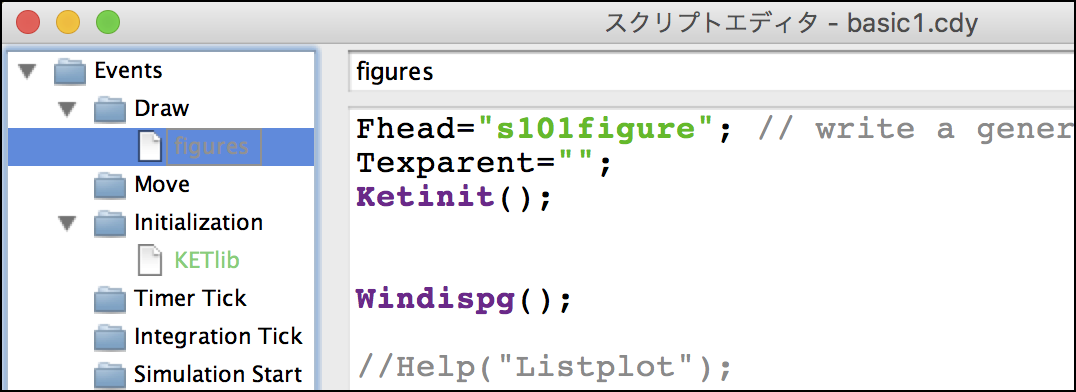
\includegraphics[bb=0 0 1076 392 , width=10cm]{Fig/slot.png}\\
 \\
 1つのスロットに複数のページを作ることができる。KETlib以外に初期設定のスクリプトを書く場合は,Initialzation スロットに新しいページを作るのがよい。\\


\subsection{プロットデータ} 
プロットデータ(Plot Data) とは,関数のグラフや幾何要素を描くデータのことであり,KeTCindyの処理の中核をなしている。本マニュアルでは PD と略すことがある。たとえば曲線は,描画範囲を分割して線分の集まりとして描画しており,このときのプロットデータはそれらの線分の端点のリストである。\\
 プロットデータの名称はKeTCindyが自動的に命名する。その命名規則は次の通りである。\\
\\
・名称の頭部は,プロットデータを作成する関数ごとに決まっている。\\
・第1引数に name が与えられる場合,name を頭部に付加する。\\
   例:\verb|Listplot("1",[[0,0],[1,2]]);| のとき,sg1\\
・関数によっては,第1引数の name を略すことができる。この場合,引数で用いられた点の名前を頭部に付加する。\\
   例:\verb|Listplot([A,B,C]);|    のとき,sgABC\\
 \\
 プロットデータを生成したときは,Cindyscriptエディタのコンソールにその名称を表示する。上の例では,\\
    \verb|generate Listplot sgABC|\\
と表示される。プロットデータを操作する関数では,このPDの名称を用いる。\\
 プロットデータの内容を知りたい場合は,Cindyscriptの\\
    println(プロットデータ名)\\
でコンソールに表示することができる。\\
 プロットデータは,Cindyscriptによるプログラムで作成してそれをKeTCindyで利用することもできる。Listplot()の例を参照のこと。ただし,要素の数が大きいとScilabでエラーとなるので,1つのプロットデータの要素は200程度とするのがよい。これより多い場合は分割する。\\

\subsection{Cinderellaの作図ツール}
  \\
\includegraphics[bb=0 0 27 21 , width=0.6cm]{Cindytool/move.png}  動かすモード(選択モード)にする:標準状態\\
\includegraphics[bb=0 0 27 21 , width=0.6cm]{Cindytool/single-add.png}  点を加える\\
\includegraphics[bb=0 0 27 21 , width=0.6cm]{Cindytool/multi-add-line.png}  直線を加える\\
\includegraphics[bb=0 0 27 21 , width=0.6cm]{Cindytool/segment.png}  線分を加える\\
\includegraphics[bb=0 0 27 21 , width=0.6cm]{Cindytool/middle.png}  中点を加える\\
\includegraphics[bb=0 0 27 21 , width=0.6cm]{Cindytool/intersection.png}  交点を加える\\
\includegraphics[bb=0 0 27 21 , width=0.6cm]{Cindytool/multi-add-parallel.png}  平行線を加える\\
\includegraphics[bb=0 0 27 21 , width=0.6cm]{Cindytool/multi-add-perp.png}  垂線を加える\\
\includegraphics[bb=0 0 27 21 , width=0.6cm]{Cindytool/bisector.png}  角の二等分線を加える\\
\includegraphics[bb=0 0 27 21 , width=0.6cm]{Cindytool/multi-add-circle.png}  円を加える\\
\includegraphics[bb=0 0 27 21 , width=0.6cm]{Cindytool/circle-by-radius.png}  半径つき円を加える\\
\includegraphics[bb=0 0 27 21 , width=0.6cm]{Cindytool/ellipse-by-foci.png}  焦点と通る点で決まる楕円\\
\includegraphics[bb=0 0 27 21 , width=0.6cm]{Cindytool/hyperbola-by-foci.png}  焦点と通る点で決まる双曲線\\
\includegraphics[bb=0 0 27 21 , width=0.6cm]{Cindytool/parabola-by-foci.png}  焦点と準線で決まる放物線\\
\includegraphics[bb=0 0 27 21 , width=0.6cm]{Cindytool/polygon.png}  多角形を加える\\
\includegraphics[bb=0 0 27 21 , width=0.6cm]{Cindytool/angle-mark.png}  角に印をつける\\
\includegraphics[bb=0 0 27 21 , width=0.6cm]{Cindytool/angle.png}  角度を測る\\
\includegraphics[bb=0 0 27 21 , width=0.6cm]{Cindytool/delete.png}  選択した要素を消去する\\
\includegraphics[bb=0 0 27 21 , width=0.6cm]{Cindytool/select-points.png}  点をまとめて選択する\\
\includegraphics[bb=0 0 27 21 , width=0.6cm]{Cindytool/select-lines.png}  線分をまとめて選択する\\
 \\
設定メニューから「上のツールバーのカスタマイズ」を選び,「すべて表示」にすると現れるツール\\
\includegraphics[bb=0 0 27 21 , width=0.6cm]{Cindytool/mirror.png}  鏡映\\
\includegraphics[bb=0 0 27 21 , width=0.6cm]{Cindytool/polar-of-point.png}  点の極線を描く\\
 \\
画面ツール(下のツールバー)\\
\includegraphics[bb=0 0 27 21 , width=0.6cm]{Cindytool/translate-view.png}  原点を移動する\\
\includegraphics[bb=0 0 27 21 , width=0.6cm]{Cindytool/zoom-in.png}  矩形領域を画面サイズに拡大\\
\includegraphics[bb=0 0 27 21 , width=0.6cm]{Cindytool/zoom-out.png}  画面を矩形領域サイズに縮小\\
\includegraphics[bb=0 0 27 21 , width=0.6cm]{Cindytool/snap.png}  軸と方眼を表示し格子点にスナップする\\

\subsection{用語解説} 
インシデント\\ 
 点が曲線上に乗っている状態を表す。\\
インスペクタ\\
 幾何要素の属性などを管理するウィンドウ。\\
幾何要素  \\
 Cinderellaの作図ツールで作図した点や直線などの要素\\
幾何点 \\
 幾何要素としての点。マウスドラッグで動かすことができる。\\
固定点\\
 マウスドラッグで移動することのできない点\\
コンソール\\
 スクリプトエディタの右下のエリア。\\
自由点\\
 マウスドラッグで任意に動かすことのできる点。\\
スロット  \\
 Cindyscriptで,スクリプトを書くとき,実行タイミングによりに分類するもの\\ 
スナップ \\
 マウスポイントが格子点の近くに来ると格子点上にぴったり移動する。\\
 Cinderellaの画面の下方ツールのうち,磁石アイコンによりこのモードになる。\\

\newpage
%=======================
\section{定数と変数}
KeTCindy は Cindyscript で記述されている。CindyScriptでは,変数名は大文字と小文字を区別するが,関数名は大文字小文字を区別しない。Cindyscriptのマニュアルでは組み込み関数名はすべて小文字で表記されている。例示されたスクリプトでは,変数も小文字である。そこで,KeTCindyでは,組み込みの変数名・関数名と区別しやすいように,次の規則により名前を付けている。\\
 \\
 ・グローバルな変数はすべて大文字か,大文字で始まるものとする。\\
 ・局所変数は小文字で,関数定義の冒頭で regional() により局所変数として宣言する。\\
 ・関数名は大文字で始まる。\\
 \\
 なお,CindyScriptは関数型プログラミング言語であり,命令はすべて関数を用いて行われるが,本マニュアルでは,文脈により「コマンド」という表現も用いる。\\
 \\
{\bf 定数} \\
 つぎのものがCindyScriptに予約されており,小文字で表されている。\\

\begin{tabbing}
12345678\=\kill
  pi   \>:円周率。Scilabには \% pi で書き出される。\\
  i  \> :虚数単位。Scilabには \% i で書き出される。\\
\end{tabbing}
 一般のプログラミングでは変数 i をループ変数としてよく使うが,CindyScript では i は予約定数と考え,変数として用いないことを勧める。ただし,変数としてまったく使えないわけではなく,変数として用いた後,必要があれば \verb|i=complex([0,1])|  を実行することにより虚数単位として再定義することができる。\\
 \\
{\bf 予約変数}\\
 KeTCindy が内部的に使用する予約変数がある。そのうち次のものはユーザーが値を変更または設定することができる。設定は Initalization スロットの「KETlib」ページでおこなうが,Fhead とTexparent は Draw スロットでもよい。\\
\begin{tabbing}
1234567890123\=45678989012345678901234567890123\=\kill
 Fhead \>書き出されるファイル名の頭部\\
 Texparent \>親プロセスのファイル名\\
 Dirhead \>パスの頭部\\
 Dirlib \>ライブラリ ketlib のパス\\
 Dirbin \>ketbin のパス\\
 Dirwork \>作業ディレクトリのパス\\
 Shellfile \>シェルファイル名\\
\end{tabbing}
 以下の予約変数は,ライブラリが使用するグローバル変数であるので,ユーザーはこれらの変数名を使ってはいけない。なお,変数は大文字小文字を区別するので,小文字で書く分には支障はない。したがって,ユーザーが作るプログラムでは,すべて小文字か,先頭だけが大文字の変数を使うことを勧める。\\
 \\
ADDAXES, ArrowlineNumber, ArrowheadNumber, BezierNumber,\\
COM0thlist, COM1stlist, COM2ndlist, Dq, FUNLIST,\\
Fnamesc ,Fnamescibody,Fnameout,Fnametex,GDATALIST,\\
GLIST, GCLIST, GOUTLIST, KCOLOR, KETPICCOUNT, \\
KETPICLAYER, LETTERlist, LFmark, MilliIn, PenThick, \\
PenThickInit, POUTLIST, SCALEX, SCALEY, SCIRELIST, \\
SCIWRLIST, TenSize, TenSizeInit, ULEN, XMAX, XMIN, YaSize,\\
YaThick, YMAX, YMIN, VLIST

\newpage

%設定・定義 ==================================
\section{関数リファレンス}
\subsection{設定・定義}

\begin{description}

\hypertarget{addax}{}
\item[関数] Addax(0または1)
\item[機能] 座標軸を書くかどうかを定める
\item[説明] ScilabのClosefile() の引数に対応する。\\
 引数が0のとき座標軸を書かない(デフォルトは1)
\begin{verbatim}
 Listplot([B,A,C]);
 Letter([A,"ne","A",B,"se","B",C,"se","C"]);
\end{verbatim}
 \\
 %%% test.tex 2014-10-16 21:49
%%% test.sce 2014-10-16 21:49
{\unitlength=1cm%
\begin{picture}%
(   4.00000,   3.50000)(  -1.00000,  -1.00000)%
\special{pn 8}%
%
\settowidth{\Width}{A}\setlength{\Width}{0\Width}%
\settoheight{\Height}{A}\settodepth{\Depth}{A}\setlength{\Height}{\Depth}%
\put(1.0300,1.7900){\hspace*{\Width}\raisebox{\Height}{A}}%
%
%
\settowidth{\Width}{B}\setlength{\Width}{0\Width}%
\settoheight{\Height}{B}\settodepth{\Depth}{B}\setlength{\Height}{-\Height}%
\put(0.0500,-0.0500){\hspace*{\Width}\raisebox{\Height}{B}}%
%
%
\settowidth{\Width}{C}\setlength{\Width}{0\Width}%
\settoheight{\Height}{C}\settodepth{\Depth}{C}\setlength{\Height}{-\Height}%
\put(2.0500,-0.0500){\hspace*{\Width}\raisebox{\Height}{C}}%
%
%
\special{pa 0 0}\special{pa 386 -685}\special{pa 787 0}%
\special{fp}%
\special{pa -394 0}\special{pa 1181 0}%
\special{fp}%
\special{pa 0 394}\special{pa 0 -984}%
\special{fp}%
\settowidth{\Width}{$x$}\setlength{\Width}{0\Width}%
\settoheight{\Height}{$x$}\settodepth{\Depth}{$x$}\setlength{\Height}{-0.5\Height}\setlength{\Depth}{0.5\Depth}\addtolength{\Height}{\Depth}%
\put(3.0500,0.0000){\hspace*{\Width}\raisebox{\Height}{$x$}}%
%
%
\settowidth{\Width}{$y$}\setlength{\Width}{-0.5\Width}%
\settoheight{\Height}{$y$}\settodepth{\Depth}{$y$}\setlength{\Height}{\Depth}%
\put(0.0000,2.5500){\hspace*{\Width}\raisebox{\Height}{$y$}}%
%
%
\settowidth{\Width}{O}\setlength{\Width}{-1\Width}%
\settoheight{\Height}{O}\settodepth{\Depth}{O}\setlength{\Height}{-\Height}%
\put(-0.0500,-0.0500){\hspace*{\Width}\raisebox{\Height}{O}}%
%
%
\end{picture}}%
\begin{verbatim}
 Listplot([B,A,C,B]);
 Letter([A,"ne","A",B,"sw","B",C,"se","C"]);
 Addax(0);
\end{verbatim}
 %%% test.tex 2014-10-16 21:51
%%% test.sce 2014-10-16 21:50
{\unitlength=1cm%
\begin{picture}%
(   4.00000,   3.50000)(  -1.00000,  -1.00000)%
\special{pn 8}%
%
\settowidth{\Width}{A}\setlength{\Width}{0\Width}%
\settoheight{\Height}{A}\settodepth{\Depth}{A}\setlength{\Height}{\Depth}%
\put(1.0300,1.7900){\hspace*{\Width}\raisebox{\Height}{A}}%
%
%
\settowidth{\Width}{B}\setlength{\Width}{-1\Width}%
\settoheight{\Height}{B}\settodepth{\Depth}{B}\setlength{\Height}{-\Height}%
\put(-0.0500,-0.0500){\hspace*{\Width}\raisebox{\Height}{B}}%
%
%
\settowidth{\Width}{C}\setlength{\Width}{0\Width}%
\settoheight{\Height}{C}\settodepth{\Depth}{C}\setlength{\Height}{-\Height}%
\put(2.0500,-0.0500){\hspace*{\Width}\raisebox{\Height}{C}}%
%
%
\special{pa 0 0}\special{pa 386 -685}\special{pa 787 0}\special{pa 0 0}%
\special{fp}%
\end{picture}}%\\
\begin{flushright} \hyperlink{functionlist}{$\Rightarrow$関数一覧}\end{flushright}
 \\
\hypertarget{addcolor}{}
\item[関数] Addcolor(描画コマンド , カラーコード)
\item[機能] 描画コマンドで描かれる線を指定色で描く
\item[説明] 描画コマンドはダブルクウォートでくくって文字列とする。描画コマンド内にダブルクウォートがある場合は,シングルクウォートにする。optionのある描画コマンドでoptionを指定しない場合は,必ず空リストをoptionとして書く。描画色は,RGBまたはCMYK。描画色は画面と図版の両方に有効。\\
 \\
 例:\verb|Addcolor("Plotdata('2','x^2','x',[])",[1,1,0]);|\\
 \\
 \\
\hypertarget{colorcode}{}
\item[関数] Colorcode(文字1,文字2, カラーコード)
\item[機能] 文字1から文字2へカラーコードを変換する。戻り値は変換されたコード。
\item[説明] 文字は,"rgb","cmyk","hsv"のいずれか。\\
 \\
例:\verb|Colorcode("rgb","cmyk",[1,0,0]); |\\
     RGBコードの[1,0,0]をCMYKに変換したコードを返す\\
  \verb|Colorcode("cmyk","rgb",[0,1,1,0]);|\\
    CMYKコードの[0,1,1,0]をRGBに変換したコードを返す\\
  \verb|Colorcode("rgb","hsv",[1,0,0]);|\\
    RGBコードの[1,0,0]をHSVに変換したコードを返す\\
 \\
 \\
\hypertarget{deffun}{}
\item[関数] Deffun(関数名 , 定義のリスト)
\item[機能] 関数を定義する
\item[説明] 関数定義は,CindyScript の関数定義 f(x):=式 でもできるが,Deffun()を使うことにより,Scilab 側に渡すファイルに\\
 function 定義式 endfunction;\\
 が記述されるので,Scilab側でこの関数を利用することができる。目的に応じて使い分けるとよい。\\
 式のリストには if文を用いた場合分けの関数式を記述することもできる。\\
 \\
例:$f(x)=\dfrac{1}{x^2+1}$ を定義し,グラフを描いてx=1 における微分係数を求める。
\begin{verbatim}
   Deffun("f(x)",["regional(y)","y=1/(x\verb|^|2+1)","y"]);
   Plotdata("1","f(x)","x");
   coeff=Derivative("f(x)","x",1);
\end{verbatim}
  点Aを作図しておくと,点Aをドラッグしたとき常に曲線上に乗せ,その点での\\
  接線を引くことができる。
\begin{verbatim}
   A.xy=[A.x,f(A.x)];
   coeff=Derivative("f(x)","x",A.x);
   Lineplot("1",[A,[A.x+1,A.y+coeff]]);
\end{verbatim}
     %%% test.tex 2014-10-16 22:5
%%% test.sce 2014-10-16 22:5
{\unitlength=1cm%
\begin{picture}%
(   6.00000,   3.00000)(  -3.00000,  -1.00000)%
\special{pn 8}%
%
\settowidth{\Width}{A}\setlength{\Width}{0\Width}%
\settoheight{\Height}{A}\settodepth{\Depth}{A}\setlength{\Height}{\Depth}%
\put(1.4400,0.3900){\hspace*{\Width}\raisebox{\Height}{A}}%
%
%
\special{pa -1181 -39}\special{pa -1133 -42}\special{pa -1085 -46}\special{pa -1036 -50}%
\special{pa -988 -54}\special{pa -940 -59}\special{pa -892 -64}\special{pa -844 -70}%
\special{pa -795 -77}\special{pa -747 -86}\special{pa -699 -95}\special{pa -651 -105}%
\special{pa -603 -118}\special{pa -554 -132}\special{pa -506 -148}\special{pa -458 -167}%
\special{pa -410 -189}\special{pa -362 -214}\special{pa -313 -241}\special{pa -265 -271}%
\special{pa -217 -302}\special{pa -169 -333}\special{pa -121 -360}\special{pa -72 -381}%
\special{pa -24 -392}\special{pa 24 -392}\special{pa 72 -381}\special{pa 121 -360}%
\special{pa 169 -333}\special{pa 217 -302}\special{pa 265 -271}\special{pa 313 -241}%
\special{pa 362 -214}\special{pa 410 -189}\special{pa 458 -167}\special{pa 506 -148}%
\special{pa 554 -132}\special{pa 603 -118}\special{pa 651 -105}\special{pa 699 -95}%
\special{pa 747 -86}\special{pa 795 -77}\special{pa 844 -70}\special{pa 892 -64}\special{pa 940 -59}%
\special{pa 988 -54}\special{pa 1036 -50}\special{pa 1085 -46}\special{pa 1133 -42}%
\special{pa 1181 -39}%
\special{fp}%
\special{pa -1181 -687}\special{pa 1181 69}%
\special{fp}%
\special{pa -1181 0}\special{pa 1181 0}%
\special{fp}%
\special{pa 0 394}\special{pa 0 -787}%
\special{fp}%
\settowidth{\Width}{$x$}\setlength{\Width}{0\Width}%
\settoheight{\Height}{$x$}\settodepth{\Depth}{$x$}\setlength{\Height}{-0.5\Height}\setlength{\Depth}{0.5\Depth}\addtolength{\Height}{\Depth}%
\put(3.0500,0.0000){\hspace*{\Width}\raisebox{\Height}{$x$}}%
%
%
\settowidth{\Width}{$y$}\setlength{\Width}{-0.5\Width}%
\settoheight{\Height}{$y$}\settodepth{\Depth}{$y$}\setlength{\Height}{\Depth}%
\put(0.0000,2.0500){\hspace*{\Width}\raisebox{\Height}{$y$}}%
%
%
\settowidth{\Width}{O}\setlength{\Width}{-1\Width}%
\settoheight{\Height}{O}\settodepth{\Depth}{O}\setlength{\Height}{-\Height}%
\put(-0.0500,-0.0500){\hspace*{\Width}\raisebox{\Height}{O}}%
%
%
\end{picture}}%\\

 例:$f(x)=\left\{\begin{array}{l}1  (x\geqq 0)\\ -1  (x<0)\\ \end{array}\right.$   を定義する。
\begin{verbatim}
  Deffun("f(x)",["regional(y)","if(x>=0,y=1,y=-1)","y"]);
\end{verbatim}
 if 文はネストすることができる。
\begin{verbatim}
  Deffun("f(x)",["regional y","if(x>1,y=1,
        if(x>-1,y=x,y=-1))","y"]);
\end{verbatim}
 \\


\hypertarget{defvar}{}
\item[関数] Defvar(文字列)
\item[機能] 変数を定義する
\item[説明] 変数の定義をScilabと共有する。また,ScilabのAssignリストに追加する。\\
 \\
   例:\verb|Defvar("const=3");|
 \\
\hypertarget{drwxy}{}
\item[関数] Drwxy()
\item[機能] 座標軸を描く
\item[説明] 座標軸はデフォルトでは最後に描かれるが,座標軸上に白抜きの点を表示するなど,先に描くことが必要な場合に用いる。\\

例:点$(-\pi,\ 0)$と$(\pi,\ 0)$を白抜きの点で表示する。
\begin{verbatim}
  Setax([7,"se"]);
  Setpt(8);
  Drwpt([-pi,0],0);
  Drwxy();
  Plotdata("1","sin(x)","x",["dr","Num=300"]);
  Drwpt([[pi,0],0]);
\end{verbatim}

 このスクリプトでは,Drwpt([-pi,0],0); を実行したのち座標軸を描き,次に,$y=\sin x$ のグラフを描いてから Drwpt([pi,0],0);を実行するので,点($-\pi$,0) の上を座標軸が通り,点($\pi$,0)は座標軸とグラフの上を通るので白抜きになる。\\

%%% drwxy.tex 2014-11-7 18:44
%%% drwxy.sce 2014-11-7 17:31
{\unitlength=1cm%
\begin{picture}%
(  12.00000,   4.00000)(  -6.00000,  -2.00000)%
\special{pn 8}%
%
\special{pa -1215 -22}\special{pa -1224 -29}\special{pa -1235 -31}\special{pa -1247 -30}%
\special{pa -1257 -24}\special{pa -1264 -15}\special{pa -1268 -4}\special{pa -1268 7}%
\special{pa -1263 18}\special{pa -1255 26}\special{pa -1244 31}\special{pa -1232 31}%
\special{pa -1222 28}\special{pa -1213 20}\special{pa -1207 10}\special{pa -1205 -1}%
\special{pa -1208 -13}\special{pa -1215 -22}\special{sh 0}\special{fp}%
\special{pa -2362 0}\special{pa 2362 0}%
\special{fp}%
\special{pa 0 787}\special{pa 0 -787}%
\special{fp}%
\settowidth{\Width}{$x$}\setlength{\Width}{0\Width}%
\settoheight{\Height}{$x$}\settodepth{\Depth}{$x$}\setlength{\Height}{-0.5\Height}\setlength{\Depth}{0.5\Depth}\addtolength{\Height}{\Depth}%
\put(6.0500,0.0000){\hspace*{\Width}\raisebox{\Height}{$x$}}%
%
%
\settowidth{\Width}{$y$}\setlength{\Width}{-0.5\Width}%
\settoheight{\Height}{$y$}\settodepth{\Depth}{$y$}\setlength{\Height}{\Depth}%
\put(0.0000,2.0500){\hspace*{\Width}\raisebox{\Height}{$y$}}%
%
%
\settowidth{\Width}{O}\setlength{\Width}{0\Width}%
\settoheight{\Height}{O}\settodepth{\Depth}{O}\setlength{\Height}{-\Height}%
\put(0.0500,-0.0500){\hspace*{\Width}\raisebox{\Height}{O}}%
%
%
\special{pa -2362 -110}\special{pa -2346 -125}\special{pa -2331 -140}\special{pa -2315 -155}%
\special{pa -2299 -169}\special{pa -2283 -183}\special{pa -2267 -197}\special{pa -2252 -211}%
\special{pa -2236 -224}\special{pa -2220 -237}\special{pa -2204 -249}\special{pa -2188 -261}%
\special{pa -2173 -273}\special{pa -2157 -284}\special{pa -2141 -294}\special{pa -2125 -305}%
\special{pa -2109 -314}\special{pa -2094 -324}\special{pa -2078 -332}\special{pa -2062 -341}%
\special{pa -2046 -348}\special{pa -2030 -355}\special{pa -2015 -362}\special{pa -1999 -368}%
\special{pa -1983 -373}\special{pa -1967 -378}\special{pa -1951 -382}\special{pa -1936 -386}%
\special{pa -1920 -388}\special{pa -1904 -391}\special{pa -1888 -392}\special{pa -1872 -393}%
\special{pa -1857 -394}\special{pa -1841 -393}\special{pa -1825 -393}\special{pa -1809 -391}%
\special{pa -1793 -389}\special{pa -1778 -386}\special{pa -1762 -383}\special{pa -1746 -379}%
\special{pa -1730 -374}\special{pa -1714 -369}\special{pa -1699 -363}\special{pa -1683 -357}%
\special{pa -1667 -350}\special{pa -1651 -342}\special{pa -1635 -334}\special{pa -1620 -325}%
\special{pa -1604 -316}\special{pa -1588 -306}\special{pa -1572 -296}\special{pa -1556 -286}%
\special{pa -1541 -274}\special{pa -1525 -263}\special{pa -1509 -251}\special{pa -1493 -239}%
\special{pa -1477 -226}\special{pa -1462 -213}\special{pa -1446 -199}\special{pa -1430 -185}%
\special{pa -1414 -171}\special{pa -1398 -157}\special{pa -1383 -142}\special{pa -1367 -128}%
\special{pa -1351 -113}\special{pa -1335 -97}\special{pa -1319 -82}\special{pa -1304 -66}%
\special{pa -1288 -51}\special{pa -1272 -35}\special{pa -1256 -19}\special{pa -1240 -4}%
\special{pa -1225 12}\special{pa -1209 28}\special{pa -1193 44}\special{pa -1177 59}%
\special{pa -1161 75}\special{pa -1146 90}\special{pa -1130 106}\special{pa -1114 121}%
\special{pa -1098 136}\special{pa -1082 151}\special{pa -1067 165}\special{pa -1051 179}%
\special{pa -1035 193}\special{pa -1019 207}\special{pa -1003 220}\special{pa -988 233}%
\special{pa -972 246}\special{pa -956 258}\special{pa -940 269}\special{pa -924 281}%
\special{pa -909 292}\special{pa -893 302}\special{pa -877 312}\special{pa -861 321}%
\special{pa -845 330}\special{pa -830 338}\special{pa -814 346}\special{pa -798 353}%
\special{pa -782 360}\special{pa -766 366}\special{pa -751 372}\special{pa -735 377}%
\special{pa -719 381}\special{pa -703 385}\special{pa -687 388}\special{pa -672 390}%
\special{pa -656 392}\special{pa -640 393}\special{pa -624 394}\special{pa -608 394}%
\special{pa -593 393}\special{pa -577 391}\special{pa -561 390}\special{pa -545 387}%
\special{pa -529 384}\special{pa -514 380}\special{pa -498 375}\special{pa -482 370}%
\special{pa -466 365}\special{pa -450 358}\special{pa -435 352}\special{pa -419 344}%
\special{pa -403 336}\special{pa -387 328}\special{pa -371 319}\special{pa -356 309}%
\special{pa -340 299}\special{pa -324 289}\special{pa -308 278}\special{pa -292 266}%
\special{pa -277 254}\special{pa -261 242}\special{pa -245 229}\special{pa -229 216}%
\special{pa -213 203}\special{pa -198 189}\special{pa -182 175}\special{pa -166 161}%
\special{pa -150 146}\special{pa -134 132}\special{pa -119 117}\special{pa -103 102}%
\special{pa -87 86}\special{pa -71 71}\special{pa -55 55}\special{pa -40 39}\special{pa -24 24}%
\special{pa -8 8}\special{pa 8 -8}\special{pa 24 -24}\special{pa 40 -39}\special{pa 55 -55}%
\special{pa 71 -71}\special{pa 87 -86}\special{pa 103 -102}\special{pa 119 -117}\special{pa 134 -132}%
\special{pa 150 -146}\special{pa 166 -161}\special{pa 182 -175}\special{pa 198 -189}%
\special{pa 213 -203}\special{pa 229 -216}\special{pa 245 -229}\special{pa 261 -242}%
\special{pa 277 -254}\special{pa 292 -266}\special{pa 308 -278}\special{pa 324 -289}%
\special{pa 340 -299}\special{pa 356 -309}\special{pa 371 -319}\special{pa 387 -328}%
\special{pa 403 -336}\special{pa 419 -344}\special{pa 435 -352}\special{pa 450 -358}%
\special{pa 466 -365}\special{pa 482 -370}\special{pa 498 -375}\special{pa 514 -380}%
\special{pa 529 -384}\special{pa 545 -387}\special{pa 561 -390}\special{pa 577 -391}%
\special{pa 593 -393}\special{pa 608 -394}\special{pa 624 -394}\special{pa 640 -393}%
\special{pa 656 -392}\special{pa 672 -390}\special{pa 687 -388}\special{pa 703 -385}%
\special{pa 719 -381}\special{pa 735 -377}\special{pa 751 -372}\special{pa 766 -366}%
\special{pa 782 -360}\special{pa 798 -353}\special{pa 814 -346}\special{pa 830 -338}%
\special{pa 845 -330}\special{pa 861 -321}\special{pa 877 -312}\special{pa 893 -302}%
\special{pa 909 -292}\special{pa 924 -281}\special{pa 940 -269}\special{pa 956 -258}%
\special{pa 972 -246}\special{pa 988 -233}\special{pa 1003 -220}\special{pa 1019 -207}%
\special{pa 1035 -193}\special{pa 1051 -179}\special{pa 1067 -165}\special{pa 1082 -151}%
\special{pa 1098 -136}\special{pa 1114 -121}\special{pa 1130 -106}\special{pa 1146 -90}%
\special{pa 1161 -75}\special{pa 1177 -59}\special{pa 1193 -44}\special{pa 1209 -28}%
\special{pa 1225 -12}\special{pa 1240 4}\special{pa 1256 19}\special{pa 1272 35}\special{pa 1288 51}%
\special{pa 1304 66}\special{pa 1319 82}\special{pa 1335 97}\special{pa 1351 113}%
\special{pa 1367 128}\special{pa 1383 142}\special{pa 1398 157}\special{pa 1414 171}%
\special{pa 1430 185}\special{pa 1446 199}\special{pa 1462 213}\special{pa 1477 226}%
\special{pa 1493 239}\special{pa 1509 251}\special{pa 1525 263}\special{pa 1541 274}%
\special{pa 1556 286}\special{pa 1572 296}\special{pa 1588 306}\special{pa 1604 316}%
\special{pa 1620 325}\special{pa 1635 334}\special{pa 1651 342}\special{pa 1667 350}%
\special{pa 1683 357}\special{pa 1699 363}\special{pa 1714 369}\special{pa 1730 374}%
\special{pa 1746 379}\special{pa 1762 383}\special{pa 1778 386}\special{pa 1793 389}%
\special{pa 1809 391}\special{pa 1825 393}\special{pa 1841 393}\special{pa 1857 394}%
\special{pa 1872 393}\special{pa 1888 392}\special{pa 1904 391}\special{pa 1920 388}%
\special{pa 1936 386}\special{pa 1951 382}\special{pa 1967 378}\special{pa 1983 373}%
\special{pa 1999 368}\special{pa 2015 362}\special{pa 2030 355}\special{pa 2046 348}%
\special{pa 2062 341}\special{pa 2078 332}\special{pa 2094 324}\special{pa 2109 314}%
\special{pa 2125 305}\special{pa 2141 294}\special{pa 2157 284}\special{pa 2173 273}%
\special{pa 2188 261}\special{pa 2204 249}\special{pa 2220 237}\special{pa 2236 224}%
\special{pa 2252 211}\special{pa 2267 197}\special{pa 2283 183}\special{pa 2299 169}%
\special{pa 2315 155}\special{pa 2331 140}\special{pa 2346 125}\special{pa 2362 110}%
\special{fp}%
\special{pa 1259 -22}\special{pa 1250 -29}\special{pa 1238 -31}\special{pa 1227 -30}%
\special{pa 1217 -24}\special{pa 1209 -15}\special{pa 1206 -4}\special{pa 1206 7}%
\special{pa 1211 18}\special{pa 1219 26}\special{pa 1230 31}\special{pa 1241 31}\special{pa 1252 28}%
\special{pa 1261 20}\special{pa 1267 10}\special{pa 1268 -1}\special{pa 1266 -13}%
\special{pa 1259 -22}\special{sh 0}\special{fp}%
\end{picture}}%
 \\
 \\
\hypertarget{fontsize}{}
\item[関数] Fontsize(記号)
\item[機能] フォントサイズを設定する
\item[説明] 次に Fontsize() を実行するまで有効\\
 記号は,"t" , "ss" , "f", "s" , "n" , "la",  "La", "LA", "h" , "H"\\

例:小さい方からいくつか表示する。
\begin{verbatim}
  Ptsize(2);
  Drawpoint([A,B,C,D,E,F,G]);
  Fontsize("t"); Letter([A,"s2","A"]);
  Fontsize("ss"); Letter([B,"s2","B"]);
  Fontsize("s"); Letter([C,"s2","C"]);
  Fontsize("la"); 	Letter([D,"s2","D"]);
  Fontsize("La"); Letter([E,"s2","E"]);
  Fontsize("h"); Letter([F,"s2","F"]);
  Fontsize("H"); Letter([G,"s2","G"]);
\end{verbatim}
  %%% test.tex 2014-11-28 20:51
%%% test.sce 2014-11-28 20:51
{\unitlength=6mm%
\begin{picture}%
(  14.00000,   2.00000)(  -1.00000,   2.00000)%
\special{pn 8}%
%
\special{pa 6 -714}\special{pa 0 -717}\special{pa -6 -714}\special{pa -8 -709}\special{pa -6 -703}%
\special{pa 0 -701}\special{pa 6 -703}\special{pa 8 -709}\special{pa 6 -714}\special{sh 1}\special{fp}%
\special{pa 478 -714}\special{pa 472 -717}\special{pa 467 -714}\special{pa 465 -709}%
\special{pa 467 -703}\special{pa 472 -701}\special{pa 478 -703}\special{pa 480 -709}%
\special{pa 478 -714}\special{sh 1}\special{fp}%
\special{pa 950 -714}\special{pa 945 -717}\special{pa 939 -714}\special{pa 937 -709}%
\special{pa 939 -703}\special{pa 945 -701}\special{pa 950 -703}\special{pa 953 -709}%
\special{pa 950 -714}\special{sh 1}\special{fp}%
\special{pa 1423 -714}\special{pa 1417 -717}\special{pa 1412 -714}\special{pa 1409 -709}%
\special{pa 1412 -703}\special{pa 1417 -701}\special{pa 1423 -703}\special{pa 1425 -709}%
\special{pa 1423 -714}\special{sh 1}\special{fp}%
\special{pa 1895 -714}\special{pa 1890 -717}\special{pa 1884 -714}\special{pa 1882 -709}%
\special{pa 1884 -703}\special{pa 1890 -701}\special{pa 1895 -703}\special{pa 1898 -709}%
\special{pa 1895 -714}\special{sh 1}\special{fp}%
\special{pa 2368 -714}\special{pa 2362 -717}\special{pa 2357 -714}\special{pa 2354 -709}%
\special{pa 2357 -703}\special{pa 2362 -701}\special{pa 2368 -703}\special{pa 2370 -709}%
\special{pa 2368 -714}\special{sh 1}\special{fp}%
\special{pa 2840 -714}\special{pa 2835 -717}\special{pa 2829 -714}\special{pa 2827 -709}%
\special{pa 2829 -703}\special{pa 2835 -701}\special{pa 2840 -703}\special{pa 2843 -709}%
\special{pa 2840 -714}\special{sh 1}\special{fp}%
\tiny%
\settowidth{\Width}{A}\setlength{\Width}{-0.5\Width}%
\settoheight{\Height}{A}\settodepth{\Depth}{A}\setlength{\Height}{-\Height}%
\put(0.0000,2.8500){\hspace*{\Width}\raisebox{\Height}{A}}%
%
%
\scriptsize%
\settowidth{\Width}{B}\setlength{\Width}{-0.5\Width}%
\settoheight{\Height}{B}\settodepth{\Depth}{B}\setlength{\Height}{-\Height}%
\put(2.0000,2.8500){\hspace*{\Width}\raisebox{\Height}{B}}%
%
%
\small%
\settowidth{\Width}{C}\setlength{\Width}{-0.5\Width}%
\settoheight{\Height}{C}\settodepth{\Depth}{C}\setlength{\Height}{-\Height}%
\put(4.0000,2.8500){\hspace*{\Width}\raisebox{\Height}{C}}%
%
%
\large%
\settowidth{\Width}{D}\setlength{\Width}{-0.5\Width}%
\settoheight{\Height}{D}\settodepth{\Depth}{D}\setlength{\Height}{-\Height}%
\put(6.0000,2.8500){\hspace*{\Width}\raisebox{\Height}{D}}%
%
%
\Large%
\settowidth{\Width}{E}\setlength{\Width}{-0.5\Width}%
\settoheight{\Height}{E}\settodepth{\Depth}{E}\setlength{\Height}{-\Height}%
\put(8.0000,2.8500){\hspace*{\Width}\raisebox{\Height}{E}}%
%
%
\huge%
\settowidth{\Width}{F}\setlength{\Width}{-0.5\Width}%
\settoheight{\Height}{F}\settodepth{\Depth}{F}\setlength{\Height}{-\Height}%
\put(10.0000,2.8500){\hspace*{\Width}\raisebox{\Height}{F}}%
%
%
\Huge%
\settowidth{\Width}{G}\setlength{\Width}{-0.5\Width}%
\settoheight{\Height}{G}\settodepth{\Depth}{G}\setlength{\Height}{-\Height}%
\put(12.0000,2.8500){\hspace*{\Width}\raisebox{\Height}{G}}%
%
%
\end{picture}}%

\begin{flushright} \hyperlink{functionlist}{$\Rightarrow$関数一覧}\end{flushright}
\newpage
\hypertarget{ketinit}{}
\item[関数] Ketinit(options)
\item[機能] \ketcindy を初期化する
\item[説明] opution 縦方向の倍率と描画領域を設定\\

 例:\verb|Ketinit()|   :倍率1,描画領域 $-5 \leqq x \leqq 5 , -5 \leqq y \leqq 5$(デフォルト)\\
   \verb|Ketinit(2)| : 倍率2,描画領域 $-5 \leqq x \leqq 5 , -5 \leqq y \leqq 5$\\
   \verb|Ketinit(2,[-2,3],[-2,4])| : 倍率2,描画領域 $-2 \leqq x \leqq 3 , -2 \leqq y \leqq 4$\\

 描画領域(TeXに出力する領域)は制御点SW(左下)とNE(右上)を対角とする矩形領域。描画領域を指定すると,制御点がなければその位置に作り,すでに存在する場合は何もしない。作成された制御点はドラッグして描画領域を変更することができる。\\
 倍率は,Setscaling(倍率)を実行するのと同じ。ただし,Cinderellaで作図した幾何要素に対しては無効。(Setscaling()の項参照)\\

\begin{flushright} \hyperlink{functionlist}{$\Rightarrow$関数一覧}\end{flushright}

\hypertarget{ptsie}{}
\item[関数] Ptsize(n) , Setpt(n)
\item[機能] 表示する点の大きさを設定する。
\item[説明] Ptsize() と Setpt() は同じである。デフォルトは1\\
 Ptsize()はCindyScript風の語法,Setpt() は \ketpic 風の語法\\
 全体の点の大きさを設定する。点の大きさを個々に変えたい場合は,sizeオプションを用いる。\\

例:1から4までの点の大きさ\\
 あらかじめ,Cinderellaの作図ツールで点A,B,C,Dを作図しておく。
\begin{verbatim}
  Pointdata("1",A,["size=1"]);
  Pointdata("2",B,["size=2"]);
  Pointdata("3",C,["size=3"]);
  Pointdata("4",D,["size=4"]);
\end{verbatim}

%%% test.tex 2014-10-22 9:7
%%% test.sce 2014-10-22 9:7
{\unitlength=1cm%
\begin{picture}%
(   7.00000,   2.00000)(  -3.00000,  -1.00000)%
\special{pn 8}%
%
\special{pa 3 -3}\special{pa -3 -3}\special{pa -3 3}\special{pa 3 3}\special{pa 3 -3}%
\special{sh 1}\special{fp}%
\special{pa 399 -6}\special{pa 394 -8}\special{pa 388 -6}\special{pa 386 0}\special{pa 388 6}%
\special{pa 394 8}\special{pa 399 6}\special{pa 402 0}\special{pa 399 -6}\special{sh 1}\special{fp}%
\special{pa 796 -8}\special{pa 789 -12}\special{pa 782 -11}\special{pa 777 -5}\special{pa 776 2}%
\special{pa 779 8}\special{pa 786 12}\special{pa 793 11}\special{pa 798 5}\special{pa 799 -2}%
\special{pa 796 -8}\special{sh 1}\special{fp}%
\special{pa 1192 -11}\special{pa 1185 -15}\special{pa 1177 -15}\special{pa 1170 -11}%
\special{pa 1166 -4}\special{pa 1166 4}\special{pa 1170 11}\special{pa 1177 15}\special{pa 1185 15}%
\special{pa 1192 11}\special{pa 1196 4}\special{pa 1196 -4}\special{pa 1192 -11}\special{sh 1}\special{fp}%
\settowidth{\Width}{Pointsize}\setlength{\Width}{-0.5\Width}%
\settoheight{\Height}{Pointsize}\settodepth{\Depth}{Pointsize}\setlength{\Height}{\Depth}%
\put(-1.4400,0.1500){\hspace*{\Width}\raisebox{\Height}{Pointsize}}%
%
%
\settowidth{\Width}{1}\setlength{\Width}{-0.5\Width}%
\settoheight{\Height}{1}\settodepth{\Depth}{1}\setlength{\Height}{\Depth}%
\put(0.0000,0.1500){\hspace*{\Width}\raisebox{\Height}{1}}%
%
%
\settowidth{\Width}{2}\setlength{\Width}{-0.5\Width}%
\settoheight{\Height}{2}\settodepth{\Depth}{2}\setlength{\Height}{\Depth}%
\put(1.0000,0.1500){\hspace*{\Width}\raisebox{\Height}{2}}%
%
%
\settowidth{\Width}{3}\setlength{\Width}{-0.5\Width}%
\settoheight{\Height}{3}\settodepth{\Depth}{3}\setlength{\Height}{\Depth}%
\put(2.0000,0.1500){\hspace*{\Width}\raisebox{\Height}{3}}%
%
%
\settowidth{\Width}{4}\setlength{\Width}{-0.5\Width}%
\settoheight{\Height}{4}\settodepth{\Depth}{4}\setlength{\Height}{\Depth}%
\put(3.0000,0.1500){\hspace*{\Width}\raisebox{\Height}{4}}%
%
%
\end{picture}}%\\

\begin{flushright} \hyperlink{functionlist}{$\Rightarrow$関数一覧}\end{flushright}
\newpage
\hypertarget{setax}{}
\item[関数] Setax()
\item[機能] 座標軸の書式を設定する。
\item[説明] Scilabのみで実行する。Cinderellaの描画面に反映されない。\\
引数は順番に\\
 1. 軸の形状(直線は "l" ,矢印は "a")デフォルトは直線\\
 2. 横軸名 デフォルトは $x$ \\
 3. 横軸名の位置\\
 4. 縦軸名 デフォルトは$y$\\
 5. 縦軸名の位置\\
 6. 原点名 デフォルトはO\\
 7. 原点名の位置\\
それぞれダブルクウォートでくくる。\\
7つの引数のうちn番目だけを指定する場合は,[n,"内容"]で指定できる。\\
また,後方はデフォルトなら省略できる。\\

  例:座標軸の先端を矢印にし,原点の北西にOを書く。\\
    \verb|Setax(["a","","","","","","nw"]);|\\

  例:原点の北西にOを書く。\\
    \verb|Setax([7,"nw"]);|\\

  例:先端を矢印にし,横軸をθ,縦軸を$x$にして矢じりの左側に書く。\\
    \verb|Setax(["a","θ","","x","w"]);|\\
 \\
     %%% test.tex 2014-11-11 15:44
%%% test.sce 2014-11-11 15:44
{\unitlength=6mm%
\begin{picture}%
(  10.00000,   5.00000)(  -5.00000,  -2.00000)%
\special{pn 8}%
%
\special{pn 8}%
\special{pa -1181 0}\special{pa 1181 0}%
\special{fp}%
\special{pn 8}%
\special{pa 1106 24}\special{pa 1181 0}\special{pa 1106 -24}\special{pa 1106 0}\special{pa 1106 24}%
\special{sh 1}\special{ip}%
\special{pn 8}%
\special{pa 1106 24}\special{pa 1181 0}\special{pa 1106 -24}\special{pa 1106 0}\special{pa 1106 24}%
\special{fp}%
\special{pn 8}%
\special{pn 8}%
\special{pa 0 472}\special{pa 0 -709}%
\special{fp}%
\special{pn 8}%
\special{pa 24 -634}\special{pa 0 -709}\special{pa -24 -634}\special{pa 0 -634}\special{pa 24 -634}%
\special{sh 1}\special{ip}%
\special{pn 8}%
\special{pa 24 -634}\special{pa 0 -709}\special{pa -24 -634}\special{pa 0 -634}\special{pa 24 -634}%
\special{fp}%
\special{pn 8}%
\settowidth{\Width}{$θ$}\setlength{\Width}{0\Width}%
\settoheight{\Height}{$θ$}\settodepth{\Depth}{$\theta$}\setlength{\Height}{-0.5\Height}\setlength{\Depth}{0.5\Depth}\addtolength{\Height}{\Depth}%
\put(5.0500,0.0000){\hspace*{\Width}\raisebox{\Height}{$\theta$}}%
%
%
\settowidth{\Width}{$x$}\setlength{\Width}{-1\Width}%
\settoheight{\Height}{$x$}\settodepth{\Depth}{$x$}\setlength{\Height}{-0.5\Height}\setlength{\Depth}{0.5\Depth}\addtolength{\Height}{\Depth}%
\put(-0.0500,3.0000){\hspace*{\Width}\raisebox{\Height}{$x$}}%
%
%
\settowidth{\Width}{O}\setlength{\Width}{-1\Width}%
\settoheight{\Height}{O}\settodepth{\Depth}{O}\setlength{\Height}{-\Height}%
\put(-0.0500,-0.0500){\hspace*{\Width}\raisebox{\Height}{O}}%
%
%
\end{picture}}%
 \\

\begin{flushright} \hyperlink{functionlist}{$\Rightarrow$関数一覧}\end{flushright}
\newpage
\hypertarget{definecolor}{}
\item[関数] Definecolor(色名 , 定義のリスト)
\item[機能] 色名を定義する
\item[説明] ユーザー命名の色名を定義する。定義リストは RGBまたはCMYKのリスト\\
 各色0〜1の範囲で指定する。定義した色名は,Setcolor(color,options) で使うことができる。なお,KeTCindyでは,68色を色名で使うことができる。次の Setcolor(color,options) 参照)\\
 \\
 例:暗い紫色を darkmaz の名称で定義して使う。
\begin{verbatim}
   Definecolor("darkmaz",[0.8,0,0.8]);
   Setcolor("darkmaz");
\end{verbatim}
\hypertarget{setcolor}{}
 \\
 \\
\item[関数] Setcolor(color,options)
\item[機能] 描画色の設定
\item[説明] 引数colorはカラーコードまたは色の名称。\\
 カラーコードはRGBまたはCMYKをリストで与える。各色0〜1。\\
 色の名称は次頁の68色が指定できる。ただし,Cinderellaの画面には色は反映されない。\\
 colorに色の名称を用いた場合は,option として,透明度を0〜1の数で指定できる。1が最も濃く,0は結果として色塗りをしない。\\
 \\
例 Cinderellaの描画ツールとCindyScriptで線分AB,ACを60°の角をなすように描いておき,点DとEを弧の両端になるように設定して
\begin{verbatim}
   Setcolor([1,0,0]);
   Circledata([A,D],["Rng=[0,pi/3]"]);
   Arrowhead(E,[-1,0.8],[2,1]);
\end{verbatim}
 を実行すると,矢じりつきの弧を赤で表示することができる。\\
 1行目は,\verb|Setcolor("red");| でもよい。\\
 ただし,Cinderellaの描画面では着色されない。\\
 描画面でも着色したい場合は,オプション \verb|"color->[R,G,B]"| を用いる。\\
 上の例の場合,
\begin{verbatim}
  Circledata([A,D],["Rng=[0,pi/3]","color->[1,0,0]"]);
  Arrowhead(E,[-1,0.8],[2,1,"color->[1,0,0]"]);
\end{verbatim}
 とすれば,描画面でも赤で表示される。\\

      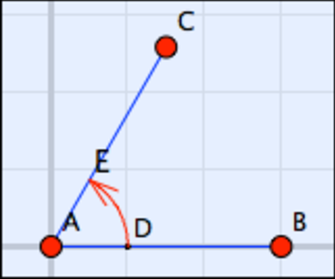
\includegraphics[width=3.5cm,bb=0 0 161 134]{Fig/setcolor.pdf}
 \\
 \\
\scalebox{0.9}{%%% colortable1-34.tex 2015-2-8 17:25
%%% colortable1-34.sce 2015-2-8 17:25
{\unitlength=1cm%
\begin{picture}%
(  15.00000,  17.50000)(  -0.00000,  -0.00000)%
\special{pn 8}%
%
\color[cmyk]{0.15,0,0.69,0}%
\settowidth{\Width}{あいうえお}\setlength{\Width}{-0.5\Width}%
\settoheight{\Height}{あいうえお}\settodepth{\Depth}{あいうえお}\setlength{\Height}{-0.5\Height}\setlength{\Depth}{0.5\Depth}\addtolength{\Height}{\Depth}%
\put(10.7500,16.7500){\hspace*{\Width}\raisebox{\Height}{あいうえお}}%
%
%
\special{pa 4626 -6693}\special{pa 4626 -6496}\special{pa 5906 -6496}\special{pa 5906 -6693}%
\special{pa 4626 -6693}\special{sh 1}\special{ip}%
\color[cmyk]{0,0,1,0}%
\settowidth{\Width}{あいうえお}\setlength{\Width}{-0.5\Width}%
\settoheight{\Height}{あいうえお}\settodepth{\Depth}{あいうえお}\setlength{\Height}{-0.5\Height}\setlength{\Depth}{0.5\Depth}\addtolength{\Height}{\Depth}%
\put(10.7500,16.2500){\hspace*{\Width}\raisebox{\Height}{あいうえお}}%
%
%
\special{pa 4626 -6496}\special{pa 4626 -6299}\special{pa 5906 -6299}\special{pa 5906 -6496}%
\special{pa 4626 -6496}\special{sh 1}\special{ip}%
\color[cmyk]{0,0.1,0.84,0}%
\settowidth{\Width}{あいうえお}\setlength{\Width}{-0.5\Width}%
\settoheight{\Height}{あいうえお}\settodepth{\Depth}{あいうえお}\setlength{\Height}{-0.5\Height}\setlength{\Depth}{0.5\Depth}\addtolength{\Height}{\Depth}%
\put(10.7500,15.7500){\hspace*{\Width}\raisebox{\Height}{あいうえお}}%
%
%
\special{pa 4626 -6299}\special{pa 4626 -6102}\special{pa 5906 -6102}\special{pa 5906 -6299}%
\special{pa 4626 -6299}\special{sh 1}\special{ip}%
\color[cmyk]{0,0.29,0.84,0}%
\settowidth{\Width}{あいうえお}\setlength{\Width}{-0.5\Width}%
\settoheight{\Height}{あいうえお}\settodepth{\Depth}{あいうえお}\setlength{\Height}{-0.5\Height}\setlength{\Depth}{0.5\Depth}\addtolength{\Height}{\Depth}%
\put(10.7500,15.2500){\hspace*{\Width}\raisebox{\Height}{あいうえお}}%
%
%
\special{pa 4626 -6102}\special{pa 4626 -5906}\special{pa 5906 -5906}\special{pa 5906 -6102}%
\special{pa 4626 -6102}\special{sh 1}\special{ip}%
\color[cmyk]{0,0.32,0.52,0}%
\settowidth{\Width}{あいうえお}\setlength{\Width}{-0.5\Width}%
\settoheight{\Height}{あいうえお}\settodepth{\Depth}{あいうえお}\setlength{\Height}{-0.5\Height}\setlength{\Depth}{0.5\Depth}\addtolength{\Height}{\Depth}%
\put(10.7500,14.7500){\hspace*{\Width}\raisebox{\Height}{あいうえお}}%
%
%
\special{pa 4626 -5906}\special{pa 4626 -5709}\special{pa 5906 -5709}\special{pa 5906 -5906}%
\special{pa 4626 -5906}\special{sh 1}\special{ip}%
\color[cmyk]{0,0.5,0.7,0}%
\settowidth{\Width}{あいうえお}\setlength{\Width}{-0.5\Width}%
\settoheight{\Height}{あいうえお}\settodepth{\Depth}{あいうえお}\setlength{\Height}{-0.5\Height}\setlength{\Depth}{0.5\Depth}\addtolength{\Height}{\Depth}%
\put(10.7500,14.2500){\hspace*{\Width}\raisebox{\Height}{あいうえお}}%
%
%
\special{pa 4626 -5709}\special{pa 4626 -5512}\special{pa 5906 -5512}\special{pa 5906 -5709}%
\special{pa 4626 -5709}\special{sh 1}\special{ip}%
\color[cmyk]{0,0.46,0.5,0}%
\settowidth{\Width}{あいうえお}\setlength{\Width}{-0.5\Width}%
\settoheight{\Height}{あいうえお}\settodepth{\Depth}{あいうえお}\setlength{\Height}{-0.5\Height}\setlength{\Depth}{0.5\Depth}\addtolength{\Height}{\Depth}%
\put(10.7500,13.7500){\hspace*{\Width}\raisebox{\Height}{あいうえお}}%
%
%
\special{pa 4626 -5512}\special{pa 4626 -5315}\special{pa 5906 -5315}\special{pa 5906 -5512}%
\special{pa 4626 -5512}\special{sh 1}\special{ip}%
\color[cmyk]{0,0.42,1,0}%
\settowidth{\Width}{あいうえお}\setlength{\Width}{-0.5\Width}%
\settoheight{\Height}{あいうえお}\settodepth{\Depth}{あいうえお}\setlength{\Height}{-0.5\Height}\setlength{\Depth}{0.5\Depth}\addtolength{\Height}{\Depth}%
\put(10.7500,13.2500){\hspace*{\Width}\raisebox{\Height}{あいうえお}}%
%
%
\special{pa 4626 -5315}\special{pa 4626 -5118}\special{pa 5906 -5118}\special{pa 5906 -5315}%
\special{pa 4626 -5315}\special{sh 1}\special{ip}%
\color[cmyk]{0,0.61,0.87,0}%
\settowidth{\Width}{あいうえお}\setlength{\Width}{-0.5\Width}%
\settoheight{\Height}{あいうえお}\settodepth{\Depth}{あいうえお}\setlength{\Height}{-0.5\Height}\setlength{\Depth}{0.5\Depth}\addtolength{\Height}{\Depth}%
\put(10.7500,12.7500){\hspace*{\Width}\raisebox{\Height}{あいうえお}}%
%
%
\special{pa 4626 -5118}\special{pa 4626 -4921}\special{pa 5906 -4921}\special{pa 5906 -5118}%
\special{pa 4626 -5118}\special{sh 1}\special{ip}%
\color[cmyk]{0,0.51,1,0}%
\settowidth{\Width}{あいうえお}\setlength{\Width}{-0.5\Width}%
\settoheight{\Height}{あいうえお}\settodepth{\Depth}{あいうえお}\setlength{\Height}{-0.5\Height}\setlength{\Depth}{0.5\Depth}\addtolength{\Height}{\Depth}%
\put(10.7500,12.2500){\hspace*{\Width}\raisebox{\Height}{あいうえお}}%
%
%
\special{pa 4626 -4921}\special{pa 4626 -4724}\special{pa 5906 -4724}\special{pa 5906 -4921}%
\special{pa 4626 -4921}\special{sh 1}\special{ip}%
\color[cmyk]{0,0.75,1,0.24}%
\settowidth{\Width}{あいうえお}\setlength{\Width}{-0.5\Width}%
\settoheight{\Height}{あいうえお}\settodepth{\Depth}{あいうえお}\setlength{\Height}{-0.5\Height}\setlength{\Depth}{0.5\Depth}\addtolength{\Height}{\Depth}%
\put(10.7500,11.7500){\hspace*{\Width}\raisebox{\Height}{あいうえお}}%
%
%
\special{pa 4626 -4724}\special{pa 4626 -4528}\special{pa 5906 -4528}\special{pa 5906 -4724}%
\special{pa 4626 -4724}\special{sh 1}\special{ip}%
\color[cmyk]{0,0.77,0.87,0}%
\settowidth{\Width}{あいうえお}\setlength{\Width}{-0.5\Width}%
\settoheight{\Height}{あいうえお}\settodepth{\Depth}{あいうえお}\setlength{\Height}{-0.5\Height}\setlength{\Depth}{0.5\Depth}\addtolength{\Height}{\Depth}%
\put(10.7500,11.2500){\hspace*{\Width}\raisebox{\Height}{あいうえお}}%
%
%
\special{pa 4626 -4528}\special{pa 4626 -4331}\special{pa 5906 -4331}\special{pa 5906 -4528}%
\special{pa 4626 -4528}\special{sh 1}\special{ip}%
\color[cmyk]{0,0.85,0.87,0.35}%
\settowidth{\Width}{あいうえお}\setlength{\Width}{-0.5\Width}%
\settoheight{\Height}{あいうえお}\settodepth{\Depth}{あいうえお}\setlength{\Height}{-0.5\Height}\setlength{\Depth}{0.5\Depth}\addtolength{\Height}{\Depth}%
\put(10.7500,10.7500){\hspace*{\Width}\raisebox{\Height}{あいうえお}}%
%
%
\special{pa 4626 -4331}\special{pa 4626 -4134}\special{pa 5906 -4134}\special{pa 5906 -4331}%
\special{pa 4626 -4331}\special{sh 1}\special{ip}%
\color[cmyk]{0,0.87,0.68,0.32}%
\settowidth{\Width}{あいうえお}\setlength{\Width}{-0.5\Width}%
\settoheight{\Height}{あいうえお}\settodepth{\Depth}{あいうえお}\setlength{\Height}{-0.5\Height}\setlength{\Depth}{0.5\Depth}\addtolength{\Height}{\Depth}%
\put(10.7500,10.2500){\hspace*{\Width}\raisebox{\Height}{あいうえお}}%
%
%
\special{pa 4626 -4134}\special{pa 4626 -3937}\special{pa 5906 -3937}\special{pa 5906 -4134}%
\special{pa 4626 -4134}\special{sh 1}\special{ip}%
\color[cmyk]{0,0.89,0.94,0.28}%
\settowidth{\Width}{あいうえお}\setlength{\Width}{-0.5\Width}%
\settoheight{\Height}{あいうえお}\settodepth{\Depth}{あいうえお}\setlength{\Height}{-0.5\Height}\setlength{\Depth}{0.5\Depth}\addtolength{\Height}{\Depth}%
\put(10.7500,9.7500){\hspace*{\Width}\raisebox{\Height}{あいうえお}}%
%
%
\special{pa 4626 -3937}\special{pa 4626 -3740}\special{pa 5906 -3740}\special{pa 5906 -3937}%
\special{pa 4626 -3937}\special{sh 1}\special{ip}%
\color[cmyk]{0,1,1,0}%
\settowidth{\Width}{あいうえお}\setlength{\Width}{-0.5\Width}%
\settoheight{\Height}{あいうえお}\settodepth{\Depth}{あいうえお}\setlength{\Height}{-0.5\Height}\setlength{\Depth}{0.5\Depth}\addtolength{\Height}{\Depth}%
\put(10.7500,9.2500){\hspace*{\Width}\raisebox{\Height}{あいうえお}}%
%
%
\special{pa 4626 -3740}\special{pa 4626 -3543}\special{pa 5906 -3543}\special{pa 5906 -3740}%
\special{pa 4626 -3740}\special{sh 1}\special{ip}%
\color[cmyk]{0,1,0.5,0}%
\settowidth{\Width}{あいうえお}\setlength{\Width}{-0.5\Width}%
\settoheight{\Height}{あいうえお}\settodepth{\Depth}{あいうえお}\setlength{\Height}{-0.5\Height}\setlength{\Depth}{0.5\Depth}\addtolength{\Height}{\Depth}%
\put(10.7500,8.7500){\hspace*{\Width}\raisebox{\Height}{あいうえお}}%
%
%
\special{pa 4626 -3543}\special{pa 4626 -3346}\special{pa 5906 -3346}\special{pa 5906 -3543}%
\special{pa 4626 -3543}\special{sh 1}\special{ip}%
\color[cmyk]{0,1,0.13,0}%
\settowidth{\Width}{あいうえお}\setlength{\Width}{-0.5\Width}%
\settoheight{\Height}{あいうえお}\settodepth{\Depth}{あいうえお}\setlength{\Height}{-0.5\Height}\setlength{\Depth}{0.5\Depth}\addtolength{\Height}{\Depth}%
\put(10.7500,8.2500){\hspace*{\Width}\raisebox{\Height}{あいうえお}}%
%
%
\special{pa 4626 -3346}\special{pa 4626 -3150}\special{pa 5906 -3150}\special{pa 5906 -3346}%
\special{pa 4626 -3346}\special{sh 1}\special{ip}%
\color[cmyk]{0,0.96,0.39,0}%
\settowidth{\Width}{あいうえお}\setlength{\Width}{-0.5\Width}%
\settoheight{\Height}{あいうえお}\settodepth{\Depth}{あいうえお}\setlength{\Height}{-0.5\Height}\setlength{\Depth}{0.5\Depth}\addtolength{\Height}{\Depth}%
\put(10.7500,7.7500){\hspace*{\Width}\raisebox{\Height}{あいうえお}}%
%
%
\special{pa 4626 -3150}\special{pa 4626 -2953}\special{pa 5906 -2953}\special{pa 5906 -3150}%
\special{pa 4626 -3150}\special{sh 1}\special{ip}%
\color[cmyk]{0,0.53,0.38,0}%
\settowidth{\Width}{あいうえお}\setlength{\Width}{-0.5\Width}%
\settoheight{\Height}{あいうえお}\settodepth{\Depth}{あいうえお}\setlength{\Height}{-0.5\Height}\setlength{\Depth}{0.5\Depth}\addtolength{\Height}{\Depth}%
\put(10.7500,7.2500){\hspace*{\Width}\raisebox{\Height}{あいうえお}}%
%
%
\special{pa 4626 -2953}\special{pa 4626 -2756}\special{pa 5906 -2756}\special{pa 5906 -2953}%
\special{pa 4626 -2953}\special{sh 1}\special{ip}%
\color[cmyk]{0,0.63,0,0}%
\settowidth{\Width}{あいうえお}\setlength{\Width}{-0.5\Width}%
\settoheight{\Height}{あいうえお}\settodepth{\Depth}{あいうえお}\setlength{\Height}{-0.5\Height}\setlength{\Depth}{0.5\Depth}\addtolength{\Height}{\Depth}%
\put(10.7500,6.7500){\hspace*{\Width}\raisebox{\Height}{あいうえお}}%
%
%
\special{pa 4626 -2756}\special{pa 4626 -2559}\special{pa 5906 -2559}\special{pa 5906 -2756}%
\special{pa 4626 -2756}\special{sh 1}\special{ip}%
\color[cmyk]{0,1,0,0}%
\settowidth{\Width}{あいうえお}\setlength{\Width}{-0.5\Width}%
\settoheight{\Height}{あいうえお}\settodepth{\Depth}{あいうえお}\setlength{\Height}{-0.5\Height}\setlength{\Depth}{0.5\Depth}\addtolength{\Height}{\Depth}%
\put(10.7500,6.2500){\hspace*{\Width}\raisebox{\Height}{あいうえお}}%
%
%
\special{pa 4626 -2559}\special{pa 4626 -2362}\special{pa 5906 -2362}\special{pa 5906 -2559}%
\special{pa 4626 -2559}\special{sh 1}\special{ip}%
\color[cmyk]{0,0.81,0,0}%
\settowidth{\Width}{あいうえお}\setlength{\Width}{-0.5\Width}%
\settoheight{\Height}{あいうえお}\settodepth{\Depth}{あいうえお}\setlength{\Height}{-0.5\Height}\setlength{\Depth}{0.5\Depth}\addtolength{\Height}{\Depth}%
\put(10.7500,5.7500){\hspace*{\Width}\raisebox{\Height}{あいうえお}}%
%
%
\special{pa 4626 -2362}\special{pa 4626 -2165}\special{pa 5906 -2165}\special{pa 5906 -2362}%
\special{pa 4626 -2362}\special{sh 1}\special{ip}%
\color[cmyk]{0,0.82,0,0}%
\settowidth{\Width}{あいうえお}\setlength{\Width}{-0.5\Width}%
\settoheight{\Height}{あいうえお}\settodepth{\Depth}{あいうえお}\setlength{\Height}{-0.5\Height}\setlength{\Depth}{0.5\Depth}\addtolength{\Height}{\Depth}%
\put(10.7500,5.2500){\hspace*{\Width}\raisebox{\Height}{あいうえお}}%
%
%
\special{pa 4626 -2165}\special{pa 4626 -1969}\special{pa 5906 -1969}\special{pa 5906 -2165}%
\special{pa 4626 -2165}\special{sh 1}\special{ip}%
\color[cmyk]{0.34,0.9,0,0.02}%
\settowidth{\Width}{あいうえお}\setlength{\Width}{-0.5\Width}%
\settoheight{\Height}{あいうえお}\settodepth{\Depth}{あいうえお}\setlength{\Height}{-0.5\Height}\setlength{\Depth}{0.5\Depth}\addtolength{\Height}{\Depth}%
\put(10.7500,4.7500){\hspace*{\Width}\raisebox{\Height}{あいうえお}}%
%
%
\special{pa 4626 -1969}\special{pa 4626 -1772}\special{pa 5906 -1772}\special{pa 5906 -1969}%
\special{pa 4626 -1969}\special{sh 1}\special{ip}%
\color[cmyk]{0.07,0.9,0,0.34}%
\settowidth{\Width}{あいうえお}\setlength{\Width}{-0.5\Width}%
\settoheight{\Height}{あいうえお}\settodepth{\Depth}{あいうえお}\setlength{\Height}{-0.5\Height}\setlength{\Depth}{0.5\Depth}\addtolength{\Height}{\Depth}%
\put(10.7500,4.2500){\hspace*{\Width}\raisebox{\Height}{あいうえお}}%
%
%
\special{pa 4626 -1772}\special{pa 4626 -1575}\special{pa 5906 -1575}\special{pa 5906 -1772}%
\special{pa 4626 -1772}\special{sh 1}\special{ip}%
\color[cmyk]{0.47,0.91,0,0.08}%
\settowidth{\Width}{あいうえお}\setlength{\Width}{-0.5\Width}%
\settoheight{\Height}{あいうえお}\settodepth{\Depth}{あいうえお}\setlength{\Height}{-0.5\Height}\setlength{\Depth}{0.5\Depth}\addtolength{\Height}{\Depth}%
\put(10.7500,3.7500){\hspace*{\Width}\raisebox{\Height}{あいうえお}}%
%
%
\special{pa 4626 -1575}\special{pa 4626 -1378}\special{pa 5906 -1378}\special{pa 5906 -1575}%
\special{pa 4626 -1575}\special{sh 1}\special{ip}%
\color[cmyk]{0,0.48,0,0}%
\settowidth{\Width}{あいうえお}\setlength{\Width}{-0.5\Width}%
\settoheight{\Height}{あいうえお}\settodepth{\Depth}{あいうえお}\setlength{\Height}{-0.5\Height}\setlength{\Depth}{0.5\Depth}\addtolength{\Height}{\Depth}%
\put(10.7500,3.2500){\hspace*{\Width}\raisebox{\Height}{あいうえお}}%
%
%
\special{pa 4626 -1378}\special{pa 4626 -1181}\special{pa 5906 -1181}\special{pa 5906 -1378}%
\special{pa 4626 -1378}\special{sh 1}\special{ip}%
\color[cmyk]{0.12,0.59,0,0}%
\settowidth{\Width}{あいうえお}\setlength{\Width}{-0.5\Width}%
\settoheight{\Height}{あいうえお}\settodepth{\Depth}{あいうえお}\setlength{\Height}{-0.5\Height}\setlength{\Depth}{0.5\Depth}\addtolength{\Height}{\Depth}%
\put(10.7500,2.7500){\hspace*{\Width}\raisebox{\Height}{あいうえお}}%
%
%
\special{pa 4626 -1181}\special{pa 4626 -984}\special{pa 5906 -984}\special{pa 5906 -1181}%
\special{pa 4626 -1181}\special{sh 1}\special{ip}%
\color[cmyk]{0.32,0.64,0,0}%
\settowidth{\Width}{あいうえお}\setlength{\Width}{-0.5\Width}%
\settoheight{\Height}{あいうえお}\settodepth{\Depth}{あいうえお}\setlength{\Height}{-0.5\Height}\setlength{\Depth}{0.5\Depth}\addtolength{\Height}{\Depth}%
\put(10.7500,2.2500){\hspace*{\Width}\raisebox{\Height}{あいうえお}}%
%
%
\special{pa 4626 -984}\special{pa 4626 -787}\special{pa 5906 -787}\special{pa 5906 -984}%
\special{pa 4626 -984}\special{sh 1}\special{ip}%
\color[cmyk]{0.4,0.8,0.2,0}%
\settowidth{\Width}{あいうえお}\setlength{\Width}{-0.5\Width}%
\settoheight{\Height}{あいうえお}\settodepth{\Depth}{あいうえお}\setlength{\Height}{-0.5\Height}\setlength{\Depth}{0.5\Depth}\addtolength{\Height}{\Depth}%
\put(10.7500,1.7500){\hspace*{\Width}\raisebox{\Height}{あいうえお}}%
%
%
\special{pa 4626 -787}\special{pa 4626 -591}\special{pa 5906 -591}\special{pa 5906 -787}%
\special{pa 4626 -787}\special{sh 1}\special{ip}%
\color[cmyk]{0.45,0.86,0,0}%
\settowidth{\Width}{あいうえお}\setlength{\Width}{-0.5\Width}%
\settoheight{\Height}{あいうえお}\settodepth{\Depth}{あいうえお}\setlength{\Height}{-0.5\Height}\setlength{\Depth}{0.5\Depth}\addtolength{\Height}{\Depth}%
\put(10.7500,1.2500){\hspace*{\Width}\raisebox{\Height}{あいうえお}}%
%
%
\special{pa 4626 -591}\special{pa 4626 -394}\special{pa 5906 -394}\special{pa 5906 -591}%
\special{pa 4626 -591}\special{sh 1}\special{ip}%
\color[cmyk]{0.5,1,0,0}%
\settowidth{\Width}{あいうえお}\setlength{\Width}{-0.5\Width}%
\settoheight{\Height}{あいうえお}\settodepth{\Depth}{あいうえお}\setlength{\Height}{-0.5\Height}\setlength{\Depth}{0.5\Depth}\addtolength{\Height}{\Depth}%
\put(10.7500,0.7500){\hspace*{\Width}\raisebox{\Height}{あいうえお}}%
%
%
\special{pa 4626 -394}\special{pa 4626 -197}\special{pa 5906 -197}\special{pa 5906 -394}%
\special{pa 4626 -394}\special{sh 1}\special{ip}%
\color[cmyk]{0.79,0.88,0,0}%
\settowidth{\Width}{あいうえお}\setlength{\Width}{-0.5\Width}%
\settoheight{\Height}{あいうえお}\settodepth{\Depth}{あいうえお}\setlength{\Height}{-0.5\Height}\setlength{\Depth}{0.5\Depth}\addtolength{\Height}{\Depth}%
\put(10.7500,0.2500){\hspace*{\Width}\raisebox{\Height}{あいうえお}}%
%
%
\special{pa 4626 -197}\special{pa 4626 0}\special{pa 5906 0}\special{pa 5906 -197}%
\special{pa 4626 -197}\special{sh 1}\special{ip}%
\color[cmyk]{0,0,0,1}%
\special{pa 0 -6890}\special{pa 1083 -6890}%
\special{fp}%
\special{pa 1083 -6890}\special{pa 2461 -6890}%
\special{fp}%
\special{pa 2461 -6890}\special{pa 3839 -6890}%
\special{fp}%
\special{pa 3839 -6890}\special{pa 4626 -6890}%
\special{fp}%
\special{pa 4626 -6890}\special{pa 5906 -6890}%
\special{fp}%
\special{pa 0 -6693}\special{pa 1083 -6693}%
\special{fp}%
\special{pa 1083 -6693}\special{pa 2461 -6693}%
\special{fp}%
\special{pa 2461 -6693}\special{pa 3839 -6693}%
\special{fp}%
\special{pa 3839 -6693}\special{pa 4626 -6693}%
\special{fp}%
\special{pa 4626 -6693}\special{pa 5906 -6693}%
\special{fp}%
\special{pa 0 -6496}\special{pa 1083 -6496}%
\special{fp}%
\special{pa 1083 -6496}\special{pa 2461 -6496}%
\special{fp}%
\special{pa 2461 -6496}\special{pa 3839 -6496}%
\special{fp}%
\special{pa 3839 -6496}\special{pa 4626 -6496}%
\special{fp}%
\special{pa 4626 -6496}\special{pa 5906 -6496}%
\special{fp}%
\special{pa 0 -6299}\special{pa 1083 -6299}%
\special{fp}%
\special{pa 1083 -6299}\special{pa 2461 -6299}%
\special{fp}%
\special{pa 2461 -6299}\special{pa 3839 -6299}%
\special{fp}%
\special{pa 3839 -6299}\special{pa 4626 -6299}%
\special{fp}%
\special{pa 4626 -6299}\special{pa 5906 -6299}%
\special{fp}%
\special{pa 0 -6102}\special{pa 1083 -6102}%
\special{fp}%
\special{pa 1083 -6102}\special{pa 2461 -6102}%
\special{fp}%
\special{pa 2461 -6102}\special{pa 3839 -6102}%
\special{fp}%
\special{pa 3839 -6102}\special{pa 4626 -6102}%
\special{fp}%
\special{pa 4626 -6102}\special{pa 5906 -6102}%
\special{fp}%
\special{pa 0 -5906}\special{pa 1083 -5906}%
\special{fp}%
\special{pa 1083 -5906}\special{pa 2461 -5906}%
\special{fp}%
\special{pa 2461 -5906}\special{pa 3839 -5906}%
\special{fp}%
\special{pa 3839 -5906}\special{pa 4626 -5906}%
\special{fp}%
\special{pa 4626 -5906}\special{pa 5906 -5906}%
\special{fp}%
\special{pa 0 -5709}\special{pa 1083 -5709}%
\special{fp}%
\special{pa 1083 -5709}\special{pa 2461 -5709}%
\special{fp}%
\special{pa 2461 -5709}\special{pa 3839 -5709}%
\special{fp}%
\special{pa 3839 -5709}\special{pa 4626 -5709}%
\special{fp}%
\special{pa 4626 -5709}\special{pa 5906 -5709}%
\special{fp}%
\special{pa 0 -5512}\special{pa 1083 -5512}%
\special{fp}%
\special{pa 1083 -5512}\special{pa 2461 -5512}%
\special{fp}%
\special{pa 2461 -5512}\special{pa 3839 -5512}%
\special{fp}%
\special{pa 3839 -5512}\special{pa 4626 -5512}%
\special{fp}%
\special{pa 4626 -5512}\special{pa 5906 -5512}%
\special{fp}%
\special{pa 0 -5315}\special{pa 1083 -5315}%
\special{fp}%
\special{pa 1083 -5315}\special{pa 2461 -5315}%
\special{fp}%
\special{pa 2461 -5315}\special{pa 3839 -5315}%
\special{fp}%
\special{pa 3839 -5315}\special{pa 4626 -5315}%
\special{fp}%
\special{pa 4626 -5315}\special{pa 5906 -5315}%
\special{fp}%
\special{pa 0 -5118}\special{pa 1083 -5118}%
\special{fp}%
\special{pa 1083 -5118}\special{pa 2461 -5118}%
\special{fp}%
\special{pa 2461 -5118}\special{pa 3839 -5118}%
\special{fp}%
\special{pa 3839 -5118}\special{pa 4626 -5118}%
\special{fp}%
\special{pa 4626 -5118}\special{pa 5906 -5118}%
\special{fp}%
\special{pa 0 -4921}\special{pa 1083 -4921}%
\special{fp}%
\special{pa 1083 -4921}\special{pa 2461 -4921}%
\special{fp}%
\special{pa 2461 -4921}\special{pa 3839 -4921}%
\special{fp}%
\special{pa 3839 -4921}\special{pa 4626 -4921}%
\special{fp}%
\special{pa 4626 -4921}\special{pa 5906 -4921}%
\special{fp}%
\special{pa 0 -4724}\special{pa 1083 -4724}%
\special{fp}%
\special{pa 1083 -4724}\special{pa 2461 -4724}%
\special{fp}%
\special{pa 2461 -4724}\special{pa 3839 -4724}%
\special{fp}%
\special{pa 3839 -4724}\special{pa 4626 -4724}%
\special{fp}%
\special{pa 4626 -4724}\special{pa 5906 -4724}%
\special{fp}%
\special{pa 0 -4528}\special{pa 1083 -4528}%
\special{fp}%
\special{pa 1083 -4528}\special{pa 2461 -4528}%
\special{fp}%
\special{pa 2461 -4528}\special{pa 3839 -4528}%
\special{fp}%
\special{pa 3839 -4528}\special{pa 4626 -4528}%
\special{fp}%
\special{pa 4626 -4528}\special{pa 5906 -4528}%
\special{fp}%
\special{pa 0 -4331}\special{pa 1083 -4331}%
\special{fp}%
\special{pa 1083 -4331}\special{pa 2461 -4331}%
\special{fp}%
\special{pa 2461 -4331}\special{pa 3839 -4331}%
\special{fp}%
\special{pa 3839 -4331}\special{pa 4626 -4331}%
\special{fp}%
\special{pa 4626 -4331}\special{pa 5906 -4331}%
\special{fp}%
\special{pa 0 -4134}\special{pa 1083 -4134}%
\special{fp}%
\special{pa 1083 -4134}\special{pa 2461 -4134}%
\special{fp}%
\special{pa 2461 -4134}\special{pa 3839 -4134}%
\special{fp}%
\special{pa 3839 -4134}\special{pa 4626 -4134}%
\special{fp}%
\special{pa 4626 -4134}\special{pa 5906 -4134}%
\special{fp}%
\special{pa 0 -3937}\special{pa 1083 -3937}%
\special{fp}%
\special{pa 1083 -3937}\special{pa 2461 -3937}%
\special{fp}%
\special{pa 2461 -3937}\special{pa 3839 -3937}%
\special{fp}%
\special{pa 3839 -3937}\special{pa 4626 -3937}%
\special{fp}%
\special{pa 4626 -3937}\special{pa 5906 -3937}%
\special{fp}%
\special{pa 0 -3740}\special{pa 1083 -3740}%
\special{fp}%
\special{pa 1083 -3740}\special{pa 2461 -3740}%
\special{fp}%
\special{pa 2461 -3740}\special{pa 3839 -3740}%
\special{fp}%
\special{pa 3839 -3740}\special{pa 4626 -3740}%
\special{fp}%
\special{pa 4626 -3740}\special{pa 5906 -3740}%
\special{fp}%
\special{pa 0 -3543}\special{pa 1083 -3543}%
\special{fp}%
\special{pa 1083 -3543}\special{pa 2461 -3543}%
\special{fp}%
\special{pa 2461 -3543}\special{pa 3839 -3543}%
\special{fp}%
\special{pa 3839 -3543}\special{pa 4626 -3543}%
\special{fp}%
\special{pa 4626 -3543}\special{pa 5906 -3543}%
\special{fp}%
\special{pa 0 -3346}\special{pa 1083 -3346}%
\special{fp}%
\special{pa 1083 -3346}\special{pa 2461 -3346}%
\special{fp}%
\special{pa 2461 -3346}\special{pa 3839 -3346}%
\special{fp}%
\special{pa 3839 -3346}\special{pa 4626 -3346}%
\special{fp}%
\special{pa 4626 -3346}\special{pa 5906 -3346}%
\special{fp}%
\special{pa 0 -3150}\special{pa 1083 -3150}%
\special{fp}%
\special{pa 1083 -3150}\special{pa 2461 -3150}%
\special{fp}%
\special{pa 2461 -3150}\special{pa 3839 -3150}%
\special{fp}%
\special{pa 3839 -3150}\special{pa 4626 -3150}%
\special{fp}%
\special{pa 4626 -3150}\special{pa 5906 -3150}%
\special{fp}%
\special{pa 0 -2953}\special{pa 1083 -2953}%
\special{fp}%
\special{pa 1083 -2953}\special{pa 2461 -2953}%
\special{fp}%
\special{pa 2461 -2953}\special{pa 3839 -2953}%
\special{fp}%
\special{pa 3839 -2953}\special{pa 4626 -2953}%
\special{fp}%
\special{pa 4626 -2953}\special{pa 5906 -2953}%
\special{fp}%
\special{pa 0 -2756}\special{pa 1083 -2756}%
\special{fp}%
\special{pa 1083 -2756}\special{pa 2461 -2756}%
\special{fp}%
\special{pa 2461 -2756}\special{pa 3839 -2756}%
\special{fp}%
\special{pa 3839 -2756}\special{pa 4626 -2756}%
\special{fp}%
\special{pa 4626 -2756}\special{pa 5906 -2756}%
\special{fp}%
\special{pa 0 -2559}\special{pa 1083 -2559}%
\special{fp}%
\special{pa 1083 -2559}\special{pa 2461 -2559}%
\special{fp}%
\special{pa 2461 -2559}\special{pa 3839 -2559}%
\special{fp}%
\special{pa 3839 -2559}\special{pa 4626 -2559}%
\special{fp}%
\special{pa 4626 -2559}\special{pa 5906 -2559}%
\special{fp}%
\special{pa 0 -2362}\special{pa 1083 -2362}%
\special{fp}%
\special{pa 1083 -2362}\special{pa 2461 -2362}%
\special{fp}%
\special{pa 2461 -2362}\special{pa 3839 -2362}%
\special{fp}%
\special{pa 3839 -2362}\special{pa 4626 -2362}%
\special{fp}%
\special{pa 4626 -2362}\special{pa 5906 -2362}%
\special{fp}%
\special{pa 0 -2165}\special{pa 1083 -2165}%
\special{fp}%
\special{pa 1083 -2165}\special{pa 2461 -2165}%
\special{fp}%
\special{pa 2461 -2165}\special{pa 3839 -2165}%
\special{fp}%
\special{pa 3839 -2165}\special{pa 4626 -2165}%
\special{fp}%
\special{pa 4626 -2165}\special{pa 5906 -2165}%
\special{fp}%
\special{pa 0 -1969}\special{pa 1083 -1969}%
\special{fp}%
\special{pa 1083 -1969}\special{pa 2461 -1969}%
\special{fp}%
\special{pa 2461 -1969}\special{pa 3839 -1969}%
\special{fp}%
\special{pa 3839 -1969}\special{pa 4626 -1969}%
\special{fp}%
\special{pa 4626 -1969}\special{pa 5906 -1969}%
\special{fp}%
\special{pa 0 -1772}\special{pa 1083 -1772}%
\special{fp}%
\special{pa 1083 -1772}\special{pa 2461 -1772}%
\special{fp}%
\special{pa 2461 -1772}\special{pa 3839 -1772}%
\special{fp}%
\special{pa 3839 -1772}\special{pa 4626 -1772}%
\special{fp}%
\special{pa 4626 -1772}\special{pa 5906 -1772}%
\special{fp}%
\special{pa 0 -1575}\special{pa 1083 -1575}%
\special{fp}%
\special{pa 1083 -1575}\special{pa 2461 -1575}%
\special{fp}%
\special{pa 2461 -1575}\special{pa 3839 -1575}%
\special{fp}%
\special{pa 3839 -1575}\special{pa 4626 -1575}%
\special{fp}%
\special{pa 4626 -1575}\special{pa 5906 -1575}%
\special{fp}%
\special{pa 0 -1378}\special{pa 1083 -1378}%
\special{fp}%
\special{pa 1083 -1378}\special{pa 2461 -1378}%
\special{fp}%
\special{pa 2461 -1378}\special{pa 3839 -1378}%
\special{fp}%
\special{pa 3839 -1378}\special{pa 4626 -1378}%
\special{fp}%
\special{pa 4626 -1378}\special{pa 5906 -1378}%
\special{fp}%
\special{pa 0 -1181}\special{pa 1083 -1181}%
\special{fp}%
\special{pa 1083 -1181}\special{pa 2461 -1181}%
\special{fp}%
\special{pa 2461 -1181}\special{pa 3839 -1181}%
\special{fp}%
\special{pa 3839 -1181}\special{pa 4626 -1181}%
\special{fp}%
\special{pa 4626 -1181}\special{pa 5906 -1181}%
\special{fp}%
\special{pa 0 -984}\special{pa 1083 -984}%
\special{fp}%
\special{pa 1083 -984}\special{pa 2461 -984}%
\special{fp}%
\special{pa 2461 -984}\special{pa 3839 -984}%
\special{fp}%
\special{pa 3839 -984}\special{pa 4626 -984}%
\special{fp}%
\special{pa 4626 -984}\special{pa 5906 -984}%
\special{fp}%
\special{pa 0 -787}\special{pa 1083 -787}%
\special{fp}%
\special{pa 1083 -787}\special{pa 2461 -787}%
\special{fp}%
\special{pa 2461 -787}\special{pa 3839 -787}%
\special{fp}%
\special{pa 3839 -787}\special{pa 4626 -787}%
\special{fp}%
\special{pa 4626 -787}\special{pa 5906 -787}%
\special{fp}%
\special{pa 0 -591}\special{pa 1083 -591}%
\special{fp}%
\special{pa 1083 -591}\special{pa 2461 -591}%
\special{fp}%
\special{pa 2461 -591}\special{pa 3839 -591}%
\special{fp}%
\special{pa 3839 -591}\special{pa 4626 -591}%
\special{fp}%
\special{pa 4626 -591}\special{pa 5906 -591}%
\special{fp}%
\special{pa 0 -394}\special{pa 1083 -394}%
\special{fp}%
\special{pa 1083 -394}\special{pa 2461 -394}%
\special{fp}%
\special{pa 2461 -394}\special{pa 3839 -394}%
\special{fp}%
\special{pa 3839 -394}\special{pa 4626 -394}%
\special{fp}%
\special{pa 4626 -394}\special{pa 5906 -394}%
\special{fp}%
\special{pa 0 -197}\special{pa 1083 -197}%
\special{fp}%
\special{pa 1083 -197}\special{pa 2461 -197}%
\special{fp}%
\special{pa 2461 -197}\special{pa 3839 -197}%
\special{fp}%
\special{pa 3839 -197}\special{pa 4626 -197}%
\special{fp}%
\special{pa 4626 -197}\special{pa 5906 -197}%
\special{fp}%
\special{pa 0 0}\special{pa 1083 0}%
\special{fp}%
\special{pa 1083 0}\special{pa 2461 0}%
\special{fp}%
\special{pa 2461 0}\special{pa 3839 0}%
\special{fp}%
\special{pa 3839 0}\special{pa 4626 0}%
\special{fp}%
\special{pa 4626 0}\special{pa 5906 0}%
\special{fp}%
\special{pa 0 -6890}\special{pa 0 -6693}%
\special{fp}%
\special{pa 0 -6693}\special{pa 0 -6496}%
\special{fp}%
\special{pa 0 -6496}\special{pa 0 -6299}%
\special{fp}%
\special{pa 0 -6299}\special{pa 0 -6102}%
\special{fp}%
\special{pa 0 -6102}\special{pa 0 -5906}%
\special{fp}%
\special{pa 0 -5906}\special{pa 0 -5709}%
\special{fp}%
\special{pa 0 -5709}\special{pa 0 -5512}%
\special{fp}%
\special{pa 0 -5512}\special{pa 0 -5315}%
\special{fp}%
\special{pa 0 -5315}\special{pa 0 -5118}%
\special{fp}%
\special{pa 0 -5118}\special{pa 0 -4921}%
\special{fp}%
\special{pa 0 -4921}\special{pa 0 -4724}%
\special{fp}%
\special{pa 0 -4724}\special{pa 0 -4528}%
\special{fp}%
\special{pa 0 -4528}\special{pa 0 -4331}%
\special{fp}%
\special{pa 0 -4331}\special{pa 0 -4134}%
\special{fp}%
\special{pa 0 -4134}\special{pa 0 -3937}%
\special{fp}%
\special{pa 0 -3937}\special{pa 0 -3740}%
\special{fp}%
\special{pa 0 -3740}\special{pa 0 -3543}%
\special{fp}%
\special{pa 0 -3543}\special{pa 0 -3346}%
\special{fp}%
\special{pa 0 -3346}\special{pa 0 -3150}%
\special{fp}%
\special{pa 0 -3150}\special{pa 0 -2953}%
\special{fp}%
\special{pa 0 -2953}\special{pa 0 -2756}%
\special{fp}%
\special{pa 0 -2756}\special{pa 0 -2559}%
\special{fp}%
\special{pa 0 -2559}\special{pa 0 -2362}%
\special{fp}%
\special{pa 0 -2362}\special{pa 0 -2165}%
\special{fp}%
\special{pa 0 -2165}\special{pa 0 -1969}%
\special{fp}%
\special{pa 0 -1969}\special{pa 0 -1772}%
\special{fp}%
\special{pa 0 -1772}\special{pa 0 -1575}%
\special{fp}%
\special{pa 0 -1575}\special{pa 0 -1378}%
\special{fp}%
\special{pa 0 -1378}\special{pa 0 -1181}%
\special{fp}%
\special{pa 0 -1181}\special{pa 0 -984}%
\special{fp}%
\special{pa 0 -984}\special{pa 0 -787}%
\special{fp}%
\special{pa 0 -787}\special{pa 0 -591}%
\special{fp}%
\special{pa 0 -591}\special{pa 0 -394}%
\special{fp}%
\special{pa 0 -394}\special{pa 0 -197}%
\special{fp}%
\special{pa 0 -197}\special{pa 0 0}%
\special{fp}%
\special{pa 1083 -6890}\special{pa 1083 -6693}%
\special{fp}%
\special{pa 1083 -6693}\special{pa 1083 -6496}%
\special{fp}%
\special{pa 1083 -6496}\special{pa 1083 -6299}%
\special{fp}%
\special{pa 1083 -6299}\special{pa 1083 -6102}%
\special{fp}%
\special{pa 1083 -6102}\special{pa 1083 -5906}%
\special{fp}%
\special{pa 1083 -5906}\special{pa 1083 -5709}%
\special{fp}%
\special{pa 1083 -5709}\special{pa 1083 -5512}%
\special{fp}%
\special{pa 1083 -5512}\special{pa 1083 -5315}%
\special{fp}%
\special{pa 1083 -5315}\special{pa 1083 -5118}%
\special{fp}%
\special{pa 1083 -5118}\special{pa 1083 -4921}%
\special{fp}%
\special{pa 1083 -4921}\special{pa 1083 -4724}%
\special{fp}%
\special{pa 1083 -4724}\special{pa 1083 -4528}%
\special{fp}%
\special{pa 1083 -4528}\special{pa 1083 -4331}%
\special{fp}%
\special{pa 1083 -4331}\special{pa 1083 -4134}%
\special{fp}%
\special{pa 1083 -4134}\special{pa 1083 -3937}%
\special{fp}%
\special{pa 1083 -3937}\special{pa 1083 -3740}%
\special{fp}%
\special{pa 1083 -3740}\special{pa 1083 -3543}%
\special{fp}%
\special{pa 1083 -3543}\special{pa 1083 -3346}%
\special{fp}%
\special{pa 1083 -3346}\special{pa 1083 -3150}%
\special{fp}%
\special{pa 1083 -3150}\special{pa 1083 -2953}%
\special{fp}%
\special{pa 1083 -2953}\special{pa 1083 -2756}%
\special{fp}%
\special{pa 1083 -2756}\special{pa 1083 -2559}%
\special{fp}%
\special{pa 1083 -2559}\special{pa 1083 -2362}%
\special{fp}%
\special{pa 1083 -2362}\special{pa 1083 -2165}%
\special{fp}%
\special{pa 1083 -2165}\special{pa 1083 -1969}%
\special{fp}%
\special{pa 1083 -1969}\special{pa 1083 -1772}%
\special{fp}%
\special{pa 1083 -1772}\special{pa 1083 -1575}%
\special{fp}%
\special{pa 1083 -1575}\special{pa 1083 -1378}%
\special{fp}%
\special{pa 1083 -1378}\special{pa 1083 -1181}%
\special{fp}%
\special{pa 1083 -1181}\special{pa 1083 -984}%
\special{fp}%
\special{pa 1083 -984}\special{pa 1083 -787}%
\special{fp}%
\special{pa 1083 -787}\special{pa 1083 -591}%
\special{fp}%
\special{pa 1083 -591}\special{pa 1083 -394}%
\special{fp}%
\special{pa 1083 -394}\special{pa 1083 -197}%
\special{fp}%
\special{pa 1083 -197}\special{pa 1083 0}%
\special{fp}%
\special{pa 2461 -6890}\special{pa 2461 -6693}%
\special{fp}%
\special{pa 2461 -6693}\special{pa 2461 -6496}%
\special{fp}%
\special{pa 2461 -6496}\special{pa 2461 -6299}%
\special{fp}%
\special{pa 2461 -6299}\special{pa 2461 -6102}%
\special{fp}%
\special{pa 2461 -6102}\special{pa 2461 -5906}%
\special{fp}%
\special{pa 2461 -5906}\special{pa 2461 -5709}%
\special{fp}%
\special{pa 2461 -5709}\special{pa 2461 -5512}%
\special{fp}%
\special{pa 2461 -5512}\special{pa 2461 -5315}%
\special{fp}%
\special{pa 2461 -5315}\special{pa 2461 -5118}%
\special{fp}%
\special{pa 2461 -5118}\special{pa 2461 -4921}%
\special{fp}%
\special{pa 2461 -4921}\special{pa 2461 -4724}%
\special{fp}%
\special{pa 2461 -4724}\special{pa 2461 -4528}%
\special{fp}%
\special{pa 2461 -4528}\special{pa 2461 -4331}%
\special{fp}%
\special{pa 2461 -4331}\special{pa 2461 -4134}%
\special{fp}%
\special{pa 2461 -4134}\special{pa 2461 -3937}%
\special{fp}%
\special{pa 2461 -3937}\special{pa 2461 -3740}%
\special{fp}%
\special{pa 2461 -3740}\special{pa 2461 -3543}%
\special{fp}%
\special{pa 2461 -3543}\special{pa 2461 -3346}%
\special{fp}%
\special{pa 2461 -3346}\special{pa 2461 -3150}%
\special{fp}%
\special{pa 2461 -3150}\special{pa 2461 -2953}%
\special{fp}%
\special{pa 2461 -2953}\special{pa 2461 -2756}%
\special{fp}%
\special{pa 2461 -2756}\special{pa 2461 -2559}%
\special{fp}%
\special{pa 2461 -2559}\special{pa 2461 -2362}%
\special{fp}%
\special{pa 2461 -2362}\special{pa 2461 -2165}%
\special{fp}%
\special{pa 2461 -2165}\special{pa 2461 -1969}%
\special{fp}%
\special{pa 2461 -1969}\special{pa 2461 -1772}%
\special{fp}%
\special{pa 2461 -1772}\special{pa 2461 -1575}%
\special{fp}%
\special{pa 2461 -1575}\special{pa 2461 -1378}%
\special{fp}%
\special{pa 2461 -1378}\special{pa 2461 -1181}%
\special{fp}%
\special{pa 2461 -1181}\special{pa 2461 -984}%
\special{fp}%
\special{pa 2461 -984}\special{pa 2461 -787}%
\special{fp}%
\special{pa 2461 -787}\special{pa 2461 -591}%
\special{fp}%
\special{pa 2461 -591}\special{pa 2461 -394}%
\special{fp}%
\special{pa 2461 -394}\special{pa 2461 -197}%
\special{fp}%
\special{pa 2461 -197}\special{pa 2461 0}%
\special{fp}%
\special{pa 3839 -6890}\special{pa 3839 -6693}%
\special{fp}%
\special{pa 3839 -6693}\special{pa 3839 -6496}%
\special{fp}%
\special{pa 3839 -6496}\special{pa 3839 -6299}%
\special{fp}%
\special{pa 3839 -6299}\special{pa 3839 -6102}%
\special{fp}%
\special{pa 3839 -6102}\special{pa 3839 -5906}%
\special{fp}%
\special{pa 3839 -5906}\special{pa 3839 -5709}%
\special{fp}%
\special{pa 3839 -5709}\special{pa 3839 -5512}%
\special{fp}%
\special{pa 3839 -5512}\special{pa 3839 -5315}%
\special{fp}%
\special{pa 3839 -5315}\special{pa 3839 -5118}%
\special{fp}%
\special{pa 3839 -5118}\special{pa 3839 -4921}%
\special{fp}%
\special{pa 3839 -4921}\special{pa 3839 -4724}%
\special{fp}%
\special{pa 3839 -4724}\special{pa 3839 -4528}%
\special{fp}%
\special{pa 3839 -4528}\special{pa 3839 -4331}%
\special{fp}%
\special{pa 3839 -4331}\special{pa 3839 -4134}%
\special{fp}%
\special{pa 3839 -4134}\special{pa 3839 -3937}%
\special{fp}%
\special{pa 3839 -3937}\special{pa 3839 -3740}%
\special{fp}%
\special{pa 3839 -3740}\special{pa 3839 -3543}%
\special{fp}%
\special{pa 3839 -3543}\special{pa 3839 -3346}%
\special{fp}%
\special{pa 3839 -3346}\special{pa 3839 -3150}%
\special{fp}%
\special{pa 3839 -3150}\special{pa 3839 -2953}%
\special{fp}%
\special{pa 3839 -2953}\special{pa 3839 -2756}%
\special{fp}%
\special{pa 3839 -2756}\special{pa 3839 -2559}%
\special{fp}%
\special{pa 3839 -2559}\special{pa 3839 -2362}%
\special{fp}%
\special{pa 3839 -2362}\special{pa 3839 -2165}%
\special{fp}%
\special{pa 3839 -2165}\special{pa 3839 -1969}%
\special{fp}%
\special{pa 3839 -1969}\special{pa 3839 -1772}%
\special{fp}%
\special{pa 3839 -1772}\special{pa 3839 -1575}%
\special{fp}%
\special{pa 3839 -1575}\special{pa 3839 -1378}%
\special{fp}%
\special{pa 3839 -1378}\special{pa 3839 -1181}%
\special{fp}%
\special{pa 3839 -1181}\special{pa 3839 -984}%
\special{fp}%
\special{pa 3839 -984}\special{pa 3839 -787}%
\special{fp}%
\special{pa 3839 -787}\special{pa 3839 -591}%
\special{fp}%
\special{pa 3839 -591}\special{pa 3839 -394}%
\special{fp}%
\special{pa 3839 -394}\special{pa 3839 -197}%
\special{fp}%
\special{pa 3839 -197}\special{pa 3839 0}%
\special{fp}%
\special{pa 4626 -6890}\special{pa 4626 -6693}%
\special{fp}%
\special{pa 4626 -6693}\special{pa 4626 -6496}%
\special{fp}%
\special{pa 4626 -6496}\special{pa 4626 -6299}%
\special{fp}%
\special{pa 4626 -6299}\special{pa 4626 -6102}%
\special{fp}%
\special{pa 4626 -6102}\special{pa 4626 -5906}%
\special{fp}%
\special{pa 4626 -5906}\special{pa 4626 -5709}%
\special{fp}%
\special{pa 4626 -5709}\special{pa 4626 -5512}%
\special{fp}%
\special{pa 4626 -5512}\special{pa 4626 -5315}%
\special{fp}%
\special{pa 4626 -5315}\special{pa 4626 -5118}%
\special{fp}%
\special{pa 4626 -5118}\special{pa 4626 -4921}%
\special{fp}%
\special{pa 4626 -4921}\special{pa 4626 -4724}%
\special{fp}%
\special{pa 4626 -4724}\special{pa 4626 -4528}%
\special{fp}%
\special{pa 4626 -4528}\special{pa 4626 -4331}%
\special{fp}%
\special{pa 4626 -4331}\special{pa 4626 -4134}%
\special{fp}%
\special{pa 4626 -4134}\special{pa 4626 -3937}%
\special{fp}%
\special{pa 4626 -3937}\special{pa 4626 -3740}%
\special{fp}%
\special{pa 4626 -3740}\special{pa 4626 -3543}%
\special{fp}%
\special{pa 4626 -3543}\special{pa 4626 -3346}%
\special{fp}%
\special{pa 4626 -3346}\special{pa 4626 -3150}%
\special{fp}%
\special{pa 4626 -3150}\special{pa 4626 -2953}%
\special{fp}%
\special{pa 4626 -2953}\special{pa 4626 -2756}%
\special{fp}%
\special{pa 4626 -2756}\special{pa 4626 -2559}%
\special{fp}%
\special{pa 4626 -2559}\special{pa 4626 -2362}%
\special{fp}%
\special{pa 4626 -2362}\special{pa 4626 -2165}%
\special{fp}%
\special{pa 4626 -2165}\special{pa 4626 -1969}%
\special{fp}%
\special{pa 4626 -1969}\special{pa 4626 -1772}%
\special{fp}%
\special{pa 4626 -1772}\special{pa 4626 -1575}%
\special{fp}%
\special{pa 4626 -1575}\special{pa 4626 -1378}%
\special{fp}%
\special{pa 4626 -1378}\special{pa 4626 -1181}%
\special{fp}%
\special{pa 4626 -1181}\special{pa 4626 -984}%
\special{fp}%
\special{pa 4626 -984}\special{pa 4626 -787}%
\special{fp}%
\special{pa 4626 -787}\special{pa 4626 -591}%
\special{fp}%
\special{pa 4626 -591}\special{pa 4626 -394}%
\special{fp}%
\special{pa 4626 -394}\special{pa 4626 -197}%
\special{fp}%
\special{pa 4626 -197}\special{pa 4626 0}%
\special{fp}%
\special{pa 5906 -6890}\special{pa 5906 -6693}%
\special{fp}%
\special{pa 5906 -6693}\special{pa 5906 -6496}%
\special{fp}%
\special{pa 5906 -6496}\special{pa 5906 -6299}%
\special{fp}%
\special{pa 5906 -6299}\special{pa 5906 -6102}%
\special{fp}%
\special{pa 5906 -6102}\special{pa 5906 -5906}%
\special{fp}%
\special{pa 5906 -5906}\special{pa 5906 -5709}%
\special{fp}%
\special{pa 5906 -5709}\special{pa 5906 -5512}%
\special{fp}%
\special{pa 5906 -5512}\special{pa 5906 -5315}%
\special{fp}%
\special{pa 5906 -5315}\special{pa 5906 -5118}%
\special{fp}%
\special{pa 5906 -5118}\special{pa 5906 -4921}%
\special{fp}%
\special{pa 5906 -4921}\special{pa 5906 -4724}%
\special{fp}%
\special{pa 5906 -4724}\special{pa 5906 -4528}%
\special{fp}%
\special{pa 5906 -4528}\special{pa 5906 -4331}%
\special{fp}%
\special{pa 5906 -4331}\special{pa 5906 -4134}%
\special{fp}%
\special{pa 5906 -4134}\special{pa 5906 -3937}%
\special{fp}%
\special{pa 5906 -3937}\special{pa 5906 -3740}%
\special{fp}%
\special{pa 5906 -3740}\special{pa 5906 -3543}%
\special{fp}%
\special{pa 5906 -3543}\special{pa 5906 -3346}%
\special{fp}%
\special{pa 5906 -3346}\special{pa 5906 -3150}%
\special{fp}%
\special{pa 5906 -3150}\special{pa 5906 -2953}%
\special{fp}%
\special{pa 5906 -2953}\special{pa 5906 -2756}%
\special{fp}%
\special{pa 5906 -2756}\special{pa 5906 -2559}%
\special{fp}%
\special{pa 5906 -2559}\special{pa 5906 -2362}%
\special{fp}%
\special{pa 5906 -2362}\special{pa 5906 -2165}%
\special{fp}%
\special{pa 5906 -2165}\special{pa 5906 -1969}%
\special{fp}%
\special{pa 5906 -1969}\special{pa 5906 -1772}%
\special{fp}%
\special{pa 5906 -1772}\special{pa 5906 -1575}%
\special{fp}%
\special{pa 5906 -1575}\special{pa 5906 -1378}%
\special{fp}%
\special{pa 5906 -1378}\special{pa 5906 -1181}%
\special{fp}%
\special{pa 5906 -1181}\special{pa 5906 -984}%
\special{fp}%
\special{pa 5906 -984}\special{pa 5906 -787}%
\special{fp}%
\special{pa 5906 -787}\special{pa 5906 -591}%
\special{fp}%
\special{pa 5906 -591}\special{pa 5906 -394}%
\special{fp}%
\special{pa 5906 -394}\special{pa 5906 -197}%
\special{fp}%
\special{pa 5906 -197}\special{pa 5906 0}%
\special{fp}%
\settowidth{\Width}{色の名前(和名)}\setlength{\Width}{-0.5\Width}%
\settoheight{\Height}{色の名前(和名)}\settodepth{\Depth}{色の名前(和名)}\setlength{\Height}{-0.5\Height}\setlength{\Depth}{0.5\Depth}\addtolength{\Height}{\Depth}%
\put(1.3800,17.2500){\hspace*{\Width}\raisebox{\Height}{色の名前(和名)}}%
%
%
\settowidth{\Width}{\TeX コマンド(英語)}\setlength{\Width}{-0.5\Width}%
\settoheight{\Height}{\TeX コマンド(英語)}\settodepth{\Depth}{\TeX コマンド(英語)}\setlength{\Height}{-0.5\Height}\setlength{\Depth}{0.5\Depth}\addtolength{\Height}{\Depth}%
\put(4.5000,17.2500){\hspace*{\Width}\raisebox{\Height}{\TeX コマンド(英語)}}%
%
%
\settowidth{\Width}{[C,M,Y,K]のベクトル}\setlength{\Width}{-0.5\Width}%
\settoheight{\Height}{[C,M,Y,K]のベクトル}\settodepth{\Depth}{[C,M,Y,K]のベクトル}\setlength{\Height}{-0.5\Height}\setlength{\Depth}{0.5\Depth}\addtolength{\Height}{\Depth}%
\put(8.0000,17.2500){\hspace*{\Width}\raisebox{\Height}{[C,M,Y,K]のベクトル}}%
%
%
\settowidth{\Width}{文字(例)}\setlength{\Width}{-0.5\Width}%
\settoheight{\Height}{文字(例)}\settodepth{\Depth}{文字(例)}\setlength{\Height}{-0.5\Height}\setlength{\Depth}{0.5\Depth}\addtolength{\Height}{\Depth}%
\put(10.7500,17.2500){\hspace*{\Width}\raisebox{\Height}{文字(例)}}%
%
%
\settowidth{\Width}{塗りつぶし(濃さ1)}\setlength{\Width}{-0.5\Width}%
\settoheight{\Height}{塗りつぶし(濃さ1)}\settodepth{\Depth}{塗りつぶし(濃さ1)}\setlength{\Height}{-0.5\Height}\setlength{\Depth}{0.5\Depth}\addtolength{\Height}{\Depth}%
\put(13.3800,17.2500){\hspace*{\Width}\raisebox{\Height}{塗りつぶし(濃さ1)}}%
%
%
\settowidth{\Width}{}\setlength{\Width}{-0.5\Width}%
\settoheight{\Height}{}\settodepth{\Depth}{}\setlength{\Height}{-0.5\Height}\setlength{\Depth}{0.5\Depth}\addtolength{\Height}{\Depth}%
\put(1.3800,16.7500){\hspace*{\Width}\raisebox{\Height}{}}%
%
%
\settowidth{\Width}{greenyellow}\setlength{\Width}{-0.5\Width}%
\settoheight{\Height}{greenyellow}\settodepth{\Depth}{greenyellow}\setlength{\Height}{-0.5\Height}\setlength{\Depth}{0.5\Depth}\addtolength{\Height}{\Depth}%
\put(4.5000,16.7500){\hspace*{\Width}\raisebox{\Height}{greenyellow}}%
%
%
\settowidth{\Width}{[0.15,0,0.69,0]}\setlength{\Width}{-0.5\Width}%
\settoheight{\Height}{[0.15,0,0.69,0]}\settodepth{\Depth}{[0.15,0,0.69,0]}\setlength{\Height}{-0.5\Height}\setlength{\Depth}{0.5\Depth}\addtolength{\Height}{\Depth}%
\put(8.0000,16.7500){\hspace*{\Width}\raisebox{\Height}{[0.15,0,0.69,0]}}%
%
%
\settowidth{\Width}{}\setlength{\Width}{-0.5\Width}%
\settoheight{\Height}{}\settodepth{\Depth}{}\setlength{\Height}{-0.5\Height}\setlength{\Depth}{0.5\Depth}\addtolength{\Height}{\Depth}%
\put(10.7500,16.7500){\hspace*{\Width}\raisebox{\Height}{}}%
%
%
\settowidth{\Width}{}\setlength{\Width}{-0.5\Width}%
\settoheight{\Height}{}\settodepth{\Depth}{}\setlength{\Height}{-0.5\Height}\setlength{\Depth}{0.5\Depth}\addtolength{\Height}{\Depth}%
\put(13.3800,16.7500){\hspace*{\Width}\raisebox{\Height}{}}%
%
%
\settowidth{\Width}{黄色}\setlength{\Width}{-0.5\Width}%
\settoheight{\Height}{黄色}\settodepth{\Depth}{黄色}\setlength{\Height}{-0.5\Height}\setlength{\Depth}{0.5\Depth}\addtolength{\Height}{\Depth}%
\put(1.3800,16.2500){\hspace*{\Width}\raisebox{\Height}{黄色}}%
%
%
\settowidth{\Width}{yellow}\setlength{\Width}{-0.5\Width}%
\settoheight{\Height}{yellow}\settodepth{\Depth}{yellow}\setlength{\Height}{-0.5\Height}\setlength{\Depth}{0.5\Depth}\addtolength{\Height}{\Depth}%
\put(4.5000,16.2500){\hspace*{\Width}\raisebox{\Height}{yellow}}%
%
%
\settowidth{\Width}{[0,0,1,0]}\setlength{\Width}{-0.5\Width}%
\settoheight{\Height}{[0,0,1,0]}\settodepth{\Depth}{[0,0,1,0]}\setlength{\Height}{-0.5\Height}\setlength{\Depth}{0.5\Depth}\addtolength{\Height}{\Depth}%
\put(8.0000,16.2500){\hspace*{\Width}\raisebox{\Height}{[0,0,1,0]}}%
%
%
\settowidth{\Width}{}\setlength{\Width}{-0.5\Width}%
\settoheight{\Height}{}\settodepth{\Depth}{}\setlength{\Height}{-0.5\Height}\setlength{\Depth}{0.5\Depth}\addtolength{\Height}{\Depth}%
\put(10.7500,16.2500){\hspace*{\Width}\raisebox{\Height}{}}%
%
%
\settowidth{\Width}{}\setlength{\Width}{-0.5\Width}%
\settoheight{\Height}{}\settodepth{\Depth}{}\setlength{\Height}{-0.5\Height}\setlength{\Depth}{0.5\Depth}\addtolength{\Height}{\Depth}%
\put(13.3800,16.2500){\hspace*{\Width}\raisebox{\Height}{}}%
%
%
\settowidth{\Width}{}\setlength{\Width}{-0.5\Width}%
\settoheight{\Height}{}\settodepth{\Depth}{}\setlength{\Height}{-0.5\Height}\setlength{\Depth}{0.5\Depth}\addtolength{\Height}{\Depth}%
\put(1.3800,15.7500){\hspace*{\Width}\raisebox{\Height}{}}%
%
%
\settowidth{\Width}{goldenrod}\setlength{\Width}{-0.5\Width}%
\settoheight{\Height}{goldenrod}\settodepth{\Depth}{goldenrod}\setlength{\Height}{-0.5\Height}\setlength{\Depth}{0.5\Depth}\addtolength{\Height}{\Depth}%
\put(4.5000,15.7500){\hspace*{\Width}\raisebox{\Height}{goldenrod}}%
%
%
\settowidth{\Width}{[0,0.1,0.84,0]}\setlength{\Width}{-0.5\Width}%
\settoheight{\Height}{[0,0.1,0.84,0]}\settodepth{\Depth}{[0,0.1,0.84,0]}\setlength{\Height}{-0.5\Height}\setlength{\Depth}{0.5\Depth}\addtolength{\Height}{\Depth}%
\put(8.0000,15.7500){\hspace*{\Width}\raisebox{\Height}{[0,0.1,0.84,0]}}%
%
%
\settowidth{\Width}{}\setlength{\Width}{-0.5\Width}%
\settoheight{\Height}{}\settodepth{\Depth}{}\setlength{\Height}{-0.5\Height}\setlength{\Depth}{0.5\Depth}\addtolength{\Height}{\Depth}%
\put(10.7500,15.7500){\hspace*{\Width}\raisebox{\Height}{}}%
%
%
\settowidth{\Width}{}\setlength{\Width}{-0.5\Width}%
\settoheight{\Height}{}\settodepth{\Depth}{}\setlength{\Height}{-0.5\Height}\setlength{\Depth}{0.5\Depth}\addtolength{\Height}{\Depth}%
\put(13.3800,15.7500){\hspace*{\Width}\raisebox{\Height}{}}%
%
%
\settowidth{\Width}{}\setlength{\Width}{-0.5\Width}%
\settoheight{\Height}{}\settodepth{\Depth}{}\setlength{\Height}{-0.5\Height}\setlength{\Depth}{0.5\Depth}\addtolength{\Height}{\Depth}%
\put(1.3800,15.2500){\hspace*{\Width}\raisebox{\Height}{}}%
%
%
\settowidth{\Width}{dandelion}\setlength{\Width}{-0.5\Width}%
\settoheight{\Height}{dandelion}\settodepth{\Depth}{dandelion}\setlength{\Height}{-0.5\Height}\setlength{\Depth}{0.5\Depth}\addtolength{\Height}{\Depth}%
\put(4.5000,15.2500){\hspace*{\Width}\raisebox{\Height}{dandelion}}%
%
%
\settowidth{\Width}{[0,0.29,0.84,0]}\setlength{\Width}{-0.5\Width}%
\settoheight{\Height}{[0,0.29,0.84,0]}\settodepth{\Depth}{[0,0.29,0.84,0]}\setlength{\Height}{-0.5\Height}\setlength{\Depth}{0.5\Depth}\addtolength{\Height}{\Depth}%
\put(8.0000,15.2500){\hspace*{\Width}\raisebox{\Height}{[0,0.29,0.84,0]}}%
%
%
\settowidth{\Width}{}\setlength{\Width}{-0.5\Width}%
\settoheight{\Height}{}\settodepth{\Depth}{}\setlength{\Height}{-0.5\Height}\setlength{\Depth}{0.5\Depth}\addtolength{\Height}{\Depth}%
\put(10.7500,15.2500){\hspace*{\Width}\raisebox{\Height}{}}%
%
%
\settowidth{\Width}{}\setlength{\Width}{-0.5\Width}%
\settoheight{\Height}{}\settodepth{\Depth}{}\setlength{\Height}{-0.5\Height}\setlength{\Depth}{0.5\Depth}\addtolength{\Height}{\Depth}%
\put(13.3800,15.2500){\hspace*{\Width}\raisebox{\Height}{}}%
%
%
\settowidth{\Width}{}\setlength{\Width}{-0.5\Width}%
\settoheight{\Height}{}\settodepth{\Depth}{}\setlength{\Height}{-0.5\Height}\setlength{\Depth}{0.5\Depth}\addtolength{\Height}{\Depth}%
\put(1.3800,14.7500){\hspace*{\Width}\raisebox{\Height}{}}%
%
%
\settowidth{\Width}{apricot}\setlength{\Width}{-0.5\Width}%
\settoheight{\Height}{apricot}\settodepth{\Depth}{apricot}\setlength{\Height}{-0.5\Height}\setlength{\Depth}{0.5\Depth}\addtolength{\Height}{\Depth}%
\put(4.5000,14.7500){\hspace*{\Width}\raisebox{\Height}{apricot}}%
%
%
\settowidth{\Width}{[0,0.32,0.52,0]}\setlength{\Width}{-0.5\Width}%
\settoheight{\Height}{[0,0.32,0.52,0]}\settodepth{\Depth}{[0,0.32,0.52,0]}\setlength{\Height}{-0.5\Height}\setlength{\Depth}{0.5\Depth}\addtolength{\Height}{\Depth}%
\put(8.0000,14.7500){\hspace*{\Width}\raisebox{\Height}{[0,0.32,0.52,0]}}%
%
%
\settowidth{\Width}{}\setlength{\Width}{-0.5\Width}%
\settoheight{\Height}{}\settodepth{\Depth}{}\setlength{\Height}{-0.5\Height}\setlength{\Depth}{0.5\Depth}\addtolength{\Height}{\Depth}%
\put(10.7500,14.7500){\hspace*{\Width}\raisebox{\Height}{}}%
%
%
\settowidth{\Width}{}\setlength{\Width}{-0.5\Width}%
\settoheight{\Height}{}\settodepth{\Depth}{}\setlength{\Height}{-0.5\Height}\setlength{\Depth}{0.5\Depth}\addtolength{\Height}{\Depth}%
\put(13.3800,14.7500){\hspace*{\Width}\raisebox{\Height}{}}%
%
%
\settowidth{\Width}{}\setlength{\Width}{-0.5\Width}%
\settoheight{\Height}{}\settodepth{\Depth}{}\setlength{\Height}{-0.5\Height}\setlength{\Depth}{0.5\Depth}\addtolength{\Height}{\Depth}%
\put(1.3800,14.2500){\hspace*{\Width}\raisebox{\Height}{}}%
%
%
\settowidth{\Width}{peach}\setlength{\Width}{-0.5\Width}%
\settoheight{\Height}{peach}\settodepth{\Depth}{peach}\setlength{\Height}{-0.5\Height}\setlength{\Depth}{0.5\Depth}\addtolength{\Height}{\Depth}%
\put(4.5000,14.2500){\hspace*{\Width}\raisebox{\Height}{peach}}%
%
%
\settowidth{\Width}{[0,0.5,0.7,0]}\setlength{\Width}{-0.5\Width}%
\settoheight{\Height}{[0,0.5,0.7,0]}\settodepth{\Depth}{[0,0.5,0.7,0]}\setlength{\Height}{-0.5\Height}\setlength{\Depth}{0.5\Depth}\addtolength{\Height}{\Depth}%
\put(8.0000,14.2500){\hspace*{\Width}\raisebox{\Height}{[0,0.5,0.7,0]}}%
%
%
\settowidth{\Width}{}\setlength{\Width}{-0.5\Width}%
\settoheight{\Height}{}\settodepth{\Depth}{}\setlength{\Height}{-0.5\Height}\setlength{\Depth}{0.5\Depth}\addtolength{\Height}{\Depth}%
\put(10.7500,14.2500){\hspace*{\Width}\raisebox{\Height}{}}%
%
%
\settowidth{\Width}{}\setlength{\Width}{-0.5\Width}%
\settoheight{\Height}{}\settodepth{\Depth}{}\setlength{\Height}{-0.5\Height}\setlength{\Depth}{0.5\Depth}\addtolength{\Height}{\Depth}%
\put(13.3800,14.2500){\hspace*{\Width}\raisebox{\Height}{}}%
%
%
\settowidth{\Width}{}\setlength{\Width}{-0.5\Width}%
\settoheight{\Height}{}\settodepth{\Depth}{}\setlength{\Height}{-0.5\Height}\setlength{\Depth}{0.5\Depth}\addtolength{\Height}{\Depth}%
\put(1.3800,13.7500){\hspace*{\Width}\raisebox{\Height}{}}%
%
%
\settowidth{\Width}{melon}\setlength{\Width}{-0.5\Width}%
\settoheight{\Height}{melon}\settodepth{\Depth}{melon}\setlength{\Height}{-0.5\Height}\setlength{\Depth}{0.5\Depth}\addtolength{\Height}{\Depth}%
\put(4.5000,13.7500){\hspace*{\Width}\raisebox{\Height}{melon}}%
%
%
\settowidth{\Width}{[0,0.46,0.5,0]}\setlength{\Width}{-0.5\Width}%
\settoheight{\Height}{[0,0.46,0.5,0]}\settodepth{\Depth}{[0,0.46,0.5,0]}\setlength{\Height}{-0.5\Height}\setlength{\Depth}{0.5\Depth}\addtolength{\Height}{\Depth}%
\put(8.0000,13.7500){\hspace*{\Width}\raisebox{\Height}{[0,0.46,0.5,0]}}%
%
%
\settowidth{\Width}{}\setlength{\Width}{-0.5\Width}%
\settoheight{\Height}{}\settodepth{\Depth}{}\setlength{\Height}{-0.5\Height}\setlength{\Depth}{0.5\Depth}\addtolength{\Height}{\Depth}%
\put(10.7500,13.7500){\hspace*{\Width}\raisebox{\Height}{}}%
%
%
\settowidth{\Width}{}\setlength{\Width}{-0.5\Width}%
\settoheight{\Height}{}\settodepth{\Depth}{}\setlength{\Height}{-0.5\Height}\setlength{\Depth}{0.5\Depth}\addtolength{\Height}{\Depth}%
\put(13.3800,13.7500){\hspace*{\Width}\raisebox{\Height}{}}%
%
%
\settowidth{\Width}{}\setlength{\Width}{-0.5\Width}%
\settoheight{\Height}{}\settodepth{\Depth}{}\setlength{\Height}{-0.5\Height}\setlength{\Depth}{0.5\Depth}\addtolength{\Height}{\Depth}%
\put(1.3800,13.2500){\hspace*{\Width}\raisebox{\Height}{}}%
%
%
\settowidth{\Width}{yelloworange}\setlength{\Width}{-0.5\Width}%
\settoheight{\Height}{yelloworange}\settodepth{\Depth}{yelloworange}\setlength{\Height}{-0.5\Height}\setlength{\Depth}{0.5\Depth}\addtolength{\Height}{\Depth}%
\put(4.5000,13.2500){\hspace*{\Width}\raisebox{\Height}{yelloworange}}%
%
%
\settowidth{\Width}{[0,0.42,1,0]}\setlength{\Width}{-0.5\Width}%
\settoheight{\Height}{[0,0.42,1,0]}\settodepth{\Depth}{[0,0.42,1,0]}\setlength{\Height}{-0.5\Height}\setlength{\Depth}{0.5\Depth}\addtolength{\Height}{\Depth}%
\put(8.0000,13.2500){\hspace*{\Width}\raisebox{\Height}{[0,0.42,1,0]}}%
%
%
\settowidth{\Width}{}\setlength{\Width}{-0.5\Width}%
\settoheight{\Height}{}\settodepth{\Depth}{}\setlength{\Height}{-0.5\Height}\setlength{\Depth}{0.5\Depth}\addtolength{\Height}{\Depth}%
\put(10.7500,13.2500){\hspace*{\Width}\raisebox{\Height}{}}%
%
%
\settowidth{\Width}{}\setlength{\Width}{-0.5\Width}%
\settoheight{\Height}{}\settodepth{\Depth}{}\setlength{\Height}{-0.5\Height}\setlength{\Depth}{0.5\Depth}\addtolength{\Height}{\Depth}%
\put(13.3800,13.2500){\hspace*{\Width}\raisebox{\Height}{}}%
%
%
\settowidth{\Width}{橙}\setlength{\Width}{-0.5\Width}%
\settoheight{\Height}{橙}\settodepth{\Depth}{橙}\setlength{\Height}{-0.5\Height}\setlength{\Depth}{0.5\Depth}\addtolength{\Height}{\Depth}%
\put(1.3800,12.7500){\hspace*{\Width}\raisebox{\Height}{橙}}%
%
%
\settowidth{\Width}{orange}\setlength{\Width}{-0.5\Width}%
\settoheight{\Height}{orange}\settodepth{\Depth}{orange}\setlength{\Height}{-0.5\Height}\setlength{\Depth}{0.5\Depth}\addtolength{\Height}{\Depth}%
\put(4.5000,12.7500){\hspace*{\Width}\raisebox{\Height}{orange}}%
%
%
\settowidth{\Width}{[0,0.61,0.87,0]}\setlength{\Width}{-0.5\Width}%
\settoheight{\Height}{[0,0.61,0.87,0]}\settodepth{\Depth}{[0,0.61,0.87,0]}\setlength{\Height}{-0.5\Height}\setlength{\Depth}{0.5\Depth}\addtolength{\Height}{\Depth}%
\put(8.0000,12.7500){\hspace*{\Width}\raisebox{\Height}{[0,0.61,0.87,0]}}%
%
%
\settowidth{\Width}{}\setlength{\Width}{-0.5\Width}%
\settoheight{\Height}{}\settodepth{\Depth}{}\setlength{\Height}{-0.5\Height}\setlength{\Depth}{0.5\Depth}\addtolength{\Height}{\Depth}%
\put(10.7500,12.7500){\hspace*{\Width}\raisebox{\Height}{}}%
%
%
\settowidth{\Width}{}\setlength{\Width}{-0.5\Width}%
\settoheight{\Height}{}\settodepth{\Depth}{}\setlength{\Height}{-0.5\Height}\setlength{\Depth}{0.5\Depth}\addtolength{\Height}{\Depth}%
\put(13.3800,12.7500){\hspace*{\Width}\raisebox{\Height}{}}%
%
%
\settowidth{\Width}{}\setlength{\Width}{-0.5\Width}%
\settoheight{\Height}{}\settodepth{\Depth}{}\setlength{\Height}{-0.5\Height}\setlength{\Depth}{0.5\Depth}\addtolength{\Height}{\Depth}%
\put(1.3800,12.2500){\hspace*{\Width}\raisebox{\Height}{}}%
%
%
\settowidth{\Width}{burntorange}\setlength{\Width}{-0.5\Width}%
\settoheight{\Height}{burntorange}\settodepth{\Depth}{burntorange}\setlength{\Height}{-0.5\Height}\setlength{\Depth}{0.5\Depth}\addtolength{\Height}{\Depth}%
\put(4.5000,12.2500){\hspace*{\Width}\raisebox{\Height}{burntorange}}%
%
%
\settowidth{\Width}{[0,0.51,1,0]}\setlength{\Width}{-0.5\Width}%
\settoheight{\Height}{[0,0.51,1,0]}\settodepth{\Depth}{[0,0.51,1,0]}\setlength{\Height}{-0.5\Height}\setlength{\Depth}{0.5\Depth}\addtolength{\Height}{\Depth}%
\put(8.0000,12.2500){\hspace*{\Width}\raisebox{\Height}{[0,0.51,1,0]}}%
%
%
\settowidth{\Width}{}\setlength{\Width}{-0.5\Width}%
\settoheight{\Height}{}\settodepth{\Depth}{}\setlength{\Height}{-0.5\Height}\setlength{\Depth}{0.5\Depth}\addtolength{\Height}{\Depth}%
\put(10.7500,12.2500){\hspace*{\Width}\raisebox{\Height}{}}%
%
%
\settowidth{\Width}{}\setlength{\Width}{-0.5\Width}%
\settoheight{\Height}{}\settodepth{\Depth}{}\setlength{\Height}{-0.5\Height}\setlength{\Depth}{0.5\Depth}\addtolength{\Height}{\Depth}%
\put(13.3800,12.2500){\hspace*{\Width}\raisebox{\Height}{}}%
%
%
\settowidth{\Width}{}\setlength{\Width}{-0.5\Width}%
\settoheight{\Height}{}\settodepth{\Depth}{}\setlength{\Height}{-0.5\Height}\setlength{\Depth}{0.5\Depth}\addtolength{\Height}{\Depth}%
\put(1.3800,11.7500){\hspace*{\Width}\raisebox{\Height}{}}%
%
%
\settowidth{\Width}{bittersweet}\setlength{\Width}{-0.5\Width}%
\settoheight{\Height}{bittersweet}\settodepth{\Depth}{bittersweet}\setlength{\Height}{-0.5\Height}\setlength{\Depth}{0.5\Depth}\addtolength{\Height}{\Depth}%
\put(4.5000,11.7500){\hspace*{\Width}\raisebox{\Height}{bittersweet}}%
%
%
\settowidth{\Width}{[0,0.75,1,0.24]}\setlength{\Width}{-0.5\Width}%
\settoheight{\Height}{[0,0.75,1,0.24]}\settodepth{\Depth}{[0,0.75,1,0.24]}\setlength{\Height}{-0.5\Height}\setlength{\Depth}{0.5\Depth}\addtolength{\Height}{\Depth}%
\put(8.0000,11.7500){\hspace*{\Width}\raisebox{\Height}{[0,0.75,1,0.24]}}%
%
%
\settowidth{\Width}{}\setlength{\Width}{-0.5\Width}%
\settoheight{\Height}{}\settodepth{\Depth}{}\setlength{\Height}{-0.5\Height}\setlength{\Depth}{0.5\Depth}\addtolength{\Height}{\Depth}%
\put(10.7500,11.7500){\hspace*{\Width}\raisebox{\Height}{}}%
%
%
\settowidth{\Width}{}\setlength{\Width}{-0.5\Width}%
\settoheight{\Height}{}\settodepth{\Depth}{}\setlength{\Height}{-0.5\Height}\setlength{\Depth}{0.5\Depth}\addtolength{\Height}{\Depth}%
\put(13.3800,11.7500){\hspace*{\Width}\raisebox{\Height}{}}%
%
%
\settowidth{\Width}{}\setlength{\Width}{-0.5\Width}%
\settoheight{\Height}{}\settodepth{\Depth}{}\setlength{\Height}{-0.5\Height}\setlength{\Depth}{0.5\Depth}\addtolength{\Height}{\Depth}%
\put(1.3800,11.2500){\hspace*{\Width}\raisebox{\Height}{}}%
%
%
\settowidth{\Width}{redorange}\setlength{\Width}{-0.5\Width}%
\settoheight{\Height}{redorange}\settodepth{\Depth}{redorange}\setlength{\Height}{-0.5\Height}\setlength{\Depth}{0.5\Depth}\addtolength{\Height}{\Depth}%
\put(4.5000,11.2500){\hspace*{\Width}\raisebox{\Height}{redorange}}%
%
%
\settowidth{\Width}{[0,0.77,0.87,0]}\setlength{\Width}{-0.5\Width}%
\settoheight{\Height}{[0,0.77,0.87,0]}\settodepth{\Depth}{[0,0.77,0.87,0]}\setlength{\Height}{-0.5\Height}\setlength{\Depth}{0.5\Depth}\addtolength{\Height}{\Depth}%
\put(8.0000,11.2500){\hspace*{\Width}\raisebox{\Height}{[0,0.77,0.87,0]}}%
%
%
\settowidth{\Width}{}\setlength{\Width}{-0.5\Width}%
\settoheight{\Height}{}\settodepth{\Depth}{}\setlength{\Height}{-0.5\Height}\setlength{\Depth}{0.5\Depth}\addtolength{\Height}{\Depth}%
\put(10.7500,11.2500){\hspace*{\Width}\raisebox{\Height}{}}%
%
%
\settowidth{\Width}{}\setlength{\Width}{-0.5\Width}%
\settoheight{\Height}{}\settodepth{\Depth}{}\setlength{\Height}{-0.5\Height}\setlength{\Depth}{0.5\Depth}\addtolength{\Height}{\Depth}%
\put(13.3800,11.2500){\hspace*{\Width}\raisebox{\Height}{}}%
%
%
\settowidth{\Width}{}\setlength{\Width}{-0.5\Width}%
\settoheight{\Height}{}\settodepth{\Depth}{}\setlength{\Height}{-0.5\Height}\setlength{\Depth}{0.5\Depth}\addtolength{\Height}{\Depth}%
\put(1.3800,10.7500){\hspace*{\Width}\raisebox{\Height}{}}%
%
%
\settowidth{\Width}{mahogany}\setlength{\Width}{-0.5\Width}%
\settoheight{\Height}{mahogany}\settodepth{\Depth}{mahogany}\setlength{\Height}{-0.5\Height}\setlength{\Depth}{0.5\Depth}\addtolength{\Height}{\Depth}%
\put(4.5000,10.7500){\hspace*{\Width}\raisebox{\Height}{mahogany}}%
%
%
\settowidth{\Width}{[0,0.85,0.87,0.35]}\setlength{\Width}{-0.5\Width}%
\settoheight{\Height}{[0,0.85,0.87,0.35]}\settodepth{\Depth}{[0,0.85,0.87,0.35]}\setlength{\Height}{-0.5\Height}\setlength{\Depth}{0.5\Depth}\addtolength{\Height}{\Depth}%
\put(8.0000,10.7500){\hspace*{\Width}\raisebox{\Height}{[0,0.85,0.87,0.35]}}%
%
%
\settowidth{\Width}{}\setlength{\Width}{-0.5\Width}%
\settoheight{\Height}{}\settodepth{\Depth}{}\setlength{\Height}{-0.5\Height}\setlength{\Depth}{0.5\Depth}\addtolength{\Height}{\Depth}%
\put(10.7500,10.7500){\hspace*{\Width}\raisebox{\Height}{}}%
%
%
\settowidth{\Width}{}\setlength{\Width}{-0.5\Width}%
\settoheight{\Height}{}\settodepth{\Depth}{}\setlength{\Height}{-0.5\Height}\setlength{\Depth}{0.5\Depth}\addtolength{\Height}{\Depth}%
\put(13.3800,10.7500){\hspace*{\Width}\raisebox{\Height}{}}%
%
%
\settowidth{\Width}{}\setlength{\Width}{-0.5\Width}%
\settoheight{\Height}{}\settodepth{\Depth}{}\setlength{\Height}{-0.5\Height}\setlength{\Depth}{0.5\Depth}\addtolength{\Height}{\Depth}%
\put(1.3800,10.2500){\hspace*{\Width}\raisebox{\Height}{}}%
%
%
\settowidth{\Width}{maroon}\setlength{\Width}{-0.5\Width}%
\settoheight{\Height}{maroon}\settodepth{\Depth}{maroon}\setlength{\Height}{-0.5\Height}\setlength{\Depth}{0.5\Depth}\addtolength{\Height}{\Depth}%
\put(4.5000,10.2500){\hspace*{\Width}\raisebox{\Height}{maroon}}%
%
%
\settowidth{\Width}{[0,0.87,0.68,0.32]}\setlength{\Width}{-0.5\Width}%
\settoheight{\Height}{[0,0.87,0.68,0.32]}\settodepth{\Depth}{[0,0.87,0.68,0.32]}\setlength{\Height}{-0.5\Height}\setlength{\Depth}{0.5\Depth}\addtolength{\Height}{\Depth}%
\put(8.0000,10.2500){\hspace*{\Width}\raisebox{\Height}{[0,0.87,0.68,0.32]}}%
%
%
\settowidth{\Width}{}\setlength{\Width}{-0.5\Width}%
\settoheight{\Height}{}\settodepth{\Depth}{}\setlength{\Height}{-0.5\Height}\setlength{\Depth}{0.5\Depth}\addtolength{\Height}{\Depth}%
\put(10.7500,10.2500){\hspace*{\Width}\raisebox{\Height}{}}%
%
%
\settowidth{\Width}{}\setlength{\Width}{-0.5\Width}%
\settoheight{\Height}{}\settodepth{\Depth}{}\setlength{\Height}{-0.5\Height}\setlength{\Depth}{0.5\Depth}\addtolength{\Height}{\Depth}%
\put(13.3800,10.2500){\hspace*{\Width}\raisebox{\Height}{}}%
%
%
\settowidth{\Width}{}\setlength{\Width}{-0.5\Width}%
\settoheight{\Height}{}\settodepth{\Depth}{}\setlength{\Height}{-0.5\Height}\setlength{\Depth}{0.5\Depth}\addtolength{\Height}{\Depth}%
\put(1.3800,9.7500){\hspace*{\Width}\raisebox{\Height}{}}%
%
%
\settowidth{\Width}{brickred}\setlength{\Width}{-0.5\Width}%
\settoheight{\Height}{brickred}\settodepth{\Depth}{brickred}\setlength{\Height}{-0.5\Height}\setlength{\Depth}{0.5\Depth}\addtolength{\Height}{\Depth}%
\put(4.5000,9.7500){\hspace*{\Width}\raisebox{\Height}{brickred}}%
%
%
\settowidth{\Width}{[0,0.89,0.94,0.28]}\setlength{\Width}{-0.5\Width}%
\settoheight{\Height}{[0,0.89,0.94,0.28]}\settodepth{\Depth}{[0,0.89,0.94,0.28]}\setlength{\Height}{-0.5\Height}\setlength{\Depth}{0.5\Depth}\addtolength{\Height}{\Depth}%
\put(8.0000,9.7500){\hspace*{\Width}\raisebox{\Height}{[0,0.89,0.94,0.28]}}%
%
%
\settowidth{\Width}{}\setlength{\Width}{-0.5\Width}%
\settoheight{\Height}{}\settodepth{\Depth}{}\setlength{\Height}{-0.5\Height}\setlength{\Depth}{0.5\Depth}\addtolength{\Height}{\Depth}%
\put(10.7500,9.7500){\hspace*{\Width}\raisebox{\Height}{}}%
%
%
\settowidth{\Width}{}\setlength{\Width}{-0.5\Width}%
\settoheight{\Height}{}\settodepth{\Depth}{}\setlength{\Height}{-0.5\Height}\setlength{\Depth}{0.5\Depth}\addtolength{\Height}{\Depth}%
\put(13.3800,9.7500){\hspace*{\Width}\raisebox{\Height}{}}%
%
%
\settowidth{\Width}{赤}\setlength{\Width}{-0.5\Width}%
\settoheight{\Height}{赤}\settodepth{\Depth}{赤}\setlength{\Height}{-0.5\Height}\setlength{\Depth}{0.5\Depth}\addtolength{\Height}{\Depth}%
\put(1.3800,9.2500){\hspace*{\Width}\raisebox{\Height}{赤}}%
%
%
\settowidth{\Width}{red}\setlength{\Width}{-0.5\Width}%
\settoheight{\Height}{red}\settodepth{\Depth}{red}\setlength{\Height}{-0.5\Height}\setlength{\Depth}{0.5\Depth}\addtolength{\Height}{\Depth}%
\put(4.5000,9.2500){\hspace*{\Width}\raisebox{\Height}{red}}%
%
%
\settowidth{\Width}{[0,1,1,0]}\setlength{\Width}{-0.5\Width}%
\settoheight{\Height}{[0,1,1,0]}\settodepth{\Depth}{[0,1,1,0]}\setlength{\Height}{-0.5\Height}\setlength{\Depth}{0.5\Depth}\addtolength{\Height}{\Depth}%
\put(8.0000,9.2500){\hspace*{\Width}\raisebox{\Height}{[0,1,1,0]}}%
%
%
\settowidth{\Width}{}\setlength{\Width}{-0.5\Width}%
\settoheight{\Height}{}\settodepth{\Depth}{}\setlength{\Height}{-0.5\Height}\setlength{\Depth}{0.5\Depth}\addtolength{\Height}{\Depth}%
\put(10.7500,9.2500){\hspace*{\Width}\raisebox{\Height}{}}%
%
%
\settowidth{\Width}{}\setlength{\Width}{-0.5\Width}%
\settoheight{\Height}{}\settodepth{\Depth}{}\setlength{\Height}{-0.5\Height}\setlength{\Depth}{0.5\Depth}\addtolength{\Height}{\Depth}%
\put(13.3800,9.2500){\hspace*{\Width}\raisebox{\Height}{}}%
%
%
\settowidth{\Width}{}\setlength{\Width}{-0.5\Width}%
\settoheight{\Height}{}\settodepth{\Depth}{}\setlength{\Height}{-0.5\Height}\setlength{\Depth}{0.5\Depth}\addtolength{\Height}{\Depth}%
\put(1.3800,8.7500){\hspace*{\Width}\raisebox{\Height}{}}%
%
%
\settowidth{\Width}{orangered}\setlength{\Width}{-0.5\Width}%
\settoheight{\Height}{orangered}\settodepth{\Depth}{orangered}\setlength{\Height}{-0.5\Height}\setlength{\Depth}{0.5\Depth}\addtolength{\Height}{\Depth}%
\put(4.5000,8.7500){\hspace*{\Width}\raisebox{\Height}{orangered}}%
%
%
\settowidth{\Width}{[0,1,0.5,0]}\setlength{\Width}{-0.5\Width}%
\settoheight{\Height}{[0,1,0.5,0]}\settodepth{\Depth}{[0,1,0.5,0]}\setlength{\Height}{-0.5\Height}\setlength{\Depth}{0.5\Depth}\addtolength{\Height}{\Depth}%
\put(8.0000,8.7500){\hspace*{\Width}\raisebox{\Height}{[0,1,0.5,0]}}%
%
%
\settowidth{\Width}{}\setlength{\Width}{-0.5\Width}%
\settoheight{\Height}{}\settodepth{\Depth}{}\setlength{\Height}{-0.5\Height}\setlength{\Depth}{0.5\Depth}\addtolength{\Height}{\Depth}%
\put(10.7500,8.7500){\hspace*{\Width}\raisebox{\Height}{}}%
%
%
\settowidth{\Width}{}\setlength{\Width}{-0.5\Width}%
\settoheight{\Height}{}\settodepth{\Depth}{}\setlength{\Height}{-0.5\Height}\setlength{\Depth}{0.5\Depth}\addtolength{\Height}{\Depth}%
\put(13.3800,8.7500){\hspace*{\Width}\raisebox{\Height}{}}%
%
%
\settowidth{\Width}{}\setlength{\Width}{-0.5\Width}%
\settoheight{\Height}{}\settodepth{\Depth}{}\setlength{\Height}{-0.5\Height}\setlength{\Depth}{0.5\Depth}\addtolength{\Height}{\Depth}%
\put(1.3800,8.2500){\hspace*{\Width}\raisebox{\Height}{}}%
%
%
\settowidth{\Width}{rubinered}\setlength{\Width}{-0.5\Width}%
\settoheight{\Height}{rubinered}\settodepth{\Depth}{rubinered}\setlength{\Height}{-0.5\Height}\setlength{\Depth}{0.5\Depth}\addtolength{\Height}{\Depth}%
\put(4.5000,8.2500){\hspace*{\Width}\raisebox{\Height}{rubinered}}%
%
%
\settowidth{\Width}{[0,1,0.13,0]}\setlength{\Width}{-0.5\Width}%
\settoheight{\Height}{[0,1,0.13,0]}\settodepth{\Depth}{[0,1,0.13,0]}\setlength{\Height}{-0.5\Height}\setlength{\Depth}{0.5\Depth}\addtolength{\Height}{\Depth}%
\put(8.0000,8.2500){\hspace*{\Width}\raisebox{\Height}{[0,1,0.13,0]}}%
%
%
\settowidth{\Width}{}\setlength{\Width}{-0.5\Width}%
\settoheight{\Height}{}\settodepth{\Depth}{}\setlength{\Height}{-0.5\Height}\setlength{\Depth}{0.5\Depth}\addtolength{\Height}{\Depth}%
\put(10.7500,8.2500){\hspace*{\Width}\raisebox{\Height}{}}%
%
%
\settowidth{\Width}{}\setlength{\Width}{-0.5\Width}%
\settoheight{\Height}{}\settodepth{\Depth}{}\setlength{\Height}{-0.5\Height}\setlength{\Depth}{0.5\Depth}\addtolength{\Height}{\Depth}%
\put(13.3800,8.2500){\hspace*{\Width}\raisebox{\Height}{}}%
%
%
\settowidth{\Width}{}\setlength{\Width}{-0.5\Width}%
\settoheight{\Height}{}\settodepth{\Depth}{}\setlength{\Height}{-0.5\Height}\setlength{\Depth}{0.5\Depth}\addtolength{\Height}{\Depth}%
\put(1.3800,7.7500){\hspace*{\Width}\raisebox{\Height}{}}%
%
%
\settowidth{\Width}{wildstrawberry}\setlength{\Width}{-0.5\Width}%
\settoheight{\Height}{wildstrawberry}\settodepth{\Depth}{wildstrawberry}\setlength{\Height}{-0.5\Height}\setlength{\Depth}{0.5\Depth}\addtolength{\Height}{\Depth}%
\put(4.5000,7.7500){\hspace*{\Width}\raisebox{\Height}{wildstrawberry}}%
%
%
\settowidth{\Width}{[0,0.96,0.39,0]}\setlength{\Width}{-0.5\Width}%
\settoheight{\Height}{[0,0.96,0.39,0]}\settodepth{\Depth}{[0,0.96,0.39,0]}\setlength{\Height}{-0.5\Height}\setlength{\Depth}{0.5\Depth}\addtolength{\Height}{\Depth}%
\put(8.0000,7.7500){\hspace*{\Width}\raisebox{\Height}{[0,0.96,0.39,0]}}%
%
%
\settowidth{\Width}{}\setlength{\Width}{-0.5\Width}%
\settoheight{\Height}{}\settodepth{\Depth}{}\setlength{\Height}{-0.5\Height}\setlength{\Depth}{0.5\Depth}\addtolength{\Height}{\Depth}%
\put(10.7500,7.7500){\hspace*{\Width}\raisebox{\Height}{}}%
%
%
\settowidth{\Width}{}\setlength{\Width}{-0.5\Width}%
\settoheight{\Height}{}\settodepth{\Depth}{}\setlength{\Height}{-0.5\Height}\setlength{\Depth}{0.5\Depth}\addtolength{\Height}{\Depth}%
\put(13.3800,7.7500){\hspace*{\Width}\raisebox{\Height}{}}%
%
%
\settowidth{\Width}{}\setlength{\Width}{-0.5\Width}%
\settoheight{\Height}{}\settodepth{\Depth}{}\setlength{\Height}{-0.5\Height}\setlength{\Depth}{0.5\Depth}\addtolength{\Height}{\Depth}%
\put(1.3800,7.2500){\hspace*{\Width}\raisebox{\Height}{}}%
%
%
\settowidth{\Width}{salmon}\setlength{\Width}{-0.5\Width}%
\settoheight{\Height}{salmon}\settodepth{\Depth}{salmon}\setlength{\Height}{-0.5\Height}\setlength{\Depth}{0.5\Depth}\addtolength{\Height}{\Depth}%
\put(4.5000,7.2500){\hspace*{\Width}\raisebox{\Height}{salmon}}%
%
%
\settowidth{\Width}{[0,0.53,0.38,0]}\setlength{\Width}{-0.5\Width}%
\settoheight{\Height}{[0,0.53,0.38,0]}\settodepth{\Depth}{[0,0.53,0.38,0]}\setlength{\Height}{-0.5\Height}\setlength{\Depth}{0.5\Depth}\addtolength{\Height}{\Depth}%
\put(8.0000,7.2500){\hspace*{\Width}\raisebox{\Height}{[0,0.53,0.38,0]}}%
%
%
\settowidth{\Width}{}\setlength{\Width}{-0.5\Width}%
\settoheight{\Height}{}\settodepth{\Depth}{}\setlength{\Height}{-0.5\Height}\setlength{\Depth}{0.5\Depth}\addtolength{\Height}{\Depth}%
\put(10.7500,7.2500){\hspace*{\Width}\raisebox{\Height}{}}%
%
%
\settowidth{\Width}{}\setlength{\Width}{-0.5\Width}%
\settoheight{\Height}{}\settodepth{\Depth}{}\setlength{\Height}{-0.5\Height}\setlength{\Depth}{0.5\Depth}\addtolength{\Height}{\Depth}%
\put(13.3800,7.2500){\hspace*{\Width}\raisebox{\Height}{}}%
%
%
\settowidth{\Width}{}\setlength{\Width}{-0.5\Width}%
\settoheight{\Height}{}\settodepth{\Depth}{}\setlength{\Height}{-0.5\Height}\setlength{\Depth}{0.5\Depth}\addtolength{\Height}{\Depth}%
\put(1.3800,6.7500){\hspace*{\Width}\raisebox{\Height}{}}%
%
%
\settowidth{\Width}{carnationpink}\setlength{\Width}{-0.5\Width}%
\settoheight{\Height}{carnationpink}\settodepth{\Depth}{carnationpink}\setlength{\Height}{-0.5\Height}\setlength{\Depth}{0.5\Depth}\addtolength{\Height}{\Depth}%
\put(4.5000,6.7500){\hspace*{\Width}\raisebox{\Height}{carnationpink}}%
%
%
\settowidth{\Width}{[0,0.63,0,0]}\setlength{\Width}{-0.5\Width}%
\settoheight{\Height}{[0,0.63,0,0]}\settodepth{\Depth}{[0,0.63,0,0]}\setlength{\Height}{-0.5\Height}\setlength{\Depth}{0.5\Depth}\addtolength{\Height}{\Depth}%
\put(8.0000,6.7500){\hspace*{\Width}\raisebox{\Height}{[0,0.63,0,0]}}%
%
%
\settowidth{\Width}{}\setlength{\Width}{-0.5\Width}%
\settoheight{\Height}{}\settodepth{\Depth}{}\setlength{\Height}{-0.5\Height}\setlength{\Depth}{0.5\Depth}\addtolength{\Height}{\Depth}%
\put(10.7500,6.7500){\hspace*{\Width}\raisebox{\Height}{}}%
%
%
\settowidth{\Width}{}\setlength{\Width}{-0.5\Width}%
\settoheight{\Height}{}\settodepth{\Depth}{}\setlength{\Height}{-0.5\Height}\setlength{\Depth}{0.5\Depth}\addtolength{\Height}{\Depth}%
\put(13.3800,6.7500){\hspace*{\Width}\raisebox{\Height}{}}%
%
%
\settowidth{\Width}{}\setlength{\Width}{-0.5\Width}%
\settoheight{\Height}{}\settodepth{\Depth}{}\setlength{\Height}{-0.5\Height}\setlength{\Depth}{0.5\Depth}\addtolength{\Height}{\Depth}%
\put(1.3800,6.2500){\hspace*{\Width}\raisebox{\Height}{}}%
%
%
\settowidth{\Width}{magenta}\setlength{\Width}{-0.5\Width}%
\settoheight{\Height}{magenta}\settodepth{\Depth}{magenta}\setlength{\Height}{-0.5\Height}\setlength{\Depth}{0.5\Depth}\addtolength{\Height}{\Depth}%
\put(4.5000,6.2500){\hspace*{\Width}\raisebox{\Height}{magenta}}%
%
%
\settowidth{\Width}{[0,1,0,0]}\setlength{\Width}{-0.5\Width}%
\settoheight{\Height}{[0,1,0,0]}\settodepth{\Depth}{[0,1,0,0]}\setlength{\Height}{-0.5\Height}\setlength{\Depth}{0.5\Depth}\addtolength{\Height}{\Depth}%
\put(8.0000,6.2500){\hspace*{\Width}\raisebox{\Height}{[0,1,0,0]}}%
%
%
\settowidth{\Width}{}\setlength{\Width}{-0.5\Width}%
\settoheight{\Height}{}\settodepth{\Depth}{}\setlength{\Height}{-0.5\Height}\setlength{\Depth}{0.5\Depth}\addtolength{\Height}{\Depth}%
\put(10.7500,6.2500){\hspace*{\Width}\raisebox{\Height}{}}%
%
%
\settowidth{\Width}{}\setlength{\Width}{-0.5\Width}%
\settoheight{\Height}{}\settodepth{\Depth}{}\setlength{\Height}{-0.5\Height}\setlength{\Depth}{0.5\Depth}\addtolength{\Height}{\Depth}%
\put(13.3800,6.2500){\hspace*{\Width}\raisebox{\Height}{}}%
%
%
\settowidth{\Width}{}\setlength{\Width}{-0.5\Width}%
\settoheight{\Height}{}\settodepth{\Depth}{}\setlength{\Height}{-0.5\Height}\setlength{\Depth}{0.5\Depth}\addtolength{\Height}{\Depth}%
\put(1.3800,5.7500){\hspace*{\Width}\raisebox{\Height}{}}%
%
%
\settowidth{\Width}{violetred}\setlength{\Width}{-0.5\Width}%
\settoheight{\Height}{violetred}\settodepth{\Depth}{violetred}\setlength{\Height}{-0.5\Height}\setlength{\Depth}{0.5\Depth}\addtolength{\Height}{\Depth}%
\put(4.5000,5.7500){\hspace*{\Width}\raisebox{\Height}{violetred}}%
%
%
\settowidth{\Width}{[0,0.81,0,0]}\setlength{\Width}{-0.5\Width}%
\settoheight{\Height}{[0,0.81,0,0]}\settodepth{\Depth}{[0,0.81,0,0]}\setlength{\Height}{-0.5\Height}\setlength{\Depth}{0.5\Depth}\addtolength{\Height}{\Depth}%
\put(8.0000,5.7500){\hspace*{\Width}\raisebox{\Height}{[0,0.81,0,0]}}%
%
%
\settowidth{\Width}{}\setlength{\Width}{-0.5\Width}%
\settoheight{\Height}{}\settodepth{\Depth}{}\setlength{\Height}{-0.5\Height}\setlength{\Depth}{0.5\Depth}\addtolength{\Height}{\Depth}%
\put(10.7500,5.7500){\hspace*{\Width}\raisebox{\Height}{}}%
%
%
\settowidth{\Width}{}\setlength{\Width}{-0.5\Width}%
\settoheight{\Height}{}\settodepth{\Depth}{}\setlength{\Height}{-0.5\Height}\setlength{\Depth}{0.5\Depth}\addtolength{\Height}{\Depth}%
\put(13.3800,5.7500){\hspace*{\Width}\raisebox{\Height}{}}%
%
%
\settowidth{\Width}{}\setlength{\Width}{-0.5\Width}%
\settoheight{\Height}{}\settodepth{\Depth}{}\setlength{\Height}{-0.5\Height}\setlength{\Depth}{0.5\Depth}\addtolength{\Height}{\Depth}%
\put(1.3800,5.2500){\hspace*{\Width}\raisebox{\Height}{}}%
%
%
\settowidth{\Width}{rhodamine}\setlength{\Width}{-0.5\Width}%
\settoheight{\Height}{rhodamine}\settodepth{\Depth}{rhodamine}\setlength{\Height}{-0.5\Height}\setlength{\Depth}{0.5\Depth}\addtolength{\Height}{\Depth}%
\put(4.5000,5.2500){\hspace*{\Width}\raisebox{\Height}{rhodamine}}%
%
%
\settowidth{\Width}{[0,0.82,0,0]}\setlength{\Width}{-0.5\Width}%
\settoheight{\Height}{[0,0.82,0,0]}\settodepth{\Depth}{[0,0.82,0,0]}\setlength{\Height}{-0.5\Height}\setlength{\Depth}{0.5\Depth}\addtolength{\Height}{\Depth}%
\put(8.0000,5.2500){\hspace*{\Width}\raisebox{\Height}{[0,0.82,0,0]}}%
%
%
\settowidth{\Width}{}\setlength{\Width}{-0.5\Width}%
\settoheight{\Height}{}\settodepth{\Depth}{}\setlength{\Height}{-0.5\Height}\setlength{\Depth}{0.5\Depth}\addtolength{\Height}{\Depth}%
\put(10.7500,5.2500){\hspace*{\Width}\raisebox{\Height}{}}%
%
%
\settowidth{\Width}{}\setlength{\Width}{-0.5\Width}%
\settoheight{\Height}{}\settodepth{\Depth}{}\setlength{\Height}{-0.5\Height}\setlength{\Depth}{0.5\Depth}\addtolength{\Height}{\Depth}%
\put(13.3800,5.2500){\hspace*{\Width}\raisebox{\Height}{}}%
%
%
\settowidth{\Width}{}\setlength{\Width}{-0.5\Width}%
\settoheight{\Height}{}\settodepth{\Depth}{}\setlength{\Height}{-0.5\Height}\setlength{\Depth}{0.5\Depth}\addtolength{\Height}{\Depth}%
\put(1.3800,4.7500){\hspace*{\Width}\raisebox{\Height}{}}%
%
%
\settowidth{\Width}{mulberry}\setlength{\Width}{-0.5\Width}%
\settoheight{\Height}{mulberry}\settodepth{\Depth}{mulberry}\setlength{\Height}{-0.5\Height}\setlength{\Depth}{0.5\Depth}\addtolength{\Height}{\Depth}%
\put(4.5000,4.7500){\hspace*{\Width}\raisebox{\Height}{mulberry}}%
%
%
\settowidth{\Width}{[0.34,0.9,0,0.02]}\setlength{\Width}{-0.5\Width}%
\settoheight{\Height}{[0.34,0.9,0,0.02]}\settodepth{\Depth}{[0.34,0.9,0,0.02]}\setlength{\Height}{-0.5\Height}\setlength{\Depth}{0.5\Depth}\addtolength{\Height}{\Depth}%
\put(8.0000,4.7500){\hspace*{\Width}\raisebox{\Height}{[0.34,0.9,0,0.02]}}%
%
%
\settowidth{\Width}{}\setlength{\Width}{-0.5\Width}%
\settoheight{\Height}{}\settodepth{\Depth}{}\setlength{\Height}{-0.5\Height}\setlength{\Depth}{0.5\Depth}\addtolength{\Height}{\Depth}%
\put(10.7500,4.7500){\hspace*{\Width}\raisebox{\Height}{}}%
%
%
\settowidth{\Width}{}\setlength{\Width}{-0.5\Width}%
\settoheight{\Height}{}\settodepth{\Depth}{}\setlength{\Height}{-0.5\Height}\setlength{\Depth}{0.5\Depth}\addtolength{\Height}{\Depth}%
\put(13.3800,4.7500){\hspace*{\Width}\raisebox{\Height}{}}%
%
%
\settowidth{\Width}{}\setlength{\Width}{-0.5\Width}%
\settoheight{\Height}{}\settodepth{\Depth}{}\setlength{\Height}{-0.5\Height}\setlength{\Depth}{0.5\Depth}\addtolength{\Height}{\Depth}%
\put(1.3800,4.2500){\hspace*{\Width}\raisebox{\Height}{}}%
%
%
\settowidth{\Width}{redviolet}\setlength{\Width}{-0.5\Width}%
\settoheight{\Height}{redviolet}\settodepth{\Depth}{redviolet}\setlength{\Height}{-0.5\Height}\setlength{\Depth}{0.5\Depth}\addtolength{\Height}{\Depth}%
\put(4.5000,4.2500){\hspace*{\Width}\raisebox{\Height}{redviolet}}%
%
%
\settowidth{\Width}{[0.07,0.9,0,0.34]}\setlength{\Width}{-0.5\Width}%
\settoheight{\Height}{[0.07,0.9,0,0.34]}\settodepth{\Depth}{[0.07,0.9,0,0.34]}\setlength{\Height}{-0.5\Height}\setlength{\Depth}{0.5\Depth}\addtolength{\Height}{\Depth}%
\put(8.0000,4.2500){\hspace*{\Width}\raisebox{\Height}{[0.07,0.9,0,0.34]}}%
%
%
\settowidth{\Width}{}\setlength{\Width}{-0.5\Width}%
\settoheight{\Height}{}\settodepth{\Depth}{}\setlength{\Height}{-0.5\Height}\setlength{\Depth}{0.5\Depth}\addtolength{\Height}{\Depth}%
\put(10.7500,4.2500){\hspace*{\Width}\raisebox{\Height}{}}%
%
%
\settowidth{\Width}{}\setlength{\Width}{-0.5\Width}%
\settoheight{\Height}{}\settodepth{\Depth}{}\setlength{\Height}{-0.5\Height}\setlength{\Depth}{0.5\Depth}\addtolength{\Height}{\Depth}%
\put(13.3800,4.2500){\hspace*{\Width}\raisebox{\Height}{}}%
%
%
\settowidth{\Width}{}\setlength{\Width}{-0.5\Width}%
\settoheight{\Height}{}\settodepth{\Depth}{}\setlength{\Height}{-0.5\Height}\setlength{\Depth}{0.5\Depth}\addtolength{\Height}{\Depth}%
\put(1.3800,3.7500){\hspace*{\Width}\raisebox{\Height}{}}%
%
%
\settowidth{\Width}{fuchsia}\setlength{\Width}{-0.5\Width}%
\settoheight{\Height}{fuchsia}\settodepth{\Depth}{fuchsia}\setlength{\Height}{-0.5\Height}\setlength{\Depth}{0.5\Depth}\addtolength{\Height}{\Depth}%
\put(4.5000,3.7500){\hspace*{\Width}\raisebox{\Height}{fuchsia}}%
%
%
\settowidth{\Width}{[0.47,0.91,0,0.08]}\setlength{\Width}{-0.5\Width}%
\settoheight{\Height}{[0.47,0.91,0,0.08]}\settodepth{\Depth}{[0.47,0.91,0,0.08]}\setlength{\Height}{-0.5\Height}\setlength{\Depth}{0.5\Depth}\addtolength{\Height}{\Depth}%
\put(8.0000,3.7500){\hspace*{\Width}\raisebox{\Height}{[0.47,0.91,0,0.08]}}%
%
%
\settowidth{\Width}{}\setlength{\Width}{-0.5\Width}%
\settoheight{\Height}{}\settodepth{\Depth}{}\setlength{\Height}{-0.5\Height}\setlength{\Depth}{0.5\Depth}\addtolength{\Height}{\Depth}%
\put(10.7500,3.7500){\hspace*{\Width}\raisebox{\Height}{}}%
%
%
\settowidth{\Width}{}\setlength{\Width}{-0.5\Width}%
\settoheight{\Height}{}\settodepth{\Depth}{}\setlength{\Height}{-0.5\Height}\setlength{\Depth}{0.5\Depth}\addtolength{\Height}{\Depth}%
\put(13.3800,3.7500){\hspace*{\Width}\raisebox{\Height}{}}%
%
%
\settowidth{\Width}{}\setlength{\Width}{-0.5\Width}%
\settoheight{\Height}{}\settodepth{\Depth}{}\setlength{\Height}{-0.5\Height}\setlength{\Depth}{0.5\Depth}\addtolength{\Height}{\Depth}%
\put(1.3800,3.2500){\hspace*{\Width}\raisebox{\Height}{}}%
%
%
\settowidth{\Width}{lavender}\setlength{\Width}{-0.5\Width}%
\settoheight{\Height}{lavender}\settodepth{\Depth}{lavender}\setlength{\Height}{-0.5\Height}\setlength{\Depth}{0.5\Depth}\addtolength{\Height}{\Depth}%
\put(4.5000,3.2500){\hspace*{\Width}\raisebox{\Height}{lavender}}%
%
%
\settowidth{\Width}{[0,0.48,0,0]}\setlength{\Width}{-0.5\Width}%
\settoheight{\Height}{[0,0.48,0,0]}\settodepth{\Depth}{[0,0.48,0,0]}\setlength{\Height}{-0.5\Height}\setlength{\Depth}{0.5\Depth}\addtolength{\Height}{\Depth}%
\put(8.0000,3.2500){\hspace*{\Width}\raisebox{\Height}{[0,0.48,0,0]}}%
%
%
\settowidth{\Width}{}\setlength{\Width}{-0.5\Width}%
\settoheight{\Height}{}\settodepth{\Depth}{}\setlength{\Height}{-0.5\Height}\setlength{\Depth}{0.5\Depth}\addtolength{\Height}{\Depth}%
\put(10.7500,3.2500){\hspace*{\Width}\raisebox{\Height}{}}%
%
%
\settowidth{\Width}{}\setlength{\Width}{-0.5\Width}%
\settoheight{\Height}{}\settodepth{\Depth}{}\setlength{\Height}{-0.5\Height}\setlength{\Depth}{0.5\Depth}\addtolength{\Height}{\Depth}%
\put(13.3800,3.2500){\hspace*{\Width}\raisebox{\Height}{}}%
%
%
\settowidth{\Width}{}\setlength{\Width}{-0.5\Width}%
\settoheight{\Height}{}\settodepth{\Depth}{}\setlength{\Height}{-0.5\Height}\setlength{\Depth}{0.5\Depth}\addtolength{\Height}{\Depth}%
\put(1.3800,2.7500){\hspace*{\Width}\raisebox{\Height}{}}%
%
%
\settowidth{\Width}{thistle}\setlength{\Width}{-0.5\Width}%
\settoheight{\Height}{thistle}\settodepth{\Depth}{thistle}\setlength{\Height}{-0.5\Height}\setlength{\Depth}{0.5\Depth}\addtolength{\Height}{\Depth}%
\put(4.5000,2.7500){\hspace*{\Width}\raisebox{\Height}{thistle}}%
%
%
\settowidth{\Width}{[0.12,0.59,0,0]}\setlength{\Width}{-0.5\Width}%
\settoheight{\Height}{[0.12,0.59,0,0]}\settodepth{\Depth}{[0.12,0.59,0,0]}\setlength{\Height}{-0.5\Height}\setlength{\Depth}{0.5\Depth}\addtolength{\Height}{\Depth}%
\put(8.0000,2.7500){\hspace*{\Width}\raisebox{\Height}{[0.12,0.59,0,0]}}%
%
%
\settowidth{\Width}{}\setlength{\Width}{-0.5\Width}%
\settoheight{\Height}{}\settodepth{\Depth}{}\setlength{\Height}{-0.5\Height}\setlength{\Depth}{0.5\Depth}\addtolength{\Height}{\Depth}%
\put(10.7500,2.7500){\hspace*{\Width}\raisebox{\Height}{}}%
%
%
\settowidth{\Width}{}\setlength{\Width}{-0.5\Width}%
\settoheight{\Height}{}\settodepth{\Depth}{}\setlength{\Height}{-0.5\Height}\setlength{\Depth}{0.5\Depth}\addtolength{\Height}{\Depth}%
\put(13.3800,2.7500){\hspace*{\Width}\raisebox{\Height}{}}%
%
%
\settowidth{\Width}{}\setlength{\Width}{-0.5\Width}%
\settoheight{\Height}{}\settodepth{\Depth}{}\setlength{\Height}{-0.5\Height}\setlength{\Depth}{0.5\Depth}\addtolength{\Height}{\Depth}%
\put(1.3800,2.2500){\hspace*{\Width}\raisebox{\Height}{}}%
%
%
\settowidth{\Width}{orchid}\setlength{\Width}{-0.5\Width}%
\settoheight{\Height}{orchid}\settodepth{\Depth}{orchid}\setlength{\Height}{-0.5\Height}\setlength{\Depth}{0.5\Depth}\addtolength{\Height}{\Depth}%
\put(4.5000,2.2500){\hspace*{\Width}\raisebox{\Height}{orchid}}%
%
%
\settowidth{\Width}{[0.32,0.64,0,0]}\setlength{\Width}{-0.5\Width}%
\settoheight{\Height}{[0.32,0.64,0,0]}\settodepth{\Depth}{[0.32,0.64,0,0]}\setlength{\Height}{-0.5\Height}\setlength{\Depth}{0.5\Depth}\addtolength{\Height}{\Depth}%
\put(8.0000,2.2500){\hspace*{\Width}\raisebox{\Height}{[0.32,0.64,0,0]}}%
%
%
\settowidth{\Width}{}\setlength{\Width}{-0.5\Width}%
\settoheight{\Height}{}\settodepth{\Depth}{}\setlength{\Height}{-0.5\Height}\setlength{\Depth}{0.5\Depth}\addtolength{\Height}{\Depth}%
\put(10.7500,2.2500){\hspace*{\Width}\raisebox{\Height}{}}%
%
%
\settowidth{\Width}{}\setlength{\Width}{-0.5\Width}%
\settoheight{\Height}{}\settodepth{\Depth}{}\setlength{\Height}{-0.5\Height}\setlength{\Depth}{0.5\Depth}\addtolength{\Height}{\Depth}%
\put(13.3800,2.2500){\hspace*{\Width}\raisebox{\Height}{}}%
%
%
\settowidth{\Width}{}\setlength{\Width}{-0.5\Width}%
\settoheight{\Height}{}\settodepth{\Depth}{}\setlength{\Height}{-0.5\Height}\setlength{\Depth}{0.5\Depth}\addtolength{\Height}{\Depth}%
\put(1.3800,1.7500){\hspace*{\Width}\raisebox{\Height}{}}%
%
%
\settowidth{\Width}{darkorchid}\setlength{\Width}{-0.5\Width}%
\settoheight{\Height}{darkorchid}\settodepth{\Depth}{darkorchid}\setlength{\Height}{-0.5\Height}\setlength{\Depth}{0.5\Depth}\addtolength{\Height}{\Depth}%
\put(4.5000,1.7500){\hspace*{\Width}\raisebox{\Height}{darkorchid}}%
%
%
\settowidth{\Width}{[0.4,0.8,0.2,0]}\setlength{\Width}{-0.5\Width}%
\settoheight{\Height}{[0.4,0.8,0.2,0]}\settodepth{\Depth}{[0.4,0.8,0.2,0]}\setlength{\Height}{-0.5\Height}\setlength{\Depth}{0.5\Depth}\addtolength{\Height}{\Depth}%
\put(8.0000,1.7500){\hspace*{\Width}\raisebox{\Height}{[0.4,0.8,0.2,0]}}%
%
%
\settowidth{\Width}{}\setlength{\Width}{-0.5\Width}%
\settoheight{\Height}{}\settodepth{\Depth}{}\setlength{\Height}{-0.5\Height}\setlength{\Depth}{0.5\Depth}\addtolength{\Height}{\Depth}%
\put(10.7500,1.7500){\hspace*{\Width}\raisebox{\Height}{}}%
%
%
\settowidth{\Width}{}\setlength{\Width}{-0.5\Width}%
\settoheight{\Height}{}\settodepth{\Depth}{}\setlength{\Height}{-0.5\Height}\setlength{\Depth}{0.5\Depth}\addtolength{\Height}{\Depth}%
\put(13.3800,1.7500){\hspace*{\Width}\raisebox{\Height}{}}%
%
%
\settowidth{\Width}{紫}\setlength{\Width}{-0.5\Width}%
\settoheight{\Height}{紫}\settodepth{\Depth}{紫}\setlength{\Height}{-0.5\Height}\setlength{\Depth}{0.5\Depth}\addtolength{\Height}{\Depth}%
\put(1.3800,1.2500){\hspace*{\Width}\raisebox{\Height}{紫}}%
%
%
\settowidth{\Width}{purple}\setlength{\Width}{-0.5\Width}%
\settoheight{\Height}{purple}\settodepth{\Depth}{purple}\setlength{\Height}{-0.5\Height}\setlength{\Depth}{0.5\Depth}\addtolength{\Height}{\Depth}%
\put(4.5000,1.2500){\hspace*{\Width}\raisebox{\Height}{purple}}%
%
%
\settowidth{\Width}{[0.45,0.86,0,0]}\setlength{\Width}{-0.5\Width}%
\settoheight{\Height}{[0.45,0.86,0,0]}\settodepth{\Depth}{[0.45,0.86,0,0]}\setlength{\Height}{-0.5\Height}\setlength{\Depth}{0.5\Depth}\addtolength{\Height}{\Depth}%
\put(8.0000,1.2500){\hspace*{\Width}\raisebox{\Height}{[0.45,0.86,0,0]}}%
%
%
\settowidth{\Width}{}\setlength{\Width}{-0.5\Width}%
\settoheight{\Height}{}\settodepth{\Depth}{}\setlength{\Height}{-0.5\Height}\setlength{\Depth}{0.5\Depth}\addtolength{\Height}{\Depth}%
\put(10.7500,1.2500){\hspace*{\Width}\raisebox{\Height}{}}%
%
%
\settowidth{\Width}{}\setlength{\Width}{-0.5\Width}%
\settoheight{\Height}{}\settodepth{\Depth}{}\setlength{\Height}{-0.5\Height}\setlength{\Depth}{0.5\Depth}\addtolength{\Height}{\Depth}%
\put(13.3800,1.2500){\hspace*{\Width}\raisebox{\Height}{}}%
%
%
\settowidth{\Width}{}\setlength{\Width}{-0.5\Width}%
\settoheight{\Height}{}\settodepth{\Depth}{}\setlength{\Height}{-0.5\Height}\setlength{\Depth}{0.5\Depth}\addtolength{\Height}{\Depth}%
\put(1.3800,0.7500){\hspace*{\Width}\raisebox{\Height}{}}%
%
%
\settowidth{\Width}{plum}\setlength{\Width}{-0.5\Width}%
\settoheight{\Height}{plum}\settodepth{\Depth}{plum}\setlength{\Height}{-0.5\Height}\setlength{\Depth}{0.5\Depth}\addtolength{\Height}{\Depth}%
\put(4.5000,0.7500){\hspace*{\Width}\raisebox{\Height}{plum}}%
%
%
\settowidth{\Width}{[0.5,1,0,0]}\setlength{\Width}{-0.5\Width}%
\settoheight{\Height}{[0.5,1,0,0]}\settodepth{\Depth}{[0.5,1,0,0]}\setlength{\Height}{-0.5\Height}\setlength{\Depth}{0.5\Depth}\addtolength{\Height}{\Depth}%
\put(8.0000,0.7500){\hspace*{\Width}\raisebox{\Height}{[0.5,1,0,0]}}%
%
%
\settowidth{\Width}{}\setlength{\Width}{-0.5\Width}%
\settoheight{\Height}{}\settodepth{\Depth}{}\setlength{\Height}{-0.5\Height}\setlength{\Depth}{0.5\Depth}\addtolength{\Height}{\Depth}%
\put(10.7500,0.7500){\hspace*{\Width}\raisebox{\Height}{}}%
%
%
\settowidth{\Width}{}\setlength{\Width}{-0.5\Width}%
\settoheight{\Height}{}\settodepth{\Depth}{}\setlength{\Height}{-0.5\Height}\setlength{\Depth}{0.5\Depth}\addtolength{\Height}{\Depth}%
\put(13.3800,0.7500){\hspace*{\Width}\raisebox{\Height}{}}%
%
%
\settowidth{\Width}{}\setlength{\Width}{-0.5\Width}%
\settoheight{\Height}{}\settodepth{\Depth}{}\setlength{\Height}{-0.5\Height}\setlength{\Depth}{0.5\Depth}\addtolength{\Height}{\Depth}%
\put(1.3800,0.2500){\hspace*{\Width}\raisebox{\Height}{}}%
%
%
\settowidth{\Width}{violet}\setlength{\Width}{-0.5\Width}%
\settoheight{\Height}{violet}\settodepth{\Depth}{violet}\setlength{\Height}{-0.5\Height}\setlength{\Depth}{0.5\Depth}\addtolength{\Height}{\Depth}%
\put(4.5000,0.2500){\hspace*{\Width}\raisebox{\Height}{violet}}%
%
%
\settowidth{\Width}{[0.79,0.88,0,0]}\setlength{\Width}{-0.5\Width}%
\settoheight{\Height}{[0.79,0.88,0,0]}\settodepth{\Depth}{[0.79,0.88,0,0]}\setlength{\Height}{-0.5\Height}\setlength{\Depth}{0.5\Depth}\addtolength{\Height}{\Depth}%
\put(8.0000,0.2500){\hspace*{\Width}\raisebox{\Height}{[0.79,0.88,0,0]}}%
%
%
\settowidth{\Width}{}\setlength{\Width}{-0.5\Width}%
\settoheight{\Height}{}\settodepth{\Depth}{}\setlength{\Height}{-0.5\Height}\setlength{\Depth}{0.5\Depth}\addtolength{\Height}{\Depth}%
\put(10.7500,0.2500){\hspace*{\Width}\raisebox{\Height}{}}%
%
%
\settowidth{\Width}{}\setlength{\Width}{-0.5\Width}%
\settoheight{\Height}{}\settodepth{\Depth}{}\setlength{\Height}{-0.5\Height}\setlength{\Depth}{0.5\Depth}\addtolength{\Height}{\Depth}%
\put(13.3800,0.2500){\hspace*{\Width}\raisebox{\Height}{}}%
%
%
\end{picture}}%}

\newpage
 \\
 \\
 \\
\scalebox{0.9}{%%% colortable35-68.tex 2015-2-6 18:34
%%% colortable35-68.sce 2015-2-6 18:29
{\unitlength=1cm%
\begin{picture}%
(  15.00000,  17.50000)(  -0.00000,  -0.00000)%
\special{pn 8}%
%
\color[cmyk]{0.75,0.9,0,0}%
\settowidth{\Width}{あいうえお}\setlength{\Width}{-0.5\Width}%
\settoheight{\Height}{あいうえお}\settodepth{\Depth}{あいうえお}\setlength{\Height}{-0.5\Height}\setlength{\Depth}{0.5\Depth}\addtolength{\Height}{\Depth}%
\put(10.7500,16.7500){\hspace*{\Width}\raisebox{\Height}{あいうえお}}%
%
%
\special{pa 4626 -6693}\special{pa 4626 -6496}\special{pa 5906 -6496}\special{pa 5906 -6693}%
\special{pa 4626 -6693}\special{sh 1}\special{ip}%
\color[cmyk]{0.86,0.91,0,0.04}%
\settowidth{\Width}{あいうえお}\setlength{\Width}{-0.5\Width}%
\settoheight{\Height}{あいうえお}\settodepth{\Depth}{あいうえお}\setlength{\Height}{-0.5\Height}\setlength{\Depth}{0.5\Depth}\addtolength{\Height}{\Depth}%
\put(10.7500,16.2500){\hspace*{\Width}\raisebox{\Height}{あいうえお}}%
%
%
\special{pa 4626 -6496}\special{pa 4626 -6299}\special{pa 5906 -6299}\special{pa 5906 -6496}%
\special{pa 4626 -6496}\special{sh 1}\special{ip}%
\color[cmyk]{0.57,0.55,0,0}%
\settowidth{\Width}{あいうえお}\setlength{\Width}{-0.5\Width}%
\settoheight{\Height}{あいうえお}\settodepth{\Depth}{あいうえお}\setlength{\Height}{-0.5\Height}\setlength{\Depth}{0.5\Depth}\addtolength{\Height}{\Depth}%
\put(10.7500,15.7500){\hspace*{\Width}\raisebox{\Height}{あいうえお}}%
%
%
\special{pa 4626 -6299}\special{pa 4626 -6102}\special{pa 5906 -6102}\special{pa 5906 -6299}%
\special{pa 4626 -6299}\special{sh 1}\special{ip}%
\color[cmyk]{0.62,0.57,0.23,0}%
\settowidth{\Width}{あいうえお}\setlength{\Width}{-0.5\Width}%
\settoheight{\Height}{あいうえお}\settodepth{\Depth}{あいうえお}\setlength{\Height}{-0.5\Height}\setlength{\Depth}{0.5\Depth}\addtolength{\Height}{\Depth}%
\put(10.7500,15.2500){\hspace*{\Width}\raisebox{\Height}{あいうえお}}%
%
%
\special{pa 4626 -6102}\special{pa 4626 -5906}\special{pa 5906 -5906}\special{pa 5906 -6102}%
\special{pa 4626 -6102}\special{sh 1}\special{ip}%
\color[cmyk]{0.65,0.13,0,0}%
\settowidth{\Width}{あいうえお}\setlength{\Width}{-0.5\Width}%
\settoheight{\Height}{あいうえお}\settodepth{\Depth}{あいうえお}\setlength{\Height}{-0.5\Height}\setlength{\Depth}{0.5\Depth}\addtolength{\Height}{\Depth}%
\put(10.7500,14.7500){\hspace*{\Width}\raisebox{\Height}{あいうえお}}%
%
%
\special{pa 4626 -5906}\special{pa 4626 -5709}\special{pa 5906 -5709}\special{pa 5906 -5906}%
\special{pa 4626 -5906}\special{sh 1}\special{ip}%
\color[cmyk]{0.98,0.13,0,0.43}%
\settowidth{\Width}{あいうえお}\setlength{\Width}{-0.5\Width}%
\settoheight{\Height}{あいうえお}\settodepth{\Depth}{あいうえお}\setlength{\Height}{-0.5\Height}\setlength{\Depth}{0.5\Depth}\addtolength{\Height}{\Depth}%
\put(10.7500,14.2500){\hspace*{\Width}\raisebox{\Height}{あいうえお}}%
%
%
\special{pa 4626 -5709}\special{pa 4626 -5512}\special{pa 5906 -5512}\special{pa 5906 -5709}%
\special{pa 4626 -5709}\special{sh 1}\special{ip}%
\color[cmyk]{0.94,0.54,0,0}%
\settowidth{\Width}{あいうえお}\setlength{\Width}{-0.5\Width}%
\settoheight{\Height}{あいうえお}\settodepth{\Depth}{あいうえお}\setlength{\Height}{-0.5\Height}\setlength{\Depth}{0.5\Depth}\addtolength{\Height}{\Depth}%
\put(10.7500,13.7500){\hspace*{\Width}\raisebox{\Height}{あいうえお}}%
%
%
\special{pa 4626 -5512}\special{pa 4626 -5315}\special{pa 5906 -5315}\special{pa 5906 -5512}%
\special{pa 4626 -5512}\special{sh 1}\special{ip}%
\color[cmyk]{1,0.5,0,0}%
\settowidth{\Width}{あいうえお}\setlength{\Width}{-0.5\Width}%
\settoheight{\Height}{あいうえお}\settodepth{\Depth}{あいうえお}\setlength{\Height}{-0.5\Height}\setlength{\Depth}{0.5\Depth}\addtolength{\Height}{\Depth}%
\put(10.7500,13.2500){\hspace*{\Width}\raisebox{\Height}{あいうえお}}%
%
%
\special{pa 4626 -5315}\special{pa 4626 -5118}\special{pa 5906 -5118}\special{pa 5906 -5315}%
\special{pa 4626 -5315}\special{sh 1}\special{ip}%
\color[cmyk]{1,1,0,0}%
\settowidth{\Width}{あいうえお}\setlength{\Width}{-0.5\Width}%
\settoheight{\Height}{あいうえお}\settodepth{\Depth}{あいうえお}\setlength{\Height}{-0.5\Height}\setlength{\Depth}{0.5\Depth}\addtolength{\Height}{\Depth}%
\put(10.7500,12.7500){\hspace*{\Width}\raisebox{\Height}{あいうえお}}%
%
%
\special{pa 4626 -5118}\special{pa 4626 -4921}\special{pa 5906 -4921}\special{pa 5906 -5118}%
\special{pa 4626 -5118}\special{sh 1}\special{ip}%
\color[cmyk]{0.94,0.11,0,0}%
\settowidth{\Width}{あいうえお}\setlength{\Width}{-0.5\Width}%
\settoheight{\Height}{あいうえお}\settodepth{\Depth}{あいうえお}\setlength{\Height}{-0.5\Height}\setlength{\Depth}{0.5\Depth}\addtolength{\Height}{\Depth}%
\put(10.7500,12.2500){\hspace*{\Width}\raisebox{\Height}{あいうえお}}%
%
%
\special{pa 4626 -4921}\special{pa 4626 -4724}\special{pa 5906 -4724}\special{pa 5906 -4921}%
\special{pa 4626 -4921}\special{sh 1}\special{ip}%
\color[cmyk]{1,0,0,0}%
\settowidth{\Width}{あいうえお}\setlength{\Width}{-0.5\Width}%
\settoheight{\Height}{あいうえお}\settodepth{\Depth}{あいうえお}\setlength{\Height}{-0.5\Height}\setlength{\Depth}{0.5\Depth}\addtolength{\Height}{\Depth}%
\put(10.7500,11.7500){\hspace*{\Width}\raisebox{\Height}{あいうえお}}%
%
%
\special{pa 4626 -4724}\special{pa 4626 -4528}\special{pa 5906 -4528}\special{pa 5906 -4724}%
\special{pa 4626 -4724}\special{sh 1}\special{ip}%
\color[cmyk]{0.96,0,0,0}%
\settowidth{\Width}{あいうえお}\setlength{\Width}{-0.5\Width}%
\settoheight{\Height}{あいうえお}\settodepth{\Depth}{あいうえお}\setlength{\Height}{-0.5\Height}\setlength{\Depth}{0.5\Depth}\addtolength{\Height}{\Depth}%
\put(10.7500,11.2500){\hspace*{\Width}\raisebox{\Height}{あいうえお}}%
%
%
\special{pa 4626 -4528}\special{pa 4626 -4331}\special{pa 5906 -4331}\special{pa 5906 -4528}%
\special{pa 4626 -4528}\special{sh 1}\special{ip}%
\color[cmyk]{0.62,0,0.12,0}%
\settowidth{\Width}{あいうえお}\setlength{\Width}{-0.5\Width}%
\settoheight{\Height}{あいうえお}\settodepth{\Depth}{あいうえお}\setlength{\Height}{-0.5\Height}\setlength{\Depth}{0.5\Depth}\addtolength{\Height}{\Depth}%
\put(10.7500,10.7500){\hspace*{\Width}\raisebox{\Height}{あいうえお}}%
%
%
\special{pa 4626 -4331}\special{pa 4626 -4134}\special{pa 5906 -4134}\special{pa 5906 -4331}%
\special{pa 4626 -4331}\special{sh 1}\special{ip}%
\color[cmyk]{0.85,0,0.2,0}%
\settowidth{\Width}{あいうえお}\setlength{\Width}{-0.5\Width}%
\settoheight{\Height}{あいうえお}\settodepth{\Depth}{あいうえお}\setlength{\Height}{-0.5\Height}\setlength{\Depth}{0.5\Depth}\addtolength{\Height}{\Depth}%
\put(10.7500,10.2500){\hspace*{\Width}\raisebox{\Height}{あいうえお}}%
%
%
\special{pa 4626 -4134}\special{pa 4626 -3937}\special{pa 5906 -3937}\special{pa 5906 -4134}%
\special{pa 4626 -4134}\special{sh 1}\special{ip}%
\color[cmyk]{0.86,0,0.34,0.02}%
\settowidth{\Width}{あいうえお}\setlength{\Width}{-0.5\Width}%
\settoheight{\Height}{あいうえお}\settodepth{\Depth}{あいうえお}\setlength{\Height}{-0.5\Height}\setlength{\Depth}{0.5\Depth}\addtolength{\Height}{\Depth}%
\put(10.7500,9.7500){\hspace*{\Width}\raisebox{\Height}{あいうえお}}%
%
%
\special{pa 4626 -3937}\special{pa 4626 -3740}\special{pa 5906 -3740}\special{pa 5906 -3937}%
\special{pa 4626 -3937}\special{sh 1}\special{ip}%
\color[cmyk]{0.82,0,0.3,0}%
\settowidth{\Width}{あいうえお}\setlength{\Width}{-0.5\Width}%
\settoheight{\Height}{あいうえお}\settodepth{\Depth}{あいうえお}\setlength{\Height}{-0.5\Height}\setlength{\Depth}{0.5\Depth}\addtolength{\Height}{\Depth}%
\put(10.7500,9.2500){\hspace*{\Width}\raisebox{\Height}{あいうえお}}%
%
%
\special{pa 4626 -3740}\special{pa 4626 -3543}\special{pa 5906 -3543}\special{pa 5906 -3740}%
\special{pa 4626 -3740}\special{sh 1}\special{ip}%
\color[cmyk]{0.85,0,0.33,0}%
\settowidth{\Width}{あいうえお}\setlength{\Width}{-0.5\Width}%
\settoheight{\Height}{あいうえお}\settodepth{\Depth}{あいうえお}\setlength{\Height}{-0.5\Height}\setlength{\Depth}{0.5\Depth}\addtolength{\Height}{\Depth}%
\put(10.7500,8.7500){\hspace*{\Width}\raisebox{\Height}{あいうえお}}%
%
%
\special{pa 4626 -3543}\special{pa 4626 -3346}\special{pa 5906 -3346}\special{pa 5906 -3543}%
\special{pa 4626 -3543}\special{sh 1}\special{ip}%
\color[cmyk]{1,0,0.5,0}%
\settowidth{\Width}{あいうえお}\setlength{\Width}{-0.5\Width}%
\settoheight{\Height}{あいうえお}\settodepth{\Depth}{あいうえお}\setlength{\Height}{-0.5\Height}\setlength{\Depth}{0.5\Depth}\addtolength{\Height}{\Depth}%
\put(10.7500,8.2500){\hspace*{\Width}\raisebox{\Height}{あいうえお}}%
%
%
\special{pa 4626 -3346}\special{pa 4626 -3150}\special{pa 5906 -3150}\special{pa 5906 -3346}%
\special{pa 4626 -3346}\special{sh 1}\special{ip}%
\settowidth{\Width}{あいうえお}\setlength{\Width}{-0.5\Width}%
\settoheight{\Height}{あいうえお}\settodepth{\Depth}{あいうえお}\setlength{\Height}{-0.5\Height}\setlength{\Depth}{0.5\Depth}\addtolength{\Height}{\Depth}%
\put(10.7500,7.7500){\hspace*{\Width}\raisebox{\Height}{あいうえお}}%
%
%
\special{pa 4626 -3150}\special{pa 4626 -2953}\special{pa 5906 -2953}\special{pa 5906 -3150}%
\special{pa 4626 -3150}\special{sh 1}\special{ip}%
\color[cmyk]{0.69,0,0.5,0}%
\settowidth{\Width}{あいうえお}\setlength{\Width}{-0.5\Width}%
\settoheight{\Height}{あいうえお}\settodepth{\Depth}{あいうえお}\setlength{\Height}{-0.5\Height}\setlength{\Depth}{0.5\Depth}\addtolength{\Height}{\Depth}%
\put(10.7500,7.2500){\hspace*{\Width}\raisebox{\Height}{あいうえお}}%
%
%
\special{pa 4626 -2953}\special{pa 4626 -2756}\special{pa 5906 -2756}\special{pa 5906 -2953}%
\special{pa 4626 -2953}\special{sh 1}\special{ip}%
\color[cmyk]{1,0,1,0}%
\settowidth{\Width}{あいうえお}\setlength{\Width}{-0.5\Width}%
\settoheight{\Height}{あいうえお}\settodepth{\Depth}{あいうえお}\setlength{\Height}{-0.5\Height}\setlength{\Depth}{0.5\Depth}\addtolength{\Height}{\Depth}%
\put(10.7500,6.7500){\hspace*{\Width}\raisebox{\Height}{あいうえお}}%
%
%
\special{pa 4626 -2756}\special{pa 4626 -2559}\special{pa 5906 -2559}\special{pa 5906 -2756}%
\special{pa 4626 -2756}\special{sh 1}\special{ip}%
\settowidth{\Width}{あいうえお}\setlength{\Width}{-0.5\Width}%
\settoheight{\Height}{あいうえお}\settodepth{\Depth}{あいうえお}\setlength{\Height}{-0.5\Height}\setlength{\Depth}{0.5\Depth}\addtolength{\Height}{\Depth}%
\put(10.7500,6.2500){\hspace*{\Width}\raisebox{\Height}{あいうえお}}%
%
%
\special{pa 4626 -2559}\special{pa 4626 -2362}\special{pa 5906 -2362}\special{pa 5906 -2559}%
\special{pa 4626 -2559}\special{sh 1}\special{ip}%
\color[cmyk]{0.92,0,0.59,0.25}%
\settowidth{\Width}{あいうえお}\setlength{\Width}{-0.5\Width}%
\settoheight{\Height}{あいうえお}\settodepth{\Depth}{あいうえお}\setlength{\Height}{-0.5\Height}\setlength{\Depth}{0.5\Depth}\addtolength{\Height}{\Depth}%
\put(10.7500,5.7500){\hspace*{\Width}\raisebox{\Height}{あいうえお}}%
%
%
\special{pa 4626 -2362}\special{pa 4626 -2165}\special{pa 5906 -2165}\special{pa 5906 -2362}%
\special{pa 4626 -2362}\special{sh 1}\special{ip}%
\color[cmyk]{0.5,0,1,0}%
\settowidth{\Width}{あいうえお}\setlength{\Width}{-0.5\Width}%
\settoheight{\Height}{あいうえお}\settodepth{\Depth}{あいうえお}\setlength{\Height}{-0.5\Height}\setlength{\Depth}{0.5\Depth}\addtolength{\Height}{\Depth}%
\put(10.7500,5.2500){\hspace*{\Width}\raisebox{\Height}{あいうえお}}%
%
%
\special{pa 4626 -2165}\special{pa 4626 -1969}\special{pa 5906 -1969}\special{pa 5906 -2165}%
\special{pa 4626 -2165}\special{sh 1}\special{ip}%
\color[cmyk]{0.44,0,0.74,0}%
\settowidth{\Width}{あいうえお}\setlength{\Width}{-0.5\Width}%
\settoheight{\Height}{あいうえお}\settodepth{\Depth}{あいうえお}\setlength{\Height}{-0.5\Height}\setlength{\Depth}{0.5\Depth}\addtolength{\Height}{\Depth}%
\put(10.7500,4.7500){\hspace*{\Width}\raisebox{\Height}{あいうえお}}%
%
%
\special{pa 4626 -1969}\special{pa 4626 -1772}\special{pa 5906 -1772}\special{pa 5906 -1969}%
\special{pa 4626 -1969}\special{sh 1}\special{ip}%
\color[cmyk]{0.26,0,0.76,0}%
\settowidth{\Width}{あいうえお}\setlength{\Width}{-0.5\Width}%
\settoheight{\Height}{あいうえお}\settodepth{\Depth}{あいうえお}\setlength{\Height}{-0.5\Height}\setlength{\Depth}{0.5\Depth}\addtolength{\Height}{\Depth}%
\put(10.7500,4.2500){\hspace*{\Width}\raisebox{\Height}{あいうえお}}%
%
%
\special{pa 4626 -1772}\special{pa 4626 -1575}\special{pa 5906 -1575}\special{pa 5906 -1772}%
\special{pa 4626 -1772}\special{sh 1}\special{ip}%
\color[cmyk]{0.64,0,0.95,0.4}%
\settowidth{\Width}{あいうえお}\setlength{\Width}{-0.5\Width}%
\settoheight{\Height}{あいうえお}\settodepth{\Depth}{あいうえお}\setlength{\Height}{-0.5\Height}\setlength{\Depth}{0.5\Depth}\addtolength{\Height}{\Depth}%
\put(10.7500,3.7500){\hspace*{\Width}\raisebox{\Height}{あいうえお}}%
%
%
\special{pa 4626 -1575}\special{pa 4626 -1378}\special{pa 5906 -1378}\special{pa 5906 -1575}%
\special{pa 4626 -1575}\special{sh 1}\special{ip}%
\color[cmyk]{0,0.72,1,0.45}%
\settowidth{\Width}{あいうえお}\setlength{\Width}{-0.5\Width}%
\settoheight{\Height}{あいうえお}\settodepth{\Depth}{あいうえお}\setlength{\Height}{-0.5\Height}\setlength{\Depth}{0.5\Depth}\addtolength{\Height}{\Depth}%
\put(10.7500,3.2500){\hspace*{\Width}\raisebox{\Height}{あいうえお}}%
%
%
\special{pa 4626 -1378}\special{pa 4626 -1181}\special{pa 5906 -1181}\special{pa 5906 -1378}%
\special{pa 4626 -1378}\special{sh 1}\special{ip}%
\color[cmyk]{0,0.83,1,0.7}%
\settowidth{\Width}{あいうえお}\setlength{\Width}{-0.5\Width}%
\settoheight{\Height}{あいうえお}\settodepth{\Depth}{あいうえお}\setlength{\Height}{-0.5\Height}\setlength{\Depth}{0.5\Depth}\addtolength{\Height}{\Depth}%
\put(10.7500,2.7500){\hspace*{\Width}\raisebox{\Height}{あいうえお}}%
%
%
\special{pa 4626 -1181}\special{pa 4626 -984}\special{pa 5906 -984}\special{pa 5906 -1181}%
\special{pa 4626 -1181}\special{sh 1}\special{ip}%
\color[cmyk]{0,0.81,1,0.6}%
\settowidth{\Width}{あいうえお}\setlength{\Width}{-0.5\Width}%
\settoheight{\Height}{あいうえお}\settodepth{\Depth}{あいうえお}\setlength{\Height}{-0.5\Height}\setlength{\Depth}{0.5\Depth}\addtolength{\Height}{\Depth}%
\put(10.7500,2.2500){\hspace*{\Width}\raisebox{\Height}{あいうえお}}%
%
%
\special{pa 4626 -984}\special{pa 4626 -787}\special{pa 5906 -787}\special{pa 5906 -984}%
\special{pa 4626 -984}\special{sh 1}\special{ip}%
\color[cmyk]{0.14,0.42,0.56,0}%
\settowidth{\Width}{あいうえお}\setlength{\Width}{-0.5\Width}%
\settoheight{\Height}{あいうえお}\settodepth{\Depth}{あいうえお}\setlength{\Height}{-0.5\Height}\setlength{\Depth}{0.5\Depth}\addtolength{\Height}{\Depth}%
\put(10.7500,1.7500){\hspace*{\Width}\raisebox{\Height}{あいうえお}}%
%
%
\special{pa 4626 -787}\special{pa 4626 -591}\special{pa 5906 -591}\special{pa 5906 -787}%
\special{pa 4626 -787}\special{sh 1}\special{ip}%
\color[cmyk]{0,0,0,0.5}%
\settowidth{\Width}{あいうえお}\setlength{\Width}{-0.5\Width}%
\settoheight{\Height}{あいうえお}\settodepth{\Depth}{あいうえお}\setlength{\Height}{-0.5\Height}\setlength{\Depth}{0.5\Depth}\addtolength{\Height}{\Depth}%
\put(10.7500,1.2500){\hspace*{\Width}\raisebox{\Height}{あいうえお}}%
%
%
\special{pa 4626 -591}\special{pa 4626 -394}\special{pa 5906 -394}\special{pa 5906 -591}%
\special{pa 4626 -591}\special{sh 1}\special{ip}%
\color[cmyk]{0,0,0,1}%
\settowidth{\Width}{あいうえお}\setlength{\Width}{-0.5\Width}%
\settoheight{\Height}{あいうえお}\settodepth{\Depth}{あいうえお}\setlength{\Height}{-0.5\Height}\setlength{\Depth}{0.5\Depth}\addtolength{\Height}{\Depth}%
\put(10.7500,0.7500){\hspace*{\Width}\raisebox{\Height}{あいうえお}}%
%
%
\special{pa 4626 -394}\special{pa 4626 -197}\special{pa 5906 -197}\special{pa 5906 -394}%
\special{pa 4626 -394}\special{sh 1}\special{ip}%
\color[cmyk]{0,0,0,0}%
\settowidth{\Width}{あいうえお}\setlength{\Width}{-0.5\Width}%
\settoheight{\Height}{あいうえお}\settodepth{\Depth}{あいうえお}\setlength{\Height}{-0.5\Height}\setlength{\Depth}{0.5\Depth}\addtolength{\Height}{\Depth}%
\put(10.7500,0.2500){\hspace*{\Width}\raisebox{\Height}{あいうえお}}%
%
%
\special{pa 4626 -197}\special{pa 4626 0}\special{pa 5906 0}\special{pa 5906 -197}%
\special{pa 4626 -197}\special{sh 1}\special{ip}%
\color[cmyk]{0,0,0,1}%
\special{pa 0 -6890}\special{pa 1083 -6890}%
\special{fp}%
\special{pa 1083 -6890}\special{pa 2461 -6890}%
\special{fp}%
\special{pa 2461 -6890}\special{pa 3839 -6890}%
\special{fp}%
\special{pa 3839 -6890}\special{pa 4626 -6890}%
\special{fp}%
\special{pa 4626 -6890}\special{pa 5906 -6890}%
\special{fp}%
\special{pa 0 -6693}\special{pa 1083 -6693}%
\special{fp}%
\special{pa 1083 -6693}\special{pa 2461 -6693}%
\special{fp}%
\special{pa 2461 -6693}\special{pa 3839 -6693}%
\special{fp}%
\special{pa 3839 -6693}\special{pa 4626 -6693}%
\special{fp}%
\special{pa 4626 -6693}\special{pa 5906 -6693}%
\special{fp}%
\special{pa 0 -6496}\special{pa 1083 -6496}%
\special{fp}%
\special{pa 1083 -6496}\special{pa 2461 -6496}%
\special{fp}%
\special{pa 2461 -6496}\special{pa 3839 -6496}%
\special{fp}%
\special{pa 3839 -6496}\special{pa 4626 -6496}%
\special{fp}%
\special{pa 4626 -6496}\special{pa 5906 -6496}%
\special{fp}%
\special{pa 0 -6299}\special{pa 1083 -6299}%
\special{fp}%
\special{pa 1083 -6299}\special{pa 2461 -6299}%
\special{fp}%
\special{pa 2461 -6299}\special{pa 3839 -6299}%
\special{fp}%
\special{pa 3839 -6299}\special{pa 4626 -6299}%
\special{fp}%
\special{pa 4626 -6299}\special{pa 5906 -6299}%
\special{fp}%
\special{pa 0 -6102}\special{pa 1083 -6102}%
\special{fp}%
\special{pa 1083 -6102}\special{pa 2461 -6102}%
\special{fp}%
\special{pa 2461 -6102}\special{pa 3839 -6102}%
\special{fp}%
\special{pa 3839 -6102}\special{pa 4626 -6102}%
\special{fp}%
\special{pa 4626 -6102}\special{pa 5906 -6102}%
\special{fp}%
\special{pa 0 -5906}\special{pa 1083 -5906}%
\special{fp}%
\special{pa 1083 -5906}\special{pa 2461 -5906}%
\special{fp}%
\special{pa 2461 -5906}\special{pa 3839 -5906}%
\special{fp}%
\special{pa 3839 -5906}\special{pa 4626 -5906}%
\special{fp}%
\special{pa 4626 -5906}\special{pa 5906 -5906}%
\special{fp}%
\special{pa 0 -5709}\special{pa 1083 -5709}%
\special{fp}%
\special{pa 1083 -5709}\special{pa 2461 -5709}%
\special{fp}%
\special{pa 2461 -5709}\special{pa 3839 -5709}%
\special{fp}%
\special{pa 3839 -5709}\special{pa 4626 -5709}%
\special{fp}%
\special{pa 4626 -5709}\special{pa 5906 -5709}%
\special{fp}%
\special{pa 0 -5512}\special{pa 1083 -5512}%
\special{fp}%
\special{pa 1083 -5512}\special{pa 2461 -5512}%
\special{fp}%
\special{pa 2461 -5512}\special{pa 3839 -5512}%
\special{fp}%
\special{pa 3839 -5512}\special{pa 4626 -5512}%
\special{fp}%
\special{pa 4626 -5512}\special{pa 5906 -5512}%
\special{fp}%
\special{pa 0 -5315}\special{pa 1083 -5315}%
\special{fp}%
\special{pa 1083 -5315}\special{pa 2461 -5315}%
\special{fp}%
\special{pa 2461 -5315}\special{pa 3839 -5315}%
\special{fp}%
\special{pa 3839 -5315}\special{pa 4626 -5315}%
\special{fp}%
\special{pa 4626 -5315}\special{pa 5906 -5315}%
\special{fp}%
\special{pa 0 -5118}\special{pa 1083 -5118}%
\special{fp}%
\special{pa 1083 -5118}\special{pa 2461 -5118}%
\special{fp}%
\special{pa 2461 -5118}\special{pa 3839 -5118}%
\special{fp}%
\special{pa 3839 -5118}\special{pa 4626 -5118}%
\special{fp}%
\special{pa 4626 -5118}\special{pa 5906 -5118}%
\special{fp}%
\special{pa 0 -4921}\special{pa 1083 -4921}%
\special{fp}%
\special{pa 1083 -4921}\special{pa 2461 -4921}%
\special{fp}%
\special{pa 2461 -4921}\special{pa 3839 -4921}%
\special{fp}%
\special{pa 3839 -4921}\special{pa 4626 -4921}%
\special{fp}%
\special{pa 4626 -4921}\special{pa 5906 -4921}%
\special{fp}%
\special{pa 0 -4724}\special{pa 1083 -4724}%
\special{fp}%
\special{pa 1083 -4724}\special{pa 2461 -4724}%
\special{fp}%
\special{pa 2461 -4724}\special{pa 3839 -4724}%
\special{fp}%
\special{pa 3839 -4724}\special{pa 4626 -4724}%
\special{fp}%
\special{pa 4626 -4724}\special{pa 5906 -4724}%
\special{fp}%
\special{pa 0 -4528}\special{pa 1083 -4528}%
\special{fp}%
\special{pa 1083 -4528}\special{pa 2461 -4528}%
\special{fp}%
\special{pa 2461 -4528}\special{pa 3839 -4528}%
\special{fp}%
\special{pa 3839 -4528}\special{pa 4626 -4528}%
\special{fp}%
\special{pa 4626 -4528}\special{pa 5906 -4528}%
\special{fp}%
\special{pa 0 -4331}\special{pa 1083 -4331}%
\special{fp}%
\special{pa 1083 -4331}\special{pa 2461 -4331}%
\special{fp}%
\special{pa 2461 -4331}\special{pa 3839 -4331}%
\special{fp}%
\special{pa 3839 -4331}\special{pa 4626 -4331}%
\special{fp}%
\special{pa 4626 -4331}\special{pa 5906 -4331}%
\special{fp}%
\special{pa 0 -4134}\special{pa 1083 -4134}%
\special{fp}%
\special{pa 1083 -4134}\special{pa 2461 -4134}%
\special{fp}%
\special{pa 2461 -4134}\special{pa 3839 -4134}%
\special{fp}%
\special{pa 3839 -4134}\special{pa 4626 -4134}%
\special{fp}%
\special{pa 4626 -4134}\special{pa 5906 -4134}%
\special{fp}%
\special{pa 0 -3937}\special{pa 1083 -3937}%
\special{fp}%
\special{pa 1083 -3937}\special{pa 2461 -3937}%
\special{fp}%
\special{pa 2461 -3937}\special{pa 3839 -3937}%
\special{fp}%
\special{pa 3839 -3937}\special{pa 4626 -3937}%
\special{fp}%
\special{pa 4626 -3937}\special{pa 5906 -3937}%
\special{fp}%
\special{pa 0 -3740}\special{pa 1083 -3740}%
\special{fp}%
\special{pa 1083 -3740}\special{pa 2461 -3740}%
\special{fp}%
\special{pa 2461 -3740}\special{pa 3839 -3740}%
\special{fp}%
\special{pa 3839 -3740}\special{pa 4626 -3740}%
\special{fp}%
\special{pa 4626 -3740}\special{pa 5906 -3740}%
\special{fp}%
\special{pa 0 -3543}\special{pa 1083 -3543}%
\special{fp}%
\special{pa 1083 -3543}\special{pa 2461 -3543}%
\special{fp}%
\special{pa 2461 -3543}\special{pa 3839 -3543}%
\special{fp}%
\special{pa 3839 -3543}\special{pa 4626 -3543}%
\special{fp}%
\special{pa 4626 -3543}\special{pa 5906 -3543}%
\special{fp}%
\special{pa 0 -3346}\special{pa 1083 -3346}%
\special{fp}%
\special{pa 1083 -3346}\special{pa 2461 -3346}%
\special{fp}%
\special{pa 2461 -3346}\special{pa 3839 -3346}%
\special{fp}%
\special{pa 3839 -3346}\special{pa 4626 -3346}%
\special{fp}%
\special{pa 4626 -3346}\special{pa 5906 -3346}%
\special{fp}%
\special{pa 0 -3150}\special{pa 1083 -3150}%
\special{fp}%
\special{pa 1083 -3150}\special{pa 2461 -3150}%
\special{fp}%
\special{pa 2461 -3150}\special{pa 3839 -3150}%
\special{fp}%
\special{pa 3839 -3150}\special{pa 4626 -3150}%
\special{fp}%
\special{pa 4626 -3150}\special{pa 5906 -3150}%
\special{fp}%
\special{pa 0 -2953}\special{pa 1083 -2953}%
\special{fp}%
\special{pa 1083 -2953}\special{pa 2461 -2953}%
\special{fp}%
\special{pa 2461 -2953}\special{pa 3839 -2953}%
\special{fp}%
\special{pa 3839 -2953}\special{pa 4626 -2953}%
\special{fp}%
\special{pa 4626 -2953}\special{pa 5906 -2953}%
\special{fp}%
\special{pa 0 -2756}\special{pa 1083 -2756}%
\special{fp}%
\special{pa 1083 -2756}\special{pa 2461 -2756}%
\special{fp}%
\special{pa 2461 -2756}\special{pa 3839 -2756}%
\special{fp}%
\special{pa 3839 -2756}\special{pa 4626 -2756}%
\special{fp}%
\special{pa 4626 -2756}\special{pa 5906 -2756}%
\special{fp}%
\special{pa 0 -2559}\special{pa 1083 -2559}%
\special{fp}%
\special{pa 1083 -2559}\special{pa 2461 -2559}%
\special{fp}%
\special{pa 2461 -2559}\special{pa 3839 -2559}%
\special{fp}%
\special{pa 3839 -2559}\special{pa 4626 -2559}%
\special{fp}%
\special{pa 4626 -2559}\special{pa 5906 -2559}%
\special{fp}%
\special{pa 0 -2362}\special{pa 1083 -2362}%
\special{fp}%
\special{pa 1083 -2362}\special{pa 2461 -2362}%
\special{fp}%
\special{pa 2461 -2362}\special{pa 3839 -2362}%
\special{fp}%
\special{pa 3839 -2362}\special{pa 4626 -2362}%
\special{fp}%
\special{pa 4626 -2362}\special{pa 5906 -2362}%
\special{fp}%
\special{pa 0 -2165}\special{pa 1083 -2165}%
\special{fp}%
\special{pa 1083 -2165}\special{pa 2461 -2165}%
\special{fp}%
\special{pa 2461 -2165}\special{pa 3839 -2165}%
\special{fp}%
\special{pa 3839 -2165}\special{pa 4626 -2165}%
\special{fp}%
\special{pa 4626 -2165}\special{pa 5906 -2165}%
\special{fp}%
\special{pa 0 -1969}\special{pa 1083 -1969}%
\special{fp}%
\special{pa 1083 -1969}\special{pa 2461 -1969}%
\special{fp}%
\special{pa 2461 -1969}\special{pa 3839 -1969}%
\special{fp}%
\special{pa 3839 -1969}\special{pa 4626 -1969}%
\special{fp}%
\special{pa 4626 -1969}\special{pa 5906 -1969}%
\special{fp}%
\special{pa 0 -1772}\special{pa 1083 -1772}%
\special{fp}%
\special{pa 1083 -1772}\special{pa 2461 -1772}%
\special{fp}%
\special{pa 2461 -1772}\special{pa 3839 -1772}%
\special{fp}%
\special{pa 3839 -1772}\special{pa 4626 -1772}%
\special{fp}%
\special{pa 4626 -1772}\special{pa 5906 -1772}%
\special{fp}%
\special{pa 0 -1575}\special{pa 1083 -1575}%
\special{fp}%
\special{pa 1083 -1575}\special{pa 2461 -1575}%
\special{fp}%
\special{pa 2461 -1575}\special{pa 3839 -1575}%
\special{fp}%
\special{pa 3839 -1575}\special{pa 4626 -1575}%
\special{fp}%
\special{pa 4626 -1575}\special{pa 5906 -1575}%
\special{fp}%
\special{pa 0 -1378}\special{pa 1083 -1378}%
\special{fp}%
\special{pa 1083 -1378}\special{pa 2461 -1378}%
\special{fp}%
\special{pa 2461 -1378}\special{pa 3839 -1378}%
\special{fp}%
\special{pa 3839 -1378}\special{pa 4626 -1378}%
\special{fp}%
\special{pa 4626 -1378}\special{pa 5906 -1378}%
\special{fp}%
\special{pa 0 -1181}\special{pa 1083 -1181}%
\special{fp}%
\special{pa 1083 -1181}\special{pa 2461 -1181}%
\special{fp}%
\special{pa 2461 -1181}\special{pa 3839 -1181}%
\special{fp}%
\special{pa 3839 -1181}\special{pa 4626 -1181}%
\special{fp}%
\special{pa 4626 -1181}\special{pa 5906 -1181}%
\special{fp}%
\special{pa 0 -984}\special{pa 1083 -984}%
\special{fp}%
\special{pa 1083 -984}\special{pa 2461 -984}%
\special{fp}%
\special{pa 2461 -984}\special{pa 3839 -984}%
\special{fp}%
\special{pa 3839 -984}\special{pa 4626 -984}%
\special{fp}%
\special{pa 4626 -984}\special{pa 5906 -984}%
\special{fp}%
\special{pa 0 -787}\special{pa 1083 -787}%
\special{fp}%
\special{pa 1083 -787}\special{pa 2461 -787}%
\special{fp}%
\special{pa 2461 -787}\special{pa 3839 -787}%
\special{fp}%
\special{pa 3839 -787}\special{pa 4626 -787}%
\special{fp}%
\special{pa 4626 -787}\special{pa 5906 -787}%
\special{fp}%
\special{pa 0 -591}\special{pa 1083 -591}%
\special{fp}%
\special{pa 1083 -591}\special{pa 2461 -591}%
\special{fp}%
\special{pa 2461 -591}\special{pa 3839 -591}%
\special{fp}%
\special{pa 3839 -591}\special{pa 4626 -591}%
\special{fp}%
\special{pa 4626 -591}\special{pa 5906 -591}%
\special{fp}%
\special{pa 0 -394}\special{pa 1083 -394}%
\special{fp}%
\special{pa 1083 -394}\special{pa 2461 -394}%
\special{fp}%
\special{pa 2461 -394}\special{pa 3839 -394}%
\special{fp}%
\special{pa 3839 -394}\special{pa 4626 -394}%
\special{fp}%
\special{pa 4626 -394}\special{pa 5906 -394}%
\special{fp}%
\special{pa 0 -197}\special{pa 1083 -197}%
\special{fp}%
\special{pa 1083 -197}\special{pa 2461 -197}%
\special{fp}%
\special{pa 2461 -197}\special{pa 3839 -197}%
\special{fp}%
\special{pa 3839 -197}\special{pa 4626 -197}%
\special{fp}%
\special{pa 4626 -197}\special{pa 5906 -197}%
\special{fp}%
\special{pa 0 0}\special{pa 1083 0}%
\special{fp}%
\special{pa 1083 0}\special{pa 2461 0}%
\special{fp}%
\special{pa 2461 0}\special{pa 3839 0}%
\special{fp}%
\special{pa 3839 0}\special{pa 4626 0}%
\special{fp}%
\special{pa 4626 0}\special{pa 5906 0}%
\special{fp}%
\special{pa 0 -6890}\special{pa 0 -6693}%
\special{fp}%
\special{pa 0 -6693}\special{pa 0 -6496}%
\special{fp}%
\special{pa 0 -6496}\special{pa 0 -6299}%
\special{fp}%
\special{pa 0 -6299}\special{pa 0 -6102}%
\special{fp}%
\special{pa 0 -6102}\special{pa 0 -5906}%
\special{fp}%
\special{pa 0 -5906}\special{pa 0 -5709}%
\special{fp}%
\special{pa 0 -5709}\special{pa 0 -5512}%
\special{fp}%
\special{pa 0 -5512}\special{pa 0 -5315}%
\special{fp}%
\special{pa 0 -5315}\special{pa 0 -5118}%
\special{fp}%
\special{pa 0 -5118}\special{pa 0 -4921}%
\special{fp}%
\special{pa 0 -4921}\special{pa 0 -4724}%
\special{fp}%
\special{pa 0 -4724}\special{pa 0 -4528}%
\special{fp}%
\special{pa 0 -4528}\special{pa 0 -4331}%
\special{fp}%
\special{pa 0 -4331}\special{pa 0 -4134}%
\special{fp}%
\special{pa 0 -4134}\special{pa 0 -3937}%
\special{fp}%
\special{pa 0 -3937}\special{pa 0 -3740}%
\special{fp}%
\special{pa 0 -3740}\special{pa 0 -3543}%
\special{fp}%
\special{pa 0 -3543}\special{pa 0 -3346}%
\special{fp}%
\special{pa 0 -3346}\special{pa 0 -3150}%
\special{fp}%
\special{pa 0 -3150}\special{pa 0 -2953}%
\special{fp}%
\special{pa 0 -2953}\special{pa 0 -2756}%
\special{fp}%
\special{pa 0 -2756}\special{pa 0 -2559}%
\special{fp}%
\special{pa 0 -2559}\special{pa 0 -2362}%
\special{fp}%
\special{pa 0 -2362}\special{pa 0 -2165}%
\special{fp}%
\special{pa 0 -2165}\special{pa 0 -1969}%
\special{fp}%
\special{pa 0 -1969}\special{pa 0 -1772}%
\special{fp}%
\special{pa 0 -1772}\special{pa 0 -1575}%
\special{fp}%
\special{pa 0 -1575}\special{pa 0 -1378}%
\special{fp}%
\special{pa 0 -1378}\special{pa 0 -1181}%
\special{fp}%
\special{pa 0 -1181}\special{pa 0 -984}%
\special{fp}%
\special{pa 0 -984}\special{pa 0 -787}%
\special{fp}%
\special{pa 0 -787}\special{pa 0 -591}%
\special{fp}%
\special{pa 0 -591}\special{pa 0 -394}%
\special{fp}%
\special{pa 0 -394}\special{pa 0 -197}%
\special{fp}%
\special{pa 0 -197}\special{pa 0 0}%
\special{fp}%
\special{pa 1083 -6890}\special{pa 1083 -6693}%
\special{fp}%
\special{pa 1083 -6693}\special{pa 1083 -6496}%
\special{fp}%
\special{pa 1083 -6496}\special{pa 1083 -6299}%
\special{fp}%
\special{pa 1083 -6299}\special{pa 1083 -6102}%
\special{fp}%
\special{pa 1083 -6102}\special{pa 1083 -5906}%
\special{fp}%
\special{pa 1083 -5906}\special{pa 1083 -5709}%
\special{fp}%
\special{pa 1083 -5709}\special{pa 1083 -5512}%
\special{fp}%
\special{pa 1083 -5512}\special{pa 1083 -5315}%
\special{fp}%
\special{pa 1083 -5315}\special{pa 1083 -5118}%
\special{fp}%
\special{pa 1083 -5118}\special{pa 1083 -4921}%
\special{fp}%
\special{pa 1083 -4921}\special{pa 1083 -4724}%
\special{fp}%
\special{pa 1083 -4724}\special{pa 1083 -4528}%
\special{fp}%
\special{pa 1083 -4528}\special{pa 1083 -4331}%
\special{fp}%
\special{pa 1083 -4331}\special{pa 1083 -4134}%
\special{fp}%
\special{pa 1083 -4134}\special{pa 1083 -3937}%
\special{fp}%
\special{pa 1083 -3937}\special{pa 1083 -3740}%
\special{fp}%
\special{pa 1083 -3740}\special{pa 1083 -3543}%
\special{fp}%
\special{pa 1083 -3543}\special{pa 1083 -3346}%
\special{fp}%
\special{pa 1083 -3346}\special{pa 1083 -3150}%
\special{fp}%
\special{pa 1083 -3150}\special{pa 1083 -2953}%
\special{fp}%
\special{pa 1083 -2953}\special{pa 1083 -2756}%
\special{fp}%
\special{pa 1083 -2756}\special{pa 1083 -2559}%
\special{fp}%
\special{pa 1083 -2559}\special{pa 1083 -2362}%
\special{fp}%
\special{pa 1083 -2362}\special{pa 1083 -2165}%
\special{fp}%
\special{pa 1083 -2165}\special{pa 1083 -1969}%
\special{fp}%
\special{pa 1083 -1969}\special{pa 1083 -1772}%
\special{fp}%
\special{pa 1083 -1772}\special{pa 1083 -1575}%
\special{fp}%
\special{pa 1083 -1575}\special{pa 1083 -1378}%
\special{fp}%
\special{pa 1083 -1378}\special{pa 1083 -1181}%
\special{fp}%
\special{pa 1083 -1181}\special{pa 1083 -984}%
\special{fp}%
\special{pa 1083 -984}\special{pa 1083 -787}%
\special{fp}%
\special{pa 1083 -787}\special{pa 1083 -591}%
\special{fp}%
\special{pa 1083 -591}\special{pa 1083 -394}%
\special{fp}%
\special{pa 1083 -394}\special{pa 1083 -197}%
\special{fp}%
\special{pa 1083 -197}\special{pa 1083 0}%
\special{fp}%
\special{pa 2461 -6890}\special{pa 2461 -6693}%
\special{fp}%
\special{pa 2461 -6693}\special{pa 2461 -6496}%
\special{fp}%
\special{pa 2461 -6496}\special{pa 2461 -6299}%
\special{fp}%
\special{pa 2461 -6299}\special{pa 2461 -6102}%
\special{fp}%
\special{pa 2461 -6102}\special{pa 2461 -5906}%
\special{fp}%
\special{pa 2461 -5906}\special{pa 2461 -5709}%
\special{fp}%
\special{pa 2461 -5709}\special{pa 2461 -5512}%
\special{fp}%
\special{pa 2461 -5512}\special{pa 2461 -5315}%
\special{fp}%
\special{pa 2461 -5315}\special{pa 2461 -5118}%
\special{fp}%
\special{pa 2461 -5118}\special{pa 2461 -4921}%
\special{fp}%
\special{pa 2461 -4921}\special{pa 2461 -4724}%
\special{fp}%
\special{pa 2461 -4724}\special{pa 2461 -4528}%
\special{fp}%
\special{pa 2461 -4528}\special{pa 2461 -4331}%
\special{fp}%
\special{pa 2461 -4331}\special{pa 2461 -4134}%
\special{fp}%
\special{pa 2461 -4134}\special{pa 2461 -3937}%
\special{fp}%
\special{pa 2461 -3937}\special{pa 2461 -3740}%
\special{fp}%
\special{pa 2461 -3740}\special{pa 2461 -3543}%
\special{fp}%
\special{pa 2461 -3543}\special{pa 2461 -3346}%
\special{fp}%
\special{pa 2461 -3346}\special{pa 2461 -3150}%
\special{fp}%
\special{pa 2461 -3150}\special{pa 2461 -2953}%
\special{fp}%
\special{pa 2461 -2953}\special{pa 2461 -2756}%
\special{fp}%
\special{pa 2461 -2756}\special{pa 2461 -2559}%
\special{fp}%
\special{pa 2461 -2559}\special{pa 2461 -2362}%
\special{fp}%
\special{pa 2461 -2362}\special{pa 2461 -2165}%
\special{fp}%
\special{pa 2461 -2165}\special{pa 2461 -1969}%
\special{fp}%
\special{pa 2461 -1969}\special{pa 2461 -1772}%
\special{fp}%
\special{pa 2461 -1772}\special{pa 2461 -1575}%
\special{fp}%
\special{pa 2461 -1575}\special{pa 2461 -1378}%
\special{fp}%
\special{pa 2461 -1378}\special{pa 2461 -1181}%
\special{fp}%
\special{pa 2461 -1181}\special{pa 2461 -984}%
\special{fp}%
\special{pa 2461 -984}\special{pa 2461 -787}%
\special{fp}%
\special{pa 2461 -787}\special{pa 2461 -591}%
\special{fp}%
\special{pa 2461 -591}\special{pa 2461 -394}%
\special{fp}%
\special{pa 2461 -394}\special{pa 2461 -197}%
\special{fp}%
\special{pa 2461 -197}\special{pa 2461 0}%
\special{fp}%
\special{pa 3839 -6890}\special{pa 3839 -6693}%
\special{fp}%
\special{pa 3839 -6693}\special{pa 3839 -6496}%
\special{fp}%
\special{pa 3839 -6496}\special{pa 3839 -6299}%
\special{fp}%
\special{pa 3839 -6299}\special{pa 3839 -6102}%
\special{fp}%
\special{pa 3839 -6102}\special{pa 3839 -5906}%
\special{fp}%
\special{pa 3839 -5906}\special{pa 3839 -5709}%
\special{fp}%
\special{pa 3839 -5709}\special{pa 3839 -5512}%
\special{fp}%
\special{pa 3839 -5512}\special{pa 3839 -5315}%
\special{fp}%
\special{pa 3839 -5315}\special{pa 3839 -5118}%
\special{fp}%
\special{pa 3839 -5118}\special{pa 3839 -4921}%
\special{fp}%
\special{pa 3839 -4921}\special{pa 3839 -4724}%
\special{fp}%
\special{pa 3839 -4724}\special{pa 3839 -4528}%
\special{fp}%
\special{pa 3839 -4528}\special{pa 3839 -4331}%
\special{fp}%
\special{pa 3839 -4331}\special{pa 3839 -4134}%
\special{fp}%
\special{pa 3839 -4134}\special{pa 3839 -3937}%
\special{fp}%
\special{pa 3839 -3937}\special{pa 3839 -3740}%
\special{fp}%
\special{pa 3839 -3740}\special{pa 3839 -3543}%
\special{fp}%
\special{pa 3839 -3543}\special{pa 3839 -3346}%
\special{fp}%
\special{pa 3839 -3346}\special{pa 3839 -3150}%
\special{fp}%
\special{pa 3839 -3150}\special{pa 3839 -2953}%
\special{fp}%
\special{pa 3839 -2953}\special{pa 3839 -2756}%
\special{fp}%
\special{pa 3839 -2756}\special{pa 3839 -2559}%
\special{fp}%
\special{pa 3839 -2559}\special{pa 3839 -2362}%
\special{fp}%
\special{pa 3839 -2362}\special{pa 3839 -2165}%
\special{fp}%
\special{pa 3839 -2165}\special{pa 3839 -1969}%
\special{fp}%
\special{pa 3839 -1969}\special{pa 3839 -1772}%
\special{fp}%
\special{pa 3839 -1772}\special{pa 3839 -1575}%
\special{fp}%
\special{pa 3839 -1575}\special{pa 3839 -1378}%
\special{fp}%
\special{pa 3839 -1378}\special{pa 3839 -1181}%
\special{fp}%
\special{pa 3839 -1181}\special{pa 3839 -984}%
\special{fp}%
\special{pa 3839 -984}\special{pa 3839 -787}%
\special{fp}%
\special{pa 3839 -787}\special{pa 3839 -591}%
\special{fp}%
\special{pa 3839 -591}\special{pa 3839 -394}%
\special{fp}%
\special{pa 3839 -394}\special{pa 3839 -197}%
\special{fp}%
\special{pa 3839 -197}\special{pa 3839 0}%
\special{fp}%
\special{pa 4626 -6890}\special{pa 4626 -6693}%
\special{fp}%
\special{pa 4626 -6693}\special{pa 4626 -6496}%
\special{fp}%
\special{pa 4626 -6496}\special{pa 4626 -6299}%
\special{fp}%
\special{pa 4626 -6299}\special{pa 4626 -6102}%
\special{fp}%
\special{pa 4626 -6102}\special{pa 4626 -5906}%
\special{fp}%
\special{pa 4626 -5906}\special{pa 4626 -5709}%
\special{fp}%
\special{pa 4626 -5709}\special{pa 4626 -5512}%
\special{fp}%
\special{pa 4626 -5512}\special{pa 4626 -5315}%
\special{fp}%
\special{pa 4626 -5315}\special{pa 4626 -5118}%
\special{fp}%
\special{pa 4626 -5118}\special{pa 4626 -4921}%
\special{fp}%
\special{pa 4626 -4921}\special{pa 4626 -4724}%
\special{fp}%
\special{pa 4626 -4724}\special{pa 4626 -4528}%
\special{fp}%
\special{pa 4626 -4528}\special{pa 4626 -4331}%
\special{fp}%
\special{pa 4626 -4331}\special{pa 4626 -4134}%
\special{fp}%
\special{pa 4626 -4134}\special{pa 4626 -3937}%
\special{fp}%
\special{pa 4626 -3937}\special{pa 4626 -3740}%
\special{fp}%
\special{pa 4626 -3740}\special{pa 4626 -3543}%
\special{fp}%
\special{pa 4626 -3543}\special{pa 4626 -3346}%
\special{fp}%
\special{pa 4626 -3346}\special{pa 4626 -3150}%
\special{fp}%
\special{pa 4626 -3150}\special{pa 4626 -2953}%
\special{fp}%
\special{pa 4626 -2953}\special{pa 4626 -2756}%
\special{fp}%
\special{pa 4626 -2756}\special{pa 4626 -2559}%
\special{fp}%
\special{pa 4626 -2559}\special{pa 4626 -2362}%
\special{fp}%
\special{pa 4626 -2362}\special{pa 4626 -2165}%
\special{fp}%
\special{pa 4626 -2165}\special{pa 4626 -1969}%
\special{fp}%
\special{pa 4626 -1969}\special{pa 4626 -1772}%
\special{fp}%
\special{pa 4626 -1772}\special{pa 4626 -1575}%
\special{fp}%
\special{pa 4626 -1575}\special{pa 4626 -1378}%
\special{fp}%
\special{pa 4626 -1378}\special{pa 4626 -1181}%
\special{fp}%
\special{pa 4626 -1181}\special{pa 4626 -984}%
\special{fp}%
\special{pa 4626 -984}\special{pa 4626 -787}%
\special{fp}%
\special{pa 4626 -787}\special{pa 4626 -591}%
\special{fp}%
\special{pa 4626 -591}\special{pa 4626 -394}%
\special{fp}%
\special{pa 4626 -394}\special{pa 4626 -197}%
\special{fp}%
\special{pa 4626 -197}\special{pa 4626 0}%
\special{fp}%
\special{pa 5906 -6890}\special{pa 5906 -6693}%
\special{fp}%
\special{pa 5906 -6693}\special{pa 5906 -6496}%
\special{fp}%
\special{pa 5906 -6496}\special{pa 5906 -6299}%
\special{fp}%
\special{pa 5906 -6299}\special{pa 5906 -6102}%
\special{fp}%
\special{pa 5906 -6102}\special{pa 5906 -5906}%
\special{fp}%
\special{pa 5906 -5906}\special{pa 5906 -5709}%
\special{fp}%
\special{pa 5906 -5709}\special{pa 5906 -5512}%
\special{fp}%
\special{pa 5906 -5512}\special{pa 5906 -5315}%
\special{fp}%
\special{pa 5906 -5315}\special{pa 5906 -5118}%
\special{fp}%
\special{pa 5906 -5118}\special{pa 5906 -4921}%
\special{fp}%
\special{pa 5906 -4921}\special{pa 5906 -4724}%
\special{fp}%
\special{pa 5906 -4724}\special{pa 5906 -4528}%
\special{fp}%
\special{pa 5906 -4528}\special{pa 5906 -4331}%
\special{fp}%
\special{pa 5906 -4331}\special{pa 5906 -4134}%
\special{fp}%
\special{pa 5906 -4134}\special{pa 5906 -3937}%
\special{fp}%
\special{pa 5906 -3937}\special{pa 5906 -3740}%
\special{fp}%
\special{pa 5906 -3740}\special{pa 5906 -3543}%
\special{fp}%
\special{pa 5906 -3543}\special{pa 5906 -3346}%
\special{fp}%
\special{pa 5906 -3346}\special{pa 5906 -3150}%
\special{fp}%
\special{pa 5906 -3150}\special{pa 5906 -2953}%
\special{fp}%
\special{pa 5906 -2953}\special{pa 5906 -2756}%
\special{fp}%
\special{pa 5906 -2756}\special{pa 5906 -2559}%
\special{fp}%
\special{pa 5906 -2559}\special{pa 5906 -2362}%
\special{fp}%
\special{pa 5906 -2362}\special{pa 5906 -2165}%
\special{fp}%
\special{pa 5906 -2165}\special{pa 5906 -1969}%
\special{fp}%
\special{pa 5906 -1969}\special{pa 5906 -1772}%
\special{fp}%
\special{pa 5906 -1772}\special{pa 5906 -1575}%
\special{fp}%
\special{pa 5906 -1575}\special{pa 5906 -1378}%
\special{fp}%
\special{pa 5906 -1378}\special{pa 5906 -1181}%
\special{fp}%
\special{pa 5906 -1181}\special{pa 5906 -984}%
\special{fp}%
\special{pa 5906 -984}\special{pa 5906 -787}%
\special{fp}%
\special{pa 5906 -787}\special{pa 5906 -591}%
\special{fp}%
\special{pa 5906 -591}\special{pa 5906 -394}%
\special{fp}%
\special{pa 5906 -394}\special{pa 5906 -197}%
\special{fp}%
\special{pa 5906 -197}\special{pa 5906 0}%
\special{fp}%
\settowidth{\Width}{色の名前(和名)}\setlength{\Width}{-0.5\Width}%
\settoheight{\Height}{色の名前(和名)}\settodepth{\Depth}{色の名前(和名)}\setlength{\Height}{-0.5\Height}\setlength{\Depth}{0.5\Depth}\addtolength{\Height}{\Depth}%
\put(1.3800,17.2500){\hspace*{\Width}\raisebox{\Height}{色の名前(和名)}}%
%
%
\settowidth{\Width}{\TeX コマンド(英語)}\setlength{\Width}{-0.5\Width}%
\settoheight{\Height}{\TeX コマンド(英語)}\settodepth{\Depth}{\TeX コマンド(英語)}\setlength{\Height}{-0.5\Height}\setlength{\Depth}{0.5\Depth}\addtolength{\Height}{\Depth}%
\put(4.5000,17.2500){\hspace*{\Width}\raisebox{\Height}{\TeX コマンド(英語)}}%
%
%
\settowidth{\Width}{[C,M,Y,K]のベクトル}\setlength{\Width}{-0.5\Width}%
\settoheight{\Height}{[C,M,Y,K]のベクトル}\settodepth{\Depth}{[C,M,Y,K]のベクトル}\setlength{\Height}{-0.5\Height}\setlength{\Depth}{0.5\Depth}\addtolength{\Height}{\Depth}%
\put(8.0000,17.2500){\hspace*{\Width}\raisebox{\Height}{[C,M,Y,K]のベクトル}}%
%
%
\settowidth{\Width}{文字(例)}\setlength{\Width}{-0.5\Width}%
\settoheight{\Height}{文字(例)}\settodepth{\Depth}{文字(例)}\setlength{\Height}{-0.5\Height}\setlength{\Depth}{0.5\Depth}\addtolength{\Height}{\Depth}%
\put(10.7500,17.2500){\hspace*{\Width}\raisebox{\Height}{文字(例)}}%
%
%
\settowidth{\Width}{塗りつぶし(濃さ1)}\setlength{\Width}{-0.5\Width}%
\settoheight{\Height}{塗りつぶし(濃さ1)}\settodepth{\Depth}{塗りつぶし(濃さ1)}\setlength{\Height}{-0.5\Height}\setlength{\Depth}{0.5\Depth}\addtolength{\Height}{\Depth}%
\put(13.3800,17.2500){\hspace*{\Width}\raisebox{\Height}{塗りつぶし(濃さ1)}}%
%
%
\settowidth{\Width}{}\setlength{\Width}{-0.5\Width}%
\settoheight{\Height}{}\settodepth{\Depth}{}\setlength{\Height}{-0.5\Height}\setlength{\Depth}{0.5\Depth}\addtolength{\Height}{\Depth}%
\put(1.3800,16.7500){\hspace*{\Width}\raisebox{\Height}{}}%
%
%
\settowidth{\Width}{royalpurple}\setlength{\Width}{-0.5\Width}%
\settoheight{\Height}{royalpurple}\settodepth{\Depth}{royalpurple}\setlength{\Height}{-0.5\Height}\setlength{\Depth}{0.5\Depth}\addtolength{\Height}{\Depth}%
\put(4.5000,16.7500){\hspace*{\Width}\raisebox{\Height}{royalpurple}}%
%
%
\settowidth{\Width}{[0.75,0.9,0,0]}\setlength{\Width}{-0.5\Width}%
\settoheight{\Height}{[0.75,0.9,0,0]}\settodepth{\Depth}{[0.75,0.9,0,0]}\setlength{\Height}{-0.5\Height}\setlength{\Depth}{0.5\Depth}\addtolength{\Height}{\Depth}%
\put(8.0000,16.7500){\hspace*{\Width}\raisebox{\Height}{[0.75,0.9,0,0]}}%
%
%
\settowidth{\Width}{}\setlength{\Width}{-0.5\Width}%
\settoheight{\Height}{}\settodepth{\Depth}{}\setlength{\Height}{-0.5\Height}\setlength{\Depth}{0.5\Depth}\addtolength{\Height}{\Depth}%
\put(10.7500,16.7500){\hspace*{\Width}\raisebox{\Height}{}}%
%
%
\settowidth{\Width}{}\setlength{\Width}{-0.5\Width}%
\settoheight{\Height}{}\settodepth{\Depth}{}\setlength{\Height}{-0.5\Height}\setlength{\Depth}{0.5\Depth}\addtolength{\Height}{\Depth}%
\put(13.3800,16.7500){\hspace*{\Width}\raisebox{\Height}{}}%
%
%
\settowidth{\Width}{}\setlength{\Width}{-0.5\Width}%
\settoheight{\Height}{}\settodepth{\Depth}{}\setlength{\Height}{-0.5\Height}\setlength{\Depth}{0.5\Depth}\addtolength{\Height}{\Depth}%
\put(1.3800,16.2500){\hspace*{\Width}\raisebox{\Height}{}}%
%
%
\settowidth{\Width}{blueviolet}\setlength{\Width}{-0.5\Width}%
\settoheight{\Height}{blueviolet}\settodepth{\Depth}{blueviolet}\setlength{\Height}{-0.5\Height}\setlength{\Depth}{0.5\Depth}\addtolength{\Height}{\Depth}%
\put(4.5000,16.2500){\hspace*{\Width}\raisebox{\Height}{blueviolet}}%
%
%
\settowidth{\Width}{[0.86,0.91,0,0.04]}\setlength{\Width}{-0.5\Width}%
\settoheight{\Height}{[0.86,0.91,0,0.04]}\settodepth{\Depth}{[0.86,0.91,0,0.04]}\setlength{\Height}{-0.5\Height}\setlength{\Depth}{0.5\Depth}\addtolength{\Height}{\Depth}%
\put(8.0000,16.2500){\hspace*{\Width}\raisebox{\Height}{[0.86,0.91,0,0.04]}}%
%
%
\settowidth{\Width}{}\setlength{\Width}{-0.5\Width}%
\settoheight{\Height}{}\settodepth{\Depth}{}\setlength{\Height}{-0.5\Height}\setlength{\Depth}{0.5\Depth}\addtolength{\Height}{\Depth}%
\put(10.7500,16.2500){\hspace*{\Width}\raisebox{\Height}{}}%
%
%
\settowidth{\Width}{}\setlength{\Width}{-0.5\Width}%
\settoheight{\Height}{}\settodepth{\Depth}{}\setlength{\Height}{-0.5\Height}\setlength{\Depth}{0.5\Depth}\addtolength{\Height}{\Depth}%
\put(13.3800,16.2500){\hspace*{\Width}\raisebox{\Height}{}}%
%
%
\settowidth{\Width}{}\setlength{\Width}{-0.5\Width}%
\settoheight{\Height}{}\settodepth{\Depth}{}\setlength{\Height}{-0.5\Height}\setlength{\Depth}{0.5\Depth}\addtolength{\Height}{\Depth}%
\put(1.3800,15.7500){\hspace*{\Width}\raisebox{\Height}{}}%
%
%
\settowidth{\Width}{periwinkle}\setlength{\Width}{-0.5\Width}%
\settoheight{\Height}{periwinkle}\settodepth{\Depth}{periwinkle}\setlength{\Height}{-0.5\Height}\setlength{\Depth}{0.5\Depth}\addtolength{\Height}{\Depth}%
\put(4.5000,15.7500){\hspace*{\Width}\raisebox{\Height}{periwinkle}}%
%
%
\settowidth{\Width}{[0.57,0.55,0,0]}\setlength{\Width}{-0.5\Width}%
\settoheight{\Height}{[0.57,0.55,0,0]}\settodepth{\Depth}{[0.57,0.55,0,0]}\setlength{\Height}{-0.5\Height}\setlength{\Depth}{0.5\Depth}\addtolength{\Height}{\Depth}%
\put(8.0000,15.7500){\hspace*{\Width}\raisebox{\Height}{[0.57,0.55,0,0]}}%
%
%
\settowidth{\Width}{}\setlength{\Width}{-0.5\Width}%
\settoheight{\Height}{}\settodepth{\Depth}{}\setlength{\Height}{-0.5\Height}\setlength{\Depth}{0.5\Depth}\addtolength{\Height}{\Depth}%
\put(10.7500,15.7500){\hspace*{\Width}\raisebox{\Height}{}}%
%
%
\settowidth{\Width}{}\setlength{\Width}{-0.5\Width}%
\settoheight{\Height}{}\settodepth{\Depth}{}\setlength{\Height}{-0.5\Height}\setlength{\Depth}{0.5\Depth}\addtolength{\Height}{\Depth}%
\put(13.3800,15.7500){\hspace*{\Width}\raisebox{\Height}{}}%
%
%
\settowidth{\Width}{}\setlength{\Width}{-0.5\Width}%
\settoheight{\Height}{}\settodepth{\Depth}{}\setlength{\Height}{-0.5\Height}\setlength{\Depth}{0.5\Depth}\addtolength{\Height}{\Depth}%
\put(1.3800,15.2500){\hspace*{\Width}\raisebox{\Height}{}}%
%
%
\settowidth{\Width}{cadetblue}\setlength{\Width}{-0.5\Width}%
\settoheight{\Height}{cadetblue}\settodepth{\Depth}{cadetblue}\setlength{\Height}{-0.5\Height}\setlength{\Depth}{0.5\Depth}\addtolength{\Height}{\Depth}%
\put(4.5000,15.2500){\hspace*{\Width}\raisebox{\Height}{cadetblue}}%
%
%
\settowidth{\Width}{[0.62,0.57,0.23,0]}\setlength{\Width}{-0.5\Width}%
\settoheight{\Height}{[0.62,0.57,0.23,0]}\settodepth{\Depth}{[0.62,0.57,0.23,0]}\setlength{\Height}{-0.5\Height}\setlength{\Depth}{0.5\Depth}\addtolength{\Height}{\Depth}%
\put(8.0000,15.2500){\hspace*{\Width}\raisebox{\Height}{[0.62,0.57,0.23,0]}}%
%
%
\settowidth{\Width}{}\setlength{\Width}{-0.5\Width}%
\settoheight{\Height}{}\settodepth{\Depth}{}\setlength{\Height}{-0.5\Height}\setlength{\Depth}{0.5\Depth}\addtolength{\Height}{\Depth}%
\put(10.7500,15.2500){\hspace*{\Width}\raisebox{\Height}{}}%
%
%
\settowidth{\Width}{}\setlength{\Width}{-0.5\Width}%
\settoheight{\Height}{}\settodepth{\Depth}{}\setlength{\Height}{-0.5\Height}\setlength{\Depth}{0.5\Depth}\addtolength{\Height}{\Depth}%
\put(13.3800,15.2500){\hspace*{\Width}\raisebox{\Height}{}}%
%
%
\settowidth{\Width}{}\setlength{\Width}{-0.5\Width}%
\settoheight{\Height}{}\settodepth{\Depth}{}\setlength{\Height}{-0.5\Height}\setlength{\Depth}{0.5\Depth}\addtolength{\Height}{\Depth}%
\put(1.3800,14.7500){\hspace*{\Width}\raisebox{\Height}{}}%
%
%
\settowidth{\Width}{cornflowerblue}\setlength{\Width}{-0.5\Width}%
\settoheight{\Height}{cornflowerblue}\settodepth{\Depth}{cornflowerblue}\setlength{\Height}{-0.5\Height}\setlength{\Depth}{0.5\Depth}\addtolength{\Height}{\Depth}%
\put(4.5000,14.7500){\hspace*{\Width}\raisebox{\Height}{cornflowerblue}}%
%
%
\settowidth{\Width}{[0.65,0.13,0,0]}\setlength{\Width}{-0.5\Width}%
\settoheight{\Height}{[0.65,0.13,0,0]}\settodepth{\Depth}{[0.65,0.13,0,0]}\setlength{\Height}{-0.5\Height}\setlength{\Depth}{0.5\Depth}\addtolength{\Height}{\Depth}%
\put(8.0000,14.7500){\hspace*{\Width}\raisebox{\Height}{[0.65,0.13,0,0]}}%
%
%
\settowidth{\Width}{}\setlength{\Width}{-0.5\Width}%
\settoheight{\Height}{}\settodepth{\Depth}{}\setlength{\Height}{-0.5\Height}\setlength{\Depth}{0.5\Depth}\addtolength{\Height}{\Depth}%
\put(10.7500,14.7500){\hspace*{\Width}\raisebox{\Height}{}}%
%
%
\settowidth{\Width}{}\setlength{\Width}{-0.5\Width}%
\settoheight{\Height}{}\settodepth{\Depth}{}\setlength{\Height}{-0.5\Height}\setlength{\Depth}{0.5\Depth}\addtolength{\Height}{\Depth}%
\put(13.3800,14.7500){\hspace*{\Width}\raisebox{\Height}{}}%
%
%
\settowidth{\Width}{}\setlength{\Width}{-0.5\Width}%
\settoheight{\Height}{}\settodepth{\Depth}{}\setlength{\Height}{-0.5\Height}\setlength{\Depth}{0.5\Depth}\addtolength{\Height}{\Depth}%
\put(1.3800,14.2500){\hspace*{\Width}\raisebox{\Height}{}}%
%
%
\settowidth{\Width}{midnightblue}\setlength{\Width}{-0.5\Width}%
\settoheight{\Height}{midnightblue}\settodepth{\Depth}{midnightblue}\setlength{\Height}{-0.5\Height}\setlength{\Depth}{0.5\Depth}\addtolength{\Height}{\Depth}%
\put(4.5000,14.2500){\hspace*{\Width}\raisebox{\Height}{midnightblue}}%
%
%
\settowidth{\Width}{[0.98,0.13,0,0.43]}\setlength{\Width}{-0.5\Width}%
\settoheight{\Height}{[0.98,0.13,0,0.43]}\settodepth{\Depth}{[0.98,0.13,0,0.43]}\setlength{\Height}{-0.5\Height}\setlength{\Depth}{0.5\Depth}\addtolength{\Height}{\Depth}%
\put(8.0000,14.2500){\hspace*{\Width}\raisebox{\Height}{[0.98,0.13,0,0.43]}}%
%
%
\settowidth{\Width}{}\setlength{\Width}{-0.5\Width}%
\settoheight{\Height}{}\settodepth{\Depth}{}\setlength{\Height}{-0.5\Height}\setlength{\Depth}{0.5\Depth}\addtolength{\Height}{\Depth}%
\put(10.7500,14.2500){\hspace*{\Width}\raisebox{\Height}{}}%
%
%
\settowidth{\Width}{}\setlength{\Width}{-0.5\Width}%
\settoheight{\Height}{}\settodepth{\Depth}{}\setlength{\Height}{-0.5\Height}\setlength{\Depth}{0.5\Depth}\addtolength{\Height}{\Depth}%
\put(13.3800,14.2500){\hspace*{\Width}\raisebox{\Height}{}}%
%
%
\settowidth{\Width}{}\setlength{\Width}{-0.5\Width}%
\settoheight{\Height}{}\settodepth{\Depth}{}\setlength{\Height}{-0.5\Height}\setlength{\Depth}{0.5\Depth}\addtolength{\Height}{\Depth}%
\put(1.3800,13.7500){\hspace*{\Width}\raisebox{\Height}{}}%
%
%
\settowidth{\Width}{navyblue}\setlength{\Width}{-0.5\Width}%
\settoheight{\Height}{navyblue}\settodepth{\Depth}{navyblue}\setlength{\Height}{-0.5\Height}\setlength{\Depth}{0.5\Depth}\addtolength{\Height}{\Depth}%
\put(4.5000,13.7500){\hspace*{\Width}\raisebox{\Height}{navyblue}}%
%
%
\settowidth{\Width}{[0.94,0.54,0,0]}\setlength{\Width}{-0.5\Width}%
\settoheight{\Height}{[0.94,0.54,0,0]}\settodepth{\Depth}{[0.94,0.54,0,0]}\setlength{\Height}{-0.5\Height}\setlength{\Depth}{0.5\Depth}\addtolength{\Height}{\Depth}%
\put(8.0000,13.7500){\hspace*{\Width}\raisebox{\Height}{[0.94,0.54,0,0]}}%
%
%
\settowidth{\Width}{}\setlength{\Width}{-0.5\Width}%
\settoheight{\Height}{}\settodepth{\Depth}{}\setlength{\Height}{-0.5\Height}\setlength{\Depth}{0.5\Depth}\addtolength{\Height}{\Depth}%
\put(10.7500,13.7500){\hspace*{\Width}\raisebox{\Height}{}}%
%
%
\settowidth{\Width}{}\setlength{\Width}{-0.5\Width}%
\settoheight{\Height}{}\settodepth{\Depth}{}\setlength{\Height}{-0.5\Height}\setlength{\Depth}{0.5\Depth}\addtolength{\Height}{\Depth}%
\put(13.3800,13.7500){\hspace*{\Width}\raisebox{\Height}{}}%
%
%
\settowidth{\Width}{}\setlength{\Width}{-0.5\Width}%
\settoheight{\Height}{}\settodepth{\Depth}{}\setlength{\Height}{-0.5\Height}\setlength{\Depth}{0.5\Depth}\addtolength{\Height}{\Depth}%
\put(1.3800,13.2500){\hspace*{\Width}\raisebox{\Height}{}}%
%
%
\settowidth{\Width}{royalblue}\setlength{\Width}{-0.5\Width}%
\settoheight{\Height}{royalblue}\settodepth{\Depth}{royalblue}\setlength{\Height}{-0.5\Height}\setlength{\Depth}{0.5\Depth}\addtolength{\Height}{\Depth}%
\put(4.5000,13.2500){\hspace*{\Width}\raisebox{\Height}{royalblue}}%
%
%
\settowidth{\Width}{[1,0.5,0,0]}\setlength{\Width}{-0.5\Width}%
\settoheight{\Height}{[1,0.5,0,0]}\settodepth{\Depth}{[1,0.5,0,0]}\setlength{\Height}{-0.5\Height}\setlength{\Depth}{0.5\Depth}\addtolength{\Height}{\Depth}%
\put(8.0000,13.2500){\hspace*{\Width}\raisebox{\Height}{[1,0.5,0,0]}}%
%
%
\settowidth{\Width}{}\setlength{\Width}{-0.5\Width}%
\settoheight{\Height}{}\settodepth{\Depth}{}\setlength{\Height}{-0.5\Height}\setlength{\Depth}{0.5\Depth}\addtolength{\Height}{\Depth}%
\put(10.7500,13.2500){\hspace*{\Width}\raisebox{\Height}{}}%
%
%
\settowidth{\Width}{}\setlength{\Width}{-0.5\Width}%
\settoheight{\Height}{}\settodepth{\Depth}{}\setlength{\Height}{-0.5\Height}\setlength{\Depth}{0.5\Depth}\addtolength{\Height}{\Depth}%
\put(13.3800,13.2500){\hspace*{\Width}\raisebox{\Height}{}}%
%
%
\settowidth{\Width}{青}\setlength{\Width}{-0.5\Width}%
\settoheight{\Height}{青}\settodepth{\Depth}{青}\setlength{\Height}{-0.5\Height}\setlength{\Depth}{0.5\Depth}\addtolength{\Height}{\Depth}%
\put(1.3800,12.7500){\hspace*{\Width}\raisebox{\Height}{青}}%
%
%
\settowidth{\Width}{blue}\setlength{\Width}{-0.5\Width}%
\settoheight{\Height}{blue}\settodepth{\Depth}{blue}\setlength{\Height}{-0.5\Height}\setlength{\Depth}{0.5\Depth}\addtolength{\Height}{\Depth}%
\put(4.5000,12.7500){\hspace*{\Width}\raisebox{\Height}{blue}}%
%
%
\settowidth{\Width}{[1,1,0,0]}\setlength{\Width}{-0.5\Width}%
\settoheight{\Height}{[1,1,0,0]}\settodepth{\Depth}{[1,1,0,0]}\setlength{\Height}{-0.5\Height}\setlength{\Depth}{0.5\Depth}\addtolength{\Height}{\Depth}%
\put(8.0000,12.7500){\hspace*{\Width}\raisebox{\Height}{[1,1,0,0]}}%
%
%
\settowidth{\Width}{}\setlength{\Width}{-0.5\Width}%
\settoheight{\Height}{}\settodepth{\Depth}{}\setlength{\Height}{-0.5\Height}\setlength{\Depth}{0.5\Depth}\addtolength{\Height}{\Depth}%
\put(10.7500,12.7500){\hspace*{\Width}\raisebox{\Height}{}}%
%
%
\settowidth{\Width}{}\setlength{\Width}{-0.5\Width}%
\settoheight{\Height}{}\settodepth{\Depth}{}\setlength{\Height}{-0.5\Height}\setlength{\Depth}{0.5\Depth}\addtolength{\Height}{\Depth}%
\put(13.3800,12.7500){\hspace*{\Width}\raisebox{\Height}{}}%
%
%
\settowidth{\Width}{}\setlength{\Width}{-0.5\Width}%
\settoheight{\Height}{}\settodepth{\Depth}{}\setlength{\Height}{-0.5\Height}\setlength{\Depth}{0.5\Depth}\addtolength{\Height}{\Depth}%
\put(1.3800,12.2500){\hspace*{\Width}\raisebox{\Height}{}}%
%
%
\settowidth{\Width}{cerulean}\setlength{\Width}{-0.5\Width}%
\settoheight{\Height}{cerulean}\settodepth{\Depth}{cerulean}\setlength{\Height}{-0.5\Height}\setlength{\Depth}{0.5\Depth}\addtolength{\Height}{\Depth}%
\put(4.5000,12.2500){\hspace*{\Width}\raisebox{\Height}{cerulean}}%
%
%
\settowidth{\Width}{[0.94,0.11,0,0]}\setlength{\Width}{-0.5\Width}%
\settoheight{\Height}{[0.94,0.11,0,0]}\settodepth{\Depth}{[0.94,0.11,0,0]}\setlength{\Height}{-0.5\Height}\setlength{\Depth}{0.5\Depth}\addtolength{\Height}{\Depth}%
\put(8.0000,12.2500){\hspace*{\Width}\raisebox{\Height}{[0.94,0.11,0,0]}}%
%
%
\settowidth{\Width}{}\setlength{\Width}{-0.5\Width}%
\settoheight{\Height}{}\settodepth{\Depth}{}\setlength{\Height}{-0.5\Height}\setlength{\Depth}{0.5\Depth}\addtolength{\Height}{\Depth}%
\put(10.7500,12.2500){\hspace*{\Width}\raisebox{\Height}{}}%
%
%
\settowidth{\Width}{}\setlength{\Width}{-0.5\Width}%
\settoheight{\Height}{}\settodepth{\Depth}{}\setlength{\Height}{-0.5\Height}\setlength{\Depth}{0.5\Depth}\addtolength{\Height}{\Depth}%
\put(13.3800,12.2500){\hspace*{\Width}\raisebox{\Height}{}}%
%
%
\settowidth{\Width}{}\setlength{\Width}{-0.5\Width}%
\settoheight{\Height}{}\settodepth{\Depth}{}\setlength{\Height}{-0.5\Height}\setlength{\Depth}{0.5\Depth}\addtolength{\Height}{\Depth}%
\put(1.3800,11.7500){\hspace*{\Width}\raisebox{\Height}{}}%
%
%
\settowidth{\Width}{cyan}\setlength{\Width}{-0.5\Width}%
\settoheight{\Height}{cyan}\settodepth{\Depth}{cyan}\setlength{\Height}{-0.5\Height}\setlength{\Depth}{0.5\Depth}\addtolength{\Height}{\Depth}%
\put(4.5000,11.7500){\hspace*{\Width}\raisebox{\Height}{cyan}}%
%
%
\settowidth{\Width}{[1,0,0,0]}\setlength{\Width}{-0.5\Width}%
\settoheight{\Height}{[1,0,0,0]}\settodepth{\Depth}{[1,0,0,0]}\setlength{\Height}{-0.5\Height}\setlength{\Depth}{0.5\Depth}\addtolength{\Height}{\Depth}%
\put(8.0000,11.7500){\hspace*{\Width}\raisebox{\Height}{[1,0,0,0]}}%
%
%
\settowidth{\Width}{}\setlength{\Width}{-0.5\Width}%
\settoheight{\Height}{}\settodepth{\Depth}{}\setlength{\Height}{-0.5\Height}\setlength{\Depth}{0.5\Depth}\addtolength{\Height}{\Depth}%
\put(10.7500,11.7500){\hspace*{\Width}\raisebox{\Height}{}}%
%
%
\settowidth{\Width}{}\setlength{\Width}{-0.5\Width}%
\settoheight{\Height}{}\settodepth{\Depth}{}\setlength{\Height}{-0.5\Height}\setlength{\Depth}{0.5\Depth}\addtolength{\Height}{\Depth}%
\put(13.3800,11.7500){\hspace*{\Width}\raisebox{\Height}{}}%
%
%
\settowidth{\Width}{}\setlength{\Width}{-0.5\Width}%
\settoheight{\Height}{}\settodepth{\Depth}{}\setlength{\Height}{-0.5\Height}\setlength{\Depth}{0.5\Depth}\addtolength{\Height}{\Depth}%
\put(1.3800,11.2500){\hspace*{\Width}\raisebox{\Height}{}}%
%
%
\settowidth{\Width}{processblue}\setlength{\Width}{-0.5\Width}%
\settoheight{\Height}{processblue}\settodepth{\Depth}{processblue}\setlength{\Height}{-0.5\Height}\setlength{\Depth}{0.5\Depth}\addtolength{\Height}{\Depth}%
\put(4.5000,11.2500){\hspace*{\Width}\raisebox{\Height}{processblue}}%
%
%
\settowidth{\Width}{[0.96,0,0,0]}\setlength{\Width}{-0.5\Width}%
\settoheight{\Height}{[0.96,0,0,0]}\settodepth{\Depth}{[0.96,0,0,0]}\setlength{\Height}{-0.5\Height}\setlength{\Depth}{0.5\Depth}\addtolength{\Height}{\Depth}%
\put(8.0000,11.2500){\hspace*{\Width}\raisebox{\Height}{[0.96,0,0,0]}}%
%
%
\settowidth{\Width}{}\setlength{\Width}{-0.5\Width}%
\settoheight{\Height}{}\settodepth{\Depth}{}\setlength{\Height}{-0.5\Height}\setlength{\Depth}{0.5\Depth}\addtolength{\Height}{\Depth}%
\put(10.7500,11.2500){\hspace*{\Width}\raisebox{\Height}{}}%
%
%
\settowidth{\Width}{}\setlength{\Width}{-0.5\Width}%
\settoheight{\Height}{}\settodepth{\Depth}{}\setlength{\Height}{-0.5\Height}\setlength{\Depth}{0.5\Depth}\addtolength{\Height}{\Depth}%
\put(13.3800,11.2500){\hspace*{\Width}\raisebox{\Height}{}}%
%
%
\settowidth{\Width}{}\setlength{\Width}{-0.5\Width}%
\settoheight{\Height}{}\settodepth{\Depth}{}\setlength{\Height}{-0.5\Height}\setlength{\Depth}{0.5\Depth}\addtolength{\Height}{\Depth}%
\put(1.3800,10.7500){\hspace*{\Width}\raisebox{\Height}{}}%
%
%
\settowidth{\Width}{skyblue}\setlength{\Width}{-0.5\Width}%
\settoheight{\Height}{skyblue}\settodepth{\Depth}{skyblue}\setlength{\Height}{-0.5\Height}\setlength{\Depth}{0.5\Depth}\addtolength{\Height}{\Depth}%
\put(4.5000,10.7500){\hspace*{\Width}\raisebox{\Height}{skyblue}}%
%
%
\settowidth{\Width}{[0.62,0,0.12,0]}\setlength{\Width}{-0.5\Width}%
\settoheight{\Height}{[0.62,0,0.12,0]}\settodepth{\Depth}{[0.62,0,0.12,0]}\setlength{\Height}{-0.5\Height}\setlength{\Depth}{0.5\Depth}\addtolength{\Height}{\Depth}%
\put(8.0000,10.7500){\hspace*{\Width}\raisebox{\Height}{[0.62,0,0.12,0]}}%
%
%
\settowidth{\Width}{}\setlength{\Width}{-0.5\Width}%
\settoheight{\Height}{}\settodepth{\Depth}{}\setlength{\Height}{-0.5\Height}\setlength{\Depth}{0.5\Depth}\addtolength{\Height}{\Depth}%
\put(10.7500,10.7500){\hspace*{\Width}\raisebox{\Height}{}}%
%
%
\settowidth{\Width}{}\setlength{\Width}{-0.5\Width}%
\settoheight{\Height}{}\settodepth{\Depth}{}\setlength{\Height}{-0.5\Height}\setlength{\Depth}{0.5\Depth}\addtolength{\Height}{\Depth}%
\put(13.3800,10.7500){\hspace*{\Width}\raisebox{\Height}{}}%
%
%
\settowidth{\Width}{}\setlength{\Width}{-0.5\Width}%
\settoheight{\Height}{}\settodepth{\Depth}{}\setlength{\Height}{-0.5\Height}\setlength{\Depth}{0.5\Depth}\addtolength{\Height}{\Depth}%
\put(1.3800,10.2500){\hspace*{\Width}\raisebox{\Height}{}}%
%
%
\settowidth{\Width}{turquoise}\setlength{\Width}{-0.5\Width}%
\settoheight{\Height}{turquoise}\settodepth{\Depth}{turquoise}\setlength{\Height}{-0.5\Height}\setlength{\Depth}{0.5\Depth}\addtolength{\Height}{\Depth}%
\put(4.5000,10.2500){\hspace*{\Width}\raisebox{\Height}{turquoise}}%
%
%
\settowidth{\Width}{[0.85,0,0.2,0]}\setlength{\Width}{-0.5\Width}%
\settoheight{\Height}{[0.85,0,0.2,0]}\settodepth{\Depth}{[0.85,0,0.2,0]}\setlength{\Height}{-0.5\Height}\setlength{\Depth}{0.5\Depth}\addtolength{\Height}{\Depth}%
\put(8.0000,10.2500){\hspace*{\Width}\raisebox{\Height}{[0.85,0,0.2,0]}}%
%
%
\settowidth{\Width}{}\setlength{\Width}{-0.5\Width}%
\settoheight{\Height}{}\settodepth{\Depth}{}\setlength{\Height}{-0.5\Height}\setlength{\Depth}{0.5\Depth}\addtolength{\Height}{\Depth}%
\put(10.7500,10.2500){\hspace*{\Width}\raisebox{\Height}{}}%
%
%
\settowidth{\Width}{}\setlength{\Width}{-0.5\Width}%
\settoheight{\Height}{}\settodepth{\Depth}{}\setlength{\Height}{-0.5\Height}\setlength{\Depth}{0.5\Depth}\addtolength{\Height}{\Depth}%
\put(13.3800,10.2500){\hspace*{\Width}\raisebox{\Height}{}}%
%
%
\settowidth{\Width}{}\setlength{\Width}{-0.5\Width}%
\settoheight{\Height}{}\settodepth{\Depth}{}\setlength{\Height}{-0.5\Height}\setlength{\Depth}{0.5\Depth}\addtolength{\Height}{\Depth}%
\put(1.3800,9.7500){\hspace*{\Width}\raisebox{\Height}{}}%
%
%
\settowidth{\Width}{tealblue}\setlength{\Width}{-0.5\Width}%
\settoheight{\Height}{tealblue}\settodepth{\Depth}{tealblue}\setlength{\Height}{-0.5\Height}\setlength{\Depth}{0.5\Depth}\addtolength{\Height}{\Depth}%
\put(4.5000,9.7500){\hspace*{\Width}\raisebox{\Height}{tealblue}}%
%
%
\settowidth{\Width}{[0.86,0,0.34,0.02]}\setlength{\Width}{-0.5\Width}%
\settoheight{\Height}{[0.86,0,0.34,0.02]}\settodepth{\Depth}{[0.86,0,0.34,0.02]}\setlength{\Height}{-0.5\Height}\setlength{\Depth}{0.5\Depth}\addtolength{\Height}{\Depth}%
\put(8.0000,9.7500){\hspace*{\Width}\raisebox{\Height}{[0.86,0,0.34,0.02]}}%
%
%
\settowidth{\Width}{}\setlength{\Width}{-0.5\Width}%
\settoheight{\Height}{}\settodepth{\Depth}{}\setlength{\Height}{-0.5\Height}\setlength{\Depth}{0.5\Depth}\addtolength{\Height}{\Depth}%
\put(10.7500,9.7500){\hspace*{\Width}\raisebox{\Height}{}}%
%
%
\settowidth{\Width}{}\setlength{\Width}{-0.5\Width}%
\settoheight{\Height}{}\settodepth{\Depth}{}\setlength{\Height}{-0.5\Height}\setlength{\Depth}{0.5\Depth}\addtolength{\Height}{\Depth}%
\put(13.3800,9.7500){\hspace*{\Width}\raisebox{\Height}{}}%
%
%
\settowidth{\Width}{}\setlength{\Width}{-0.5\Width}%
\settoheight{\Height}{}\settodepth{\Depth}{}\setlength{\Height}{-0.5\Height}\setlength{\Depth}{0.5\Depth}\addtolength{\Height}{\Depth}%
\put(1.3800,9.2500){\hspace*{\Width}\raisebox{\Height}{}}%
%
%
\settowidth{\Width}{aquamarine}\setlength{\Width}{-0.5\Width}%
\settoheight{\Height}{aquamarine}\settodepth{\Depth}{aquamarine}\setlength{\Height}{-0.5\Height}\setlength{\Depth}{0.5\Depth}\addtolength{\Height}{\Depth}%
\put(4.5000,9.2500){\hspace*{\Width}\raisebox{\Height}{aquamarine}}%
%
%
\settowidth{\Width}{[0.82,0,0.3,0]}\setlength{\Width}{-0.5\Width}%
\settoheight{\Height}{[0.82,0,0.3,0]}\settodepth{\Depth}{[0.82,0,0.3,0]}\setlength{\Height}{-0.5\Height}\setlength{\Depth}{0.5\Depth}\addtolength{\Height}{\Depth}%
\put(8.0000,9.2500){\hspace*{\Width}\raisebox{\Height}{[0.82,0,0.3,0]}}%
%
%
\settowidth{\Width}{}\setlength{\Width}{-0.5\Width}%
\settoheight{\Height}{}\settodepth{\Depth}{}\setlength{\Height}{-0.5\Height}\setlength{\Depth}{0.5\Depth}\addtolength{\Height}{\Depth}%
\put(10.7500,9.2500){\hspace*{\Width}\raisebox{\Height}{}}%
%
%
\settowidth{\Width}{}\setlength{\Width}{-0.5\Width}%
\settoheight{\Height}{}\settodepth{\Depth}{}\setlength{\Height}{-0.5\Height}\setlength{\Depth}{0.5\Depth}\addtolength{\Height}{\Depth}%
\put(13.3800,9.2500){\hspace*{\Width}\raisebox{\Height}{}}%
%
%
\settowidth{\Width}{}\setlength{\Width}{-0.5\Width}%
\settoheight{\Height}{}\settodepth{\Depth}{}\setlength{\Height}{-0.5\Height}\setlength{\Depth}{0.5\Depth}\addtolength{\Height}{\Depth}%
\put(1.3800,8.7500){\hspace*{\Width}\raisebox{\Height}{}}%
%
%
\settowidth{\Width}{bluegreen}\setlength{\Width}{-0.5\Width}%
\settoheight{\Height}{bluegreen}\settodepth{\Depth}{bluegreen}\setlength{\Height}{-0.5\Height}\setlength{\Depth}{0.5\Depth}\addtolength{\Height}{\Depth}%
\put(4.5000,8.7500){\hspace*{\Width}\raisebox{\Height}{bluegreen}}%
%
%
\settowidth{\Width}{[0.85,0,0.33,0]}\setlength{\Width}{-0.5\Width}%
\settoheight{\Height}{[0.85,0,0.33,0]}\settodepth{\Depth}{[0.85,0,0.33,0]}\setlength{\Height}{-0.5\Height}\setlength{\Depth}{0.5\Depth}\addtolength{\Height}{\Depth}%
\put(8.0000,8.7500){\hspace*{\Width}\raisebox{\Height}{[0.85,0,0.33,0]}}%
%
%
\settowidth{\Width}{}\setlength{\Width}{-0.5\Width}%
\settoheight{\Height}{}\settodepth{\Depth}{}\setlength{\Height}{-0.5\Height}\setlength{\Depth}{0.5\Depth}\addtolength{\Height}{\Depth}%
\put(10.7500,8.7500){\hspace*{\Width}\raisebox{\Height}{}}%
%
%
\settowidth{\Width}{}\setlength{\Width}{-0.5\Width}%
\settoheight{\Height}{}\settodepth{\Depth}{}\setlength{\Height}{-0.5\Height}\setlength{\Depth}{0.5\Depth}\addtolength{\Height}{\Depth}%
\put(13.3800,8.7500){\hspace*{\Width}\raisebox{\Height}{}}%
%
%
\settowidth{\Width}{}\setlength{\Width}{-0.5\Width}%
\settoheight{\Height}{}\settodepth{\Depth}{}\setlength{\Height}{-0.5\Height}\setlength{\Depth}{0.5\Depth}\addtolength{\Height}{\Depth}%
\put(1.3800,8.2500){\hspace*{\Width}\raisebox{\Height}{}}%
%
%
\settowidth{\Width}{emerald}\setlength{\Width}{-0.5\Width}%
\settoheight{\Height}{emerald}\settodepth{\Depth}{emerald}\setlength{\Height}{-0.5\Height}\setlength{\Depth}{0.5\Depth}\addtolength{\Height}{\Depth}%
\put(4.5000,8.2500){\hspace*{\Width}\raisebox{\Height}{emerald}}%
%
%
\settowidth{\Width}{[1,0,0.5,0]}\setlength{\Width}{-0.5\Width}%
\settoheight{\Height}{[1,0,0.5,0]}\settodepth{\Depth}{[1,0,0.5,0]}\setlength{\Height}{-0.5\Height}\setlength{\Depth}{0.5\Depth}\addtolength{\Height}{\Depth}%
\put(8.0000,8.2500){\hspace*{\Width}\raisebox{\Height}{[1,0,0.5,0]}}%
%
%
\settowidth{\Width}{}\setlength{\Width}{-0.5\Width}%
\settoheight{\Height}{}\settodepth{\Depth}{}\setlength{\Height}{-0.5\Height}\setlength{\Depth}{0.5\Depth}\addtolength{\Height}{\Depth}%
\put(10.7500,8.2500){\hspace*{\Width}\raisebox{\Height}{}}%
%
%
\settowidth{\Width}{}\setlength{\Width}{-0.5\Width}%
\settoheight{\Height}{}\settodepth{\Depth}{}\setlength{\Height}{-0.5\Height}\setlength{\Depth}{0.5\Depth}\addtolength{\Height}{\Depth}%
\put(13.3800,8.2500){\hspace*{\Width}\raisebox{\Height}{}}%
%
%
\settowidth{\Width}{}\setlength{\Width}{-0.5\Width}%
\settoheight{\Height}{}\settodepth{\Depth}{}\setlength{\Height}{-0.5\Height}\setlength{\Depth}{0.5\Depth}\addtolength{\Height}{\Depth}%
\put(1.3800,7.7500){\hspace*{\Width}\raisebox{\Height}{}}%
%
%
\settowidth{\Width}{janglegreen}\setlength{\Width}{-0.5\Width}%
\settoheight{\Height}{janglegreen}\settodepth{\Depth}{janglegreen}\setlength{\Height}{-0.5\Height}\setlength{\Depth}{0.5\Depth}\addtolength{\Height}{\Depth}%
\put(4.5000,7.7500){\hspace*{\Width}\raisebox{\Height}{janglegreen}}%
%
%
\settowidth{\Width}{[0.99,0,0.52,0]}\setlength{\Width}{-0.5\Width}%
\settoheight{\Height}{[0.99,0,0.52,0]}\settodepth{\Depth}{[0.99,0,0.52,0]}\setlength{\Height}{-0.5\Height}\setlength{\Depth}{0.5\Depth}\addtolength{\Height}{\Depth}%
\put(8.0000,7.7500){\hspace*{\Width}\raisebox{\Height}{[0.99,0,0.52,0]}}%
%
%
\settowidth{\Width}{}\setlength{\Width}{-0.5\Width}%
\settoheight{\Height}{}\settodepth{\Depth}{}\setlength{\Height}{-0.5\Height}\setlength{\Depth}{0.5\Depth}\addtolength{\Height}{\Depth}%
\put(10.7500,7.7500){\hspace*{\Width}\raisebox{\Height}{}}%
%
%
\settowidth{\Width}{}\setlength{\Width}{-0.5\Width}%
\settoheight{\Height}{}\settodepth{\Depth}{}\setlength{\Height}{-0.5\Height}\setlength{\Depth}{0.5\Depth}\addtolength{\Height}{\Depth}%
\put(13.3800,7.7500){\hspace*{\Width}\raisebox{\Height}{}}%
%
%
\settowidth{\Width}{}\setlength{\Width}{-0.5\Width}%
\settoheight{\Height}{}\settodepth{\Depth}{}\setlength{\Height}{-0.5\Height}\setlength{\Depth}{0.5\Depth}\addtolength{\Height}{\Depth}%
\put(1.3800,7.2500){\hspace*{\Width}\raisebox{\Height}{}}%
%
%
\settowidth{\Width}{seagreen}\setlength{\Width}{-0.5\Width}%
\settoheight{\Height}{seagreen}\settodepth{\Depth}{seagreen}\setlength{\Height}{-0.5\Height}\setlength{\Depth}{0.5\Depth}\addtolength{\Height}{\Depth}%
\put(4.5000,7.2500){\hspace*{\Width}\raisebox{\Height}{seagreen}}%
%
%
\settowidth{\Width}{[0.69,0,0.5,0]}\setlength{\Width}{-0.5\Width}%
\settoheight{\Height}{[0.69,0,0.5,0]}\settodepth{\Depth}{[0.69,0,0.5,0]}\setlength{\Height}{-0.5\Height}\setlength{\Depth}{0.5\Depth}\addtolength{\Height}{\Depth}%
\put(8.0000,7.2500){\hspace*{\Width}\raisebox{\Height}{[0.69,0,0.5,0]}}%
%
%
\settowidth{\Width}{}\setlength{\Width}{-0.5\Width}%
\settoheight{\Height}{}\settodepth{\Depth}{}\setlength{\Height}{-0.5\Height}\setlength{\Depth}{0.5\Depth}\addtolength{\Height}{\Depth}%
\put(10.7500,7.2500){\hspace*{\Width}\raisebox{\Height}{}}%
%
%
\settowidth{\Width}{}\setlength{\Width}{-0.5\Width}%
\settoheight{\Height}{}\settodepth{\Depth}{}\setlength{\Height}{-0.5\Height}\setlength{\Depth}{0.5\Depth}\addtolength{\Height}{\Depth}%
\put(13.3800,7.2500){\hspace*{\Width}\raisebox{\Height}{}}%
%
%
\settowidth{\Width}{緑}\setlength{\Width}{-0.5\Width}%
\settoheight{\Height}{緑}\settodepth{\Depth}{緑}\setlength{\Height}{-0.5\Height}\setlength{\Depth}{0.5\Depth}\addtolength{\Height}{\Depth}%
\put(1.3800,6.7500){\hspace*{\Width}\raisebox{\Height}{緑}}%
%
%
\settowidth{\Width}{green}\setlength{\Width}{-0.5\Width}%
\settoheight{\Height}{green}\settodepth{\Depth}{green}\setlength{\Height}{-0.5\Height}\setlength{\Depth}{0.5\Depth}\addtolength{\Height}{\Depth}%
\put(4.5000,6.7500){\hspace*{\Width}\raisebox{\Height}{green}}%
%
%
\settowidth{\Width}{[1,0,1,0]}\setlength{\Width}{-0.5\Width}%
\settoheight{\Height}{[1,0,1,0]}\settodepth{\Depth}{[1,0,1,0]}\setlength{\Height}{-0.5\Height}\setlength{\Depth}{0.5\Depth}\addtolength{\Height}{\Depth}%
\put(8.0000,6.7500){\hspace*{\Width}\raisebox{\Height}{[1,0,1,0]}}%
%
%
\settowidth{\Width}{}\setlength{\Width}{-0.5\Width}%
\settoheight{\Height}{}\settodepth{\Depth}{}\setlength{\Height}{-0.5\Height}\setlength{\Depth}{0.5\Depth}\addtolength{\Height}{\Depth}%
\put(10.7500,6.7500){\hspace*{\Width}\raisebox{\Height}{}}%
%
%
\settowidth{\Width}{}\setlength{\Width}{-0.5\Width}%
\settoheight{\Height}{}\settodepth{\Depth}{}\setlength{\Height}{-0.5\Height}\setlength{\Depth}{0.5\Depth}\addtolength{\Height}{\Depth}%
\put(13.3800,6.7500){\hspace*{\Width}\raisebox{\Height}{}}%
%
%
\settowidth{\Width}{}\setlength{\Width}{-0.5\Width}%
\settoheight{\Height}{}\settodepth{\Depth}{}\setlength{\Height}{-0.5\Height}\setlength{\Depth}{0.5\Depth}\addtolength{\Height}{\Depth}%
\put(1.3800,6.2500){\hspace*{\Width}\raisebox{\Height}{}}%
%
%
\settowidth{\Width}{forestgreen}\setlength{\Width}{-0.5\Width}%
\settoheight{\Height}{forestgreen}\settodepth{\Depth}{forestgreen}\setlength{\Height}{-0.5\Height}\setlength{\Depth}{0.5\Depth}\addtolength{\Height}{\Depth}%
\put(4.5000,6.2500){\hspace*{\Width}\raisebox{\Height}{forestgreen}}%
%
%
\settowidth{\Width}{[0.91,0,0.88,0.12]}\setlength{\Width}{-0.5\Width}%
\settoheight{\Height}{[0.91,0,0.88,0.12]}\settodepth{\Depth}{[0.91,0,0.88,0.12]}\setlength{\Height}{-0.5\Height}\setlength{\Depth}{0.5\Depth}\addtolength{\Height}{\Depth}%
\put(8.0000,6.2500){\hspace*{\Width}\raisebox{\Height}{[0.91,0,0.88,0.12]}}%
%
%
\settowidth{\Width}{}\setlength{\Width}{-0.5\Width}%
\settoheight{\Height}{}\settodepth{\Depth}{}\setlength{\Height}{-0.5\Height}\setlength{\Depth}{0.5\Depth}\addtolength{\Height}{\Depth}%
\put(10.7500,6.2500){\hspace*{\Width}\raisebox{\Height}{}}%
%
%
\settowidth{\Width}{}\setlength{\Width}{-0.5\Width}%
\settoheight{\Height}{}\settodepth{\Depth}{}\setlength{\Height}{-0.5\Height}\setlength{\Depth}{0.5\Depth}\addtolength{\Height}{\Depth}%
\put(13.3800,6.2500){\hspace*{\Width}\raisebox{\Height}{}}%
%
%
\settowidth{\Width}{}\setlength{\Width}{-0.5\Width}%
\settoheight{\Height}{}\settodepth{\Depth}{}\setlength{\Height}{-0.5\Height}\setlength{\Depth}{0.5\Depth}\addtolength{\Height}{\Depth}%
\put(1.3800,5.7500){\hspace*{\Width}\raisebox{\Height}{}}%
%
%
\settowidth{\Width}{pinegreen}\setlength{\Width}{-0.5\Width}%
\settoheight{\Height}{pinegreen}\settodepth{\Depth}{pinegreen}\setlength{\Height}{-0.5\Height}\setlength{\Depth}{0.5\Depth}\addtolength{\Height}{\Depth}%
\put(4.5000,5.7500){\hspace*{\Width}\raisebox{\Height}{pinegreen}}%
%
%
\settowidth{\Width}{[0.92,0,0.59,0.25]}\setlength{\Width}{-0.5\Width}%
\settoheight{\Height}{[0.92,0,0.59,0.25]}\settodepth{\Depth}{[0.92,0,0.59,0.25]}\setlength{\Height}{-0.5\Height}\setlength{\Depth}{0.5\Depth}\addtolength{\Height}{\Depth}%
\put(8.0000,5.7500){\hspace*{\Width}\raisebox{\Height}{[0.92,0,0.59,0.25]}}%
%
%
\settowidth{\Width}{}\setlength{\Width}{-0.5\Width}%
\settoheight{\Height}{}\settodepth{\Depth}{}\setlength{\Height}{-0.5\Height}\setlength{\Depth}{0.5\Depth}\addtolength{\Height}{\Depth}%
\put(10.7500,5.7500){\hspace*{\Width}\raisebox{\Height}{}}%
%
%
\settowidth{\Width}{}\setlength{\Width}{-0.5\Width}%
\settoheight{\Height}{}\settodepth{\Depth}{}\setlength{\Height}{-0.5\Height}\setlength{\Depth}{0.5\Depth}\addtolength{\Height}{\Depth}%
\put(13.3800,5.7500){\hspace*{\Width}\raisebox{\Height}{}}%
%
%
\settowidth{\Width}{}\setlength{\Width}{-0.5\Width}%
\settoheight{\Height}{}\settodepth{\Depth}{}\setlength{\Height}{-0.5\Height}\setlength{\Depth}{0.5\Depth}\addtolength{\Height}{\Depth}%
\put(1.3800,5.2500){\hspace*{\Width}\raisebox{\Height}{}}%
%
%
\settowidth{\Width}{limegreen}\setlength{\Width}{-0.5\Width}%
\settoheight{\Height}{limegreen}\settodepth{\Depth}{limegreen}\setlength{\Height}{-0.5\Height}\setlength{\Depth}{0.5\Depth}\addtolength{\Height}{\Depth}%
\put(4.5000,5.2500){\hspace*{\Width}\raisebox{\Height}{limegreen}}%
%
%
\settowidth{\Width}{[0.5,0,1,0]}\setlength{\Width}{-0.5\Width}%
\settoheight{\Height}{[0.5,0,1,0]}\settodepth{\Depth}{[0.5,0,1,0]}\setlength{\Height}{-0.5\Height}\setlength{\Depth}{0.5\Depth}\addtolength{\Height}{\Depth}%
\put(8.0000,5.2500){\hspace*{\Width}\raisebox{\Height}{[0.5,0,1,0]}}%
%
%
\settowidth{\Width}{}\setlength{\Width}{-0.5\Width}%
\settoheight{\Height}{}\settodepth{\Depth}{}\setlength{\Height}{-0.5\Height}\setlength{\Depth}{0.5\Depth}\addtolength{\Height}{\Depth}%
\put(10.7500,5.2500){\hspace*{\Width}\raisebox{\Height}{}}%
%
%
\settowidth{\Width}{}\setlength{\Width}{-0.5\Width}%
\settoheight{\Height}{}\settodepth{\Depth}{}\setlength{\Height}{-0.5\Height}\setlength{\Depth}{0.5\Depth}\addtolength{\Height}{\Depth}%
\put(13.3800,5.2500){\hspace*{\Width}\raisebox{\Height}{}}%
%
%
\settowidth{\Width}{}\setlength{\Width}{-0.5\Width}%
\settoheight{\Height}{}\settodepth{\Depth}{}\setlength{\Height}{-0.5\Height}\setlength{\Depth}{0.5\Depth}\addtolength{\Height}{\Depth}%
\put(1.3800,4.7500){\hspace*{\Width}\raisebox{\Height}{}}%
%
%
\settowidth{\Width}{yellowgreen}\setlength{\Width}{-0.5\Width}%
\settoheight{\Height}{yellowgreen}\settodepth{\Depth}{yellowgreen}\setlength{\Height}{-0.5\Height}\setlength{\Depth}{0.5\Depth}\addtolength{\Height}{\Depth}%
\put(4.5000,4.7500){\hspace*{\Width}\raisebox{\Height}{yellowgreen}}%
%
%
\settowidth{\Width}{[0.44,0,0.74,0]}\setlength{\Width}{-0.5\Width}%
\settoheight{\Height}{[0.44,0,0.74,0]}\settodepth{\Depth}{[0.44,0,0.74,0]}\setlength{\Height}{-0.5\Height}\setlength{\Depth}{0.5\Depth}\addtolength{\Height}{\Depth}%
\put(8.0000,4.7500){\hspace*{\Width}\raisebox{\Height}{[0.44,0,0.74,0]}}%
%
%
\settowidth{\Width}{}\setlength{\Width}{-0.5\Width}%
\settoheight{\Height}{}\settodepth{\Depth}{}\setlength{\Height}{-0.5\Height}\setlength{\Depth}{0.5\Depth}\addtolength{\Height}{\Depth}%
\put(10.7500,4.7500){\hspace*{\Width}\raisebox{\Height}{}}%
%
%
\settowidth{\Width}{}\setlength{\Width}{-0.5\Width}%
\settoheight{\Height}{}\settodepth{\Depth}{}\setlength{\Height}{-0.5\Height}\setlength{\Depth}{0.5\Depth}\addtolength{\Height}{\Depth}%
\put(13.3800,4.7500){\hspace*{\Width}\raisebox{\Height}{}}%
%
%
\settowidth{\Width}{}\setlength{\Width}{-0.5\Width}%
\settoheight{\Height}{}\settodepth{\Depth}{}\setlength{\Height}{-0.5\Height}\setlength{\Depth}{0.5\Depth}\addtolength{\Height}{\Depth}%
\put(1.3800,4.2500){\hspace*{\Width}\raisebox{\Height}{}}%
%
%
\settowidth{\Width}{springgreen}\setlength{\Width}{-0.5\Width}%
\settoheight{\Height}{springgreen}\settodepth{\Depth}{springgreen}\setlength{\Height}{-0.5\Height}\setlength{\Depth}{0.5\Depth}\addtolength{\Height}{\Depth}%
\put(4.5000,4.2500){\hspace*{\Width}\raisebox{\Height}{springgreen}}%
%
%
\settowidth{\Width}{[0.26,0,0.76,0]}\setlength{\Width}{-0.5\Width}%
\settoheight{\Height}{[0.26,0,0.76,0]}\settodepth{\Depth}{[0.26,0,0.76,0]}\setlength{\Height}{-0.5\Height}\setlength{\Depth}{0.5\Depth}\addtolength{\Height}{\Depth}%
\put(8.0000,4.2500){\hspace*{\Width}\raisebox{\Height}{[0.26,0,0.76,0]}}%
%
%
\settowidth{\Width}{}\setlength{\Width}{-0.5\Width}%
\settoheight{\Height}{}\settodepth{\Depth}{}\setlength{\Height}{-0.5\Height}\setlength{\Depth}{0.5\Depth}\addtolength{\Height}{\Depth}%
\put(10.7500,4.2500){\hspace*{\Width}\raisebox{\Height}{}}%
%
%
\settowidth{\Width}{}\setlength{\Width}{-0.5\Width}%
\settoheight{\Height}{}\settodepth{\Depth}{}\setlength{\Height}{-0.5\Height}\setlength{\Depth}{0.5\Depth}\addtolength{\Height}{\Depth}%
\put(13.3800,4.2500){\hspace*{\Width}\raisebox{\Height}{}}%
%
%
\settowidth{\Width}{}\setlength{\Width}{-0.5\Width}%
\settoheight{\Height}{}\settodepth{\Depth}{}\setlength{\Height}{-0.5\Height}\setlength{\Depth}{0.5\Depth}\addtolength{\Height}{\Depth}%
\put(1.3800,3.7500){\hspace*{\Width}\raisebox{\Height}{}}%
%
%
\settowidth{\Width}{olivegreen}\setlength{\Width}{-0.5\Width}%
\settoheight{\Height}{olivegreen}\settodepth{\Depth}{olivegreen}\setlength{\Height}{-0.5\Height}\setlength{\Depth}{0.5\Depth}\addtolength{\Height}{\Depth}%
\put(4.5000,3.7500){\hspace*{\Width}\raisebox{\Height}{olivegreen}}%
%
%
\settowidth{\Width}{[0.64,0,0.95,0.4]}\setlength{\Width}{-0.5\Width}%
\settoheight{\Height}{[0.64,0,0.95,0.4]}\settodepth{\Depth}{[0.64,0,0.95,0.4]}\setlength{\Height}{-0.5\Height}\setlength{\Depth}{0.5\Depth}\addtolength{\Height}{\Depth}%
\put(8.0000,3.7500){\hspace*{\Width}\raisebox{\Height}{[0.64,0,0.95,0.4]}}%
%
%
\settowidth{\Width}{}\setlength{\Width}{-0.5\Width}%
\settoheight{\Height}{}\settodepth{\Depth}{}\setlength{\Height}{-0.5\Height}\setlength{\Depth}{0.5\Depth}\addtolength{\Height}{\Depth}%
\put(10.7500,3.7500){\hspace*{\Width}\raisebox{\Height}{}}%
%
%
\settowidth{\Width}{}\setlength{\Width}{-0.5\Width}%
\settoheight{\Height}{}\settodepth{\Depth}{}\setlength{\Height}{-0.5\Height}\setlength{\Depth}{0.5\Depth}\addtolength{\Height}{\Depth}%
\put(13.3800,3.7500){\hspace*{\Width}\raisebox{\Height}{}}%
%
%
\settowidth{\Width}{}\setlength{\Width}{-0.5\Width}%
\settoheight{\Height}{}\settodepth{\Depth}{}\setlength{\Height}{-0.5\Height}\setlength{\Depth}{0.5\Depth}\addtolength{\Height}{\Depth}%
\put(1.3800,3.2500){\hspace*{\Width}\raisebox{\Height}{}}%
%
%
\settowidth{\Width}{rawsienna}\setlength{\Width}{-0.5\Width}%
\settoheight{\Height}{rawsienna}\settodepth{\Depth}{rawsienna}\setlength{\Height}{-0.5\Height}\setlength{\Depth}{0.5\Depth}\addtolength{\Height}{\Depth}%
\put(4.5000,3.2500){\hspace*{\Width}\raisebox{\Height}{rawsienna}}%
%
%
\settowidth{\Width}{[0,0.72,1,0.45]}\setlength{\Width}{-0.5\Width}%
\settoheight{\Height}{[0,0.72,1,0.45]}\settodepth{\Depth}{[0,0.72,1,0.45]}\setlength{\Height}{-0.5\Height}\setlength{\Depth}{0.5\Depth}\addtolength{\Height}{\Depth}%
\put(8.0000,3.2500){\hspace*{\Width}\raisebox{\Height}{[0,0.72,1,0.45]}}%
%
%
\settowidth{\Width}{}\setlength{\Width}{-0.5\Width}%
\settoheight{\Height}{}\settodepth{\Depth}{}\setlength{\Height}{-0.5\Height}\setlength{\Depth}{0.5\Depth}\addtolength{\Height}{\Depth}%
\put(10.7500,3.2500){\hspace*{\Width}\raisebox{\Height}{}}%
%
%
\settowidth{\Width}{}\setlength{\Width}{-0.5\Width}%
\settoheight{\Height}{}\settodepth{\Depth}{}\setlength{\Height}{-0.5\Height}\setlength{\Depth}{0.5\Depth}\addtolength{\Height}{\Depth}%
\put(13.3800,3.2500){\hspace*{\Width}\raisebox{\Height}{}}%
%
%
\settowidth{\Width}{}\setlength{\Width}{-0.5\Width}%
\settoheight{\Height}{}\settodepth{\Depth}{}\setlength{\Height}{-0.5\Height}\setlength{\Depth}{0.5\Depth}\addtolength{\Height}{\Depth}%
\put(1.3800,2.7500){\hspace*{\Width}\raisebox{\Height}{}}%
%
%
\settowidth{\Width}{sepia}\setlength{\Width}{-0.5\Width}%
\settoheight{\Height}{sepia}\settodepth{\Depth}{sepia}\setlength{\Height}{-0.5\Height}\setlength{\Depth}{0.5\Depth}\addtolength{\Height}{\Depth}%
\put(4.5000,2.7500){\hspace*{\Width}\raisebox{\Height}{sepia}}%
%
%
\settowidth{\Width}{[0,0.83,1,0.7]}\setlength{\Width}{-0.5\Width}%
\settoheight{\Height}{[0,0.83,1,0.7]}\settodepth{\Depth}{[0,0.83,1,0.7]}\setlength{\Height}{-0.5\Height}\setlength{\Depth}{0.5\Depth}\addtolength{\Height}{\Depth}%
\put(8.0000,2.7500){\hspace*{\Width}\raisebox{\Height}{[0,0.83,1,0.7]}}%
%
%
\settowidth{\Width}{}\setlength{\Width}{-0.5\Width}%
\settoheight{\Height}{}\settodepth{\Depth}{}\setlength{\Height}{-0.5\Height}\setlength{\Depth}{0.5\Depth}\addtolength{\Height}{\Depth}%
\put(10.7500,2.7500){\hspace*{\Width}\raisebox{\Height}{}}%
%
%
\settowidth{\Width}{}\setlength{\Width}{-0.5\Width}%
\settoheight{\Height}{}\settodepth{\Depth}{}\setlength{\Height}{-0.5\Height}\setlength{\Depth}{0.5\Depth}\addtolength{\Height}{\Depth}%
\put(13.3800,2.7500){\hspace*{\Width}\raisebox{\Height}{}}%
%
%
\settowidth{\Width}{茶色}\setlength{\Width}{-0.5\Width}%
\settoheight{\Height}{茶色}\settodepth{\Depth}{茶色}\setlength{\Height}{-0.5\Height}\setlength{\Depth}{0.5\Depth}\addtolength{\Height}{\Depth}%
\put(1.3800,2.2500){\hspace*{\Width}\raisebox{\Height}{茶色}}%
%
%
\settowidth{\Width}{brown}\setlength{\Width}{-0.5\Width}%
\settoheight{\Height}{brown}\settodepth{\Depth}{brown}\setlength{\Height}{-0.5\Height}\setlength{\Depth}{0.5\Depth}\addtolength{\Height}{\Depth}%
\put(4.5000,2.2500){\hspace*{\Width}\raisebox{\Height}{brown}}%
%
%
\settowidth{\Width}{[0,0.81,1,0.6]}\setlength{\Width}{-0.5\Width}%
\settoheight{\Height}{[0,0.81,1,0.6]}\settodepth{\Depth}{[0,0.81,1,0.6]}\setlength{\Height}{-0.5\Height}\setlength{\Depth}{0.5\Depth}\addtolength{\Height}{\Depth}%
\put(8.0000,2.2500){\hspace*{\Width}\raisebox{\Height}{[0,0.81,1,0.6]}}%
%
%
\settowidth{\Width}{}\setlength{\Width}{-0.5\Width}%
\settoheight{\Height}{}\settodepth{\Depth}{}\setlength{\Height}{-0.5\Height}\setlength{\Depth}{0.5\Depth}\addtolength{\Height}{\Depth}%
\put(10.7500,2.2500){\hspace*{\Width}\raisebox{\Height}{}}%
%
%
\settowidth{\Width}{}\setlength{\Width}{-0.5\Width}%
\settoheight{\Height}{}\settodepth{\Depth}{}\setlength{\Height}{-0.5\Height}\setlength{\Depth}{0.5\Depth}\addtolength{\Height}{\Depth}%
\put(13.3800,2.2500){\hspace*{\Width}\raisebox{\Height}{}}%
%
%
\settowidth{\Width}{}\setlength{\Width}{-0.5\Width}%
\settoheight{\Height}{}\settodepth{\Depth}{}\setlength{\Height}{-0.5\Height}\setlength{\Depth}{0.5\Depth}\addtolength{\Height}{\Depth}%
\put(1.3800,1.7500){\hspace*{\Width}\raisebox{\Height}{}}%
%
%
\settowidth{\Width}{tan}\setlength{\Width}{-0.5\Width}%
\settoheight{\Height}{tan}\settodepth{\Depth}{tan}\setlength{\Height}{-0.5\Height}\setlength{\Depth}{0.5\Depth}\addtolength{\Height}{\Depth}%
\put(4.5000,1.7500){\hspace*{\Width}\raisebox{\Height}{tan}}%
%
%
\settowidth{\Width}{[0.14,0.42,0.56,0]}\setlength{\Width}{-0.5\Width}%
\settoheight{\Height}{[0.14,0.42,0.56,0]}\settodepth{\Depth}{[0.14,0.42,0.56,0]}\setlength{\Height}{-0.5\Height}\setlength{\Depth}{0.5\Depth}\addtolength{\Height}{\Depth}%
\put(8.0000,1.7500){\hspace*{\Width}\raisebox{\Height}{[0.14,0.42,0.56,0]}}%
%
%
\settowidth{\Width}{}\setlength{\Width}{-0.5\Width}%
\settoheight{\Height}{}\settodepth{\Depth}{}\setlength{\Height}{-0.5\Height}\setlength{\Depth}{0.5\Depth}\addtolength{\Height}{\Depth}%
\put(10.7500,1.7500){\hspace*{\Width}\raisebox{\Height}{}}%
%
%
\settowidth{\Width}{}\setlength{\Width}{-0.5\Width}%
\settoheight{\Height}{}\settodepth{\Depth}{}\setlength{\Height}{-0.5\Height}\setlength{\Depth}{0.5\Depth}\addtolength{\Height}{\Depth}%
\put(13.3800,1.7500){\hspace*{\Width}\raisebox{\Height}{}}%
%
%
\settowidth{\Width}{灰色}\setlength{\Width}{-0.5\Width}%
\settoheight{\Height}{灰色}\settodepth{\Depth}{灰色}\setlength{\Height}{-0.5\Height}\setlength{\Depth}{0.5\Depth}\addtolength{\Height}{\Depth}%
\put(1.3800,1.2500){\hspace*{\Width}\raisebox{\Height}{灰色}}%
%
%
\settowidth{\Width}{gray}\setlength{\Width}{-0.5\Width}%
\settoheight{\Height}{gray}\settodepth{\Depth}{gray}\setlength{\Height}{-0.5\Height}\setlength{\Depth}{0.5\Depth}\addtolength{\Height}{\Depth}%
\put(4.5000,1.2500){\hspace*{\Width}\raisebox{\Height}{gray}}%
%
%
\settowidth{\Width}{[0,0,0,0.5]}\setlength{\Width}{-0.5\Width}%
\settoheight{\Height}{[0,0,0,0.5]}\settodepth{\Depth}{[0,0,0,0.5]}\setlength{\Height}{-0.5\Height}\setlength{\Depth}{0.5\Depth}\addtolength{\Height}{\Depth}%
\put(8.0000,1.2500){\hspace*{\Width}\raisebox{\Height}{[0,0,0,0.5]}}%
%
%
\settowidth{\Width}{}\setlength{\Width}{-0.5\Width}%
\settoheight{\Height}{}\settodepth{\Depth}{}\setlength{\Height}{-0.5\Height}\setlength{\Depth}{0.5\Depth}\addtolength{\Height}{\Depth}%
\put(10.7500,1.2500){\hspace*{\Width}\raisebox{\Height}{}}%
%
%
\settowidth{\Width}{}\setlength{\Width}{-0.5\Width}%
\settoheight{\Height}{}\settodepth{\Depth}{}\setlength{\Height}{-0.5\Height}\setlength{\Depth}{0.5\Depth}\addtolength{\Height}{\Depth}%
\put(13.3800,1.2500){\hspace*{\Width}\raisebox{\Height}{}}%
%
%
\settowidth{\Width}{黒}\setlength{\Width}{-0.5\Width}%
\settoheight{\Height}{黒}\settodepth{\Depth}{黒}\setlength{\Height}{-0.5\Height}\setlength{\Depth}{0.5\Depth}\addtolength{\Height}{\Depth}%
\put(1.3800,0.7500){\hspace*{\Width}\raisebox{\Height}{黒}}%
%
%
\settowidth{\Width}{black}\setlength{\Width}{-0.5\Width}%
\settoheight{\Height}{black}\settodepth{\Depth}{black}\setlength{\Height}{-0.5\Height}\setlength{\Depth}{0.5\Depth}\addtolength{\Height}{\Depth}%
\put(4.5000,0.7500){\hspace*{\Width}\raisebox{\Height}{black}}%
%
%
\settowidth{\Width}{[0,0,0,1]}\setlength{\Width}{-0.5\Width}%
\settoheight{\Height}{[0,0,0,1]}\settodepth{\Depth}{[0,0,0,1]}\setlength{\Height}{-0.5\Height}\setlength{\Depth}{0.5\Depth}\addtolength{\Height}{\Depth}%
\put(8.0000,0.7500){\hspace*{\Width}\raisebox{\Height}{[0,0,0,1]}}%
%
%
\settowidth{\Width}{}\setlength{\Width}{-0.5\Width}%
\settoheight{\Height}{}\settodepth{\Depth}{}\setlength{\Height}{-0.5\Height}\setlength{\Depth}{0.5\Depth}\addtolength{\Height}{\Depth}%
\put(10.7500,0.7500){\hspace*{\Width}\raisebox{\Height}{}}%
%
%
\settowidth{\Width}{}\setlength{\Width}{-0.5\Width}%
\settoheight{\Height}{}\settodepth{\Depth}{}\setlength{\Height}{-0.5\Height}\setlength{\Depth}{0.5\Depth}\addtolength{\Height}{\Depth}%
\put(13.3800,0.7500){\hspace*{\Width}\raisebox{\Height}{}}%
%
%
\settowidth{\Width}{白}\setlength{\Width}{-0.5\Width}%
\settoheight{\Height}{白}\settodepth{\Depth}{白}\setlength{\Height}{-0.5\Height}\setlength{\Depth}{0.5\Depth}\addtolength{\Height}{\Depth}%
\put(1.3800,0.2500){\hspace*{\Width}\raisebox{\Height}{白}}%
%
%
\settowidth{\Width}{white}\setlength{\Width}{-0.5\Width}%
\settoheight{\Height}{white}\settodepth{\Depth}{white}\setlength{\Height}{-0.5\Height}\setlength{\Depth}{0.5\Depth}\addtolength{\Height}{\Depth}%
\put(4.5000,0.2500){\hspace*{\Width}\raisebox{\Height}{white}}%
%
%
\settowidth{\Width}{[0,0,0,0]}\setlength{\Width}{-0.5\Width}%
\settoheight{\Height}{[0,0,0,0]}\settodepth{\Depth}{[0,0,0,0]}\setlength{\Height}{-0.5\Height}\setlength{\Depth}{0.5\Depth}\addtolength{\Height}{\Depth}%
\put(8.0000,0.2500){\hspace*{\Width}\raisebox{\Height}{[0,0,0,0]}}%
%
%
\settowidth{\Width}{}\setlength{\Width}{-0.5\Width}%
\settoheight{\Height}{}\settodepth{\Depth}{}\setlength{\Height}{-0.5\Height}\setlength{\Depth}{0.5\Depth}\addtolength{\Height}{\Depth}%
\put(10.7500,0.2500){\hspace*{\Width}\raisebox{\Height}{}}%
%
%
\settowidth{\Width}{}\setlength{\Width}{-0.5\Width}%
\settoheight{\Height}{}\settodepth{\Depth}{}\setlength{\Height}{-0.5\Height}\setlength{\Depth}{0.5\Depth}\addtolength{\Height}{\Depth}%
\put(13.3800,0.2500){\hspace*{\Width}\raisebox{\Height}{}}%
%
%
\end{picture}}%}
 \\
 \\
\begin{flushright} \hyperlink{functionlist}{$\Rightarrow$関数一覧}\end{flushright}
\newpage
\hypertarget{setmarklen}{}
\item[関数] Setmarklen(数) 
\item[機能] 座標軸の目盛の長さを設定する
\item[説明] Htickmark() , Vtickmark() で座標軸に目盛を入れるとき,その長さを設定する。 \\
    ⇒ \hyperlink{htickmark}{Htickmark([横座標 , 方向 , 文字])}\\

\hypertarget{setorigin}{}
\item[関数] Setorigin(座標)    
\item[機能] 描画する座標軸の原点を設定(移動)する
\item[説明] 描画する座標軸の原点を引数の座標とする。座標は点の識別名でもよい。\\

 例:原点を (3,2) として座標軸を描く。\\
    \verb|Setorigin([3,2]);|\\
   原点を点Aの位置にして座標軸を描く。\\
    \verb|Setorigin(A);|  \\

 注意:座標軸とともに,原点のO,軸名なども移動するが,座標系が変更される\\
    わけではない。\\

 例:原点は(3,2)に移動するが,スクリプトではもとの座標系を使う。
\begin{verbatim}
   Setorigin([3,2]);
   Listplot([A,B,C,A]);
   Ptsize(3);
   Drawpoint([1,1]);
   Letter([[1,1],"s2","P"]);
\end{verbatim}
 左が実行時のCinderellaの画面,右が\TeX の結果。\\

   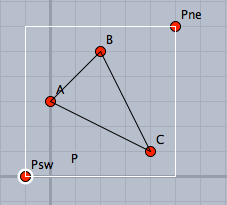
\includegraphics[bb=0 0 227 205 , width=4cm]{Fig/setorigin.png}  %%% test.tex 2014-11-28 22:0
%%% test.sce 2014-11-28 22:0
{\unitlength=6mm%
\begin{picture}%
(   6.00000,   6.00000)(  -1.00000,   0.00000)%
\special{pn 8}%
%
\special{pa 245 -245}\special{pa 238 -248}\special{pa 231 -247}\special{pa 226 -242}%
\special{pa 225 -234}\special{pa 228 -228}\special{pa 234 -225}\special{pa 242 -226}%
\special{pa 247 -231}\special{pa 248 -238}\special{pa 245 -245}\special{sh 1}\special{fp}%
\settowidth{\Width}{P}\setlength{\Width}{-0.5\Width}%
\settoheight{\Height}{P}\settodepth{\Depth}{P}\setlength{\Height}{-\Height}%
\put(1.0000,0.8500){\hspace*{\Width}\raisebox{\Height}{P}}%
%
%
\special{pa 0 -709}\special{pa 472 -1181}\special{pa 945 -236}\special{pa 0 -709}%
\special{fp}%
\special{pa -236 -472}\special{pa 1181 -472}%
\special{fp}%
\special{pa 709 0}\special{pa 709 -1417}%
\special{fp}%
\settowidth{\Width}{$x$}\setlength{\Width}{0\Width}%
\settoheight{\Height}{$x$}\settodepth{\Depth}{$x$}\setlength{\Height}{-0.5\Height}\setlength{\Depth}{0.5\Depth}\addtolength{\Height}{\Depth}%
\put(5.0500,2.0000){\hspace*{\Width}\raisebox{\Height}{$x$}}%
%
%
\settowidth{\Width}{$y$}\setlength{\Width}{-0.5\Width}%
\settoheight{\Height}{$y$}\settodepth{\Depth}{$y$}\setlength{\Height}{\Depth}%
\put(3.0000,6.0500){\hspace*{\Width}\raisebox{\Height}{$y$}}%
%
%
\settowidth{\Width}{O}\setlength{\Width}{-1\Width}%
\settoheight{\Height}{O}\settodepth{\Depth}{O}\setlength{\Height}{-\Height}%
\put(2.9500,1.9500){\hspace*{\Width}\raisebox{\Height}{O}}%
%
%
\end{picture}}%\\
 \\
\hypertarget{setpen}{}
\item[関数] Setpen(数)    
\item[機能] 線の太さを設定する\\
 \\[-5mm]
\begin{flushright} \hyperlink{functionlist}{$\Rightarrow$関数一覧}\end{flushright}
 \\
\hypertarget{setpt}{}
\item[関数] Setpt(数)       
\item[機能] 表示する点の大きさを設定する\\

\hypertarget{setscaling}{}
\item[関数] Setscaling(倍率)
\item[機能] 縦方向の倍率を設定する
\item[説明] 2次関数の応用問題などでは,グラフが縦に大きくなる場合があり,$y$軸方向のスケーリングを変えることがよくある。次のスクリプトは,$f(x)=-x^2+10x$ のグラフを縦軸方向を半分にして描くものである。\\
\begin{layer}{150}{0}
\putnotese{80}{0}{%%% test.tex 2014-10-22 10:38
%%% test.sce 2014-10-22 10:38
{\unitlength=5mm%
\begin{picture}%
(   7.00000,   8.00000)(  -1.00000,  -1.00000)%
\special{pn 8}%
%
\special{pn 8}%
\special{pa -4 -1230}\special{pa 4 -1230}\special{fp}\special{pa 34 -1230}\special{pa 42 -1230}\special{fp}%
\special{pa 72 -1230}\special{pa 80 -1230}\special{fp}\special{pa 110 -1230}\special{pa 118 -1230}\special{fp}%
\special{pa 147 -1230}\special{pa 155 -1230}\special{fp}\special{pa 185 -1230}\special{pa 193 -1230}\special{fp}%
\special{pa 223 -1230}\special{pa 231 -1230}\special{fp}\special{pa 261 -1230}\special{pa 269 -1230}\special{fp}%
\special{pa 299 -1230}\special{pa 307 -1230}\special{fp}\special{pa 337 -1230}\special{pa 345 -1230}\special{fp}%
\special{pa 375 -1230}\special{pa 383 -1230}\special{fp}\special{pa 412 -1230}\special{pa 420 -1230}\special{fp}%
\special{pa 450 -1230}\special{pa 458 -1230}\special{fp}\special{pa 488 -1230}\special{pa 496 -1230}\special{fp}%
\special{pn 8}%
\special{pn 8}%
\special{pa 492 4}\special{pa 492 -4}\special{fp}\special{pa 492 -36}\special{pa 492 -44}\special{fp}%
\special{pa 492 -75}\special{pa 492 -83}\special{fp}\special{pa 492 -115}\special{pa 492 -123}\special{fp}%
\special{pa 492 -155}\special{pa 492 -163}\special{fp}\special{pa 492 -194}\special{pa 492 -202}\special{fp}%
\special{pa 492 -234}\special{pa 492 -242}\special{fp}\special{pa 492 -274}\special{pa 492 -282}\special{fp}%
\special{pa 492 -314}\special{pa 492 -322}\special{fp}\special{pa 492 -353}\special{pa 492 -361}\special{fp}%
\special{pa 492 -393}\special{pa 492 -401}\special{fp}\special{pa 492 -433}\special{pa 492 -441}\special{fp}%
\special{pa 492 -472}\special{pa 492 -480}\special{fp}\special{pa 492 -512}\special{pa 492 -520}\special{fp}%
\special{pa 492 -552}\special{pa 492 -560}\special{fp}\special{pa 492 -591}\special{pa 492 -599}\special{fp}%
\special{pa 492 -631}\special{pa 492 -639}\special{fp}\special{pa 492 -671}\special{pa 492 -679}\special{fp}%
\special{pa 492 -710}\special{pa 492 -718}\special{fp}\special{pa 492 -750}\special{pa 492 -758}\special{fp}%
\special{pa 492 -790}\special{pa 492 -798}\special{fp}\special{pa 492 -829}\special{pa 492 -837}\special{fp}%
\special{pa 492 -869}\special{pa 492 -877}\special{fp}\special{pa 492 -909}\special{pa 492 -917}\special{fp}%
\special{pa 492 -949}\special{pa 492 -957}\special{fp}\special{pa 492 -988}\special{pa 492 -996}\special{fp}%
\special{pa 492 -1028}\special{pa 492 -1036}\special{fp}\special{pa 492 -1068}\special{pa 492 -1076}\special{fp}%
\special{pa 492 -1107}\special{pa 492 -1115}\special{fp}\special{pa 492 -1147}\special{pa 492 -1155}\special{fp}%
\special{pa 492 -1187}\special{pa 492 -1195}\special{fp}\special{pa 492 -1226}\special{pa 492 -1234}\special{fp}%
\special{pn 8}%
\settowidth{\Width}{5}\setlength{\Width}{-1\Width}%
\settoheight{\Height}{5}\settodepth{\Depth}{5}\setlength{\Height}{-\Height}%
\put(4.9500,-0.1500){\hspace*{\Width}\raisebox{\Height}{5}}%
%
%
\settowidth{\Width}{$\frac{25}{2}$}\setlength{\Width}{-1\Width}%
\settoheight{\Height}{$\frac{25}{2}$}\settodepth{\Depth}{$\frac{25}{2}$}\setlength{\Height}{-0.5\Height}\setlength{\Depth}{0.5\Depth}\addtolength{\Height}{\Depth}%
\put(-0.1500,6.2500){\hspace*{\Width}\raisebox{\Height}{$\frac{25}{2}$}}%
%
%
\settowidth{\Width}{$\frac{5}{2}$}\setlength{\Width}{-0.5\Width}%
\settoheight{\Height}{$\frac{5}{2}$}\settodepth{\Depth}{$\frac{5}{2}$}\setlength{\Height}{-\Height}%
\put(2.5000,-0.2500){\hspace*{\Width}\raisebox{\Height}{$\frac{5}{2}$}}%
%
%
\special{pa -38 197}\special{pa -28 145}\special{pa 0 0}\special{pa 28 -137}\special{pa 56 -265}%
\special{pa 84 -386}\special{pa 112 -498}\special{pa 141 -603}\special{pa 169 -699}%
\special{pa 197 -787}\special{pa 225 -868}\special{pa 253 -940}\special{pa 281 -1004}%
\special{pa 309 -1061}\special{pa 337 -1109}\special{pa 366 -1149}\special{pa 394 -1181}%
\special{pa 422 -1205}\special{pa 450 -1221}\special{pa 478 -1229}\special{pa 506 -1229}%
\special{pa 534 -1221}\special{pa 562 -1205}\special{pa 591 -1181}\special{pa 619 -1149}%
\special{pa 647 -1109}\special{pa 675 -1061}\special{pa 703 -1004}\special{pa 731 -940}%
\special{pa 759 -868}\special{pa 787 -787}\special{pa 816 -699}\special{pa 844 -603}%
\special{pa 872 -498}\special{pa 900 -386}\special{pa 928 -265}\special{pa 956 -137}%
\special{pa 984 0}\special{pa 1012 145}\special{pa 1022 197}%
\special{fp}%
\special{pa -197 0}\special{pa 1181 0}%
\special{fp}%
\special{pa 0 197}\special{pa 0 -1378}%
\special{fp}%
\settowidth{\Width}{$x$}\setlength{\Width}{0\Width}%
\settoheight{\Height}{$x$}\settodepth{\Depth}{$x$}\setlength{\Height}{-0.5\Height}\setlength{\Depth}{0.5\Depth}\addtolength{\Height}{\Depth}%
\put(6.0500,0.0000){\hspace*{\Width}\raisebox{\Height}{$x$}}%
%
%
\settowidth{\Width}{$y$}\setlength{\Width}{-0.5\Width}%
\settoheight{\Height}{$y$}\settodepth{\Depth}{$y$}\setlength{\Height}{\Depth}%
\put(0.0000,7.0500){\hspace*{\Width}\raisebox{\Height}{$y$}}%
%
%
\settowidth{\Width}{O}\setlength{\Width}{-1\Width}%
\settoheight{\Height}{O}\settodepth{\Depth}{O}\setlength{\Height}{-\Height}%
\put(-0.0500,-0.0500){\hspace*{\Width}\raisebox{\Height}{O}}%
%
%
\end{picture}}%}
\end{layer}
 \\
\begin{verbatim}
 Setscaling(0.5);
 A.xy=[0,25/4];
 B.xy=[5/2,25/4];
 C.xy=[5/2,0];
 Listplot([A,B],["do"]);
 Listplot([C,B],["do"]);
 Plotdata("1","-2*x^2+10*x","x");
 Letter([[5,0],"s2w","5",[0,25/2],"w2",
    "$\frac{25}{2}$",C,"s4","$\frac{5}{2}$"]);
\end{verbatim}
%          %%% test.tex 2014-10-22 10:38
%%% test.sce 2014-10-22 10:38
{\unitlength=5mm%
\begin{picture}%
(   7.00000,   8.00000)(  -1.00000,  -1.00000)%
\special{pn 8}%
%
\special{pn 8}%
\special{pa -4 -1230}\special{pa 4 -1230}\special{fp}\special{pa 34 -1230}\special{pa 42 -1230}\special{fp}%
\special{pa 72 -1230}\special{pa 80 -1230}\special{fp}\special{pa 110 -1230}\special{pa 118 -1230}\special{fp}%
\special{pa 147 -1230}\special{pa 155 -1230}\special{fp}\special{pa 185 -1230}\special{pa 193 -1230}\special{fp}%
\special{pa 223 -1230}\special{pa 231 -1230}\special{fp}\special{pa 261 -1230}\special{pa 269 -1230}\special{fp}%
\special{pa 299 -1230}\special{pa 307 -1230}\special{fp}\special{pa 337 -1230}\special{pa 345 -1230}\special{fp}%
\special{pa 375 -1230}\special{pa 383 -1230}\special{fp}\special{pa 412 -1230}\special{pa 420 -1230}\special{fp}%
\special{pa 450 -1230}\special{pa 458 -1230}\special{fp}\special{pa 488 -1230}\special{pa 496 -1230}\special{fp}%
\special{pn 8}%
\special{pn 8}%
\special{pa 492 4}\special{pa 492 -4}\special{fp}\special{pa 492 -36}\special{pa 492 -44}\special{fp}%
\special{pa 492 -75}\special{pa 492 -83}\special{fp}\special{pa 492 -115}\special{pa 492 -123}\special{fp}%
\special{pa 492 -155}\special{pa 492 -163}\special{fp}\special{pa 492 -194}\special{pa 492 -202}\special{fp}%
\special{pa 492 -234}\special{pa 492 -242}\special{fp}\special{pa 492 -274}\special{pa 492 -282}\special{fp}%
\special{pa 492 -314}\special{pa 492 -322}\special{fp}\special{pa 492 -353}\special{pa 492 -361}\special{fp}%
\special{pa 492 -393}\special{pa 492 -401}\special{fp}\special{pa 492 -433}\special{pa 492 -441}\special{fp}%
\special{pa 492 -472}\special{pa 492 -480}\special{fp}\special{pa 492 -512}\special{pa 492 -520}\special{fp}%
\special{pa 492 -552}\special{pa 492 -560}\special{fp}\special{pa 492 -591}\special{pa 492 -599}\special{fp}%
\special{pa 492 -631}\special{pa 492 -639}\special{fp}\special{pa 492 -671}\special{pa 492 -679}\special{fp}%
\special{pa 492 -710}\special{pa 492 -718}\special{fp}\special{pa 492 -750}\special{pa 492 -758}\special{fp}%
\special{pa 492 -790}\special{pa 492 -798}\special{fp}\special{pa 492 -829}\special{pa 492 -837}\special{fp}%
\special{pa 492 -869}\special{pa 492 -877}\special{fp}\special{pa 492 -909}\special{pa 492 -917}\special{fp}%
\special{pa 492 -949}\special{pa 492 -957}\special{fp}\special{pa 492 -988}\special{pa 492 -996}\special{fp}%
\special{pa 492 -1028}\special{pa 492 -1036}\special{fp}\special{pa 492 -1068}\special{pa 492 -1076}\special{fp}%
\special{pa 492 -1107}\special{pa 492 -1115}\special{fp}\special{pa 492 -1147}\special{pa 492 -1155}\special{fp}%
\special{pa 492 -1187}\special{pa 492 -1195}\special{fp}\special{pa 492 -1226}\special{pa 492 -1234}\special{fp}%
\special{pn 8}%
\settowidth{\Width}{5}\setlength{\Width}{-1\Width}%
\settoheight{\Height}{5}\settodepth{\Depth}{5}\setlength{\Height}{-\Height}%
\put(4.9500,-0.1500){\hspace*{\Width}\raisebox{\Height}{5}}%
%
%
\settowidth{\Width}{$\frac{25}{2}$}\setlength{\Width}{-1\Width}%
\settoheight{\Height}{$\frac{25}{2}$}\settodepth{\Depth}{$\frac{25}{2}$}\setlength{\Height}{-0.5\Height}\setlength{\Depth}{0.5\Depth}\addtolength{\Height}{\Depth}%
\put(-0.1500,6.2500){\hspace*{\Width}\raisebox{\Height}{$\frac{25}{2}$}}%
%
%
\settowidth{\Width}{$\frac{5}{2}$}\setlength{\Width}{-0.5\Width}%
\settoheight{\Height}{$\frac{5}{2}$}\settodepth{\Depth}{$\frac{5}{2}$}\setlength{\Height}{-\Height}%
\put(2.5000,-0.2500){\hspace*{\Width}\raisebox{\Height}{$\frac{5}{2}$}}%
%
%
\special{pa -38 197}\special{pa -28 145}\special{pa 0 0}\special{pa 28 -137}\special{pa 56 -265}%
\special{pa 84 -386}\special{pa 112 -498}\special{pa 141 -603}\special{pa 169 -699}%
\special{pa 197 -787}\special{pa 225 -868}\special{pa 253 -940}\special{pa 281 -1004}%
\special{pa 309 -1061}\special{pa 337 -1109}\special{pa 366 -1149}\special{pa 394 -1181}%
\special{pa 422 -1205}\special{pa 450 -1221}\special{pa 478 -1229}\special{pa 506 -1229}%
\special{pa 534 -1221}\special{pa 562 -1205}\special{pa 591 -1181}\special{pa 619 -1149}%
\special{pa 647 -1109}\special{pa 675 -1061}\special{pa 703 -1004}\special{pa 731 -940}%
\special{pa 759 -868}\special{pa 787 -787}\special{pa 816 -699}\special{pa 844 -603}%
\special{pa 872 -498}\special{pa 900 -386}\special{pa 928 -265}\special{pa 956 -137}%
\special{pa 984 0}\special{pa 1012 145}\special{pa 1022 197}%
\special{fp}%
\special{pa -197 0}\special{pa 1181 0}%
\special{fp}%
\special{pa 0 197}\special{pa 0 -1378}%
\special{fp}%
\settowidth{\Width}{$x$}\setlength{\Width}{0\Width}%
\settoheight{\Height}{$x$}\settodepth{\Depth}{$x$}\setlength{\Height}{-0.5\Height}\setlength{\Depth}{0.5\Depth}\addtolength{\Height}{\Depth}%
\put(6.0500,0.0000){\hspace*{\Width}\raisebox{\Height}{$x$}}%
%
%
\settowidth{\Width}{$y$}\setlength{\Width}{-0.5\Width}%
\settoheight{\Height}{$y$}\settodepth{\Depth}{$y$}\setlength{\Height}{\Depth}%
\put(0.0000,7.0500){\hspace*{\Width}\raisebox{\Height}{$y$}}%
%
%
\settowidth{\Width}{O}\setlength{\Width}{-1\Width}%
\settoheight{\Height}{O}\settodepth{\Depth}{O}\setlength{\Height}{-\Height}%
\put(-0.0500,-0.0500){\hspace*{\Width}\raisebox{\Height}{O}}%
%
%
\end{picture}}%\\
 ここで,点A,Bの座標が
\begin{verbatim}
  A.xy=[0,25/4];
  B.xy=[5/2,25/4];
\end{verbatim}
となっていることに注意されたい。$y$座標をあらかじめ半分にしている。すなわち,Cinderellaで作図した幾何要素に対してはSetscalingは無効である。これは,Putpoint関数を用いて点の位置を決めても同じである。\\
 たとえば,次のスクリプトでは,Cinderellaの画面上では2本の線分が点Bでつながるが,書き出された\TeX の図では離れてしまう。
\begin{verbatim}
  Setscaling(0.5);
  Putpoint("A",[0,2]);
  Putpoint("B",[2,2]);
  Listplot([A,B]);
  Listplot("1",[[0,0],[2,2]]);
\end{verbatim}
 \\
 \\
%\newpage
\hypertarget{setunitlen}{}
\item[関数] Setunitlen(文字列)
\item[機能] 単位長を設定する。デフォルトは 1cm\\
 \\
 \\
\hypertarget{setwindow}{}
\item[関数] Setwindow()
\item[機能] 出力する描画領域を設定する\\
\item[説明] 出力する描画領域は,通常は2点SWとNEを対角とする矩形領域である。
この2点をドラッグすることによりビジュアルに描画領域を決められる。\\
しかし,これとは別に出力範囲を設定したい場合にこの関数を用いる。\\
また,表を作成したときは,表の範囲が出力範囲として優先される(Tabledata()を実行したとき)ので,表外に図を描いた場合は,最後にこの関数で出力範囲を指定して書き出す。\\
 \\
\end{description}

\begin{flushright} \hyperlink{functionlist}{$\Rightarrow$関数一覧}\end{flushright}
\newpage
%第5節=================================
\subsection{描画}

描画関数は曲線などを作図する関数である。\\
 基本的な書式は\\
   関数名(name , 点リストなど , options);\\
であるが,nameの不要なものもある。\\
 nameは,プロットデータの名称を指定するもので,関数ごとに決められた頭部のあとに付けられる。nameが不要の場合は \ketcindy が自動的に名称を作成する。\\
 点リストなどは,点の座標,点の識別名,複数の点のリスト,複数の点を示す文字列などがあり,関数によって異なる。点はCinderellaで作図した幾何要素の点を利用できる。\\
 \\
 optionsは,線種・表示する文字列・解像度・出力の有無などを指定するオプション群。
\begin{tabbing}
1234567890123\=\kill
 線種はつぎの4通り。デフォルトは実線。\\
  "dr, n"   \>太さnの実線で描く。Scilab のファイルに Drwline() を出力する。\\
  "da,m,n" \>破線を描く。Scilab のファイルに Dashline() を出力する。\\
        \> mは破線の長さ,nは破線の間隔 (m,nは省略可)\\
        \>m,n オプションはCinderellaの描画面には反映されない。\\
  "id,m,n" \>ギャップからはじまる破線を描く。Scilab のファイルに Invdashline() を出力する。\\
  "do,m,n" \>点線で描く。Scilab のファイルに Dottedline() を出力する。\\
        \>mは点の間隔,nは太さ (m,nは省略可)\\
 描画色指定は,Cindyscriptの表記と同様で,RGBのリストで指定するか,色名を用いる。\\
  例:\verb|"color->[0,0.7,0]"| で暗い緑になる。\\
 出力の有無は\\
  "notex" \>Cinderella画面上で補助線として用いた図形をScilabに出力しない\\
  "nodisp" \>Cinderella画面上にも出力しない\\

   "nodisp"は画面上にも,Scilabへのデータにも出力されないが,プロットデータは作成され,\\
   それを戻り値とするので,プロットデータだけを利用したい場合に有効である。\\
   例 \verb|pdata=Circledata([A,B],["nodisp"]);|\\
    として,プロットデータ pdata を処理する。\\
\end{tabbing}

\newpage
\begin{description}

\hypertarget{anglemark}{}
\item[関数] Anglemark(点リスト , options)
\item[機能] 点リスト[A,B,C]で示された角に弧の形状の角の印をつける。
\item[説明] optionsは次の通り。\\
  数値   角の印の大きさ。デフォルトは1\\
  線種   "dr, n"  , "da,m,n" , "do,m,n"\\
  "Expr=文字"  : 文字を入れる\\
  "Expr=位置 , 文字"  : 位置を指定して文字を入れる。位置は頂点からの距離。\\

例:三角形の内角に印をいれ,文字を書き込む。
\begin{verbatim}
   Listplot([A,B,C,A]);
   Letter([A,"n1","A",B,"w1","B",C,"e1","C"]);
   Anglemark([B,A,C]);
   Anglemark([C,B,A],["Expr=\theta"]);
   Anglemark([A,C,B],[2,"dr,3","Expr=2,\alpha"]);
\end{verbatim}
 %%% anglemark.tex 2014-11-10 8:47
%%% anglemark.sce 2014-11-10 8:36
{\unitlength=1cm%
\begin{picture}%
(   6.00000,   5.00000)(  -3.00000,  -2.00000)%
\special{pn 8}%
%
\settowidth{\Width}{A}\setlength{\Width}{-0.5\Width}%
\settoheight{\Height}{A}\settodepth{\Depth}{A}\setlength{\Height}{\Depth}%
\put(-0.4600,2.1100){\hspace*{\Width}\raisebox{\Height}{A}}%
%
%
\settowidth{\Width}{B}\setlength{\Width}{-1\Width}%
\settoheight{\Height}{B}\settodepth{\Depth}{B}\setlength{\Height}{-0.5\Height}\setlength{\Depth}{0.5\Depth}\addtolength{\Height}{\Depth}%
\put(-2.1000,-1.0000){\hspace*{\Width}\raisebox{\Height}{B}}%
%
%
\settowidth{\Width}{C}\setlength{\Width}{0\Width}%
\settoheight{\Height}{C}\settodepth{\Depth}{C}\setlength{\Height}{-0.5\Height}\setlength{\Depth}{0.5\Depth}\addtolength{\Height}{\Depth}%
\put(2.1000,-1.0000){\hspace*{\Width}\raisebox{\Height}{C}}%
%
%
\settowidth{\Width}{$\theta$}\setlength{\Width}{-0.5\Width}%
\settoheight{\Height}{$\theta$}\settodepth{\Depth}{$\theta$}\setlength{\Height}{-0.5\Height}\setlength{\Depth}{0.5\Depth}\addtolength{\Height}{\Depth}%
\put(-1.3600,-0.6100){\hspace*{\Width}\raisebox{\Height}{$\theta$}}%
%
%
\settowidth{\Width}{$\alpha$}\setlength{\Width}{-0.5\Width}%
\settoheight{\Height}{$\alpha$}\settodepth{\Depth}{$\alpha$}\setlength{\Height}{-0.5\Height}\setlength{\Depth}{0.5\Depth}\addtolength{\Height}{\Depth}%
\put(0.1900,-0.1400){\hspace*{\Width}\raisebox{\Height}{$\alpha$}}%
%
%
\special{pn 24}%
\special{pa 538 89}\special{pa 536 90}\special{pa 500 124}\special{pa 469 162}\special{pa 442 204}%
\special{pa 421 249}\special{pa 406 296}\special{pa 397 344}\special{pa 394 394}%
\special{fp}%
\special{pn 8}%
\special{pa -181 -791}\special{pa -787 394}\special{pa 787 394}\special{pa -181 -791}%
\special{fp}%
\special{pa -271 -616}\special{pa -265 -613}\special{pa -242 -604}\special{pa -218 -598}%
\special{pa -193 -595}\special{pa -169 -595}\special{pa -144 -598}\special{pa -120 -604}%
\special{pa -97 -613}\special{pa -76 -625}\special{pa -57 -639}%
\special{fp}%
\special{pa -591 394}\special{pa -592 369}\special{pa -597 345}\special{pa -604 321}%
\special{pa -615 299}\special{pa -628 278}\special{pa -644 259}\special{pa -662 242}%
\special{pa -682 227}\special{pa -698 219}%
\special{fp}%
\end{picture}}%

※角の印には平行四辺形の形状のものもある。Paramark() を参照のこと。\\

\begin{flushright} \hyperlink{functionlist}{$\Rightarrow$関数一覧}\end{flushright}

\hypertarget{arrowdata}{}
\item[関数] Arrowdata(name,[始点 , 終点] , options) 
\item[機能] 2点間を結ぶ矢線を描く。プロットデータ名の頭部は ar
\item[説明] name は,座標を数値で与えるときに必要。幾何要素の識別名で与えるときはなくてもよい。\\
 optionsは矢じりの形状などの指定で\\
  [ 矢じりの大きさ, 開き角, 矢じり位置, 線種,線の表示色] 
 のリストで与える。\\
 開き角は60分法で与える。ただし,° はつけない。5未満の時は18°の倍数指定とする。\\
 矢じり位置は,線分の長さを1とした始点からの距離。\\
 ただし,Cinderellaの画面上には全ては反映されない。たとえば,太さ指定をしても太さは同じ。\\

 例:線分ABを矢線にする。\\
    \verb|Arrowdata([A,B]);|\\
   始点が(2,0) , 終点が(4,3) ,開き角45°,EFの中点に矢じりの先端\\
    \verb|Arrowdata("1",[[2,0],[4,3]],[1,45,0.5]);|\\
   大きさ2,太さ2\\
    \verb|Arrowdata([C,D],[2,1,1,"dr,2"]);|\\
   破線で太さ0.5\\
    \verb|Arrowdata([E,F],["da,0.5"]);|\\
   少し間が空いて太い点線で,Cinderellaの画面上では赤で表示する。\\
    \verb|Arrowdata([G,H],[2,1,"do,2,3","color-$>$[1,0,0]"]);| \\

   %%% test.tex 2014-11-30 20:20
%%% test.sce 2014-11-30 20:20
{\unitlength=6mm%
\begin{picture}%
(  12.56000,   5.04000)(  -1.00000,  -1.00000)%
\special{pn 8}%
%
\special{pa 451 -633}\special{pa 472 -709}\special{pa 411 -660}\special{pa 431 -646}%
\special{pa 451 -633}\special{sh 1}\special{ip}%
\special{pn 8}%
\special{pa 451 -633}\special{pa 472 -709}\special{pa 411 -660}\special{pa 431 -646}%
\special{pa 451 -633}%
\special{fp}%
\special{pn 8}%
\special{pa 724 -277}\special{pa 709 -354}\special{pa 631 -339}\special{pa 678 -308}%
\special{pa 724 -277}\special{sh 1}\special{ip}%
\special{pn 8}%
\special{pa 724 -277}\special{pa 709 -354}\special{pa 631 -339}\special{pa 678 -308}%
\special{pa 724 -277}%
\special{fp}%
\special{pn 8}%
\special{pn 16}%
\special{pa 945 0}\special{pa 1417 -709}%
\special{fp}%
\special{pn 8}%
\special{pa 1375 -557}\special{pa 1417 -709}\special{pa 1294 -611}\special{pa 1334 -584}%
\special{pa 1375 -557}\special{sh 1}\special{ip}%
\special{pn 8}%
\special{pa 1375 -557}\special{pa 1417 -709}\special{pa 1294 -611}\special{pa 1334 -584}%
\special{pa 1375 -557}%
\special{fp}%
\special{pn 8}%
\special{pa 1417 0}\special{pa 1428 -16}\special{fp}\special{pa 1438 -31}\special{pa 1449 -47}\special{fp}%
\special{pa 1459 -63}\special{pa 1470 -79}\special{fp}\special{pa 1480 -94}\special{pa 1491 -110}\special{fp}%
\special{pa 1501 -126}\special{pa 1512 -142}\special{fp}\special{pa 1522 -157}\special{pa 1533 -173}\special{fp}%
\special{pa 1543 -189}\special{pa 1554 -205}\special{fp}\special{pa 1564 -220}\special{pa 1575 -236}\special{fp}%
\special{pa 1585 -252}\special{pa 1596 -268}\special{fp}\special{pa 1606 -283}\special{pa 1617 -299}\special{fp}%
\special{pa 1627 -315}\special{pa 1638 -331}\special{fp}\special{pa 1648 -346}\special{pa 1659 -362}\special{fp}%
\special{pa 1669 -378}\special{pa 1680 -394}\special{fp}\special{pa 1690 -409}\special{pa 1701 -425}\special{fp}%
\special{pa 1711 -441}\special{pa 1722 -457}\special{fp}\special{pa 1732 -472}\special{pa 1743 -488}\special{fp}%
\special{pa 1753 -504}\special{pa 1764 -520}\special{fp}\special{pa 1774 -535}\special{pa 1785 -551}\special{fp}%
\special{pa 1795 -567}\special{pa 1806 -583}\special{fp}\special{pa 1816 -598}\special{pa 1827 -614}\special{fp}%
\special{pa 1837 -630}\special{pa 1848 -646}\special{fp}\special{pa 1858 -661}\special{pa 1869 -677}\special{fp}%
\special{pa 1879 -693}\special{pa 1890 -709}\special{fp}%
%
\special{pa 1868 -633}\special{pa 1890 -709}\special{pa 1828 -660}\special{pa 1848 -646}%
\special{pa 1868 -633}\special{sh 1}\special{ip}%
\special{pn 8}%
\special{pa 1868 -633}\special{pa 1890 -709}\special{pa 1828 -660}\special{pa 1848 -646}%
\special{pa 1868 -633}%
\special{fp}%
\special{pn 8}%
\special{pn 24}%
\special{pa 1883 10}\special{pa 1896 -10}\special{fp}\special{pa 1926 -54}\special{pa 1939 -74}\special{fp}%
\special{pa 1969 -119}\special{pa 1982 -139}\special{fp}\special{pa 2012 -183}\special{pa 2025 -203}\special{fp}%
\special{pa 2055 -248}\special{pa 2068 -268}\special{fp}\special{pa 2098 -312}\special{pa 2111 -332}\special{fp}%
\special{pa 2141 -377}\special{pa 2154 -397}\special{fp}\special{pa 2184 -441}\special{pa 2197 -461}\special{fp}%
\special{pa 2227 -505}\special{pa 2240 -525}\special{fp}\special{pa 2270 -570}\special{pa 2283 -590}\special{fp}%
\special{pa 2313 -634}\special{pa 2326 -654}\special{fp}\special{pa 2356 -699}\special{pa 2369 -719}\special{fp}%
\special{pn 8}%
\special{pa 2320 -557}\special{pa 2362 -709}\special{pa 2239 -611}\special{pa 2279 -584}%
\special{pa 2320 -557}\special{sh 1}\special{ip}%
\special{pn 8}%
\special{pa 2320 -557}\special{pa 2362 -709}\special{pa 2239 -611}\special{pa 2279 -584}%
\special{pa 2320 -557}%
\special{fp}%
\special{pn 8}%
\special{pa 0 0}\special{pa 472 -709}%
\special{fp}%
\special{pa 472 0}\special{pa 945 -709}%
\special{fp}%
\end{picture}}%\\
\\

\begin{flushright} \hyperlink{functionlist}{$\Rightarrow$関数一覧}\end{flushright}

\hypertarget{arrowhead}{}
\item[関数] Arrowhead(点 , 方向 , options) , Arrowhead(点 , プロットデータ,options)
\item[機能] 点に矢じりだけを描く
\item[説明] 指定された位置に,指定された方向を向いた矢じりだけを描く。\\
 点は座標または幾何要素名。方向は原点から見て座標[a,b]の方向。\\
 optionsは [大きさ,矢じりの開き角,形状と位置] のリスト。\\
 矢じりの開き角は60分法で片側半分の角。\\
 形状は, "f" :塗りつぶしの三角形(デフォルト)または " l " : ラインのみ。\\ 
 位置は,"t"(デフォルト)または "c" , "b"\\
   "t" は矢じりの先端が終点に一致,"c" は三角形の中心が終点と一致,"b" は終点が矢じりの底辺にのる。\\
 プロットデータを指定したときは,曲線上の点に矢じりをつける。\\
 曲線には向きがあり,それによって矢じりの向きが決まる。" Invert(プロットデータ) " とすると反対向きの矢じりになる。\\
 曲線の向きとは,曲線を描くときの順序で,プロットデータの順序でもある。invert() はこのプロットデータを逆順にするものである。\\

例:

\vspace{-8mm}
\hspace{6mm}
\begin{layer}{150}{0}
\putnotese{0}{0}{点 A が下図の位置のとき}
\putnotese{0}{8}{%%% ForRef-Arrowhead-1.tex 2014-11-10 7:14
%%% ForRef-Arrowhead5all.sce~ 2014-11-10 6:59
{\unitlength=1cm%
\begin{picture}%
(   2.03000,   2.02000)(  -0.56000,  -0.53000)%
\special{pn 8}%
%
\special{pn 8}%
\special{pa 394 4}\special{pa 394 -4}\special{fp}\special{pa 394 -35}\special{pa 394 -43}\special{fp}%
\special{pa 394 -75}\special{pa 394 -83}\special{fp}\special{pa 394 -114}\special{pa 394 -122}\special{fp}%
\special{pa 394 -153}\special{pa 394 -161}\special{fp}\special{pa 394 -193}\special{pa 394 -201}\special{fp}%
\special{pa 394 -232}\special{pa 394 -240}\special{fp}\special{pa 394 -272}\special{pa 394 -280}\special{fp}%
\special{pa 394 -311}\special{pa 394 -319}\special{fp}\special{pa 394 -350}\special{pa 394 -358}\special{fp}%
\special{pa 397 -391}\special{pa 391 -397}\special{fp}\special{pa 358 -394}\special{pa 350 -394}\special{fp}%
\special{pa 319 -394}\special{pa 311 -394}\special{fp}\special{pa 280 -394}\special{pa 272 -394}\special{fp}%
\special{pa 240 -394}\special{pa 232 -394}\special{fp}\special{pa 201 -394}\special{pa 193 -394}\special{fp}%
\special{pa 161 -394}\special{pa 153 -394}\special{fp}\special{pa 122 -394}\special{pa 114 -394}\special{fp}%
\special{pa 83 -394}\special{pa 75 -394}\special{fp}\special{pa 43 -394}\special{pa 35 -394}\special{fp}%
\special{pa 4 -394}\special{pa -4 -394}\special{fp}\special{pn 8}%
\special{pa 408 -408}\special{pa 400 -412}\special{pa 390 -413}\special{pa 382 -409}%
\special{pa 376 -402}\special{pa 374 -393}\special{pa 377 -384}\special{pa 384 -377}%
\special{pa 393 -374}\special{pa 402 -376}\special{pa 409 -382}\special{pa 413 -390}%
\special{pa 412 -400}\special{pa 408 -408}\special{sh 1}\special{fp}%
\settowidth{\Width}{A}\setlength{\Width}{0\Width}%
\settoheight{\Height}{A}\settodepth{\Depth}{A}\setlength{\Height}{\Depth}%
\put(1.1000,1.1000){\hspace*{\Width}\raisebox{\Height}{A}}%
%
%
\special{pa 394 -20}\special{pa 394 20}%
\special{fp}%
\settowidth{\Width}{$1$}\setlength{\Width}{-0.5\Width}%
\settoheight{\Height}{$1$}\settodepth{\Depth}{$1$}\setlength{\Height}{-\Height}%
\put(1.0000,-0.1000){\hspace*{\Width}\raisebox{\Height}{$1$}}%
%
%
%
\special{pa 20 -394}\special{pa -20 -394}%
\special{fp}%
\settowidth{\Width}{$1$}\setlength{\Width}{-1\Width}%
\settoheight{\Height}{$1$}\settodepth{\Depth}{$1$}\setlength{\Height}{-0.5\Height}\setlength{\Depth}{0.5\Depth}\addtolength{\Height}{\Depth}%
\put(-0.1000,1.0000){\hspace*{\Width}\raisebox{\Height}{$1$}}%
%
%
%
\special{pa -220 0}\special{pa 579 0}%
\special{fp}%
\special{pa 0 209}\special{pa 0 -587}%
\special{fp}%
\settowidth{\Width}{$x$}\setlength{\Width}{0\Width}%
\settoheight{\Height}{$x$}\settodepth{\Depth}{$x$}\setlength{\Height}{-0.5\Height}\setlength{\Depth}{0.5\Depth}\addtolength{\Height}{\Depth}%
\put(1.5200,0.0000){\hspace*{\Width}\raisebox{\Height}{$x$}}%
%
%
\settowidth{\Width}{$y$}\setlength{\Width}{-0.5\Width}%
\settoheight{\Height}{$y$}\settodepth{\Depth}{$y$}\setlength{\Height}{\Depth}%
\put(0.0000,1.5400){\hspace*{\Width}\raisebox{\Height}{$y$}}%
%
%
\settowidth{\Width}{O}\setlength{\Width}{-1\Width}%
\settoheight{\Height}{O}\settodepth{\Depth}{O}\setlength{\Height}{-\Height}%
\put(-0.0500,-0.0500){\hspace*{\Width}\raisebox{\Height}{O}}%
%
%
\end{picture}}%}
\putnotese{40}{0}{(ア) Arrowhead(A,[-1,1]);}
\putnotese{40}{7}{(イ) Arrowhead([1,1],[-1,1],[2,60]);}
\putnotese{40}{14}{(ウ) Arrowhead(A,[-1,1],[2,30,"b"]);}
\putnotese{40}{21}{(エ) Arrowhead([1,1],[-1,1],[2,20,"lc"]);}
\end{layer}

\vspace{2mm}
\hspace{6mm}
\begin{layer}{150}{0}
\putnotese{0}{0}{%%% spline1.tex 2014-11-9 6:32
%%% spline1.sce 2014-11-8 22:24
{\unitlength=1cm%
\begin{picture}%
(  15.60000,  12.54000)(  -0.03000, -12.57000)%
\special{pn 8}%
%
\special{pn 0}%
\special{pa 3972 2358}\special{pa 3693 2220}\special{pa 3366 2189}\special{pa 3075 2228}%
\special{pa 2839 2339}%
\special{fp}%
\special{pn 8}%
\special{pa 3695 2190}\special{pa 3673 2171}\special{pa 3650 2153}\special{pa 3625 2137}%
\special{pa 3600 2123}\special{pa 3573 2109}\special{pa 3545 2097}\special{pa 3517 2086}%
\special{pa 3488 2076}\special{pa 3458 2068}\special{pa 3428 2060}\special{pa 3397 2053}%
\special{pa 3366 2048}\special{pa 3334 2043}\special{pa 3303 2039}\special{pa 3271 2036}%
\special{pa 3240 2034}\special{pa 3208 2033}\special{pa 3177 2032}\special{pa 3147 2032}%
\special{pa 3116 2033}\special{pa 3086 2034}\special{pa 3057 2036}\special{pa 3028 2039}%
\special{pa 3000 2042}\special{pa 2972 2045}\special{pa 2945 2050}\special{pa 2918 2055}%
\special{pa 2892 2061}\special{pa 2867 2067}\special{pa 2842 2074}\special{pa 2817 2082}%
\special{pa 2793 2091}\special{pa 2769 2100}\special{pa 2747 2110}\special{pa 2724 2121}%
\special{pa 2702 2132}\special{pa 2681 2145}\special{pa 2661 2158}\special{pa 2641 2171}%
\special{fp}%
\special{pn 8}%
\special{pa 2691 2111}\special{pa 2641 2171}\special{pa 2717 2152}\special{pa 2704 2132}%
\special{pa 2691 2111}\special{sh 1}\special{ip}%
\special{pn 8}%
\special{pa 2691 2111}\special{pa 2641 2171}\special{pa 2717 2152}\special{pa 2704 2132}%
\special{pa 2691 2111}%
\special{fp}%
\special{pn 8}%
\end{picture}}%}
\putnotese{95}{55}{D の座標がわかれ}
\putnotese{95}{60}{ば,それでもよい}
\putnotese{12}{27}{(ア)}
\putnotese{42}{27}{(イ)}
\putnotese{72}{27}{(ウ)}
\putnotese{102}{27}{(エ)}
\putnotese{0}{30}{%%% ForRef-Arrowhead-2.tex 2014-11-10 7:14
%%% ForRef-Arrowhead5all.sce~ 2014-11-10 6:59
{\unitlength=1cm%
\begin{picture}%
(   2.03000,   2.02000)(  -0.56000,  -0.53000)%
\special{pn 8}%
%
\special{pn 8}%
\special{pa 394 4}\special{pa 394 -4}\special{fp}\special{pa 394 -35}\special{pa 394 -43}\special{fp}%
\special{pa 394 -75}\special{pa 394 -83}\special{fp}\special{pa 394 -114}\special{pa 394 -122}\special{fp}%
\special{pa 394 -153}\special{pa 394 -161}\special{fp}\special{pa 394 -193}\special{pa 394 -201}\special{fp}%
\special{pa 394 -232}\special{pa 394 -240}\special{fp}\special{pa 394 -272}\special{pa 394 -280}\special{fp}%
\special{pa 394 -311}\special{pa 394 -319}\special{fp}\special{pa 394 -350}\special{pa 394 -358}\special{fp}%
\special{pa 397 -391}\special{pa 391 -397}\special{fp}\special{pa 358 -394}\special{pa 350 -394}\special{fp}%
\special{pa 319 -394}\special{pa 311 -394}\special{fp}\special{pa 280 -394}\special{pa 272 -394}\special{fp}%
\special{pa 240 -394}\special{pa 232 -394}\special{fp}\special{pa 201 -394}\special{pa 193 -394}\special{fp}%
\special{pa 161 -394}\special{pa 153 -394}\special{fp}\special{pa 122 -394}\special{pa 114 -394}\special{fp}%
\special{pa 83 -394}\special{pa 75 -394}\special{fp}\special{pa 43 -394}\special{pa 35 -394}\special{fp}%
\special{pa 4 -394}\special{pa -4 -394}\special{fp}\special{pn 8}%
\special{pa 464 -358}\special{pa 394 -394}\special{pa 429 -324}\special{pa 447 -341}%
\special{pa 464 -358}\special{sh 1}\special{ip}%
\special{pn 8}%
\special{pa 464 -358}\special{pa 394 -394}\special{pa 429 -324}\special{pa 447 -341}%
\special{pa 464 -358}%
\special{fp}%
\special{pn 8}%
\special{pa -220 0}\special{pa 579 0}%
\special{fp}%
\special{pa 0 209}\special{pa 0 -587}%
\special{fp}%
\settowidth{\Width}{$x$}\setlength{\Width}{0\Width}%
\settoheight{\Height}{$x$}\settodepth{\Depth}{$x$}\setlength{\Height}{-0.5\Height}\setlength{\Depth}{0.5\Depth}\addtolength{\Height}{\Depth}%
\put(1.5200,0.0000){\hspace*{\Width}\raisebox{\Height}{$x$}}%
%
%
\settowidth{\Width}{$y$}\setlength{\Width}{-0.5\Width}%
\settoheight{\Height}{$y$}\settodepth{\Depth}{$y$}\setlength{\Height}{\Depth}%
\put(0.0000,1.5400){\hspace*{\Width}\raisebox{\Height}{$y$}}%
%
%
\settowidth{\Width}{O}\setlength{\Width}{-1\Width}%
\settoheight{\Height}{O}\settodepth{\Depth}{O}\setlength{\Height}{-\Height}%
\put(-0.0500,-0.0500){\hspace*{\Width}\raisebox{\Height}{O}}%
%
%
\end{picture}}%}
\putnotese{30}{30}{%%% ForRef-Arrowhead-3.tex 2014-11-10 7:14
%%% ForRef-Arrowhead5all.sce~ 2014-11-10 6:59
{\unitlength=1cm%
\begin{picture}%
(   2.03000,   2.02000)(  -0.56000,  -0.53000)%
\special{pn 8}%
%
\special{pn 8}%
\special{pa 394 4}\special{pa 394 -4}\special{fp}\special{pa 394 -35}\special{pa 394 -43}\special{fp}%
\special{pa 394 -75}\special{pa 394 -83}\special{fp}\special{pa 394 -114}\special{pa 394 -122}\special{fp}%
\special{pa 394 -153}\special{pa 394 -161}\special{fp}\special{pa 394 -193}\special{pa 394 -201}\special{fp}%
\special{pa 394 -232}\special{pa 394 -240}\special{fp}\special{pa 394 -272}\special{pa 394 -280}\special{fp}%
\special{pa 394 -311}\special{pa 394 -319}\special{fp}\special{pa 394 -350}\special{pa 394 -358}\special{fp}%
\special{pa 397 -391}\special{pa 391 -397}\special{fp}\special{pa 358 -394}\special{pa 350 -394}\special{fp}%
\special{pa 319 -394}\special{pa 311 -394}\special{fp}\special{pa 280 -394}\special{pa 272 -394}\special{fp}%
\special{pa 240 -394}\special{pa 232 -394}\special{fp}\special{pa 201 -394}\special{pa 193 -394}\special{fp}%
\special{pa 161 -394}\special{pa 153 -394}\special{fp}\special{pa 122 -394}\special{pa 114 -394}\special{fp}%
\special{pa 83 -394}\special{pa 75 -394}\special{fp}\special{pa 43 -394}\special{pa 35 -394}\special{fp}%
\special{pa 4 -394}\special{pa -4 -394}\special{fp}\special{pn 8}%
\special{pa 546 -434}\special{pa 394 -394}\special{pa 353 -242}\special{pa 449 -338}%
\special{pa 546 -434}\special{sh 1}\special{ip}%
\special{pn 8}%
\special{pa 546 -434}\special{pa 394 -394}\special{pa 353 -242}\special{pa 449 -338}%
\special{pa 546 -434}%
\special{fp}%
\special{pn 8}%
\special{pa -220 0}\special{pa 579 0}%
\special{fp}%
\special{pa 0 209}\special{pa 0 -587}%
\special{fp}%
\settowidth{\Width}{$x$}\setlength{\Width}{0\Width}%
\settoheight{\Height}{$x$}\settodepth{\Depth}{$x$}\setlength{\Height}{-0.5\Height}\setlength{\Depth}{0.5\Depth}\addtolength{\Height}{\Depth}%
\put(1.5200,0.0000){\hspace*{\Width}\raisebox{\Height}{$x$}}%
%
%
\settowidth{\Width}{$y$}\setlength{\Width}{-0.5\Width}%
\settoheight{\Height}{$y$}\settodepth{\Depth}{$y$}\setlength{\Height}{\Depth}%
\put(0.0000,1.5400){\hspace*{\Width}\raisebox{\Height}{$y$}}%
%
%
\settowidth{\Width}{O}\setlength{\Width}{-1\Width}%
\settoheight{\Height}{O}\settodepth{\Depth}{O}\setlength{\Height}{-\Height}%
\put(-0.0500,-0.0500){\hspace*{\Width}\raisebox{\Height}{O}}%
%
%
\end{picture}}%}
\putnotese{60}{30}{%%% ForRef-Arrowhead-4.tex 2014-11-10 7:14
%%% ForRef-Arrowhead5all.sce~ 2014-11-10 6:59
{\unitlength=1cm%
\begin{picture}%
(   2.03000,   2.02000)(  -0.56000,  -0.53000)%
\special{pn 8}%
%
\special{pn 8}%
\special{pa 394 4}\special{pa 394 -4}\special{fp}\special{pa 394 -35}\special{pa 394 -43}\special{fp}%
\special{pa 394 -75}\special{pa 394 -83}\special{fp}\special{pa 394 -114}\special{pa 394 -122}\special{fp}%
\special{pa 394 -153}\special{pa 394 -161}\special{fp}\special{pa 394 -193}\special{pa 394 -201}\special{fp}%
\special{pa 394 -232}\special{pa 394 -240}\special{fp}\special{pa 394 -272}\special{pa 394 -280}\special{fp}%
\special{pa 394 -311}\special{pa 394 -319}\special{fp}\special{pa 394 -350}\special{pa 394 -358}\special{fp}%
\special{pa 397 -391}\special{pa 391 -397}\special{fp}\special{pa 358 -394}\special{pa 350 -394}\special{fp}%
\special{pa 319 -394}\special{pa 311 -394}\special{fp}\special{pa 280 -394}\special{pa 272 -394}\special{fp}%
\special{pa 240 -394}\special{pa 232 -394}\special{fp}\special{pa 201 -394}\special{pa 193 -394}\special{fp}%
\special{pa 161 -394}\special{pa 153 -394}\special{fp}\special{pa 122 -394}\special{pa 114 -394}\special{fp}%
\special{pa 83 -394}\special{pa 75 -394}\special{fp}\special{pa 43 -394}\special{pa 35 -394}\special{fp}%
\special{pa 4 -394}\special{pa -4 -394}\special{fp}\special{pn 8}%
\special{pa 449 -449}\special{pa 297 -490}\special{pa 338 -338}\special{pa 394 -394}%
\special{pa 449 -449}\special{sh 1}\special{ip}%
\special{pn 8}%
\special{pa 449 -449}\special{pa 297 -490}\special{pa 338 -338}\special{pa 394 -394}%
\special{pa 449 -449}%
\special{fp}%
\special{pn 8}%
\special{pa -220 0}\special{pa 579 0}%
\special{fp}%
\special{pa 0 209}\special{pa 0 -587}%
\special{fp}%
\settowidth{\Width}{$x$}\setlength{\Width}{0\Width}%
\settoheight{\Height}{$x$}\settodepth{\Depth}{$x$}\setlength{\Height}{-0.5\Height}\setlength{\Depth}{0.5\Depth}\addtolength{\Height}{\Depth}%
\put(1.5200,0.0000){\hspace*{\Width}\raisebox{\Height}{$x$}}%
%
%
\settowidth{\Width}{$y$}\setlength{\Width}{-0.5\Width}%
\settoheight{\Height}{$y$}\settodepth{\Depth}{$y$}\setlength{\Height}{\Depth}%
\put(0.0000,1.5400){\hspace*{\Width}\raisebox{\Height}{$y$}}%
%
%
\settowidth{\Width}{O}\setlength{\Width}{-1\Width}%
\settoheight{\Height}{O}\settodepth{\Depth}{O}\setlength{\Height}{-\Height}%
\put(-0.0500,-0.0500){\hspace*{\Width}\raisebox{\Height}{O}}%
%
%
\end{picture}}%}
\putnotese{90}{30}{%%% ForRef-Arrowhead-5.tex 2014-11-10 7:14
%%% ForRef-Arrowhead5all.sce~ 2014-11-10 6:59
{\unitlength=1cm%
\begin{picture}%
(   2.03000,   2.02000)(  -0.56000,  -0.53000)%
\special{pn 8}%
%
\special{pn 8}%
\special{pa 394 4}\special{pa 394 -4}\special{fp}\special{pa 394 -35}\special{pa 394 -43}\special{fp}%
\special{pa 394 -75}\special{pa 394 -83}\special{fp}\special{pa 394 -114}\special{pa 394 -122}\special{fp}%
\special{pa 394 -153}\special{pa 394 -161}\special{fp}\special{pa 394 -193}\special{pa 394 -201}\special{fp}%
\special{pa 394 -232}\special{pa 394 -240}\special{fp}\special{pa 394 -272}\special{pa 394 -280}\special{fp}%
\special{pa 394 -311}\special{pa 394 -319}\special{fp}\special{pa 394 -350}\special{pa 394 -358}\special{fp}%
\special{pa 397 -391}\special{pa 391 -397}\special{fp}\special{pa 358 -394}\special{pa 350 -394}\special{fp}%
\special{pa 319 -394}\special{pa 311 -394}\special{fp}\special{pa 280 -394}\special{pa 272 -394}\special{fp}%
\special{pa 240 -394}\special{pa 232 -394}\special{fp}\special{pa 201 -394}\special{pa 193 -394}\special{fp}%
\special{pa 161 -394}\special{pa 153 -394}\special{fp}\special{pa 122 -394}\special{pa 114 -394}\special{fp}%
\special{pa 83 -394}\special{pa 75 -394}\special{fp}\special{pa 43 -394}\special{pa 35 -394}\special{fp}%
\special{pa 4 -394}\special{pa -4 -394}\special{fp}\special{pn 8}%
\special{pn 4}%
\special{pa 484 -379}\special{pa 341 -446}\special{pa 408 -303}%
\special{fp}%
\special{pn 8}%
\special{pa -220 0}\special{pa 579 0}%
\special{fp}%
\special{pa 0 209}\special{pa 0 -587}%
\special{fp}%
\settowidth{\Width}{$x$}\setlength{\Width}{0\Width}%
\settoheight{\Height}{$x$}\settodepth{\Depth}{$x$}\setlength{\Height}{-0.5\Height}\setlength{\Depth}{0.5\Depth}\addtolength{\Height}{\Depth}%
\put(1.5200,0.0000){\hspace*{\Width}\raisebox{\Height}{$x$}}%
%
%
\settowidth{\Width}{$y$}\setlength{\Width}{-0.5\Width}%
\settoheight{\Height}{$y$}\settodepth{\Depth}{$y$}\setlength{\Height}{\Depth}%
\put(0.0000,1.5400){\hspace*{\Width}\raisebox{\Height}{$y$}}%
%
%
\settowidth{\Width}{O}\setlength{\Width}{-1\Width}%
\settoheight{\Height}{O}\settodepth{\Depth}{O}\setlength{\Height}{-\Height}%
\put(-0.0500,-0.0500){\hspace*{\Width}\raisebox{\Height}{O}}%
%
%
\end{picture}}%}
\end{layer}

\vspace{56mm}
\hspace{6mm}
\begin{layer}{150}{0}
\putnotese{0}{0}{曲線 crBC 上の点 D が}
\putnotese{0}{5}{下図のようなとき}
\putnotese{0}{7}{%%% ForRef-Arrowhead-6.tex 2014-11-10 7:14
%%% ForRef-Arrowhead5all.sce~ 2014-11-10 6:59
{\unitlength=1cm%
\begin{picture}%
(   2.03000,   2.02000)(  -0.56000,  -0.53000)%
\special{pn 8}%
%
\special{pa 211 -356}\special{pa 203 -361}\special{pa 193 -362}\special{pa 185 -358}%
\special{pa 179 -351}\special{pa 177 -341}\special{pa 180 -332}\special{pa 187 -326}%
\special{pa 196 -323}\special{pa 205 -325}\special{pa 212 -330}\special{pa 216 -339}%
\special{pa 216 -348}\special{pa 211 -356}\special{sh 1}\special{fp}%
\settowidth{\Width}{D}\setlength{\Width}{0\Width}%
\settoheight{\Height}{D}\settodepth{\Depth}{D}\setlength{\Height}{\Depth}%
\put(0.6000,0.9700){\hspace*{\Width}\raisebox{\Height}{D}}%
%
%
\special{pa 394 0}\special{pa 391 -49}\special{pa 381 -98}\special{pa 366 -145}\special{pa 345 -190}%
\special{pa 319 -231}\special{pa 287 -270}\special{pa 251 -303}\special{pa 211 -332}%
\special{pa 168 -356}\special{pa 122 -374}\special{pa 74 -387}\special{pa 25 -393}%
\special{pa -25 -393}\special{pa -74 -387}\special{pa -122 -374}\special{pa -168 -356}%
\special{pa -211 -332}\special{pa -220 -325}%
\special{fp}%
\special{pa 333 209}\special{pa 345 190}\special{pa 366 145}\special{pa 381 98}\special{pa 391 49}%
\special{pa 394 0}%
\special{fp}%
\end{picture}}%}
\putnotese{16}{22}{crBC}
\putnotese{40}{0}{(オ) Arrowhead(D,"crBC");}
\putnotese{40}{7}{(カ) Arrowhead(D,"crBC",[2]);}
\putnotese{40}{14}{(キ) Arrowhead(D,"crBC",[2,30,"l"]);}
\putnotese{40}{21}{(ク) Arrowhead(D,"Invert(crBC)");}
\end{layer}

\vspace{3mm}
\hspace{6mm}
\begin{layer}{150}{0}
\putnotese{12}{27}{(オ)}
\putnotese{42}{27}{(カ)}
\putnotese{72}{27}{(キ)}
\putnotese{102}{27}{(ク)}
\putnotese{0}{28}{%%% ForRef-Arrowhead-7.tex 2014-11-10 7:14
%%% ForRef-Arrowhead5all.sce~ 2014-11-10 6:59
{\unitlength=1cm%
\begin{picture}%
(   2.03000,   2.02000)(  -0.56000,  -0.53000)%
\special{pn 8}%
%
\special{pa 271 -317}\special{pa 197 -343}\special{pa 242 -278}\special{pa 257 -298}%
\special{pa 271 -317}\special{sh 1}\special{ip}%
\special{pn 8}%
\special{pa 271 -317}\special{pa 197 -343}\special{pa 242 -278}\special{pa 257 -298}%
\special{pa 271 -317}%
\special{fp}%
\special{pn 8}%
\special{pa 394 0}\special{pa 391 -49}\special{pa 381 -98}\special{pa 366 -145}\special{pa 345 -190}%
\special{pa 319 -231}\special{pa 287 -270}\special{pa 251 -303}\special{pa 211 -332}%
\special{pa 168 -356}\special{pa 122 -374}\special{pa 74 -387}\special{pa 25 -393}%
\special{pa -25 -393}\special{pa -74 -387}\special{pa -122 -374}\special{pa -168 -356}%
\special{pa -211 -332}\special{pa -220 -325}%
\special{fp}%
\special{pa 333 209}\special{pa 345 190}\special{pa 366 145}\special{pa 381 98}\special{pa 391 49}%
\special{pa 394 0}%
\special{fp}%
\end{picture}}%}
\putnotese{30}{28}{%%% ForRef-Arrowhead-8.tex 2014-11-10 7:14
%%% ForRef-Arrowhead5all.sce~ 2014-11-10 6:59
{\unitlength=1cm%
\begin{picture}%
(   2.03000,   2.02000)(  -0.56000,  -0.53000)%
\special{pn 8}%
%
\special{pa 341 -280}\special{pa 197 -343}\special{pa 277 -207}\special{pa 309 -244}%
\special{pa 341 -280}\special{sh 1}\special{ip}%
\special{pn 8}%
\special{pa 341 -280}\special{pa 197 -343}\special{pa 277 -207}\special{pa 309 -244}%
\special{pa 341 -280}%
\special{fp}%
\special{pn 8}%
\special{pa 394 0}\special{pa 391 -49}\special{pa 381 -98}\special{pa 366 -145}\special{pa 345 -190}%
\special{pa 319 -231}\special{pa 287 -270}\special{pa 251 -303}\special{pa 211 -332}%
\special{pa 168 -356}\special{pa 122 -374}\special{pa 74 -387}\special{pa 25 -393}%
\special{pa -25 -393}\special{pa -74 -387}\special{pa -122 -374}\special{pa -168 -356}%
\special{pa -211 -332}\special{pa -220 -325}%
\special{fp}%
\special{pa 333 209}\special{pa 345 190}\special{pa 366 145}\special{pa 381 98}\special{pa 391 49}%
\special{pa 394 0}%
\special{fp}%
\end{picture}}%}
\putnotese{60}{28}{%%% ForRef-Arrowhead-9.tex 2014-11-10 7:14
%%% ForRef-Arrowhead5all.sce~ 2014-11-10 6:59
{\unitlength=1cm%
\begin{picture}%
(   2.03000,   2.02000)(  -0.56000,  -0.53000)%
\special{pn 8}%
%
\special{pn 4}%
\special{pa 352 -314}\special{pa 197 -343}\special{pa 249 -194}%
\special{fp}%
\special{pn 8}%
\special{pa 394 0}\special{pa 391 -49}\special{pa 381 -98}\special{pa 366 -145}\special{pa 345 -190}%
\special{pa 319 -231}\special{pa 287 -270}\special{pa 251 -303}\special{pa 211 -332}%
\special{pa 168 -356}\special{pa 122 -374}\special{pa 74 -387}\special{pa 25 -393}%
\special{pa -25 -393}\special{pa -74 -387}\special{pa -122 -374}\special{pa -168 -356}%
\special{pa -211 -332}\special{pa -220 -325}%
\special{fp}%
\special{pa 333 209}\special{pa 345 190}\special{pa 366 145}\special{pa 381 98}\special{pa 391 49}%
\special{pa 394 0}%
\special{fp}%
\end{picture}}%}
\putnotese{90}{28}{%%% ForRef-Arrowhead-10.tex 2014-11-10 7:14
%%% ForRef-Arrowhead5all.sce~ 2014-11-10 6:59
{\unitlength=1cm%
\begin{picture}%
(   2.03000,   2.02000)(  -0.56000,  -0.53000)%
\special{pn 8}%
%
\special{pa 118 -350}\special{pa 197 -343}\special{pa 138 -394}\special{pa 128 -372}%
\special{pa 118 -350}\special{sh 1}\special{ip}%
\special{pn 8}%
\special{pa 118 -350}\special{pa 197 -343}\special{pa 138 -394}\special{pa 128 -372}%
\special{pa 118 -350}%
\special{fp}%
\special{pn 8}%
\special{pa 394 0}\special{pa 391 -49}\special{pa 381 -98}\special{pa 366 -145}\special{pa 345 -190}%
\special{pa 319 -231}\special{pa 287 -270}\special{pa 251 -303}\special{pa 211 -332}%
\special{pa 168 -356}\special{pa 122 -374}\special{pa 74 -387}\special{pa 25 -393}%
\special{pa -25 -393}\special{pa -74 -387}\special{pa -122 -374}\special{pa -168 -356}%
\special{pa -211 -332}\special{pa -220 -325}%
\special{fp}%
\special{pa 333 209}\special{pa 345 190}\special{pa 366 145}\special{pa 381 98}\special{pa 391 49}%
\special{pa 394 0}%
\special{fp}%
\end{picture}}%}
\end{layer}

\vspace{70mm}
\hypertarget{bezier}{}
\item[関数] Bezier(名前,節点リスト,制御点リスト,[オプション] )
\item[機能] 単独のベジエ曲線を描く
\item[説明] 制御点は,各区間に対して,3次の場合2個,2次の場合1個のリストで与える。

 [ [F,G] , [H], ... ]

オプション

"Num=..."  : 節点間の分割数(分点数 $-1$)を指定できる。(デフォルトは10)

\vspace{5mm}

例:

\begin{layer}{150}{0}
\putnotese{50}{15}{bz1}
\putnotese{60}{-15}{%%% checkb.tex 2015-1-6 7:22
%%% checkb.sce 2015-1-6 6:35
{\unitlength=1cm%
\begin{picture}%
(   5.95000,   4.06000)(  -3.00000,  -2.00000)%
\special{pn 8}%
%
\special{pa -738 419}\special{pa -746 414}\special{pa -756 414}\special{pa -764 418}%
\special{pa -770 425}\special{pa -772 434}\special{pa -769 443}\special{pa -762 450}%
\special{pa -753 453}\special{pa -744 451}\special{pa -736 445}\special{pa -733 437}%
\special{pa -733 427}\special{pa -738 419}\special{sh 1}\special{fp}%
\special{pa 888 470}\special{pa 880 465}\special{pa 870 465}\special{pa 862 469}\special{pa 856 476}%
\special{pa 854 485}\special{pa 857 494}\special{pa 864 501}\special{pa 873 504}\special{pa 882 502}%
\special{pa 890 496}\special{pa 893 488}\special{pa 893 478}\special{pa 888 470}\special{sh 1}\special{fp}%
\special{pa -439 -238}\special{pa -447 -243}\special{pa -456 -244}\special{pa -465 -240}%
\special{pa -471 -232}\special{pa -472 -223}\special{pa -470 -214}\special{pa -463 -208}%
\special{pa -454 -205}\special{pa -445 -206}\special{pa -437 -212}\special{pa -433 -221}%
\special{pa -434 -230}\special{pa -439 -238}\special{sh 1}\special{fp}%
\settowidth{\Width}{A}\setlength{\Width}{-1\Width}%
\settoheight{\Height}{A}\settodepth{\Depth}{A}\setlength{\Height}{-\Height}%
\put(-2.0600,-1.2500){\hspace*{\Width}\raisebox{\Height}{A}}%
%
%
\settowidth{\Width}{B}\setlength{\Width}{0\Width}%
\settoheight{\Height}{B}\settodepth{\Depth}{B}\setlength{\Height}{-\Height}%
\put(2.3700,-1.3800){\hspace*{\Width}\raisebox{\Height}{B}}%
%
%
\settowidth{\Width}{C}\setlength{\Width}{-1\Width}%
\settoheight{\Height}{C}\settodepth{\Depth}{C}\setlength{\Height}{\Depth}%
\put(-1.3000,0.7200){\hspace*{\Width}\raisebox{\Height}{C}}%
%
%
\special{pa -752 433}\special{pa -682 315}\special{pa -591 225}\special{pa -480 162}%
\special{pa -348 126}\special{pa -196 117}\special{pa -23 136}\special{pa 170 182}%
\special{pa 384 255}\special{pa 619 356}\special{pa 874 484}%
\special{fp}%
\end{picture}}%}
\end{layer}

2次ベジエ曲線

Bezier("1",[A,B],[C]);

\vspace{20mm}

\begin{layer}{150}{0}
\putnotese{50}{20}{bzc}
\putnotese{60}{-10}{%%% checkb.tex 2015-1-6 7:20
%%% checkb.sce 2015-1-6 6:35
{\unitlength=1cm%
\begin{picture}%
(   5.95000,   4.06000)(  -3.00000,  -2.00000)%
\special{pn 8}%
%
\special{pa -738 419}\special{pa -746 414}\special{pa -756 414}\special{pa -764 418}%
\special{pa -770 425}\special{pa -772 434}\special{pa -769 443}\special{pa -762 450}%
\special{pa -753 453}\special{pa -744 451}\special{pa -736 445}\special{pa -733 437}%
\special{pa -733 427}\special{pa -738 419}\special{sh 1}\special{fp}%
\special{pa 888 470}\special{pa 880 465}\special{pa 870 465}\special{pa 862 469}\special{pa 856 476}%
\special{pa 854 485}\special{pa 857 494}\special{pa 864 501}\special{pa 873 504}\special{pa 882 502}%
\special{pa 890 496}\special{pa 893 488}\special{pa 893 478}\special{pa 888 470}\special{sh 1}\special{fp}%
\special{pa -439 -238}\special{pa -447 -243}\special{pa -456 -244}\special{pa -465 -240}%
\special{pa -471 -232}\special{pa -472 -223}\special{pa -470 -214}\special{pa -463 -208}%
\special{pa -454 -205}\special{pa -445 -206}\special{pa -437 -212}\special{pa -433 -221}%
\special{pa -434 -230}\special{pa -439 -238}\special{sh 1}\special{fp}%
\special{pa 427 -282}\special{pa 419 -287}\special{pa 410 -287}\special{pa 401 -283}%
\special{pa 395 -276}\special{pa 394 -267}\special{pa 397 -258}\special{pa 403 -251}%
\special{pa 412 -248}\special{pa 421 -250}\special{pa 429 -256}\special{pa 433 -264}%
\special{pa 432 -274}\special{pa 427 -282}\special{sh 1}\special{fp}%
\settowidth{\Width}{A}\setlength{\Width}{-1\Width}%
\settoheight{\Height}{A}\settodepth{\Depth}{A}\setlength{\Height}{-\Height}%
\put(-2.0600,-1.2500){\hspace*{\Width}\raisebox{\Height}{A}}%
%
%
\settowidth{\Width}{B}\setlength{\Width}{0\Width}%
\settoheight{\Height}{B}\settodepth{\Depth}{B}\setlength{\Height}{-\Height}%
\put(2.3700,-1.3800){\hspace*{\Width}\raisebox{\Height}{B}}%
%
%
\settowidth{\Width}{C}\setlength{\Width}{-1\Width}%
\settoheight{\Height}{C}\settodepth{\Depth}{C}\setlength{\Height}{\Depth}%
\put(-1.3000,0.7200){\hspace*{\Width}\raisebox{\Height}{C}}%
%
%
\settowidth{\Width}{D}\setlength{\Width}{-1\Width}%
\settoheight{\Height}{D}\settodepth{\Depth}{D}\setlength{\Height}{\Depth}%
\put(0.9000,0.8300){\hspace*{\Width}\raisebox{\Height}{D}}%
%
%
\special{pa -752 433}\special{pa -646 254}\special{pa -512 114}\special{pa -356 12}%
\special{pa -183 -50}\special{pa 0 -70}\special{pa 189 -48}\special{pa 376 17}\special{pa 557 127}%
\special{pa 725 282}\special{pa 874 484}%
\special{fp}%
\end{picture}}%}
\end{layer}

3次ベジエ曲線

Bezier("c",[A,B],[C,D]);

\vspace{20mm}

\begin{layer}{150}{0}
\putnotese{50}{20}{bz3}
\putnotese{60}{-10}{%%% checkb.tex 2015-1-6 7:31
%%% checkb.sce 2015-1-6 6:35
{\unitlength=1cm%
\begin{picture}%
(   5.95000,   4.06000)(  -3.00000,  -2.00000)%
\special{pn 8}%
%
\special{pa -911 368}\special{pa -919 363}\special{pa -929 363}\special{pa -937 366}%
\special{pa -943 374}\special{pa -945 383}\special{pa -942 392}\special{pa -935 399}%
\special{pa -926 402}\special{pa -917 400}\special{pa -910 394}\special{pa -906 385}%
\special{pa -906 376}\special{pa -911 368}\special{sh 1}\special{fp}%
\special{pa -254 356}\special{pa -262 351}\special{pa -271 351}\special{pa -280 355}%
\special{pa -286 362}\special{pa -287 371}\special{pa -285 380}\special{pa -278 387}%
\special{pa -269 390}\special{pa -260 388}\special{pa -252 382}\special{pa -248 374}%
\special{pa -249 364}\special{pa -254 356}\special{sh 1}\special{fp}%
\special{pa 888 478}\special{pa 880 473}\special{pa 870 473}\special{pa 862 477}\special{pa 856 484}%
\special{pa 854 493}\special{pa 857 502}\special{pa 864 509}\special{pa 873 512}\special{pa 882 510}%
\special{pa 890 504}\special{pa 893 496}\special{pa 893 486}\special{pa 888 478}\special{sh 1}\special{fp}%
\special{pa -655 -45}\special{pa -663 -50}\special{pa -673 -51}\special{pa -681 -47}%
\special{pa -687 -40}\special{pa -689 -30}\special{pa -686 -21}\special{pa -679 -15}%
\special{pa -670 -12}\special{pa -661 -14}\special{pa -654 -19}\special{pa -650 -28}%
\special{pa -650 -37}\special{pa -655 -45}\special{sh 1}\special{fp}%
\special{pa 116 -53}\special{pa 108 -58}\special{pa 99 -59}\special{pa 90 -55}\special{pa 84 -47}%
\special{pa 83 -38}\special{pa 86 -29}\special{pa 92 -23}\special{pa 101 -20}\special{pa 110 -21}%
\special{pa 118 -27}\special{pa 122 -36}\special{pa 121 -45}\special{pa 116 -53}\special{sh 1}\special{fp}%
\special{pa 518 -77}\special{pa 510 -82}\special{pa 500 -82}\special{pa 492 -78}\special{pa 486 -71}%
\special{pa 484 -62}\special{pa 487 -53}\special{pa 494 -46}\special{pa 503 -43}\special{pa 512 -45}%
\special{pa 519 -51}\special{pa 523 -59}\special{pa 523 -69}\special{pa 518 -77}\special{sh 1}\special{fp}%
\settowidth{\Width}{A}\setlength{\Width}{-1\Width}%
\settoheight{\Height}{A}\settodepth{\Depth}{A}\setlength{\Height}{-\Height}%
\put(-2.5000,-1.1200){\hspace*{\Width}\raisebox{\Height}{A}}%
%
%
\settowidth{\Width}{B}\setlength{\Width}{-0.5\Width}%
\settoheight{\Height}{B}\settodepth{\Depth}{B}\setlength{\Height}{-\Height}%
\put(-0.6800,-1.0900){\hspace*{\Width}\raisebox{\Height}{B}}%
%
%
\settowidth{\Width}{C}\setlength{\Width}{0\Width}%
\settoheight{\Height}{C}\settodepth{\Depth}{C}\setlength{\Height}{-\Height}%
\put(2.3700,-1.4000){\hspace*{\Width}\raisebox{\Height}{C}}%
%
%
\settowidth{\Width}{D}\setlength{\Width}{-0.5\Width}%
\settoheight{\Height}{D}\settodepth{\Depth}{D}\setlength{\Height}{\Depth}%
\put(-1.7000,0.2300){\hspace*{\Width}\raisebox{\Height}{D}}%
%
%
\settowidth{\Width}{E}\setlength{\Width}{-1\Width}%
\settoheight{\Height}{E}\settodepth{\Depth}{E}\setlength{\Height}{\Depth}%
\put(0.1100,0.2500){\hspace*{\Width}\raisebox{\Height}{E}}%
%
%
\settowidth{\Width}{F}\setlength{\Width}{0\Width}%
\settoheight{\Height}{F}\settodepth{\Depth}{F}\setlength{\Height}{\Depth}%
\put(1.4300,0.3100){\hspace*{\Width}\raisebox{\Height}{F}}%
%
%
\special{pa -925 382}\special{pa -873 307}\special{pa -817 249}\special{pa -759 207}%
\special{pa -697 182}\special{pa -633 172}\special{pa -566 179}\special{pa -496 202}%
\special{pa -423 242}\special{pa -347 298}\special{pa -268 370}\special{pa -156 259}%
\special{pa -42 172}\special{pa 72 111}\special{pa 187 76}\special{pa 303 69}\special{pa 419 91}%
\special{pa 534 144}\special{pa 649 227}\special{pa 762 343}\special{pa 874 492}%
\special{fp}%
\end{picture}}%}
\end{layer}

つなげる

Bezier("3",[A,B,C],[[D],[E,F]]);

\vspace{20mm}

\begin{layer}{150}{0}
\putnotese{50}{20}{bzS}
\putnotese{60}{5}{%%% checkb.tex 2015-1-6 8:23
%%% checkb.sce 2015-1-6 6:35
{\unitlength=1cm%
\begin{picture}%
(  14.00000,   3.95000)(  -3.03000,  -1.91000)%
\special{pn 8}%
%
\special{pa -974 -167}\special{pa -982 -172}\special{pa -992 -173}\special{pa -1000 -169}%
\special{pa -1006 -162}\special{pa -1008 -152}\special{pa -1005 -143}\special{pa -998 -137}%
\special{pa -989 -134}\special{pa -980 -136}\special{pa -973 -141}\special{pa -969 -150}%
\special{pa -969 -159}\special{pa -974 -167}\special{sh 1}\special{fp}%
\special{pa -273 -128}\special{pa -282 -133}\special{pa -291 -134}\special{pa -300 -130}%
\special{pa -305 -122}\special{pa -307 -113}\special{pa -304 -104}\special{pa -298 -97}%
\special{pa -289 -95}\special{pa -279 -96}\special{pa -272 -102}\special{pa -268 -111}%
\special{pa -269 -120}\special{pa -273 -128}\special{sh 1}\special{fp}%
\special{pa 919 -167}\special{pa 911 -172}\special{pa 902 -173}\special{pa 893 -169}%
\special{pa 888 -162}\special{pa 886 -152}\special{pa 889 -143}\special{pa 895 -137}%
\special{pa 904 -134}\special{pa 914 -136}\special{pa 921 -141}\special{pa 925 -150}%
\special{pa 924 -159}\special{pa 919 -167}\special{sh 1}\special{fp}%
\special{pa -644 -538}\special{pa -652 -542}\special{pa -661 -543}\special{pa -670 -539}%
\special{pa -675 -532}\special{pa -677 -522}\special{pa -674 -513}\special{pa -668 -507}%
\special{pa -659 -504}\special{pa -649 -506}\special{pa -642 -511}\special{pa -638 -520}%
\special{pa -639 -529}\special{pa -644 -538}\special{sh 1}\special{fp}%
\special{pa 128 305}\special{pa 120 300}\special{pa 111 300}\special{pa 102 303}\special{pa 96 311}%
\special{pa 95 320}\special{pa 97 329}\special{pa 104 336}\special{pa 113 339}\special{pa 122 337}%
\special{pa 130 331}\special{pa 134 322}\special{pa 133 313}\special{pa 128 305}\special{sh 1}\special{fp}%
\special{pa 734 325}\special{pa 726 320}\special{pa 717 319}\special{pa 708 323}\special{pa 703 331}%
\special{pa 701 340}\special{pa 704 349}\special{pa 710 355}\special{pa 719 358}\special{pa 729 357}%
\special{pa 736 351}\special{pa 740 342}\special{pa 739 333}\special{pa 734 325}\special{sh 1}\special{fp}%
\settowidth{\Width}{A}\setlength{\Width}{-1\Width}%
\settoheight{\Height}{A}\settodepth{\Depth}{A}\setlength{\Height}{-\Height}%
\put(-2.6600,0.2400){\hspace*{\Width}\raisebox{\Height}{A}}%
%
%
\settowidth{\Width}{B}\setlength{\Width}{-0.5\Width}%
\settoheight{\Height}{B}\settodepth{\Depth}{B}\setlength{\Height}{-\Height}%
\put(-0.7300,0.1400){\hspace*{\Width}\raisebox{\Height}{B}}%
%
%
\settowidth{\Width}{C}\setlength{\Width}{0\Width}%
\settoheight{\Height}{C}\settodepth{\Depth}{C}\setlength{\Height}{\Depth}%
\put(2.4500,0.5400){\hspace*{\Width}\raisebox{\Height}{C}}%
%
%
\settowidth{\Width}{D}\setlength{\Width}{-0.5\Width}%
\settoheight{\Height}{D}\settodepth{\Depth}{D}\setlength{\Height}{\Depth}%
\put(-1.6700,1.4800){\hspace*{\Width}\raisebox{\Height}{D}}%
%
%
\settowidth{\Width}{E}\setlength{\Width}{-1\Width}%
\settoheight{\Height}{E}\settodepth{\Depth}{E}\setlength{\Height}{-\Height}%
\put(0.1400,-0.9600){\hspace*{\Width}\raisebox{\Height}{E}}%
%
%
\settowidth{\Width}{F}\setlength{\Width}{0\Width}%
\settoheight{\Height}{F}\settodepth{\Depth}{F}\setlength{\Height}{-\Height}%
\put(1.9800,-1.0100){\hspace*{\Width}\raisebox{\Height}{F}}%
%
%
\special{pa -988 -154}\special{pa -922 -220}\special{pa -854 -270}\special{pa -786 -305}%
\special{pa -717 -325}\special{pa -648 -329}\special{pa -577 -317}\special{pa -506 -290}%
\special{pa -434 -247}\special{pa -361 -188}\special{pa -287 -114}\special{pa -161 3}%
\special{pa -27 95}\special{pa 112 161}\special{pa 253 201}\special{pa 390 213}\special{pa 521 198}%
\special{pa 642 154}\special{pa 749 81}\special{pa 838 -21}\special{pa 906 -154}%
\special{fp}%
\end{picture}}%}
\end{layer}

D,B,E を1直線上にとると,滑らかにつながる

Bezier("S",[A,B,C],[[D],[E,F]]);

\vspace{25mm}


\begin{layer}{150}{0}
\putnotese{16}{27}{bzname}
\putnotese{15}{10}{%%% checkb.tex 2015-1-13 20:23
%%% checkb.sce 2015-1-13 13:55
{\unitlength=1cm%
\begin{picture}%
(  11.00000,   2.95000)(  -4.99000,  -0.99000)%
\special{pn 8}%
%
\special{pa -1472 173}\special{pa -1407 65}\special{pa -1323 -21}\special{pa -1224 -85}%
\special{pa -1114 -128}\special{pa -997 -149}\special{pa -876 -150}\special{pa -754 -130}%
\special{pa -635 -89}\special{pa -523 -29}\special{pa -421 51}\special{pa -312 -68}%
\special{pa -182 -172}\special{pa -38 -255}\special{pa 114 -314}\special{pa 271 -344}%
\special{pa 426 -343}\special{pa 575 -306}\special{pa 711 -228}\special{pa 829 -107}%
\special{pa 925 63}\special{pa 1009 -73}\special{pa 1105 -167}\special{pa 1208 -223}%
\special{pa 1315 -246}\special{pa 1423 -240}\special{pa 1526 -209}\special{pa 1622 -157}%
\special{pa 1706 -88}\special{pa 1774 -7}\special{pa 1823 83}%
\special{fp}%
\special{pa -1459 159}\special{pa -1467 154}\special{pa -1476 154}\special{pa -1485 158}%
\special{pa -1490 165}\special{pa -1492 174}\special{pa -1489 183}\special{pa -1483 190}%
\special{pa -1474 193}\special{pa -1464 191}\special{pa -1457 185}\special{pa -1453 177}%
\special{pa -1454 167}\special{pa -1459 159}\special{sh 1}\special{fp}%
\special{pa -407 37}\special{pa -415 32}\special{pa -425 32}\special{pa -433 36}\special{pa -439 43}%
\special{pa -441 52}\special{pa -438 61}\special{pa -431 68}\special{pa -422 71}\special{pa -413 69}%
\special{pa -406 63}\special{pa -402 55}\special{pa -402 45}\special{pa -407 37}\special{sh 1}\special{fp}%
\special{pa 939 49}\special{pa 931 44}\special{pa 922 44}\special{pa 913 47}\special{pa 907 55}%
\special{pa 906 64}\special{pa 908 73}\special{pa 915 80}\special{pa 924 83}\special{pa 933 81}%
\special{pa 941 75}\special{pa 945 67}\special{pa 944 57}\special{pa 939 49}\special{sh 1}\special{fp}%
\special{pa 1837 69}\special{pa 1829 64}\special{pa 1819 63}\special{pa 1811 67}\special{pa 1805 75}%
\special{pa 1803 84}\special{pa 1806 93}\special{pa 1813 100}\special{pa 1822 102}%
\special{pa 1831 101}\special{pa 1838 95}\special{pa 1842 86}\special{pa 1842 77}%
\special{pa 1837 69}\special{sh 1}\special{fp}%
\special{pa -1273 -238}\special{pa -1282 -243}\special{pa -1291 -244}\special{pa -1300 -240}%
\special{pa -1305 -232}\special{pa -1307 -223}\special{pa -1304 -214}\special{pa -1298 -208}%
\special{pa -1289 -205}\special{pa -1279 -206}\special{pa -1272 -212}\special{pa -1268 -221}%
\special{pa -1269 -230}\special{pa -1273 -238}\special{sh 1}\special{fp}%
\special{pa -726 -262}\special{pa -734 -267}\special{pa -744 -267}\special{pa -752 -264}%
\special{pa -758 -256}\special{pa -760 -247}\special{pa -757 -238}\special{pa -750 -231}%
\special{pa -741 -228}\special{pa -732 -230}\special{pa -725 -236}\special{pa -721 -244}%
\special{pa -721 -254}\special{pa -726 -262}\special{sh 1}\special{fp}%
\special{pa -81 -384}\special{pa -89 -389}\special{pa -98 -389}\special{pa -107 -386}%
\special{pa -112 -378}\special{pa -114 -369}\special{pa -111 -360}\special{pa -105 -353}%
\special{pa -96 -350}\special{pa -86 -352}\special{pa -79 -358}\special{pa -75 -367}%
\special{pa -76 -376}\special{pa -81 -384}\special{sh 1}\special{fp}%
\special{pa 664 -601}\special{pa 655 -605}\special{pa 646 -606}\special{pa 637 -602}%
\special{pa 632 -595}\special{pa 630 -585}\special{pa 633 -576}\special{pa 639 -570}%
\special{pa 648 -567}\special{pa 658 -569}\special{pa 665 -574}\special{pa 669 -583}%
\special{pa 668 -592}\special{pa 664 -601}\special{sh 1}\special{fp}%
\special{pa 1195 -478}\special{pa 1187 -483}\special{pa 1178 -484}\special{pa 1169 -480}%
\special{pa 1163 -473}\special{pa 1161 -463}\special{pa 1164 -454}\special{pa 1171 -448}%
\special{pa 1180 -445}\special{pa 1189 -447}\special{pa 1197 -452}\special{pa 1200 -461}%
\special{pa 1200 -470}\special{pa 1195 -478}\special{sh 1}\special{fp}%
\special{pa 1711 -238}\special{pa 1703 -243}\special{pa 1693 -244}\special{pa 1685 -240}%
\special{pa 1679 -232}\special{pa 1677 -223}\special{pa 1680 -214}\special{pa 1687 -208}%
\special{pa 1696 -205}\special{pa 1705 -206}\special{pa 1712 -212}\special{pa 1716 -221}%
\special{pa 1716 -230}\special{pa 1711 -238}\special{sh 1}\special{fp}%
\settowidth{\Width}{A}\setlength{\Width}{-0.5\Width}%
\settoheight{\Height}{A}\settodepth{\Depth}{A}\setlength{\Height}{-\Height}%
\put(-3.7400,-0.5900){\hspace*{\Width}\raisebox{\Height}{A}}%
%
%
\settowidth{\Width}{B}\setlength{\Width}{-0.5\Width}%
\settoheight{\Height}{B}\settodepth{\Depth}{B}\setlength{\Height}{-\Height}%
\put(-1.0700,-0.2800){\hspace*{\Width}\raisebox{\Height}{B}}%
%
%
\settowidth{\Width}{C}\setlength{\Width}{-0.5\Width}%
\settoheight{\Height}{C}\settodepth{\Depth}{C}\setlength{\Height}{-\Height}%
\put(2.3500,-0.3100){\hspace*{\Width}\raisebox{\Height}{C}}%
%
%
\settowidth{\Width}{D}\setlength{\Width}{-0.5\Width}%
\settoheight{\Height}{D}\settodepth{\Depth}{D}\setlength{\Height}{-\Height}%
\put(4.6300,-0.3600){\hspace*{\Width}\raisebox{\Height}{D}}%
%
%
\settowidth{\Width}{E}\setlength{\Width}{-0.5\Width}%
\settoheight{\Height}{E}\settodepth{\Depth}{E}\setlength{\Height}{\Depth}%
\put(-3.2700,0.7200){\hspace*{\Width}\raisebox{\Height}{E}}%
%
%
\settowidth{\Width}{F}\setlength{\Width}{-0.5\Width}%
\settoheight{\Height}{F}\settodepth{\Depth}{F}\setlength{\Height}{\Depth}%
\put(-1.8800,0.7800){\hspace*{\Width}\raisebox{\Height}{F}}%
%
%
\settowidth{\Width}{G}\setlength{\Width}{-0.5\Width}%
\settoheight{\Height}{G}\settodepth{\Depth}{G}\setlength{\Height}{\Depth}%
\put(-0.2400,1.0900){\hspace*{\Width}\raisebox{\Height}{G}}%
%
%
\settowidth{\Width}{H}\setlength{\Width}{-0.5\Width}%
\settoheight{\Height}{H}\settodepth{\Depth}{H}\setlength{\Height}{\Depth}%
\put(1.6500,1.6400){\hspace*{\Width}\raisebox{\Height}{H}}%
%
%
\settowidth{\Width}{K}\setlength{\Width}{-0.5\Width}%
\settoheight{\Height}{K}\settodepth{\Depth}{K}\setlength{\Height}{\Depth}%
\put(3.0000,1.3300){\hspace*{\Width}\raisebox{\Height}{K}}%
%
%
\settowidth{\Width}{L}\setlength{\Width}{-0.5\Width}%
\settoheight{\Height}{L}\settodepth{\Depth}{L}\setlength{\Height}{\Depth}%
\put(4.3100,0.7200){\hspace*{\Width}\raisebox{\Height}{L}}%
%
%
\end{picture}}%}
\end{layer}

全て同じ次数の場合,次のようにしてもよい.

Bezier("name", [A,B,C,D], [E,F,G,H,K,L] );   

\vspace{30mm}

\begin{layer}{150}{0}
\putnotese{50}{20}{bz1a}
\putnotese{60}{5}{%%% checkb.tex 2015-1-6 8:30
%%% checkb.sce 2015-1-6 6:35
{\unitlength=1cm%
\begin{picture}%
(  14.00000,   3.95000)(  -3.03000,  -1.91000)%
\special{pn 8}%
%
\special{pa -974 -167}\special{pa -982 -172}\special{pa -992 -173}\special{pa -1000 -169}%
\special{pa -1006 -162}\special{pa -1008 -152}\special{pa -1005 -143}\special{pa -998 -137}%
\special{pa -989 -134}\special{pa -980 -136}\special{pa -973 -141}\special{pa -969 -150}%
\special{pa -969 -159}\special{pa -974 -167}\special{sh 1}\special{fp}%
\special{pa -273 -128}\special{pa -282 -133}\special{pa -291 -134}\special{pa -300 -130}%
\special{pa -305 -122}\special{pa -307 -113}\special{pa -304 -104}\special{pa -298 -97}%
\special{pa -289 -95}\special{pa -279 -96}\special{pa -272 -102}\special{pa -268 -111}%
\special{pa -269 -120}\special{pa -273 -128}\special{sh 1}\special{fp}%
\special{pa 919 -167}\special{pa 911 -172}\special{pa 902 -173}\special{pa 893 -169}%
\special{pa 888 -162}\special{pa 886 -152}\special{pa 889 -143}\special{pa 895 -137}%
\special{pa 904 -134}\special{pa 914 -136}\special{pa 921 -141}\special{pa 925 -150}%
\special{pa 924 -159}\special{pa 919 -167}\special{sh 1}\special{fp}%
\special{pa -644 -538}\special{pa -652 -542}\special{pa -661 -543}\special{pa -670 -539}%
\special{pa -675 -532}\special{pa -677 -522}\special{pa -674 -513}\special{pa -668 -507}%
\special{pa -659 -504}\special{pa -649 -506}\special{pa -642 -511}\special{pa -638 -520}%
\special{pa -639 -529}\special{pa -644 -538}\special{sh 1}\special{fp}%
\special{pa 128 305}\special{pa 120 300}\special{pa 111 300}\special{pa 102 303}\special{pa 96 311}%
\special{pa 95 320}\special{pa 97 329}\special{pa 104 336}\special{pa 113 339}\special{pa 122 337}%
\special{pa 130 331}\special{pa 134 322}\special{pa 133 313}\special{pa 128 305}\special{sh 1}\special{fp}%
\special{pa 734 325}\special{pa 726 320}\special{pa 717 319}\special{pa 708 323}\special{pa 703 331}%
\special{pa 701 340}\special{pa 704 349}\special{pa 710 355}\special{pa 719 358}\special{pa 729 357}%
\special{pa 736 351}\special{pa 740 342}\special{pa 739 333}\special{pa 734 325}\special{sh 1}\special{fp}%
\settowidth{\Width}{A}\setlength{\Width}{-1\Width}%
\settoheight{\Height}{A}\settodepth{\Depth}{A}\setlength{\Height}{-\Height}%
\put(-2.6600,0.2400){\hspace*{\Width}\raisebox{\Height}{A}}%
%
%
\settowidth{\Width}{B}\setlength{\Width}{-0.5\Width}%
\settoheight{\Height}{B}\settodepth{\Depth}{B}\setlength{\Height}{-\Height}%
\put(-0.7300,0.1400){\hspace*{\Width}\raisebox{\Height}{B}}%
%
%
\settowidth{\Width}{C}\setlength{\Width}{0\Width}%
\settoheight{\Height}{C}\settodepth{\Depth}{C}\setlength{\Height}{\Depth}%
\put(2.4500,0.5400){\hspace*{\Width}\raisebox{\Height}{C}}%
%
%
\settowidth{\Width}{D}\setlength{\Width}{-0.5\Width}%
\settoheight{\Height}{D}\settodepth{\Depth}{D}\setlength{\Height}{\Depth}%
\put(-1.6700,1.4800){\hspace*{\Width}\raisebox{\Height}{D}}%
%
%
\settowidth{\Width}{E}\setlength{\Width}{-1\Width}%
\settoheight{\Height}{E}\settodepth{\Depth}{E}\setlength{\Height}{-\Height}%
\put(0.1400,-0.9600){\hspace*{\Width}\raisebox{\Height}{E}}%
%
%
\settowidth{\Width}{F}\setlength{\Width}{0\Width}%
\settoheight{\Height}{F}\settodepth{\Depth}{F}\setlength{\Height}{-\Height}%
\put(1.9800,-1.0100){\hspace*{\Width}\raisebox{\Height}{F}}%
%
%
\special{pa -988 -154}\special{pa -763 -314}\special{pa -530 -301}\special{pa -287 -114}%
\special{pa 159 177}\special{pa 603 172}\special{pa 906 -154}%
\special{fp}%
\end{picture}}%}
\end{layer}

オプション

Bezier("1a",[A,B,C],[[D],[E,F]],["Num=3"]);

\vspace{30mm}

\begin{layer}{150}{0}
\putnotese{50}{20}{bzd5e}
\putnotese{60}{5}{%%% checkb.tex 2015-1-6 9:16
%%% checkb.sce 2015-1-6 6:35
{\unitlength=1cm%
\begin{picture}%
(  14.00000,   3.95000)(  -3.03000,  -1.91000)%
\special{pn 8}%
%
\special{pa -988 -154}\special{pa -985 -157}\special{pa -982 -161}\special{pa -978 -164}\special{pa -975 -168}\special{pa -972 -172}\special{pa -968 -175}\special{pa -965 -178}\special{pa -962 -182}\special{fp}%
\special{pa -934 -209}\special{pa -932 -211}\special{pa -928 -214}\special{pa -925 -217}\special{pa -922 -220}\special{pa -918 -223}\special{pa -915 -226}\special{pa -912 -228}\special{pa -908 -231}\special{pa -905 -234}\special{fp}%
\special{pa -874 -257}\special{pa -871 -259}\special{pa -868 -262}\special{pa -864 -264}\special{pa -861 -266}\special{pa -858 -268}\special{pa -854 -270}\special{pa -851 -273}\special{pa -848 -275}\special{pa -844 -277}\special{pa -842 -278}\special{fp}%
\special{pa -808 -296}\special{pa -807 -297}\special{pa -803 -298}\special{pa -800 -300}\special{pa -796 -301}\special{pa -793 -303}\special{pa -790 -304}\special{pa -786 -305}\special{pa -783 -307}\special{pa -779 -308}\special{pa -776 -309}\special{pa -773 -311}\special{pa -772 -311}\special{fp}%
\special{pa -735 -321}\special{pa -735 -321}\special{pa -731 -322}\special{pa -728 -323}\special{pa -724 -324}\special{pa -721 -324}\special{pa -717 -325}\special{pa -714 -325}\special{pa -710 -326}\special{pa -707 -326}\special{pa -703 -327}\special{pa -700 -327}\special{pa -697 -328}\special{fp}%
\special{pa -658 -329}\special{pa -658 -329}\special{pa -655 -329}\special{pa -651 -329}\special{pa -648 -329}\special{pa -644 -329}\special{pa -641 -328}\special{pa -637 -328}\special{pa -634 -328}\special{pa -630 -327}\special{pa -627 -327}\special{pa -623 -326}\special{pa -620 -326}\special{fp}%
\special{pa -582 -318}\special{pa -581 -318}\special{pa -577 -317}\special{pa -574 -316}\special{pa -570 -315}\special{pa -567 -314}\special{pa -563 -313}\special{pa -559 -312}\special{pa -556 -310}\special{pa -552 -309}\special{pa -549 -308}\special{pa -545 -307}\special{fp}%
\special{pa -510 -292}\special{pa -509 -291}\special{pa -506 -290}\special{pa -502 -288}\special{pa -499 -286}\special{pa -495 -284}\special{pa -492 -282}\special{pa -488 -280}\special{pa -484 -278}\special{pa -481 -276}\special{pa -477 -274}\special{pa -476 -274}\special{fp}%
\special{pa -443 -253}\special{pa -441 -252}\special{pa -437 -249}\special{pa -434 -247}\special{pa -430 -244}\special{pa -427 -242}\special{pa -423 -239}\special{pa -419 -236}\special{pa -416 -234}\special{pa -412 -231}\special{pa -412 -231}\special{fp}%
\special{pa -382 -206}\special{pa -379 -204}\special{pa -376 -201}\special{pa -372 -198}\special{pa -368 -195}\special{pa -365 -192}\special{pa -361 -188}\special{pa -357 -185}\special{pa -354 -182}\special{pa -353 -181}\special{fp}%
\special{pa -325 -154}\special{pa -324 -153}\special{pa -321 -149}\special{pa -317 -146}\special{pa -313 -142}\special{pa -310 -138}\special{pa -306 -134}\special{pa -302 -130}\special{pa -298 -126}\special{pa -298 -126}\special{fp}%
\special{pa -272 -98}\special{pa -269 -95}\special{pa -263 -89}\special{pa -257 -82}\special{pa -251 -76}\special{pa -245 -71}\special{fp}%
\special{pa -217 -44}\special{pa -213 -41}\special{pa -207 -35}\special{pa -200 -29}\special{pa -194 -24}\special{pa -188 -19}\special{fp}%
\special{pa -158 6}\special{pa -155 8}\special{pa -148 14}\special{pa -142 19}\special{pa -135 24}\special{pa -128 29}\special{pa -128 29}\special{fp}%
\special{pa -96 52}\special{pa -95 52}\special{pa -88 57}\special{pa -81 62}\special{pa -75 66}\special{pa -68 70}\special{pa -64 73}\special{fp}%
\special{pa -31 93}\special{pa -27 95}\special{pa -20 99}\special{pa -13 103}\special{pa -6 107}\special{pa 1 111}\special{pa 3 112}\special{fp}%
\special{pa 37 129}\special{pa 42 132}\special{pa 49 135}\special{pa 56 138}\special{pa 63 141}\special{pa 70 144}\special{pa 72 145}\special{fp}%
\special{pa 108 160}\special{pa 112 161}\special{pa 119 164}\special{pa 126 166}\special{pa 133 169}\special{pa 140 171}\special{pa 144 173}\special{fp}%
\special{pa 181 184}\special{pa 183 184}\special{pa 190 186}\special{pa 197 188}\special{pa 204 190}\special{pa 211 192}\special{pa 218 193}\special{pa 219 194}\special{fp}%
\special{pa 256 201}\special{pa 260 202}\special{pa 267 203}\special{pa 274 204}\special{pa 281 205}\special{pa 287 206}\special{pa 294 207}\special{pa 294 207}\special{fp}%
\special{pa 333 211}\special{pa 336 211}\special{pa 343 212}\special{pa 349 212}\special{pa 356 213}\special{pa 363 213}\special{pa 370 213}\special{pa 371 213}\special{fp}%
\special{pa 410 213}\special{pa 410 213}\special{pa 417 212}\special{pa 424 212}\special{pa 430 211}\special{pa 437 211}\special{pa 444 210}\special{pa 448 210}\special{fp}%
\special{pa 487 205}\special{pa 489 204}\special{pa 496 203}\special{pa 502 202}\special{pa 509 200}\special{pa 515 199}\special{pa 521 198}\special{pa 524 197}\special{fp}%
\special{pa 562 187}\special{pa 565 186}\special{pa 571 184}\special{pa 577 181}\special{pa 583 179}\special{pa 589 177}\special{pa 595 175}\special{pa 598 174}\special{fp}%
\special{pa 633 158}\special{pa 636 157}\special{pa 642 154}\special{pa 648 151}\special{pa 654 148}\special{pa 659 145}\special{pa 665 142}\special{pa 667 140}\special{fp}%
\special{pa 700 119}\special{pa 703 117}\special{pa 708 114}\special{pa 713 110}\special{pa 719 106}\special{pa 724 102}\special{pa 729 98}\special{pa 731 96}\special{fp}%
\special{pa 760 71}\special{pa 764 68}\special{pa 768 63}\special{pa 773 58}\special{pa 778 54}\special{pa 782 49}\special{pa 787 44}\special{pa 787 44}\special{fp}%
\special{pa 812 14}\special{pa 813 13}\special{pa 818 7}\special{pa 822 2}\special{pa 826 -4}\special{pa 830 -10}\special{pa 834 -15}\special{pa 835 -17}\special{fp}%
\special{pa 856 -49}\special{pa 857 -51}\special{pa 861 -58}\special{pa 864 -64}\special{pa 868 -70}\special{pa 871 -77}\special{pa 874 -83}\special{fp}%
\special{pa 891 -118}\special{pa 894 -125}\special{pa 897 -132}\special{pa 900 -139}\special{pa 903 -146}\special{pa 906 -154}\special{fp}%
%
%
\special{pa -974 -167}\special{pa -982 -172}\special{pa -992 -173}\special{pa -1000 -169}%
\special{pa -1006 -162}\special{pa -1008 -152}\special{pa -1005 -143}\special{pa -998 -137}%
\special{pa -989 -134}\special{pa -980 -136}\special{pa -973 -141}\special{pa -969 -150}%
\special{pa -969 -159}\special{pa -974 -167}\special{sh 1}\special{fp}%
\special{pa -273 -128}\special{pa -282 -133}\special{pa -291 -134}\special{pa -300 -130}%
\special{pa -305 -122}\special{pa -307 -113}\special{pa -304 -104}\special{pa -298 -97}%
\special{pa -289 -95}\special{pa -279 -96}\special{pa -272 -102}\special{pa -268 -111}%
\special{pa -269 -120}\special{pa -273 -128}\special{sh 1}\special{fp}%
\special{pa 919 -167}\special{pa 911 -172}\special{pa 902 -173}\special{pa 893 -169}%
\special{pa 888 -162}\special{pa 886 -152}\special{pa 889 -143}\special{pa 895 -137}%
\special{pa 904 -134}\special{pa 914 -136}\special{pa 921 -141}\special{pa 925 -150}%
\special{pa 924 -159}\special{pa 919 -167}\special{sh 1}\special{fp}%
\special{pa -644 -538}\special{pa -652 -542}\special{pa -661 -543}\special{pa -670 -539}%
\special{pa -675 -532}\special{pa -677 -522}\special{pa -674 -513}\special{pa -668 -507}%
\special{pa -659 -504}\special{pa -649 -506}\special{pa -642 -511}\special{pa -638 -520}%
\special{pa -639 -529}\special{pa -644 -538}\special{sh 1}\special{fp}%
\special{pa 128 305}\special{pa 120 300}\special{pa 111 300}\special{pa 102 303}\special{pa 96 311}%
\special{pa 95 320}\special{pa 97 329}\special{pa 104 336}\special{pa 113 339}\special{pa 122 337}%
\special{pa 130 331}\special{pa 134 322}\special{pa 133 313}\special{pa 128 305}\special{sh 1}\special{fp}%
\special{pa 734 325}\special{pa 726 320}\special{pa 717 319}\special{pa 708 323}\special{pa 703 331}%
\special{pa 701 340}\special{pa 704 349}\special{pa 710 355}\special{pa 719 358}\special{pa 729 357}%
\special{pa 736 351}\special{pa 740 342}\special{pa 739 333}\special{pa 734 325}\special{sh 1}\special{fp}%
\settowidth{\Width}{A}\setlength{\Width}{-1\Width}%
\settoheight{\Height}{A}\settodepth{\Depth}{A}\setlength{\Height}{-\Height}%
\put(-2.6600,0.2400){\hspace*{\Width}\raisebox{\Height}{A}}%
%
%
\settowidth{\Width}{B}\setlength{\Width}{-0.5\Width}%
\settoheight{\Height}{B}\settodepth{\Depth}{B}\setlength{\Height}{-\Height}%
\put(-0.7300,0.1400){\hspace*{\Width}\raisebox{\Height}{B}}%
%
%
\settowidth{\Width}{C}\setlength{\Width}{0\Width}%
\settoheight{\Height}{C}\settodepth{\Depth}{C}\setlength{\Height}{\Depth}%
\put(2.4500,0.5400){\hspace*{\Width}\raisebox{\Height}{C}}%
%
%
\settowidth{\Width}{D}\setlength{\Width}{-0.5\Width}%
\settoheight{\Height}{D}\settodepth{\Depth}{D}\setlength{\Height}{\Depth}%
\put(-1.6700,1.4800){\hspace*{\Width}\raisebox{\Height}{D}}%
%
%
\settowidth{\Width}{E}\setlength{\Width}{-1\Width}%
\settoheight{\Height}{E}\settodepth{\Depth}{E}\setlength{\Height}{-\Height}%
\put(0.1400,-0.9600){\hspace*{\Width}\raisebox{\Height}{E}}%
%
%
\settowidth{\Width}{F}\setlength{\Width}{0\Width}%
\settoheight{\Height}{F}\settodepth{\Depth}{F}\setlength{\Height}{-\Height}%
\put(1.9800,-1.0100){\hspace*{\Width}\raisebox{\Height}{F}}%
%
%
\end{picture}}%}
\end{layer}

Bezier("d5e",[A,B,C],[[D],[E,F]],["Num=200","da"]);

\vspace{35mm}


\begin{layer}{150}{0}
\putnotese{20}{32}{bz1}
\putnotese{15}{15}{%%% checkb.tex 2015-1-13 21:9
%%% checkb.sce 2015-1-13 13:55
{\unitlength=1cm%
\begin{picture}%
(  11.00000,   2.95000)(  -4.99000,  -0.99000)%
\special{pn 8}%
%
\special{pa -1472 173}\special{pa -997 -149}\special{pa -421 51}\special{pa 12 -277}%
\special{pa 526 -322}\special{pa 925 63}\special{pa 1156 -200}\special{pa 1423 -240}%
\special{pa 1665 -124}\special{pa 1823 83}%
\special{fp}%
\special{pa -1459 159}\special{pa -1467 154}\special{pa -1476 154}\special{pa -1485 158}%
\special{pa -1490 165}\special{pa -1492 174}\special{pa -1489 183}\special{pa -1483 190}%
\special{pa -1474 193}\special{pa -1464 191}\special{pa -1457 185}\special{pa -1453 177}%
\special{pa -1454 167}\special{pa -1459 159}\special{sh 1}\special{fp}%
\special{pa -407 37}\special{pa -415 32}\special{pa -425 32}\special{pa -433 36}\special{pa -439 43}%
\special{pa -441 52}\special{pa -438 61}\special{pa -431 68}\special{pa -422 71}\special{pa -413 69}%
\special{pa -406 63}\special{pa -402 55}\special{pa -402 45}\special{pa -407 37}\special{sh 1}\special{fp}%
\special{pa 939 49}\special{pa 931 44}\special{pa 922 44}\special{pa 913 47}\special{pa 907 55}%
\special{pa 906 64}\special{pa 908 73}\special{pa 915 80}\special{pa 924 83}\special{pa 933 81}%
\special{pa 941 75}\special{pa 945 67}\special{pa 944 57}\special{pa 939 49}\special{sh 1}\special{fp}%
\special{pa 1837 69}\special{pa 1829 64}\special{pa 1819 63}\special{pa 1811 67}\special{pa 1805 75}%
\special{pa 1803 84}\special{pa 1806 93}\special{pa 1813 100}\special{pa 1822 102}%
\special{pa 1831 101}\special{pa 1838 95}\special{pa 1842 86}\special{pa 1842 77}%
\special{pa 1837 69}\special{sh 1}\special{fp}%
\special{pa -1273 -238}\special{pa -1282 -243}\special{pa -1291 -244}\special{pa -1300 -240}%
\special{pa -1305 -232}\special{pa -1307 -223}\special{pa -1304 -214}\special{pa -1298 -208}%
\special{pa -1289 -205}\special{pa -1279 -206}\special{pa -1272 -212}\special{pa -1268 -221}%
\special{pa -1269 -230}\special{pa -1273 -238}\special{sh 1}\special{fp}%
\special{pa -726 -262}\special{pa -734 -267}\special{pa -744 -267}\special{pa -752 -264}%
\special{pa -758 -256}\special{pa -760 -247}\special{pa -757 -238}\special{pa -750 -231}%
\special{pa -741 -228}\special{pa -732 -230}\special{pa -725 -236}\special{pa -721 -244}%
\special{pa -721 -254}\special{pa -726 -262}\special{sh 1}\special{fp}%
\special{pa -81 -384}\special{pa -89 -389}\special{pa -98 -389}\special{pa -107 -386}%
\special{pa -112 -378}\special{pa -114 -369}\special{pa -111 -360}\special{pa -105 -353}%
\special{pa -96 -350}\special{pa -86 -352}\special{pa -79 -358}\special{pa -75 -367}%
\special{pa -76 -376}\special{pa -81 -384}\special{sh 1}\special{fp}%
\special{pa 664 -601}\special{pa 655 -605}\special{pa 646 -606}\special{pa 637 -602}%
\special{pa 632 -595}\special{pa 630 -585}\special{pa 633 -576}\special{pa 639 -570}%
\special{pa 648 -567}\special{pa 658 -569}\special{pa 665 -574}\special{pa 669 -583}%
\special{pa 668 -592}\special{pa 664 -601}\special{sh 1}\special{fp}%
\special{pa 1195 -478}\special{pa 1187 -483}\special{pa 1178 -484}\special{pa 1169 -480}%
\special{pa 1163 -473}\special{pa 1161 -463}\special{pa 1164 -454}\special{pa 1171 -448}%
\special{pa 1180 -445}\special{pa 1189 -447}\special{pa 1197 -452}\special{pa 1200 -461}%
\special{pa 1200 -470}\special{pa 1195 -478}\special{sh 1}\special{fp}%
\special{pa 1711 -238}\special{pa 1703 -243}\special{pa 1693 -244}\special{pa 1685 -240}%
\special{pa 1679 -232}\special{pa 1677 -223}\special{pa 1680 -214}\special{pa 1687 -208}%
\special{pa 1696 -205}\special{pa 1705 -206}\special{pa 1712 -212}\special{pa 1716 -221}%
\special{pa 1716 -230}\special{pa 1711 -238}\special{sh 1}\special{fp}%
\settowidth{\Width}{A}\setlength{\Width}{-0.5\Width}%
\settoheight{\Height}{A}\settodepth{\Depth}{A}\setlength{\Height}{-\Height}%
\put(-3.7400,-0.5900){\hspace*{\Width}\raisebox{\Height}{A}}%
%
%
\settowidth{\Width}{B}\setlength{\Width}{-0.5\Width}%
\settoheight{\Height}{B}\settodepth{\Depth}{B}\setlength{\Height}{-\Height}%
\put(-1.0700,-0.2800){\hspace*{\Width}\raisebox{\Height}{B}}%
%
%
\settowidth{\Width}{C}\setlength{\Width}{-0.5\Width}%
\settoheight{\Height}{C}\settodepth{\Depth}{C}\setlength{\Height}{-\Height}%
\put(2.3500,-0.3100){\hspace*{\Width}\raisebox{\Height}{C}}%
%
%
\settowidth{\Width}{D}\setlength{\Width}{-0.5\Width}%
\settoheight{\Height}{D}\settodepth{\Depth}{D}\setlength{\Height}{-\Height}%
\put(4.6300,-0.3600){\hspace*{\Width}\raisebox{\Height}{D}}%
%
%
\settowidth{\Width}{E}\setlength{\Width}{-0.5\Width}%
\settoheight{\Height}{E}\settodepth{\Depth}{E}\setlength{\Height}{\Depth}%
\put(-3.2700,0.7200){\hspace*{\Width}\raisebox{\Height}{E}}%
%
%
\settowidth{\Width}{F}\setlength{\Width}{-0.5\Width}%
\settoheight{\Height}{F}\settodepth{\Depth}{F}\setlength{\Height}{\Depth}%
\put(-1.8800,0.7800){\hspace*{\Width}\raisebox{\Height}{F}}%
%
%
\settowidth{\Width}{G}\setlength{\Width}{-0.5\Width}%
\settoheight{\Height}{G}\settodepth{\Depth}{G}\setlength{\Height}{\Depth}%
\put(-0.2400,1.0900){\hspace*{\Width}\raisebox{\Height}{G}}%
%
%
\settowidth{\Width}{H}\setlength{\Width}{-0.5\Width}%
\settoheight{\Height}{H}\settodepth{\Depth}{H}\setlength{\Height}{\Depth}%
\put(1.6500,1.6400){\hspace*{\Width}\raisebox{\Height}{H}}%
%
%
\settowidth{\Width}{K}\setlength{\Width}{-0.5\Width}%
\settoheight{\Height}{K}\settodepth{\Depth}{K}\setlength{\Height}{\Depth}%
\put(3.0000,1.3300){\hspace*{\Width}\raisebox{\Height}{K}}%
%
%
\settowidth{\Width}{L}\setlength{\Width}{-0.5\Width}%
\settoheight{\Height}{L}\settodepth{\Depth}{L}\setlength{\Height}{\Depth}%
\put(4.3100,0.7200){\hspace*{\Width}\raisebox{\Height}{L}}%
%
%
\end{picture}}%}
\end{layer}

Numを(ベクトルとして)区間ごとに与えることもできる。

Bezier("1", [A,B,C,D], [E,F,G,H,K,L] , [ "Num=[2,3,4]"]);  

\vspace{30mm}

\begin{flushright} \hyperlink{functionlist}{$\Rightarrow$関数一覧}\end{flushright}


\hypertarget{beziersmooth}{}
\item[関数] Beziersmooth(名前,節点リスト,[オプション] )
\item[機能] 節点間を3次ベジエ曲線でスムーズに結んだ曲線を描く
\item[説明] 節点をはさむ制御点は1直線上にとる(したがって,1つは半自由点で,直線上しか動けない)。
制御点は自動的に配置される。その後,節点や制御点を動かして,描きたいものにする。

例:

\begin{layer}{150}{0}
\putnotese{70}{25}{bz1}
\putnotese{40}{-5}{%%% checkb.tex 2015-1-13 16:26
%%% checkb.sce 2015-1-13 13:55
{\unitlength=1cm%
\begin{picture}%
(   8.99000,   3.00000)(  -4.99000,  -0.99000)%
\special{pn 8}%
%
\special{pn 2}%
\special{pa -1721 390}\special{pa -744 -791}%
\special{fp}%
\special{pn 8}%
\special{pn 2}%
\special{pa -1759 -791}\special{pa 1029 390}%
\special{fp}%
\special{pn 8}%
\special{pa -1466 81}\special{pa -1474 76}\special{pa -1484 75}\special{pa -1492 79}%
\special{pa -1498 86}\special{pa -1500 96}\special{pa -1497 105}\special{pa -1490 111}%
\special{pa -1482 114}\special{pa -1472 112}\special{pa -1465 107}\special{pa -1461 98}%
\special{pa -1462 89}\special{pa -1466 81}\special{sh 1}\special{fp}%
\special{pa -994 -486}\special{pa -1002 -491}\special{pa -1011 -492}\special{pa -1020 -488}%
\special{pa -1026 -481}\special{pa -1028 -471}\special{pa -1025 -462}\special{pa -1018 -456}%
\special{pa -1009 -453}\special{pa -1000 -454}\special{pa -992 -460}\special{pa -989 -469}%
\special{pa -989 -478}\special{pa -994 -486}\special{sh 1}\special{fp}%
\special{pa 415 108}\special{pa 407 103}\special{pa 398 103}\special{pa 389 107}\special{pa 384 114}%
\special{pa 382 123}\special{pa 385 132}\special{pa 391 139}\special{pa 400 142}\special{pa 410 140}%
\special{pa 417 134}\special{pa 421 126}\special{pa 420 116}\special{pa 415 108}\special{sh 1}\special{fp}%
\special{pa 1207 -427}\special{pa 1199 -432}\special{pa 1189 -433}\special{pa 1181 -429}%
\special{pa 1175 -421}\special{pa 1173 -412}\special{pa 1176 -403}\special{pa 1183 -397}%
\special{pa 1192 -394}\special{pa 1201 -395}\special{pa 1208 -401}\special{pa 1212 -410}%
\special{pa 1212 -419}\special{pa 1207 -427}\special{sh 1}\special{fp}%
\special{pa -1372 -34}\special{pa -1380 -38}\special{pa -1389 -39}\special{pa -1398 -35}%
\special{pa -1404 -28}\special{pa -1405 -18}\special{pa -1403 -10}\special{pa -1396 -3}%
\special{pa -1387 0}\special{pa -1378 -2}\special{pa -1370 -8}\special{pa -1366 -16}%
\special{pa -1367 -26}\special{pa -1372 -34}\special{sh 1}\special{fp}%
\special{pa -1088 -372}\special{pa -1097 -377}\special{pa -1106 -378}\special{pa -1115 -374}%
\special{pa -1120 -366}\special{pa -1122 -357}\special{pa -1119 -348}\special{pa -1113 -341}%
\special{pa -1104 -339}\special{pa -1094 -340}\special{pa -1087 -346}\special{pa -1083 -355}%
\special{pa -1084 -364}\special{pa -1088 -372}\special{sh 1}\special{fp}%
\special{pa -899 -601}\special{pa -908 -605}\special{pa -917 -606}\special{pa -926 -602}%
\special{pa -931 -595}\special{pa -933 -585}\special{pa -930 -576}\special{pa -924 -570}%
\special{pa -915 -567}\special{pa -905 -569}\special{pa -898 -574}\special{pa -894 -583}%
\special{pa -895 -592}\special{pa -899 -601}\special{sh 1}\special{fp}%
\special{pa 132 -10}\special{pa 124 -15}\special{pa 115 -15}\special{pa 106 -12}\special{pa 100 -4}%
\special{pa 98 5}\special{pa 101 14}\special{pa 108 21}\special{pa 117 24}\special{pa 126 22}%
\special{pa 134 16}\special{pa 137 7}\special{pa 137 -2}\special{pa 132 -10}\special{sh 1}\special{fp}%
\special{pa 699 230}\special{pa 691 225}\special{pa 681 225}\special{pa 673 229}\special{pa 667 236}%
\special{pa 665 245}\special{pa 668 254}\special{pa 675 261}\special{pa 684 264}\special{pa 693 262}%
\special{pa 701 256}\special{pa 704 248}\special{pa 704 238}\special{pa 699 230}\special{sh 1}\special{fp}%
\special{pa 1049 -317}\special{pa 1041 -322}\special{pa 1032 -323}\special{pa 1023 -319}%
\special{pa 1017 -311}\special{pa 1016 -302}\special{pa 1019 -293}\special{pa 1025 -286}%
\special{pa 1034 -284}\special{pa 1044 -285}\special{pa 1051 -291}\special{pa 1055 -300}%
\special{pa 1054 -309}\special{pa 1049 -317}\special{sh 1}\special{fp}%
\settowidth{\Width}{A}\setlength{\Width}{-0.5\Width}%
\settoheight{\Height}{A}\settodepth{\Depth}{A}\setlength{\Height}{-\Height}%
\put(-3.7600,-0.3900){\hspace*{\Width}\raisebox{\Height}{A}}%
%
%
\settowidth{\Width}{B}\setlength{\Width}{-0.5\Width}%
\settoheight{\Height}{B}\settodepth{\Depth}{B}\setlength{\Height}{\Depth}%
\put(-2.5600,1.3500){\hspace*{\Width}\raisebox{\Height}{B}}%
%
%
\settowidth{\Width}{C}\setlength{\Width}{-0.5\Width}%
\settoheight{\Height}{C}\settodepth{\Depth}{C}\setlength{\Height}{-\Height}%
\put(1.0200,-0.4600){\hspace*{\Width}\raisebox{\Height}{C}}%
%
%
\settowidth{\Width}{D}\setlength{\Width}{-0.5\Width}%
\settoheight{\Height}{D}\settodepth{\Depth}{D}\setlength{\Height}{\Depth}%
\put(3.0300,1.2000){\hspace*{\Width}\raisebox{\Height}{D}}%
%
%
\settowidth{\Width}{C1p}\setlength{\Width}{-1\Width}%
\settoheight{\Height}{C1p}\settodepth{\Depth}{C1p}\setlength{\Height}{\Depth}%
\put(-3.6700,0.2000){\hspace*{\Width}\raisebox{\Height}{C1p}}%
%
%
\settowidth{\Width}{C1q}\setlength{\Width}{-1\Width}%
\settoheight{\Height}{C1q}\settodepth{\Depth}{C1q}\setlength{\Height}{\Depth}%
\put(-2.9500,1.0600){\hspace*{\Width}\raisebox{\Height}{C1q}}%
%
%
\settowidth{\Width}{C2p}\setlength{\Width}{0\Width}%
\settoheight{\Height}{C2p}\settodepth{\Depth}{C2p}\setlength{\Height}{-0.5\Height}\setlength{\Depth}{0.5\Depth}\addtolength{\Height}{\Depth}%
\put(-2.1700,1.4900){\hspace*{\Width}\raisebox{\Height}{C2p}}%
%
%
\settowidth{\Width}{C2q}\setlength{\Width}{-1\Width}%
\settoheight{\Height}{C2q}\settodepth{\Depth}{C2q}\setlength{\Height}{-\Height}%
\put(0.1500,-0.1600){\hspace*{\Width}\raisebox{\Height}{C2q}}%
%
%
\settowidth{\Width}{C3p}\setlength{\Width}{0\Width}%
\settoheight{\Height}{C3p}\settodepth{\Depth}{C3p}\setlength{\Height}{-0.5\Height}\setlength{\Depth}{0.5\Depth}\addtolength{\Height}{\Depth}%
\put(1.8900,-0.6200){\hspace*{\Width}\raisebox{\Height}{C3p}}%
%
%
\settowidth{\Width}{C3q}\setlength{\Width}{-1\Width}%
\settoheight{\Height}{C3q}\settodepth{\Depth}{C3q}\setlength{\Height}{\Depth}%
\put(2.4800,0.9200){\hspace*{\Width}\raisebox{\Height}{C3q}}%
%
%
\special{pa -1480 94}\special{pa -1447 54}\special{pa -1404 3}\special{pa -1354 -57}%
\special{pa -1300 -122}\special{pa -1244 -189}\special{pa -1188 -256}\special{pa -1134 -321}%
\special{pa -1084 -381}\special{pa -1042 -432}\special{pa -1008 -472}\special{pa -953 -487}%
\special{pa -852 -466}\special{pa -715 -417}\special{pa -553 -347}\special{pa -374 -262}%
\special{pa -190 -171}\special{pa -10 -80}\special{pa 155 4}\special{pa 296 74}\special{pa 402 122}%
\special{pa 488 140}\special{pa 578 124}\special{pa 668 81}\special{pa 757 18}\special{pa 844 -59}%
\special{pa 928 -142}\special{pa 1006 -226}\special{pa 1077 -304}\special{pa 1140 -368}%
\special{pa 1193 -413}%
\special{fp}%
\end{picture}}%}
\end{layer}

Beziersmooth("1",[A,B,C,D]);

\vspace{20mm}

\begin{layer}{150}{0}
\putnotese{70}{35}{bz1}
\putnotese{40}{10}{%%% checkb.tex 2015-1-13 16:40
%%% checkb.sce 2015-1-13 13:55
{\unitlength=1cm%
\begin{picture}%
(   8.99000,   3.00000)(  -4.99000,  -0.99000)%
\special{pn 8}%
%
\special{pn 2}%
\special{pa -1965 -251}\special{pa 360 -791}%
\special{fp}%
\special{pn 8}%
\special{pn 2}%
\special{pa -1965 -299}\special{pa 1575 333}%
\special{fp}%
\special{pn 8}%
\special{pa -1466 81}\special{pa -1474 76}\special{pa -1484 75}\special{pa -1492 79}%
\special{pa -1498 86}\special{pa -1500 96}\special{pa -1497 105}\special{pa -1490 111}%
\special{pa -1482 114}\special{pa -1472 112}\special{pa -1465 107}\special{pa -1461 98}%
\special{pa -1462 89}\special{pa -1466 81}\special{sh 1}\special{fp}%
\special{pa -994 -486}\special{pa -1002 -491}\special{pa -1011 -492}\special{pa -1020 -488}%
\special{pa -1026 -481}\special{pa -1028 -471}\special{pa -1025 -462}\special{pa -1018 -456}%
\special{pa -1009 -453}\special{pa -1000 -454}\special{pa -992 -460}\special{pa -989 -469}%
\special{pa -989 -478}\special{pa -994 -486}\special{sh 1}\special{fp}%
\special{pa 415 108}\special{pa 407 103}\special{pa 398 103}\special{pa 389 107}\special{pa 384 114}%
\special{pa 382 123}\special{pa 385 132}\special{pa 391 139}\special{pa 400 142}\special{pa 410 140}%
\special{pa 417 134}\special{pa 421 126}\special{pa 420 116}\special{pa 415 108}\special{sh 1}\special{fp}%
\special{pa 1207 -427}\special{pa 1199 -432}\special{pa 1189 -433}\special{pa 1181 -429}%
\special{pa 1175 -421}\special{pa 1173 -412}\special{pa 1176 -403}\special{pa 1183 -397}%
\special{pa 1192 -394}\special{pa 1201 -395}\special{pa 1208 -401}\special{pa 1212 -410}%
\special{pa 1212 -419}\special{pa 1207 -427}\special{sh 1}\special{fp}%
\special{pa -1415 -108}\special{pa -1423 -113}\special{pa -1433 -114}\special{pa -1441 -110}%
\special{pa -1447 -103}\special{pa -1449 -93}\special{pa -1446 -84}\special{pa -1439 -78}%
\special{pa -1430 -75}\special{pa -1421 -77}\special{pa -1414 -82}\special{pa -1410 -91}%
\special{pa -1410 -100}\special{pa -1415 -108}\special{sh 1}\special{fp}%
\special{pa -1167 -447}\special{pa -1175 -452}\special{pa -1185 -452}\special{pa -1193 -449}%
\special{pa -1199 -441}\special{pa -1201 -432}\special{pa -1198 -423}\special{pa -1191 -416}%
\special{pa -1182 -413}\special{pa -1173 -415}\special{pa -1166 -421}\special{pa -1162 -430}%
\special{pa -1162 -439}\special{pa -1167 -447}\special{sh 1}\special{fp}%
\special{pa -270 -656}\special{pa -278 -661}\special{pa -287 -661}\special{pa -296 -657}%
\special{pa -301 -650}\special{pa -303 -641}\special{pa -300 -632}\special{pa -294 -625}%
\special{pa -285 -622}\special{pa -275 -624}\special{pa -268 -630}\special{pa -264 -638}%
\special{pa -265 -648}\special{pa -270 -656}\special{sh 1}\special{fp}%
\special{pa 77 49}\special{pa 69 44}\special{pa 59 44}\special{pa 51 47}\special{pa 45 55}%
\special{pa 43 64}\special{pa 46 73}\special{pa 53 80}\special{pa 62 83}\special{pa 71 81}%
\special{pa 78 75}\special{pa 82 67}\special{pa 82 57}\special{pa 77 49}\special{sh 1}\special{fp}%
\special{pa 805 179}\special{pa 797 174}\special{pa 788 174}\special{pa 779 177}\special{pa 773 185}%
\special{pa 772 194}\special{pa 774 203}\special{pa 781 210}\special{pa 790 213}\special{pa 799 211}%
\special{pa 807 205}\special{pa 811 196}\special{pa 810 187}\special{pa 805 179}\special{sh 1}\special{fp}%
\special{pa 1116 -116}\special{pa 1108 -121}\special{pa 1099 -122}\special{pa 1090 -118}%
\special{pa 1084 -110}\special{pa 1083 -101}\special{pa 1086 -92}\special{pa 1092 -86}%
\special{pa 1101 -83}\special{pa 1110 -84}\special{pa 1118 -90}\special{pa 1122 -99}%
\special{pa 1121 -108}\special{pa 1116 -116}\special{sh 1}\special{fp}%
\settowidth{\Width}{A}\setlength{\Width}{-0.5\Width}%
\settoheight{\Height}{A}\settodepth{\Depth}{A}\setlength{\Height}{-\Height}%
\put(-3.7600,-0.3900){\hspace*{\Width}\raisebox{\Height}{A}}%
%
%
\settowidth{\Width}{B}\setlength{\Width}{-0.5\Width}%
\settoheight{\Height}{B}\settodepth{\Depth}{B}\setlength{\Height}{\Depth}%
\put(-2.5600,1.3500){\hspace*{\Width}\raisebox{\Height}{B}}%
%
%
\settowidth{\Width}{C}\setlength{\Width}{-0.5\Width}%
\settoheight{\Height}{C}\settodepth{\Depth}{C}\setlength{\Height}{-\Height}%
\put(1.0200,-0.4600){\hspace*{\Width}\raisebox{\Height}{C}}%
%
%
\settowidth{\Width}{D}\setlength{\Width}{-0.5\Width}%
\settoheight{\Height}{D}\settodepth{\Depth}{D}\setlength{\Height}{\Depth}%
\put(3.0300,1.2000){\hspace*{\Width}\raisebox{\Height}{D}}%
%
%
\settowidth{\Width}{C1p}\setlength{\Width}{-1\Width}%
\settoheight{\Height}{C1p}\settodepth{\Depth}{C1p}\setlength{\Height}{-0.5\Height}\setlength{\Depth}{0.5\Depth}\addtolength{\Height}{\Depth}%
\put(-3.7800,0.2400){\hspace*{\Width}\raisebox{\Height}{C1p}}%
%
%
\settowidth{\Width}{C1q}\setlength{\Width}{-1\Width}%
\settoheight{\Height}{C1q}\settodepth{\Depth}{C1q}\setlength{\Height}{\Depth}%
\put(-3.1500,1.2500){\hspace*{\Width}\raisebox{\Height}{C1q}}%
%
%
\settowidth{\Width}{C2p}\setlength{\Width}{-0.5\Width}%
\settoheight{\Height}{C2p}\settodepth{\Depth}{C2p}\setlength{\Height}{\Depth}%
\put(-0.7200,1.7800){\hspace*{\Width}\raisebox{\Height}{C2p}}%
%
%
\settowidth{\Width}{C2q}\setlength{\Width}{-0.5\Width}%
\settoheight{\Height}{C2q}\settodepth{\Depth}{C2q}\setlength{\Height}{-\Height}%
\put(0.1600,-0.3100){\hspace*{\Width}\raisebox{\Height}{C2q}}%
%
%
\settowidth{\Width}{C3p}\setlength{\Width}{-0.5\Width}%
\settoheight{\Height}{C3p}\settodepth{\Depth}{C3p}\setlength{\Height}{-\Height}%
\put(2.0100,-0.6400){\hspace*{\Width}\raisebox{\Height}{C3p}}%
%
%
\settowidth{\Width}{C3q}\setlength{\Width}{0\Width}%
\settoheight{\Height}{C3q}\settodepth{\Depth}{C3q}\setlength{\Height}{-0.5\Height}\setlength{\Depth}{0.5\Depth}\addtolength{\Height}{\Depth}%
\put(2.9500,0.2600){\hspace*{\Width}\raisebox{\Height}{C3q}}%
%
%
\special{pa -1480 94}\special{pa -1459 34}\special{pa -1428 -33}\special{pa -1388 -104}%
\special{pa -1342 -175}\special{pa -1290 -245}\special{pa -1234 -310}\special{pa -1177 -368}%
\special{pa -1119 -417}\special{pa -1062 -452}\special{pa -1008 -472}\special{pa -802 -499}%
\special{pa -616 -481}\special{pa -448 -430}\special{pa -296 -353}\special{pa -158 -261}%
\special{pa -32 -161}\special{pa 85 -64}\special{pa 195 21}\special{pa 299 86}\special{pa 402 122}%
\special{pa 516 133}\special{pa 625 123}\special{pa 727 96}\special{pa 822 54}\special{pa 909 -2}%
\special{pa 987 -70}\special{pa 1056 -147}\special{pa 1113 -231}\special{pa 1159 -321}%
\special{pa 1193 -413}%
\special{fp}%
\end{picture}}%}
\end{layer}

その後,節点や制御点\\
を動かして,描きたい\\
ものにする。ただし,\\
C2p は C1q と B を通\\
る直線上しか動けない。\\
C3p は C2q と C を通\\
る直線上しか動けない。

\vspace{10mm}


\hypertarget{beziersym}{}
\item[関数] Beziersym(名前,節点リスト,[オプション] )
\item[機能] 節点間を3次ベジエ曲線でスムーズに結んだ曲線を描く
\item[説明] 節点をはさむ制御点は節点に関し対称(片方は表示されず,動かせない)。
制御点は自動的に配置される。その後,節点や制御点を動かして描きたいものにする。

例:

\begin{layer}{150}{0}
\putnotese{70}{20}{bz1}
\putnotese{40}{-5}{%%% checkb.tex 2015-1-13 17:12
%%% checkb.sce 2015-1-13 13:55
{\unitlength=1cm%
\begin{picture}%
(   8.99000,   3.00000)(  -4.99000,  -0.99000)%
\special{pn 8}%
%
\special{pa -1480 94}\special{pa -1447 54}\special{pa -1404 3}\special{pa -1354 -57}%
\special{pa -1300 -122}\special{pa -1244 -189}\special{pa -1188 -256}\special{pa -1134 -321}%
\special{pa -1084 -381}\special{pa -1042 -432}\special{pa -1008 -472}\special{pa -953 -487}%
\special{pa -852 -466}\special{pa -715 -417}\special{pa -553 -347}\special{pa -374 -262}%
\special{pa -190 -171}\special{pa -10 -80}\special{pa 155 4}\special{pa 296 74}\special{pa 402 122}%
\special{pa 488 140}\special{pa 578 124}\special{pa 668 81}\special{pa 757 18}\special{pa 844 -59}%
\special{pa 928 -142}\special{pa 1006 -226}\special{pa 1077 -304}\special{pa 1140 -368}%
\special{pa 1193 -413}%
\special{fp}%
\special{pa -1466 81}\special{pa -1474 76}\special{pa -1484 75}\special{pa -1492 79}%
\special{pa -1498 86}\special{pa -1500 96}\special{pa -1497 105}\special{pa -1490 111}%
\special{pa -1482 114}\special{pa -1472 112}\special{pa -1465 107}\special{pa -1461 98}%
\special{pa -1462 89}\special{pa -1466 81}\special{sh 1}\special{fp}%
\special{pa -994 -486}\special{pa -1002 -491}\special{pa -1011 -492}\special{pa -1020 -488}%
\special{pa -1026 -481}\special{pa -1028 -471}\special{pa -1025 -462}\special{pa -1018 -456}%
\special{pa -1009 -453}\special{pa -1000 -454}\special{pa -992 -460}\special{pa -989 -469}%
\special{pa -989 -478}\special{pa -994 -486}\special{sh 1}\special{fp}%
\special{pa 415 108}\special{pa 407 103}\special{pa 398 103}\special{pa 389 107}\special{pa 384 114}%
\special{pa 382 123}\special{pa 385 132}\special{pa 391 139}\special{pa 400 142}\special{pa 410 140}%
\special{pa 417 134}\special{pa 421 126}\special{pa 420 116}\special{pa 415 108}\special{sh 1}\special{fp}%
\special{pa 1207 -427}\special{pa 1199 -432}\special{pa 1189 -433}\special{pa 1181 -429}%
\special{pa 1175 -421}\special{pa 1173 -412}\special{pa 1176 -403}\special{pa 1183 -397}%
\special{pa 1192 -394}\special{pa 1201 -395}\special{pa 1208 -401}\special{pa 1212 -410}%
\special{pa 1212 -419}\special{pa 1207 -427}\special{sh 1}\special{fp}%
\special{pa -1372 -34}\special{pa -1380 -38}\special{pa -1389 -39}\special{pa -1398 -35}%
\special{pa -1404 -28}\special{pa -1405 -18}\special{pa -1403 -10}\special{pa -1396 -3}%
\special{pa -1387 0}\special{pa -1378 -2}\special{pa -1370 -8}\special{pa -1366 -16}%
\special{pa -1367 -26}\special{pa -1372 -34}\special{sh 1}\special{fp}%
\special{pa -1088 -372}\special{pa -1097 -377}\special{pa -1106 -378}\special{pa -1115 -374}%
\special{pa -1120 -366}\special{pa -1122 -357}\special{pa -1119 -348}\special{pa -1113 -341}%
\special{pa -1104 -339}\special{pa -1094 -340}\special{pa -1087 -346}\special{pa -1083 -355}%
\special{pa -1084 -364}\special{pa -1088 -372}\special{sh 1}\special{fp}%
\special{pa 132 -10}\special{pa 124 -15}\special{pa 115 -15}\special{pa 106 -12}\special{pa 100 -4}%
\special{pa 98 5}\special{pa 101 14}\special{pa 108 21}\special{pa 117 24}\special{pa 126 22}%
\special{pa 134 16}\special{pa 137 7}\special{pa 137 -2}\special{pa 132 -10}\special{sh 1}\special{fp}%
\special{pa 1049 -317}\special{pa 1041 -322}\special{pa 1032 -323}\special{pa 1023 -319}%
\special{pa 1017 -311}\special{pa 1016 -302}\special{pa 1019 -293}\special{pa 1025 -286}%
\special{pa 1034 -284}\special{pa 1044 -285}\special{pa 1051 -291}\special{pa 1055 -300}%
\special{pa 1054 -309}\special{pa 1049 -317}\special{sh 1}\special{fp}%
\special{pa -899 -601}\special{pa -908 -605}\special{pa -917 -606}\special{pa -926 -602}%
\special{pa -931 -595}\special{pa -933 -585}\special{pa -930 -576}\special{pa -924 -570}%
\special{pa -915 -567}\special{pa -905 -569}\special{pa -898 -574}\special{pa -894 -583}%
\special{pa -895 -592}\special{pa -899 -601}\special{sh 0}\special{fp}%
\special{pa 699 230}\special{pa 691 225}\special{pa 681 225}\special{pa 673 229}\special{pa 667 236}%
\special{pa 665 245}\special{pa 668 254}\special{pa 675 261}\special{pa 684 264}\special{pa 693 262}%
\special{pa 701 256}\special{pa 704 248}\special{pa 704 238}\special{pa 699 230}\special{sh 0}\special{fp}%
\settowidth{\Width}{A}\setlength{\Width}{-0.5\Width}%
\settoheight{\Height}{A}\settodepth{\Depth}{A}\setlength{\Height}{-\Height}%
\put(-3.7600,-0.3900){\hspace*{\Width}\raisebox{\Height}{A}}%
%
%
\settowidth{\Width}{B}\setlength{\Width}{-1\Width}%
\settoheight{\Height}{B}\settodepth{\Depth}{B}\setlength{\Height}{\Depth}%
\put(-2.6600,1.3500){\hspace*{\Width}\raisebox{\Height}{B}}%
%
%
\settowidth{\Width}{C}\setlength{\Width}{-0.5\Width}%
\settoheight{\Height}{C}\settodepth{\Depth}{C}\setlength{\Height}{-\Height}%
\put(1.0200,-0.4600){\hspace*{\Width}\raisebox{\Height}{C}}%
%
%
\settowidth{\Width}{D}\setlength{\Width}{-0.5\Width}%
\settoheight{\Height}{D}\settodepth{\Depth}{D}\setlength{\Height}{\Depth}%
\put(3.0300,1.2000){\hspace*{\Width}\raisebox{\Height}{D}}%
%
%
\settowidth{\Width}{C1p}\setlength{\Width}{-1\Width}%
\settoheight{\Height}{C1p}\settodepth{\Depth}{C1p}\setlength{\Height}{\Depth}%
\put(-3.6700,0.2000){\hspace*{\Width}\raisebox{\Height}{C1p}}%
%
%
\settowidth{\Width}{C1q}\setlength{\Width}{-1\Width}%
\settoheight{\Height}{C1q}\settodepth{\Depth}{C1q}\setlength{\Height}{\Depth}%
\put(-2.9500,1.0600){\hspace*{\Width}\raisebox{\Height}{C1q}}%
%
%
\settowidth{\Width}{C2p}\setlength{\Width}{0\Width}%
\settoheight{\Height}{C2p}\settodepth{\Depth}{C2p}\setlength{\Height}{-0.5\Height}\setlength{\Depth}{0.5\Depth}\addtolength{\Height}{\Depth}%
\put(-2.1700,1.4900){\hspace*{\Width}\raisebox{\Height}{C2p}}%
%
%
\settowidth{\Width}{C2q}\setlength{\Width}{-0.5\Width}%
\settoheight{\Height}{C2q}\settodepth{\Depth}{C2q}\setlength{\Height}{-\Height}%
\put(0.3000,-0.1600){\hspace*{\Width}\raisebox{\Height}{C2q}}%
%
%
\settowidth{\Width}{C3p}\setlength{\Width}{-0.5\Width}%
\settoheight{\Height}{C3p}\settodepth{\Depth}{C3p}\setlength{\Height}{-\Height}%
\put(1.7400,-0.7700){\hspace*{\Width}\raisebox{\Height}{C3p}}%
%
%
\settowidth{\Width}{C3q}\setlength{\Width}{-1\Width}%
\settoheight{\Height}{C3q}\settodepth{\Depth}{C3q}\setlength{\Height}{-0.5\Height}\setlength{\Depth}{0.5\Depth}\addtolength{\Height}{\Depth}%
\put(2.4800,0.7700){\hspace*{\Width}\raisebox{\Height}{C3q}}%
%
%
\end{picture}}%}
\end{layer}

Beziersym("1",[A,B,C,D]);\\
C2p と C3p は表示され\\
ない。

\vspace{10mm}

\begin{layer}{150}{0}
\putnotese{70}{30}{bz1}
\putnotese{40}{0}{%%% checkb.tex 2015-1-13 19:31
%%% checkb.sce 2015-1-13 13:55
{\unitlength=1cm%
\begin{picture}%
(   8.99000,   3.00000)(  -4.99000,  -0.99000)%
\special{pn 8}%
%
\special{pa -1472 173}\special{pa -1458 115}\special{pa -1440 46}\special{pa -1418 -28}%
\special{pa -1389 -104}\special{pa -1353 -177}\special{pa -1309 -243}\special{pa -1256 -298}%
\special{pa -1192 -337}\special{pa -1116 -356}\special{pa -1028 -350}\special{pa -924 -320}%
\special{pa -806 -269}\special{pa -674 -203}\special{pa -533 -128}\special{pa -383 -48}%
\special{pa -229 31}\special{pa -73 104}\special{pa 83 166}\special{pa 235 212}\special{pa 382 236}%
\special{pa 515 239}\special{pa 633 225}\special{pa 736 196}\special{pa 826 153}\special{pa 905 97}%
\special{pa 973 31}\special{pa 1033 -46}\special{pa 1085 -130}\special{pa 1131 -222}%
\special{pa 1173 -319}%
\special{fp}%
\special{pa -1459 159}\special{pa -1467 154}\special{pa -1476 154}\special{pa -1485 158}%
\special{pa -1490 165}\special{pa -1492 174}\special{pa -1489 183}\special{pa -1483 190}%
\special{pa -1474 193}\special{pa -1464 191}\special{pa -1457 185}\special{pa -1453 177}%
\special{pa -1454 167}\special{pa -1459 159}\special{sh 1}\special{fp}%
\special{pa -1014 -364}\special{pa -1022 -369}\special{pa -1031 -370}\special{pa -1040 -366}%
\special{pa -1046 -358}\special{pa -1047 -349}\special{pa -1044 -340}\special{pa -1038 -334}%
\special{pa -1029 -331}\special{pa -1019 -332}\special{pa -1012 -338}\special{pa -1008 -347}%
\special{pa -1009 -356}\special{pa -1014 -364}\special{sh 1}\special{fp}%
\special{pa 396 222}\special{pa 388 217}\special{pa 378 217}\special{pa 370 221}\special{pa 364 228}%
\special{pa 362 237}\special{pa 365 246}\special{pa 372 253}\special{pa 381 256}\special{pa 390 254}%
\special{pa 397 248}\special{pa 401 240}\special{pa 401 230}\special{pa 396 222}\special{sh 1}\special{fp}%
\special{pa 1187 -333}\special{pa 1179 -338}\special{pa 1170 -338}\special{pa 1161 -334}%
\special{pa 1155 -327}\special{pa 1154 -318}\special{pa 1156 -309}\special{pa 1163 -302}%
\special{pa 1172 -299}\special{pa 1181 -301}\special{pa 1189 -307}\special{pa 1193 -315}%
\special{pa 1192 -325}\special{pa 1187 -333}\special{sh 1}\special{fp}%
\special{pa -1415 -14}\special{pa -1423 -19}\special{pa -1433 -19}\special{pa -1441 -15}%
\special{pa -1447 -8}\special{pa -1449 1}\special{pa -1446 10}\special{pa -1439 17}%
\special{pa -1430 20}\special{pa -1421 18}\special{pa -1414 12}\special{pa -1410 4}%
\special{pa -1410 -6}\special{pa -1415 -14}\special{sh 1}\special{fp}%
\special{pa -1333 -427}\special{pa -1341 -432}\special{pa -1350 -433}\special{pa -1359 -429}%
\special{pa -1364 -421}\special{pa -1366 -412}\special{pa -1363 -403}\special{pa -1357 -397}%
\special{pa -1348 -394}\special{pa -1338 -395}\special{pa -1331 -401}\special{pa -1327 -410}%
\special{pa -1328 -419}\special{pa -1333 -427}\special{sh 1}\special{fp}%
\special{pa -81 183}\special{pa -89 178}\special{pa -98 177}\special{pa -107 181}%
\special{pa -112 189}\special{pa -114 198}\special{pa -111 207}\special{pa -105 214}%
\special{pa -96 216}\special{pa -86 215}\special{pa -79 209}\special{pa -75 200}\special{pa -76 191}%
\special{pa -81 183}\special{sh 1}\special{fp}%
\special{pa 1053 -2}\special{pa 1045 -7}\special{pa 1036 -8}\special{pa 1027 -4}\special{pa 1021 4}%
\special{pa 1020 13}\special{pa 1023 22}\special{pa 1029 29}\special{pa 1038 31}\special{pa 1047 30}%
\special{pa 1055 24}\special{pa 1059 15}\special{pa 1058 6}\special{pa 1053 -2}\special{sh 1}\special{fp}%
\special{pa -699 -301}\special{pa -707 -306}\special{pa -716 -307}\special{pa -725 -303}%
\special{pa -731 -295}\special{pa -732 -286}\special{pa -729 -277}\special{pa -723 -271}%
\special{pa -714 -268}\special{pa -705 -269}\special{pa -697 -275}\special{pa -693 -284}%
\special{pa -694 -293}\special{pa -699 -301}\special{sh 0}\special{fp}%
\special{pa 868 262}\special{pa 860 257}\special{pa 851 256}\special{pa 842 260}\special{pa 836 268}%
\special{pa 835 277}\special{pa 837 286}\special{pa 844 292}\special{pa 853 295}\special{pa 862 294}%
\special{pa 870 288}\special{pa 874 279}\special{pa 873 270}\special{pa 868 262}\special{sh 0}\special{fp}%
\settowidth{\Width}{A}\setlength{\Width}{-0.5\Width}%
\settoheight{\Height}{A}\settodepth{\Depth}{A}\setlength{\Height}{-\Height}%
\put(-3.7400,-0.5900){\hspace*{\Width}\raisebox{\Height}{A}}%
%
%
\settowidth{\Width}{B}\setlength{\Width}{-1\Width}%
\settoheight{\Height}{B}\settodepth{\Depth}{B}\setlength{\Height}{\Depth}%
\put(-2.7100,1.0400){\hspace*{\Width}\raisebox{\Height}{B}}%
%
%
\settowidth{\Width}{C}\setlength{\Width}{-0.5\Width}%
\settoheight{\Height}{C}\settodepth{\Depth}{C}\setlength{\Height}{-\Height}%
\put(0.9700,-0.7500){\hspace*{\Width}\raisebox{\Height}{C}}%
%
%
\settowidth{\Width}{D}\setlength{\Width}{-0.5\Width}%
\settoheight{\Height}{D}\settodepth{\Depth}{D}\setlength{\Height}{\Depth}%
\put(2.9800,0.9600){\hspace*{\Width}\raisebox{\Height}{D}}%
%
%
\settowidth{\Width}{C1p}\setlength{\Width}{-1\Width}%
\settoheight{\Height}{C1p}\settodepth{\Depth}{C1p}\setlength{\Height}{\Depth}%
\put(-3.7800,0.1500){\hspace*{\Width}\raisebox{\Height}{C1p}}%
%
%
\settowidth{\Width}{C1q}\setlength{\Width}{-1\Width}%
\settoheight{\Height}{C1q}\settodepth{\Depth}{C1q}\setlength{\Height}{\Depth}%
\put(-3.5700,1.2000){\hspace*{\Width}\raisebox{\Height}{C1q}}%
%
%
\settowidth{\Width}{C2p}\setlength{\Width}{0\Width}%
\settoheight{\Height}{C2p}\settodepth{\Depth}{C2p}\setlength{\Height}{-0.5\Height}\setlength{\Depth}{0.5\Depth}\addtolength{\Height}{\Depth}%
\put(-1.6600,0.7300){\hspace*{\Width}\raisebox{\Height}{C2p}}%
%
%
\settowidth{\Width}{C2q}\setlength{\Width}{-0.5\Width}%
\settoheight{\Height}{C2q}\settodepth{\Depth}{C2q}\setlength{\Height}{-\Height}%
\put(-0.2400,-0.6500){\hspace*{\Width}\raisebox{\Height}{C2q}}%
%
%
\settowidth{\Width}{C3p}\setlength{\Width}{-0.5\Width}%
\settoheight{\Height}{C3p}\settodepth{\Depth}{C3p}\setlength{\Height}{-\Height}%
\put(2.1700,-0.8500){\hspace*{\Width}\raisebox{\Height}{C3p}}%
%
%
\settowidth{\Width}{C3q}\setlength{\Width}{0\Width}%
\settoheight{\Height}{C3q}\settodepth{\Depth}{C3q}\setlength{\Height}{-0.5\Height}\setlength{\Depth}{0.5\Depth}\addtolength{\Height}{\Depth}%
\put(2.7900,-0.0300){\hspace*{\Width}\raisebox{\Height}{C3q}}%
%
%
\end{picture}}%}
\end{layer}

その後,節点や制御点\\
を動かして,描きたい\\
ものにする。\\
C2p と C3p は表示さ\\れず,動かせない。
 \\
\begin{flushright} \hyperlink{functionlist}{$\Rightarrow$関数一覧}\end{flushright}

\hypertarget{bowdata}{}
\item[関数] Bowdata(点リスト , options)
\item[機能] 弓形を描く
\item[説明] 点リストで与えられた2点を結ぶ弓形を描く。\\
 2点を反時計回りに回る方向に弓形を描く。\\
 optionsは,[曲がり , 空白サイズ  , 文字, 線種]\\
  曲がり は弧の曲がり具合の指定。デフォルトは1\\
  空白サイズ は中央にあける空白の大きさ\\
  文字は,"Expr=文字" \\
  また,"Expr=位置 , 文字"  で位置を指定して文字を入れる。位置はe,w,n,s,c\\

例 三角形ABCの各辺に弓形マークをつけ記号を入れる。
\begin{verbatim}
   Listplot([A,B,C,A]);
   Letter([A,"n1","A",B,"w1","B",C,"e1","C"]);
   Bowdata([A,B]);
   Bowdata([B,C],[1,"Expr=s3,a"]);
   Bowdata([C,A],[2,1.2,"Expr=10","da"]);
\end{verbatim}
   %%% fig.tex 2016-5-1 19:10
%%% fig.sce 2016-5-1 19:10
{\unitlength=8mm%
\begin{picture}%
(   4.50000,   5.00000)(  -1.00000,  -1.00000)%
\special{pn 8}%
%
\special{pa 414 -922}\special{pa 0 0}\special{pa 787 0}\special{pa 414 -922}%
\special{fp}%
\settowidth{\Width}{A}\setlength{\Width}{-0.5\Width}%
\settoheight{\Height}{A}\settodepth{\Depth}{A}\setlength{\Height}{\Depth}%
\put(1.3150,3.0277){\hspace*{\Width}\raisebox{\Height}{A}}%
%
%
\settowidth{\Width}{B}\setlength{\Width}{-1\Width}%
\settoheight{\Height}{B}\settodepth{\Depth}{B}\setlength{\Height}{-0.5\Height}\setlength{\Depth}{0.5\Depth}\addtolength{\Height}{\Depth}%
\put(-0.1000,0.0000){\hspace*{\Width}\raisebox{\Height}{B}}%
%
%
\settowidth{\Width}{C}\setlength{\Width}{0\Width}%
\settoheight{\Height}{C}\settodepth{\Depth}{C}\setlength{\Height}{-0.5\Height}\setlength{\Depth}{0.5\Depth}\addtolength{\Height}{\Depth}%
\put(2.6000,0.0000){\hspace*{\Width}\raisebox{\Height}{C}}%
%
%
\special{pa 414 -922}\special{pa 399 -908}\special{pa 384 -893}\special{pa 370 -878}%
\special{pa 355 -863}\special{pa 341 -848}\special{pa 328 -833}\special{pa 314 -817}%
\special{pa 301 -801}\special{pa 288 -785}\special{pa 275 -769}\special{pa 262 -752}%
\special{pa 250 -736}\special{pa 238 -719}\special{pa 226 -702}\special{pa 214 -684}%
\special{pa 203 -667}\special{pa 192 -649}\special{pa 182 -631}\special{pa 171 -613}%
\special{pa 161 -595}\special{pa 151 -577}\special{pa 142 -559}\special{pa 132 -540}%
\special{pa 124 -521}\special{pa 115 -502}\special{pa 107 -483}\special{pa 98 -464}%
\special{pa 91 -445}\special{pa 83 -426}\special{pa 76 -406}\special{pa 69 -387}\special{pa 63 -367}%
\special{pa 57 -347}\special{pa 51 -327}\special{pa 45 -307}\special{pa 40 -287}\special{pa 35 -267}%
\special{pa 30 -247}\special{pa 26 -227}\special{pa 22 -206}\special{pa 18 -186}\special{pa 15 -165}%
\special{pa 12 -145}\special{pa 9 -124}\special{pa 7 -104}\special{pa 5 -83}\special{pa 3 -62}%
\special{pa 2 -41}\special{pa 1 -21}\special{pa 0 0}%
\special{fp}%
\settowidth{\Width}{$a$}\setlength{\Width}{-0.5\Width}%
\settoheight{\Height}{$a$}\settodepth{\Depth}{$a$}\setlength{\Height}{-\Height}%
\put(1.2500,-0.4500){\hspace*{\Width}\raisebox{\Height}{$a$}}%
%
%
\special{pa 0 0}\special{pa 15 6}\special{pa 30 12}\special{pa 45 18}\special{pa 60 23}%
\special{pa 76 28}\special{pa 91 33}\special{pa 107 38}\special{pa 122 42}\special{pa 138 46}%
\special{pa 153 50}\special{pa 169 54}\special{pa 185 57}\special{pa 201 60}\special{pa 217 63}%
\special{pa 233 66}\special{pa 249 68}\special{pa 265 71}\special{pa 281 72}\special{pa 297 74}%
\special{pa 313 76}\special{pa 329 77}\special{pa 345 78}\special{pa 361 78}\special{pa 378 79}%
\special{pa 394 79}\special{pa 410 79}\special{pa 426 78}\special{pa 442 78}\special{pa 458 77}%
\special{pa 474 76}\special{pa 491 74}\special{pa 507 72}\special{pa 523 71}\special{pa 539 68}%
\special{pa 555 66}\special{pa 571 63}\special{pa 587 60}\special{pa 602 57}\special{pa 618 54}%
\special{pa 634 50}\special{pa 650 46}\special{pa 665 42}\special{pa 681 38}\special{pa 696 33}%
\special{pa 712 28}\special{pa 727 23}\special{pa 742 18}\special{pa 757 12}\special{pa 772 6}%
\special{pa 787 0}%
\special{fp}%
\settowidth{\Width}{$10$}\setlength{\Width}{-0.5\Width}%
\settoheight{\Height}{$10$}\settodepth{\Depth}{$10$}\setlength{\Height}{-0.5\Height}\setlength{\Depth}{0.5\Depth}\addtolength{\Height}{\Depth}%
\put(2.4930,1.7009){\hspace*{\Width}\raisebox{\Height}{$10$}}%
%
%
\special{pa 787 0}\special{pa 790 -7}\special{pa 793 -13}\special{pa 795 -20}\special{pa 797 -27}\special{pa 799 -31}\special{fp}%
\special{pa 809 -62}\special{pa 810 -68}\special{pa 812 -75}\special{pa 814 -82}\special{pa 816 -89}\special{pa 817 -93}\special{fp}%
\special{pa 824 -125}\special{pa 825 -131}\special{pa 827 -138}\special{pa 828 -145}\special{pa 829 -152}\special{pa 830 -158}\special{fp}%
\special{pa 834 -190}\special{pa 835 -195}\special{pa 835 -202}\special{pa 836 -210}\special{pa 836 -217}\special{pa 837 -223}\special{fp}%
\special{pa 838 -255}\special{pa 838 -260}\special{pa 838 -267}\special{pa 838 -274}\special{pa 838 -282}\special{pa 838 -288}\special{fp}%
\special{pa 836 -321}\special{pa 835 -325}\special{pa 835 -332}\special{pa 834 -339}\special{pa 833 -346}\special{pa 832 -353}\special{fp}%
\special{pa 692 -700}\special{pa 688 -705}\special{pa 684 -711}\special{pa 679 -717}\special{pa 674 -722}\special{pa 672 -725}\special{fp}%
\special{pa 651 -750}\special{pa 646 -755}\special{pa 641 -760}\special{pa 636 -765}\special{pa 631 -770}\special{pa 628 -774}\special{fp}%
\special{pa 604 -796}\special{pa 600 -800}\special{pa 595 -805}\special{pa 589 -810}\special{pa 584 -815}\special{pa 580 -818}\special{fp}%
\special{pa 554 -838}\special{pa 550 -842}\special{pa 544 -846}\special{pa 539 -850}\special{pa 533 -854}\special{pa 528 -858}\special{fp}%
\special{pa 501 -876}\special{pa 497 -878}\special{pa 491 -882}\special{pa 484 -886}\special{pa 478 -889}\special{pa 472 -892}\special{fp}%
\special{pa 444 -908}\special{pa 440 -910}\special{pa 434 -913}\special{pa 427 -916}\special{pa 421 -919}\special{pa 414 -922}\special{fp}%
%
%
\end{picture}}%\\

 以上が基本。これに加え,文字を回転して表示する方法がある。\\
 ただし,Cinderellaの画面には反映されない。\\
 文字をを回転するには次のように書く。\\
 "Exprrot=微小移動 , 文字"\\
   微小移動は t , n ,u \\
     t は線分方向の微小移動。移動量は数字をつける。正負が可。\\
     n は線分と垂直方向の微小移動\\
     u は上下反転\\
 t , n , u は組み合わせることができる。
 以下にいくつか例を示す。
\begin{verbatim}
  Bowdata([B,A],[1,1,"Exprrot=a"]);
  Bowdata([D,C],[1,1,"Exprrot=t3,a"]);
  Bowdata([F,E],[1,1,"Exprrot=t-3,a"]);
  Bowdata([H,G],[1,1,"Exprrot=n3,a"]);
  Bowdata([L,K],[1,1,"Exprrot=u,a"]);
  Bowdata([N,M],[1,1,"Exprrot=t3u,a"]);
\end{verbatim}
 %%% test.tex 2014-11-30 22:4
%%% test.sce 2014-11-30 22:4
{\unitlength=6mm%
\begin{picture}%
(  20.00000,   7.00000)(  -3.00000,  -1.00000)%
\special{pn 8}%
%
\settowidth{\Width}{\rotatebox[origin=c]{59}{$a$}}\setlength{\Width}{-0.5\Width}%
\settoheight{\Height}{\rotatebox[origin=c]{59}{$a$}}\settodepth{\Depth}{\rotatebox[origin=c]{59}{$a$}}\setlength{\Height}{-0.5\Height}\setlength{\Depth}{0.5\Depth}\addtolength{\Height}{\Depth}%
\put(-1.0000,2.8000){\hspace*{\Width}\raisebox{\Height}{\rotatebox[origin=c]{59}{$a$}}}%
%
%
\settowidth{\Width}{\rotatebox[origin=c]{59}{$a$}}\setlength{\Width}{-0.5\Width}%
\settoheight{\Height}{\rotatebox[origin=c]{59}{$a$}}\settodepth{\Depth}{\rotatebox[origin=c]{59}{$a$}}\setlength{\Height}{-0.5\Height}\setlength{\Depth}{0.5\Depth}\addtolength{\Height}{\Depth}%
\put(2.0772,2.9286){\hspace*{\Width}\raisebox{\Height}{\rotatebox[origin=c]{59}{$a$}}}%
%
%
\settowidth{\Width}{\rotatebox[origin=c]{59}{$a$}}\setlength{\Width}{-0.5\Width}%
\settoheight{\Height}{\rotatebox[origin=c]{59}{$a$}}\settodepth{\Depth}{\rotatebox[origin=c]{59}{$a$}}\setlength{\Height}{-0.5\Height}\setlength{\Depth}{0.5\Depth}\addtolength{\Height}{\Depth}%
\put(4.9228,2.6714){\hspace*{\Width}\raisebox{\Height}{\rotatebox[origin=c]{59}{$a$}}}%
%
%
\settowidth{\Width}{\rotatebox[origin=c]{59}{$a$}}\setlength{\Width}{-0.5\Width}%
\settoheight{\Height}{\rotatebox[origin=c]{59}{$a$}}\settodepth{\Depth}{\rotatebox[origin=c]{59}{$a$}}\setlength{\Height}{-0.5\Height}\setlength{\Depth}{0.5\Depth}\addtolength{\Height}{\Depth}%
\put(7.8714,2.8772){\hspace*{\Width}\raisebox{\Height}{\rotatebox[origin=c]{59}{$a$}}}%
%
%
\settowidth{\Width}{\rotatebox[units=-360,origin=c]{121}{$a$}}\setlength{\Width}{-0.5\Width}%
\settoheight{\Height}{\rotatebox[units=-360,origin=c]{121}{$a$}}\settodepth{\Depth}{\rotatebox[units=-360,origin=c]{121}{$a$}}\setlength{\Height}{-0.5\Height}\setlength{\Depth}{0.5\Depth}\addtolength{\Height}{\Depth}%
\put(11.0000,2.8000){\hspace*{\Width}\raisebox{\Height}{\rotatebox[units=-360,origin=c]{121}{$a$}}}%
%
%
\settowidth{\Width}{\rotatebox[units=-360,origin=c]{121}{$a$}}\setlength{\Width}{-0.5\Width}%
\settoheight{\Height}{\rotatebox[units=-360,origin=c]{121}{$a$}}\settodepth{\Depth}{\rotatebox[units=-360,origin=c]{121}{$a$}}\setlength{\Height}{-0.5\Height}\setlength{\Depth}{0.5\Depth}\addtolength{\Height}{\Depth}%
\put(13.9228,2.6714){\hspace*{\Width}\raisebox{\Height}{\rotatebox[units=-360,origin=c]{121}{$a$}}}%
%
%
\settowidth{\Width}{rot}\setlength{\Width}{-0.5\Width}%
\settoheight{\Height}{rot}\settodepth{\Depth}{rot}\setlength{\Height}{-\Height}%
\put(-2.0000,-0.1500){\hspace*{\Width}\raisebox{\Height}{rot}}%
%
%
\settowidth{\Width}{t3}\setlength{\Width}{-0.5\Width}%
\settoheight{\Height}{t3}\settodepth{\Depth}{t3}\setlength{\Height}{-\Height}%
\put(1.0000,-0.1500){\hspace*{\Width}\raisebox{\Height}{t3}}%
%
%
\settowidth{\Width}{t-3}\setlength{\Width}{-0.5\Width}%
\settoheight{\Height}{t-3}\settodepth{\Depth}{t-3}\setlength{\Height}{-\Height}%
\put(4.0000,-0.1500){\hspace*{\Width}\raisebox{\Height}{t-3}}%
%
%
\settowidth{\Width}{n3}\setlength{\Width}{-0.5\Width}%
\settoheight{\Height}{n3}\settodepth{\Depth}{n3}\setlength{\Height}{-\Height}%
\put(7.0000,-0.1500){\hspace*{\Width}\raisebox{\Height}{n3}}%
%
%
\settowidth{\Width}{u}\setlength{\Width}{-0.5\Width}%
\settoheight{\Height}{u}\settodepth{\Depth}{u}\setlength{\Height}{-\Height}%
\put(10.0000,-0.1500){\hspace*{\Width}\raisebox{\Height}{u}}%
%
%
\settowidth{\Width}{t3u}\setlength{\Width}{-0.5\Width}%
\settoheight{\Height}{t3u}\settodepth{\Depth}{t3u}\setlength{\Height}{-\Height}%
\put(13.0000,-0.1500){\hspace*{\Width}\raisebox{\Height}{t3u}}%
%
%
\special{pa -472 0}\special{pa 236 -1181}%
\special{fp}%
\special{pa 236 0}\special{pa 945 -1181}%
\special{fp}%
\special{pa 945 0}\special{pa 1654 -1181}%
\special{fp}%
\special{pa 1654 0}\special{pa 2362 -1181}%
\special{fp}%
\special{pa 2362 0}\special{pa 3071 -1181}%
\special{fp}%
\special{pa 3071 0}\special{pa 3780 -1181}%
\special{fp}%
\special{pa 236 -1181}\special{pa 227 -1174}\special{pa 217 -1167}\special{pa 208 -1160}%
\special{pa 199 -1153}\special{pa 189 -1145}\special{pa 180 -1138}\special{pa 171 -1131}%
\special{pa 162 -1123}\special{pa 153 -1116}\special{pa 144 -1108}\special{pa 135 -1101}%
\special{pa 126 -1093}\special{pa 117 -1085}\special{pa 108 -1077}\special{pa 99 -1069}%
\special{pa 91 -1061}\special{pa 82 -1054}\special{pa 73 -1045}\special{pa 65 -1037}%
\special{pa 56 -1029}\special{pa 48 -1021}\special{pa 40 -1013}\special{pa 31 -1004}%
\special{pa 23 -996}\special{pa 15 -988}\special{pa 7 -979}\special{pa -2 -971}\special{pa -10 -962}%
\special{pa -18 -953}\special{pa -26 -945}\special{pa -34 -936}\special{pa -41 -927}%
\special{pa -49 -918}\special{pa -57 -910}\special{pa -65 -901}\special{pa -72 -892}%
\special{pa -80 -883}\special{pa -87 -873}\special{pa -95 -864}\special{pa -102 -855}%
\special{pa -109 -846}\special{pa -116 -837}\special{pa -124 -827}\special{pa -131 -818}%
\special{pa -138 -808}\special{pa -145 -799}\special{pa -152 -789}\special{pa -159 -780}%
\special{pa -165 -770}\special{pa -172 -761}%
\special{fp}%
\special{pa -294 -558}\special{pa -299 -548}\special{pa -304 -537}\special{pa -309 -527}%
\special{pa -315 -516}\special{pa -320 -505}\special{pa -325 -495}\special{pa -330 -484}%
\special{pa -334 -473}\special{pa -339 -463}\special{pa -344 -452}\special{pa -349 -441}%
\special{pa -353 -430}\special{pa -358 -419}\special{pa -362 -408}\special{pa -366 -397}%
\special{pa -371 -386}\special{pa -375 -375}\special{pa -379 -364}\special{pa -383 -353}%
\special{pa -387 -342}\special{pa -391 -331}\special{pa -395 -320}\special{pa -399 -309}%
\special{pa -402 -298}\special{pa -406 -286}\special{pa -410 -275}\special{pa -413 -264}%
\special{pa -416 -253}\special{pa -420 -241}\special{pa -423 -230}\special{pa -426 -219}%
\special{pa -429 -207}\special{pa -432 -196}\special{pa -435 -185}\special{pa -438 -173}%
\special{pa -441 -162}\special{pa -444 -150}\special{pa -446 -139}\special{pa -449 -127}%
\special{pa -452 -116}\special{pa -454 -104}\special{pa -456 -93}\special{pa -459 -81}%
\special{pa -461 -70}\special{pa -463 -58}\special{pa -465 -47}\special{pa -467 -35}%
\special{pa -469 -23}\special{pa -471 -12}\special{pa -472 0}%
\special{fp}%
\special{pa 945 -1181}\special{pa 935 -1174}\special{pa 926 -1167}\special{pa 917 -1160}%
\special{pa 907 -1153}\special{pa 898 -1145}\special{pa 889 -1138}\special{pa 880 -1131}%
\special{pa 871 -1123}\special{pa 862 -1116}\special{pa 852 -1108}\special{pa 844 -1101}%
\special{pa 835 -1093}\special{pa 826 -1085}\special{pa 817 -1077}\special{pa 808 -1069}%
\special{pa 799 -1061}\special{pa 791 -1054}\special{pa 782 -1045}\special{pa 774 -1037}%
\special{pa 765 -1029}\special{pa 757 -1021}\special{pa 748 -1013}\special{pa 740 -1004}%
\special{pa 732 -996}\special{pa 723 -988}\special{pa 715 -979}\special{pa 707 -971}%
\special{pa 699 -962}\special{pa 691 -953}\special{pa 683 -945}\special{pa 675 -936}%
\special{pa 667 -927}\special{pa 660 -918}\special{pa 652 -910}\special{pa 644 -901}%
\special{pa 637 -892}\special{pa 629 -883}\special{pa 622 -873}\special{pa 614 -864}%
\special{pa 607 -855}\special{pa 599 -846}\special{pa 592 -837}\special{pa 585 -827}%
\special{pa 578 -818}\special{pa 571 -808}\special{pa 564 -799}\special{pa 557 -789}%
\special{pa 550 -780}\special{pa 543 -770}\special{pa 537 -761}%
\special{fp}%
\special{pa 415 -558}\special{pa 410 -548}\special{pa 404 -537}\special{pa 399 -527}%
\special{pa 394 -516}\special{pa 389 -505}\special{pa 384 -495}\special{pa 379 -484}%
\special{pa 374 -473}\special{pa 369 -463}\special{pa 365 -452}\special{pa 360 -441}%
\special{pa 356 -430}\special{pa 351 -419}\special{pa 347 -408}\special{pa 342 -397}%
\special{pa 338 -386}\special{pa 334 -375}\special{pa 330 -364}\special{pa 326 -353}%
\special{pa 322 -342}\special{pa 318 -331}\special{pa 314 -320}\special{pa 310 -309}%
\special{pa 306 -298}\special{pa 303 -286}\special{pa 299 -275}\special{pa 296 -264}%
\special{pa 292 -253}\special{pa 289 -241}\special{pa 286 -230}\special{pa 282 -219}%
\special{pa 279 -207}\special{pa 276 -196}\special{pa 273 -185}\special{pa 270 -173}%
\special{pa 268 -162}\special{pa 265 -150}\special{pa 262 -139}\special{pa 260 -127}%
\special{pa 257 -116}\special{pa 255 -104}\special{pa 252 -93}\special{pa 250 -81}%
\special{pa 248 -70}\special{pa 246 -58}\special{pa 244 -47}\special{pa 242 -35}\special{pa 240 -23}%
\special{pa 238 -12}\special{pa 236 0}%
\special{fp}%
\special{pa 1654 -1181}\special{pa 1644 -1174}\special{pa 1635 -1167}\special{pa 1625 -1160}%
\special{pa 1616 -1153}\special{pa 1607 -1145}\special{pa 1598 -1138}\special{pa 1588 -1131}%
\special{pa 1579 -1123}\special{pa 1570 -1116}\special{pa 1561 -1108}\special{pa 1552 -1101}%
\special{pa 1543 -1093}\special{pa 1534 -1085}\special{pa 1526 -1077}\special{pa 1517 -1069}%
\special{pa 1508 -1061}\special{pa 1499 -1054}\special{pa 1491 -1045}\special{pa 1482 -1037}%
\special{pa 1474 -1029}\special{pa 1465 -1021}\special{pa 1457 -1013}\special{pa 1449 -1004}%
\special{pa 1440 -996}\special{pa 1432 -988}\special{pa 1424 -979}\special{pa 1416 -971}%
\special{pa 1408 -962}\special{pa 1400 -953}\special{pa 1392 -945}\special{pa 1384 -936}%
\special{pa 1376 -927}\special{pa 1368 -918}\special{pa 1360 -910}\special{pa 1353 -901}%
\special{pa 1345 -892}\special{pa 1338 -883}\special{pa 1330 -873}\special{pa 1323 -864}%
\special{pa 1315 -855}\special{pa 1308 -846}\special{pa 1301 -837}\special{pa 1294 -827}%
\special{pa 1287 -818}\special{pa 1280 -808}\special{pa 1273 -799}\special{pa 1266 -789}%
\special{pa 1259 -780}\special{pa 1252 -770}\special{pa 1245 -761}%
\special{fp}%
\special{pa 1124 -558}\special{pa 1118 -548}\special{pa 1113 -537}\special{pa 1108 -527}%
\special{pa 1103 -516}\special{pa 1098 -505}\special{pa 1093 -495}\special{pa 1088 -484}%
\special{pa 1083 -473}\special{pa 1078 -463}\special{pa 1073 -452}\special{pa 1069 -441}%
\special{pa 1064 -430}\special{pa 1060 -419}\special{pa 1055 -408}\special{pa 1051 -397}%
\special{pa 1047 -386}\special{pa 1042 -375}\special{pa 1038 -364}\special{pa 1034 -353}%
\special{pa 1030 -342}\special{pa 1026 -331}\special{pa 1022 -320}\special{pa 1019 -309}%
\special{pa 1015 -298}\special{pa 1011 -286}\special{pa 1008 -275}\special{pa 1004 -264}%
\special{pa 1001 -253}\special{pa 998 -241}\special{pa 994 -230}\special{pa 991 -219}%
\special{pa 988 -207}\special{pa 985 -196}\special{pa 982 -185}\special{pa 979 -173}%
\special{pa 976 -162}\special{pa 974 -150}\special{pa 971 -139}\special{pa 968 -127}%
\special{pa 966 -116}\special{pa 963 -104}\special{pa 961 -93}\special{pa 959 -81}%
\special{pa 957 -70}\special{pa 954 -58}\special{pa 952 -47}\special{pa 950 -35}\special{pa 948 -23}%
\special{pa 947 -12}\special{pa 945 0}%
\special{fp}%
\special{pa 2362 -1181}\special{pa 2353 -1174}\special{pa 2343 -1167}\special{pa 2334 -1160}%
\special{pa 2325 -1153}\special{pa 2315 -1145}\special{pa 2306 -1138}\special{pa 2297 -1131}%
\special{pa 2288 -1123}\special{pa 2279 -1116}\special{pa 2270 -1108}\special{pa 2261 -1101}%
\special{pa 2252 -1093}\special{pa 2243 -1085}\special{pa 2234 -1077}\special{pa 2225 -1069}%
\special{pa 2217 -1061}\special{pa 2208 -1054}\special{pa 2199 -1045}\special{pa 2191 -1037}%
\special{pa 2182 -1029}\special{pa 2174 -1021}\special{pa 2166 -1013}\special{pa 2157 -1004}%
\special{pa 2149 -996}\special{pa 2141 -988}\special{pa 2133 -979}\special{pa 2124 -971}%
\special{pa 2116 -962}\special{pa 2108 -953}\special{pa 2100 -945}\special{pa 2092 -936}%
\special{pa 2085 -927}\special{pa 2077 -918}\special{pa 2069 -910}\special{pa 2061 -901}%
\special{pa 2054 -892}\special{pa 2046 -883}\special{pa 2039 -873}\special{pa 2031 -864}%
\special{pa 2024 -855}\special{pa 2017 -846}\special{pa 2010 -837}\special{pa 2002 -827}%
\special{pa 1995 -818}\special{pa 1988 -808}\special{pa 1981 -799}\special{pa 1974 -789}%
\special{pa 1967 -780}\special{pa 1961 -770}\special{pa 1954 -761}%
\special{fp}%
\special{pa 1832 -558}\special{pa 1827 -548}\special{pa 1822 -537}\special{pa 1817 -527}%
\special{pa 1811 -516}\special{pa 1806 -505}\special{pa 1801 -495}\special{pa 1796 -484}%
\special{pa 1792 -473}\special{pa 1787 -463}\special{pa 1782 -452}\special{pa 1777 -441}%
\special{pa 1773 -430}\special{pa 1768 -419}\special{pa 1764 -408}\special{pa 1760 -397}%
\special{pa 1755 -386}\special{pa 1751 -375}\special{pa 1747 -364}\special{pa 1743 -353}%
\special{pa 1739 -342}\special{pa 1735 -331}\special{pa 1731 -320}\special{pa 1727 -309}%
\special{pa 1724 -298}\special{pa 1720 -286}\special{pa 1716 -275}\special{pa 1713 -264}%
\special{pa 1710 -253}\special{pa 1706 -241}\special{pa 1703 -230}\special{pa 1700 -219}%
\special{pa 1697 -207}\special{pa 1694 -196}\special{pa 1691 -185}\special{pa 1688 -173}%
\special{pa 1685 -162}\special{pa 1682 -150}\special{pa 1680 -139}\special{pa 1677 -127}%
\special{pa 1674 -116}\special{pa 1672 -104}\special{pa 1670 -93}\special{pa 1667 -81}%
\special{pa 1665 -70}\special{pa 1663 -58}\special{pa 1661 -47}\special{pa 1659 -35}%
\special{pa 1657 -23}\special{pa 1655 -12}\special{pa 1654 0}%
\special{fp}%
\special{pa 3071 -1181}\special{pa 3061 -1174}\special{pa 3052 -1167}\special{pa 3043 -1160}%
\special{pa 3033 -1153}\special{pa 3024 -1145}\special{pa 3015 -1138}\special{pa 3006 -1131}%
\special{pa 2997 -1123}\special{pa 2987 -1116}\special{pa 2978 -1108}\special{pa 2969 -1101}%
\special{pa 2961 -1093}\special{pa 2952 -1085}\special{pa 2943 -1077}\special{pa 2934 -1069}%
\special{pa 2925 -1061}\special{pa 2917 -1054}\special{pa 2908 -1045}\special{pa 2900 -1037}%
\special{pa 2891 -1029}\special{pa 2883 -1021}\special{pa 2874 -1013}\special{pa 2866 -1004}%
\special{pa 2858 -996}\special{pa 2849 -988}\special{pa 2841 -979}\special{pa 2833 -971}%
\special{pa 2825 -962}\special{pa 2817 -953}\special{pa 2809 -945}\special{pa 2801 -936}%
\special{pa 2793 -927}\special{pa 2786 -918}\special{pa 2778 -910}\special{pa 2770 -901}%
\special{pa 2763 -892}\special{pa 2755 -883}\special{pa 2748 -873}\special{pa 2740 -864}%
\special{pa 2733 -855}\special{pa 2725 -846}\special{pa 2718 -837}\special{pa 2711 -827}%
\special{pa 2704 -818}\special{pa 2697 -808}\special{pa 2690 -799}\special{pa 2683 -789}%
\special{pa 2676 -780}\special{pa 2669 -770}\special{pa 2662 -761}%
\special{fp}%
\special{pa 2541 -558}\special{pa 2536 -548}\special{pa 2530 -537}\special{pa 2525 -527}%
\special{pa 2520 -516}\special{pa 2515 -505}\special{pa 2510 -495}\special{pa 2505 -484}%
\special{pa 2500 -473}\special{pa 2495 -463}\special{pa 2491 -452}\special{pa 2486 -441}%
\special{pa 2482 -430}\special{pa 2477 -419}\special{pa 2473 -408}\special{pa 2468 -397}%
\special{pa 2464 -386}\special{pa 2460 -375}\special{pa 2456 -364}\special{pa 2452 -353}%
\special{pa 2448 -342}\special{pa 2444 -331}\special{pa 2440 -320}\special{pa 2436 -309}%
\special{pa 2432 -298}\special{pa 2429 -286}\special{pa 2425 -275}\special{pa 2422 -264}%
\special{pa 2418 -253}\special{pa 2415 -241}\special{pa 2412 -230}\special{pa 2408 -219}%
\special{pa 2405 -207}\special{pa 2402 -196}\special{pa 2399 -185}\special{pa 2396 -173}%
\special{pa 2394 -162}\special{pa 2391 -150}\special{pa 2388 -139}\special{pa 2386 -127}%
\special{pa 2383 -116}\special{pa 2381 -104}\special{pa 2378 -93}\special{pa 2376 -81}%
\special{pa 2374 -70}\special{pa 2372 -58}\special{pa 2370 -47}\special{pa 2368 -35}%
\special{pa 2366 -23}\special{pa 2364 -12}\special{pa 2362 0}%
\special{fp}%
\special{pa 3780 -1181}\special{pa 3770 -1174}\special{pa 3761 -1167}\special{pa 3751 -1160}%
\special{pa 3742 -1153}\special{pa 3733 -1145}\special{pa 3724 -1138}\special{pa 3714 -1131}%
\special{pa 3705 -1123}\special{pa 3696 -1116}\special{pa 3687 -1108}\special{pa 3678 -1101}%
\special{pa 3669 -1093}\special{pa 3660 -1085}\special{pa 3652 -1077}\special{pa 3643 -1069}%
\special{pa 3634 -1061}\special{pa 3625 -1054}\special{pa 3617 -1045}\special{pa 3608 -1037}%
\special{pa 3600 -1029}\special{pa 3591 -1021}\special{pa 3583 -1013}\special{pa 3575 -1004}%
\special{pa 3566 -996}\special{pa 3558 -988}\special{pa 3550 -979}\special{pa 3542 -971}%
\special{pa 3534 -962}\special{pa 3526 -953}\special{pa 3518 -945}\special{pa 3510 -936}%
\special{pa 3502 -927}\special{pa 3494 -918}\special{pa 3486 -910}\special{pa 3479 -901}%
\special{pa 3471 -892}\special{pa 3464 -883}\special{pa 3456 -873}\special{pa 3449 -864}%
\special{pa 3441 -855}\special{pa 3434 -846}\special{pa 3427 -837}\special{pa 3420 -827}%
\special{pa 3413 -818}\special{pa 3405 -808}\special{pa 3398 -799}\special{pa 3392 -789}%
\special{pa 3385 -780}\special{pa 3378 -770}\special{pa 3371 -761}%
\special{fp}%
\special{pa 3250 -558}\special{pa 3244 -548}\special{pa 3239 -537}\special{pa 3234 -527}%
\special{pa 3229 -516}\special{pa 3224 -505}\special{pa 3219 -495}\special{pa 3214 -484}%
\special{pa 3209 -473}\special{pa 3204 -463}\special{pa 3199 -452}\special{pa 3195 -441}%
\special{pa 3190 -430}\special{pa 3186 -419}\special{pa 3181 -408}\special{pa 3177 -397}%
\special{pa 3173 -386}\special{pa 3168 -375}\special{pa 3164 -364}\special{pa 3160 -353}%
\special{pa 3156 -342}\special{pa 3152 -331}\special{pa 3148 -320}\special{pa 3145 -309}%
\special{pa 3141 -298}\special{pa 3137 -286}\special{pa 3134 -275}\special{pa 3130 -264}%
\special{pa 3127 -253}\special{pa 3124 -241}\special{pa 3120 -230}\special{pa 3117 -219}%
\special{pa 3114 -207}\special{pa 3111 -196}\special{pa 3108 -185}\special{pa 3105 -173}%
\special{pa 3102 -162}\special{pa 3100 -150}\special{pa 3097 -139}\special{pa 3094 -127}%
\special{pa 3092 -116}\special{pa 3089 -104}\special{pa 3087 -93}\special{pa 3085 -81}%
\special{pa 3082 -70}\special{pa 3080 -58}\special{pa 3078 -47}\special{pa 3076 -35}%
\special{pa 3074 -23}\special{pa 3073 -12}\special{pa 3071 0}%
\special{fp}%
\end{picture}}%\\

\begin{flushright} \hyperlink{functionlist}{$\Rightarrow$関数一覧}\end{flushright}

\hypertarget{bspline}{}
\item[関数] Bspline(名前,制御点リスト,[オプション] )
\item[機能] 2次B-spline曲線を描く
\item[説明] 節点は自動的に計算され,表示されない\\


例:\verb|Bspline("1",[A,B,C,D,E]);|\\
  \verb|Bezier("1",[A,(B+C)/2,(C+D)/2,E],[B,C,D]);|\\
  と同じ。曲線の名前が bz1 ではなくbzb1 となる。\\
  通常のB-spline曲線の端の制御点の代わりに,端点を動かせるようにしている。\\
    %%% checkb.tex 2015-1-13 17:48
%%% checkb.sce 2015-1-13 13:55
{\unitlength=1cm%
\begin{picture}%
(   8.99000,   3.00000)(  -4.99000,  -0.99000)%
\special{pn 8}%
%
\special{pa -1480 94}\special{pa -1458 -3}\special{pa -1433 -83}\special{pa -1405 -148}%
\special{pa -1373 -195}\special{pa -1339 -226}\special{pa -1301 -241}\special{pa -1260 -239}%
\special{pa -1216 -220}\special{pa -1169 -185}\special{pa -1118 -134}\special{pa -1067 -81}%
\special{pa -1018 -41}\special{pa -973 -15}\special{pa -930 -2}\special{pa -890 -2}%
\special{pa -853 -16}\special{pa -818 -43}\special{pa -787 -83}\special{pa -758 -137}%
\special{pa -732 -205}\special{pa -699 -268}\special{pa -651 -308}\special{pa -587 -326}%
\special{pa -507 -322}\special{pa -411 -295}\special{pa -300 -246}\special{pa -174 -175}%
\special{pa -32 -81}\special{pa 126 35}\special{pa 299 173}%
\special{fp}%
\special{pa -1466 81}\special{pa -1474 76}\special{pa -1484 75}\special{pa -1492 79}%
\special{pa -1498 86}\special{pa -1500 96}\special{pa -1497 105}\special{pa -1490 111}%
\special{pa -1482 114}\special{pa -1472 112}\special{pa -1465 107}\special{pa -1461 98}%
\special{pa -1462 89}\special{pa -1466 81}\special{sh 1}\special{fp}%
\special{pa -1364 -447}\special{pa -1372 -452}\special{pa -1382 -452}\special{pa -1390 -449}%
\special{pa -1396 -441}\special{pa -1398 -432}\special{pa -1395 -423}\special{pa -1388 -416}%
\special{pa -1379 -413}\special{pa -1370 -415}\special{pa -1362 -421}\special{pa -1359 -430}%
\special{pa -1359 -439}\special{pa -1364 -447}\special{sh 1}\special{fp}%
\special{pa -840 151}\special{pa -848 147}\special{pa -858 146}\special{pa -866 150}%
\special{pa -872 157}\special{pa -874 167}\special{pa -871 176}\special{pa -865 182}%
\special{pa -856 185}\special{pa -846 183}\special{pa -839 177}\special{pa -835 169}%
\special{pa -836 159}\special{pa -840 151}\special{sh 1}\special{fp}%
\special{pa -592 -589}\special{pa -600 -594}\special{pa -610 -594}\special{pa -618 -590}%
\special{pa -624 -583}\special{pa -626 -574}\special{pa -623 -565}\special{pa -616 -558}%
\special{pa -607 -555}\special{pa -598 -557}\special{pa -591 -563}\special{pa -587 -571}%
\special{pa -588 -581}\special{pa -592 -589}\special{sh 1}\special{fp}%
\special{pa 313 159}\special{pa 305 154}\special{pa 296 154}\special{pa 287 158}\special{pa 281 165}%
\special{pa 280 174}\special{pa 282 183}\special{pa 289 190}\special{pa 298 193}\special{pa 307 191}%
\special{pa 315 185}\special{pa 319 177}\special{pa 318 167}\special{pa 313 159}\special{sh 1}\special{fp}%
\settowidth{\Width}{A}\setlength{\Width}{-0.5\Width}%
\settoheight{\Height}{A}\settodepth{\Depth}{A}\setlength{\Height}{-\Height}%
\put(-3.7600,-0.3900){\hspace*{\Width}\raisebox{\Height}{A}}%
%
%
\settowidth{\Width}{B}\setlength{\Width}{-0.5\Width}%
\settoheight{\Height}{B}\settodepth{\Depth}{B}\setlength{\Height}{\Depth}%
\put(-3.5000,1.2500){\hspace*{\Width}\raisebox{\Height}{B}}%
%
%
\settowidth{\Width}{C}\setlength{\Width}{-0.5\Width}%
\settoheight{\Height}{C}\settodepth{\Depth}{C}\setlength{\Height}{-\Height}%
\put(-2.1700,-0.5700){\hspace*{\Width}\raisebox{\Height}{C}}%
%
%
\settowidth{\Width}{D}\setlength{\Width}{-0.5\Width}%
\settoheight{\Height}{D}\settodepth{\Depth}{D}\setlength{\Height}{\Depth}%
\put(-1.5400,1.6100){\hspace*{\Width}\raisebox{\Height}{D}}%
%
%
\settowidth{\Width}{E}\setlength{\Width}{-0.5\Width}%
\settoheight{\Height}{E}\settodepth{\Depth}{E}\setlength{\Height}{-\Height}%
\put(0.7600,-0.5900){\hspace*{\Width}\raisebox{\Height}{E}}%
%
%
\end{picture}}%


例:\verb|Bspline("1",[A,B,C,D,A]);|\\
 リストの最初と最後が同じ場合は閉曲線になる。\\
 \verb|Bezier("1",[(D+A)/2,(A+B)/2,(B+C)/2,(C+D)/2,(D+A)/2],[A,B,C,D]);| と同じ。\\
 \\
    %%% checkb.tex 2015-1-13 18:11
%%% checkb.sce 2015-1-13 13:55
{\unitlength=1cm%
\begin{picture}%
(   8.99000,   3.00000)(  -4.99000,  -0.99000)%
\special{pn 8}%
%
\special{pa -1465 -173}\special{pa -1458 -240}\special{pa -1441 -300}\special{pa -1414 -353}%
\special{pa -1375 -399}\special{pa -1326 -439}\special{pa -1266 -472}\special{pa -1195 -498}%
\special{pa -1113 -517}\special{pa -1021 -530}\special{pa -917 -535}\special{pa -813 -534}%
\special{pa -720 -528}\special{pa -637 -516}\special{pa -565 -499}\special{pa -503 -476}%
\special{pa -452 -449}\special{pa -412 -415}\special{pa -382 -377}\special{pa -363 -333}%
\special{pa -354 -283}\special{pa -357 -232}\special{pa -371 -185}\special{pa -397 -140}%
\special{pa -435 -99}\special{pa -484 -61}\special{pa -545 -26}\special{pa -618 5}%
\special{pa -702 33}\special{pa -798 57}\special{pa -906 79}\special{pa -1013 93}%
\special{pa -1109 99}\special{pa -1194 96}\special{pa -1267 84}\special{pa -1329 63}%
\special{pa -1379 33}\special{pa -1418 -5}\special{pa -1445 -52}\special{pa -1460 -108}%
\special{pa -1465 -173}%
\special{fp}%
\special{pa -1459 159}\special{pa -1467 154}\special{pa -1476 154}\special{pa -1485 158}%
\special{pa -1490 165}\special{pa -1492 174}\special{pa -1489 183}\special{pa -1483 190}%
\special{pa -1474 193}\special{pa -1464 191}\special{pa -1457 185}\special{pa -1453 177}%
\special{pa -1454 167}\special{pa -1459 159}\special{sh 1}\special{fp}%
\special{pa -1447 -538}\special{pa -1455 -542}\special{pa -1464 -543}\special{pa -1473 -539}%
\special{pa -1479 -532}\special{pa -1480 -522}\special{pa -1477 -513}\special{pa -1471 -507}%
\special{pa -1462 -504}\special{pa -1453 -506}\special{pa -1445 -511}\special{pa -1441 -520}%
\special{pa -1442 -529}\special{pa -1447 -538}\special{sh 1}\special{fp}%
\special{pa -356 -557}\special{pa -364 -562}\special{pa -374 -563}\special{pa -382 -559}%
\special{pa -388 -551}\special{pa -390 -542}\special{pa -387 -533}\special{pa -380 -526}%
\special{pa -371 -524}\special{pa -362 -525}\special{pa -355 -531}\special{pa -351 -540}%
\special{pa -351 -549}\special{pa -356 -557}\special{sh 1}\special{fp}%
\special{pa -325 -34}\special{pa -333 -38}\special{pa -342 -39}\special{pa -351 -35}%
\special{pa -357 -28}\special{pa -358 -18}\special{pa -355 -10}\special{pa -349 -3}%
\special{pa -340 0}\special{pa -331 -2}\special{pa -323 -8}\special{pa -319 -16}\special{pa -320 -26}%
\special{pa -325 -34}\special{sh 1}\special{fp}%
\settowidth{\Width}{A}\setlength{\Width}{-1\Width}%
\settoheight{\Height}{A}\settodepth{\Depth}{A}\setlength{\Height}{-\Height}%
\put(-3.8900,-0.5900){\hspace*{\Width}\raisebox{\Height}{A}}%
%
%
\settowidth{\Width}{B}\setlength{\Width}{-1\Width}%
\settoheight{\Height}{B}\settodepth{\Depth}{B}\setlength{\Height}{\Depth}%
\put(-3.8600,1.4800){\hspace*{\Width}\raisebox{\Height}{B}}%
%
%
\settowidth{\Width}{C}\setlength{\Width}{0\Width}%
\settoheight{\Height}{C}\settodepth{\Depth}{C}\setlength{\Height}{\Depth}%
\put(-0.7900,1.5300){\hspace*{\Width}\raisebox{\Height}{C}}%
%
%
\settowidth{\Width}{D}\setlength{\Width}{0\Width}%
\settoheight{\Height}{D}\settodepth{\Depth}{D}\setlength{\Height}{-\Height}%
\put(-0.7100,-0.1000){\hspace*{\Width}\raisebox{\Height}{D}}%
%
%
\end{picture}}%
 \\
\hypertarget{crspline}{}
\item[関数] CRspline(名前,節点リスト,[オプション] )
\item[機能] 単独のCatmull-Rom スプライン曲線を描く
\item[説明]
 自由点は,節点のみで,制御点は節点から作られ移動はできない。\\
 オプションに,通常のオプションのほか,次の2つが使える。\\
  "size-$>$n"     画面上での線の太さを指定する。\\
  "pointsize-$>$n"  制御点の大きさを指定する。0のとき非表示となる。\\

例:\verb|CRspline("3",[A,B,C,D]);|\\
   %%% checkb.tex 2015-1-13 16:15
%%% checkb.sce 2015-1-13 13:55
{\unitlength=1cm%
\begin{picture}%
(  18.13000,   4.08000)(  -4.96000,  -1.99000)%
\special{pn 8}%
%
\special{pa -1466 81}\special{pa -1474 76}\special{pa -1484 75}\special{pa -1492 79}%
\special{pa -1498 86}\special{pa -1500 96}\special{pa -1497 105}\special{pa -1490 111}%
\special{pa -1482 114}\special{pa -1472 112}\special{pa -1465 107}\special{pa -1461 98}%
\special{pa -1462 89}\special{pa -1466 81}\special{sh 1}\special{fp}%
\special{pa -994 -486}\special{pa -1002 -491}\special{pa -1011 -492}\special{pa -1020 -488}%
\special{pa -1026 -481}\special{pa -1028 -471}\special{pa -1025 -462}\special{pa -1018 -456}%
\special{pa -1009 -453}\special{pa -1000 -454}\special{pa -992 -460}\special{pa -989 -469}%
\special{pa -989 -478}\special{pa -994 -486}\special{sh 1}\special{fp}%
\special{pa 415 108}\special{pa 407 103}\special{pa 398 103}\special{pa 389 107}\special{pa 384 114}%
\special{pa 382 123}\special{pa 385 132}\special{pa 391 139}\special{pa 400 142}\special{pa 410 140}%
\special{pa 417 134}\special{pa 421 126}\special{pa 420 116}\special{pa 415 108}\special{sh 1}\special{fp}%
\special{pa 1207 -427}\special{pa 1199 -432}\special{pa 1189 -433}\special{pa 1181 -429}%
\special{pa 1175 -421}\special{pa 1173 -412}\special{pa 1176 -403}\special{pa 1183 -397}%
\special{pa 1192 -394}\special{pa 1201 -395}\special{pa 1208 -401}\special{pa 1212 -410}%
\special{pa 1212 -419}\special{pa 1207 -427}\special{sh 1}\special{fp}%
\settowidth{\Width}{A}\setlength{\Width}{-0.5\Width}%
\settoheight{\Height}{A}\settodepth{\Depth}{A}\setlength{\Height}{-\Height}%
\put(-3.7600,-0.3900){\hspace*{\Width}\raisebox{\Height}{A}}%
%
%
\settowidth{\Width}{B}\setlength{\Width}{-0.5\Width}%
\settoheight{\Height}{B}\settodepth{\Depth}{B}\setlength{\Height}{\Depth}%
\put(-2.5600,1.3500){\hspace*{\Width}\raisebox{\Height}{B}}%
%
%
\settowidth{\Width}{C}\setlength{\Width}{-0.5\Width}%
\settoheight{\Height}{C}\settodepth{\Depth}{C}\setlength{\Height}{-\Height}%
\put(1.0200,-0.4600){\hspace*{\Width}\raisebox{\Height}{C}}%
%
%
\settowidth{\Width}{D}\setlength{\Width}{-0.5\Width}%
\settoheight{\Height}{D}\settodepth{\Depth}{D}\setlength{\Height}{\Depth}%
\put(3.0300,1.2000){\hspace*{\Width}\raisebox{\Height}{D}}%
%
%
\special{pa -1480 94}\special{pa -1533 54}\special{pa -1552 -5}\special{pa -1542 -75}%
\special{pa -1507 -152}\special{pa -1451 -230}\special{pa -1378 -306}\special{pa -1293 -373}%
\special{pa -1201 -426}\special{pa -1104 -461}\special{pa -1008 -472}\special{pa -902 -455}%
\special{pa -775 -410}\special{pa -634 -344}\special{pa -481 -264}\special{pa -322 -177}%
\special{pa -162 -89}\special{pa -5 -9}\special{pa 145 58}\special{pa 282 104}\special{pa 402 122}%
\special{pa 519 113}\special{pa 647 81}\special{pa 779 31}\special{pa 906 -32}\special{pa 1023 -103}%
\special{pa 1122 -177}\special{pa 1195 -250}\special{pa 1236 -317}\special{pa 1238 -373}%
\special{pa 1193 -413}%
\special{fp}%
\end{picture}}%
 \\
\hypertarget{circledata}{}
\item[関数] Circledata(name,リスト,options) 
\item[機能] 円または多角形を描く。
\item[説明] 中心の点と,円周上の1点,または3点をリストで与えて円を描く。\\
 プロットデータの名前は,"cr" に引数の name を付加したものとなる。\\
 中心と円周上の点を,座標ではなく幾何要素名で指定する場合は name は省略可。\\
 optionsは以下のものをリストで与える。省略した場合は実線で円が描かれる。
\begin{tabbing}
1234567890123456789012\=\kill
  "Rng=[$θ_1,θ_2$]" \>角$θ_1$から$θ_2$の範囲の弧を描く。角は弧度法で与える。\\
  "Num=分割数"  \>円を描くときの分割数。値が小さい場合は多角形になる。\\
  線種  \>"dr, n"  , "da,m,n" , "do,m,n"\\

\end{tabbing}
例:原点中心,半径2の円を描く \verb|Circledata("1",[[0,0],[2,0]]);|\\
  A中心,半径ABの円 を描く \verb|Circledata([A,B]);|\\
  A中心,半径2の円 を描く \verb|Circledata([A,A+[2,0]]);|\\
  3点A,B,Cを通る円を描く  \verb|Circledata([A,B,C]);|\\
   この場合,できた円の中心を \verb|Pointdata("1",[crABCcenter]);| で\\
   作図できる。\\
  下図左より,A中心,半径ABの円 を\\
   太さ2の実線で描く \verb|Circledata([A,B],["dr,2"]);|\\
   破線で描く     \verb|Circledata([A,B],["da"]);|\\
   点線で描く     \verb|Circledata([A,B],["do"]);|\\
 \\
%%% test.tex 2014-10-18 10:24
%%% test.sce 2014-10-18 10:19
{\unitlength=1cm%
\begin{picture}%
(  10.00000,   4.00000)(  -3.00000,  -1.00000)%
\special{pn 8}%
%
\special{pn 16}%
\special{pa 0 -394}\special{pa -3 -443}\special{pa -12 -492}\special{pa -28 -539}%
\special{pa -49 -583}\special{pa -75 -625}\special{pa -107 -663}\special{pa -143 -697}%
\special{pa -183 -726}\special{pa -226 -750}\special{pa -272 -768}\special{pa -320 -780}%
\special{pa -369 -787}\special{pa -418 -787}\special{pa -467 -780}\special{pa -515 -768}%
\special{pa -561 -750}\special{pa -605 -726}\special{pa -645 -697}\special{pa -681 -663}%
\special{pa -712 -625}\special{pa -739 -583}\special{pa -760 -539}\special{pa -775 -492}%
\special{pa -784 -443}\special{pa -787 -394}\special{pa -784 -344}\special{pa -775 -296}%
\special{pa -760 -249}\special{pa -739 -204}\special{pa -712 -162}\special{pa -681 -124}%
\special{pa -645 -90}\special{pa -605 -61}\special{pa -561 -37}\special{pa -515 -19}%
\special{pa -467 -7}\special{pa -418 -1}\special{pa -369 -1}\special{pa -320 -7}\special{pa -272 -19}%
\special{pa -226 -37}\special{pa -183 -61}\special{pa -143 -90}\special{pa -107 -124}%
\special{pa -75 -162}\special{pa -49 -204}\special{pa -28 -249}\special{pa -12 -296}%
\special{pa -3 -344}\special{pa 0 -394}%
\special{fp}%
\special{pn 8}%
\special{pa 1181 -394}\special{pa 1179 -432}\special{fp}\special{pa 1173 -470}\special{pa 1169 -492}\special{pa 1163 -508}\special{fp}%
\special{pa 1151 -544}\special{pa 1134 -579}\special{fp}\special{pa 1114 -612}\special{pa 1106 -625}\special{pa 1091 -643}\special{fp}%
\special{pa 1065 -672}\special{pa 1038 -697}\special{pa 1037 -698}\special{fp}\special{pa 1006 -721}\special{pa 998 -726}\special{pa 973 -740}\special{fp}%
\special{pa 938 -757}\special{pa 909 -768}\special{pa 902 -770}\special{fp}\special{pa 864 -780}\special{pa 861 -780}\special{pa 826 -785}\special{fp}%
\special{pa 787 -787}\special{pa 763 -787}\special{pa 749 -785}\special{fp}\special{pa 711 -780}\special{pa 673 -770}\special{fp}%
\special{pa 637 -757}\special{pa 620 -750}\special{pa 602 -740}\special{fp}\special{pa 569 -721}\special{pa 538 -698}\special{fp}%
\special{pa 509 -672}\special{pa 500 -663}\special{pa 484 -643}\special{fp}\special{pa 461 -612}\special{pa 442 -583}\special{pa 440 -579}\special{fp}%
\special{pa 424 -544}\special{pa 421 -539}\special{pa 411 -508}\special{fp}\special{pa 402 -470}\special{pa 397 -443}\special{pa 396 -432}\special{fp}%
\special{pa 394 -394}\special{pa 396 -355}\special{fp}\special{pa 402 -317}\special{pa 406 -296}\special{pa 411 -280}\special{fp}%
\special{pa 424 -243}\special{pa 440 -208}\special{fp}\special{pa 461 -175}\special{pa 469 -162}\special{pa 484 -144}\special{fp}%
\special{pa 509 -116}\special{pa 536 -90}\special{pa 538 -89}\special{fp}\special{pa 569 -67}\special{pa 576 -61}\special{pa 602 -47}\special{fp}%
\special{pa 637 -31}\special{pa 666 -19}\special{pa 673 -17}\special{fp}\special{pa 711 -8}\special{pa 714 -7}\special{pa 749 -3}\special{fp}%
\special{pa 787 -1}\special{pa 812 -1}\special{pa 826 -3}\special{fp}\special{pa 864 -8}\special{pa 902 -17}\special{fp}%
\special{pa 938 -31}\special{pa 955 -37}\special{pa 973 -47}\special{fp}\special{pa 1006 -67}\special{pa 1037 -89}\special{fp}%
\special{pa 1065 -116}\special{pa 1074 -124}\special{pa 1091 -144}\special{fp}\special{pa 1114 -175}\special{pa 1132 -204}\special{pa 1134 -208}\special{fp}%
\special{pa 1151 -243}\special{pa 1153 -249}\special{pa 1163 -280}\special{fp}\special{pa 1173 -317}\special{pa 1178 -344}\special{pa 1179 -355}\special{fp}%
%
%
\special{pn 8}%
\special{pa 2362 -390}\special{pa 2362 -398}\special{fp}\special{pa 2360 -429}\special{pa 2359 -437}\special{fp}%
\special{pa 2354 -468}\special{pa 2353 -475}\special{fp}\special{pa 2345 -506}\special{pa 2343 -513}\special{fp}%
\special{pa 2332 -543}\special{pa 2329 -550}\special{fp}\special{pa 2316 -578}\special{pa 2312 -585}\special{fp}%
\special{pa 2296 -612}\special{pa 2291 -618}\special{fp}\special{pa 2272 -643}\special{pa 2267 -649}\special{fp}%
\special{pa 2246 -672}\special{pa 2240 -678}\special{fp}\special{pa 2217 -699}\special{pa 2211 -704}\special{fp}%
\special{pa 2185 -722}\special{pa 2179 -726}\special{fp}\special{pa 2151 -742}\special{pa 2144 -745}\special{fp}%
\special{pa 2116 -758}\special{pa 2108 -761}\special{fp}\special{pa 2079 -771}\special{pa 2071 -773}\special{fp}%
\special{pa 2041 -780}\special{pa 2033 -782}\special{fp}\special{pa 2002 -786}\special{pa 1994 -786}\special{fp}%
\special{pa 1963 -787}\special{pa 1955 -786}\special{fp}\special{pa 1924 -784}\special{pa 1916 -783}\special{fp}%
\special{pa 1885 -778}\special{pa 1877 -776}\special{fp}\special{pa 1847 -768}\special{pa 1839 -765}\special{fp}%
\special{pa 1810 -754}\special{pa 1803 -751}\special{fp}\special{pa 1775 -736}\special{pa 1769 -732}\special{fp}%
\special{pa 1742 -715}\special{pa 1736 -710}\special{fp}\special{pa 1711 -691}\special{pa 1705 -686}\special{fp}%
\special{pa 1683 -664}\special{pa 1677 -658}\special{fp}\special{pa 1657 -634}\special{pa 1653 -628}\special{fp}%
\special{pa 1635 -602}\special{pa 1631 -595}\special{fp}\special{pa 1616 -568}\special{pa 1613 -561}\special{fp}%
\special{pa 1600 -532}\special{pa 1598 -524}\special{fp}\special{pa 1588 -495}\special{pa 1586 -487}\special{fp}%
\special{pa 1580 -456}\special{pa 1579 -448}\special{fp}\special{pa 1576 -417}\special{pa 1576 -409}\special{fp}%
\special{pa 1576 -378}\special{pa 1576 -370}\special{fp}\special{pa 1579 -339}\special{pa 1580 -331}\special{fp}%
\special{pa 1586 -300}\special{pa 1588 -293}\special{fp}\special{pa 1598 -263}\special{pa 1600 -255}\special{fp}%
\special{pa 1613 -227}\special{pa 1616 -220}\special{fp}\special{pa 1631 -192}\special{pa 1635 -185}\special{fp}%
\special{pa 1653 -159}\special{pa 1657 -153}\special{fp}\special{pa 1677 -129}\special{pa 1683 -123}\special{fp}%
\special{pa 1705 -102}\special{pa 1711 -96}\special{fp}\special{pa 1736 -77}\special{pa 1742 -72}\special{fp}%
\special{pa 1769 -55}\special{pa 1775 -51}\special{fp}\special{pa 1803 -37}\special{pa 1810 -33}\special{fp}%
\special{pa 1839 -22}\special{pa 1847 -19}\special{fp}\special{pa 1877 -11}\special{pa 1885 -10}\special{fp}%
\special{pa 1916 -4}\special{pa 1924 -3}\special{fp}\special{pa 1955 -1}\special{pa 1963 -1}\special{fp}%
\special{pa 1994 -1}\special{pa 2002 -2}\special{fp}\special{pa 2033 -6}\special{pa 2041 -7}\special{fp}%
\special{pa 2071 -14}\special{pa 2079 -16}\special{fp}\special{pa 2108 -26}\special{pa 2116 -29}\special{fp}%
\special{pa 2144 -42}\special{pa 2151 -46}\special{fp}\special{pa 2179 -61}\special{pa 2185 -65}\special{fp}%
\special{pa 2211 -84}\special{pa 2217 -89}\special{fp}\special{pa 2240 -110}\special{pa 2246 -115}\special{fp}%
\special{pa 2267 -138}\special{pa 2272 -144}\special{fp}\special{pa 2291 -169}\special{pa 2296 -176}\special{fp}%
\special{pa 2312 -202}\special{pa 2316 -209}\special{fp}\special{pa 2329 -237}\special{pa 2332 -245}\special{fp}%
\special{pa 2343 -274}\special{pa 2345 -282}\special{fp}\special{pa 2353 -312}\special{pa 2354 -320}\special{fp}%
\special{pa 2359 -351}\special{pa 2360 -359}\special{fp}\special{pa 2362 -390}\special{pa 2362 -398}\special{fp}%
\special{pn 8}%
\end{picture}}%
 \\
例:A中心,半径AB,中心角60°の弧を描く。\\
  \verb|Circledata([A,B],["Rng=[0,pi/3]"]); |\\
 このとき,扇型を描くのであれば,2本の半径を引く必要がある。そのためには,Aが原点,Bがx軸上にあれば,点A,B以外にもうひとつ点Cをとり,その位置を CindyScript を用いて
\begin{verbatim}
  C.xy=|A,B|*[cos(pi/3),sin(pi/3)]
\end{verbatim}
 で指定し,扇型ができたのを確かめてから,\verb|Listplot([B,A,C])| を付加すればよい。\\
\\
       %%% test.tex 2014-10-15 18:35
%%% test.sce 2014-10-15 18:35
{\unitlength=1cm%
\begin{picture}%
(   4.00000,   4.00000)(  -1.00000,  -1.00000)%
\special{pn 8}%
%
\special{pa 787 0}\special{pa 787 -16}\special{pa 787 -33}\special{pa 786 -49}\special{pa 785 -66}%
\special{pa 783 -82}\special{pa 781 -99}\special{pa 779 -115}\special{pa 776 -131}%
\special{pa 773 -148}\special{pa 770 -164}\special{pa 767 -180}\special{pa 763 -196}%
\special{pa 758 -212}\special{pa 754 -228}\special{pa 749 -243}\special{pa 744 -259}%
\special{pa 738 -274}\special{pa 732 -290}\special{pa 726 -305}\special{pa 719 -320}%
\special{pa 712 -335}\special{pa 705 -350}\special{pa 698 -365}\special{pa 690 -379}%
\special{pa 682 -394}\special{pa 674 -408}\special{pa 665 -422}\special{pa 656 -436}%
\special{pa 647 -449}\special{pa 637 -463}\special{pa 627 -476}\special{pa 617 -489}%
\special{pa 607 -502}\special{pa 596 -515}\special{pa 585 -527}\special{pa 574 -539}%
\special{pa 563 -551}\special{pa 551 -563}\special{pa 539 -574}\special{pa 527 -585}%
\special{pa 515 -596}\special{pa 502 -607}\special{pa 489 -617}\special{pa 476 -627}%
\special{pa 463 -637}\special{pa 449 -647}\special{pa 436 -656}\special{pa 422 -665}%
\special{pa 408 -674}\special{pa 394 -682}%
\special{fp}%
\special{pa 787 0}\special{pa 0 0}\special{pa 394 -681}%
\special{fp}%
\special{pa -394 0}\special{pa 1181 0}%
\special{fp}%
\special{pa 0 394}\special{pa 0 -1181}%
\special{fp}%
\settowidth{\Width}{$x$}\setlength{\Width}{0\Width}%
\settoheight{\Height}{$x$}\settodepth{\Depth}{$x$}\setlength{\Height}{-0.5\Height}\setlength{\Depth}{0.5\Depth}\addtolength{\Height}{\Depth}%
\put(3.0500,0.0000){\hspace*{\Width}\raisebox{\Height}{$x$}}%
%
%
\settowidth{\Width}{$y$}\setlength{\Width}{-0.5\Width}%
\settoheight{\Height}{$y$}\settodepth{\Depth}{$y$}\setlength{\Height}{\Depth}%
\put(0.0000,3.0500){\hspace*{\Width}\raisebox{\Height}{$y$}}%
%
%
\settowidth{\Width}{O}\setlength{\Width}{-1\Width}%
\settoheight{\Height}{O}\settodepth{\Depth}{O}\setlength{\Height}{-\Height}%
\put(-0.0500,-0.0500){\hspace*{\Width}\raisebox{\Height}{O}}%
%
%
\end{picture}}%\\
\\
 辺ABが$x$軸と平行でない場合は,角の範囲は0からではなく,ABが$x$軸となす角から始める必要があり,ちょっとした工夫が必要である。中心Aが原点でない場合も含め,次のようなスクリプトで実現できる。\begin{verbatim}
  th=arctan2(B.xy-A.xy);
  str="Rng=["+text(th+0)+","+text(th+pi/3)+"]";
  C.xy=A.xy+|A,B|*[cos(th+pi/3),sin(th+pi/3)]; 
  Circledata([A,B],[str]);
  Listplot([B,A,C]);
\end{verbatim}
1行目は,ABが$x$軸となす角を arctan2 関数 によって求めている。\\
2行目は引数の文字列を作っている。th+0 , th+pi/3 により弧度法にしている。ここで,+0 が必要である。\\
\\
       %%% test.tex 2014-10-15 19:25
%%% test.sce 2014-10-15 19:25
{\unitlength=1cm%
\begin{picture}%
(   4.00000,   4.00000)(  -1.00000,  -1.00000)%
\special{pn 8}%
%
\special{pa 982 -566}\special{pa 976 -581}\special{pa 970 -595}\special{pa 963 -610}%
\special{pa 956 -624}\special{pa 949 -638}\special{pa 941 -652}\special{pa 933 -666}%
\special{pa 925 -680}\special{pa 917 -694}\special{pa 908 -707}\special{pa 899 -720}%
\special{pa 890 -733}\special{pa 880 -746}\special{pa 870 -758}\special{pa 860 -771}%
\special{pa 850 -783}\special{pa 839 -795}\special{pa 828 -807}\special{pa 817 -818}%
\special{pa 806 -829}\special{pa 794 -840}\special{pa 782 -851}\special{pa 770 -862}%
\special{pa 758 -872}\special{pa 746 -882}\special{pa 733 -892}\special{pa 720 -901}%
\special{pa 707 -910}\special{pa 694 -919}\special{pa 680 -928}\special{pa 667 -936}%
\special{pa 653 -944}\special{pa 639 -952}\special{pa 625 -960}\special{pa 611 -967}%
\special{pa 596 -974}\special{pa 582 -980}\special{pa 567 -987}\special{pa 552 -993}%
\special{pa 537 -998}\special{pa 522 -1004}\special{pa 507 -1009}\special{pa 492 -1013}%
\special{pa 476 -1018}\special{pa 461 -1022}\special{pa 445 -1025}\special{pa 430 -1029}%
\special{pa 414 -1032}\special{pa 398 -1035}\special{pa 382 -1037}%
\special{fp}%
\special{pa 980 -571}\special{pa 276 -283}\special{pa 382 -1039}%
\special{fp}%
\special{pa -394 0}\special{pa 1181 0}%
\special{fp}%
\special{pa 0 394}\special{pa 0 -1181}%
\special{fp}%
\settowidth{\Width}{$x$}\setlength{\Width}{0\Width}%
\settoheight{\Height}{$x$}\settodepth{\Depth}{$x$}\setlength{\Height}{-0.5\Height}\setlength{\Depth}{0.5\Depth}\addtolength{\Height}{\Depth}%
\put(3.0500,0.0000){\hspace*{\Width}\raisebox{\Height}{$x$}}%
%
%
\settowidth{\Width}{$y$}\setlength{\Width}{-0.5\Width}%
\settoheight{\Height}{$y$}\settodepth{\Depth}{$y$}\setlength{\Height}{\Depth}%
\put(0.0000,3.0500){\hspace*{\Width}\raisebox{\Height}{$y$}}%
%
%
\settowidth{\Width}{O}\setlength{\Width}{-1\Width}%
\settoheight{\Height}{O}\settodepth{\Depth}{O}\setlength{\Height}{-\Height}%
\put(-0.0500,-0.0500){\hspace*{\Width}\raisebox{\Height}{O}}%
%
%
\end{picture}}%\\
\\

複数のオプションをリストで与えることもできる。\\

例:弧を太く描く\\
  \verb|Circledata([C,D],["dr,3","Rng=[0,pi/3]"]);|\\

 円はNが大きな値の正N多角形として描いている。optionの ["Num=数値"] によってその細かさを指定できる。Nの値が小さければ正多角形が描けることになる。\\
例:A中心,半径ABの円と,その円に内接する正六角形
\begin{verbatim}
  Circledata("1",[A,B]);
  Circledata("2",[A,B],["Num=6"]);
\end{verbatim}
        %%% test.tex 2014-10-18 19:48
%%% test.sce 2014-10-18 19:48
{\unitlength=1cm%
\begin{picture}%
(   5.00000,   5.00000)(  -6.50000,  -1.50000)%
\special{pn 8}%
%
\special{pa -1566 -402}\special{pa -1573 -405}\special{pa -1580 -404}\special{pa -1585 -399}%
\special{pa -1586 -392}\special{pa -1583 -385}\special{pa -1577 -382}\special{pa -1569 -383}%
\special{pa -1564 -388}\special{pa -1563 -396}\special{pa -1566 -402}\special{sh 1}\special{fp}%
\special{pa -779 -402}\special{pa -786 -405}\special{pa -793 -404}\special{pa -798 -399}%
\special{pa -799 -392}\special{pa -796 -385}\special{pa -789 -382}\special{pa -782 -383}%
\special{pa -777 -388}\special{pa -776 -396}\special{pa -779 -402}\special{sh 1}\special{fp}%
\settowidth{\Width}{A}\setlength{\Width}{0\Width}%
\settoheight{\Height}{A}\settodepth{\Depth}{A}\setlength{\Height}{\Depth}%
\put(-3.9500,1.0500){\hspace*{\Width}\raisebox{\Height}{A}}%
%
%
\settowidth{\Width}{B}\setlength{\Width}{0\Width}%
\settoheight{\Height}{B}\settodepth{\Depth}{B}\setlength{\Height}{-0.5\Height}\setlength{\Depth}{0.5\Depth}\addtolength{\Height}{\Depth}%
\put(-1.9500,1.0000){\hspace*{\Width}\raisebox{\Height}{B}}%
%
%
\special{pa -787 -394}\special{pa -794 -492}\special{pa -812 -590}\special{pa -843 -684}%
\special{pa -885 -773}\special{pa -938 -857}\special{pa -1001 -933}\special{pa -1073 -1000}%
\special{pa -1153 -1059}\special{pa -1240 -1106}\special{pa -1331 -1143}\special{pa -1427 -1167}%
\special{pa -1525 -1180}\special{pa -1624 -1180}\special{pa -1722 -1167}\special{pa -1818 -1143}%
\special{pa -1910 -1106}\special{pa -1997 -1059}\special{pa -2077 -1000}\special{pa -2149 -933}%
\special{pa -2212 -857}\special{pa -2265 -773}\special{pa -2307 -684}\special{pa -2337 -590}%
\special{pa -2356 -492}\special{pa -2362 -394}\special{pa -2356 -295}\special{pa -2337 -198}%
\special{pa -2307 -104}\special{pa -2265 -14}\special{pa -2212 69}\special{pa -2149 145}%
\special{pa -2077 213}\special{pa -1997 271}\special{pa -1910 319}\special{pa -1818 355}%
\special{pa -1722 380}\special{pa -1624 392}\special{pa -1525 392}\special{pa -1427 380}%
\special{pa -1331 355}\special{pa -1240 319}\special{pa -1153 271}\special{pa -1073 213}%
\special{pa -1001 145}\special{pa -938 69}\special{pa -885 -14}\special{pa -843 -104}%
\special{pa -812 -198}\special{pa -794 -295}\special{pa -787 -394}%
\special{fp}%
\special{pa -787 -394}\special{pa -1181 -1076}\special{pa -1969 -1076}\special{pa -2362 -394}%
\special{pa -1969 288}\special{pa -1181 288}\special{pa -787 -394}%
\special{fp}%
\end{picture}}%\\
ここで,同じ[A,B]を使うため,nameを付与して区別する必要がある。\\
また,頂点の位置を変えるのであれば,Rng= オプションを使う。\\
  \verb|Circledata("2",[A,B],["Num=6","Rng=[pi/6,13/6*pi]"]);|\\
        %%% test.tex 2014-10-18 19:7
%%% test.sce 2014-10-18 19:7
{\unitlength=1cm%
\begin{picture}%
(   5.00000,   5.00000)(  -6.50000,  -1.50000)%
\special{pn 8}%
%
\special{pa -1566 -402}\special{pa -1573 -405}\special{pa -1580 -404}\special{pa -1585 -399}%
\special{pa -1586 -392}\special{pa -1583 -385}\special{pa -1577 -382}\special{pa -1569 -383}%
\special{pa -1564 -388}\special{pa -1563 -396}\special{pa -1566 -402}\special{sh 1}\special{fp}%
\special{pa -779 -402}\special{pa -786 -405}\special{pa -793 -404}\special{pa -798 -399}%
\special{pa -799 -392}\special{pa -796 -385}\special{pa -789 -382}\special{pa -782 -383}%
\special{pa -777 -388}\special{pa -776 -396}\special{pa -779 -402}\special{sh 1}\special{fp}%
\settowidth{\Width}{A}\setlength{\Width}{0\Width}%
\settoheight{\Height}{A}\settodepth{\Depth}{A}\setlength{\Height}{\Depth}%
\put(-3.9500,1.0500){\hspace*{\Width}\raisebox{\Height}{A}}%
%
%
\settowidth{\Width}{B}\setlength{\Width}{0\Width}%
\settoheight{\Height}{B}\settodepth{\Depth}{B}\setlength{\Height}{-0.5\Height}\setlength{\Depth}{0.5\Depth}\addtolength{\Height}{\Depth}%
\put(-1.9500,1.0000){\hspace*{\Width}\raisebox{\Height}{B}}%
%
%
\special{pa -893 -787}\special{pa -1575 -1181}\special{pa -2257 -787}\special{pa -2257 0}%
\special{pa -1575 394}\special{pa -893 0}\special{pa -893 -787}%
\special{fp}%
\end{picture}}%\\
\begin{flushright} \hyperlink{functionlist}{$\Rightarrow$関数一覧}\end{flushright}

\hypertarget{crosspoint}{}
\item[関数] Crosspoint(name , PD1 ,PD2 , 範囲)
\item[機能] 2曲線の交点を作る
\item[説明] 曲線1と曲線2の範囲にある交点を作る。曲線1と曲線2はプロットデータの名称。\\
範囲は,交点が存在する範囲を指定する。\\

例:3次曲線の接線がその曲線と交わる点を求める。\\
2点A,Bを作図ツールで適当なところにとり,次のスクリプトで3次曲線を描く。
\begin{verbatim}
  f(x):=x^3-4*x;
  g(x):=d(f(#),A.x)*(x-A.x)+A.y;
  A.y=f(A.x);
  B.y=g(B.x);
  Plotdata("1","f(x)","x");
  Lineplot([A,B]);
\end{verbatim}
1行目と2行目で3次曲線とその接線を定義し,点A,Bをその上に乗せている。\\
Plotdata() と Lineplot() により,3次曲線と接線のプロットデータができる。\\
それぞれの名称はコンソールに出力される。3次曲線は gr1 , 接線は lnAB である。\\
また,図を見て,交点のある場所を確認して範囲を決める。\\
プロットデータ名と範囲を用いて次のスクリプトを追加する。\\

  \verb|Crosspoint("C",gr1,lnAB,[1,2]);|\\

これで,交点Cが新たに作られる。\\
必要に応じ,Letter関数で点の名前を表示すると次のようになる。\\
\\
        %%% test.tex 2014-10-17 10:46
%%% test.sce 2014-10-17 10:46
{\unitlength=5mm%
\begin{picture}%
(   8.00000,   8.00000)(  -4.00000,  -4.00000)%
\special{pn 8}%
%
\settowidth{\Width}{A}\setlength{\Width}{0\Width}%
\settoheight{\Height}{A}\settodepth{\Depth}{A}\setlength{\Height}{\Depth}%
\put(-0.6400,2.4800){\hspace*{\Width}\raisebox{\Height}{A}}%
%
%
\settowidth{\Width}{B}\setlength{\Width}{0\Width}%
\settoheight{\Height}{B}\settodepth{\Depth}{B}\setlength{\Height}{-\Height}%
\put(1.4300,-2.9400){\hspace*{\Width}\raisebox{\Height}{B}}%
%
%
\special{pa -469 787}\special{pa -463 709}\special{pa -455 611}\special{pa -447 518}%
\special{pa -439 430}\special{pa -431 345}\special{pa -423 265}\special{pa -415 189}%
\special{pa -408 117}\special{pa -400 49}\special{pa -392 -16}\special{pa -384 -76}%
\special{pa -376 -133}\special{pa -368 -186}\special{pa -360 -236}\special{pa -352 -282}%
\special{pa -344 -324}\special{pa -336 -364}\special{pa -328 -400}\special{pa -321 -432}%
\special{pa -313 -462}\special{pa -305 -489}\special{pa -297 -513}\special{pa -289 -533}%
\special{pa -281 -552}\special{pa -273 -567}\special{pa -265 -580}\special{pa -257 -590}%
\special{pa -249 -597}\special{pa -241 -603}\special{pa -233 -605}\special{pa -226 -606}%
\special{pa -218 -605}\special{pa -210 -601}\special{pa -202 -595}\special{pa -194 -587}%
\special{pa -186 -578}\special{pa -178 -567}\special{pa -170 -553}\special{pa -162 -539}%
\special{pa -154 -522}\special{pa -146 -505}\special{pa -138 -485}\special{pa -131 -465}%
\special{pa -123 -443}\special{pa -115 -420}\special{pa -107 -396}\special{pa -99 -371}%
\special{pa -91 -345}\special{pa -83 -318}\special{pa -75 -290}\special{pa -67 -261}%
\special{pa -59 -232}\special{pa -51 -202}\special{pa -44 -172}\special{pa -36 -141}%
\special{pa -28 -110}\special{pa -20 -79}\special{pa -12 -47}\special{pa -4 -16}\special{pa 4 16}%
\special{pa 12 47}\special{pa 20 79}\special{pa 28 110}\special{pa 36 141}\special{pa 44 172}%
\special{pa 51 202}\special{pa 59 232}\special{pa 67 261}\special{pa 75 290}\special{pa 83 318}%
\special{pa 91 345}\special{pa 99 371}\special{pa 107 396}\special{pa 115 420}\special{pa 123 443}%
\special{pa 131 465}\special{pa 138 485}\special{pa 146 505}\special{pa 154 522}\special{pa 162 539}%
\special{pa 170 553}\special{pa 178 567}\special{pa 186 578}\special{pa 194 587}\special{pa 202 595}%
\special{pa 210 601}\special{pa 218 605}\special{pa 226 606}\special{pa 233 605}\special{pa 241 603}%
\special{pa 249 597}\special{pa 257 590}\special{pa 265 580}\special{pa 273 567}\special{pa 281 552}%
\special{pa 289 533}\special{pa 297 513}\special{pa 305 489}\special{pa 313 462}\special{pa 321 432}%
\special{pa 328 400}\special{pa 336 364}\special{pa 344 324}\special{pa 352 282}\special{pa 360 236}%
\special{pa 368 186}\special{pa 376 133}\special{pa 384 76}\special{pa 392 16}\special{pa 400 -49}%
\special{pa 408 -117}\special{pa 415 -189}\special{pa 423 -265}\special{pa 431 -345}%
\special{pa 439 -430}\special{pa 447 -518}\special{pa 455 -611}\special{pa 463 -709}%
\special{pa 469 -787}%
\special{fp}%
\special{pa -256 -787}\special{pa 356 787}%
\special{fp}%
\special{pa -787 0}\special{pa 787 0}%
\special{fp}%
\special{pa 0 787}\special{pa 0 -787}%
\special{fp}%
\settowidth{\Width}{$x$}\setlength{\Width}{0\Width}%
\settoheight{\Height}{$x$}\settodepth{\Depth}{$x$}\setlength{\Height}{-0.5\Height}\setlength{\Depth}{0.5\Depth}\addtolength{\Height}{\Depth}%
\put(4.0500,0.0000){\hspace*{\Width}\raisebox{\Height}{$x$}}%
%
%
\settowidth{\Width}{$y$}\setlength{\Width}{-0.5\Width}%
\settoheight{\Height}{$y$}\settodepth{\Depth}{$y$}\setlength{\Height}{\Depth}%
\put(0.0000,4.0500){\hspace*{\Width}\raisebox{\Height}{$y$}}%
%
%
\settowidth{\Width}{O}\setlength{\Width}{-1\Width}%
\settoheight{\Height}{O}\settodepth{\Depth}{O}\setlength{\Height}{-\Height}%
\put(-0.0500,-0.0500){\hspace*{\Width}\raisebox{\Height}{O}}%
%
%
\end{picture}}%\\
 \\
交点が存在しない場合,PD1の端点に点が作られる。\\
2曲線の交点を作るのに,\hyperlink{putintersect}{Putintersect(点名,PD1,PD2)} 関数を用いることもできる。\\
\begin{flushright} \hyperlink{functionlist}{$\Rightarrow$関数一覧}\end{flushright}
\hypertarget{deqplot}{}
\item[関数] Deqplot(name,式,変数名,初期値,options)
\item[機能] 微分方程式の解曲線を描く
\item[説明] 微分方程式と初期値を与えて解曲線を描く。\\
 \\
例:$y''=-y$で,初期値が$x=0$のとき$y=1,y'=0$ の解曲線\\

  \verb|Deqplot("1","y``=-y","x",0, [1,0]); |\\

       %%% fig.tex 2015-8-9 21:16
%%% fig.sce 2015-8-9 21:16
{\unitlength=6mm%
\begin{picture}%
(   9.00000,   4.00000)(  -4.00000,  -2.00000)%
\special{pn 8}%
%
\special{pa -911 178}\special{pa -868 204}\special{pa -824 222}\special{pa -781 233}%
\special{pa -738 236}\special{pa -694 231}\special{pa -651 219}\special{pa -607 199}%
\special{pa -564 172}\special{pa -521 140}\special{pa -477 103}\special{pa -434 62}%
\special{pa -390 19}\special{pa -347 -24}\special{pa -304 -66}\special{pa -260 -107}%
\special{pa -217 -143}\special{pa -174 -175}\special{pa -130 -201}\special{pa -87 -220}%
\special{pa -43 -232}\special{pa 0 -236}\special{pa 43 -232}\special{pa 87 -220}\special{pa 130 -201}%
\special{pa 174 -175}\special{pa 217 -143}\special{pa 260 -107}\special{pa 304 -66}%
\special{pa 347 -24}\special{pa 390 19}\special{pa 434 62}\special{pa 477 103}\special{pa 521 140}%
\special{pa 564 172}\special{pa 607 199}\special{pa 651 219}\special{pa 694 231}\special{pa 738 236}%
\special{pa 781 233}\special{pa 824 222}\special{pa 868 204}\special{pa 911 178}\special{pa 955 147}%
\special{pa 998 111}\special{pa 1041 71}\special{pa 1085 28}\special{pa 1128 -15}%
\special{pa 1171 -58}%
\special{fp}%
\special{pn 8}%
\special{pa -945 0}\special{pa 1181 0}%
\special{fp}%
\special{pn 8}%
\special{pa 1106 24}\special{pa 1181 0}\special{pa 1106 -24}\special{pa 1106 0}\special{pa 1106 24}%
\special{sh 1}\special{ip}%
\special{pn 8}%
\special{pa 1106 24}\special{pa 1181 0}\special{pa 1106 -24}\special{pa 1106 0}\special{pa 1106 24}%
\special{fp}%
\special{pn 8}%
\special{pn 8}%
\special{pa 0 472}\special{pa 0 -472}%
\special{fp}%
\special{pn 8}%
\special{pa 24 -398}\special{pa 0 -472}\special{pa -24 -398}\special{pa 0 -398}\special{pa 24 -398}%
\special{sh 1}\special{ip}%
\special{pn 8}%
\special{pa 24 -398}\special{pa 0 -472}\special{pa -24 -398}\special{pa 0 -398}\special{pa 24 -398}%
\special{fp}%
\special{pn 8}%
\settowidth{\Width}{$x$}\setlength{\Width}{0\Width}%
\settoheight{\Height}{$x$}\settodepth{\Depth}{$x$}\setlength{\Height}{-0.5\Height}\setlength{\Depth}{0.5\Depth}\addtolength{\Height}{\Depth}%
\put(5.0500,0.0000){\hspace*{\Width}\raisebox{\Height}{$x$}}%
%
%
\settowidth{\Width}{$y$}\setlength{\Width}{-0.5\Width}%
\settoheight{\Height}{$y$}\settodepth{\Depth}{$y$}\setlength{\Height}{\Depth}%
\put(0.0000,2.0500){\hspace*{\Width}\raisebox{\Height}{$y$}}%
%
%
\settowidth{\Width}{O}\setlength{\Width}{-1\Width}%
\settoheight{\Height}{O}\settodepth{\Depth}{O}\setlength{\Height}{-\Height}%
\put(-0.0500,-0.0500){\hspace*{\Width}\raisebox{\Height}{O}}%
%
%
\end{picture}}%\\

例:$y'=y*(1-y)$で,$x=0$のとき,$y=0.5$の解曲線\\

  \verb|Deqplot("2","y`=y*(1-y)","x",0, 0.5,["Num=100"]);| \\

       %%% fig.tex 2015-8-9 21:18
%%% fig.sce 2015-8-9 21:18
{\unitlength=6mm%
\begin{picture}%
(   9.00000,   4.00000)(  -4.00000,  -2.00000)%
\special{pn 8}%
%
\special{pa -911 -5}\special{pa -868 -6}\special{pa -824 -7}\special{pa -781 -8}\special{pa -738 -10}%
\special{pa -694 -12}\special{pa -651 -14}\special{pa -607 -17}\special{pa -564 -20}%
\special{pa -521 -23}\special{pa -477 -28}\special{pa -434 -32}\special{pa -390 -38}%
\special{pa -347 -44}\special{pa -304 -51}\special{pa -260 -59}\special{pa -217 -67}%
\special{pa -174 -77}\special{pa -130 -86}\special{pa -87 -97}\special{pa -43 -107}%
\special{pa 0 -118}\special{pa 43 -129}\special{pa 87 -140}\special{pa 130 -150}\special{pa 174 -160}%
\special{pa 217 -169}\special{pa 260 -177}\special{pa 304 -185}\special{pa 347 -192}%
\special{pa 390 -198}\special{pa 434 -204}\special{pa 477 -209}\special{pa 521 -213}%
\special{pa 564 -216}\special{pa 607 -219}\special{pa 651 -222}\special{pa 694 -224}%
\special{pa 738 -226}\special{pa 781 -228}\special{pa 824 -229}\special{pa 868 -230}%
\special{pa 911 -231}\special{pa 955 -232}\special{pa 998 -233}\special{pa 1041 -233}%
\special{pa 1085 -234}\special{pa 1128 -234}\special{pa 1171 -235}%
\special{fp}%
\special{pn 8}%
\special{pa -945 0}\special{pa 1181 0}%
\special{fp}%
\special{pn 8}%
\special{pa 1106 24}\special{pa 1181 0}\special{pa 1106 -24}\special{pa 1106 0}\special{pa 1106 24}%
\special{sh 1}\special{ip}%
\special{pn 8}%
\special{pa 1106 24}\special{pa 1181 0}\special{pa 1106 -24}\special{pa 1106 0}\special{pa 1106 24}%
\special{fp}%
\special{pn 8}%
\special{pn 8}%
\special{pa 0 472}\special{pa 0 -472}%
\special{fp}%
\special{pn 8}%
\special{pa 24 -398}\special{pa 0 -472}\special{pa -24 -398}\special{pa 0 -398}\special{pa 24 -398}%
\special{sh 1}\special{ip}%
\special{pn 8}%
\special{pa 24 -398}\special{pa 0 -472}\special{pa -24 -398}\special{pa 0 -398}\special{pa 24 -398}%
\special{fp}%
\special{pn 8}%
\settowidth{\Width}{$x$}\setlength{\Width}{0\Width}%
\settoheight{\Height}{$x$}\settodepth{\Depth}{$x$}\setlength{\Height}{-0.5\Height}\setlength{\Depth}{0.5\Depth}\addtolength{\Height}{\Depth}%
\put(5.0500,0.0000){\hspace*{\Width}\raisebox{\Height}{$x$}}%
%
%
\settowidth{\Width}{$y$}\setlength{\Width}{-0.5\Width}%
\settoheight{\Height}{$y$}\settodepth{\Depth}{$y$}\setlength{\Height}{\Depth}%
\put(0.0000,2.0500){\hspace*{\Width}\raisebox{\Height}{$y$}}%
%
%
\settowidth{\Width}{O}\setlength{\Width}{-1\Width}%
\settoheight{\Height}{O}\settodepth{\Depth}{O}\setlength{\Height}{-\Height}%
\put(-0.0500,-0.0500){\hspace*{\Width}\raisebox{\Height}{O}}%
%
%
\end{picture}}%\\

例:$[x,y]'=[x(1-y),0.3y(x-1)]$で,変数は$t$,$t=0$(区間の左端)のときの$x, y$の値が1と0.5 であるときの解曲線
\begin{verbatim}
   Deqplot("3","[x,y]`=[x*(1-y),0.3*y*(x-1)]","t=[0,20]",
                 [1,0.5],["Num=200"]);
\end{verbatim} 
 \\
       %%% fig.tex 2015-8-9 21:20
%%% fig.sce 2015-8-9 21:20
{\unitlength=8mm%
\begin{picture}%
(   5.15000,   2.67000)(  -1.09000,  -0.35000)%
\special{pn 8}%
%
\special{pa 202 -166}\special{pa 233 -161}\special{pa 271 -159}\special{pa 315 -157}%
\special{pa 366 -159}\special{pa 425 -162}\special{pa 491 -169}\special{pa 562 -180}%
\special{pa 636 -195}\special{pa 707 -216}\special{pa 767 -244}\special{pa 807 -280}%
\special{pa 818 -324}\special{pa 792 -373}\special{pa 730 -425}\special{pa 642 -473}%
\special{pa 540 -513}\special{pa 440 -539}\special{pa 352 -552}\special{pa 280 -552}%
\special{pa 224 -542}\special{pa 182 -524}\special{pa 150 -502}\special{pa 127 -477}%
\special{pa 110 -451}\special{pa 98 -424}\special{pa 89 -398}\special{pa 83 -372}%
\special{pa 80 -348}\special{pa 78 -325}\special{pa 78 -304}\special{pa 80 -284}\special{pa 83 -265}%
\special{pa 88 -248}\special{pa 94 -233}\special{pa 103 -218}\special{pa 114 -206}%
\special{pa 127 -195}\special{pa 143 -185}\special{pa 163 -176}\special{pa 187 -169}%
\special{pa 216 -164}\special{pa 250 -160}\special{pa 290 -158}\special{pa 338 -158}%
\special{pa 393 -160}\special{pa 455 -165}\special{pa 523 -174}\special{pa 596 -186}%
\special{pa 669 -204}\special{pa 736 -228}\special{pa 789 -260}\special{pa 816 -300}%
\special{pa 811 -346}\special{pa 768 -397}\special{pa 692 -448}\special{pa 595 -493}%
\special{pa 493 -527}\special{pa 398 -547}\special{pa 317 -553}\special{pa 253 -548}%
\special{pa 203 -534}\special{pa 166 -515}\special{pa 138 -491}\special{pa 118 -465}%
\special{pa 104 -438}\special{pa 93 -412}\special{pa 86 -386}\special{pa 81 -361}%
\special{pa 79 -337}\special{pa 78 -315}\special{pa 79 -294}\special{pa 81 -275}\special{pa 85 -257}%
\special{pa 91 -241}\special{pa 98 -226}\special{pa 108 -212}\special{pa 119 -200}%
\special{pa 134 -190}\special{pa 152 -181}\special{pa 173 -173}\special{pa 199 -166}%
\special{pa 231 -162}\special{pa 268 -159}\special{pa 311 -157}\special{pa 362 -158}%
\special{pa 420 -162}\special{pa 486 -169}\special{pa 557 -179}\special{pa 630 -194}%
\special{pa 702 -214}\special{pa 763 -242}\special{pa 805 -277}\special{pa 818 -320}%
\special{pa 795 -369}\special{pa 736 -421}\special{pa 649 -470}\special{pa 548 -510}%
\special{pa 448 -538}%
\special{fp}%
\special{pn 8}%
\special{pa -343 0}\special{pa 1279 0}%
\special{fp}%
\special{pn 8}%
\special{pa 1204 24}\special{pa 1279 0}\special{pa 1204 -24}\special{pa 1204 0}\special{pa 1204 24}%
\special{sh 1}\special{ip}%
\special{pn 8}%
\special{pa 1204 24}\special{pa 1279 0}\special{pa 1204 -24}\special{pa 1204 0}\special{pa 1204 24}%
\special{fp}%
\special{pn 8}%
\special{pn 8}%
\special{pa 0 110}\special{pa 0 -731}%
\special{fp}%
\special{pn 8}%
\special{pa 24 -656}\special{pa 0 -731}\special{pa -24 -656}\special{pa 0 -656}\special{pa 24 -656}%
\special{sh 1}\special{ip}%
\special{pn 8}%
\special{pa 24 -656}\special{pa 0 -731}\special{pa -24 -656}\special{pa 0 -656}\special{pa 24 -656}%
\special{fp}%
\special{pn 8}%
\settowidth{\Width}{$x$}\setlength{\Width}{0\Width}%
\settoheight{\Height}{$x$}\settodepth{\Depth}{$x$}\setlength{\Height}{-0.5\Height}\setlength{\Depth}{0.5\Depth}\addtolength{\Height}{\Depth}%
\put(4.1100,0.0000){\hspace*{\Width}\raisebox{\Height}{$x$}}%
%
%
\settowidth{\Width}{$y$}\setlength{\Width}{-0.5\Width}%
\settoheight{\Height}{$y$}\settodepth{\Depth}{$y$}\setlength{\Height}{\Depth}%
\put(0.0000,2.3700){\hspace*{\Width}\raisebox{\Height}{$y$}}%
%
%
\settowidth{\Width}{O}\setlength{\Width}{-1\Width}%
\settoheight{\Height}{O}\settodepth{\Depth}{O}\setlength{\Height}{-\Height}%
\put(-0.0500,-0.0500){\hspace*{\Width}\raisebox{\Height}{O}}%
%
%
\end{picture}}%\\
 \\
 なお,この例では,Cinderellaの画面上の図は誤差が大きくて正確な図にはならないが,\TeX に出力する図は正確な図になる。解像度を上げる(Numの数を大きくする)ことにより,Cinderellaの画面上の図も正確な図に近づく。\\

\begin{flushright} \hyperlink{functionlist}{$\Rightarrow$関数一覧}\end{flushright}

\hypertarget{drwpt}{}
\item[関数] Drwpt(点,option), Drawpoint(点,options)
\item[機能] 点を表示する
\item[説明] 座標または幾何点の識別名を与えて点を表示する。これだけではCinderellaの描画面には描かれないので,描画面にも表示するにはCinderellaの作図ツールで作図するか,Pointdata() または Putpoint() を用いる。\\
 複数の点の場合は座標または識別名はリストで与える。\\
 optionに数字 0 を入れると,白抜きで表示する。なお白抜きの場合は,Ptsize()で点の大きさを少し大きめにとるとよい。\\
 可読性を高めるときはDrawpointを推奨する。\\

例:座標(1,1)と(4,3)に点を表示する。Cinderellaの描画面には描かれない。\\
   \verb|Drwpt([[1,1],[4,3]]);|\\

例:Cinderellaで点A,B,Cを作図しておき,\TeX で表示する。\\
   \verb|Drwpt([A,B,C]); |\\

例:線分ABの右端(B)を白抜きで表示する
\begin{verbatim}
   Ptsize(5);
   Listplot([A,B]);
   Drawpoint(B,0);
\end{verbatim}
 \\
    %%% test.tex 2014-10-21 18:7
%%% test.sce 2014-10-21 18:7
{\unitlength=1cm%
\begin{picture}%
(   5.00000,   2.00000)(  -1.00000,  -1.00000)%
\special{pn 8}%
%
\special{pa 1198 -17}\special{pa 1190 -22}\special{pa 1180 -24}\special{pa 1170 -21}%
\special{pa 1163 -15}\special{pa 1158 -6}\special{pa 1158 4}\special{pa 1161 13}\special{pa 1168 20}%
\special{pa 1177 23}\special{pa 1187 23}\special{pa 1196 18}\special{pa 1202 11}\special{pa 1205 1}%
\special{pa 1203 -8}\special{pa 1198 -17}\special{sh 0}\special{fp}%
\special{pa 0 0}\special{pa 1181 0}%
\special{fp}%
\end{picture}}%\\
※ Drawpoint([A,B],0);  とすれば,両端が白抜きになる。\\
\\
\begin{flushright} \hyperlink{functionlist}{$\Rightarrow$関数一覧}\end{flushright}

\hypertarget{drawsegmark}{}
\item[関数] Drawsegmark(name,リスト,options)または Segmark(name,リスト,options)
\item[機能] 線分に印をつける
\item[説明] リストで与えられた2点を端点とする線分に印をつける。印には4種類がある。\\
 optionsは,\\
  Type=n:n=1〜4:印の種類\\
  Width:二本線のときの線の幅\\
 例:Listplot()で四角形ABCDを描き線分に印をつけた。
\begin{verbatim}
   Segmark("1",[A,B],["Type=1"]); 
   Segmark("2",[B,C],["Type=2","Width=1.5"]);
   Segmark("3",[C,D],["Type=3"]);
   Segmark("4",[D,A],["Type=4"]);
\end{verbatim}
    %%% fig.tex 2015-8-8 7:41
%%% fig.sce 2015-8-8 7:37
{\unitlength=6mm%
\begin{picture}%
(   4.84000,   3.93000)(  -0.24000,  -0.41000)%
\special{pn 8}%
%
\special{pa 236 -709}\special{pa 0 0}\special{pa 945 0}\special{pa 800 -564}\special{pa 236 -709}%
\special{fp}%
\special{pa 151 -343}\special{pa 85 -366}%
\special{fp}%
\special{pa 491 -35}\special{pa 491 35}%
\special{fp}%
\special{pa 454 -35}\special{pa 454 35}%
\special{fp}%
\special{pa 908 -281}\special{pa 908 -286}\special{pa 907 -290}\special{pa 905 -294}%
\special{pa 903 -299}\special{pa 901 -302}\special{pa 898 -306}\special{pa 895 -309}%
\special{pa 891 -312}\special{pa 887 -314}\special{pa 883 -315}\special{pa 878 -317}%
\special{pa 874 -317}\special{pa 869 -317}\special{pa 865 -317}\special{pa 860 -315}%
\special{pa 856 -314}\special{pa 852 -312}\special{pa 849 -309}\special{pa 845 -306}%
\special{pa 842 -302}\special{pa 840 -299}\special{pa 838 -294}\special{pa 837 -290}%
\special{pa 836 -286}\special{pa 836 -281}\special{pa 836 -277}\special{pa 837 -272}%
\special{pa 838 -268}\special{pa 840 -264}\special{pa 842 -260}\special{pa 845 -256}%
\special{pa 849 -253}\special{pa 852 -251}\special{pa 856 -248}\special{pa 860 -247}%
\special{pa 865 -246}\special{pa 869 -245}\special{pa 874 -245}\special{pa 878 -246}%
\special{pa 883 -247}\special{pa 887 -248}\special{pa 891 -251}\special{pa 895 -253}%
\special{pa 898 -256}\special{pa 901 -260}\special{pa 903 -264}\special{pa 905 -268}%
\special{pa 907 -272}\special{pa 908 -277}\special{pa 908 -281}%
\special{fp}%
\special{pa 508 -598}\special{pa 489 -664}\special{pa 557 -647}\special{pa 508 -598}%
\special{fp}%
\settowidth{\Width}{A}\setlength{\Width}{-0.5\Width}%
\settoheight{\Height}{A}\settodepth{\Depth}{A}\setlength{\Height}{\Depth}%
\put(1.0000,3.0500){\hspace*{\Width}\raisebox{\Height}{A}}%
%
%
\settowidth{\Width}{B}\setlength{\Width}{-1\Width}%
\settoheight{\Height}{B}\settodepth{\Depth}{B}\setlength{\Height}{-\Height}%
\put(-0.0500,-0.0500){\hspace*{\Width}\raisebox{\Height}{B}}%
%
%
\settowidth{\Width}{C}\setlength{\Width}{0\Width}%
\settoheight{\Height}{C}\settodepth{\Depth}{C}\setlength{\Height}{-\Height}%
\put(4.0500,-0.0500){\hspace*{\Width}\raisebox{\Height}{C}}%
%
%
\settowidth{\Width}{D}\setlength{\Width}{0\Width}%
\settoheight{\Height}{D}\settodepth{\Depth}{D}\setlength{\Height}{\Depth}%
\put(3.4358,2.4374){\hspace*{\Width}\raisebox{\Height}{D}}%
%
%
\end{picture}}%

\begin{flushright} \hyperlink{functionlist}{$\Rightarrow$関数一覧}\end{flushright}

\hypertarget{expr}{}
\item[関数] Expr([座標 , 位置 , 文字列])
\item[機能] \TeX 記法の文字列を与えて数式を書く。
\item[説明] Letterで文字列の前後に\$ \$をおくのと同じ。\\
 導関数の記号(シングルクウォート)$'$は,Scilab でのシングルクウォートの使用とぶつかるので,$`$(バッククウォート)を用いる。\\
 複数の箇所に文字を書く場合は,Letter() と同様,引数をリストにして与える。\\

例 $f(x)=\dfrac{1}{4} x^2$  とその導関数 $f'(x)=\dfrac{1}{2} x$ の式,軸上に必要な数を入れる。
\begin{verbatim}
   Expr([[-3,3],"e","f(x)=\frac{1}{4} x^2",[3,1.5],"s2e2",
      "f‘(x)=\frac{1}{2}x",[2,0],"s","2",[0,1],"w","1"]);
\end{verbatim}
 \\
     %%% test.tex 2014-12-3 7:27
%%% test.sce 2014-12-3 7:27
{\unitlength=6mm%
\begin{picture}%
(   9.36000,   5.96000)(  -4.36000,  -0.96000)%
\special{pn 8}%
%
\settowidth{\Width}{$f(x)=\frac{1}{4} x^2$}\setlength{\Width}{0\Width}%
\settoheight{\Height}{$f(x)=\frac{1}{4} x^2$}\settodepth{\Depth}{$f(x)=\frac{1}{4} x^2$}\setlength{\Height}{-0.5\Height}\setlength{\Depth}{0.5\Depth}\addtolength{\Height}{\Depth}%
\put(-2.9500,3.0000){\hspace*{\Width}\raisebox{\Height}{$f(x)=\frac{1}{4} x^2$}}%
%
%
\settowidth{\Width}{$f'(x)=\frac{1}{2}x$}\setlength{\Width}{0\Width}%
\settoheight{\Height}{$f'(x)=\frac{1}{2}x$}\settodepth{\Depth}{$f'(x)=\frac{1}{2}x$}\setlength{\Height}{-\Height}%
\put(3.1500,1.3500){\hspace*{\Width}\raisebox{\Height}{$f'(x)=\frac{1}{2}x$}}%
%
%
\settowidth{\Width}{$2$}\setlength{\Width}{-0.5\Width}%
\settoheight{\Height}{$2$}\settodepth{\Depth}{$2$}\setlength{\Height}{-\Height}%
\put(2.0000,-0.0500){\hspace*{\Width}\raisebox{\Height}{$2$}}%
%
%
\settowidth{\Width}{$1$}\setlength{\Width}{-1\Width}%
\settoheight{\Height}{$1$}\settodepth{\Depth}{$1$}\setlength{\Height}{-0.5\Height}\setlength{\Depth}{0.5\Depth}\addtolength{\Height}{\Depth}%
\put(-0.0500,1.0000){\hspace*{\Width}\raisebox{\Height}{$1$}}%
%
%
\special{pa -1030 -1123}\special{pa -985 -1026}\special{pa -940 -934}\special{pa -895 -847}%
\special{pa -849 -764}\special{pa -804 -685}\special{pa -759 -610}\special{pa -714 -540}%
\special{pa -669 -474}\special{pa -624 -412}\special{pa -579 -354}\special{pa -534 -301}%
\special{pa -488 -252}\special{pa -443 -208}\special{pa -398 -168}\special{pa -353 -132}%
\special{pa -308 -100}\special{pa -263 -73}\special{pa -218 -50}\special{pa -173 -32}%
\special{pa -127 -17}\special{pa -82 -7}\special{pa -37 -1}\special{pa 8 0}\special{pa 53 -3}%
\special{pa 98 -10}\special{pa 143 -22}\special{pa 188 -38}\special{pa 234 -58}\special{pa 279 -82}%
\special{pa 324 -111}\special{pa 369 -144}\special{pa 414 -181}\special{pa 459 -223}%
\special{pa 504 -269}\special{pa 549 -319}\special{pa 595 -374}\special{pa 640 -433}%
\special{pa 685 -496}\special{pa 730 -564}\special{pa 775 -636}\special{pa 820 -712}%
\special{pa 865 -792}\special{pa 910 -877}\special{pa 955 -966}\special{pa 1001 -1060}%
\special{pa 1046 -1157}\special{pa 1056 -1181}%
\special{fp}%
\special{pa -454 227}\special{pa -443 222}\special{pa -398 199}\special{pa -353 177}%
\special{pa -308 154}\special{pa -263 131}\special{pa -218 109}\special{pa -173 86}%
\special{pa -127 64}\special{pa -82 41}\special{pa -37 19}\special{pa 8 -4}\special{pa 53 -27}%
\special{pa 98 -49}\special{pa 143 -72}\special{pa 188 -94}\special{pa 234 -117}\special{pa 279 -139}%
\special{pa 324 -162}\special{pa 369 -184}\special{pa 414 -207}\special{pa 459 -230}%
\special{pa 504 -252}\special{pa 549 -275}\special{pa 595 -297}\special{pa 640 -320}%
\special{pa 685 -342}\special{pa 730 -365}\special{pa 775 -387}\special{pa 820 -410}%
\special{pa 865 -433}\special{pa 910 -455}\special{pa 955 -478}\special{pa 1001 -500}%
\special{pa 1046 -523}\special{pa 1091 -545}\special{pa 1136 -568}\special{pa 1181 -591}%
\special{fp}%
\special{pa -1030 0}\special{pa 1181 0}%
\special{fp}%
\special{pa 0 227}\special{pa 0 -1181}%
\special{fp}%
\settowidth{\Width}{$x$}\setlength{\Width}{0\Width}%
\settoheight{\Height}{$x$}\settodepth{\Depth}{$x$}\setlength{\Height}{-0.5\Height}\setlength{\Depth}{0.5\Depth}\addtolength{\Height}{\Depth}%
\put(5.0500,0.0000){\hspace*{\Width}\raisebox{\Height}{$x$}}%
%
%
\settowidth{\Width}{$y$}\setlength{\Width}{-0.5\Width}%
\settoheight{\Height}{$y$}\settodepth{\Depth}{$y$}\setlength{\Height}{\Depth}%
\put(0.0000,5.0500){\hspace*{\Width}\raisebox{\Height}{$y$}}%
%
%
\settowidth{\Width}{O}\setlength{\Width}{-1\Width}%
\settoheight{\Height}{O}\settodepth{\Depth}{O}\setlength{\Height}{-\Height}%
\put(-0.0500,-0.0500){\hspace*{\Width}\raisebox{\Height}{O}}%
%
%
\end{picture}}%\\

  ※原点Oが線と重なっている。位置をずらすには,Setax() の項を参照のこと。\\

例 対数関数の定積分の記号および積分値を図に書き込む。\\
  下図で,定積分の表示の部分は矢線をPQとして,
\begin{verbatim}
   Arrowdata(Q,P);
   Expr([Q+[0.2,0],"ne","\displaystyle \int_a^b \log x\,dx="+
      text(L.x*(log(L.x)-1)-G.x*(log(G.x)-1)) ]);
\end{verbatim}
  で表示している。\\
  \verb|L.x*(log(L.x)-1)-G.x*(log(G.x)-1)| は,点L,G(図の$a,b$)をドラッグして\\
  積分範囲を決めるようにしているので,そこから計算した値。\\
\\

     %%% test.tex 2014-11-26 19:58
%%% test.sce 2014-11-26 19:58
{\unitlength=5mm%
\begin{picture}%
(  12.71000,   6.84000)(  -3.35000,  -3.03000)%
\special{pn 8}%
%
\special{pn 16}%
\special{pa 90 153}\special{pa 91 152}\special{pa 101 132}\special{pa 111 113}\special{pa 121 97}%
\special{pa 130 81}\special{pa 140 67}\special{pa 150 53}\special{pa 160 41}\special{pa 170 29}%
\special{pa 180 18}\special{pa 190 7}\special{pa 200 -3}\special{pa 209 -12}\special{pa 219 -21}%
\special{pa 229 -30}\special{pa 239 -38}\special{pa 249 -46}\special{pa 259 -54}\special{pa 269 -61}%
\special{pa 279 -68}\special{pa 289 -75}\special{pa 298 -82}\special{pa 308 -88}\special{pa 318 -95}%
\special{pa 328 -101}\special{pa 338 -106}\special{pa 348 -112}\special{pa 358 -118}%
\special{pa 368 -123}\special{pa 377 -128}\special{pa 387 -133}\special{pa 397 -138}%
\special{pa 407 -143}\special{pa 417 -148}\special{pa 427 -152}\special{pa 437 -157}%
\special{pa 447 -161}\special{pa 457 -166}\special{pa 466 -170}\special{pa 476 -174}%
\special{pa 486 -178}\special{pa 496 -182}\special{pa 506 -186}\special{pa 516 -190}%
\special{pa 526 -193}\special{pa 536 -197}\special{pa 545 -201}\special{pa 555 -204}%
\special{pa 565 -208}\special{pa 575 -211}\special{pa 585 -214}\special{pa 595 -218}%
\special{pa 605 -221}\special{pa 615 -224}\special{pa 625 -227}\special{pa 634 -230}%
\special{pa 644 -233}\special{pa 654 -236}\special{pa 664 -239}\special{pa 674 -242}%
\special{pa 684 -245}\special{pa 694 -248}\special{pa 704 -251}\special{pa 713 -253}%
\special{pa 723 -256}\special{pa 733 -259}\special{pa 743 -262}\special{pa 753 -264}%
\special{pa 763 -267}\special{pa 773 -269}\special{pa 783 -272}\special{pa 793 -274}%
\special{pa 802 -277}\special{pa 812 -279}\special{pa 822 -281}\special{pa 832 -284}%
\special{pa 842 -286}\special{pa 852 -288}\special{pa 862 -291}\special{pa 872 -293}%
\special{pa 881 -295}\special{pa 891 -297}\special{pa 901 -299}\special{pa 911 -302}%
\special{pa 921 -304}\special{pa 931 -306}\special{pa 941 -308}\special{pa 945 -309}%
\special{fp}%
\special{pn 8}%
\special{pn 16}%
\special{pa 90 153}\special{pa 91 152}\special{pa 101 132}\special{pa 111 113}\special{pa 121 97}%
\special{pa 130 81}\special{pa 140 67}\special{pa 150 53}\special{pa 160 41}\special{pa 170 29}%
\special{pa 180 18}\special{pa 190 7}\special{pa 197 0}%
\special{fp}%
\special{pn 8}%
\special{pa 91 154}\special{pa 91 0}\special{pa 945 0}\special{pa 945 -309}\special{pa 936 -307}%
\special{pa 928 -305}\special{pa 919 -303}\special{pa 910 -301}\special{pa 902 -300}%
\special{pa 893 -298}\special{pa 884 -296}\special{pa 876 -294}\special{pa 867 -292}%
\special{pa 859 -290}\special{pa 850 -288}\special{pa 841 -286}\special{pa 833 -284}%
\special{pa 824 -282}\special{pa 815 -280}\special{pa 807 -278}\special{pa 798 -276}%
\special{pa 790 -273}\special{pa 781 -271}\special{pa 772 -269}\special{pa 764 -267}%
\special{pa 755 -265}\special{pa 746 -262}\special{pa 738 -260}\special{pa 729 -258}%
\special{pa 721 -255}\special{pa 712 -253}\special{pa 703 -251}\special{pa 695 -248}%
\special{pa 686 -246}\special{pa 677 -243}\special{pa 669 -241}\special{pa 660 -238}%
\special{pa 651 -236}\special{pa 643 -233}\special{pa 634 -230}\special{pa 626 -228}%
\special{pa 617 -225}\special{pa 608 -222}\special{pa 600 -219}\special{pa 591 -216}%
\special{pa 582 -214}\special{pa 574 -211}\special{pa 565 -208}\special{pa 557 -205}%
\special{pa 548 -202}\special{pa 539 -198}\special{pa 531 -195}\special{pa 522 -192}%
\special{pa 513 -189}\special{pa 505 -185}\special{pa 496 -182}\special{pa 488 -179}%
\special{pa 479 -175}\special{pa 470 -171}\special{pa 462 -168}\special{pa 453 -164}%
\special{pa 444 -160}\special{pa 436 -156}\special{pa 427 -152}\special{pa 418 -148}%
\special{pa 410 -144}\special{pa 401 -140}\special{pa 393 -136}\special{pa 384 -132}%
\special{pa 375 -127}\special{pa 367 -122}\special{pa 358 -118}\special{pa 349 -113}%
\special{pa 341 -108}\special{pa 332 -103}\special{pa 324 -98}\special{pa 315 -92}%
\special{pa 306 -87}\special{pa 298 -81}\special{pa 289 -76}\special{pa 280 -70}\special{pa 272 -63}%
\special{pa 263 -57}\special{pa 255 -51}\special{pa 246 -44}\special{pa 237 -37}\special{pa 229 -29}%
\special{pa 220 -22}\special{pa 211 -14}\special{pa 203 -6}\special{pa 194 3}\special{pa 185 12}%
\special{pa 177 21}\special{pa 168 31}\special{pa 160 41}\special{pa 151 52}\special{pa 142 64}%
\special{pa 134 76}\special{pa 125 89}\special{pa 116 103}\special{pa 108 119}\special{pa 99 135}%
\special{pa 91 153}\special{pa 91 154}\special{sh 0.2}\special{ip}%
\special{pn 8}%
\special{pa 787 -591}\special{pa 518 -154}%
\special{fp}%
\special{pn 8}%
\special{pa 536 -230}\special{pa 518 -154}\special{pa 578 -204}\special{pa 557 -217}%
\special{pa 536 -230}\special{sh 1}\special{ip}%
\special{pn 8}%
\special{pa 536 -230}\special{pa 518 -154}\special{pa 578 -204}\special{pa 557 -217}%
\special{pa 536 -230}%
\special{fp}%
\special{pn 8}%
\settowidth{\Width}{$\displaystyle \int_a^b \log x\,dx=3.55$}\setlength{\Width}{0\Width}%
\settoheight{\Height}{$\displaystyle \int_a^b \log x\,dx=3.55$}\settodepth{\Depth}{$\displaystyle \int_a^b \log x\,dx=3.55$}\setlength{\Height}{\Depth}%
\put(4.2500,3.0500){\hspace*{\Width}\raisebox{\Height}{$\displaystyle \int_a^b \log x\,dx=3.55$}}%
%
%
\settowidth{\Width}{$(a=0.46,\; b=4.8)$}\setlength{\Width}{0\Width}%
\settoheight{\Height}{$(a=0.46,\; b=4.8)$}\settodepth{\Depth}{$(a=0.46,\; b=4.8)$}\setlength{\Height}{-\Height}%
\put(4.1500,2.9500){\hspace*{\Width}\raisebox{\Height}{$(a=0.46,\; b=4.8)$}}%
%
%
\settowidth{\Width}{$a$}\setlength{\Width}{-0.5\Width}%
\settoheight{\Height}{$a$}\settodepth{\Depth}{$a$}\setlength{\Height}{\Depth}%
\put(0.4600,0.1500){\hspace*{\Width}\raisebox{\Height}{$a$}}%
%
%
\settowidth{\Width}{$b$}\setlength{\Width}{-0.5\Width}%
\settoheight{\Height}{$b$}\settodepth{\Depth}{$b$}\setlength{\Height}{-\Height}%
\put(4.8000,-0.1500){\hspace*{\Width}\raisebox{\Height}{$b$}}%
%
%
\special{pa 0 -217}\special{pa 0 -177}%
\special{fp}%
\settowidth{\Width}{$1$}\setlength{\Width}{-1\Width}%
\settoheight{\Height}{$1$}\settodepth{\Depth}{$1$}\setlength{\Height}{-0.5\Height}\setlength{\Depth}{0.5\Depth}\addtolength{\Height}{\Depth}%
\put(-0.1500,1.1000){\hspace*{\Width}\raisebox{\Height}{$1$}}%
%
%
%
\special{pa 217 0}\special{pa 177 0}%
\special{fp}%
\settowidth{\Width}{$1$}\setlength{\Width}{-0.5\Width}%
\settoheight{\Height}{$1$}\settodepth{\Depth}{$1$}\setlength{\Height}{-\Height}%
\put(1.1000,-0.1500){\hspace*{\Width}\raisebox{\Height}{$1$}}%
%
%
%
\special{pa 555 0}\special{pa 516 0}%
\special{fp}%
\settowidth{\Width}{$e$}\setlength{\Width}{-0.5\Width}%
\settoheight{\Height}{$e$}\settodepth{\Depth}{$e$}\setlength{\Height}{-\Height}%
\put(2.8200,-0.1500){\hspace*{\Width}\raisebox{\Height}{$e$}}%
%
%
%
\special{pa -659 0}\special{pa 1843 0}%
\special{fp}%
\special{pa 11 596}\special{pa 12 553}\special{pa 22 434}\special{pa 32 360}\special{pa 41 306}%
\special{pa 51 264}\special{pa 61 230}\special{pa 71 200}\special{pa 81 175}\special{pa 91 152}%
\special{pa 101 132}\special{pa 111 113}\special{pa 121 97}\special{pa 130 81}\special{pa 140 67}%
\special{pa 150 53}\special{pa 160 41}\special{pa 170 29}\special{pa 180 18}\special{pa 190 7}%
\special{pa 200 -3}\special{pa 209 -12}\special{pa 219 -21}\special{pa 229 -30}\special{pa 239 -38}%
\special{pa 249 -46}\special{pa 259 -54}\special{pa 269 -61}\special{pa 279 -68}\special{pa 289 -75}%
\special{pa 298 -82}\special{pa 308 -88}\special{pa 318 -95}\special{pa 328 -101}%
\special{pa 338 -106}\special{pa 348 -112}\special{pa 358 -118}\special{pa 368 -123}%
\special{pa 377 -128}\special{pa 387 -133}\special{pa 397 -138}\special{pa 407 -143}%
\special{pa 417 -148}\special{pa 427 -152}\special{pa 437 -157}\special{pa 447 -161}%
\special{pa 457 -166}\special{pa 466 -170}\special{pa 476 -174}\special{pa 486 -178}%
\special{pa 496 -182}\special{pa 506 -186}\special{pa 516 -190}\special{pa 526 -193}%
\special{pa 536 -197}\special{pa 545 -201}\special{pa 555 -204}\special{pa 565 -208}%
\special{pa 575 -211}\special{pa 585 -214}\special{pa 595 -218}\special{pa 605 -221}%
\special{pa 615 -224}\special{pa 625 -227}\special{pa 634 -230}\special{pa 644 -233}%
\special{pa 654 -236}\special{pa 664 -239}\special{pa 674 -242}\special{pa 684 -245}%
\special{pa 694 -248}\special{pa 704 -251}\special{pa 713 -253}\special{pa 723 -256}%
\special{pa 733 -259}\special{pa 743 -262}\special{pa 753 -264}\special{pa 763 -267}%
\special{pa 773 -269}\special{pa 783 -272}\special{pa 793 -274}\special{pa 802 -277}%
\special{pa 812 -279}\special{pa 822 -281}\special{pa 832 -284}\special{pa 842 -286}%
\special{pa 852 -288}\special{pa 862 -291}\special{pa 872 -293}\special{pa 881 -295}%
\special{pa 891 -297}\special{pa 901 -299}\special{pa 911 -302}\special{pa 921 -304}%
\special{pa 931 -306}\special{pa 941 -308}\special{pa 951 -310}\special{pa 961 -312}%
\special{pa 970 -314}\special{pa 980 -316}\special{pa 990 -318}\special{pa 1000 -320}%
\special{pa 1010 -322}\special{pa 1020 -324}\special{pa 1030 -326}\special{pa 1040 -328}%
\special{pa 1049 -329}\special{pa 1059 -331}\special{pa 1069 -333}\special{pa 1079 -335}%
\special{pa 1089 -337}\special{pa 1099 -339}\special{pa 1109 -340}\special{pa 1119 -342}%
\special{pa 1129 -344}\special{pa 1138 -345}\special{pa 1148 -347}\special{pa 1158 -349}%
\special{pa 1168 -351}\special{pa 1178 -352}\special{pa 1188 -354}\special{pa 1198 -355}%
\special{pa 1208 -357}\special{pa 1217 -359}\special{pa 1227 -360}\special{pa 1237 -362}%
\special{pa 1247 -363}\special{pa 1257 -365}\special{pa 1267 -367}\special{pa 1277 -368}%
\special{pa 1287 -370}\special{pa 1297 -371}\special{pa 1306 -373}\special{pa 1316 -374}%
\special{pa 1326 -376}\special{pa 1336 -377}\special{pa 1346 -378}\special{pa 1356 -380}%
\special{pa 1366 -381}\special{pa 1376 -383}\special{pa 1385 -384}\special{pa 1395 -386}%
\special{pa 1405 -387}\special{pa 1415 -388}\special{pa 1425 -390}\special{pa 1435 -391}%
\special{pa 1445 -392}\special{pa 1455 -394}\special{pa 1465 -395}\special{pa 1474 -396}%
\special{pa 1484 -398}\special{pa 1494 -399}\special{pa 1504 -400}\special{pa 1514 -402}%
\special{pa 1524 -403}\special{pa 1534 -404}\special{pa 1544 -405}\special{pa 1553 -407}%
\special{pa 1563 -408}\special{pa 1573 -409}\special{pa 1583 -410}\special{pa 1593 -412}%
\special{pa 1603 -413}\special{pa 1613 -414}\special{pa 1623 -415}\special{pa 1633 -416}%
\special{pa 1642 -418}\special{pa 1652 -419}\special{pa 1662 -420}\special{pa 1672 -421}%
\special{pa 1682 -422}\special{pa 1692 -423}\special{pa 1702 -425}\special{pa 1712 -426}%
\special{pa 1721 -427}\special{pa 1731 -428}\special{pa 1741 -429}\special{pa 1751 -430}%
\special{pa 1761 -431}\special{pa 1771 -432}\special{pa 1781 -434}\special{pa 1791 -435}%
\special{pa 1801 -436}\special{pa 1810 -437}\special{pa 1820 -438}\special{pa 1830 -439}%
\special{pa 1840 -440}\special{pa 1843 -440}%
\special{fp}%
\special{pa 91 153}\special{pa 99 135}\special{pa 108 119}\special{pa 116 103}\special{pa 125 89}%
\special{pa 134 76}\special{pa 142 64}\special{pa 151 52}\special{pa 160 41}\special{pa 168 31}%
\special{pa 177 21}\special{pa 185 12}\special{pa 194 3}\special{pa 203 -6}\special{pa 211 -14}%
\special{pa 220 -22}\special{pa 229 -29}\special{pa 237 -37}\special{pa 246 -44}\special{pa 255 -51}%
\special{pa 263 -57}\special{pa 272 -63}\special{pa 280 -70}\special{pa 289 -76}\special{pa 298 -81}%
\special{pa 306 -87}\special{pa 315 -92}\special{pa 324 -98}\special{pa 332 -103}%
\special{pa 341 -108}\special{pa 349 -113}\special{pa 358 -118}\special{pa 367 -122}%
\special{pa 375 -127}\special{pa 384 -132}\special{pa 393 -136}\special{pa 401 -140}%
\special{pa 410 -144}\special{pa 418 -148}\special{pa 427 -152}\special{pa 436 -156}%
\special{pa 444 -160}\special{pa 453 -164}\special{pa 462 -168}\special{pa 470 -171}%
\special{pa 479 -175}\special{pa 488 -179}\special{pa 496 -182}\special{pa 505 -185}%
\special{pa 513 -189}\special{pa 522 -192}\special{pa 531 -195}\special{pa 539 -198}%
\special{pa 548 -202}\special{pa 557 -205}\special{pa 565 -208}\special{pa 574 -211}%
\special{pa 582 -214}\special{pa 591 -216}\special{pa 600 -219}\special{pa 608 -222}%
\special{pa 617 -225}\special{pa 626 -228}\special{pa 634 -230}\special{pa 643 -233}%
\special{pa 651 -236}\special{pa 660 -238}\special{pa 669 -241}\special{pa 677 -243}%
\special{pa 686 -246}\special{pa 695 -248}\special{pa 703 -251}\special{pa 712 -253}%
\special{pa 721 -255}\special{pa 729 -258}\special{pa 738 -260}\special{pa 746 -262}%
\special{pa 755 -265}\special{pa 764 -267}\special{pa 772 -269}\special{pa 781 -271}%
\special{pa 790 -273}\special{pa 798 -276}\special{pa 807 -278}\special{pa 815 -280}%
\special{pa 824 -282}\special{pa 833 -284}\special{pa 841 -286}\special{pa 850 -288}%
\special{pa 859 -290}\special{pa 867 -292}\special{pa 876 -294}\special{pa 884 -296}%
\special{pa 893 -298}\special{pa 902 -300}\special{pa 910 -301}\special{pa 919 -303}%
\special{pa 928 -305}\special{pa 936 -307}\special{pa 945 -309}%
\special{fp}%
\special{pa 91 154}\special{pa 91 0}%
\special{fp}%
\special{pa 945 0}\special{pa 945 -309}%
\special{fp}%
\special{pa 91 0}\special{pa 945 0}%
\special{fp}%
\special{pa 91 0}\special{pa 197 0}%
\special{fp}%
\special{pa 90 153}\special{pa 91 152}\special{pa 101 132}\special{pa 111 113}\special{pa 121 97}%
\special{pa 130 81}\special{pa 140 67}\special{pa 150 53}\special{pa 160 41}\special{pa 170 29}%
\special{pa 180 18}\special{pa 190 7}\special{pa 200 -3}\special{pa 209 -12}\special{pa 219 -21}%
\special{pa 229 -30}\special{pa 239 -38}\special{pa 249 -46}\special{pa 259 -54}\special{pa 269 -61}%
\special{pa 279 -68}\special{pa 289 -75}\special{pa 298 -82}\special{pa 308 -88}\special{pa 318 -95}%
\special{pa 328 -101}\special{pa 338 -106}\special{pa 348 -112}\special{pa 358 -118}%
\special{pa 368 -123}\special{pa 377 -128}\special{pa 387 -133}\special{pa 397 -138}%
\special{pa 407 -143}\special{pa 417 -148}\special{pa 427 -152}\special{pa 437 -157}%
\special{pa 447 -161}\special{pa 457 -166}\special{pa 466 -170}\special{pa 476 -174}%
\special{pa 486 -178}\special{pa 496 -182}\special{pa 506 -186}\special{pa 516 -190}%
\special{pa 526 -193}\special{pa 536 -197}\special{pa 545 -201}\special{pa 555 -204}%
\special{pa 565 -208}\special{pa 575 -211}\special{pa 585 -214}\special{pa 595 -218}%
\special{pa 605 -221}\special{pa 615 -224}\special{pa 625 -227}\special{pa 634 -230}%
\special{pa 644 -233}\special{pa 654 -236}\special{pa 664 -239}\special{pa 674 -242}%
\special{pa 684 -245}\special{pa 694 -248}\special{pa 704 -251}\special{pa 713 -253}%
\special{pa 723 -256}\special{pa 733 -259}\special{pa 743 -262}\special{pa 753 -264}%
\special{pa 763 -267}\special{pa 773 -269}\special{pa 783 -272}\special{pa 793 -274}%
\special{pa 802 -277}\special{pa 812 -279}\special{pa 822 -281}\special{pa 832 -284}%
\special{pa 842 -286}\special{pa 852 -288}\special{pa 862 -291}\special{pa 872 -293}%
\special{pa 881 -295}\special{pa 891 -297}\special{pa 901 -299}\special{pa 911 -302}%
\special{pa 921 -304}\special{pa 931 -306}\special{pa 941 -308}\special{pa 945 -309}%
\special{pa 945 -309}\special{pa 945 0}\special{pa 91 0}\special{pa 91 154}%
\special{fp}%
\special{pa 90 153}\special{pa 91 152}\special{pa 101 132}\special{pa 111 113}\special{pa 121 97}%
\special{pa 130 81}\special{pa 140 67}\special{pa 150 53}\special{pa 160 41}\special{pa 170 29}%
\special{pa 180 18}\special{pa 190 7}\special{pa 197 0}\special{pa 197 0}\special{pa 91 0}%
\special{pa 91 154}%
\special{fp}%
\special{pa -659 0}\special{pa 1843 0}%
\special{fp}%
\special{pa 0 596}\special{pa 0 -750}%
\special{fp}%
\settowidth{\Width}{$x$}\setlength{\Width}{0\Width}%
\settoheight{\Height}{$x$}\settodepth{\Depth}{$x$}\setlength{\Height}{-0.5\Height}\setlength{\Depth}{0.5\Depth}\addtolength{\Height}{\Depth}%
\put(9.4100,0.0000){\hspace*{\Width}\raisebox{\Height}{$x$}}%
%
%
\settowidth{\Width}{$y$}\setlength{\Width}{-0.5\Width}%
\settoheight{\Height}{$y$}\settodepth{\Depth}{$y$}\setlength{\Height}{\Depth}%
\put(0.0000,3.8600){\hspace*{\Width}\raisebox{\Height}{$y$}}%
%
%
\settowidth{\Width}{O}\setlength{\Width}{-1\Width}%
\settoheight{\Height}{O}\settodepth{\Depth}{O}\setlength{\Height}{-\Height}%
\put(-0.0500,-0.0500){\hspace*{\Width}\raisebox{\Height}{O}}%
%
%
\end{picture}}%

\hypertarget{exprrot}{}
\item[関数] Exprrot([座標 , 向き , 文字列])
\item[機能] \TeX 記法の文字列を与えて傾いた数式を書く。
\item[説明] 「座標」の位置に,指定された向きで数式を書く。\\
 向きはベクトルで与える。\\
 座標,向きとも,Cinderellaで作図した幾何点を用いることができる。\\
 A(1,1),B(3,2),C(0,2) のとき,次の2つのスクリプトは同じ結果になる。
\begin{verbatim}
   Exprrot(C,B-A,"\sqrt{3}"); 
   Exprrot([0,2],[2,1],"\sqrt{3}"); 
\end{verbatim}
 \\

\begin{flushright} \hyperlink{functionlist}{$\Rightarrow$関数一覧}\end{flushright}

\hypertarget{ellipseplot}{}
\item[関数] Ellipseplot(name,点リスト ,定義域, options)
\item[機能] 焦点と通る点を与えて楕円を描く。
\item[説明] 点リストで2つの焦点と通る点を与える。点はCinderellaの幾何点が使える。\\
 また,通る点のかわりに,焦点からの距離の和を実数で与えることもできる。\\
 実際には,媒介変数表示$x=a \cos \theta,x=b \sin \theta$ を,回転・平行移動して描いている。定義域はこのときの$t$の定義域で,省略も可能。省略したときの初期値は[-5,5]\\

例:点A,Bを焦点とする楕円を描く。\\
  \verb|Ellipseplot("1",[A,B,C]);|  点Cを通る楕円を描く。\\
  \verb|Ellipseplot("1",[A,B,4]);|  焦点からの距離の和が4である楕円を描く。\\
  \verb|Ellipseplot("1",[A,B,C],"[0,pi]");|  楕円の半分を描く。\\
 \\
例:Cinderellaの作図ツールに,焦点と通る点で楕円を描くものがある。また,点の極線を描くツールがある。これを利用すると,楕円上にとった点をインシデントにできるので,インタラクティブに図を変更することができる。このCinderellaの作図機能と合わせて,一方の焦点から出た光が楕円上で反射して他方の焦点に至る,という図を次のようにして描くことができる。\\
 まず,3つの点A,B,Cを作図する。次に「焦点と通る点で決まる楕円」ツールを選び,点A,B,Cを順に指定すると,楕円が描かれる。\\

 モードメニューの「直線」から「点の極線」を選び,点Cと楕円を順に指定すると接線が引かれる。\\
 「垂線を加える」ツールを用いて,点Cで垂線,すなわち法線を引く。\\
 「点を加える」ツールを用いて,接線,法線上に適当に点を取る。(D,Eとなったとする)\\
 次のスクリプトを書いて実行すると,楕円に関して入射角と反射角が等しくなるように光が反射する様子を図にすることができる。
\begin{verbatim}
  Ellipseplot("1",[A,B,C]);
  Lineplot([C,D]);
  Lineplot([C,E]);
  Arrowdata([A,C]);
  Arrowdata([C,B]);
  Anglemark([A,C,B]);
  Expr([A,"s2","F_1",B,"s2","F_2"]);
\end{verbatim}
 \\
  %%% fig.tex 2015-8-10 9:24
%%% fig.sce 2015-8-10 9:24
{\unitlength=8mm%
\begin{picture}%
(   7.62000,   5.82000)(  -3.62000,  -2.82000)%
\special{pn 8}%
%
\special{pa 915 0}\special{pa 908 -85}\special{pa 886 -169}\special{pa 849 -249}\special{pa 798 -326}%
\special{pa 734 -397}\special{pa 658 -462}\special{pa 571 -519}\special{pa 475 -568}%
\special{pa 371 -607}\special{pa 260 -637}\special{pa 146 -656}\special{pa 29 -664}%
\special{pa -88 -661}\special{pa -204 -648}\special{pa -316 -623}\special{pa -423 -589}%
\special{pa -524 -545}\special{pa -615 -492}\special{pa -697 -431}\special{pa -767 -362}%
\special{pa -825 -288}\special{pa -869 -209}\special{pa -899 -127}\special{pa -914 -43}%
\special{pa -914 43}\special{pa -899 127}\special{pa -869 209}\special{pa -825 288}%
\special{pa -767 362}\special{pa -697 431}\special{pa -615 492}\special{pa -524 545}%
\special{pa -423 589}\special{pa -316 623}\special{pa -204 648}\special{pa -88 661}%
\special{pa 29 664}\special{pa 146 656}\special{pa 260 637}\special{pa 371 607}\special{pa 475 568}%
\special{pa 571 519}\special{pa 658 462}\special{pa 734 397}\special{pa 798 326}\special{pa 849 249}%
\special{pa 886 169}\special{pa 908 85}\special{pa 915 0}%
\special{fp}%
\special{pa -59 888}\special{pa 290 -945}%
\special{fp}%
\special{pa -1140 -904}\special{pa 1260 -447}%
\special{fp}%
\special{pa -630 0}\special{pa 207 -624}%
\special{fp}%
\special{pa 187 -578}\special{pa 232 -643}\special{pa 158 -617}\special{pa 172 -598}%
\special{pa 187 -578}\special{sh 1}\special{ip}%
\special{pn 8}%
\special{pa 187 -578}\special{pa 232 -643}\special{pa 158 -617}\special{pa 172 -598}%
\special{pa 187 -578}%
\special{fp}%
\special{pn 8}%
\special{pa 232 -643}\special{pa 613 -27}%
\special{fp}%
\special{pa 570 -51}\special{pa 630 0}\special{pa 611 -76}\special{pa 591 -64}\special{pa 570 -51}%
\special{sh 1}\special{ip}%
\special{pn 8}%
\special{pa 570 -51}\special{pa 630 0}\special{pa 611 -76}\special{pa 591 -64}\special{pa 570 -51}%
\special{fp}%
\special{pn 8}%
\special{pa 106 -549}\special{pa 118 -535}\special{pa 132 -521}\special{pa 148 -510}%
\special{pa 165 -500}\special{pa 184 -493}\special{pa 203 -488}\special{pa 223 -485}%
\special{pa 242 -485}\special{pa 262 -488}\special{pa 281 -493}\special{pa 299 -500}%
\special{pa 315 -509}%
\special{fp}%
\settowidth{\Width}{$F_1$}\setlength{\Width}{-0.5\Width}%
\settoheight{\Height}{$F_1$}\settodepth{\Depth}{$F_1$}\setlength{\Height}{-\Height}%
\put(-2.0000,-0.1500){\hspace*{\Width}\raisebox{\Height}{$F_1$}}%
%
%
\settowidth{\Width}{$F_2$}\setlength{\Width}{-0.5\Width}%
\settoheight{\Height}{$F_2$}\settodepth{\Depth}{$F_2$}\setlength{\Height}{-\Height}%
\put(2.0000,-0.1500){\hspace*{\Width}\raisebox{\Height}{$F_2$}}%
%
%
\special{pn 8}%
\special{pa -1140 0}\special{pa 1260 0}%
\special{fp}%
\special{pn 8}%
\special{pa 1185 24}\special{pa 1260 0}\special{pa 1185 -24}\special{pa 1185 0}\special{pa 1185 24}%
\special{sh 1}\special{ip}%
\special{pn 8}%
\special{pa 1185 24}\special{pa 1260 0}\special{pa 1185 -24}\special{pa 1185 0}\special{pa 1185 24}%
\special{fp}%
\special{pn 8}%
\special{pn 8}%
\special{pa 0 888}\special{pa 0 -945}%
\special{fp}%
\special{pn 8}%
\special{pa 24 -870}\special{pa 0 -945}\special{pa -24 -870}\special{pa 0 -870}\special{pa 24 -870}%
\special{sh 1}\special{ip}%
\special{pn 8}%
\special{pa 24 -870}\special{pa 0 -945}\special{pa -24 -870}\special{pa 0 -870}\special{pa 24 -870}%
\special{fp}%
\special{pn 8}%
\settowidth{\Width}{$x$}\setlength{\Width}{0\Width}%
\settoheight{\Height}{$x$}\settodepth{\Depth}{$x$}\setlength{\Height}{-0.5\Height}\setlength{\Depth}{0.5\Depth}\addtolength{\Height}{\Depth}%
\put(4.0500,0.0000){\hspace*{\Width}\raisebox{\Height}{$x$}}%
%
%
\settowidth{\Width}{$y$}\setlength{\Width}{-0.5\Width}%
\settoheight{\Height}{$y$}\settodepth{\Depth}{$y$}\setlength{\Height}{\Depth}%
\put(0.0000,3.0500){\hspace*{\Width}\raisebox{\Height}{$y$}}%
%
%
\settowidth{\Width}{O}\setlength{\Width}{-1\Width}%
\settoheight{\Height}{O}\settodepth{\Depth}{O}\setlength{\Height}{-\Height}%
\put(-0.0500,-0.0500){\hspace*{\Width}\raisebox{\Height}{O}}%
%
%
\end{picture}}%\\

 また,接線,法線を描かず,この楕円上に点D,E,・・をとり(個数は任意)次のスクリプトを書けば,何本かの光線が一方の焦点を出て他方の焦点に集まる様子を描くことができる。
\begin{verbatim}
  Ellipseplot("1",[A,B,C]);
  Listplot([A,C,B]);
  Listplot([A,D,B]);
  Listplot([A,E,B]);
  Expr([A,"s2","F_1",B,"s2","F_2"]);
\end{verbatim}
 \\
  %%% fig.tex 2015-8-10 9:41
%%% fig.sce 2015-8-10 9:41
{\unitlength=8mm%
\begin{picture}%
(   7.62000,   5.82000)(  -3.62000,  -2.82000)%
\special{pn 8}%
%
\special{pa 915 0}\special{pa 908 -85}\special{pa 886 -169}\special{pa 849 -249}\special{pa 798 -326}%
\special{pa 734 -397}\special{pa 658 -462}\special{pa 571 -519}\special{pa 475 -568}%
\special{pa 371 -607}\special{pa 260 -637}\special{pa 146 -656}\special{pa 29 -664}%
\special{pa -88 -661}\special{pa -204 -648}\special{pa -316 -623}\special{pa -423 -589}%
\special{pa -524 -545}\special{pa -615 -492}\special{pa -697 -431}\special{pa -767 -362}%
\special{pa -825 -288}\special{pa -869 -209}\special{pa -899 -127}\special{pa -914 -43}%
\special{pa -914 43}\special{pa -899 127}\special{pa -869 209}\special{pa -825 288}%
\special{pa -767 362}\special{pa -697 431}\special{pa -615 492}\special{pa -524 545}%
\special{pa -423 589}\special{pa -316 623}\special{pa -204 648}\special{pa -88 661}%
\special{pa 29 664}\special{pa 146 656}\special{pa 260 637}\special{pa 371 607}\special{pa 475 568}%
\special{pa 571 519}\special{pa 658 462}\special{pa 734 397}\special{pa 798 326}\special{pa 849 249}%
\special{pa 886 169}\special{pa 908 85}\special{pa 915 0}%
\special{fp}%
\special{pa -630 0}\special{pa 232 -643}\special{pa 630 0}%
\special{fp}%
\special{pa -630 0}\special{pa -430 -586}\special{pa 630 0}%
\special{fp}%
\special{pa -630 0}\special{pa 694 -433}\special{pa 630 0}%
\special{fp}%
\settowidth{\Width}{$F_1$}\setlength{\Width}{-0.5\Width}%
\settoheight{\Height}{$F_1$}\settodepth{\Depth}{$F_1$}\setlength{\Height}{-\Height}%
\put(-2.0000,-0.1500){\hspace*{\Width}\raisebox{\Height}{$F_1$}}%
%
%
\settowidth{\Width}{$F_2$}\setlength{\Width}{-0.5\Width}%
\settoheight{\Height}{$F_2$}\settodepth{\Depth}{$F_2$}\setlength{\Height}{-\Height}%
\put(2.0000,-0.1500){\hspace*{\Width}\raisebox{\Height}{$F_2$}}%
%
%
\special{pn 8}%
\special{pa -1140 0}\special{pa 1260 0}%
\special{fp}%
\special{pn 8}%
\special{pa 1185 24}\special{pa 1260 0}\special{pa 1185 -24}\special{pa 1185 0}\special{pa 1185 24}%
\special{sh 1}\special{ip}%
\special{pn 8}%
\special{pa 1185 24}\special{pa 1260 0}\special{pa 1185 -24}\special{pa 1185 0}\special{pa 1185 24}%
\special{fp}%
\special{pn 8}%
\special{pn 8}%
\special{pa 0 888}\special{pa 0 -945}%
\special{fp}%
\special{pn 8}%
\special{pa 24 -870}\special{pa 0 -945}\special{pa -24 -870}\special{pa 0 -870}\special{pa 24 -870}%
\special{sh 1}\special{ip}%
\special{pn 8}%
\special{pa 24 -870}\special{pa 0 -945}\special{pa -24 -870}\special{pa 0 -870}\special{pa 24 -870}%
\special{fp}%
\special{pn 8}%
\settowidth{\Width}{$x$}\setlength{\Width}{0\Width}%
\settoheight{\Height}{$x$}\settodepth{\Depth}{$x$}\setlength{\Height}{-0.5\Height}\setlength{\Depth}{0.5\Depth}\addtolength{\Height}{\Depth}%
\put(4.0500,0.0000){\hspace*{\Width}\raisebox{\Height}{$x$}}%
%
%
\settowidth{\Width}{$y$}\setlength{\Width}{-0.5\Width}%
\settoheight{\Height}{$y$}\settodepth{\Depth}{$y$}\setlength{\Height}{\Depth}%
\put(0.0000,3.0500){\hspace*{\Width}\raisebox{\Height}{$y$}}%
%
%
\settowidth{\Width}{O}\setlength{\Width}{-1\Width}%
\settoheight{\Height}{O}\settodepth{\Depth}{O}\setlength{\Height}{-\Height}%
\put(-0.0500,-0.0500){\hspace*{\Width}\raisebox{\Height}{O}}%
%
%
\end{picture}}%\\
 \\

\hypertarget{framedata}{}
\item[関数] Framedata(name , リスト)
\item[関数] Framedata2(name ,[P1,P2])
\item[機能] 矩形を描く
\item[説明] 中心の座標,横,縦をリスト[中心 ,横 , 縦]で与え,矩形を描く。横,縦は中心からの距離。\\
 中心の座標は点の名前でもよい。\\
 中心を座標で与える場合はnameは省略できない。\\
 横,縦は,矩形の頂点を示す点にすることもできる。\\
 中心,横,縦を省略した場合は,描画範囲と同一の矩形を描く\\
 Framedata2() では,対角点(左下P1と右上P2)をリストで与える。\\
 以下にいくつか例を示す\\
 \verb|Framedata("1");|      描画範囲と同一の矩形を描く\\
 \verb|Framedata("2",[[0,0],2,2]);|  原点を中心とする縦横幅4の正方形を描く\\
 \verb|Framedata("3",[A,3,2]);|     点Aを中心とする横6,縦4の矩形を描く\\
 \verb|Framedata([A,3,2]);|  中心が点の名称の場合はnameは省略できる。\\
 \verb|Framedata([A,B]);|   点Aを中心,点Bを頂点のひとつとする矩形を描く\\
    矩形の角を丸めたい場合は,Ovaldata(name, 点リスト,options)を使う。\\
 \verb|Framedata2("1",[A,B]);|  点A,Bを対角点とする矩形を描く\\
 \\

\hypertarget{hyperbolaplot}{}
\item[関数] Hyperbolaplot(name,点リスト ,定義域, options)
\item[機能] 焦点と通る点を与えて双曲線を描く。
\item[説明] 点リストで2つの焦点と通る点を与える。点はCinderellaの幾何点が使える。また,通る点のかわりに,焦点からの距離の差を実数で与えることもできる。\\
 実際には,ハイパボリック関数を用いた媒介変数表示 $x=\cosh t,y=\sinh t$を回転・平行移動している。
 optionとして,"Asy=線種" を与えると,漸近線を指定した線種で表示する。デフォルトでは漸近線は非表示。\\

例:点A,Bを焦点とする双曲線を描く。\\
  \verb|Hyperbolaplot("1",[A,B,C]);|   点Cを通る双曲線を描く。\\
  \verb|Hyperbolaplot("1",[A,B,2]);|    焦点からの距離の差が2の双曲線を描く。\\
  \verb|Hyperbolaplot("1",[A,B,C],["Asy=do"]);|  漸近線を点線で描く。\\

     %%% fig.tex 2015-8-10 11:14
%%% fig.sce 2015-8-10 11:14
{\unitlength=8mm%
\begin{picture}%
(   7.00000,   5.00000)(  -3.50000,  -2.50000)%
\special{pn 8}%
%
\special{pa 908 787}\special{pa 862 734}\special{pa 791 650}\special{pa 728 573}\special{pa 673 502}%
\special{pa 625 436}\special{pa 584 374}\special{pa 548 317}\special{pa 519 263}\special{pa 494 211}%
\special{pa 475 162}\special{pa 461 115}\special{pa 452 68}\special{pa 447 23}\special{pa 447 -23}%
\special{pa 452 -68}\special{pa 461 -115}\special{pa 475 -162}\special{pa 494 -211}%
\special{pa 519 -263}\special{pa 548 -317}\special{pa 584 -374}\special{pa 625 -436}%
\special{pa 673 -502}\special{pa 728 -573}\special{pa 791 -650}\special{pa 862 -734}%
\special{pa 908 -787}%
\special{fp}%
\special{pa -908 787}\special{pa -862 734}\special{pa -791 650}\special{pa -728 573}%
\special{pa -673 502}\special{pa -625 436}\special{pa -584 374}\special{pa -548 317}%
\special{pa -519 263}\special{pa -494 211}\special{pa -475 162}\special{pa -461 115}%
\special{pa -452 68}\special{pa -447 23}\special{pa -447 -23}\special{pa -452 -68}%
\special{pa -461 -115}\special{pa -475 -162}\special{pa -494 -211}\special{pa -519 -263}%
\special{pa -548 -317}\special{pa -584 -374}\special{pa -625 -436}\special{pa -673 -502}%
\special{pa -728 -573}\special{pa -791 -650}\special{pa -862 -734}\special{pa -908 -787}%
\special{fp}%
\special{pn 8}%
\special{pa 796 -790}\special{pa 790 -785}\special{fp}\special{pa 768 -763}\special{pa 762 -757}\special{fp}%
\special{pa 740 -735}\special{pa 734 -729}\special{fp}\special{pa 712 -707}\special{pa 707 -702}\special{fp}%
\special{pa 685 -680}\special{pa 679 -674}\special{fp}\special{pa 657 -652}\special{pa 651 -646}\special{fp}%
\special{pa 629 -624}\special{pa 623 -619}\special{fp}\special{pa 601 -597}\special{pa 595 -591}\special{fp}%
\special{pa 573 -569}\special{pa 568 -564}\special{fp}\special{pa 545 -542}\special{pa 540 -536}\special{fp}%
\special{pa 518 -514}\special{pa 512 -508}\special{fp}\special{pa 490 -486}\special{pa 484 -481}\special{fp}%
\special{pa 462 -459}\special{pa 456 -453}\special{fp}\special{pa 434 -431}\special{pa 428 -425}\special{fp}%
\special{pa 406 -403}\special{pa 401 -398}\special{fp}\special{pa 378 -376}\special{pa 373 -370}\special{fp}%
\special{pa 351 -348}\special{pa 345 -343}\special{fp}\special{pa 323 -321}\special{pa 317 -315}\special{fp}%
\special{pa 295 -293}\special{pa 289 -287}\special{fp}\special{pa 267 -265}\special{pa 261 -260}\special{fp}%
\special{pa 239 -238}\special{pa 234 -232}\special{fp}\special{pa 212 -210}\special{pa 206 -204}\special{fp}%
\special{pa 184 -182}\special{pa 178 -177}\special{fp}\special{pa 156 -155}\special{pa 150 -149}\special{fp}%
\special{pa 128 -127}\special{pa 122 -122}\special{fp}\special{pa 100 -100}\special{pa 95 -94}\special{fp}%
\special{pa 72 -72}\special{pa 67 -66}\special{fp}\special{pa 45 -44}\special{pa 39 -39}\special{fp}%
\special{pa 17 -17}\special{pa 11 -11}\special{fp}\special{pa -11 11}\special{pa -17 17}\special{fp}%
\special{pa -39 39}\special{pa -45 44}\special{fp}\special{pa -67 66}\special{pa -72 72}\special{fp}%
\special{pa -95 94}\special{pa -100 100}\special{fp}\special{pa -122 122}\special{pa -128 127}\special{fp}%
\special{pa -150 149}\special{pa -156 155}\special{fp}\special{pa -178 177}\special{pa -184 182}\special{fp}%
\special{pa -206 204}\special{pa -212 210}\special{fp}\special{pa -234 232}\special{pa -239 238}\special{fp}%
\special{pa -261 260}\special{pa -267 265}\special{fp}\special{pa -289 287}\special{pa -295 293}\special{fp}%
\special{pa -317 315}\special{pa -323 321}\special{fp}\special{pa -345 343}\special{pa -351 348}\special{fp}%
\special{pa -373 370}\special{pa -378 376}\special{fp}\special{pa -401 398}\special{pa -406 403}\special{fp}%
\special{pa -428 425}\special{pa -434 431}\special{fp}\special{pa -456 453}\special{pa -462 459}\special{fp}%
\special{pa -484 481}\special{pa -490 486}\special{fp}\special{pa -512 508}\special{pa -518 514}\special{fp}%
\special{pa -540 536}\special{pa -545 542}\special{fp}\special{pa -568 564}\special{pa -573 569}\special{fp}%
\special{pa -595 591}\special{pa -601 597}\special{fp}\special{pa -623 619}\special{pa -629 624}\special{fp}%
\special{pa -651 646}\special{pa -657 652}\special{fp}\special{pa -679 674}\special{pa -685 680}\special{fp}%
\special{pa -707 702}\special{pa -712 707}\special{fp}\special{pa -734 729}\special{pa -740 735}\special{fp}%
\special{pa -762 757}\special{pa -768 763}\special{fp}\special{pa -790 785}\special{pa -796 790}\special{fp}%
\special{pn 8}%
\special{pa -796 -790}\special{pa -790 -785}\special{fp}\special{pa -768 -763}\special{pa -762 -757}\special{fp}%
\special{pa -740 -735}\special{pa -734 -729}\special{fp}\special{pa -712 -707}\special{pa -707 -702}\special{fp}%
\special{pa -685 -680}\special{pa -679 -674}\special{fp}\special{pa -657 -652}\special{pa -651 -646}\special{fp}%
\special{pa -629 -624}\special{pa -623 -619}\special{fp}\special{pa -601 -597}\special{pa -595 -591}\special{fp}%
\special{pa -573 -569}\special{pa -568 -564}\special{fp}\special{pa -545 -542}\special{pa -540 -536}\special{fp}%
\special{pa -518 -514}\special{pa -512 -508}\special{fp}\special{pa -490 -486}\special{pa -484 -481}\special{fp}%
\special{pa -462 -459}\special{pa -456 -453}\special{fp}\special{pa -434 -431}\special{pa -428 -425}\special{fp}%
\special{pa -406 -403}\special{pa -401 -398}\special{fp}\special{pa -378 -376}\special{pa -373 -370}\special{fp}%
\special{pa -351 -348}\special{pa -345 -343}\special{fp}\special{pa -323 -321}\special{pa -317 -315}\special{fp}%
\special{pa -295 -293}\special{pa -289 -287}\special{fp}\special{pa -267 -265}\special{pa -261 -260}\special{fp}%
\special{pa -239 -238}\special{pa -234 -232}\special{fp}\special{pa -212 -210}\special{pa -206 -204}\special{fp}%
\special{pa -184 -182}\special{pa -178 -177}\special{fp}\special{pa -156 -155}\special{pa -150 -149}\special{fp}%
\special{pa -128 -127}\special{pa -122 -122}\special{fp}\special{pa -100 -100}\special{pa -95 -94}\special{fp}%
\special{pa -72 -72}\special{pa -67 -66}\special{fp}\special{pa -45 -44}\special{pa -39 -39}\special{fp}%
\special{pa -17 -17}\special{pa -11 -11}\special{fp}\special{pa 11 11}\special{pa 17 17}\special{fp}%
\special{pa 39 39}\special{pa 45 44}\special{fp}\special{pa 67 66}\special{pa 72 72}\special{fp}%
\special{pa 95 94}\special{pa 100 100}\special{fp}\special{pa 122 122}\special{pa 128 127}\special{fp}%
\special{pa 150 149}\special{pa 156 155}\special{fp}\special{pa 178 177}\special{pa 184 182}\special{fp}%
\special{pa 206 204}\special{pa 212 210}\special{fp}\special{pa 234 232}\special{pa 239 238}\special{fp}%
\special{pa 261 260}\special{pa 267 265}\special{fp}\special{pa 289 287}\special{pa 295 293}\special{fp}%
\special{pa 317 315}\special{pa 323 321}\special{fp}\special{pa 345 343}\special{pa 351 348}\special{fp}%
\special{pa 373 370}\special{pa 378 376}\special{fp}\special{pa 401 398}\special{pa 406 403}\special{fp}%
\special{pa 428 425}\special{pa 434 431}\special{fp}\special{pa 456 453}\special{pa 462 459}\special{fp}%
\special{pa 484 481}\special{pa 490 486}\special{fp}\special{pa 512 508}\special{pa 518 514}\special{fp}%
\special{pa 540 536}\special{pa 545 542}\special{fp}\special{pa 568 564}\special{pa 573 569}\special{fp}%
\special{pa 595 591}\special{pa 601 597}\special{fp}\special{pa 623 619}\special{pa 629 624}\special{fp}%
\special{pa 651 646}\special{pa 657 652}\special{fp}\special{pa 679 674}\special{pa 685 680}\special{fp}%
\special{pa 707 702}\special{pa 712 707}\special{fp}\special{pa 734 729}\special{pa 740 735}\special{fp}%
\special{pa 762 757}\special{pa 768 763}\special{fp}\special{pa 790 785}\special{pa 796 790}\special{fp}%
\special{pn 8}%
\special{pa -619 -11}\special{pa -626 -15}\special{pa -634 -15}\special{pa -641 -11}%
\special{pa -645 -4}\special{pa -645 4}\special{pa -641 11}\special{pa -634 15}\special{pa -626 15}%
\special{pa -619 11}\special{pa -615 4}\special{pa -615 -4}\special{pa -619 -11}\special{sh 1}\special{fp}%
\special{pa 641 -11}\special{pa 634 -15}\special{pa 626 -15}\special{pa 619 -11}\special{pa 615 -4}%
\special{pa 615 4}\special{pa 619 11}\special{pa 626 15}\special{pa 634 15}\special{pa 641 11}%
\special{pa 645 4}\special{pa 645 -4}\special{pa 641 -11}\special{sh 1}\special{fp}%
\special{pa 579 -360}\special{pa 571 -364}\special{pa 563 -364}\special{pa 556 -360}%
\special{pa 552 -353}\special{pa 552 -345}\special{pa 556 -337}\special{pa 563 -333}%
\special{pa 571 -333}\special{pa 579 -337}\special{pa 583 -345}\special{pa 583 -353}%
\special{pa 579 -360}\special{sh 1}\special{fp}%
\settowidth{\Width}{A}\setlength{\Width}{-0.5\Width}%
\settoheight{\Height}{A}\settodepth{\Depth}{A}\setlength{\Height}{-\Height}%
\put(-2.0000,-0.1500){\hspace*{\Width}\raisebox{\Height}{A}}%
%
%
\settowidth{\Width}{B}\setlength{\Width}{-0.5\Width}%
\settoheight{\Height}{B}\settodepth{\Depth}{B}\setlength{\Height}{-\Height}%
\put(2.0000,-0.1500){\hspace*{\Width}\raisebox{\Height}{B}}%
%
%
\settowidth{\Width}{C}\setlength{\Width}{0\Width}%
\settoheight{\Height}{C}\settodepth{\Depth}{C}\setlength{\Height}{-0.5\Height}\setlength{\Depth}{0.5\Depth}\addtolength{\Height}{\Depth}%
\put(1.9514,1.1069){\hspace*{\Width}\raisebox{\Height}{C}}%
%
%
\special{pn 8}%
\special{pa -1102 0}\special{pa 1102 0}%
\special{fp}%
\special{pn 8}%
\special{pa 1027 24}\special{pa 1102 0}\special{pa 1027 -24}\special{pa 1027 0}\special{pa 1027 24}%
\special{sh 1}\special{ip}%
\special{pn 8}%
\special{pa 1027 24}\special{pa 1102 0}\special{pa 1027 -24}\special{pa 1027 0}\special{pa 1027 24}%
\special{fp}%
\special{pn 8}%
\special{pn 8}%
\special{pa 0 787}\special{pa 0 -787}%
\special{fp}%
\special{pn 8}%
\special{pa 24 -713}\special{pa 0 -787}\special{pa -24 -713}\special{pa 0 -713}\special{pa 24 -713}%
\special{sh 1}\special{ip}%
\special{pn 8}%
\special{pa 24 -713}\special{pa 0 -787}\special{pa -24 -713}\special{pa 0 -713}\special{pa 24 -713}%
\special{fp}%
\special{pn 8}%
\settowidth{\Width}{$x$}\setlength{\Width}{0\Width}%
\settoheight{\Height}{$x$}\settodepth{\Depth}{$x$}\setlength{\Height}{-0.5\Height}\setlength{\Depth}{0.5\Depth}\addtolength{\Height}{\Depth}%
\put(3.5500,0.0000){\hspace*{\Width}\raisebox{\Height}{$x$}}%
%
%
\settowidth{\Width}{$y$}\setlength{\Width}{-0.5\Width}%
\settoheight{\Height}{$y$}\settodepth{\Depth}{$y$}\setlength{\Height}{\Depth}%
\put(0.0000,2.5500){\hspace*{\Width}\raisebox{\Height}{$y$}}%
%
%
\settowidth{\Width}{O}\setlength{\Width}{-1\Width}%
\settoheight{\Height}{O}\settodepth{\Depth}{O}\setlength{\Height}{-\Height}%
\put(-0.0500,-0.0500){\hspace*{\Width}\raisebox{\Height}{O}}%
%
%
\end{picture}}%\\

\hypertarget{parabolaplot}{}
\item[関数] Parabolaplot(name,点リスト ,定義域, options)
\item[機能] 点リスト[A,B,C]で示された焦点,準線で決まる放物線を描く。
\item[説明] 焦点Aと準線BCで決定する放物線を描く。\\
 実際には,2次関数 $y=x^2$のグラフを回転・平行移動して描いており,定義域は,$y=x^2$での定義域と考えてよい。定義域は省略することもできる。省略したときの初期値は[-5,5]\\

例:点Aを焦点,直線BCを準線とする放物線を描く\\
   \verb|Parabolaplot("1",[A,B,C]); |\\
   \verb|Parabolaplot("1",[A,B,C],"[-5,5]");|  定義域を $-5 \leqq x \leqq 5$ とする。\\
  点(0,1)を焦点,直線$y=-1$を準線とする放物線を描く\\
   \verb|Parabolaplot("1",[[0,1],[-1,-1],[1,-1]]);|\\
 \\
例:放物線上の2点で引かれた接線と放物線で囲まれた領域を斜線で描く。\\
 Cinderellaの作図ツールに,焦点と準線で放物線を描くものがある。また,点の極線を描くツールがある。これを利用すると,放物線上にとった点をインシデントにできるので,インタラクティブに図を変更することができる。このCinderellaの作図機能と合わせて,次の手順で図を描く。\\
 まず,焦点A(0,1)と準線$y=1$:BCを作図する。次に「焦点と準線で決まる放物線」ツールを選び,点Aと直線BCを指定すると,放物線が描かれる。方程式では$y=\dfrac{1}{4}x^2$の放物線である。\\
 次に,放物線上に点D,Eをとる。Cinderellaの作図機能を用いているので,この2点は放物線上だけを動かすことができる。(インシデント)\\
 モードメニューの「直線」から「点の極線」を選び,点Dと放物線,点Eと放物線を順に指定すると接線が引かれる。その交点に点を取る。\\
 \\
      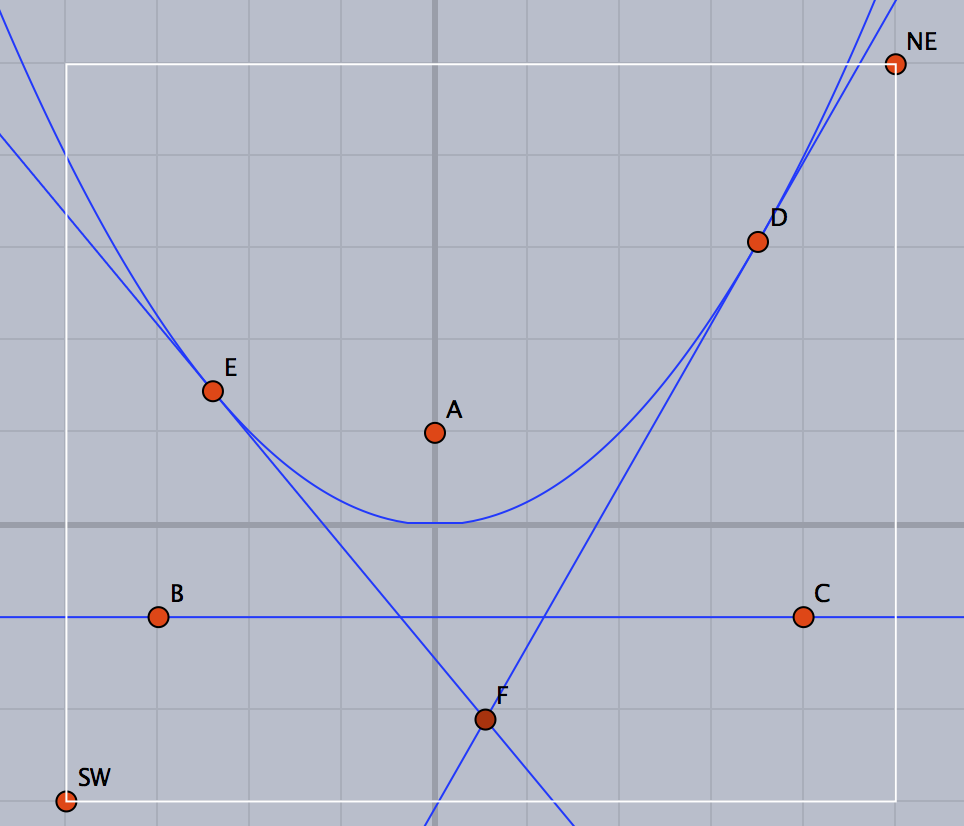
\includegraphics[bb=0 0 964 826 , width=6cm]{Fig/parabolaplot.png}\\
 \\
 以上で作図ができたので,次のスクリプトを書いて実行する。
\begin{verbatim}
  Parabolaplot("1",[A,B,C]); 
  Lineplot([D,F]);
  Lineplot([E,F]);
  Listplot([E,F,D]);
  Hatchdata("1",["ii"],[["gr1para","s"],["sgEFD","n"]]);
\end{verbatim}
 \\
 これで,次図ができる。このあと,文字などは適当に追加する。\\
 \\
           %%% fig.tex 2015-8-3 20:14
%%% fig.sce 2015-8-3 20:14
{\unitlength=4mm%
\begin{picture}%
(   9.00000,   8.00000)(  -4.00000,  -3.00000)%
\special{pn 8}%
%
\special{pa -630 -630}\special{pa -627 -624}\special{pa -595 -561}\special{pa -562 -502}%
\special{pa -530 -446}\special{pa -498 -394}\special{pa -466 -345}\special{pa -434 -299}%
\special{pa -402 -256}\special{pa -370 -217}\special{pa -337 -181}\special{pa -305 -148}%
\special{pa -273 -118}\special{pa -241 -92}\special{pa -209 -69}\special{pa -177 -50}%
\special{pa -145 -33}\special{pa -112 -20}\special{pa -80 -10}\special{pa -48 -4}%
\special{pa -16 0}\special{pa 16 0}\special{pa 48 -4}\special{pa 80 -10}\special{pa 112 -20}%
\special{pa 145 -33}\special{pa 177 -50}\special{pa 209 -69}\special{pa 241 -92}\special{pa 273 -118}%
\special{pa 305 -148}\special{pa 337 -181}\special{pa 370 -217}\special{pa 402 -256}%
\special{pa 434 -299}\special{pa 466 -345}\special{pa 498 -394}\special{pa 530 -446}%
\special{pa 562 -502}\special{pa 595 -561}\special{pa 627 -624}\special{pa 659 -689}%
\special{pa 691 -758}\special{pa 704 -787}%
\special{fp}%
\special{pa 725 -787}\special{pa 6 472}%
\special{fp}%
\special{pa -630 -530}\special{pa 202 472}%
\special{fp}%
\special{pa -379 -229}\special{pa 86 333}\special{pa 552 -484}%
\special{fp}%
\special{pa 75 319}\special{pa 119 276}%
\special{fp}%
\special{pa 63 304}\special{pa 156 211}%
\special{fp}%
\special{pa 50 289}\special{pa 193 146}%
\special{fp}%
\special{pa 37 274}\special{pa 229 82}%
\special{fp}%
\special{pa 25 258}\special{pa 266 17}%
\special{fp}%
\special{pa 12 243}\special{pa 303 -48}%
\special{fp}%
\special{pa -1 228}\special{pa 340 -113}%
\special{fp}%
\special{pa -13 213}\special{pa 377 -178}%
\special{fp}%
\special{pa -26 198}\special{pa 414 -243}%
\special{fp}%
\special{pa -38 182}\special{pa 224 -80}%
\special{fp}%
\special{pa 407 -263}\special{pa 451 -307}%
\special{fp}%
\special{pa -51 167}\special{pa 154 -38}%
\special{fp}%
\special{pa 476 -360}\special{pa 488 -372}%
\special{fp}%
\special{pa -64 152}\special{pa 107 -18}%
\special{fp}%
\special{pa 523 -435}\special{pa 525 -437}%
\special{fp}%
\special{pa -76 137}\special{pa 68 -8}%
\special{fp}%
\special{pa -89 121}\special{pa 35 -2}%
\special{fp}%
\special{pa -102 106}\special{pa 5 0}%
\special{fp}%
\special{pa -114 91}\special{pa -22 -1}%
\special{fp}%
\special{pa -127 76}\special{pa -47 -4}%
\special{fp}%
\special{pa -139 61}\special{pa -71 -8}%
\special{fp}%
\special{pa -152 45}\special{pa -93 -14}%
\special{fp}%
\special{pa -165 30}\special{pa -114 -21}%
\special{fp}%
\special{pa -177 15}\special{pa -134 -29}%
\special{fp}%
\special{pa -190 0}\special{pa -153 -37}%
\special{fp}%
\special{pa -203 -15}\special{pa -171 -47}%
\special{fp}%
\special{pa -215 -31}\special{pa -189 -57}%
\special{fp}%
\special{pa -228 -46}\special{pa -206 -68}%
\special{fp}%
\special{pa -240 -61}\special{pa -222 -79}%
\special{fp}%
\special{pa -253 -76}\special{pa -239 -91}%
\special{fp}%
\special{pa -266 -91}\special{pa -254 -103}%
\special{fp}%
\special{pa -278 -107}\special{pa -269 -115}%
\special{fp}%
\special{pa -291 -122}\special{pa -284 -129}%
\special{fp}%
\special{pa -304 -137}\special{pa -299 -142}%
\special{fp}%
\special{pa -316 -152}\special{pa -313 -156}%
\special{fp}%
\special{pa -329 -168}\special{pa -327 -170}%
\special{fp}%
\special{pa -341 -183}\special{pa -340 -184}%
\special{fp}%
\special{pa -354 -198}\special{pa -353 -199}%
\special{fp}%
\special{pa -367 -213}\special{pa -366 -213}%
\special{fp}%
\special{pa -379 -228}\special{pa -379 -229}%
\special{fp}%
\special{pn 8}%
\special{pa -630 0}\special{pa 787 0}%
\special{fp}%
\special{pn 8}%
\special{pa 713 24}\special{pa 787 0}\special{pa 713 -24}\special{pa 713 0}\special{pa 713 24}%
\special{sh 1}\special{ip}%
\special{pn 8}%
\special{pa 713 24}\special{pa 787 0}\special{pa 713 -24}\special{pa 713 0}\special{pa 713 24}%
\special{fp}%
\special{pn 8}%
\special{pn 8}%
\special{pa 0 472}\special{pa 0 -787}%
\special{fp}%
\special{pn 8}%
\special{pa 24 -713}\special{pa 0 -787}\special{pa -24 -713}\special{pa 0 -713}\special{pa 24 -713}%
\special{sh 1}\special{ip}%
\special{pn 8}%
\special{pa 24 -713}\special{pa 0 -787}\special{pa -24 -713}\special{pa 0 -713}\special{pa 24 -713}%
\special{fp}%
\special{pn 8}%
\settowidth{\Width}{$x$}\setlength{\Width}{0\Width}%
\settoheight{\Height}{$x$}\settodepth{\Depth}{$x$}\setlength{\Height}{-0.5\Height}\setlength{\Depth}{0.5\Depth}\addtolength{\Height}{\Depth}%
\put(5.0500,0.0000){\hspace*{\Width}\raisebox{\Height}{$x$}}%
%
%
\settowidth{\Width}{$y$}\setlength{\Width}{-0.5\Width}%
\settoheight{\Height}{$y$}\settodepth{\Depth}{$y$}\setlength{\Height}{\Depth}%
\put(0.0000,5.0500){\hspace*{\Width}\raisebox{\Height}{$y$}}%
%
%
\settowidth{\Width}{O}\setlength{\Width}{-1\Width}%
\settoheight{\Height}{O}\settodepth{\Depth}{O}\setlength{\Height}{-\Height}%
\put(-0.0500,-0.0500){\hspace*{\Width}\raisebox{\Height}{O}}%
%
%
\end{picture}}%
 \\
\begin{flushright} \hyperlink{functionlist}{$\Rightarrow$関数一覧}\end{flushright}
 \\
\hypertarget{ovaldata}{}
\item[関数] Ovaldata(name, 点リスト,options)
\item[機能] 角を丸くした矩形を描く
\item[説明] 中心と対角の1点を指定し,角を丸くした矩形を描く\\
 optionsは,角の落とし具合と線種など。デフォルトは0.2 \\

例:いくつかの例を示す。
\begin{verbatim}
  Ovaldata("1", [A,B]);
  Ovaldata("2", [C,D],[0]);
  Ovaldata("3", [E,F],[1,"dr,3"]);
  Ovaldata("4", [G,H],[1.5,"da"]);
\end{verbatim}
 %%% test.tex 2014-11-30 22:38
%%% test.sce 2014-11-30 22:38
{\unitlength=5mm%
\begin{picture}%
(  21.04000,   5.44000)(  -3.04000,   0.56000)%
\special{pn 8}%
%
\special{pn 24}%
\special{pa 2268 -591}\special{pa 2268 -803}\special{pa 2265 -834}\special{pa 2258 -864}%
\special{pa 2246 -893}\special{pa 2230 -919}\special{pa 2210 -942}\special{pa 2187 -962}%
\special{pa 2160 -979}\special{pa 2132 -990}\special{pa 2102 -998}\special{pa 2071 -1000}%
\special{pa 1969 -1000}\special{pa 1866 -1000}\special{pa 1835 -998}\special{pa 1805 -990}%
\special{pa 1777 -979}\special{pa 1750 -962}\special{pa 1727 -942}\special{pa 1707 -919}%
\special{pa 1691 -893}\special{pa 1679 -864}\special{pa 1672 -834}\special{pa 1669 -803}%
\special{pa 1669 -591}\special{pa 1669 -378}\special{pa 1672 -347}\special{pa 1679 -317}%
\special{pa 1691 -289}\special{pa 1707 -262}\special{pa 1727 -239}\special{pa 1750 -219}%
\special{pa 1777 -203}\special{pa 1805 -191}\special{pa 1835 -184}\special{pa 1866 -181}%
\special{pa 1969 -181}\special{pa 2071 -181}\special{pa 2102 -184}\special{pa 2132 -191}%
\special{pa 2160 -203}\special{pa 2187 -219}\special{pa 2210 -239}\special{pa 2230 -262}%
\special{pa 2246 -289}\special{pa 2258 -317}\special{pa 2265 -347}\special{pa 2268 -378}%
\special{pa 2268 -591}%
\special{fp}%
\special{pn 8}%
\special{pa 3354 -591}\special{pa 3354 -602}\special{pa 3352 -629}\special{fp}\special{pa 3346 -667}\special{pa 3340 -694}\special{pa 3335 -705}\special{fp}%
\special{pa 3320 -740}\special{pa 3300 -773}\special{fp}\special{pa 3275 -803}\special{pa 3268 -811}\special{pa 3247 -829}\special{fp}%
\special{pa 3215 -852}\special{pa 3193 -865}\special{pa 3181 -870}\special{fp}\special{pa 3145 -884}\special{pa 3108 -893}\special{fp}%
\special{pa 3069 -897}\special{pa 3059 -898}\special{pa 3030 -898}\special{fp}\special{pa 2992 -898}\special{pa 2953 -898}\special{pa 2953 -898}\special{fp}%
\special{pa 2914 -898}\special{pa 2875 -898}\special{fp}\special{pa 2836 -897}\special{pa 2800 -894}\special{pa 2798 -893}\special{fp}%
\special{pa 2760 -884}\special{pa 2755 -883}\special{pa 2724 -870}\special{fp}\special{pa 2690 -852}\special{pa 2673 -841}\special{pa 2659 -829}\special{fp}%
\special{pa 2631 -803}\special{pa 2608 -776}\special{pa 2606 -773}\special{fp}\special{pa 2586 -740}\special{pa 2583 -736}\special{pa 2570 -705}\special{fp}%
\special{pa 2559 -667}\special{pa 2555 -649}\special{pa 2553 -629}\special{fp}\special{pa 2551 -591}\special{pa 2551 -579}\special{pa 2553 -552}\special{fp}%
\special{pa 2559 -514}\special{pa 2566 -487}\special{pa 2570 -477}\special{fp}\special{pa 2586 -441}\special{pa 2606 -408}\special{fp}%
\special{pa 2631 -378}\special{pa 2638 -370}\special{pa 2659 -352}\special{fp}\special{pa 2690 -329}\special{pa 2712 -316}\special{pa 2724 -311}\special{fp}%
\special{pa 2760 -297}\special{pa 2798 -288}\special{fp}\special{pa 2836 -284}\special{pa 2846 -283}\special{pa 2875 -283}\special{fp}%
\special{pa 2914 -283}\special{pa 2953 -283}\special{pa 2953 -283}\special{fp}\special{pa 2992 -283}\special{pa 3030 -283}\special{fp}%
\special{pa 3069 -284}\special{pa 3105 -287}\special{pa 3108 -288}\special{fp}\special{pa 3145 -297}\special{pa 3150 -298}\special{pa 3181 -311}\special{fp}%
\special{pa 3215 -329}\special{pa 3233 -340}\special{pa 3247 -352}\special{fp}\special{pa 3275 -378}\special{pa 3298 -405}\special{pa 3300 -408}\special{fp}%
\special{pa 3320 -441}\special{pa 3322 -445}\special{pa 3335 -477}\special{fp}\special{pa 3346 -514}\special{pa 3351 -533}\special{pa 3352 -552}\special{fp}%
%
%
\special{pa 8 -599}\special{pa 2 -602}\special{pa -5 -601}\special{pa -11 -596}\special{pa -12 -589}%
\special{pa -8 -582}\special{pa -2 -579}\special{pa 5 -580}\special{pa 11 -585}\special{pa 12 -592}%
\special{pa 8 -599}\special{sh 1}\special{fp}%
\special{pa 402 -993}\special{pa 396 -996}\special{pa 388 -995}\special{pa 383 -990}%
\special{pa 382 -982}\special{pa 385 -976}\special{pa 392 -973}\special{pa 399 -974}%
\special{pa 404 -979}\special{pa 405 -986}\special{pa 402 -993}\special{sh 1}\special{fp}%
\special{pa 993 -599}\special{pa 986 -602}\special{pa 979 -601}\special{pa 974 -596}%
\special{pa 973 -589}\special{pa 976 -582}\special{pa 982 -579}\special{pa 990 -580}%
\special{pa 995 -585}\special{pa 996 -592}\special{pa 993 -599}\special{sh 1}\special{fp}%
\special{pa 1386 -402}\special{pa 1380 -405}\special{pa 1373 -404}\special{pa 1367 -399}%
\special{pa 1366 -392}\special{pa 1370 -385}\special{pa 1376 -382}\special{pa 1383 -383}%
\special{pa 1388 -388}\special{pa 1390 -396}\special{pa 1386 -402}\special{sh 1}\special{fp}%
\special{pa 1977 -599}\special{pa 1970 -602}\special{pa 1963 -601}\special{pa 1958 -596}%
\special{pa 1957 -589}\special{pa 1960 -582}\special{pa 1967 -579}\special{pa 1974 -580}%
\special{pa 1979 -585}\special{pa 1980 -592}\special{pa 1977 -599}\special{sh 1}\special{fp}%
\special{pa 1678 -1008}\special{pa 1671 -1012}\special{pa 1664 -1011}\special{pa 1659 -1005}%
\special{pa 1658 -998}\special{pa 1661 -992}\special{pa 1667 -988}\special{pa 1675 -989}%
\special{pa 1680 -995}\special{pa 1681 -1002}\special{pa 1678 -1008}\special{sh 1}\special{fp}%
\special{pa 2961 -599}\special{pa 2955 -602}\special{pa 2947 -601}\special{pa 2942 -596}%
\special{pa 2941 -589}\special{pa 2944 -582}\special{pa 2951 -579}\special{pa 2958 -580}%
\special{pa 2963 -585}\special{pa 2964 -592}\special{pa 2961 -599}\special{sh 1}\special{fp}%
\special{pa 3363 -906}\special{pa 3356 -909}\special{pa 3349 -908}\special{pa 3344 -903}%
\special{pa 3343 -896}\special{pa 3346 -889}\special{pa 3352 -886}\special{pa 3360 -887}%
\special{pa 3365 -892}\special{pa 3366 -899}\special{pa 3363 -906}\special{sh 1}\special{fp}%
\settowidth{\Width}{A}\setlength{\Width}{0\Width}%
\settoheight{\Height}{A}\settodepth{\Depth}{A}\setlength{\Height}{\Depth}%
\put(0.0500,3.0500){\hspace*{\Width}\raisebox{\Height}{A}}%
%
%
\settowidth{\Width}{B}\setlength{\Width}{0\Width}%
\settoheight{\Height}{B}\settodepth{\Depth}{B}\setlength{\Height}{\Depth}%
\put(2.0500,5.0500){\hspace*{\Width}\raisebox{\Height}{B}}%
%
%
\settowidth{\Width}{C}\setlength{\Width}{0\Width}%
\settoheight{\Height}{C}\settodepth{\Depth}{C}\setlength{\Height}{\Depth}%
\put(5.0500,3.0500){\hspace*{\Width}\raisebox{\Height}{C}}%
%
%
\settowidth{\Width}{D}\setlength{\Width}{0\Width}%
\settoheight{\Height}{D}\settodepth{\Depth}{D}\setlength{\Height}{-\Height}%
\put(7.0500,1.9500){\hspace*{\Width}\raisebox{\Height}{D}}%
%
%
\settowidth{\Width}{E}\setlength{\Width}{0\Width}%
\settoheight{\Height}{E}\settodepth{\Depth}{E}\setlength{\Height}{\Depth}%
\put(10.0500,3.0500){\hspace*{\Width}\raisebox{\Height}{E}}%
%
%
\settowidth{\Width}{F}\setlength{\Width}{-1\Width}%
\settoheight{\Height}{F}\settodepth{\Depth}{F}\setlength{\Height}{\Depth}%
\put(8.4300,5.1300){\hspace*{\Width}\raisebox{\Height}{F}}%
%
%
\settowidth{\Width}{G}\setlength{\Width}{0\Width}%
\settoheight{\Height}{G}\settodepth{\Depth}{G}\setlength{\Height}{\Depth}%
\put(15.0500,3.0500){\hspace*{\Width}\raisebox{\Height}{G}}%
%
%
\settowidth{\Width}{H}\setlength{\Width}{0\Width}%
\settoheight{\Height}{H}\settodepth{\Depth}{H}\setlength{\Height}{\Depth}%
\put(17.0900,4.6100){\hspace*{\Width}\raisebox{\Height}{H}}%
%
%
\special{pa 394 -591}\special{pa 394 -945}\special{pa 393 -951}\special{pa 392 -957}%
\special{pa 389 -963}\special{pa 386 -968}\special{pa 382 -973}\special{pa 377 -977}%
\special{pa 372 -980}\special{pa 366 -982}\special{pa 360 -984}\special{pa 354 -984}%
\special{pa 0 -984}\special{pa -354 -984}\special{pa -360 -984}\special{pa -366 -982}%
\special{pa -372 -980}\special{pa -377 -977}\special{pa -382 -973}\special{pa -386 -968}%
\special{pa -389 -963}\special{pa -392 -957}\special{pa -393 -951}\special{pa -394 -945}%
\special{pa -394 -591}\special{pa -394 -236}\special{pa -393 -230}\special{pa -392 -224}%
\special{pa -389 -218}\special{pa -386 -213}\special{pa -382 -208}\special{pa -377 -204}%
\special{pa -372 -201}\special{pa -366 -199}\special{pa -360 -197}\special{pa -354 -197}%
\special{pa 0 -197}\special{pa 354 -197}\special{pa 360 -197}\special{pa 366 -199}%
\special{pa 372 -201}\special{pa 377 -204}\special{pa 382 -208}\special{pa 386 -213}%
\special{pa 389 -218}\special{pa 392 -224}\special{pa 393 -230}\special{pa 394 -236}%
\special{pa 394 -591}%
\special{fp}%
\special{pa 1378 -591}\special{pa 1378 -787}\special{pa 984 -787}\special{pa 591 -787}%
\special{pa 591 -591}\special{pa 591 -394}\special{pa 984 -394}\special{pa 1378 -394}%
\special{pa 1378 -591}%
\special{fp}%
\end{picture}}%\\
 \\
\begin{flushright} \hyperlink{functionlist}{$\Rightarrow$関数一覧}\end{flushright}

\hypertarget{htickmark}{}
\item[関数] Htickmark([横座標 , 方向 , 文字])
\item[機能] 横軸に目盛を書く。
\item[説明] Scilabのみで実行する。Cinderellaの描画面には反映されない。引数は位置(横座標),方向,文字。複数点の情報を[ ]内にまとめて記入できる。\\

例 点$(2,\ 0)$の南西側に$2$を表示する。\\
  \verb|Htickmark([2,"sw","2"]);|\\

例 -5から5までの目盛を打つ。\\
 Cindyscriptのリスト処理を使って,次のように引数のリストを作って渡す。
\begin{verbatim}
  memori=apply(-5..5,x,[x,"s",text(x)]);
  memori=flatten(remove(memori,[[0,"s","0"]]));
  Htickmark(memori);
\end{verbatim}
 1行目,apply のカッコ内の -5..5 でリスト[-5,-4,-3,-2,-1,0,1,2,3,4,5] ができる。\\
 それを用いて,applyで[数, "s",数の文字] からなるリストができる。text(x) はxを文字にする関数。\\
 2行目で,このリストから,[0,"s","0"]を除き,リストを平滑化する。\\
 結果は次のようになる。\\

%%% test.tex 2014-11-11 13:14
%%% test.sce 2014-11-11 13:14
{\unitlength=6mm%
\begin{picture}%
(  12.00000,   6.00000)(  -6.00000,  -3.00000)%
\special{pn 8}%
%
\special{pa -1181 -20}\special{pa -1181 20}%
\special{fp}%
\settowidth{\Width}{$-5$}\setlength{\Width}{-0.5\Width}%
\settoheight{\Height}{$-5$}\settodepth{\Depth}{$-5$}\setlength{\Height}{-\Height}%
\put(-5.0000,-0.1333){\hspace*{\Width}\raisebox{\Height}{$-5$}}%
%
%
%
\special{pa -945 -20}\special{pa -945 20}%
\special{fp}%
\settowidth{\Width}{$-4$}\setlength{\Width}{-0.5\Width}%
\settoheight{\Height}{$-4$}\settodepth{\Depth}{$-4$}\setlength{\Height}{-\Height}%
\put(-4.0000,-0.1333){\hspace*{\Width}\raisebox{\Height}{$-4$}}%
%
%
%
\special{pa -709 -20}\special{pa -709 20}%
\special{fp}%
\settowidth{\Width}{$-3$}\setlength{\Width}{-0.5\Width}%
\settoheight{\Height}{$-3$}\settodepth{\Depth}{$-3$}\setlength{\Height}{-\Height}%
\put(-3.0000,-0.1333){\hspace*{\Width}\raisebox{\Height}{$-3$}}%
%
%
%
\special{pa -472 -20}\special{pa -472 20}%
\special{fp}%
\settowidth{\Width}{$-2$}\setlength{\Width}{-0.5\Width}%
\settoheight{\Height}{$-2$}\settodepth{\Depth}{$-2$}\setlength{\Height}{-\Height}%
\put(-2.0000,-0.1333){\hspace*{\Width}\raisebox{\Height}{$-2$}}%
%
%
%
\special{pa -236 -20}\special{pa -236 20}%
\special{fp}%
\settowidth{\Width}{$-1$}\setlength{\Width}{-0.5\Width}%
\settoheight{\Height}{$-1$}\settodepth{\Depth}{$-1$}\setlength{\Height}{-\Height}%
\put(-1.0000,-0.1333){\hspace*{\Width}\raisebox{\Height}{$-1$}}%
%
%
%
\special{pa 236 -20}\special{pa 236 20}%
\special{fp}%
\settowidth{\Width}{$1$}\setlength{\Width}{-0.5\Width}%
\settoheight{\Height}{$1$}\settodepth{\Depth}{$1$}\setlength{\Height}{-\Height}%
\put(1.0000,-0.1333){\hspace*{\Width}\raisebox{\Height}{$1$}}%
%
%
%
\special{pa 472 -20}\special{pa 472 20}%
\special{fp}%
\settowidth{\Width}{$2$}\setlength{\Width}{-0.5\Width}%
\settoheight{\Height}{$2$}\settodepth{\Depth}{$2$}\setlength{\Height}{-\Height}%
\put(2.0000,-0.1333){\hspace*{\Width}\raisebox{\Height}{$2$}}%
%
%
%
\special{pa 709 -20}\special{pa 709 20}%
\special{fp}%
\settowidth{\Width}{$3$}\setlength{\Width}{-0.5\Width}%
\settoheight{\Height}{$3$}\settodepth{\Depth}{$3$}\setlength{\Height}{-\Height}%
\put(3.0000,-0.1333){\hspace*{\Width}\raisebox{\Height}{$3$}}%
%
%
%
\special{pa 945 -20}\special{pa 945 20}%
\special{fp}%
\settowidth{\Width}{$4$}\setlength{\Width}{-0.5\Width}%
\settoheight{\Height}{$4$}\settodepth{\Depth}{$4$}\setlength{\Height}{-\Height}%
\put(4.0000,-0.1333){\hspace*{\Width}\raisebox{\Height}{$4$}}%
%
%
%
\special{pa 1181 -20}\special{pa 1181 20}%
\special{fp}%
\settowidth{\Width}{$5$}\setlength{\Width}{-0.5\Width}%
\settoheight{\Height}{$5$}\settodepth{\Depth}{$5$}\setlength{\Height}{-\Height}%
\put(5.0000,-0.1333){\hspace*{\Width}\raisebox{\Height}{$5$}}%
%
%
%
\special{pn 8}%
\special{pa -1417 0}\special{pa 1417 0}%
\special{fp}%
\special{pn 8}%
\special{pa 1342 24}\special{pa 1417 0}\special{pa 1342 -24}\special{pa 1342 0}\special{pa 1342 24}%
\special{sh 1}\special{ip}%
\special{pn 8}%
\special{pa 1342 24}\special{pa 1417 0}\special{pa 1342 -24}\special{pa 1342 0}\special{pa 1342 24}%
\special{fp}%
\special{pn 8}%
\special{pn 8}%
\special{pa 0 709}\special{pa 0 -709}%
\special{fp}%
\special{pn 8}%
\special{pa 24 -634}\special{pa 0 -709}\special{pa -24 -634}\special{pa 0 -634}\special{pa 24 -634}%
\special{sh 1}\special{ip}%
\special{pn 8}%
\special{pa 24 -634}\special{pa 0 -709}\special{pa -24 -634}\special{pa 0 -634}\special{pa 24 -634}%
\special{fp}%
\special{pn 8}%
\settowidth{\Width}{$x$}\setlength{\Width}{0\Width}%
\settoheight{\Height}{$x$}\settodepth{\Depth}{$x$}\setlength{\Height}{-0.5\Height}\setlength{\Depth}{0.5\Depth}\addtolength{\Height}{\Depth}%
\put(6.0500,0.0000){\hspace*{\Width}\raisebox{\Height}{$x$}}%
%
%
\settowidth{\Width}{$y$}\setlength{\Width}{-0.5\Width}%
\settoheight{\Height}{$y$}\settodepth{\Depth}{$y$}\setlength{\Height}{\Depth}%
\put(0.0000,3.0500){\hspace*{\Width}\raisebox{\Height}{$y$}}%
%
%
\settowidth{\Width}{O}\setlength{\Width}{-1\Width}%
\settoheight{\Height}{O}\settodepth{\Depth}{O}\setlength{\Height}{-\Height}%
\put(-0.0500,-0.0500){\hspace*{\Width}\raisebox{\Height}{O}}%
%
%
\end{picture}}%\\

\hypertarget{vtickmark}{}
\item[関数] Vtickmark([横座標 , 方向 , 文字])
\item[機能] 縦軸に目盛を書く。
\item[説明] Htickmarkと同様。縦軸に目盛を書く。\\

例:点$(0,\ 1),\ (0,\ 2)$の西側に$1,\ 2$を表示する。\\
  \verb|Htickmark([1,"w","1",2,"w","2"]);|\\
\\

\begin{flushright} \hyperlink{functionlist}{$\Rightarrow$関数一覧}\end{flushright}

\hypertarget{implicitplot}{}
\item[関数] Implicitplot(name,式,xの定義域,yの定義域, options)
\item[機能] 陰関数のグラフを描く。
\item[説明] 陰関数の式を与えてグラフを描く。式,定義域とも文字列。\\
 options は,"r","m","Wait=n" が指定できる。Wait の初期値は10。\\
 "r","m"に関しては,オプションなしまたは,”” のとき\\
  i) データファイルがなければ,新しく作る\\
  ii) データファイルが既にあればそれを読み込む\\
 "m"  のとき,強制的にデータファイルを作り直す。\\
 "r" のとき,すでにあるデータファイルを読み込む。\\ 

例:楕円を描いて,中にハッチをかける。
\begin{verbatim}
  Implicitplot("1","x^2+2*y^2=4","x=[-2,2]","y=[-2,2]");
  Hatchdata("1","i",["imp1"]);
\end{verbatim}
 注)ここで,yの定義域は実際より広くとってある。"y=[-1,1]" とすると,上下が欠けた楕円になる。曲線だけならそれでよいが,その場合,閉曲線ではないのでHatchdata() で無用に時間がかかってしまうので要注意。\\
 \\

\hypertarget{letter}{}\item[関数] Letter([位置, 方向, 文字列])
\item[機能] 文字列を表示する
\item[説明] 「位置(座標)」と方向で指定された場所に文字を書き込む。\\
 位置(座標)は点の名前で指定することもできる。場所は上下左右中央( n/s/w/e/c )の方向で表す。(n/s/w/e は東西南北の記号)\\
 \\
       %%% letter4.tex 2014-11-20 9:17
%%% sampleu3.sce 2014-11-17 19:14
{\unitlength=1cm%
\begin{picture}%
(   9.97000,   4.53000)(  -5.83000,  -2.11000)%
\special{pn 8}%
%
\normalsize%
\settowidth{\Width}{w}\setlength{\Width}{-0.5\Width}%
\settoheight{\Height}{w}\settodepth{\Depth}{w}\setlength{\Height}{-0.5\Height}\setlength{\Depth}{0.5\Depth}\addtolength{\Height}{\Depth}%
\put(-3.0000,0.0000){\hspace*{\Width}\raisebox{\Height}{w}}%
%
%
\settowidth{\Width}{e}\setlength{\Width}{-0.5\Width}%
\settoheight{\Height}{e}\settodepth{\Depth}{e}\setlength{\Height}{-0.5\Height}\setlength{\Depth}{0.5\Depth}\addtolength{\Height}{\Depth}%
\put(-1.0000,0.0000){\hspace*{\Width}\raisebox{\Height}{e}}%
%
%
\settowidth{\Width}{s}\setlength{\Width}{-0.5\Width}%
\settoheight{\Height}{s}\settodepth{\Depth}{s}\setlength{\Height}{-0.5\Height}\setlength{\Depth}{0.5\Depth}\addtolength{\Height}{\Depth}%
\put(-2.0000,-1.0000){\hspace*{\Width}\raisebox{\Height}{s}}%
%
%
\settowidth{\Width}{n}\setlength{\Width}{-0.5\Width}%
\settoheight{\Height}{n}\settodepth{\Depth}{n}\setlength{\Height}{-0.5\Height}\setlength{\Depth}{0.5\Depth}\addtolength{\Height}{\Depth}%
\put(-2.0000,1.0000){\hspace*{\Width}\raisebox{\Height}{n}}%
%
%
\settowidth{\Width}{w2}\setlength{\Width}{-0.5\Width}%
\settoheight{\Height}{w2}\settodepth{\Depth}{w2}\setlength{\Height}{-0.5\Height}\setlength{\Depth}{0.5\Depth}\addtolength{\Height}{\Depth}%
\put(-4.0000,0.0100){\hspace*{\Width}\raisebox{\Height}{w2}}%
%
%
\settowidth{\Width}{e2}\setlength{\Width}{-0.5\Width}%
\settoheight{\Height}{e2}\settodepth{\Depth}{e2}\setlength{\Height}{-0.5\Height}\setlength{\Depth}{0.5\Depth}\addtolength{\Height}{\Depth}%
\put(-0.0300,0.0100){\hspace*{\Width}\raisebox{\Height}{e2}}%
%
%
\settowidth{\Width}{c}\setlength{\Width}{-0.5\Width}%
\settoheight{\Height}{c}\settodepth{\Depth}{c}\setlength{\Height}{-0.5\Height}\setlength{\Depth}{0.5\Depth}\addtolength{\Height}{\Depth}%
\put(-2.0000,0.0000){\hspace*{\Width}\raisebox{\Height}{c}}%
%
%
\settowidth{\Width}{nw}\setlength{\Width}{-0.5\Width}%
\settoheight{\Height}{nw}\settodepth{\Depth}{nw}\setlength{\Height}{-0.5\Height}\setlength{\Depth}{0.5\Depth}\addtolength{\Height}{\Depth}%
\put(-2.7800,0.7300){\hspace*{\Width}\raisebox{\Height}{nw}}%
%
%
\settowidth{\Width}{sw}\setlength{\Width}{-0.5\Width}%
\settoheight{\Height}{sw}\settodepth{\Depth}{sw}\setlength{\Height}{-0.5\Height}\setlength{\Depth}{0.5\Depth}\addtolength{\Height}{\Depth}%
\put(-2.8100,-0.8100){\hspace*{\Width}\raisebox{\Height}{sw}}%
%
%
\settowidth{\Width}{ne}\setlength{\Width}{-0.5\Width}%
\settoheight{\Height}{ne}\settodepth{\Depth}{ne}\setlength{\Height}{-0.5\Height}\setlength{\Depth}{0.5\Depth}\addtolength{\Height}{\Depth}%
\put(-1.1600,0.8200){\hspace*{\Width}\raisebox{\Height}{ne}}%
%
%
\settowidth{\Width}{n2w2}\setlength{\Width}{-0.5\Width}%
\settoheight{\Height}{n2w2}\settodepth{\Depth}{n2w2}\setlength{\Height}{-0.5\Height}\setlength{\Depth}{0.5\Depth}\addtolength{\Height}{\Depth}%
\put(-3.6300,1.3800){\hspace*{\Width}\raisebox{\Height}{n2w2}}%
%
%
\settowidth{\Width}{e4}\setlength{\Width}{-0.5\Width}%
\settoheight{\Height}{e4}\settodepth{\Depth}{e4}\setlength{\Height}{-0.5\Height}\setlength{\Depth}{0.5\Depth}\addtolength{\Height}{\Depth}%
\put(1.9100,-0.0100){\hspace*{\Width}\raisebox{\Height}{e4}}%
%
%
\settowidth{\Width}{se}\setlength{\Width}{-0.5\Width}%
\settoheight{\Height}{se}\settodepth{\Depth}{se}\setlength{\Height}{-0.5\Height}\setlength{\Depth}{0.5\Depth}\addtolength{\Height}{\Depth}%
\put(-1.1700,-0.7800){\hspace*{\Width}\raisebox{\Height}{se}}%
%
%
\settowidth{\Width}{w3}\setlength{\Width}{-0.5\Width}%
\settoheight{\Height}{w3}\settodepth{\Depth}{w3}\setlength{\Height}{-0.5\Height}\setlength{\Depth}{0.5\Depth}\addtolength{\Height}{\Depth}%
\put(-4.6000,0.0100){\hspace*{\Width}\raisebox{\Height}{w3}}%
%
%
\settowidth{\Width}{w4}\setlength{\Width}{-0.5\Width}%
\settoheight{\Height}{w4}\settodepth{\Depth}{w4}\setlength{\Height}{-0.5\Height}\setlength{\Depth}{0.5\Depth}\addtolength{\Height}{\Depth}%
\put(-5.4000,0.0200){\hspace*{\Width}\raisebox{\Height}{w4}}%
%
%
\settowidth{\Width}{s2}\setlength{\Width}{-0.5\Width}%
\settoheight{\Height}{s2}\settodepth{\Depth}{s2}\setlength{\Height}{-0.5\Height}\setlength{\Depth}{0.5\Depth}\addtolength{\Height}{\Depth}%
\put(-1.9900,-1.2700){\hspace*{\Width}\raisebox{\Height}{s2}}%
%
%
\settowidth{\Width}{s3}\setlength{\Width}{-0.5\Width}%
\settoheight{\Height}{s3}\settodepth{\Depth}{s3}\setlength{\Height}{-0.5\Height}\setlength{\Depth}{0.5\Depth}\addtolength{\Height}{\Depth}%
\put(-1.9900,-1.5700){\hspace*{\Width}\raisebox{\Height}{s3}}%
%
%
\settowidth{\Width}{n2}\setlength{\Width}{-0.5\Width}%
\settoheight{\Height}{n2}\settodepth{\Depth}{n2}\setlength{\Height}{-0.5\Height}\setlength{\Depth}{0.5\Depth}\addtolength{\Height}{\Depth}%
\put(-2.0000,1.3800){\hspace*{\Width}\raisebox{\Height}{n2}}%
%
%
\settowidth{\Width}{n3}\setlength{\Width}{-0.5\Width}%
\settoheight{\Height}{n3}\settodepth{\Depth}{n3}\setlength{\Height}{-0.5\Height}\setlength{\Depth}{0.5\Depth}\addtolength{\Height}{\Depth}%
\put(-2.0000,1.7600){\hspace*{\Width}\raisebox{\Height}{n3}}%
%
%
\settowidth{\Width}{s4}\setlength{\Width}{-0.5\Width}%
\settoheight{\Height}{s4}\settodepth{\Depth}{s4}\setlength{\Height}{-0.5\Height}\setlength{\Depth}{0.5\Depth}\addtolength{\Height}{\Depth}%
\put(-1.9800,-1.9200){\hspace*{\Width}\raisebox{\Height}{s4}}%
%
%
\settowidth{\Width}{n4}\setlength{\Width}{-0.5\Width}%
\settoheight{\Height}{n4}\settodepth{\Depth}{n4}\setlength{\Height}{-0.5\Height}\setlength{\Depth}{0.5\Depth}\addtolength{\Height}{\Depth}%
\put(-1.9800,2.0900){\hspace*{\Width}\raisebox{\Height}{n4}}%
%
%
\settowidth{\Width}{s2w2}\setlength{\Width}{-0.5\Width}%
\settoheight{\Height}{s2w2}\settodepth{\Depth}{s2w2}\setlength{\Height}{-0.5\Height}\setlength{\Depth}{0.5\Depth}\addtolength{\Height}{\Depth}%
\put(-3.6300,-1.4400){\hspace*{\Width}\raisebox{\Height}{s2w2}}%
%
%
\settowidth{\Width}{s2e2}\setlength{\Width}{-0.5\Width}%
\settoheight{\Height}{s2e2}\settodepth{\Depth}{s2e2}\setlength{\Height}{-0.5\Height}\setlength{\Depth}{0.5\Depth}\addtolength{\Height}{\Depth}%
\put(-0.2900,-1.4300){\hspace*{\Width}\raisebox{\Height}{s2e2}}%
%
%
\settowidth{\Width}{n2e2}\setlength{\Width}{-0.5\Width}%
\settoheight{\Height}{n2e2}\settodepth{\Depth}{n2e2}\setlength{\Height}{-0.5\Height}\setlength{\Depth}{0.5\Depth}\addtolength{\Height}{\Depth}%
\put(-0.2400,1.4500){\hspace*{\Width}\raisebox{\Height}{n2e2}}%
%
%
\settowidth{\Width}{ne2}\setlength{\Width}{-0.5\Width}%
\settoheight{\Height}{ne2}\settodepth{\Depth}{ne2}\setlength{\Height}{-0.5\Height}\setlength{\Depth}{0.5\Depth}\addtolength{\Height}{\Depth}%
\put(-0.2700,0.7400){\hspace*{\Width}\raisebox{\Height}{ne2}}%
%
%
\settowidth{\Width}{e3}\setlength{\Width}{-0.5\Width}%
\settoheight{\Height}{e3}\settodepth{\Depth}{e3}\setlength{\Height}{-0.5\Height}\setlength{\Depth}{0.5\Depth}\addtolength{\Height}{\Depth}%
\put(1.2300,0.0000){\hspace*{\Width}\raisebox{\Height}{e3}}%
%
%
\special{pn 8}%
\special{pa -925 4}\special{pa -1067 4}%
\special{fp}%
\special{pn 8}%
\special{pa -992 -20}\special{pa -1067 4}\special{pa -992 28}\special{pa -992 4}\special{pa -992 -20}%
\special{sh 1}\special{ip}%
\special{pn 8}%
\special{pa -992 -20}\special{pa -1067 4}\special{pa -992 28}\special{pa -992 4}\special{pa -992 -20}%
\special{fp}%
\special{pn 8}%
\special{pn 8}%
\special{pa -787 -130}\special{pa -787 -276}%
\special{fp}%
\special{pn 8}%
\special{pa -763 -201}\special{pa -787 -276}\special{pa -812 -201}\special{pa -787 -201}%
\special{pa -763 -201}\special{sh 1}\special{ip}%
\special{pn 8}%
\special{pa -763 -201}\special{pa -787 -276}\special{pa -812 -201}\special{pa -787 -201}%
\special{pa -763 -201}%
\special{fp}%
\special{pn 8}%
\special{pn 8}%
\special{pa -787 134}\special{pa -787 295}%
\special{fp}%
\special{pn 8}%
\special{pa -812 220}\special{pa -787 295}\special{pa -763 220}\special{pa -787 220}%
\special{pa -812 220}\special{sh 1}\special{ip}%
\special{pn 8}%
\special{pa -812 220}\special{pa -787 295}\special{pa -763 220}\special{pa -787 220}%
\special{pa -812 220}%
\special{fp}%
\special{pn 8}%
\special{pn 8}%
\special{pa -661 -12}\special{pa -520 -4}%
\special{fp}%
\special{pn 8}%
\special{pa -596 16}\special{pa -520 -4}\special{pa -593 -32}\special{pa -594 -8}%
\special{pa -596 16}\special{sh 1}\special{ip}%
\special{pn 8}%
\special{pa -596 16}\special{pa -520 -4}\special{pa -593 -32}\special{pa -594 -8}%
\special{pa -596 16}%
\special{fp}%
\special{pn 8}%
\special{pn 8}%
\special{pa -1311 -4}\special{pa -1437 -4}%
\special{fp}%
\special{pn 8}%
\special{pa -1362 -28}\special{pa -1437 -4}\special{pa -1362 20}\special{pa -1362 -4}%
\special{pa -1362 -28}\special{sh 1}\special{ip}%
\special{pn 8}%
\special{pa -1362 -28}\special{pa -1437 -4}\special{pa -1362 20}\special{pa -1362 -4}%
\special{pa -1362 -28}%
\special{fp}%
\special{pn 8}%
\special{pn 8}%
\special{pa -295 8}\special{pa -177 0}%
\special{fp}%
\special{pn 8}%
\special{pa -250 29}\special{pa -177 0}\special{pa -254 -19}\special{pa -252 5}\special{pa -250 29}%
\special{sh 1}\special{ip}%
\special{pn 8}%
\special{pa -250 29}\special{pa -177 0}\special{pa -254 -19}\special{pa -252 5}\special{pa -250 29}%
\special{fp}%
\special{pn 8}%
\special{pn 8}%
\special{pa 189 4}\special{pa 319 4}%
\special{fp}%
\special{pn 8}%
\special{pa 244 28}\special{pa 319 4}\special{pa 244 -20}\special{pa 244 4}\special{pa 244 28}%
\special{sh 1}\special{ip}%
\special{pn 8}%
\special{pa 244 28}\special{pa 319 4}\special{pa 244 -20}\special{pa 244 4}\special{pa 244 28}%
\special{fp}%
\special{pn 8}%
\special{pn 8}%
\special{pa -331 -402}\special{pa -213 -484}%
\special{fp}%
\special{pn 8}%
\special{pa -260 -421}\special{pa -213 -484}\special{pa -288 -461}\special{pa -274 -441}%
\special{pa -260 -421}\special{sh 1}\special{ip}%
\special{pn 8}%
\special{pa -260 -421}\special{pa -213 -484}\special{pa -288 -461}\special{pa -274 -441}%
\special{pa -260 -421}%
\special{fp}%
\special{pn 8}%
\special{pn 8}%
\special{pa -350 390}\special{pa -220 484}%
\special{fp}%
\special{pn 8}%
\special{pa -295 460}\special{pa -220 484}\special{pa -267 421}\special{pa -281 440}%
\special{pa -295 460}\special{sh 1}\special{ip}%
\special{pn 8}%
\special{pa -295 460}\special{pa -220 484}\special{pa -267 421}\special{pa -281 440}%
\special{pa -295 460}%
\special{fp}%
\special{pn 8}%
\special{pn 8}%
\special{pa -1181 390}\special{pa -1276 469}%
\special{fp}%
\special{pn 8}%
\special{pa -1234 402}\special{pa -1276 469}\special{pa -1202 439}\special{pa -1218 421}%
\special{pa -1234 402}\special{sh 1}\special{ip}%
\special{pn 8}%
\special{pa -1234 402}\special{pa -1276 469}\special{pa -1202 439}\special{pa -1218 421}%
\special{pa -1234 402}%
\special{fp}%
\special{pn 8}%
\special{pn 8}%
\special{pa -693 106}\special{pa -606 205}%
\special{fp}%
\special{pn 8}%
\special{pa -674 165}\special{pa -606 205}\special{pa -638 132}\special{pa -656 149}%
\special{pa -674 165}\special{sh 1}\special{ip}%
\special{pn 8}%
\special{pa -674 165}\special{pa -606 205}\special{pa -638 132}\special{pa -656 149}%
\special{pa -674 165}%
\special{fp}%
\special{pn 8}%
\special{pn 8}%
\special{pa -669 -106}\special{pa -594 -189}%
\special{fp}%
\special{pn 8}%
\special{pa -627 -117}\special{pa -594 -189}\special{pa -663 -150}\special{pa -645 -133}%
\special{pa -627 -117}\special{sh 1}\special{ip}%
\special{pn 8}%
\special{pa -627 -117}\special{pa -594 -189}\special{pa -663 -150}\special{pa -645 -133}%
\special{pa -627 -117}%
\special{fp}%
\special{pn 8}%
\special{pn 8}%
\special{pa -886 -87}\special{pa -1008 -205}%
\special{fp}%
\special{pn 8}%
\special{pa -937 -170}\special{pa -1008 -205}\special{pa -971 -135}\special{pa -954 -153}%
\special{pa -937 -170}\special{sh 1}\special{ip}%
\special{pn 8}%
\special{pa -937 -170}\special{pa -1008 -205}\special{pa -971 -135}\special{pa -954 -153}%
\special{pa -937 -170}%
\special{fp}%
\special{pn 8}%
\special{pn 8}%
\special{pa -917 122}\special{pa -992 220}%
\special{fp}%
\special{pn 8}%
\special{pa -966 146}\special{pa -992 220}\special{pa -927 176}\special{pa -947 161}%
\special{pa -966 146}\special{sh 1}\special{ip}%
\special{pn 8}%
\special{pa -966 146}\special{pa -992 220}\special{pa -927 176}\special{pa -947 161}%
\special{pa -966 146}%
\special{fp}%
\special{pn 8}%
\special{pn 8}%
\special{pa -1189 -370}\special{pa -1311 -457}%
\special{fp}%
\special{pn 8}%
\special{pa -1236 -433}\special{pa -1311 -457}\special{pa -1264 -394}\special{pa -1250 -413}%
\special{pa -1236 -433}\special{sh 1}\special{ip}%
\special{pn 8}%
\special{pa -1236 -433}\special{pa -1311 -457}\special{pa -1264 -394}\special{pa -1250 -413}%
\special{pa -1236 -433}%
\special{fp}%
\special{pn 8}%
\settowidth{\Width}{$\cdot$}\setlength{\Width}{-0.5\Width}%
\settoheight{\Height}{$\cdot$}\settodepth{\Depth}{$\cdot$}\setlength{\Height}{-0.5\Height}\setlength{\Depth}{0.5\Depth}\addtolength{\Height}{\Depth}%
\put(3.4200,-0.0100){\hspace*{\Width}\raisebox{\Height}{$\cdot$}}%
%
%
\settowidth{\Width}{$\cdot$}\setlength{\Width}{-1\Width}%
\settoheight{\Height}{$\cdot$}\settodepth{\Depth}{$\cdot$}\setlength{\Height}{-0.5\Height}\setlength{\Depth}{0.5\Depth}\addtolength{\Height}{\Depth}%
\put(3.3700,-0.0100){\hspace*{\Width}\raisebox{\Height}{$\cdot$}}%
%
%
\settowidth{\Width}{$\cdot$}\setlength{\Width}{0\Width}%
\settoheight{\Height}{$\cdot$}\settodepth{\Depth}{$\cdot$}\setlength{\Height}{-0.5\Height}\setlength{\Depth}{0.5\Depth}\addtolength{\Height}{\Depth}%
\put(3.4700,-0.0100){\hspace*{\Width}\raisebox{\Height}{$\cdot$}}%
%
%
\settowidth{\Width}{$\cdot$}\setlength{\Width}{-0.5\Width}%
\settoheight{\Height}{$\cdot$}\settodepth{\Depth}{$\cdot$}\setlength{\Height}{\Depth}%
\put(3.4200,0.0400){\hspace*{\Width}\raisebox{\Height}{$\cdot$}}%
%
%
\settowidth{\Width}{$\cdot$}\setlength{\Width}{-0.5\Width}%
\settoheight{\Height}{$\cdot$}\settodepth{\Depth}{$\cdot$}\setlength{\Height}{-\Height}%
\put(3.4200,-0.0600){\hspace*{\Width}\raisebox{\Height}{$\cdot$}}%
%
%
\settowidth{\Width}{$\cdot$}\setlength{\Width}{0\Width}%
\settoheight{\Height}{$\cdot$}\settodepth{\Depth}{$\cdot$}\setlength{\Height}{\Depth}%
\put(3.4700,0.0400){\hspace*{\Width}\raisebox{\Height}{$\cdot$}}%
%
%
\settowidth{\Width}{$\cdot$}\setlength{\Width}{-1\Width}%
\settoheight{\Height}{$\cdot$}\settodepth{\Depth}{$\cdot$}\setlength{\Height}{\Depth}%
\put(3.3700,0.0400){\hspace*{\Width}\raisebox{\Height}{$\cdot$}}%
%
%
\settowidth{\Width}{$\cdot$}\setlength{\Width}{0\Width}%
\settoheight{\Height}{$\cdot$}\settodepth{\Depth}{$\cdot$}\setlength{\Height}{-\Height}%
\put(3.4700,-0.0600){\hspace*{\Width}\raisebox{\Height}{$\cdot$}}%
%
%
\settowidth{\Width}{$\cdot$}\setlength{\Width}{-1\Width}%
\settoheight{\Height}{$\cdot$}\settodepth{\Depth}{$\cdot$}\setlength{\Height}{-\Height}%
\put(3.3700,-0.0600){\hspace*{\Width}\raisebox{\Height}{$\cdot$}}%
%
%
\settowidth{\Width}{$\cdot$}\setlength{\Width}{-1\Width}%
\settoheight{\Height}{$\cdot$}\settodepth{\Depth}{$\cdot$}\setlength{\Height}{-0.5\Height}\setlength{\Depth}{0.5\Depth}\addtolength{\Height}{\Depth}%
\put(3.2700,-0.0100){\hspace*{\Width}\raisebox{\Height}{$\cdot$}}%
%
%
\settowidth{\Width}{$\cdot$}\setlength{\Width}{0\Width}%
\settoheight{\Height}{$\cdot$}\settodepth{\Depth}{$\cdot$}\setlength{\Height}{-0.5\Height}\setlength{\Depth}{0.5\Depth}\addtolength{\Height}{\Depth}%
\put(3.5700,-0.0100){\hspace*{\Width}\raisebox{\Height}{$\cdot$}}%
%
%
\settowidth{\Width}{$\cdot$}\setlength{\Width}{-0.5\Width}%
\settoheight{\Height}{$\cdot$}\settodepth{\Depth}{$\cdot$}\setlength{\Height}{\Depth}%
\put(3.4200,0.1400){\hspace*{\Width}\raisebox{\Height}{$\cdot$}}%
%
%
\settowidth{\Width}{$\cdot$}\setlength{\Width}{-0.5\Width}%
\settoheight{\Height}{$\cdot$}\settodepth{\Depth}{$\cdot$}\setlength{\Height}{-\Height}%
\put(3.4200,-0.1600){\hspace*{\Width}\raisebox{\Height}{$\cdot$}}%
%
%
\settowidth{\Width}{$\cdot$}\setlength{\Width}{0\Width}%
\settoheight{\Height}{$\cdot$}\settodepth{\Depth}{$\cdot$}\setlength{\Height}{\Depth}%
\put(3.5700,0.0400){\hspace*{\Width}\raisebox{\Height}{$\cdot$}}%
%
%
\settowidth{\Width}{$\cdot$}\setlength{\Width}{-1\Width}%
\settoheight{\Height}{$\cdot$}\settodepth{\Depth}{$\cdot$}\setlength{\Height}{\Depth}%
\put(3.2700,0.0400){\hspace*{\Width}\raisebox{\Height}{$\cdot$}}%
%
%
\settowidth{\Width}{$\cdot$}\setlength{\Width}{-0.5\Width}%
\settoheight{\Height}{$\cdot$}\settodepth{\Depth}{$\cdot$}\setlength{\Height}{\Depth}%
\put(3.4200,0.1400){\hspace*{\Width}\raisebox{\Height}{$\cdot$}}%
%
%
\settowidth{\Width}{$\cdot$}\setlength{\Width}{0\Width}%
\settoheight{\Height}{$\cdot$}\settodepth{\Depth}{$\cdot$}\setlength{\Height}{-\Height}%
\put(3.5700,-0.0600){\hspace*{\Width}\raisebox{\Height}{$\cdot$}}%
%
%
\settowidth{\Width}{$\cdot$}\setlength{\Width}{-1\Width}%
\settoheight{\Height}{$\cdot$}\settodepth{\Depth}{$\cdot$}\setlength{\Height}{-\Height}%
\put(3.2700,-0.0600){\hspace*{\Width}\raisebox{\Height}{$\cdot$}}%
%
%
\settowidth{\Width}{$\cdot$}\setlength{\Width}{0\Width}%
\settoheight{\Height}{$\cdot$}\settodepth{\Depth}{$\cdot$}\setlength{\Height}{\Depth}%
\put(3.4700,0.1400){\hspace*{\Width}\raisebox{\Height}{$\cdot$}}%
%
%
\settowidth{\Width}{$\cdot$}\setlength{\Width}{-1\Width}%
\settoheight{\Height}{$\cdot$}\settodepth{\Depth}{$\cdot$}\setlength{\Height}{\Depth}%
\put(3.3700,0.1400){\hspace*{\Width}\raisebox{\Height}{$\cdot$}}%
%
%
\settowidth{\Width}{$\cdot$}\setlength{\Width}{-0.5\Width}%
\settoheight{\Height}{$\cdot$}\settodepth{\Depth}{$\cdot$}\setlength{\Height}{\Depth}%
\put(3.4200,0.2400){\hspace*{\Width}\raisebox{\Height}{$\cdot$}}%
%
%
\settowidth{\Width}{$\cdot$}\setlength{\Width}{-0.5\Width}%
\settoheight{\Height}{$\cdot$}\settodepth{\Depth}{$\cdot$}\setlength{\Height}{\Depth}%
\put(3.4200,0.3400){\hspace*{\Width}\raisebox{\Height}{$\cdot$}}%
%
%
\settowidth{\Width}{$\cdot$}\setlength{\Width}{0\Width}%
\settoheight{\Height}{$\cdot$}\settodepth{\Depth}{$\cdot$}\setlength{\Height}{-\Height}%
\put(3.4700,-0.1600){\hspace*{\Width}\raisebox{\Height}{$\cdot$}}%
%
%
\settowidth{\Width}{$\cdot$}\setlength{\Width}{-1\Width}%
\settoheight{\Height}{$\cdot$}\settodepth{\Depth}{$\cdot$}\setlength{\Height}{-\Height}%
\put(3.3700,-0.1600){\hspace*{\Width}\raisebox{\Height}{$\cdot$}}%
%
%
\settowidth{\Width}{$\cdot$}\setlength{\Width}{0\Width}%
\settoheight{\Height}{$\cdot$}\settodepth{\Depth}{$\cdot$}\setlength{\Height}{\Depth}%
\put(3.5700,0.1400){\hspace*{\Width}\raisebox{\Height}{$\cdot$}}%
%
%
\settowidth{\Width}{$\cdot$}\setlength{\Width}{-1\Width}%
\settoheight{\Height}{$\cdot$}\settodepth{\Depth}{$\cdot$}\setlength{\Height}{\Depth}%
\put(3.2700,0.1400){\hspace*{\Width}\raisebox{\Height}{$\cdot$}}%
%
%
\settowidth{\Width}{$\cdot$}\setlength{\Width}{0\Width}%
\settoheight{\Height}{$\cdot$}\settodepth{\Depth}{$\cdot$}\setlength{\Height}{-\Height}%
\put(3.5700,-0.1600){\hspace*{\Width}\raisebox{\Height}{$\cdot$}}%
%
%
\settowidth{\Width}{$\cdot$}\setlength{\Width}{-1\Width}%
\settoheight{\Height}{$\cdot$}\settodepth{\Depth}{$\cdot$}\setlength{\Height}{-\Height}%
\put(3.2700,-0.1600){\hspace*{\Width}\raisebox{\Height}{$\cdot$}}%
%
%
\settowidth{\Width}{$\cdot$}\setlength{\Width}{-1\Width}%
\settoheight{\Height}{$\cdot$}\settodepth{\Depth}{$\cdot$}\setlength{\Height}{-0.5\Height}\setlength{\Depth}{0.5\Depth}\addtolength{\Height}{\Depth}%
\put(3.2200,-0.0100){\hspace*{\Width}\raisebox{\Height}{$\cdot$}}%
%
%
\settowidth{\Width}{$\cdot$}\setlength{\Width}{0\Width}%
\settoheight{\Height}{$\cdot$}\settodepth{\Depth}{$\cdot$}\setlength{\Height}{-0.5\Height}\setlength{\Depth}{0.5\Depth}\addtolength{\Height}{\Depth}%
\put(3.6200,-0.0100){\hspace*{\Width}\raisebox{\Height}{$\cdot$}}%
%
%
\settowidth{\Width}{$\cdot$}\setlength{\Width}{-0.5\Width}%
\settoheight{\Height}{$\cdot$}\settodepth{\Depth}{$\cdot$}\setlength{\Height}{\Depth}%
\put(3.4200,0.1900){\hspace*{\Width}\raisebox{\Height}{$\cdot$}}%
%
%
\settowidth{\Width}{$\cdot$}\setlength{\Width}{-0.5\Width}%
\settoheight{\Height}{$\cdot$}\settodepth{\Depth}{$\cdot$}\setlength{\Height}{-\Height}%
\put(3.4200,-0.2100){\hspace*{\Width}\raisebox{\Height}{$\cdot$}}%
%
%
\settowidth{\Width}{$\cdot$}\setlength{\Width}{0\Width}%
\settoheight{\Height}{$\cdot$}\settodepth{\Depth}{$\cdot$}\setlength{\Height}{\Depth}%
\put(3.6200,0.0400){\hspace*{\Width}\raisebox{\Height}{$\cdot$}}%
%
%
\settowidth{\Width}{$\cdot$}\setlength{\Width}{-1\Width}%
\settoheight{\Height}{$\cdot$}\settodepth{\Depth}{$\cdot$}\setlength{\Height}{\Depth}%
\put(3.2200,0.0400){\hspace*{\Width}\raisebox{\Height}{$\cdot$}}%
%
%
\settowidth{\Width}{$\cdot$}\setlength{\Width}{-0.5\Width}%
\settoheight{\Height}{$\cdot$}\settodepth{\Depth}{$\cdot$}\setlength{\Height}{\Depth}%
\put(3.4200,0.1900){\hspace*{\Width}\raisebox{\Height}{$\cdot$}}%
%
%
\settowidth{\Width}{$\cdot$}\setlength{\Width}{0\Width}%
\settoheight{\Height}{$\cdot$}\settodepth{\Depth}{$\cdot$}\setlength{\Height}{-\Height}%
\put(3.6200,-0.0600){\hspace*{\Width}\raisebox{\Height}{$\cdot$}}%
%
%
\settowidth{\Width}{$\cdot$}\setlength{\Width}{-1\Width}%
\settoheight{\Height}{$\cdot$}\settodepth{\Depth}{$\cdot$}\setlength{\Height}{-\Height}%
\put(3.2200,-0.0600){\hspace*{\Width}\raisebox{\Height}{$\cdot$}}%
%
%
\settowidth{\Width}{$\cdot$}\setlength{\Width}{0\Width}%
\settoheight{\Height}{$\cdot$}\settodepth{\Depth}{$\cdot$}\setlength{\Height}{\Depth}%
\put(3.6200,0.1900){\hspace*{\Width}\raisebox{\Height}{$\cdot$}}%
%
%
\settowidth{\Width}{$\cdot$}\setlength{\Width}{-1\Width}%
\settoheight{\Height}{$\cdot$}\settodepth{\Depth}{$\cdot$}\setlength{\Height}{\Depth}%
\put(3.2200,0.1900){\hspace*{\Width}\raisebox{\Height}{$\cdot$}}%
%
%
\settowidth{\Width}{$\cdot$}\setlength{\Width}{-0.5\Width}%
\settoheight{\Height}{$\cdot$}\settodepth{\Depth}{$\cdot$}\setlength{\Height}{-\Height}%
\put(3.4200,-0.2600){\hspace*{\Width}\raisebox{\Height}{$\cdot$}}%
%
%
\settowidth{\Width}{$\cdot$}\setlength{\Width}{-0.5\Width}%
\settoheight{\Height}{$\cdot$}\settodepth{\Depth}{$\cdot$}\setlength{\Height}{-\Height}%
\put(3.4200,-0.3600){\hspace*{\Width}\raisebox{\Height}{$\cdot$}}%
%
%
\settowidth{\Width}{$\cdot$}\setlength{\Width}{0\Width}%
\settoheight{\Height}{$\cdot$}\settodepth{\Depth}{$\cdot$}\setlength{\Height}{-0.5\Height}\setlength{\Depth}{0.5\Depth}\addtolength{\Height}{\Depth}%
\put(3.6700,-0.0100){\hspace*{\Width}\raisebox{\Height}{$\cdot$}}%
%
%
\settowidth{\Width}{$\cdot$}\setlength{\Width}{0\Width}%
\settoheight{\Height}{$\cdot$}\settodepth{\Depth}{$\cdot$}\setlength{\Height}{-0.5\Height}\setlength{\Depth}{0.5\Depth}\addtolength{\Height}{\Depth}%
\put(3.7700,-0.0100){\hspace*{\Width}\raisebox{\Height}{$\cdot$}}%
%
%
\settowidth{\Width}{$\cdot$}\setlength{\Width}{-1\Width}%
\settoheight{\Height}{$\cdot$}\settodepth{\Depth}{$\cdot$}\setlength{\Height}{-0.5\Height}\setlength{\Depth}{0.5\Depth}\addtolength{\Height}{\Depth}%
\put(3.1700,-0.0100){\hspace*{\Width}\raisebox{\Height}{$\cdot$}}%
%
%
\settowidth{\Width}{$\cdot$}\setlength{\Width}{-1\Width}%
\settoheight{\Height}{$\cdot$}\settodepth{\Depth}{$\cdot$}\setlength{\Height}{-0.5\Height}\setlength{\Depth}{0.5\Depth}\addtolength{\Height}{\Depth}%
\put(3.0700,-0.0100){\hspace*{\Width}\raisebox{\Height}{$\cdot$}}%
%
%
\settowidth{\Width}{$\cdot$}\setlength{\Width}{0\Width}%
\settoheight{\Height}{$\cdot$}\settodepth{\Depth}{$\cdot$}\setlength{\Height}{-\Height}%
\put(3.6200,-0.2100){\hspace*{\Width}\raisebox{\Height}{$\cdot$}}%
%
%
\special{pa -508 0}\special{pa -510 -35}\special{pa -517 -70}\special{pa -527 -103}%
\special{pa -542 -135}\special{pa -561 -164}\special{pa -584 -191}\special{pa -609 -215}%
\special{pa -638 -236}\special{pa -668 -253}\special{pa -701 -266}\special{pa -735 -275}%
\special{pa -770 -279}\special{pa -805 -279}\special{pa -840 -275}\special{pa -874 -266}%
\special{pa -906 -253}\special{pa -937 -236}\special{pa -966 -215}\special{pa -991 -191}%
\special{pa -1014 -164}\special{pa -1032 -135}\special{pa -1047 -103}\special{pa -1058 -70}%
\special{pa -1065 -35}\special{pa -1067 0}\special{pa -1065 35}\special{pa -1058 70}%
\special{pa -1047 103}\special{pa -1032 135}\special{pa -1014 164}\special{pa -991 191}%
\special{pa -966 215}\special{pa -937 236}\special{pa -906 253}\special{pa -874 266}%
\special{pa -840 275}\special{pa -805 279}\special{pa -770 279}\special{pa -735 275}%
\special{pa -701 266}\special{pa -668 253}\special{pa -638 236}\special{pa -609 215}%
\special{pa -584 191}\special{pa -561 164}\special{pa -542 135}\special{pa -527 103}%
\special{pa -517 70}\special{pa -510 35}\special{pa -508 0}%
\special{fp}%
\end{picture}}%\\
 指定位置からの距離を,数値で与えることもでき,e2, e3 は e より少し離して置く。\\
 複数の文字列をリストの形にして渡すことができる。\\
 注)導関数の記号$'$は,数式モード(\$ ではさむ)で$`$(バッククウォート)を用いる。\\
  
例:座標 (2,1) の南東にPを表示\\
    \verb|Letter([2,1] ,"se","P");|\\
  点Cを中央としてCを表示\\
    \verb|Letter(C ,"c", "C");|\\
  点Aの南西にA,Eの南に数式を表示\\
    \verb|Letter([A,"sw","A",E,"s","$ f(x)=\frac{1}{4} x^2 $"]);| \\
 \\
%%%% letter3.tex 2014-11-18 9:34
%%% sampleu3.sce 2014-11-17 19:14
{\unitlength=1cm%
\begin{picture}%
(  10.82000,   4.78000)(  -5.00000,  -1.00000)%
\special{pn 8}%
%
\Huge%
\settowidth{\Width}{P}\setlength{\Width}{0\Width}%
\settoheight{\Height}{P}\settodepth{\Depth}{P}\setlength{\Height}{-\Height}%
\put(2.0500,0.9500){\hspace*{\Width}\raisebox{\Height}{P}}%
%
%
\footnotesize%
\settowidth{\Width}{4}\setlength{\Width}{-0.5\Width}%
\settoheight{\Height}{4}\settodepth{\Depth}{4}\setlength{\Height}{-\Height}%
\put(4.0000,-0.0500){\hspace*{\Width}\raisebox{\Height}{4}}%
%
%
\settowidth{\Width}{2}\setlength{\Width}{-1\Width}%
\settoheight{\Height}{2}\settodepth{\Depth}{2}\setlength{\Height}{-0.5\Height}\setlength{\Depth}{0.5\Depth}\addtolength{\Height}{\Depth}%
\put(-0.0500,2.0000){\hspace*{\Width}\raisebox{\Height}{2}}%
%
%
\settowidth{\Width}{2}\setlength{\Width}{-0.5\Width}%
\settoheight{\Height}{2}\settodepth{\Depth}{2}\setlength{\Height}{-\Height}%
\put(2.0000,-0.0500){\hspace*{\Width}\raisebox{\Height}{2}}%
%
%
\settowidth{\Width}{1}\setlength{\Width}{-1\Width}%
\settoheight{\Height}{1}\settodepth{\Depth}{1}\setlength{\Height}{-0.5\Height}\setlength{\Depth}{0.5\Depth}\addtolength{\Height}{\Depth}%
\put(-0.0500,1.0000){\hspace*{\Width}\raisebox{\Height}{1}}%
%
%
\normalsize%
\settowidth{\Width}{B}\setlength{\Width}{0\Width}%
\settoheight{\Height}{B}\settodepth{\Depth}{B}\setlength{\Height}{-\Height}%
\put(3.4300,2.8700){\hspace*{\Width}\raisebox{\Height}{B}}%
%
%
\settowidth{\Width}{C}\setlength{\Width}{-0.5\Width}%
\settoheight{\Height}{C}\settodepth{\Depth}{C}\setlength{\Height}{-0.5\Height}\setlength{\Depth}{0.5\Depth}\addtolength{\Height}{\Depth}%
\put(-2.6300,1.7300){\hspace*{\Width}\raisebox{\Height}{C}}%
%
%
\settowidth{\Width}{A}\setlength{\Width}{-1\Width}%
\settoheight{\Height}{A}\settodepth{\Depth}{A}\setlength{\Height}{-\Height}%
\put(-2.8300,1.6800){\hspace*{\Width}\raisebox{\Height}{A}}%
%
%
\settowidth{\Width}{$f(x)=\dfrac{1}{4}x^2$}\setlength{\Width}{0\Width}%
\settoheight{\Height}{$f(x)=\dfrac{1}{4}x^2$}\settodepth{\Depth}{$f(x)=\dfrac{1}{4}x^2$}\setlength{\Height}{-\Height}%
\put(-3.0300,3.1700){\hspace*{\Width}\raisebox{\Height}{$f(x)=\dfrac{1}{4}x^2$}}%
%
%
\settowidth{\Width}{$f'(x)=\dfrac{1}{2} x$}\setlength{\Width}{0\Width}%
\settoheight{\Height}{$f'(x)=\dfrac{1}{2} x$}\settodepth{\Depth}{$f'(x)=\dfrac{1}{2} x$}\setlength{\Height}{-\Height}%
\put(4.0500,1.9500){\hspace*{\Width}\raisebox{\Height}{$f'(x)=\dfrac{1}{2} x$}}%
%
%
\special{pa -787 394}\special{pa -764 382}\special{pa -721 360}\special{pa -678 339}%
\special{pa -635 317}\special{pa -592 296}\special{pa -549 274}\special{pa -506 253}%
\special{pa -462 231}\special{pa -419 210}\special{pa -376 188}\special{pa -333 167}%
\special{pa -290 145}\special{pa -247 124}\special{pa -204 102}\special{pa -161 81}%
\special{pa -118 59}\special{pa -75 38}\special{pa -32 16}\special{pa 11 -5}\special{pa 54 -27}%
\special{pa 97 -48}\special{pa 140 -70}\special{pa 183 -91}\special{pa 226 -113}\special{pa 269 -134}%
\special{pa 312 -156}\special{pa 355 -178}\special{pa 398 -199}\special{pa 441 -221}%
\special{pa 484 -242}\special{pa 527 -264}\special{pa 570 -285}\special{pa 613 -307}%
\special{pa 656 -328}\special{pa 699 -350}\special{pa 742 -371}\special{pa 785 -393}%
\special{pa 828 -414}\special{pa 871 -436}\special{pa 914 -457}\special{pa 957 -479}%
\special{pa 1000 -500}\special{pa 1044 -522}\special{pa 1087 -543}\special{pa 1130 -565}%
\special{pa 1173 -586}\special{pa 1216 -608}\special{pa 1259 -629}\special{pa 1302 -651}%
\special{pa 1345 -672}\special{pa 1388 -694}\special{pa 1431 -715}\special{pa 1474 -737}%
\special{pa 1517 -758}\special{pa 1560 -780}\special{pa 1603 -801}\special{pa 1646 -823}%
\special{pa 1689 -844}\special{pa 1732 -866}\special{pa 1775 -887}\special{pa 1818 -909}%
\special{pa 1861 -931}\special{pa 1904 -952}\special{pa 1947 -974}\special{pa 1990 -995}%
\special{pa 2033 -1017}\special{pa 2076 -1038}\special{pa 2119 -1060}\special{pa 2162 -1081}%
\special{pa 2205 -1103}\special{pa 2248 -1124}\special{pa 2291 -1146}%
\special{fp}%
\special{pa -1531 -1488}\special{pa -1495 -1420}\special{pa -1452 -1339}\special{pa -1409 -1261}%
\special{pa -1366 -1185}\special{pa -1323 -1112}\special{pa -1280 -1040}\special{pa -1237 -972}%
\special{pa -1194 -905}\special{pa -1151 -841}\special{pa -1108 -779}\special{pa -1065 -720}%
\special{pa -1022 -663}\special{pa -979 -608}\special{pa -936 -556}\special{pa -893 -506}%
\special{pa -850 -459}\special{pa -807 -413}\special{pa -764 -370}\special{pa -721 -330}%
\special{pa -678 -292}\special{pa -635 -256}\special{pa -592 -222}\special{pa -549 -191}%
\special{pa -506 -162}\special{pa -462 -136}\special{pa -419 -112}\special{pa -376 -90}%
\special{pa -333 -71}\special{pa -290 -54}\special{pa -247 -39}\special{pa -204 -27}%
\special{pa -161 -17}\special{pa -118 -9}\special{pa -75 -4}\special{pa -32 -1}\special{pa 11 0}%
\special{pa 54 -2}\special{pa 97 -6}\special{pa 140 -12}\special{pa 183 -21}\special{pa 226 -32}%
\special{pa 269 -46}\special{pa 312 -62}\special{pa 355 -80}\special{pa 398 -101}%
\special{pa 441 -124}\special{pa 484 -149}\special{pa 527 -176}\special{pa 570 -206}%
\special{pa 613 -239}\special{pa 656 -273}\special{pa 699 -311}\special{pa 742 -350}%
\special{pa 785 -392}\special{pa 828 -436}\special{pa 871 -482}\special{pa 914 -531}%
\special{pa 957 -582}\special{pa 1000 -636}\special{pa 1044 -691}\special{pa 1087 -750}%
\special{pa 1130 -810}\special{pa 1173 -873}\special{pa 1216 -938}\special{pa 1259 -1006}%
\special{pa 1302 -1076}\special{pa 1345 -1148}\special{pa 1388 -1223}\special{pa 1431 -1300}%
\special{pa 1474 -1379}\special{pa 1517 -1461}\special{pa 1531 -1488}%
\special{fp}%
\special{pa -1969 0}\special{pa 2291 0}%
\special{fp}%
\special{pa 0 394}\special{pa 0 -1488}%
\special{fp}%
\settowidth{\Width}{$x$}\setlength{\Width}{0\Width}%
\settoheight{\Height}{$x$}\settodepth{\Depth}{$x$}\setlength{\Height}{-0.5\Height}\setlength{\Depth}{0.5\Depth}\addtolength{\Height}{\Depth}%
\put(5.8700,0.0000){\hspace*{\Width}\raisebox{\Height}{$x$}}%
%
%
\settowidth{\Width}{$y$}\setlength{\Width}{-0.5\Width}%
\settoheight{\Height}{$y$}\settodepth{\Depth}{$y$}\setlength{\Height}{\Depth}%
\put(0.0000,3.8300){\hspace*{\Width}\raisebox{\Height}{$y$}}%
%
%
\settowidth{\Width}{O}\setlength{\Width}{-1\Width}%
\settoheight{\Height}{O}\settodepth{\Depth}{O}\setlength{\Height}{-\Height}%
\put(-0.0500,-0.0500){\hspace*{\Width}\raisebox{\Height}{O}}%
%
%
\end{picture}}%

\hypertarget{letterrot}{}\item[関数] Letterrot(座標, 方向ベクトル,移動量, 文字列)
\item[機能] 文字列を回転して表示する
\item[説明] 座標で示された位置に,方向ベクトルで指定された向きに回転して文字を書き込む。\\
 第3引数は微小移動量で,略すこともできる。\\
 A(1,1),B(3,2),C(0,2) のとき,次のスクリプトは同じ結果になる。
\begin{verbatim}
   Letterrot([0,2],[2,1],2,5,"AB");
   Letterrot([0,2],B-A,2,5,"AB");
   Letterrot(C,B-A,2,5,"AB");
   Letterrot(C,B-A,"t2n5","AB");
\end{verbatim}
 移動量を略して\\
   \verb|Letterrot(C,B-A,"AB");|\\
 とすることもできる。この場合は,微小な移動はされない。\\


\begin{flushright} \hyperlink{functionlist}{$\Rightarrow$関数一覧}\end{flushright}

\hypertarget{lineplot}{}
\item[関数] Lineplot(name , 2点のリスト , options)
\item[機能] 2点のリストで示された点を結ぶ直線を描く。プロットデータ名の頭部は ln
\item[説明] 2点のリストは座標または幾何要素の名前で与える。\\
  options は次の通り。\\
   線種   "dr, n"  , "da,m,n" , "do,m,n"\\
   "+"      半直線を描く。\\
  "dr" , "da" , "do" と "+" はリストにして両方指定することができる。\\
 点のリストが,座標ではなく幾何要素名のリストの場合は,nameは省略できる。\\
 いくつか例を示す。\\
   各座標を結ぶ直線を引く\\
      \verb|Lineplot("1",[[0,0],[1,2]])| \\
   Cinderellaの描画ツールで2点A,Bをとっておき,直線ABを引く\\
     \verb|Lineplot([A,B]);| \\
 optionの働きの例\\
   \verb|Lineplot([A,B],["dr,0.5","+"]);|  Aを端点とする半直線を引く\\
   \verb|Lineplot([C,D],["dr,2"]);|    直線CDを太さ2で描く\\
   \verb|Lineplot([E,F],["da"]);|     直線EFを破線で描く\\
   \verb|Lineplot([G,H],["do"]);|     直線GHを点線で描く\\
 結果は,次図左上から。\\

      %%% test.tex 2014-10-19 15:24
%%% test.sce 2014-10-19 15:24
{\unitlength=5mm%
\begin{picture}%
(  11.00000,   5.00000)(  -6.00000,  -1.00000)%
\special{pn 8}%
%
\special{pn 4}%
\special{pa -787 -197}\special{pa 394 -787}%
\special{fp}%
\special{pn 8}%
\special{pn 16}%
\special{pa -1181 197}\special{pa 787 -787}%
\special{fp}%
\special{pn 8}%
\special{pa -787 197}\special{pa -753 179}\special{fp}\special{pa -718 162}\special{pa -683 145}\special{fp}%
\special{pa -648 127}\special{pa -614 110}\special{fp}\special{pa -579 93}\special{pa -544 75}\special{fp}%
\special{pa -509 58}\special{pa -475 41}\special{fp}\special{pa -440 23}\special{pa -405 6}\special{fp}%
\special{pa -371 -12}\special{pa -336 -29}\special{fp}\special{pa -301 -46}\special{pa -266 -64}\special{fp}%
\special{pa -232 -81}\special{pa -197 -98}\special{fp}\special{pa -162 -116}\special{pa -127 -133}\special{fp}%
\special{pa -93 -151}\special{pa -58 -168}\special{fp}\special{pa -23 -185}\special{pa 12 -203}\special{fp}%
\special{pa 46 -220}\special{pa 81 -237}\special{fp}\special{pa 116 -255}\special{pa 151 -272}\special{fp}%
\special{pa 185 -289}\special{pa 220 -307}\special{fp}\special{pa 255 -324}\special{pa 289 -342}\special{fp}%
\special{pa 324 -359}\special{pa 359 -376}\special{fp}\special{pa 394 -394}\special{pa 428 -411}\special{fp}%
\special{pa 463 -428}\special{pa 498 -446}\special{fp}\special{pa 533 -463}\special{pa 567 -481}\special{fp}%
\special{pa 602 -498}\special{pa 637 -515}\special{fp}\special{pa 672 -533}\special{pa 706 -550}\special{fp}%
\special{pa 741 -567}\special{pa 776 -585}\special{fp}\special{pa 811 -602}\special{pa 845 -619}\special{fp}%
\special{pa 880 -637}\special{pa 915 -654}\special{fp}\special{pa 950 -672}\special{pa 984 -689}\special{fp}%
%
%
\special{pn 8}%
\special{pa -397 199}\special{pa -390 195}\special{fp}\special{pa -362 181}\special{pa -355 177}\special{fp}%
\special{pa -327 163}\special{pa -319 160}\special{fp}\special{pa -291 146}\special{pa -284 142}\special{fp}%
\special{pa -256 128}\special{pa -249 124}\special{fp}\special{pa -221 110}\special{pa -213 107}\special{fp}%
\special{pa -185 93}\special{pa -178 89}\special{fp}\special{pa -150 75}\special{pa -143 71}\special{fp}%
\special{pa -115 57}\special{pa -107 54}\special{fp}\special{pa -79 40}\special{pa -72 36}\special{fp}%
\special{pa -44 22}\special{pa -37 18}\special{fp}\special{pa -9 4}\special{pa -1 1}\special{fp}%
\special{pa 27 -13}\special{pa 34 -17}\special{fp}\special{pa 62 -31}\special{pa 69 -35}\special{fp}%
\special{pa 97 -49}\special{pa 105 -52}\special{fp}\special{pa 133 -66}\special{pa 140 -70}\special{fp}%
\special{pa 168 -84}\special{pa 175 -88}\special{fp}\special{pa 203 -102}\special{pa 211 -105}\special{fp}%
\special{pa 239 -119}\special{pa 246 -123}\special{fp}\special{pa 274 -137}\special{pa 281 -141}\special{fp}%
\special{pa 309 -155}\special{pa 317 -158}\special{fp}\special{pa 345 -172}\special{pa 352 -176}\special{fp}%
\special{pa 380 -190}\special{pa 387 -194}\special{fp}\special{pa 415 -208}\special{pa 423 -211}\special{fp}%
\special{pa 451 -225}\special{pa 458 -229}\special{fp}\special{pa 486 -243}\special{pa 493 -247}\special{fp}%
\special{pa 521 -261}\special{pa 529 -264}\special{fp}\special{pa 557 -278}\special{pa 564 -282}\special{fp}%
\special{pa 592 -296}\special{pa 599 -300}\special{fp}\special{pa 627 -314}\special{pa 635 -317}\special{fp}%
\special{pa 663 -331}\special{pa 670 -335}\special{fp}\special{pa 698 -349}\special{pa 705 -353}\special{fp}%
\special{pa 733 -367}\special{pa 741 -370}\special{fp}\special{pa 769 -384}\special{pa 776 -388}\special{fp}%
\special{pa 804 -402}\special{pa 811 -406}\special{fp}\special{pa 839 -420}\special{pa 847 -423}\special{fp}%
\special{pa 875 -437}\special{pa 882 -441}\special{fp}\special{pa 910 -455}\special{pa 917 -459}\special{fp}%
\special{pa 945 -473}\special{pa 952 -476}\special{fp}\special{pa 981 -490}\special{pa 988 -494}\special{fp}%
\special{pn 8}%
\special{pa -779 -205}\special{pa -786 -209}\special{pa -793 -207}\special{pa -798 -202}%
\special{pa -799 -195}\special{pa -796 -188}\special{pa -789 -185}\special{pa -782 -186}%
\special{pa -777 -191}\special{pa -776 -199}\special{pa -779 -205}\special{sh 1}\special{fp}%
\settowidth{\Width}{A}\setlength{\Width}{-1\Width}%
\settoheight{\Height}{A}\settodepth{\Depth}{A}\setlength{\Height}{\Depth}%
\put(-4.0500,1.0500){\hspace*{\Width}\raisebox{\Height}{A}}%
%
%
\special{pa -1181 0}\special{pa 984 0}%
\special{fp}%
\special{pa 0 197}\special{pa 0 -787}%
\special{fp}%
\settowidth{\Width}{$x$}\setlength{\Width}{0\Width}%
\settoheight{\Height}{$x$}\settodepth{\Depth}{$x$}\setlength{\Height}{-0.5\Height}\setlength{\Depth}{0.5\Depth}\addtolength{\Height}{\Depth}%
\put(5.0500,0.0000){\hspace*{\Width}\raisebox{\Height}{$x$}}%
%
%
\settowidth{\Width}{$y$}\setlength{\Width}{-0.5\Width}%
\settoheight{\Height}{$y$}\settodepth{\Depth}{$y$}\setlength{\Height}{\Depth}%
\put(0.0000,4.0500){\hspace*{\Width}\raisebox{\Height}{$y$}}%
%
%
\settowidth{\Width}{O}\setlength{\Width}{-1\Width}%
\settoheight{\Height}{O}\settodepth{\Depth}{O}\setlength{\Height}{-\Height}%
\put(-0.0500,-0.0500){\hspace*{\Width}\raisebox{\Height}{O}}%
%
%
\end{picture}}%\\

\begin{flushright} \hyperlink{functionlist}{$\Rightarrow$関数一覧}\end{flushright}
\newpage

\hypertarget{listplot}{}
\item[関数] Listplot(name , 点のリスト , options)
\item[機能] 点のリストで示された点を結ぶ。プロットデータ名の頭部は sg
\item[説明] 点のリストは座標または幾何要素名のリストで与える。点が,座標ではなく幾何要素名の場合は,nameは省略可 \\
 プロットデータの名前は,"sg" に引数の name を付加したものとなる。\\
 options は次の通り。\\
  線種   "dr, n"  , "da,m,n" , "do,m,n"
\begin{tabbing}
1234567890123456789012345678901234\=\kill
 optionsの使用例\\
  \verb|Listplot([A,B]);|      \>線分ABを描く。太さはデフォルト。\\
  \verb|Listplot([C,D],["dr,2"]);|   \>線分ABを描く。太さ2\\
  \verb|Listplot([E,F],["da"]);|    \>線分ABを破線で描く\\
  \verb|Listplot([G,H],["da,3,1"]);|  \>線分ABを破線で描く。線を長く\\
  \verb|Listplot([K,L],["da,1,3"]);|   \>線分ABを破線で描く。間隔を空ける\\
  \verb|Listplot([M,N],["do"]);|   \>線分ABを点線で描く。\\
  \verb|Listplot([O,P],["do,3"]);|   \>線分ABを点線で描く。間隔を空ける\\
  \verb|Listplot([Q,R],["do,3,3"]);|  \>線分ABを点線で描く。間隔を空けて太く\\
 結果は次図左から。
\end{tabbing}
  %%% test.tex 2014-10-29 19:53
%%% test.sce 2014-10-29 19:53
{\unitlength=1cm%
\begin{picture}%
(   8.50000,   3.50000)(  -1.50000,   0.50000)%
\special{pn 8}%
%
\special{pn 16}%
\special{pa 0 -394}\special{pa 197 -1378}%
\special{fp}%
\special{pn 8}%
\special{pa 394 -394}\special{pa 401 -430}\special{fp}\special{pa 408 -467}\special{pa 416 -503}\special{fp}%
\special{pa 423 -540}\special{pa 430 -576}\special{fp}\special{pa 437 -612}\special{pa 445 -649}\special{fp}%
\special{pa 452 -685}\special{pa 459 -722}\special{fp}\special{pa 467 -758}\special{pa 474 -795}\special{fp}%
\special{pa 481 -831}\special{pa 488 -868}\special{fp}\special{pa 496 -904}\special{pa 503 -941}\special{fp}%
\special{pa 510 -977}\special{pa 518 -1013}\special{fp}\special{pa 525 -1050}\special{pa 532 -1086}\special{fp}%
\special{pa 540 -1123}\special{pa 547 -1159}\special{fp}\special{pa 554 -1196}\special{pa 561 -1232}\special{fp}%
\special{pa 569 -1269}\special{pa 576 -1305}\special{fp}\special{pa 583 -1341}\special{pa 591 -1378}\special{fp}%
%
%
\special{pa 787 -394}\special{pa 809 -503}\special{fp}\special{pa 817 -540}\special{pa 838 -649}\special{fp}%
\special{pa 846 -685}\special{pa 868 -795}\special{fp}\special{pa 875 -831}\special{pa 897 -941}\special{fp}%
\special{pa 904 -977}\special{pa 926 -1086}\special{fp}\special{pa 933 -1123}\special{pa 955 -1232}\special{fp}%
\special{pa 962 -1269}\special{pa 984 -1378}\special{fp}%
%
\special{pa 1181 -394}\special{pa 1188 -428}\special{fp}\special{pa 1208 -529}\special{pa 1215 -563}\special{fp}%
\special{pa 1235 -665}\special{pa 1242 -699}\special{fp}\special{pa 1263 -801}\special{pa 1269 -835}\special{fp}%
\special{pa 1290 -937}\special{pa 1296 -971}\special{fp}\special{pa 1317 -1072}\special{pa 1324 -1106}\special{fp}%
\special{pa 1344 -1208}\special{pa 1351 -1242}\special{fp}\special{pa 1371 -1344}\special{pa 1378 -1378}\special{fp}%
%
%
\special{pn 8}%
\special{pa 1574 -390}\special{pa 1576 -398}\special{fp}\special{pa 1582 -429}\special{pa 1583 -437}\special{fp}%
\special{pa 1590 -469}\special{pa 1591 -476}\special{fp}\special{pa 1598 -508}\special{pa 1599 -516}\special{fp}%
\special{pa 1606 -547}\special{pa 1607 -555}\special{fp}\special{pa 1613 -587}\special{pa 1615 -594}\special{fp}%
\special{pa 1621 -626}\special{pa 1623 -634}\special{fp}\special{pa 1629 -665}\special{pa 1631 -673}\special{fp}%
\special{pa 1637 -705}\special{pa 1639 -713}\special{fp}\special{pa 1645 -744}\special{pa 1646 -752}\special{fp}%
\special{pa 1653 -783}\special{pa 1654 -791}\special{fp}\special{pa 1661 -823}\special{pa 1662 -831}\special{fp}%
\special{pa 1669 -862}\special{pa 1670 -870}\special{fp}\special{pa 1676 -902}\special{pa 1678 -909}\special{fp}%
\special{pa 1684 -941}\special{pa 1686 -949}\special{fp}\special{pa 1692 -980}\special{pa 1694 -988}\special{fp}%
\special{pa 1700 -1020}\special{pa 1702 -1028}\special{fp}\special{pa 1708 -1059}\special{pa 1709 -1067}\special{fp}%
\special{pa 1716 -1098}\special{pa 1717 -1106}\special{fp}\special{pa 1724 -1138}\special{pa 1725 -1146}\special{fp}%
\special{pa 1731 -1177}\special{pa 1733 -1185}\special{fp}\special{pa 1739 -1217}\special{pa 1741 -1224}\special{fp}%
\special{pa 1747 -1256}\special{pa 1749 -1264}\special{fp}\special{pa 1755 -1295}\special{pa 1757 -1303}\special{fp}%
\special{pa 1763 -1335}\special{pa 1765 -1343}\special{fp}\special{pa 1771 -1374}\special{pa 1772 -1382}\special{fp}%
\special{pn 8}%
\special{pn 8}%
\special{pa 1968 -390}\special{pa 1969 -398}\special{fp}\special{pa 1992 -513}\special{pa 1994 -521}\special{fp}%
\special{pa 2017 -636}\special{pa 2019 -644}\special{fp}\special{pa 2042 -759}\special{pa 2043 -767}\special{fp}%
\special{pa 2066 -882}\special{pa 2068 -890}\special{fp}\special{pa 2091 -1005}\special{pa 2092 -1013}\special{fp}%
\special{pa 2115 -1128}\special{pa 2117 -1136}\special{fp}\special{pa 2140 -1251}\special{pa 2142 -1259}\special{fp}%
\special{pa 2165 -1374}\special{pa 2166 -1382}\special{fp}\special{pn 8}%
\special{pn 24}%
\special{pa 2561 -1390}\special{pa 2557 -1366}\special{fp}\special{pa 2537 -1267}\special{pa 2532 -1243}\special{fp}%
\special{pa 2512 -1144}\special{pa 2507 -1120}\special{fp}\special{pa 2488 -1021}\special{pa 2483 -997}\special{fp}%
\special{pa 2463 -898}\special{pa 2458 -874}\special{fp}\special{pa 2438 -775}\special{pa 2434 -751}\special{fp}%
\special{pa 2414 -652}\special{pa 2409 -628}\special{fp}\special{pa 2389 -528}\special{pa 2384 -505}\special{fp}%
\special{pa 2365 -405}\special{pa 2360 -382}\special{fp}\special{pn 8}%
\special{pa -394 -394}\special{pa -197 -1378}%
\special{fp}%
\end{picture}}%

 例 : Cinderellaの作図ツールで三角形ABCを描いておく。
\begin{verbatim}
     Listplot([A,B,C,A]);
     Addax(0);
\end{verbatim}
    %%% test.tex 2014-10-14 16:47
%%% test.sce 2014-10-14 16:46
{\unitlength=1cm%
\begin{picture}%
(   5.09000,   3.62000)(  -2.60000,   0.13000)%
\special{pn 8}%
%
\special{pa -394 -1181}\special{pa 787 -394}\special{pa -787 -394}\special{pa -394 -1181}%
\special{fp}%
\end{picture}}%\\
   各座標を頂点とする三角形を描く\\
    \verb|Listplot("1",[[0,0],[2,0],[1,2],[0,0]]);|
\\
 プロットデータは点の座標のリストである。したがって,プロットデータを自作してListplot()で表示することができる。\\
 \\
例:有限フーリエ級数展開\\
         \[\cfrac{\pi}{2}+\sum_{n=0}^{30} \cfrac{1-(-1)^n}{n}\sin nx\]
次のようにCindyscriptで関数を定義し,プロットデータpd を作って引数に渡す。
\begin{verbatim}
 f(x):=(
  s=pi/2;
  repeat(30,n,s=s+(1-(-1)|^n)/n*sin(n*x));
 );
 pd=apply(0..200,t,
  x=-2*pi+t*4*pi/200;
  [x,f(x)];
 );
 Listplot("1",pd);
 Expr([[-2*pi,-0.5],"s","-2\pi",[-pi,-0.5],"s","-\pi",[pi,-0.5],"s",
   "\pi",[2*pi,-0.5],"s","2\pi",[0,pi],"w2","\pi"]);
\end{verbatim}
 \\
\begin{center}
%%% fig.tex 2015-1-27 19:6
%%% fig.sce 2015-1-27 19:6
{\unitlength=6mm%
\begin{picture}%
(  14.00000,   6.00000)(  -7.00000,  -1.00000)%
\special{pn 8}%
%
\special{pa -1483 -371}\special{pa -1469 -737}\special{pa -1455 -796}\special{pa -1439 -713}%
\special{pa -1424 -730}\special{pa -1410 -768}\special{pa -1396 -737}\special{pa -1380 -728}%
\special{pa -1365 -754}\special{pa -1351 -746}\special{pa -1335 -730}\special{pa -1320 -746}%
\special{pa -1306 -751}\special{pa -1292 -735}\special{pa -1276 -739}\special{pa -1261 -751}%
\special{pa -1247 -739}\special{pa -1233 -735}\special{pa -1217 -749}\special{pa -1202 -744}%
\special{pa -1188 -735}\special{pa -1172 -744}\special{pa -1157 -749}\special{pa -1143 -735}%
\special{pa -1129 -739}\special{pa -1113 -749}\special{pa -1098 -739}\special{pa -1084 -735}%
\special{pa -1068 -749}\special{pa -1054 -744}\special{pa -1039 -735}\special{pa -1025 -744}%
\special{pa -1009 -749}\special{pa -994 -735}\special{pa -980 -739}\special{pa -964 -751}%
\special{pa -950 -739}\special{pa -935 -735}\special{pa -921 -751}\special{pa -905 -746}%
\special{pa -891 -730}\special{pa -876 -746}\special{pa -860 -754}\special{pa -846 -728}%
\special{pa -831 -737}\special{pa -817 -768}\special{pa -801 -730}\special{pa -787 -713}%
\special{pa -772 -796}\special{pa -756 -737}\special{pa -742 -371}\special{pa -728 -5}%
\special{pa -713 54}\special{pa -697 -28}\special{pa -683 -14}\special{pa -669 26}%
\special{pa -652 -5}\special{pa -638 -17}\special{pa -624 12}\special{pa -609 5}\special{pa -593 -14}%
\special{pa -579 2}\special{pa -565 9}\special{pa -548 -9}\special{pa -534 -2}\special{pa -520 9}%
\special{pa -506 -2}\special{pa -489 -7}\special{pa -475 7}\special{pa -461 2}\special{pa -444 -9}%
\special{pa -430 2}\special{pa -416 7}\special{pa -402 -7}\special{pa -385 -2}\special{pa -371 7}%
\special{pa -357 -2}\special{pa -343 -7}\special{pa -326 7}\special{pa -312 2}\special{pa -298 -9}%
\special{pa -281 2}\special{pa -267 7}\special{pa -253 -7}\special{pa -239 -2}\special{pa -222 9}%
\special{pa -208 -2}\special{pa -194 -9}\special{pa -177 9}\special{pa -163 2}\special{pa -149 -14}%
\special{pa -135 5}\special{pa -118 12}\special{pa -104 -17}\special{pa -90 -5}\special{pa -73 26}%
\special{pa -59 -14}\special{pa -45 -28}\special{pa -31 54}\special{pa -14 -5}\special{pa 0 -371}%
\special{pa 14 -737}\special{pa 31 -796}\special{pa 45 -713}\special{pa 59 -730}\special{pa 73 -768}%
\special{pa 90 -737}\special{pa 104 -728}\special{pa 118 -754}\special{pa 135 -746}%
\special{pa 149 -730}\special{pa 163 -746}\special{pa 177 -751}\special{pa 194 -735}%
\special{pa 208 -739}\special{pa 222 -751}\special{pa 239 -739}\special{pa 253 -735}%
\special{pa 267 -749}\special{pa 281 -744}\special{pa 298 -735}\special{pa 312 -744}%
\special{pa 326 -749}\special{pa 343 -735}\special{pa 357 -739}\special{pa 371 -749}%
\special{pa 385 -739}\special{pa 402 -735}\special{pa 416 -749}\special{pa 430 -744}%
\special{pa 444 -735}\special{pa 461 -744}\special{pa 475 -749}\special{pa 489 -735}%
\special{pa 506 -739}\special{pa 520 -751}\special{pa 534 -739}\special{pa 548 -735}%
\special{pa 565 -751}\special{pa 579 -746}\special{pa 593 -730}\special{pa 609 -746}%
\special{pa 624 -754}\special{pa 638 -728}\special{pa 652 -737}\special{pa 669 -768}%
\special{pa 683 -730}\special{pa 697 -713}\special{pa 713 -796}\special{pa 728 -737}%
\special{pa 742 -371}\special{pa 756 -5}\special{pa 772 54}\special{pa 787 -28}\special{pa 801 -14}%
\special{pa 817 26}\special{pa 831 -5}\special{pa 846 -17}\special{pa 860 12}\special{pa 876 5}%
\special{pa 891 -14}\special{pa 905 2}\special{pa 921 9}\special{pa 935 -9}\special{pa 950 -2}%
\special{pa 964 9}\special{pa 980 -2}\special{pa 994 -7}\special{pa 1009 7}\special{pa 1025 2}%
\special{pa 1039 -9}\special{pa 1054 2}\special{pa 1068 7}\special{pa 1084 -7}\special{pa 1098 -2}%
\special{pa 1113 7}\special{pa 1129 -2}\special{pa 1143 -7}\special{pa 1157 7}\special{pa 1172 2}%
\special{pa 1188 -9}\special{pa 1202 2}\special{pa 1217 7}\special{pa 1233 -7}\special{pa 1247 -2}%
\special{pa 1261 9}\special{pa 1276 -2}\special{pa 1292 -9}\special{pa 1306 9}\special{pa 1320 2}%
\special{pa 1335 -14}\special{pa 1351 5}\special{pa 1365 12}\special{pa 1380 -17}%
\special{pa 1396 -5}\special{pa 1410 26}\special{pa 1424 -14}\special{pa 1439 -28}%
\special{pa 1455 54}\special{pa 1469 -5}\special{pa 1483 -371}%
\special{fp}%
\settowidth{\Width}{$-2\pi$}\setlength{\Width}{-0.5\Width}%
\settoheight{\Height}{$-2\pi$}\settodepth{\Depth}{$-2\pi$}\setlength{\Height}{-\Height}%
\put(-6.2800,-0.5500){\hspace*{\Width}\raisebox{\Height}{$-2\pi$}}%
%
%
\settowidth{\Width}{$-\pi$}\setlength{\Width}{-0.5\Width}%
\settoheight{\Height}{$-\pi$}\settodepth{\Depth}{$-\pi$}\setlength{\Height}{-\Height}%
\put(-3.1400,-0.5500){\hspace*{\Width}\raisebox{\Height}{$-\pi$}}%
%
%
\settowidth{\Width}{$\pi$}\setlength{\Width}{-0.5\Width}%
\settoheight{\Height}{$\pi$}\settodepth{\Depth}{$\pi$}\setlength{\Height}{-\Height}%
\put(3.1400,-0.5500){\hspace*{\Width}\raisebox{\Height}{$\pi$}}%
%
%
\settowidth{\Width}{$2\pi$}\setlength{\Width}{-0.5\Width}%
\settoheight{\Height}{$2\pi$}\settodepth{\Depth}{$2\pi$}\setlength{\Height}{-\Height}%
\put(6.2800,-0.5500){\hspace*{\Width}\raisebox{\Height}{$2\pi$}}%
%
%
\settowidth{\Width}{$\pi$}\setlength{\Width}{-1\Width}%
\settoheight{\Height}{$\pi$}\settodepth{\Depth}{$\pi$}\setlength{\Height}{-0.5\Height}\setlength{\Depth}{0.5\Depth}\addtolength{\Height}{\Depth}%
\put(-0.1500,3.1400){\hspace*{\Width}\raisebox{\Height}{$\pi$}}%
%
%
\special{pa -1654 0}\special{pa 1654 0}%
\special{fp}%
\special{pa 0 236}\special{pa 0 -1181}%
\special{fp}%
\settowidth{\Width}{$x$}\setlength{\Width}{0\Width}%
\settoheight{\Height}{$x$}\settodepth{\Depth}{$x$}\setlength{\Height}{-0.5\Height}\setlength{\Depth}{0.5\Depth}\addtolength{\Height}{\Depth}%
\put(7.0500,0.0000){\hspace*{\Width}\raisebox{\Height}{$x$}}%
%
%
\settowidth{\Width}{$y$}\setlength{\Width}{-0.5\Width}%
\settoheight{\Height}{$y$}\settodepth{\Depth}{$y$}\setlength{\Height}{\Depth}%
\put(0.0000,5.0500){\hspace*{\Width}\raisebox{\Height}{$y$}}%
%
%
\settowidth{\Width}{O}\setlength{\Width}{-1\Width}%
\settoheight{\Height}{O}\settodepth{\Depth}{O}\setlength{\Height}{-\Height}%
\put(-0.0500,-0.1500){\hspace*{\Width}\raisebox{\Height}{O}}%
%
%
\end{picture}}%
\end{center}
 \\
 リストの長さには制限があるため,あまり長いリストを用いたり,何度も用いたりすることができない。たとえば,タートルグラフィクスを用いたシェルピンスキーのギャスケットでは,次のサイズくらいは可能だが,植物の成長モデルでは分岐が多いためあまり大きな図はできない。スクリプトを工夫して,200くらいずつのリストに分割する。\\
      %%% test.tex 2014-10-15 13:37
%%% test.sce 2014-10-15 13:37
{\unitlength=1cm%
\begin{picture}%
(   6.50000,   6.00000)(  -0.50000,  -0.50000)%
\special{pn 8}%
%
\special{pa 0 0}\special{pa 16 -28}\special{pa 31 -55}\special{pa 47 -87}\special{pa 67 -114}%
\special{pa 83 -142}\special{pa 98 -169}\special{pa 114 -201}\special{pa 130 -228}%
\special{pa 150 -256}\special{pa 165 -283}\special{pa 181 -311}\special{pa 197 -343}%
\special{pa 213 -370}\special{pa 228 -398}\special{pa 244 -425}\special{pa 264 -453}%
\special{pa 280 -484}\special{pa 295 -512}\special{pa 311 -539}\special{pa 327 -567}%
\special{pa 343 -598}\special{pa 362 -626}\special{pa 378 -654}\special{pa 394 -681}%
\special{pa 409 -709}\special{pa 425 -740}\special{pa 441 -768}\special{pa 461 -795}%
\special{pa 476 -823}\special{pa 492 -854}\special{pa 508 -882}\special{pa 524 -909}%
\special{pa 543 -882}\special{pa 559 -854}\special{pa 575 -823}\special{pa 591 -795}%
\special{pa 606 -768}\special{pa 622 -740}\special{pa 642 -709}\special{pa 657 -681}%
\special{pa 673 -654}\special{pa 689 -626}\special{pa 705 -598}\special{pa 720 -567}%
\special{pa 740 -539}\special{pa 756 -512}\special{pa 772 -484}\special{pa 787 -453}%
\special{pa 756 -453}\special{pa 720 -453}\special{pa 689 -453}\special{pa 657 -453}%
\special{pa 622 -453}\special{pa 591 -453}\special{pa 559 -453}\special{pa 524 -453}%
\special{pa 543 -484}\special{pa 559 -512}\special{pa 575 -539}\special{pa 591 -567}%
\special{pa 606 -539}\special{pa 622 -512}\special{pa 591 -512}\special{pa 559 -512}%
\special{pa 575 -484}\special{pa 591 -453}\special{pa 606 -484}\special{pa 622 -512}%
\special{pa 642 -484}\special{pa 657 -453}\special{pa 673 -484}\special{pa 689 -512}%
\special{pa 705 -484}\special{pa 720 -453}\special{pa 740 -484}\special{pa 756 -512}%
\special{pa 720 -512}\special{pa 689 -512}\special{pa 705 -539}\special{pa 720 -567}%
\special{pa 689 -567}\special{pa 657 -567}\special{pa 673 -598}\special{pa 689 -626}%
\special{pa 657 -626}\special{pa 622 -626}\special{pa 642 -598}\special{pa 657 -567}%
\special{pa 622 -567}\special{pa 591 -567}\special{pa 606 -598}\special{pa 622 -626}%
\special{pa 642 -654}\special{pa 657 -681}\special{pa 622 -681}\special{pa 591 -681}%
\special{pa 559 -681}\special{pa 524 -681}\special{pa 543 -709}\special{pa 559 -740}%
\special{pa 575 -709}\special{pa 591 -681}\special{pa 606 -709}\special{pa 622 -740}%
\special{pa 591 -740}\special{pa 559 -740}\special{pa 575 -768}\special{pa 591 -795}%
\special{pa 559 -795}\special{pa 524 -795}\special{pa 543 -823}\special{pa 559 -854}%
\special{pa 524 -854}\special{pa 492 -854}\special{pa 508 -823}\special{pa 524 -795}%
\special{pa 492 -795}\special{pa 461 -795}\special{pa 476 -768}\special{pa 492 -740}%
\special{pa 461 -740}\special{pa 425 -740}\special{pa 445 -709}\special{pa 461 -681}%
\special{pa 476 -709}\special{pa 492 -740}\special{pa 508 -709}\special{pa 524 -681}%
\special{pa 492 -681}\special{pa 461 -681}\special{pa 425 -681}\special{pa 394 -681}%
\special{pa 409 -654}\special{pa 425 -626}\special{pa 445 -598}\special{pa 461 -567}%
\special{pa 425 -567}\special{pa 394 -567}\special{pa 409 -598}\special{pa 425 -626}%
\special{pa 394 -626}\special{pa 362 -626}\special{pa 378 -598}\special{pa 394 -567}%
\special{pa 362 -567}\special{pa 327 -567}\special{pa 346 -539}\special{pa 362 -512}%
\special{pa 327 -512}\special{pa 295 -512}\special{pa 311 -484}\special{pa 327 -453}%
\special{pa 346 -484}\special{pa 362 -512}\special{pa 378 -484}\special{pa 394 -453}%
\special{pa 409 -484}\special{pa 425 -512}\special{pa 445 -484}\special{pa 461 -453}%
\special{pa 476 -484}\special{pa 492 -512}\special{pa 461 -512}\special{pa 425 -512}%
\special{pa 445 -539}\special{pa 461 -567}\special{pa 476 -539}\special{pa 492 -512}%
\special{pa 508 -484}\special{pa 524 -453}\special{pa 492 -453}\special{pa 461 -453}%
\special{pa 425 -453}\special{pa 394 -453}\special{pa 362 -453}\special{pa 327 -453}%
\special{pa 295 -453}\special{pa 264 -453}\special{pa 280 -425}\special{pa 295 -398}%
\special{pa 311 -370}\special{pa 327 -343}\special{pa 346 -311}\special{pa 362 -283}%
\special{pa 378 -256}\special{pa 394 -228}\special{pa 362 -228}\special{pa 327 -228}%
\special{pa 295 -228}\special{pa 264 -228}\special{pa 280 -256}\special{pa 295 -283}%
\special{pa 311 -256}\special{pa 327 -228}\special{pa 346 -256}\special{pa 362 -283}%
\special{pa 327 -283}\special{pa 295 -283}\special{pa 311 -311}\special{pa 327 -343}%
\special{pa 295 -343}\special{pa 264 -343}\special{pa 280 -370}\special{pa 295 -398}%
\special{pa 264 -398}\special{pa 228 -398}\special{pa 248 -370}\special{pa 264 -343}%
\special{pa 228 -343}\special{pa 197 -343}\special{pa 213 -311}\special{pa 228 -283}%
\special{pa 197 -283}\special{pa 165 -283}\special{pa 181 -256}\special{pa 197 -228}%
\special{pa 213 -256}\special{pa 228 -283}\special{pa 248 -256}\special{pa 264 -228}%
\special{pa 228 -228}\special{pa 197 -228}\special{pa 165 -228}\special{pa 130 -228}%
\special{pa 150 -201}\special{pa 165 -169}\special{pa 181 -142}\special{pa 197 -114}%
\special{pa 165 -114}\special{pa 130 -114}\special{pa 150 -142}\special{pa 165 -169}%
\special{pa 130 -169}\special{pa 98 -169}\special{pa 114 -142}\special{pa 130 -114}%
\special{pa 98 -114}\special{pa 67 -114}\special{pa 83 -87}\special{pa 98 -55}\special{pa 67 -55}%
\special{pa 31 -55}\special{pa 51 -28}\special{pa 67 0}\special{pa 83 -28}\special{pa 98 -55}%
\special{pa 114 -28}\special{pa 130 0}\special{pa 150 -28}\special{pa 165 -55}\special{pa 181 -28}%
\special{pa 197 0}\special{pa 213 -28}\special{pa 228 -55}\special{pa 197 -55}\special{pa 165 -55}%
\special{fp}%
\special{pa 165 -55}\special{pa 181 -87}\special{pa 197 -114}\special{pa 213 -87}%
\special{pa 228 -55}\special{pa 248 -28}\special{pa 264 0}\special{pa 280 -28}\special{pa 295 -55}%
\special{pa 311 -87}\special{pa 327 -114}\special{pa 346 -87}\special{pa 362 -55}%
\special{pa 327 -55}\special{pa 295 -55}\special{pa 311 -28}\special{pa 327 0}\special{pa 346 -28}%
\special{pa 362 -55}\special{pa 378 -28}\special{pa 394 0}\special{pa 409 -28}\special{pa 425 -55}%
\special{pa 445 -28}\special{pa 461 0}\special{pa 476 -28}\special{pa 492 -55}\special{pa 461 -55}%
\special{pa 425 -55}\special{pa 445 -87}\special{pa 461 -114}\special{pa 425 -114}%
\special{pa 394 -114}\special{pa 409 -142}\special{pa 425 -169}\special{pa 394 -169}%
\special{pa 362 -169}\special{pa 378 -142}\special{pa 394 -114}\special{pa 362 -114}%
\special{pa 327 -114}\special{pa 346 -142}\special{pa 362 -169}\special{pa 378 -201}%
\special{pa 394 -228}\special{pa 409 -201}\special{pa 425 -169}\special{pa 445 -142}%
\special{pa 461 -114}\special{pa 476 -87}\special{pa 492 -55}\special{pa 508 -28}%
\special{pa 524 0}\special{pa 539 -28}\special{pa 559 -55}\special{pa 575 -87}\special{pa 591 -114}%
\special{pa 606 -142}\special{pa 622 -169}\special{pa 638 -201}\special{pa 657 -228}%
\special{pa 673 -201}\special{pa 689 -169}\special{pa 705 -142}\special{pa 720 -114}%
\special{pa 689 -114}\special{pa 657 -114}\special{pa 673 -142}\special{pa 689 -169}%
\special{pa 657 -169}\special{pa 622 -169}\special{pa 638 -142}\special{pa 657 -114}%
\special{pa 622 -114}\special{pa 591 -114}\special{pa 606 -87}\special{pa 622 -55}%
\special{pa 591 -55}\special{pa 559 -55}\special{pa 575 -28}\special{pa 591 0}\special{pa 606 -28}%
\special{pa 622 -55}\special{pa 638 -28}\special{pa 657 0}\special{pa 673 -28}\special{pa 689 -55}%
\special{pa 705 -28}\special{pa 720 0}\special{pa 736 -28}\special{pa 756 -55}\special{pa 720 -55}%
\special{pa 689 -55}\special{pa 705 -87}\special{pa 720 -114}\special{pa 736 -87}%
\special{pa 756 -55}\special{pa 772 -28}\special{pa 787 0}\special{pa 803 -28}\special{pa 819 -55}%
\special{pa 835 -87}\special{pa 854 -114}\special{pa 870 -87}\special{pa 886 -55}%
\special{pa 854 -55}\special{pa 819 -55}\special{pa 835 -28}\special{pa 854 0}\special{pa 870 -28}%
\special{pa 886 -55}\special{pa 902 -28}\special{pa 917 0}\special{pa 933 -28}\special{pa 953 -55}%
\special{pa 969 -28}\special{pa 984 0}\special{pa 1000 -28}\special{pa 1016 -55}\special{pa 984 -55}%
\special{pa 953 -55}\special{pa 969 -87}\special{pa 984 -114}\special{pa 953 -114}%
\special{pa 917 -114}\special{pa 933 -142}\special{pa 953 -169}\special{pa 917 -169}%
\special{pa 886 -169}\special{pa 902 -142}\special{pa 917 -114}\special{pa 886 -114}%
\special{pa 854 -114}\special{pa 870 -142}\special{pa 886 -169}\special{pa 902 -201}%
\special{pa 917 -228}\special{pa 886 -228}\special{pa 854 -228}\special{pa 819 -228}%
\special{pa 787 -228}\special{pa 803 -256}\special{pa 819 -283}\special{pa 835 -256}%
\special{pa 854 -228}\special{pa 870 -256}\special{pa 886 -283}\special{pa 854 -283}%
\special{pa 819 -283}\special{pa 835 -311}\special{pa 854 -343}\special{pa 819 -343}%
\special{pa 787 -343}\special{pa 803 -370}\special{pa 819 -398}\special{pa 787 -398}%
\special{pa 756 -398}\special{pa 772 -370}\special{pa 787 -343}\special{pa 756 -343}%
\special{pa 720 -343}\special{pa 736 -311}\special{pa 756 -283}\special{pa 720 -283}%
\special{pa 689 -283}\special{pa 705 -256}\special{pa 720 -228}\special{pa 736 -256}%
\special{pa 756 -283}\special{pa 772 -256}\special{pa 787 -228}\special{pa 756 -228}%
\special{pa 720 -228}\special{pa 689 -228}\special{pa 657 -228}\special{pa 673 -256}%
\special{pa 689 -283}\special{pa 705 -311}\special{pa 720 -343}\special{pa 736 -370}%
\special{pa 756 -398}\special{pa 772 -425}\special{pa 787 -453}\special{pa 803 -425}%
\special{pa 819 -398}\special{pa 835 -370}\special{pa 854 -343}\special{pa 870 -311}%
\special{pa 886 -283}\special{pa 902 -256}\special{pa 917 -228}\special{pa 933 -201}%
\special{pa 953 -169}\special{pa 969 -142}\special{pa 984 -114}\special{pa 1000 -87}%
\special{pa 1016 -55}\special{pa 1031 -28}\special{pa 1051 0}\special{pa 1067 -28}%
\special{pa 1083 -55}\special{pa 1098 -87}\special{pa 1114 -114}\special{pa 1130 -142}%
\special{pa 1150 -169}\special{pa 1165 -201}\special{pa 1181 -228}\special{pa 1197 -256}%
\special{pa 1213 -283}\special{pa 1228 -311}\special{pa 1248 -343}\special{pa 1264 -370}%
\special{pa 1280 -398}\special{pa 1295 -425}\special{pa 1311 -453}\special{pa 1327 -425}%
\special{pa 1346 -398}\special{pa 1362 -370}\special{pa 1378 -343}\special{pa 1394 -311}%
\special{pa 1409 -283}\special{pa 1425 -256}\special{pa 1445 -228}\special{pa 1409 -228}%
\special{pa 1378 -228}\special{pa 1346 -228}\special{pa 1311 -228}\special{pa 1327 -256}%
\special{pa 1346 -283}\special{pa 1362 -256}\special{pa 1378 -228}\special{pa 1394 -256}%
\special{pa 1409 -283}\special{pa 1378 -283}\special{pa 1346 -283}\special{pa 1362 -311}%
\special{pa 1378 -343}\special{pa 1346 -343}\special{pa 1311 -343}\special{pa 1327 -370}%
\special{pa 1346 -398}\special{pa 1311 -398}\special{pa 1280 -398}\special{pa 1295 -370}%
\special{pa 1311 -343}\special{pa 1280 -343}\special{pa 1248 -343}\special{pa 1264 -311}%
\special{pa 1280 -283}\special{pa 1248 -283}\special{pa 1213 -283}\special{pa 1228 -256}%
\special{pa 1248 -228}\special{pa 1264 -256}\special{pa 1280 -283}\special{pa 1295 -256}%
\special{pa 1311 -228}%
\special{fp}%
\special{pa 1311 -228}\special{pa 1280 -228}\special{pa 1248 -228}\special{pa 1213 -228}%
\special{pa 1181 -228}\special{pa 1197 -201}\special{pa 1213 -169}\special{pa 1228 -142}%
\special{pa 1248 -114}\special{pa 1213 -114}\special{pa 1181 -114}\special{pa 1197 -142}%
\special{pa 1213 -169}\special{pa 1181 -169}\special{pa 1150 -169}\special{pa 1165 -142}%
\special{pa 1181 -114}\special{pa 1150 -114}\special{pa 1114 -114}\special{pa 1130 -87}%
\special{pa 1150 -55}\special{pa 1114 -55}\special{pa 1083 -55}\special{pa 1098 -28}%
\special{pa 1114 0}\special{pa 1130 -28}\special{pa 1150 -55}\special{pa 1165 -28}%
\special{pa 1181 0}\special{pa 1197 -28}\special{pa 1213 -55}\special{pa 1228 -28}%
\special{pa 1248 0}\special{pa 1264 -28}\special{pa 1280 -55}\special{pa 1248 -55}%
\special{pa 1213 -55}\special{pa 1228 -87}\special{pa 1248 -114}\special{pa 1264 -87}%
\special{pa 1280 -55}\special{pa 1295 -28}\special{pa 1311 0}\special{pa 1327 -28}%
\special{pa 1346 -55}\special{pa 1362 -87}\special{pa 1378 -114}\special{pa 1394 -87}%
\special{pa 1409 -55}\special{pa 1378 -55}\special{pa 1346 -55}\special{pa 1362 -28}%
\special{pa 1378 0}\special{pa 1394 -28}\special{pa 1409 -55}\special{pa 1425 -28}%
\special{pa 1445 0}\special{pa 1461 -28}\special{pa 1476 -55}\special{pa 1492 -28}%
\special{pa 1508 0}\special{pa 1524 -28}\special{pa 1543 -55}\special{pa 1508 -55}%
\special{pa 1476 -55}\special{pa 1492 -87}\special{pa 1508 -114}\special{pa 1476 -114}%
\special{pa 1445 -114}\special{pa 1461 -142}\special{pa 1476 -169}\special{pa 1445 -169}%
\special{pa 1409 -169}\special{pa 1425 -142}\special{pa 1445 -114}\special{pa 1409 -114}%
\special{pa 1378 -114}\special{pa 1394 -142}\special{pa 1409 -169}\special{pa 1425 -201}%
\special{pa 1445 -228}\special{pa 1461 -201}\special{pa 1476 -169}\special{pa 1492 -142}%
\special{pa 1508 -114}\special{pa 1524 -87}\special{pa 1543 -55}\special{pa 1559 -28}%
\special{pa 1575 0}\special{pa 1591 -28}\special{pa 1606 -55}\special{pa 1622 -87}%
\special{pa 1642 -114}\special{pa 1657 -142}\special{pa 1673 -169}\special{pa 1689 -201}%
\special{pa 1705 -228}\special{pa 1720 -201}\special{pa 1740 -169}\special{pa 1756 -142}%
\special{pa 1772 -114}\special{pa 1740 -114}\special{pa 1705 -114}\special{pa 1720 -142}%
\special{pa 1740 -169}\special{pa 1705 -169}\special{pa 1673 -169}\special{pa 1689 -142}%
\special{pa 1705 -114}\special{pa 1673 -114}\special{pa 1642 -114}\special{pa 1657 -87}%
\special{pa 1673 -55}\special{pa 1642 -55}\special{pa 1606 -55}\special{pa 1622 -28}%
\special{pa 1642 0}\special{pa 1657 -28}\special{pa 1673 -55}\special{pa 1689 -28}%
\special{pa 1705 0}\special{pa 1720 -28}\special{pa 1740 -55}\special{pa 1756 -28}%
\special{pa 1772 0}\special{pa 1787 -28}\special{pa 1803 -55}\special{pa 1772 -55}%
\special{pa 1740 -55}\special{pa 1756 -87}\special{pa 1772 -114}\special{pa 1787 -87}%
\special{pa 1803 -55}\special{pa 1819 -28}\special{pa 1839 0}\special{pa 1854 -28}%
\special{pa 1870 -55}\special{pa 1886 -87}\special{pa 1902 -114}\special{pa 1917 -87}%
\special{pa 1937 -55}\special{pa 1902 -55}\special{pa 1870 -55}\special{pa 1886 -28}%
\special{pa 1902 0}\special{pa 1917 -28}\special{pa 1937 -55}\special{pa 1953 -28}%
\special{pa 1969 0}\special{pa 1984 -28}\special{pa 2000 -55}\special{pa 2016 -28}%
\special{pa 2035 0}\special{pa 2051 -28}\special{pa 2067 -55}\special{pa 2035 -55}%
\special{pa 2000 -55}\special{pa 2016 -87}\special{pa 2035 -114}\special{pa 2000 -114}%
\special{pa 1969 -114}\special{pa 1984 -142}\special{pa 2000 -169}\special{pa 1969 -169}%
\special{pa 1937 -169}\special{pa 1953 -142}\special{pa 1969 -114}\special{pa 1937 -114}%
\special{pa 1902 -114}\special{pa 1917 -142}\special{pa 1937 -169}\special{pa 1953 -201}%
\special{pa 1969 -228}\special{pa 1937 -228}\special{pa 1902 -228}\special{pa 1870 -228}%
\special{pa 1839 -228}\special{pa 1854 -256}\special{pa 1870 -283}\special{pa 1886 -256}%
\special{pa 1902 -228}\special{pa 1917 -256}\special{pa 1937 -283}\special{pa 1902 -283}%
\special{pa 1870 -283}\special{pa 1886 -311}\special{pa 1902 -343}\special{pa 1870 -343}%
\special{pa 1839 -343}\special{pa 1854 -370}\special{pa 1870 -398}\special{pa 1839 -398}%
\special{pa 1803 -398}\special{pa 1819 -370}\special{pa 1839 -343}\special{pa 1803 -343}%
\special{pa 1772 -343}\special{pa 1787 -311}\special{pa 1803 -283}\special{pa 1772 -283}%
\special{pa 1740 -283}\special{pa 1756 -256}\special{pa 1772 -228}\special{pa 1787 -256}%
\special{pa 1803 -283}\special{pa 1819 -256}\special{pa 1839 -228}\special{pa 1803 -228}%
\special{pa 1772 -228}\special{pa 1740 -228}\special{pa 1705 -228}\special{pa 1720 -256}%
\special{pa 1740 -283}\special{pa 1756 -311}\special{pa 1772 -343}\special{pa 1787 -370}%
\special{pa 1803 -398}\special{pa 1819 -425}\special{pa 1839 -453}\special{pa 1803 -453}%
\special{pa 1772 -453}\special{pa 1740 -453}\special{pa 1705 -453}\special{pa 1673 -453}%
\special{pa 1642 -453}\special{pa 1606 -453}\special{pa 1575 -453}\special{pa 1591 -484}%
\special{pa 1606 -512}\special{pa 1622 -539}\special{pa 1642 -567}\special{pa 1657 -539}%
\special{pa 1673 -512}\special{pa 1642 -512}\special{pa 1606 -512}\special{pa 1622 -484}%
\special{pa 1642 -453}\special{pa 1657 -484}\special{pa 1673 -512}\special{pa 1689 -484}%
\special{pa 1705 -453}\special{pa 1720 -484}\special{pa 1740 -512}\special{pa 1756 -484}%
\special{pa 1772 -453}\special{pa 1787 -484}\special{pa 1803 -512}\special{pa 1772 -512}%
\special{pa 1740 -512}\special{pa 1756 -539}\special{pa 1772 -567}\special{pa 1740 -567}%
\special{pa 1705 -567}\special{pa 1720 -598}\special{pa 1740 -626}\special{pa 1705 -626}%
\special{pa 1673 -626}%
\special{fp}%
\special{pa 1673 -626}\special{pa 1689 -598}\special{pa 1705 -567}\special{pa 1673 -567}%
\special{pa 1642 -567}\special{pa 1657 -598}\special{pa 1673 -626}\special{pa 1689 -654}%
\special{pa 1705 -681}\special{pa 1673 -681}\special{pa 1642 -681}\special{pa 1606 -681}%
\special{pa 1575 -681}\special{pa 1591 -709}\special{pa 1606 -740}\special{pa 1622 -709}%
\special{pa 1642 -681}\special{pa 1657 -709}\special{pa 1673 -740}\special{pa 1642 -740}%
\special{pa 1606 -740}\special{pa 1622 -768}\special{pa 1642 -795}\special{pa 1606 -795}%
\special{pa 1575 -795}\special{pa 1591 -823}\special{pa 1606 -854}\special{pa 1575 -854}%
\special{pa 1543 -854}\special{pa 1559 -823}\special{pa 1575 -795}\special{pa 1543 -795}%
\special{pa 1508 -795}\special{pa 1524 -768}\special{pa 1543 -740}\special{pa 1508 -740}%
\special{pa 1476 -740}\special{pa 1492 -709}\special{pa 1508 -681}\special{pa 1524 -709}%
\special{pa 1543 -740}\special{pa 1559 -709}\special{pa 1575 -681}\special{pa 1543 -681}%
\special{pa 1508 -681}\special{pa 1476 -681}\special{pa 1445 -681}\special{pa 1461 -654}%
\special{pa 1476 -626}\special{pa 1492 -598}\special{pa 1508 -567}\special{pa 1476 -567}%
\special{pa 1445 -567}\special{pa 1461 -598}\special{pa 1476 -626}\special{pa 1445 -626}%
\special{pa 1409 -626}\special{pa 1425 -598}\special{pa 1445 -567}\special{pa 1409 -567}%
\special{pa 1378 -567}\special{pa 1394 -539}\special{pa 1409 -512}\special{pa 1378 -512}%
\special{pa 1346 -512}\special{pa 1362 -484}\special{pa 1378 -453}\special{pa 1394 -484}%
\special{pa 1409 -512}\special{pa 1425 -484}\special{pa 1445 -453}\special{pa 1461 -484}%
\special{pa 1476 -512}\special{pa 1492 -484}\special{pa 1508 -453}\special{pa 1524 -484}%
\special{pa 1543 -512}\special{pa 1508 -512}\special{pa 1476 -512}\special{pa 1492 -539}%
\special{pa 1508 -567}\special{pa 1524 -539}\special{pa 1543 -512}\special{pa 1559 -484}%
\special{pa 1575 -453}\special{pa 1543 -453}\special{pa 1508 -453}\special{pa 1476 -453}%
\special{pa 1445 -453}\special{pa 1409 -453}\special{pa 1378 -453}\special{pa 1346 -453}%
\special{pa 1311 -453}\special{pa 1327 -484}\special{pa 1346 -512}\special{pa 1362 -539}%
\special{pa 1378 -567}\special{pa 1394 -598}\special{pa 1409 -626}\special{pa 1425 -654}%
\special{pa 1445 -681}\special{pa 1461 -709}\special{pa 1476 -740}\special{pa 1492 -768}%
\special{pa 1508 -795}\special{pa 1524 -823}\special{pa 1543 -854}\special{pa 1559 -882}%
\special{pa 1575 -909}\special{pa 1543 -909}\special{pa 1508 -909}\special{pa 1476 -909}%
\special{pa 1445 -909}\special{pa 1409 -909}\special{pa 1378 -909}\special{pa 1346 -909}%
\special{pa 1311 -909}\special{pa 1280 -909}\special{pa 1248 -909}\special{pa 1213 -909}%
\special{pa 1181 -909}\special{pa 1150 -909}\special{pa 1114 -909}\special{pa 1083 -909}%
\special{pa 1051 -909}\special{pa 1067 -937}\special{pa 1083 -965}\special{pa 1098 -996}%
\special{pa 1114 -1024}\special{pa 1130 -1051}\special{pa 1150 -1079}\special{pa 1165 -1106}%
\special{pa 1181 -1138}\special{pa 1197 -1106}\special{pa 1213 -1079}\special{pa 1228 -1051}%
\special{pa 1248 -1024}\special{pa 1213 -1024}\special{pa 1181 -1024}\special{pa 1197 -1051}%
\special{pa 1213 -1079}\special{pa 1181 -1079}\special{pa 1150 -1079}\special{pa 1165 -1051}%
\special{pa 1181 -1024}\special{pa 1150 -1024}\special{pa 1114 -1024}\special{pa 1130 -996}%
\special{pa 1150 -965}\special{pa 1114 -965}\special{pa 1083 -965}\special{pa 1098 -937}%
\special{pa 1114 -909}\special{pa 1130 -937}\special{pa 1150 -965}\special{pa 1165 -937}%
\special{pa 1181 -909}\special{pa 1197 -937}\special{pa 1213 -965}\special{pa 1228 -937}%
\special{pa 1248 -909}\special{pa 1264 -937}\special{pa 1280 -965}\special{pa 1248 -965}%
\special{pa 1213 -965}\special{pa 1228 -996}\special{pa 1248 -1024}\special{pa 1264 -996}%
\special{pa 1280 -965}\special{pa 1295 -937}\special{pa 1311 -909}\special{pa 1327 -937}%
\special{pa 1346 -965}\special{pa 1362 -996}\special{pa 1378 -1024}\special{pa 1394 -996}%
\special{pa 1409 -965}\special{pa 1378 -965}\special{pa 1346 -965}\special{pa 1362 -937}%
\special{pa 1378 -909}\special{pa 1394 -937}\special{pa 1409 -965}\special{pa 1425 -937}%
\special{pa 1445 -909}\special{pa 1461 -937}\special{pa 1476 -965}\special{pa 1492 -937}%
\special{pa 1508 -909}\special{pa 1524 -937}\special{pa 1543 -965}\special{pa 1508 -965}%
\special{pa 1476 -965}\special{pa 1492 -996}\special{pa 1508 -1024}\special{pa 1476 -1024}%
\special{pa 1445 -1024}\special{pa 1461 -1051}\special{pa 1476 -1079}\special{pa 1445 -1079}%
\special{pa 1409 -1079}\special{pa 1425 -1051}\special{pa 1445 -1024}\special{pa 1409 -1024}%
\special{pa 1378 -1024}\special{pa 1394 -1051}\special{pa 1409 -1079}\special{pa 1425 -1106}%
\special{pa 1445 -1138}\special{pa 1409 -1138}\special{pa 1378 -1138}\special{pa 1346 -1138}%
\special{pa 1311 -1138}\special{pa 1327 -1165}\special{pa 1346 -1193}\special{pa 1362 -1165}%
\special{pa 1378 -1138}\special{pa 1394 -1165}\special{pa 1409 -1193}\special{pa 1378 -1193}%
\special{pa 1346 -1193}\special{pa 1362 -1220}\special{pa 1378 -1252}\special{pa 1346 -1252}%
\special{pa 1311 -1252}\special{pa 1327 -1280}\special{pa 1346 -1307}\special{pa 1311 -1307}%
\special{pa 1280 -1307}\special{pa 1295 -1280}\special{pa 1311 -1252}\special{pa 1280 -1252}%
\special{pa 1248 -1252}\special{pa 1264 -1220}\special{pa 1280 -1193}\special{pa 1248 -1193}%
\special{pa 1213 -1193}\special{pa 1228 -1165}\special{pa 1248 -1138}\special{pa 1264 -1165}%
\special{pa 1280 -1193}\special{pa 1295 -1165}\special{pa 1311 -1138}\special{pa 1280 -1138}%
\special{pa 1248 -1138}\special{pa 1213 -1138}\special{pa 1181 -1138}\special{pa 1197 -1165}%
\special{pa 1213 -1193}\special{pa 1228 -1220}\special{pa 1248 -1252}\special{pa 1264 -1280}%
\special{pa 1280 -1307}\special{pa 1295 -1335}\special{pa 1311 -1362}\special{pa 1280 -1362}%
\special{pa 1248 -1362}%
\special{fp}%
\special{pa 1248 -1362}\special{pa 1213 -1362}\special{pa 1181 -1362}\special{pa 1150 -1362}%
\special{pa 1114 -1362}\special{pa 1083 -1362}\special{pa 1051 -1362}\special{pa 1067 -1394}%
\special{pa 1083 -1421}\special{pa 1098 -1449}\special{pa 1114 -1476}\special{pa 1130 -1449}%
\special{pa 1150 -1421}\special{pa 1114 -1421}\special{pa 1083 -1421}\special{pa 1098 -1394}%
\special{pa 1114 -1362}\special{pa 1130 -1394}\special{pa 1150 -1421}\special{pa 1165 -1394}%
\special{pa 1181 -1362}\special{pa 1197 -1394}\special{pa 1213 -1421}\special{pa 1228 -1394}%
\special{pa 1248 -1362}\special{pa 1264 -1394}\special{pa 1280 -1421}\special{pa 1248 -1421}%
\special{pa 1213 -1421}\special{pa 1228 -1449}\special{pa 1248 -1476}\special{pa 1213 -1476}%
\special{pa 1181 -1476}\special{pa 1197 -1504}\special{pa 1213 -1535}\special{pa 1181 -1535}%
\special{pa 1150 -1535}\special{pa 1165 -1504}\special{pa 1181 -1476}\special{pa 1150 -1476}%
\special{pa 1114 -1476}\special{pa 1130 -1504}\special{pa 1150 -1535}\special{pa 1165 -1563}%
\special{pa 1181 -1591}\special{pa 1150 -1591}\special{pa 1114 -1591}\special{pa 1083 -1591}%
\special{pa 1051 -1591}\special{pa 1067 -1618}\special{pa 1083 -1650}\special{pa 1098 -1618}%
\special{pa 1114 -1591}\special{pa 1130 -1618}\special{pa 1150 -1650}\special{pa 1114 -1650}%
\special{pa 1083 -1650}\special{pa 1098 -1677}\special{pa 1114 -1705}\special{pa 1083 -1705}%
\special{pa 1051 -1705}\special{pa 1067 -1732}\special{pa 1083 -1760}\special{pa 1051 -1760}%
\special{pa 1016 -1760}\special{pa 1031 -1732}\special{pa 1051 -1705}\special{pa 1016 -1705}%
\special{pa 984 -1705}\special{pa 1000 -1677}\special{pa 1016 -1650}\special{pa 984 -1650}%
\special{pa 953 -1650}\special{pa 969 -1618}\special{pa 984 -1591}\special{pa 1000 -1618}%
\special{pa 1016 -1650}\special{pa 1031 -1618}\special{pa 1051 -1591}\special{pa 1016 -1591}%
\special{pa 984 -1591}\special{pa 953 -1591}\special{pa 917 -1591}\special{pa 933 -1563}%
\special{pa 953 -1535}\special{pa 969 -1504}\special{pa 984 -1476}\special{pa 953 -1476}%
\special{pa 917 -1476}\special{pa 933 -1504}\special{pa 953 -1535}\special{pa 917 -1535}%
\special{pa 886 -1535}\special{pa 902 -1504}\special{pa 917 -1476}\special{pa 886 -1476}%
\special{pa 854 -1476}\special{pa 870 -1449}\special{pa 886 -1421}\special{pa 854 -1421}%
\special{pa 819 -1421}\special{pa 839 -1394}\special{pa 854 -1362}\special{pa 870 -1394}%
\special{pa 886 -1421}\special{pa 902 -1394}\special{pa 917 -1362}\special{pa 933 -1394}%
\special{pa 953 -1421}\special{pa 969 -1394}\special{pa 984 -1362}\special{pa 1000 -1394}%
\special{pa 1016 -1421}\special{pa 984 -1421}\special{pa 953 -1421}\special{pa 969 -1449}%
\special{pa 984 -1476}\special{pa 1000 -1449}\special{pa 1016 -1421}\special{pa 1031 -1394}%
\special{pa 1051 -1362}\special{pa 1016 -1362}\special{pa 984 -1362}\special{pa 953 -1362}%
\special{pa 917 -1362}\special{pa 886 -1362}\special{pa 854 -1362}\special{pa 819 -1362}%
\special{pa 787 -1362}\special{pa 803 -1335}\special{pa 819 -1307}\special{pa 839 -1280}%
\special{pa 854 -1252}\special{pa 870 -1220}\special{pa 886 -1193}\special{pa 902 -1165}%
\special{pa 917 -1138}\special{pa 886 -1138}\special{pa 854 -1138}\special{pa 819 -1138}%
\special{pa 787 -1138}\special{pa 803 -1165}\special{pa 819 -1193}\special{pa 839 -1165}%
\special{pa 854 -1138}\special{pa 870 -1165}\special{pa 886 -1193}\special{pa 854 -1193}%
\special{pa 819 -1193}\special{pa 839 -1220}\special{pa 854 -1252}\special{pa 819 -1252}%
\special{pa 787 -1252}\special{pa 803 -1280}\special{pa 819 -1307}\special{pa 787 -1307}%
\special{pa 756 -1307}\special{pa 772 -1280}\special{pa 787 -1252}\special{pa 756 -1252}%
\special{pa 720 -1252}\special{pa 740 -1220}\special{pa 756 -1193}\special{pa 720 -1193}%
\special{pa 689 -1193}\special{pa 705 -1165}\special{pa 720 -1138}\special{pa 740 -1165}%
\special{pa 756 -1193}\special{pa 772 -1165}\special{pa 787 -1138}\special{pa 756 -1138}%
\special{pa 720 -1138}\special{pa 689 -1138}\special{pa 657 -1138}\special{pa 673 -1106}%
\special{pa 689 -1079}\special{pa 705 -1051}\special{pa 720 -1024}\special{pa 689 -1024}%
\special{pa 657 -1024}\special{pa 673 -1051}\special{pa 689 -1079}\special{pa 657 -1079}%
\special{pa 622 -1079}\special{pa 642 -1051}\special{pa 657 -1024}\special{pa 622 -1024}%
\special{pa 591 -1024}\special{pa 606 -996}\special{pa 622 -965}\special{pa 591 -965}%
\special{pa 559 -965}\special{pa 575 -937}\special{pa 591 -909}\special{pa 606 -937}%
\special{pa 622 -965}\special{pa 642 -937}\special{pa 657 -909}\special{pa 673 -937}%
\special{pa 689 -965}\special{pa 705 -937}\special{pa 720 -909}\special{pa 740 -937}%
\special{pa 756 -965}\special{pa 720 -965}\special{pa 689 -965}\special{pa 705 -996}%
\special{pa 720 -1024}\special{pa 740 -996}\special{pa 756 -965}\special{pa 772 -937}%
\special{pa 787 -909}\special{pa 803 -937}\special{pa 819 -965}\special{pa 839 -996}%
\special{pa 854 -1024}\special{pa 870 -996}\special{pa 886 -965}\special{pa 854 -965}%
\special{pa 819 -965}\special{pa 839 -937}\special{pa 854 -909}\special{pa 870 -937}%
\special{pa 886 -965}\special{pa 902 -937}\special{pa 917 -909}\special{pa 937 -937}%
\special{pa 953 -965}\special{pa 969 -937}\special{pa 984 -909}\special{pa 1000 -937}%
\special{pa 1016 -965}\special{pa 984 -965}\special{pa 953 -965}\special{pa 969 -996}%
\special{pa 984 -1024}\special{pa 953 -1024}\special{pa 917 -1024}\special{pa 937 -1051}%
\special{pa 953 -1079}\special{pa 917 -1079}\special{pa 886 -1079}\special{pa 902 -1051}%
\special{pa 917 -1024}\special{pa 886 -1024}\special{pa 854 -1024}\special{pa 870 -1051}%
\special{pa 886 -1079}\special{pa 902 -1106}\special{pa 917 -1138}\special{pa 937 -1106}%
\special{pa 953 -1079}\special{pa 969 -1051}\special{pa 984 -1024}\special{pa 1000 -996}%
\special{pa 1016 -965}%
\special{fp}%
\special{pa 1016 -965}\special{pa 1031 -937}\special{pa 1051 -909}\special{pa 1016 -909}%
\special{pa 984 -909}\special{pa 953 -909}\special{pa 917 -909}\special{pa 886 -909}%
\special{pa 854 -909}\special{pa 819 -909}\special{pa 787 -909}\special{pa 756 -909}%
\special{pa 720 -909}\special{pa 689 -909}\special{pa 657 -909}\special{pa 622 -909}%
\special{pa 591 -909}\special{pa 559 -909}\special{pa 524 -909}\special{pa 543 -937}%
\special{pa 559 -965}\special{pa 575 -996}\special{pa 591 -1024}\special{pa 606 -1051}%
\special{pa 622 -1079}\special{pa 642 -1106}\special{pa 657 -1138}\special{pa 673 -1165}%
\special{pa 689 -1193}\special{pa 705 -1220}\special{pa 720 -1252}\special{pa 740 -1280}%
\special{pa 756 -1307}\special{pa 772 -1335}\special{pa 787 -1362}\special{pa 803 -1394}%
\special{pa 819 -1421}\special{pa 839 -1449}\special{pa 854 -1476}\special{pa 870 -1504}%
\special{pa 886 -1535}\special{pa 902 -1563}\special{pa 917 -1591}\special{pa 937 -1618}%
\special{pa 953 -1650}\special{pa 969 -1677}\special{pa 984 -1705}\special{pa 1000 -1732}%
\special{pa 1016 -1760}\special{pa 1031 -1791}\special{pa 1051 -1819}\special{pa 1067 -1791}%
\special{pa 1083 -1760}\special{pa 1098 -1732}\special{pa 1114 -1705}\special{pa 1130 -1677}%
\special{pa 1150 -1650}\special{pa 1165 -1618}\special{pa 1181 -1591}\special{pa 1197 -1563}%
\special{pa 1213 -1535}\special{pa 1228 -1504}\special{pa 1248 -1476}\special{pa 1264 -1449}%
\special{pa 1280 -1421}\special{pa 1295 -1394}\special{pa 1311 -1362}\special{pa 1327 -1335}%
\special{pa 1346 -1307}\special{pa 1362 -1280}\special{pa 1378 -1252}\special{pa 1394 -1220}%
\special{pa 1409 -1193}\special{pa 1425 -1165}\special{pa 1445 -1138}\special{pa 1461 -1106}%
\special{pa 1476 -1079}\special{pa 1492 -1051}\special{pa 1508 -1024}\special{pa 1524 -996}%
\special{pa 1543 -965}\special{pa 1559 -937}\special{pa 1575 -909}\special{pa 1591 -882}%
\special{pa 1606 -854}\special{pa 1622 -823}\special{pa 1642 -795}\special{pa 1657 -768}%
\special{pa 1673 -740}\special{pa 1689 -709}\special{pa 1705 -681}\special{pa 1720 -654}%
\special{pa 1740 -626}\special{pa 1756 -598}\special{pa 1772 -567}\special{pa 1787 -539}%
\special{pa 1803 -512}\special{pa 1819 -484}\special{pa 1839 -453}\special{pa 1854 -425}%
\special{pa 1870 -398}\special{pa 1886 -370}\special{pa 1902 -343}\special{pa 1917 -311}%
\special{pa 1937 -283}\special{pa 1953 -256}\special{pa 1969 -228}\special{pa 1984 -201}%
\special{pa 2000 -169}\special{pa 2016 -142}\special{pa 2035 -114}\special{pa 2051 -87}%
\special{pa 2067 -55}\special{pa 2083 -28}\special{pa 2098 0}\special{pa 2067 0}\special{pa 2035 0}%
\special{pa 2000 0}\special{pa 1969 0}\special{pa 1937 0}\special{pa 1902 0}\special{pa 1870 0}%
\special{pa 1839 0}\special{pa 1803 0}\special{pa 1772 0}\special{pa 1740 0}\special{pa 1705 0}%
\special{pa 1673 0}\special{pa 1642 0}\special{pa 1606 0}\special{pa 1575 0}\special{pa 1543 0}%
\special{pa 1508 0}\special{pa 1476 0}\special{pa 1445 0}\special{pa 1409 0}\special{pa 1378 0}%
\special{pa 1346 0}\special{pa 1311 0}\special{pa 1280 0}\special{pa 1248 0}\special{pa 1213 0}%
\special{pa 1181 0}\special{pa 1150 0}\special{pa 1114 0}\special{pa 1083 0}\special{pa 1051 0}%
\special{pa 1016 0}\special{pa 984 0}\special{pa 953 0}\special{pa 917 0}\special{pa 886 0}%
\special{pa 854 0}\special{pa 819 0}\special{pa 787 0}\special{pa 756 0}\special{pa 720 0}%
\special{pa 689 0}\special{pa 657 0}\special{pa 622 0}\special{pa 591 0}\special{pa 559 0}%
\special{pa 524 0}\special{pa 492 0}\special{pa 461 0}\special{pa 425 0}\special{pa 394 0}%
\special{pa 362 0}\special{pa 327 0}\special{pa 295 0}\special{pa 264 0}\special{pa 228 0}%
\special{pa 197 0}\special{pa 165 0}\special{pa 130 0}\special{pa 98 0}\special{pa 67 0}%
\special{pa 31 0}\special{pa 0 0}%
\special{fp}%
\end{picture}}%
 \\
 \\
\hypertarget{mesegmets}{}
\item[関数] Mksegments()
\item[機能] 幾何線分のすべてのPD を作成
\item[説明] Ketinit() の直後に置くことにより,Cinderellaの作図ツールで描いたすべての線分をそのままプロットデータとする。たとえば,線分ABを作ると,プロットデータsgABが作成される。その後,インスペクタで点Bの識別名を変更(たとえばQに)すると,プロットデータ名も変更される。線分はすでに描かれていてもよい。\\

\hypertarget{mkcircle}{}
\item[関数] Mkcircles()
\item[機能] 幾何円のすべてのPD を作成
\item[説明] Ketinit() の直後に置くことにより,Cinderellaの作図ツールの「円を加える」で描いたすべての円をそのままプロットデータとする。たとえば,中心A,円周上の点をBとした円を作ると,プロットデータcrABが作成される。その後,インスペクタで点Bの識別名を変更(たとえばQに)すると,プロットデータ名も変更される。円はすでに描かれていてもよい。\\
\\

\begin{flushright} \hyperlink{functionlist}{$\Rightarrow$関数一覧}\end{flushright}

\hypertarget{mkbeziercrv}{}
\item[関数] Mkbeziercrv(名前,[[節点リスト,制御点リスト],[節点リスト,制御点リスト],...],\\
\hfill[オプション] )
\item[機能] 複数のベジエ曲線を描く
\item[説明] 単独のベジエ曲線の場合はリストの外側の[ ]はなくてもよい。\\
Mkbeziercrv|(名前,[節点リスト,制御点リスト],[オプション] ) は\\
Bezier(名前,節点リスト,制御点リスト,[オプション] ) と同じ。


\vspace{2mm}

例:\verb|Mkbeziercrv("n",[[A,B,C],[[D],[E,F]]]);| は\\
  \verb|Bezier("n",[A,B,C],[[D],[E,F]]);| と同じ。\\
  曲線の名前が bzn ではなく bzn1 となる。

\vspace{2mm}

\begin{layer}{150}{0}
\putnotese{30}{45}{bz51}
\putnotese{90}{45}{bz52}
\putnotese{0}{5}{%%% checkb.tex 2015-1-6 7:41
%%% checkb.sce 2015-1-6 6:35
{\unitlength=1cm%
\begin{picture}%
(  14.00000,   3.95000)(  -3.03000,  -1.91000)%
\special{pn 8}%
%
\special{pa -911 368}\special{pa -919 363}\special{pa -929 363}\special{pa -937 366}%
\special{pa -943 374}\special{pa -945 383}\special{pa -942 392}\special{pa -935 399}%
\special{pa -926 402}\special{pa -917 400}\special{pa -910 394}\special{pa -906 385}%
\special{pa -906 376}\special{pa -911 368}\special{sh 1}\special{fp}%
\special{pa -254 356}\special{pa -262 351}\special{pa -271 351}\special{pa -280 355}%
\special{pa -286 362}\special{pa -287 371}\special{pa -285 380}\special{pa -278 387}%
\special{pa -269 390}\special{pa -260 388}\special{pa -252 382}\special{pa -248 374}%
\special{pa -249 364}\special{pa -254 356}\special{sh 1}\special{fp}%
\special{pa 888 478}\special{pa 880 473}\special{pa 870 473}\special{pa 862 477}\special{pa 856 484}%
\special{pa 854 493}\special{pa 857 502}\special{pa 864 509}\special{pa 873 512}\special{pa 882 510}%
\special{pa 890 504}\special{pa 893 496}\special{pa 893 486}\special{pa 888 478}\special{sh 1}\special{fp}%
\special{pa -655 -45}\special{pa -663 -50}\special{pa -673 -51}\special{pa -681 -47}%
\special{pa -687 -40}\special{pa -689 -30}\special{pa -686 -21}\special{pa -679 -15}%
\special{pa -670 -12}\special{pa -661 -14}\special{pa -654 -19}\special{pa -650 -28}%
\special{pa -650 -37}\special{pa -655 -45}\special{sh 1}\special{fp}%
\special{pa 116 -53}\special{pa 108 -58}\special{pa 99 -59}\special{pa 90 -55}\special{pa 84 -47}%
\special{pa 83 -38}\special{pa 86 -29}\special{pa 92 -23}\special{pa 101 -20}\special{pa 110 -21}%
\special{pa 118 -27}\special{pa 122 -36}\special{pa 121 -45}\special{pa 116 -53}\special{sh 1}\special{fp}%
\special{pa 518 -77}\special{pa 510 -82}\special{pa 500 -82}\special{pa 492 -78}\special{pa 486 -71}%
\special{pa 484 -62}\special{pa 487 -53}\special{pa 494 -46}\special{pa 503 -43}\special{pa 512 -45}%
\special{pa 519 -51}\special{pa 523 -59}\special{pa 523 -69}\special{pa 518 -77}\special{sh 1}\special{fp}%
\special{pa 1475 325}\special{pa 1466 320}\special{pa 1457 319}\special{pa 1448 323}%
\special{pa 1443 331}\special{pa 1441 340}\special{pa 1444 349}\special{pa 1450 355}%
\special{pa 1459 358}\special{pa 1469 357}\special{pa 1476 351}\special{pa 1480 342}%
\special{pa 1479 333}\special{pa 1475 325}\special{sh 1}\special{fp}%
\special{pa 2156 171}\special{pa 2148 166}\special{pa 2138 166}\special{pa 2130 170}%
\special{pa 2124 177}\special{pa 2122 186}\special{pa 2125 195}\special{pa 2132 202}%
\special{pa 2141 205}\special{pa 2150 203}\special{pa 2157 197}\special{pa 2161 189}%
\special{pa 2161 179}\special{pa 2156 171}\special{sh 1}\special{fp}%
\special{pa 3112 242}\special{pa 3104 237}\special{pa 3095 237}\special{pa 3086 240}%
\special{pa 3080 248}\special{pa 3079 257}\special{pa 3082 266}\special{pa 3088 273}%
\special{pa 3097 276}\special{pa 3107 274}\special{pa 3114 268}\special{pa 3118 259}%
\special{pa 3117 250}\special{pa 3112 242}\special{sh 1}\special{fp}%
\special{pa 3853 285}\special{pa 3844 280}\special{pa 3835 280}\special{pa 3826 284}%
\special{pa 3821 291}\special{pa 3819 300}\special{pa 3822 309}\special{pa 3828 316}%
\special{pa 3837 319}\special{pa 3847 317}\special{pa 3854 311}\special{pa 3858 303}%
\special{pa 3857 293}\special{pa 3853 285}\special{sh 1}\special{fp}%
\special{pa 1805 -148}\special{pa 1797 -153}\special{pa 1788 -153}\special{pa 1779 -149}%
\special{pa 1773 -142}\special{pa 1772 -133}\special{pa 1774 -124}\special{pa 1781 -117}%
\special{pa 1790 -114}\special{pa 1799 -116}\special{pa 1807 -122}\special{pa 1811 -130}%
\special{pa 1810 -140}\special{pa 1805 -148}\special{sh 1}\special{fp}%
\special{pa 2482 -167}\special{pa 2474 -172}\special{pa 2465 -173}\special{pa 2456 -169}%
\special{pa 2451 -162}\special{pa 2449 -152}\special{pa 2452 -143}\special{pa 2458 -137}%
\special{pa 2467 -134}\special{pa 2477 -136}\special{pa 2484 -141}\special{pa 2488 -150}%
\special{pa 2487 -159}\special{pa 2482 -167}\special{sh 1}\special{fp}%
\special{pa 2896 -167}\special{pa 2888 -172}\special{pa 2878 -173}\special{pa 2870 -169}%
\special{pa 2864 -162}\special{pa 2862 -152}\special{pa 2865 -143}\special{pa 2872 -137}%
\special{pa 2881 -134}\special{pa 2890 -136}\special{pa 2897 -141}\special{pa 2901 -150}%
\special{pa 2901 -159}\special{pa 2896 -167}\special{sh 1}\special{fp}%
\special{pa 3624 -160}\special{pa 3616 -164}\special{pa 3607 -165}\special{pa 3598 -161}%
\special{pa 3592 -154}\special{pa 3591 -144}\special{pa 3593 -135}\special{pa 3600 -129}%
\special{pa 3609 -126}\special{pa 3618 -128}\special{pa 3626 -134}\special{pa 3630 -142}%
\special{pa 3629 -152}\special{pa 3624 -160}\special{sh 1}\special{fp}%
\settowidth{\Width}{A}\setlength{\Width}{-1\Width}%
\settoheight{\Height}{A}\settodepth{\Depth}{A}\setlength{\Height}{-\Height}%
\put(-2.5000,-1.1200){\hspace*{\Width}\raisebox{\Height}{A}}%
%
%
\settowidth{\Width}{B}\setlength{\Width}{-0.5\Width}%
\settoheight{\Height}{B}\settodepth{\Depth}{B}\setlength{\Height}{-\Height}%
\put(-0.6800,-1.0900){\hspace*{\Width}\raisebox{\Height}{B}}%
%
%
\settowidth{\Width}{C}\setlength{\Width}{0\Width}%
\settoheight{\Height}{C}\settodepth{\Depth}{C}\setlength{\Height}{-\Height}%
\put(2.3700,-1.4000){\hspace*{\Width}\raisebox{\Height}{C}}%
%
%
\settowidth{\Width}{D}\setlength{\Width}{-0.5\Width}%
\settoheight{\Height}{D}\settodepth{\Depth}{D}\setlength{\Height}{\Depth}%
\put(-1.7000,0.2300){\hspace*{\Width}\raisebox{\Height}{D}}%
%
%
\settowidth{\Width}{E}\setlength{\Width}{-1\Width}%
\settoheight{\Height}{E}\settodepth{\Depth}{E}\setlength{\Height}{\Depth}%
\put(0.1100,0.2500){\hspace*{\Width}\raisebox{\Height}{E}}%
%
%
\settowidth{\Width}{F}\setlength{\Width}{0\Width}%
\settoheight{\Height}{F}\settodepth{\Depth}{F}\setlength{\Height}{\Depth}%
\put(1.4300,0.3100){\hspace*{\Width}\raisebox{\Height}{F}}%
%
%
\settowidth{\Width}{G}\setlength{\Width}{-1\Width}%
\settoheight{\Height}{G}\settodepth{\Depth}{G}\setlength{\Height}{-\Height}%
\put(3.5600,-1.0100){\hspace*{\Width}\raisebox{\Height}{G}}%
%
%
\settowidth{\Width}{H}\setlength{\Width}{-0.5\Width}%
\settoheight{\Height}{H}\settodepth{\Depth}{H}\setlength{\Height}{-\Height}%
\put(5.4400,-0.6200){\hspace*{\Width}\raisebox{\Height}{H}}%
%
%
\settowidth{\Width}{K}\setlength{\Width}{-0.5\Width}%
\settoheight{\Height}{K}\settodepth{\Depth}{K}\setlength{\Height}{-\Height}%
\put(7.8700,-0.8000){\hspace*{\Width}\raisebox{\Height}{K}}%
%
%
\settowidth{\Width}{L}\setlength{\Width}{0\Width}%
\settoheight{\Height}{L}\settodepth{\Depth}{L}\setlength{\Height}{-\Height}%
\put(9.9000,-0.9100){\hspace*{\Width}\raisebox{\Height}{L}}%
%
%
\settowidth{\Width}{M}\setlength{\Width}{-0.5\Width}%
\settoheight{\Height}{M}\settodepth{\Depth}{M}\setlength{\Height}{\Depth}%
\put(4.5500,0.4900){\hspace*{\Width}\raisebox{\Height}{M}}%
%
%
\settowidth{\Width}{N}\setlength{\Width}{-1\Width}%
\settoheight{\Height}{N}\settodepth{\Depth}{N}\setlength{\Height}{\Depth}%
\put(6.2200,0.5400){\hspace*{\Width}\raisebox{\Height}{N}}%
%
%
\settowidth{\Width}{O}\setlength{\Width}{0\Width}%
\settoheight{\Height}{O}\settodepth{\Depth}{O}\setlength{\Height}{\Depth}%
\put(7.3700,0.5400){\hspace*{\Width}\raisebox{\Height}{O}}%
%
%
\settowidth{\Width}{P}\setlength{\Width}{-0.5\Width}%
\settoheight{\Height}{P}\settodepth{\Depth}{P}\setlength{\Height}{\Depth}%
\put(9.1700,0.5200){\hspace*{\Width}\raisebox{\Height}{P}}%
%
%
\special{pa -925 382}\special{pa -873 307}\special{pa -817 249}\special{pa -759 207}%
\special{pa -697 182}\special{pa -633 172}\special{pa -566 179}\special{pa -496 202}%
\special{pa -423 242}\special{pa -347 298}\special{pa -268 370}\special{pa -156 259}%
\special{pa -42 172}\special{pa 72 111}\special{pa 187 76}\special{pa 303 69}\special{pa 419 91}%
\special{pa 534 144}\special{pa 649 227}\special{pa 762 343}\special{pa 874 492}%
\special{fp}%
\special{pa 1461 339}\special{pa 1527 252}\special{pa 1594 181}\special{pa 1661 126}%
\special{pa 1728 87}\special{pa 1796 64}\special{pa 1865 57}\special{pa 1933 65}\special{pa 2002 89}%
\special{pa 2072 129}\special{pa 2142 185}\special{pa 2242 94}\special{pa 2346 23}%
\special{pa 2452 -26}\special{pa 2557 -54}\special{pa 2661 -60}\special{pa 2762 -43}%
\special{pa 2858 -4}\special{pa 2947 59}\special{pa 3028 145}\special{pa 3098 256}%
\special{pa 3198 184}\special{pa 3292 129}\special{pa 3380 91}\special{pa 3463 70}%
\special{pa 3539 66}\special{pa 3611 79}\special{pa 3676 108}\special{pa 3736 155}%
\special{pa 3790 219}\special{pa 3839 299}%
\special{fp}%
\end{picture}}%}
\end{layer}

複数の場合は,\verb|[ [ptlist1,ctrlist1], [ptlist2,ctrlist2],...  ]|

\verb|Mkbeziercrv("5",[[[A,B,C],[[D],[E,F]]],[[G,H,K,L],[[M],[N,O],[P]]]]);|

\vspace{40mm}
\begin{verbatim}
ptlist1=[A,B,C];ctrlist1=[[D],[E,F]];list1=[ptlist1,ctrlist1];
ptlist2=[G,H,K,L];ctrlist2=[[M],[N,O],[P]];list2=[ptlist2,ctrlist2];
list=[list1,list2];
Mkbeziercrv("5",list);
\end{verbatim}
などとしても同じ。
 \\
 \\
\begin{flushright} \hyperlink{functionlist}{$\Rightarrow$関数一覧}\end{flushright}

\hypertarget{mkbezierptcrv}{}
\item[関数] Mkbezierptcrv(節点リストptlist,[オプション] )
\item[機能] ベジエ曲線を描く
\item[説明] 制御点は,自動的に配置される。その後,節点や制御点を動かして,
描きたいものにする。

複数の場合は [ ptlist1, ptlist2.... ]

名前は,A から順に自動的につける。

オプション

"Deg=...” 次数指定ができる。(デフォルトは3次)

"Num=..." 各区間の区間数(分点数ー1)を指定できる。(デフォルトは10)

\vspace{5mm}

例:

\begin{layer}{150}{0}
\putnotese{50}{15}{bzA}
\putnotese{50}{-5}{%%% checkb.tex 2015-1-6 10:38
%%% checkb.sce 2015-1-6 6:35
{\unitlength=1cm%
\begin{picture}%
(  10.00000,   4.00000)(  -4.96000,  -1.99000)%
\special{pn 8}%
%
\special{pa -1356 171}\special{pa -1364 166}\special{pa -1374 166}\special{pa -1382 170}%
\special{pa -1388 177}\special{pa -1390 186}\special{pa -1387 195}\special{pa -1380 202}%
\special{pa -1371 205}\special{pa -1362 203}\special{pa -1355 197}\special{pa -1351 189}%
\special{pa -1351 179}\special{pa -1356 171}\special{sh 1}\special{fp}%
\special{pa -726 -321}\special{pa -734 -326}\special{pa -744 -326}\special{pa -752 -323}%
\special{pa -758 -315}\special{pa -760 -306}\special{pa -757 -297}\special{pa -750 -290}%
\special{pa -741 -287}\special{pa -732 -289}\special{pa -725 -295}\special{pa -721 -304}%
\special{pa -721 -313}\special{pa -726 -321}\special{sh 1}\special{fp}%
\special{pa 805 159}\special{pa 797 154}\special{pa 788 154}\special{pa 779 158}\special{pa 773 165}%
\special{pa 772 174}\special{pa 774 183}\special{pa 781 190}\special{pa 790 193}\special{pa 799 191}%
\special{pa 807 185}\special{pa 811 177}\special{pa 810 167}\special{pa 805 159}\special{sh 1}\special{fp}%
\special{pa -1144 6}\special{pa -1152 1}\special{pa -1161 0}\special{pa -1170 4}\special{pa -1175 12}%
\special{pa -1177 21}\special{pa -1174 30}\special{pa -1168 37}\special{pa -1159 39}%
\special{pa -1149 38}\special{pa -1142 32}\special{pa -1138 23}\special{pa -1139 14}%
\special{pa -1144 6}\special{sh 1}\special{fp}%
\special{pa -935 -160}\special{pa -943 -164}\special{pa -952 -165}\special{pa -961 -161}%
\special{pa -967 -154}\special{pa -968 -144}\special{pa -966 -135}\special{pa -959 -129}%
\special{pa -950 -126}\special{pa -941 -128}\special{pa -933 -134}\special{pa -929 -142}%
\special{pa -930 -152}\special{pa -935 -160}\special{sh 1}\special{fp}%
\special{pa -214 -160}\special{pa -222 -164}\special{pa -232 -165}\special{pa -240 -161}%
\special{pa -246 -154}\special{pa -248 -144}\special{pa -245 -135}\special{pa -239 -129}%
\special{pa -230 -126}\special{pa -220 -128}\special{pa -213 -134}\special{pa -209 -142}%
\special{pa -210 -152}\special{pa -214 -160}\special{sh 1}\special{fp}%
\special{pa 293 -2}\special{pa 285 -7}\special{pa 276 -8}\special{pa 267 -4}\special{pa 262 4}%
\special{pa 260 13}\special{pa 263 22}\special{pa 269 29}\special{pa 278 31}\special{pa 288 30}%
\special{pa 295 24}\special{pa 299 15}\special{pa 298 6}\special{pa 293 -2}\special{sh 1}\special{fp}%
\settowidth{\Width}{A}\setlength{\Width}{-1\Width}%
\settoheight{\Height}{A}\settodepth{\Depth}{A}\setlength{\Height}{-\Height}%
\put(-3.6300,-0.6200){\hspace*{\Width}\raisebox{\Height}{A}}%
%
%
\settowidth{\Width}{Ap1}\setlength{\Width}{-1\Width}%
\settoheight{\Height}{Ap1}\settodepth{\Depth}{Ap1}\setlength{\Height}{\Depth}%
\put(-3.0900,0.1000){\hspace*{\Width}\raisebox{\Height}{Ap1}}%
%
%
\settowidth{\Width}{Aq1}\setlength{\Width}{-1\Width}%
\settoheight{\Height}{Aq1}\settodepth{\Depth}{Aq1}\setlength{\Height}{\Depth}%
\put(-2.5600,0.5200){\hspace*{\Width}\raisebox{\Height}{Aq1}}%
%
%
\settowidth{\Width}{Ap2}\setlength{\Width}{0\Width}%
\settoheight{\Height}{Ap2}\settodepth{\Depth}{Ap2}\setlength{\Height}{\Depth}%
\put(-0.4300,0.5200){\hspace*{\Width}\raisebox{\Height}{Ap2}}%
%
%
\settowidth{\Width}{Aq2}\setlength{\Width}{0\Width}%
\settoheight{\Height}{Aq2}\settodepth{\Depth}{Aq2}\setlength{\Height}{\Depth}%
\put(0.8600,0.1200){\hspace*{\Width}\raisebox{\Height}{Aq2}}%
%
%
\settowidth{\Width}{B}\setlength{\Width}{-0.5\Width}%
\settoheight{\Height}{B}\settodepth{\Depth}{B}\setlength{\Height}{\Depth}%
\put(-1.8800,0.9300){\hspace*{\Width}\raisebox{\Height}{B}}%
%
%
\settowidth{\Width}{C}\setlength{\Width}{0\Width}%
\settoheight{\Height}{C}\settodepth{\Depth}{C}\setlength{\Height}{-\Height}%
\put(2.1600,-0.5900){\hspace*{\Width}\raisebox{\Height}{C}}%
%
%
\special{pa -1370 185}\special{pa -1306 135}\special{pa -1243 86}\special{pa -1180 36}%
\special{pa -1117 -13}\special{pa -1054 -63}\special{pa -991 -112}\special{pa -928 -161}%
\special{pa -865 -210}\special{pa -803 -259}\special{pa -740 -307}\special{pa -587 -259}%
\special{pa -433 -211}\special{pa -280 -163}\special{pa -127 -115}\special{pa 26 -67}%
\special{pa 179 -19}\special{pa 332 29}\special{pa 485 77}\special{pa 638 125}\special{pa 791 173}%
\special{fp}%
\end{picture}}%}
\end{layer}

\verb|Mkbezierptcrv([A,B,C]);|


\vspace{25mm}

\begin{layer}{150}{0}
\putnotese{50}{15}{bzA}
\putnotese{60}{-10}{%%% checkb.tex 2015-1-6 11:11
%%% checkb.sce 2015-1-6 6:35
{\unitlength=1cm%
\begin{picture}%
(  18.13000,   4.08000)(  -4.96000,  -1.99000)%
\special{pn 8}%
%
\special{pa -1356 171}\special{pa -1364 166}\special{pa -1374 166}\special{pa -1382 170}%
\special{pa -1388 177}\special{pa -1390 186}\special{pa -1387 195}\special{pa -1380 202}%
\special{pa -1371 205}\special{pa -1362 203}\special{pa -1355 197}\special{pa -1351 189}%
\special{pa -1351 179}\special{pa -1356 171}\special{sh 1}\special{fp}%
\special{pa -821 191}\special{pa -829 186}\special{pa -838 185}\special{pa -847 189}%
\special{pa -853 197}\special{pa -854 206}\special{pa -851 215}\special{pa -845 222}%
\special{pa -836 224}\special{pa -827 223}\special{pa -819 217}\special{pa -815 208}%
\special{pa -816 199}\special{pa -821 191}\special{sh 1}\special{fp}%
\special{pa -69 293}\special{pa -77 288}\special{pa -86 288}\special{pa -95 292}\special{pa -101 299}%
\special{pa -102 308}\special{pa -100 317}\special{pa -93 324}\special{pa -84 327}%
\special{pa -75 325}\special{pa -67 319}\special{pa -63 311}\special{pa -64 301}\special{pa -69 293}%
\special{sh 1}\special{fp}%
\special{pa -1466 -77}\special{pa -1474 -82}\special{pa -1484 -82}\special{pa -1492 -78}%
\special{pa -1498 -71}\special{pa -1500 -62}\special{pa -1497 -53}\special{pa -1490 -46}%
\special{pa -1482 -43}\special{pa -1472 -45}\special{pa -1465 -51}\special{pa -1461 -59}%
\special{pa -1462 -69}\special{pa -1466 -77}\special{sh 1}\special{fp}%
\special{pa -1179 -313}\special{pa -1187 -318}\special{pa -1196 -319}\special{pa -1205 -315}%
\special{pa -1211 -307}\special{pa -1213 -298}\special{pa -1210 -289}\special{pa -1203 -282}%
\special{pa -1194 -280}\special{pa -1185 -281}\special{pa -1177 -287}\special{pa -1174 -296}%
\special{pa -1174 -305}\special{pa -1179 -313}\special{sh 1}\special{fp}%
\special{pa -522 573}\special{pa -530 568}\special{pa -539 567}\special{pa -548 571}%
\special{pa -553 579}\special{pa -555 588}\special{pa -552 597}\special{pa -546 603}%
\special{pa -537 606}\special{pa -527 605}\special{pa -520 599}\special{pa -516 590}%
\special{pa -517 581}\special{pa -522 573}\special{sh 1}\special{fp}%
\special{pa -183 553}\special{pa -191 548}\special{pa -200 548}\special{pa -209 551}%
\special{pa -215 559}\special{pa -216 568}\special{pa -214 577}\special{pa -207 584}%
\special{pa -198 587}\special{pa -189 585}\special{pa -181 579}\special{pa -177 570}%
\special{pa -178 561}\special{pa -183 553}\special{sh 1}\special{fp}%
\settowidth{\Width}{A}\setlength{\Width}{-1\Width}%
\settoheight{\Height}{A}\settodepth{\Depth}{A}\setlength{\Height}{-\Height}%
\put(-3.6300,-0.6200){\hspace*{\Width}\raisebox{\Height}{A}}%
%
%
\settowidth{\Width}{Ap1}\setlength{\Width}{-1\Width}%
\settoheight{\Height}{Ap1}\settodepth{\Depth}{Ap1}\setlength{\Height}{\Depth}%
\put(-3.9100,0.3100){\hspace*{\Width}\raisebox{\Height}{Ap1}}%
%
%
\settowidth{\Width}{Aq1}\setlength{\Width}{0\Width}%
\settoheight{\Height}{Aq1}\settodepth{\Depth}{Aq1}\setlength{\Height}{\Depth}%
\put(-2.8800,0.9100){\hspace*{\Width}\raisebox{\Height}{Aq1}}%
%
%
\settowidth{\Width}{Ap2}\setlength{\Width}{-0.5\Width}%
\settoheight{\Height}{Ap2}\settodepth{\Depth}{Ap2}\setlength{\Height}{-\Height}%
\put(-1.3600,-1.6400){\hspace*{\Width}\raisebox{\Height}{Ap2}}%
%
%
\settowidth{\Width}{Aq2}\setlength{\Width}{0\Width}%
\settoheight{\Height}{Aq2}\settodepth{\Depth}{Aq2}\setlength{\Height}{-\Height}%
\put(-0.3500,-1.5900){\hspace*{\Width}\raisebox{\Height}{Aq2}}%
%
%
\settowidth{\Width}{B}\setlength{\Width}{0\Width}%
\settoheight{\Height}{B}\settodepth{\Depth}{B}\setlength{\Height}{\Depth}%
\put(-1.9700,-0.3700){\hspace*{\Width}\raisebox{\Height}{B}}%
%
%
\settowidth{\Width}{C}\setlength{\Width}{0\Width}%
\settoheight{\Height}{C}\settodepth{\Depth}{C}\setlength{\Height}{-0.5\Height}\setlength{\Depth}{0.5\Depth}\addtolength{\Height}{\Depth}%
\put(-0.0600,-0.7800){\hspace*{\Width}\raisebox{\Height}{C}}%
%
%
\special{pa -1370 185}\special{pa -1392 112}\special{pa -1391 43}\special{pa -1371 -15}%
\special{pa -1332 -60}\special{pa -1278 -87}\special{pa -1210 -91}\special{pa -1129 -69}%
\special{pa -1038 -15}\special{pa -940 75}\special{pa -835 205}\special{pa -744 307}%
\special{pa -653 387}\special{pa -562 444}\special{pa -474 481}\special{pa -389 497}%
\special{pa -311 493}\special{pa -239 472}\special{pa -176 433}\special{pa -123 378}%
\special{pa -83 307}%
\special{fp}%
\end{picture}}%}
\end{layer}

その後,節点や制御点を動かして,

描きたいものにする。

\vspace{30mm}

\begin{layer}{150}{0}
\putnotese{80}{25}{bzA}
\putnotese{50}{-5}{%%% checkb.tex 2015-1-6 10:35
%%% checkb.sce 2015-1-6 6:35
{\unitlength=1cm%
\begin{picture}%
(  10.00000,   4.00000)(  -4.96000,  -1.99000)%
\special{pn 8}%
%
\special{pa -1356 171}\special{pa -1364 166}\special{pa -1374 166}\special{pa -1382 170}%
\special{pa -1388 177}\special{pa -1390 186}\special{pa -1387 195}\special{pa -1380 202}%
\special{pa -1371 205}\special{pa -1362 203}\special{pa -1355 197}\special{pa -1351 189}%
\special{pa -1351 179}\special{pa -1356 171}\special{sh 1}\special{fp}%
\special{pa -726 -321}\special{pa -734 -326}\special{pa -744 -326}\special{pa -752 -323}%
\special{pa -758 -315}\special{pa -760 -306}\special{pa -757 -297}\special{pa -750 -290}%
\special{pa -741 -287}\special{pa -732 -289}\special{pa -725 -295}\special{pa -721 -304}%
\special{pa -721 -313}\special{pa -726 -321}\special{sh 1}\special{fp}%
\special{pa 805 159}\special{pa 797 154}\special{pa 788 154}\special{pa 779 158}\special{pa 773 165}%
\special{pa 772 174}\special{pa 774 183}\special{pa 781 190}\special{pa 790 193}\special{pa 799 191}%
\special{pa 807 185}\special{pa 811 177}\special{pa 810 167}\special{pa 805 159}\special{sh 1}\special{fp}%
\special{pa -1041 -77}\special{pa -1049 -82}\special{pa -1059 -82}\special{pa -1067 -78}%
\special{pa -1073 -71}\special{pa -1075 -62}\special{pa -1072 -53}\special{pa -1065 -46}%
\special{pa -1056 -43}\special{pa -1047 -45}\special{pa -1040 -51}\special{pa -1036 -59}%
\special{pa -1036 -69}\special{pa -1041 -77}\special{sh 1}\special{fp}%
\special{pa 41 -81}\special{pa 33 -86}\special{pa 24 -86}\special{pa 15 -82}\special{pa 10 -75}%
\special{pa 8 -66}\special{pa 11 -57}\special{pa 17 -50}\special{pa 26 -47}\special{pa 36 -49}%
\special{pa 43 -55}\special{pa 47 -63}\special{pa 46 -73}\special{pa 41 -81}\special{sh 1}\special{fp}%
\settowidth{\Width}{A}\setlength{\Width}{-1\Width}%
\settoheight{\Height}{A}\settodepth{\Depth}{A}\setlength{\Height}{-\Height}%
\put(-3.6300,-0.6200){\hspace*{\Width}\raisebox{\Height}{A}}%
%
%
\settowidth{\Width}{Ap1}\setlength{\Width}{-1\Width}%
\settoheight{\Height}{Ap1}\settodepth{\Depth}{Ap1}\setlength{\Height}{\Depth}%
\put(-2.8300,0.3100){\hspace*{\Width}\raisebox{\Height}{Ap1}}%
%
%
\settowidth{\Width}{Ap2}\setlength{\Width}{0\Width}%
\settoheight{\Height}{Ap2}\settodepth{\Depth}{Ap2}\setlength{\Height}{\Depth}%
\put(0.2200,0.3200){\hspace*{\Width}\raisebox{\Height}{Ap2}}%
%
%
\settowidth{\Width}{B}\setlength{\Width}{-0.5\Width}%
\settoheight{\Height}{B}\settodepth{\Depth}{B}\setlength{\Height}{\Depth}%
\put(-1.8800,0.9300){\hspace*{\Width}\raisebox{\Height}{B}}%
%
%
\settowidth{\Width}{C}\setlength{\Width}{0\Width}%
\settoheight{\Height}{C}\settodepth{\Depth}{C}\setlength{\Height}{-\Height}%
\put(2.1600,-0.5900){\hspace*{\Width}\raisebox{\Height}{C}}%
%
%
\special{pa -1370 185}\special{pa -1307 135}\special{pa -1244 86}\special{pa -1181 37}%
\special{pa -1118 -13}\special{pa -1055 -62}\special{pa -992 -111}\special{pa -929 -160}%
\special{pa -866 -209}\special{pa -803 -258}\special{pa -740 -307}\special{pa -587 -259}%
\special{pa -433 -211}\special{pa -280 -163}\special{pa -127 -115}\special{pa 27 -67}%
\special{pa 180 -19}\special{pa 333 29}\special{pa 486 77}\special{pa 639 125}\special{pa 791 173}%
\special{fp}%
\end{picture}}%}
\end{layer}

\verb|Mkbezierptcrv([A,B,C],["Deg=2"]);|

Deg=2 とすると2次になる。

制御点は各区間に1個ずつできる。

\vspace{20mm}

\begin{layer}{150}{0}
\putnotese{20}{45}{bzA}
\putnotese{80}{45}{bzB}
\putnotese{0}{10}{%%% checkb.tex 2015-1-6 10:57
%%% checkb.sce 2015-1-6 6:35
{\unitlength=1cm%
\begin{picture}%
(  18.13000,   4.08000)(  -4.96000,  -1.99000)%
\special{pn 8}%
%
\special{pa -1356 171}\special{pa -1364 166}\special{pa -1374 166}\special{pa -1382 170}%
\special{pa -1388 177}\special{pa -1390 186}\special{pa -1387 195}\special{pa -1380 202}%
\special{pa -1371 205}\special{pa -1362 203}\special{pa -1355 197}\special{pa -1351 189}%
\special{pa -1351 179}\special{pa -1356 171}\special{sh 1}\special{fp}%
\special{pa -982 -321}\special{pa -990 -326}\special{pa -1000 -326}\special{pa -1008 -323}%
\special{pa -1014 -315}\special{pa -1016 -306}\special{pa -1013 -297}\special{pa -1006 -290}%
\special{pa -997 -287}\special{pa -988 -289}\special{pa -981 -295}\special{pa -977 -304}%
\special{pa -977 -313}\special{pa -982 -321}\special{sh 1}\special{fp}%
\special{pa -69 293}\special{pa -77 288}\special{pa -86 288}\special{pa -95 292}\special{pa -101 299}%
\special{pa -102 308}\special{pa -100 317}\special{pa -93 324}\special{pa -84 327}%
\special{pa -75 325}\special{pa -67 319}\special{pa -63 311}\special{pa -64 301}\special{pa -69 293}%
\special{sh 1}\special{fp}%
\special{pa 754 344}\special{pa 746 339}\special{pa 737 339}\special{pa 728 343}\special{pa 722 350}%
\special{pa 721 359}\special{pa 723 368}\special{pa 730 375}\special{pa 739 378}\special{pa 748 376}%
\special{pa 756 370}\special{pa 760 362}\special{pa 759 352}\special{pa 754 344}\special{sh 1}\special{fp}%
\special{pa 1341 -321}\special{pa 1333 -326}\special{pa 1323 -326}\special{pa 1315 -323}%
\special{pa 1309 -315}\special{pa 1307 -306}\special{pa 1310 -297}\special{pa 1317 -290}%
\special{pa 1326 -287}\special{pa 1335 -289}\special{pa 1342 -295}\special{pa 1346 -304}%
\special{pa 1346 -313}\special{pa 1341 -321}\special{sh 1}\special{fp}%
\special{pa 2010 376}\special{pa 2002 371}\special{pa 1993 370}\special{pa 1984 374}%
\special{pa 1978 382}\special{pa 1976 391}\special{pa 1979 400}\special{pa 1986 407}%
\special{pa 1995 409}\special{pa 2004 408}\special{pa 2012 402}\special{pa 2015 393}%
\special{pa 2015 384}\special{pa 2010 376}\special{sh 1}\special{fp}%
\special{pa 2679 -396}\special{pa 2671 -401}\special{pa 2662 -401}\special{pa 2653 -397}%
\special{pa 2647 -390}\special{pa 2646 -381}\special{pa 2649 -372}\special{pa 2655 -365}%
\special{pa 2664 -362}\special{pa 2673 -364}\special{pa 2681 -370}\special{pa 2685 -378}%
\special{pa 2684 -388}\special{pa 2679 -396}\special{sh 1}\special{fp}%
\special{pa -1230 6}\special{pa -1238 1}\special{pa -1248 0}\special{pa -1256 4}\special{pa -1262 12}%
\special{pa -1264 21}\special{pa -1261 30}\special{pa -1254 37}\special{pa -1245 39}%
\special{pa -1236 38}\special{pa -1229 32}\special{pa -1225 23}\special{pa -1225 14}%
\special{pa -1230 6}\special{sh 1}\special{fp}%
\special{pa -1108 -160}\special{pa -1116 -164}\special{pa -1126 -165}\special{pa -1134 -161}%
\special{pa -1140 -154}\special{pa -1142 -144}\special{pa -1139 -135}\special{pa -1132 -129}%
\special{pa -1123 -126}\special{pa -1114 -128}\special{pa -1107 -134}\special{pa -1103 -142}%
\special{pa -1103 -152}\special{pa -1108 -160}\special{sh 1}\special{fp}%
\special{pa -679 -116}\special{pa -687 -121}\special{pa -696 -122}\special{pa -705 -118}%
\special{pa -711 -110}\special{pa -713 -101}\special{pa -710 -92}\special{pa -703 -86}%
\special{pa -694 -83}\special{pa -685 -84}\special{pa -677 -90}\special{pa -674 -99}%
\special{pa -674 -108}\special{pa -679 -116}\special{sh 1}\special{fp}%
\special{pa -372 88}\special{pa -380 84}\special{pa -389 83}\special{pa -398 87}\special{pa -404 94}%
\special{pa -405 104}\special{pa -403 113}\special{pa -396 119}\special{pa -387 122}%
\special{pa -378 120}\special{pa -370 115}\special{pa -366 106}\special{pa -367 97}%
\special{pa -372 88}\special{sh 1}\special{fp}%
\special{pa 951 124}\special{pa 943 119}\special{pa 933 118}\special{pa 925 122}\special{pa 919 130}%
\special{pa 917 139}\special{pa 920 148}\special{pa 927 155}\special{pa 936 157}\special{pa 945 156}%
\special{pa 953 150}\special{pa 956 141}\special{pa 956 132}\special{pa 951 124}\special{sh 1}\special{fp}%
\special{pa 1144 -101}\special{pa 1136 -105}\special{pa 1126 -106}\special{pa 1118 -102}%
\special{pa 1112 -95}\special{pa 1110 -85}\special{pa 1113 -76}\special{pa 1120 -70}%
\special{pa 1129 -67}\special{pa 1138 -69}\special{pa 1145 -74}\special{pa 1149 -83}%
\special{pa 1149 -92}\special{pa 1144 -101}\special{sh 1}\special{fp}%
\special{pa 1565 -89}\special{pa 1557 -94}\special{pa 1548 -94}\special{pa 1539 -90}%
\special{pa 1533 -83}\special{pa 1532 -74}\special{pa 1534 -65}\special{pa 1541 -58}%
\special{pa 1550 -55}\special{pa 1559 -57}\special{pa 1567 -63}\special{pa 1571 -71}%
\special{pa 1570 -81}\special{pa 1565 -89}\special{sh 1}\special{fp}%
\special{pa 1786 144}\special{pa 1778 139}\special{pa 1768 138}\special{pa 1760 142}%
\special{pa 1754 149}\special{pa 1752 159}\special{pa 1755 168}\special{pa 1761 174}%
\special{pa 1770 177}\special{pa 1780 175}\special{pa 1787 170}\special{pa 1791 161}%
\special{pa 1790 152}\special{pa 1786 144}\special{sh 1}\special{fp}%
\special{pa 2234 120}\special{pa 2226 115}\special{pa 2217 114}\special{pa 2208 118}%
\special{pa 2203 126}\special{pa 2201 135}\special{pa 2204 144}\special{pa 2210 151}%
\special{pa 2219 154}\special{pa 2229 152}\special{pa 2236 146}\special{pa 2240 137}%
\special{pa 2239 128}\special{pa 2234 120}\special{sh 1}\special{fp}%
\special{pa 2455 -136}\special{pa 2447 -141}\special{pa 2437 -141}\special{pa 2429 -138}%
\special{pa 2423 -130}\special{pa 2421 -121}\special{pa 2424 -112}\special{pa 2431 -105}%
\special{pa 2440 -102}\special{pa 2449 -104}\special{pa 2456 -110}\special{pa 2460 -118}%
\special{pa 2460 -128}\special{pa 2455 -136}\special{sh 1}\special{fp}%
\settowidth{\Width}{A}\setlength{\Width}{-1\Width}%
\settoheight{\Height}{A}\settodepth{\Depth}{A}\setlength{\Height}{-\Height}%
\put(-3.6300,-0.6200){\hspace*{\Width}\raisebox{\Height}{A}}%
%
%
\settowidth{\Width}{Ap1}\setlength{\Width}{-1\Width}%
\settoheight{\Height}{Ap1}\settodepth{\Depth}{Ap1}\setlength{\Height}{\Depth}%
\put(-3.3100,0.1000){\hspace*{\Width}\raisebox{\Height}{Ap1}}%
%
%
\settowidth{\Width}{Aq1}\setlength{\Width}{-1\Width}%
\settoheight{\Height}{Aq1}\settodepth{\Depth}{Aq1}\setlength{\Height}{\Depth}%
\put(-3.0000,0.5200){\hspace*{\Width}\raisebox{\Height}{Aq1}}%
%
%
\settowidth{\Width}{Ap2}\setlength{\Width}{0\Width}%
\settoheight{\Height}{Ap2}\settodepth{\Depth}{Ap2}\setlength{\Height}{\Depth}%
\put(-1.6100,0.4100){\hspace*{\Width}\raisebox{\Height}{Ap2}}%
%
%
\settowidth{\Width}{Aq2}\setlength{\Width}{0\Width}%
\settoheight{\Height}{Aq2}\settodepth{\Depth}{Aq2}\setlength{\Height}{\Depth}%
\put(-0.8300,-0.1100){\hspace*{\Width}\raisebox{\Height}{Aq2}}%
%
%
\settowidth{\Width}{Bp1}\setlength{\Width}{-1\Width}%
\settoheight{\Height}{Bp1}\settodepth{\Depth}{Bp1}\setlength{\Height}{\Depth}%
\put(2.2300,-0.2000){\hspace*{\Width}\raisebox{\Height}{Bp1}}%
%
%
\settowidth{\Width}{Bq1}\setlength{\Width}{-1\Width}%
\settoheight{\Height}{Bq1}\settodepth{\Depth}{Bq1}\setlength{\Height}{\Depth}%
\put(2.7200,0.3700){\hspace*{\Width}\raisebox{\Height}{Bq1}}%
%
%
\settowidth{\Width}{Bp2}\setlength{\Width}{0\Width}%
\settoheight{\Height}{Bp2}\settodepth{\Depth}{Bp2}\setlength{\Height}{\Depth}%
\put(4.0900,0.3400){\hspace*{\Width}\raisebox{\Height}{Bp2}}%
%
%
\settowidth{\Width}{Bq2}\setlength{\Width}{0\Width}%
\settoheight{\Height}{Bq2}\settodepth{\Depth}{Bq2}\setlength{\Height}{\Depth}%
\put(4.6500,-0.2500){\hspace*{\Width}\raisebox{\Height}{Bq2}}%
%
%
\settowidth{\Width}{Bp3}\setlength{\Width}{0\Width}%
\settoheight{\Height}{Bp3}\settodepth{\Depth}{Bp3}\setlength{\Height}{-\Height}%
\put(5.7900,-0.4900){\hspace*{\Width}\raisebox{\Height}{Bp3}}%
%
%
\settowidth{\Width}{Bq3}\setlength{\Width}{0\Width}%
\settoheight{\Height}{Bq3}\settodepth{\Depth}{Bq3}\setlength{\Height}{-\Height}%
\put(6.3500,0.1600){\hspace*{\Width}\raisebox{\Height}{Bq3}}%
%
%
\settowidth{\Width}{B}\setlength{\Width}{-0.5\Width}%
\settoheight{\Height}{B}\settodepth{\Depth}{B}\setlength{\Height}{\Depth}%
\put(-2.5300,0.9300){\hspace*{\Width}\raisebox{\Height}{B}}%
%
%
\settowidth{\Width}{C}\setlength{\Width}{0\Width}%
\settoheight{\Height}{C}\settodepth{\Depth}{C}\setlength{\Height}{-\Height}%
\put(-0.0600,-0.9300){\hspace*{\Width}\raisebox{\Height}{C}}%
%
%
\settowidth{\Width}{D}\setlength{\Width}{-1\Width}%
\settoheight{\Height}{D}\settodepth{\Depth}{D}\setlength{\Height}{-\Height}%
\put(1.7300,-1.0600){\hspace*{\Width}\raisebox{\Height}{D}}%
%
%
\settowidth{\Width}{E}\setlength{\Width}{-0.5\Width}%
\settoheight{\Height}{E}\settodepth{\Depth}{E}\setlength{\Height}{\Depth}%
\put(3.3700,0.9300){\hspace*{\Width}\raisebox{\Height}{E}}%
%
%
\settowidth{\Width}{F}\setlength{\Width}{-0.5\Width}%
\settoheight{\Height}{F}\settodepth{\Depth}{F}\setlength{\Height}{-\Height}%
\put(5.0700,-1.1400){\hspace*{\Width}\raisebox{\Height}{F}}%
%
%
\settowidth{\Width}{G}\setlength{\Width}{0\Width}%
\settoheight{\Height}{G}\settodepth{\Depth}{G}\setlength{\Height}{\Depth}%
\put(6.9200,1.1200){\hspace*{\Width}\raisebox{\Height}{G}}%
%
%
\special{pa -1370 185}\special{pa -1332 135}\special{pa -1295 86}\special{pa -1258 36}%
\special{pa -1220 -13}\special{pa -1183 -63}\special{pa -1146 -112}\special{pa -1109 -161}%
\special{pa -1071 -210}\special{pa -1034 -259}\special{pa -996 -307}\special{pa -905 -246}%
\special{pa -814 -184}\special{pa -722 -123}\special{pa -631 -61}\special{pa -539 0}%
\special{pa -448 61}\special{pa -356 123}\special{pa -265 184}\special{pa -174 246}%
\special{pa -83 307}%
\special{fp}%
\special{pa 740 358}\special{pa 799 292}\special{pa 858 226}\special{pa 916 159}\special{pa 975 92}%
\special{pa 1033 26}\special{pa 1092 -41}\special{pa 1150 -108}\special{pa 1209 -174}%
\special{pa 1268 -241}\special{pa 1327 -307}\special{pa 1394 -237}\special{pa 1461 -168}%
\special{pa 1528 -98}\special{pa 1595 -28}\special{pa 1661 41}\special{pa 1728 111}%
\special{pa 1795 181}\special{pa 1862 250}\special{pa 1929 320}\special{pa 1996 390}%
\special{pa 2063 313}\special{pa 2130 236}\special{pa 2197 159}\special{pa 2264 82}%
\special{pa 2331 5}\special{pa 2397 -72}\special{pa 2464 -149}\special{pa 2531 -226}%
\special{pa 2598 -304}\special{pa 2665 -382}%
\special{fp}%
\end{picture}}%}
\end{layer}

複数の場合は [ ptlist1, ptlist2.... ]

\verb|Mkbezierptcrv([[A,B,C],[D,E,F,G]]);|

\vspace{25mm}
 \\


\begin{flushright} \hyperlink{functionlist}{$\Rightarrow$関数一覧}\end{flushright}
\hypertarget{paramark}{}
\item[関数] Paramark(点リスト , options)
\item[機能] 点リスト[A,B,C]で示された角に平行四辺形の形状の角の印をつける。
\item[説明] optionsは次の通り。\\
  数値   角の印の大きさ。デフォルトは1\\
  線種   "dr, n"  , "da,m,n" , "do,m,n"\\
  "Expr=文字"  : 文字を入れる\\
  "Expr=位置 , 文字"  : 位置を指定して文字を入れる。位置は頂点からの距離。\\

例:三角形の内角に印をいれ,文字を書き込む。
\begin{verbatim}
   Paramark([B,A,C]);
   Paramark([C,B,A],[3,"Expr=B"]);
   Paramark([A,C,B],["dr,2","Expr=2,C"]);
\end{verbatim}
 %%% paramark.tex 2014-11-10 12:14
%%% bowdata.sce 2014-11-10 12:13
{\unitlength=1cm%
\begin{picture}%
(   6.00000,   6.00000)(  -3.00000,  -3.00000)%
\special{pn 8}%
%
\settowidth{\Width}{A}\setlength{\Width}{-0.5\Width}%
\settoheight{\Height}{A}\settodepth{\Depth}{A}\setlength{\Height}{\Depth}%
\put(-2.0000,2.1000){\hspace*{\Width}\raisebox{\Height}{A}}%
%
%
\settowidth{\Width}{B}\setlength{\Width}{-1\Width}%
\settoheight{\Height}{B}\settodepth{\Depth}{B}\setlength{\Height}{-0.5\Height}\setlength{\Depth}{0.5\Depth}\addtolength{\Height}{\Depth}%
\put(-2.1000,-2.0000){\hspace*{\Width}\raisebox{\Height}{B}}%
%
%
\settowidth{\Width}{C}\setlength{\Width}{0\Width}%
\settoheight{\Height}{C}\settodepth{\Depth}{C}\setlength{\Height}{-0.5\Height}\setlength{\Depth}{0.5\Depth}\addtolength{\Height}{\Depth}%
\put(2.1000,-2.0000){\hspace*{\Width}\raisebox{\Height}{C}}%
%
%
\settowidth{\Width}{$B$}\setlength{\Width}{-0.5\Width}%
\settoheight{\Height}{$B$}\settodepth{\Depth}{$B$}\setlength{\Height}{-0.5\Height}\setlength{\Depth}{0.5\Depth}\addtolength{\Height}{\Depth}%
\put(-0.8000,-0.8000){\hspace*{\Width}\raisebox{\Height}{$B$}}%
%
%
\settowidth{\Width}{$C$}\setlength{\Width}{-0.5\Width}%
\settoheight{\Height}{$C$}\settodepth{\Depth}{$C$}\setlength{\Height}{-0.5\Height}\setlength{\Depth}{0.5\Depth}\addtolength{\Height}{\Depth}%
\put(0.2900,-1.2900){\hspace*{\Width}\raisebox{\Height}{$C$}}%
%
%
\special{pn 16}%
\special{pa 648 648}\special{pa 451 648}\special{pa 591 787}%
\special{fp}%
\special{pn 8}%
\special{pa -787 -787}\special{pa -787 787}\special{pa 787 787}\special{pa -787 -787}%
\special{fp}%
\special{pa -787 -591}\special{pa -648 -451}\special{pa -648 -648}%
\special{fp}%
\special{pa -394 787}\special{pa -394 394}\special{pa -787 394}%
\special{fp}%
\end{picture}}%\\

※角の印には弧の形状のものもある。Anglemark() を参照のこと。\\

\begin{flushright} \hyperlink{functionlist}{$\Rightarrow$関数一覧}\end{flushright}

\hypertarget{paramplot}{}
\item[関数] Paramplot(name , 式 , 変数と定義域,options)
\item[機能] 媒介変数表示の曲線を描く。プロットデータの頭部は gp
\item[説明] 式は""でくくった媒介変数表示のリストで与える。\\
 定義域も " " でくくって文字列とし,t=に続いてリストで指定する。\\
 options は線種が有効\\

例:サイクロイド曲線を描く。\\
  \verb|Paramplot("1","[t-sin(t),1-cos(t)]","t=[0,2*pi]");|\\

%%% test.tex 2014-10-18 20:24
%%% test.sce 2014-10-18 20:24
{\unitlength=5mm%
\begin{picture}%
(   7.50000,   3.50000)(  -0.50000,  -0.50000)%
\special{pn 8}%
%
\special{pa 0 0}\special{pa 0 -2}\special{pa 1 -6}\special{pa 2 -14}\special{pa 4 -25}%
\special{pa 8 -39}\special{pa 15 -55}\special{pa 23 -74}\special{pa 34 -95}\special{pa 47 -117}%
\special{pa 64 -141}\special{pa 83 -165}\special{pa 106 -191}\special{pa 132 -216}%
\special{pa 161 -241}\special{pa 194 -265}\special{pa 229 -288}\special{pa 268 -309}%
\special{pa 309 -329}\special{pa 352 -347}\special{pa 397 -362}\special{pa 445 -374}%
\special{pa 493 -384}\special{pa 543 -390}\special{pa 593 -393}\special{pa 644 -393}%
\special{pa 694 -390}\special{pa 744 -384}\special{pa 792 -374}\special{pa 839 -362}%
\special{pa 885 -347}\special{pa 928 -329}\special{pa 969 -309}\special{pa 1008 -288}%
\special{pa 1043 -265}\special{pa 1075 -241}\special{pa 1105 -216}\special{pa 1131 -191}%
\special{pa 1154 -165}\special{pa 1173 -141}\special{pa 1190 -117}\special{pa 1203 -95}%
\special{pa 1214 -74}\special{pa 1222 -55}\special{pa 1228 -39}\special{pa 1232 -25}%
\special{pa 1235 -14}\special{pa 1236 -6}\special{pa 1237 -2}\special{pa 1237 0}%
\special{fp}%
\special{pa -98 0}\special{pa 1378 0}%
\special{fp}%
\special{pa 0 98}\special{pa 0 -591}%
\special{fp}%
\settowidth{\Width}{$x$}\setlength{\Width}{0\Width}%
\settoheight{\Height}{$x$}\settodepth{\Depth}{$x$}\setlength{\Height}{-0.5\Height}\setlength{\Depth}{0.5\Depth}\addtolength{\Height}{\Depth}%
\put(7.0500,0.0000){\hspace*{\Width}\raisebox{\Height}{$x$}}%
%
%
\settowidth{\Width}{$y$}\setlength{\Width}{-0.5\Width}%
\settoheight{\Height}{$y$}\settodepth{\Depth}{$y$}\setlength{\Height}{\Depth}%
\put(0.0000,3.0500){\hspace*{\Width}\raisebox{\Height}{$y$}}%
%
%
\settowidth{\Width}{O}\setlength{\Width}{-1\Width}%
\settoheight{\Height}{O}\settodepth{\Depth}{O}\setlength{\Height}{-\Height}%
\put(-0.0500,-0.0500){\hspace*{\Width}\raisebox{\Height}{O}}%
%
%
\end{picture}}%\\
\begin{verbatim}
 Deffun("fx(t)", ["regional(x)","x=t-sin(t)","x"]);
 Deffun("fy(t)", ["regional(y)","y=1-cos(t)","y"]);
 Paramplot("1","[fx(t),fy(t)]","t=[0,2*pi]");
\end{verbatim}
とすれば,関数定義も Scilab に引き継がれる。\\
 \\
optionsの使用例。左から,デフォルト,太線,破線,点線の楕円
\begin{verbatim}
 Paramplot("1","[2*cos(t),sin(t)]","t=[0,2*pi]");
 Paramplot("2","[2*cos(t)+5,sin(t)]","t=[0,2*pi]",["dr,2"]);
 Paramplot("3","[2*cos(t),sin(t)+3]","t=[0,2*pi]",["da"]);
 Paramplot("4","[2*cos(t)+5,sin(t)+3]","t=[0,2*pi]",["do"]);
\end{verbatim}
%%% test.tex 2014-10-18 18:55
%%% test.sce 2014-10-18 18:55
{\unitlength=5mm%
\begin{picture}%
(  20.00000,   3.00000)(  -7.50000,  -1.50000)%
\special{pn 8}%
%
\special{pn 16}%
\special{pa 394 0}\special{pa 390 -25}\special{pa 381 -50}\special{pa 365 -74}\special{pa 343 -97}%
\special{pa 316 -118}\special{pa 283 -137}\special{pa 245 -154}\special{pa 204 -168}%
\special{pa 159 -180}\special{pa 112 -189}\special{pa 63 -194}\special{pa 13 -197}%
\special{pa -38 -196}\special{pa -88 -192}\special{pa -136 -185}\special{pa -182 -175}%
\special{pa -225 -161}\special{pa -265 -146}\special{pa -300 -128}\special{pa -330 -107}%
\special{pa -355 -85}\special{pa -374 -62}\special{pa -386 -38}\special{pa -393 -13}%
\special{pa -393 13}\special{pa -386 38}\special{pa -374 62}\special{pa -355 85}\special{pa -330 107}%
\special{pa -300 128}\special{pa -265 146}\special{pa -225 161}\special{pa -182 175}%
\special{pa -136 185}\special{pa -88 192}\special{pa -38 196}\special{pa 13 197}\special{pa 63 194}%
\special{pa 112 189}\special{pa 159 180}\special{pa 204 168}\special{pa 245 154}\special{pa 283 137}%
\special{pa 316 118}\special{pa 343 97}\special{pa 365 74}\special{pa 381 50}\special{pa 390 25}%
\special{pa 394 0}%
\special{fp}%
\special{pn 8}%
\special{pa 1378 0}\special{pa 1375 -25}\special{pa 1370 -37}\special{fp}\special{pa 1352 -70}\special{pa 1349 -74}\special{pa 1327 -97}\special{pa 1326 -98}\special{fp}%
\special{pa 1295 -121}\special{pa 1267 -137}\special{pa 1262 -139}\special{fp}\special{pa 1227 -155}\special{pa 1191 -167}\special{fp}%
\special{pa 1154 -177}\special{pa 1144 -180}\special{pa 1117 -185}\special{fp}\special{pa 1079 -191}\special{pa 1047 -194}\special{pa 1041 -195}\special{fp}%
\special{pa 1003 -196}\special{pa 997 -197}\special{pa 965 -196}\special{fp}\special{pa 927 -194}\special{pa 897 -192}\special{pa 889 -191}\special{fp}%
\special{pa 852 -185}\special{pa 848 -185}\special{pa 814 -177}\special{fp}\special{pa 778 -167}\special{pa 759 -161}\special{pa 742 -155}\special{fp}%
\special{pa 707 -139}\special{pa 684 -128}\special{pa 674 -120}\special{fp}\special{pa 643 -98}\special{pa 630 -85}\special{pa 617 -70}\special{fp}%
\special{pa 598 -37}\special{pa 591 -13}\special{pa 591 0}\special{fp}\special{pa 598 37}\special{pa 598 38}\special{pa 611 62}\special{pa 617 70}\special{fp}%
\special{pa 643 98}\special{pa 654 107}\special{pa 674 120}\special{fp}\special{pa 707 139}\special{pa 720 146}\special{pa 742 155}\special{fp}%
\special{pa 778 167}\special{pa 802 175}\special{pa 814 177}\special{fp}\special{pa 852 185}\special{pa 889 191}\special{fp}%
\special{pa 927 194}\special{pa 946 196}\special{pa 965 196}\special{fp}\special{pa 1003 196}\special{pa 1041 195}\special{fp}%
\special{pa 1079 191}\special{pa 1096 189}\special{pa 1117 185}\special{fp}\special{pa 1154 177}\special{pa 1188 168}\special{pa 1191 167}\special{fp}%
\special{pa 1227 155}\special{pa 1230 154}\special{pa 1262 139}\special{fp}\special{pa 1295 121}\special{pa 1300 118}\special{pa 1326 98}\special{fp}%
\special{pa 1352 70}\special{pa 1365 50}\special{pa 1370 37}\special{fp}%
%
\special{pn 8}%
\special{pa 2363 4}\special{pa 2361 -4}\special{fp}\special{pa 2355 -35}\special{pa 2352 -42}\special{fp}%
\special{pa 2337 -70}\special{pa 2332 -76}\special{fp}\special{pa 2309 -98}\special{pa 2303 -103}\special{fp}%
\special{pa 2277 -122}\special{pa 2270 -126}\special{fp}\special{pa 2242 -141}\special{pa 2235 -144}\special{fp}%
\special{pa 2206 -157}\special{pa 2199 -159}\special{fp}\special{pa 2168 -169}\special{pa 2161 -172}\special{fp}%
\special{pa 2130 -179}\special{pa 2122 -181}\special{fp}\special{pa 2091 -187}\special{pa 2083 -188}\special{fp}%
\special{pa 2052 -192}\special{pa 2044 -193}\special{fp}\special{pa 2012 -195}\special{pa 2004 -196}\special{fp}%
\special{pa 1973 -197}\special{pa 1965 -197}\special{fp}\special{pa 1933 -196}\special{pa 1925 -196}\special{fp}%
\special{pa 1893 -193}\special{pa 1885 -192}\special{fp}\special{pa 1854 -188}\special{pa 1846 -187}\special{fp}%
\special{pa 1815 -181}\special{pa 1807 -179}\special{fp}\special{pa 1776 -171}\special{pa 1769 -169}\special{fp}%
\special{pa 1738 -159}\special{pa 1731 -157}\special{fp}\special{pa 1702 -144}\special{pa 1694 -141}\special{fp}%
\special{pa 1667 -126}\special{pa 1660 -122}\special{fp}\special{pa 1634 -103}\special{pa 1628 -98}\special{fp}%
\special{pa 1606 -76}\special{pa 1601 -69}\special{fp}\special{pa 1584 -42}\special{pa 1581 -35}\special{fp}%
\special{pa 1576 -4}\special{pa 1576 4}\special{fp}\special{pa 1581 35}\special{pa 1584 42}\special{fp}%
\special{pa 1601 69}\special{pa 1606 76}\special{fp}\special{pa 1628 98}\special{pa 1634 103}\special{fp}%
\special{pa 1660 122}\special{pa 1667 126}\special{fp}\special{pa 1694 141}\special{pa 1702 144}\special{fp}%
\special{pa 1731 157}\special{pa 1738 159}\special{fp}\special{pa 1769 169}\special{pa 1776 171}\special{fp}%
\special{pa 1807 179}\special{pa 1815 181}\special{fp}\special{pa 1846 187}\special{pa 1854 188}\special{fp}%
\special{pa 1885 192}\special{pa 1893 193}\special{fp}\special{pa 1925 196}\special{pa 1933 196}\special{fp}%
\special{pa 1965 197}\special{pa 1973 197}\special{fp}\special{pa 2004 196}\special{pa 2012 195}\special{fp}%
\special{pa 2044 193}\special{pa 2052 192}\special{fp}\special{pa 2083 188}\special{pa 2091 187}\special{fp}%
\special{pa 2122 181}\special{pa 2130 179}\special{fp}\special{pa 2161 172}\special{pa 2168 169}\special{fp}%
\special{pa 2199 159}\special{pa 2206 157}\special{fp}\special{pa 2235 144}\special{pa 2242 141}\special{fp}%
\special{pa 2270 126}\special{pa 2277 122}\special{fp}\special{pa 2303 103}\special{pa 2309 98}\special{fp}%
\special{pa 2332 76}\special{pa 2337 70}\special{fp}\special{pa 2352 42}\special{pa 2355 35}\special{fp}%
\special{pa 2361 4}\special{pa 2363 -4}\special{fp}\special{pn 8}%
\special{pa -591 0}\special{pa -594 -25}\special{pa -603 -50}\special{pa -619 -74}%
\special{pa -641 -97}\special{pa -669 -118}\special{pa -701 -137}\special{pa -739 -154}%
\special{pa -780 -168}\special{pa -825 -180}\special{pa -872 -189}\special{pa -921 -194}%
\special{pa -972 -197}\special{pa -1022 -196}\special{pa -1072 -192}\special{pa -1120 -185}%
\special{pa -1166 -175}\special{pa -1209 -161}\special{pa -1249 -146}\special{pa -1284 -128}%
\special{pa -1314 -107}\special{pa -1339 -85}\special{pa -1358 -62}\special{pa -1371 -38}%
\special{pa -1377 -13}\special{pa -1377 13}\special{pa -1371 38}\special{pa -1358 62}%
\special{pa -1339 85}\special{pa -1314 107}\special{pa -1284 128}\special{pa -1249 146}%
\special{pa -1209 161}\special{pa -1166 175}\special{pa -1120 185}\special{pa -1072 192}%
\special{pa -1022 196}\special{pa -972 197}\special{pa -921 194}\special{pa -872 189}%
\special{pa -825 180}\special{pa -780 168}\special{pa -739 154}\special{pa -701 137}%
\special{pa -669 118}\special{pa -641 97}\special{pa -619 74}\special{pa -603 50}%
\special{pa -594 25}\special{pa -591 0}%
\special{fp}%
\end{picture}}%
\\

\begin{flushright} \hyperlink{functionlist}{$\Rightarrow$関数一覧}\end{flushright}

\hypertarget{plotdata}{}
\item[関数] Plotdata(name , 式 , 変数と定義域 , options)
\item[機能] 関数のグラフを描く。プロットデータの名前は,gr
\item[説明] 式で表された関数のグラフを,指定された定義域で描く。\\
 式,定義域は " " でくくって文字列とする。定義域はx=に続いてリストで指定。\\
 options は次の通り。
\begin{tabbing}
12345678901234567890123\=\kill
  線種   \>"dr, n"  , "da,m,n" , "do,m,n"\\
  "Num=数値"    \>描画時の分割数\\
  "Dis=数値"    \>値が指定数値以上ジャンプする場合は不連続点とみなす。\\
  "Exc=数値リスト \>リストで示された点は除外する。\\
  "Exc=関数"   \>関数の零点は除外する。\\
\end{tabbing}
 例:2次関数 $f(x)=x^2-2x$ のグラフを定義域指定なしで描く。\\
   \verb|Plotdata("1","x^2-2*x","x");|\\
 \\
  %%% test.tex 2014-10-15 15:5
%%% test.sce 2014-10-15 15:5
{\unitlength=5mm%
\begin{picture}%
(   8.00000,  10.00000)(  -3.00000,  -2.00000)%
\special{pn 8}%
%
\special{pa -394 -1575}\special{pa -366 -1410}\special{pa -333 -1232}\special{pa -301 -1064}%
\special{pa -269 -906}\special{pa -237 -759}\special{pa -205 -623}\special{pa -173 -497}%
\special{pa -141 -382}\special{pa -108 -277}\special{pa -76 -182}\special{pa -44 -98}%
\special{pa -12 -25}\special{pa 20 38}\special{pa 52 91}\special{pa 84 133}\special{pa 117 164}%
\special{pa 149 185}\special{pa 181 196}\special{pa 213 196}\special{pa 245 185}\special{pa 277 164}%
\special{pa 309 133}\special{pa 341 91}\special{pa 374 38}\special{pa 406 -25}\special{pa 438 -98}%
\special{pa 470 -182}\special{pa 502 -277}\special{pa 534 -382}\special{pa 566 -497}%
\special{pa 599 -623}\special{pa 631 -759}\special{pa 663 -906}\special{pa 695 -1064}%
\special{pa 727 -1232}\special{pa 759 -1410}\special{pa 787 -1575}%
\special{fp}%
\special{pa -591 0}\special{pa 984 0}%
\special{fp}%
\special{pa 0 394}\special{pa 0 -1575}%
\special{fp}%
\settowidth{\Width}{$x$}\setlength{\Width}{0\Width}%
\settoheight{\Height}{$x$}\settodepth{\Depth}{$x$}\setlength{\Height}{-0.5\Height}\setlength{\Depth}{0.5\Depth}\addtolength{\Height}{\Depth}%
\put(5.0500,0.0000){\hspace*{\Width}\raisebox{\Height}{$x$}}%
%
%
\settowidth{\Width}{$y$}\setlength{\Width}{-0.5\Width}%
\settoheight{\Height}{$y$}\settodepth{\Depth}{$y$}\setlength{\Height}{\Depth}%
\put(0.0000,8.0500){\hspace*{\Width}\raisebox{\Height}{$y$}}%
%
%
\settowidth{\Width}{O}\setlength{\Width}{-1\Width}%
\settoheight{\Height}{O}\settodepth{\Depth}{O}\setlength{\Height}{-\Height}%
\put(-0.0500,-0.0500){\hspace*{\Width}\raisebox{\Height}{O}}%
%
%
\end{picture}}%
 \\
 \\
 例:三角関数 $2\sin \left(2x-\dfrac{\pi}{4} \right)$  のグラフを,定義域 $0 \leqq x \leqq 2 \pi$で描く。\\
    \verb|Plotdata("3","2*sin(2*x-pi/4)","x=[0,2*pi]");|\\
 \\
    %%% test.tex 2014-10-15 15:36
%%% test.sce 2014-10-15 15:35
{\unitlength=5mm%
\begin{picture}%
(   8.13000,   6.16000)(  -1.00000,  -3.00000)%
\special{pn 8}%
%
\special{pa 0 278}\special{pa 25 199}\special{pa 50 106}\special{pa 76 6}\special{pa 101 -94}%
\special{pa 126 -188}\special{pa 151 -269}\special{pa 177 -333}\special{pa 202 -376}%
\special{pa 227 -393}\special{pa 252 -385}\special{pa 278 -352}\special{pa 303 -296}%
\special{pa 328 -220}\special{pa 353 -130}\special{pa 379 -32}\special{pa 404 69}%
\special{pa 429 165}\special{pa 454 250}\special{pa 480 319}\special{pa 505 367}\special{pa 530 391}%
\special{pa 555 390}\special{pa 581 363}\special{pa 606 312}\special{pa 631 241}\special{pa 656 154}%
\special{pa 682 57}\special{pa 707 -44}\special{pa 732 -142}\special{pa 757 -230}%
\special{pa 782 -304}\special{pa 808 -357}\special{pa 833 -388}\special{pa 858 -392}%
\special{pa 883 -372}\special{pa 909 -326}\special{pa 934 -260}\special{pa 959 -176}%
\special{pa 984 -81}\special{pa 1010 19}\special{pa 1035 118}\special{pa 1060 209}%
\special{pa 1085 287}\special{pa 1111 346}\special{pa 1136 382}\special{pa 1161 394}%
\special{pa 1186 379}\special{pa 1212 340}\special{pa 1237 278}%
\special{fp}%
\special{pa -197 0}\special{pa 1404 0}%
\special{fp}%
\special{pa 0 591}\special{pa 0 -622}%
\special{fp}%
\settowidth{\Width}{$x$}\setlength{\Width}{0\Width}%
\settoheight{\Height}{$x$}\settodepth{\Depth}{$x$}\setlength{\Height}{-0.5\Height}\setlength{\Depth}{0.5\Depth}\addtolength{\Height}{\Depth}%
\put(7.1800,0.0000){\hspace*{\Width}\raisebox{\Height}{$x$}}%
%
%
\settowidth{\Width}{$y$}\setlength{\Width}{-0.5\Width}%
\settoheight{\Height}{$y$}\settodepth{\Depth}{$y$}\setlength{\Height}{\Depth}%
\put(0.0000,3.2100){\hspace*{\Width}\raisebox{\Height}{$y$}}%
%
%
\settowidth{\Width}{O}\setlength{\Width}{-1\Width}%
\settoheight{\Height}{O}\settodepth{\Depth}{O}\setlength{\Height}{-\Height}%
\put(-0.0500,-0.0500){\hspace*{\Width}\raisebox{\Height}{O}}%
%
%
\end{picture}}%
 \\
 CindyScript では,plot( 式 , 定義域 ); で描くが, \ketcindy  を用いるときは,CindyScript のplot 関数のかわりに,このPlotdata を使えばよい。\\
 軸に数字を入れるのであれば,Letter() を用いる。\\

optionsの使用例\\
 \verb|Plotdata("1","sin(x)","x");| $f(x)=$sin$x$ のグラフを描く(デフォルト)\\
 \verb|Plotdata("2","sin(x)+1","x",["dr,2"]);| 同じく,太さ2で描く\\
 \verb|Plotdata("3","sin(x)+2","x",["da"]);|  同じく,破線で描く\\
 \verb|Plotdata("4","sin(x)+3","x",["do"]);|  同じく,点線で描く\\
結果は次図上から。\\
 \\
     %%% test.tex 2014-10-18 20:29
%%% test.sce 2014-10-18 20:29
{\unitlength=5mm%
\begin{picture}%
(   7.95000,   5.63000)(  -0.50000,  -1.50000)%
\special{pn 8}%
%
\special{pn 16}%
\special{pa -98 -299}\special{pa -66 -328}\special{pa -35 -359}\special{pa -3 -391}%
\special{pa 29 -423}\special{pa 61 -454}\special{pa 93 -483}\special{pa 125 -511}%
\special{pa 157 -535}\special{pa 189 -555}\special{pa 221 -571}\special{pa 253 -583}%
\special{pa 285 -589}\special{pa 317 -590}\special{pa 349 -587}\special{pa 381 -578}%
\special{pa 413 -564}\special{pa 445 -546}\special{pa 476 -524}\special{pa 508 -498}%
\special{pa 540 -470}\special{pa 572 -439}\special{pa 604 -408}\special{pa 636 -376}%
\special{pa 668 -345}\special{pa 700 -314}\special{pa 732 -286}\special{pa 764 -261}%
\special{pa 796 -239}\special{pa 828 -222}\special{pa 860 -208}\special{pa 892 -200}%
\special{pa 924 -197}\special{pa 956 -199}\special{pa 987 -206}\special{pa 1019 -218}%
\special{pa 1051 -234}\special{pa 1083 -255}\special{pa 1115 -280}\special{pa 1147 -307}%
\special{pa 1179 -337}\special{pa 1211 -368}\special{pa 1243 -400}\special{pa 1275 -432}%
\special{pa 1307 -462}\special{pa 1339 -491}\special{pa 1371 -517}\special{pa 1403 -541}%
\special{pa 1435 -560}\special{pa 1467 -575}%
\special{fp}%
\special{pn 8}%
\special{pa -98 -102}\special{pa -70 -128}\special{fp}\special{pa -43 -154}\special{pa -35 -162}\special{pa -16 -181}\special{fp}%
\special{pa 11 -208}\special{pa 29 -226}\special{pa 38 -234}\special{fp}\special{pa 65 -261}\special{pa 93 -286}\special{fp}%
\special{pa 122 -311}\special{pa 125 -314}\special{pa 152 -334}\special{fp}\special{pa 184 -355}\special{pa 189 -358}\special{pa 217 -372}\special{fp}%
\special{pa 253 -386}\special{pa 253 -386}\special{pa 285 -392}\special{pa 290 -392}\special{fp}%
\special{pa 328 -392}\special{pa 349 -390}\special{pa 365 -385}\special{fp}\special{pa 401 -372}\special{pa 413 -367}\special{pa 434 -355}\special{fp}%
\special{pa 466 -334}\special{pa 476 -327}\special{pa 496 -311}\special{fp}\special{pa 525 -287}\special{pa 540 -273}\special{pa 553 -261}\special{fp}%
\special{pa 580 -235}\special{pa 604 -211}\special{pa 607 -208}\special{fp}\special{pa 634 -181}\special{pa 636 -179}\special{pa 661 -155}\special{fp}%
\special{pa 689 -128}\special{pa 700 -118}\special{pa 717 -103}\special{fp}\special{pa 746 -79}\special{pa 764 -64}\special{pa 776 -56}\special{fp}%
\special{pa 808 -36}\special{pa 828 -25}\special{pa 842 -19}\special{fp}\special{pa 878 -7}\special{pa 892 -3}\special{pa 915 -1}\special{fp}%
\special{pa 953 -2}\special{pa 956 -2}\special{pa 987 -9}\special{pa 990 -10}\special{fp}%
\special{pa 1025 -24}\special{pa 1051 -38}\special{pa 1058 -42}\special{fp}\special{pa 1090 -63}\special{pa 1115 -83}\special{pa 1120 -87}\special{fp}%
\special{pa 1149 -112}\special{pa 1176 -137}\special{fp}\special{pa 1204 -164}\special{pa 1211 -171}\special{pa 1230 -190}\special{fp}%
\special{pa 1257 -217}\special{pa 1275 -235}\special{pa 1284 -244}\special{fp}\special{pa 1312 -270}\special{pa 1339 -294}\special{pa 1340 -295}\special{fp}%
\special{pa 1369 -319}\special{pa 1371 -321}\special{pa 1400 -342}\special{fp}\special{pa 1432 -362}\special{pa 1435 -363}\special{pa 1467 -378}\special{fp}%
%
%
\special{pn 8}%
\special{pa -101 97}\special{pa -95 92}\special{fp}\special{pa -72 71}\special{pa -66 65}\special{fp}%
\special{pa -44 43}\special{pa -38 38}\special{fp}\special{pa -16 15}\special{pa -10 10}\special{fp}%
\special{pa 12 -12}\special{pa 18 -18}\special{fp}\special{pa 41 -40}\special{pa 46 -46}\special{fp}%
\special{pa 69 -67}\special{pa 75 -73}\special{fp}\special{pa 98 -94}\special{pa 104 -99}\special{fp}%
\special{pa 128 -119}\special{pa 135 -124}\special{fp}\special{pa 160 -143}\special{pa 167 -147}\special{fp}%
\special{pa 194 -164}\special{pa 201 -167}\special{fp}\special{pa 229 -180}\special{pa 237 -183}\special{fp}%
\special{pa 267 -192}\special{pa 275 -193}\special{fp}\special{pa 306 -196}\special{pa 314 -196}\special{fp}%
\special{pa 345 -193}\special{pa 353 -192}\special{fp}\special{pa 383 -183}\special{pa 391 -180}\special{fp}%
\special{pa 419 -166}\special{pa 426 -163}\special{fp}\special{pa 453 -146}\special{pa 460 -142}\special{fp}%
\special{pa 485 -123}\special{pa 491 -118}\special{fp}\special{pa 516 -98}\special{pa 522 -93}\special{fp}%
\special{pa 545 -72}\special{pa 551 -66}\special{fp}\special{pa 574 -44}\special{pa 579 -39}\special{fp}%
\special{pa 602 -17}\special{pa 607 -11}\special{fp}\special{pa 630 11}\special{pa 635 17}\special{fp}%
\special{pa 658 39}\special{pa 663 44}\special{fp}\special{pa 686 66}\special{pa 692 72}\special{fp}%
\special{pa 715 93}\special{pa 721 98}\special{fp}\special{pa 746 118}\special{pa 752 123}\special{fp}%
\special{pa 777 142}\special{pa 784 146}\special{fp}\special{pa 811 163}\special{pa 818 166}\special{fp}%
\special{pa 846 180}\special{pa 854 183}\special{fp}\special{pa 884 192}\special{pa 892 193}\special{fp}%
\special{pa 923 197}\special{pa 931 197}\special{fp}\special{pa 962 193}\special{pa 970 192}\special{fp}%
\special{pa 1000 183}\special{pa 1008 180}\special{fp}\special{pa 1036 167}\special{pa 1043 163}\special{fp}%
\special{pa 1070 147}\special{pa 1077 143}\special{fp}\special{pa 1102 124}\special{pa 1108 119}\special{fp}%
\special{pa 1133 99}\special{pa 1139 94}\special{fp}\special{pa 1162 73}\special{pa 1168 67}\special{fp}%
\special{pa 1191 46}\special{pa 1196 40}\special{fp}\special{pa 1219 18}\special{pa 1225 12}\special{fp}%
\special{pa 1247 -10}\special{pa 1252 -16}\special{fp}\special{pa 1275 -38}\special{pa 1281 -43}\special{fp}%
\special{pa 1303 -65}\special{pa 1309 -71}\special{fp}\special{pa 1332 -92}\special{pa 1338 -97}\special{fp}%
\special{pa 1363 -117}\special{pa 1369 -122}\special{fp}\special{pa 1394 -141}\special{pa 1401 -145}\special{fp}%
\special{pa 1427 -162}\special{pa 1434 -166}\special{fp}\special{pa 1463 -179}\special{pa 1470 -183}\special{fp}%
\special{pn 8}%
\special{pa -98 -496}\special{pa -66 -525}\special{pa -35 -556}\special{pa -3 -588}%
\special{pa 29 -620}\special{pa 61 -651}\special{pa 93 -680}\special{pa 125 -707}%
\special{pa 157 -731}\special{pa 189 -752}\special{pa 221 -768}\special{pa 253 -779}%
\special{pa 285 -786}\special{pa 317 -787}\special{pa 349 -783}\special{pa 381 -775}%
\special{pa 413 -761}\special{pa 445 -743}\special{pa 476 -721}\special{pa 508 -695}%
\special{pa 540 -667}\special{pa 572 -636}\special{pa 604 -605}\special{pa 636 -573}%
\special{pa 668 -541}\special{pa 700 -511}\special{pa 732 -483}\special{pa 764 -458}%
\special{pa 796 -436}\special{pa 828 -418}\special{pa 860 -405}\special{pa 892 -397}%
\special{pa 924 -394}\special{pa 956 -396}\special{pa 987 -403}\special{pa 1019 -415}%
\special{pa 1051 -431}\special{pa 1083 -452}\special{pa 1115 -477}\special{pa 1147 -504}%
\special{pa 1179 -534}\special{pa 1211 -565}\special{pa 1243 -597}\special{pa 1275 -628}%
\special{pa 1307 -659}\special{pa 1339 -688}\special{pa 1371 -714}\special{pa 1403 -737}%
\special{pa 1435 -757}\special{pa 1467 -772}%
\special{fp}%
\special{pa -98 0}\special{pa 1467 0}%
\special{fp}%
\special{pa 0 295}\special{pa 0 -813}%
\special{fp}%
\settowidth{\Width}{$x$}\setlength{\Width}{0\Width}%
\settoheight{\Height}{$x$}\settodepth{\Depth}{$x$}\setlength{\Height}{-0.5\Height}\setlength{\Depth}{0.5\Depth}\addtolength{\Height}{\Depth}%
\put(7.5000,0.0000){\hspace*{\Width}\raisebox{\Height}{$x$}}%
%
%
\settowidth{\Width}{$y$}\setlength{\Width}{-0.5\Width}%
\settoheight{\Height}{$y$}\settodepth{\Depth}{$y$}\setlength{\Height}{\Depth}%
\put(0.0000,4.1800){\hspace*{\Width}\raisebox{\Height}{$y$}}%
%
%
\settowidth{\Width}{O}\setlength{\Width}{-1\Width}%
\settoheight{\Height}{O}\settodepth{\Depth}{O}\setlength{\Height}{-\Height}%
\put(-0.0500,-0.0500){\hspace*{\Width}\raisebox{\Height}{O}}%
%
%
\end{picture}}%\\

 Num=分割数の指定\\
 グラフの描画は,区間を分割して関数値をとり,各点を結ぶという通常の方法によっている。Nの指定はこの分割数の指定である。デフォルトは50。思うような結果が得られない場合はこの値を大きく指定するとよい。\\
 下図左はデフォルト,右は Num=200 とした。\\

    %%% test.tex 2014-10-21 10:21
%%% test.sce 2014-10-21 10:21
{\unitlength=1cm%
\begin{picture}%
(   8.00000,   4.00000)(  -1.00000,  -1.00000)%
\special{pn 8}%
%
\special{pa -394 -1181}\special{pa -329 -934}\special{pa -265 -709}\special{pa -201 -504}%
\special{pa -137 -321}\special{pa -72 -158}\special{pa -8 -16}\special{pa 56 -104}%
\special{pa 121 -204}\special{pa 185 -283}\special{pa 249 -341}\special{pa 313 -377}%
\special{pa 378 -393}\special{pa 442 -388}\special{pa 506 -362}\special{pa 570 -314}%
\special{pa 635 -246}\special{pa 699 -157}\special{pa 763 -47}\special{pa 828 -84}%
\special{pa 892 -237}\special{pa 956 -410}\special{pa 1020 -604}\special{pa 1085 -819}%
\special{pa 1149 -1055}\special{pa 1180 -1181}%
\special{fp}%
\special{pa 1181 -1181}\special{pa 1189 -1150}\special{pa 1205 -1088}\special{pa 1221 -1027}%
\special{pa 1236 -967}\special{pa 1252 -909}\special{pa 1268 -852}\special{pa 1284 -796}%
\special{pa 1300 -742}\special{pa 1316 -689}\special{pa 1331 -637}\special{pa 1347 -587}%
\special{pa 1363 -537}\special{pa 1379 -489}\special{pa 1395 -442}\special{pa 1411 -397}%
\special{pa 1426 -353}\special{pa 1442 -310}\special{pa 1458 -268}\special{pa 1474 -228}%
\special{pa 1490 -189}\special{pa 1506 -151}\special{pa 1521 -114}\special{pa 1537 -79}%
\special{pa 1553 -45}\special{pa 1569 -12}\special{pa 1585 -20}\special{pa 1601 -50}%
\special{pa 1616 -79}\special{pa 1632 -106}\special{pa 1648 -133}\special{pa 1664 -158}%
\special{pa 1680 -182}\special{pa 1695 -204}\special{pa 1711 -226}\special{pa 1727 -246}%
\special{pa 1743 -264}\special{pa 1759 -282}\special{pa 1775 -298}\special{pa 1790 -313}%
\special{pa 1806 -327}\special{pa 1822 -339}\special{pa 1838 -350}\special{pa 1854 -360}%
\special{pa 1870 -369}\special{pa 1885 -376}\special{pa 1901 -382}\special{pa 1917 -387}%
\special{pa 1933 -390}\special{pa 1949 -393}\special{pa 1965 -394}\special{pa 1980 -393}%
\special{pa 1996 -392}\special{pa 2012 -389}\special{pa 2028 -385}\special{pa 2044 -379}%
\special{pa 2060 -373}\special{pa 2075 -365}\special{pa 2091 -355}\special{pa 2107 -345}%
\special{pa 2123 -333}\special{pa 2139 -320}\special{pa 2154 -306}\special{pa 2170 -290}%
\special{pa 2186 -273}\special{pa 2202 -255}\special{pa 2218 -236}\special{pa 2234 -215}%
\special{pa 2249 -193}\special{pa 2265 -170}\special{pa 2281 -146}\special{pa 2297 -120}%
\special{pa 2313 -93}\special{pa 2329 -64}\special{pa 2344 -35}\special{pa 2360 -4}%
\special{pa 2376 -28}\special{pa 2392 -62}\special{pa 2408 -96}\special{pa 2424 -132}%
\special{pa 2439 -169}\special{pa 2455 -208}\special{pa 2471 -248}\special{pa 2487 -289}%
\special{pa 2503 -331}\special{pa 2518 -375}\special{pa 2534 -419}\special{pa 2550 -466}%
\special{pa 2566 -513}\special{pa 2582 -562}\special{pa 2598 -612}\special{pa 2613 -663}%
\special{pa 2629 -715}\special{pa 2645 -769}\special{pa 2661 -824}\special{pa 2677 -880}%
\special{pa 2693 -938}\special{pa 2708 -997}\special{pa 2724 -1057}\special{pa 2740 -1118}%
\special{pa 2756 -1181}%
\special{fp}%
\special{pa -394 0}\special{pa 2756 0}%
\special{fp}%
\special{pa 0 394}\special{pa 0 -1181}%
\special{fp}%
\settowidth{\Width}{$x$}\setlength{\Width}{0\Width}%
\settoheight{\Height}{$x$}\settodepth{\Depth}{$x$}\setlength{\Height}{-0.5\Height}\setlength{\Depth}{0.5\Depth}\addtolength{\Height}{\Depth}%
\put(7.0500,0.0000){\hspace*{\Width}\raisebox{\Height}{$x$}}%
%
%
\settowidth{\Width}{$y$}\setlength{\Width}{-0.5\Width}%
\settoheight{\Height}{$y$}\settodepth{\Depth}{$y$}\setlength{\Height}{\Depth}%
\put(0.0000,3.0500){\hspace*{\Width}\raisebox{\Height}{$y$}}%
%
%
\settowidth{\Width}{O}\setlength{\Width}{-1\Width}%
\settoheight{\Height}{O}\settodepth{\Depth}{O}\setlength{\Height}{-\Height}%
\put(-0.0500,-0.0500){\hspace*{\Width}\raisebox{\Height}{O}}%
%
%
\end{picture}}%\\

 不連続点の指定\\
 Dis オプションにより,値がジャンプする不連続点を線で結ばないようにする。Numオプションと合わせて使うと効果が上がる。\\

 例:$f(x)=$tan$x$ のグラフは,そのままではあたかも漸近線が描かれたようになるが,これは,不連続点をそのまま結んでいるためである。
\begin{verbatim}
 Deffun("f(x)", ["regional(y)","y=tan(x)","y"]);
 Plotdata("1","f(x)","x",["Num=200","Dis=50"]);
\end{verbatim}
で漸近線が描かれなくなる。\\

 例:ガウス記号 [$x$] で表される関数のグラフは,不連続な階段状になる。この関数は天井関数 floor()であるので,
\begin{verbatim}
 Deffun("f(x)", ["regional(y)","y=floor(x)","y"]);
 Plotdata("1","f(x)","x",["Num=100","Dis=0.9"]);
\end{verbatim}
できれいに描ける。\\

       %%% test.tex 2014-10-24 19:50
%%% test.sce 2014-10-24 19:50
{\unitlength=5mm%
\begin{picture}%
(   8.00000,   6.50000)(  -2.00000,  -2.50000)%
\special{pn 8}%
%
\special{pa -394 394}\special{pa -378 394}\special{pa -362 394}\special{pa -346 394}%
\special{pa -330 394}\special{pa -314 394}\special{pa -298 394}\special{pa -282 394}%
\special{pa -266 394}\special{pa -251 394}\special{pa -235 394}\special{pa -219 394}%
\special{pa -203 394}%
\special{fp}%
\special{pa -187 197}\special{pa -171 197}\special{pa -155 197}\special{pa -139 197}%
\special{pa -123 197}\special{pa -107 197}\special{pa -91 197}\special{pa -76 197}%
\special{pa -60 197}\special{pa -44 197}\special{pa -28 197}\special{pa -12 197}%
\special{fp}%
\special{pa 4 0}\special{pa 20 0}\special{pa 36 0}\special{pa 52 0}\special{pa 68 0}%
\special{pa 84 0}\special{pa 99 0}\special{pa 115 0}\special{pa 131 0}\special{pa 147 0}%
\special{pa 163 0}\special{pa 179 0}\special{pa 195 0}%
\special{fp}%
\special{pa 211 -197}\special{pa 227 -197}\special{pa 243 -197}\special{pa 258 -197}%
\special{pa 274 -197}\special{pa 290 -197}\special{pa 306 -197}\special{pa 322 -197}%
\special{pa 338 -197}\special{pa 354 -197}\special{pa 370 -197}\special{pa 386 -197}%
\special{fp}%
\special{pa 402 -394}\special{pa 418 -394}\special{pa 433 -394}\special{pa 449 -394}%
\special{pa 465 -394}\special{pa 481 -394}\special{pa 497 -394}\special{pa 513 -394}%
\special{pa 529 -394}\special{pa 545 -394}\special{pa 561 -394}\special{pa 577 -394}%
\special{fp}%
\special{pa 593 -591}\special{pa 608 -591}\special{pa 624 -591}\special{pa 640 -591}%
\special{pa 656 -591}\special{pa 672 -591}\special{pa 688 -591}\special{pa 704 -591}%
\special{pa 720 -591}\special{pa 736 -591}\special{pa 752 -591}\special{pa 768 -591}%
\special{pa 783 -591}%
\special{fp}%
\special{pa 799 -787}\special{pa 815 -787}\special{pa 831 -787}\special{pa 847 -787}%
\special{pa 863 -787}\special{pa 879 -787}\special{pa 895 -787}\special{pa 911 -787}%
\special{pa 927 -787}\special{pa 942 -787}\special{pa 958 -787}\special{pa 974 -787}%
\special{fp}%
\special{pa -394 0}\special{pa 1181 0}%
\special{fp}%
\special{pa 0 492}\special{pa 0 -787}%
\special{fp}%
\settowidth{\Width}{$x$}\setlength{\Width}{0\Width}%
\settoheight{\Height}{$x$}\settodepth{\Depth}{$x$}\setlength{\Height}{-0.5\Height}\setlength{\Depth}{0.5\Depth}\addtolength{\Height}{\Depth}%
\put(6.0500,0.0000){\hspace*{\Width}\raisebox{\Height}{$x$}}%
%
%
\settowidth{\Width}{$y$}\setlength{\Width}{-0.5\Width}%
\settoheight{\Height}{$y$}\settodepth{\Depth}{$y$}\setlength{\Height}{\Depth}%
\put(0.0000,4.0500){\hspace*{\Width}\raisebox{\Height}{$y$}}%
%
%
\settowidth{\Width}{O}\setlength{\Width}{-1\Width}%
\settoheight{\Height}{O}\settodepth{\Depth}{O}\setlength{\Height}{-\Height}%
\put(-0.0500,-0.0500){\hspace*{\Width}\raisebox{\Height}{O}}%
%
%
\end{picture}}%\\

 関数に文字係数がついており,文字係数の値を変化させながらグラフを描くには,Assign を使う。\\
 \\
 例:直線 $y=bx-b^2$ の係数$b$を変化させて描き,包絡線をうかびあがらせる。
\begin{verbatim}
    repeat(50,t,
      cb=t/5-5;
      Plotdata(text(t),Assign("b*x-b\verb|^|2","b",cb),"x");\\
    );
\end{verbatim}
 \\
      %%% fig.tex 2016-4-28 10:9
%%% fig.sce 2016-4-28 10:9
{\unitlength=4mm%
\begin{picture}%
(  10.00000,  10.00000)(  -5.00000,  -2.00000)%
\special{pn 8}%
%
\special{pa -787 -151}\special{pa -756 0}\special{pa -724 151}\special{pa -693 302}%
\special{pa -690 315}%
\special{fp}%
\special{pa -787 -290}\special{pa -756 -145}\special{pa -724 0}\special{pa -693 145}%
\special{pa -661 290}\special{pa -656 315}%
\special{fp}%
\special{pa -787 -416}\special{pa -756 -277}\special{pa -724 -139}\special{pa -693 0}%
\special{pa -661 139}\special{pa -630 277}\special{pa -621 315}%
\special{fp}%
\special{pa -787 -529}\special{pa -756 -397}\special{pa -724 -265}\special{pa -693 -132}%
\special{pa -661 0}\special{pa -630 132}\special{pa -598 265}\special{pa -586 315}%
\special{fp}%
\special{pa -787 -630}\special{pa -756 -504}\special{pa -724 -378}\special{pa -693 -252}%
\special{pa -661 -126}\special{pa -630 0}\special{pa -598 126}\special{pa -567 252}%
\special{pa -551 315}%
\special{fp}%
\special{pa -787 -718}\special{pa -756 -598}\special{pa -724 -479}\special{pa -693 -359}%
\special{pa -661 -239}\special{pa -630 -120}\special{pa -598 0}\special{pa -567 120}%
\special{pa -535 239}\special{pa -516 315}%
\special{fp}%
\special{pa -787 -794}\special{pa -756 -680}\special{pa -724 -567}\special{pa -693 -454}%
\special{pa -661 -340}\special{pa -630 -227}\special{pa -598 -113}\special{pa -567 0}%
\special{pa -535 113}\special{pa -504 227}\special{pa -479 315}%
\special{fp}%
\special{pa -787 -857}\special{pa -756 -750}\special{pa -724 -643}\special{pa -693 -535}%
\special{pa -661 -428}\special{pa -630 -321}\special{pa -598 -214}\special{pa -567 -107}%
\special{pa -535 0}\special{pa -504 107}\special{pa -472 214}\special{pa -443 315}%
\special{fp}%
\special{pa -787 -907}\special{pa -756 -806}\special{pa -724 -706}\special{pa -693 -605}%
\special{pa -661 -504}\special{pa -630 -403}\special{pa -598 -302}\special{pa -567 -202}%
\special{pa -535 -101}\special{pa -504 0}\special{pa -472 101}\special{pa -441 202}%
\special{pa -409 302}\special{pa -406 315}%
\special{fp}%
\special{pa -787 -945}\special{pa -756 -850}\special{pa -724 -756}\special{pa -693 -661}%
\special{pa -661 -567}\special{pa -630 -472}\special{pa -598 -378}\special{pa -567 -283}%
\special{pa -535 -189}\special{pa -504 -94}\special{pa -472 0}\special{pa -441 94}%
\special{pa -409 189}\special{pa -378 283}\special{pa -367 315}%
\special{fp}%
\special{pa -787 -970}\special{pa -756 -882}\special{pa -724 -794}\special{pa -693 -706}%
\special{pa -661 -617}\special{pa -630 -529}\special{pa -598 -441}\special{pa -567 -353}%
\special{pa -535 -265}\special{pa -504 -176}\special{pa -472 -88}\special{pa -441 0}%
\special{pa -409 88}\special{pa -378 176}\special{pa -346 265}\special{pa -328 315}%
\special{fp}%
\special{pa -787 -983}\special{pa -756 -901}\special{pa -724 -819}\special{pa -693 -737}%
\special{pa -661 -655}\special{pa -630 -573}\special{pa -598 -491}\special{pa -567 -409}%
\special{pa -535 -328}\special{pa -504 -246}\special{pa -472 -164}\special{pa -441 -82}%
\special{pa -409 0}\special{pa -378 82}\special{pa -346 164}\special{pa -315 246}%
\special{pa -288 315}%
\special{fp}%
\special{pa -787 -983}\special{pa -756 -907}\special{pa -724 -831}\special{pa -693 -756}%
\special{pa -661 -680}\special{pa -630 -605}\special{pa -598 -529}\special{pa -567 -454}%
\special{pa -535 -378}\special{pa -504 -302}\special{pa -472 -227}\special{pa -441 -151}%
\special{pa -409 -76}\special{pa -378 0}\special{pa -346 76}\special{pa -315 151}%
\special{pa -283 227}\special{pa -252 302}\special{pa -247 315}%
\special{fp}%
\special{pa -787 -970}\special{pa -756 -901}\special{pa -724 -831}\special{pa -693 -762}%
\special{pa -661 -693}\special{pa -630 -624}\special{pa -598 -554}\special{pa -567 -485}%
\special{pa -535 -416}\special{pa -504 -346}\special{pa -472 -277}\special{pa -441 -208}%
\special{pa -409 -139}\special{pa -378 -69}\special{pa -346 0}\special{pa -315 69}%
\special{pa -283 139}\special{pa -252 208}\special{pa -220 277}\special{pa -203 315}%
\special{fp}%
\special{pa -787 -945}\special{pa -756 -882}\special{pa -724 -819}\special{pa -693 -756}%
\special{pa -661 -693}\special{pa -630 -630}\special{pa -598 -567}\special{pa -567 -504}%
\special{pa -535 -441}\special{pa -504 -378}\special{pa -472 -315}\special{pa -441 -252}%
\special{pa -409 -189}\special{pa -378 -126}\special{pa -346 -63}\special{pa -315 0}%
\special{pa -283 63}\special{pa -252 126}\special{pa -220 189}\special{pa -189 252}%
\special{pa -157 315}%
\special{fp}%
\special{pa -787 -907}\special{pa -756 -850}\special{pa -724 -794}\special{pa -693 -737}%
\special{pa -661 -680}\special{pa -630 -624}\special{pa -598 -567}\special{pa -567 -510}%
\special{pa -535 -454}\special{pa -504 -397}\special{pa -472 -340}\special{pa -441 -283}%
\special{pa -409 -227}\special{pa -378 -170}\special{pa -346 -113}\special{pa -315 -57}%
\special{pa -283 0}\special{pa -252 57}\special{pa -220 113}\special{pa -189 170}%
\special{pa -157 227}\special{pa -126 283}\special{pa -108 315}%
\special{fp}%
\special{pa -787 -857}\special{pa -756 -806}\special{pa -724 -756}\special{pa -693 -706}%
\special{pa -661 -655}\special{pa -630 -605}\special{pa -598 -554}\special{pa -567 -504}%
\special{pa -535 -454}\special{pa -504 -403}\special{pa -472 -353}\special{pa -441 -302}%
\special{pa -409 -252}\special{pa -378 -202}\special{pa -346 -151}\special{pa -315 -101}%
\special{pa -283 -50}\special{pa -252 0}\special{pa -220 50}\special{pa -189 101}%
\special{pa -157 151}\special{pa -126 202}\special{pa -94 252}\special{pa -63 302}%
\special{pa -55 315}%
\special{fp}%
\special{pa -787 -794}\special{pa -756 -750}\special{pa -724 -706}\special{pa -693 -661}%
\special{pa -661 -617}\special{pa -630 -573}\special{pa -598 -529}\special{pa -567 -485}%
\special{pa -535 -441}\special{pa -504 -397}\special{pa -472 -353}\special{pa -441 -309}%
\special{pa -409 -265}\special{pa -378 -220}\special{pa -346 -176}\special{pa -315 -132}%
\special{pa -283 -88}\special{pa -252 -44}\special{pa -220 0}\special{pa -189 44}%
\special{pa -157 88}\special{pa -126 132}\special{pa -94 176}\special{pa -63 220}%
\special{pa -31 265}\special{pa 0 309}\special{pa 4 315}%
\special{fp}%
\special{pa -787 -718}\special{pa -756 -680}\special{pa -724 -643}\special{pa -693 -605}%
\special{pa -661 -567}\special{pa -630 -529}\special{pa -598 -491}\special{pa -567 -454}%
\special{pa -535 -416}\special{pa -504 -378}\special{pa -472 -340}\special{pa -441 -302}%
\special{pa -409 -265}\special{pa -378 -227}\special{pa -346 -189}\special{pa -315 -151}%
\special{pa -283 -113}\special{pa -252 -76}\special{pa -220 -38}\special{pa -189 0}%
\special{pa -157 38}\special{pa -126 76}\special{pa -94 113}\special{pa -63 151}\special{pa -31 189}%
\special{pa 0 227}\special{pa 31 265}\special{pa 63 302}\special{pa 73 315}%
\special{fp}%
\special{pa -787 -630}\special{pa -756 -598}\special{pa -724 -567}\special{pa -693 -535}%
\special{pa -661 -504}\special{pa -630 -472}\special{pa -598 -441}\special{pa -567 -409}%
\special{pa -535 -378}\special{pa -504 -346}\special{pa -472 -315}\special{pa -441 -283}%
\special{pa -409 -252}\special{pa -378 -220}\special{pa -346 -189}\special{pa -315 -157}%
\special{pa -283 -126}\special{pa -252 -94}\special{pa -220 -63}\special{pa -189 -31}%
\special{pa -157 0}\special{pa -126 31}\special{pa -94 63}\special{pa -63 94}\special{pa -31 126}%
\special{pa 0 157}\special{pa 31 189}\special{pa 63 220}\special{pa 94 252}\special{pa 126 283}%
\special{pa 157 315}%
\special{fp}%
\special{pa -787 -529}\special{pa -756 -504}\special{pa -724 -479}\special{pa -693 -454}%
\special{pa -661 -428}\special{pa -630 -403}\special{pa -598 -378}\special{pa -567 -353}%
\special{pa -535 -328}\special{pa -504 -302}\special{pa -472 -277}\special{pa -441 -252}%
\special{pa -409 -227}\special{pa -378 -202}\special{pa -346 -176}\special{pa -315 -151}%
\special{pa -283 -126}\special{pa -252 -101}\special{pa -220 -76}\special{pa -189 -50}%
\special{pa -157 -25}\special{pa -126 0}\special{pa -94 25}\special{pa -63 50}\special{pa -31 76}%
\special{pa 0 101}\special{pa 31 126}\special{pa 63 151}\special{pa 94 176}\special{pa 126 202}%
\special{pa 157 227}\special{pa 189 252}\special{pa 220 277}\special{pa 252 302}\special{pa 268 315}%
\special{fp}%
\special{pa -787 -416}\special{pa -756 -397}\special{pa -724 -378}\special{pa -693 -359}%
\special{pa -661 -340}\special{pa -630 -321}\special{pa -598 -302}\special{pa -567 -283}%
\special{pa -535 -265}\special{pa -504 -246}\special{pa -472 -227}\special{pa -441 -208}%
\special{pa -409 -189}\special{pa -378 -170}\special{pa -346 -151}\special{pa -315 -132}%
\special{pa -283 -113}\special{pa -252 -94}\special{pa -220 -76}\special{pa -189 -57}%
\special{pa -157 -38}\special{pa -126 -19}\special{pa -94 0}\special{pa -63 19}\special{pa -31 38}%
\special{pa 0 57}\special{pa 31 76}\special{pa 63 94}\special{pa 94 113}\special{pa 126 132}%
\special{pa 157 151}\special{pa 189 170}\special{pa 220 189}\special{pa 252 208}\special{pa 283 227}%
\special{pa 315 246}\special{pa 346 265}\special{pa 378 283}\special{pa 409 302}\special{pa 430 315}%
\special{fp}%
\special{pa -787 -290}\special{pa -756 -277}\special{pa -724 -265}\special{pa -693 -252}%
\special{pa -661 -239}\special{pa -630 -227}\special{pa -598 -214}\special{pa -567 -202}%
\special{pa -535 -189}\special{pa -504 -176}\special{pa -472 -164}\special{pa -441 -151}%
\special{pa -409 -139}\special{pa -378 -126}\special{pa -346 -113}\special{pa -315 -101}%
\special{pa -283 -88}\special{pa -252 -76}\special{pa -220 -63}\special{pa -189 -50}%
\special{pa -157 -38}\special{pa -126 -25}\special{pa -94 -13}\special{pa -63 0}\special{pa -31 13}%
\special{pa 0 25}\special{pa 31 38}\special{pa 63 50}\special{pa 94 63}\special{pa 126 76}%
\special{pa 157 88}\special{pa 189 101}\special{pa 220 113}\special{pa 252 126}\special{pa 283 139}%
\special{pa 315 151}\special{pa 346 164}\special{pa 378 176}\special{pa 409 189}\special{pa 441 202}%
\special{pa 472 214}\special{pa 504 227}\special{pa 535 239}\special{pa 567 252}\special{pa 598 265}%
\special{pa 630 277}\special{pa 661 290}\special{pa 693 302}\special{pa 724 315}%
\special{fp}%
\special{pa -787 -151}\special{pa -756 -145}\special{pa -724 -139}\special{pa -693 -132}%
\special{pa -661 -126}\special{pa -630 -120}\special{pa -598 -113}\special{pa -567 -107}%
\special{pa -535 -101}\special{pa -504 -94}\special{pa -472 -88}\special{pa -441 -82}%
\special{pa -409 -76}\special{pa -378 -69}\special{pa -346 -63}\special{pa -315 -57}%
\special{pa -283 -50}\special{pa -252 -44}\special{pa -220 -38}\special{pa -189 -31}%
\special{pa -157 -25}\special{pa -126 -19}\special{pa -94 -13}\special{pa -63 -6}%
\special{pa -31 0}\special{pa 0 6}\special{pa 31 13}\special{pa 63 19}\special{pa 94 25}%
\special{pa 126 31}\special{pa 157 38}\special{pa 189 44}\special{pa 220 50}\special{pa 252 57}%
\special{pa 283 63}\special{pa 315 69}\special{pa 346 76}\special{pa 378 82}\special{pa 409 88}%
\special{pa 441 94}\special{pa 472 101}\special{pa 504 107}\special{pa 535 113}\special{pa 567 120}%
\special{pa 598 126}\special{pa 630 132}\special{pa 661 139}\special{pa 693 145}\special{pa 724 151}%
\special{pa 756 157}\special{pa 787 164}%
\special{fp}%
\special{pa -787 0}\special{pa -756 0}\special{pa -724 0}\special{pa -693 0}\special{pa -661 0}%
\special{pa -630 0}\special{pa -598 0}\special{pa -567 0}\special{pa -535 0}\special{pa -504 0}%
\special{pa -472 0}\special{pa -441 0}\special{pa -409 0}\special{pa -378 0}\special{pa -346 0}%
\special{pa -315 0}\special{pa -283 0}\special{pa -252 0}\special{pa -220 0}\special{pa -189 0}%
\special{pa -157 0}\special{pa -126 0}\special{pa -94 0}\special{pa -63 0}\special{pa -31 0}%
\special{pa 0 0}\special{pa 31 0}\special{pa 63 0}\special{pa 94 0}\special{pa 126 0}%
\special{pa 157 0}\special{pa 189 0}\special{pa 220 0}\special{pa 252 0}\special{pa 283 0}%
\special{pa 315 0}\special{pa 346 0}\special{pa 378 0}\special{pa 409 0}\special{pa 441 0}%
\special{pa 472 0}\special{pa 504 0}\special{pa 535 0}\special{pa 567 0}\special{pa 598 0}%
\special{pa 630 0}\special{pa 661 0}\special{pa 693 0}\special{pa 724 0}\special{pa 756 0}%
\special{pa 787 0}%
\special{fp}%
\special{pa -787 164}\special{pa -756 157}\special{pa -724 151}\special{pa -693 145}%
\special{pa -661 139}\special{pa -630 132}\special{pa -598 126}\special{pa -567 120}%
\special{pa -535 113}\special{pa -504 107}\special{pa -472 101}\special{pa -441 94}%
\special{pa -409 88}\special{pa -378 82}\special{pa -346 76}\special{pa -315 69}\special{pa -283 63}%
\special{pa -252 57}\special{pa -220 50}\special{pa -189 44}\special{pa -157 38}\special{pa -126 31}%
\special{pa -94 25}\special{pa -63 19}\special{pa -31 13}\special{pa 0 6}\special{pa 31 0}%
\special{pa 63 -6}\special{pa 94 -13}\special{pa 126 -19}\special{pa 157 -25}\special{pa 189 -31}%
\special{pa 220 -38}\special{pa 252 -44}\special{pa 283 -50}\special{pa 315 -57}\special{pa 346 -63}%
\special{pa 378 -69}\special{pa 409 -76}\special{pa 441 -82}\special{pa 472 -88}\special{pa 504 -94}%
\special{pa 535 -101}\special{pa 567 -107}\special{pa 598 -113}\special{pa 630 -120}%
\special{pa 661 -126}\special{pa 693 -132}\special{pa 724 -139}\special{pa 756 -145}%
\special{pa 787 -151}%
\special{fp}%
\special{pa -724 315}\special{pa -693 302}\special{pa -661 290}\special{pa -630 277}%
\special{pa -598 265}\special{pa -567 252}\special{pa -535 239}\special{pa -504 227}%
\special{pa -472 214}\special{pa -441 202}\special{pa -409 189}\special{pa -378 176}%
\special{pa -346 164}\special{pa -315 151}\special{pa -283 139}\special{pa -252 126}%
\special{pa -220 113}\special{pa -189 101}\special{pa -157 88}\special{pa -126 76}%
\special{pa -94 63}\special{pa -63 50}\special{pa -31 38}\special{pa 0 25}\special{pa 31 13}%
\special{pa 63 0}\special{pa 94 -13}\special{pa 126 -25}\special{pa 157 -38}\special{pa 189 -50}%
\special{pa 220 -63}\special{pa 252 -76}\special{pa 283 -88}\special{pa 315 -101}%
\special{pa 346 -113}\special{pa 378 -126}\special{pa 409 -139}\special{pa 441 -151}%
\special{pa 472 -164}\special{pa 504 -176}\special{pa 535 -189}\special{pa 567 -202}%
\special{pa 598 -214}\special{pa 630 -227}\special{pa 661 -239}\special{pa 693 -252}%
\special{pa 724 -265}\special{pa 756 -277}\special{pa 787 -290}%
\special{fp}%
\special{pa -430 315}\special{pa -409 302}\special{pa -378 283}\special{pa -346 265}%
\special{pa -315 246}\special{pa -283 227}\special{pa -252 208}\special{pa -220 189}%
\special{pa -189 170}\special{pa -157 151}\special{pa -126 132}\special{pa -94 113}%
\special{pa -63 94}\special{pa -31 76}\special{pa 0 57}\special{pa 31 38}\special{pa 63 19}%
\special{pa 94 0}\special{pa 126 -19}\special{pa 157 -38}\special{pa 189 -57}\special{pa 220 -76}%
\special{pa 252 -94}\special{pa 283 -113}\special{pa 315 -132}\special{pa 346 -151}%
\special{pa 378 -170}\special{pa 409 -189}\special{pa 441 -208}\special{pa 472 -227}%
\special{pa 504 -246}\special{pa 535 -265}\special{pa 567 -283}\special{pa 598 -302}%
\special{pa 630 -321}\special{pa 661 -340}\special{pa 693 -359}\special{pa 724 -378}%
\special{pa 756 -397}\special{pa 787 -416}%
\special{fp}%
\special{pa -268 315}\special{pa -252 302}\special{pa -220 277}\special{pa -189 252}%
\special{pa -157 227}\special{pa -126 202}\special{pa -94 176}\special{pa -63 151}%
\special{pa -31 126}\special{pa 0 101}\special{pa 31 76}\special{pa 63 50}\special{pa 94 25}%
\special{pa 126 0}\special{pa 157 -25}\special{pa 189 -50}\special{pa 220 -76}\special{pa 252 -101}%
\special{pa 283 -126}\special{pa 315 -151}\special{pa 346 -176}\special{pa 378 -202}%
\special{pa 409 -227}\special{pa 441 -252}\special{pa 472 -277}\special{pa 504 -302}%
\special{pa 535 -328}\special{pa 567 -353}\special{pa 598 -378}\special{pa 630 -403}%
\special{pa 661 -428}\special{pa 693 -454}\special{pa 724 -479}\special{pa 756 -504}%
\special{pa 787 -529}%
\special{fp}%
\special{pa -157 315}\special{pa -126 283}\special{pa -94 252}\special{pa -63 220}%
\special{pa -31 189}\special{pa 0 157}\special{pa 31 126}\special{pa 63 94}\special{pa 94 63}%
\special{pa 126 31}\special{pa 157 0}\special{pa 189 -31}\special{pa 220 -63}\special{pa 252 -94}%
\special{pa 283 -126}\special{pa 315 -157}\special{pa 346 -189}\special{pa 378 -220}%
\special{pa 409 -252}\special{pa 441 -283}\special{pa 472 -315}\special{pa 504 -346}%
\special{pa 535 -378}\special{pa 567 -409}\special{pa 598 -441}\special{pa 630 -472}%
\special{pa 661 -504}\special{pa 693 -535}\special{pa 724 -567}\special{pa 756 -598}%
\special{pa 787 -630}%
\special{fp}%
\special{pa -73 315}\special{pa -63 302}\special{pa -31 265}\special{pa 0 227}\special{pa 31 189}%
\special{pa 63 151}\special{pa 94 113}\special{pa 126 76}\special{pa 157 38}\special{pa 189 0}%
\special{pa 220 -38}\special{pa 252 -76}\special{pa 283 -113}\special{pa 315 -151}%
\special{pa 346 -189}\special{pa 378 -227}\special{pa 409 -265}\special{pa 441 -302}%
\special{pa 472 -340}\special{pa 504 -378}\special{pa 535 -416}\special{pa 567 -454}%
\special{pa 598 -491}\special{pa 630 -529}\special{pa 661 -567}\special{pa 693 -605}%
\special{pa 724 -643}\special{pa 756 -680}\special{pa 787 -718}%
\special{fp}%
\special{pa -4 315}\special{pa 0 309}\special{pa 31 265}\special{pa 63 220}\special{pa 94 176}%
\special{pa 126 132}\special{pa 157 88}\special{pa 189 44}\special{pa 220 0}\special{pa 252 -44}%
\special{pa 283 -88}\special{pa 315 -132}\special{pa 346 -176}\special{pa 378 -220}%
\special{pa 409 -265}\special{pa 441 -309}\special{pa 472 -353}\special{pa 504 -397}%
\special{pa 535 -441}\special{pa 567 -485}\special{pa 598 -529}\special{pa 630 -573}%
\special{pa 661 -617}\special{pa 693 -661}\special{pa 724 -706}\special{pa 756 -750}%
\special{pa 787 -794}%
\special{fp}%
\special{pa 55 315}\special{pa 63 302}\special{pa 94 252}\special{pa 126 202}\special{pa 157 151}%
\special{pa 189 101}\special{pa 220 50}\special{pa 252 0}\special{pa 283 -50}\special{pa 315 -101}%
\special{pa 346 -151}\special{pa 378 -202}\special{pa 409 -252}\special{pa 441 -302}%
\special{pa 472 -353}\special{pa 504 -403}\special{pa 535 -454}\special{pa 567 -504}%
\special{pa 598 -554}\special{pa 630 -605}\special{pa 661 -655}\special{pa 693 -706}%
\special{pa 724 -756}\special{pa 756 -806}\special{pa 787 -857}%
\special{fp}%
\special{pa 108 315}\special{pa 126 283}\special{pa 157 227}\special{pa 189 170}\special{pa 220 113}%
\special{pa 252 57}\special{pa 283 0}\special{pa 315 -57}\special{pa 346 -113}\special{pa 378 -170}%
\special{pa 409 -227}\special{pa 441 -283}\special{pa 472 -340}\special{pa 504 -397}%
\special{pa 535 -454}\special{pa 567 -510}\special{pa 598 -567}\special{pa 630 -624}%
\special{pa 661 -680}\special{pa 693 -737}\special{pa 724 -794}\special{pa 756 -850}%
\special{pa 787 -907}%
\special{fp}%
\special{pa 157 315}\special{pa 189 252}\special{pa 220 189}\special{pa 252 126}\special{pa 283 63}%
\special{pa 315 0}\special{pa 346 -63}\special{pa 378 -126}\special{pa 409 -189}\special{pa 441 -252}%
\special{pa 472 -315}\special{pa 504 -378}\special{pa 535 -441}\special{pa 567 -504}%
\special{pa 598 -567}\special{pa 630 -630}\special{pa 661 -693}\special{pa 693 -756}%
\special{pa 724 -819}\special{pa 756 -882}\special{pa 787 -945}%
\special{fp}%
\special{pa 203 315}\special{pa 220 277}\special{pa 252 208}\special{pa 283 139}\special{pa 315 69}%
\special{pa 346 0}\special{pa 378 -69}\special{pa 409 -139}\special{pa 441 -208}\special{pa 472 -277}%
\special{pa 504 -346}\special{pa 535 -416}\special{pa 567 -485}\special{pa 598 -554}%
\special{pa 630 -624}\special{pa 661 -693}\special{pa 693 -762}\special{pa 724 -831}%
\special{pa 756 -901}\special{pa 787 -970}%
\special{fp}%
\special{pa 247 315}\special{pa 252 302}\special{pa 283 227}\special{pa 315 151}\special{pa 346 76}%
\special{pa 378 0}\special{pa 409 -76}\special{pa 441 -151}\special{pa 472 -227}\special{pa 504 -302}%
\special{pa 535 -378}\special{pa 567 -454}\special{pa 598 -529}\special{pa 630 -605}%
\special{pa 661 -680}\special{pa 693 -756}\special{pa 724 -831}\special{pa 756 -907}%
\special{pa 787 -983}%
\special{fp}%
\special{pa 288 315}\special{pa 315 246}\special{pa 346 164}\special{pa 378 82}\special{pa 409 0}%
\special{pa 441 -82}\special{pa 472 -164}\special{pa 504 -246}\special{pa 535 -328}%
\special{pa 567 -409}\special{pa 598 -491}\special{pa 630 -573}\special{pa 661 -655}%
\special{pa 693 -737}\special{pa 724 -819}\special{pa 756 -901}\special{pa 787 -983}%
\special{fp}%
\special{pa 328 315}\special{pa 346 265}\special{pa 378 176}\special{pa 409 88}\special{pa 441 0}%
\special{pa 472 -88}\special{pa 504 -176}\special{pa 535 -265}\special{pa 567 -353}%
\special{pa 598 -441}\special{pa 630 -529}\special{pa 661 -617}\special{pa 693 -706}%
\special{pa 724 -794}\special{pa 756 -882}\special{pa 787 -970}%
\special{fp}%
\special{pa 367 315}\special{pa 378 283}\special{pa 409 189}\special{pa 441 94}\special{pa 472 0}%
\special{pa 504 -94}\special{pa 535 -189}\special{pa 567 -283}\special{pa 598 -378}%
\special{pa 630 -472}\special{pa 661 -567}\special{pa 693 -661}\special{pa 724 -756}%
\special{pa 756 -850}\special{pa 787 -945}%
\special{fp}%
\special{pa 406 315}\special{pa 409 302}\special{pa 441 202}\special{pa 472 101}\special{pa 504 0}%
\special{pa 535 -101}\special{pa 567 -202}\special{pa 598 -302}\special{pa 630 -403}%
\special{pa 661 -504}\special{pa 693 -605}\special{pa 724 -706}\special{pa 756 -806}%
\special{pa 787 -907}%
\special{fp}%
\special{pa 443 315}\special{pa 472 214}\special{pa 504 107}\special{pa 535 0}\special{pa 567 -107}%
\special{pa 598 -214}\special{pa 630 -321}\special{pa 661 -428}\special{pa 693 -535}%
\special{pa 724 -643}\special{pa 756 -750}\special{pa 787 -857}%
\special{fp}%
\special{pa 479 315}\special{pa 504 227}\special{pa 535 113}\special{pa 567 0}\special{pa 598 -113}%
\special{pa 630 -227}\special{pa 661 -340}\special{pa 693 -454}\special{pa 724 -567}%
\special{pa 756 -680}\special{pa 787 -794}%
\special{fp}%
\special{pa 516 315}\special{pa 535 239}\special{pa 567 120}\special{pa 598 0}\special{pa 630 -120}%
\special{pa 661 -239}\special{pa 693 -359}\special{pa 724 -479}\special{pa 756 -598}%
\special{pa 787 -718}%
\special{fp}%
\special{pa 551 315}\special{pa 567 252}\special{pa 598 126}\special{pa 630 0}\special{pa 661 -126}%
\special{pa 693 -252}\special{pa 724 -378}\special{pa 756 -504}\special{pa 787 -630}%
\special{fp}%
\special{pa 586 315}\special{pa 598 265}\special{pa 630 132}\special{pa 661 0}\special{pa 693 -132}%
\special{pa 724 -265}\special{pa 756 -397}\special{pa 787 -529}%
\special{fp}%
\special{pa 621 315}\special{pa 630 277}\special{pa 661 139}\special{pa 693 0}\special{pa 724 -139}%
\special{pa 756 -277}\special{pa 787 -416}%
\special{fp}%
\special{pa 656 315}\special{pa 661 290}\special{pa 693 145}\special{pa 724 0}\special{pa 756 -145}%
\special{pa 787 -290}%
\special{fp}%
\special{pa 690 315}\special{pa 693 302}\special{pa 724 151}\special{pa 756 0}\special{pa 787 -151}%
\special{fp}%
\special{pa 724 315}\special{pa 756 157}\special{pa 787 0}%
\special{fp}%
\special{pn 8}%
\special{pa -787 0}\special{pa 772 0}%
\special{fp}%
\special{pn 8}%
\special{pa 713 24}\special{pa 787 0}\special{pa 713 -24}\special{pa 713 0}\special{pa 713 24}%
\special{sh 1}\special{ip}%
\special{pn 1}%
\special{pa 713 24}\special{pa 787 0}\special{pa 713 -24}\special{pa 713 0}\special{pa 713 24}%
\special{pa 787 0}%
\special{fp}%
\special{pn 8}%
\special{pn 8}%
\special{pa 0 315}\special{pa 0 -1244}%
\special{fp}%
\special{pn 8}%
\special{pa 24 -1185}\special{pa 0 -1260}\special{pa -24 -1185}\special{pa 0 -1185}%
\special{pa 24 -1185}\special{sh 1}\special{ip}%
\special{pn 1}%
\special{pa 24 -1185}\special{pa 0 -1260}\special{pa -24 -1185}\special{pa 0 -1185}%
\special{pa 24 -1185}\special{pa 0 -1260}%
\special{fp}%
\special{pn 8}%
\settowidth{\Width}{$x$}\setlength{\Width}{0\Width}%
\settoheight{\Height}{$x$}\settodepth{\Depth}{$x$}\setlength{\Height}{-0.5\Height}\setlength{\Depth}{0.5\Depth}\addtolength{\Height}{\Depth}%
\put(5.0500,0.0000){\hspace*{\Width}\raisebox{\Height}{$x$}}%
%
%
\settowidth{\Width}{$y$}\setlength{\Width}{-0.5\Width}%
\settoheight{\Height}{$y$}\settodepth{\Depth}{$y$}\setlength{\Height}{\Depth}%
\put(0.0000,8.0500){\hspace*{\Width}\raisebox{\Height}{$y$}}%
%
%
\settowidth{\Width}{O}\setlength{\Width}{-1\Width}%
\settoheight{\Height}{O}\settodepth{\Depth}{O}\setlength{\Height}{-\Height}%
\put(-0.0500,-0.0500){\hspace*{\Width}\raisebox{\Height}{O}}%
%
%
\end{picture}}%\\

\begin{flushright} \hyperlink{functionlist}{$\Rightarrow$関数一覧}\end{flushright}

\hypertarget{pointdata}{}
\item[関数] Pointdata(name , 点リスト , optionss)
\item[機能] 点を作ってScilabに点のリスト Pointdata(list)を出力する。
\item[説明] 点データを作成する。この点は,幾何要素ではない。プロットデータの頭部は pt\\
 例:\verb|Pointdata("1",[[1,2],[-2,3]]);|\\
    2つの点データを作る。Cinderellaの描画面では緑の点で表示される。\\
   \verb|Pointdata("1",[A,B]);|\\
    作図した点A,Bについて,点データを作る。\\
    Cinderellaの描画面上では既存の点A,Bに緑の点が重なって表示される。\\
   \verb|Pointdata("1",A,["size=4"]);|\\
    Aの位置に大きさ4で点を作る。Ptsize(Setpt) の項を参照のこと。\\
   \verb|Pointdata("1",[A,B],[0]);|\\
    点データを作り,TeXにオプション0(白抜き)で描く\\
   \verb|Pointdata("1",[[3,4],[5,6]],["notex"]);|\\
    点データを作るが,TeXには描かない\\
   \verb|Pointdata("1",[A,B],["nodisp"]);|\\
    点データを作らない.(戻り値として返す)\\
 
  生成されるリストは,座標のリストがネストした形になっている。\\
  その内容は,println()を用いてコンソールに表示することができる。たとえば
 \begin{verbatim}
   Pointdata("1",[[1,2],[3,4],[6,2]]);
   println(pt1);
\end{verbatim}
  で,コンソールに次のように表示される。
\begin{verbatim}
   generate pointdata pt1 
   [[[1,2]],[[3,4]],[[6,2]]] 
\end{verbatim}
 ネストされたリストは,Cindyscriptの flatten() 関数を利用して平滑化(ネストを解除)することにより,Listplot()で利用することができる。\\
 \\
 例:\verb|Ptsize(3);|\\
   \verb|Pointdata("1",[[1,2],[3,4],[6,2]]);|\\
   \verb|Listplot("1",flatten(pt1));|\\
  これで,節点を明示した折れ線が描ける。(下図左)\\
    \verb|Listplot("1",[[1,2],[3,4],[6,2]]);|\\
   では線分のみが描かれる。(下図右)\\
    %%% test.tex 2014-11-28 14:29
%%% test.sce 2014-11-28 14:29
{\unitlength=6mm%
\begin{picture}%
(  14.00000,   4.00000)(   0.00000,   1.00000)%
\special{pn 8}%
%
\special{pa 245 -481}\special{pa 238 -484}\special{pa 231 -483}\special{pa 226 -478}%
\special{pa 225 -471}\special{pa 228 -464}\special{pa 234 -461}\special{pa 242 -462}%
\special{pa 247 -467}\special{pa 248 -474}\special{pa 245 -481}\special{sh 1}\special{fp}%
\special{pa 717 -953}\special{pa 711 -957}\special{pa 703 -955}\special{pa 698 -950}%
\special{pa 697 -943}\special{pa 700 -937}\special{pa 707 -933}\special{pa 714 -934}%
\special{pa 719 -940}\special{pa 720 -947}\special{pa 717 -953}\special{sh 1}\special{fp}%
\special{pa 1426 -481}\special{pa 1419 -484}\special{pa 1412 -483}\special{pa 1407 -478}%
\special{pa 1406 -471}\special{pa 1409 -464}\special{pa 1415 -461}\special{pa 1423 -462}%
\special{pa 1428 -467}\special{pa 1429 -474}\special{pa 1426 -481}\special{sh 1}\special{fp}%
\special{pa 236 -472}\special{pa 709 -945}\special{pa 1417 -472}%
\special{fp}%
\special{pa 1890 -472}\special{pa 2362 -945}\special{pa 3071 -472}%
\special{fp}%
\end{picture}}%\\
\begin{flushright} \hyperlink{functionlist}{$\Rightarrow$関数一覧}\end{flushright}

\hypertarget{polygonplot}{}
\item[関数] Polygonplot(name , 点リスト , 整数,optionss)
\item[機能] 2点を指定して正多角形を描く。
\item[説明] 円に内接する正多角形を描き,頂点の幾何点を作る。\\
 例:\verb|Polygonplot("1",[A,B],12);|\\
 点Aを中心とし,半径ABの円周上に,点Bからスタートして正十二角形の頂点B1〜B11を反時計回りに作り,これを結んだ正多角形を描く。頂点は幾何点。\\
 整数でない数を指定した場合は,きちんと閉じない折れ線が描かれる。\\


\hypertarget{putintersect}{}
\item[関数] Putintersect(点名 , PD1 ,PD2,[No] )
\item[機能] 2曲線の交点を作る
\item[説明] 2曲線はプロットデータ名で指定する。指定した点名で交点を作る。この点は幾何点。\\
 交点が2つ以上ある場合でも,描画範囲にそのうち1つだけが存在するなら,その点となる。描画範囲に2つ以上の交点がある場合は,それらのうちいずれかになる。このとき,コンソールに交点の座標のリストと,「Choose point number 」というガイドが表示される。引数のNoとして,その番号を指定すると,その点が採用される。\\
 この関数で作成されるのは幾何点だけなので,\TeX の図に点として明示するためにはPointdata()で書き出す必要がある。\\
 次の例は,3次曲線と直線の交点を3つとも取ったものである。
\begin{verbatim}
  Plotdata("1","x^3-4*x","x",["Num=200"]);
  Plotdata("2","1/2*x+1","x");
  Putintersect("P","gr1","gr2",1);
  Putintersect("Q","gr1","gr2",2);
  Putintersect("R","gr1","gr2",3);
  Pointdata("1",[P,Q,R],["size=4"]);
\end{verbatim}
 \\
           %%% fig.tex 2015-8-3 21:32
%%% fig.sce 2015-8-3 21:32
{\unitlength=4mm%
\begin{picture}%
(   7.06000,   7.34000)(  -3.06000,  -3.34000)%
\special{pn 8}%
%
\special{pa -367 526}\special{pa -365 495}\special{pa -359 429}\special{pa -353 366}%
\special{pa -348 305}\special{pa -342 247}\special{pa -337 192}\special{pa -331 139}%
\special{pa -325 88}\special{pa -320 40}\special{pa -314 -5}\special{pa -309 -49}%
\special{pa -303 -90}\special{pa -298 -128}\special{pa -292 -165}\special{pa -286 -199}%
\special{pa -281 -231}\special{pa -275 -261}\special{pa -270 -288}\special{pa -264 -314}%
\special{pa -258 -338}\special{pa -253 -360}\special{pa -247 -380}\special{pa -242 -398}%
\special{pa -236 -414}\special{pa -230 -428}\special{pa -225 -441}\special{pa -219 -452}%
\special{pa -214 -461}\special{pa -208 -469}\special{pa -203 -475}\special{pa -197 -480}%
\special{pa -191 -483}\special{pa -186 -485}\special{pa -180 -485}\special{pa -175 -484}%
\special{pa -169 -481}\special{pa -163 -478}\special{pa -158 -473}\special{pa -152 -467}%
\special{pa -147 -459}\special{pa -141 -451}\special{pa -135 -442}\special{pa -130 -431}%
\special{pa -124 -420}\special{pa -119 -407}\special{pa -113 -394}\special{pa -108 -380}%
\special{pa -102 -365}\special{pa -96 -349}\special{pa -91 -333}\special{pa -85 -316}%
\special{pa -80 -298}\special{pa -74 -280}\special{pa -68 -261}\special{pa -63 -241}%
\special{pa -57 -222}\special{pa -52 -201}\special{pa -46 -180}\special{pa -41 -159}%
\special{pa -35 -138}\special{pa -29 -116}\special{pa -24 -94}\special{pa -18 -72}%
\special{pa -13 -50}\special{pa -7 -28}\special{pa -1 -6}\special{pa 4 17}\special{pa 10 39}%
\special{pa 15 61}\special{pa 21 83}\special{pa 27 105}\special{pa 32 127}\special{pa 38 149}%
\special{pa 43 170}\special{pa 49 191}\special{pa 54 211}\special{pa 60 231}\special{pa 66 251}%
\special{pa 71 270}\special{pa 77 289}\special{pa 82 307}\special{pa 88 324}\special{pa 94 341}%
\special{pa 99 357}\special{pa 105 373}\special{pa 110 387}\special{pa 116 401}\special{pa 122 414}%
\special{pa 127 426}\special{pa 133 437}\special{pa 138 446}\special{pa 144 455}\special{pa 149 463}%
\special{pa 155 470}\special{pa 161 475}\special{pa 166 480}\special{pa 172 483}\special{pa 177 484}%
\special{pa 183 485}\special{pa 189 484}\special{pa 194 482}\special{pa 200 478}\special{pa 205 472}%
\special{pa 211 465}\special{pa 216 457}\special{pa 222 447}\special{pa 228 435}\special{pa 233 421}%
\special{pa 239 406}\special{pa 244 389}\special{pa 250 370}\special{pa 256 349}\special{pa 261 326}%
\special{pa 267 302}\special{pa 272 275}\special{pa 278 246}\special{pa 284 215}\special{pa 289 182}%
\special{pa 295 147}\special{pa 300 109}\special{pa 306 70}\special{pa 311 28}\special{pa 317 -17}%
\special{pa 323 -64}\special{pa 328 -113}\special{pa 334 -165}\special{pa 339 -219}%
\special{pa 345 -276}\special{pa 351 -335}\special{pa 356 -397}\special{pa 362 -462}%
\special{pa 367 -529}\special{pa 373 -600}\special{pa 375 -630}%
\special{fp}%
\special{pa -482 83}\special{pa -459 72}\special{pa -437 61}\special{pa -414 49}\special{pa -391 38}%
\special{pa -368 27}\special{pa -346 15}\special{pa -323 4}\special{pa -300 -7}\special{pa -278 -19}%
\special{pa -255 -30}\special{pa -232 -41}\special{pa -210 -53}\special{pa -187 -64}%
\special{pa -164 -75}\special{pa -142 -87}\special{pa -119 -98}\special{pa -96 -109}%
\special{pa -73 -121}\special{pa -51 -132}\special{pa -28 -143}\special{pa -5 -155}%
\special{pa 17 -166}\special{pa 40 -177}\special{pa 63 -189}\special{pa 85 -200}\special{pa 108 -212}%
\special{pa 131 -223}\special{pa 153 -234}\special{pa 176 -246}\special{pa 199 -257}%
\special{pa 222 -268}\special{pa 244 -280}\special{pa 267 -291}\special{pa 290 -302}%
\special{pa 312 -314}\special{pa 335 -325}\special{pa 358 -336}\special{pa 380 -348}%
\special{pa 403 -359}\special{pa 426 -370}\special{pa 448 -382}\special{pa 471 -393}%
\special{pa 494 -404}\special{pa 516 -416}\special{pa 539 -427}\special{pa 562 -438}%
\special{pa 585 -450}\special{pa 607 -461}\special{pa 630 -472}%
\special{fp}%
\special{pa -304 -11}\special{pa -311 -15}\special{pa -319 -15}\special{pa -326 -11}%
\special{pa -330 -4}\special{pa -330 4}\special{pa -326 11}\special{pa -319 15}\special{pa -311 15}%
\special{pa -304 11}\special{pa -300 4}\special{pa -300 -4}\special{pa -304 -11}\special{sh 1}\special{fp}%
\special{pa -24 -151}\special{pa -31 -155}\special{pa -39 -155}\special{pa -47 -151}%
\special{pa -51 -144}\special{pa -51 -136}\special{pa -47 -129}\special{pa -39 -125}%
\special{pa -31 -125}\special{pa -24 -129}\special{pa -20 -136}\special{pa -20 -144}%
\special{pa -24 -151}\special{sh 1}\special{fp}%
\special{pa 361 -344}\special{pa 354 -348}\special{pa 346 -348}\special{pa 339 -344}%
\special{pa 335 -337}\special{pa 335 -329}\special{pa 339 -322}\special{pa 346 -317}%
\special{pa 354 -317}\special{pa 361 -322}\special{pa 366 -329}\special{pa 366 -337}%
\special{pa 361 -344}\special{sh 1}\special{fp}%
\special{pn 8}%
\special{pa -482 0}\special{pa 630 0}%
\special{fp}%
\special{pn 8}%
\special{pa 555 24}\special{pa 630 0}\special{pa 555 -24}\special{pa 555 0}\special{pa 555 24}%
\special{sh 1}\special{ip}%
\special{pn 8}%
\special{pa 555 24}\special{pa 630 0}\special{pa 555 -24}\special{pa 555 0}\special{pa 555 24}%
\special{fp}%
\special{pn 8}%
\special{pn 8}%
\special{pa 0 526}\special{pa 0 -630}%
\special{fp}%
\special{pn 8}%
\special{pa 24 -555}\special{pa 0 -630}\special{pa -24 -555}\special{pa 0 -555}\special{pa 24 -555}%
\special{sh 1}\special{ip}%
\special{pn 8}%
\special{pa 24 -555}\special{pa 0 -630}\special{pa -24 -555}\special{pa 0 -555}\special{pa 24 -555}%
\special{fp}%
\special{pn 8}%
\settowidth{\Width}{$x$}\setlength{\Width}{0\Width}%
\settoheight{\Height}{$x$}\settodepth{\Depth}{$x$}\setlength{\Height}{-0.5\Height}\setlength{\Depth}{0.5\Depth}\addtolength{\Height}{\Depth}%
\put(4.0500,0.0000){\hspace*{\Width}\raisebox{\Height}{$x$}}%
%
%
\settowidth{\Width}{$y$}\setlength{\Width}{-0.5\Width}%
\settoheight{\Height}{$y$}\settodepth{\Depth}{$y$}\setlength{\Height}{\Depth}%
\put(0.0000,4.0500){\hspace*{\Width}\raisebox{\Height}{$y$}}%
%
%
\settowidth{\Width}{O}\setlength{\Width}{-1\Width}%
\settoheight{\Height}{O}\settodepth{\Depth}{O}\setlength{\Height}{-\Height}%
\put(-0.0500,-0.0500){\hspace*{\Width}\raisebox{\Height}{O}}%
%
%
\end{picture}}%\\
  \\
  交点が存在しない場合は,「No intersect point」がコンソールに表示される。\\
 2曲線の交点を作るのに,\hyperlink{crosspoint}{Crosspoint()} 関数を用いることもできる。\\
\begin{flushright} \hyperlink{functionlist}{$\Rightarrow$関数一覧}\end{flushright}


\hypertarget{putpoint}{}
\item[関数] Putpoint(点名 , 座標1 ,座標2 )
\item[機能] 点を作る
\item[説明] 識別名が点名の点を,既存でなければ座標1に作る。既存ならば座標2に移動する。Texには出力されない。\\

例:(1,1) に固定点Aを作る。 この点は動かすことができない。\\
   \verb|Putpoint("A",[1,1]);|\\
  (1,1)に自由点を作る。\\
   \verb|Putpoint("A",[1,1],[A.x,A.y]);|\\
  この点は座標2の効果により,自由点となり,ドラッグして動かすことができる。\\

実際には,Cinderellaの作図ツールで点を取り,インスペクタで名前を変更すればよいわけだが,この形でとればスクリプトの可読性が増す意味がある。\\
注)点名は半角アルファベットとする。数字や漢字でもCinderellaでは点ができるが,Scilabでエラーとなる。\\

\hypertarget{putonline}{}
\item[関数] PutonLine(点名 , 座標1 ,座標2 )
\item[機能] 直線上に点を作る
\item[説明] 座標1,座標2を通る直線上に点名の点を作る。できた点は直線に対してインシデントとなる。\\
例 点A,Bを通る直線上に点Pをとる。\\
  \verb|PutonSeg("P",A,P);|\\

\hypertarget{putonseg}{}
\item[関数] PutonSeg(点名 , 座標1 ,座標2 )
\item[機能] 線分上に点を作る
\item[説明] 座標1,座標2を通る線分上に点名の点を作る。できた点は線分に対してインシデントとなる。\\
例 点A,Bを通る線分上に点Pをとる。\\
  \verb|PutonSeg("P",A,P);|\\

\begin{flushright} \hyperlink{functionlist}{$\Rightarrow$関数一覧}\end{flushright}

\hypertarget{reflextpoint}{}
\item[関数] Reflectpoint(点,対称点または対称軸)
\item[機能] 点の鏡映を作成
\item[説明] 点を指定された点または軸に関して対称移動する。対称軸は[ 点1, 点2 ]で指定\\
 \\
例:CはBに関してAと対称な点\\
  Dは点(2,3)に関してAと対称な点\\
  Eは点(1,0) に関して (-1,1) と対称な点\\
  Fは直線CEに関してAと対称な点\\
\begin{verbatim}
   C.xy=Reflectpoint(A,B);
   D.xy=Reflectpoint(A,[[2,3]]);
   E.xy=Reflectpoint([-1,1],[[1,0]]);
   F.xy=Reflectpoint(A,[C,E]);
   Lineplot([C,E],["do"]);
\end{verbatim}
 \\
     %%% test.tex 2014-12-3 7:41
%%% test.sce 2014-12-3 7:41
{\unitlength=6mm%
\begin{picture}%
(  10.00000,   8.00000)(  -3.00000,  -2.00000)%
\special{pn 8}%
%
\special{pa 245 -8}\special{pa 238 -12}\special{pa 231 -11}\special{pa 226 -5}\special{pa 225 2}%
\special{pa 228 8}\special{pa 234 12}\special{pa 242 11}\special{pa 247 5}\special{pa 248 -2}%
\special{pa 245 -8}\special{sh 1}\special{fp}%
\special{pa -228 -245}\special{pa -234 -248}\special{pa -242 -247}\special{pa -247 -242}%
\special{pa -248 -234}\special{pa -245 -228}\special{pa -238 -225}\special{pa -231 -226}%
\special{pa -226 -231}\special{pa -225 -238}\special{pa -228 -245}\special{sh 1}\special{fp}%
\special{pa 481 -717}\special{pa 474 -720}\special{pa 467 -719}\special{pa 462 -714}%
\special{pa 461 -707}\special{pa 464 -700}\special{pa 471 -697}\special{pa 478 -698}%
\special{pa 483 -703}\special{pa 484 -711}\special{pa 481 -717}\special{sh 1}\special{fp}%
\special{pa 245 -245}\special{pa 238 -248}\special{pa 231 -247}\special{pa 226 -242}%
\special{pa 225 -234}\special{pa 228 -228}\special{pa 234 -225}\special{pa 242 -226}%
\special{pa 247 -231}\special{pa 248 -238}\special{pa 245 -245}\special{sh 1}\special{fp}%
\special{pa 717 -481}\special{pa 711 -484}\special{pa 703 -483}\special{pa 698 -478}%
\special{pa 697 -471}\special{pa 700 -464}\special{pa 707 -461}\special{pa 714 -462}%
\special{pa 719 -467}\special{pa 720 -474}\special{pa 717 -481}\special{sh 1}\special{fp}%
\special{pa 1189 -717}\special{pa 1183 -720}\special{pa 1176 -719}\special{pa 1171 -714}%
\special{pa 1169 -707}\special{pa 1173 -700}\special{pa 1179 -697}\special{pa 1186 -698}%
\special{pa 1192 -703}\special{pa 1193 -711}\special{pa 1189 -717}\special{sh 1}\special{fp}%
\special{pa 717 -1189}\special{pa 711 -1193}\special{pa 703 -1192}\special{pa 698 -1186}%
\special{pa 697 -1179}\special{pa 700 -1173}\special{pa 707 -1169}\special{pa 714 -1171}%
\special{pa 719 -1176}\special{pa 720 -1183}\special{pa 717 -1189}\special{sh 1}\special{fp}%
\special{pa 717 228}\special{pa 711 225}\special{pa 703 226}\special{pa 698 231}\special{pa 697 238}%
\special{pa 700 245}\special{pa 707 248}\special{pa 714 247}\special{pa 719 242}\special{pa 720 234}%
\special{pa 717 228}\special{sh 1}\special{fp}%
\special{pa 1378 322}\special{pa 1372 319}\special{pa 1365 320}\special{pa 1360 325}%
\special{pa 1358 333}\special{pa 1362 339}\special{pa 1368 342}\special{pa 1375 341}%
\special{pa 1381 336}\special{pa 1382 329}\special{pa 1378 322}\special{sh 1}\special{fp}%
\settowidth{\Width}{(-1,1)}\setlength{\Width}{-0.5\Width}%
\settoheight{\Height}{(-1,1)}\settodepth{\Depth}{(-1,1)}\setlength{\Height}{\Depth}%
\put(-1.0000,1.1500){\hspace*{\Width}\raisebox{\Height}{(-1,1)}}%
%
%
\settowidth{\Width}{(1,0)}\setlength{\Width}{-0.5\Width}%
\settoheight{\Height}{(1,0)}\settodepth{\Depth}{(1,0)}\setlength{\Height}{-\Height}%
\put(1.0000,-0.1500){\hspace*{\Width}\raisebox{\Height}{(1,0)}}%
%
%
\settowidth{\Width}{(2,3)}\setlength{\Width}{0\Width}%
\settoheight{\Height}{(2,3)}\settodepth{\Depth}{(2,3)}\setlength{\Height}{-0.5\Height}\setlength{\Depth}{0.5\Depth}\addtolength{\Height}{\Depth}%
\put(2.1500,3.0000){\hspace*{\Width}\raisebox{\Height}{(2,3)}}%
%
%
\settowidth{\Width}{A}\setlength{\Width}{0\Width}%
\settoheight{\Height}{A}\settodepth{\Depth}{A}\setlength{\Height}{-\Height}%
\put(1.1500,0.9500){\hspace*{\Width}\raisebox{\Height}{A}}%
%
%
\settowidth{\Width}{B}\setlength{\Width}{0\Width}%
\settoheight{\Height}{B}\settodepth{\Depth}{B}\setlength{\Height}{-\Height}%
\put(3.1500,1.9500){\hspace*{\Width}\raisebox{\Height}{B}}%
%
%
\settowidth{\Width}{C}\setlength{\Width}{0\Width}%
\settoheight{\Height}{C}\settodepth{\Depth}{C}\setlength{\Height}{-\Height}%
\put(5.1500,2.9500){\hspace*{\Width}\raisebox{\Height}{C}}%
%
%
\settowidth{\Width}{D}\setlength{\Width}{0\Width}%
\settoheight{\Height}{D}\settodepth{\Depth}{D}\setlength{\Height}{-\Height}%
\put(3.1500,4.9500){\hspace*{\Width}\raisebox{\Height}{D}}%
%
%
\settowidth{\Width}{E}\setlength{\Width}{0\Width}%
\settoheight{\Height}{E}\settodepth{\Depth}{E}\setlength{\Height}{-\Height}%
\put(3.1500,-1.0500){\hspace*{\Width}\raisebox{\Height}{E}}%
%
%
\settowidth{\Width}{F}\setlength{\Width}{0\Width}%
\settoheight{\Height}{F}\settodepth{\Depth}{F}\setlength{\Height}{-\Height}%
\put(5.9500,-1.4500){\hspace*{\Width}\raisebox{\Height}{F}}%
%
%
\special{pn 8}%
\special{pa 1537 -1421}\special{pa 1534 -1414}\special{fp}\special{pa 1520 -1386}\special{pa 1516 -1379}\special{fp}%
\special{pa 1502 -1351}\special{pa 1499 -1344}\special{fp}\special{pa 1485 -1316}\special{pa 1481 -1309}\special{fp}%
\special{pa 1467 -1281}\special{pa 1464 -1274}\special{fp}\special{pa 1450 -1246}\special{pa 1446 -1239}\special{fp}%
\special{pa 1432 -1211}\special{pa 1429 -1204}\special{fp}\special{pa 1415 -1176}\special{pa 1411 -1169}\special{fp}%
\special{pa 1397 -1141}\special{pa 1394 -1134}\special{fp}\special{pa 1380 -1106}\special{pa 1376 -1099}\special{fp}%
\special{pa 1362 -1071}\special{pa 1359 -1064}\special{fp}\special{pa 1345 -1036}\special{pa 1341 -1029}\special{fp}%
\special{pa 1327 -1001}\special{pa 1324 -994}\special{fp}\special{pa 1310 -966}\special{pa 1306 -959}\special{fp}%
\special{pa 1292 -931}\special{pa 1289 -924}\special{fp}\special{pa 1275 -896}\special{pa 1271 -889}\special{fp}%
\special{pa 1257 -861}\special{pa 1254 -854}\special{fp}\special{pa 1240 -826}\special{pa 1236 -819}\special{fp}%
\special{pa 1222 -791}\special{pa 1219 -784}\special{fp}\special{pa 1205 -756}\special{pa 1201 -749}\special{fp}%
\special{pa 1187 -721}\special{pa 1184 -714}\special{fp}\special{pa 1170 -686}\special{pa 1166 -679}\special{fp}%
\special{pa 1152 -651}\special{pa 1149 -644}\special{fp}\special{pa 1135 -616}\special{pa 1131 -609}\special{fp}%
\special{pa 1117 -581}\special{pa 1114 -574}\special{fp}\special{pa 1100 -546}\special{pa 1096 -539}\special{fp}%
\special{pa 1082 -511}\special{pa 1079 -504}\special{fp}\special{pa 1065 -476}\special{pa 1061 -469}\special{fp}%
\special{pa 1047 -441}\special{pa 1044 -434}\special{fp}\special{pa 1030 -406}\special{pa 1026 -399}\special{fp}%
\special{pa 1012 -371}\special{pa 1009 -364}\special{fp}\special{pa 995 -336}\special{pa 991 -329}\special{fp}%
\special{pa 977 -301}\special{pa 974 -294}\special{fp}\special{pa 960 -266}\special{pa 956 -259}\special{fp}%
\special{pa 942 -231}\special{pa 939 -224}\special{fp}\special{pa 925 -196}\special{pa 921 -189}\special{fp}%
\special{pa 907 -161}\special{pa 904 -154}\special{fp}\special{pa 890 -126}\special{pa 886 -119}\special{fp}%
\special{pa 872 -91}\special{pa 869 -84}\special{fp}\special{pa 855 -56}\special{pa 851 -49}\special{fp}%
\special{pa 837 -21}\special{pa 834 -14}\special{fp}\special{pa 820 14}\special{pa 816 21}\special{fp}%
\special{pa 802 49}\special{pa 799 56}\special{fp}\special{pa 785 84}\special{pa 781 91}\special{fp}%
\special{pa 767 119}\special{pa 764 126}\special{fp}\special{pa 750 154}\special{pa 746 161}\special{fp}%
\special{pa 732 189}\special{pa 729 196}\special{fp}\special{pa 715 224}\special{pa 711 231}\special{fp}%
\special{pa 697 259}\special{pa 694 266}\special{fp}\special{pa 680 294}\special{pa 676 301}\special{fp}%
\special{pa 662 329}\special{pa 659 336}\special{fp}\special{pa 645 364}\special{pa 641 371}\special{fp}%
\special{pa 627 399}\special{pa 624 406}\special{fp}\special{pa 610 434}\special{pa 606 441}\special{fp}%
\special{pa 592 469}\special{pa 589 476}\special{fp}\special{pn 8}%
\special{pa -709 0}\special{pa 1654 0}%
\special{fp}%
\special{pa 0 472}\special{pa 0 -1417}%
\special{fp}%
\settowidth{\Width}{$x$}\setlength{\Width}{0\Width}%
\settoheight{\Height}{$x$}\settodepth{\Depth}{$x$}\setlength{\Height}{-0.5\Height}\setlength{\Depth}{0.5\Depth}\addtolength{\Height}{\Depth}%
\put(7.0500,0.0000){\hspace*{\Width}\raisebox{\Height}{$x$}}%
%
%
\settowidth{\Width}{$y$}\setlength{\Width}{-0.5\Width}%
\settoheight{\Height}{$y$}\settodepth{\Depth}{$y$}\setlength{\Height}{\Depth}%
\put(0.0000,6.0500){\hspace*{\Width}\raisebox{\Height}{$y$}}%
%
%
\settowidth{\Width}{O}\setlength{\Width}{-1\Width}%
\settoheight{\Height}{O}\settodepth{\Depth}{O}\setlength{\Height}{-\Height}%
\put(-0.0500,-0.0500){\hspace*{\Width}\raisebox{\Height}{O}}%
%
%
\end{picture}}%\\
\begin{flushright} \hyperlink{functionlist}{$\Rightarrow$関数一覧}\end{flushright}

\hypertarget{rotatepoint}{}
\item[関数] Rotatepoint(点 ,角度 , 中心)
\item[機能] 点の位置を回転する
\item[説明] 点を,中心で示された点の周りに回転する。角度は弧度法で与える\\
\begin{spacing}{1.5}
例:点CはAを,Bに関して$\dfrac{2}{3}\pi $だけ回転した点\\
  点Dは点(5,2)を,Bに関して$\dfrac{\pi}{3}$ だけ回転した点\\
  点Eは点(3,0)をAに関して $-\dfrac{\pi}{4} $だけ回転した点
\end{spacing}
\begin{verbatim}
   C.xy=Rotatepoint(A,2*pi/3,B);
   D.xy=Rotatepoint((5,2),pi/3,B);
   E.xy=Rotatepoint([3,0],-pi/4,A);
\end{verbatim}
 \\
   %%% test.tex 2014-12-3 8:22
%%% test.sce 2014-12-3 8:22
{\unitlength=6mm%
\begin{picture}%
(   8.04000,   8.12000)(  -1.20000,  -1.96000)%
\special{pn 8}%
%
\special{pa 1189 -481}\special{pa 1183 -484}\special{pa 1176 -483}\special{pa 1171 -478}%
\special{pa 1169 -471}\special{pa 1173 -464}\special{pa 1179 -461}\special{pa 1186 -462}%
\special{pa 1192 -467}\special{pa 1193 -474}\special{pa 1189 -481}\special{sh 1}\special{fp}%
\special{pa 245 -245}\special{pa 238 -248}\special{pa 231 -247}\special{pa 226 -242}%
\special{pa 225 -234}\special{pa 228 -228}\special{pa 234 -225}\special{pa 242 -226}%
\special{pa 247 -231}\special{pa 248 -238}\special{pa 245 -245}\special{sh 1}\special{fp}%
\special{pa 481 -717}\special{pa 474 -720}\special{pa 467 -719}\special{pa 462 -714}%
\special{pa 461 -707}\special{pa 464 -700}\special{pa 471 -697}\special{pa 478 -698}%
\special{pa 483 -703}\special{pa 484 -711}\special{pa 481 -717}\special{sh 1}\special{fp}%
\special{pa 1008 -748}\special{pa 1001 -751}\special{pa 994 -750}\special{pa 989 -745}%
\special{pa 988 -738}\special{pa 991 -731}\special{pa 997 -728}\special{pa 1005 -729}%
\special{pa 1010 -734}\special{pa 1011 -741}\special{pa 1008 -748}\special{sh 1}\special{fp}%
\special{pa 1041 -1213}\special{pa 1034 -1216}\special{pa 1027 -1215}\special{pa 1022 -1210}%
\special{pa 1021 -1203}\special{pa 1024 -1196}\special{pa 1030 -1193}\special{pa 1038 -1194}%
\special{pa 1043 -1199}\special{pa 1044 -1207}\special{pa 1041 -1213}\special{sh 1}\special{fp}%
\special{pa 412 256}\special{pa 406 253}\special{pa 399 254}\special{pa 393 259}\special{pa 392 266}%
\special{pa 396 273}\special{pa 402 276}\special{pa 409 275}\special{pa 414 270}\special{pa 416 263}%
\special{pa 412 256}\special{sh 1}\special{fp}%
\settowidth{\Width}{(3,0)}\setlength{\Width}{-0.5\Width}%
\settoheight{\Height}{(3,0)}\settodepth{\Depth}{(3,0)}\setlength{\Height}{-\Height}%
\put(3.0000,-0.1500){\hspace*{\Width}\raisebox{\Height}{(3,0)}}%
%
%
\settowidth{\Width}{(5,2)}\setlength{\Width}{0\Width}%
\settoheight{\Height}{(5,2)}\settodepth{\Depth}{(5,2)}\setlength{\Height}{-0.5\Height}\setlength{\Depth}{0.5\Depth}\addtolength{\Height}{\Depth}%
\put(5.1500,2.0000){\hspace*{\Width}\raisebox{\Height}{(5,2)}}%
%
%
\settowidth{\Width}{A}\setlength{\Width}{-1\Width}%
\settoheight{\Height}{A}\settodepth{\Depth}{A}\setlength{\Height}{-\Height}%
\put(0.8500,0.9500){\hspace*{\Width}\raisebox{\Height}{A}}%
%
%
\settowidth{\Width}{B}\setlength{\Width}{-1\Width}%
\settoheight{\Height}{B}\settodepth{\Depth}{B}\setlength{\Height}{-\Height}%
\put(1.8500,2.9500){\hspace*{\Width}\raisebox{\Height}{B}}%
%
%
\settowidth{\Width}{C}\setlength{\Width}{0\Width}%
\settoheight{\Height}{C}\settodepth{\Depth}{C}\setlength{\Height}{-\Height}%
\put(4.3800,3.0800){\hspace*{\Width}\raisebox{\Height}{C}}%
%
%
\settowidth{\Width}{D}\setlength{\Width}{0\Width}%
\settoheight{\Height}{D}\settodepth{\Depth}{D}\setlength{\Height}{-\Height}%
\put(4.5200,5.0500){\hspace*{\Width}\raisebox{\Height}{D}}%
%
%
\settowidth{\Width}{E}\setlength{\Width}{0\Width}%
\settoheight{\Height}{E}\settodepth{\Depth}{E}\setlength{\Height}{-\Height}%
\put(1.8600,-1.1700){\hspace*{\Width}\raisebox{\Height}{E}}%
%
%
\special{pn 8}%
\special{pa 234 -233}\special{pa 238 -240}\special{fp}\special{pa 253 -269}\special{pa 256 -276}\special{fp}%
\special{pa 271 -305}\special{pa 274 -312}\special{fp}\special{pa 289 -342}\special{pa 293 -349}\special{fp}%
\special{pa 307 -378}\special{pa 311 -385}\special{fp}\special{pa 325 -414}\special{pa 329 -422}\special{fp}%
\special{pa 343 -451}\special{pa 347 -458}\special{fp}\special{pa 362 -487}\special{pa 365 -494}\special{fp}%
\special{pa 380 -523}\special{pa 383 -531}\special{fp}\special{pa 398 -560}\special{pa 402 -567}\special{fp}%
\special{pa 416 -596}\special{pa 420 -603}\special{fp}\special{pa 434 -632}\special{pa 438 -640}\special{fp}%
\special{pa 452 -669}\special{pa 456 -676}\special{fp}\special{pa 471 -705}\special{pa 474 -712}\special{fp}%
\special{pn 8}%
\special{pn 8}%
\special{pa 1003 -740}\special{pa 995 -739}\special{fp}\special{pa 963 -737}\special{pa 955 -737}\special{fp}%
\special{pa 922 -735}\special{pa 914 -734}\special{fp}\special{pa 882 -733}\special{pa 874 -732}\special{fp}%
\special{pa 841 -730}\special{pa 833 -730}\special{fp}\special{pa 801 -728}\special{pa 793 -727}\special{fp}%
\special{pa 760 -725}\special{pa 752 -725}\special{fp}\special{pa 720 -723}\special{pa 712 -723}\special{fp}%
\special{pa 679 -721}\special{pa 671 -720}\special{fp}\special{pa 639 -718}\special{pa 631 -718}\special{fp}%
\special{pa 598 -716}\special{pa 590 -716}\special{fp}\special{pa 557 -714}\special{pa 549 -713}\special{fp}%
\special{pa 517 -711}\special{pa 509 -711}\special{fp}\special{pa 476 -709}\special{pa 468 -708}\special{fp}%
\special{pn 8}%
\special{pn 8}%
\special{pa 1035 -1207}\special{pa 1029 -1202}\special{fp}\special{pa 1006 -1181}\special{pa 1000 -1176}\special{fp}%
\special{pa 976 -1155}\special{pa 970 -1150}\special{fp}\special{pa 947 -1129}\special{pa 941 -1124}\special{fp}%
\special{pa 917 -1103}\special{pa 911 -1098}\special{fp}\special{pa 888 -1077}\special{pa 882 -1072}\special{fp}%
\special{pa 858 -1051}\special{pa 852 -1045}\special{fp}\special{pa 829 -1025}\special{pa 823 -1019}\special{fp}%
\special{pa 800 -999}\special{pa 794 -993}\special{fp}\special{pa 770 -972}\special{pa 764 -967}\special{fp}%
\special{pa 741 -946}\special{pa 735 -941}\special{fp}\special{pa 711 -920}\special{pa 705 -915}\special{fp}%
\special{pa 682 -894}\special{pa 676 -889}\special{fp}\special{pa 652 -868}\special{pa 646 -863}\special{fp}%
\special{pa 623 -842}\special{pa 617 -837}\special{fp}\special{pa 593 -816}\special{pa 587 -810}\special{fp}%
\special{pa 564 -790}\special{pa 558 -784}\special{fp}\special{pa 534 -764}\special{pa 528 -758}\special{fp}%
\special{pa 505 -737}\special{pa 499 -732}\special{fp}\special{pa 475 -711}\special{pa 469 -706}\special{fp}%
\special{pn 8}%
\special{pn 8}%
\special{pa 1185 -471}\special{pa 1177 -474}\special{fp}\special{pa 1148 -484}\special{pa 1140 -486}\special{fp}%
\special{pa 1110 -496}\special{pa 1103 -499}\special{fp}\special{pa 1073 -508}\special{pa 1065 -511}\special{fp}%
\special{pa 1036 -521}\special{pa 1028 -523}\special{fp}\special{pa 998 -533}\special{pa 991 -536}\special{fp}%
\special{pa 961 -546}\special{pa 954 -548}\special{fp}\special{pa 924 -558}\special{pa 916 -561}\special{fp}%
\special{pa 887 -571}\special{pa 879 -573}\special{fp}\special{pa 849 -583}\special{pa 842 -586}\special{fp}%
\special{pa 812 -596}\special{pa 804 -598}\special{fp}\special{pa 775 -608}\special{pa 767 -610}\special{fp}%
\special{pa 737 -620}\special{pa 730 -623}\special{fp}\special{pa 700 -633}\special{pa 692 -635}\special{fp}%
\special{pa 663 -645}\special{pa 655 -648}\special{fp}\special{pa 625 -658}\special{pa 618 -660}\special{fp}%
\special{pa 588 -670}\special{pa 581 -673}\special{fp}\special{pa 551 -683}\special{pa 543 -685}\special{fp}%
\special{pa 514 -695}\special{pa 506 -697}\special{fp}\special{pa 476 -707}\special{pa 469 -710}\special{fp}%
\special{pn 8}%
\special{pn 8}%
\special{pa 712 2}\special{pa 705 -2}\special{fp}\special{pa 676 -16}\special{pa 669 -20}\special{fp}%
\special{pa 640 -35}\special{pa 632 -38}\special{fp}\special{pa 603 -53}\special{pa 596 -56}\special{fp}%
\special{pa 567 -71}\special{pa 560 -74}\special{fp}\special{pa 531 -89}\special{pa 523 -93}\special{fp}%
\special{pa 494 -107}\special{pa 487 -111}\special{fp}\special{pa 458 -125}\special{pa 451 -129}\special{fp}%
\special{pa 422 -144}\special{pa 414 -147}\special{fp}\special{pa 385 -162}\special{pa 378 -165}\special{fp}%
\special{pa 349 -180}\special{pa 342 -183}\special{fp}\special{pa 312 -198}\special{pa 305 -202}\special{fp}%
\special{pa 276 -216}\special{pa 269 -220}\special{fp}\special{pa 240 -234}\special{pa 233 -238}\special{fp}%
\special{pn 8}%
\special{pn 8}%
\special{pa 405 268}\special{pa 403 261}\special{fp}\special{pa 392 230}\special{pa 390 222}\special{fp}%
\special{pa 379 191}\special{pa 377 184}\special{fp}\special{pa 367 153}\special{pa 364 145}\special{fp}%
\special{pa 354 114}\special{pa 351 107}\special{fp}\special{pa 341 76}\special{pa 338 68}\special{fp}%
\special{pa 328 37}\special{pa 325 30}\special{fp}\special{pa 315 -1}\special{pa 312 -9}\special{fp}%
\special{pa 302 -40}\special{pa 299 -47}\special{fp}\special{pa 289 -78}\special{pa 287 -86}\special{fp}%
\special{pa 276 -117}\special{pa 274 -124}\special{fp}\special{pa 263 -155}\special{pa 261 -163}\special{fp}%
\special{pa 250 -194}\special{pa 248 -201}\special{fp}\special{pa 237 -232}\special{pa 235 -240}\special{fp}%
\special{pn 8}%
\special{pa -283 0}\special{pa 1616 0}%
\special{fp}%
\special{pa 0 463}\special{pa 0 -1455}%
\special{fp}%
\settowidth{\Width}{$x$}\setlength{\Width}{0\Width}%
\settoheight{\Height}{$x$}\settodepth{\Depth}{$x$}\setlength{\Height}{-0.5\Height}\setlength{\Depth}{0.5\Depth}\addtolength{\Height}{\Depth}%
\put(6.8900,0.0000){\hspace*{\Width}\raisebox{\Height}{$x$}}%
%
%
\settowidth{\Width}{$y$}\setlength{\Width}{-0.5\Width}%
\settoheight{\Height}{$y$}\settodepth{\Depth}{$y$}\setlength{\Height}{\Depth}%
\put(0.0000,6.2100){\hspace*{\Width}\raisebox{\Height}{$y$}}%
%
%
\settowidth{\Width}{O}\setlength{\Width}{-1\Width}%
\settoheight{\Height}{O}\settodepth{\Depth}{O}\setlength{\Height}{-\Height}%
\put(-0.0500,-0.0500){\hspace*{\Width}\raisebox{\Height}{O}}%
%
%
\end{picture}}%\\
 \\
%\begin{flushright} \hyperlink{functionlist}{$\Rightarrow$関数一覧}\end{flushright}

\hypertarget{rulerscale}{}
\item[関数] Rulerscale(始点 ,横軸目盛 , 縦軸目盛)
\item[機能] 目盛を打つ
\item[説明] 始点の位置を縦横の起点として目盛りを打つ。\\
 目盛はリストで与える。\\
 ["r",a,b,c] の形式では,aからbまでc間隔で目盛を打つ。\\
 ["f",n1,"str",n2,"str",・・] の形式では,nと"str"がセットで,nの位置に"str"を書く。ただし,位置はCinderellaの描画面の原点を0とする。\\
 Framedata() または Framedata2() とともに用いると矩形に目盛を打つことができる。\\
 \\
例:Aを原点に置いた矩形枠を描き,横に0,1,2,3,4,5,縦に d1,d2 の目盛を打つ。
\begin{verbatim}
  Framedata2("1",[A,B]);
  Rulerscale(A,["r",0,5,1],["f",1,"d1",3,"d2"]);
\end{verbatim} 
   %%% fig.tex 2016-5-2 18:2
%%% fig.sce 2016-5-2 18:2
{\unitlength=8mm%
\begin{picture}%
(   6.62000,   3.97000)(  -0.62000,  -0.47000)%
\special{pn 8}%
%
\special{pa 0 0}\special{pa 1726 0}\special{pa 1726 -901}\special{pa 0 -901}\special{pa 0 0}%
\special{fp}%
\settowidth{\Width}{$0$}\setlength{\Width}{-0.5\Width}%
\settoheight{\Height}{$0$}\settodepth{\Depth}{$0$}\setlength{\Height}{-\Height}%
\put(0.0000,-0.1500){\hspace*{\Width}\raisebox{\Height}{$0$}}%
%
%
\special{pa 0 0}\special{pa 0 31}%
\special{fp}%
\settowidth{\Width}{$1$}\setlength{\Width}{-0.5\Width}%
\settoheight{\Height}{$1$}\settodepth{\Depth}{$1$}\setlength{\Height}{-\Height}%
\put(1.0000,-0.1500){\hspace*{\Width}\raisebox{\Height}{$1$}}%
%
%
\special{pa 315 0}\special{pa 315 31}%
\special{fp}%
\settowidth{\Width}{$2$}\setlength{\Width}{-0.5\Width}%
\settoheight{\Height}{$2$}\settodepth{\Depth}{$2$}\setlength{\Height}{-\Height}%
\put(2.0000,-0.1500){\hspace*{\Width}\raisebox{\Height}{$2$}}%
%
%
\special{pa 630 0}\special{pa 630 31}%
\special{fp}%
\settowidth{\Width}{$3$}\setlength{\Width}{-0.5\Width}%
\settoheight{\Height}{$3$}\settodepth{\Depth}{$3$}\setlength{\Height}{-\Height}%
\put(3.0000,-0.1500){\hspace*{\Width}\raisebox{\Height}{$3$}}%
%
%
\special{pa 945 0}\special{pa 945 31}%
\special{fp}%
\settowidth{\Width}{$4$}\setlength{\Width}{-0.5\Width}%
\settoheight{\Height}{$4$}\settodepth{\Depth}{$4$}\setlength{\Height}{-\Height}%
\put(4.0000,-0.1500){\hspace*{\Width}\raisebox{\Height}{$4$}}%
%
%
\special{pa 1260 0}\special{pa 1260 31}%
\special{fp}%
\settowidth{\Width}{$5$}\setlength{\Width}{-0.5\Width}%
\settoheight{\Height}{$5$}\settodepth{\Depth}{$5$}\setlength{\Height}{-\Height}%
\put(5.0000,-0.1500){\hspace*{\Width}\raisebox{\Height}{$5$}}%
%
%
\special{pa 1575 0}\special{pa 1575 31}%
\special{fp}%
\settowidth{\Width}{$d1$}\setlength{\Width}{-1\Width}%
\settoheight{\Height}{$d1$}\settodepth{\Depth}{$d1$}\setlength{\Height}{-0.5\Height}\setlength{\Depth}{0.5\Depth}\addtolength{\Height}{\Depth}%
\put(-0.1500,1.0000){\hspace*{\Width}\raisebox{\Height}{$d1$}}%
%
%
\special{pa 0 -315}\special{pa -31 -315}%
\special{fp}%
\settowidth{\Width}{$d2$}\setlength{\Width}{-1\Width}%
\settoheight{\Height}{$d2$}\settodepth{\Depth}{$d2$}\setlength{\Height}{-0.5\Height}\setlength{\Depth}{0.5\Depth}\addtolength{\Height}{\Depth}%
\put(-0.1500,3.0000){\hspace*{\Width}\raisebox{\Height}{$d2$}}%
%
%
\special{pa 0 -945}\special{pa -31 -945}%
\special{fp}%
\end{picture}}%\\
 \\

\hypertarget{scalepoint}{}
\item[関数] Scalepoint(点,比率ベクトル,中心)
\item[機能] 点の位置を拡大・縮小する
\item[説明] 点を,指定された中心を原点とする座標系で,比率ベクトルの分だけ拡大・縮小した位置に置く。\\

例:点Cを,点Aを原点中心に横に3倍,縦に2倍した位置に置く。\\
  点Dを,点Aを点B中心に横に3倍,縦に2倍した位置に置く。\\
  点Fを,点Aを原点中心にベクトル$\overrightarrow{OE} $で示された比率の位置に置く。
\begin{verbatim}
   C.xy=Scalepoint(A,[3,2],[0,0]);
   D.xy=Scalepoint(A,[3,2],B);
   F.xy=Scalepoint(A,E.xy,[0,0]);
\end{verbatim}
     %%% test.tex 2014-11-1 18:44
%%% test.sce 2014-11-1 18:44
{\unitlength=6mm%
\begin{picture}%
(  14.00000,   7.00000)(  -1.00000,  -1.00000)%
\special{pn 8}%
%
\settowidth{\Width}{A[3,2]}\setlength{\Width}{0\Width}%
\settoheight{\Height}{A[3,2]}\settodepth{\Depth}{A[3,2]}\setlength{\Height}{-0.5\Height}\setlength{\Depth}{0.5\Depth}\addtolength{\Height}{\Depth}%
\put(3.0500,2.0000){\hspace*{\Width}\raisebox{\Height}{A[3,2]}}%
%
%
\settowidth{\Width}{B[2,0]}\setlength{\Width}{-0.5\Width}%
\settoheight{\Height}{B[2,0]}\settodepth{\Depth}{B[2,0]}\setlength{\Height}{-\Height}%
\put(2.0000,-0.1500){\hspace*{\Width}\raisebox{\Height}{B[2,0]}}%
%
%
\settowidth{\Width}{C[9,4]}\setlength{\Width}{0\Width}%
\settoheight{\Height}{C[9,4]}\settodepth{\Depth}{C[9,4]}\setlength{\Height}{-0.5\Height}\setlength{\Depth}{0.5\Depth}\addtolength{\Height}{\Depth}%
\put(9.0500,4.0000){\hspace*{\Width}\raisebox{\Height}{C[9,4]}}%
%
%
\settowidth{\Width}{D[5,4]}\setlength{\Width}{0\Width}%
\settoheight{\Height}{D[5,4]}\settodepth{\Depth}{D[5,4]}\setlength{\Height}{-0.5\Height}\setlength{\Depth}{0.5\Depth}\addtolength{\Height}{\Depth}%
\put(5.0500,4.0000){\hspace*{\Width}\raisebox{\Height}{D[5,4]}}%
%
%
\settowidth{\Width}{E[4,1]}\setlength{\Width}{0\Width}%
\settoheight{\Height}{E[4,1]}\settodepth{\Depth}{E[4,1]}\setlength{\Height}{-\Height}%
\put(4.0500,0.9500){\hspace*{\Width}\raisebox{\Height}{E[4,1]}}%
%
%
\settowidth{\Width}{F[12,2]}\setlength{\Width}{-1\Width}%
\settoheight{\Height}{F[12,2]}\settodepth{\Depth}{F[12,2]}\setlength{\Height}{-\Height}%
\put(11.9500,1.9500){\hspace*{\Width}\raisebox{\Height}{F[12,2]}}%
%
%
\special{pn 8}%
\special{pa 0 0}\special{pa 945 -236}%
\special{fp}%
\special{pn 8}%
\special{pa 878 -194}\special{pa 945 -236}\special{pa 866 -242}\special{pa 872 -218}%
\special{pa 878 -194}\special{sh 1}\special{ip}%
\special{pn 8}%
\special{pa 878 -194}\special{pa 945 -236}\special{pa 866 -242}\special{pa 872 -218}%
\special{pa 878 -194}%
\special{fp}%
\special{pn 8}%
\special{pa 481 -8}\special{pa 474 -12}\special{pa 467 -11}\special{pa 462 -5}\special{pa 461 2}%
\special{pa 464 8}\special{pa 471 12}\special{pa 478 11}\special{pa 483 5}\special{pa 484 -2}%
\special{pa 481 -8}\special{sh 1}\special{fp}%
\special{pa -236 0}\special{pa 3071 0}%
\special{fp}%
\special{pa 0 236}\special{pa 0 -1417}%
\special{fp}%
\settowidth{\Width}{$x$}\setlength{\Width}{0\Width}%
\settoheight{\Height}{$x$}\settodepth{\Depth}{$x$}\setlength{\Height}{-0.5\Height}\setlength{\Depth}{0.5\Depth}\addtolength{\Height}{\Depth}%
\put(13.0500,0.0000){\hspace*{\Width}\raisebox{\Height}{$x$}}%
%
%
\settowidth{\Width}{$y$}\setlength{\Width}{-0.5\Width}%
\settoheight{\Height}{$y$}\settodepth{\Depth}{$y$}\setlength{\Height}{\Depth}%
\put(0.0000,6.0500){\hspace*{\Width}\raisebox{\Height}{$y$}}%
%
%
\settowidth{\Width}{O}\setlength{\Width}{-1\Width}%
\settoheight{\Height}{O}\settodepth{\Depth}{O}\setlength{\Height}{-\Height}%
\put(-0.0500,-0.0500){\hspace*{\Width}\raisebox{\Height}{O}}%
%
%
\end{picture}}%\\
 \\

\begin{flushright} \hyperlink{functionlist}{$\Rightarrow$関数一覧}\end{flushright}

\hypertarget{translatepoint}{}
\item[関数] Translatepoint(点 , 移動ベクトル)
\item[機能] 点を平行移動する
\item[説明] 点を移動ベクトルで示された分だけ平行移動する。\\
\\
例:点Cは点Aを$x$軸方向に2 , $y$軸方向に3だけ平行移動した点\\
  点Dは点Aをベクトル$\overrightarrow{OB} $だけ平行移動した点
\begin{verbatim}
   C.xy=Translatepoint(A,[2,3]);
   D.xy=Translatepoint(A,B.xy);
\end{verbatim}
 \\
     %%% test.tex 2014-11-1 8:53
%%% test.sce 2014-11-1 8:53
{\unitlength=8mm%
\begin{picture}%
(   8.00000,   7.00000)(  -1.00000,  -1.00000)%
\special{pn 8}%
%
\special{pn 8}%
\special{pa 0 0}\special{pa 1260 -315}%
\special{fp}%
\special{pn 8}%
\special{pa 1193 -273}\special{pa 1260 -315}\special{pa 1181 -320}\special{pa 1187 -297}%
\special{pa 1193 -273}\special{sh 1}\special{ip}%
\special{pn 8}%
\special{pa 1193 -273}\special{pa 1260 -315}\special{pa 1181 -320}\special{pa 1187 -297}%
\special{pa 1193 -273}%
\special{fp}%
\special{pn 8}%
\settowidth{\Width}{�EA}\setlength{\Width}{-0.5\Width}%
\settoheight{\Height}{�EA}\settodepth{\Depth}{�EA}\setlength{\Height}{-0.5\Height}\setlength{\Depth}{0.5\Depth}\addtolength{\Height}{\Depth}%
\put(1.0000,2.0000){\hspace*{\Width}\raisebox{\Height}{�EA}}%
%
%
\settowidth{\Width}{B}\setlength{\Width}{0\Width}%
\settoheight{\Height}{B}\settodepth{\Depth}{B}\setlength{\Height}{-0.5\Height}\setlength{\Depth}{0.5\Depth}\addtolength{\Height}{\Depth}%
\put(4.0500,1.0000){\hspace*{\Width}\raisebox{\Height}{B}}%
%
%
\settowidth{\Width}{�EC}\setlength{\Width}{-0.5\Width}%
\settoheight{\Height}{�EC}\settodepth{\Depth}{�EC}\setlength{\Height}{-0.5\Height}\setlength{\Depth}{0.5\Depth}\addtolength{\Height}{\Depth}%
\put(3.0000,5.0000){\hspace*{\Width}\raisebox{\Height}{�EC}}%
%
%
\settowidth{\Width}{�ED}\setlength{\Width}{-0.5\Width}%
\settoheight{\Height}{�ED}\settodepth{\Depth}{�ED}\setlength{\Height}{-0.5\Height}\setlength{\Depth}{0.5\Depth}\addtolength{\Height}{\Depth}%
\put(5.0000,3.0000){\hspace*{\Width}\raisebox{\Height}{�ED}}%
%
%
\settowidth{\Width}{�E(2,3)}\setlength{\Width}{-0.5\Width}%
\settoheight{\Height}{�E(2,3)}\settodepth{\Depth}{�E(2,3)}\setlength{\Height}{-0.5\Height}\setlength{\Depth}{0.5\Depth}\addtolength{\Height}{\Depth}%
\put(2.0000,3.0000){\hspace*{\Width}\raisebox{\Height}{�E(2,3)}}%
%
%
\special{pa -315 0}\special{pa 2205 0}%
\special{fp}%
\special{pa 0 315}\special{pa 0 -1890}%
\special{fp}%
\settowidth{\Width}{$x$}\setlength{\Width}{0\Width}%
\settoheight{\Height}{$x$}\settodepth{\Depth}{$x$}\setlength{\Height}{-0.5\Height}\setlength{\Depth}{0.5\Depth}\addtolength{\Height}{\Depth}%
\put(7.0500,0.0000){\hspace*{\Width}\raisebox{\Height}{$x$}}%
%
%
\settowidth{\Width}{$y$}\setlength{\Width}{-0.5\Width}%
\settoheight{\Height}{$y$}\settodepth{\Depth}{$y$}\setlength{\Height}{\Depth}%
\put(0.0000,6.0500){\hspace*{\Width}\raisebox{\Height}{$y$}}%
%
%
\settowidth{\Width}{O}\setlength{\Width}{-1\Width}%
\settoheight{\Height}{O}\settodepth{\Depth}{O}\setlength{\Height}{-\Height}%
\put(-0.0500,-0.0500){\hspace*{\Width}\raisebox{\Height}{O}}%
%
%
\end{picture}}%
\end{description}
 \\

\begin{flushright} \hyperlink{functionlist}{$\Rightarrow$関数一覧}\end{flushright}
\newpage
% ==プロットデータの操作===================
\subsection{プロットデータの操作}

% 描画関数で作成されたプロットデータを用いて描画をおこなう。なお,本節では,該当する図形のことを「プロットデータ」と表記する場合がある。\\

\begin{description}

\hypertarget{changestyple}{}
\item[関数] Changestyle(PDリスト, optionss)
\item[機能] 描画オプションを変更する
\item[説明] 複数の図形の描画オプションを一括して変更する。\\

例:線分AB,円ABの線を破線にして\TeX に書き出さないようにする。\\
  \verb|Changestyle(["sgAB","crAB"],["da","notex"]);|\\
 \\

\hypertarget{enclosing}{}
\item[関数] Enclosing(name , PDリスト , [位置,方向,数式])
\item[機能] 複数の曲線から閉曲線を描く。
\item[説明] 引数の位置,方向,数式は,複数点の情報を[ ]内にまとめて
記入できる。以下は一例。
\begin{verbatim}
  Circledata([A,B],["do"]);
  Scaledata("1","crAB",1.5,1/1.5,["do"]);
  Scaledata("2","crAB",1/1.5,1.5,["do"]);
  Tmp1=Intersectcrvs(sc2,crAB);
  Putpoint("C",Tmp1\_1);
  Enclosing("1",["sc2","crAB","sc2","Invert(sc1)"],[C]);
  Hatchdata("1","i",[["en1"]],["dr,0.5"]);
\end{verbatim}
         %%% hatch3.tex 2014-11-9 4:18
%%% shade.sce 2014-11-8 1:26
{\unitlength=7mm%
\begin{picture}%
(  10.00000,  10.00000)(  -5.00000,  -5.00000)%
\special{pn 8}%
%
\special{pn 8}%
\special{pa 827 4}\special{pa 827 -4}\special{fp}\special{pa 825 -35}\special{pa 824 -43}\special{fp}%
\special{pa 822 -75}\special{pa 821 -82}\special{fp}\special{pa 818 -114}\special{pa 817 -121}\special{fp}%
\special{pa 811 -152}\special{pa 809 -160}\special{fp}\special{pa 804 -191}\special{pa 802 -199}\special{fp}%
\special{pa 793 -229}\special{pa 791 -236}\special{fp}\special{pa 781 -266}\special{pa 779 -274}\special{fp}%
\special{pa 769 -303}\special{pa 766 -311}\special{fp}\special{pa 752 -339}\special{pa 749 -346}\special{fp}%
\special{pa 736 -375}\special{pa 732 -382}\special{fp}\special{pa 717 -409}\special{pa 713 -416}\special{fp}%
\special{pa 696 -443}\special{pa 692 -449}\special{fp}\special{pa 675 -476}\special{pa 671 -483}\special{fp}%
\special{pa 651 -507}\special{pa 646 -513}\special{fp}\special{pa 626 -537}\special{pa 621 -544}\special{fp}%
\special{pa 601 -567}\special{pa 595 -573}\special{fp}\special{pa 572 -594}\special{pa 567 -600}\special{fp}%
\special{pa 544 -621}\special{pa 538 -627}\special{fp}\special{pa 514 -647}\special{pa 507 -652}\special{fp}%
\special{pa 482 -670}\special{pa 475 -675}\special{fp}\special{pa 450 -693}\special{pa 443 -697}\special{fp}%
\special{pa 416 -713}\special{pa 409 -717}\special{fp}\special{pa 382 -732}\special{pa 375 -736}\special{fp}%
\special{pa 347 -750}\special{pa 340 -753}\special{fp}\special{pa 310 -765}\special{pa 303 -768}\special{fp}%
\special{pa 274 -779}\special{pa 266 -782}\special{fp}\special{pa 236 -791}\special{pa 229 -793}\special{fp}%
\special{pa 198 -801}\special{pa 191 -803}\special{fp}\special{pa 160 -811}\special{pa 153 -812}\special{fp}%
\special{pa 121 -816}\special{pa 113 -817}\special{fp}\special{pa 82 -821}\special{pa 74 -822}\special{fp}%
\special{pa 43 -825}\special{pa 35 -825}\special{fp}\special{pa 4 -825}\special{pa -4 -825}\special{fp}%
\special{pa -35 -825}\special{pa -43 -825}\special{fp}\special{pa -74 -822}\special{pa -82 -821}\special{fp}%
\special{pa -113 -817}\special{pa -121 -816}\special{fp}\special{pa -153 -812}\special{pa -160 -811}\special{fp}%
\special{pa -191 -803}\special{pa -198 -801}\special{fp}\special{pa -229 -793}\special{pa -236 -791}\special{fp}%
\special{pa -266 -782}\special{pa -274 -779}\special{fp}\special{pa -303 -768}\special{pa -310 -765}\special{fp}%
\special{pa -340 -753}\special{pa -347 -750}\special{fp}\special{pa -375 -736}\special{pa -382 -732}\special{fp}%
\special{pa -409 -717}\special{pa -416 -713}\special{fp}\special{pa -443 -697}\special{pa -450 -693}\special{fp}%
\special{pa -475 -675}\special{pa -482 -670}\special{fp}\special{pa -507 -652}\special{pa -514 -647}\special{fp}%
\special{pa -538 -627}\special{pa -544 -621}\special{fp}\special{pa -567 -600}\special{pa -572 -594}\special{fp}%
\special{pa -595 -573}\special{pa -601 -567}\special{fp}\special{pa -621 -544}\special{pa -626 -537}\special{fp}%
\special{pa -646 -513}\special{pa -651 -507}\special{fp}\special{pa -671 -483}\special{pa -675 -476}\special{fp}%
\special{pa -692 -449}\special{pa -696 -443}\special{fp}\special{pa -713 -416}\special{pa -717 -409}\special{fp}%
\special{pa -732 -382}\special{pa -736 -375}\special{fp}\special{pa -749 -346}\special{pa -752 -339}\special{fp}%
\special{pa -766 -311}\special{pa -769 -303}\special{fp}\special{pa -779 -274}\special{pa -781 -266}\special{fp}%
\special{pa -791 -236}\special{pa -793 -229}\special{fp}\special{pa -802 -199}\special{pa -804 -191}\special{fp}%
\special{pa -809 -160}\special{pa -811 -152}\special{fp}\special{pa -817 -121}\special{pa -818 -114}\special{fp}%
\special{pa -821 -82}\special{pa -822 -75}\special{fp}\special{pa -824 -43}\special{pa -825 -35}\special{fp}%
\special{pa -827 -4}\special{pa -827 4}\special{fp}\special{pa -825 35}\special{pa -824 43}\special{fp}%
\special{pa -822 75}\special{pa -821 82}\special{fp}\special{pa -818 114}\special{pa -817 121}\special{fp}%
\special{pa -811 152}\special{pa -809 160}\special{fp}\special{pa -804 191}\special{pa -802 199}\special{fp}%
\special{pa -793 229}\special{pa -791 236}\special{fp}\special{pa -781 266}\special{pa -779 274}\special{fp}%
\special{pa -769 303}\special{pa -766 311}\special{fp}\special{pa -752 339}\special{pa -749 346}\special{fp}%
\special{pa -736 375}\special{pa -732 382}\special{fp}\special{pa -717 409}\special{pa -713 416}\special{fp}%
\special{pa -696 443}\special{pa -692 449}\special{fp}\special{pa -675 476}\special{pa -671 483}\special{fp}%
\special{pa -651 507}\special{pa -646 513}\special{fp}\special{pa -626 537}\special{pa -621 544}\special{fp}%
\special{pa -601 567}\special{pa -595 573}\special{fp}\special{pa -572 594}\special{pa -567 600}\special{fp}%
\special{pa -544 621}\special{pa -538 627}\special{fp}\special{pa -514 647}\special{pa -507 652}\special{fp}%
\special{pa -482 670}\special{pa -475 675}\special{fp}\special{pa -450 693}\special{pa -443 697}\special{fp}%
\special{pa -416 713}\special{pa -409 717}\special{fp}\special{pa -382 732}\special{pa -375 736}\special{fp}%
\special{pa -347 750}\special{pa -340 753}\special{fp}\special{pa -310 765}\special{pa -303 768}\special{fp}%
\special{pa -274 779}\special{pa -266 782}\special{fp}\special{pa -236 791}\special{pa -229 793}\special{fp}%
\special{pa -198 801}\special{pa -191 803}\special{fp}\special{pa -160 811}\special{pa -153 812}\special{fp}%
\special{pa -121 816}\special{pa -113 817}\special{fp}\special{pa -82 821}\special{pa -74 822}\special{fp}%
\special{pa -43 825}\special{pa -35 825}\special{fp}\special{pa -4 825}\special{pa 4 825}\special{fp}%
\special{pa 35 825}\special{pa 43 825}\special{fp}\special{pa 74 822}\special{pa 82 821}\special{fp}%
\special{pa 113 817}\special{pa 121 816}\special{fp}\special{pa 153 812}\special{pa 160 811}\special{fp}%
\special{pa 191 803}\special{pa 198 801}\special{fp}\special{pa 229 793}\special{pa 236 791}\special{fp}%
\special{pa 266 782}\special{pa 274 779}\special{fp}\special{pa 303 768}\special{pa 310 765}\special{fp}%
\special{pa 340 753}\special{pa 347 750}\special{fp}\special{pa 375 736}\special{pa 382 732}\special{fp}%
\special{pa 409 717}\special{pa 416 713}\special{fp}\special{pa 443 697}\special{pa 450 693}\special{fp}%
\special{pa 475 675}\special{pa 482 670}\special{fp}\special{pa 507 652}\special{pa 514 647}\special{fp}%
\special{pa 538 627}\special{pa 544 621}\special{fp}\special{pa 567 600}\special{pa 572 594}\special{fp}%
\special{pa 595 573}\special{pa 601 567}\special{fp}\special{pa 621 544}\special{pa 626 537}\special{fp}%
\special{pa 646 513}\special{pa 651 507}\special{fp}\special{pa 671 483}\special{pa 675 476}\special{fp}%
\special{pa 692 449}\special{pa 696 443}\special{fp}\special{pa 713 416}\special{pa 717 409}\special{fp}%
\special{pa 732 382}\special{pa 736 375}\special{fp}\special{pa 749 346}\special{pa 752 339}\special{fp}%
\special{pa 766 311}\special{pa 769 303}\special{fp}\special{pa 779 274}\special{pa 781 266}\special{fp}%
\special{pa 791 236}\special{pa 793 229}\special{fp}\special{pa 802 199}\special{pa 804 191}\special{fp}%
\special{pa 809 160}\special{pa 811 152}\special{fp}\special{pa 817 121}\special{pa 818 114}\special{fp}%
\special{pa 821 82}\special{pa 822 75}\special{fp}\special{pa 824 43}\special{pa 825 35}\special{fp}%
\special{pa 827 4}\special{pa 827 -4}\special{fp}\special{pn 8}%
\special{pn 8}%
\special{pa 1241 4}\special{pa 1240 -4}\special{fp}\special{pa 1235 -35}\special{pa 1234 -43}\special{fp}%
\special{pa 1228 -74}\special{pa 1226 -81}\special{fp}\special{pa 1213 -110}\special{pa 1210 -117}\special{fp}%
\special{pa 1195 -145}\special{pa 1191 -152}\special{fp}\special{pa 1173 -177}\special{pa 1168 -184}\special{fp}%
\special{pa 1148 -208}\special{pa 1143 -214}\special{fp}\special{pa 1120 -236}\special{pa 1114 -241}\special{fp}%
\special{pa 1091 -263}\special{pa 1085 -268}\special{fp}\special{pa 1059 -286}\special{pa 1053 -291}\special{fp}%
\special{pa 1027 -309}\special{pa 1020 -313}\special{fp}\special{pa 994 -330}\special{pa 987 -334}\special{fp}%
\special{pa 959 -349}\special{pa 952 -353}\special{fp}\special{pa 925 -368}\special{pa 918 -372}\special{fp}%
\special{pa 889 -385}\special{pa 882 -389}\special{fp}\special{pa 853 -401}\special{pa 846 -404}\special{fp}%
\special{pa 817 -416}\special{pa 809 -419}\special{fp}\special{pa 780 -430}\special{pa 772 -433}\special{fp}%
\special{pa 742 -442}\special{pa 735 -445}\special{fp}\special{pa 705 -455}\special{pa 697 -457}\special{fp}%
\special{pa 667 -467}\special{pa 660 -469}\special{fp}\special{pa 629 -476}\special{pa 621 -478}\special{fp}%
\special{pa 591 -486}\special{pa 583 -488}\special{fp}\special{pa 552 -495}\special{pa 545 -497}\special{fp}%
\special{pa 514 -504}\special{pa 506 -505}\special{fp}\special{pa 475 -511}\special{pa 467 -512}\special{fp}%
\special{pa 436 -517}\special{pa 428 -519}\special{fp}\special{pa 397 -524}\special{pa 389 -526}\special{fp}%
\special{pa 358 -530}\special{pa 350 -531}\special{fp}\special{pa 319 -534}\special{pa 311 -535}\special{fp}%
\special{pa 280 -539}\special{pa 272 -540}\special{fp}\special{pa 240 -543}\special{pa 233 -544}\special{fp}%
\special{pa 201 -546}\special{pa 193 -546}\special{fp}\special{pa 162 -548}\special{pa 154 -549}\special{fp}%
\special{pa 122 -550}\special{pa 114 -551}\special{fp}\special{pa 83 -553}\special{pa 75 -553}\special{fp}%
\special{pa 43 -553}\special{pa 35 -553}\special{fp}\special{pa 4 -553}\special{pa -4 -553}\special{fp}%
\special{pa -35 -553}\special{pa -43 -553}\special{fp}\special{pa -75 -553}\special{pa -83 -553}\special{fp}%
\special{pa -114 -551}\special{pa -122 -550}\special{fp}\special{pa -154 -549}\special{pa -162 -548}\special{fp}%
\special{pa -193 -546}\special{pa -201 -546}\special{fp}\special{pa -233 -544}\special{pa -240 -543}\special{fp}%
\special{pa -272 -540}\special{pa -280 -539}\special{fp}\special{pa -311 -535}\special{pa -319 -534}\special{fp}%
\special{pa -350 -531}\special{pa -358 -530}\special{fp}\special{pa -389 -526}\special{pa -397 -524}\special{fp}%
\special{pa -428 -519}\special{pa -436 -517}\special{fp}\special{pa -467 -512}\special{pa -475 -511}\special{fp}%
\special{pa -506 -505}\special{pa -514 -504}\special{fp}\special{pa -545 -497}\special{pa -552 -495}\special{fp}%
\special{pa -583 -488}\special{pa -591 -486}\special{fp}\special{pa -621 -478}\special{pa -629 -476}\special{fp}%
\special{pa -660 -469}\special{pa -667 -467}\special{fp}\special{pa -697 -457}\special{pa -705 -455}\special{fp}%
\special{pa -735 -445}\special{pa -742 -442}\special{fp}\special{pa -772 -433}\special{pa -780 -430}\special{fp}%
\special{pa -809 -419}\special{pa -817 -416}\special{fp}\special{pa -846 -404}\special{pa -853 -401}\special{fp}%
\special{pa -882 -389}\special{pa -889 -385}\special{fp}\special{pa -918 -372}\special{pa -925 -368}\special{fp}%
\special{pa -952 -353}\special{pa -959 -349}\special{fp}\special{pa -987 -334}\special{pa -994 -330}\special{fp}%
\special{pa -1020 -313}\special{pa -1027 -309}\special{fp}\special{pa -1053 -291}\special{pa -1059 -286}\special{fp}%
\special{pa -1085 -268}\special{pa -1091 -263}\special{fp}\special{pa -1114 -241}\special{pa -1120 -236}\special{fp}%
\special{pa -1143 -214}\special{pa -1148 -208}\special{fp}\special{pa -1168 -184}\special{pa -1173 -177}\special{fp}%
\special{pa -1191 -152}\special{pa -1195 -145}\special{fp}\special{pa -1210 -117}\special{pa -1213 -110}\special{fp}%
\special{pa -1226 -81}\special{pa -1228 -74}\special{fp}\special{pa -1234 -43}\special{pa -1235 -35}\special{fp}%
\special{pa -1240 -4}\special{pa -1240 4}\special{fp}\special{pa -1235 35}\special{pa -1234 43}\special{fp}%
\special{pa -1228 74}\special{pa -1226 81}\special{fp}\special{pa -1213 110}\special{pa -1210 117}\special{fp}%
\special{pa -1195 145}\special{pa -1191 152}\special{fp}\special{pa -1173 177}\special{pa -1168 184}\special{fp}%
\special{pa -1148 208}\special{pa -1143 214}\special{fp}\special{pa -1120 236}\special{pa -1114 241}\special{fp}%
\special{pa -1091 263}\special{pa -1085 268}\special{fp}\special{pa -1059 286}\special{pa -1053 291}\special{fp}%
\special{pa -1027 309}\special{pa -1020 313}\special{fp}\special{pa -994 330}\special{pa -987 334}\special{fp}%
\special{pa -959 349}\special{pa -952 353}\special{fp}\special{pa -925 368}\special{pa -918 372}\special{fp}%
\special{pa -889 385}\special{pa -882 389}\special{fp}\special{pa -853 401}\special{pa -846 404}\special{fp}%
\special{pa -817 416}\special{pa -809 419}\special{fp}\special{pa -780 430}\special{pa -772 433}\special{fp}%
\special{pa -742 442}\special{pa -735 445}\special{fp}\special{pa -705 455}\special{pa -697 457}\special{fp}%
\special{pa -667 467}\special{pa -660 469}\special{fp}\special{pa -629 476}\special{pa -621 478}\special{fp}%
\special{pa -591 486}\special{pa -583 488}\special{fp}\special{pa -552 495}\special{pa -545 497}\special{fp}%
\special{pa -514 504}\special{pa -506 505}\special{fp}\special{pa -475 511}\special{pa -467 512}\special{fp}%
\special{pa -436 517}\special{pa -428 519}\special{fp}\special{pa -397 524}\special{pa -389 526}\special{fp}%
\special{pa -358 530}\special{pa -350 531}\special{fp}\special{pa -319 534}\special{pa -311 535}\special{fp}%
\special{pa -280 539}\special{pa -272 540}\special{fp}\special{pa -240 543}\special{pa -233 544}\special{fp}%
\special{pa -201 546}\special{pa -193 546}\special{fp}\special{pa -162 548}\special{pa -154 549}\special{fp}%
\special{pa -122 550}\special{pa -114 551}\special{fp}\special{pa -83 553}\special{pa -75 553}\special{fp}%
\special{pa -43 553}\special{pa -35 553}\special{fp}\special{pa -4 553}\special{pa 4 553}\special{fp}%
\special{pa 35 553}\special{pa 43 553}\special{fp}\special{pa 75 553}\special{pa 83 553}\special{fp}%
\special{pa 114 551}\special{pa 122 550}\special{fp}\special{pa 154 549}\special{pa 162 548}\special{fp}%
\special{pa 193 546}\special{pa 201 546}\special{fp}\special{pa 233 544}\special{pa 240 543}\special{fp}%
\special{pa 272 540}\special{pa 280 539}\special{fp}\special{pa 311 535}\special{pa 319 534}\special{fp}%
\special{pa 350 531}\special{pa 358 530}\special{fp}\special{pa 389 526}\special{pa 397 524}\special{fp}%
\special{pa 428 519}\special{pa 436 517}\special{fp}\special{pa 467 512}\special{pa 475 511}\special{fp}%
\special{pa 506 505}\special{pa 514 504}\special{fp}\special{pa 545 497}\special{pa 552 495}\special{fp}%
\special{pa 583 488}\special{pa 591 486}\special{fp}\special{pa 621 478}\special{pa 629 476}\special{fp}%
\special{pa 660 469}\special{pa 667 467}\special{fp}\special{pa 697 457}\special{pa 705 455}\special{fp}%
\special{pa 735 445}\special{pa 742 442}\special{fp}\special{pa 772 433}\special{pa 780 430}\special{fp}%
\special{pa 809 419}\special{pa 817 416}\special{fp}\special{pa 846 404}\special{pa 853 401}\special{fp}%
\special{pa 882 389}\special{pa 889 385}\special{fp}\special{pa 918 372}\special{pa 925 368}\special{fp}%
\special{pa 952 353}\special{pa 959 349}\special{fp}\special{pa 987 334}\special{pa 994 330}\special{fp}%
\special{pa 1020 313}\special{pa 1027 309}\special{fp}\special{pa 1053 291}\special{pa 1059 286}\special{fp}%
\special{pa 1085 268}\special{pa 1091 263}\special{fp}\special{pa 1114 241}\special{pa 1120 236}\special{fp}%
\special{pa 1143 214}\special{pa 1148 208}\special{fp}\special{pa 1168 184}\special{pa 1173 177}\special{fp}%
\special{pa 1191 152}\special{pa 1195 145}\special{fp}\special{pa 1210 117}\special{pa 1213 110}\special{fp}%
\special{pa 1226 81}\special{pa 1228 74}\special{fp}\special{pa 1234 43}\special{pa 1235 35}\special{fp}%
\special{pa 1240 4}\special{pa 1241 -4}\special{fp}\special{pn 8}%
\special{pn 8}%
\special{pa 554 4}\special{pa 554 -4}\special{fp}\special{pa 553 -35}\special{pa 553 -43}\special{fp}%
\special{pa 552 -75}\special{pa 552 -83}\special{fp}\special{pa 551 -114}\special{pa 550 -122}\special{fp}%
\special{pa 550 -154}\special{pa 549 -162}\special{fp}\special{pa 546 -193}\special{pa 546 -201}\special{fp}%
\special{pa 543 -232}\special{pa 542 -240}\special{fp}\special{pa 540 -272}\special{pa 539 -280}\special{fp}%
\special{pa 536 -311}\special{pa 535 -319}\special{fp}\special{pa 530 -350}\special{pa 529 -358}\special{fp}%
\special{pa 525 -389}\special{pa 524 -397}\special{fp}\special{pa 519 -428}\special{pa 518 -436}\special{fp}%
\special{pa 513 -467}\special{pa 511 -475}\special{fp}\special{pa 505 -506}\special{pa 503 -514}\special{fp}%
\special{pa 497 -544}\special{pa 495 -552}\special{fp}\special{pa 489 -583}\special{pa 487 -591}\special{fp}%
\special{pa 479 -621}\special{pa 477 -629}\special{fp}\special{pa 468 -659}\special{pa 466 -667}\special{fp}%
\special{pa 457 -697}\special{pa 455 -705}\special{fp}\special{pa 446 -735}\special{pa 443 -743}\special{fp}%
\special{pa 432 -772}\special{pa 429 -779}\special{fp}\special{pa 419 -809}\special{pa 416 -817}\special{fp}%
\special{pa 405 -846}\special{pa 402 -853}\special{fp}\special{pa 388 -882}\special{pa 385 -889}\special{fp}%
\special{pa 371 -917}\special{pa 368 -925}\special{fp}\special{pa 354 -953}\special{pa 351 -960}\special{fp}%
\special{pa 334 -987}\special{pa 330 -994}\special{fp}\special{pa 313 -1020}\special{pa 309 -1027}\special{fp}%
\special{pa 292 -1053}\special{pa 287 -1060}\special{fp}\special{pa 267 -1084}\special{pa 262 -1090}\special{fp}%
\special{pa 242 -1115}\special{pa 237 -1121}\special{fp}\special{pa 213 -1142}\special{pa 208 -1147}\special{fp}%
\special{pa 184 -1168}\special{pa 178 -1173}\special{fp}\special{pa 152 -1190}\special{pa 145 -1195}\special{fp}%
\special{pa 118 -1211}\special{pa 110 -1214}\special{fp}\special{pa 81 -1224}\special{pa 73 -1227}\special{fp}%
\special{pa 43 -1236}\special{pa 35 -1237}\special{fp}\special{pa 4 -1238}\special{pa -4 -1238}\special{fp}%
\special{pa -35 -1237}\special{pa -43 -1236}\special{fp}\special{pa -73 -1227}\special{pa -81 -1224}\special{fp}%
\special{pa -110 -1214}\special{pa -118 -1211}\special{fp}\special{pa -145 -1195}\special{pa -152 -1190}\special{fp}%
\special{pa -178 -1173}\special{pa -184 -1168}\special{fp}\special{pa -208 -1147}\special{pa -213 -1142}\special{fp}%
\special{pa -237 -1121}\special{pa -242 -1115}\special{fp}\special{pa -262 -1090}\special{pa -267 -1084}\special{fp}%
\special{pa -287 -1060}\special{pa -292 -1053}\special{fp}\special{pa -309 -1027}\special{pa -313 -1020}\special{fp}%
\special{pa -330 -994}\special{pa -334 -987}\special{fp}\special{pa -351 -960}\special{pa -354 -953}\special{fp}%
\special{pa -368 -925}\special{pa -371 -917}\special{fp}\special{pa -385 -889}\special{pa -388 -882}\special{fp}%
\special{pa -402 -853}\special{pa -405 -846}\special{fp}\special{pa -416 -817}\special{pa -419 -809}\special{fp}%
\special{pa -429 -779}\special{pa -432 -772}\special{fp}\special{pa -443 -743}\special{pa -446 -735}\special{fp}%
\special{pa -455 -705}\special{pa -457 -697}\special{fp}\special{pa -466 -667}\special{pa -468 -659}\special{fp}%
\special{pa -477 -629}\special{pa -479 -621}\special{fp}\special{pa -487 -591}\special{pa -489 -583}\special{fp}%
\special{pa -495 -552}\special{pa -497 -544}\special{fp}\special{pa -503 -514}\special{pa -505 -506}\special{fp}%
\special{pa -511 -475}\special{pa -513 -467}\special{fp}\special{pa -518 -436}\special{pa -519 -428}\special{fp}%
\special{pa -524 -397}\special{pa -525 -389}\special{fp}\special{pa -529 -358}\special{pa -530 -350}\special{fp}%
\special{pa -535 -319}\special{pa -536 -311}\special{fp}\special{pa -539 -280}\special{pa -540 -272}\special{fp}%
\special{pa -542 -240}\special{pa -543 -232}\special{fp}\special{pa -546 -201}\special{pa -546 -193}\special{fp}%
\special{pa -549 -162}\special{pa -550 -154}\special{fp}\special{pa -550 -122}\special{pa -551 -114}\special{fp}%
\special{pa -552 -83}\special{pa -552 -75}\special{fp}\special{pa -553 -43}\special{pa -553 -35}\special{fp}%
\special{pa -554 -4}\special{pa -554 4}\special{fp}\special{pa -553 35}\special{pa -553 43}\special{fp}%
\special{pa -552 75}\special{pa -552 83}\special{fp}\special{pa -551 114}\special{pa -550 122}\special{fp}%
\special{pa -550 154}\special{pa -549 162}\special{fp}\special{pa -546 193}\special{pa -546 201}\special{fp}%
\special{pa -543 232}\special{pa -542 240}\special{fp}\special{pa -540 272}\special{pa -539 280}\special{fp}%
\special{pa -536 311}\special{pa -535 319}\special{fp}\special{pa -530 350}\special{pa -529 358}\special{fp}%
\special{pa -525 389}\special{pa -524 397}\special{fp}\special{pa -519 428}\special{pa -518 436}\special{fp}%
\special{pa -513 467}\special{pa -511 475}\special{fp}\special{pa -505 506}\special{pa -503 514}\special{fp}%
\special{pa -497 544}\special{pa -495 552}\special{fp}\special{pa -489 583}\special{pa -487 591}\special{fp}%
\special{pa -479 621}\special{pa -477 629}\special{fp}\special{pa -468 659}\special{pa -466 667}\special{fp}%
\special{pa -457 697}\special{pa -455 705}\special{fp}\special{pa -446 735}\special{pa -443 743}\special{fp}%
\special{pa -432 772}\special{pa -429 779}\special{fp}\special{pa -419 809}\special{pa -416 817}\special{fp}%
\special{pa -405 846}\special{pa -402 853}\special{fp}\special{pa -388 882}\special{pa -385 889}\special{fp}%
\special{pa -371 917}\special{pa -368 925}\special{fp}\special{pa -354 953}\special{pa -351 960}\special{fp}%
\special{pa -334 987}\special{pa -330 994}\special{fp}\special{pa -313 1020}\special{pa -309 1027}\special{fp}%
\special{pa -292 1053}\special{pa -287 1060}\special{fp}\special{pa -267 1084}\special{pa -262 1090}\special{fp}%
\special{pa -242 1115}\special{pa -237 1121}\special{fp}\special{pa -213 1142}\special{pa -208 1147}\special{fp}%
\special{pa -184 1168}\special{pa -178 1173}\special{fp}\special{pa -152 1190}\special{pa -145 1195}\special{fp}%
\special{pa -118 1211}\special{pa -110 1214}\special{fp}\special{pa -81 1224}\special{pa -73 1227}\special{fp}%
\special{pa -43 1236}\special{pa -35 1237}\special{fp}\special{pa -4 1238}\special{pa 4 1238}\special{fp}%
\special{pa 35 1237}\special{pa 43 1236}\special{fp}\special{pa 73 1227}\special{pa 81 1224}\special{fp}%
\special{pa 110 1214}\special{pa 118 1211}\special{fp}\special{pa 145 1195}\special{pa 152 1190}\special{fp}%
\special{pa 178 1173}\special{pa 184 1168}\special{fp}\special{pa 208 1147}\special{pa 213 1142}\special{fp}%
\special{pa 237 1121}\special{pa 242 1115}\special{fp}\special{pa 262 1090}\special{pa 267 1084}\special{fp}%
\special{pa 287 1060}\special{pa 292 1053}\special{fp}\special{pa 309 1027}\special{pa 313 1020}\special{fp}%
\special{pa 330 994}\special{pa 334 987}\special{fp}\special{pa 351 960}\special{pa 354 953}\special{fp}%
\special{pa 368 925}\special{pa 371 917}\special{fp}\special{pa 385 889}\special{pa 388 882}\special{fp}%
\special{pa 402 853}\special{pa 405 846}\special{fp}\special{pa 416 817}\special{pa 419 809}\special{fp}%
\special{pa 429 779}\special{pa 432 772}\special{fp}\special{pa 443 743}\special{pa 446 735}\special{fp}%
\special{pa 455 705}\special{pa 457 697}\special{fp}\special{pa 466 667}\special{pa 468 659}\special{fp}%
\special{pa 477 629}\special{pa 479 621}\special{fp}\special{pa 487 591}\special{pa 489 583}\special{fp}%
\special{pa 495 552}\special{pa 497 544}\special{fp}\special{pa 503 514}\special{pa 505 506}\special{fp}%
\special{pa 511 475}\special{pa 513 467}\special{fp}\special{pa 518 436}\special{pa 519 428}\special{fp}%
\special{pa 524 397}\special{pa 525 389}\special{fp}\special{pa 529 358}\special{pa 530 350}\special{fp}%
\special{pa 535 319}\special{pa 536 311}\special{fp}\special{pa 539 280}\special{pa 540 272}\special{fp}%
\special{pa 542 240}\special{pa 543 232}\special{fp}\special{pa 546 201}\special{pa 546 193}\special{fp}%
\special{pa 549 162}\special{pa 550 154}\special{fp}\special{pa 550 122}\special{pa 551 114}\special{fp}%
\special{pa 552 83}\special{pa 552 75}\special{fp}\special{pa 553 43}\special{pa 553 35}\special{fp}%
\special{pa 554 4}\special{pa 554 -4}\special{fp}\special{pn 8}%
\special{pa -505 -505}\special{pa -485 -597}\special{pa -461 -685}\special{pa -443 -698}%
\special{pa -352 -748}\special{pa -255 -786}\special{pa -155 -812}\special{pa -52 -825}%
\special{pa 52 -825}\special{pa 155 -812}\special{pa 255 -786}\special{pa 352 -748}%
\special{pa 443 -698}\special{pa 461 -685}\special{pa 485 -597}\special{pa 505 -505}%
\special{pa 383 -527}\special{pa 232 -544}\special{pa 78 -553}\special{pa -78 -553}%
\special{pa -232 -544}\special{pa -383 -527}\special{pa -505 -505}%
\special{fp}%
\special{pn 4}%
\special{pa 464 -513}\special{pa 496 -545}%
\special{fp}%
\special{pa 422 -520}\special{pa 488 -585}%
\special{fp}%
\special{pa 381 -527}\special{pa 478 -624}%
\special{fp}%
\special{pa 337 -532}\special{pa 467 -662}%
\special{fp}%
\special{pa 294 -537}\special{pa 450 -693}%
\special{fp}%
\special{pa 250 -542}\special{pa 419 -711}%
\special{fp}%
\special{pa 205 -546}\special{pa 388 -729}%
\special{fp}%
\special{pa 159 -548}\special{pa 356 -746}%
\special{fp}%
\special{pa 112 -551}\special{pa 322 -760}%
\special{fp}%
\special{pa 66 -553}\special{pa 287 -774}%
\special{fp}%
\special{pa 17 -553}\special{pa 251 -787}%
\special{fp}%
\special{pa -32 -553}\special{pa 213 -797}%
\special{fp}%
\special{pa -81 -553}\special{pa 174 -807}%
\special{fp}%
\special{pa -132 -550}\special{pa 133 -815}%
\special{fp}%
\special{pa -184 -547}\special{pa 90 -820}%
\special{fp}%
\special{pa -236 -544}\special{pa 46 -825}%
\special{fp}%
\special{pa -291 -537}\special{pa -3 -825}%
\special{fp}%
\special{pa -346 -531}\special{pa -52 -825}%
\special{fp}%
\special{pa -402 -523}\special{pa -108 -818}%
\special{fp}%
\special{pa -461 -513}\special{pa -165 -810}%
\special{fp}%
\special{pa -501 -522}\special{pa -230 -793}%
\special{fp}%
\special{pa -488 -583}\special{pa -305 -767}%
\special{fp}%
\special{pa -471 -650}\special{pa -397 -723}%
\special{fp}%
\special{pn 8}%
\special{pa -1378 0}\special{pa 1378 0}%
\special{fp}%
\special{pa 0 1378}\special{pa 0 -1378}%
\special{fp}%
\settowidth{\Width}{$x$}\setlength{\Width}{0\Width}%
\settoheight{\Height}{$x$}\settodepth{\Depth}{$x$}\setlength{\Height}{-0.5\Height}\setlength{\Depth}{0.5\Depth}\addtolength{\Height}{\Depth}%
\put(5.0500,0.0000){\hspace*{\Width}\raisebox{\Height}{$x$}}%
%
%
\settowidth{\Width}{$y$}\setlength{\Width}{-0.5\Width}%
\settoheight{\Height}{$y$}\settodepth{\Depth}{$y$}\setlength{\Height}{\Depth}%
\put(0.0000,5.0500){\hspace*{\Width}\raisebox{\Height}{$y$}}%
%
%
\settowidth{\Width}{O}\setlength{\Width}{-1\Width}%
\settoheight{\Height}{O}\settodepth{\Depth}{O}\setlength{\Height}{-\Height}%
\put(-0.0500,-0.0500){\hspace*{\Width}\raisebox{\Height}{O}}%
%
%
\end{picture}}%

\begin{flushright} \hyperlink{functionlist}{$\Rightarrow$関数一覧}\end{flushright}
 \\

\hypertarget{addgraph}{}
\item[関数] AddGraph(name ,プロットデータのリスト,option)
\item[機能] 複数のプロットデータをまとめる
\item[説明] 複数のプロットデータをまとめて扱う。たとえば,円と,円周上の点の2つのプロットデータをまとめて扱えば,スライダを用いたり動画にするときに,個々に移動や回転をしなくてすむ。Joincrvs()では,プロットデータをつなげて1つのプロットデータにするが,AddGraph()では,プロットデータをリスト化して扱うという違いがある。\\
 プロットデータのリストは,プロットデータ名を文字列化して渡す。たとえば,円のプロットデータが cr1 のとき,"cr1" とする。\\
 \\
例:サイクロイドの図を描く。
\begin{verbatim}
  Setpt(3);
  Circledata("1",[[0,1],[0,0]]);
  Pointdata("1",[0,0]);
  AddGraph("1",["[pt1]","cr1"],["nodisp"]);
  nn=32;
  forall(1..nn,
    t=2*pi/nn*#;
    Rotatedata(text(#),"ad1",-t,[[0,1],"nodisp"]);
    Translatedata(text(#),"rt"+text(#),[t,0],["dr,0.3"]);
  );
\end{verbatim}

\begin{center}
%%% ex0409addgraph.tex 2016-4-11 15:14
%%% ex0409addgraph.sce 2016-4-11 15:14
{\unitlength=1cm%
\begin{picture}%
(   9.47000,   3.15000)(  -1.51000,  -0.56000)%
\special{pn 8}%
%
\special{pa 394 -394}\special{pa 391 -443}\special{pa 381 -492}\special{pa 366 -539}%
\special{pa 345 -583}\special{pa 319 -625}\special{pa 287 -663}\special{pa 251 -697}%
\special{pa 211 -726}\special{pa 168 -750}\special{pa 122 -768}\special{pa 74 -780}%
\special{pa 25 -787}\special{pa -25 -787}\special{pa -74 -780}\special{pa -122 -768}%
\special{pa -168 -750}\special{pa -211 -726}\special{pa -251 -697}\special{pa -287 -663}%
\special{pa -319 -625}\special{pa -345 -583}\special{pa -366 -539}\special{pa -381 -492}%
\special{pa -391 -443}\special{pa -394 -394}\special{pa -391 -344}\special{pa -381 -296}%
\special{pa -366 -249}\special{pa -345 -204}\special{pa -319 -162}\special{pa -287 -124}%
\special{pa -251 -90}\special{pa -211 -61}\special{pa -168 -37}\special{pa -122 -19}%
\special{pa -74 -7}\special{pa -25 -1}\special{pa 25 -1}\special{pa 74 -7}\special{pa 122 -19}%
\special{pa 168 -37}\special{pa 211 -61}\special{pa 251 -90}\special{pa 287 -124}%
\special{pa 319 -162}\special{pa 345 -204}\special{pa 366 -249}\special{pa 381 -296}%
\special{pa 391 -344}\special{pa 394 -394}%
\special{fp}%
\special{pn 1}%
\special{pa 8 -8}\special{pa 2 -12}\special{pa -5 -11}\special{pa -11 -5}\special{pa -12 2}%
\special{pa -8 8}\special{pa -2 12}\special{pa 5 11}\special{pa 11 5}\special{pa 12 -2}%
\special{pa 8 -8}\special{sh 1}\special{fp}%
\special{pn 8}%
\special{pn 2}%
\special{pa 9 -16}\special{pa 2 -19}\special{pa -5 -18}\special{pa -10 -13}\special{pa -11 -6}%
\special{pa -8 1}\special{pa -1 4}\special{pa 6 3}\special{pa 11 -2}\special{pa 12 -9}%
\special{pa 9 -16}\special{sh 1}\special{fp}%
\special{pa 463 -317}\special{pa 470 -366}\special{pa 470 -415}\special{pa 465 -464}%
\special{pa 453 -512}\special{pa 435 -559}\special{pa 411 -602}\special{pa 383 -642}%
\special{pa 349 -679}\special{pa 311 -710}\special{pa 270 -737}\special{pa 225 -759}%
\special{pa 178 -774}\special{pa 130 -784}\special{pa 80 -787}\special{pa 31 -785}%
\special{pa -18 -776}\special{pa -65 -761}\special{pa -110 -740}\special{pa -152 -714}%
\special{pa -190 -683}\special{pa -224 -647}\special{pa -253 -607}\special{pa -278 -564}%
\special{pa -296 -518}\special{pa -309 -471}\special{pa -315 -422}\special{pa -316 -372}%
\special{pa -310 -323}\special{pa -298 -275}\special{pa -280 -229}\special{pa -257 -185}%
\special{pa -228 -145}\special{pa -194 -109}\special{pa -157 -77}\special{pa -115 -50}%
\special{pa -70 -29}\special{pa -24 -13}\special{pa 25 -4}\special{pa 74 0}\special{pa 124 -3}%
\special{pa 172 -12}\special{pa 219 -27}\special{pa 264 -47}\special{pa 306 -73}\special{pa 345 -105}%
\special{pa 379 -140}\special{pa 408 -180}\special{pa 432 -223}\special{pa 451 -269}%
\special{pa 463 -317}%
\special{fp}%
\special{pn 8}%
\special{pn 2}%
\special{pa 12 -38}\special{pa 6 -42}\special{pa -1 -40}\special{pa -7 -35}\special{pa -8 -28}%
\special{pa -4 -22}\special{pa 2 -18}\special{pa 9 -19}\special{pa 14 -25}\special{pa 16 -32}%
\special{pa 12 -38}\special{sh 1}\special{fp}%
\special{pa 518 -243}\special{pa 534 -290}\special{pa 544 -338}\special{pa 548 -388}%
\special{pa 546 -437}\special{pa 537 -486}\special{pa 523 -533}\special{pa 503 -578}%
\special{pa 477 -620}\special{pa 446 -659}\special{pa 410 -693}\special{pa 371 -723}%
\special{pa 328 -747}\special{pa 282 -766}\special{pa 234 -779}\special{pa 185 -786}%
\special{pa 136 -787}\special{pa 87 -782}\special{pa 39 -770}\special{pa -7 -753}%
\special{pa -51 -729}\special{pa -92 -701}\special{pa -128 -668}\special{pa -160 -630}%
\special{pa -187 -589}\special{pa -209 -544}\special{pa -225 -498}\special{pa -235 -449}%
\special{pa -239 -400}\special{pa -237 -351}\special{pa -228 -302}\special{pa -214 -255}%
\special{pa -193 -209}\special{pa -168 -167}\special{pa -137 -129}\special{pa -101 -94}%
\special{pa -62 -65}\special{pa -19 -40}\special{pa 27 -21}\special{pa 75 -8}\special{pa 124 -1}%
\special{pa 173 0}\special{pa 222 -6}\special{pa 270 -17}\special{pa 317 -35}\special{pa 360 -58}%
\special{pa 401 -86}\special{pa 437 -120}\special{pa 469 -157}\special{pa 497 -199}%
\special{pa 518 -243}%
\special{fp}%
\special{pn 8}%
\special{pn 2}%
\special{pa 22 -75}\special{pa 15 -78}\special{pa 8 -77}\special{pa 3 -72}\special{pa 2 -65}%
\special{pa 5 -58}\special{pa 11 -55}\special{pa 19 -56}\special{pa 24 -61}\special{pa 25 -68}%
\special{pa 22 -75}\special{sh 1}\special{fp}%
\special{pa 559 -175}\special{pa 584 -218}\special{pa 603 -263}\special{pa 617 -311}%
\special{pa 624 -360}\special{pa 625 -409}\special{pa 620 -458}\special{pa 609 -507}%
\special{pa 592 -553}\special{pa 569 -597}\special{pa 541 -637}\special{pa 508 -674}%
\special{pa 471 -707}\special{pa 430 -734}\special{pa 385 -756}\special{pa 339 -773}%
\special{pa 290 -783}\special{pa 241 -787}\special{pa 192 -785}\special{pa 143 -777}%
\special{pa 96 -763}\special{pa 50 -743}\special{pa 8 -718}\special{pa -31 -687}\special{pa -65 -652}%
\special{pa -95 -612}\special{pa -120 -570}\special{pa -140 -524}\special{pa -153 -477}%
\special{pa -160 -428}\special{pa -161 -378}\special{pa -156 -329}\special{pa -145 -281}%
\special{pa -128 -235}\special{pa -105 -191}\special{pa -77 -150}\special{pa -44 -113}%
\special{pa -7 -81}\special{pa 34 -53}\special{pa 78 -31}\special{pa 125 -15}\special{pa 173 -4}%
\special{pa 223 0}\special{pa 272 -2}\special{pa 321 -10}\special{pa 368 -24}\special{pa 413 -44}%
\special{pa 456 -70}\special{pa 495 -100}\special{pa 529 -136}\special{pa 559 -175}%
\special{fp}%
\special{pn 8}%
\special{pn 2}%
\special{pa 39 -124}\special{pa 33 -127}\special{pa 25 -126}\special{pa 20 -121}\special{pa 19 -113}%
\special{pa 22 -107}\special{pa 29 -104}\special{pa 36 -105}\special{pa 41 -110}\special{pa 42 -117}%
\special{pa 39 -124}\special{sh 1}\special{fp}%
\special{pa 588 -115}\special{pa 620 -152}\special{pa 648 -193}\special{pa 671 -237}%
\special{pa 687 -284}\special{pa 698 -332}\special{pa 703 -381}\special{pa 701 -431}%
\special{pa 693 -480}\special{pa 680 -527}\special{pa 660 -572}\special{pa 635 -615}%
\special{pa 605 -654}\special{pa 570 -689}\special{pa 531 -719}\special{pa 488 -744}%
\special{pa 443 -764}\special{pa 395 -778}\special{pa 346 -786}\special{pa 297 -787}%
\special{pa 248 -783}\special{pa 199 -772}\special{pa 153 -755}\special{pa 109 -733}%
\special{pa 68 -705}\special{pa 31 -672}\special{pa -2 -635}\special{pa -30 -594}%
\special{pa -52 -550}\special{pa -69 -504}\special{pa -80 -455}\special{pa -84 -406}%
\special{pa -83 -357}\special{pa -75 -308}\special{pa -61 -260}\special{pa -42 -215}%
\special{pa -16 -172}\special{pa 14 -133}\special{pa 49 -98}\special{pa 88 -68}\special{pa 130 -43}%
\special{pa 176 -23}\special{pa 223 -9}\special{pa 272 -2}\special{pa 322 0}\special{pa 371 -5}%
\special{pa 419 -16}\special{pa 466 -32}\special{pa 510 -55}\special{pa 551 -83}\special{pa 588 -115}%
\special{fp}%
\special{pn 8}%
\special{pn 2}%
\special{pa 68 -183}\special{pa 61 -187}\special{pa 54 -185}\special{pa 49 -180}\special{pa 47 -173}%
\special{pa 51 -167}\special{pa 57 -163}\special{pa 65 -164}\special{pa 70 -170}\special{pa 71 -177}%
\special{pa 68 -183}\special{sh 1}\special{fp}%
\special{pa 605 -66}\special{pa 645 -96}\special{pa 680 -131}\special{pa 710 -170}%
\special{pa 736 -212}\special{pa 756 -257}\special{pa 770 -305}\special{pa 778 -354}%
\special{pa 780 -403}\special{pa 776 -452}\special{pa 765 -501}\special{pa 749 -547}%
\special{pa 727 -591}\special{pa 699 -633}\special{pa 667 -670}\special{pa 630 -703}%
\special{pa 590 -731}\special{pa 546 -754}\special{pa 499 -771}\special{pa 451 -782}%
\special{pa 402 -787}\special{pa 353 -786}\special{pa 304 -779}\special{pa 256 -765}%
\special{pa 211 -746}\special{pa 168 -721}\special{pa 128 -691}\special{pa 93 -656}%
\special{pa 63 -618}\special{pa 37 -575}\special{pa 17 -530}\special{pa 3 -483}\special{pa -5 -434}%
\special{pa -7 -384}\special{pa -3 -335}\special{pa 8 -287}\special{pa 24 -240}\special{pa 46 -196}%
\special{pa 74 -155}\special{pa 106 -118}\special{pa 143 -85}\special{pa 183 -56}%
\special{pa 227 -34}\special{pa 274 -17}\special{pa 322 -5}\special{pa 371 0}\special{pa 420 -1}%
\special{pa 469 -9}\special{pa 517 -22}\special{pa 562 -42}\special{pa 605 -66}%
\special{fp}%
\special{pn 8}%
\special{pn 2}%
\special{pa 108 -251}\special{pa 102 -255}\special{pa 95 -254}\special{pa 90 -248}%
\special{pa 88 -241}\special{pa 92 -235}\special{pa 98 -231}\special{pa 105 -233}%
\special{pa 111 -238}\special{pa 112 -245}\special{pa 108 -251}\special{sh 1}\special{fp}%
\special{pa 614 -30}\special{pa 659 -52}\special{pa 700 -79}\special{pa 738 -111}%
\special{pa 771 -148}\special{pa 800 -188}\special{pa 823 -232}\special{pa 840 -278}%
\special{pa 852 -326}\special{pa 857 -375}\special{pa 856 -425}\special{pa 849 -474}%
\special{pa 836 -521}\special{pa 817 -567}\special{pa 793 -610}\special{pa 763 -649}%
\special{pa 729 -685}\special{pa 690 -716}\special{pa 648 -742}\special{pa 603 -762}%
\special{pa 556 -777}\special{pa 507 -785}\special{pa 458 -787}\special{pa 408 -783}%
\special{pa 360 -773}\special{pa 313 -757}\special{pa 269 -736}\special{pa 227 -709}%
\special{pa 190 -676}\special{pa 157 -640}\special{pa 128 -599}\special{pa 105 -556}%
\special{pa 88 -509}\special{pa 76 -461}\special{pa 71 -412}\special{pa 71 -363}\special{pa 78 -314}%
\special{pa 91 -266}\special{pa 110 -220}\special{pa 135 -178}\special{pa 164 -138}%
\special{pa 199 -103}\special{pa 237 -72}\special{pa 280 -46}\special{pa 325 -25}%
\special{pa 372 -11}\special{pa 421 -2}\special{pa 470 0}\special{pa 519 -4}\special{pa 568 -14}%
\special{pa 614 -30}%
\special{fp}%
\special{pn 8}%
\special{pn 2}%
\special{pa 163 -325}\special{pa 157 -329}\special{pa 150 -327}\special{pa 144 -322}%
\special{pa 143 -315}\special{pa 147 -309}\special{pa 153 -305}\special{pa 160 -306}%
\special{pa 166 -312}\special{pa 167 -319}\special{pa 163 -325}\special{sh 1}\special{fp}%
\special{pa 618 -8}\special{pa 666 -20}\special{pa 712 -39}\special{pa 755 -63}\special{pa 794 -92}%
\special{pa 830 -126}\special{pa 861 -165}\special{pa 888 -207}\special{pa 908 -252}%
\special{pa 923 -299}\special{pa 932 -347}\special{pa 935 -397}\special{pa 931 -446}%
\special{pa 922 -495}\special{pa 906 -542}\special{pa 885 -586}\special{pa 858 -628}%
\special{pa 826 -665}\special{pa 790 -699}\special{pa 749 -728}\special{pa 706 -751}%
\special{pa 660 -769}\special{pa 612 -781}\special{pa 563 -787}\special{pa 513 -786}%
\special{pa 464 -780}\special{pa 417 -767}\special{pa 371 -749}\special{pa 328 -724}%
\special{pa 288 -695}\special{pa 252 -661}\special{pa 221 -623}\special{pa 195 -581}%
\special{pa 174 -536}\special{pa 159 -489}\special{pa 150 -440}\special{pa 147 -391}%
\special{pa 151 -341}\special{pa 161 -293}\special{pa 176 -246}\special{pa 198 -201}%
\special{pa 224 -160}\special{pa 256 -122}\special{pa 293 -88}\special{pa 333 -60}%
\special{pa 376 -36}\special{pa 422 -18}\special{pa 470 -6}\special{pa 519 -1}\special{pa 569 -1}%
\special{pa 618 -8}%
\special{fp}%
\special{pn 8}%
\special{pn 2}%
\special{pa 233 -402}\special{pa 227 -405}\special{pa 219 -404}\special{pa 214 -399}%
\special{pa 213 -392}\special{pa 216 -385}\special{pa 223 -382}\special{pa 230 -383}%
\special{pa 235 -388}\special{pa 236 -396}\special{pa 233 -402}\special{sh 1}\special{fp}%
\special{pa 618 0}\special{pa 668 -3}\special{pa 716 -12}\special{pa 763 -28}\special{pa 808 -49}%
\special{pa 850 -75}\special{pa 888 -107}\special{pa 922 -143}\special{pa 951 -183}%
\special{pa 975 -226}\special{pa 993 -272}\special{pa 1005 -320}\special{pa 1011 -369}%
\special{pa 1011 -418}\special{pa 1005 -467}\special{pa 993 -515}\special{pa 975 -561}%
\special{pa 951 -605}\special{pa 922 -645}\special{pa 888 -681}\special{pa 850 -712}%
\special{pa 808 -739}\special{pa 763 -760}\special{pa 716 -775}\special{pa 668 -784}%
\special{pa 618 -787}\special{pa 569 -784}\special{pa 521 -775}\special{pa 473 -760}%
\special{pa 429 -739}\special{pa 387 -712}\special{pa 349 -681}\special{pa 315 -645}%
\special{pa 286 -605}\special{pa 262 -561}\special{pa 244 -515}\special{pa 232 -467}%
\special{pa 226 -418}\special{pa 225 -369}\special{pa 232 -320}\special{pa 244 -272}%
\special{pa 262 -226}\special{pa 286 -183}\special{pa 315 -143}\special{pa 349 -107}%
\special{pa 387 -75}\special{pa 429 -49}\special{pa 473 -28}\special{pa 521 -12}\special{pa 569 -3}%
\special{pa 618 0}%
\special{fp}%
\special{pn 8}%
\special{pn 2}%
\special{pa 318 -479}\special{pa 311 -482}\special{pa 304 -481}\special{pa 299 -476}%
\special{pa 298 -469}\special{pa 301 -462}\special{pa 308 -459}\special{pa 315 -460}%
\special{pa 320 -465}\special{pa 321 -472}\special{pa 318 -479}\special{sh 1}\special{fp}%
\special{pa 619 -8}\special{pa 668 -1}\special{pa 717 -1}\special{pa 766 -6}\special{pa 814 -18}%
\special{pa 861 -36}\special{pa 904 -60}\special{pa 944 -88}\special{pa 981 -122}%
\special{pa 1012 -160}\special{pa 1039 -201}\special{pa 1061 -246}\special{pa 1076 -293}%
\special{pa 1086 -341}\special{pa 1089 -391}\special{pa 1087 -440}\special{pa 1078 -489}%
\special{pa 1063 -536}\special{pa 1042 -581}\special{pa 1016 -623}\special{pa 985 -661}%
\special{pa 949 -695}\special{pa 909 -724}\special{pa 866 -749}\special{pa 820 -767}%
\special{pa 773 -780}\special{pa 724 -786}\special{pa 674 -787}\special{pa 625 -781}%
\special{pa 577 -769}\special{pa 531 -751}\special{pa 487 -728}\special{pa 447 -699}%
\special{pa 411 -665}\special{pa 379 -628}\special{pa 352 -586}\special{pa 331 -542}%
\special{pa 315 -495}\special{pa 306 -446}\special{pa 302 -397}\special{pa 305 -347}%
\special{pa 314 -299}\special{pa 329 -252}\special{pa 349 -207}\special{pa 375 -165}%
\special{pa 407 -126}\special{pa 442 -92}\special{pa 482 -63}\special{pa 525 -39}%
\special{pa 571 -20}\special{pa 619 -8}%
\special{fp}%
\special{pn 8}%
\special{pn 2}%
\special{pa 418 -553}\special{pa 411 -556}\special{pa 404 -555}\special{pa 399 -550}%
\special{pa 398 -543}\special{pa 401 -536}\special{pa 407 -533}\special{pa 415 -534}%
\special{pa 420 -539}\special{pa 421 -546}\special{pa 418 -553}\special{sh 1}\special{fp}%
\special{pa 622 -30}\special{pa 669 -14}\special{pa 718 -4}\special{pa 767 0}\special{pa 816 -2}%
\special{pa 865 -11}\special{pa 912 -25}\special{pa 957 -46}\special{pa 999 -72}\special{pa 1038 -103}%
\special{pa 1072 -138}\special{pa 1102 -178}\special{pa 1127 -220}\special{pa 1146 -266}%
\special{pa 1159 -314}\special{pa 1166 -363}\special{pa 1166 -412}\special{pa 1161 -461}%
\special{pa 1149 -509}\special{pa 1132 -556}\special{pa 1109 -599}\special{pa 1080 -640}%
\special{pa 1047 -676}\special{pa 1009 -709}\special{pa 968 -736}\special{pa 924 -757}%
\special{pa 877 -773}\special{pa 829 -783}\special{pa 779 -787}\special{pa 730 -785}%
\special{pa 681 -777}\special{pa 634 -762}\special{pa 589 -742}\special{pa 547 -716}%
\special{pa 508 -685}\special{pa 474 -649}\special{pa 444 -610}\special{pa 419 -567}%
\special{pa 401 -521}\special{pa 388 -474}\special{pa 381 -425}\special{pa 380 -375}%
\special{pa 385 -326}\special{pa 397 -278}\special{pa 414 -232}\special{pa 437 -188}%
\special{pa 466 -148}\special{pa 499 -111}\special{pa 537 -79}\special{pa 578 -52}%
\special{pa 622 -30}%
\special{fp}%
\special{pn 8}%
\special{pn 2}%
\special{pa 531 -621}\special{pa 525 -624}\special{pa 518 -623}\special{pa 512 -618}%
\special{pa 511 -611}\special{pa 515 -604}\special{pa 521 -601}\special{pa 528 -602}%
\special{pa 534 -607}\special{pa 535 -614}\special{pa 531 -621}\special{sh 1}\special{fp}%
\special{pa 632 -66}\special{pa 674 -42}\special{pa 720 -22}\special{pa 767 -9}\special{pa 816 -1}%
\special{pa 866 0}\special{pa 915 -5}\special{pa 963 -17}\special{pa 1010 -34}\special{pa 1053 -56}%
\special{pa 1094 -85}\special{pa 1131 -118}\special{pa 1163 -155}\special{pa 1191 -196}%
\special{pa 1213 -240}\special{pa 1229 -287}\special{pa 1240 -335}\special{pa 1244 -384}%
\special{pa 1242 -434}\special{pa 1234 -483}\special{pa 1220 -530}\special{pa 1200 -575}%
\special{pa 1174 -618}\special{pa 1144 -656}\special{pa 1108 -691}\special{pa 1069 -721}%
\special{pa 1026 -746}\special{pa 981 -765}\special{pa 933 -779}\special{pa 884 -786}%
\special{pa 835 -787}\special{pa 786 -782}\special{pa 738 -771}\special{pa 691 -754}%
\special{pa 647 -731}\special{pa 607 -703}\special{pa 570 -670}\special{pa 537 -633}%
\special{pa 510 -591}\special{pa 488 -547}\special{pa 471 -501}\special{pa 461 -452}%
\special{pa 457 -403}\special{pa 459 -354}\special{pa 467 -305}\special{pa 481 -257}%
\special{pa 501 -212}\special{pa 526 -170}\special{pa 557 -131}\special{pa 592 -96}%
\special{pa 632 -66}%
\special{fp}%
\special{pn 8}%
\special{pn 2}%
\special{pa 658 -680}\special{pa 651 -684}\special{pa 644 -683}\special{pa 639 -677}%
\special{pa 638 -670}\special{pa 641 -664}\special{pa 647 -660}\special{pa 655 -662}%
\special{pa 660 -667}\special{pa 661 -674}\special{pa 658 -680}\special{sh 1}\special{fp}%
\special{pa 649 -115}\special{pa 686 -83}\special{pa 727 -55}\special{pa 771 -32}%
\special{pa 818 -16}\special{pa 866 -5}\special{pa 915 0}\special{pa 965 -2}\special{pa 1014 -9}%
\special{pa 1061 -23}\special{pa 1106 -43}\special{pa 1149 -68}\special{pa 1188 -98}%
\special{pa 1223 -133}\special{pa 1253 -172}\special{pa 1278 -215}\special{pa 1298 -260}%
\special{pa 1312 -308}\special{pa 1320 -357}\special{pa 1321 -406}\special{pa 1316 -455}%
\special{pa 1306 -504}\special{pa 1289 -550}\special{pa 1267 -594}\special{pa 1239 -635}%
\special{pa 1206 -672}\special{pa 1169 -705}\special{pa 1128 -733}\special{pa 1084 -755}%
\special{pa 1037 -772}\special{pa 989 -783}\special{pa 940 -787}\special{pa 891 -786}%
\special{pa 842 -778}\special{pa 794 -764}\special{pa 749 -744}\special{pa 706 -719}%
\special{pa 667 -689}\special{pa 632 -654}\special{pa 602 -615}\special{pa 577 -572}%
\special{pa 557 -527}\special{pa 543 -480}\special{pa 536 -431}\special{pa 534 -381}%
\special{pa 539 -332}\special{pa 550 -284}\special{pa 566 -237}\special{pa 589 -193}%
\special{pa 617 -152}\special{pa 649 -115}%
\special{fp}%
\special{pn 8}%
\special{pn 2}%
\special{pa 795 -729}\special{pa 788 -733}\special{pa 781 -732}\special{pa 776 -726}%
\special{pa 775 -719}\special{pa 778 -713}\special{pa 784 -709}\special{pa 792 -711}%
\special{pa 797 -716}\special{pa 798 -723}\special{pa 795 -729}\special{sh 1}\special{fp}%
\special{pa 678 -175}\special{pa 708 -136}\special{pa 742 -100}\special{pa 781 -70}%
\special{pa 823 -44}\special{pa 869 -24}\special{pa 916 -10}\special{pa 965 -2}\special{pa 1014 0}%
\special{pa 1063 -4}\special{pa 1112 -15}\special{pa 1158 -31}\special{pa 1203 -53}%
\special{pa 1244 -81}\special{pa 1281 -113}\special{pa 1314 -150}\special{pa 1342 -191}%
\special{pa 1365 -235}\special{pa 1382 -281}\special{pa 1393 -329}\special{pa 1398 -378}%
\special{pa 1397 -428}\special{pa 1390 -477}\special{pa 1376 -524}\special{pa 1357 -570}%
\special{pa 1332 -612}\special{pa 1302 -652}\special{pa 1268 -687}\special{pa 1229 -718}%
\special{pa 1186 -743}\special{pa 1141 -763}\special{pa 1094 -777}\special{pa 1045 -785}%
\special{pa 996 -787}\special{pa 946 -783}\special{pa 898 -773}\special{pa 851 -756}%
\special{pa 807 -734}\special{pa 766 -707}\special{pa 729 -674}\special{pa 696 -637}%
\special{pa 668 -597}\special{pa 645 -553}\special{pa 628 -507}\special{pa 617 -458}%
\special{pa 612 -409}\special{pa 613 -360}\special{pa 620 -311}\special{pa 633 -263}%
\special{pa 653 -218}\special{pa 678 -175}%
\special{fp}%
\special{pn 8}%
\special{pn 2}%
\special{pa 940 -766}\special{pa 933 -769}\special{pa 926 -768}\special{pa 921 -763}%
\special{pa 920 -756}\special{pa 923 -749}\special{pa 930 -746}\special{pa 937 -747}%
\special{pa 942 -752}\special{pa 943 -759}\special{pa 940 -766}\special{sh 1}\special{fp}%
\special{pa 719 -243}\special{pa 740 -199}\special{pa 767 -157}\special{pa 800 -120}%
\special{pa 836 -86}\special{pa 877 -58}\special{pa 920 -35}\special{pa 966 -17}\special{pa 1015 -6}%
\special{pa 1064 0}\special{pa 1113 -1}\special{pa 1162 -8}\special{pa 1210 -21}\special{pa 1255 -40}%
\special{pa 1298 -65}\special{pa 1338 -94}\special{pa 1373 -129}\special{pa 1404 -167}%
\special{pa 1430 -209}\special{pa 1451 -255}\special{pa 1465 -302}\special{pa 1474 -351}%
\special{pa 1476 -400}\special{pa 1472 -449}\special{pa 1462 -498}\special{pa 1446 -544}%
\special{pa 1424 -589}\special{pa 1397 -630}\special{pa 1365 -668}\special{pa 1328 -701}%
\special{pa 1288 -729}\special{pa 1244 -753}\special{pa 1198 -770}\special{pa 1150 -782}%
\special{pa 1101 -787}\special{pa 1051 -786}\special{pa 1002 -779}\special{pa 955 -766}%
\special{pa 909 -747}\special{pa 866 -723}\special{pa 827 -693}\special{pa 791 -659}%
\special{pa 760 -620}\special{pa 734 -578}\special{pa 714 -533}\special{pa 699 -486}%
\special{pa 691 -437}\special{pa 689 -388}\special{pa 692 -338}\special{pa 702 -290}%
\special{pa 719 -243}%
\special{fp}%
\special{pn 8}%
\special{pn 2}%
\special{pa 1091 -788}\special{pa 1085 -792}\special{pa 1077 -790}\special{pa 1072 -785}%
\special{pa 1071 -778}\special{pa 1074 -771}\special{pa 1081 -768}\special{pa 1088 -769}%
\special{pa 1093 -774}\special{pa 1094 -782}\special{pa 1091 -788}\special{sh 1}\special{fp}%
\special{pa 773 -317}\special{pa 786 -269}\special{pa 805 -223}\special{pa 829 -180}%
\special{pa 858 -140}\special{pa 892 -105}\special{pa 931 -73}\special{pa 973 -47}%
\special{pa 1017 -27}\special{pa 1065 -12}\special{pa 1113 -3}\special{pa 1163 0}%
\special{pa 1212 -4}\special{pa 1260 -13}\special{pa 1307 -29}\special{pa 1352 -50}%
\special{pa 1393 -77}\special{pa 1431 -109}\special{pa 1465 -145}\special{pa 1494 -185}%
\special{pa 1517 -229}\special{pa 1535 -275}\special{pa 1547 -323}\special{pa 1553 -372}%
\special{pa 1552 -422}\special{pa 1546 -471}\special{pa 1533 -518}\special{pa 1514 -564}%
\special{pa 1490 -607}\special{pa 1461 -647}\special{pa 1427 -683}\special{pa 1388 -714}%
\special{pa 1346 -740}\special{pa 1302 -761}\special{pa 1254 -776}\special{pa 1206 -785}%
\special{pa 1156 -787}\special{pa 1107 -784}\special{pa 1059 -774}\special{pa 1012 -759}%
\special{pa 967 -737}\special{pa 926 -710}\special{pa 888 -679}\special{pa 854 -642}%
\special{pa 825 -602}\special{pa 802 -559}\special{pa 784 -512}\special{pa 772 -464}%
\special{pa 766 -415}\special{pa 767 -366}\special{pa 773 -317}%
\special{fp}%
\special{pn 8}%
\special{pn 2}%
\special{pa 1245 -796}\special{pa 1239 -799}\special{pa 1231 -798}\special{pa 1226 -793}%
\special{pa 1225 -786}\special{pa 1228 -779}\special{pa 1235 -776}\special{pa 1242 -777}%
\special{pa 1247 -782}\special{pa 1249 -789}\special{pa 1245 -796}\special{sh 1}\special{fp}%
\special{pa 843 -394}\special{pa 846 -344}\special{pa 856 -296}\special{pa 871 -249}%
\special{pa 892 -204}\special{pa 918 -162}\special{pa 950 -124}\special{pa 986 -90}%
\special{pa 1026 -61}\special{pa 1069 -37}\special{pa 1115 -19}\special{pa 1163 -7}%
\special{pa 1212 -1}\special{pa 1262 -1}\special{pa 1311 -7}\special{pa 1359 -19}%
\special{pa 1404 -37}\special{pa 1448 -61}\special{pa 1488 -90}\special{pa 1524 -124}%
\special{pa 1555 -162}\special{pa 1582 -204}\special{pa 1603 -249}\special{pa 1618 -296}%
\special{pa 1627 -344}\special{pa 1631 -394}\special{pa 1627 -443}\special{pa 1618 -492}%
\special{pa 1603 -539}\special{pa 1582 -583}\special{pa 1555 -625}\special{pa 1524 -663}%
\special{pa 1488 -697}\special{pa 1448 -726}\special{pa 1404 -750}\special{pa 1359 -768}%
\special{pa 1311 -780}\special{pa 1262 -787}\special{pa 1212 -787}\special{pa 1163 -780}%
\special{pa 1115 -768}\special{pa 1069 -750}\special{pa 1026 -726}\special{pa 986 -697}%
\special{pa 950 -663}\special{pa 918 -625}\special{pa 892 -583}\special{pa 871 -539}%
\special{pa 856 -492}\special{pa 846 -443}\special{pa 843 -394}%
\special{fp}%
\special{pn 8}%
\special{pn 2}%
\special{pa 1399 -788}\special{pa 1393 -792}\special{pa 1386 -790}\special{pa 1380 -785}%
\special{pa 1379 -778}\special{pa 1383 -771}\special{pa 1389 -768}\special{pa 1396 -769}%
\special{pa 1401 -774}\special{pa 1403 -782}\special{pa 1399 -788}\special{sh 1}\special{fp}%
\special{pa 928 -471}\special{pa 921 -422}\special{pa 921 -372}\special{pa 927 -323}%
\special{pa 939 -275}\special{pa 957 -229}\special{pa 980 -185}\special{pa 1009 -145}%
\special{pa 1042 -109}\special{pa 1080 -77}\special{pa 1122 -50}\special{pa 1166 -29}%
\special{pa 1213 -13}\special{pa 1262 -4}\special{pa 1311 0}\special{pa 1360 -3}\special{pa 1409 -12}%
\special{pa 1456 -27}\special{pa 1501 -47}\special{pa 1543 -73}\special{pa 1581 -105}%
\special{pa 1616 -140}\special{pa 1645 -180}\special{pa 1669 -223}\special{pa 1688 -269}%
\special{pa 1700 -317}\special{pa 1707 -366}\special{pa 1707 -415}\special{pa 1701 -464}%
\special{pa 1690 -512}\special{pa 1672 -559}\special{pa 1648 -602}\special{pa 1619 -642}%
\special{pa 1586 -679}\special{pa 1548 -710}\special{pa 1507 -737}\special{pa 1462 -759}%
\special{pa 1415 -774}\special{pa 1367 -784}\special{pa 1317 -787}\special{pa 1268 -785}%
\special{pa 1219 -776}\special{pa 1172 -761}\special{pa 1127 -740}\special{pa 1085 -714}%
\special{pa 1047 -683}\special{pa 1013 -647}\special{pa 983 -607}\special{pa 959 -564}%
\special{pa 941 -518}\special{pa 928 -471}%
\special{fp}%
\special{pn 8}%
\special{pn 2}%
\special{pa 1550 -766}\special{pa 1544 -769}\special{pa 1537 -768}\special{pa 1532 -763}%
\special{pa 1530 -756}\special{pa 1534 -749}\special{pa 1540 -746}\special{pa 1547 -747}%
\special{pa 1553 -752}\special{pa 1554 -759}\special{pa 1550 -766}\special{sh 1}\special{fp}%
\special{pa 1028 -544}\special{pa 1012 -498}\special{pa 1002 -449}\special{pa 998 -400}%
\special{pa 1000 -350}\special{pa 1009 -302}\special{pa 1023 -255}\special{pa 1044 -209}%
\special{pa 1069 -167}\special{pa 1100 -129}\special{pa 1136 -94}\special{pa 1175 -65}%
\special{pa 1218 -40}\special{pa 1264 -21}\special{pa 1312 -8}\special{pa 1361 -1}%
\special{pa 1410 0}\special{pa 1459 -6}\special{pa 1507 -17}\special{pa 1553 -35}%
\special{pa 1597 -58}\special{pa 1638 -86}\special{pa 1674 -120}\special{pa 1706 -157}%
\special{pa 1733 -199}\special{pa 1755 -243}\special{pa 1771 -290}\special{pa 1781 -338}%
\special{pa 1785 -388}\special{pa 1783 -437}\special{pa 1774 -486}\special{pa 1760 -533}%
\special{pa 1739 -578}\special{pa 1714 -620}\special{pa 1683 -659}\special{pa 1647 -693}%
\special{pa 1608 -723}\special{pa 1565 -747}\special{pa 1519 -766}\special{pa 1471 -779}%
\special{pa 1422 -786}\special{pa 1373 -787}\special{pa 1324 -782}\special{pa 1276 -770}%
\special{pa 1229 -753}\special{pa 1186 -729}\special{pa 1145 -701}\special{pa 1109 -668}%
\special{pa 1077 -630}\special{pa 1049 -589}\special{pa 1028 -544}%
\special{fp}%
\special{pn 8}%
\special{pn 2}%
\special{pa 1696 -729}\special{pa 1689 -733}\special{pa 1682 -732}\special{pa 1677 -726}%
\special{pa 1676 -719}\special{pa 1679 -713}\special{pa 1686 -709}\special{pa 1693 -711}%
\special{pa 1698 -716}\special{pa 1699 -723}\special{pa 1696 -729}\special{sh 1}\special{fp}%
\special{pa 1141 -612}\special{pa 1117 -570}\special{pa 1097 -524}\special{pa 1084 -477}%
\special{pa 1077 -428}\special{pa 1075 -378}\special{pa 1080 -329}\special{pa 1092 -281}%
\special{pa 1109 -235}\special{pa 1131 -191}\special{pa 1160 -150}\special{pa 1193 -113}%
\special{pa 1230 -81}\special{pa 1271 -53}\special{pa 1315 -31}\special{pa 1362 -15}%
\special{pa 1410 -4}\special{pa 1459 0}\special{pa 1509 -2}\special{pa 1558 -10}\special{pa 1605 -24}%
\special{pa 1650 -44}\special{pa 1693 -70}\special{pa 1731 -100}\special{pa 1766 -136}%
\special{pa 1796 -175}\special{pa 1821 -218}\special{pa 1840 -263}\special{pa 1854 -311}%
\special{pa 1861 -360}\special{pa 1862 -409}\special{pa 1857 -458}\special{pa 1846 -507}%
\special{pa 1829 -553}\special{pa 1806 -597}\special{pa 1778 -637}\special{pa 1745 -674}%
\special{pa 1708 -707}\special{pa 1666 -734}\special{pa 1622 -756}\special{pa 1576 -773}%
\special{pa 1527 -783}\special{pa 1478 -787}\special{pa 1429 -785}\special{pa 1380 -777}%
\special{pa 1332 -763}\special{pa 1287 -743}\special{pa 1245 -718}\special{pa 1206 -687}%
\special{pa 1171 -652}\special{pa 1141 -612}%
\special{fp}%
\special{pn 8}%
\special{pn 2}%
\special{pa 1833 -680}\special{pa 1826 -684}\special{pa 1819 -683}\special{pa 1814 -677}%
\special{pa 1813 -670}\special{pa 1816 -664}\special{pa 1823 -660}\special{pa 1830 -662}%
\special{pa 1835 -667}\special{pa 1836 -674}\special{pa 1833 -680}\special{sh 1}\special{fp}%
\special{pa 1268 -672}\special{pa 1235 -635}\special{pa 1207 -594}\special{pa 1185 -550}%
\special{pa 1168 -504}\special{pa 1157 -455}\special{pa 1153 -406}\special{pa 1154 -357}%
\special{pa 1162 -308}\special{pa 1176 -260}\special{pa 1195 -215}\special{pa 1220 -172}%
\special{pa 1251 -133}\special{pa 1286 -98}\special{pa 1325 -68}\special{pa 1367 -43}%
\special{pa 1413 -23}\special{pa 1460 -9}\special{pa 1509 -2}\special{pa 1558 0}\special{pa 1608 -5}%
\special{pa 1656 -16}\special{pa 1702 -32}\special{pa 1746 -55}\special{pa 1787 -83}%
\special{pa 1824 -115}\special{pa 1857 -152}\special{pa 1885 -193}\special{pa 1907 -237}%
\special{pa 1924 -284}\special{pa 1935 -332}\special{pa 1940 -381}\special{pa 1938 -431}%
\special{pa 1930 -480}\special{pa 1916 -527}\special{pa 1897 -572}\special{pa 1872 -615}%
\special{pa 1841 -654}\special{pa 1806 -689}\special{pa 1767 -719}\special{pa 1725 -744}%
\special{pa 1679 -764}\special{pa 1632 -778}\special{pa 1583 -786}\special{pa 1534 -787}%
\special{pa 1484 -783}\special{pa 1436 -772}\special{pa 1390 -755}\special{pa 1346 -733}%
\special{pa 1305 -705}\special{pa 1268 -672}%
\special{fp}%
\special{pn 8}%
\special{pn 2}%
\special{pa 1959 -621}\special{pa 1953 -624}\special{pa 1945 -623}\special{pa 1940 -618}%
\special{pa 1939 -611}\special{pa 1942 -604}\special{pa 1949 -601}\special{pa 1956 -602}%
\special{pa 1961 -607}\special{pa 1962 -614}\special{pa 1959 -621}\special{sh 1}\special{fp}%
\special{pa 1405 -721}\special{pa 1365 -691}\special{pa 1330 -656}\special{pa 1299 -618}%
\special{pa 1274 -575}\special{pa 1254 -530}\special{pa 1240 -483}\special{pa 1232 -434}%
\special{pa 1230 -384}\special{pa 1234 -335}\special{pa 1244 -287}\special{pa 1261 -240}%
\special{pa 1283 -196}\special{pa 1310 -155}\special{pa 1343 -118}\special{pa 1380 -85}%
\special{pa 1420 -56}\special{pa 1464 -34}\special{pa 1511 -17}\special{pa 1559 -5}%
\special{pa 1608 0}\special{pa 1657 -1}\special{pa 1706 -9}\special{pa 1754 -22}\special{pa 1799 -42}%
\special{pa 1842 -66}\special{pa 1881 -96}\special{pa 1917 -131}\special{pa 1947 -170}%
\special{pa 1973 -212}\special{pa 1993 -257}\special{pa 2007 -305}\special{pa 2015 -354}%
\special{pa 2017 -403}\special{pa 2013 -452}\special{pa 2002 -501}\special{pa 1986 -547}%
\special{pa 1964 -591}\special{pa 1936 -633}\special{pa 1904 -670}\special{pa 1867 -703}%
\special{pa 1826 -731}\special{pa 1783 -754}\special{pa 1736 -771}\special{pa 1688 -782}%
\special{pa 1639 -787}\special{pa 1589 -786}\special{pa 1540 -779}\special{pa 1493 -765}%
\special{pa 1447 -746}\special{pa 1405 -721}%
\special{fp}%
\special{pn 8}%
\special{pn 2}%
\special{pa 2073 -553}\special{pa 2066 -556}\special{pa 2059 -555}\special{pa 2054 -550}%
\special{pa 2053 -543}\special{pa 2056 -536}\special{pa 2063 -533}\special{pa 2070 -534}%
\special{pa 2075 -539}\special{pa 2076 -546}\special{pa 2073 -553}\special{sh 1}\special{fp}%
\special{pa 1550 -757}\special{pa 1506 -736}\special{pa 1464 -709}\special{pa 1427 -676}%
\special{pa 1393 -640}\special{pa 1365 -599}\special{pa 1342 -556}\special{pa 1324 -509}%
\special{pa 1313 -461}\special{pa 1307 -412}\special{pa 1308 -363}\special{pa 1315 -314}%
\special{pa 1328 -266}\special{pa 1347 -220}\special{pa 1372 -178}\special{pa 1401 -138}%
\special{pa 1436 -103}\special{pa 1474 -72}\special{pa 1516 -46}\special{pa 1562 -25}%
\special{pa 1609 -11}\special{pa 1657 -2}\special{pa 1707 0}\special{pa 1756 -4}\special{pa 1805 -14}%
\special{pa 1851 -30}\special{pa 1896 -52}\special{pa 1937 -79}\special{pa 1975 -111}%
\special{pa 2008 -148}\special{pa 2036 -188}\special{pa 2059 -232}\special{pa 2077 -278}%
\special{pa 2089 -326}\special{pa 2094 -375}\special{pa 2093 -425}\special{pa 2086 -474}%
\special{pa 2073 -521}\special{pa 2054 -567}\special{pa 2030 -610}\special{pa 2000 -649}%
\special{pa 1966 -685}\special{pa 1927 -716}\special{pa 1885 -742}\special{pa 1840 -762}%
\special{pa 1793 -777}\special{pa 1744 -785}\special{pa 1694 -787}\special{pa 1645 -783}%
\special{pa 1597 -773}\special{pa 1550 -757}%
\special{fp}%
\special{pn 8}%
\special{pn 2}%
\special{pa 2172 -479}\special{pa 2166 -482}\special{pa 2159 -481}\special{pa 2154 -476}%
\special{pa 2152 -469}\special{pa 2156 -462}\special{pa 2162 -459}\special{pa 2169 -460}%
\special{pa 2175 -465}\special{pa 2176 -472}\special{pa 2172 -479}\special{sh 1}\special{fp}%
\special{pa 1701 -780}\special{pa 1653 -767}\special{pa 1608 -749}\special{pa 1564 -724}%
\special{pa 1525 -695}\special{pa 1489 -661}\special{pa 1458 -623}\special{pa 1431 -581}%
\special{pa 1411 -536}\special{pa 1396 -489}\special{pa 1387 -440}\special{pa 1384 -391}%
\special{pa 1388 -341}\special{pa 1397 -293}\special{pa 1413 -246}\special{pa 1434 -201}%
\special{pa 1461 -160}\special{pa 1493 -122}\special{pa 1529 -88}\special{pa 1570 -60}%
\special{pa 1613 -36}\special{pa 1659 -18}\special{pa 1707 -6}\special{pa 1756 -1}%
\special{pa 1806 -1}\special{pa 1855 -8}\special{pa 1903 -20}\special{pa 1948 -39}%
\special{pa 1992 -63}\special{pa 2031 -92}\special{pa 2067 -126}\special{pa 2098 -165}%
\special{pa 2124 -207}\special{pa 2145 -252}\special{pa 2160 -299}\special{pa 2169 -347}%
\special{pa 2172 -397}\special{pa 2168 -446}\special{pa 2159 -495}\special{pa 2143 -542}%
\special{pa 2121 -586}\special{pa 2095 -628}\special{pa 2063 -665}\special{pa 2027 -699}%
\special{pa 1986 -728}\special{pa 1943 -751}\special{pa 1897 -769}\special{pa 1849 -781}%
\special{pa 1800 -787}\special{pa 1750 -786}\special{pa 1701 -780}%
\special{fp}%
\special{pn 8}%
\special{pn 2}%
\special{pa 2257 -402}\special{pa 2251 -405}\special{pa 2244 -404}\special{pa 2238 -399}%
\special{pa 2237 -392}\special{pa 2241 -385}\special{pa 2247 -382}\special{pa 2254 -383}%
\special{pa 2259 -388}\special{pa 2261 -396}\special{pa 2257 -402}\special{sh 1}\special{fp}%
\special{pa 1855 -787}\special{pa 1806 -784}\special{pa 1757 -775}\special{pa 1710 -760}%
\special{pa 1666 -739}\special{pa 1624 -712}\special{pa 1586 -681}\special{pa 1552 -645}%
\special{pa 1523 -605}\special{pa 1499 -561}\special{pa 1481 -515}\special{pa 1469 -467}%
\special{pa 1462 -418}\special{pa 1462 -369}\special{pa 1469 -320}\special{pa 1481 -272}%
\special{pa 1499 -226}\special{pa 1523 -183}\special{pa 1552 -143}\special{pa 1586 -107}%
\special{pa 1624 -75}\special{pa 1666 -49}\special{pa 1710 -28}\special{pa 1757 -12}%
\special{pa 1806 -3}\special{pa 1855 0}\special{pa 1905 -3}\special{pa 1953 -12}\special{pa 2000 -28}%
\special{pa 2045 -49}\special{pa 2087 -75}\special{pa 2125 -107}\special{pa 2159 -143}%
\special{pa 2188 -183}\special{pa 2212 -226}\special{pa 2230 -272}\special{pa 2242 -320}%
\special{pa 2248 -369}\special{pa 2248 -418}\special{pa 2242 -467}\special{pa 2230 -515}%
\special{pa 2212 -561}\special{pa 2188 -605}\special{pa 2159 -645}\special{pa 2125 -681}%
\special{pa 2087 -712}\special{pa 2045 -739}\special{pa 2000 -760}\special{pa 1953 -775}%
\special{pa 1905 -784}\special{pa 1855 -787}%
\special{fp}%
\special{pn 8}%
\special{pn 2}%
\special{pa 2327 -325}\special{pa 2321 -329}\special{pa 2313 -327}\special{pa 2308 -322}%
\special{pa 2307 -315}\special{pa 2310 -309}\special{pa 2317 -305}\special{pa 2324 -306}%
\special{pa 2329 -312}\special{pa 2330 -319}\special{pa 2327 -325}\special{sh 1}\special{fp}%
\special{pa 2009 -780}\special{pa 1960 -786}\special{pa 1911 -787}\special{pa 1862 -781}%
\special{pa 1814 -769}\special{pa 1768 -751}\special{pa 1724 -728}\special{pa 1684 -699}%
\special{pa 1648 -665}\special{pa 1616 -628}\special{pa 1589 -586}\special{pa 1568 -542}%
\special{pa 1552 -495}\special{pa 1542 -446}\special{pa 1539 -397}\special{pa 1542 -347}%
\special{pa 1550 -299}\special{pa 1565 -252}\special{pa 1586 -207}\special{pa 1612 -165}%
\special{pa 1643 -126}\special{pa 1679 -92}\special{pa 1719 -63}\special{pa 1762 -39}%
\special{pa 1808 -20}\special{pa 1856 -8}\special{pa 1905 -1}\special{pa 1954 -1}%
\special{pa 2003 -6}\special{pa 2051 -18}\special{pa 2097 -36}\special{pa 2141 -60}%
\special{pa 2181 -88}\special{pa 2217 -122}\special{pa 2249 -160}\special{pa 2276 -201}%
\special{pa 2297 -246}\special{pa 2313 -293}\special{pa 2323 -341}\special{pa 2326 -391}%
\special{pa 2324 -440}\special{pa 2315 -489}\special{pa 2300 -536}\special{pa 2279 -581}%
\special{pa 2253 -623}\special{pa 2222 -661}\special{pa 2186 -695}\special{pa 2146 -724}%
\special{pa 2103 -749}\special{pa 2057 -767}\special{pa 2009 -780}%
\special{fp}%
\special{pn 8}%
\special{pn 2}%
\special{pa 2382 -251}\special{pa 2375 -255}\special{pa 2368 -254}\special{pa 2363 -248}%
\special{pa 2362 -241}\special{pa 2365 -235}\special{pa 2372 -231}\special{pa 2379 -233}%
\special{pa 2384 -238}\special{pa 2385 -245}\special{pa 2382 -251}\special{sh 1}\special{fp}%
\special{pa 2161 -757}\special{pa 2114 -773}\special{pa 2065 -783}\special{pa 2016 -787}%
\special{pa 1967 -785}\special{pa 1918 -777}\special{pa 1871 -762}\special{pa 1826 -742}%
\special{pa 1783 -716}\special{pa 1745 -685}\special{pa 1711 -649}\special{pa 1681 -610}%
\special{pa 1656 -567}\special{pa 1637 -521}\special{pa 1624 -474}\special{pa 1617 -425}%
\special{pa 1617 -375}\special{pa 1622 -326}\special{pa 1634 -278}\special{pa 1651 -232}%
\special{pa 1674 -188}\special{pa 1703 -148}\special{pa 1736 -111}\special{pa 1773 -79}%
\special{pa 1815 -52}\special{pa 1859 -30}\special{pa 1906 -14}\special{pa 1954 -4}%
\special{pa 2004 0}\special{pa 2053 -2}\special{pa 2102 -11}\special{pa 2149 -25}%
\special{pa 2194 -46}\special{pa 2236 -72}\special{pa 2275 -103}\special{pa 2309 -138}%
\special{pa 2339 -178}\special{pa 2363 -220}\special{pa 2382 -266}\special{pa 2395 -314}%
\special{pa 2402 -363}\special{pa 2403 -412}\special{pa 2398 -461}\special{pa 2386 -509}%
\special{pa 2369 -556}\special{pa 2346 -599}\special{pa 2317 -640}\special{pa 2284 -676}%
\special{pa 2246 -709}\special{pa 2205 -736}\special{pa 2161 -757}%
\special{fp}%
\special{pn 8}%
\special{pn 2}%
\special{pa 2423 -183}\special{pa 2416 -187}\special{pa 2409 -185}\special{pa 2404 -180}%
\special{pa 2403 -173}\special{pa 2406 -167}\special{pa 2413 -163}\special{pa 2420 -164}%
\special{pa 2425 -170}\special{pa 2426 -177}\special{pa 2423 -183}\special{sh 1}\special{fp}%
\special{pa 2306 -721}\special{pa 2263 -746}\special{pa 2218 -765}\special{pa 2170 -779}%
\special{pa 2121 -786}\special{pa 2072 -787}\special{pa 2023 -782}\special{pa 1974 -771}%
\special{pa 1928 -754}\special{pa 1884 -731}\special{pa 1843 -703}\special{pa 1807 -670}%
\special{pa 1774 -633}\special{pa 1747 -591}\special{pa 1725 -547}\special{pa 1708 -501}%
\special{pa 1698 -452}\special{pa 1694 -403}\special{pa 1696 -354}\special{pa 1704 -305}%
\special{pa 1718 -257}\special{pa 1738 -212}\special{pa 1763 -170}\special{pa 1794 -131}%
\special{pa 1829 -96}\special{pa 1868 -66}\special{pa 1911 -42}\special{pa 1957 -22}%
\special{pa 2004 -9}\special{pa 2053 -1}\special{pa 2103 0}\special{pa 2152 -5}\special{pa 2200 -17}%
\special{pa 2246 -34}\special{pa 2290 -56}\special{pa 2331 -85}\special{pa 2368 -118}%
\special{pa 2400 -155}\special{pa 2428 -196}\special{pa 2450 -240}\special{pa 2466 -287}%
\special{pa 2477 -335}\special{pa 2481 -384}\special{pa 2479 -434}\special{pa 2471 -483}%
\special{pa 2457 -530}\special{pa 2437 -575}\special{pa 2411 -618}\special{pa 2380 -656}%
\special{pa 2345 -691}\special{pa 2306 -721}%
\special{fp}%
\special{pn 8}%
\special{pn 2}%
\special{pa 2451 -124}\special{pa 2445 -127}\special{pa 2438 -126}\special{pa 2432 -121}%
\special{pa 2431 -113}\special{pa 2435 -107}\special{pa 2441 -104}\special{pa 2448 -105}%
\special{pa 2453 -110}\special{pa 2455 -117}\special{pa 2451 -124}\special{sh 1}\special{fp}%
\special{pa 2443 -672}\special{pa 2406 -705}\special{pa 2365 -733}\special{pa 2321 -755}%
\special{pa 2274 -772}\special{pa 2226 -783}\special{pa 2177 -787}\special{pa 2127 -786}%
\special{pa 2079 -778}\special{pa 2031 -764}\special{pa 1986 -744}\special{pa 1943 -719}%
\special{pa 1904 -689}\special{pa 1869 -654}\special{pa 1839 -615}\special{pa 1814 -572}%
\special{pa 1794 -527}\special{pa 1780 -480}\special{pa 1773 -431}\special{pa 1771 -381}%
\special{pa 1776 -332}\special{pa 1786 -284}\special{pa 1803 -237}\special{pa 1826 -193}%
\special{pa 1853 -152}\special{pa 1886 -115}\special{pa 1923 -83}\special{pa 1964 -55}%
\special{pa 2008 -32}\special{pa 2055 -16}\special{pa 2103 -5}\special{pa 2152 0}%
\special{pa 2202 -2}\special{pa 2250 -9}\special{pa 2298 -23}\special{pa 2343 -43}%
\special{pa 2386 -68}\special{pa 2425 -98}\special{pa 2460 -133}\special{pa 2490 -172}%
\special{pa 2515 -215}\special{pa 2535 -260}\special{pa 2549 -308}\special{pa 2556 -357}%
\special{pa 2558 -406}\special{pa 2553 -455}\special{pa 2543 -504}\special{pa 2526 -550}%
\special{pa 2503 -594}\special{pa 2476 -635}\special{pa 2443 -672}%
\special{fp}%
\special{pn 8}%
\special{pn 2}%
\special{pa 2469 -75}\special{pa 2462 -78}\special{pa 2455 -77}\special{pa 2450 -72}%
\special{pa 2449 -65}\special{pa 2452 -58}\special{pa 2459 -55}\special{pa 2466 -56}%
\special{pa 2471 -61}\special{pa 2472 -68}\special{pa 2469 -75}\special{sh 1}\special{fp}%
\special{pa 2569 -612}\special{pa 2539 -652}\special{pa 2504 -687}\special{pa 2466 -718}%
\special{pa 2423 -743}\special{pa 2378 -763}\special{pa 2331 -777}\special{pa 2282 -785}%
\special{pa 2233 -787}\special{pa 2183 -783}\special{pa 2135 -773}\special{pa 2088 -756}%
\special{pa 2044 -734}\special{pa 2003 -707}\special{pa 1966 -674}\special{pa 1933 -637}%
\special{pa 1904 -597}\special{pa 1882 -553}\special{pa 1865 -507}\special{pa 1853 -458}%
\special{pa 1848 -409}\special{pa 1850 -360}\special{pa 1857 -311}\special{pa 1870 -263}%
\special{pa 1890 -218}\special{pa 1914 -175}\special{pa 1944 -136}\special{pa 1979 -100}%
\special{pa 2018 -70}\special{pa 2060 -44}\special{pa 2106 -24}\special{pa 2153 -10}%
\special{pa 2202 -2}\special{pa 2251 0}\special{pa 2300 -4}\special{pa 2349 -15}\special{pa 2395 -31}%
\special{pa 2440 -53}\special{pa 2481 -81}\special{pa 2518 -113}\special{pa 2551 -150}%
\special{pa 2579 -191}\special{pa 2602 -235}\special{pa 2619 -281}\special{pa 2630 -329}%
\special{pa 2635 -378}\special{pa 2634 -428}\special{pa 2627 -477}\special{pa 2613 -524}%
\special{pa 2594 -570}\special{pa 2569 -612}%
\special{fp}%
\special{pn 8}%
\special{pn 2}%
\special{pa 2478 -38}\special{pa 2472 -42}\special{pa 2464 -40}\special{pa 2459 -35}%
\special{pa 2458 -28}\special{pa 2461 -22}\special{pa 2468 -18}\special{pa 2475 -19}%
\special{pa 2480 -25}\special{pa 2481 -32}\special{pa 2478 -38}\special{sh 1}\special{fp}%
\special{pa 2683 -544}\special{pa 2661 -589}\special{pa 2634 -630}\special{pa 2602 -668}%
\special{pa 2565 -701}\special{pa 2525 -729}\special{pa 2481 -753}\special{pa 2435 -770}%
\special{pa 2387 -782}\special{pa 2338 -787}\special{pa 2288 -786}\special{pa 2239 -779}%
\special{pa 2192 -766}\special{pa 2146 -747}\special{pa 2103 -723}\special{pa 2063 -693}%
\special{pa 2028 -659}\special{pa 1997 -620}\special{pa 1971 -578}\special{pa 1951 -533}%
\special{pa 1936 -486}\special{pa 1928 -437}\special{pa 1925 -388}\special{pa 1929 -338}%
\special{pa 1939 -290}\special{pa 1955 -243}\special{pa 1977 -199}\special{pa 2004 -157}%
\special{pa 2036 -120}\special{pa 2073 -86}\special{pa 2113 -58}\special{pa 2157 -35}%
\special{pa 2203 -17}\special{pa 2251 -6}\special{pa 2301 0}\special{pa 2350 -1}\special{pa 2399 -8}%
\special{pa 2447 -21}\special{pa 2492 -40}\special{pa 2535 -65}\special{pa 2575 -94}%
\special{pa 2610 -129}\special{pa 2641 -167}\special{pa 2667 -209}\special{pa 2687 -255}%
\special{pa 2702 -302}\special{pa 2710 -350}\special{pa 2713 -400}\special{pa 2709 -449}%
\special{pa 2699 -498}\special{pa 2683 -544}%
\special{fp}%
\special{pn 8}%
\special{pn 2}%
\special{pa 2482 -16}\special{pa 2475 -19}\special{pa 2468 -18}\special{pa 2463 -13}%
\special{pa 2462 -6}\special{pa 2465 1}\special{pa 2471 4}\special{pa 2479 3}\special{pa 2484 -2}%
\special{pa 2485 -9}\special{pa 2482 -16}\special{sh 1}\special{fp}%
\special{pa 2783 -471}\special{pa 2770 -518}\special{pa 2751 -564}\special{pa 2727 -607}%
\special{pa 2698 -647}\special{pa 2664 -683}\special{pa 2625 -714}\special{pa 2583 -740}%
\special{pa 2538 -761}\special{pa 2491 -776}\special{pa 2443 -785}\special{pa 2393 -787}%
\special{pa 2344 -784}\special{pa 2295 -774}\special{pa 2249 -759}\special{pa 2204 -737}%
\special{pa 2162 -710}\special{pa 2125 -679}\special{pa 2091 -642}\special{pa 2062 -602}%
\special{pa 2039 -559}\special{pa 2021 -512}\special{pa 2009 -464}\special{pa 2003 -415}%
\special{pa 2004 -366}\special{pa 2010 -317}\special{pa 2023 -269}\special{pa 2041 -223}%
\special{pa 2066 -180}\special{pa 2095 -140}\special{pa 2129 -105}\special{pa 2167 -73}%
\special{pa 2209 -47}\special{pa 2254 -27}\special{pa 2301 -12}\special{pa 2350 -3}%
\special{pa 2399 0}\special{pa 2449 -4}\special{pa 2497 -13}\special{pa 2544 -29}%
\special{pa 2589 -50}\special{pa 2630 -77}\special{pa 2668 -109}\special{pa 2702 -145}%
\special{pa 2730 -185}\special{pa 2754 -229}\special{pa 2772 -275}\special{pa 2784 -323}%
\special{pa 2789 -372}\special{pa 2789 -422}\special{pa 2783 -471}%
\special{fp}%
\special{pn 8}%
\special{pn 2}%
\special{pa 2482 -8}\special{pa 2476 -12}\special{pa 2468 -11}\special{pa 2463 -5}%
\special{pa 2462 2}\special{pa 2465 8}\special{pa 2472 12}\special{pa 2479 11}\special{pa 2484 5}%
\special{pa 2485 -2}\special{pa 2482 -8}\special{sh 1}\special{fp}%
\special{pa 2867 -394}\special{pa 2864 -443}\special{pa 2855 -492}\special{pa 2840 -539}%
\special{pa 2819 -583}\special{pa 2792 -625}\special{pa 2761 -663}\special{pa 2725 -697}%
\special{pa 2685 -726}\special{pa 2641 -750}\special{pa 2595 -768}\special{pa 2547 -780}%
\special{pa 2498 -787}\special{pa 2449 -787}\special{pa 2400 -780}\special{pa 2352 -768}%
\special{pa 2306 -750}\special{pa 2263 -726}\special{pa 2223 -697}\special{pa 2187 -663}%
\special{pa 2155 -625}\special{pa 2129 -583}\special{pa 2108 -539}\special{pa 2092 -492}%
\special{pa 2083 -443}\special{pa 2080 -394}\special{pa 2083 -344}\special{pa 2092 -296}%
\special{pa 2108 -249}\special{pa 2129 -204}\special{pa 2155 -162}\special{pa 2187 -124}%
\special{pa 2223 -90}\special{pa 2263 -61}\special{pa 2306 -37}\special{pa 2352 -19}%
\special{pa 2400 -7}\special{pa 2449 -1}\special{pa 2498 -1}\special{pa 2547 -7}\special{pa 2595 -19}%
\special{pa 2641 -37}\special{pa 2685 -61}\special{pa 2725 -90}\special{pa 2761 -124}%
\special{pa 2792 -162}\special{pa 2819 -204}\special{pa 2840 -249}\special{pa 2855 -296}%
\special{pa 2864 -344}\special{pa 2867 -394}%
\special{fp}%
\special{pn 8}%
\special{pa -594 0}\special{pa 3134 0}%
\special{fp}%
\special{pa 0 220}\special{pa 0 -1020}%
\special{fp}%
\settowidth{\Width}{$x$}\setlength{\Width}{0\Width}%
\settoheight{\Height}{$x$}\settodepth{\Depth}{$x$}\setlength{\Height}{-0.5\Height}\setlength{\Depth}{0.5\Depth}\addtolength{\Height}{\Depth}%
\put(8.0100,0.0000){\hspace*{\Width}\raisebox{\Height}{$x$}}%
%
%
\settowidth{\Width}{$y$}\setlength{\Width}{-0.5\Width}%
\settoheight{\Height}{$y$}\settodepth{\Depth}{$y$}\setlength{\Height}{\Depth}%
\put(0.0000,2.6400){\hspace*{\Width}\raisebox{\Height}{$y$}}%
%
%
\settowidth{\Width}{O}\setlength{\Width}{-1\Width}%
\settoheight{\Height}{O}\settodepth{\Depth}{O}\setlength{\Height}{-\Height}%
\put(-0.0500,-0.0500){\hspace*{\Width}\raisebox{\Height}{O}}%
%
%
\end{picture}}%
\end{center}
 ここで,AddGraph()の引数で与えるプロットデータのリストで,点のプロットデータ pt1 を"[pt1]" としていることに注意。円のプロットデータが,点の座標のリストであるのに対し,点のプロットデータは一つの座標だけなので,このようにしてリスト化して渡す。\\
 \\
\begin{flushright} \hyperlink{functionlist}{$\Rightarrow$関数一覧}\end{flushright}
 \\

\hypertarget{hatchdata}{}
\item[関数] Hatchdata(name , 方向リスト , プロットデータ , optionss)
\item[機能] 閉曲線の内部に斜線を引く。
\item[説明] 引数は,曲線名,内部外部のパターンを与える''i'',''o''の文字列,閉曲線を与える曲線分と領域の内部を定める方向のリストとオプション。\\
 Scilabでハッチデータを作成して読み込む。同じ名前のハッチデータがすでにある場合,"m"をつけるとハッチデータを強制的に更新することができる。\\
 \\
例:円の内部。(下図左)
\begin{verbatim}
  Circledata([A,B],["dr"]);
  Hatchdata("1",["i"],[["crAB"]],["dr,0.7","out"]);
\end{verbatim}

例:3つの閉曲線の内側・外側のパターンが同一である領域(下図右)
\begin{verbatim}
  Circledata([A,B],["dr"]);
  Paramplot("1","[4*cos(t),2*sin(t)]","t=[0,2*pi]");
  Paramplot("2","[2*cos(t),4*sin(t)]","t=[0,2*pi]");
  Hatchdata("1",["ioi"],[["crAB"],["gp1"],["gp2"]],["dr,0.7","out"]);
  Hatchdata("2",["iio"],[["crAB"],["gp1"],["gp2"]],["dr,0.7","out"]);
\end{verbatim}
 \\
  %%% hatch1.tex 2014-11-9 5:35
%%% hatch6.sce 2014-11-9 4:59
{\unitlength=5mm%
\begin{picture}%
(   8.00000,   8.00000)(  -4.00000,  -4.00000)%
\special{pn 8}%
%
\special{pa 591 0}\special{pa 586 -74}\special{pa 572 -147}\special{pa 549 -217}\special{pa 518 -285}%
\special{pa 478 -347}\special{pa 430 -404}\special{pa 376 -455}\special{pa 316 -499}%
\special{pa 251 -534}\special{pa 182 -562}\special{pa 111 -580}\special{pa 37 -589}%
\special{pa -37 -589}\special{pa -111 -580}\special{pa -182 -562}\special{pa -251 -534}%
\special{pa -316 -499}\special{pa -376 -455}\special{pa -430 -404}\special{pa -478 -347}%
\special{pa -518 -285}\special{pa -549 -217}\special{pa -572 -147}\special{pa -586 -74}%
\special{pa -591 0}\special{pa -586 74}\special{pa -572 147}\special{pa -549 217}%
\special{pa -518 285}\special{pa -478 347}\special{pa -430 404}\special{pa -376 455}%
\special{pa -316 499}\special{pa -251 534}\special{pa -182 562}\special{pa -111 580}%
\special{pa -37 589}\special{pa 37 589}\special{pa 111 580}\special{pa 182 562}\special{pa 251 534}%
\special{pa 316 499}\special{pa 376 455}\special{pa 430 404}\special{pa 478 347}\special{pa 518 285}%
\special{pa 549 217}\special{pa 572 147}\special{pa 586 74}\special{pa 591 0}%
\special{fp}%
\special{pn 6}%
\special{pa 284 517}\special{pa 519 281}%
\special{fp}%
\special{pa 218 548}\special{pa 550 216}%
\special{fp}%
\special{pa 165 566}\special{pa 566 165}%
\special{fp}%
\special{pa 118 578}\special{pa 577 119}%
\special{fp}%
\special{pa 77 584}\special{pa 586 76}%
\special{fp}%
\special{pa 37 589}\special{pa 588 38}%
\special{fp}%
\special{pa 2 589}\special{pa 590 1}%
\special{fp}%
\special{pa -33 589}\special{pa 589 -32}%
\special{fp}%
\special{pa -64 586}\special{pa 586 -65}%
\special{fp}%
\special{pa -95 582}\special{pa 582 -95}%
\special{fp}%
\special{pa -124 577}\special{pa 576 -124}%
\special{fp}%
\special{pa -152 569}\special{pa 570 -153}%
\special{fp}%
\special{pa -180 562}\special{pa 562 -179}%
\special{fp}%
\special{pa -205 553}\special{pa 553 -205}%
\special{fp}%
\special{pa -230 543}\special{pa 543 -230}%
\special{fp}%
\special{pa -254 533}\special{pa 532 -254}%
\special{fp}%
\special{pa -277 520}\special{pa 521 -277}%
\special{fp}%
\special{pa -299 508}\special{pa 508 -299}%
\special{fp}%
\special{pa -321 495}\special{pa 495 -321}%
\special{fp}%
\special{pa -341 481}\special{pa 481 -342}%
\special{fp}%
\special{pa -361 466}\special{pa 466 -361}%
\special{fp}%
\special{pa -381 451}\special{pa 450 -381}%
\special{fp}%
\special{pa -399 434}\special{pa 434 -400}%
\special{fp}%
\special{pa -417 417}\special{pa 417 -417}%
\special{fp}%
\special{pa -434 400}\special{pa 399 -434}%
\special{fp}%
\special{pa -450 381}\special{pa 381 -451}%
\special{fp}%
\special{pa -466 361}\special{pa 361 -466}%
\special{fp}%
\special{pa -481 342}\special{pa 341 -481}%
\special{fp}%
\special{pa -495 321}\special{pa 321 -495}%
\special{fp}%
\special{pa -508 299}\special{pa 299 -508}%
\special{fp}%
\special{pa -521 277}\special{pa 277 -520}%
\special{fp}%
\special{pa -532 254}\special{pa 254 -533}%
\special{fp}%
\special{pa -543 230}\special{pa 230 -543}%
\special{fp}%
\special{pa -553 205}\special{pa 205 -553}%
\special{fp}%
\special{pa -562 179}\special{pa 180 -562}%
\special{fp}%
\special{pa -570 153}\special{pa 152 -569}%
\special{fp}%
\special{pa -576 124}\special{pa 124 -577}%
\special{fp}%
\special{pa -582 95}\special{pa 95 -582}%
\special{fp}%
\special{pa -586 65}\special{pa 64 -586}%
\special{fp}%
\special{pa -589 32}\special{pa 33 -589}%
\special{fp}%
\special{pa -590 -1}\special{pa -2 -589}%
\special{fp}%
\special{pa -588 -38}\special{pa -37 -589}%
\special{fp}%
\special{pa -586 -76}\special{pa -77 -584}%
\special{fp}%
\special{pa -577 -119}\special{pa -118 -578}%
\special{fp}%
\special{pa -566 -165}\special{pa -165 -566}%
\special{fp}%
\special{pa -550 -216}\special{pa -218 -548}%
\special{fp}%
\special{pa -519 -281}\special{pa -284 -517}%
\special{fp}%
\special{pn 8}%
\special{pa -787 0}\special{pa 787 0}%
\special{fp}%
\special{pa 0 787}\special{pa 0 -787}%
\special{fp}%
\settowidth{\Width}{$x$}\setlength{\Width}{0\Width}%
\settoheight{\Height}{$x$}\settodepth{\Depth}{$x$}\setlength{\Height}{-0.5\Height}\setlength{\Depth}{0.5\Depth}\addtolength{\Height}{\Depth}%
\put(4.0500,0.0000){\hspace*{\Width}\raisebox{\Height}{$x$}}%
%
%
\settowidth{\Width}{$y$}\setlength{\Width}{-0.5\Width}%
\settoheight{\Height}{$y$}\settodepth{\Depth}{$y$}\setlength{\Height}{\Depth}%
\put(0.0000,4.0500){\hspace*{\Width}\raisebox{\Height}{$y$}}%
%
%
\settowidth{\Width}{O}\setlength{\Width}{-1\Width}%
\settoheight{\Height}{O}\settodepth{\Depth}{O}\setlength{\Height}{-\Height}%
\put(-0.0500,-0.0500){\hspace*{\Width}\raisebox{\Height}{O}}%
%
%
\end{picture}}%   %%% test.tex 2014-11-11 14:2
%%% test.sce 2014-11-11 14:2
{\unitlength=6mm%
\begin{picture}%
(  10.00000,  10.00000)(  -5.00000,  -5.00000)%
\special{pn 8}%
%
\special{pa 709 0}\special{pa 703 -89}\special{pa 686 -176}\special{pa 659 -261}\special{pa 621 -341}%
\special{pa 573 -417}\special{pa 517 -485}\special{pa 452 -546}\special{pa 380 -598}%
\special{pa 302 -641}\special{pa 219 -674}\special{pa 133 -696}\special{pa 44 -707}%
\special{pa -44 -707}\special{pa -133 -696}\special{pa -219 -674}\special{pa -302 -641}%
\special{pa -380 -598}\special{pa -452 -546}\special{pa -517 -485}\special{pa -573 -417}%
\special{pa -621 -341}\special{pa -659 -261}\special{pa -686 -176}\special{pa -703 -89}%
\special{pa -709 0}\special{pa -703 89}\special{pa -686 176}\special{pa -659 261}%
\special{pa -621 341}\special{pa -573 417}\special{pa -517 485}\special{pa -452 546}%
\special{pa -380 598}\special{pa -302 641}\special{pa -219 674}\special{pa -133 696}%
\special{pa -44 707}\special{pa 44 707}\special{pa 133 696}\special{pa 219 674}\special{pa 302 641}%
\special{pa 380 598}\special{pa 452 546}\special{pa 517 485}\special{pa 573 417}\special{pa 621 341}%
\special{pa 659 261}\special{pa 686 176}\special{pa 703 89}\special{pa 709 0}%
\special{fp}%
\special{pn 6}%
\special{pa 341 620}\special{pa 366 594}%
\special{fp}%
\special{pa 262 657}\special{pa 391 528}%
\special{fp}%
\special{pa 197 680}\special{pa 411 466}%
\special{fp}%
\special{pa 141 694}\special{pa 410 425}%
\special{fp}%
\special{pa 92 701}\special{pa 357 437}%
\special{fp}%
\special{pa 44 707}\special{pa 305 446}%
\special{fp}%
\special{pa 3 707}\special{pa 255 454}%
\special{fp}%
\special{pa -39 707}\special{pa 208 460}%
\special{fp}%
\special{pa -77 703}\special{pa 161 465}%
\special{fp}%
\special{pa -114 698}\special{pa 117 468}%
\special{fp}%
\special{pa -149 692}\special{pa 73 470}%
\special{fp}%
\special{pa -182 683}\special{pa 29 472}%
\special{fp}%
\special{pa -216 675}\special{pa -12 472}%
\special{fp}%
\special{pa -246 663}\special{pa -53 471}%
\special{fp}%
\special{pa -276 652}\special{pa -94 470}%
\special{fp}%
\special{pa -305 639}\special{pa -133 467}%
\special{fp}%
\special{pa -332 624}\special{pa -171 464}%
\special{fp}%
\special{pa -359 610}\special{pa -210 461}%
\special{fp}%
\special{pa -372 580}\special{pa -246 455}%
\special{fp}%
\special{pa -383 550}\special{pa -283 450}%
\special{fp}%
\special{pa -394 520}\special{pa -319 444}%
\special{fp}%
\special{pa -404 487}\special{pa -354 437}%
\special{fp}%
\special{pa -413 455}\special{pa -388 430}%
\special{fp}%
\special{pa -422 422}\special{pa -422 422}%
\special{fp}%
\special{pa 389 -430}\special{pa 414 -455}%
\special{fp}%
\special{pa 354 -437}\special{pa 404 -487}%
\special{fp}%
\special{pa 319 -444}\special{pa 394 -519}%
\special{fp}%
\special{pa 283 -450}\special{pa 383 -550}%
\special{fp}%
\special{pa 247 -455}\special{pa 372 -581}%
\special{fp}%
\special{pa 209 -460}\special{pa 359 -610}%
\special{fp}%
\special{pa 172 -464}\special{pa 332 -624}%
\special{fp}%
\special{pa 133 -467}\special{pa 305 -639}%
\special{fp}%
\special{pa 93 -469}\special{pa 276 -652}%
\special{fp}%
\special{pa 53 -471}\special{pa 246 -663}%
\special{fp}%
\special{pa 13 -472}\special{pa 216 -675}%
\special{fp}%
\special{pa -30 -471}\special{pa 182 -683}%
\special{fp}%
\special{pa -72 -471}\special{pa 149 -692}%
\special{fp}%
\special{pa -116 -468}\special{pa 114 -698}%
\special{fp}%
\special{pa -162 -465}\special{pa 77 -703}%
\special{fp}%
\special{pa -207 -461}\special{pa 39 -707}%
\special{fp}%
\special{pa -256 -454}\special{pa -3 -707}%
\special{fp}%
\special{pa -305 -447}\special{pa -44 -707}%
\special{fp}%
\special{pa -357 -437}\special{pa -92 -701}%
\special{fp}%
\special{pa -410 -425}\special{pa -141 -694}%
\special{fp}%
\special{pa -409 -467}\special{pa -197 -680}%
\special{fp}%
\special{pa -392 -527}\special{pa -262 -657}%
\special{fp}%
\special{pa -367 -594}\special{pa -341 -620}%
\special{fp}%
\special{pn 8}%
\special{pn 6}%
\special{pa 593 368}\special{pa 623 338}%
\special{fp}%
\special{pa 528 391}\special{pa 659 259}%
\special{fp}%
\special{pa 467 410}\special{pa 680 197}%
\special{fp}%
\special{pa 424 411}\special{pa 693 142}%
\special{fp}%
\special{pa 438 356}\special{pa 703 91}%
\special{fp}%
\special{pa 446 306}\special{pa 706 46}%
\special{fp}%
\special{pa 454 256}\special{pa 709 1}%
\special{fp}%
\special{pa 460 208}\special{pa 706 -38}%
\special{fp}%
\special{pa 465 162}\special{pa 704 -77}%
\special{fp}%
\special{pa 469 116}\special{pa 698 -114}%
\special{fp}%
\special{pa 470 73}\special{pa 692 -149}%
\special{fp}%
\special{pa 471 30}\special{pa 684 -183}%
\special{fp}%
\special{pa 472 -13}\special{pa 674 -215}%
\special{fp}%
\special{pa 471 -53}\special{pa 664 -246}%
\special{fp}%
\special{pa 469 -94}\special{pa 652 -276}%
\special{fp}%
\special{pa 467 -133}\special{pa 638 -304}%
\special{fp}%
\special{pa 464 -171}\special{pa 625 -333}%
\special{fp}%
\special{pa 460 -209}\special{pa 610 -359}%
\special{fp}%
\special{pa 456 -247}\special{pa 581 -372}%
\special{fp}%
\special{pa 450 -283}\special{pa 550 -383}%
\special{fp}%
\special{pa 444 -319}\special{pa 519 -394}%
\special{fp}%
\special{pa 438 -354}\special{pa 488 -404}%
\special{fp}%
\special{pa 430 -388}\special{pa 455 -413}%
\special{fp}%
\special{pa 422 -422}\special{pa 422 -422}%
\special{fp}%
\special{pa -455 413}\special{pa -430 388}%
\special{fp}%
\special{pa -487 404}\special{pa -437 354}%
\special{fp}%
\special{pa -519 394}\special{pa -444 319}%
\special{fp}%
\special{pa -551 384}\special{pa -450 283}%
\special{fp}%
\special{pa -580 372}\special{pa -455 246}%
\special{fp}%
\special{pa -610 359}\special{pa -460 209}%
\special{fp}%
\special{pa -625 333}\special{pa -464 172}%
\special{fp}%
\special{pa -638 304}\special{pa -467 133}%
\special{fp}%
\special{pa -652 276}\special{pa -469 94}%
\special{fp}%
\special{pa -664 246}\special{pa -471 54}%
\special{fp}%
\special{pa -674 215}\special{pa -471 12}%
\special{fp}%
\special{pa -684 183}\special{pa -471 -30}%
\special{fp}%
\special{pa -692 149}\special{pa -471 -72}%
\special{fp}%
\special{pa -698 114}\special{pa -468 -117}%
\special{fp}%
\special{pa -704 77}\special{pa -465 -161}%
\special{fp}%
\special{pa -706 38}\special{pa -460 -208}%
\special{fp}%
\special{pa -709 -1}\special{pa -454 -256}%
\special{fp}%
\special{pa -706 -46}\special{pa -447 -305}%
\special{fp}%
\special{pa -703 -91}\special{pa -436 -357}%
\special{fp}%
\special{pa -693 -142}\special{pa -426 -409}%
\special{fp}%
\special{pa -680 -197}\special{pa -467 -410}%
\special{fp}%
\special{pa -659 -259}\special{pa -527 -392}%
\special{fp}%
\special{pa -623 -338}\special{pa -594 -366}%
\special{fp}%
\special{pn 8}%
\special{pa 945 0}\special{pa 937 -60}\special{pa 914 -120}\special{pa 876 -177}\special{pa 823 -232}%
\special{pa 757 -283}\special{pa 679 -329}\special{pa 589 -369}\special{pa 490 -404}%
\special{pa 382 -432}\special{pa 269 -453}\special{pa 151 -466}\special{pa 30 -472}%
\special{pa -91 -470}\special{pa -210 -461}\special{pa -326 -443}\special{pa -437 -419}%
\special{pa -541 -387}\special{pa -635 -350}\special{pa -719 -306}\special{pa -792 -258}%
\special{pa -851 -205}\special{pa -897 -149}\special{pa -927 -90}\special{pa -943 -30}%
\special{pa -943 30}\special{pa -927 90}\special{pa -897 149}\special{pa -851 205}%
\special{pa -792 258}\special{pa -719 306}\special{pa -635 350}\special{pa -541 387}%
\special{pa -437 419}\special{pa -326 443}\special{pa -210 461}\special{pa -91 470}%
\special{pa 30 472}\special{pa 151 466}\special{pa 269 453}\special{pa 382 432}\special{pa 490 404}%
\special{pa 589 369}\special{pa 679 329}\special{pa 757 283}\special{pa 823 232}\special{pa 876 177}%
\special{pa 914 120}\special{pa 937 60}\special{pa 945 0}%
\special{fp}%
\special{pa 472 0}\special{pa 469 -121}\special{pa 457 -240}\special{pa 438 -355}%
\special{pa 412 -464}\special{pa 379 -565}\special{pa 339 -657}\special{pa 295 -739}%
\special{pa 245 -808}\special{pa 191 -864}\special{pa 134 -906}\special{pa 75 -933}%
\special{pa 15 -944}\special{pa -45 -941}\special{pa -105 -921}\special{pa -163 -887}%
\special{pa -219 -838}\special{pa -270 -775}\special{pa -318 -699}\special{pa -360 -612}%
\special{pa -396 -515}\special{pa -426 -410}\special{pa -448 -298}\special{pa -464 -181}%
\special{pa -471 -61}\special{pa -471 61}\special{pa -464 181}\special{pa -448 298}%
\special{pa -426 410}\special{pa -396 515}\special{pa -360 612}\special{pa -318 699}%
\special{pa -270 775}\special{pa -219 838}\special{pa -163 887}\special{pa -105 921}%
\special{pa -45 941}\special{pa 15 944}\special{pa 75 933}\special{pa 134 906}\special{pa 191 864}%
\special{pa 245 808}\special{pa 295 739}\special{pa 339 657}\special{pa 379 565}\special{pa 412 464}%
\special{pa 438 355}\special{pa 457 240}\special{pa 469 121}\special{pa 472 0}%
\special{fp}%
\special{pn 8}%
\special{pa -1181 0}\special{pa 1181 0}%
\special{fp}%
\special{pn 8}%
\special{pa 1106 24}\special{pa 1181 0}\special{pa 1106 -24}\special{pa 1106 0}\special{pa 1106 24}%
\special{sh 1}\special{ip}%
\special{pn 8}%
\special{pa 1106 24}\special{pa 1181 0}\special{pa 1106 -24}\special{pa 1106 0}\special{pa 1106 24}%
\special{fp}%
\special{pn 8}%
\special{pn 8}%
\special{pa 0 1181}\special{pa 0 -1181}%
\special{fp}%
\special{pn 8}%
\special{pa 24 -1106}\special{pa 0 -1181}\special{pa -24 -1106}\special{pa 0 -1106}%
\special{pa 24 -1106}\special{sh 1}\special{ip}%
\special{pn 8}%
\special{pa 24 -1106}\special{pa 0 -1181}\special{pa -24 -1106}\special{pa 0 -1106}%
\special{pa 24 -1106}%
\special{fp}%
\special{pn 8}%
\settowidth{\Width}{$x$}\setlength{\Width}{0\Width}%
\settoheight{\Height}{$x$}\settodepth{\Depth}{$x$}\setlength{\Height}{-0.5\Height}\setlength{\Depth}{0.5\Depth}\addtolength{\Height}{\Depth}%
\put(5.0500,0.0000){\hspace*{\Width}\raisebox{\Height}{$x$}}%
%
%
\settowidth{\Width}{$y$}\setlength{\Width}{-0.5\Width}%
\settoheight{\Height}{$y$}\settodepth{\Depth}{$y$}\setlength{\Height}{\Depth}%
\put(0.0000,5.0500){\hspace*{\Width}\raisebox{\Height}{$y$}}%
%
%
\settowidth{\Width}{O}\setlength{\Width}{-1\Width}%
\settoheight{\Height}{O}\settodepth{\Depth}{O}\setlength{\Height}{-\Height}%
\put(-0.0500,-0.0500){\hspace*{\Width}\raisebox{\Height}{O}}%
%
%
\end{picture}}%
\newpage

例:複数のパターンに分かれた領域。
\begin{verbatim}
  Plotdata("1","2*sin(x)","x=[-pi,3*pi]",["Num=100"]);
  Listplot([A,B]);
  Listplot([A,C]);
  io="out";
  Hatchdata("1",["ii"],[["sAB","n"],["gr1","s"]],["dr,0.7",io]);
  Hatchdata("2",["ii"],[["sAC","s"],["gr1","n"]],["dr,0.7",io]);
\end{verbatim}
\begin{center}
%%% hatch4.tex 2014-11-8 4:0
%%% shade.sce 2014-11-8 1:26
{\unitlength=7mm%
\begin{picture}%
(  14.00000,   6.00000)(  -4.00000,  -3.00000)%
\special{pn 8}%
%
\special{pn 6}%
\special{pa 2311 -461}\special{pa 2318 -468}%
\special{fp}%
\special{pa 2255 -454}\special{pa 2293 -492}%
\special{fp}%
\special{pa 2200 -447}\special{pa 2266 -513}%
\special{fp}%
\special{pa 2144 -440}\special{pa 2236 -532}%
\special{fp}%
\special{pa 2088 -433}\special{pa 2200 -545}%
\special{fp}%
\special{pa 2033 -426}\special{pa 2156 -550}%
\special{fp}%
\special{pa 1977 -419}\special{pa 2085 -527}%
\special{fp}%
\special{pa 696 -259}\special{pa 718 -281}%
\special{fp}%
\special{pa 641 -252}\special{pa 700 -312}%
\special{fp}%
\special{pa 585 -245}\special{pa 681 -342}%
\special{fp}%
\special{pa 529 -238}\special{pa 662 -371}%
\special{fp}%
\special{pa 474 -231}\special{pa 642 -400}%
\special{fp}%
\special{pa 418 -224}\special{pa 621 -427}%
\special{fp}%
\special{pa 362 -218}\special{pa 599 -454}%
\special{fp}%
\special{pa 307 -211}\special{pa 575 -479}%
\special{fp}%
\special{pa 251 -204}\special{pa 549 -502}%
\special{fp}%
\special{pa 195 -197}\special{pa 521 -522}%
\special{fp}%
\special{pa 140 -190}\special{pa 489 -539}%
\special{fp}%
\special{pa 104 -203}\special{pa 450 -549}%
\special{fp}%
\special{pa 169 -317}\special{pa 399 -546}%
\special{fp}%
\special{pn 8}%
\special{pn 6}%
\special{pa 1363 535}\special{pa 1528 371}%
\special{fp}%
\special{pa 1299 551}\special{pa 1491 359}%
\special{fp}%
\special{pa 1257 544}\special{pa 1448 353}%
\special{fp}%
\special{pa 1223 530}\special{pa 1405 348}%
\special{fp}%
\special{pa 1193 511}\special{pa 1361 342}%
\special{fp}%
\special{pa 1166 489}\special{pa 1318 337}%
\special{fp}%
\special{pa 1142 464}\special{pa 1275 332}%
\special{fp}%
\special{pa 1119 438}\special{pa 1231 326}%
\special{fp}%
\special{pa 1098 411}\special{pa 1188 321}%
\special{fp}%
\special{pa 1078 382}\special{pa 1145 315}%
\special{fp}%
\special{pa 1058 354}\special{pa 1101 310}%
\special{fp}%
\special{pa 1039 324}\special{pa 1058 305}%
\special{fp}%
\special{pa -402 547}\special{pa -164 309}%
\special{fp}%
\special{pa -453 549}\special{pa -101 197}%
\special{fp}%
\special{pa -491 538}\special{pa -111 158}%
\special{fp}%
\special{pa -523 521}\special{pa -154 153}%
\special{fp}%
\special{pa -551 501}\special{pa -198 148}%
\special{fp}%
\special{pa -576 477}\special{pa -241 142}%
\special{fp}%
\special{pa -600 452}\special{pa -284 137}%
\special{fp}%
\special{pa -622 426}\special{pa -328 131}%
\special{fp}%
\special{pa -643 398}\special{pa -371 126}%
\special{fp}%
\special{pa -663 369}\special{pa -414 120}%
\special{fp}%
\special{pa -682 340}\special{pa -458 115}%
\special{fp}%
\special{pa -701 310}\special{pa -501 110}%
\special{fp}%
\special{pa -719 279}\special{pa -544 104}%
\special{fp}%
\special{pa -737 248}\special{pa -587 99}%
\special{fp}%
\special{pa -754 217}\special{pa -631 93}%
\special{fp}%
\special{pa -771 185}\special{pa -674 88}%
\special{fp}%
\special{pa -788 153}\special{pa -717 83}%
\special{fp}%
\special{pa -805 121}\special{pa -761 77}%
\special{fp}%
\special{pa -821 89}\special{pa -804 72}%
\special{fp}%
\special{pn 8}%
\special{pa 865 -20}\special{pa 865 20}%
\special{fp}%
\settowidth{\Width}{$\pi$}\setlength{\Width}{-1\Width}%
\settoheight{\Height}{$\pi$}\settodepth{\Depth}{$\pi$}\setlength{\Height}{-\Height}%
\put(3.0900,-0.1214){\hspace*{\Width}\raisebox{\Height}{$\pi$}}%
%
%
%
\special{pa 20 -551}\special{pa -20 -551}%
\special{fp}%
\settowidth{\Width}{$2$}\setlength{\Width}{-1\Width}%
\settoheight{\Height}{$2$}\settodepth{\Depth}{$2$}\setlength{\Height}{-0.5\Height}\setlength{\Depth}{0.5\Depth}\addtolength{\Height}{\Depth}%
\put(-0.1214,2.0000){\hspace*{\Width}\raisebox{\Height}{$2$}}%
%
%
%
\special{pa 20 551}\special{pa -20 551}%
\special{fp}%
\settowidth{\Width}{$-2$}\setlength{\Width}{-1\Width}%
\settoheight{\Height}{$-2$}\settodepth{\Depth}{$-2$}\setlength{\Height}{-0.5\Height}\setlength{\Depth}{0.5\Depth}\addtolength{\Height}{\Depth}%
\put(-0.1214,-2.0000){\hspace*{\Width}\raisebox{\Height}{$-2$}}%
%
%
%
\special{pa -866 0}\special{pa -831 70}\special{pa -796 138}\special{pa -761 205}%
\special{pa -726 268}\special{pa -691 327}\special{pa -656 380}\special{pa -621 428}%
\special{pa -586 468}\special{pa -551 501}\special{pa -516 526}\special{pa -481 543}%
\special{pa -446 551}\special{pa -411 549}\special{pa -376 539}\special{pa -341 521}%
\special{pa -306 494}\special{pa -271 459}\special{pa -236 417}\special{pa -201 368}%
\special{pa -166 313}\special{pa -131 253}\special{pa -96 189}\special{pa -61 121}%
\special{pa -26 52}\special{pa 9 -17}\special{pa 44 -87}\special{pa 79 -155}\special{pa 114 -221}%
\special{pa 149 -283}\special{pa 184 -341}\special{pa 219 -393}\special{pa 254 -439}%
\special{pa 289 -477}\special{pa 324 -508}\special{pa 359 -531}\special{pa 394 -546}%
\special{pa 429 -551}\special{pa 464 -548}\special{pa 498 -536}\special{pa 533 -515}%
\special{pa 568 -486}\special{pa 603 -449}\special{pa 638 -405}\special{pa 673 -354}%
\special{pa 708 -298}\special{pa 743 -237}\special{pa 778 -172}\special{pa 813 -104}%
\special{pa 848 -35}\special{pa 883 35}\special{pa 918 104}\special{pa 953 172}\special{pa 988 237}%
\special{pa 1023 298}\special{pa 1058 354}\special{pa 1093 405}\special{pa 1128 449}%
\special{pa 1163 486}\special{pa 1198 515}\special{pa 1233 536}\special{pa 1268 548}%
\special{pa 1303 551}\special{pa 1338 546}\special{pa 1373 531}\special{pa 1408 508}%
\special{pa 1443 477}\special{pa 1478 439}\special{pa 1513 393}\special{pa 1548 341}%
\special{pa 1583 283}\special{pa 1618 221}\special{pa 1653 155}\special{pa 1688 87}%
\special{pa 1723 17}\special{pa 1758 -52}\special{pa 1793 -121}\special{pa 1828 -189}%
\special{pa 1863 -253}\special{pa 1898 -313}\special{pa 1933 -368}\special{pa 1968 -417}%
\special{pa 2003 -459}\special{pa 2038 -494}\special{pa 2073 -521}\special{pa 2108 -539}%
\special{pa 2143 -549}\special{pa 2178 -551}\special{pa 2213 -543}\special{pa 2248 -526}%
\special{pa 2283 -501}\special{pa 2318 -468}\special{pa 2353 -428}\special{pa 2387 -380}%
\special{pa 2422 -327}\special{pa 2457 -268}\special{pa 2492 -205}\special{pa 2527 -138}%
\special{pa 2562 -70}\special{pa 2597 0}%
\special{fp}%
\special{pa -1102 -34}\special{pa 2756 -517}%
\special{fp}%
\special{pa -1102 34}\special{pa 2756 517}%
\special{fp}%
\special{pn 8}%
\special{pa -1102 0}\special{pa 2756 0}%
\special{fp}%
\special{pn 8}%
\special{pa 2681 24}\special{pa 2756 0}\special{pa 2681 -24}\special{pa 2681 0}\special{pa 2681 24}%
\special{sh 1}\special{ip}%
\special{pn 8}%
\special{pa 2681 24}\special{pa 2756 0}\special{pa 2681 -24}\special{pa 2681 0}\special{pa 2681 24}%
\special{fp}%
\special{pn 8}%
\special{pn 8}%
\special{pa 0 827}\special{pa 0 -827}%
\special{fp}%
\special{pn 8}%
\special{pa 24 -752}\special{pa 0 -827}\special{pa -24 -752}\special{pa 0 -752}\special{pa 24 -752}%
\special{sh 1}\special{ip}%
\special{pn 8}%
\special{pa 24 -752}\special{pa 0 -827}\special{pa -24 -752}\special{pa 0 -752}\special{pa 24 -752}%
\special{fp}%
\special{pn 8}%
\settowidth{\Width}{$x$}\setlength{\Width}{0\Width}%
\settoheight{\Height}{$x$}\settodepth{\Depth}{$x$}\setlength{\Height}{-0.5\Height}\setlength{\Depth}{0.5\Depth}\addtolength{\Height}{\Depth}%
\put(10.0500,0.0000){\hspace*{\Width}\raisebox{\Height}{$x$}}%
%
%
\settowidth{\Width}{$y$}\setlength{\Width}{-0.5\Width}%
\settoheight{\Height}{$y$}\settodepth{\Depth}{$y$}\setlength{\Height}{\Depth}%
\put(0.0000,3.0500){\hspace*{\Width}\raisebox{\Height}{$y$}}%
%
%
\settowidth{\Width}{O}\setlength{\Width}{-1\Width}%
\settoheight{\Height}{O}\settodepth{\Depth}{O}\setlength{\Height}{\Depth}%
\put(-0.0500,0.0500){\hspace*{\Width}\raisebox{\Height}{O}}%
%
%
\end{picture}}%
\end{center}

複数領域の斜線塗の場合,それらの領域をまとめて出力するか,
まとめてCinderellaに読み込む場合が多く,そのような場合には
4行目のような指定の仕方もある。\\

例:描画範囲とあわせて閉領域となる場合。
\begin{verbatim}
  Plotdata("1","2*sin(x)","x=[-pi,3*pi]",["Num=100"])
  Listplot([A,B]);
  Listplot([A,C]);
  Hatchdata("1",["iio"],[["sAB","s"],["sAC","n"],["gr1","[0,2]"]],
                     ["dr,0.7","out"]);
\end{verbatim}
\begin{center}
%%% hatch5.tex 2014-11-8 4:2
%%% shade.sce 2014-11-8 1:26
{\unitlength=7mm%
\begin{picture}%
(  11.00000,   6.00000)(  -2.00000,  -3.00000)%
\special{pn 8}%
%
\special{pn 6}%
\special{pa 2480 482}\special{pa 2480 482}%
\special{fp}%
\special{pa 2436 477}\special{pa 2480 433}%
\special{fp}%
\special{pa 2393 471}\special{pa 2480 384}%
\special{fp}%
\special{pa 2350 466}\special{pa 2480 336}%
\special{fp}%
\special{pa 2307 461}\special{pa 2480 287}%
\special{fp}%
\special{pa 2263 455}\special{pa 2480 238}%
\special{fp}%
\special{pa 2220 450}\special{pa 2480 189}%
\special{fp}%
\special{pa 2177 444}\special{pa 2480 141}%
\special{fp}%
\special{pa 2133 439}\special{pa 2480 92}%
\special{fp}%
\special{pa 2090 433}\special{pa 2480 43}%
\special{fp}%
\special{pa 2047 428}\special{pa 2480 -5}%
\special{fp}%
\special{pa 2003 423}\special{pa 2480 -54}%
\special{fp}%
\special{pa 1960 417}\special{pa 2480 -103}%
\special{fp}%
\special{pa 1917 412}\special{pa 2480 -152}%
\special{fp}%
\special{pa 1874 406}\special{pa 2480 -200}%
\special{fp}%
\special{pa 1830 401}\special{pa 2472 -241}%
\special{fp}%
\special{pa 1787 396}\special{pa 2455 -272}%
\special{fp}%
\special{pa 1744 390}\special{pa 2437 -303}%
\special{fp}%
\special{pa 1700 385}\special{pa 2418 -333}%
\special{fp}%
\special{pa 1657 379}\special{pa 2399 -363}%
\special{fp}%
\special{pa 1614 374}\special{pa 2379 -392}%
\special{fp}%
\special{pa 1570 369}\special{pa 2359 -420}%
\special{fp}%
\special{pa 1545 345}\special{pa 2337 -446}%
\special{fp}%
\special{pa 1615 227}\special{pa 2301 -460}%
\special{fp}%
\special{pa 1669 124}\special{pa 2246 -453}%
\special{fp}%
\special{pa 1719 25}\special{pa 2190 -446}%
\special{fp}%
\special{pa 1768 -73}\special{pa 2134 -439}%
\special{fp}%
\special{pa 1820 -173}\special{pa 2079 -432}%
\special{fp}%
\special{pa 1880 -282}\special{pa 2023 -425}%
\special{fp}%
\special{pa 1007 298}\special{pa 1018 288}%
\special{fp}%
\special{pa 964 293}\special{pa 1000 257}%
\special{fp}%
\special{pa 921 287}\special{pa 982 226}%
\special{fp}%
\special{pa 878 282}\special{pa 965 194}%
\special{fp}%
\special{pa 834 277}\special{pa 948 162}%
\special{fp}%
\special{pa 791 271}\special{pa 932 130}%
\special{fp}%
\special{pa 748 266}\special{pa 915 98}%
\special{fp}%
\special{pa 704 260}\special{pa 899 66}%
\special{fp}%
\special{pa 661 255}\special{pa 882 33}%
\special{fp}%
\special{pa 618 249}\special{pa 866 1}%
\special{fp}%
\special{pa 574 244}\special{pa 850 -32}%
\special{fp}%
\special{pa 531 239}\special{pa 834 -64}%
\special{fp}%
\special{pa 488 233}\special{pa 817 -96}%
\special{fp}%
\special{pa 444 228}\special{pa 801 -129}%
\special{fp}%
\special{pa 401 222}\special{pa 784 -161}%
\special{fp}%
\special{pa 358 217}\special{pa 767 -192}%
\special{fp}%
\special{pa 315 212}\special{pa 750 -224}%
\special{fp}%
\special{pa 271 206}\special{pa 733 -255}%
\special{fp}%
\special{pa 228 201}\special{pa 687 -258}%
\special{fp}%
\special{pa 185 195}\special{pa 631 -251}%
\special{fp}%
\special{pa 141 190}\special{pa 575 -244}%
\special{fp}%
\special{pa 98 184}\special{pa 520 -237}%
\special{fp}%
\special{pa 55 179}\special{pa 464 -230}%
\special{fp}%
\special{pa 11 174}\special{pa 408 -223}%
\special{fp}%
\special{pa -32 168}\special{pa 353 -216}%
\special{fp}%
\special{pa -75 163}\special{pa 297 -209}%
\special{fp}%
\special{pa -39 78}\special{pa 241 -202}%
\special{fp}%
\special{pa 10 -20}\special{pa 186 -195}%
\special{fp}%
\special{pa 60 -118}\special{pa 130 -188}%
\special{fp}%
\special{pn 8}%
\special{pa -551 501}\special{pa -551 501}\special{pa -516 526}\special{pa -481 543}%
\special{pa -446 551}\special{pa -411 549}\special{pa -376 539}\special{pa -341 521}%
\special{pa -306 494}\special{pa -271 459}\special{pa -236 417}\special{pa -201 368}%
\special{pa -166 313}\special{pa -131 253}\special{pa -96 189}\special{pa -61 121}%
\special{pa -26 52}\special{pa 9 -17}\special{pa 44 -87}\special{pa 79 -155}\special{pa 114 -221}%
\special{pa 149 -283}\special{pa 184 -341}\special{pa 219 -393}\special{pa 254 -439}%
\special{pa 289 -477}\special{pa 324 -508}\special{pa 359 -531}\special{pa 394 -546}%
\special{pa 429 -551}\special{pa 464 -548}\special{pa 498 -536}\special{pa 533 -515}%
\special{pa 568 -486}\special{pa 603 -449}\special{pa 638 -405}\special{pa 673 -354}%
\special{pa 708 -298}\special{pa 743 -237}\special{pa 778 -172}\special{pa 813 -104}%
\special{pa 848 -35}\special{pa 883 35}\special{pa 918 104}\special{pa 953 172}\special{pa 988 237}%
\special{pa 1023 298}\special{pa 1058 354}\special{pa 1093 405}\special{pa 1128 449}%
\special{pa 1163 486}\special{pa 1198 515}\special{pa 1233 536}\special{pa 1268 548}%
\special{pa 1303 551}\special{pa 1338 546}\special{pa 1373 531}\special{pa 1408 508}%
\special{pa 1443 477}\special{pa 1478 439}\special{pa 1513 393}\special{pa 1548 341}%
\special{pa 1583 283}\special{pa 1618 221}\special{pa 1653 155}\special{pa 1688 87}%
\special{pa 1723 17}\special{pa 1758 -52}\special{pa 1793 -121}\special{pa 1828 -189}%
\special{pa 1863 -253}\special{pa 1898 -313}\special{pa 1933 -368}\special{pa 1968 -417}%
\special{pa 2003 -459}\special{pa 2038 -494}\special{pa 2073 -521}\special{pa 2108 -539}%
\special{pa 2143 -549}\special{pa 2178 -551}\special{pa 2213 -543}\special{pa 2248 -526}%
\special{pa 2283 -501}\special{pa 2318 -468}\special{pa 2353 -428}\special{pa 2387 -380}%
\special{pa 2422 -327}\special{pa 2457 -268}\special{pa 2480 -227}%
\special{fp}%
\special{pa -551 -103}\special{pa 2480 -482}%
\special{fp}%
\special{pa -551 103}\special{pa 2480 482}%
\special{fp}%
\special{pa -551 0}\special{pa 2480 0}%
\special{fp}%
\special{pa 0 827}\special{pa 0 -827}%
\special{fp}%
\settowidth{\Width}{$x$}\setlength{\Width}{0\Width}%
\settoheight{\Height}{$x$}\settodepth{\Depth}{$x$}\setlength{\Height}{-0.5\Height}\setlength{\Depth}{0.5\Depth}\addtolength{\Height}{\Depth}%
\put(9.0500,0.0000){\hspace*{\Width}\raisebox{\Height}{$x$}}%
%
%
\settowidth{\Width}{$y$}\setlength{\Width}{-0.5\Width}%
\settoheight{\Height}{$y$}\settodepth{\Depth}{$y$}\setlength{\Height}{\Depth}%
\put(0.0000,3.0500){\hspace*{\Width}\raisebox{\Height}{$y$}}%
%
%
\settowidth{\Width}{O}\setlength{\Width}{-1\Width}%
\settoheight{\Height}{O}\settodepth{\Depth}{O}\setlength{\Height}{\Depth}%
\put(-0.0500,0.0500){\hspace*{\Width}\raisebox{\Height}{O}}%
%
%
\end{picture}}%
\end{center}

\newpage

例:接線で囲まれた領域の場合。
\begin{verbatim}
  Deffun("f(x)",["regional(y)","y=x^2*(x-3)","y"]);
  Plotdata("1","f(x)","x");
  PutonCurve("A",gr1,-1);
  coef=Derivative("f(x)","x","A.x");
  Defvar("DC=coef");
  Deffun("g(x)",["regional(y)","y=DC*(x-A.x)+A.y","y"]);
  Plotdata("2","g(x)","x");
  Tmp=Intersectcrvs(gr1,gr2);
  Partcrv("1",A,Tmp_3,"gr1");
  Partcrv("2",A,Tmp_3,"gr2");
  Hatchdata("1",["ii"],[["part1","n"],["part2","s"]],["dr,0.7","out"]);
\end{verbatim}
\begin{center}
%%% hatch6.tex 2014-11-9 5:13
%%% hatch6.sce 2014-11-9 4:59
{\unitlength=7mm%
\begin{picture}%
(   7.00000,  10.00000)(  -2.00000,  -5.00000)%
\special{pn 8}%
%
\special{pn 6}%
\special{pa 535 1096}\special{pa 648 984}%
\special{fp}%
\special{pa 505 1078}\special{pa 675 908}%
\special{fp}%
\special{pa 482 1052}\special{pa 693 841}%
\special{fp}%
\special{pa 462 1023}\special{pa 710 775}%
\special{fp}%
\special{pa 444 992}\special{pa 722 715}%
\special{fp}%
\special{pa 428 960}\special{pa 734 654}%
\special{fp}%
\special{pa 413 926}\special{pa 745 594}%
\special{fp}%
\special{pa 398 893}\special{pa 755 535}%
\special{fp}%
\special{pa 384 858}\special{pa 764 478}%
\special{fp}%
\special{pa 370 823}\special{pa 772 421}%
\special{fp}%
\special{pa 357 787}\special{pa 781 363}%
\special{fp}%
\special{pa 344 751}\special{pa 789 306}%
\special{fp}%
\special{pa 331 715}\special{pa 796 251}%
\special{fp}%
\special{pa 319 679}\special{pa 803 195}%
\special{fp}%
\special{pa 306 643}\special{pa 810 140}%
\special{fp}%
\special{pa 294 606}\special{pa 816 84}%
\special{fp}%
\special{pa 282 570}\special{pa 823 29}%
\special{fp}%
\special{pa 270 533}\special{pa 829 -26}%
\special{fp}%
\special{pa 257 497}\special{pa 835 -81}%
\special{fp}%
\special{pa 245 461}\special{pa 840 -135}%
\special{fp}%
\special{pa 233 424}\special{pa 846 -189}%
\special{fp}%
\special{pa 220 388}\special{pa 851 -243}%
\special{fp}%
\special{pa 208 352}\special{pa 857 -297}%
\special{fp}%
\special{pa 195 316}\special{pa 862 -352}%
\special{fp}%
\special{pa 181 281}\special{pa 868 -405}%
\special{fp}%
\special{pa 168 246}\special{pa 872 -459}%
\special{fp}%
\special{pa 154 211}\special{pa 877 -512}%
\special{fp}%
\special{pa 139 177}\special{pa 881 -565}%
\special{fp}%
\special{pa 124 143}\special{pa 886 -619}%
\special{fp}%
\special{pa 107 111}\special{pa 890 -672}%
\special{fp}%
\special{pa 90 80}\special{pa 895 -725}%
\special{fp}%
\special{pa 70 51}\special{pa 899 -778}%
\special{fp}%
\special{pa 47 25}\special{pa 904 -832}%
\special{fp}%
\special{pa 17 7}\special{pa 908 -884}%
\special{fp}%
\special{pa 101 -126}\special{pa 912 -937}%
\special{fp}%
\special{pn 8}%
\special{pa -303 1378}\special{pa -276 1102}\special{pa -236 781}\special{pa -197 522}%
\special{pa -157 321}\special{pa -118 174}\special{pa -79 74}\special{pa -39 18}\special{pa 0 0}%
\special{pa 39 16}\special{pa 79 61}\special{pa 118 130}\special{pa 157 219}\special{pa 197 321}%
\special{pa 236 434}\special{pa 276 551}\special{pa 315 668}\special{pa 354 781}\special{pa 394 884}%
\special{pa 433 972}\special{pa 472 1041}\special{pa 512 1086}\special{pa 551 1102}%
\special{pa 591 1085}\special{pa 630 1028}\special{pa 669 929}\special{pa 709 781}%
\special{pa 748 580}\special{pa 787 321}\special{pa 827 0}\special{pa 866 -389}\special{pa 906 -850}%
\special{pa 944 -1378}%
\special{fp}%
\special{pa -551 552}\special{pa -512 511}\special{pa -472 470}\special{pa -433 429}%
\special{pa -394 388}\special{pa -354 347}\special{pa -315 307}\special{pa -276 266}%
\special{pa -236 225}\special{pa -197 184}\special{pa -157 143}\special{pa -118 102}%
\special{pa -79 61}\special{pa -39 20}\special{pa 0 -21}\special{pa 39 -62}\special{pa 79 -103}%
\special{pa 118 -144}\special{pa 157 -185}\special{pa 197 -226}\special{pa 236 -267}%
\special{pa 276 -308}\special{pa 315 -349}\special{pa 354 -390}\special{pa 394 -431}%
\special{pa 433 -471}\special{pa 472 -512}\special{pa 512 -553}\special{pa 551 -594}%
\special{pa 591 -635}\special{pa 630 -676}\special{pa 669 -717}\special{pa 709 -758}%
\special{pa 748 -799}\special{pa 787 -840}\special{pa 827 -881}\special{pa 866 -922}%
\special{pa 906 -963}\special{pa 945 -1004}\special{pa 984 -1045}\special{pa 1024 -1086}%
\special{pa 1063 -1127}\special{pa 1102 -1168}\special{pa 1142 -1208}\special{pa 1181 -1249}%
\special{pa 1220 -1290}\special{pa 1260 -1331}\special{pa 1299 -1372}\special{pa 1305 -1378}%
\special{fp}%
\special{pa -44 25}\special{pa -39 18}\special{pa 0 0}\special{pa 39 16}\special{pa 79 61}%
\special{pa 118 130}\special{pa 157 219}\special{pa 197 321}\special{pa 236 434}\special{pa 276 551}%
\special{pa 315 668}\special{pa 354 781}\special{pa 394 884}\special{pa 433 972}\special{pa 472 1041}%
\special{pa 512 1086}\special{pa 551 1102}\special{pa 591 1085}\special{pa 630 1028}%
\special{pa 669 929}\special{pa 709 781}\special{pa 748 580}\special{pa 787 321}\special{pa 827 0}%
\special{pa 866 -389}\special{pa 906 -850}\special{pa 914 -970}%
\special{fp}%
\special{pa -44 25}\special{pa -39 20}\special{pa 0 -21}\special{pa 39 -62}\special{pa 79 -103}%
\special{pa 118 -144}\special{pa 157 -185}\special{pa 197 -226}\special{pa 236 -267}%
\special{pa 276 -308}\special{pa 315 -349}\special{pa 354 -390}\special{pa 394 -431}%
\special{pa 433 -471}\special{pa 472 -512}\special{pa 512 -553}\special{pa 551 -594}%
\special{pa 591 -635}\special{pa 630 -676}\special{pa 669 -717}\special{pa 709 -758}%
\special{pa 748 -799}\special{pa 787 -840}\special{pa 827 -881}\special{pa 866 -922}%
\special{pa 906 -963}\special{pa 914 -971}%
\special{fp}%
\special{pa -551 0}\special{pa 1378 0}%
\special{fp}%
\special{pa 0 1378}\special{pa 0 -1378}%
\special{fp}%
\settowidth{\Width}{$x$}\setlength{\Width}{0\Width}%
\settoheight{\Height}{$x$}\settodepth{\Depth}{$x$}\setlength{\Height}{-0.5\Height}\setlength{\Depth}{0.5\Depth}\addtolength{\Height}{\Depth}%
\put(5.0500,0.0000){\hspace*{\Width}\raisebox{\Height}{$x$}}%
%
%
\settowidth{\Width}{$y$}\setlength{\Width}{-0.5\Width}%
\settoheight{\Height}{$y$}\settodepth{\Depth}{$y$}\setlength{\Height}{\Depth}%
\put(0.0000,5.0500){\hspace*{\Width}\raisebox{\Height}{$y$}}%
%
%
\settowidth{\Width}{O}\setlength{\Width}{-1\Width}%
\settoheight{\Height}{O}\settodepth{\Depth}{O}\setlength{\Height}{\Depth}%
\put(-0.0500,0.0500){\hspace*{\Width}\raisebox{\Height}{O}}%
%
%
\end{picture}}%
\end{center}
 \\
斜線の向きや間隔を変えることもできる。\\

\noindent
%¥Ltab{10mm}{文}
例:円の内部または円と直線で区切られた図形\\
\verb|Circledata([A,B]);| で円データの名前が crABとなる。これを用いて\\
\verb|Hatchdata("1",["i"],[["crAB"]]);|
円内に傾き$45^{\circ}$の斜線を引く(下図ha1)\\
\verb|Hatchdata("2",["i"],[["crAB"]],[-40,2]);| 傾き$-40^{\circ}$,間隔を2倍に(ha2)\\
                     (間隔は実数で指定できる)\\
\verb|Hatchdata("3",["i"],[["crAB"]],["dr,0.5"]);| 線の太さを0.5倍に(ha3)\\
\verb|Hatchdata("4",["i"],[["crAB"]],[-45,2,"dr,0.5"]);| (ha4)\\

  %%% fig.tex 2014-12-31 7:50
%%% fig.sce 2014-12-31 7:50
{\unitlength=5mm%
\begin{picture}%
(   8.00000,   8.00000)(  -4.00000,  -4.00000)%
\special{pn 8}%
%
\special{pa 284 517}\special{pa 519 281}%
\special{fp}%
\special{pa 218 548}\special{pa 550 216}%
\special{fp}%
\special{pa 165 566}\special{pa 566 165}%
\special{fp}%
\special{pa 118 578}\special{pa 577 119}%
\special{fp}%
\special{pa 77 584}\special{pa 586 76}%
\special{fp}%
\special{pa 37 589}\special{pa 588 38}%
\special{fp}%
\special{pa 2 589}\special{pa 590 1}%
\special{fp}%
\special{pa -33 589}\special{pa 589 -32}%
\special{fp}%
\special{pa -64 586}\special{pa 586 -65}%
\special{fp}%
\special{pa -95 582}\special{pa 582 -95}%
\special{fp}%
\special{pa -124 577}\special{pa 576 -124}%
\special{fp}%
\special{pa -152 569}\special{pa 570 -153}%
\special{fp}%
\special{pa -180 562}\special{pa 562 -179}%
\special{fp}%
\special{pa -205 553}\special{pa 553 -205}%
\special{fp}%
\special{pa -230 543}\special{pa 543 -230}%
\special{fp}%
\special{pa -254 533}\special{pa 532 -254}%
\special{fp}%
\special{pa -277 520}\special{pa 521 -277}%
\special{fp}%
\special{pa -299 508}\special{pa 508 -299}%
\special{fp}%
\special{pa -321 495}\special{pa 495 -321}%
\special{fp}%
\special{pa -341 481}\special{pa 481 -342}%
\special{fp}%
\special{pa -361 466}\special{pa 466 -361}%
\special{fp}%
\special{pa -381 451}\special{pa 450 -381}%
\special{fp}%
\special{pa -399 434}\special{pa 434 -400}%
\special{fp}%
\special{pa -417 417}\special{pa 417 -417}%
\special{fp}%
\special{pa -434 400}\special{pa 399 -434}%
\special{fp}%
\special{pa -450 381}\special{pa 381 -451}%
\special{fp}%
\special{pa -466 361}\special{pa 361 -466}%
\special{fp}%
\special{pa -481 342}\special{pa 341 -481}%
\special{fp}%
\special{pa -495 321}\special{pa 321 -495}%
\special{fp}%
\special{pa -508 299}\special{pa 299 -508}%
\special{fp}%
\special{pa -521 277}\special{pa 277 -520}%
\special{fp}%
\special{pa -532 254}\special{pa 254 -533}%
\special{fp}%
\special{pa -543 230}\special{pa 230 -543}%
\special{fp}%
\special{pa -553 205}\special{pa 205 -553}%
\special{fp}%
\special{pa -562 179}\special{pa 180 -562}%
\special{fp}%
\special{pa -570 153}\special{pa 152 -569}%
\special{fp}%
\special{pa -576 124}\special{pa 124 -577}%
\special{fp}%
\special{pa -582 95}\special{pa 95 -582}%
\special{fp}%
\special{pa -586 65}\special{pa 64 -586}%
\special{fp}%
\special{pa -589 32}\special{pa 33 -589}%
\special{fp}%
\special{pa -590 -1}\special{pa -2 -589}%
\special{fp}%
\special{pa -588 -38}\special{pa -37 -589}%
\special{fp}%
\special{pa -586 -76}\special{pa -77 -584}%
\special{fp}%
\special{pa -577 -119}\special{pa -118 -578}%
\special{fp}%
\special{pa -566 -165}\special{pa -165 -566}%
\special{fp}%
\special{pa -550 -216}\special{pa -218 -548}%
\special{fp}%
\special{pa -519 -281}\special{pa -284 -517}%
\special{fp}%
\special{pa 591 0}\special{pa 586 -74}\special{pa 572 -147}\special{pa 549 -217}\special{pa 518 -285}%
\special{pa 478 -347}\special{pa 430 -404}\special{pa 376 -455}\special{pa 316 -499}%
\special{pa 251 -534}\special{pa 182 -562}\special{pa 111 -580}\special{pa 37 -589}%
\special{pa -37 -589}\special{pa -111 -580}\special{pa -182 -562}\special{pa -251 -534}%
\special{pa -316 -499}\special{pa -376 -455}\special{pa -430 -404}\special{pa -478 -347}%
\special{pa -518 -285}\special{pa -549 -217}\special{pa -572 -147}\special{pa -586 -74}%
\special{pa -591 0}\special{pa -586 74}\special{pa -572 147}\special{pa -549 217}%
\special{pa -518 285}\special{pa -478 347}\special{pa -430 404}\special{pa -376 455}%
\special{pa -316 499}\special{pa -251 534}\special{pa -182 562}\special{pa -111 580}%
\special{pa -37 589}\special{pa 37 589}\special{pa 111 580}\special{pa 182 562}\special{pa 251 534}%
\special{pa 316 499}\special{pa 376 455}\special{pa 430 404}\special{pa 478 347}\special{pa 518 285}%
\special{pa 549 217}\special{pa 572 147}\special{pa 586 74}\special{pa 591 0}%
\special{fp}%
\end{picture}}% %%% fig.tex 2014-12-31 7:52
%%% fig.sce 2014-12-31 7:52
{\unitlength=5mm%
\begin{picture}%
(   8.00000,   8.00000)(  -4.00000,  -4.00000)%
\special{pn 8}%
%
\special{pa -527 265}\special{pa -169 565}%
\special{fp}%
\special{pa -565 168}\special{pa -68 586}%
\special{fp}%
\special{pa -583 89}\special{pa 13 589}%
\special{fp}%
\special{pa -589 19}\special{pa 83 584}%
\special{fp}%
\special{pa -588 -44}\special{pa 145 571}%
\special{fp}%
\special{pa -581 -102}\special{pa 201 554}%
\special{fp}%
\special{pa -569 -156}\special{pa 253 533}%
\special{fp}%
\special{pa -553 -207}\special{pa 299 508}%
\special{fp}%
\special{pa -532 -254}\special{pa 342 480}%
\special{fp}%
\special{pa -509 -298}\special{pa 382 449}%
\special{fp}%
\special{pa -482 -340}\special{pa 419 415}%
\special{fp}%
\special{pa -452 -379}\special{pa 452 379}%
\special{fp}%
\special{pa -419 -415}\special{pa 482 340}%
\special{fp}%
\special{pa -382 -449}\special{pa 509 298}%
\special{fp}%
\special{pa -342 -480}\special{pa 532 254}%
\special{fp}%
\special{pa -299 -508}\special{pa 553 207}%
\special{fp}%
\special{pa -253 -533}\special{pa 569 156}%
\special{fp}%
\special{pa -201 -554}\special{pa 581 102}%
\special{fp}%
\special{pa -145 -571}\special{pa 588 44}%
\special{fp}%
\special{pa -83 -584}\special{pa 589 -19}%
\special{fp}%
\special{pa -13 -589}\special{pa 583 -89}%
\special{fp}%
\special{pa 68 -586}\special{pa 565 -168}%
\special{fp}%
\special{pa 169 -565}\special{pa 527 -265}%
\special{fp}%
\special{pa 591 0}\special{pa 586 -74}\special{pa 572 -147}\special{pa 549 -217}\special{pa 518 -285}%
\special{pa 478 -347}\special{pa 430 -404}\special{pa 376 -455}\special{pa 316 -499}%
\special{pa 251 -534}\special{pa 182 -562}\special{pa 111 -580}\special{pa 37 -589}%
\special{pa -37 -589}\special{pa -111 -580}\special{pa -182 -562}\special{pa -251 -534}%
\special{pa -316 -499}\special{pa -376 -455}\special{pa -430 -404}\special{pa -478 -347}%
\special{pa -518 -285}\special{pa -549 -217}\special{pa -572 -147}\special{pa -586 -74}%
\special{pa -591 0}\special{pa -586 74}\special{pa -572 147}\special{pa -549 217}%
\special{pa -518 285}\special{pa -478 347}\special{pa -430 404}\special{pa -376 455}%
\special{pa -316 499}\special{pa -251 534}\special{pa -182 562}\special{pa -111 580}%
\special{pa -37 589}\special{pa 37 589}\special{pa 111 580}\special{pa 182 562}\special{pa 251 534}%
\special{pa 316 499}\special{pa 376 455}\special{pa 430 404}\special{pa 478 347}\special{pa 518 285}%
\special{pa 549 217}\special{pa 572 147}\special{pa 586 74}\special{pa 591 0}%
\special{fp}%
\end{picture}}%\\
       図ha1           図ha2\\
  %%% fig.tex 2014-12-31 7:53
%%% fig.sce 2014-12-31 7:53
{\unitlength=5mm%
\begin{picture}%
(   8.00000,   8.00000)(  -4.00000,  -4.00000)%
\special{pn 8}%
%
\special{pn 4}%
\special{pa 284 517}\special{pa 519 281}%
\special{fp}%
\special{pa 218 548}\special{pa 550 216}%
\special{fp}%
\special{pa 165 566}\special{pa 566 165}%
\special{fp}%
\special{pa 118 578}\special{pa 577 119}%
\special{fp}%
\special{pa 77 584}\special{pa 586 76}%
\special{fp}%
\special{pa 37 589}\special{pa 588 38}%
\special{fp}%
\special{pa 2 589}\special{pa 590 1}%
\special{fp}%
\special{pa -33 589}\special{pa 589 -32}%
\special{fp}%
\special{pa -64 586}\special{pa 586 -65}%
\special{fp}%
\special{pa -95 582}\special{pa 582 -95}%
\special{fp}%
\special{pa -124 577}\special{pa 576 -124}%
\special{fp}%
\special{pa -152 569}\special{pa 570 -153}%
\special{fp}%
\special{pa -180 562}\special{pa 562 -179}%
\special{fp}%
\special{pa -205 553}\special{pa 553 -205}%
\special{fp}%
\special{pa -230 543}\special{pa 543 -230}%
\special{fp}%
\special{pa -254 533}\special{pa 532 -254}%
\special{fp}%
\special{pa -277 520}\special{pa 521 -277}%
\special{fp}%
\special{pa -299 508}\special{pa 508 -299}%
\special{fp}%
\special{pa -321 495}\special{pa 495 -321}%
\special{fp}%
\special{pa -341 481}\special{pa 481 -342}%
\special{fp}%
\special{pa -361 466}\special{pa 466 -361}%
\special{fp}%
\special{pa -381 451}\special{pa 450 -381}%
\special{fp}%
\special{pa -399 434}\special{pa 434 -400}%
\special{fp}%
\special{pa -417 417}\special{pa 417 -417}%
\special{fp}%
\special{pa -434 400}\special{pa 399 -434}%
\special{fp}%
\special{pa -450 381}\special{pa 381 -451}%
\special{fp}%
\special{pa -466 361}\special{pa 361 -466}%
\special{fp}%
\special{pa -481 342}\special{pa 341 -481}%
\special{fp}%
\special{pa -495 321}\special{pa 321 -495}%
\special{fp}%
\special{pa -508 299}\special{pa 299 -508}%
\special{fp}%
\special{pa -521 277}\special{pa 277 -520}%
\special{fp}%
\special{pa -532 254}\special{pa 254 -533}%
\special{fp}%
\special{pa -543 230}\special{pa 230 -543}%
\special{fp}%
\special{pa -553 205}\special{pa 205 -553}%
\special{fp}%
\special{pa -562 179}\special{pa 180 -562}%
\special{fp}%
\special{pa -570 153}\special{pa 152 -569}%
\special{fp}%
\special{pa -576 124}\special{pa 124 -577}%
\special{fp}%
\special{pa -582 95}\special{pa 95 -582}%
\special{fp}%
\special{pa -586 65}\special{pa 64 -586}%
\special{fp}%
\special{pa -589 32}\special{pa 33 -589}%
\special{fp}%
\special{pa -590 -1}\special{pa -2 -589}%
\special{fp}%
\special{pa -588 -38}\special{pa -37 -589}%
\special{fp}%
\special{pa -586 -76}\special{pa -77 -584}%
\special{fp}%
\special{pa -577 -119}\special{pa -118 -578}%
\special{fp}%
\special{pa -566 -165}\special{pa -165 -566}%
\special{fp}%
\special{pa -550 -216}\special{pa -218 -548}%
\special{fp}%
\special{pa -519 -281}\special{pa -284 -517}%
\special{fp}%
\special{pn 8}%
\special{pa 591 0}\special{pa 586 -74}\special{pa 572 -147}\special{pa 549 -217}\special{pa 518 -285}%
\special{pa 478 -347}\special{pa 430 -404}\special{pa 376 -455}\special{pa 316 -499}%
\special{pa 251 -534}\special{pa 182 -562}\special{pa 111 -580}\special{pa 37 -589}%
\special{pa -37 -589}\special{pa -111 -580}\special{pa -182 -562}\special{pa -251 -534}%
\special{pa -316 -499}\special{pa -376 -455}\special{pa -430 -404}\special{pa -478 -347}%
\special{pa -518 -285}\special{pa -549 -217}\special{pa -572 -147}\special{pa -586 -74}%
\special{pa -591 0}\special{pa -586 74}\special{pa -572 147}\special{pa -549 217}%
\special{pa -518 285}\special{pa -478 347}\special{pa -430 404}\special{pa -376 455}%
\special{pa -316 499}\special{pa -251 534}\special{pa -182 562}\special{pa -111 580}%
\special{pa -37 589}\special{pa 37 589}\special{pa 111 580}\special{pa 182 562}\special{pa 251 534}%
\special{pa 316 499}\special{pa 376 455}\special{pa 430 404}\special{pa 478 347}\special{pa 518 285}%
\special{pa 549 217}\special{pa 572 147}\special{pa 586 74}\special{pa 591 0}%
\special{fp}%
\end{picture}}% %%% fig.tex 2014-12-31 7:54
%%% fig.sce 2014-12-31 7:54
{\unitlength=5mm%
\begin{picture}%
(   8.00000,   8.00000)(  -4.00000,  -4.00000)%
\special{pn 8}%
%
\special{pn 4}%
\special{pa -550 216}\special{pa -218 548}%
\special{fp}%
\special{pa -577 119}\special{pa -118 578}%
\special{fp}%
\special{pa -588 38}\special{pa -37 589}%
\special{fp}%
\special{pa -589 -32}\special{pa 33 589}%
\special{fp}%
\special{pa -582 -95}\special{pa 95 582}%
\special{fp}%
\special{pa -570 -153}\special{pa 152 569}%
\special{fp}%
\special{pa -553 -205}\special{pa 205 553}%
\special{fp}%
\special{pa -532 -254}\special{pa 254 533}%
\special{fp}%
\special{pa -508 -299}\special{pa 299 508}%
\special{fp}%
\special{pa -481 -342}\special{pa 341 481}%
\special{fp}%
\special{pa -450 -381}\special{pa 381 451}%
\special{fp}%
\special{pa -417 -417}\special{pa 417 417}%
\special{fp}%
\special{pa -381 -451}\special{pa 450 381}%
\special{fp}%
\special{pa -341 -481}\special{pa 481 342}%
\special{fp}%
\special{pa -299 -508}\special{pa 508 299}%
\special{fp}%
\special{pa -254 -533}\special{pa 532 254}%
\special{fp}%
\special{pa -205 -553}\special{pa 553 205}%
\special{fp}%
\special{pa -152 -569}\special{pa 570 153}%
\special{fp}%
\special{pa -95 -582}\special{pa 582 95}%
\special{fp}%
\special{pa -33 -589}\special{pa 589 32}%
\special{fp}%
\special{pa 37 -589}\special{pa 588 -38}%
\special{fp}%
\special{pa 118 -578}\special{pa 577 -119}%
\special{fp}%
\special{pa 218 -548}\special{pa 550 -216}%
\special{fp}%
\special{pn 8}%
\special{pa 591 0}\special{pa 586 -74}\special{pa 572 -147}\special{pa 549 -217}\special{pa 518 -285}%
\special{pa 478 -347}\special{pa 430 -404}\special{pa 376 -455}\special{pa 316 -499}%
\special{pa 251 -534}\special{pa 182 -562}\special{pa 111 -580}\special{pa 37 -589}%
\special{pa -37 -589}\special{pa -111 -580}\special{pa -182 -562}\special{pa -251 -534}%
\special{pa -316 -499}\special{pa -376 -455}\special{pa -430 -404}\special{pa -478 -347}%
\special{pa -518 -285}\special{pa -549 -217}\special{pa -572 -147}\special{pa -586 -74}%
\special{pa -591 0}\special{pa -586 74}\special{pa -572 147}\special{pa -549 217}%
\special{pa -518 285}\special{pa -478 347}\special{pa -430 404}\special{pa -376 455}%
\special{pa -316 499}\special{pa -251 534}\special{pa -182 562}\special{pa -111 580}%
\special{pa -37 589}\special{pa 37 589}\special{pa 111 580}\special{pa 182 562}\special{pa 251 534}%
\special{pa 316 499}\special{pa 376 455}\special{pa 430 404}\special{pa 478 347}\special{pa 518 285}%
\special{pa 549 217}\special{pa 572 147}\special{pa 586 74}\special{pa 591 0}%
\special{fp}%
\end{picture}}%\\
       図ha3           図ha4\\
 \\

この円に直線を加え領域を分ける。\\
 \verb|Lineplot("1",[A,B]);|  直線データの名前は ln1\\
 \verb|Lineplot("2",[A,C]);| 直線データの名前は ln2\\
円の内部で右上(ln1とln2の北側)(下図ha5)\\
 \verb|Hatchdata("5",["iii"],[["crAB"],["ln1","n"],["ln2","n"]]);|\\
円の内部で右上と左下(下図ha6)\\
\verb|Hatchdata("6",["iii","ioo"],[["crAB"],["ln1","n"],["ln2","n"]]);|\\

  %%% fig.tex 2014-12-31 8:0
%%% fig.sce 2014-12-31 8:0
{\unitlength=5mm%
\begin{picture}%
(   8.00000,   8.00000)(  -4.00000,  -4.00000)%
\special{pn 8}%
%
\special{pa 557 0}\special{pa 589 -32}%
\special{fp}%
\special{pa 522 0}\special{pa 586 -65}%
\special{fp}%
\special{pa 487 0}\special{pa 582 -95}%
\special{fp}%
\special{pa 452 0}\special{pa 576 -124}%
\special{fp}%
\special{pa 418 0}\special{pa 570 -153}%
\special{fp}%
\special{pa 383 0}\special{pa 562 -179}%
\special{fp}%
\special{pa 348 0}\special{pa 553 -205}%
\special{fp}%
\special{pa 313 0}\special{pa 543 -230}%
\special{fp}%
\special{pa 278 0}\special{pa 532 -254}%
\special{fp}%
\special{pa 244 0}\special{pa 521 -277}%
\special{fp}%
\special{pa 209 0}\special{pa 508 -299}%
\special{fp}%
\special{pa 174 0}\special{pa 495 -321}%
\special{fp}%
\special{pa 139 0}\special{pa 481 -342}%
\special{fp}%
\special{pa 104 0}\special{pa 466 -361}%
\special{fp}%
\special{pa 70 0}\special{pa 450 -381}%
\special{fp}%
\special{pa 35 0}\special{pa 434 -400}%
\special{fp}%
\special{pa 0 0}\special{pa 417 -417}%
\special{fp}%
\special{pa -12 -22}\special{pa 399 -434}%
\special{fp}%
\special{pa -25 -45}\special{pa 381 -451}%
\special{fp}%
\special{pa -37 -67}\special{pa 361 -466}%
\special{fp}%
\special{pa -49 -90}\special{pa 341 -481}%
\special{fp}%
\special{pa -62 -112}\special{pa 321 -495}%
\special{fp}%
\special{pa -74 -135}\special{pa 299 -508}%
\special{fp}%
\special{pa -86 -157}\special{pa 277 -520}%
\special{fp}%
\special{pa -98 -180}\special{pa 254 -533}%
\special{fp}%
\special{pa -111 -202}\special{pa 230 -543}%
\special{fp}%
\special{pa -123 -225}\special{pa 205 -553}%
\special{fp}%
\special{pa -135 -247}\special{pa 180 -562}%
\special{fp}%
\special{pa -148 -270}\special{pa 152 -569}%
\special{fp}%
\special{pa -160 -292}\special{pa 124 -577}%
\special{fp}%
\special{pa -172 -315}\special{pa 95 -582}%
\special{fp}%
\special{pa -185 -337}\special{pa 64 -586}%
\special{fp}%
\special{pa -197 -360}\special{pa 33 -589}%
\special{fp}%
\special{pa -209 -382}\special{pa -2 -589}%
\special{fp}%
\special{pa -222 -405}\special{pa -37 -589}%
\special{fp}%
\special{pa -234 -427}\special{pa -77 -584}%
\special{fp}%
\special{pa -246 -450}\special{pa -118 -578}%
\special{fp}%
\special{pa -259 -472}\special{pa -165 -566}%
\special{fp}%
\special{pa -271 -495}\special{pa -218 -548}%
\special{fp}%
\special{pa 591 0}\special{pa 586 -74}\special{pa 572 -147}\special{pa 549 -217}\special{pa 518 -285}%
\special{pa 478 -347}\special{pa 430 -404}\special{pa 376 -455}\special{pa 316 -499}%
\special{pa 251 -534}\special{pa 182 -562}\special{pa 111 -580}\special{pa 37 -589}%
\special{pa -37 -589}\special{pa -111 -580}\special{pa -182 -562}\special{pa -251 -534}%
\special{pa -316 -499}\special{pa -376 -455}\special{pa -430 -404}\special{pa -478 -347}%
\special{pa -518 -285}\special{pa -549 -217}\special{pa -572 -147}\special{pa -586 -74}%
\special{pa -591 0}\special{pa -586 74}\special{pa -572 147}\special{pa -549 217}%
\special{pa -518 285}\special{pa -478 347}\special{pa -430 404}\special{pa -376 455}%
\special{pa -316 499}\special{pa -251 534}\special{pa -182 562}\special{pa -111 580}%
\special{pa -37 589}\special{pa 37 589}\special{pa 111 580}\special{pa 182 562}\special{pa 251 534}%
\special{pa 316 499}\special{pa 376 455}\special{pa 430 404}\special{pa 478 347}\special{pa 518 285}%
\special{pa 549 217}\special{pa 572 147}\special{pa 586 74}\special{pa 591 0}%
\special{fp}%
\special{pa 787 0}\special{pa -787 0}%
\special{fp}%
\special{pa 431 787}\special{pa -431 -787}%
\special{fp}%
\end{picture}}% %%% fig.tex 2014-12-31 14:35
%%% fig.sce 2014-12-31 14:35
{\unitlength=5mm%
\begin{picture}%
(   8.00000,   8.00000)(  -4.00000,  -4.00000)%
\special{pn 8}%
%
\special{pa 218 548}\special{pa 255 510}%
\special{fp}%
\special{pa 165 566}\special{pa 244 487}%
\special{fp}%
\special{pa 118 578}\special{pa 232 464}%
\special{fp}%
\special{pa 77 584}\special{pa 220 441}%
\special{fp}%
\special{pa 37 589}\special{pa 209 418}%
\special{fp}%
\special{pa 2 589}\special{pa 197 394}%
\special{fp}%
\special{pa -33 589}\special{pa 186 371}%
\special{fp}%
\special{pa 557 0}\special{pa 589 -32}%
\special{fp}%
\special{pa -64 586}\special{pa 174 348}%
\special{fp}%
\special{pa 522 0}\special{pa 586 -65}%
\special{fp}%
\special{pa -95 582}\special{pa 162 325}%
\special{fp}%
\special{pa 487 0}\special{pa 582 -95}%
\special{fp}%
\special{pa -124 577}\special{pa 151 302}%
\special{fp}%
\special{pa 452 0}\special{pa 576 -124}%
\special{fp}%
\special{pa -152 569}\special{pa 139 278}%
\special{fp}%
\special{pa 418 0}\special{pa 570 -153}%
\special{fp}%
\special{pa -180 562}\special{pa 128 255}%
\special{fp}%
\special{pa 383 0}\special{pa 562 -179}%
\special{fp}%
\special{pa -205 553}\special{pa 116 232}%
\special{fp}%
\special{pa 348 0}\special{pa 553 -205}%
\special{fp}%
\special{pa -230 543}\special{pa 104 209}%
\special{fp}%
\special{pa 313 0}\special{pa 543 -230}%
\special{fp}%
\special{pa -254 533}\special{pa 93 186}%
\special{fp}%
\special{pa 278 0}\special{pa 532 -254}%
\special{fp}%
\special{pa -277 520}\special{pa 81 162}%
\special{fp}%
\special{pa 244 0}\special{pa 521 -277}%
\special{fp}%
\special{pa -299 508}\special{pa 70 139}%
\special{fp}%
\special{pa 209 0}\special{pa 508 -299}%
\special{fp}%
\special{pa -321 495}\special{pa 58 116}%
\special{fp}%
\special{pa 174 0}\special{pa 495 -321}%
\special{fp}%
\special{pa -341 481}\special{pa 46 93}%
\special{fp}%
\special{pa 139 0}\special{pa 481 -342}%
\special{fp}%
\special{pa -361 466}\special{pa 35 70}%
\special{fp}%
\special{pa 104 0}\special{pa 466 -361}%
\special{fp}%
\special{pa -381 451}\special{pa 23 46}%
\special{fp}%
\special{pa 70 0}\special{pa 450 -381}%
\special{fp}%
\special{pa -399 434}\special{pa 12 23}%
\special{fp}%
\special{pa 35 0}\special{pa 434 -400}%
\special{fp}%
\special{pa -417 417}\special{pa 0 0}\special{pa 417 -417}%
\special{fp}%
\special{pa -434 400}\special{pa -35 0}%
\special{fp}%
\special{pa -12 -23}\special{pa 399 -434}%
\special{fp}%
\special{pa -450 381}\special{pa -70 0}%
\special{fp}%
\special{pa -23 -46}\special{pa 381 -451}%
\special{fp}%
\special{pa -466 361}\special{pa -104 0}%
\special{fp}%
\special{pa -35 -70}\special{pa 361 -466}%
\special{fp}%
\special{pa -481 342}\special{pa -139 0}%
\special{fp}%
\special{pa -46 -93}\special{pa 341 -481}%
\special{fp}%
\special{pa -495 321}\special{pa -174 0}%
\special{fp}%
\special{pa -58 -116}\special{pa 321 -495}%
\special{fp}%
\special{pa -508 299}\special{pa -209 0}%
\special{fp}%
\special{pa -70 -139}\special{pa 299 -508}%
\special{fp}%
\special{pa -521 277}\special{pa -244 0}%
\special{fp}%
\special{pa -81 -162}\special{pa 277 -520}%
\special{fp}%
\special{pa -532 254}\special{pa -278 0}%
\special{fp}%
\special{pa -93 -186}\special{pa 254 -533}%
\special{fp}%
\special{pa -543 230}\special{pa -313 0}%
\special{fp}%
\special{pa -104 -209}\special{pa 230 -543}%
\special{fp}%
\special{pa -553 205}\special{pa -348 0}%
\special{fp}%
\special{pa -116 -232}\special{pa 205 -553}%
\special{fp}%
\special{pa -562 179}\special{pa -383 0}%
\special{fp}%
\special{pa -128 -255}\special{pa 180 -562}%
\special{fp}%
\special{pa -570 153}\special{pa -418 0}%
\special{fp}%
\special{pa -139 -278}\special{pa 152 -569}%
\special{fp}%
\special{pa -576 124}\special{pa -452 0}%
\special{fp}%
\special{pa -151 -302}\special{pa 124 -577}%
\special{fp}%
\special{pa -582 95}\special{pa -487 0}%
\special{fp}%
\special{pa -162 -325}\special{pa 95 -582}%
\special{fp}%
\special{pa -586 65}\special{pa -522 0}%
\special{fp}%
\special{pa -174 -348}\special{pa 64 -586}%
\special{fp}%
\special{pa -589 32}\special{pa -557 0}%
\special{fp}%
\special{pa -186 -371}\special{pa 33 -589}%
\special{fp}%
\special{pa -197 -394}\special{pa -2 -589}%
\special{fp}%
\special{pa -209 -418}\special{pa -37 -589}%
\special{fp}%
\special{pa -220 -441}\special{pa -77 -584}%
\special{fp}%
\special{pa -232 -464}\special{pa -118 -578}%
\special{fp}%
\special{pa -244 -487}\special{pa -165 -566}%
\special{fp}%
\special{pa -255 -510}\special{pa -218 -548}%
\special{fp}%
\special{pa 591 0}\special{pa 586 -74}\special{pa 572 -147}\special{pa 549 -217}\special{pa 518 -285}%
\special{pa 478 -347}\special{pa 430 -404}\special{pa 376 -455}\special{pa 316 -499}%
\special{pa 251 -534}\special{pa 182 -562}\special{pa 111 -580}\special{pa 37 -589}%
\special{pa -37 -589}\special{pa -111 -580}\special{pa -182 -562}\special{pa -251 -534}%
\special{pa -316 -499}\special{pa -376 -455}\special{pa -430 -404}\special{pa -478 -347}%
\special{pa -518 -285}\special{pa -549 -217}\special{pa -572 -147}\special{pa -586 -74}%
\special{pa -591 0}\special{pa -586 74}\special{pa -572 147}\special{pa -549 217}%
\special{pa -518 285}\special{pa -478 347}\special{pa -430 404}\special{pa -376 455}%
\special{pa -316 499}\special{pa -251 534}\special{pa -182 562}\special{pa -111 580}%
\special{pa -37 589}\special{pa 37 589}\special{pa 111 580}\special{pa 182 562}\special{pa 251 534}%
\special{pa 316 499}\special{pa 376 455}\special{pa 430 404}\special{pa 478 347}\special{pa 518 285}%
\special{pa 549 217}\special{pa 572 147}\special{pa 586 74}\special{pa 591 0}%
\special{fp}%
\special{pa 787 0}\special{pa -787 0}%
\special{fp}%
\special{pa 394 787}\special{pa -394 -787}%
\special{fp}%
\end{picture}}%\\
       図ha5          図ha6\\
 \\
円データcrABを作るが描かなければ境界線が含まれない。(下図ha7)\\
 \verb|Circledata([A,B],["notex"]);|\\
 \verb|Hatchdata("7",["i"],[["crAB"]]);|\\
境界線を破線で描くと開集合のようになる(下図ha8)\\
 \verb|Circledata([A,B],["da"]);|\\
 \verb|Hatchdata("8",["i"],[["crAB"]]);|\\

  %%% fig.tex 2014-12-31 14:37
%%% fig.sce 2014-12-31 14:37
{\unitlength=5mm%
\begin{picture}%
(   8.00000,   8.00000)(  -4.00000,  -4.00000)%
\special{pn 8}%
%
\special{pa 284 517}\special{pa 519 281}%
\special{fp}%
\special{pa 218 548}\special{pa 550 216}%
\special{fp}%
\special{pa 165 566}\special{pa 566 165}%
\special{fp}%
\special{pa 118 578}\special{pa 577 119}%
\special{fp}%
\special{pa 77 584}\special{pa 586 76}%
\special{fp}%
\special{pa 37 589}\special{pa 588 38}%
\special{fp}%
\special{pa 2 589}\special{pa 590 1}%
\special{fp}%
\special{pa -33 589}\special{pa 589 -32}%
\special{fp}%
\special{pa -64 586}\special{pa 586 -65}%
\special{fp}%
\special{pa -95 582}\special{pa 582 -95}%
\special{fp}%
\special{pa -124 577}\special{pa 576 -124}%
\special{fp}%
\special{pa -152 569}\special{pa 570 -153}%
\special{fp}%
\special{pa -180 562}\special{pa 562 -179}%
\special{fp}%
\special{pa -205 553}\special{pa 553 -205}%
\special{fp}%
\special{pa -230 543}\special{pa 543 -230}%
\special{fp}%
\special{pa -254 533}\special{pa 532 -254}%
\special{fp}%
\special{pa -277 520}\special{pa 521 -277}%
\special{fp}%
\special{pa -299 508}\special{pa 508 -299}%
\special{fp}%
\special{pa -321 495}\special{pa 495 -321}%
\special{fp}%
\special{pa -341 481}\special{pa 481 -342}%
\special{fp}%
\special{pa -361 466}\special{pa 466 -361}%
\special{fp}%
\special{pa -381 451}\special{pa 450 -381}%
\special{fp}%
\special{pa -399 434}\special{pa 434 -400}%
\special{fp}%
\special{pa -417 417}\special{pa 417 -417}%
\special{fp}%
\special{pa -434 400}\special{pa 399 -434}%
\special{fp}%
\special{pa -450 381}\special{pa 381 -451}%
\special{fp}%
\special{pa -466 361}\special{pa 361 -466}%
\special{fp}%
\special{pa -481 342}\special{pa 341 -481}%
\special{fp}%
\special{pa -495 321}\special{pa 321 -495}%
\special{fp}%
\special{pa -508 299}\special{pa 299 -508}%
\special{fp}%
\special{pa -521 277}\special{pa 277 -520}%
\special{fp}%
\special{pa -532 254}\special{pa 254 -533}%
\special{fp}%
\special{pa -543 230}\special{pa 230 -543}%
\special{fp}%
\special{pa -553 205}\special{pa 205 -553}%
\special{fp}%
\special{pa -562 179}\special{pa 180 -562}%
\special{fp}%
\special{pa -570 153}\special{pa 152 -569}%
\special{fp}%
\special{pa -576 124}\special{pa 124 -577}%
\special{fp}%
\special{pa -582 95}\special{pa 95 -582}%
\special{fp}%
\special{pa -586 65}\special{pa 64 -586}%
\special{fp}%
\special{pa -589 32}\special{pa 33 -589}%
\special{fp}%
\special{pa -590 -1}\special{pa -2 -589}%
\special{fp}%
\special{pa -588 -38}\special{pa -37 -589}%
\special{fp}%
\special{pa -586 -76}\special{pa -77 -584}%
\special{fp}%
\special{pa -577 -119}\special{pa -118 -578}%
\special{fp}%
\special{pa -566 -165}\special{pa -165 -566}%
\special{fp}%
\special{pa -550 -216}\special{pa -218 -548}%
\special{fp}%
\special{pa -519 -281}\special{pa -284 -517}%
\special{fp}%
\end{picture}}% %%% fig.tex 2014-12-31 14:38
%%% fig.sce 2014-12-31 14:38
{\unitlength=5mm%
\begin{picture}%
(   8.00000,   8.00000)(  -4.00000,  -4.00000)%
\special{pn 8}%
%
\special{pa 591 0}\special{pa 588 -39}\special{fp}\special{pa 585 -77}\special{pa 578 -115}\special{fp}%
\special{pa 570 -153}\special{pa 558 -189}\special{fp}\special{pa 545 -226}\special{pa 529 -261}\special{fp}%
\special{pa 511 -295}\special{pa 490 -328}\special{fp}\special{pa 468 -359}\special{pa 443 -389}\special{fp}%
\special{pa 417 -417}\special{pa 389 -443}\special{fp}\special{pa 359 -468}\special{pa 328 -490}\special{fp}%
\special{pa 295 -511}\special{pa 261 -529}\special{fp}\special{pa 226 -545}\special{pa 190 -559}\special{fp}%
\special{pa 153 -569}\special{pa 115 -579}\special{fp}\special{pa 77 -584}\special{pa 39 -589}\special{fp}%
\special{pa 0 -589}\special{pa -37 -589}\special{pa -39 -589}\special{fp}\special{pa -77 -584}\special{pa -111 -580}\special{pa -115 -579}\special{fp}%
\special{pa -153 -569}\special{pa -182 -562}\special{pa -190 -559}\special{fp}\special{pa -226 -545}\special{pa -251 -534}\special{pa -261 -529}\special{fp}%
\special{pa -295 -511}\special{pa -316 -499}\special{pa -328 -490}\special{fp}\special{pa -359 -468}\special{pa -376 -455}\special{pa -389 -443}\special{fp}%
\special{pa -417 -417}\special{pa -430 -404}\special{pa -443 -389}\special{fp}\special{pa -468 -359}\special{pa -478 -347}\special{pa -490 -328}\special{fp}%
\special{pa -511 -295}\special{pa -518 -285}\special{pa -529 -261}\special{fp}\special{pa -545 -226}\special{pa -549 -217}\special{pa -558 -189}\special{fp}%
\special{pa -570 -153}\special{pa -572 -147}\special{pa -578 -115}\special{fp}\special{pa -585 -77}\special{pa -586 -74}\special{pa -588 -39}\special{fp}%
\special{pa -591 0}\special{pa -588 39}\special{fp}\special{pa -585 77}\special{pa -578 115}\special{fp}%
\special{pa -570 153}\special{pa -558 189}\special{fp}\special{pa -545 226}\special{pa -529 261}\special{fp}%
\special{pa -511 295}\special{pa -490 328}\special{fp}\special{pa -468 359}\special{pa -443 389}\special{fp}%
\special{pa -417 417}\special{pa -389 443}\special{fp}\special{pa -359 468}\special{pa -328 490}\special{fp}%
\special{pa -295 511}\special{pa -261 529}\special{fp}\special{pa -226 545}\special{pa -190 559}\special{fp}%
\special{pa -153 569}\special{pa -115 579}\special{fp}\special{pa -77 584}\special{pa -39 589}\special{fp}%
\special{pa 0 589}\special{pa 37 589}\special{pa 39 589}\special{fp}\special{pa 77 584}\special{pa 111 580}\special{pa 115 579}\special{fp}%
\special{pa 153 569}\special{pa 182 562}\special{pa 190 559}\special{fp}\special{pa 226 545}\special{pa 251 534}\special{pa 261 529}\special{fp}%
\special{pa 295 511}\special{pa 316 499}\special{pa 328 490}\special{fp}\special{pa 359 468}\special{pa 376 455}\special{pa 389 443}\special{fp}%
\special{pa 417 417}\special{pa 430 404}\special{pa 443 389}\special{fp}\special{pa 468 359}\special{pa 478 347}\special{pa 490 328}\special{fp}%
\special{pa 511 295}\special{pa 518 285}\special{pa 529 261}\special{fp}\special{pa 545 226}\special{pa 549 217}\special{pa 558 189}\special{fp}%
\special{pa 570 153}\special{pa 572 147}\special{pa 578 115}\special{fp}\special{pa 585 77}\special{pa 586 74}\special{pa 588 39}\special{fp}%
%
%
\special{pa 284 517}\special{pa 519 281}%
\special{fp}%
\special{pa 218 548}\special{pa 550 216}%
\special{fp}%
\special{pa 165 566}\special{pa 566 165}%
\special{fp}%
\special{pa 118 578}\special{pa 577 119}%
\special{fp}%
\special{pa 77 584}\special{pa 586 76}%
\special{fp}%
\special{pa 37 589}\special{pa 588 38}%
\special{fp}%
\special{pa 2 589}\special{pa 590 1}%
\special{fp}%
\special{pa -33 589}\special{pa 589 -32}%
\special{fp}%
\special{pa -64 586}\special{pa 586 -65}%
\special{fp}%
\special{pa -95 582}\special{pa 582 -95}%
\special{fp}%
\special{pa -124 577}\special{pa 576 -124}%
\special{fp}%
\special{pa -152 569}\special{pa 570 -153}%
\special{fp}%
\special{pa -180 562}\special{pa 562 -179}%
\special{fp}%
\special{pa -205 553}\special{pa 553 -205}%
\special{fp}%
\special{pa -230 543}\special{pa 543 -230}%
\special{fp}%
\special{pa -254 533}\special{pa 532 -254}%
\special{fp}%
\special{pa -277 520}\special{pa 521 -277}%
\special{fp}%
\special{pa -299 508}\special{pa 508 -299}%
\special{fp}%
\special{pa -321 495}\special{pa 495 -321}%
\special{fp}%
\special{pa -341 481}\special{pa 481 -342}%
\special{fp}%
\special{pa -361 466}\special{pa 466 -361}%
\special{fp}%
\special{pa -381 451}\special{pa 450 -381}%
\special{fp}%
\special{pa -399 434}\special{pa 434 -400}%
\special{fp}%
\special{pa -417 417}\special{pa 417 -417}%
\special{fp}%
\special{pa -434 400}\special{pa 399 -434}%
\special{fp}%
\special{pa -450 381}\special{pa 381 -451}%
\special{fp}%
\special{pa -466 361}\special{pa 361 -466}%
\special{fp}%
\special{pa -481 342}\special{pa 341 -481}%
\special{fp}%
\special{pa -495 321}\special{pa 321 -495}%
\special{fp}%
\special{pa -508 299}\special{pa 299 -508}%
\special{fp}%
\special{pa -521 277}\special{pa 277 -520}%
\special{fp}%
\special{pa -532 254}\special{pa 254 -533}%
\special{fp}%
\special{pa -543 230}\special{pa 230 -543}%
\special{fp}%
\special{pa -553 205}\special{pa 205 -553}%
\special{fp}%
\special{pa -562 179}\special{pa 180 -562}%
\special{fp}%
\special{pa -570 153}\special{pa 152 -569}%
\special{fp}%
\special{pa -576 124}\special{pa 124 -577}%
\special{fp}%
\special{pa -582 95}\special{pa 95 -582}%
\special{fp}%
\special{pa -586 65}\special{pa 64 -586}%
\special{fp}%
\special{pa -589 32}\special{pa 33 -589}%
\special{fp}%
\special{pa -590 -1}\special{pa -2 -589}%
\special{fp}%
\special{pa -588 -38}\special{pa -37 -589}%
\special{fp}%
\special{pa -586 -76}\special{pa -77 -584}%
\special{fp}%
\special{pa -577 -119}\special{pa -118 -578}%
\special{fp}%
\special{pa -566 -165}\special{pa -165 -566}%
\special{fp}%
\special{pa -550 -216}\special{pa -218 -548}%
\special{fp}%
\special{pa -519 -281}\special{pa -284 -517}%
\special{fp}%
\end{picture}}%\\
       図ha7          図ha8\\

問題:次図のように上と下で斜線の描き分けをするには?   答は図の後に\\

         %%% fig.tex 2014-12-31 14:34
%%% fig.sce 2014-12-31 14:34
{\unitlength=5mm%
\begin{picture}%
(   8.00000,   8.00000)(  -4.00000,  -4.00000)%
\special{pn 8}%
%
\special{pa 557 0}\special{pa 589 -32}%
\special{fp}%
\special{pa 522 0}\special{pa 586 -65}%
\special{fp}%
\special{pa 487 0}\special{pa 582 -95}%
\special{fp}%
\special{pa 452 0}\special{pa 576 -124}%
\special{fp}%
\special{pa 418 0}\special{pa 570 -153}%
\special{fp}%
\special{pa 383 0}\special{pa 562 -179}%
\special{fp}%
\special{pa 348 0}\special{pa 553 -205}%
\special{fp}%
\special{pa 313 0}\special{pa 543 -230}%
\special{fp}%
\special{pa 278 0}\special{pa 532 -254}%
\special{fp}%
\special{pa 244 0}\special{pa 521 -277}%
\special{fp}%
\special{pa 209 0}\special{pa 508 -299}%
\special{fp}%
\special{pa 174 0}\special{pa 495 -321}%
\special{fp}%
\special{pa 139 0}\special{pa 481 -342}%
\special{fp}%
\special{pa 104 0}\special{pa 466 -361}%
\special{fp}%
\special{pa 70 0}\special{pa 450 -381}%
\special{fp}%
\special{pa 35 0}\special{pa 434 -400}%
\special{fp}%
\special{pa 0 0}\special{pa 417 -417}%
\special{fp}%
\special{pa -12 -23}\special{pa 399 -434}%
\special{fp}%
\special{pa -23 -46}\special{pa 381 -451}%
\special{fp}%
\special{pa -35 -70}\special{pa 361 -466}%
\special{fp}%
\special{pa -46 -93}\special{pa 341 -481}%
\special{fp}%
\special{pa -58 -116}\special{pa 321 -495}%
\special{fp}%
\special{pa -70 -139}\special{pa 299 -508}%
\special{fp}%
\special{pa -81 -162}\special{pa 277 -520}%
\special{fp}%
\special{pa -93 -186}\special{pa 254 -533}%
\special{fp}%
\special{pa -104 -209}\special{pa 230 -543}%
\special{fp}%
\special{pa -116 -232}\special{pa 205 -553}%
\special{fp}%
\special{pa -128 -255}\special{pa 180 -562}%
\special{fp}%
\special{pa -139 -278}\special{pa 152 -569}%
\special{fp}%
\special{pa -151 -302}\special{pa 124 -577}%
\special{fp}%
\special{pa -162 -325}\special{pa 95 -582}%
\special{fp}%
\special{pa -174 -348}\special{pa 64 -586}%
\special{fp}%
\special{pa -186 -371}\special{pa 33 -589}%
\special{fp}%
\special{pa -197 -394}\special{pa -2 -589}%
\special{fp}%
\special{pa -209 -418}\special{pa -37 -589}%
\special{fp}%
\special{pa -220 -441}\special{pa -77 -584}%
\special{fp}%
\special{pa -232 -464}\special{pa -118 -578}%
\special{fp}%
\special{pa -244 -487}\special{pa -165 -566}%
\special{fp}%
\special{pa -255 -510}\special{pa -218 -548}%
\special{fp}%
\special{pa 246 536}\special{pa 246 492}%
\special{fp}%
\special{pa 197 556}\special{pa 197 394}%
\special{fp}%
\special{pa 148 571}\special{pa 148 295}%
\special{fp}%
\special{pa 98 582}\special{pa 98 197}%
\special{fp}%
\special{pa 49 588}\special{pa 49 98}%
\special{fp}%
\special{pa 0 589}\special{pa 0 0}%
\special{fp}%
\special{pa -49 588}\special{pa -49 0}%
\special{fp}%
\special{pa -98 582}\special{pa -98 0}%
\special{fp}%
\special{pa -148 571}\special{pa -148 0}%
\special{fp}%
\special{pa -197 556}\special{pa -197 0}%
\special{fp}%
\special{pa -246 536}\special{pa -246 0}%
\special{fp}%
\special{pa -295 510}\special{pa -295 0}%
\special{fp}%
\special{pa -344 478}\special{pa -344 0}%
\special{fp}%
\special{pa -394 439}\special{pa -394 0}%
\special{fp}%
\special{pa -443 389}\special{pa -443 0}%
\special{fp}%
\special{pa -492 324}\special{pa -492 0}%
\special{fp}%
\special{pa -541 234}\special{pa -541 0}%
\special{fp}%
\special{pa 591 0}\special{pa 586 -74}\special{pa 572 -147}\special{pa 549 -217}\special{pa 518 -285}%
\special{pa 478 -347}\special{pa 430 -404}\special{pa 376 -455}\special{pa 316 -499}%
\special{pa 251 -534}\special{pa 182 -562}\special{pa 111 -580}\special{pa 37 -589}%
\special{pa -37 -589}\special{pa -111 -580}\special{pa -182 -562}\special{pa -251 -534}%
\special{pa -316 -499}\special{pa -376 -455}\special{pa -430 -404}\special{pa -478 -347}%
\special{pa -518 -285}\special{pa -549 -217}\special{pa -572 -147}\special{pa -586 -74}%
\special{pa -591 0}\special{pa -586 74}\special{pa -572 147}\special{pa -549 217}%
\special{pa -518 285}\special{pa -478 347}\special{pa -430 404}\special{pa -376 455}%
\special{pa -316 499}\special{pa -251 534}\special{pa -182 562}\special{pa -111 580}%
\special{pa -37 589}\special{pa 37 589}\special{pa 111 580}\special{pa 182 562}\special{pa 251 534}%
\special{pa 316 499}\special{pa 376 455}\special{pa 430 404}\special{pa 478 347}\special{pa 518 285}%
\special{pa 549 217}\special{pa 572 147}\special{pa 586 74}\special{pa 591 0}%
\special{fp}%
\special{pa 787 0}\special{pa -787 0}%
\special{fp}%
\special{pa 394 787}\special{pa -394 -787}%
\special{fp}%
\end{picture}}%\\
 \\
問題の答:次のように2つのデータを作り両方描く
\begin{verbatim}
  Hatchdata("9a",["iii"],[["crAB"],["ln1","n"],["ln2","n"]]);
  Hatchdata("9b",["ioo"],[["crAB"],["ln1","n"],["ln2","n"]],[90,2]);
\end{verbatim}
    (この答は図ha7と図ha8との関係と同じ) 
 \\
\hypertarget{dotfilldata}{}
\item[関数] Dotfilldata(name , 方向リスト , プロットデータ , optionss)
\item[機能] 領域を点で敷き詰める。
\item[説明] Scilabとデータの授受をおこなって描画する。書式はHatchdata()と同じ\\
\begin{flushright} \hyperlink{functionlist}{$\Rightarrow$関数一覧}\end{flushright}
 \\

\hypertarget{joincrvs}{}
\item[関数] Joincrvs(name, プロットデータのリスト, options) 
\item[機能] 隣接する曲線プロットデータ のリストを繋いで1本の曲線を作る。
\item[説明] 曲線のリストは隣接する順番で指定する。プロットデータ名の頭部はjoin。\\
optionsは線種   "dr, n"  , "da,m,n" , "do,m,n"\\
 \\
例:線分$y=x\ (-\sqrt{2} \leqq x \leqq \sqrt{2})$と半円を繋いで得られる閉曲線を描く。\\
\begin{verbatim}
  Plotdata("1","x","x=[-sqrt(2),sqrt(2)]");
  Putpoint("B",[sqrt(2),sqrt(2)]);
  Circledata("2",[A,B],["Rng=[pi/4,pi/4*5]"]);
  Joincrvs("3",["gr1","cr2"]);
\end{verbatim}
 \\
        %%% joincrvs.tex 2014-11-10 17:45
%%% joincrvs.sce 2014-11-10 16:59
{\unitlength=1cm%
\begin{picture}%
(   6.00000,   5.00000)(  -3.00000,  -2.00000)%
\special{pn 8}%
%
\special{pa 11 -11}\special{pa 4 -15}\special{pa -4 -15}\special{pa -11 -11}\special{pa -15 -4}%
\special{pa -15 4}\special{pa -11 11}\special{pa -4 15}\special{pa 4 15}\special{pa 11 11}%
\special{pa 15 4}\special{pa 15 -4}\special{pa 11 -11}\special{sh 1}\special{fp}%
\special{pa 566 -566}\special{pa 559 -570}\special{pa 551 -570}\special{pa 544 -566}%
\special{pa 540 -559}\special{pa 540 -551}\special{pa 544 -544}\special{pa 551 -540}%
\special{pa 559 -540}\special{pa 566 -544}\special{pa 570 -551}\special{pa 570 -559}%
\special{pa 566 -566}\special{sh 1}\special{fp}%
\settowidth{\Width}{B}\setlength{\Width}{0\Width}%
\settoheight{\Height}{B}\settodepth{\Depth}{B}\setlength{\Height}{-0.5\Height}\setlength{\Depth}{0.5\Depth}\addtolength{\Height}{\Depth}%
\put(1.5600,1.4100){\hspace*{\Width}\raisebox{\Height}{B}}%
%
%
\special{pa -557 557}\special{pa -534 534}\special{pa -511 511}\special{pa -489 489}%
\special{pa -466 466}\special{pa -443 443}\special{pa -420 420}\special{pa -398 398}%
\special{pa -375 375}\special{pa -352 352}\special{pa -330 330}\special{pa -307 307}%
\special{pa -284 284}\special{pa -261 261}\special{pa -239 239}\special{pa -216 216}%
\special{pa -193 193}\special{pa -170 170}\special{pa -148 148}\special{pa -125 125}%
\special{pa -102 102}\special{pa -80 80}\special{pa -57 57}\special{pa -34 34}\special{pa -11 11}%
\special{pa 11 -11}\special{pa 34 -34}\special{pa 57 -57}\special{pa 80 -80}\special{pa 102 -102}%
\special{pa 125 -125}\special{pa 148 -148}\special{pa 170 -170}\special{pa 193 -193}%
\special{pa 216 -216}\special{pa 239 -239}\special{pa 261 -261}\special{pa 284 -284}%
\special{pa 307 -307}\special{pa 330 -330}\special{pa 352 -352}\special{pa 375 -375}%
\special{pa 398 -398}\special{pa 420 -420}\special{pa 443 -443}\special{pa 466 -466}%
\special{pa 489 -489}\special{pa 511 -511}\special{pa 534 -534}\special{pa 557 -557}%
\special{fp}%
\special{pa 555 -555}\special{pa 519 -589}\special{pa 481 -620}\special{pa 441 -649}%
\special{pa 400 -676}\special{pa 356 -699}\special{pa 312 -720}\special{pa 266 -739}%
\special{pa 219 -754}\special{pa 171 -766}\special{pa 123 -775}\special{pa 74 -782}%
\special{pa 25 -785}\special{pa -25 -785}\special{pa -74 -782}\special{pa -123 -775}%
\special{pa -171 -766}\special{pa -219 -754}\special{pa -266 -739}\special{pa -312 -720}%
\special{pa -356 -699}\special{pa -400 -676}\special{pa -441 -649}\special{pa -481 -620}%
\special{pa -519 -589}\special{pa -555 -555}\special{pa -589 -519}\special{pa -620 -481}%
\special{pa -649 -441}\special{pa -676 -400}\special{pa -699 -356}\special{pa -720 -312}%
\special{pa -739 -266}\special{pa -754 -219}\special{pa -766 -171}\special{pa -775 -123}%
\special{pa -782 -74}\special{pa -785 -25}\special{pa -785 25}\special{pa -782 74}%
\special{pa -775 123}\special{pa -766 171}\special{pa -754 219}\special{pa -739 266}%
\special{pa -720 312}\special{pa -699 356}\special{pa -676 400}\special{pa -649 441}%
\special{pa -620 481}\special{pa -589 519}\special{pa -555 555}%
\special{fp}%
\special{pa -557 557}\special{pa -534 534}\special{pa -511 511}\special{pa -489 489}%
\special{pa -466 466}\special{pa -443 443}\special{pa -420 420}\special{pa -398 398}%
\special{pa -375 375}\special{pa -352 352}\special{pa -330 330}\special{pa -307 307}%
\special{pa -284 284}\special{pa -261 261}\special{pa -239 239}\special{pa -216 216}%
\special{pa -193 193}\special{pa -170 170}\special{pa -148 148}\special{pa -125 125}%
\special{pa -102 102}\special{pa -80 80}\special{pa -57 57}\special{pa -34 34}\special{pa -11 11}%
\special{pa 11 -11}\special{pa 34 -34}\special{pa 57 -57}\special{pa 80 -80}\special{pa 102 -102}%
\special{pa 125 -125}\special{pa 148 -148}\special{pa 170 -170}\special{pa 193 -193}%
\special{pa 216 -216}\special{pa 239 -239}\special{pa 261 -261}\special{pa 284 -284}%
\special{pa 307 -307}\special{pa 330 -330}\special{pa 352 -352}\special{pa 375 -375}%
\special{pa 398 -398}\special{pa 420 -420}\special{pa 443 -443}\special{pa 466 -466}%
\special{pa 489 -489}\special{pa 511 -511}\special{pa 534 -534}\special{pa 557 -557}%
\special{pa 555 -555}\special{pa 519 -589}\special{pa 481 -620}\special{pa 441 -649}%
\special{pa 400 -676}\special{pa 356 -699}\special{pa 312 -720}\special{pa 266 -739}%
\special{pa 219 -754}\special{pa 171 -766}\special{pa 123 -775}\special{pa 74 -782}%
\special{pa 25 -785}\special{pa -25 -785}\special{pa -74 -782}\special{pa -123 -775}%
\special{pa -171 -766}\special{pa -219 -754}\special{pa -266 -739}\special{pa -312 -720}%
\special{pa -356 -699}\special{pa -400 -676}\special{pa -441 -649}\special{pa -481 -620}%
\special{pa -519 -589}\special{pa -555 -555}\special{pa -589 -519}\special{pa -620 -481}%
\special{pa -649 -441}\special{pa -676 -400}\special{pa -699 -356}\special{pa -720 -312}%
\special{pa -739 -266}\special{pa -754 -219}\special{pa -766 -171}\special{pa -775 -123}%
\special{pa -782 -74}\special{pa -785 -25}\special{pa -785 25}\special{pa -782 74}%
\special{pa -775 123}\special{pa -766 171}\special{pa -754 219}\special{pa -739 266}%
\special{pa -720 312}\special{pa -699 356}\special{pa -676 400}\special{pa -649 441}%
\special{pa -620 481}\special{pa -589 519}\special{pa -555 555}%
\special{fp}%
\special{pa -1181 0}\special{pa 1181 0}%
\special{fp}%
\special{pa 0 787}\special{pa 0 -1181}%
\special{fp}%
\settowidth{\Width}{$x$}\setlength{\Width}{0\Width}%
\settoheight{\Height}{$x$}\settodepth{\Depth}{$x$}\setlength{\Height}{-0.5\Height}\setlength{\Depth}{0.5\Depth}\addtolength{\Height}{\Depth}%
\put(3.0500,0.0000){\hspace*{\Width}\raisebox{\Height}{$x$}}%
%
%
\settowidth{\Width}{$y$}\setlength{\Width}{-0.5\Width}%
\settoheight{\Height}{$y$}\settodepth{\Depth}{$y$}\setlength{\Height}{\Depth}%
\put(0.0000,3.0500){\hspace*{\Width}\raisebox{\Height}{$y$}}%
%
%
\settowidth{\Width}{A}\setlength{\Width}{0\Width}%
\settoheight{\Height}{A}\settodepth{\Depth}{A}\setlength{\Height}{-\Height}%
\put(0.0500,-0.0500){\hspace*{\Width}\raisebox{\Height}{A}}%
%
%
\end{picture}}%

\begin{flushright} \hyperlink{functionlist}{$\Rightarrow$関数一覧}\end{flushright}
 \\
\hypertarget{partcrv}{}
\item[関数] Partcrv(name, A, B, プロットデータ, options) 
\item[機能] 曲線プロットデータ上の点A, B の間の部分曲線を描く。
\item[説明] プロットデータ名の頭部はpart。\\
optionsは線種   "dr, n"  , "da,m,n" , "do,m,n"\\

例1:2点A, Bの順序と曲線の向きによって部分曲線が決まる。
曲線の向きは,$y=f(x)$のグラフではx座標が増加する向き。ここで,PDname="gr1"のように""で囲むことが必要。\\
    \verb|Plotdata("1", "x^2", "x", ["do"]);| (放物線の名前はgr1)\\
    \verb|Partcrv("1", [0,0], [1,1], "gr1");| (部分曲線の名前はpart1)\\
    \verb|Partcrv("2", [1,1], [0,0], "gr1");| (部分曲線の名前はpart2)\\

\begin{minipage}{35mm}
\begin{center}
%%% partcrv1.tex 2014-11-9 0:37
%%% partcrv.sce 2014-11-9 0:30
{\unitlength=0.8cm%
\begin{picture}%
(   4.00000,   3.50000)(  -2.00000,  -0.50000)%
\special{pn 8}%
%
\special{pn 8}%
\special{pa -547 -949}\special{pa -544 -941}\special{fp}\special{pa -536 -911}\special{pa -533 -903}\special{fp}%
\special{pa -524 -873}\special{pa -522 -866}\special{fp}\special{pa -513 -836}\special{pa -511 -828}\special{fp}%
\special{pa -501 -798}\special{pa -499 -791}\special{fp}\special{pa -489 -761}\special{pa -487 -754}\special{fp}%
\special{pa -477 -724}\special{pa -475 -716}\special{fp}\special{pa -465 -687}\special{pa -462 -679}\special{fp}%
\special{pa -452 -650}\special{pa -450 -642}\special{fp}\special{pa -439 -613}\special{pa -436 -605}\special{fp}%
\special{pa -426 -576}\special{pa -423 -568}\special{fp}\special{pa -412 -539}\special{pa -409 -532}\special{fp}%
\special{pa -398 -502}\special{pa -395 -495}\special{fp}\special{pa -383 -466}\special{pa -380 -459}\special{fp}%
\special{pa -368 -430}\special{pa -365 -423}\special{fp}\special{pa -352 -394}\special{pa -349 -387}\special{fp}%
\special{pa -336 -358}\special{pa -332 -351}\special{fp}\special{pa -319 -323}\special{pa -315 -316}\special{fp}%
\special{pa -301 -288}\special{pa -297 -281}\special{fp}\special{pa -282 -254}\special{pa -278 -247}\special{fp}%
\special{pa -263 -220}\special{pa -259 -213}\special{fp}\special{pa -242 -186}\special{pa -238 -180}\special{fp}%
\special{pa -220 -154}\special{pa -215 -147}\special{fp}\special{pa -196 -123}\special{pa -191 -116}\special{fp}%
\special{pa -171 -93}\special{pa -165 -87}\special{fp}\special{pa -143 -65}\special{pa -137 -60}\special{fp}%
\special{pa -113 -41}\special{pa -106 -36}\special{fp}\special{pa -79 -20}\special{pa -72 -17}\special{fp}%
\special{pa -43 -6}\special{pa -35 -4}\special{fp}\special{pa -4 -1}\special{pa 4 -1}\special{fp}%
\special{pa 35 -4}\special{pa 43 -6}\special{fp}\special{pa 72 -17}\special{pa 79 -20}\special{fp}%
\special{pa 106 -36}\special{pa 113 -41}\special{fp}\special{pa 137 -60}\special{pa 143 -65}\special{fp}%
\special{pa 165 -87}\special{pa 171 -93}\special{fp}\special{pa 191 -116}\special{pa 196 -123}\special{fp}%
\special{pa 215 -147}\special{pa 220 -154}\special{fp}\special{pa 238 -180}\special{pa 242 -186}\special{fp}%
\special{pa 259 -213}\special{pa 263 -220}\special{fp}\special{pa 278 -247}\special{pa 282 -254}\special{fp}%
\special{pa 297 -281}\special{pa 301 -288}\special{fp}\special{pa 315 -316}\special{pa 319 -323}\special{fp}%
\special{pa 332 -351}\special{pa 336 -358}\special{fp}\special{pa 349 -387}\special{pa 352 -394}\special{fp}%
\special{pa 365 -423}\special{pa 368 -430}\special{fp}\special{pa 380 -459}\special{pa 383 -466}\special{fp}%
\special{pa 395 -495}\special{pa 398 -502}\special{fp}\special{pa 409 -532}\special{pa 412 -539}\special{fp}%
\special{pa 423 -568}\special{pa 426 -576}\special{fp}\special{pa 436 -605}\special{pa 439 -613}\special{fp}%
\special{pa 450 -642}\special{pa 452 -650}\special{fp}\special{pa 462 -679}\special{pa 465 -687}\special{fp}%
\special{pa 475 -716}\special{pa 477 -724}\special{fp}\special{pa 487 -754}\special{pa 489 -761}\special{fp}%
\special{pa 499 -791}\special{pa 501 -798}\special{fp}\special{pa 511 -828}\special{pa 513 -836}\special{fp}%
\special{pa 522 -866}\special{pa 524 -873}\special{fp}\special{pa 533 -903}\special{pa 536 -911}\special{fp}%
\special{pa 544 -941}\special{pa 547 -949}\special{fp}\special{pn 8}%
\special{pa 0 -1}\special{pa 13 -1}\special{pa 39 -5}\special{pa 64 -13}\special{pa 90 -26}%
\special{pa 116 -43}\special{pa 141 -63}\special{pa 167 -89}\special{pa 193 -118}%
\special{pa 219 -152}\special{pa 244 -189}\special{pa 270 -231}\special{pa 296 -278}%
\special{pa 315 -315}%
\special{fp}%
\special{pa -630 0}\special{pa 630 0}%
\special{fp}%
\special{pa 0 157}\special{pa 0 -945}%
\special{fp}%
\settowidth{\Width}{$x$}\setlength{\Width}{0\Width}%
\settoheight{\Height}{$x$}\settodepth{\Depth}{$x$}\setlength{\Height}{-0.5\Height}\setlength{\Depth}{0.5\Depth}\addtolength{\Height}{\Depth}%
\put(2.0500,0.0000){\hspace*{\Width}\raisebox{\Height}{$x$}}%
%
%
\settowidth{\Width}{$y$}\setlength{\Width}{-0.5\Width}%
\settoheight{\Height}{$y$}\settodepth{\Depth}{$y$}\setlength{\Height}{\Depth}%
\put(0.0000,3.0500){\hspace*{\Width}\raisebox{\Height}{$y$}}%
%
%
\settowidth{\Width}{O}\setlength{\Width}{-1\Width}%
\settoheight{\Height}{O}\settodepth{\Depth}{O}\setlength{\Height}{-\Height}%
\put(-0.0500,-0.0500){\hspace*{\Width}\raisebox{\Height}{O}}%
%
%
\end{picture}}%\\
part1 の図
\end{center}
\end{minipage}
\hspace{10mm}
\begin{minipage}{35mm}
\begin{center}
%%% partcrv2.tex 2014-11-9 0:37
%%% partcrv.sce 2014-11-9 0:30
{\unitlength=0.8cm%
\begin{picture}%
(   4.00000,   3.50000)(  -2.00000,  -0.50000)%
\special{pn 8}%
%
\special{pn 8}%
\special{pa -547 -949}\special{pa -544 -941}\special{fp}\special{pa -536 -911}\special{pa -533 -903}\special{fp}%
\special{pa -524 -873}\special{pa -522 -866}\special{fp}\special{pa -513 -836}\special{pa -511 -828}\special{fp}%
\special{pa -501 -798}\special{pa -499 -791}\special{fp}\special{pa -489 -761}\special{pa -487 -754}\special{fp}%
\special{pa -477 -724}\special{pa -475 -716}\special{fp}\special{pa -465 -687}\special{pa -462 -679}\special{fp}%
\special{pa -452 -650}\special{pa -450 -642}\special{fp}\special{pa -439 -613}\special{pa -436 -605}\special{fp}%
\special{pa -426 -576}\special{pa -423 -568}\special{fp}\special{pa -412 -539}\special{pa -409 -532}\special{fp}%
\special{pa -398 -502}\special{pa -395 -495}\special{fp}\special{pa -383 -466}\special{pa -380 -459}\special{fp}%
\special{pa -368 -430}\special{pa -365 -423}\special{fp}\special{pa -352 -394}\special{pa -349 -387}\special{fp}%
\special{pa -336 -358}\special{pa -332 -351}\special{fp}\special{pa -319 -323}\special{pa -315 -316}\special{fp}%
\special{pa -301 -288}\special{pa -297 -281}\special{fp}\special{pa -282 -254}\special{pa -278 -247}\special{fp}%
\special{pa -263 -220}\special{pa -259 -213}\special{fp}\special{pa -242 -186}\special{pa -238 -180}\special{fp}%
\special{pa -220 -154}\special{pa -215 -147}\special{fp}\special{pa -196 -123}\special{pa -191 -116}\special{fp}%
\special{pa -171 -93}\special{pa -165 -87}\special{fp}\special{pa -143 -65}\special{pa -137 -60}\special{fp}%
\special{pa -113 -41}\special{pa -106 -36}\special{fp}\special{pa -79 -20}\special{pa -72 -17}\special{fp}%
\special{pa -43 -6}\special{pa -35 -4}\special{fp}\special{pa -4 -1}\special{pa 4 -1}\special{fp}%
\special{pa 35 -4}\special{pa 43 -6}\special{fp}\special{pa 72 -17}\special{pa 79 -20}\special{fp}%
\special{pa 106 -36}\special{pa 113 -41}\special{fp}\special{pa 137 -60}\special{pa 143 -65}\special{fp}%
\special{pa 165 -87}\special{pa 171 -93}\special{fp}\special{pa 191 -116}\special{pa 196 -123}\special{fp}%
\special{pa 215 -147}\special{pa 220 -154}\special{fp}\special{pa 238 -180}\special{pa 242 -186}\special{fp}%
\special{pa 259 -213}\special{pa 263 -220}\special{fp}\special{pa 278 -247}\special{pa 282 -254}\special{fp}%
\special{pa 297 -281}\special{pa 301 -288}\special{fp}\special{pa 315 -316}\special{pa 319 -323}\special{fp}%
\special{pa 332 -351}\special{pa 336 -358}\special{fp}\special{pa 349 -387}\special{pa 352 -394}\special{fp}%
\special{pa 365 -423}\special{pa 368 -430}\special{fp}\special{pa 380 -459}\special{pa 383 -466}\special{fp}%
\special{pa 395 -495}\special{pa 398 -502}\special{fp}\special{pa 409 -532}\special{pa 412 -539}\special{fp}%
\special{pa 423 -568}\special{pa 426 -576}\special{fp}\special{pa 436 -605}\special{pa 439 -613}\special{fp}%
\special{pa 450 -642}\special{pa 452 -650}\special{fp}\special{pa 462 -679}\special{pa 465 -687}\special{fp}%
\special{pa 475 -716}\special{pa 477 -724}\special{fp}\special{pa 487 -754}\special{pa 489 -761}\special{fp}%
\special{pa 499 -791}\special{pa 501 -798}\special{fp}\special{pa 511 -828}\special{pa 513 -836}\special{fp}%
\special{pa 522 -866}\special{pa 524 -873}\special{fp}\special{pa 533 -903}\special{pa 536 -911}\special{fp}%
\special{pa 544 -941}\special{pa 547 -949}\special{fp}\special{pn 8}%
\special{pa 315 -315}\special{pa 321 -328}\special{pa 347 -383}\special{pa 373 -441}%
\special{pa 399 -504}\special{pa 424 -571}\special{pa 450 -643}\special{pa 476 -718}%
\special{pa 501 -798}\special{pa 527 -882}\special{pa 545 -945}%
\special{fp}%
\special{pa -545 -945}\special{pa -527 -882}\special{pa -501 -798}\special{pa -476 -718}%
\special{pa -450 -643}\special{pa -424 -571}\special{pa -399 -504}\special{pa -373 -441}%
\special{pa -347 -383}\special{pa -321 -328}\special{pa -296 -278}\special{pa -270 -231}%
\special{pa -244 -189}\special{pa -219 -152}\special{pa -193 -118}\special{pa -167 -89}%
\special{pa -141 -63}\special{pa -116 -43}\special{pa -90 -26}\special{pa -64 -13}%
\special{pa -39 -5}\special{pa -13 -1}\special{pa 0 -1}%
\special{fp}%
\special{pa -630 0}\special{pa 630 0}%
\special{fp}%
\special{pa 0 157}\special{pa 0 -945}%
\special{fp}%
\settowidth{\Width}{$x$}\setlength{\Width}{0\Width}%
\settoheight{\Height}{$x$}\settodepth{\Depth}{$x$}\setlength{\Height}{-0.5\Height}\setlength{\Depth}{0.5\Depth}\addtolength{\Height}{\Depth}%
\put(2.0500,0.0000){\hspace*{\Width}\raisebox{\Height}{$x$}}%
%
%
\settowidth{\Width}{$y$}\setlength{\Width}{-0.5\Width}%
\settoheight{\Height}{$y$}\settodepth{\Depth}{$y$}\setlength{\Height}{\Depth}%
\put(0.0000,3.0500){\hspace*{\Width}\raisebox{\Height}{$y$}}%
%
%
\settowidth{\Width}{O}\setlength{\Width}{-1\Width}%
\settoheight{\Height}{O}\settodepth{\Depth}{O}\setlength{\Height}{-\Height}%
\put(-0.0500,-0.0500){\hspace*{\Width}\raisebox{\Height}{O}}%
%
%
\end{picture}}%\\
part2 の図
\end{center}
\end{minipage}
\vspace{5mm}

例2:閉曲線の例.パラメータ表示曲線はパラメータの増える向きをもつ。
\begin{verbatim}
     Circledata([A,B], ["do"]);
     Plotdata("1", "x^2", "x", ["do"]);
     tmp=Intersectcrvs(crAB, gr1);
     P.xy=tmp_1;
     Q.xy=tmp_2;
     Partcrv("1", P, Q, "crAB");
     Partcrv("2", Q, P, "crAB");
\end{verbatim}
\vspace{5mm}

\begin{minipage}{45mm}
\begin{center}
%%% partcrv3.tex 2014-11-9 0:37
%%% partcrv.sce 2014-11-9 0:30
{\unitlength=0.7cm%
\begin{picture}%
(   7.00000,   5.50000)(  -3.00000,  -0.50000)%
\special{pn 8}%
%
\special{pn 8}%
\special{pa 1032 -547}\special{pa 1032 -555}\special{fp}\special{pa 1030 -586}\special{pa 1029 -594}\special{fp}%
\special{pa 1025 -625}\special{pa 1024 -633}\special{fp}\special{pa 1018 -664}\special{pa 1016 -672}\special{fp}%
\special{pa 1007 -701}\special{pa 1004 -709}\special{fp}\special{pa 993 -738}\special{pa 990 -745}\special{fp}%
\special{pa 977 -774}\special{pa 973 -781}\special{fp}\special{pa 957 -807}\special{pa 953 -814}\special{fp}%
\special{pa 935 -840}\special{pa 930 -846}\special{fp}\special{pa 910 -870}\special{pa 905 -876}\special{fp}%
\special{pa 883 -898}\special{pa 877 -903}\special{fp}\special{pa 854 -924}\special{pa 848 -929}\special{fp}%
\special{pa 822 -948}\special{pa 816 -952}\special{fp}\special{pa 789 -968}\special{pa 782 -972}\special{fp}%
\special{pa 754 -987}\special{pa 747 -990}\special{fp}\special{pa 718 -1001}\special{pa 711 -1004}\special{fp}%
\special{pa 681 -1013}\special{pa 673 -1015}\special{fp}\special{pa 643 -1023}\special{pa 635 -1024}\special{fp}%
\special{pa 604 -1028}\special{pa 596 -1029}\special{fp}\special{pa 565 -1031}\special{pa 557 -1031}\special{fp}%
\special{pa 526 -1031}\special{pa 518 -1031}\special{fp}\special{pa 487 -1027}\special{pa 479 -1026}\special{fp}%
\special{pa 448 -1020}\special{pa 440 -1018}\special{fp}\special{pa 410 -1011}\special{pa 403 -1008}\special{fp}%
\special{pa 374 -997}\special{pa 366 -994}\special{fp}\special{pa 338 -981}\special{pa 331 -978}\special{fp}%
\special{pa 303 -963}\special{pa 296 -958}\special{fp}\special{pa 271 -941}\special{pa 264 -936}\special{fp}%
\special{pa 240 -917}\special{pa 234 -912}\special{fp}\special{pa 211 -890}\special{pa 205 -884}\special{fp}%
\special{pa 185 -861}\special{pa 180 -855}\special{fp}\special{pa 160 -830}\special{pa 156 -824}\special{fp}%
\special{pa 139 -798}\special{pa 135 -791}\special{fp}\special{pa 121 -763}\special{pa 117 -756}\special{fp}%
\special{pa 104 -727}\special{pa 101 -720}\special{fp}\special{pa 92 -690}\special{pa 90 -683}\special{fp}%
\special{pa 82 -652}\special{pa 80 -644}\special{fp}\special{pa 75 -614}\special{pa 74 -606}\special{fp}%
\special{pa 72 -575}\special{pa 72 -567}\special{fp}\special{pa 72 -536}\special{pa 72 -528}\special{fp}%
\special{pa 74 -496}\special{pa 75 -489}\special{fp}\special{pa 80 -458}\special{pa 82 -450}\special{fp}%
\special{pa 90 -420}\special{pa 92 -412}\special{fp}\special{pa 101 -382}\special{pa 104 -375}\special{fp}%
\special{pa 117 -347}\special{pa 121 -339}\special{fp}\special{pa 135 -312}\special{pa 139 -305}\special{fp}%
\special{pa 156 -278}\special{pa 160 -272}\special{fp}\special{pa 180 -247}\special{pa 185 -241}\special{fp}%
\special{pa 205 -218}\special{pa 211 -212}\special{fp}\special{pa 234 -191}\special{pa 240 -186}\special{fp}%
\special{pa 264 -167}\special{pa 271 -162}\special{fp}\special{pa 296 -144}\special{pa 303 -140}\special{fp}%
\special{pa 331 -125}\special{pa 338 -121}\special{fp}\special{pa 366 -108}\special{pa 374 -105}\special{fp}%
\special{pa 403 -94}\special{pa 410 -92}\special{fp}\special{pa 440 -84}\special{pa 448 -82}\special{fp}%
\special{pa 479 -77}\special{pa 487 -76}\special{fp}\special{pa 518 -72}\special{pa 526 -71}\special{fp}%
\special{pa 557 -71}\special{pa 565 -71}\special{fp}\special{pa 596 -73}\special{pa 604 -74}\special{fp}%
\special{pa 635 -78}\special{pa 643 -79}\special{fp}\special{pa 673 -87}\special{pa 681 -89}\special{fp}%
\special{pa 711 -98}\special{pa 718 -101}\special{fp}\special{pa 747 -112}\special{pa 754 -116}\special{fp}%
\special{pa 782 -130}\special{pa 789 -134}\special{fp}\special{pa 816 -150}\special{pa 822 -155}\special{fp}%
\special{pa 848 -173}\special{pa 854 -178}\special{fp}\special{pa 877 -199}\special{pa 883 -204}\special{fp}%
\special{pa 905 -226}\special{pa 910 -232}\special{fp}\special{pa 930 -256}\special{pa 935 -263}\special{fp}%
\special{pa 953 -288}\special{pa 957 -295}\special{fp}\special{pa 973 -322}\special{pa 977 -329}\special{fp}%
\special{pa 990 -357}\special{pa 993 -364}\special{fp}\special{pa 1004 -394}\special{pa 1007 -401}\special{fp}%
\special{pa 1016 -431}\special{pa 1018 -439}\special{fp}\special{pa 1024 -469}\special{pa 1025 -477}\special{fp}%
\special{pa 1029 -508}\special{pa 1030 -516}\special{fp}\special{pa 1032 -547}\special{pa 1032 -555}\special{fp}%
\special{pn 8}%
\special{pn 8}%
\special{pa -617 -1382}\special{pa -615 -1374}\special{fp}\special{pa -608 -1343}\special{pa -606 -1335}\special{fp}%
\special{pa -599 -1305}\special{pa -598 -1297}\special{fp}\special{pa -591 -1266}\special{pa -589 -1258}\special{fp}%
\special{pa -581 -1228}\special{pa -580 -1220}\special{fp}\special{pa -572 -1189}\special{pa -570 -1181}\special{fp}%
\special{pa -563 -1151}\special{pa -561 -1143}\special{fp}\special{pa -554 -1112}\special{pa -552 -1104}\special{fp}%
\special{pa -544 -1074}\special{pa -542 -1066}\special{fp}\special{pa -534 -1035}\special{pa -532 -1028}\special{fp}%
\special{pa -524 -997}\special{pa -522 -989}\special{fp}\special{pa -514 -959}\special{pa -512 -951}\special{fp}%
\special{pa -503 -921}\special{pa -501 -913}\special{fp}\special{pa -493 -883}\special{pa -491 -875}\special{fp}%
\special{pa -482 -844}\special{pa -480 -837}\special{fp}\special{pa -471 -806}\special{pa -469 -799}\special{fp}%
\special{pa -460 -769}\special{pa -458 -761}\special{fp}\special{pa -448 -731}\special{pa -446 -723}\special{fp}%
\special{pa -437 -693}\special{pa -434 -685}\special{fp}\special{pa -425 -655}\special{pa -422 -648}\special{fp}%
\special{pa -412 -618}\special{pa -410 -610}\special{fp}\special{pa -400 -580}\special{pa -397 -573}\special{fp}%
\special{pa -386 -543}\special{pa -384 -535}\special{fp}\special{pa -373 -506}\special{pa -370 -498}\special{fp}%
\special{pa -359 -468}\special{pa -356 -461}\special{fp}\special{pa -344 -432}\special{pa -341 -424}\special{fp}%
\special{pa -329 -395}\special{pa -326 -388}\special{fp}\special{pa -314 -359}\special{pa -311 -351}\special{fp}%
\special{pa -298 -323}\special{pa -294 -315}\special{fp}\special{pa -281 -287}\special{pa -277 -280}\special{fp}%
\special{pa -263 -252}\special{pa -259 -245}\special{fp}\special{pa -244 -217}\special{pa -240 -210}\special{fp}%
\special{pa -224 -183}\special{pa -219 -176}\special{fp}\special{pa -203 -149}\special{pa -198 -143}\special{fp}%
\special{pa -179 -118}\special{pa -174 -111}\special{fp}\special{pa -154 -87}\special{pa -149 -81}\special{fp}%
\special{pa -126 -59}\special{pa -120 -53}\special{fp}\special{pa -95 -34}\special{pa -89 -30}\special{fp}%
\special{pa -61 -15}\special{pa -54 -12}\special{fp}\special{pa -24 -3}\special{pa -16 -2}\special{fp}%
\special{pa 16 -2}\special{pa 24 -3}\special{fp}\special{pa 54 -12}\special{pa 61 -15}\special{fp}%
\special{pa 89 -30}\special{pa 95 -34}\special{fp}\special{pa 120 -53}\special{pa 126 -59}\special{fp}%
\special{pa 149 -81}\special{pa 154 -87}\special{fp}\special{pa 174 -111}\special{pa 179 -118}\special{fp}%
\special{pa 198 -143}\special{pa 203 -149}\special{fp}\special{pa 219 -176}\special{pa 224 -183}\special{fp}%
\special{pa 240 -210}\special{pa 244 -217}\special{fp}\special{pa 259 -245}\special{pa 263 -252}\special{fp}%
\special{pa 277 -280}\special{pa 281 -287}\special{fp}\special{pa 294 -315}\special{pa 298 -323}\special{fp}%
\special{pa 311 -351}\special{pa 314 -359}\special{fp}\special{pa 326 -388}\special{pa 329 -395}\special{fp}%
\special{pa 341 -424}\special{pa 344 -432}\special{fp}\special{pa 356 -461}\special{pa 359 -468}\special{fp}%
\special{pa 370 -498}\special{pa 373 -506}\special{fp}\special{pa 384 -535}\special{pa 386 -543}\special{fp}%
\special{pa 397 -573}\special{pa 400 -580}\special{fp}\special{pa 410 -610}\special{pa 412 -618}\special{fp}%
\special{pa 422 -648}\special{pa 425 -655}\special{fp}\special{pa 434 -685}\special{pa 437 -693}\special{fp}%
\special{pa 446 -723}\special{pa 448 -731}\special{fp}\special{pa 458 -761}\special{pa 460 -769}\special{fp}%
\special{pa 469 -799}\special{pa 471 -806}\special{fp}\special{pa 480 -837}\special{pa 482 -844}\special{fp}%
\special{pa 491 -875}\special{pa 493 -883}\special{fp}\special{pa 501 -913}\special{pa 503 -921}\special{fp}%
\special{pa 512 -951}\special{pa 514 -959}\special{fp}\special{pa 522 -989}\special{pa 524 -997}\special{fp}%
\special{pa 532 -1028}\special{pa 534 -1035}\special{fp}\special{pa 542 -1066}\special{pa 544 -1074}\special{fp}%
\special{pa 552 -1104}\special{pa 554 -1112}\special{fp}\special{pa 561 -1143}\special{pa 563 -1151}\special{fp}%
\special{pa 570 -1181}\special{pa 572 -1189}\special{fp}\special{pa 580 -1220}\special{pa 581 -1228}\special{fp}%
\special{pa 589 -1258}\special{pa 591 -1266}\special{fp}\special{pa 598 -1297}\special{pa 599 -1305}\special{fp}%
\special{pa 606 -1335}\special{pa 608 -1343}\special{fp}\special{pa 615 -1374}\special{pa 617 -1382}\special{fp}%
\special{pn 8}%
\special{pa 543 -1042}\special{pa 536 -1046}\special{pa 528 -1046}\special{pa 521 -1042}%
\special{pa 517 -1035}\special{pa 517 -1027}\special{pa 521 -1020}\special{pa 528 -1015}%
\special{pa 536 -1015}\special{pa 543 -1020}\special{pa 547 -1027}\special{pa 547 -1035}%
\special{pa 543 -1042}\special{sh 1}\special{fp}%
\special{pa 243 -207}\special{pa 236 -211}\special{pa 227 -211}\special{pa 220 -207}%
\special{pa 216 -200}\special{pa 216 -192}\special{pa 220 -185}\special{pa 227 -180}%
\special{pa 236 -180}\special{pa 243 -185}\special{pa 247 -192}\special{pa 247 -200}%
\special{pa 243 -207}\special{sh 1}\special{fp}%
\settowidth{\Width}{P}\setlength{\Width}{-1\Width}%
\settoheight{\Height}{P}\settodepth{\Depth}{P}\setlength{\Height}{\Depth}%
\put(1.8800,3.7900){\hspace*{\Width}\raisebox{\Height}{P}}%
%
%
\settowidth{\Width}{Q}\setlength{\Width}{-0.5\Width}%
\settoheight{\Height}{Q}\settodepth{\Depth}{Q}\setlength{\Height}{-\Height}%
\put(0.8400,0.6100){\hspace*{\Width}\raisebox{\Height}{Q}}%
%
%
\special{pa 532 -1031}\special{pa 521 -1031}\special{pa 461 -1023}\special{pa 403 -1008}%
\special{pa 346 -986}\special{pa 294 -957}\special{pa 245 -922}\special{pa 201 -880}%
\special{pa 162 -834}\special{pa 130 -783}\special{pa 104 -728}\special{pa 86 -671}%
\special{pa 74 -611}\special{pa 70 -551}\special{pa 74 -491}\special{pa 86 -432}\special{pa 104 -374}%
\special{pa 130 -320}\special{pa 162 -269}\special{pa 201 -222}\special{pa 230 -194}%
\special{fp}%
\special{pa -827 0}\special{pa 1102 0}%
\special{fp}%
\special{pa 0 138}\special{pa 0 -1378}%
\special{fp}%
\settowidth{\Width}{$x$}\setlength{\Width}{0\Width}%
\settoheight{\Height}{$x$}\settodepth{\Depth}{$x$}\setlength{\Height}{-0.5\Height}\setlength{\Depth}{0.5\Depth}\addtolength{\Height}{\Depth}%
\put(4.0500,0.0000){\hspace*{\Width}\raisebox{\Height}{$x$}}%
%
%
\settowidth{\Width}{$y$}\setlength{\Width}{-0.5\Width}%
\settoheight{\Height}{$y$}\settodepth{\Depth}{$y$}\setlength{\Height}{\Depth}%
\put(0.0000,5.0500){\hspace*{\Width}\raisebox{\Height}{$y$}}%
%
%
\settowidth{\Width}{O}\setlength{\Width}{-1\Width}%
\settoheight{\Height}{O}\settodepth{\Depth}{O}\setlength{\Height}{-\Height}%
\put(-0.0500,-0.0500){\hspace*{\Width}\raisebox{\Height}{O}}%
%
%
\end{picture}}%\\
part1 の図
\end{center}
\end{minipage}
\hspace{10mm}
\begin{minipage}{45mm}
\begin{center}
%%% partcrv4.tex 2014-11-9 0:37
%%% partcrv.sce 2014-11-9 0:30
{\unitlength=0.7cm%
\begin{picture}%
(   7.00000,   5.50000)(  -3.00000,  -0.50000)%
\special{pn 8}%
%
\special{pn 8}%
\special{pa 1032 -547}\special{pa 1032 -555}\special{fp}\special{pa 1030 -586}\special{pa 1029 -594}\special{fp}%
\special{pa 1025 -625}\special{pa 1024 -633}\special{fp}\special{pa 1018 -664}\special{pa 1016 -672}\special{fp}%
\special{pa 1007 -701}\special{pa 1004 -709}\special{fp}\special{pa 993 -738}\special{pa 990 -745}\special{fp}%
\special{pa 977 -774}\special{pa 973 -781}\special{fp}\special{pa 957 -807}\special{pa 953 -814}\special{fp}%
\special{pa 935 -840}\special{pa 930 -846}\special{fp}\special{pa 910 -870}\special{pa 905 -876}\special{fp}%
\special{pa 883 -898}\special{pa 877 -903}\special{fp}\special{pa 854 -924}\special{pa 848 -929}\special{fp}%
\special{pa 822 -948}\special{pa 816 -952}\special{fp}\special{pa 789 -968}\special{pa 782 -972}\special{fp}%
\special{pa 754 -987}\special{pa 747 -990}\special{fp}\special{pa 718 -1001}\special{pa 711 -1004}\special{fp}%
\special{pa 681 -1013}\special{pa 673 -1015}\special{fp}\special{pa 643 -1023}\special{pa 635 -1024}\special{fp}%
\special{pa 604 -1028}\special{pa 596 -1029}\special{fp}\special{pa 565 -1031}\special{pa 557 -1031}\special{fp}%
\special{pa 526 -1031}\special{pa 518 -1031}\special{fp}\special{pa 487 -1027}\special{pa 479 -1026}\special{fp}%
\special{pa 448 -1020}\special{pa 440 -1018}\special{fp}\special{pa 410 -1011}\special{pa 403 -1008}\special{fp}%
\special{pa 374 -997}\special{pa 366 -994}\special{fp}\special{pa 338 -981}\special{pa 331 -978}\special{fp}%
\special{pa 303 -963}\special{pa 296 -958}\special{fp}\special{pa 271 -941}\special{pa 264 -936}\special{fp}%
\special{pa 240 -917}\special{pa 234 -912}\special{fp}\special{pa 211 -890}\special{pa 205 -884}\special{fp}%
\special{pa 185 -861}\special{pa 180 -855}\special{fp}\special{pa 160 -830}\special{pa 156 -824}\special{fp}%
\special{pa 139 -798}\special{pa 135 -791}\special{fp}\special{pa 121 -763}\special{pa 117 -756}\special{fp}%
\special{pa 104 -727}\special{pa 101 -720}\special{fp}\special{pa 92 -690}\special{pa 90 -683}\special{fp}%
\special{pa 82 -652}\special{pa 80 -644}\special{fp}\special{pa 75 -614}\special{pa 74 -606}\special{fp}%
\special{pa 72 -575}\special{pa 72 -567}\special{fp}\special{pa 72 -536}\special{pa 72 -528}\special{fp}%
\special{pa 74 -496}\special{pa 75 -489}\special{fp}\special{pa 80 -458}\special{pa 82 -450}\special{fp}%
\special{pa 90 -420}\special{pa 92 -412}\special{fp}\special{pa 101 -382}\special{pa 104 -375}\special{fp}%
\special{pa 117 -347}\special{pa 121 -339}\special{fp}\special{pa 135 -312}\special{pa 139 -305}\special{fp}%
\special{pa 156 -278}\special{pa 160 -272}\special{fp}\special{pa 180 -247}\special{pa 185 -241}\special{fp}%
\special{pa 205 -218}\special{pa 211 -212}\special{fp}\special{pa 234 -191}\special{pa 240 -186}\special{fp}%
\special{pa 264 -167}\special{pa 271 -162}\special{fp}\special{pa 296 -144}\special{pa 303 -140}\special{fp}%
\special{pa 331 -125}\special{pa 338 -121}\special{fp}\special{pa 366 -108}\special{pa 374 -105}\special{fp}%
\special{pa 403 -94}\special{pa 410 -92}\special{fp}\special{pa 440 -84}\special{pa 448 -82}\special{fp}%
\special{pa 479 -77}\special{pa 487 -76}\special{fp}\special{pa 518 -72}\special{pa 526 -71}\special{fp}%
\special{pa 557 -71}\special{pa 565 -71}\special{fp}\special{pa 596 -73}\special{pa 604 -74}\special{fp}%
\special{pa 635 -78}\special{pa 643 -79}\special{fp}\special{pa 673 -87}\special{pa 681 -89}\special{fp}%
\special{pa 711 -98}\special{pa 718 -101}\special{fp}\special{pa 747 -112}\special{pa 754 -116}\special{fp}%
\special{pa 782 -130}\special{pa 789 -134}\special{fp}\special{pa 816 -150}\special{pa 822 -155}\special{fp}%
\special{pa 848 -173}\special{pa 854 -178}\special{fp}\special{pa 877 -199}\special{pa 883 -204}\special{fp}%
\special{pa 905 -226}\special{pa 910 -232}\special{fp}\special{pa 930 -256}\special{pa 935 -263}\special{fp}%
\special{pa 953 -288}\special{pa 957 -295}\special{fp}\special{pa 973 -322}\special{pa 977 -329}\special{fp}%
\special{pa 990 -357}\special{pa 993 -364}\special{fp}\special{pa 1004 -394}\special{pa 1007 -401}\special{fp}%
\special{pa 1016 -431}\special{pa 1018 -439}\special{fp}\special{pa 1024 -469}\special{pa 1025 -477}\special{fp}%
\special{pa 1029 -508}\special{pa 1030 -516}\special{fp}\special{pa 1032 -547}\special{pa 1032 -555}\special{fp}%
\special{pn 8}%
\special{pn 8}%
\special{pa -617 -1382}\special{pa -615 -1374}\special{fp}\special{pa -608 -1343}\special{pa -606 -1335}\special{fp}%
\special{pa -599 -1305}\special{pa -598 -1297}\special{fp}\special{pa -591 -1266}\special{pa -589 -1258}\special{fp}%
\special{pa -581 -1228}\special{pa -580 -1220}\special{fp}\special{pa -572 -1189}\special{pa -570 -1181}\special{fp}%
\special{pa -563 -1151}\special{pa -561 -1143}\special{fp}\special{pa -554 -1112}\special{pa -552 -1104}\special{fp}%
\special{pa -544 -1074}\special{pa -542 -1066}\special{fp}\special{pa -534 -1035}\special{pa -532 -1028}\special{fp}%
\special{pa -524 -997}\special{pa -522 -989}\special{fp}\special{pa -514 -959}\special{pa -512 -951}\special{fp}%
\special{pa -503 -921}\special{pa -501 -913}\special{fp}\special{pa -493 -883}\special{pa -491 -875}\special{fp}%
\special{pa -482 -844}\special{pa -480 -837}\special{fp}\special{pa -471 -806}\special{pa -469 -799}\special{fp}%
\special{pa -460 -769}\special{pa -458 -761}\special{fp}\special{pa -448 -731}\special{pa -446 -723}\special{fp}%
\special{pa -437 -693}\special{pa -434 -685}\special{fp}\special{pa -425 -655}\special{pa -422 -648}\special{fp}%
\special{pa -412 -618}\special{pa -410 -610}\special{fp}\special{pa -400 -580}\special{pa -397 -573}\special{fp}%
\special{pa -386 -543}\special{pa -384 -535}\special{fp}\special{pa -373 -506}\special{pa -370 -498}\special{fp}%
\special{pa -359 -468}\special{pa -356 -461}\special{fp}\special{pa -344 -432}\special{pa -341 -424}\special{fp}%
\special{pa -329 -395}\special{pa -326 -388}\special{fp}\special{pa -314 -359}\special{pa -311 -351}\special{fp}%
\special{pa -298 -323}\special{pa -294 -315}\special{fp}\special{pa -281 -287}\special{pa -277 -280}\special{fp}%
\special{pa -263 -252}\special{pa -259 -245}\special{fp}\special{pa -244 -217}\special{pa -240 -210}\special{fp}%
\special{pa -224 -183}\special{pa -219 -176}\special{fp}\special{pa -203 -149}\special{pa -198 -143}\special{fp}%
\special{pa -179 -118}\special{pa -174 -111}\special{fp}\special{pa -154 -87}\special{pa -149 -81}\special{fp}%
\special{pa -126 -59}\special{pa -120 -53}\special{fp}\special{pa -95 -34}\special{pa -89 -30}\special{fp}%
\special{pa -61 -15}\special{pa -54 -12}\special{fp}\special{pa -24 -3}\special{pa -16 -2}\special{fp}%
\special{pa 16 -2}\special{pa 24 -3}\special{fp}\special{pa 54 -12}\special{pa 61 -15}\special{fp}%
\special{pa 89 -30}\special{pa 95 -34}\special{fp}\special{pa 120 -53}\special{pa 126 -59}\special{fp}%
\special{pa 149 -81}\special{pa 154 -87}\special{fp}\special{pa 174 -111}\special{pa 179 -118}\special{fp}%
\special{pa 198 -143}\special{pa 203 -149}\special{fp}\special{pa 219 -176}\special{pa 224 -183}\special{fp}%
\special{pa 240 -210}\special{pa 244 -217}\special{fp}\special{pa 259 -245}\special{pa 263 -252}\special{fp}%
\special{pa 277 -280}\special{pa 281 -287}\special{fp}\special{pa 294 -315}\special{pa 298 -323}\special{fp}%
\special{pa 311 -351}\special{pa 314 -359}\special{fp}\special{pa 326 -388}\special{pa 329 -395}\special{fp}%
\special{pa 341 -424}\special{pa 344 -432}\special{fp}\special{pa 356 -461}\special{pa 359 -468}\special{fp}%
\special{pa 370 -498}\special{pa 373 -506}\special{fp}\special{pa 384 -535}\special{pa 386 -543}\special{fp}%
\special{pa 397 -573}\special{pa 400 -580}\special{fp}\special{pa 410 -610}\special{pa 412 -618}\special{fp}%
\special{pa 422 -648}\special{pa 425 -655}\special{fp}\special{pa 434 -685}\special{pa 437 -693}\special{fp}%
\special{pa 446 -723}\special{pa 448 -731}\special{fp}\special{pa 458 -761}\special{pa 460 -769}\special{fp}%
\special{pa 469 -799}\special{pa 471 -806}\special{fp}\special{pa 480 -837}\special{pa 482 -844}\special{fp}%
\special{pa 491 -875}\special{pa 493 -883}\special{fp}\special{pa 501 -913}\special{pa 503 -921}\special{fp}%
\special{pa 512 -951}\special{pa 514 -959}\special{fp}\special{pa 522 -989}\special{pa 524 -997}\special{fp}%
\special{pa 532 -1028}\special{pa 534 -1035}\special{fp}\special{pa 542 -1066}\special{pa 544 -1074}\special{fp}%
\special{pa 552 -1104}\special{pa 554 -1112}\special{fp}\special{pa 561 -1143}\special{pa 563 -1151}\special{fp}%
\special{pa 570 -1181}\special{pa 572 -1189}\special{fp}\special{pa 580 -1220}\special{pa 581 -1228}\special{fp}%
\special{pa 589 -1258}\special{pa 591 -1266}\special{fp}\special{pa 598 -1297}\special{pa 599 -1305}\special{fp}%
\special{pa 606 -1335}\special{pa 608 -1343}\special{fp}\special{pa 615 -1374}\special{pa 617 -1382}\special{fp}%
\special{pn 8}%
\special{pa 543 -1042}\special{pa 536 -1046}\special{pa 528 -1046}\special{pa 521 -1042}%
\special{pa 517 -1035}\special{pa 517 -1027}\special{pa 521 -1020}\special{pa 528 -1015}%
\special{pa 536 -1015}\special{pa 543 -1020}\special{pa 547 -1027}\special{pa 547 -1035}%
\special{pa 543 -1042}\special{sh 1}\special{fp}%
\special{pa 243 -207}\special{pa 236 -211}\special{pa 227 -211}\special{pa 220 -207}%
\special{pa 216 -200}\special{pa 216 -192}\special{pa 220 -185}\special{pa 227 -180}%
\special{pa 236 -180}\special{pa 243 -185}\special{pa 247 -192}\special{pa 247 -200}%
\special{pa 243 -207}\special{sh 1}\special{fp}%
\settowidth{\Width}{P}\setlength{\Width}{-1\Width}%
\settoheight{\Height}{P}\settodepth{\Depth}{P}\setlength{\Height}{\Depth}%
\put(1.8800,3.7900){\hspace*{\Width}\raisebox{\Height}{P}}%
%
%
\settowidth{\Width}{Q}\setlength{\Width}{-0.5\Width}%
\settoheight{\Height}{Q}\settodepth{\Depth}{Q}\setlength{\Height}{-\Height}%
\put(0.8400,0.6100){\hspace*{\Width}\raisebox{\Height}{Q}}%
%
%
\special{pa 230 -194}\special{pa 245 -181}\special{pa 294 -145}\special{pa 346 -116}%
\special{pa 403 -94}\special{pa 461 -79}\special{pa 521 -71}\special{pa 581 -71}\special{pa 641 -79}%
\special{pa 700 -94}\special{pa 756 -116}\special{pa 809 -145}\special{pa 858 -181}%
\special{pa 902 -222}\special{pa 940 -269}\special{pa 972 -320}\special{pa 998 -374}%
\special{pa 1017 -432}\special{pa 1028 -491}\special{pa 1032 -551}\special{pa 1028 -611}%
\special{pa 1017 -671}\special{pa 998 -728}\special{pa 972 -783}\special{pa 940 -834}%
\special{pa 902 -880}\special{pa 858 -922}\special{pa 809 -957}\special{pa 756 -986}%
\special{pa 700 -1008}\special{pa 641 -1023}\special{pa 581 -1031}\special{pa 532 -1031}%
\special{fp}%
\special{pa -827 0}\special{pa 1102 0}%
\special{fp}%
\special{pa 0 138}\special{pa 0 -1378}%
\special{fp}%
\settowidth{\Width}{$x$}\setlength{\Width}{0\Width}%
\settoheight{\Height}{$x$}\settodepth{\Depth}{$x$}\setlength{\Height}{-0.5\Height}\setlength{\Depth}{0.5\Depth}\addtolength{\Height}{\Depth}%
\put(4.0500,0.0000){\hspace*{\Width}\raisebox{\Height}{$x$}}%
%
%
\settowidth{\Width}{$y$}\setlength{\Width}{-0.5\Width}%
\settoheight{\Height}{$y$}\settodepth{\Depth}{$y$}\setlength{\Height}{\Depth}%
\put(0.0000,5.0500){\hspace*{\Width}\raisebox{\Height}{$y$}}%
%
%
\settowidth{\Width}{O}\setlength{\Width}{-1\Width}%
\settoheight{\Height}{O}\settodepth{\Depth}{O}\setlength{\Height}{-\Height}%
\put(-0.0500,-0.0500){\hspace*{\Width}\raisebox{\Height}{O}}%
%
%
\end{picture}}%\\
part2 の図
\end{center}
\end{minipage}
\\
\\

例3:放物線$y=x^2$が円で切り取られる部分を描く。
\begin{verbatim}
  Circledata([A,B]);
  Deffun("f(x)",["regional(y)","y=x^2","y"]);
  Plotdata("1","f(x)","x",["do"]);
  tmp3=Intersectcrvs("crAB","gr1");
  Partcrv("2",tmp3_2,tmp3_1,"gr1",["dr,2"]);
\end{verbatim}
%%% partcrv.tex 2014-11-10 14:36
%%% partcrv.sce 2014-11-10 13:44
{\unitlength=1cm%
\begin{picture}%
(   6.00000,   6.00000)(  -3.00000,  -1.00000)%
\special{pn 8}%
%
\special{pn 8}%
\special{pa -881 -1972}\special{pa -879 -1965}\special{fp}\special{pa -872 -1934}\special{pa -870 -1926}\special{fp}%
\special{pa -863 -1895}\special{pa -862 -1888}\special{fp}\special{pa -855 -1857}\special{pa -853 -1849}\special{fp}%
\special{pa -846 -1818}\special{pa -844 -1810}\special{fp}\special{pa -837 -1780}\special{pa -835 -1772}\special{fp}%
\special{pa -828 -1741}\special{pa -826 -1734}\special{fp}\special{pa -818 -1703}\special{pa -817 -1695}\special{fp}%
\special{pa -809 -1664}\special{pa -807 -1657}\special{fp}\special{pa -800 -1626}\special{pa -798 -1618}\special{fp}%
\special{pa -790 -1588}\special{pa -788 -1580}\special{fp}\special{pa -781 -1549}\special{pa -779 -1542}\special{fp}%
\special{pa -771 -1511}\special{pa -769 -1503}\special{fp}\special{pa -761 -1473}\special{pa -759 -1465}\special{fp}%
\special{pa -751 -1434}\special{pa -749 -1427}\special{fp}\special{pa -741 -1396}\special{pa -739 -1388}\special{fp}%
\special{pa -731 -1358}\special{pa -729 -1350}\special{fp}\special{pa -720 -1320}\special{pa -718 -1312}\special{fp}%
\special{pa -710 -1282}\special{pa -708 -1274}\special{fp}\special{pa -700 -1244}\special{pa -698 -1236}\special{fp}%
\special{pa -689 -1206}\special{pa -686 -1198}\special{fp}\special{pa -678 -1168}\special{pa -675 -1160}\special{fp}%
\special{pa -667 -1130}\special{pa -664 -1122}\special{fp}\special{pa -656 -1092}\special{pa -653 -1084}\special{fp}%
\special{pa -644 -1054}\special{pa -642 -1046}\special{fp}\special{pa -632 -1016}\special{pa -630 -1009}\special{fp}%
\special{pa -620 -979}\special{pa -618 -971}\special{fp}\special{pa -608 -941}\special{pa -606 -933}\special{fp}%
\special{pa -596 -903}\special{pa -594 -896}\special{fp}\special{pa -583 -866}\special{pa -581 -858}\special{fp}%
\special{pa -571 -828}\special{pa -568 -821}\special{fp}\special{pa -558 -791}\special{pa -555 -783}\special{fp}%
\special{pa -544 -754}\special{pa -542 -746}\special{fp}\special{pa -531 -717}\special{pa -528 -709}\special{fp}%
\special{pa -517 -680}\special{pa -514 -672}\special{fp}\special{pa -503 -643}\special{pa -500 -635}\special{fp}%
\special{pa -488 -606}\special{pa -485 -599}\special{fp}\special{pa -473 -570}\special{pa -470 -562}\special{fp}%
\special{pa -458 -533}\special{pa -455 -526}\special{fp}\special{pa -442 -497}\special{pa -438 -490}\special{fp}%
\special{pa -425 -461}\special{pa -422 -454}\special{fp}\special{pa -409 -425}\special{pa -405 -418}\special{fp}%
\special{pa -391 -390}\special{pa -387 -383}\special{fp}\special{pa -373 -355}\special{pa -369 -348}\special{fp}%
\special{pa -354 -320}\special{pa -350 -313}\special{fp}\special{pa -335 -286}\special{pa -330 -279}\special{fp}%
\special{pa -315 -251}\special{pa -310 -245}\special{fp}\special{pa -292 -219}\special{pa -288 -212}\special{fp}%
\special{pa -270 -186}\special{pa -266 -180}\special{fp}\special{pa -246 -155}\special{pa -241 -149}\special{fp}%
\special{pa -221 -124}\special{pa -216 -118}\special{fp}\special{pa -193 -96}\special{pa -187 -91}\special{fp}%
\special{pa -164 -69}\special{pa -158 -64}\special{fp}\special{pa -133 -46}\special{pa -126 -41}\special{fp}%
\special{pa -98 -26}\special{pa -91 -23}\special{fp}\special{pa -62 -11}\special{pa -54 -9}\special{fp}%
\special{pa -24 -2}\special{pa -16 -1}\special{fp}\special{pa 16 -1}\special{pa 24 -2}\special{fp}%
\special{pa 54 -9}\special{pa 62 -11}\special{fp}\special{pa 91 -23}\special{pa 98 -26}\special{fp}%
\special{pa 126 -41}\special{pa 133 -46}\special{fp}\special{pa 158 -64}\special{pa 164 -69}\special{fp}%
\special{pa 187 -91}\special{pa 193 -96}\special{fp}\special{pa 216 -118}\special{pa 221 -124}\special{fp}%
\special{pa 241 -149}\special{pa 246 -155}\special{fp}\special{pa 266 -180}\special{pa 270 -186}\special{fp}%
\special{pa 288 -212}\special{pa 292 -219}\special{fp}\special{pa 310 -245}\special{pa 315 -251}\special{fp}%
\special{pa 330 -279}\special{pa 335 -286}\special{fp}\special{pa 350 -313}\special{pa 354 -320}\special{fp}%
\special{pa 369 -348}\special{pa 373 -355}\special{fp}\special{pa 387 -383}\special{pa 391 -390}\special{fp}%
\special{pa 405 -418}\special{pa 409 -425}\special{fp}\special{pa 422 -454}\special{pa 425 -461}\special{fp}%
\special{pa 438 -490}\special{pa 442 -497}\special{fp}\special{pa 455 -526}\special{pa 458 -533}\special{fp}%
\special{pa 470 -562}\special{pa 473 -570}\special{fp}\special{pa 485 -599}\special{pa 488 -606}\special{fp}%
\special{pa 500 -635}\special{pa 503 -643}\special{fp}\special{pa 514 -672}\special{pa 517 -680}\special{fp}%
\special{pa 528 -709}\special{pa 531 -717}\special{fp}\special{pa 542 -746}\special{pa 544 -754}\special{fp}%
\special{pa 555 -783}\special{pa 558 -791}\special{fp}\special{pa 568 -821}\special{pa 571 -828}\special{fp}%
\special{pa 581 -858}\special{pa 583 -866}\special{fp}\special{pa 594 -896}\special{pa 596 -903}\special{fp}%
\special{pa 606 -933}\special{pa 608 -941}\special{fp}\special{pa 618 -971}\special{pa 620 -979}\special{fp}%
\special{pa 630 -1009}\special{pa 632 -1016}\special{fp}\special{pa 642 -1046}\special{pa 644 -1054}\special{fp}%
\special{pa 653 -1084}\special{pa 656 -1092}\special{fp}\special{pa 664 -1122}\special{pa 667 -1130}\special{fp}%
\special{pa 675 -1160}\special{pa 678 -1168}\special{fp}\special{pa 686 -1198}\special{pa 689 -1206}\special{fp}%
\special{pa 698 -1236}\special{pa 700 -1244}\special{fp}\special{pa 708 -1274}\special{pa 710 -1282}\special{fp}%
\special{pa 718 -1312}\special{pa 720 -1320}\special{fp}\special{pa 729 -1350}\special{pa 731 -1358}\special{fp}%
\special{pa 739 -1388}\special{pa 741 -1396}\special{fp}\special{pa 749 -1427}\special{pa 751 -1434}\special{fp}%
\special{pa 759 -1465}\special{pa 761 -1473}\special{fp}\special{pa 769 -1503}\special{pa 771 -1511}\special{fp}%
\special{pa 779 -1542}\special{pa 781 -1549}\special{fp}\special{pa 788 -1580}\special{pa 790 -1588}\special{fp}%
\special{pa 798 -1618}\special{pa 800 -1626}\special{fp}\special{pa 807 -1657}\special{pa 809 -1664}\special{fp}%
\special{pa 817 -1695}\special{pa 818 -1703}\special{fp}\special{pa 826 -1734}\special{pa 828 -1741}\special{fp}%
\special{pa 835 -1772}\special{pa 837 -1780}\special{fp}\special{pa 844 -1810}\special{pa 846 -1818}\special{fp}%
\special{pa 853 -1849}\special{pa 855 -1857}\special{fp}\special{pa 862 -1888}\special{pa 863 -1895}\special{fp}%
\special{pa 870 -1926}\special{pa 872 -1934}\special{fp}\special{pa 879 -1965}\special{pa 881 -1972}\special{fp}%
\special{pn 8}%
\special{pn 16}%
\special{pa -680 -1177}\special{pa -651 -1076}\special{pa -603 -922}\special{pa -554 -781}%
\special{pa -506 -651}\special{pa -458 -533}\special{pa -410 -426}\special{pa -362 -332}%
\special{pa -313 -249}\special{pa -265 -179}\special{pa -217 -120}\special{pa -169 -72}%
\special{pa -121 -37}\special{pa -72 -13}\special{pa -24 -1}\special{pa 24 -1}\special{pa 72 -13}%
\special{pa 121 -37}\special{pa 169 -72}\special{pa 217 -120}\special{pa 265 -179}%
\special{pa 313 -249}\special{pa 362 -332}\special{pa 410 -426}\special{pa 458 -533}%
\special{pa 506 -651}\special{pa 554 -781}\special{pa 603 -922}\special{pa 651 -1076}%
\special{pa 680 -1177}%
\special{fp}%
\special{pn 8}%
\special{pa 787 -787}\special{pa 781 -886}\special{pa 763 -983}\special{pa 732 -1077}%
\special{pa 690 -1167}\special{pa 637 -1250}\special{pa 574 -1326}\special{pa 502 -1394}%
\special{pa 422 -1452}\special{pa 335 -1500}\special{pa 243 -1536}\special{pa 148 -1561}%
\special{pa 49 -1573}\special{pa -49 -1573}\special{pa -148 -1561}\special{pa -243 -1536}%
\special{pa -335 -1500}\special{pa -422 -1452}\special{pa -502 -1394}\special{pa -574 -1326}%
\special{pa -637 -1250}\special{pa -690 -1167}\special{pa -732 -1077}\special{pa -763 -983}%
\special{pa -781 -886}\special{pa -787 -787}\special{pa -781 -689}\special{pa -763 -592}%
\special{pa -732 -498}\special{pa -690 -408}\special{pa -637 -325}\special{pa -574 -248}%
\special{pa -502 -181}\special{pa -422 -123}\special{pa -335 -75}\special{pa -243 -39}%
\special{pa -148 -14}\special{pa -49 -2}\special{pa 49 -2}\special{pa 148 -14}\special{pa 243 -39}%
\special{pa 335 -75}\special{pa 422 -123}\special{pa 502 -181}\special{pa 574 -248}%
\special{pa 637 -325}\special{pa 690 -408}\special{pa 732 -498}\special{pa 763 -592}%
\special{pa 781 -689}\special{pa 787 -787}%
\special{fp}%
\special{pa -1181 0}\special{pa 1181 0}%
\special{fp}%
\special{pa 0 394}\special{pa 0 -1969}%
\special{fp}%
\settowidth{\Width}{$x$}\setlength{\Width}{0\Width}%
\settoheight{\Height}{$x$}\settodepth{\Depth}{$x$}\setlength{\Height}{-0.5\Height}\setlength{\Depth}{0.5\Depth}\addtolength{\Height}{\Depth}%
\put(3.0500,0.0000){\hspace*{\Width}\raisebox{\Height}{$x$}}%
%
%
\settowidth{\Width}{$y$}\setlength{\Width}{-0.5\Width}%
\settoheight{\Height}{$y$}\settodepth{\Depth}{$y$}\setlength{\Height}{\Depth}%
\put(0.0000,5.0500){\hspace*{\Width}\raisebox{\Height}{$y$}}%
%
%
\settowidth{\Width}{O}\setlength{\Width}{-1\Width}%
\settoheight{\Height}{O}\settodepth{\Depth}{O}\setlength{\Height}{-\Height}%
\put(-0.0500,-0.0500){\hspace*{\Width}\raisebox{\Height}{O}}%
%
%
\end{picture}}%

\begin{flushright} \hyperlink{functionlist}{$\Rightarrow$関数一覧}\end{flushright}


\hypertarget{putoncurve}{}
\item[関数] PutonCurve(点の名前, プロットデータ, options)
\item[機能] 曲線上に点を乗せる。
\item[説明] 点が存在しない場合は新たに作る。すでにその点が存在する場合は,その点の$x$座標を使う。初期値の$x$座標のデフォルトは 0。\\
optionsは[$x$座標の範囲]。\\

例:アステロイド上の動点P をとる。
\begin{verbatim}
  Deffun("fx(t)", ["local(x)","x=2*cos(t)^3","x"]);
  Deffun("fy(t)", ["local(y)","y=2*sin(t)^3","y"]);
\end{verbatim}
で関数を定義し,\\
  \verb|Paramplot("1","[fx(t),fy(t)]","t=[0,2*pi]");|\\
でアステロイドを表示する。プロットデータは gp1 となる。\\
そこで\\
  \verb|PutonCurve("P","gp1",[-1,1]); |\\
で$x$座標が $-1$ である点Pがアステロイド上にでき,この点はドラッグするとアステロイド上を $-1 \leqq x\leqq 1$ の範囲で動かすことができる。\\

        %%% putoncurve.tex 2014-11-10 16:31
%%% partcrv.sce 2014-11-10 13:44
{\unitlength=1cm%
\begin{picture}%
(   6.00000,   6.00000)(  -3.00000,  -3.00000)%
\special{pn 8}%
%
\special{pa -383 -188}\special{pa -390 -192}\special{pa -398 -192}\special{pa -405 -188}%
\special{pa -409 -181}\special{pa -409 -173}\special{pa -405 -166}\special{pa -398 -162}%
\special{pa -390 -162}\special{pa -383 -166}\special{pa -378 -173}\special{pa -378 -181}%
\special{pa -383 -188}\special{sh 1}\special{fp}%
\settowidth{\Width}{P}\setlength{\Width}{-1\Width}%
\settoheight{\Height}{P}\settodepth{\Depth}{P}\setlength{\Height}{\Depth}%
\put(-1.0500,0.5000){\hspace*{\Width}\raisebox{\Height}{P}}%
%
%
\special{pa 787 0}\special{pa 768 -2}\special{pa 713 -13}\special{pa 627 -42}\special{pa 521 -93}%
\special{pa 405 -168}\special{pa 292 -265}\special{pa 191 -376}\special{pa 110 -492}%
\special{pa 52 -602}\special{pa 18 -694}\special{pa 3 -758}\special{pa 0 -786}\special{pa -1 -777}%
\special{pa -9 -730}\special{pa -32 -651}\special{pa -78 -549}\special{pa -147 -434}%
\special{pa -239 -319}\special{pa -348 -214}\special{pa -464 -128}\special{pa -576 -64}%
\special{pa -673 -25}\special{pa -745 -6}\special{pa -783 0}\special{pa -783 0}\special{pa -745 6}%
\special{pa -673 25}\special{pa -576 64}\special{pa -464 128}\special{pa -348 214}%
\special{pa -239 319}\special{pa -147 434}\special{pa -78 549}\special{pa -32 651}%
\special{pa -9 730}\special{pa -1 777}\special{pa 0 786}\special{pa 3 758}\special{pa 18 694}%
\special{pa 52 602}\special{pa 110 492}\special{pa 191 376}\special{pa 292 265}\special{pa 405 168}%
\special{pa 521 93}\special{pa 627 42}\special{pa 713 13}\special{pa 768 2}\special{pa 787 0}%
\special{fp}%
\special{pa -1181 0}\special{pa 1181 0}%
\special{fp}%
\special{pa 0 1181}\special{pa 0 -1181}%
\special{fp}%
\settowidth{\Width}{$x$}\setlength{\Width}{0\Width}%
\settoheight{\Height}{$x$}\settodepth{\Depth}{$x$}\setlength{\Height}{-0.5\Height}\setlength{\Depth}{0.5\Depth}\addtolength{\Height}{\Depth}%
\put(3.0500,0.0000){\hspace*{\Width}\raisebox{\Height}{$x$}}%
%
%
\settowidth{\Width}{$y$}\setlength{\Width}{-0.5\Width}%
\settoheight{\Height}{$y$}\settodepth{\Depth}{$y$}\setlength{\Height}{\Depth}%
\put(0.0000,3.0500){\hspace*{\Width}\raisebox{\Height}{$y$}}%
%
%
\settowidth{\Width}{O}\setlength{\Width}{-1\Width}%
\settoheight{\Height}{O}\settodepth{\Depth}{O}\setlength{\Height}{-\Height}%
\put(-0.0500,-0.0500){\hspace*{\Width}\raisebox{\Height}{O}}%
%
%
\end{picture}}%

なお\\
  \verb|fx(t):=2*cos(t)^3;|\\
で関数を定義すると Scilab に関数定義情報が渡されないので\\
  \verb|Deffun("fx(t)", ["local(x)","x=2*cos(t)^3","x"]);|\\
で f(x) を定義する必要がある。
 \\
 \\
\begin{flushright} \hyperlink{functionlist}{$\Rightarrow$関数一覧}\end{flushright}

\hypertarget{reflextdata}{}
\item[関数] Reflectdata(name , プロットデータ , 対称点または対称軸,options)
\item[機能] プロットデータの鏡映を作成
\item[説明] プロットデータを指定された点または軸に関して対称移動する。\\
 対称点は座標または,点の識別名。ただし,対称点を座標で示すときは要素がひとつのリストにする。\\
 対称軸はリスト[ 点1, 点2 ] で指定\\
 optionsは線種\\
\\
例:中心A , 半径ABの円を描き,そのプロットデータを用いて,\\
  点Cに関して対称な円を\\
   点(-1,2)に関して対称な円を太い実線で\\
   直線DEに関して対称な円を破線で\\
  それぞれ描く。\\
  作成されるプロットデータの名称を rf1 ,rf2 ,rf3 とする。
\begin{verbatim}
   Circledata([A,B]);\\
   Reflectdata("1","crAB",[C]);\\
   Reflectdata("2","crAB",[[-1,2]],["dr,2"]);\\
   Reflectdata("3","crAB",[D,E],["da"]);\\
\end{verbatim}
 \\
   %%% test.tex 2014-12-3 8:8
%%% test.sce 2014-12-3 8:8
{\unitlength=5mm%
\begin{picture}%
(  14.00000,  10.00000)(  -6.00000,  -3.00000)%
\special{pn 8}%
%
\special{pa -188 -402}\special{pa -195 -405}\special{pa -202 -404}\special{pa -207 -399}%
\special{pa -209 -392}\special{pa -205 -385}\special{pa -199 -382}\special{pa -191 -383}%
\special{pa -186 -388}\special{pa -185 -396}\special{pa -188 -402}\special{sh 1}\special{fp}%
\special{pa 402 -205}\special{pa 396 -209}\special{pa 388 -207}\special{pa 383 -202}%
\special{pa 382 -195}\special{pa 385 -188}\special{pa 392 -185}\special{pa 399 -186}%
\special{pa 404 -191}\special{pa 405 -199}\special{pa 402 -205}\special{sh 1}\special{fp}%
\special{pa 205 -205}\special{pa 199 -209}\special{pa 191 -207}\special{pa 186 -202}%
\special{pa 185 -195}\special{pa 188 -188}\special{pa 195 -185}\special{pa 202 -186}%
\special{pa 207 -191}\special{pa 209 -199}\special{pa 205 -205}\special{sh 1}\special{fp}%
\special{pa 599 -599}\special{pa 592 -602}\special{pa 585 -601}\special{pa 580 -596}%
\special{pa 579 -589}\special{pa 582 -582}\special{pa 589 -579}\special{pa 596 -580}%
\special{pa 601 -585}\special{pa 602 -592}\special{pa 599 -599}\special{sh 1}\special{fp}%
\special{pa 1189 -599}\special{pa 1183 -602}\special{pa 1176 -601}\special{pa 1171 -596}%
\special{pa 1169 -589}\special{pa 1173 -582}\special{pa 1179 -579}\special{pa 1186 -580}%
\special{pa 1192 -585}\special{pa 1193 -592}\special{pa 1189 -599}\special{sh 1}\special{fp}%
\special{pa 599 188}\special{pa 592 185}\special{pa 585 186}\special{pa 580 191}\special{pa 579 199}%
\special{pa 582 205}\special{pa 589 209}\special{pa 596 207}\special{pa 601 202}\special{pa 602 195}%
\special{pa 599 188}\special{sh 1}\special{fp}%
\special{pn 8}%
\special{pa 1577 -1119}\special{pa 1572 -1112}\special{fp}\special{pa 1554 -1087}\special{pa 1549 -1081}\special{fp}%
\special{pa 1530 -1055}\special{pa 1525 -1049}\special{fp}\special{pa 1506 -1024}\special{pa 1501 -1018}\special{fp}%
\special{pa 1482 -992}\special{pa 1478 -986}\special{fp}\special{pa 1459 -961}\special{pa 1454 -954}\special{fp}%
\special{pa 1435 -929}\special{pa 1430 -923}\special{fp}\special{pa 1411 -898}\special{pa 1407 -891}\special{fp}%
\special{pa 1388 -866}\special{pa 1383 -860}\special{fp}\special{pa 1364 -834}\special{pa 1359 -828}\special{fp}%
\special{pa 1340 -803}\special{pa 1335 -796}\special{fp}\special{pa 1317 -771}\special{pa 1312 -765}\special{fp}%
\special{pa 1293 -740}\special{pa 1288 -733}\special{fp}\special{pa 1269 -708}\special{pa 1264 -702}\special{fp}%
\special{pa 1245 -676}\special{pa 1241 -670}\special{fp}\special{pa 1222 -645}\special{pa 1217 -638}\special{fp}%
\special{pa 1198 -613}\special{pa 1193 -607}\special{fp}\special{pa 1174 -582}\special{pa 1170 -575}\special{fp}%
\special{pa 1151 -550}\special{pa 1146 -544}\special{fp}\special{pa 1127 -518}\special{pa 1122 -512}\special{fp}%
\special{pa 1103 -487}\special{pa 1099 -480}\special{fp}\special{pa 1080 -455}\special{pa 1075 -449}\special{fp}%
\special{pa 1056 -424}\special{pa 1051 -417}\special{fp}\special{pa 1032 -392}\special{pa 1027 -386}\special{fp}%
\special{pa 1009 -360}\special{pa 1004 -354}\special{fp}\special{pa 985 -329}\special{pa 980 -322}\special{fp}%
\special{pa 961 -297}\special{pa 956 -291}\special{fp}\special{pa 937 -266}\special{pa 933 -259}\special{fp}%
\special{pa 914 -234}\special{pa 909 -228}\special{fp}\special{pa 890 -202}\special{pa 885 -196}\special{fp}%
\special{pa 866 -171}\special{pa 862 -164}\special{fp}\special{pa 843 -139}\special{pa 838 -133}\special{fp}%
\special{pa 819 -108}\special{pa 814 -101}\special{fp}\special{pa 795 -76}\special{pa 790 -70}\special{fp}%
\special{pa 772 -45}\special{pa 767 -38}\special{fp}\special{pa 748 -13}\special{pa 743 -7}\special{fp}%
\special{pa 724 19}\special{pa 719 25}\special{fp}\special{pa 700 50}\special{pa 696 57}\special{fp}%
\special{pa 677 82}\special{pa 672 88}\special{fp}\special{pa 653 113}\special{pa 648 120}\special{fp}%
\special{pa 629 145}\special{pa 625 151}\special{fp}\special{pa 606 177}\special{pa 601 183}\special{fp}%
\special{pa 582 208}\special{pa 577 215}\special{fp}\special{pa 558 240}\special{pa 554 246}\special{fp}%
\special{pa 535 271}\special{pa 530 278}\special{fp}\special{pa 511 303}\special{pa 506 309}\special{fp}%
\special{pa 487 335}\special{pa 482 341}\special{fp}\special{pa 464 366}\special{pa 459 373}\special{fp}%
\special{pa 440 398}\special{pa 435 404}\special{fp}\special{pa 416 429}\special{pa 411 436}\special{fp}%
\special{pa 392 461}\special{pa 388 467}\special{fp}\special{pa 369 493}\special{pa 364 499}\special{fp}%
\special{pa 345 524}\special{pa 340 531}\special{fp}\special{pa 321 556}\special{pa 317 562}\special{fp}%
\special{pa 298 587}\special{pa 293 594}\special{fp}\special{pn 8}%
\settowidth{\Width}{(-1,2)}\setlength{\Width}{-0.5\Width}%
\settoheight{\Height}{(-1,2)}\settodepth{\Depth}{(-1,2)}\setlength{\Height}{\Depth}%
\put(-1.0000,2.1500){\hspace*{\Width}\raisebox{\Height}{(-1,2)}}%
%
%
\settowidth{\Width}{A}\setlength{\Width}{0\Width}%
\settoheight{\Height}{A}\settodepth{\Depth}{A}\setlength{\Height}{-\Height}%
\put(2.1500,0.9500){\hspace*{\Width}\raisebox{\Height}{A}}%
%
%
\settowidth{\Width}{B}\setlength{\Width}{-1\Width}%
\settoheight{\Height}{B}\settodepth{\Depth}{B}\setlength{\Height}{-0.5\Height}\setlength{\Depth}{0.5\Depth}\addtolength{\Height}{\Depth}%
\put(0.8500,1.0000){\hspace*{\Width}\raisebox{\Height}{B}}%
%
%
\settowidth{\Width}{C}\setlength{\Width}{0\Width}%
\settoheight{\Height}{C}\settodepth{\Depth}{C}\setlength{\Height}{-\Height}%
\put(3.1500,2.9500){\hspace*{\Width}\raisebox{\Height}{C}}%
%
%
\settowidth{\Width}{D}\setlength{\Width}{0\Width}%
\settoheight{\Height}{D}\settodepth{\Depth}{D}\setlength{\Height}{-\Height}%
\put(6.1500,2.9500){\hspace*{\Width}\raisebox{\Height}{D}}%
%
%
\settowidth{\Width}{E}\setlength{\Width}{0\Width}%
\settoheight{\Height}{E}\settodepth{\Depth}{E}\setlength{\Height}{-\Height}%
\put(3.1500,-1.0500){\hspace*{\Width}\raisebox{\Height}{E}}%
%
%
\special{pn 16}%
\special{pa -984 -591}\special{pa -983 -566}\special{pa -978 -542}\special{pa -970 -518}%
\special{pa -960 -496}\special{pa -947 -475}\special{pa -931 -456}\special{pa -913 -439}%
\special{pa -893 -424}\special{pa -871 -412}\special{pa -848 -403}\special{pa -824 -397}%
\special{pa -800 -394}\special{pa -775 -394}\special{pa -751 -397}\special{pa -727 -403}%
\special{pa -704 -412}\special{pa -682 -424}\special{pa -662 -439}\special{pa -644 -456}%
\special{pa -628 -475}\special{pa -615 -496}\special{pa -604 -518}\special{pa -597 -542}%
\special{pa -592 -566}\special{pa -591 -591}\special{pa -592 -615}\special{pa -597 -640}%
\special{pa -604 -663}\special{pa -615 -685}\special{pa -628 -706}\special{pa -644 -725}%
\special{pa -662 -742}\special{pa -682 -757}\special{pa -704 -769}\special{pa -727 -778}%
\special{pa -751 -784}\special{pa -775 -787}\special{pa -800 -787}\special{pa -824 -784}%
\special{pa -848 -778}\special{pa -871 -769}\special{pa -893 -757}\special{pa -913 -742}%
\special{pa -931 -725}\special{pa -947 -706}\special{pa -960 -685}\special{pa -970 -663}%
\special{pa -978 -640}\special{pa -983 -615}\special{pa -984 -591}%
\special{fp}%
\special{pn 8}%
\special{pa 969 87}\special{pa 993 81}\special{pa 1006 80}\special{fp}\special{pa 1045 80}\special{pa 1066 83}\special{pa 1083 88}\special{fp}%
\special{pa 1118 103}\special{pa 1134 113}\special{pa 1150 125}\special{fp}\special{pa 1177 153}\special{pa 1186 165}\special{pa 1198 185}\special{fp}%
\special{pa 1212 221}\special{pa 1216 232}\special{pa 1220 257}\special{pa 1220 258}\special{fp}%
\special{pa 1219 297}\special{pa 1218 306}\special{pa 1213 330}\special{pa 1211 335}\special{fp}%
\special{pa 1196 370}\special{pa 1193 376}\special{pa 1179 396}\special{pa 1174 402}\special{fp}%
\special{pa 1147 429}\special{pa 1144 431}\special{pa 1124 445}\special{pa 1114 450}\special{fp}%
\special{pa 1079 465}\special{pa 1055 470}\special{pa 1041 471}\special{fp}\special{pa 1002 471}\special{pa 981 468}\special{pa 965 463}\special{fp}%
\special{pa 929 448}\special{pa 913 439}\special{pa 897 426}\special{fp}\special{pa 870 399}\special{pa 861 386}\special{pa 849 366}\special{fp}%
\special{pa 835 331}\special{pa 832 319}\special{pa 828 294}\special{pa 828 293}\special{fp}%
\special{pa 828 254}\special{pa 829 245}\special{pa 835 221}\special{pa 836 217}\special{fp}%
\special{pa 851 181}\special{pa 854 176}\special{pa 868 155}\special{pa 873 149}\special{fp}%
\special{pa 900 122}\special{pa 903 120}\special{pa 923 106}\special{pa 933 101}\special{fp}%
%
%
\special{pa 591 -197}\special{pa 589 -222}\special{pa 584 -246}\special{pa 577 -269}%
\special{pa 566 -292}\special{pa 553 -313}\special{pa 537 -332}\special{pa 519 -349}%
\special{pa 499 -363}\special{pa 478 -375}\special{pa 455 -384}\special{pa 431 -390}%
\special{pa 406 -393}\special{pa 381 -393}\special{pa 357 -390}\special{pa 333 -384}%
\special{pa 310 -375}\special{pa 288 -363}\special{pa 268 -349}\special{pa 250 -332}%
\special{pa 234 -313}\special{pa 221 -292}\special{pa 211 -269}\special{pa 203 -246}%
\special{pa 198 -222}\special{pa 197 -197}\special{pa 198 -172}\special{pa 203 -148}%
\special{pa 211 -124}\special{pa 221 -102}\special{pa 234 -81}\special{pa 250 -62}%
\special{pa 268 -45}\special{pa 288 -31}\special{pa 310 -19}\special{pa 333 -10}\special{pa 357 -3}%
\special{pa 381 0}\special{pa 406 0}\special{pa 431 -3}\special{pa 455 -10}\special{pa 478 -19}%
\special{pa 499 -31}\special{pa 519 -45}\special{pa 537 -62}\special{pa 553 -81}\special{pa 566 -102}%
\special{pa 577 -124}\special{pa 584 -148}\special{pa 589 -172}\special{pa 591 -197}%
\special{fp}%
\special{pa 591 -984}\special{pa 592 -960}\special{pa 597 -935}\special{pa 604 -912}%
\special{pa 615 -889}\special{pa 628 -869}\special{pa 644 -849}\special{pa 662 -833}%
\special{pa 682 -818}\special{pa 704 -806}\special{pa 727 -797}\special{pa 751 -791}%
\special{pa 775 -788}\special{pa 800 -788}\special{pa 824 -791}\special{pa 848 -797}%
\special{pa 871 -806}\special{pa 893 -818}\special{pa 913 -833}\special{pa 931 -849}%
\special{pa 947 -869}\special{pa 960 -889}\special{pa 970 -912}\special{pa 978 -935}%
\special{pa 983 -960}\special{pa 984 -984}\special{pa 983 -1009}\special{pa 978 -1033}%
\special{pa 970 -1057}\special{pa 960 -1079}\special{pa 947 -1100}\special{pa 931 -1119}%
\special{pa 913 -1136}\special{pa 893 -1150}\special{pa 871 -1162}\special{pa 848 -1171}%
\special{pa 824 -1178}\special{pa 800 -1181}\special{pa 775 -1181}\special{pa 751 -1178}%
\special{pa 727 -1171}\special{pa 704 -1162}\special{pa 682 -1150}\special{pa 662 -1136}%
\special{pa 644 -1119}\special{pa 628 -1100}\special{pa 615 -1079}\special{pa 604 -1057}%
\special{pa 597 -1033}\special{pa 592 -1009}\special{pa 591 -984}%
\special{fp}%
\special{pa -1181 0}\special{pa 1575 0}%
\special{fp}%
\special{pa 0 591}\special{pa 0 -1378}%
\special{fp}%
\settowidth{\Width}{$x$}\setlength{\Width}{0\Width}%
\settoheight{\Height}{$x$}\settodepth{\Depth}{$x$}\setlength{\Height}{-0.5\Height}\setlength{\Depth}{0.5\Depth}\addtolength{\Height}{\Depth}%
\put(8.0500,0.0000){\hspace*{\Width}\raisebox{\Height}{$x$}}%
%
%
\settowidth{\Width}{$y$}\setlength{\Width}{-0.5\Width}%
\settoheight{\Height}{$y$}\settodepth{\Depth}{$y$}\setlength{\Height}{\Depth}%
\put(0.0000,7.0500){\hspace*{\Width}\raisebox{\Height}{$y$}}%
%
%
\settowidth{\Width}{O}\setlength{\Width}{-1\Width}%
\settoheight{\Height}{O}\settodepth{\Depth}{O}\setlength{\Height}{-\Height}%
\put(-0.0500,-0.0500){\hspace*{\Width}\raisebox{\Height}{O}}%
%
%
\end{picture}}%

\begin{flushright} \hyperlink{functionlist}{$\Rightarrow$関数一覧}\end{flushright}

\hypertarget{rotatedata}{}
\item[関数] Rotatedata(name , プロットデータ ,角度 , [中心 , options])
\item[機能] プロットデータの位置を回転する
\item[説明] 図形を,中心で示された点の周りに回転する。角度は弧度法で与える\\
 中心とoptionsはまとめてリストで与える。optionsは線種\\

\begin{spacing}{1.5}
例:中心A , 半径ABの円のプロットデータを描き,\\
   点Cを中心に$\dfrac{\pi}{2} $だけ回転した円\\
   点(1,5)を中心に$\dfrac{\pi}{3}$ だけ回転し,線を太くした円\\
   点Dを中心に $-\dfrac{\pi}{3} $だけ回転し,破線にした円\\
  をそれぞれ描く。\\
  作成されるプロットデータの名称を rt1 ,rt2 ,rt3 とする。
\end{spacing}
\begin{verbatim}
   Circledata([A,B]);\\
   Rotatedata("1","crAB",pi/2,[C]);\\
   Rotatedata("2","crAB",pi/3,[[1,5],"dr,2"]);\\
   Rotatedata("3","crAB",-pi/3,[D,"da"]);\\
\end{verbatim}
 \\
      %%% test.tex 2014-11-1 16:34
%%% test.sce 2014-11-1 16:34
{\unitlength=6mm%
\begin{picture}%
(  14.00000,   9.00000)(  -6.00000,  -2.00000)%
\special{pn 8}%
%
\special{pn 16}%
\special{pa 1222 -1001}\special{pa 1184 -1019}\special{pa 1145 -1033}\special{pa 1104 -1042}%
\special{pa 1062 -1045}\special{pa 1020 -1043}\special{pa 979 -1036}\special{pa 939 -1024}%
\special{pa 900 -1007}\special{pa 864 -985}\special{pa 832 -959}\special{pa 802 -929}%
\special{pa 777 -895}\special{pa 756 -859}\special{pa 740 -820}\special{pa 729 -779}%
\special{pa 723 -738}\special{pa 722 -696}\special{pa 727 -654}\special{pa 736 -614}%
\special{pa 751 -574}\special{pa 771 -537}\special{pa 795 -503}\special{pa 823 -472}%
\special{pa 855 -444}\special{pa 890 -421}\special{pa 927 -403}\special{pa 967 -389}%
\special{pa 1008 -380}\special{pa 1050 -377}\special{pa 1092 -379}\special{pa 1133 -386}%
\special{pa 1173 -398}\special{pa 1211 -415}\special{pa 1247 -437}\special{pa 1280 -463}%
\special{pa 1309 -493}\special{pa 1335 -527}\special{pa 1355 -563}\special{pa 1372 -602}%
\special{pa 1383 -642}\special{pa 1389 -684}\special{pa 1390 -726}\special{pa 1385 -768}%
\special{pa 1375 -808}\special{pa 1361 -848}\special{pa 1341 -885}\special{pa 1317 -919}%
\special{pa 1289 -950}\special{pa 1257 -978}\special{pa 1222 -1001}%
\special{fp}%
\special{pn 8}%
\special{pa -773 194}\special{pa -741 172}\special{fp}\special{pa -711 147}\special{pa -706 143}\special{pa -684 119}\special{fp}%
\special{pa -661 88}\special{pa -654 78}\special{pa -642 54}\special{fp}\special{pa -626 19}\special{pa -620 1}\special{pa -615 -18}\special{fp}%
\special{pa -608 -57}\special{pa -606 -81}\special{pa -606 -95}\special{fp}\special{pa -608 -134}\special{pa -612 -165}\special{pa -615 -172}\special{fp}%
\special{pa -625 -210}\special{pa -640 -244}\special{pa -641 -245}\special{fp}\special{pa -660 -279}\special{pa -661 -280}\special{pa -683 -310}\special{fp}%
\special{pa -710 -338}\special{pa -715 -344}\special{pa -740 -363}\special{fp}\special{pa -772 -385}\special{pa -784 -392}\special{pa -807 -402}\special{fp}%
\special{pa -843 -415}\special{pa -862 -421}\special{pa -881 -424}\special{fp}\special{pa -919 -429}\special{pa -946 -430}\special{pa -958 -429}\special{fp}%
\special{pa -996 -425}\special{pa -1028 -418}\special{pa -1034 -416}\special{fp}\special{pa -1071 -403}\special{pa -1106 -386}\special{pa -1106 -386}\special{fp}%
\special{pa -1138 -365}\special{pa -1141 -363}\special{pa -1168 -340}\special{fp}%
\special{pa -1194 -311}\special{pa -1201 -304}\special{pa -1218 -280}\special{fp}%
\special{pa -1237 -247}\special{pa -1244 -233}\special{pa -1252 -211}\special{fp}%
\special{pa -1264 -174}\special{pa -1269 -153}\special{pa -1271 -136}\special{fp}%
\special{pa -1273 -97}\special{pa -1272 -69}\special{pa -1271 -58}\special{fp}\special{pa -1264 -20}\special{pa -1255 13}\special{pa -1253 17}\special{fp}%
\special{pa -1238 53}\special{pa -1219 86}\special{fp}\special{pa -1196 118}\special{pa -1193 121}\special{pa -1169 146}\special{fp}%
\special{pa -1139 171}\special{pa -1131 178}\special{pa -1107 192}\special{fp}\special{pa -1072 210}\special{pa -1057 217}\special{pa -1036 223}\special{fp}%
\special{pa -998 232}\special{pa -975 236}\special{pa -960 237}\special{fp}\special{pa -921 237}\special{pa -892 234}\special{pa -882 232}\special{fp}%
\special{pa -845 224}\special{pa -811 212}\special{pa -808 211}\special{fp}%
%
\settowidth{\Width}{A}\setlength{\Width}{0\Width}%
\settoheight{\Height}{A}\settodepth{\Depth}{A}\setlength{\Height}{-0.5\Height}\setlength{\Depth}{0.5\Depth}\addtolength{\Height}{\Depth}%
\put(1.0500,1.0000){\hspace*{\Width}\raisebox{\Height}{A}}%
%
%
\settowidth{\Width}{B}\setlength{\Width}{-1\Width}%
\settoheight{\Height}{B}\settodepth{\Depth}{B}\setlength{\Height}{\Depth}%
\put(-0.0500,2.0500){\hspace*{\Width}\raisebox{\Height}{B}}%
%
%
\settowidth{\Width}{C}\setlength{\Width}{-1\Width}%
\settoheight{\Height}{C}\settodepth{\Depth}{C}\setlength{\Height}{\Depth}%
\put(2.9500,2.0500){\hspace*{\Width}\raisebox{\Height}{C}}%
%
%
\settowidth{\Width}{D}\setlength{\Width}{0\Width}%
\settoheight{\Height}{D}\settodepth{\Depth}{D}\setlength{\Height}{-0.5\Height}\setlength{\Depth}{0.5\Depth}\addtolength{\Height}{\Depth}%
\put(-1.9500,5.0000){\hspace*{\Width}\raisebox{\Height}{D}}%
%
%
\settowidth{\Width}{(1,5)}\setlength{\Width}{0\Width}%
\settoheight{\Height}{(1,5)}\settodepth{\Depth}{(1,5)}\setlength{\Height}{-0.5\Height}\setlength{\Depth}{0.5\Depth}\addtolength{\Height}{\Depth}%
\put(1.0500,5.0000){\hspace*{\Width}\raisebox{\Height}{(1,5)}}%
%
%
\special{pa 245 -245}\special{pa 238 -248}\special{pa 231 -247}\special{pa 226 -242}%
\special{pa 225 -234}\special{pa 228 -228}\special{pa 234 -225}\special{pa 242 -226}%
\special{pa 247 -231}\special{pa 248 -238}\special{pa 245 -245}\special{sh 1}\special{fp}%
\special{pa 8 -481}\special{pa 2 -484}\special{pa -5 -483}\special{pa -11 -478}\special{pa -12 -471}%
\special{pa -8 -464}\special{pa -2 -461}\special{pa 5 -462}\special{pa 11 -467}\special{pa 12 -474}%
\special{pa 8 -481}\special{sh 1}\special{fp}%
\special{pa 717 -481}\special{pa 711 -484}\special{pa 703 -483}\special{pa 698 -478}%
\special{pa 697 -471}\special{pa 700 -464}\special{pa 707 -461}\special{pa 714 -462}%
\special{pa 719 -467}\special{pa 720 -474}\special{pa 717 -481}\special{sh 1}\special{fp}%
\special{pa -464 -1189}\special{pa -471 -1193}\special{pa -478 -1192}\special{pa -483 -1186}%
\special{pa -484 -1179}\special{pa -481 -1173}\special{pa -474 -1169}\special{pa -467 -1171}%
\special{pa -462 -1176}\special{pa -461 -1183}\special{pa -464 -1189}\special{sh 1}\special{fp}%
\special{pa 245 -1189}\special{pa 238 -1193}\special{pa 231 -1192}\special{pa 226 -1186}%
\special{pa 225 -1179}\special{pa 228 -1173}\special{pa 234 -1169}\special{pa 242 -1171}%
\special{pa 247 -1176}\special{pa 248 -1183}\special{pa 245 -1189}\special{sh 1}\special{fp}%
\special{pa 570 -236}\special{pa 568 -278}\special{pa 560 -319}\special{pa 547 -359}%
\special{pa 529 -397}\special{pa 506 -433}\special{pa 480 -465}\special{pa 449 -494}%
\special{pa 415 -518}\special{pa 378 -538}\special{pa 339 -554}\special{pa 299 -564}%
\special{pa 257 -570}\special{pa 215 -570}\special{pa 174 -564}\special{pa 133 -554}%
\special{pa 94 -538}\special{pa 57 -518}\special{pa 23 -494}\special{pa -7 -465}\special{pa -34 -433}%
\special{pa -57 -397}\special{pa -74 -359}\special{pa -87 -319}\special{pa -95 -278}%
\special{pa -98 -236}\special{pa -95 -194}\special{pa -87 -153}\special{pa -74 -113}%
\special{pa -57 -75}\special{pa -34 -40}\special{pa -7 -8}\special{pa 23 21}\special{pa 57 46}%
\special{pa 94 66}\special{pa 133 81}\special{pa 174 92}\special{pa 215 97}\special{pa 257 97}%
\special{pa 299 92}\special{pa 339 81}\special{pa 378 66}\special{pa 415 46}\special{pa 449 21}%
\special{pa 480 -8}\special{pa 506 -40}\special{pa 529 -75}\special{pa 547 -113}\special{pa 560 -153}%
\special{pa 568 -194}\special{pa 570 -236}%
\special{fp}%
\special{pa 945 -334}\special{pa 903 -331}\special{pa 862 -323}\special{pa 822 -311}%
\special{pa 784 -293}\special{pa 748 -270}\special{pa 716 -244}\special{pa 687 -213}%
\special{pa 663 -179}\special{pa 642 -142}\special{pa 627 -103}\special{pa 616 -63}%
\special{pa 611 -21}\special{pa 611 21}\special{pa 616 63}\special{pa 627 103}\special{pa 642 142}%
\special{pa 662 179}\special{pa 687 213}\special{pa 716 244}\special{pa 748 270}\special{pa 783 293}%
\special{pa 821 311}\special{pa 861 324}\special{pa 902 332}\special{pa 944 334}\special{pa 986 332}%
\special{pa 1027 324}\special{pa 1067 311}\special{pa 1105 293}\special{pa 1141 271}%
\special{pa 1173 244}\special{pa 1202 213}\special{pa 1226 179}\special{pa 1247 143}%
\special{pa 1262 104}\special{pa 1273 63}\special{pa 1278 21}\special{pa 1278 -21}%
\special{pa 1273 -62}\special{pa 1262 -103}\special{pa 1247 -142}\special{pa 1227 -179}%
\special{pa 1202 -213}\special{pa 1173 -243}\special{pa 1141 -270}\special{pa 1106 -292}%
\special{pa 1068 -310}\special{pa 1028 -323}\special{pa 987 -331}\special{pa 945 -334}%
\special{fp}%
\special{pa -1417 0}\special{pa 1890 0}%
\special{fp}%
\special{pa 0 472}\special{pa 0 -1654}%
\special{fp}%
\settowidth{\Width}{$x$}\setlength{\Width}{0\Width}%
\settoheight{\Height}{$x$}\settodepth{\Depth}{$x$}\setlength{\Height}{-0.5\Height}\setlength{\Depth}{0.5\Depth}\addtolength{\Height}{\Depth}%
\put(8.0500,0.0000){\hspace*{\Width}\raisebox{\Height}{$x$}}%
%
%
\settowidth{\Width}{$y$}\setlength{\Width}{-0.5\Width}%
\settoheight{\Height}{$y$}\settodepth{\Depth}{$y$}\setlength{\Height}{\Depth}%
\put(0.0000,7.0500){\hspace*{\Width}\raisebox{\Height}{$y$}}%
%
%
\settowidth{\Width}{O}\setlength{\Width}{-1\Width}%
\settoheight{\Height}{O}\settodepth{\Depth}{O}\setlength{\Height}{-\Height}%
\put(-0.0500,-0.0500){\hspace*{\Width}\raisebox{\Height}{O}}%
%
%
\end{picture}}%

\begin{flushright} \hyperlink{functionlist}{$\Rightarrow$関数一覧}\end{flushright}

\hypertarget{scaledata}{}
\item[関数] Scaledata(name , プロットデータ,x方向比率 , y方向比率 , [中心 , options])
\item[機能] 図形の位置を拡大・縮小する
\item[説明] 図形の位置をプロットデータを用いて指定された比率で拡大・縮小する\\
 中心とoptionsはまとめてリストで与える。optionsは線種\\

例:中心A,半径ABの円を描いておく。プロットデータ名は crABとなる。\\
  この円を\\
   原点中心に$x$軸方向に3,$y$軸方向に2だけ平行移動する。\\
   Cを中心に$x$軸方向に3,$y$軸方向に2だけ平行移動し,実線で太く描く。\\
   原点中心にベクトル$\overrightarrow{OD} $だけ平行移動し,破線で描く。
\begin{verbatim}
   Circledata([A,B]);
   Scaledata("1","crAB",3,2,[[0,0]]);
   Scaledata("2","crAB",3,2,[C,"dr,2"]);
   Scaledata("3","crAB",D.x,D.y,[[0,0],"da"]);
\end{verbatim}
       %%% test.tex 2014-11-1 19:5
%%% test.sce 2014-11-1 19:5
{\unitlength=6mm%
\begin{picture}%
(  15.00000,   8.00000)(  -2.00000,  -2.00000)%
\special{pn 8}%
%
\special{pn 16}%
\special{pa 2598 -709}\special{pa 2593 -768}\special{pa 2576 -826}\special{pa 2549 -883}%
\special{pa 2511 -936}\special{pa 2463 -986}\special{pa 2406 -1032}\special{pa 2341 -1073}%
\special{pa 2269 -1108}\special{pa 2191 -1136}\special{pa 2109 -1158}\special{pa 2023 -1173}%
\special{pa 1934 -1180}\special{pa 1845 -1180}\special{pa 1757 -1173}\special{pa 1671 -1158}%
\special{pa 1588 -1136}\special{pa 1510 -1108}\special{pa 1438 -1073}\special{pa 1373 -1032}%
\special{pa 1316 -986}\special{pa 1269 -936}\special{pa 1231 -883}\special{pa 1203 -826}%
\special{pa 1187 -768}\special{pa 1181 -709}\special{pa 1187 -649}\special{pa 1203 -591}%
\special{pa 1231 -535}\special{pa 1269 -481}\special{pa 1316 -431}\special{pa 1373 -385}%
\special{pa 1438 -345}\special{pa 1510 -310}\special{pa 1588 -281}\special{pa 1671 -259}%
\special{pa 1757 -245}\special{pa 1845 -237}\special{pa 1934 -237}\special{pa 2023 -245}%
\special{pa 2109 -259}\special{pa 2191 -281}\special{pa 2269 -310}\special{pa 2341 -345}%
\special{pa 2406 -385}\special{pa 2463 -431}\special{pa 2511 -481}\special{pa 2549 -535}%
\special{pa 2576 -591}\special{pa 2593 -649}\special{pa 2598 -709}%
\special{fp}%
\special{pn 8}%
\special{pa 2126 236}\special{pa 2120 266}\special{pa 2116 273}\special{fp}\special{pa 2094 304}\special{pa 2076 323}\special{pa 2066 330}\special{fp}%
\special{pa 2034 352}\special{pa 2000 370}\special{fp}\special{pa 1965 385}\special{pa 1934 398}\special{pa 1929 399}\special{fp}%
\special{pa 1893 411}\special{pa 1869 418}\special{pa 1856 421}\special{fp}\special{pa 1818 431}\special{pa 1797 436}\special{pa 1781 439}\special{fp}%
\special{pa 1743 446}\special{pa 1719 450}\special{pa 1705 452}\special{fp}\special{pa 1667 457}\special{pa 1636 461}\special{pa 1629 462}\special{fp}%
\special{pa 1590 465}\special{pa 1552 468}\special{fp}\special{pa 1513 470}\special{pa 1475 471}\special{fp}%
\special{pa 1437 472}\special{pa 1398 472}\special{fp}\special{pa 1360 471}\special{pa 1321 470}\special{fp}%
\special{pa 1283 468}\special{pa 1244 465}\special{fp}\special{pa 1206 462}\special{pa 1198 461}\special{pa 1168 457}\special{fp}%
\special{pa 1130 452}\special{pa 1116 450}\special{pa 1092 446}\special{fp}\special{pa 1054 439}\special{pa 1038 436}\special{pa 1016 431}\special{fp}%
\special{pa 979 421}\special{pa 966 418}\special{pa 942 411}\special{fp}\special{pa 905 399}\special{pa 901 398}\special{pa 869 385}\special{fp}%
\special{pa 834 370}\special{pa 800 352}\special{fp}\special{pa 768 330}\special{pa 758 323}\special{pa 740 304}\special{fp}%
\special{pa 718 273}\special{pa 714 266}\special{pa 709 236}\special{pa 709 236}\special{fp}%
\special{pa 718 199}\special{pa 731 177}\special{pa 740 168}\special{fp}\special{pa 768 142}\special{pa 796 122}\special{pa 800 120}\special{fp}%
\special{pa 834 102}\special{pa 844 97}\special{pa 869 87}\special{fp}\special{pa 905 73}\special{pa 942 62}\special{fp}%
\special{pa 979 51}\special{pa 1016 42}\special{fp}\special{pa 1054 34}\special{pa 1092 27}\special{fp}%
\special{pa 1130 21}\special{pa 1168 16}\special{fp}\special{pa 1206 11}\special{pa 1244 8}\special{fp}%
\special{pa 1283 4}\special{pa 1285 4}\special{pa 1321 3}\special{fp}\special{pa 1360 1}\special{pa 1373 0}\special{pa 1398 0}\special{fp}%
\special{pa 1437 0}\special{pa 1462 0}\special{pa 1475 1}\special{fp}\special{pa 1513 3}\special{pa 1550 4}\special{pa 1552 4}\special{fp}%
\special{pa 1590 8}\special{pa 1629 11}\special{fp}\special{pa 1667 16}\special{pa 1705 21}\special{fp}%
\special{pa 1743 27}\special{pa 1781 34}\special{fp}\special{pa 1818 42}\special{pa 1856 51}\special{fp}%
\special{pa 1893 62}\special{pa 1929 73}\special{fp}\special{pa 1965 87}\special{pa 1991 97}\special{pa 2000 102}\special{fp}%
\special{pa 2034 120}\special{pa 2038 122}\special{pa 2066 142}\special{fp}\special{pa 2094 168}\special{pa 2104 177}\special{pa 2116 199}\special{fp}%
%
%
\settowidth{\Width}{A}\setlength{\Width}{0\Width}%
\settoheight{\Height}{A}\settodepth{\Depth}{A}\setlength{\Height}{-0.5\Height}\setlength{\Depth}{0.5\Depth}\addtolength{\Height}{\Depth}%
\put(2.0500,1.0000){\hspace*{\Width}\raisebox{\Height}{A}}%
%
%
\settowidth{\Width}{B}\setlength{\Width}{-1\Width}%
\settoheight{\Height}{B}\settodepth{\Depth}{B}\setlength{\Height}{-0.5\Height}\setlength{\Depth}{0.5\Depth}\addtolength{\Height}{\Depth}%
\put(0.8500,1.0000){\hspace*{\Width}\raisebox{\Height}{B}}%
%
%
\settowidth{\Width}{C}\setlength{\Width}{0\Width}%
\settoheight{\Height}{C}\settodepth{\Depth}{C}\setlength{\Height}{-0.5\Height}\setlength{\Depth}{0.5\Depth}\addtolength{\Height}{\Depth}%
\put(-0.9500,-1.0000){\hspace*{\Width}\raisebox{\Height}{C}}%
%
%
\settowidth{\Width}{D}\setlength{\Width}{0\Width}%
\settoheight{\Height}{D}\settodepth{\Depth}{D}\setlength{\Height}{-0.5\Height}\setlength{\Depth}{0.5\Depth}\addtolength{\Height}{\Depth}%
\put(3.0500,-1.0000){\hspace*{\Width}\raisebox{\Height}{D}}%
%
%
\special{pn 8}%
\special{pa 0 0}\special{pa 709 236}%
\special{fp}%
\special{pn 8}%
\special{pa 630 236}\special{pa 709 236}\special{pa 645 189}\special{pa 638 213}\special{pa 630 236}%
\special{sh 1}\special{ip}%
\special{pn 8}%
\special{pa 630 236}\special{pa 709 236}\special{pa 645 189}\special{pa 638 213}\special{pa 630 236}%
\special{fp}%
\special{pn 8}%
\special{pa 481 -245}\special{pa 474 -248}\special{pa 467 -247}\special{pa 462 -242}%
\special{pa 461 -234}\special{pa 464 -228}\special{pa 471 -225}\special{pa 478 -226}%
\special{pa 483 -231}\special{pa 484 -238}\special{pa 481 -245}\special{sh 1}\special{fp}%
\special{pa 709 -236}\special{pa 707 -266}\special{pa 701 -295}\special{pa 692 -323}%
\special{pa 679 -350}\special{pa 664 -375}\special{pa 645 -398}\special{pa 623 -418}%
\special{pa 599 -436}\special{pa 573 -450}\special{pa 545 -461}\special{pa 517 -468}%
\special{pa 487 -472}\special{pa 458 -472}\special{pa 428 -468}\special{pa 399 -461}%
\special{pa 372 -450}\special{pa 346 -436}\special{pa 322 -418}\special{pa 300 -398}%
\special{pa 281 -375}\special{pa 265 -350}\special{pa 253 -323}\special{pa 244 -295}%
\special{pa 238 -266}\special{pa 236 -236}\special{pa 238 -207}\special{pa 244 -177}%
\special{pa 253 -149}\special{pa 265 -122}\special{pa 281 -97}\special{pa 300 -75}%
\special{pa 322 -54}\special{pa 346 -37}\special{pa 372 -22}\special{pa 399 -12}\special{pa 428 -4}%
\special{pa 458 0}\special{pa 487 0}\special{pa 517 -4}\special{pa 545 -12}\special{pa 573 -22}%
\special{pa 599 -37}\special{pa 623 -54}\special{pa 645 -75}\special{pa 664 -97}\special{pa 679 -122}%
\special{pa 692 -149}\special{pa 701 -177}\special{pa 707 -207}\special{pa 709 -236}%
\special{fp}%
\special{pa 2126 -472}\special{pa 2120 -532}\special{pa 2104 -590}\special{pa 2076 -646}%
\special{pa 2038 -700}\special{pa 1991 -750}\special{pa 1934 -796}\special{pa 1869 -836}%
\special{pa 1797 -871}\special{pa 1719 -900}\special{pa 1636 -922}\special{pa 1550 -937}%
\special{pa 1462 -944}\special{pa 1373 -944}\special{pa 1285 -937}\special{pa 1198 -922}%
\special{pa 1116 -900}\special{pa 1038 -871}\special{pa 966 -836}\special{pa 901 -796}%
\special{pa 844 -750}\special{pa 796 -700}\special{pa 758 -646}\special{pa 731 -590}%
\special{pa 714 -532}\special{pa 709 -472}\special{pa 714 -413}\special{pa 731 -355}%
\special{pa 758 -299}\special{pa 796 -245}\special{pa 844 -195}\special{pa 901 -149}%
\special{pa 966 -108}\special{pa 1038 -74}\special{pa 1116 -45}\special{pa 1198 -23}%
\special{pa 1285 -8}\special{pa 1373 -1}\special{pa 1462 -1}\special{pa 1550 -8}\special{pa 1636 -23}%
\special{pa 1719 -45}\special{pa 1797 -74}\special{pa 1869 -108}\special{pa 1934 -149}%
\special{pa 1991 -195}\special{pa 2038 -245}\special{pa 2076 -299}\special{pa 2104 -355}%
\special{pa 2120 -413}\special{pa 2126 -472}%
\special{fp}%
\special{pa -472 0}\special{pa 3071 0}%
\special{fp}%
\special{pa 0 472}\special{pa 0 -1417}%
\special{fp}%
\settowidth{\Width}{$x$}\setlength{\Width}{0\Width}%
\settoheight{\Height}{$x$}\settodepth{\Depth}{$x$}\setlength{\Height}{-0.5\Height}\setlength{\Depth}{0.5\Depth}\addtolength{\Height}{\Depth}%
\put(13.0500,0.0000){\hspace*{\Width}\raisebox{\Height}{$x$}}%
%
%
\settowidth{\Width}{$y$}\setlength{\Width}{-0.5\Width}%
\settoheight{\Height}{$y$}\settodepth{\Depth}{$y$}\setlength{\Height}{\Depth}%
\put(0.0000,6.0500){\hspace*{\Width}\raisebox{\Height}{$y$}}%
%
%
\settowidth{\Width}{O}\setlength{\Width}{-1\Width}%
\settoheight{\Height}{O}\settodepth{\Depth}{O}\setlength{\Height}{-\Height}%
\put(-0.0500,-0.0500){\hspace*{\Width}\raisebox{\Height}{O}}%
%
%
\end{picture}}%\\
 \\
%\begin{flushright} \hyperlink{functionlist}{$\Rightarrow$関数一覧}\end{flushright}
\hypertarget{shade}{}
\item[関数] Shade(プロットデータのリスト , optionss)
\item[機能] 閉曲線で囲まれた領域を塗りつぶす。
\item[説明] 第1引数には,閉曲線を与える曲線分のリストを並べる。\\
 optionssは,Cinderellaの画面上での描画色,濃さをリストで与える。\\

例:$y=2\sin x$のグラフと直線$y=1$(直線ABの一部)とで囲まれた部分に0.5の濃さで色を塗る。
\begin{verbatim}
  Setax([7,"nw"]);
  Plotdata("1","2*sin(x)","x",["Num=100"]);
  Plotdata("2","2*sin(x)","x=[5*pi/6,13*pi/6]",["Num=100"]);
  Lineplot("1",[[0,1],[1,1]]);
  Listplot("1",[[5*pi/6,1],[13*pi/6,1]]);
  Shade(["gr2","sg1"],[0.5]);
\end{verbatim}
\begin{center}
%%% test.tex 2014-11-29 21:58
%%% test.sce 2014-11-29 21:58
{\unitlength=5mm%
\begin{picture}%
(  11.00000,   6.00000)(  -1.00000,  -3.00000)%
\special{pn 8}%
%
\special{pa 515 -197}\special{pa 524 -182}\special{pa 532 -167}\special{pa 540 -152}%
\special{pa 549 -137}\special{pa 557 -121}\special{pa 565 -105}\special{pa 574 -89}%
\special{pa 582 -72}\special{pa 590 -56}\special{pa 599 -39}\special{pa 607 -23}\special{pa 615 -6}%
\special{pa 624 10}\special{pa 632 27}\special{pa 640 44}\special{pa 649 60}\special{pa 657 77}%
\special{pa 665 93}\special{pa 674 109}\special{pa 682 125}\special{pa 690 141}\special{pa 699 156}%
\special{pa 707 171}\special{pa 715 186}\special{pa 724 200}\special{pa 732 215}\special{pa 740 228}%
\special{pa 749 242}\special{pa 757 255}\special{pa 765 267}\special{pa 774 279}\special{pa 782 291}%
\special{pa 790 302}\special{pa 799 312}\special{pa 807 322}\special{pa 815 331}\special{pa 824 340}%
\special{pa 832 348}\special{pa 840 355}\special{pa 849 362}\special{pa 857 369}\special{pa 865 374}%
\special{pa 873 379}\special{pa 882 383}\special{pa 890 387}\special{pa 898 389}\special{pa 907 392}%
\special{pa 915 393}\special{pa 923 394}\special{pa 932 394}\special{pa 940 393}\special{pa 948 392}%
\special{pa 957 389}\special{pa 965 387}\special{pa 973 383}\special{pa 982 379}\special{pa 990 374}%
\special{pa 998 369}\special{pa 1007 362}\special{pa 1015 355}\special{pa 1023 348}%
\special{pa 1032 340}\special{pa 1040 331}\special{pa 1048 322}\special{pa 1057 312}%
\special{pa 1065 302}\special{pa 1073 291}\special{pa 1082 279}\special{pa 1090 267}%
\special{pa 1098 255}\special{pa 1107 242}\special{pa 1115 228}\special{pa 1123 215}%
\special{pa 1132 200}\special{pa 1140 186}\special{pa 1148 171}\special{pa 1157 156}%
\special{pa 1165 141}\special{pa 1173 125}\special{pa 1182 109}\special{pa 1190 93}%
\special{pa 1198 77}\special{pa 1207 60}\special{pa 1215 44}\special{pa 1223 27}\special{pa 1232 10}%
\special{pa 1240 -6}\special{pa 1248 -23}\special{pa 1257 -39}\special{pa 1265 -56}%
\special{pa 1273 -72}\special{pa 1282 -89}\special{pa 1290 -105}\special{pa 1298 -121}%
\special{pa 1307 -137}\special{pa 1315 -152}\special{pa 1323 -167}\special{pa 1332 -182}%
\special{pa 1340 -197}\special{pa 516 -197}\special{pa 515 -197}\special{sh 0.5}\special{ip}%
\special{pa -197 331}\special{pa -175 306}\special{pa -153 276}\special{pa -131 243}%
\special{pa -109 208}\special{pa -87 169}\special{pa -66 129}\special{pa -44 87}\special{pa -22 44}%
\special{pa 0 0}\special{pa 22 -44}\special{pa 44 -87}\special{pa 66 -129}\special{pa 87 -169}%
\special{pa 109 -208}\special{pa 131 -243}\special{pa 153 -276}\special{pa 175 -306}%
\special{pa 197 -331}\special{pa 219 -353}\special{pa 241 -370}\special{pa 262 -383}%
\special{pa 284 -391}\special{pa 306 -394}\special{pa 328 -392}\special{pa 350 -385}%
\special{pa 372 -374}\special{pa 394 -358}\special{pa 416 -338}\special{pa 437 -313}%
\special{pa 459 -285}\special{pa 481 -253}\special{pa 503 -218}\special{pa 525 -180}%
\special{pa 547 -140}\special{pa 569 -98}\special{pa 591 -56}\special{pa 612 -12}%
\special{pa 634 32}\special{pa 656 75}\special{pa 678 117}\special{pa 700 158}\special{pa 722 197}%
\special{pa 744 234}\special{pa 766 268}\special{pa 787 298}\special{pa 809 325}\special{pa 831 347}%
\special{pa 853 366}\special{pa 875 380}\special{pa 897 389}\special{pa 919 393}\special{pa 941 393}%
\special{pa 962 388}\special{pa 984 378}\special{pa 1006 363}\special{pa 1028 344}%
\special{pa 1050 320}\special{pa 1072 293}\special{pa 1094 262}\special{pa 1115 228}%
\special{pa 1137 191}\special{pa 1159 151}\special{pa 1181 110}\special{pa 1203 67}%
\special{pa 1225 24}\special{pa 1247 -20}\special{pa 1269 -63}\special{pa 1290 -106}%
\special{pa 1312 -147}\special{pa 1334 -187}\special{pa 1356 -224}\special{pa 1378 -259}%
\special{pa 1400 -290}\special{pa 1422 -318}\special{pa 1444 -342}\special{pa 1465 -361}%
\special{pa 1487 -376}\special{pa 1509 -387}\special{pa 1531 -393}\special{pa 1553 -393}%
\special{pa 1575 -390}\special{pa 1597 -381}\special{pa 1619 -367}\special{pa 1640 -349}%
\special{pa 1662 -327}\special{pa 1684 -301}\special{pa 1706 -271}\special{pa 1728 -237}%
\special{pa 1750 -201}\special{pa 1772 -162}\special{pa 1794 -121}\special{pa 1815 -79}%
\special{pa 1837 -36}\special{pa 1859 8}\special{pa 1881 51}\special{pa 1903 94}\special{pa 1925 136}%
\special{pa 1947 176}\special{pa 1969 214}%
\special{fp}%
\special{pa 515 -197}\special{pa 524 -182}\special{pa 532 -167}\special{pa 540 -152}%
\special{pa 549 -137}\special{pa 557 -121}\special{pa 565 -105}\special{pa 574 -89}%
\special{pa 582 -72}\special{pa 590 -56}\special{pa 599 -39}\special{pa 607 -23}\special{pa 615 -6}%
\special{pa 624 10}\special{pa 632 27}\special{pa 640 44}\special{pa 649 60}\special{pa 657 77}%
\special{pa 665 93}\special{pa 674 109}\special{pa 682 125}\special{pa 690 141}\special{pa 699 156}%
\special{pa 707 171}\special{pa 715 186}\special{pa 724 200}\special{pa 732 215}\special{pa 740 228}%
\special{pa 749 242}\special{pa 757 255}\special{pa 765 267}\special{pa 774 279}\special{pa 782 291}%
\special{pa 790 302}\special{pa 799 312}\special{pa 807 322}\special{pa 815 331}\special{pa 824 340}%
\special{pa 832 348}\special{pa 840 355}\special{pa 849 362}\special{pa 857 369}\special{pa 865 374}%
\special{pa 873 379}\special{pa 882 383}\special{pa 890 387}\special{pa 898 389}\special{pa 907 392}%
\special{pa 915 393}\special{pa 923 394}\special{pa 932 394}\special{pa 940 393}\special{pa 948 392}%
\special{pa 957 389}\special{pa 965 387}\special{pa 973 383}\special{pa 982 379}\special{pa 990 374}%
\special{pa 998 369}\special{pa 1007 362}\special{pa 1015 355}\special{pa 1023 348}%
\special{pa 1032 340}\special{pa 1040 331}\special{pa 1048 322}\special{pa 1057 312}%
\special{pa 1065 302}\special{pa 1073 291}\special{pa 1082 279}\special{pa 1090 267}%
\special{pa 1098 255}\special{pa 1107 242}\special{pa 1115 228}\special{pa 1123 215}%
\special{pa 1132 200}\special{pa 1140 186}\special{pa 1148 171}\special{pa 1157 156}%
\special{pa 1165 141}\special{pa 1173 125}\special{pa 1182 109}\special{pa 1190 93}%
\special{pa 1198 77}\special{pa 1207 60}\special{pa 1215 44}\special{pa 1223 27}\special{pa 1232 10}%
\special{pa 1240 -6}\special{pa 1248 -23}\special{pa 1257 -39}\special{pa 1265 -56}%
\special{pa 1273 -72}\special{pa 1282 -89}\special{pa 1290 -105}\special{pa 1298 -121}%
\special{pa 1307 -137}\special{pa 1315 -152}\special{pa 1323 -167}\special{pa 1332 -182}%
\special{pa 1340 -197}%
\special{fp}%
\special{pa -197 -197}\special{pa 1969 -197}%
\special{fp}%
\special{pa 516 -197}\special{pa 1341 -197}%
\special{fp}%
\special{pa -197 0}\special{pa 1969 0}%
\special{fp}%
\special{pa 0 591}\special{pa 0 -591}%
\special{fp}%
\settowidth{\Width}{$x$}\setlength{\Width}{0\Width}%
\settoheight{\Height}{$x$}\settodepth{\Depth}{$x$}\setlength{\Height}{-0.5\Height}\setlength{\Depth}{0.5\Depth}\addtolength{\Height}{\Depth}%
\put(10.0500,0.0000){\hspace*{\Width}\raisebox{\Height}{$x$}}%
%
%
\settowidth{\Width}{$y$}\setlength{\Width}{-0.5\Width}%
\settoheight{\Height}{$y$}\settodepth{\Depth}{$y$}\setlength{\Height}{\Depth}%
\put(0.0000,3.0500){\hspace*{\Width}\raisebox{\Height}{$y$}}%
%
%
\settowidth{\Width}{O}\setlength{\Width}{-1\Width}%
\settoheight{\Height}{O}\settodepth{\Depth}{O}\setlength{\Height}{\Depth}%
\put(-0.0500,0.0500){\hspace*{\Width}\raisebox{\Height}{O}}%
%
%
\end{picture}}%
\end{center}

例:2つの放物線で囲まれた部分に0.2の濃さで色を塗る。Cinderellaの画面では赤で少し薄く塗る。
\begin{verbatim}
  Plotdata("1","x^2-1","x=[-sqrt(2),sqrt(2)]",["Num=100"]);
  Plotdata("2","x^2/2","x=[-sqrt(2),sqrt(2)]",["Num=100"]);
  Shade(["gr2","gr1"],[0.2,"color->[1,0,0]","alpha->0.4"]);
\end{verbatim}
\begin{center}
%%% test.tex 2014-12-3 13:6
%%% test.sce 2014-12-3 13:5
{\unitlength=8mm%
\begin{picture}%
(   6.00000,   4.00000)(  -3.00000,  -1.00000)%
\special{pn 8}%
%
\special{pa -445 -315}\special{pa -436 -302}\special{pa -427 -290}\special{pa -418 -278}%
\special{pa -409 -266}\special{pa -400 -255}\special{pa -391 -243}\special{pa -382 -232}%
\special{pa -373 -221}\special{pa -364 -211}\special{pa -355 -201}\special{pa -346 -191}%
\special{pa -337 -181}\special{pa -328 -171}\special{pa -319 -162}\special{pa -310 -153}%
\special{pa -301 -144}\special{pa -292 -136}\special{pa -283 -128}\special{pa -274 -120}%
\special{pa -265 -112}\special{pa -256 -104}\special{pa -247 -97}\special{pa -238 -90}%
\special{pa -229 -84}\special{pa -220 -77}\special{pa -211 -71}\special{pa -202 -65}%
\special{pa -193 -59}\special{pa -184 -54}\special{pa -175 -49}\special{pa -166 -44}%
\special{pa -157 -39}\special{pa -148 -35}\special{pa -139 -31}\special{pa -130 -27}%
\special{pa -121 -23}\special{pa -112 -20}\special{pa -103 -17}\special{pa -94 -14}%
\special{pa -85 -12}\special{pa -76 -9}\special{pa -67 -7}\special{pa -58 -5}\special{pa -49 -4}%
\special{pa -40 -3}\special{pa -31 -2}\special{pa -22 -1}\special{pa -13 0}\special{pa -4 0}%
\special{pa 4 0}\special{pa 13 0}\special{pa 22 -1}\special{pa 31 -2}\special{pa 40 -3}%
\special{pa 49 -4}\special{pa 58 -5}\special{pa 67 -7}\special{pa 76 -9}\special{pa 85 -12}%
\special{pa 94 -14}\special{pa 103 -17}\special{pa 112 -20}\special{pa 121 -23}\special{pa 130 -27}%
\special{pa 139 -31}\special{pa 148 -35}\special{pa 157 -39}\special{pa 166 -44}\special{pa 175 -49}%
\special{pa 184 -54}\special{pa 193 -59}\special{pa 202 -65}\special{pa 211 -71}\special{pa 220 -77}%
\special{pa 229 -84}\special{pa 238 -90}\special{pa 247 -97}\special{pa 256 -104}%
\special{pa 265 -112}\special{pa 274 -120}\special{pa 283 -128}\special{pa 292 -136}%
\special{pa 301 -144}\special{pa 310 -153}\special{pa 319 -162}\special{pa 328 -171}%
\special{pa 337 -181}\special{pa 346 -191}\special{pa 355 -201}\special{pa 364 -211}%
\special{pa 373 -221}\special{pa 382 -232}\special{pa 391 -243}\special{pa 400 -255}%
\special{pa 409 -266}\special{pa 418 -278}\special{pa 427 -290}\special{pa 436 -302}%
\special{pa 445 -315}\special{pa 436 -290}\special{pa 427 -265}\special{pa 418 -241}%
\special{pa 409 -217}\special{pa 400 -194}\special{pa 391 -172}\special{pa 382 -149}%
\special{pa 373 -128}\special{pa 364 -107}\special{pa 355 -86}\special{pa 346 -66}%
\special{pa 337 -47}\special{pa 328 -28}\special{pa 319 -9}\special{pa 310 9}\special{pa 301 26}%
\special{pa 292 43}\special{pa 283 60}\special{pa 274 76}\special{pa 265 91}\special{pa 256 106}%
\special{pa 247 121}\special{pa 238 134}\special{pa 229 148}\special{pa 220 161}\special{pa 211 173}%
\special{pa 202 185}\special{pa 193 196}\special{pa 184 207}\special{pa 175 217}\special{pa 166 227}%
\special{pa 157 236}\special{pa 148 245}\special{pa 139 253}\special{pa 130 261}\special{pa 121 268}%
\special{pa 112 275}\special{pa 103 281}\special{pa 94 287}\special{pa 85 292}\special{pa 76 296}%
\special{pa 67 300}\special{pa 58 304}\special{pa 49 307}\special{pa 40 310}\special{pa 31 312}%
\special{pa 22 313}\special{pa 13 314}\special{pa 4 315}\special{pa -4 315}\special{pa -13 314}%
\special{pa -22 313}\special{pa -31 312}\special{pa -40 310}\special{pa -49 307}\special{pa -58 304}%
\special{pa -67 300}\special{pa -76 296}\special{pa -85 292}\special{pa -94 287}\special{pa -103 281}%
\special{pa -112 275}\special{pa -121 268}\special{pa -130 261}\special{pa -139 253}%
\special{pa -148 245}\special{pa -157 236}\special{pa -166 227}\special{pa -175 217}%
\special{pa -184 207}\special{pa -193 196}\special{pa -202 185}\special{pa -211 173}%
\special{pa -220 161}\special{pa -229 148}\special{pa -238 134}\special{pa -247 121}%
\special{pa -256 106}\special{pa -265 91}\special{pa -274 76}\special{pa -283 60}%
\special{pa -292 43}\special{pa -301 26}\special{pa -310 9}\special{pa -319 -9}\special{pa -328 -28}%
\special{pa -337 -47}\special{pa -346 -66}\special{pa -355 -86}\special{pa -364 -107}%
\special{pa -373 -128}\special{pa -382 -149}\special{pa -391 -172}\special{pa -400 -194}%
\special{pa -409 -217}\special{pa -418 -241}\special{pa -427 -265}\special{pa -436 -290}%
\special{pa -445 -315}\special{sh 0.2}\special{ip}%
\special{pa -445 -315}\special{pa -436 -290}\special{pa -427 -265}\special{pa -418 -241}%
\special{pa -409 -217}\special{pa -400 -194}\special{pa -391 -172}\special{pa -382 -149}%
\special{pa -373 -128}\special{pa -364 -107}\special{pa -355 -86}\special{pa -346 -66}%
\special{pa -337 -47}\special{pa -328 -28}\special{pa -319 -9}\special{pa -310 9}%
\special{pa -301 26}\special{pa -292 43}\special{pa -283 60}\special{pa -274 76}\special{pa -265 91}%
\special{pa -256 106}\special{pa -247 121}\special{pa -238 134}\special{pa -229 148}%
\special{pa -220 161}\special{pa -211 173}\special{pa -202 185}\special{pa -193 196}%
\special{pa -184 207}\special{pa -175 217}\special{pa -166 227}\special{pa -157 236}%
\special{pa -148 245}\special{pa -139 253}\special{pa -130 261}\special{pa -121 268}%
\special{pa -112 275}\special{pa -103 281}\special{pa -94 287}\special{pa -85 292}%
\special{pa -76 296}\special{pa -67 300}\special{pa -58 304}\special{pa -49 307}\special{pa -40 310}%
\special{pa -31 312}\special{pa -22 313}\special{pa -13 314}\special{pa -4 315}\special{pa 4 315}%
\special{pa 13 314}\special{pa 22 313}\special{pa 31 312}\special{pa 40 310}\special{pa 49 307}%
\special{pa 58 304}\special{pa 67 300}\special{pa 76 296}\special{pa 85 292}\special{pa 94 287}%
\special{pa 103 281}\special{pa 112 275}\special{pa 121 268}\special{pa 130 261}\special{pa 139 253}%
\special{pa 148 245}\special{pa 157 236}\special{pa 166 227}\special{pa 175 217}\special{pa 184 207}%
\special{pa 193 196}\special{pa 202 185}\special{pa 211 173}\special{pa 220 161}\special{pa 229 148}%
\special{pa 238 134}\special{pa 247 121}\special{pa 256 106}\special{pa 265 91}\special{pa 274 76}%
\special{pa 283 60}\special{pa 292 43}\special{pa 301 26}\special{pa 310 9}\special{pa 319 -9}%
\special{pa 328 -28}\special{pa 337 -47}\special{pa 346 -66}\special{pa 355 -86}\special{pa 364 -107}%
\special{pa 373 -128}\special{pa 382 -149}\special{pa 391 -172}\special{pa 400 -194}%
\special{pa 409 -217}\special{pa 418 -241}\special{pa 427 -265}\special{pa 436 -290}%
\special{pa 445 -315}%
\special{fp}%
\special{pa -445 -315}\special{pa -436 -302}\special{pa -427 -290}\special{pa -418 -278}%
\special{pa -409 -266}\special{pa -400 -255}\special{pa -391 -243}\special{pa -382 -232}%
\special{pa -373 -221}\special{pa -364 -211}\special{pa -355 -201}\special{pa -346 -191}%
\special{pa -337 -181}\special{pa -328 -171}\special{pa -319 -162}\special{pa -310 -153}%
\special{pa -301 -144}\special{pa -292 -136}\special{pa -283 -128}\special{pa -274 -120}%
\special{pa -265 -112}\special{pa -256 -104}\special{pa -247 -97}\special{pa -238 -90}%
\special{pa -229 -84}\special{pa -220 -77}\special{pa -211 -71}\special{pa -202 -65}%
\special{pa -193 -59}\special{pa -184 -54}\special{pa -175 -49}\special{pa -166 -44}%
\special{pa -157 -39}\special{pa -148 -35}\special{pa -139 -31}\special{pa -130 -27}%
\special{pa -121 -23}\special{pa -112 -20}\special{pa -103 -17}\special{pa -94 -14}%
\special{pa -85 -12}\special{pa -76 -9}\special{pa -67 -7}\special{pa -58 -5}\special{pa -49 -4}%
\special{pa -40 -3}\special{pa -31 -2}\special{pa -22 -1}\special{pa -13 0}\special{pa -4 0}%
\special{pa 4 0}\special{pa 13 0}\special{pa 22 -1}\special{pa 31 -2}\special{pa 40 -3}%
\special{pa 49 -4}\special{pa 58 -5}\special{pa 67 -7}\special{pa 76 -9}\special{pa 85 -12}%
\special{pa 94 -14}\special{pa 103 -17}\special{pa 112 -20}\special{pa 121 -23}\special{pa 130 -27}%
\special{pa 139 -31}\special{pa 148 -35}\special{pa 157 -39}\special{pa 166 -44}\special{pa 175 -49}%
\special{pa 184 -54}\special{pa 193 -59}\special{pa 202 -65}\special{pa 211 -71}\special{pa 220 -77}%
\special{pa 229 -84}\special{pa 238 -90}\special{pa 247 -97}\special{pa 256 -104}%
\special{pa 265 -112}\special{pa 274 -120}\special{pa 283 -128}\special{pa 292 -136}%
\special{pa 301 -144}\special{pa 310 -153}\special{pa 319 -162}\special{pa 328 -171}%
\special{pa 337 -181}\special{pa 346 -191}\special{pa 355 -201}\special{pa 364 -211}%
\special{pa 373 -221}\special{pa 382 -232}\special{pa 391 -243}\special{pa 400 -255}%
\special{pa 409 -266}\special{pa 418 -278}\special{pa 427 -290}\special{pa 436 -302}%
\special{pa 445 -315}%
\special{fp}%
\special{pa -945 0}\special{pa 945 0}%
\special{fp}%
\special{pa 0 315}\special{pa 0 -945}%
\special{fp}%
\settowidth{\Width}{$x$}\setlength{\Width}{0\Width}%
\settoheight{\Height}{$x$}\settodepth{\Depth}{$x$}\setlength{\Height}{-0.5\Height}\setlength{\Depth}{0.5\Depth}\addtolength{\Height}{\Depth}%
\put(3.0500,0.0000){\hspace*{\Width}\raisebox{\Height}{$x$}}%
%
%
\settowidth{\Width}{$y$}\setlength{\Width}{-0.5\Width}%
\settoheight{\Height}{$y$}\settodepth{\Depth}{$y$}\setlength{\Height}{\Depth}%
\put(0.0000,3.0500){\hspace*{\Width}\raisebox{\Height}{$y$}}%
%
%
\settowidth{\Width}{O}\setlength{\Width}{-1\Width}%
\settoheight{\Height}{O}\settodepth{\Depth}{O}\setlength{\Height}{-\Height}%
\put(-0.0500,-0.0500){\hspace*{\Width}\raisebox{\Height}{O}}%
%
%
\end{picture}}%
\end{center}


\begin{flushright} \hyperlink{functionlist}{$\Rightarrow$関数一覧}\end{flushright}
\newpage
\hypertarget{translatedata}{}
\item[関数] Translatedata(name , プロットデータ , 移動ベクトル , options)
\item[機能] プロットデータを平行移動する
\item[説明] プロットデータを移動ベクトルで示された分だけ平行移動する。\\
 nameはこれによってつくるプロットデータの名称を設定。単なる番号は不可。\\
 optionsは線種\\
\\
例:中心A,半径ABの円を描いておく。プロットデータ名は crABとなる。\\
  この円を\\
  x軸方向に2,y軸方向に3だけ平行移動する。\\
  ベクトル$\overrightarrow{OC} $だけ平行移動し,実線で太く描く。\\
  ベクトル$\overrightarrow{OD} $だけ平行移動し,破線で描く。\\
  作成されるプロットデータの名称を tr1 , tr2 , tr3 とする。
\begin{verbatim}
  Circledata([A,B]);
  Translatedata("tr1","crAB",[2,3]);
  Translatedata("tr2","crAB",C,["dr,2"]);
  Translatedata("tr3","crAB",D,["da"]);
\end{verbatim}
 \\
       %%% test.tex 2014-11-1 11:44
%%% test.sce 2014-11-1 11:44
{\unitlength=6mm%
\begin{picture}%
(  10.00000,   8.00000)(  -2.00000,  -2.00000)%
\special{pn 8}%
%
\special{pn 16}%
\special{pa 1654 0}\special{pa 1652 -30}\special{pa 1646 -59}\special{pa 1637 -87}%
\special{pa 1624 -114}\special{pa 1608 -139}\special{pa 1590 -162}\special{pa 1568 -182}%
\special{pa 1544 -199}\special{pa 1518 -214}\special{pa 1490 -225}\special{pa 1462 -232}%
\special{pa 1432 -236}\special{pa 1402 -236}\special{pa 1373 -232}\special{pa 1344 -225}%
\special{pa 1317 -214}\special{pa 1291 -199}\special{pa 1267 -182}\special{pa 1245 -162}%
\special{pa 1226 -139}\special{pa 1210 -114}\special{pa 1198 -87}\special{pa 1189 -59}%
\special{pa 1183 -30}\special{pa 1181 0}\special{pa 1183 30}\special{pa 1189 59}\special{pa 1198 87}%
\special{pa 1210 114}\special{pa 1226 139}\special{pa 1245 162}\special{pa 1267 182}%
\special{pa 1291 199}\special{pa 1317 214}\special{pa 1344 225}\special{pa 1373 232}%
\special{pa 1402 236}\special{pa 1432 236}\special{pa 1462 232}\special{pa 1490 225}%
\special{pa 1518 214}\special{pa 1544 199}\special{pa 1568 182}\special{pa 1590 162}%
\special{pa 1608 139}\special{pa 1624 114}\special{pa 1637 87}\special{pa 1646 59}%
\special{pa 1652 30}\special{pa 1654 0}%
\special{fp}%
\special{pn 8}%
\special{pa 472 -945}\special{pa 471 -974}\special{pa 469 -984}\special{fp}\special{pa 459 -1021}\special{pa 456 -1032}\special{pa 444 -1057}\special{fp}%
\special{pa 422 -1090}\special{pa 408 -1107}\special{pa 396 -1118}\special{fp}\special{pa 365 -1142}\special{pa 363 -1144}\special{pa 337 -1159}\special{pa 331 -1161}\special{fp}%
\special{pa 294 -1173}\special{pa 280 -1177}\special{pa 256 -1180}\special{fp}\special{pa 217 -1180}\special{pa 192 -1177}\special{pa 178 -1173}\special{fp}%
\special{pa 141 -1161}\special{pa 136 -1159}\special{pa 110 -1144}\special{pa 107 -1142}\special{fp}%
\special{pa 77 -1118}\special{pa 64 -1107}\special{pa 50 -1090}\special{fp}\special{pa 29 -1057}\special{pa 17 -1032}\special{pa 13 -1021}\special{fp}%
\special{pa 4 -984}\special{pa 2 -974}\special{pa 0 -945}\special{pa 0 -945}\special{fp}%
\special{pa 4 -906}\special{pa 7 -886}\special{pa 13 -868}\special{fp}\special{pa 29 -832}\special{pa 29 -831}\special{pa 45 -806}\special{pa 50 -800}\special{fp}%
\special{pa 77 -771}\special{pa 86 -763}\special{pa 107 -747}\special{fp}\special{pa 141 -729}\special{pa 163 -720}\special{pa 178 -716}\special{fp}%
\special{pa 217 -710}\special{pa 221 -709}\special{pa 251 -709}\special{pa 256 -710}\special{fp}%
\special{pa 294 -716}\special{pa 309 -720}\special{pa 331 -729}\special{fp}\special{pa 365 -747}\special{pa 387 -763}\special{pa 396 -771}\special{fp}%
\special{pa 422 -800}\special{pa 427 -806}\special{pa 443 -831}\special{pa 444 -832}\special{fp}%
\special{pa 459 -868}\special{pa 465 -886}\special{pa 469 -906}\special{fp}%
%
\special{pn 8}%
\special{pa 0 0}\special{pa 945 236}%
\special{fp}%
\special{pn 8}%
\special{pa 866 242}\special{pa 945 236}\special{pa 878 194}\special{pa 872 218}\special{pa 866 242}%
\special{sh 1}\special{ip}%
\special{pn 8}%
\special{pa 866 242}\special{pa 945 236}\special{pa 878 194}\special{pa 872 218}\special{pa 866 242}%
\special{fp}%
\special{pn 8}%
\special{pn 8}%
\special{pa 0 0}\special{pa -236 -709}%
\special{fp}%
\special{pn 8}%
\special{pa -189 -645}\special{pa -236 -709}\special{pa -236 -630}\special{pa -213 -638}%
\special{pa -189 -645}\special{sh 1}\special{ip}%
\special{pn 8}%
\special{pa -189 -645}\special{pa -236 -709}\special{pa -236 -630}\special{pa -213 -638}%
\special{pa -189 -645}%
\special{fp}%
\special{pn 8}%
\settowidth{\Width}{A}\setlength{\Width}{0\Width}%
\settoheight{\Height}{A}\settodepth{\Depth}{A}\setlength{\Height}{-0.5\Height}\setlength{\Depth}{0.5\Depth}\addtolength{\Height}{\Depth}%
\put(2.0500,1.0000){\hspace*{\Width}\raisebox{\Height}{A}}%
%
%
\settowidth{\Width}{B}\setlength{\Width}{-1\Width}%
\settoheight{\Height}{B}\settodepth{\Depth}{B}\setlength{\Height}{-0.5\Height}\setlength{\Depth}{0.5\Depth}\addtolength{\Height}{\Depth}%
\put(0.9500,1.0000){\hspace*{\Width}\raisebox{\Height}{B}}%
%
%
\settowidth{\Width}{C}\setlength{\Width}{0\Width}%
\settoheight{\Height}{C}\settodepth{\Depth}{C}\setlength{\Height}{-0.5\Height}\setlength{\Depth}{0.5\Depth}\addtolength{\Height}{\Depth}%
\put(4.0500,-1.0000){\hspace*{\Width}\raisebox{\Height}{C}}%
%
%
\settowidth{\Width}{D}\setlength{\Width}{0\Width}%
\settoheight{\Height}{D}\settodepth{\Depth}{D}\setlength{\Height}{-0.5\Height}\setlength{\Depth}{0.5\Depth}\addtolength{\Height}{\Depth}%
\put(-0.9500,3.0000){\hspace*{\Width}\raisebox{\Height}{D}}%
%
%
\settowidth{\Width}{(2,3)}\setlength{\Width}{0\Width}%
\settoheight{\Height}{(2,3)}\settodepth{\Depth}{(2,3)}\setlength{\Height}{-0.5\Height}\setlength{\Depth}{0.5\Depth}\addtolength{\Height}{\Depth}%
\put(2.0500,3.0000){\hspace*{\Width}\raisebox{\Height}{(2,3)}}%
%
%
\special{pa 481 -245}\special{pa 474 -248}\special{pa 467 -247}\special{pa 462 -242}%
\special{pa 461 -234}\special{pa 464 -228}\special{pa 471 -225}\special{pa 478 -226}%
\special{pa 483 -231}\special{pa 484 -238}\special{pa 481 -245}\special{sh 1}\special{fp}%
\special{pa 245 -245}\special{pa 238 -248}\special{pa 231 -247}\special{pa 226 -242}%
\special{pa 225 -234}\special{pa 228 -228}\special{pa 234 -225}\special{pa 242 -226}%
\special{pa 247 -231}\special{pa 248 -238}\special{pa 245 -245}\special{sh 1}\special{fp}%
\special{pa -228 -717}\special{pa -234 -720}\special{pa -242 -719}\special{pa -247 -714}%
\special{pa -248 -707}\special{pa -245 -700}\special{pa -238 -697}\special{pa -231 -698}%
\special{pa -226 -703}\special{pa -225 -711}\special{pa -228 -717}\special{sh 1}\special{fp}%
\special{pa 481 -717}\special{pa 474 -720}\special{pa 467 -719}\special{pa 462 -714}%
\special{pa 461 -707}\special{pa 464 -700}\special{pa 471 -697}\special{pa 478 -698}%
\special{pa 483 -703}\special{pa 484 -711}\special{pa 481 -717}\special{sh 1}\special{fp}%
\special{pa 709 -236}\special{pa 707 -266}\special{pa 701 -295}\special{pa 692 -323}%
\special{pa 679 -350}\special{pa 664 -375}\special{pa 645 -398}\special{pa 623 -418}%
\special{pa 599 -436}\special{pa 573 -450}\special{pa 545 -461}\special{pa 517 -468}%
\special{pa 487 -472}\special{pa 458 -472}\special{pa 428 -468}\special{pa 399 -461}%
\special{pa 372 -450}\special{pa 346 -436}\special{pa 322 -418}\special{pa 300 -398}%
\special{pa 281 -375}\special{pa 265 -350}\special{pa 253 -323}\special{pa 244 -295}%
\special{pa 238 -266}\special{pa 236 -236}\special{pa 238 -207}\special{pa 244 -177}%
\special{pa 253 -149}\special{pa 265 -122}\special{pa 281 -97}\special{pa 300 -75}%
\special{pa 322 -54}\special{pa 346 -37}\special{pa 372 -22}\special{pa 399 -12}\special{pa 428 -4}%
\special{pa 458 0}\special{pa 487 0}\special{pa 517 -4}\special{pa 545 -12}\special{pa 573 -22}%
\special{pa 599 -37}\special{pa 623 -54}\special{pa 645 -75}\special{pa 664 -97}\special{pa 679 -122}%
\special{pa 692 -149}\special{pa 701 -177}\special{pa 707 -207}\special{pa 709 -236}%
\special{fp}%
\special{pa 1181 -945}\special{pa 1179 -974}\special{pa 1174 -1004}\special{pa 1165 -1032}%
\special{pa 1152 -1059}\special{pa 1136 -1084}\special{pa 1117 -1107}\special{pa 1095 -1127}%
\special{pa 1071 -1144}\special{pa 1045 -1159}\special{pa 1018 -1170}\special{pa 989 -1177}%
\special{pa 960 -1181}\special{pa 930 -1181}\special{pa 901 -1177}\special{pa 872 -1170}%
\special{pa 844 -1159}\special{pa 818 -1144}\special{pa 794 -1127}\special{pa 773 -1107}%
\special{pa 754 -1084}\special{pa 738 -1059}\special{pa 725 -1032}\special{pa 716 -1004}%
\special{pa 711 -974}\special{pa 709 -945}\special{pa 711 -915}\special{pa 716 -886}%
\special{pa 725 -858}\special{pa 738 -831}\special{pa 754 -806}\special{pa 773 -783}%
\special{pa 794 -763}\special{pa 818 -745}\special{pa 844 -731}\special{pa 872 -720}%
\special{pa 901 -713}\special{pa 930 -709}\special{pa 960 -709}\special{pa 989 -713}%
\special{pa 1018 -720}\special{pa 1045 -731}\special{pa 1071 -745}\special{pa 1095 -763}%
\special{pa 1117 -783}\special{pa 1136 -806}\special{pa 1152 -831}\special{pa 1165 -858}%
\special{pa 1174 -886}\special{pa 1179 -915}\special{pa 1181 -945}%
\special{fp}%
\special{pa -472 0}\special{pa 1890 0}%
\special{fp}%
\special{pa 0 472}\special{pa 0 -1417}%
\special{fp}%
\settowidth{\Width}{$x$}\setlength{\Width}{0\Width}%
\settoheight{\Height}{$x$}\settodepth{\Depth}{$x$}\setlength{\Height}{-0.5\Height}\setlength{\Depth}{0.5\Depth}\addtolength{\Height}{\Depth}%
\put(8.0500,0.0000){\hspace*{\Width}\raisebox{\Height}{$x$}}%
%
%
\settowidth{\Width}{$y$}\setlength{\Width}{-0.5\Width}%
\settoheight{\Height}{$y$}\settodepth{\Depth}{$y$}\setlength{\Height}{\Depth}%
\put(0.0000,6.0500){\hspace*{\Width}\raisebox{\Height}{$y$}}%
%
%
\settowidth{\Width}{O}\setlength{\Width}{-1\Width}%
\settoheight{\Height}{O}\settodepth{\Depth}{O}\setlength{\Height}{-\Height}%
\put(-0.0500,-0.0500){\hspace*{\Width}\raisebox{\Height}{O}}%
%
%
\end{picture}}%

\end{description}

\begin{flushright} \hyperlink{functionlist}{$\Rightarrow$関数一覧}\end{flushright}
\newpage
% ===============================
\subsection{微積分など}

\begin{description}

\hypertarget{derivative}{}
\item[関数] Derivative(関数式 , 変数 , 値)
\item[機能] 関数の微分係数を求める
\item[説明] 関数式で与えられた関数の,「変数=値」における微分係数を求める。\\
値は,点の座標を用いることができる。点Aのx座標であれば, A.x とする。\\

例:3次曲線上の点Aで接線を引く。点A,Bは作図ツールでとっておく。
\begin{verbatim}
  Deffun("f(x)",["regional(y)","y=x^3-4*x","y"]);
  coef=Derivative("f(x)","x",A.x);
  A.y=f(A.x);
  B.y=coef*(B.x-A.x)+A.y;
  Plotdata("1","f(x)","x",["Num=200"]);
  Lineplot([A,B]);
  Letter([A,"ne","A"]);
\end{verbatim}
 \\
  %%% test.tex 2014-10-22 20:20
%%% test.sce 2014-10-22 20:20
{\unitlength=5mm%
\begin{picture}%
(   8.00000,   8.00000)(  -4.00000,  -4.00000)%
\special{pn 8}%
%
\settowidth{\Width}{A}\setlength{\Width}{0\Width}%
\settoheight{\Height}{A}\settodepth{\Depth}{A}\setlength{\Height}{\Depth}%
\put(-0.9500,3.0500){\hspace*{\Width}\raisebox{\Height}{A}}%
%
%
\special{pa -469 787}\special{pa -463 709}\special{pa -455 611}\special{pa -447 518}%
\special{pa -439 430}\special{pa -431 345}\special{pa -423 265}\special{pa -415 189}%
\special{pa -408 117}\special{pa -400 49}\special{pa -392 -16}\special{pa -384 -76}%
\special{pa -376 -133}\special{pa -368 -186}\special{pa -360 -236}\special{pa -352 -282}%
\special{pa -344 -324}\special{pa -336 -364}\special{pa -328 -400}\special{pa -321 -432}%
\special{pa -313 -462}\special{pa -305 -489}\special{pa -297 -513}\special{pa -289 -533}%
\special{pa -281 -552}\special{pa -273 -567}\special{pa -265 -580}\special{pa -257 -590}%
\special{pa -249 -597}\special{pa -241 -603}\special{pa -233 -605}\special{pa -226 -606}%
\special{pa -218 -605}\special{pa -210 -601}\special{pa -202 -595}\special{pa -194 -587}%
\special{pa -186 -578}\special{pa -178 -567}\special{pa -170 -553}\special{pa -162 -539}%
\special{pa -154 -522}\special{pa -146 -505}\special{pa -138 -485}\special{pa -131 -465}%
\special{pa -123 -443}\special{pa -115 -420}\special{pa -107 -396}\special{pa -99 -371}%
\special{pa -91 -345}\special{pa -83 -318}\special{pa -75 -290}\special{pa -67 -261}%
\special{pa -59 -232}\special{pa -51 -202}\special{pa -44 -172}\special{pa -36 -141}%
\special{pa -28 -110}\special{pa -20 -79}\special{pa -12 -47}\special{pa -4 -16}\special{pa 4 16}%
\special{pa 12 47}\special{pa 20 79}\special{pa 28 110}\special{pa 36 141}\special{pa 44 172}%
\special{pa 51 202}\special{pa 59 232}\special{pa 67 261}\special{pa 75 290}\special{pa 83 318}%
\special{pa 91 345}\special{pa 99 371}\special{pa 107 396}\special{pa 115 420}\special{pa 123 443}%
\special{pa 131 465}\special{pa 138 485}\special{pa 146 505}\special{pa 154 522}\special{pa 162 539}%
\special{pa 170 553}\special{pa 178 567}\special{pa 186 578}\special{pa 194 587}\special{pa 202 595}%
\special{pa 210 601}\special{pa 218 605}\special{pa 226 606}\special{pa 233 605}\special{pa 241 603}%
\special{pa 249 597}\special{pa 257 590}\special{pa 265 580}\special{pa 273 567}\special{pa 281 552}%
\special{pa 289 533}\special{pa 297 513}\special{pa 305 489}\special{pa 313 462}\special{pa 321 432}%
\special{pa 328 400}\special{pa 336 364}\special{pa 344 324}\special{pa 352 282}\special{pa 360 236}%
\special{pa 368 186}\special{pa 376 133}\special{pa 384 76}\special{pa 392 16}\special{pa 400 -49}%
\special{pa 408 -117}\special{pa 415 -189}\special{pa 423 -265}\special{pa 431 -345}%
\special{pa 439 -430}\special{pa 447 -518}\special{pa 455 -611}\special{pa 463 -709}%
\special{pa 469 -787}%
\special{fp}%
\special{pa -394 -787}\special{pa 787 394}%
\special{fp}%
\special{pa -787 0}\special{pa 787 0}%
\special{fp}%
\special{pa 0 787}\special{pa 0 -787}%
\special{fp}%
\settowidth{\Width}{$x$}\setlength{\Width}{0\Width}%
\settoheight{\Height}{$x$}\settodepth{\Depth}{$x$}\setlength{\Height}{-0.5\Height}\setlength{\Depth}{0.5\Depth}\addtolength{\Height}{\Depth}%
\put(4.0500,0.0000){\hspace*{\Width}\raisebox{\Height}{$x$}}%
%
%
\settowidth{\Width}{$y$}\setlength{\Width}{-0.5\Width}%
\settoheight{\Height}{$y$}\settodepth{\Depth}{$y$}\setlength{\Height}{\Depth}%
\put(0.0000,4.0500){\hspace*{\Width}\raisebox{\Height}{$y$}}%
%
%
\settowidth{\Width}{O}\setlength{\Width}{-1\Width}%
\settoheight{\Height}{O}\settodepth{\Depth}{O}\setlength{\Height}{-\Height}%
\put(-0.0500,-0.0500){\hspace*{\Width}\raisebox{\Height}{O}}%
%
%
\end{picture}}%\\
 \\
\begin{flushright} \hyperlink{functionlist}{$\Rightarrow$関数一覧}\end{flushright}

\hypertarget{integrate}{}
\item[関数] integrate(関数式 , 変数 , 範囲 , options)
\item[関数] integrate(PD , 範囲 , options)
\item[機能] 関数式またはプロットデータで与えられた曲線の積分値を求める
\item[説明] 関数式またはプロットデータで与えられた曲線の,指定された範囲の定積分の値を求める。\\
関数を与えたときのoptionsは次の通り。\\
 "Rule=s"  : シンプソン法による。デフォルトは台形公式。\\
         "R=s"と略記できる。\\
 "Num=数値" : 分割数の指定。初期値は 100 \\
 一般にはシンプソン法の方が精度がよいが,そうではない場合もある。\\
 \\
例:$f(x)=x^3-2x^2+2$ について,0から3までの定積分の値を求める。\\
 CindyScriptでは,guess()関数を用いると,可能な場合は値を分数表記にする。
\begin{verbatim}
  f(x):=x^3-2*x^2+2;
  println(guess(Integrate("f(x)","x",[0,3],["Num=200"])));
  println(guess(Integrate("f(x)","x",[0,3],["Num=5","Rule=s"])));
\end{verbatim}
を実行すると,コンソールに結果が表示される。シンプソン法では 33/4 と表示される。
整関数の場合,シンプソン法では分割数がかなり少なくても高い精度が得られる。\\
整関数でない場合,分割数を区間幅の10の整数倍にするとよい精度になる。\\
たとえば,$f(x)=\sqrt{x} $の場合,区間が [2,9] であれば,Num=100 よりも Num=70 の方が精度がよい。\\
 \\
 プロットデータを与えたときは,アルゴリズムが異なるので上記オプションは無効。\\
例:上の例と同じ関数をプロットデータで指定する。
\begin{verbatim}
  plotdata("1","x^3-2*x^2+2","x");
  println(Integrate("gr1",[0,3]));
\end{verbatim}
 \\
 プロットデータで与える方法は,Rを利用して正規分布曲線を描いたときなどに記述が楽になる。\hyperlink{plotdatar}{PlotdataR()} の項を参照のこと。\\
 \\

\begin{flushright} \hyperlink{functionlist}{$\Rightarrow$関数一覧}\end{flushright}
\newpage
\hypertarget{invesefun}{}
\item[関数] Inversefun(関数 , 範囲 , 値)
\item[機能] 関数の逆関数値を求める
\item[説明] 関数は文字列で,関数式もしくは定義された関数名とする。\\
 指定された範囲の中で逆関数値を求める。存在しない場合は一方の端点を戻り値とし,コンソールに「not found」と表示される。\\
 数式処理ではなく数値探索のアルゴリズムを使っているので,単調関数でない場合は範囲をできるだけ狭くとるとよい。値が複数ある場合は,小さいほうが返される。\\

例:\verb|x=Inversefun("sin(x)","x=[0,pi/2]",0.5);|\\
  実行すると $x=\dfrac{\pi}{6}$ となる。
\begin{verbatim}
   Deffun("f(x)", ["regional(y)","y=sin(x)","y"]);
   x=Inversefun("f(x)","x=[0,pi/2]",0.5);
\end{verbatim}
  でも同じ結果が返される。\\
   \verb|x=Inversefun("f(x)","x=[pi/3,pi]",0.97);|\\
  は区間設定が不適切で正しい結果が得られない。\\
 \\
例:アステロイド上に点Pをとり,Pの$x$座標から,逆関数値$t$を求めて接線を引く。\\
  できた点Pはドラッグしてアステロイド上を動かすことができる。
\begin{verbatim}
   Deffun("fx(t)", ["regional(x)","x=2*cos(t)^3","x"]);
   Deffun("fy(t)", ["regional(y)","y=2*sin(t)^3","y"]);
   Paramplot("1","[fx(t),fy(t)]","t=[0,2*pi]");
   PutonCurve("P",gp1,1);
   if(P.y>=0,range="t=[0,pi]",range="t=[pi,2*pi]");
   t0=Inversefun("fx(t)",range,P.x);
   dx=Derivative("fx(t)","t",t0); dy=Derivative("fy(t)","t",t0);
   Putpoint("Q",[0,0],P.xy+[dx,dy]);
   Lineplot([P,Q]);
   Drawpoint(P);
   Letter(P,"ne","P");
\end{verbatim}
            %%% test.tex 2014-10-21 9:48
%%% test.sce 2014-10-21 9:48
{\unitlength=5mm%
\begin{picture}%
(   6.00000,   6.00000)(  -3.00000,  -3.00000)%
\special{pn 8}%
%
\special{pa 200 -93}\special{pa 194 -93}\special{pa 194 -88}\special{pa 200 -88}\special{pa 200 -93}%
\special{sh 1}\special{fp}%
\settowidth{\Width}{P}\setlength{\Width}{0\Width}%
\settoheight{\Height}{P}\settodepth{\Depth}{P}\setlength{\Height}{\Depth}%
\put(1.0500,0.5100){\hspace*{\Width}\raisebox{\Height}{P}}%
%
%
\special{pa 394 0}\special{pa 384 -1}\special{pa 356 -6}\special{pa 314 -21}\special{pa 260 -47}%
\special{pa 203 -84}\special{pa 146 -133}\special{pa 95 -188}\special{pa 55 -246}%
\special{pa 26 -301}\special{pa 9 -347}\special{pa 2 -379}\special{pa 0 -393}\special{pa 0 -388}%
\special{pa -4 -365}\special{pa -16 -325}\special{pa -39 -274}\special{pa -74 -217}%
\special{pa -120 -160}\special{pa -174 -107}\special{pa -232 -64}\special{pa -288 -32}%
\special{pa -337 -12}\special{pa -372 -3}\special{pa -391 0}\special{pa -391 0}\special{pa -372 3}%
\special{pa -337 12}\special{pa -288 32}\special{pa -232 64}\special{pa -174 107}%
\special{pa -120 160}\special{pa -74 217}\special{pa -39 274}\special{pa -16 325}%
\special{pa -4 365}\special{pa 0 388}\special{pa 0 393}\special{pa 2 379}\special{pa 9 347}%
\special{pa 26 301}\special{pa 55 246}\special{pa 95 188}\special{pa 146 133}\special{pa 203 84}%
\special{pa 260 47}\special{pa 314 21}\special{pa 356 6}\special{pa 384 1}\special{pa 394 0}%
\special{fp}%
\special{pa 591 209}\special{pa -460 -591}%
\special{fp}%
\special{pa -591 0}\special{pa 591 0}%
\special{fp}%
\special{pa 0 591}\special{pa 0 -591}%
\special{fp}%
\settowidth{\Width}{$x$}\setlength{\Width}{0\Width}%
\settoheight{\Height}{$x$}\settodepth{\Depth}{$x$}\setlength{\Height}{-0.5\Height}\setlength{\Depth}{0.5\Depth}\addtolength{\Height}{\Depth}%
\put(3.0500,0.0000){\hspace*{\Width}\raisebox{\Height}{$x$}}%
%
%
\settowidth{\Width}{$y$}\setlength{\Width}{-0.5\Width}%
\settoheight{\Height}{$y$}\settodepth{\Depth}{$y$}\setlength{\Height}{\Depth}%
\put(0.0000,3.0500){\hspace*{\Width}\raisebox{\Height}{$y$}}%
%
%
\settowidth{\Width}{O}\setlength{\Width}{-1\Width}%
\settoheight{\Height}{O}\settodepth{\Depth}{O}\setlength{\Height}{-\Height}%
\put(-0.0500,-0.0500){\hspace*{\Width}\raisebox{\Height}{O}}%
%
%
\end{picture}}%

\end{description}
\newpage
%===================================
\subsection{作表}

\begin{description}

\hypertarget{tabledata}{}
\item[関数] Tabledata(name , 縦横データ, 除外線 , options)
\item[機能] 表の枠を作成し,表のデータlist を返す
\item[説明] Cinderellaの描画面上に左下を原点とする表を作成する。\\
 他の関数との引数の整合性,\ketpic のコマンドとの整合性などから,先頭にnameの引数をつけるが,実際にはあまり利用しないので,空文字""でもよい。\\
 optionsは線種と"notex"など。\\
 縦横データには,次の2通りの書式がある。\\
 \\
(1) 横のセル数 , 縦のセル数 , 表の横幅 , 表の縦幅 を指定する。\\
 例: \verb|Tabledata("",4,5,80,50,[]);|\\
(2) 横と縦の幅を指定したリストを使う\\
 例: \verb|Yoko=[20,20,20,20];|\\
    \verb|Tate=[10,10,10,10,10];|\\
    \verb|Tabledata("",Yoko,Tate,[]);|\\
 上の2つのスクリプトは同じ表を作成する。幅はCinderellaの描画面の0.1を単位とする。\\
 作成された表には,行,列の制御点がつく。画面上では,横罫線の番号 r0,r1,・・・ 縦罫線の番号 c1,c2,・・・と見ることもできる。また,縦幅,横幅が数字で示される。ただし,これらは\TeX には出力されない。\\
 また,作表はCinderellaの描画面上では座標平面上に置かれるが,\TeX への出力は座標平面上には置かないことが多いので,座標軸は非表示としている。\\

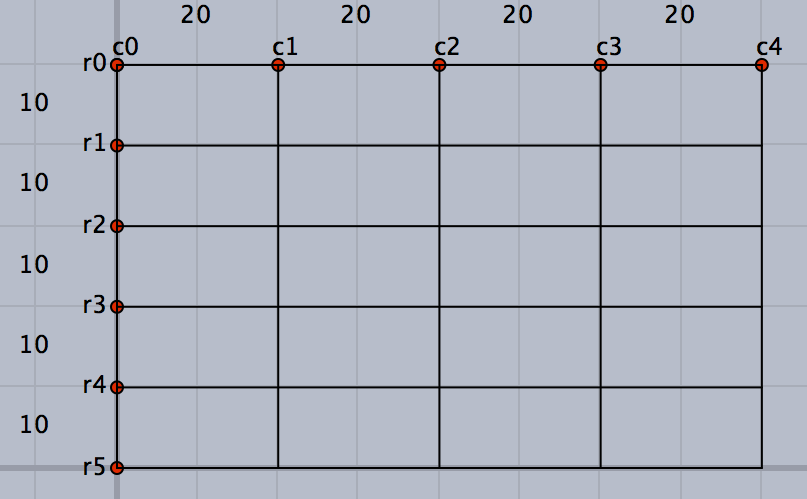
\includegraphics[bb=0 0 807 499 , width=6cm]{Fig/table01.png} → 
%%% test.tex 2014-11-24 21:36
%%% test.sce 2014-11-24 21:36
{\unitlength=6mm%
\begin{picture}%
(   8.00000,   5.00000)(   0.00000,   0.00000)%
\special{pn 8}%
%
\special{pa 0 -1181}\special{pa 472 -1181}%
\special{fp}%
\special{pa 472 -1181}\special{pa 945 -1181}%
\special{fp}%
\special{pa 945 -1181}\special{pa 1417 -1181}%
\special{fp}%
\special{pa 1417 -1181}\special{pa 1890 -1181}%
\special{fp}%
\special{pa 0 -945}\special{pa 472 -945}%
\special{fp}%
\special{pa 472 -945}\special{pa 945 -945}%
\special{fp}%
\special{pa 945 -945}\special{pa 1417 -945}%
\special{fp}%
\special{pa 1417 -945}\special{pa 1890 -945}%
\special{fp}%
\special{pa 0 -709}\special{pa 472 -709}%
\special{fp}%
\special{pa 472 -709}\special{pa 945 -709}%
\special{fp}%
\special{pa 945 -709}\special{pa 1417 -709}%
\special{fp}%
\special{pa 1417 -709}\special{pa 1890 -709}%
\special{fp}%
\special{pa 0 -472}\special{pa 472 -472}%
\special{fp}%
\special{pa 472 -472}\special{pa 945 -472}%
\special{fp}%
\special{pa 945 -472}\special{pa 1417 -472}%
\special{fp}%
\special{pa 1417 -472}\special{pa 1890 -472}%
\special{fp}%
\special{pa 0 -236}\special{pa 472 -236}%
\special{fp}%
\special{pa 472 -236}\special{pa 945 -236}%
\special{fp}%
\special{pa 945 -236}\special{pa 1417 -236}%
\special{fp}%
\special{pa 1417 -236}\special{pa 1890 -236}%
\special{fp}%
\special{pa 0 0}\special{pa 472 0}%
\special{fp}%
\special{pa 472 0}\special{pa 945 0}%
\special{fp}%
\special{pa 945 0}\special{pa 1417 0}%
\special{fp}%
\special{pa 1417 0}\special{pa 1890 0}%
\special{fp}%
\special{pa 0 -1181}\special{pa 0 -945}%
\special{fp}%
\special{pa 0 -945}\special{pa 0 -709}%
\special{fp}%
\special{pa 0 -709}\special{pa 0 -472}%
\special{fp}%
\special{pa 0 -472}\special{pa 0 -236}%
\special{fp}%
\special{pa 0 -236}\special{pa 0 0}%
\special{fp}%
\special{pa 472 -1181}\special{pa 472 -945}%
\special{fp}%
\special{pa 472 -945}\special{pa 472 -709}%
\special{fp}%
\special{pa 472 -709}\special{pa 472 -472}%
\special{fp}%
\special{pa 472 -472}\special{pa 472 -236}%
\special{fp}%
\special{pa 472 -236}\special{pa 472 0}%
\special{fp}%
\special{pa 945 -1181}\special{pa 945 -945}%
\special{fp}%
\special{pa 945 -945}\special{pa 945 -709}%
\special{fp}%
\special{pa 945 -709}\special{pa 945 -472}%
\special{fp}%
\special{pa 945 -472}\special{pa 945 -236}%
\special{fp}%
\special{pa 945 -236}\special{pa 945 0}%
\special{fp}%
\special{pa 1417 -1181}\special{pa 1417 -945}%
\special{fp}%
\special{pa 1417 -945}\special{pa 1417 -709}%
\special{fp}%
\special{pa 1417 -709}\special{pa 1417 -472}%
\special{fp}%
\special{pa 1417 -472}\special{pa 1417 -236}%
\special{fp}%
\special{pa 1417 -236}\special{pa 1417 0}%
\special{fp}%
\special{pa 1890 -1181}\special{pa 1890 -945}%
\special{fp}%
\special{pa 1890 -945}\special{pa 1890 -709}%
\special{fp}%
\special{pa 1890 -709}\special{pa 1890 -472}%
\special{fp}%
\special{pa 1890 -472}\special{pa 1890 -236}%
\special{fp}%
\special{pa 1890 -236}\special{pa 1890 0}%
\special{fp}%
\end{picture}}%\\

 表のサイズ,行幅,列幅は,作成後にそれぞれの制御点をドラッグすることにより任意に変えることができる。\\

 除外線は,除外するセルの罫線を,rとc で位置指定する。\\
  横罫線の場合,横罫線の番号,範囲(から,まで)\\
  縦罫線の場合,縦罫線の番号,範囲(から,まで)\\
とする。\\

 例:\verb|Rmv=["r1c0c1","c3r0r1","c3r3r5","r4c2c4"];|\\
   \verb|Tabledata("",4,5,80,50,Rmv);|\\
 で,次の表ができる。\\
 \\
     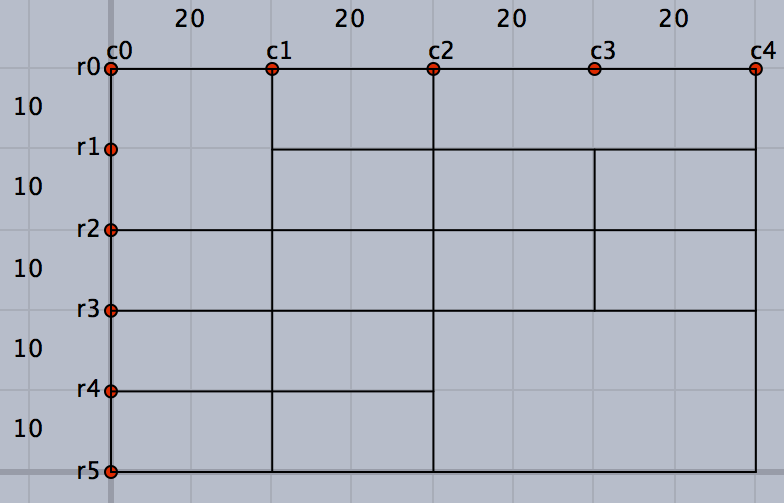
\includegraphics[bb=0 0 784 503 , width=6cm]{Fig/table03.png}\\
 除外する罫線がない場合は,空リストとする。\\

 例:\verb|Tabledata("",Yoko,Tate,[]);|\\
\\
 Tabledata()関数は,制御点r0,r1,・・・,c0,c1,・・・ がなければ新しく作り,すでに存在する場合はそのままとする。したがって,一度表を作成したのち,行数・列数を修正して作り直す場合は,一度既存の点を消去する必要がある。そのためには,「すべての点を選択する」ツールをクリックして点を消去するのがよい。クリックすると,消去後すぐに新規作成される。\\
 すでに他の点を描画してしまった場合は,表示メニューの「式による表示」で一覧表を出して,制御点を選択して消去する。\\
 ただし,行数,列数が多すぎた場合は,必ずしも作り直す必要はない。Settable() 関数により,実際に書き出す表の範囲を指定できるからである。\\

 なお,表を作成したときは,表の範囲が出力範囲として優先される(Tabledata()を実行したとき)ので,表外に図を描いた場合は,最後にこの関数で出力範囲を指定して書き出す。\\

\begin{flushright} \hyperlink{functionlist}{$\Rightarrow$関数一覧}\end{flushright}

\hypertarget{tabledatalight}{}
\item[関数] Tabledatalight(name , 縦横データ, 除外線 , options)
\item[機能] 幾何点を持たない表の枠を作成し,表のデータlist を返す
\item[説明] Tabledata()がCinderellaの幾何点を生成するのに対し,こちらは幾何点を生成しない。\\
 幾何点を作成しないメリットは,スクリプトだけで縦横幅を変更できること。デメリットはインタラクティブな微調整ができないこと。\\
 optionとして,ラベルのスキップ値(スキップするところは表示されない)を指定することができる。ただし,ラベルはCinderellaの画面上だけの問題。\\
 \\
 例: \verb|Yoko=[20,20,20,20];|\\
   \verb|Tate=[10,10,10,10,10];|\\
   \verb|Tabledatalight("",Yoko,Tate,[],[2]);|\\
 とすると,r1,r3,c1,c2 が非表示となる。\\


\begin{flushright} \hyperlink{functionlist}{$\Rightarrow$関数一覧}\end{flushright}

\hypertarget{tableseg}{}
\item[関数] Tableseg( 罫線リスト, 線種)
\item[機能] 罫線の線種を指定する
\item[説明] 罫線リストを与えて線種を指定する\\
 罫線リストは,["r1c0c1","r4c2c4"] のように与える。\\
 破線・点線にする場合は,Tabledata()であらかじめ除外しておく。\\

 例: \verb|Rmv=["r1c0c1","c3r0r1","c3r3r5","r4c2c4"];|\\
   \verb|Tabledata("",4,5,80,50,Rmv);|\\
   \verb|Tableseg(["r1c0c1","r4c2c4"],["da"]);|\\

     %%% test.tex 2014-11-26 11:41
%%% test.sce 2014-11-26 11:41
{\unitlength=6mm%
\begin{picture}%
(   8.00000,   5.00000)(   0.00000,   0.00000)%
\special{pn 8}%
%
\special{pa 0 -945}\special{pa 36 -945}\special{fp}\special{pa 73 -945}\special{pa 109 -945}\special{fp}%
\special{pa 145 -945}\special{pa 182 -945}\special{fp}\special{pa 218 -945}\special{pa 254 -945}\special{fp}%
\special{pa 291 -945}\special{pa 327 -945}\special{fp}\special{pa 363 -945}\special{pa 400 -945}\special{fp}%
\special{pa 436 -945}\special{pa 472 -945}\special{fp}%
%
\special{pa 945 -236}\special{pa 983 -236}\special{fp}\special{pa 1020 -236}\special{pa 1058 -236}\special{fp}%
\special{pa 1096 -236}\special{pa 1134 -236}\special{fp}\special{pa 1172 -236}\special{pa 1209 -236}\special{fp}%
\special{pa 1247 -236}\special{pa 1285 -236}\special{fp}\special{pa 1323 -236}\special{pa 1361 -236}\special{fp}%
\special{pa 1398 -236}\special{pa 1436 -236}\special{fp}\special{pa 1474 -236}\special{pa 1512 -236}\special{fp}%
\special{pa 1550 -236}\special{pa 1587 -236}\special{fp}\special{pa 1625 -236}\special{pa 1663 -236}\special{fp}%
\special{pa 1701 -236}\special{pa 1739 -236}\special{fp}\special{pa 1776 -236}\special{pa 1814 -236}\special{fp}%
\special{pa 1852 -236}\special{pa 1890 -236}\special{fp}%
%
\settowidth{\Width}{R0}\setlength{\Width}{-1\Width}%
\settoheight{\Height}{R0}\settodepth{\Depth}{R0}\setlength{\Height}{-0.5\Height}\setlength{\Depth}{0.5\Depth}\addtolength{\Height}{\Depth}%
\put(-0.1500,5.0000){\hspace*{\Width}\raisebox{\Height}{R0}}%
%
%
\settowidth{\Width}{R1}\setlength{\Width}{-1\Width}%
\settoheight{\Height}{R1}\settodepth{\Depth}{R1}\setlength{\Height}{-0.5\Height}\setlength{\Depth}{0.5\Depth}\addtolength{\Height}{\Depth}%
\put(-0.1500,4.0000){\hspace*{\Width}\raisebox{\Height}{R1}}%
%
%
\settowidth{\Width}{R2}\setlength{\Width}{-1\Width}%
\settoheight{\Height}{R2}\settodepth{\Depth}{R2}\setlength{\Height}{-0.5\Height}\setlength{\Depth}{0.5\Depth}\addtolength{\Height}{\Depth}%
\put(-0.1500,3.0000){\hspace*{\Width}\raisebox{\Height}{R2}}%
%
%
\settowidth{\Width}{R3}\setlength{\Width}{-1\Width}%
\settoheight{\Height}{R3}\settodepth{\Depth}{R3}\setlength{\Height}{-0.5\Height}\setlength{\Depth}{0.5\Depth}\addtolength{\Height}{\Depth}%
\put(-0.1500,2.0000){\hspace*{\Width}\raisebox{\Height}{R3}}%
%
%
\settowidth{\Width}{R4}\setlength{\Width}{-1\Width}%
\settoheight{\Height}{R4}\settodepth{\Depth}{R4}\setlength{\Height}{-0.5\Height}\setlength{\Depth}{0.5\Depth}\addtolength{\Height}{\Depth}%
\put(-0.1500,1.0000){\hspace*{\Width}\raisebox{\Height}{R4}}%
%
%
\settowidth{\Width}{R5}\setlength{\Width}{-1\Width}%
\settoheight{\Height}{R5}\settodepth{\Depth}{R5}\setlength{\Height}{-0.5\Height}\setlength{\Depth}{0.5\Depth}\addtolength{\Height}{\Depth}%
\put(-0.1500,0.0000){\hspace*{\Width}\raisebox{\Height}{R5}}%
%
%
\settowidth{\Width}{C0}\setlength{\Width}{-0.5\Width}%
\settoheight{\Height}{C0}\settodepth{\Depth}{C0}\setlength{\Height}{-\Height}%
\put(0.0000,-0.1500){\hspace*{\Width}\raisebox{\Height}{C0}}%
%
%
\settowidth{\Width}{C1}\setlength{\Width}{-0.5\Width}%
\settoheight{\Height}{C1}\settodepth{\Depth}{C1}\setlength{\Height}{-\Height}%
\put(2.0000,-0.1500){\hspace*{\Width}\raisebox{\Height}{C1}}%
%
%
\settowidth{\Width}{C2}\setlength{\Width}{-0.5\Width}%
\settoheight{\Height}{C2}\settodepth{\Depth}{C2}\setlength{\Height}{-\Height}%
\put(4.0000,-0.1500){\hspace*{\Width}\raisebox{\Height}{C2}}%
%
%
\settowidth{\Width}{C3}\setlength{\Width}{-0.5\Width}%
\settoheight{\Height}{C3}\settodepth{\Depth}{C3}\setlength{\Height}{-\Height}%
\put(6.0000,-0.1500){\hspace*{\Width}\raisebox{\Height}{C3}}%
%
%
\settowidth{\Width}{C4}\setlength{\Width}{-0.5\Width}%
\settoheight{\Height}{C4}\settodepth{\Depth}{C4}\setlength{\Height}{-\Height}%
\put(8.0000,-0.1500){\hspace*{\Width}\raisebox{\Height}{C4}}%
%
%
\special{pa 0 -1181}\special{pa 472 -1181}%
\special{fp}%
\special{pa 472 -1181}\special{pa 945 -1181}%
\special{fp}%
\special{pa 945 -1181}\special{pa 1417 -1181}%
\special{fp}%
\special{pa 1417 -1181}\special{pa 1890 -1181}%
\special{fp}%
\special{pa 472 -945}\special{pa 945 -945}%
\special{fp}%
\special{pa 945 -945}\special{pa 1417 -945}%
\special{fp}%
\special{pa 1417 -945}\special{pa 1890 -945}%
\special{fp}%
\special{pa 0 -709}\special{pa 472 -709}%
\special{fp}%
\special{pa 472 -709}\special{pa 945 -709}%
\special{fp}%
\special{pa 945 -709}\special{pa 1417 -709}%
\special{fp}%
\special{pa 1417 -709}\special{pa 1890 -709}%
\special{fp}%
\special{pa 0 -472}\special{pa 472 -472}%
\special{fp}%
\special{pa 472 -472}\special{pa 945 -472}%
\special{fp}%
\special{pa 945 -472}\special{pa 1417 -472}%
\special{fp}%
\special{pa 1417 -472}\special{pa 1890 -472}%
\special{fp}%
\special{pa 0 -236}\special{pa 472 -236}%
\special{fp}%
\special{pa 472 -236}\special{pa 945 -236}%
\special{fp}%
\special{pa 0 0}\special{pa 472 0}%
\special{fp}%
\special{pa 472 0}\special{pa 945 0}%
\special{fp}%
\special{pa 945 0}\special{pa 1417 0}%
\special{fp}%
\special{pa 1417 0}\special{pa 1890 0}%
\special{fp}%
\special{pa 0 -1181}\special{pa 0 -945}%
\special{fp}%
\special{pa 0 -945}\special{pa 0 -709}%
\special{fp}%
\special{pa 0 -709}\special{pa 0 -472}%
\special{fp}%
\special{pa 0 -472}\special{pa 0 -236}%
\special{fp}%
\special{pa 0 -236}\special{pa 0 0}%
\special{fp}%
\special{pa 472 -1181}\special{pa 472 -945}%
\special{fp}%
\special{pa 472 -945}\special{pa 472 -709}%
\special{fp}%
\special{pa 472 -709}\special{pa 472 -472}%
\special{fp}%
\special{pa 472 -472}\special{pa 472 -236}%
\special{fp}%
\special{pa 472 -236}\special{pa 472 0}%
\special{fp}%
\special{pa 945 -1181}\special{pa 945 -945}%
\special{fp}%
\special{pa 945 -945}\special{pa 945 -709}%
\special{fp}%
\special{pa 945 -709}\special{pa 945 -472}%
\special{fp}%
\special{pa 945 -472}\special{pa 945 -236}%
\special{fp}%
\special{pa 945 -236}\special{pa 945 0}%
\special{fp}%
\special{pa 1417 -945}\special{pa 1417 -709}%
\special{fp}%
\special{pa 1417 -709}\special{pa 1417 -472}%
\special{fp}%
\special{pa 1890 -1181}\special{pa 1890 -945}%
\special{fp}%
\special{pa 1890 -945}\special{pa 1890 -709}%
\special{fp}%
\special{pa 1890 -709}\special{pa 1890 -472}%
\special{fp}%
\special{pa 1890 -472}\special{pa 1890 -236}%
\special{fp}%
\special{pa 1890 -236}\special{pa 1890 0}%
\special{fp}%
\end{picture}}%\\

 注)R0,C0,・・は実際には表示されない\\
 \\
\hypertarget{changetablestyle}{}
\item[関数] ChangeTablestyle(罫線リスト, 変更オプション)
\item[機能] Table の罫線の描画オプションを変更
\item[説明] 罫線を部分的に指定して描画オプションを変更できる。\\
 \\
例:\verb|ChangeTablestyle(["r0c0c3"],["da"]);| 
 \\
 \\
\hypertarget{findcell}{}
\item[関数] Findcell(列番号, 行番号)
\item[機能] セルの情報list(中心,横幅/2,縦幅/2)を返す
\item[説明] 列番号,行番号は左上のセルを1列1行として数える。 \\

例:\verb|Tabledata(4,5,80,50,[]);|\\
  \verb|println(Findcell(tb,2,1));|\\
  とすると,2列1行のセルの中心の座標と横幅の半分,縦幅の半分の値がリストとしてコンソールに表示される。結果は [[3,4.5],1,0.5]\\ 

\begin{flushright} \hyperlink{functionlist}{$\Rightarrow$関数一覧}\end{flushright}

\hypertarget{putcell}{}
\item[関数] Putcell (列番号, 行番号, 位置, 文字データ)
\item[機能] セルに文字列を入れる
\item[説明] 複数のセルにまたぐ位置指定の場合,列番号,行番号は,セル左上と右下の制御点の名称で指定する。\\
 位置は c, r, l, t, b (中央center , 右right , 左left , 上top , 下bottom   )\\
 位置の例を以下に示す。
\begin{verbatim}
  Tabledata("",5,2,100,40,["c1r1r2","c4r1r2"]);
  Putcell(1,1,"c","A");
  Putcell(2,1,"r","B");
  Putcell(3,1,"l","C");
  Putcell(4,1,"t","D");
  Putcell(5,1,"b","E");
  Putcell(c0r1,c2r2,"c","F");
  Putcell(c2r1,c3r2,"lb","G");
  Putcell(c3r1,c5r2,"rt","H");
\end{verbatim}
 \\
   %%% test.tex 2014-11-25 22:19
%%% test.sce 2014-11-25 22:19
{\unitlength=6mm%
\begin{picture}%
(  10.00000,   4.00000)(   0.00000,   0.00000)%
\special{pn 8}%
%
\settowidth{\Width}{A}\setlength{\Width}{-0.5\Width}%
\settoheight{\Height}{A}\settodepth{\Depth}{A}\setlength{\Height}{-0.5\Height}\setlength{\Depth}{0.5\Depth}\addtolength{\Height}{\Depth}%
\put(1.0000,3.0000){\hspace*{\Width}\raisebox{\Height}{A}}%
%
%
\settowidth{\Width}{B}\setlength{\Width}{-1\Width}%
\settoheight{\Height}{B}\settodepth{\Depth}{B}\setlength{\Height}{-0.5\Height}\setlength{\Depth}{0.5\Depth}\addtolength{\Height}{\Depth}%
\put(3.9500,3.0000){\hspace*{\Width}\raisebox{\Height}{B}}%
%
%
\settowidth{\Width}{C}\setlength{\Width}{0\Width}%
\settoheight{\Height}{C}\settodepth{\Depth}{C}\setlength{\Height}{-0.5\Height}\setlength{\Depth}{0.5\Depth}\addtolength{\Height}{\Depth}%
\put(4.0500,3.0000){\hspace*{\Width}\raisebox{\Height}{C}}%
%
%
\settowidth{\Width}{D}\setlength{\Width}{-0.5\Width}%
\settoheight{\Height}{D}\settodepth{\Depth}{D}\setlength{\Height}{-\Height}%
\put(7.0000,3.9500){\hspace*{\Width}\raisebox{\Height}{D}}%
%
%
\settowidth{\Width}{E}\setlength{\Width}{-0.5\Width}%
\settoheight{\Height}{E}\settodepth{\Depth}{E}\setlength{\Height}{\Depth}%
\put(9.0000,2.0500){\hspace*{\Width}\raisebox{\Height}{E}}%
%
%
\settowidth{\Width}{F}\setlength{\Width}{-0.5\Width}%
\settoheight{\Height}{F}\settodepth{\Depth}{F}\setlength{\Height}{-0.5\Height}\setlength{\Depth}{0.5\Depth}\addtolength{\Height}{\Depth}%
\put(2.0000,1.0000){\hspace*{\Width}\raisebox{\Height}{F}}%
%
%
\settowidth{\Width}{G}\setlength{\Width}{0\Width}%
\settoheight{\Height}{G}\settodepth{\Depth}{G}\setlength{\Height}{\Depth}%
\put(4.0500,0.0500){\hspace*{\Width}\raisebox{\Height}{G}}%
%
%
\settowidth{\Width}{H}\setlength{\Width}{-1\Width}%
\settoheight{\Height}{H}\settodepth{\Depth}{H}\setlength{\Height}{-\Height}%
\put(9.9500,1.9500){\hspace*{\Width}\raisebox{\Height}{H}}%
%
%
\settowidth{\Width}{R0}\setlength{\Width}{-1\Width}%
\settoheight{\Height}{R0}\settodepth{\Depth}{R0}\setlength{\Height}{-0.5\Height}\setlength{\Depth}{0.5\Depth}\addtolength{\Height}{\Depth}%
\put(-0.1500,4.0000){\hspace*{\Width}\raisebox{\Height}{R0}}%
%
%
\settowidth{\Width}{R1}\setlength{\Width}{-1\Width}%
\settoheight{\Height}{R1}\settodepth{\Depth}{R1}\setlength{\Height}{-0.5\Height}\setlength{\Depth}{0.5\Depth}\addtolength{\Height}{\Depth}%
\put(-0.1500,2.0000){\hspace*{\Width}\raisebox{\Height}{R1}}%
%
%
\settowidth{\Width}{R2}\setlength{\Width}{-1\Width}%
\settoheight{\Height}{R2}\settodepth{\Depth}{R2}\setlength{\Height}{\Depth}%
\put(-0.1500,0.0500){\hspace*{\Width}\raisebox{\Height}{R2}}%
%
%
\settowidth{\Width}{C0}\setlength{\Width}{-0.5\Width}%
\settoheight{\Height}{C0}\settodepth{\Depth}{C0}\setlength{\Height}{-\Height}%
\put(0.0000,-0.1500){\hspace*{\Width}\raisebox{\Height}{C0}}%
%
%
\settowidth{\Width}{C1}\setlength{\Width}{-0.5\Width}%
\settoheight{\Height}{C1}\settodepth{\Depth}{C1}\setlength{\Height}{-\Height}%
\put(2.0000,-0.1500){\hspace*{\Width}\raisebox{\Height}{C1}}%
%
%
\settowidth{\Width}{C2}\setlength{\Width}{-0.5\Width}%
\settoheight{\Height}{C2}\settodepth{\Depth}{C2}\setlength{\Height}{-\Height}%
\put(4.0000,-0.1500){\hspace*{\Width}\raisebox{\Height}{C2}}%
%
%
\settowidth{\Width}{C3}\setlength{\Width}{-0.5\Width}%
\settoheight{\Height}{C3}\settodepth{\Depth}{C3}\setlength{\Height}{-\Height}%
\put(6.0000,-0.1500){\hspace*{\Width}\raisebox{\Height}{C3}}%
%
%
\settowidth{\Width}{C4}\setlength{\Width}{-0.5\Width}%
\settoheight{\Height}{C4}\settodepth{\Depth}{C4}\setlength{\Height}{-\Height}%
\put(8.0000,-0.1500){\hspace*{\Width}\raisebox{\Height}{C4}}%
%
%
\settowidth{\Width}{C5}\setlength{\Width}{-0.5\Width}%
\settoheight{\Height}{C5}\settodepth{\Depth}{C5}\setlength{\Height}{-\Height}%
\put(10.0000,-0.1500){\hspace*{\Width}\raisebox{\Height}{C5}}%
%
%
\special{pa 0 -945}\special{pa 472 -945}%
\special{fp}%
\special{pa 472 -945}\special{pa 945 -945}%
\special{fp}%
\special{pa 945 -945}\special{pa 1417 -945}%
\special{fp}%
\special{pa 1417 -945}\special{pa 1890 -945}%
\special{fp}%
\special{pa 1890 -945}\special{pa 2362 -945}%
\special{fp}%
\special{pa 0 -472}\special{pa 472 -472}%
\special{fp}%
\special{pa 472 -472}\special{pa 945 -472}%
\special{fp}%
\special{pa 945 -472}\special{pa 1417 -472}%
\special{fp}%
\special{pa 1417 -472}\special{pa 1890 -472}%
\special{fp}%
\special{pa 1890 -472}\special{pa 2362 -472}%
\special{fp}%
\special{pa 0 0}\special{pa 472 0}%
\special{fp}%
\special{pa 472 0}\special{pa 945 0}%
\special{fp}%
\special{pa 945 0}\special{pa 1417 0}%
\special{fp}%
\special{pa 1417 0}\special{pa 1890 0}%
\special{fp}%
\special{pa 1890 0}\special{pa 2362 0}%
\special{fp}%
\special{pa 0 -945}\special{pa 0 -472}%
\special{fp}%
\special{pa 0 -472}\special{pa 0 0}%
\special{fp}%
\special{pa 472 -945}\special{pa 472 -472}%
\special{fp}%
\special{pa 945 -945}\special{pa 945 -472}%
\special{fp}%
\special{pa 945 -472}\special{pa 945 0}%
\special{fp}%
\special{pa 1417 -945}\special{pa 1417 -472}%
\special{fp}%
\special{pa 1417 -472}\special{pa 1417 0}%
\special{fp}%
\special{pa 1890 -945}\special{pa 1890 -472}%
\special{fp}%
\special{pa 2362 -945}\special{pa 2362 -472}%
\special{fp}%
\special{pa 2362 -472}\special{pa 2362 0}%
\special{fp}%
\end{picture}}%\\
 ※R0,C0,・・は実際には表示されない\\

\begin{flushright} \hyperlink{functionlist}{$\Rightarrow$関数一覧}\end{flushright}

\hypertarget{putcol}{}
\item[関数] PutcoL (列番号, 文字位置,文字列リスト)
\item[機能] 1列に順に文字を書き入れる
\item[説明] 列番号で指定した列に,第1行から順に文字列リストの文字を書き入れる\\
 数の場合はダブルクウォートでくくらなくてもよい。\\
 セルを飛ばす場合は,ヌル文字列 "" を書く。\\


\hypertarget{putcolexpr}{}
\item[関数] PutcoLexpr (列番号, 文字位置,文字列リスト)
\item[機能] 1列に順に文字を書き入れる
\item[説明] 文字列に\TeX 書式を使うことができる\\

\hypertarget{putrow}{}
\item[関数] Putrow (行番号, 文字位置,文字列リスト)
\item[機能] 1行に順に文字を書き入れる
\item[説明] 行番号で指定した行に,第1列から順に文字列リストの文字を書き入れる。\\


\hypertarget{putrowexpr}{}
\item[関数] Putrowexpr (行番号, 文字位置,文字列リスト)
\item[機能] 1行に順に文字を書き入れる
\item[説明] 文字列に\TeX 書式を使うことができる\\

文字を入れる例を示す。
\begin{verbatim}
  Tabledata("",5,3,100,45,["c1r1r2","r1c2c3","r2c2c3"]);
  PutcoL(3,"c",["A","B","C"]);
  PutcoLexpr(4,"l",["x^2","y=\sqrt{x^3}"]);
  Putrow(1,"c",[1,"二"]);
  Putrowexpr(3,"c",["","\frac{\pi}{2}","","","\sum{x^2}"]);
\end{verbatim}

     %%% test.tex 2014-11-26 11:26
%%% test.sce 2014-11-26 11:26
{\unitlength=6mm%
\begin{picture}%
(  10.00000,   4.50000)(   0.00000,   0.00000)%
\special{pn 8}%
%
\settowidth{\Width}{A}\setlength{\Width}{-0.5\Width}%
\settoheight{\Height}{A}\settodepth{\Depth}{A}\setlength{\Height}{-0.5\Height}\setlength{\Depth}{0.5\Depth}\addtolength{\Height}{\Depth}%
\put(5.0000,3.7500){\hspace*{\Width}\raisebox{\Height}{A}}%
%
%
\settowidth{\Width}{B}\setlength{\Width}{-0.5\Width}%
\settoheight{\Height}{B}\settodepth{\Depth}{B}\setlength{\Height}{-0.5\Height}\setlength{\Depth}{0.5\Depth}\addtolength{\Height}{\Depth}%
\put(5.0000,2.2500){\hspace*{\Width}\raisebox{\Height}{B}}%
%
%
\settowidth{\Width}{C}\setlength{\Width}{-0.5\Width}%
\settoheight{\Height}{C}\settodepth{\Depth}{C}\setlength{\Height}{-0.5\Height}\setlength{\Depth}{0.5\Depth}\addtolength{\Height}{\Depth}%
\put(5.0000,0.7500){\hspace*{\Width}\raisebox{\Height}{C}}%
%
%
\settowidth{\Width}{$x^2$}\setlength{\Width}{0\Width}%
\settoheight{\Height}{$x^2$}\settodepth{\Depth}{$x^2$}\setlength{\Height}{-0.5\Height}\setlength{\Depth}{0.5\Depth}\addtolength{\Height}{\Depth}%
\put(6.0500,3.7500){\hspace*{\Width}\raisebox{\Height}{$x^2$}}%
%
%
\settowidth{\Width}{$y=\sqrt{x^3}$}\setlength{\Width}{0\Width}%
\settoheight{\Height}{$y=\sqrt{x^3}$}\settodepth{\Depth}{$y=\sqrt{x^3}$}\setlength{\Height}{-0.5\Height}\setlength{\Depth}{0.5\Depth}\addtolength{\Height}{\Depth}%
\put(6.0500,2.2500){\hspace*{\Width}\raisebox{\Height}{$y=\sqrt{x^3}$}}%
%
%
\settowidth{\Width}{1}\setlength{\Width}{-0.5\Width}%
\settoheight{\Height}{1}\settodepth{\Depth}{1}\setlength{\Height}{-0.5\Height}\setlength{\Depth}{0.5\Depth}\addtolength{\Height}{\Depth}%
\put(1.0000,3.7500){\hspace*{\Width}\raisebox{\Height}{1}}%
%
%
\settowidth{\Width}{二}\setlength{\Width}{-0.5\Width}%
\settoheight{\Height}{二}\settodepth{\Depth}{二}\setlength{\Height}{-0.5\Height}\setlength{\Depth}{0.5\Depth}\addtolength{\Height}{\Depth}%
\put(3.0000,3.7500){\hspace*{\Width}\raisebox{\Height}{二}}%
%
%
\settowidth{\Width}{$$}\setlength{\Width}{-0.5\Width}%
\settoheight{\Height}{$$}\settodepth{\Depth}{$$}\setlength{\Height}{-0.5\Height}\setlength{\Depth}{0.5\Depth}\addtolength{\Height}{\Depth}%
\put(1.0000,0.7500){\hspace*{\Width}\raisebox{\Height}{$$}}%
%
%
\settowidth{\Width}{$\frac{\pi}{2}$}\setlength{\Width}{-0.5\Width}%
\settoheight{\Height}{$\frac{\pi}{2}$}\settodepth{\Depth}{$\frac{\pi}{2}$}\setlength{\Height}{-0.5\Height}\setlength{\Depth}{0.5\Depth}\addtolength{\Height}{\Depth}%
\put(3.0000,0.7500){\hspace*{\Width}\raisebox{\Height}{$\frac{\pi}{2}$}}%
%
%
\settowidth{\Width}{$$}\setlength{\Width}{-0.5\Width}%
\settoheight{\Height}{$$}\settodepth{\Depth}{$$}\setlength{\Height}{-0.5\Height}\setlength{\Depth}{0.5\Depth}\addtolength{\Height}{\Depth}%
\put(5.0000,0.7500){\hspace*{\Width}\raisebox{\Height}{$$}}%
%
%
\settowidth{\Width}{$$}\setlength{\Width}{-0.5\Width}%
\settoheight{\Height}{$$}\settodepth{\Depth}{$$}\setlength{\Height}{-0.5\Height}\setlength{\Depth}{0.5\Depth}\addtolength{\Height}{\Depth}%
\put(7.2000,0.7500){\hspace*{\Width}\raisebox{\Height}{$$}}%
%
%
\settowidth{\Width}{$\sum{x^2}$}\setlength{\Width}{-0.5\Width}%
\settoheight{\Height}{$\sum{x^2}$}\settodepth{\Depth}{$\sum{x^2}$}\setlength{\Height}{-0.5\Height}\setlength{\Depth}{0.5\Depth}\addtolength{\Height}{\Depth}%
\put(9.2000,0.7500){\hspace*{\Width}\raisebox{\Height}{$\sum{x^2}$}}%
%
%
\settowidth{\Width}{R0}\setlength{\Width}{-1\Width}%
\settoheight{\Height}{R0}\settodepth{\Depth}{R0}\setlength{\Height}{-0.5\Height}\setlength{\Depth}{0.5\Depth}\addtolength{\Height}{\Depth}%
\put(-0.1500,4.5000){\hspace*{\Width}\raisebox{\Height}{R0}}%
%
%
\settowidth{\Width}{R1}\setlength{\Width}{-1\Width}%
\settoheight{\Height}{R1}\settodepth{\Depth}{R1}\setlength{\Height}{-0.5\Height}\setlength{\Depth}{0.5\Depth}\addtolength{\Height}{\Depth}%
\put(-0.1500,3.0000){\hspace*{\Width}\raisebox{\Height}{R1}}%
%
%
\settowidth{\Width}{R2}\setlength{\Width}{-1\Width}%
\settoheight{\Height}{R2}\settodepth{\Depth}{R2}\setlength{\Height}{-0.5\Height}\setlength{\Depth}{0.5\Depth}\addtolength{\Height}{\Depth}%
\put(-0.1500,1.5000){\hspace*{\Width}\raisebox{\Height}{R2}}%
%
%
\settowidth{\Width}{R3}\setlength{\Width}{-1\Width}%
\settoheight{\Height}{R3}\settodepth{\Depth}{R3}\setlength{\Height}{-0.5\Height}\setlength{\Depth}{0.5\Depth}\addtolength{\Height}{\Depth}%
\put(-0.1500,0.0000){\hspace*{\Width}\raisebox{\Height}{R3}}%
%
%
\settowidth{\Width}{C0}\setlength{\Width}{-0.5\Width}%
\settoheight{\Height}{C0}\settodepth{\Depth}{C0}\setlength{\Height}{-\Height}%
\put(0.0000,-0.1500){\hspace*{\Width}\raisebox{\Height}{C0}}%
%
%
\settowidth{\Width}{C1}\setlength{\Width}{-0.5\Width}%
\settoheight{\Height}{C1}\settodepth{\Depth}{C1}\setlength{\Height}{-\Height}%
\put(2.0000,-0.1500){\hspace*{\Width}\raisebox{\Height}{C1}}%
%
%
\settowidth{\Width}{C2}\setlength{\Width}{-0.5\Width}%
\settoheight{\Height}{C2}\settodepth{\Depth}{C2}\setlength{\Height}{-\Height}%
\put(4.0000,-0.1500){\hspace*{\Width}\raisebox{\Height}{C2}}%
%
%
\settowidth{\Width}{C3}\setlength{\Width}{-0.5\Width}%
\settoheight{\Height}{C3}\settodepth{\Depth}{C3}\setlength{\Height}{-\Height}%
\put(6.0000,-0.1500){\hspace*{\Width}\raisebox{\Height}{C3}}%
%
%
\settowidth{\Width}{C4}\setlength{\Width}{-0.5\Width}%
\settoheight{\Height}{C4}\settodepth{\Depth}{C4}\setlength{\Height}{-\Height}%
\put(8.4000,-0.1500){\hspace*{\Width}\raisebox{\Height}{C4}}%
%
%
\settowidth{\Width}{C5}\setlength{\Width}{-0.5\Width}%
\settoheight{\Height}{C5}\settodepth{\Depth}{C5}\setlength{\Height}{-\Height}%
\put(10.0000,-0.1500){\hspace*{\Width}\raisebox{\Height}{C5}}%
%
%
\special{pa 0 -1063}\special{pa 472 -1063}%
\special{fp}%
\special{pa 472 -1063}\special{pa 945 -1063}%
\special{fp}%
\special{pa 945 -1063}\special{pa 1417 -1063}%
\special{fp}%
\special{pa 1417 -1063}\special{pa 1984 -1063}%
\special{fp}%
\special{pa 1984 -1063}\special{pa 2362 -1063}%
\special{fp}%
\special{pa 0 -709}\special{pa 472 -709}%
\special{fp}%
\special{pa 472 -709}\special{pa 945 -709}%
\special{fp}%
\special{pa 1417 -709}\special{pa 1984 -709}%
\special{fp}%
\special{pa 1984 -709}\special{pa 2362 -709}%
\special{fp}%
\special{pa 0 -354}\special{pa 472 -354}%
\special{fp}%
\special{pa 472 -354}\special{pa 945 -354}%
\special{fp}%
\special{pa 1417 -354}\special{pa 1984 -354}%
\special{fp}%
\special{pa 1984 -354}\special{pa 2362 -354}%
\special{fp}%
\special{pa 0 0}\special{pa 472 0}%
\special{fp}%
\special{pa 472 0}\special{pa 945 0}%
\special{fp}%
\special{pa 945 0}\special{pa 1417 0}%
\special{fp}%
\special{pa 1417 0}\special{pa 1984 0}%
\special{fp}%
\special{pa 1984 0}\special{pa 2362 0}%
\special{fp}%
\special{pa 0 -1063}\special{pa 0 -709}%
\special{fp}%
\special{pa 0 -709}\special{pa 0 -354}%
\special{fp}%
\special{pa 0 -354}\special{pa 0 0}%
\special{fp}%
\special{pa 472 -1063}\special{pa 472 -709}%
\special{fp}%
\special{pa 472 -354}\special{pa 472 0}%
\special{fp}%
\special{pa 945 -1063}\special{pa 945 -709}%
\special{fp}%
\special{pa 945 -709}\special{pa 945 -354}%
\special{fp}%
\special{pa 945 -354}\special{pa 945 0}%
\special{fp}%
\special{pa 1417 -1063}\special{pa 1417 -709}%
\special{fp}%
\special{pa 1417 -709}\special{pa 1417 -354}%
\special{fp}%
\special{pa 1417 -354}\special{pa 1417 0}%
\special{fp}%
\special{pa 1984 -1063}\special{pa 1984 -709}%
\special{fp}%
\special{pa 1984 -709}\special{pa 1984 -354}%
\special{fp}%
\special{pa 1984 -354}\special{pa 1984 0}%
\special{fp}%
\special{pa 2362 -1063}\special{pa 2362 -709}%
\special{fp}%
\special{pa 2362 -709}\special{pa 2362 -354}%
\special{fp}%
\special{pa 2362 -354}\special{pa 2362 0}%
\special{fp}%
\end{picture}}%\\

 ※ R0,C0,・・は実際には表示されない\\
  また,この例では,C4列の罫線を,制御点C4をドラッグすることにより\\
  右にずらしている。\\
\\

グラフや文を入れた表の作成例\\

 PutcoLexpr(),Putrowexpr() では,数式だけでなく,一般の\TeX の文を入れることができる。\\
 また,グラフの位置を適当に合わせて描画することにより,表のセルの中にグラフを入れることができる。\\

 例:2次関数のグラフと2次方程式の判別式の関係\\
  セルの中にグラフを描く例。実際には,セルの位置にグラフを描いているだけ。
\begin{verbatim}
  Tabledata("",3,3,120,90,["r1c0c3","r2c0c3"],["dr,2"]);
  Tableseg(["r1c0c3"],["dr"]);
  Tableseg(["r2c0c3"],["da"]);
  Plotdata("1","(x-2)^2+1.5","x=[0.5,3.5]");
  Plotdata("2","(x-6)^2+2","x=[4.5,7.5]");
  Plotdata("3","(x-10)^2+2.5","x=[8.5,11.5]");
  Listplot([A,B]);
  Listplot([C,D]);
  Listplot([E,F]);
  Putrowexpr(1,"c",["D>0","D=0","D<0"]);
  Putrow(2,"c",["2点で交わる","接する","共有点なし"]);
  Letter(G,"c","判別式と$x$軸の交点");
\end{verbatim}
 \\
       %%% fig.tex 2014-12-18 15:16
%%% fig.sce 2014-12-18 15:16
{\unitlength=5mm%
\begin{picture}%
(  12.00000,   9.00000)(  -0.00000,  -0.00000)%
\special{pn 8}%
%
\special{pn 16}%
\special{pa 0 -1772}\special{pa 787 -1772}%
\special{fp}%
\special{pn 8}%
\special{pn 16}%
\special{pa 787 -1772}\special{pa 1575 -1772}%
\special{fp}%
\special{pn 8}%
\special{pn 16}%
\special{pa 1575 -1772}\special{pa 2362 -1772}%
\special{fp}%
\special{pn 8}%
\special{pn 16}%
\special{pa 0 0}\special{pa 787 0}%
\special{fp}%
\special{pn 8}%
\special{pn 16}%
\special{pa 787 0}\special{pa 1575 0}%
\special{fp}%
\special{pn 8}%
\special{pn 16}%
\special{pa 1575 0}\special{pa 2362 0}%
\special{fp}%
\special{pn 8}%
\special{pn 16}%
\special{pa 0 -1772}\special{pa 0 -1378}%
\special{fp}%
\special{pn 8}%
\special{pn 16}%
\special{pa 0 -1378}\special{pa 0 -1102}%
\special{fp}%
\special{pn 8}%
\special{pn 16}%
\special{pa 0 -1102}\special{pa 0 0}%
\special{fp}%
\special{pn 8}%
\special{pn 16}%
\special{pa 787 -1772}\special{pa 787 -1378}%
\special{fp}%
\special{pn 8}%
\special{pn 16}%
\special{pa 787 -1378}\special{pa 787 -1102}%
\special{fp}%
\special{pn 8}%
\special{pn 16}%
\special{pa 787 -1102}\special{pa 787 0}%
\special{fp}%
\special{pn 8}%
\special{pn 16}%
\special{pa 1575 -1772}\special{pa 1575 -1378}%
\special{fp}%
\special{pn 8}%
\special{pn 16}%
\special{pa 1575 -1378}\special{pa 1575 -1102}%
\special{fp}%
\special{pn 8}%
\special{pn 16}%
\special{pa 1575 -1102}\special{pa 1575 0}%
\special{fp}%
\special{pn 8}%
\special{pn 16}%
\special{pa 2362 -1772}\special{pa 2362 -1378}%
\special{fp}%
\special{pn 8}%
\special{pn 16}%
\special{pa 2362 -1378}\special{pa 2362 -1102}%
\special{fp}%
\special{pn 8}%
\special{pn 16}%
\special{pa 2362 -1102}\special{pa 2362 0}%
\special{fp}%
\special{pn 8}%
\special{pa 0 -1378}\special{pa 2362 -1378}%
\special{fp}%
\special{pa 0 -1102}\special{pa 39 -1102}\special{fp}\special{pa 77 -1102}\special{pa 116 -1102}\special{fp}%
\special{pa 155 -1102}\special{pa 194 -1102}\special{fp}\special{pa 232 -1102}\special{pa 271 -1102}\special{fp}%
\special{pa 310 -1102}\special{pa 349 -1102}\special{fp}\special{pa 387 -1102}\special{pa 426 -1102}\special{fp}%
\special{pa 465 -1102}\special{pa 503 -1102}\special{fp}\special{pa 542 -1102}\special{pa 581 -1102}\special{fp}%
\special{pa 620 -1102}\special{pa 658 -1102}\special{fp}\special{pa 697 -1102}\special{pa 736 -1102}\special{fp}%
\special{pa 774 -1102}\special{pa 813 -1102}\special{fp}\special{pa 852 -1102}\special{pa 891 -1102}\special{fp}%
\special{pa 929 -1102}\special{pa 968 -1102}\special{fp}\special{pa 1007 -1102}\special{pa 1046 -1102}\special{fp}%
\special{pa 1084 -1102}\special{pa 1123 -1102}\special{fp}\special{pa 1162 -1102}\special{pa 1200 -1102}\special{fp}%
\special{pa 1239 -1102}\special{pa 1278 -1102}\special{fp}\special{pa 1317 -1102}\special{pa 1355 -1102}\special{fp}%
\special{pa 1394 -1102}\special{pa 1433 -1102}\special{fp}\special{pa 1472 -1102}\special{pa 1510 -1102}\special{fp}%
\special{pa 1549 -1102}\special{pa 1588 -1102}\special{fp}\special{pa 1626 -1102}\special{pa 1665 -1102}\special{fp}%
\special{pa 1704 -1102}\special{pa 1743 -1102}\special{fp}\special{pa 1781 -1102}\special{pa 1820 -1102}\special{fp}%
\special{pa 1859 -1102}\special{pa 1898 -1102}\special{fp}\special{pa 1936 -1102}\special{pa 1975 -1102}\special{fp}%
\special{pa 2014 -1102}\special{pa 2052 -1102}\special{fp}\special{pa 2091 -1102}\special{pa 2130 -1102}\special{fp}%
\special{pa 2169 -1102}\special{pa 2207 -1102}\special{fp}\special{pa 2246 -1102}\special{pa 2285 -1102}\special{fp}%
\special{pa 2323 -1102}\special{pa 2362 -1102}\special{fp}%
%
\settowidth{\Width}{$D>0$}\setlength{\Width}{-0.5\Width}%
\settoheight{\Height}{$D>0$}\settodepth{\Depth}{$D>0$}\setlength{\Height}{-0.5\Height}\setlength{\Depth}{0.5\Depth}\addtolength{\Height}{\Depth}%
\put(2.0000,8.0000){\hspace*{\Width}\raisebox{\Height}{$D>0$}}%
%
%
\settowidth{\Width}{$D=0$}\setlength{\Width}{-0.5\Width}%
\settoheight{\Height}{$D=0$}\settodepth{\Depth}{$D=0$}\setlength{\Height}{-0.5\Height}\setlength{\Depth}{0.5\Depth}\addtolength{\Height}{\Depth}%
\put(6.0000,8.0000){\hspace*{\Width}\raisebox{\Height}{$D=0$}}%
%
%
\settowidth{\Width}{$D<0$}\setlength{\Width}{-0.5\Width}%
\settoheight{\Height}{$D<0$}\settodepth{\Depth}{$D<0$}\setlength{\Height}{-0.5\Height}\setlength{\Depth}{0.5\Depth}\addtolength{\Height}{\Depth}%
\put(10.0000,8.0000){\hspace*{\Width}\raisebox{\Height}{$D<0$}}%
%
%
\settowidth{\Width}{2点で交わる}\setlength{\Width}{-0.5\Width}%
\settoheight{\Height}{2点で交わる}\settodepth{\Depth}{2点で交わる}\setlength{\Height}{-0.5\Height}\setlength{\Depth}{0.5\Depth}\addtolength{\Height}{\Depth}%
\put(2.0000,6.3000){\hspace*{\Width}\raisebox{\Height}{2点で交わる}}%
%
%
\settowidth{\Width}{接する}\setlength{\Width}{-0.5\Width}%
\settoheight{\Height}{接する}\settodepth{\Depth}{接する}\setlength{\Height}{-0.5\Height}\setlength{\Depth}{0.5\Depth}\addtolength{\Height}{\Depth}%
\put(6.0000,6.3000){\hspace*{\Width}\raisebox{\Height}{接する}}%
%
%
\settowidth{\Width}{共有点なし}\setlength{\Width}{-0.5\Width}%
\settoheight{\Height}{共有点なし}\settodepth{\Depth}{共有点なし}\setlength{\Height}{-0.5\Height}\setlength{\Depth}{0.5\Depth}\addtolength{\Height}{\Depth}%
\put(10.0000,6.3000){\hspace*{\Width}\raisebox{\Height}{共有点なし}}%
%
%
\settowidth{\Width}{判別式と$x$軸の交点}\setlength{\Width}{-0.5\Width}%
\settoheight{\Height}{判別式と$x$軸の交点}\settodepth{\Depth}{判別式と$x$軸の交点}\setlength{\Height}{-0.5\Height}\setlength{\Depth}{0.5\Depth}\addtolength{\Height}{\Depth}%
\put(4.0000,10.0000){\hspace*{\Width}\raisebox{\Height}{判別式と$x$軸の交点}}%
%
%
\special{pa 98 -738}\special{pa 110 -703}\special{pa 123 -669}\special{pa 135 -636}%
\special{pa 147 -605}\special{pa 159 -576}\special{pa 171 -548}\special{pa 183 -521}%
\special{pa 195 -496}\special{pa 207 -473}\special{pa 219 -450}\special{pa 231 -430}%
\special{pa 243 -411}\special{pa 255 -393}\special{pa 267 -377}\special{pa 279 -362}%
\special{pa 291 -349}\special{pa 303 -337}\special{pa 315 -326}\special{pa 327 -318}%
\special{pa 339 -310}\special{pa 352 -304}\special{pa 364 -300}\special{pa 376 -297}%
\special{pa 388 -295}\special{pa 400 -295}\special{pa 412 -297}\special{pa 424 -300}%
\special{pa 436 -304}\special{pa 448 -310}\special{pa 460 -318}\special{pa 472 -326}%
\special{pa 484 -337}\special{pa 496 -349}\special{pa 508 -362}\special{pa 520 -377}%
\special{pa 532 -393}\special{pa 544 -411}\special{pa 556 -430}\special{pa 568 -450}%
\special{pa 581 -473}\special{pa 593 -496}\special{pa 605 -521}\special{pa 617 -548}%
\special{pa 629 -576}\special{pa 641 -605}\special{pa 653 -636}\special{pa 665 -669}%
\special{pa 677 -703}\special{pa 689 -738}%
\special{fp}%
\special{pa 886 -837}\special{pa 898 -801}\special{pa 910 -767}\special{pa 922 -735}%
\special{pa 934 -704}\special{pa 946 -674}\special{pa 958 -646}\special{pa 970 -620}%
\special{pa 982 -595}\special{pa 994 -571}\special{pa 1006 -549}\special{pa 1018 -528}%
\special{pa 1030 -509}\special{pa 1043 -491}\special{pa 1055 -475}\special{pa 1067 -460}%
\special{pa 1079 -447}\special{pa 1091 -435}\special{pa 1103 -425}\special{pa 1115 -416}%
\special{pa 1127 -409}\special{pa 1139 -403}\special{pa 1151 -398}\special{pa 1163 -395}%
\special{pa 1175 -394}\special{pa 1187 -394}\special{pa 1199 -395}\special{pa 1211 -398}%
\special{pa 1223 -403}\special{pa 1235 -409}\special{pa 1247 -416}\special{pa 1259 -425}%
\special{pa 1271 -435}\special{pa 1284 -447}\special{pa 1296 -460}\special{pa 1308 -475}%
\special{pa 1320 -491}\special{pa 1332 -509}\special{pa 1344 -528}\special{pa 1356 -549}%
\special{pa 1368 -571}\special{pa 1380 -595}\special{pa 1392 -620}\special{pa 1404 -646}%
\special{pa 1416 -674}\special{pa 1428 -704}\special{pa 1440 -735}\special{pa 1452 -767}%
\special{pa 1464 -801}\special{pa 1476 -837}%
\special{fp}%
\special{pa 1673 -935}\special{pa 1685 -900}\special{pa 1697 -866}\special{pa 1709 -833}%
\special{pa 1721 -802}\special{pa 1733 -773}\special{pa 1746 -745}\special{pa 1758 -718}%
\special{pa 1770 -693}\special{pa 1782 -669}\special{pa 1794 -647}\special{pa 1806 -627}%
\special{pa 1818 -607}\special{pa 1830 -590}\special{pa 1842 -573}\special{pa 1854 -559}%
\special{pa 1866 -545}\special{pa 1878 -534}\special{pa 1890 -523}\special{pa 1902 -514}%
\special{pa 1914 -507}\special{pa 1926 -501}\special{pa 1938 -497}\special{pa 1950 -494}%
\special{pa 1962 -492}\special{pa 1975 -492}\special{pa 1987 -494}\special{pa 1999 -497}%
\special{pa 2011 -501}\special{pa 2023 -507}\special{pa 2035 -514}\special{pa 2047 -523}%
\special{pa 2059 -534}\special{pa 2071 -545}\special{pa 2083 -559}\special{pa 2095 -573}%
\special{pa 2107 -590}\special{pa 2119 -607}\special{pa 2131 -627}\special{pa 2143 -647}%
\special{pa 2155 -669}\special{pa 2167 -693}\special{pa 2179 -718}\special{pa 2191 -745}%
\special{pa 2204 -773}\special{pa 2216 -802}\special{pa 2228 -833}\special{pa 2240 -866}%
\special{pa 2252 -900}\special{pa 2264 -935}%
\special{fp}%
\special{pa 197 -394}\special{pa 591 -394}%
\special{fp}%
\special{pa 984 -394}\special{pa 1378 -394}%
\special{fp}%
\special{pa 1772 -394}\special{pa 2165 -394}%
\special{fp}%
\end{picture}}%\\
\\
注意:この例を実行するとわかるが,セルのサイズと文字サイズの関係などにより,Cinderellaの画面上と\TeX への書き出しは必ずしも同一にはならない。\\

\newpage
 例:増減表とグラフ\\

 関数の増減表とグラフを1つの表の中に入れた例。
\begin{verbatim}
  Tate=[6,6,10,6,10,6,40];
  Yoko=[30,6,6,6];
  Rmv=["c1r0r1","c2r0r1","c3r0r1","c4r0r1","c5r0r1", "r1c6c7","r2c6c7","r3c6c7"];
  Tabledata("",Tate,Yoko,Rmv,["dr"]);
  Tlistplot("23d",["c1r2","c2r3"]);
  Tlistplot("23u",["c1r3","c2r2"]);
  Putrowexpr(2,"c",["x",0,"\cdots","\tfrac{1}{4}","\cdots",4]);
  Putrowexpr(3,"c",["y`","","-",0,"+"]);
  Putrowexpr(4,"c",["y",0,"\searrow","-\tfrac{1}{4}","\nearrow",2]);
  Putcell(1,1,"l2t2","{\small\begin{minipage}{44mm}$y=x-\sqrt{x}$\\$y`=
  \dfrac{2\sqrt{x}-1}{2\sqrt{x}}=0$|より\vspace{1mm}\\\hspace*{2zw}$x=
  \dfrac{1}{4}$\vspace{1mm}\\増減表は次のようになる\end{minipage}}" );
  Plotdata("1","x-sqrt(x)","x=[0,3]",["do","notex"]);
  Listplot("2",[[0,0],[3,0]],["do","notex"]);
  Listplot("3",[[0,-0.5],[0,3]],["do","notex"]);
  Translatedata("1","gr1",[4.9,1],["dr"]);
  Translatedata("2","sg2",[4.9,1],["dr"]);
  Translatedata("3","sg3",[4.9,1],["dr"]);
  Letter(Ptend(tr2),"e1","\small{$x$}");
  Letter(Ptend(tr3),"n1","\small{$y$}");
  Letter(Ptstart(tr2),"w1","\small O");
  Expr(Ptend(tr1),"nw-2","y=x-\sqrt{x}");
\end{verbatim}
       %%% test.tex 2014-11-26 12:54
%%% test.sce 2014-11-26 12:54
{\unitlength=1cm%
\begin{picture}%
(   8.50000,   5.00000)(   0.00000,   0.00000)%
\special{pn 8}%
%
\special{pa 0 -1969}\special{pa 236 -1969}%
\special{fp}%
\special{pa 236 -1969}\special{pa 472 -1969}%
\special{fp}%
\special{pa 472 -1969}\special{pa 866 -1969}%
\special{fp}%
\special{pa 866 -1969}\special{pa 1102 -1969}%
\special{fp}%
\special{pa 1102 -1969}\special{pa 1496 -1969}%
\special{fp}%
\special{pa 1496 -1969}\special{pa 1732 -1969}%
\special{fp}%
\special{pa 1732 -1969}\special{pa 3346 -1969}%
\special{fp}%
\special{pa 0 -709}\special{pa 236 -709}%
\special{fp}%
\special{pa 236 -709}\special{pa 472 -709}%
\special{fp}%
\special{pa 472 -709}\special{pa 866 -709}%
\special{fp}%
\special{pa 866 -709}\special{pa 1102 -709}%
\special{fp}%
\special{pa 1102 -709}\special{pa 1496 -709}%
\special{fp}%
\special{pa 1496 -709}\special{pa 1732 -709}%
\special{fp}%
\special{pa 0 -472}\special{pa 236 -472}%
\special{fp}%
\special{pa 236 -472}\special{pa 472 -472}%
\special{fp}%
\special{pa 472 -472}\special{pa 866 -472}%
\special{fp}%
\special{pa 866 -472}\special{pa 1102 -472}%
\special{fp}%
\special{pa 1102 -472}\special{pa 1496 -472}%
\special{fp}%
\special{pa 1496 -472}\special{pa 1732 -472}%
\special{fp}%
\special{pa 0 -236}\special{pa 236 -236}%
\special{fp}%
\special{pa 236 -236}\special{pa 472 -236}%
\special{fp}%
\special{pa 472 -236}\special{pa 866 -236}%
\special{fp}%
\special{pa 866 -236}\special{pa 1102 -236}%
\special{fp}%
\special{pa 1102 -236}\special{pa 1496 -236}%
\special{fp}%
\special{pa 1496 -236}\special{pa 1732 -236}%
\special{fp}%
\special{pa 0 0}\special{pa 236 0}%
\special{fp}%
\special{pa 236 0}\special{pa 472 0}%
\special{fp}%
\special{pa 472 0}\special{pa 866 0}%
\special{fp}%
\special{pa 866 0}\special{pa 1102 0}%
\special{fp}%
\special{pa 1102 0}\special{pa 1496 0}%
\special{fp}%
\special{pa 1496 0}\special{pa 1732 0}%
\special{fp}%
\special{pa 1732 0}\special{pa 3346 0}%
\special{fp}%
\special{pa 0 -1969}\special{pa 0 -709}%
\special{fp}%
\special{pa 0 -709}\special{pa 0 -472}%
\special{fp}%
\special{pa 0 -472}\special{pa 0 -236}%
\special{fp}%
\special{pa 0 -236}\special{pa 0 0}%
\special{fp}%
\special{pa 236 -709}\special{pa 236 -472}%
\special{fp}%
\special{pa 236 -472}\special{pa 236 -236}%
\special{fp}%
\special{pa 236 -236}\special{pa 236 0}%
\special{fp}%
\special{pa 472 -709}\special{pa 472 -472}%
\special{fp}%
\special{pa 472 -472}\special{pa 472 -236}%
\special{fp}%
\special{pa 472 -236}\special{pa 472 0}%
\special{fp}%
\special{pa 866 -709}\special{pa 866 -472}%
\special{fp}%
\special{pa 866 -472}\special{pa 866 -236}%
\special{fp}%
\special{pa 866 -236}\special{pa 866 0}%
\special{fp}%
\special{pa 1102 -709}\special{pa 1102 -472}%
\special{fp}%
\special{pa 1102 -472}\special{pa 1102 -236}%
\special{fp}%
\special{pa 1102 -236}\special{pa 1102 0}%
\special{fp}%
\special{pa 1496 -709}\special{pa 1496 -472}%
\special{fp}%
\special{pa 1496 -472}\special{pa 1496 -236}%
\special{fp}%
\special{pa 1496 -236}\special{pa 1496 0}%
\special{fp}%
\special{pa 1732 -1969}\special{pa 1732 -709}%
\special{fp}%
\special{pa 1732 -709}\special{pa 1732 -472}%
\special{fp}%
\special{pa 1732 -472}\special{pa 1732 -236}%
\special{fp}%
\special{pa 1732 -236}\special{pa 1732 0}%
\special{fp}%
\special{pa 3346 -1969}\special{pa 3346 -709}%
\special{fp}%
\special{pa 3346 -709}\special{pa 3346 -472}%
\special{fp}%
\special{pa 3346 -472}\special{pa 3346 -236}%
\special{fp}%
\special{pa 3346 -236}\special{pa 3346 0}%
\special{fp}%
\settowidth{\Width}{$x$}\setlength{\Width}{-0.5\Width}%
\settoheight{\Height}{$x$}\settodepth{\Depth}{$x$}\setlength{\Height}{-0.5\Height}\setlength{\Depth}{0.5\Depth}\addtolength{\Height}{\Depth}%
\put(0.3000,1.5000){\hspace*{\Width}\raisebox{\Height}{$x$}}%
%
%
\settowidth{\Width}{$0$}\setlength{\Width}{-0.5\Width}%
\settoheight{\Height}{$0$}\settodepth{\Depth}{$0$}\setlength{\Height}{-0.5\Height}\setlength{\Depth}{0.5\Depth}\addtolength{\Height}{\Depth}%
\put(0.9000,1.5000){\hspace*{\Width}\raisebox{\Height}{$0$}}%
%
%
\settowidth{\Width}{$\cdots$}\setlength{\Width}{-0.5\Width}%
\settoheight{\Height}{$\cdots$}\settodepth{\Depth}{$\cdots$}\setlength{\Height}{-0.5\Height}\setlength{\Depth}{0.5\Depth}\addtolength{\Height}{\Depth}%
\put(1.7000,1.5000){\hspace*{\Width}\raisebox{\Height}{$\cdots$}}%
%
%
\settowidth{\Width}{$\tfrac{1}{4}$}\setlength{\Width}{-0.5\Width}%
\settoheight{\Height}{$\tfrac{1}{4}$}\settodepth{\Depth}{$\tfrac{1}{4}$}\setlength{\Height}{-0.5\Height}\setlength{\Depth}{0.5\Depth}\addtolength{\Height}{\Depth}%
\put(2.5000,1.5000){\hspace*{\Width}\raisebox{\Height}{$\tfrac{1}{4}$}}%
%
%
\settowidth{\Width}{$\cdots$}\setlength{\Width}{-0.5\Width}%
\settoheight{\Height}{$\cdots$}\settodepth{\Depth}{$\cdots$}\setlength{\Height}{-0.5\Height}\setlength{\Depth}{0.5\Depth}\addtolength{\Height}{\Depth}%
\put(3.3000,1.5000){\hspace*{\Width}\raisebox{\Height}{$\cdots$}}%
%
%
\settowidth{\Width}{$4$}\setlength{\Width}{-0.5\Width}%
\settoheight{\Height}{$4$}\settodepth{\Depth}{$4$}\setlength{\Height}{-0.5\Height}\setlength{\Depth}{0.5\Depth}\addtolength{\Height}{\Depth}%
\put(4.1000,1.5000){\hspace*{\Width}\raisebox{\Height}{$4$}}%
%
%
\settowidth{\Width}{$y'$}\setlength{\Width}{-0.5\Width}%
\settoheight{\Height}{$y'$}\settodepth{\Depth}{$y'$}\setlength{\Height}{-0.5\Height}\setlength{\Depth}{0.5\Depth}\addtolength{\Height}{\Depth}%
\put(0.3000,0.9000){\hspace*{\Width}\raisebox{\Height}{$y'$}}%
%
%
\settowidth{\Width}{$$}\setlength{\Width}{-0.5\Width}%
\settoheight{\Height}{$$}\settodepth{\Depth}{$$}\setlength{\Height}{-0.5\Height}\setlength{\Depth}{0.5\Depth}\addtolength{\Height}{\Depth}%
\put(0.9000,0.9000){\hspace*{\Width}\raisebox{\Height}{$$}}%
%
%
\settowidth{\Width}{$-$}\setlength{\Width}{-0.5\Width}%
\settoheight{\Height}{$-$}\settodepth{\Depth}{$-$}\setlength{\Height}{-0.5\Height}\setlength{\Depth}{0.5\Depth}\addtolength{\Height}{\Depth}%
\put(1.7000,0.9000){\hspace*{\Width}\raisebox{\Height}{$-$}}%
%
%
\settowidth{\Width}{$0$}\setlength{\Width}{-0.5\Width}%
\settoheight{\Height}{$0$}\settodepth{\Depth}{$0$}\setlength{\Height}{-0.5\Height}\setlength{\Depth}{0.5\Depth}\addtolength{\Height}{\Depth}%
\put(2.5000,0.9000){\hspace*{\Width}\raisebox{\Height}{$0$}}%
%
%
\settowidth{\Width}{$+$}\setlength{\Width}{-0.5\Width}%
\settoheight{\Height}{$+$}\settodepth{\Depth}{$+$}\setlength{\Height}{-0.5\Height}\setlength{\Depth}{0.5\Depth}\addtolength{\Height}{\Depth}%
\put(3.3000,0.9000){\hspace*{\Width}\raisebox{\Height}{$+$}}%
%
%
\settowidth{\Width}{$y$}\setlength{\Width}{-0.5\Width}%
\settoheight{\Height}{$y$}\settodepth{\Depth}{$y$}\setlength{\Height}{-0.5\Height}\setlength{\Depth}{0.5\Depth}\addtolength{\Height}{\Depth}%
\put(0.3000,0.3000){\hspace*{\Width}\raisebox{\Height}{$y$}}%
%
%
\settowidth{\Width}{$0$}\setlength{\Width}{-0.5\Width}%
\settoheight{\Height}{$0$}\settodepth{\Depth}{$0$}\setlength{\Height}{-0.5\Height}\setlength{\Depth}{0.5\Depth}\addtolength{\Height}{\Depth}%
\put(0.9000,0.3000){\hspace*{\Width}\raisebox{\Height}{$0$}}%
%
%
\settowidth{\Width}{$\searrow$}\setlength{\Width}{-0.5\Width}%
\settoheight{\Height}{$\searrow$}\settodepth{\Depth}{$\searrow$}\setlength{\Height}{-0.5\Height}\setlength{\Depth}{0.5\Depth}\addtolength{\Height}{\Depth}%
\put(1.7000,0.3000){\hspace*{\Width}\raisebox{\Height}{$\searrow$}}%
%
%
\settowidth{\Width}{$-\tfrac{1}{4}$}\setlength{\Width}{-0.5\Width}%
\settoheight{\Height}{$-\tfrac{1}{4}$}\settodepth{\Depth}{$-\tfrac{1}{4}$}\setlength{\Height}{-0.5\Height}\setlength{\Depth}{0.5\Depth}\addtolength{\Height}{\Depth}%
\put(2.5000,0.3000){\hspace*{\Width}\raisebox{\Height}{$-\tfrac{1}{4}$}}%
%
%
\settowidth{\Width}{$\nearrow$}\setlength{\Width}{-0.5\Width}%
\settoheight{\Height}{$\nearrow$}\settodepth{\Depth}{$\nearrow$}\setlength{\Height}{-0.5\Height}\setlength{\Depth}{0.5\Depth}\addtolength{\Height}{\Depth}%
\put(3.3000,0.3000){\hspace*{\Width}\raisebox{\Height}{$\nearrow$}}%
%
%
\settowidth{\Width}{$2$}\setlength{\Width}{-0.5\Width}%
\settoheight{\Height}{$2$}\settodepth{\Depth}{$2$}\setlength{\Height}{-0.5\Height}\setlength{\Depth}{0.5\Depth}\addtolength{\Height}{\Depth}%
\put(4.1000,0.3000){\hspace*{\Width}\raisebox{\Height}{$2$}}%
%
%
\settowidth{\Width}{{\small\begin{minipage}{44mm}$y=x-\sqrt{x}$\\$y'=\dfrac{2\sqrt{x}-1}{2\sqrt{x}}=0$より\vspace{1mm}\\\hspace*{2zw}$x=\dfrac{1}{4}$\vspace{1mm}\\増減表は次のようになる.\end{minipage}} }\setlength{\Width}{0\Width}%
\settoheight{\Height}{{\small\begin{minipage}{44mm}$y=x-\sqrt{x}$\\$y'=\dfrac{2\sqrt{x}-1}{2\sqrt{x}}=0$より\vspace{1mm}\\\hspace*{2zw}$x=\dfrac{1}{4}$\vspace{1mm}\\増減表は次のようになる.\end{minipage}} }\settodepth{\Depth}{{\small\begin{minipage}{44mm}$y=x-\sqrt{x}$\\$y'=\dfrac{2\sqrt{x}-1}{2\sqrt{x}}=0$より\vspace{1mm}\\\hspace*{2zw}$x=\dfrac{1}{4}$\vspace{1mm}\\増減表は次のようになる.\end{minipage}} }\setlength{\Height}{-\Height}%
\put(0.1500,4.8500){\hspace*{\Width}\raisebox{\Height}{{\small\begin{minipage}{44mm}$y=x-\sqrt{x}$\\$y'=\dfrac{2\sqrt{x}-1}{2\sqrt{x}}=0$より\vspace{1mm}\\\hspace*{2zw}$x=\dfrac{1}{4}$\vspace{1mm}\\増減表は次のようになる.\end{minipage}} }}%
%
%
\special{pa 1929 -394}\special{pa 1953 -320}\special{pa 1977 -304}\special{pa 2001 -297}%
\special{pa 2026 -295}\special{pa 2050 -296}\special{pa 2074 -300}\special{pa 2098 -305}%
\special{pa 2122 -311}\special{pa 2146 -318}\special{pa 2170 -327}\special{pa 2194 -336}%
\special{pa 2218 -345}\special{pa 2242 -356}\special{pa 2267 -367}\special{pa 2291 -378}%
\special{pa 2315 -390}\special{pa 2339 -402}\special{pa 2363 -414}\special{pa 2387 -427}%
\special{pa 2411 -440}\special{pa 2435 -453}\special{pa 2459 -467}\special{pa 2484 -481}%
\special{pa 2508 -495}\special{pa 2532 -509}\special{pa 2556 -524}\special{pa 2580 -538}%
\special{pa 2604 -553}\special{pa 2628 -568}\special{pa 2652 -583}\special{pa 2676 -599}%
\special{pa 2700 -614}\special{pa 2725 -630}\special{pa 2749 -645}\special{pa 2773 -661}%
\special{pa 2797 -677}\special{pa 2821 -693}\special{pa 2845 -709}\special{pa 2869 -725}%
\special{pa 2893 -742}\special{pa 2917 -758}\special{pa 2942 -775}\special{pa 2966 -791}%
\special{pa 2990 -808}\special{pa 3014 -825}\special{pa 3038 -842}\special{pa 3062 -859}%
\special{pa 3086 -876}\special{pa 3110 -893}%
\special{fp}%
\special{pa 1929 -394}\special{pa 3110 -394}%
\special{fp}%
\special{pa 1929 -197}\special{pa 1929 -1575}%
\special{fp}%
\settowidth{\Width}{\small{$x$}}\setlength{\Width}{0\Width}%
\settoheight{\Height}{\small{$x$}}\settodepth{\Depth}{\small{$x$}}\setlength{\Height}{-0.5\Height}\setlength{\Depth}{0.5\Depth}\addtolength{\Height}{\Depth}%
\put(8.0000,1.0000){\hspace*{\Width}\raisebox{\Height}{\small{$x$}}}%
%
%
\settowidth{\Width}{\small{$y$}}\setlength{\Width}{-0.5\Width}%
\settoheight{\Height}{\small{$y$}}\settodepth{\Depth}{\small{$y$}}\setlength{\Height}{\Depth}%
\put(4.9000,4.1000){\hspace*{\Width}\raisebox{\Height}{\small{$y$}}}%
%
%
\settowidth{\Width}{\small O}\setlength{\Width}{-1\Width}%
\settoheight{\Height}{\small O}\settodepth{\Depth}{\small O}\setlength{\Height}{-0.5\Height}\setlength{\Depth}{0.5\Depth}\addtolength{\Height}{\Depth}%
\put(4.8000,1.0000){\hspace*{\Width}\raisebox{\Height}{\small O}}%
%
%
\settowidth{\Width}{$y=x-\sqrt{x}$}\setlength{\Width}{-1\Width}%
\settoheight{\Height}{$y=x-\sqrt{x}$}\settodepth{\Depth}{$y=x-\sqrt{x}$}\setlength{\Height}{\Depth}%
\put(7.9500,2.3200){\hspace*{\Width}\raisebox{\Height}{$y=x-\sqrt{x}$}}%
%
%
\special{pa 236 -472}\special{pa 472 -236}%
\special{fp}%
\special{pa 236 -236}\special{pa 472 -472}%
\special{fp}%
\end{picture}}%
\begin{flushright} \hyperlink{functionlist}{$\Rightarrow$関数一覧}\end{flushright}

\hypertarget{settable}{}
\item[関数] Settable((左上) , 右下)
\item[機能] 表データを書き出す
\item[説明] 指定された範囲で表の枠線を書き出す。指定しなければ全体が書き出される。\\
 表の出力範囲は,NE,SWによる描画範囲にかからわず,全体もしくはSettable()で指定した範囲となる。\\
 位置は,制御点による位置表示で,c2r3 のように指定する。\\
 c,rは小文字で c,r の順。\\
 左上を省略すると,デフォルトの c0r0 と解釈される。\\

例:\verb|Tabledata("",4,5,80,50,[]);|\\
  \verb|repeat(5,s, Putrow(s,"c",[s*4-3,s*4-2,s*4-1,s*4]));|\\
  \verb|Settable(c4r5);|\\

 2行目で各セルに数字を入れている。\\
 左上と右下(罫線C4とR5の交点)を対角とする範囲,すなわち全体を書き出す。\\
  \verb|Settable(c3r4);|\\
 とすると,左上と右下(罫線C3とR4の交点)を対角とする範囲。\\
 出力するのは罫線だけなので,セルの中身はそのまま表示される。(下図左)\\
  \verb|Settable(c1r1,c3r4);|\\
 とすると,左上(罫線C1とR1の交点)と右下(罫線C3とR4の交点)を対角とする範囲。\\
 罫線だけなので,セルの中身はそのまま表示される。(下図右)\\
\\
  %%% test.tex 2014-11-27 19:37
%%% test.sce 2014-11-27 19:37
{\unitlength=6mm%
\begin{picture}%
(   6.00000,   4.00000)(   0.00000,   1.00000)%
\special{pn 8}%
%
\settowidth{\Width}{1}\setlength{\Width}{-0.5\Width}%
\settoheight{\Height}{1}\settodepth{\Depth}{1}\setlength{\Height}{-0.5\Height}\setlength{\Depth}{0.5\Depth}\addtolength{\Height}{\Depth}%
\put(1.0000,4.5000){\hspace*{\Width}\raisebox{\Height}{1}}%
%
%
\settowidth{\Width}{2}\setlength{\Width}{-0.5\Width}%
\settoheight{\Height}{2}\settodepth{\Depth}{2}\setlength{\Height}{-0.5\Height}\setlength{\Depth}{0.5\Depth}\addtolength{\Height}{\Depth}%
\put(3.0000,4.5000){\hspace*{\Width}\raisebox{\Height}{2}}%
%
%
\settowidth{\Width}{3}\setlength{\Width}{-0.5\Width}%
\settoheight{\Height}{3}\settodepth{\Depth}{3}\setlength{\Height}{-0.5\Height}\setlength{\Depth}{0.5\Depth}\addtolength{\Height}{\Depth}%
\put(5.0000,4.5000){\hspace*{\Width}\raisebox{\Height}{3}}%
%
%
\settowidth{\Width}{4}\setlength{\Width}{-0.5\Width}%
\settoheight{\Height}{4}\settodepth{\Depth}{4}\setlength{\Height}{-0.5\Height}\setlength{\Depth}{0.5\Depth}\addtolength{\Height}{\Depth}%
\put(7.0000,4.5000){\hspace*{\Width}\raisebox{\Height}{4}}%
%
%
\settowidth{\Width}{5}\setlength{\Width}{-0.5\Width}%
\settoheight{\Height}{5}\settodepth{\Depth}{5}\setlength{\Height}{-0.5\Height}\setlength{\Depth}{0.5\Depth}\addtolength{\Height}{\Depth}%
\put(1.0000,3.5000){\hspace*{\Width}\raisebox{\Height}{5}}%
%
%
\settowidth{\Width}{6}\setlength{\Width}{-0.5\Width}%
\settoheight{\Height}{6}\settodepth{\Depth}{6}\setlength{\Height}{-0.5\Height}\setlength{\Depth}{0.5\Depth}\addtolength{\Height}{\Depth}%
\put(3.0000,3.5000){\hspace*{\Width}\raisebox{\Height}{6}}%
%
%
\settowidth{\Width}{7}\setlength{\Width}{-0.5\Width}%
\settoheight{\Height}{7}\settodepth{\Depth}{7}\setlength{\Height}{-0.5\Height}\setlength{\Depth}{0.5\Depth}\addtolength{\Height}{\Depth}%
\put(5.0000,3.5000){\hspace*{\Width}\raisebox{\Height}{7}}%
%
%
\settowidth{\Width}{8}\setlength{\Width}{-0.5\Width}%
\settoheight{\Height}{8}\settodepth{\Depth}{8}\setlength{\Height}{-0.5\Height}\setlength{\Depth}{0.5\Depth}\addtolength{\Height}{\Depth}%
\put(7.0000,3.5000){\hspace*{\Width}\raisebox{\Height}{8}}%
%
%
\settowidth{\Width}{9}\setlength{\Width}{-0.5\Width}%
\settoheight{\Height}{9}\settodepth{\Depth}{9}\setlength{\Height}{-0.5\Height}\setlength{\Depth}{0.5\Depth}\addtolength{\Height}{\Depth}%
\put(1.0000,2.5000){\hspace*{\Width}\raisebox{\Height}{9}}%
%
%
\settowidth{\Width}{10}\setlength{\Width}{-0.5\Width}%
\settoheight{\Height}{10}\settodepth{\Depth}{10}\setlength{\Height}{-0.5\Height}\setlength{\Depth}{0.5\Depth}\addtolength{\Height}{\Depth}%
\put(3.0000,2.5000){\hspace*{\Width}\raisebox{\Height}{10}}%
%
%
\settowidth{\Width}{11}\setlength{\Width}{-0.5\Width}%
\settoheight{\Height}{11}\settodepth{\Depth}{11}\setlength{\Height}{-0.5\Height}\setlength{\Depth}{0.5\Depth}\addtolength{\Height}{\Depth}%
\put(5.0000,2.5000){\hspace*{\Width}\raisebox{\Height}{11}}%
%
%
\settowidth{\Width}{12}\setlength{\Width}{-0.5\Width}%
\settoheight{\Height}{12}\settodepth{\Depth}{12}\setlength{\Height}{-0.5\Height}\setlength{\Depth}{0.5\Depth}\addtolength{\Height}{\Depth}%
\put(7.0000,2.5000){\hspace*{\Width}\raisebox{\Height}{12}}%
%
%
\settowidth{\Width}{13}\setlength{\Width}{-0.5\Width}%
\settoheight{\Height}{13}\settodepth{\Depth}{13}\setlength{\Height}{-0.5\Height}\setlength{\Depth}{0.5\Depth}\addtolength{\Height}{\Depth}%
\put(1.0000,1.5000){\hspace*{\Width}\raisebox{\Height}{13}}%
%
%
\settowidth{\Width}{14}\setlength{\Width}{-0.5\Width}%
\settoheight{\Height}{14}\settodepth{\Depth}{14}\setlength{\Height}{-0.5\Height}\setlength{\Depth}{0.5\Depth}\addtolength{\Height}{\Depth}%
\put(3.0000,1.5000){\hspace*{\Width}\raisebox{\Height}{14}}%
%
%
\settowidth{\Width}{15}\setlength{\Width}{-0.5\Width}%
\settoheight{\Height}{15}\settodepth{\Depth}{15}\setlength{\Height}{-0.5\Height}\setlength{\Depth}{0.5\Depth}\addtolength{\Height}{\Depth}%
\put(5.0000,1.5000){\hspace*{\Width}\raisebox{\Height}{15}}%
%
%
\settowidth{\Width}{16}\setlength{\Width}{-0.5\Width}%
\settoheight{\Height}{16}\settodepth{\Depth}{16}\setlength{\Height}{-0.5\Height}\setlength{\Depth}{0.5\Depth}\addtolength{\Height}{\Depth}%
\put(7.0000,1.5000){\hspace*{\Width}\raisebox{\Height}{16}}%
%
%
\settowidth{\Width}{17}\setlength{\Width}{-0.5\Width}%
\settoheight{\Height}{17}\settodepth{\Depth}{17}\setlength{\Height}{-0.5\Height}\setlength{\Depth}{0.5\Depth}\addtolength{\Height}{\Depth}%
\put(1.0000,0.5000){\hspace*{\Width}\raisebox{\Height}{17}}%
%
%
\settowidth{\Width}{18}\setlength{\Width}{-0.5\Width}%
\settoheight{\Height}{18}\settodepth{\Depth}{18}\setlength{\Height}{-0.5\Height}\setlength{\Depth}{0.5\Depth}\addtolength{\Height}{\Depth}%
\put(3.0000,0.5000){\hspace*{\Width}\raisebox{\Height}{18}}%
%
%
\settowidth{\Width}{19}\setlength{\Width}{-0.5\Width}%
\settoheight{\Height}{19}\settodepth{\Depth}{19}\setlength{\Height}{-0.5\Height}\setlength{\Depth}{0.5\Depth}\addtolength{\Height}{\Depth}%
\put(5.0000,0.5000){\hspace*{\Width}\raisebox{\Height}{19}}%
%
%
\settowidth{\Width}{20}\setlength{\Width}{-0.5\Width}%
\settoheight{\Height}{20}\settodepth{\Depth}{20}\setlength{\Height}{-0.5\Height}\setlength{\Depth}{0.5\Depth}\addtolength{\Height}{\Depth}%
\put(7.0000,0.5000){\hspace*{\Width}\raisebox{\Height}{20}}%
%
%
\special{pa 0 -1181}\special{pa 472 -1181}%
\special{fp}%
\special{pa 472 -1181}\special{pa 945 -1181}%
\special{fp}%
\special{pa 945 -1181}\special{pa 1417 -1181}%
\special{fp}%
\special{pa 0 -945}\special{pa 472 -945}%
\special{fp}%
\special{pa 472 -945}\special{pa 945 -945}%
\special{fp}%
\special{pa 945 -945}\special{pa 1417 -945}%
\special{fp}%
\special{pa 0 -709}\special{pa 472 -709}%
\special{fp}%
\special{pa 472 -709}\special{pa 945 -709}%
\special{fp}%
\special{pa 945 -709}\special{pa 1417 -709}%
\special{fp}%
\special{pa 0 -472}\special{pa 472 -472}%
\special{fp}%
\special{pa 472 -472}\special{pa 945 -472}%
\special{fp}%
\special{pa 945 -472}\special{pa 1417 -472}%
\special{fp}%
\special{pa 0 -236}\special{pa 472 -236}%
\special{fp}%
\special{pa 472 -236}\special{pa 945 -236}%
\special{fp}%
\special{pa 945 -236}\special{pa 1417 -236}%
\special{fp}%
\special{pa 0 -1181}\special{pa 0 -945}%
\special{fp}%
\special{pa 0 -945}\special{pa 0 -709}%
\special{fp}%
\special{pa 0 -709}\special{pa 0 -472}%
\special{fp}%
\special{pa 0 -472}\special{pa 0 -236}%
\special{fp}%
\special{pa 472 -1181}\special{pa 472 -945}%
\special{fp}%
\special{pa 472 -945}\special{pa 472 -709}%
\special{fp}%
\special{pa 472 -709}\special{pa 472 -472}%
\special{fp}%
\special{pa 472 -472}\special{pa 472 -236}%
\special{fp}%
\special{pa 945 -1181}\special{pa 945 -945}%
\special{fp}%
\special{pa 945 -945}\special{pa 945 -709}%
\special{fp}%
\special{pa 945 -709}\special{pa 945 -472}%
\special{fp}%
\special{pa 945 -472}\special{pa 945 -236}%
\special{fp}%
\special{pa 1417 -1181}\special{pa 1417 -945}%
\special{fp}%
\special{pa 1417 -945}\special{pa 1417 -709}%
\special{fp}%
\special{pa 1417 -709}\special{pa 1417 -472}%
\special{fp}%
\special{pa 1417 -472}\special{pa 1417 -236}%
\special{fp}%
\end{picture}}%        %%% test.tex 2014-11-27 19:36
%%% test.sce 2014-11-27 19:36
{\unitlength=6mm%
\begin{picture}%
(   4.00000,   3.00000)(   2.00000,   1.00000)%
\special{pn 8}%
%
\settowidth{\Width}{1}\setlength{\Width}{-0.5\Width}%
\settoheight{\Height}{1}\settodepth{\Depth}{1}\setlength{\Height}{-0.5\Height}\setlength{\Depth}{0.5\Depth}\addtolength{\Height}{\Depth}%
\put(1.0000,4.5000){\hspace*{\Width}\raisebox{\Height}{1}}%
%
%
\settowidth{\Width}{2}\setlength{\Width}{-0.5\Width}%
\settoheight{\Height}{2}\settodepth{\Depth}{2}\setlength{\Height}{-0.5\Height}\setlength{\Depth}{0.5\Depth}\addtolength{\Height}{\Depth}%
\put(3.0000,4.5000){\hspace*{\Width}\raisebox{\Height}{2}}%
%
%
\settowidth{\Width}{3}\setlength{\Width}{-0.5\Width}%
\settoheight{\Height}{3}\settodepth{\Depth}{3}\setlength{\Height}{-0.5\Height}\setlength{\Depth}{0.5\Depth}\addtolength{\Height}{\Depth}%
\put(5.0000,4.5000){\hspace*{\Width}\raisebox{\Height}{3}}%
%
%
\settowidth{\Width}{4}\setlength{\Width}{-0.5\Width}%
\settoheight{\Height}{4}\settodepth{\Depth}{4}\setlength{\Height}{-0.5\Height}\setlength{\Depth}{0.5\Depth}\addtolength{\Height}{\Depth}%
\put(7.0000,4.5000){\hspace*{\Width}\raisebox{\Height}{4}}%
%
%
\settowidth{\Width}{5}\setlength{\Width}{-0.5\Width}%
\settoheight{\Height}{5}\settodepth{\Depth}{5}\setlength{\Height}{-0.5\Height}\setlength{\Depth}{0.5\Depth}\addtolength{\Height}{\Depth}%
\put(1.0000,3.5000){\hspace*{\Width}\raisebox{\Height}{5}}%
%
%
\settowidth{\Width}{6}\setlength{\Width}{-0.5\Width}%
\settoheight{\Height}{6}\settodepth{\Depth}{6}\setlength{\Height}{-0.5\Height}\setlength{\Depth}{0.5\Depth}\addtolength{\Height}{\Depth}%
\put(3.0000,3.5000){\hspace*{\Width}\raisebox{\Height}{6}}%
%
%
\settowidth{\Width}{7}\setlength{\Width}{-0.5\Width}%
\settoheight{\Height}{7}\settodepth{\Depth}{7}\setlength{\Height}{-0.5\Height}\setlength{\Depth}{0.5\Depth}\addtolength{\Height}{\Depth}%
\put(5.0000,3.5000){\hspace*{\Width}\raisebox{\Height}{7}}%
%
%
\settowidth{\Width}{8}\setlength{\Width}{-0.5\Width}%
\settoheight{\Height}{8}\settodepth{\Depth}{8}\setlength{\Height}{-0.5\Height}\setlength{\Depth}{0.5\Depth}\addtolength{\Height}{\Depth}%
\put(7.0000,3.5000){\hspace*{\Width}\raisebox{\Height}{8}}%
%
%
\settowidth{\Width}{9}\setlength{\Width}{-0.5\Width}%
\settoheight{\Height}{9}\settodepth{\Depth}{9}\setlength{\Height}{-0.5\Height}\setlength{\Depth}{0.5\Depth}\addtolength{\Height}{\Depth}%
\put(1.0000,2.5000){\hspace*{\Width}\raisebox{\Height}{9}}%
%
%
\settowidth{\Width}{10}\setlength{\Width}{-0.5\Width}%
\settoheight{\Height}{10}\settodepth{\Depth}{10}\setlength{\Height}{-0.5\Height}\setlength{\Depth}{0.5\Depth}\addtolength{\Height}{\Depth}%
\put(3.0000,2.5000){\hspace*{\Width}\raisebox{\Height}{10}}%
%
%
\settowidth{\Width}{11}\setlength{\Width}{-0.5\Width}%
\settoheight{\Height}{11}\settodepth{\Depth}{11}\setlength{\Height}{-0.5\Height}\setlength{\Depth}{0.5\Depth}\addtolength{\Height}{\Depth}%
\put(5.0000,2.5000){\hspace*{\Width}\raisebox{\Height}{11}}%
%
%
\settowidth{\Width}{12}\setlength{\Width}{-0.5\Width}%
\settoheight{\Height}{12}\settodepth{\Depth}{12}\setlength{\Height}{-0.5\Height}\setlength{\Depth}{0.5\Depth}\addtolength{\Height}{\Depth}%
\put(7.0000,2.5000){\hspace*{\Width}\raisebox{\Height}{12}}%
%
%
\settowidth{\Width}{13}\setlength{\Width}{-0.5\Width}%
\settoheight{\Height}{13}\settodepth{\Depth}{13}\setlength{\Height}{-0.5\Height}\setlength{\Depth}{0.5\Depth}\addtolength{\Height}{\Depth}%
\put(1.0000,1.5000){\hspace*{\Width}\raisebox{\Height}{13}}%
%
%
\settowidth{\Width}{14}\setlength{\Width}{-0.5\Width}%
\settoheight{\Height}{14}\settodepth{\Depth}{14}\setlength{\Height}{-0.5\Height}\setlength{\Depth}{0.5\Depth}\addtolength{\Height}{\Depth}%
\put(3.0000,1.5000){\hspace*{\Width}\raisebox{\Height}{14}}%
%
%
\settowidth{\Width}{15}\setlength{\Width}{-0.5\Width}%
\settoheight{\Height}{15}\settodepth{\Depth}{15}\setlength{\Height}{-0.5\Height}\setlength{\Depth}{0.5\Depth}\addtolength{\Height}{\Depth}%
\put(5.0000,1.5000){\hspace*{\Width}\raisebox{\Height}{15}}%
%
%
\settowidth{\Width}{16}\setlength{\Width}{-0.5\Width}%
\settoheight{\Height}{16}\settodepth{\Depth}{16}\setlength{\Height}{-0.5\Height}\setlength{\Depth}{0.5\Depth}\addtolength{\Height}{\Depth}%
\put(7.0000,1.5000){\hspace*{\Width}\raisebox{\Height}{16}}%
%
%
\settowidth{\Width}{17}\setlength{\Width}{-0.5\Width}%
\settoheight{\Height}{17}\settodepth{\Depth}{17}\setlength{\Height}{-0.5\Height}\setlength{\Depth}{0.5\Depth}\addtolength{\Height}{\Depth}%
\put(1.0000,0.5000){\hspace*{\Width}\raisebox{\Height}{17}}%
%
%
\settowidth{\Width}{18}\setlength{\Width}{-0.5\Width}%
\settoheight{\Height}{18}\settodepth{\Depth}{18}\setlength{\Height}{-0.5\Height}\setlength{\Depth}{0.5\Depth}\addtolength{\Height}{\Depth}%
\put(3.0000,0.5000){\hspace*{\Width}\raisebox{\Height}{18}}%
%
%
\settowidth{\Width}{19}\setlength{\Width}{-0.5\Width}%
\settoheight{\Height}{19}\settodepth{\Depth}{19}\setlength{\Height}{-0.5\Height}\setlength{\Depth}{0.5\Depth}\addtolength{\Height}{\Depth}%
\put(5.0000,0.5000){\hspace*{\Width}\raisebox{\Height}{19}}%
%
%
\settowidth{\Width}{20}\setlength{\Width}{-0.5\Width}%
\settoheight{\Height}{20}\settodepth{\Depth}{20}\setlength{\Height}{-0.5\Height}\setlength{\Depth}{0.5\Depth}\addtolength{\Height}{\Depth}%
\put(7.0000,0.5000){\hspace*{\Width}\raisebox{\Height}{20}}%
%
%
\special{pa 472 -945}\special{pa 945 -945}%
\special{fp}%
\special{pa 945 -945}\special{pa 1417 -945}%
\special{fp}%
\special{pa 472 -709}\special{pa 945 -709}%
\special{fp}%
\special{pa 945 -709}\special{pa 1417 -709}%
\special{fp}%
\special{pa 472 -472}\special{pa 945 -472}%
\special{fp}%
\special{pa 945 -472}\special{pa 1417 -472}%
\special{fp}%
\special{pa 472 -236}\special{pa 945 -236}%
\special{fp}%
\special{pa 945 -236}\special{pa 1417 -236}%
\special{fp}%
\special{pa 472 -945}\special{pa 472 -709}%
\special{fp}%
\special{pa 472 -709}\special{pa 472 -472}%
\special{fp}%
\special{pa 472 -472}\special{pa 472 -236}%
\special{fp}%
\special{pa 945 -945}\special{pa 945 -709}%
\special{fp}%
\special{pa 945 -709}\special{pa 945 -472}%
\special{fp}%
\special{pa 945 -472}\special{pa 945 -236}%
\special{fp}%
\special{pa 1417 -945}\special{pa 1417 -709}%
\special{fp}%
\special{pa 1417 -709}\special{pa 1417 -472}%
\special{fp}%
\special{pa 1417 -472}\special{pa 1417 -236}%
\special{fp}%
\end{picture}}%\\
 \\
 \\
\hypertarget{tgrid}{}
\item[関数] Tgrid(セルラベル)
\item[機能] 表のセルの座標を返す
\item[説明] 指定されたセルの左上の座標を返す。実際には,セルラベルは罫線を示しているので,指定した罫線の交点(格子点)ということもできる。\\
 \\
\hypertarget{tlistplot}{}
\item[関数] Tlistplot(セルラベル1,セルラベル2)
\item[機能] 指定された2つの格子点を線分で結ぶ
\item[説明] セルに斜線を引くのに用いる。\\
  例:\verb|Tlistplot(["c0r1","c1r2"]);| 
 \\
\begin{flushright} \hyperlink{functionlist}{$\Rightarrow$関数一覧}\end{flushright}

\end{description}

\newpage

%===================================
\subsection{値の取得と入出力}

 計算値やプロットデータの値を取得したり,Scilab用とのデータのやりとりをする。\\
\begin{description}

\hypertarget{crossprod}{}
\item[関数] Crossprod(リスト,リスト)
\item[機能] 2つのベクトルの外積を求める。
\item[説明] Cindyscriptの組み込み関数 cross(リスト,リスト)と同じ。\\
 例:\verb|Crossprod([1,0,0],[1,1,1]);|\\
   結果は [0,-1,1]\\

\hypertarget{dotprod}{}
\item[関数] Dotprod(リスト,リスト)
\item[機能] 2つのベクトルの内積を求める。
\item[説明] Cindyscriptでは,積の演算で内積が求められる。\\
 例:\verb|Dotprod([1,2,3],[1,-1,1]);|\\
   結果は 2\\
   [1,2,3]*[1,-1,1] でも同じ結果を得る。\\

\hypertarget{findarea}{}
\item[関数] Findarea(プロットデータ)
\item[機能] プロットデータで囲まれる部分の面積を求める。
\item[説明] 閉曲線をなすプロットデータで囲まれる部分の面積を求める。\\
例:ベジェ曲線で囲まれた部分の面積を求めて表示する。\\
  \verb|Bezier("1",[A,B,C],[[D],[E,F]]);|\\
  \verb|drawtext([2,1],Findarea("bz1"));|\\

\hypertarget{findlength}{}
\item[関数] Findlength(プロットデータ)
\item[機能] プロットデータの曲線の長さを求める。
\item[説明] プロットデータが描く曲線の長さを求める。\\
例:ベジェ曲線で描いた曲線の長さを求めて表示する。\\
  \verb|Bezier("1",[A,B,C],[[D],[E,F]]);|\\
  \verb|drawtext([2,1],Findlength("bz1"));|\\


\hypertarget{intersectcrvs}{}
\item[関数] Intersectcrvs(プロットデータ1, プロットデータ2, optionss)
\item[機能] 2曲線の交点リストを取得する。
\item[説明] オプションは共有点があるかどうかを判断するための限界値\\
ただし,オプションは通常は使わないので気にしなくてよい。\\
 \\
例:円と曲線の交点をP,Qとする。
\begin{verbatim}
   Plotdata("1", "sin(x)", "x", ["Num=100"]);
   Circledata([A, B]);
   tmp=Intersectcrvs(gr1, crAB);
   P.xy=tmp_1;
   Q.xy=tmp_2;
 \end{verbatim}
    
 リスト内に2交点のデータが tmp=[ [ $-0.37$, $-0.36$ ], [ 2.13, 0.85 ] ] のように入っている。交点の順序は PD1, PD2 の順序と曲線の向きによって決まる。曲線の向きは,$y=f(x)$のグラフではx座標が増加する向きで,パラメーター表示曲線ではパラメータの増加する向き。また,PD1 上から探し始めて PD2 との交点を拾ってゆく。\\
 交点がひとつの場合も tmp=[ [ 2.45, 0.63 ] ] と2重のリストに入っているので,点として取出すには P=tmp\verb|_|1; とする。\\
\begin{center}
\input{Fig/Intersectcrvs1}\\
\end{center}

\hypertarget{invert}{}
\item[関数] Invert(PD)
\item[機能] プロットデータの点を逆順にする(reverseと同じ)
\\

\hypertarget{meetcurve}{}
\item[関数] MeetCurve(曲線,x0, y0)
\item[機能] 曲線上の点を返す。
\item[説明] x座標がx0で,点(x0, y0)に近い曲線上の点を返す。\\
注)x0, y0 は文字列でもよい。\\

\hypertarget{lcrd}{}
\item[関数] Lcrd()
\item[機能] 幾何点,リスト点の論理座標を取得する。
\\

\hypertarget{pcrd}{}
\item[関数] Pcrd()
\item[機能] 幾何点,リスト点の物理(表示)座標を取得する。
\\


\begin{flushright} \hyperlink{functionlist}{$\Rightarrow$関数一覧}\end{flushright}

\hypertarget{nearestpt}{}
\item[関数] Nearestpt(PD1,PD2)
\item[機能] 2曲線に対し,最も近い点とそのパラメータ,距離のリストを返す
\item[説明] 戻り値は,それぞれの曲線上の点の座標とプロットデータ中の位置,その距離からなるリスト。\\
例:2つの放物線上の点の最短距離とその位置を求める。点A,Bを作図ツールでとっておく。
\begin{verbatim}
  Plotdata("1", "x^2+2", "x=[-2,2]");
  Plotdata("2", "-(x-2)^2","x=[0,3]");
  plist=Nearestpt("gr2","gr1");
  B.xy=plist_1;
  A.xy=plist_3;
  Listplot([A,B],["do"]);
  Ptsize(4);
  Drwpt([A,B]);
  Letter([A,"nw","A",B,"n2e","B",(A+B)/2,"e",text(plist_5)]);
\end{verbatim}
      %%% fig.tex 2016-5-4 18:8
%%% fig.sce 2016-5-4 18:8
{\unitlength=10mm%
\begin{picture}%
(   6.00000,   5.00000)(  -2.00000,  -1.00000)%
\special{pn 8}%
%
\special{pa -557 -1575}\special{pa -535 -1516}\special{pa -504 -1432}\special{pa -472 -1354}%
\special{pa -441 -1281}\special{pa -409 -1213}\special{pa -378 -1150}\special{pa -346 -1092}%
\special{pa -315 -1039}\special{pa -283 -991}\special{pa -252 -949}\special{pa -220 -911}%
\special{pa -189 -878}\special{pa -157 -850}\special{pa -126 -828}\special{pa -94 -810}%
\special{pa -63 -797}\special{pa -31 -790}\special{pa 0 -787}\special{pa 31 -790}%
\special{pa 63 -797}\special{pa 94 -810}\special{pa 126 -828}\special{pa 157 -850}%
\special{pa 189 -878}\special{pa 220 -911}\special{pa 252 -949}\special{pa 283 -991}%
\special{pa 315 -1039}\special{pa 346 -1092}\special{pa 378 -1150}\special{pa 409 -1213}%
\special{pa 441 -1281}\special{pa 472 -1354}\special{pa 504 -1432}\special{pa 535 -1516}%
\special{pa 557 -1575}%
\special{fp}%
\special{pa 394 394}\special{pa 402 378}\special{pa 425 333}\special{pa 449 291}\special{pa 472 252}%
\special{pa 496 216}\special{pa 520 182}\special{pa 543 151}\special{pa 567 123}\special{pa 591 98}%
\special{pa 614 76}\special{pa 638 57}\special{pa 661 40}\special{pa 685 27}\special{pa 709 16}%
\special{pa 732 8}\special{pa 756 3}\special{pa 780 0}\special{pa 803 1}\special{pa 827 4}%
\special{pa 850 10}\special{pa 874 19}\special{pa 898 31}\special{pa 921 46}\special{pa 945 63}%
\special{pa 969 83}\special{pa 992 106}\special{pa 1016 132}\special{pa 1039 161}%
\special{pa 1063 193}\special{pa 1087 227}\special{pa 1110 265}\special{pa 1134 305}%
\special{pa 1157 348}\special{pa 1181 394}%
\special{fp}%
\special{pn 8}%
\special{pa 124 -831}\special{pa 128 -824}\special{fp}\special{pa 144 -798}\special{pa 149 -791}\special{fp}%
\special{pa 165 -764}\special{pa 169 -758}\special{fp}\special{pa 186 -731}\special{pa 190 -724}\special{fp}%
\special{pa 206 -698}\special{pa 210 -691}\special{fp}\special{pa 227 -664}\special{pa 231 -657}\special{fp}%
\special{pa 247 -631}\special{pa 252 -624}\special{fp}\special{pa 268 -597}\special{pa 272 -591}\special{fp}%
\special{pa 289 -564}\special{pa 293 -557}\special{fp}\special{pa 309 -531}\special{pa 313 -524}\special{fp}%
\special{pa 330 -497}\special{pa 334 -490}\special{fp}\special{pa 350 -464}\special{pa 355 -457}\special{fp}%
\special{pa 371 -430}\special{pa 375 -424}\special{fp}\special{pa 392 -397}\special{pa 396 -390}\special{fp}%
\special{pa 412 -364}\special{pa 416 -357}\special{fp}\special{pa 433 -330}\special{pa 437 -324}\special{fp}%
\special{pa 453 -297}\special{pa 458 -290}\special{fp}\special{pa 474 -264}\special{pa 478 -257}\special{fp}%
\special{pa 495 -230}\special{pa 499 -223}\special{fp}\special{pa 515 -197}\special{pa 519 -190}\special{fp}%
\special{pa 536 -163}\special{pa 540 -157}\special{fp}\special{pa 556 -130}\special{pa 561 -123}\special{fp}%
\special{pa 577 -97}\special{pa 581 -90}\special{fp}\special{pa 598 -63}\special{pa 602 -56}\special{fp}%
\special{pa 618 -30}\special{pa 622 -23}\special{fp}\special{pa 639 4}\special{pa 643 10}\special{fp}%
\special{pa 659 37}\special{pa 664 44}\special{fp}\special{pn 8}%
\special{pn 4}%
\special{pa 137 -839}\special{pa 130 -843}\special{pa 122 -843}\special{pa 115 -839}%
\special{pa 111 -832}\special{pa 111 -824}\special{pa 115 -817}\special{pa 122 -813}%
\special{pa 130 -813}\special{pa 137 -817}\special{pa 141 -824}\special{pa 141 -832}%
\special{pa 137 -839}\special{sh 1}\special{fp}%
\special{pa 673 29}\special{pa 665 25}\special{pa 657 25}\special{pa 650 29}\special{pa 646 36}%
\special{pa 646 44}\special{pa 650 51}\special{pa 657 56}\special{pa 665 56}\special{pa 673 51}%
\special{pa 677 44}\special{pa 677 36}\special{pa 673 29}\special{sh 1}\special{fp}%
\special{pn 8}%
\settowidth{\Width}{A}\setlength{\Width}{-1\Width}%
\settoheight{\Height}{A}\settodepth{\Depth}{A}\setlength{\Height}{\Depth}%
\put(0.2700,2.1524){\hspace*{\Width}\raisebox{\Height}{A}}%
%
%
\settowidth{\Width}{B}\setlength{\Width}{0\Width}%
\settoheight{\Height}{B}\settodepth{\Depth}{B}\setlength{\Height}{\Depth}%
\put(1.7300,0.0476){\hspace*{\Width}\raisebox{\Height}{B}}%
%
%
\settowidth{\Width}{2.59}\setlength{\Width}{0\Width}%
\settoheight{\Height}{2.59}\settodepth{\Depth}{2.59}\setlength{\Height}{-0.5\Height}\setlength{\Depth}{0.5\Depth}\addtolength{\Height}{\Depth}%
\put(1.0500,1.0000){\hspace*{\Width}\raisebox{\Height}{2.59}}%
%
%
\special{pn 8}%
\special{pa -787 0}\special{pa 1535 0}%
\special{fp}%
\special{pn 8}%
\special{pa 1500 24}\special{pa 1575 0}\special{pa 1500 -24}\special{pa 1500 0}\special{pa 1500 24}%
\special{sh 1}\special{ip}%
\special{pn 1}%
\special{pa 1500 24}\special{pa 1575 0}\special{pa 1500 -24}\special{pa 1500 0}\special{pa 1500 24}%
\special{pa 1575 0}%
\special{fp}%
\special{pn 8}%
\special{pn 8}%
\special{pa 0 394}\special{pa 0 -1535}%
\special{fp}%
\special{pn 8}%
\special{pa 24 -1500}\special{pa 0 -1575}\special{pa -24 -1500}\special{pa 0 -1500}%
\special{pa 24 -1500}\special{sh 1}\special{ip}%
\special{pn 1}%
\special{pa 24 -1500}\special{pa 0 -1575}\special{pa -24 -1500}\special{pa 0 -1500}%
\special{pa 24 -1500}\special{pa 0 -1575}%
\special{fp}%
\special{pn 8}%
\settowidth{\Width}{$x$}\setlength{\Width}{0\Width}%
\settoheight{\Height}{$x$}\settodepth{\Depth}{$x$}\setlength{\Height}{-0.5\Height}\setlength{\Depth}{0.5\Depth}\addtolength{\Height}{\Depth}%
\put(4.0500,0.0000){\hspace*{\Width}\raisebox{\Height}{$x$}}%
%
%
\settowidth{\Width}{$y$}\setlength{\Width}{-0.5\Width}%
\settoheight{\Height}{$y$}\settodepth{\Depth}{$y$}\setlength{\Height}{\Depth}%
\put(0.0000,4.0500){\hspace*{\Width}\raisebox{\Height}{$y$}}%
%
%
\settowidth{\Width}{O}\setlength{\Width}{0\Width}%
\settoheight{\Height}{O}\settodepth{\Depth}{O}\setlength{\Height}{-\Height}%
\put(0.0500,-0.0500){\hspace*{\Width}\raisebox{\Height}{O}}%
%
%
\end{picture}}%\\
\\
ここで plistに代入されたリストは次の形である。5番目の要素が2点間の距離,すなわち最短距離。\\
  [[1.68,-0.1],29,[0.32,2.1],30,2.59] \\
 \\
\hypertarget{nearestptcrv}{}
\item[関数] Nearestptcrv(座標, プロットデータ)
\item[機能] 第1引数の座標に最も近い曲線プロットデータ上の点座標を返す
\item[説明] 次に例示する。中心A,半径ABの円と点C,DはCinderellaで作図しておく。
\begin{verbatim}
  Circledata([A, B]);
  Plotdata("1", "x^2", "x");
  pCr=Nearestptcrv(C.xy, "crAB")
  pC1=Nearestptcrv(C.xy, "gr1")
  pDr=Nearestptcrv(D.xy, "crAB");
  pD1=Nearestptcrv(D.xy, "gr1");
\end{verbatim}
ぞれぞれ,点C,点D から最も近い曲線上の点を表す。\\
 \\
      %%% Nearestpt1.tex 2014-11-9 23:27
%%% Nearestpt2.sce 2014-11-9 20:45
{\unitlength=1cm%
\begin{picture}%
(   4.01000,   4.19000)(  -2.01000,  -0.19000)%
\special{pn 8}%
%
\special{pa 405 -11}\special{pa 398 -15}\special{pa 390 -15}\special{pa 383 -11}\special{pa 378 -4}%
\special{pa 378 4}\special{pa 383 11}\special{pa 390 15}\special{pa 398 15}\special{pa 405 11}%
\special{pa 409 4}\special{pa 409 -4}\special{pa 405 -11}\special{sh 1}\special{fp}%
\special{pa -178 -1015}\special{pa -185 -1019}\special{pa -193 -1019}\special{pa -200 -1015}%
\special{pa -204 -1008}\special{pa -204 -1000}\special{pa -200 -993}\special{pa -193 -989}%
\special{pa -185 -989}\special{pa -178 -993}\special{pa -174 -1000}\special{pa -174 -1008}%
\special{pa -178 -1015}\special{sh 1}\special{fp}%
\special{pa 247 -295}\special{pa 240 -299}\special{pa 232 -299}\special{pa 225 -295}%
\special{pa 221 -288}\special{pa 221 -279}\special{pa 225 -272}\special{pa 232 -268}%
\special{pa 240 -268}\special{pa 247 -272}\special{pa 251 -279}\special{pa 251 -288}%
\special{pa 247 -295}\special{sh 1}\special{fp}%
\special{pa 247 -153}\special{pa 240 -157}\special{pa 232 -157}\special{pa 225 -153}%
\special{pa 221 -146}\special{pa 221 -138}\special{pa 225 -131}\special{pa 232 -127}%
\special{pa 240 -127}\special{pa 247 -131}\special{pa 251 -138}\special{pa 251 -146}%
\special{pa 247 -153}\special{sh 1}\special{fp}%
\special{pa -363 -1212}\special{pa -370 -1216}\special{pa -378 -1216}\special{pa -385 -1212}%
\special{pa -389 -1205}\special{pa -389 -1197}\special{pa -385 -1190}\special{pa -378 -1186}%
\special{pa -370 -1186}\special{pa -363 -1190}\special{pa -359 -1197}\special{pa -359 -1205}%
\special{pa -363 -1212}\special{sh 1}\special{fp}%
\special{pa -575 -881}\special{pa -583 -885}\special{pa -591 -885}\special{pa -598 -881}%
\special{pa -602 -874}\special{pa -602 -866}\special{pa -598 -859}\special{pa -591 -855}%
\special{pa -583 -855}\special{pa -575 -859}\special{pa -571 -866}\special{pa -571 -874}%
\special{pa -575 -881}\special{sh 1}\special{fp}%
\settowidth{\Width}{C}\setlength{\Width}{-0.5\Width}%
\settoheight{\Height}{C}\settodepth{\Depth}{C}\setlength{\Height}{-\Height}%
\put(1.0000,-0.1000){\hspace*{\Width}\raisebox{\Height}{C}}%
%
%
\settowidth{\Width}{pCr}\setlength{\Width}{-0.5\Width}%
\settoheight{\Height}{pCr}\settodepth{\Depth}{pCr}\setlength{\Height}{\Depth}%
\put(0.6000,0.8200){\hspace*{\Width}\raisebox{\Height}{pCr}}%
%
%
\settowidth{\Width}{pC1}\setlength{\Width}{0\Width}%
\settoheight{\Height}{pC1}\settodepth{\Depth}{pC1}\setlength{\Height}{-0.5\Height}\setlength{\Depth}{0.5\Depth}\addtolength{\Height}{\Depth}%
\put(0.7000,0.3600){\hspace*{\Width}\raisebox{\Height}{pC1}}%
%
%
\settowidth{\Width}{D}\setlength{\Width}{-0.5\Width}%
\settoheight{\Height}{D}\settodepth{\Depth}{D}\setlength{\Height}{-\Height}%
\put(-0.4800,2.4500){\hspace*{\Width}\raisebox{\Height}{D}}%
%
%
\settowidth{\Width}{pDr}\setlength{\Width}{-0.5\Width}%
\settoheight{\Height}{pDr}\settodepth{\Depth}{pDr}\setlength{\Height}{\Depth}%
\put(-0.9500,3.1500){\hspace*{\Width}\raisebox{\Height}{pDr}}%
%
%
\settowidth{\Width}{pD1}\setlength{\Width}{-1\Width}%
\settoheight{\Height}{pD1}\settodepth{\Depth}{pD1}\setlength{\Height}{-0.5\Height}\setlength{\Depth}{0.5\Depth}\addtolength{\Height}{\Depth}%
\put(-1.5900,2.2100){\hspace*{\Width}\raisebox{\Height}{pD1}}%
%
%
\special{pa 557 -787}\special{pa 552 -857}\special{pa 539 -926}\special{pa 518 -992}%
\special{pa 488 -1056}\special{pa 450 -1115}\special{pa 406 -1169}\special{pa 355 -1216}%
\special{pa 298 -1258}\special{pa 237 -1291}\special{pa 172 -1317}\special{pa 104 -1334}%
\special{pa 35 -1343}\special{pa -35 -1343}\special{pa -104 -1334}\special{pa -172 -1317}%
\special{pa -237 -1291}\special{pa -298 -1258}\special{pa -355 -1216}\special{pa -406 -1169}%
\special{pa -450 -1115}\special{pa -488 -1056}\special{pa -518 -992}\special{pa -539 -926}%
\special{pa -552 -857}\special{pa -557 -787}\special{pa -552 -718}\special{pa -539 -649}%
\special{pa -518 -582}\special{pa -488 -519}\special{pa -450 -460}\special{pa -406 -406}%
\special{pa -355 -358}\special{pa -298 -317}\special{pa -237 -284}\special{pa -172 -258}%
\special{pa -104 -240}\special{pa -35 -232}\special{pa 35 -232}\special{pa 104 -240}%
\special{pa 172 -258}\special{pa 237 -284}\special{pa 298 -317}\special{pa 355 -358}%
\special{pa 406 -406}\special{pa 450 -460}\special{pa 488 -519}\special{pa 518 -582}%
\special{pa 539 -649}\special{pa 552 -718}\special{pa 557 -787}%
\special{fp}%
\special{pa -787 -1575}\special{pa -759 -1464}\special{pa -727 -1342}\special{pa -695 -1226}%
\special{pa -662 -1115}\special{pa -630 -1009}\special{pa -598 -908}\special{pa -566 -813}%
\special{pa -534 -723}\special{pa -501 -638}\special{pa -469 -559}\special{pa -437 -485}%
\special{pa -405 -416}\special{pa -372 -352}\special{pa -340 -294}\special{pa -308 -241}%
\special{pa -276 -193}\special{pa -244 -151}\special{pa -211 -114}\special{pa -179 -82}%
\special{pa -147 -55}\special{pa -115 -33}\special{pa -83 -17}\special{pa -50 -6}%
\special{pa -18 -1}\special{pa 14 -1}\special{pa 46 -5}\special{pa 79 -16}\special{pa 111 -31}%
\special{pa 143 -52}\special{pa 175 -78}\special{pa 207 -109}\special{pa 240 -146}%
\special{pa 272 -188}\special{pa 304 -235}\special{pa 336 -287}\special{pa 369 -345}%
\special{pa 401 -408}\special{pa 433 -476}\special{pa 465 -550}\special{pa 497 -628}%
\special{pa 530 -713}\special{pa 562 -802}\special{pa 594 -896}\special{pa 626 -996}%
\special{pa 659 -1101}\special{pa 691 -1212}\special{pa 723 -1328}\special{pa 755 -1449}%
\special{pa 787 -1575}%
\special{fp}%
\special{pa -791 0}\special{pa 787 0}%
\special{fp}%
\special{pa 0 75}\special{pa 0 -1575}%
\special{fp}%
\settowidth{\Width}{$x$}\setlength{\Width}{0\Width}%
\settoheight{\Height}{$x$}\settodepth{\Depth}{$x$}\setlength{\Height}{-0.5\Height}\setlength{\Depth}{0.5\Depth}\addtolength{\Height}{\Depth}%
\put(2.0500,0.0000){\hspace*{\Width}\raisebox{\Height}{$x$}}%
%
%
\settowidth{\Width}{$y$}\setlength{\Width}{-0.5\Width}%
\settoheight{\Height}{$y$}\settodepth{\Depth}{$y$}\setlength{\Height}{\Depth}%
\put(0.0000,4.0500){\hspace*{\Width}\raisebox{\Height}{$y$}}%
%
%
\settowidth{\Width}{O}\setlength{\Width}{-1\Width}%
\settoheight{\Height}{O}\settodepth{\Depth}{O}\setlength{\Height}{-\Height}%
\put(-0.0500,-0.0500){\hspace*{\Width}\raisebox{\Height}{O}}%
%
%
\end{picture}}%\\

 \\
\begin{flushright} \hyperlink{functionlist}{$\Rightarrow$関数一覧}\end{flushright}

\hypertarget{numptcrv}{}
\item[関数] Numptcrv (プロットデータ)
\item[機能] 曲線の節点の個数を返す
\item[説明] Cindyscript の length(PD)と同じ\\

例: 曲線上のいくつかの点で分割し破線で図示する。\\
区間$[-1, 2]$に対する2次関数のグラフを描く\\
  \verb|Deffun("f(x)",["regional(y)","y=-x^2+4","y"]);|\\
  \verb|Plotdata("1","f(x)","x=[-1,2]",["Num=200"]);|\\
曲線の端点を結ぶ直線を描く\\
  \verb|Lineplot("3",[Ptstart(gr1),Ptend(gr1)],["do"]);|\\
節点の4分の1で曲線を分割して破線を描く\\
  \verb|Lineplot("4",[Ptstart(gr1),Ptcrv(0.25*Numptcrv(gr1),gr1)],["da"]); |\\
節点の2等分で曲線を分割して破線を描く\\
  \verb|Lineplot("5",[Ptstart(gr1),Ptcrv(0.5*Numptcrv(gr1),gr1)],["da"]); |\\
節点の4分の3で曲線を分割して破線を描く\\
  \verb|Lineplot("6",[Ptstart(gr1),Ptcrv(0.75*Numptcrv(gr1),gr1)],["da"]);| \\
曲線上の点Aの接線を引く。
\begin{verbatim}
  coef=Derivative("f(x)","x",G.x);
  Defvar("DC=coef");
  Deffun("g(x)",["regional(y)","y=DC*(x-G.x)+G.y","y"]);
  Plotdata("2","g(x)","x",["dr,2"]); 
\end{verbatim}
  \\
%%% numptcrv.tex 2014-11-18 11:54
%%% sampleu3.sce 2014-11-17 19:14
{\unitlength=1cm%
\begin{picture}%
(  10.87000,   6.13000)(  -5.48000,  -1.54000)%
\special{pn 8}%
%
\special{pa -394 -1181}\special{pa -394 -1143}\special{fp}\special{pa -394 -1105}\special{pa -394 -1067}\special{fp}%
\special{pa -394 -1029}\special{pa -394 -991}\special{fp}\special{pa -394 -953}\special{pa -394 -914}\special{fp}%
\special{pa -394 -876}\special{pa -394 -838}\special{fp}\special{pa -394 -800}\special{pa -394 -762}\special{fp}%
\special{pa -394 -724}\special{pa -394 -686}\special{fp}\special{pa -394 -648}\special{pa -394 -610}\special{fp}%
\special{pa -394 -572}\special{pa -394 -533}\special{fp}\special{pa -394 -495}\special{pa -394 -457}\special{fp}%
\special{pa -394 -419}\special{pa -394 -381}\special{fp}\special{pa -394 -343}\special{pa -394 -305}\special{fp}%
\special{pa -394 -267}\special{pa -394 -229}\special{fp}\special{pa -394 -191}\special{pa -394 -152}\special{fp}%
\special{pa -394 -114}\special{pa -394 -76}\special{fp}\special{pa -394 -38}\special{pa -394 0}\special{fp}%
%
%
\special{pa -102 -1539}\special{pa -102 -1502}\special{fp}\special{pa -102 -1464}\special{pa -102 -1427}\special{fp}%
\special{pa -102 -1389}\special{pa -102 -1352}\special{fp}\special{pa -102 -1314}\special{pa -102 -1277}\special{fp}%
\special{pa -102 -1239}\special{pa -102 -1201}\special{fp}\special{pa -102 -1164}\special{pa -102 -1126}\special{fp}%
\special{pa -102 -1089}\special{pa -102 -1051}\special{fp}\special{pa -102 -1014}\special{pa -102 -976}\special{fp}%
\special{pa -102 -939}\special{pa -102 -901}\special{fp}\special{pa -102 -864}\special{pa -102 -826}\special{fp}%
\special{pa -102 -788}\special{pa -102 -751}\special{fp}\special{pa -102 -713}\special{pa -102 -676}\special{fp}%
\special{pa -102 -638}\special{pa -102 -601}\special{fp}\special{pa -102 -563}\special{pa -102 -526}\special{fp}%
\special{pa -102 -488}\special{pa -102 -451}\special{fp}\special{pa -102 -413}\special{pa -102 -375}\special{fp}%
\special{pa -102 -338}\special{pa -102 -300}\special{fp}\special{pa -102 -263}\special{pa -102 -225}\special{fp}%
\special{pa -102 -188}\special{pa -102 -150}\special{fp}\special{pa -102 -113}\special{pa -102 -75}\special{fp}%
\special{pa -102 -38}\special{pa -102 0}\special{fp}%
%
\special{pa 181 -1500}\special{pa 181 -1462}\special{fp}\special{pa 181 -1423}\special{pa 181 -1385}\special{fp}%
\special{pa 181 -1346}\special{pa 181 -1308}\special{fp}\special{pa 181 -1269}\special{pa 181 -1231}\special{fp}%
\special{pa 181 -1192}\special{pa 181 -1154}\special{fp}\special{pa 181 -1115}\special{pa 181 -1077}\special{fp}%
\special{pa 181 -1038}\special{pa 181 -1000}\special{fp}\special{pa 181 -962}\special{pa 181 -923}\special{fp}%
\special{pa 181 -885}\special{pa 181 -846}\special{fp}\special{pa 181 -808}\special{pa 181 -769}\special{fp}%
\special{pa 181 -731}\special{pa 181 -692}\special{fp}\special{pa 181 -654}\special{pa 181 -615}\special{fp}%
\special{pa 181 -577}\special{pa 181 -538}\special{fp}\special{pa 181 -500}\special{pa 181 -462}\special{fp}%
\special{pa 181 -423}\special{pa 181 -385}\special{fp}\special{pa 181 -346}\special{pa 181 -308}\special{fp}%
\special{pa 181 -269}\special{pa 181 -231}\special{fp}\special{pa 181 -192}\special{pa 181 -154}\special{fp}%
\special{pa 181 -115}\special{pa 181 -77}\special{fp}\special{pa 181 -38}\special{pa 181 0}\special{fp}%
%
%
\special{pa 476 -984}\special{pa 476 -945}\special{fp}\special{pa 476 -906}\special{pa 476 -866}\special{fp}%
\special{pa 476 -827}\special{pa 476 -787}\special{fp}\special{pa 476 -748}\special{pa 476 -709}\special{fp}%
\special{pa 476 -669}\special{pa 476 -630}\special{fp}\special{pa 476 -591}\special{pa 476 -551}\special{fp}%
\special{pa 476 -512}\special{pa 476 -472}\special{fp}\special{pa 476 -433}\special{pa 476 -394}\special{fp}%
\special{pa 476 -354}\special{pa 476 -315}\special{fp}\special{pa 476 -276}\special{pa 476 -236}\special{fp}%
\special{pa 476 -197}\special{pa 476 -157}\special{fp}\special{pa 476 -118}\special{pa 476 -79}\special{fp}%
\special{pa 476 -39}\special{pa 476 0}\special{fp}%
%
\special{pn 8}%
\special{pa -1023 -1810}\special{pa -1017 -1804}\special{fp}\special{pa -995 -1782}\special{pa -989 -1777}\special{fp}%
\special{pa -967 -1754}\special{pa -961 -1749}\special{fp}\special{pa -939 -1727}\special{pa -934 -1721}\special{fp}%
\special{pa -912 -1699}\special{pa -906 -1693}\special{fp}\special{pa -884 -1671}\special{pa -878 -1666}\special{fp}%
\special{pa -856 -1643}\special{pa -850 -1638}\special{fp}\special{pa -828 -1616}\special{pa -823 -1610}\special{fp}%
\special{pa -801 -1588}\special{pa -795 -1582}\special{fp}\special{pa -773 -1560}\special{pa -767 -1555}\special{fp}%
\special{pa -745 -1533}\special{pa -739 -1527}\special{fp}\special{pa -717 -1505}\special{pa -712 -1499}\special{fp}%
\special{pa -690 -1477}\special{pa -684 -1471}\special{fp}\special{pa -662 -1449}\special{pa -656 -1444}\special{fp}%
\special{pa -634 -1422}\special{pa -628 -1416}\special{fp}\special{pa -606 -1394}\special{pa -601 -1388}\special{fp}%
\special{pa -579 -1366}\special{pa -573 -1360}\special{fp}\special{pa -551 -1338}\special{pa -545 -1333}\special{fp}%
\special{pa -523 -1311}\special{pa -518 -1305}\special{fp}\special{pa -495 -1283}\special{pa -490 -1277}\special{fp}%
\special{pa -468 -1255}\special{pa -462 -1249}\special{fp}\special{pa -440 -1227}\special{pa -434 -1222}\special{fp}%
\special{pa -412 -1200}\special{pa -407 -1194}\special{fp}\special{pa -384 -1172}\special{pa -379 -1166}\special{fp}%
\special{pa -357 -1144}\special{pa -351 -1138}\special{fp}\special{pa -329 -1116}\special{pa -323 -1111}\special{fp}%
\special{pa -301 -1089}\special{pa -296 -1083}\special{fp}\special{pa -274 -1061}\special{pa -268 -1055}\special{fp}%
\special{pa -246 -1033}\special{pa -240 -1028}\special{fp}\special{pa -218 -1005}\special{pa -212 -1000}\special{fp}%
\special{pa -190 -978}\special{pa -185 -972}\special{fp}\special{pa -163 -950}\special{pa -157 -944}\special{fp}%
\special{pa -135 -922}\special{pa -129 -917}\special{fp}\special{pa -107 -894}\special{pa -101 -889}\special{fp}%
\special{pa -79 -867}\special{pa -74 -861}\special{fp}\special{pa -52 -839}\special{pa -46 -833}\special{fp}%
\special{pa -24 -811}\special{pa -18 -806}\special{fp}\special{pa 4 -784}\special{pa 10 -778}\special{fp}%
\special{pa 32 -756}\special{pa 37 -750}\special{fp}\special{pa 59 -728}\special{pa 65 -722}\special{fp}%
\special{pa 87 -700}\special{pa 93 -695}\special{fp}\special{pa 115 -673}\special{pa 120 -667}\special{fp}%
\special{pa 143 -645}\special{pa 148 -639}\special{fp}\special{pa 170 -617}\special{pa 176 -611}\special{fp}%
\special{pa 198 -589}\special{pa 204 -584}\special{fp}\special{pa 226 -562}\special{pa 231 -556}\special{fp}%
\special{pa 254 -534}\special{pa 259 -528}\special{fp}\special{pa 281 -506}\special{pa 287 -500}\special{fp}%
\special{pa 309 -478}\special{pa 315 -473}\special{fp}\special{pa 337 -451}\special{pa 342 -445}\special{fp}%
\special{pa 364 -423}\special{pa 370 -417}\special{fp}\special{pa 392 -395}\special{pa 398 -390}\special{fp}%
\special{pa 420 -367}\special{pa 426 -362}\special{fp}\special{pa 448 -340}\special{pa 453 -334}\special{fp}%
\special{pa 475 -312}\special{pa 481 -306}\special{fp}\special{pa 503 -284}\special{pa 509 -279}\special{fp}%
\special{pa 531 -256}\special{pa 537 -251}\special{fp}\special{pa 559 -229}\special{pa 564 -223}\special{fp}%
\special{pa 586 -201}\special{pa 592 -195}\special{fp}\special{pa 614 -173}\special{pa 620 -168}\special{fp}%
\special{pa 642 -146}\special{pa 648 -140}\special{fp}\special{pa 670 -118}\special{pa 675 -112}\special{fp}%
\special{pa 697 -90}\special{pa 703 -84}\special{fp}\special{pa 725 -62}\special{pa 731 -57}\special{fp}%
\special{pa 753 -35}\special{pa 759 -29}\special{fp}\special{pa 781 -7}\special{pa 786 -1}\special{fp}%
\special{pa 808 21}\special{pa 814 27}\special{fp}\special{pa 836 49}\special{pa 842 54}\special{fp}%
\special{pa 864 76}\special{pa 869 82}\special{fp}\special{pa 892 104}\special{pa 897 110}\special{fp}%
\special{pa 919 132}\special{pa 925 138}\special{fp}\special{pa 947 160}\special{pa 953 165}\special{fp}%
\special{pa 975 187}\special{pa 980 193}\special{fp}\special{pa 1003 215}\special{pa 1008 221}\special{fp}%
\special{pa 1030 243}\special{pa 1036 249}\special{fp}\special{pa 1058 271}\special{pa 1064 276}\special{fp}%
\special{pa 1086 298}\special{pa 1091 304}\special{fp}\special{pa 1113 326}\special{pa 1119 332}\special{fp}%
\special{pa 1141 354}\special{pa 1147 359}\special{fp}\special{pa 1169 382}\special{pa 1175 387}\special{fp}%
\special{pa 1197 409}\special{pa 1202 415}\special{fp}\special{pa 1224 437}\special{pa 1230 443}\special{fp}%
\special{pa 1252 465}\special{pa 1258 470}\special{fp}\special{pa 1280 493}\special{pa 1286 498}\special{fp}%
\special{pa 1308 520}\special{pa 1313 526}\special{fp}\special{pa 1335 548}\special{pa 1341 554}\special{fp}%
\special{pa 1363 576}\special{pa 1369 581}\special{fp}\special{pa 1391 603}\special{pa 1397 609}\special{fp}%
\special{pn 8}%
\special{pn 16}%
\special{pa -1287 606}\special{pa -1284 600}\special{pa -1197 425}\special{pa -1109 250}%
\special{pa -1022 76}\special{pa -935 -99}\special{pa -847 -274}\special{pa -760 -448}%
\special{pa -673 -623}\special{pa -585 -798}\special{pa -498 -972}\special{pa -411 -1147}%
\special{pa -323 -1322}\special{pa -236 -1496}\special{pa -149 -1671}\special{pa -81 -1807}%
\special{fp}%
\special{pn 8}%
\special{pa -1816 606}\special{pa -1792 576}\special{fp}\special{pa -1767 545}\special{pa -1743 515}\special{fp}%
\special{pa -1719 484}\special{pa -1694 454}\special{fp}\special{pa -1670 423}\special{pa -1646 392}\special{fp}%
\special{pa -1621 362}\special{pa -1597 331}\special{fp}\special{pa -1573 301}\special{pa -1549 270}\special{fp}%
\special{pa -1524 240}\special{pa -1500 209}\special{fp}\special{pa -1476 179}\special{pa -1451 148}\special{fp}%
\special{pa -1427 118}\special{pa -1403 87}\special{fp}\special{pa -1378 56}\special{pa -1354 26}\special{fp}%
\special{pa -1330 -5}\special{pa -1305 -35}\special{fp}\special{pa -1281 -66}\special{pa -1257 -96}\special{fp}%
\special{pa -1233 -127}\special{pa -1208 -157}\special{fp}\special{pa -1184 -188}\special{pa -1160 -219}\special{fp}%
\special{pa -1135 -249}\special{pa -1111 -280}\special{fp}\special{pa -1087 -310}\special{pa -1062 -341}\special{fp}%
\special{pa -1038 -371}\special{pa -1014 -402}\special{fp}\special{pa -989 -432}\special{pa -965 -463}\special{fp}%
\special{pa -941 -493}\special{pa -917 -524}\special{fp}\special{pa -892 -555}\special{pa -868 -585}\special{fp}%
\special{pa -844 -616}\special{pa -819 -646}\special{fp}\special{pa -795 -677}\special{pa -771 -707}\special{fp}%
\special{pa -746 -738}\special{pa -722 -768}\special{fp}\special{pa -698 -799}\special{pa -673 -830}\special{fp}%
\special{pa -649 -860}\special{pa -625 -891}\special{fp}\special{pa -601 -921}\special{pa -576 -952}\special{fp}%
\special{pa -552 -982}\special{pa -528 -1013}\special{fp}\special{pa -503 -1043}\special{pa -479 -1074}\special{fp}%
\special{pa -455 -1104}\special{pa -430 -1135}\special{fp}\special{pa -406 -1166}\special{pa -382 -1196}\special{fp}%
\special{pa -357 -1227}\special{pa -333 -1257}\special{fp}\special{pa -309 -1288}\special{pa -285 -1318}\special{fp}%
\special{pa -260 -1349}\special{pa -236 -1379}\special{fp}\special{pa -212 -1410}\special{pa -187 -1440}\special{fp}%
\special{pa -163 -1471}\special{pa -139 -1502}\special{fp}\special{pa -114 -1532}\special{pa -90 -1563}\special{fp}%
\special{pa -66 -1593}\special{pa -41 -1624}\special{fp}\special{pa -17 -1654}\special{pa 7 -1685}\special{fp}%
\special{pa 31 -1715}\special{pa 56 -1746}\special{fp}\special{pa 80 -1777}\special{pa 104 -1807}\special{fp}%
%
%
\special{pa -2157 -281}\special{pa -2123 -299}\special{fp}\special{pa -2089 -317}\special{pa -2054 -334}\special{fp}%
\special{pa -2020 -352}\special{pa -1986 -369}\special{fp}\special{pa -1951 -387}\special{pa -1917 -404}\special{fp}%
\special{pa -1882 -422}\special{pa -1848 -439}\special{fp}\special{pa -1814 -457}\special{pa -1779 -474}\special{fp}%
\special{pa -1745 -492}\special{pa -1711 -509}\special{fp}\special{pa -1676 -527}\special{pa -1642 -544}\special{fp}%
\special{pa -1607 -562}\special{pa -1573 -580}\special{fp}\special{pa -1539 -597}\special{pa -1504 -615}\special{fp}%
\special{pa -1470 -632}\special{pa -1436 -650}\special{fp}\special{pa -1401 -667}\special{pa -1367 -685}\special{fp}%
\special{pa -1332 -702}\special{pa -1298 -720}\special{fp}\special{pa -1264 -737}\special{pa -1229 -755}\special{fp}%
\special{pa -1195 -772}\special{pa -1160 -790}\special{fp}\special{pa -1126 -808}\special{pa -1092 -825}\special{fp}%
\special{pa -1057 -843}\special{pa -1023 -860}\special{fp}\special{pa -989 -878}\special{pa -954 -895}\special{fp}%
\special{pa -920 -913}\special{pa -885 -930}\special{fp}\special{pa -851 -948}\special{pa -817 -965}\special{fp}%
\special{pa -782 -983}\special{pa -748 -1000}\special{fp}\special{pa -714 -1018}\special{pa -679 -1036}\special{fp}%
\special{pa -645 -1053}\special{pa -610 -1071}\special{fp}\special{pa -576 -1088}\special{pa -542 -1106}\special{fp}%
\special{pa -507 -1123}\special{pa -473 -1141}\special{fp}\special{pa -438 -1158}\special{pa -404 -1176}\special{fp}%
\special{pa -370 -1193}\special{pa -335 -1211}\special{fp}\special{pa -301 -1228}\special{pa -267 -1246}\special{fp}%
\special{pa -232 -1263}\special{pa -198 -1281}\special{fp}\special{pa -163 -1299}\special{pa -129 -1316}\special{fp}%
\special{pa -95 -1334}\special{pa -60 -1351}\special{fp}\special{pa -26 -1369}\special{pa 8 -1386}\special{fp}%
\special{pa 43 -1404}\special{pa 77 -1421}\special{fp}\special{pa 112 -1439}\special{pa 146 -1456}\special{fp}%
\special{pa 180 -1474}\special{pa 215 -1491}\special{fp}\special{pa 249 -1509}\special{pa 283 -1527}\special{fp}%
\special{pa 318 -1544}\special{pa 352 -1562}\special{fp}\special{pa 387 -1579}\special{pa 421 -1597}\special{fp}%
\special{pa 455 -1614}\special{pa 490 -1632}\special{fp}\special{pa 524 -1649}\special{pa 559 -1667}\special{fp}%
\special{pa 593 -1684}\special{pa 627 -1702}\special{fp}\special{pa 662 -1719}\special{pa 696 -1737}\special{fp}%
\special{pa 730 -1754}\special{pa 765 -1772}\special{fp}\special{pa 799 -1790}\special{pa 834 -1807}\special{fp}%
%
%
\special{pa -2157 -1600}\special{pa -2120 -1591}\special{fp}\special{pa -2082 -1582}\special{pa -2044 -1573}\special{fp}%
\special{pa -2006 -1564}\special{pa -1968 -1555}\special{fp}\special{pa -1930 -1546}\special{pa -1892 -1537}\special{fp}%
\special{pa -1855 -1528}\special{pa -1817 -1519}\special{fp}\special{pa -1779 -1510}\special{pa -1741 -1501}\special{fp}%
\special{pa -1703 -1492}\special{pa -1665 -1483}\special{fp}\special{pa -1627 -1474}\special{pa -1589 -1465}\special{fp}%
\special{pa -1552 -1456}\special{pa -1514 -1447}\special{fp}\special{pa -1476 -1438}\special{pa -1438 -1429}\special{fp}%
\special{pa -1400 -1420}\special{pa -1362 -1411}\special{fp}\special{pa -1324 -1402}\special{pa -1286 -1393}\special{fp}%
\special{pa -1249 -1384}\special{pa -1211 -1375}\special{fp}\special{pa -1173 -1366}\special{pa -1135 -1357}\special{fp}%
\special{pa -1097 -1348}\special{pa -1059 -1339}\special{fp}\special{pa -1021 -1330}\special{pa -983 -1321}\special{fp}%
\special{pa -946 -1312}\special{pa -908 -1303}\special{fp}\special{pa -870 -1294}\special{pa -832 -1285}\special{fp}%
\special{pa -794 -1276}\special{pa -756 -1267}\special{fp}\special{pa -718 -1258}\special{pa -680 -1249}\special{fp}%
\special{pa -643 -1240}\special{pa -605 -1231}\special{fp}\special{pa -567 -1222}\special{pa -529 -1213}\special{fp}%
\special{pa -491 -1204}\special{pa -453 -1195}\special{fp}\special{pa -415 -1186}\special{pa -377 -1177}\special{fp}%
\special{pa -340 -1168}\special{pa -302 -1159}\special{fp}\special{pa -264 -1150}\special{pa -226 -1141}\special{fp}%
\special{pa -188 -1132}\special{pa -150 -1123}\special{fp}\special{pa -112 -1114}\special{pa -75 -1105}\special{fp}%
\special{pa -37 -1096}\special{pa 1 -1087}\special{fp}\special{pa 39 -1078}\special{pa 77 -1069}\special{fp}%
\special{pa 115 -1060}\special{pa 153 -1051}\special{fp}\special{pa 191 -1042}\special{pa 228 -1033}\special{fp}%
\special{pa 266 -1024}\special{pa 304 -1015}\special{fp}\special{pa 342 -1006}\special{pa 380 -997}\special{fp}%
\special{pa 418 -988}\special{pa 456 -979}\special{fp}\special{pa 494 -970}\special{pa 531 -961}\special{fp}%
\special{pa 569 -952}\special{pa 607 -943}\special{fp}\special{pa 645 -934}\special{pa 683 -925}\special{fp}%
\special{pa 721 -916}\special{pa 759 -907}\special{fp}\special{pa 797 -898}\special{pa 834 -889}\special{fp}%
\special{pa 872 -880}\special{pa 910 -871}\special{fp}\special{pa 948 -862}\special{pa 986 -853}\special{fp}%
\special{pa 1024 -844}\special{pa 1062 -835}\special{fp}\special{pa 1100 -826}\special{pa 1137 -817}\special{fp}%
\special{pa 1175 -808}\special{pa 1213 -799}\special{fp}\special{pa 1251 -790}\special{pa 1289 -781}\special{fp}%
\special{pa 1327 -772}\special{pa 1365 -763}\special{fp}\special{pa 1402 -754}\special{pa 1440 -745}\special{fp}%
\special{pa 1478 -736}\special{pa 1516 -727}\special{fp}\special{pa 1554 -718}\special{pa 1592 -709}\special{fp}%
\special{pa 1630 -700}\special{pa 1668 -691}\special{fp}\special{pa 1705 -682}\special{pa 1743 -673}\special{fp}%
\special{pa 1781 -664}\special{pa 1819 -655}\special{fp}\special{pa 1857 -646}\special{pa 1895 -637}\special{fp}%
\special{pa 1933 -628}\special{pa 1971 -619}\special{fp}\special{pa 2008 -610}\special{pa 2046 -601}\special{fp}%
\special{pa 2084 -592}\special{pa 2122 -583}\special{fp}%
%
\settowidth{\Width}{C}\setlength{\Width}{0\Width}%
\settoheight{\Height}{C}\settodepth{\Depth}{C}\setlength{\Height}{\Depth}%
\put(1.2600,2.5500){\hspace*{\Width}\raisebox{\Height}{C}}%
%
%
\settowidth{\Width}{E}\setlength{\Width}{-0.5\Width}%
\settoheight{\Height}{E}\settodepth{\Depth}{E}\setlength{\Height}{\Depth}%
\put(-0.2600,3.9600){\hspace*{\Width}\raisebox{\Height}{E}}%
%
%
\settowidth{\Width}{D}\setlength{\Width}{0\Width}%
\settoheight{\Height}{D}\settodepth{\Depth}{D}\setlength{\Height}{\Depth}%
\put(0.5100,3.8600){\hspace*{\Width}\raisebox{\Height}{D}}%
%
%
\settowidth{\Width}{A}\setlength{\Width}{-1\Width}%
\settoheight{\Height}{A}\settodepth{\Depth}{A}\setlength{\Height}{-0.5\Height}\setlength{\Depth}{0.5\Depth}\addtolength{\Height}{\Depth}%
\put(-1.2000,3.0000){\hspace*{\Width}\raisebox{\Height}{A}}%
%
%
\settowidth{\Width}{B}\setlength{\Width}{0\Width}%
\settoheight{\Height}{B}\settodepth{\Depth}{B}\setlength{\Height}{\Depth}%
\put(2.0500,0.0500){\hspace*{\Width}\raisebox{\Height}{B}}%
%
%
\settowidth{\Width}{$a$}\setlength{\Width}{-0.5\Width}%
\settoheight{\Height}{$a$}\settodepth{\Depth}{$a$}\setlength{\Height}{-\Height}%
\put(-1.0000,-0.0500){\hspace*{\Width}\raisebox{\Height}{$a$}}%
%
%
\settowidth{\Width}{$e$}\setlength{\Width}{-0.5\Width}%
\settoheight{\Height}{$e$}\settodepth{\Depth}{$e$}\setlength{\Height}{-\Height}%
\put(-0.2600,-0.0500){\hspace*{\Width}\raisebox{\Height}{$e$}}%
%
%
\settowidth{\Width}{$d$}\setlength{\Width}{-0.5\Width}%
\settoheight{\Height}{$d$}\settodepth{\Depth}{$d$}\setlength{\Height}{-\Height}%
\put(0.4600,-0.0500){\hspace*{\Width}\raisebox{\Height}{$d$}}%
%
%
\settowidth{\Width}{$c$}\setlength{\Width}{-0.5\Width}%
\settoheight{\Height}{$c$}\settodepth{\Depth}{$c$}\setlength{\Height}{-\Height}%
\put(1.2100,-0.0500){\hspace*{\Width}\raisebox{\Height}{$c$}}%
%
%
\settowidth{\Width}{$b$}\setlength{\Width}{-0.5\Width}%
\settoheight{\Height}{$b$}\settodepth{\Depth}{$b$}\setlength{\Height}{-\Height}%
\put(2.0000,-0.0500){\hspace*{\Width}\raisebox{\Height}{$b$}}%
%
%
\special{pa -394 -1181}\special{pa -388 -1193}\special{pa -382 -1204}\special{pa -376 -1216}%
\special{pa -370 -1227}\special{pa -364 -1238}\special{pa -358 -1249}\special{pa -352 -1260}%
\special{pa -346 -1270}\special{pa -340 -1281}\special{pa -334 -1291}\special{pa -328 -1301}%
\special{pa -322 -1311}\special{pa -317 -1320}\special{pa -311 -1330}\special{pa -305 -1339}%
\special{pa -299 -1348}\special{pa -293 -1357}\special{pa -287 -1366}\special{pa -281 -1374}%
\special{pa -275 -1383}\special{pa -269 -1391}\special{pa -263 -1399}\special{pa -257 -1407}%
\special{pa -251 -1414}\special{pa -245 -1422}\special{pa -239 -1429}\special{pa -233 -1436}%
\special{pa -228 -1443}\special{pa -222 -1450}\special{pa -216 -1457}\special{pa -210 -1463}%
\special{pa -204 -1469}\special{pa -198 -1475}\special{pa -192 -1481}\special{pa -186 -1487}%
\special{pa -180 -1492}\special{pa -174 -1498}\special{pa -168 -1503}\special{pa -162 -1508}%
\special{pa -156 -1513}\special{pa -150 -1517}\special{pa -144 -1522}\special{pa -138 -1526}%
\special{pa -133 -1530}\special{pa -127 -1534}\special{pa -121 -1538}\special{pa -115 -1541}%
\special{pa -109 -1545}\special{pa -103 -1548}\special{pa -97 -1551}\special{pa -91 -1554}%
\special{pa -85 -1556}\special{pa -79 -1559}\special{pa -73 -1561}\special{pa -67 -1563}%
\special{pa -61 -1565}\special{pa -55 -1567}\special{pa -49 -1569}\special{pa -44 -1570}%
\special{pa -38 -1571}\special{pa -32 -1572}\special{pa -26 -1573}\special{pa -20 -1574}%
\special{pa -14 -1574}\special{pa -8 -1575}\special{pa -2 -1575}\special{pa 4 -1575}%
\special{pa 10 -1575}\special{pa 16 -1574}\special{pa 22 -1574}\special{pa 28 -1573}%
\special{pa 34 -1572}\special{pa 40 -1571}\special{pa 46 -1570}\special{pa 51 -1568}%
\special{pa 57 -1566}\special{pa 63 -1565}\special{pa 69 -1563}\special{pa 75 -1560}%
\special{pa 81 -1558}\special{pa 87 -1556}\special{pa 93 -1553}\special{pa 99 -1550}%
\special{pa 105 -1547}\special{pa 111 -1544}\special{pa 117 -1540}\special{pa 123 -1537}%
\special{pa 129 -1533}\special{pa 135 -1529}\special{pa 140 -1525}\special{pa 146 -1520}%
\special{pa 152 -1516}\special{pa 158 -1511}\special{pa 164 -1506}\special{pa 170 -1501}%
\special{pa 176 -1496}\special{pa 182 -1491}\special{pa 188 -1485}\special{pa 194 -1479}%
\special{pa 200 -1473}\special{pa 206 -1467}\special{pa 212 -1461}\special{pa 218 -1455}%
\special{pa 224 -1448}\special{pa 229 -1441}\special{pa 235 -1434}\special{pa 241 -1427}%
\special{pa 247 -1419}\special{pa 253 -1412}\special{pa 259 -1404}\special{pa 265 -1396}%
\special{pa 271 -1388}\special{pa 277 -1380}\special{pa 283 -1372}\special{pa 289 -1363}%
\special{pa 295 -1354}\special{pa 301 -1345}\special{pa 307 -1336}\special{pa 313 -1327}%
\special{pa 319 -1317}\special{pa 324 -1307}\special{pa 330 -1298}\special{pa 336 -1287}%
\special{pa 342 -1277}\special{pa 348 -1267}\special{pa 354 -1256}\special{pa 360 -1245}%
\special{pa 366 -1235}\special{pa 372 -1223}\special{pa 378 -1212}\special{pa 384 -1201}%
\special{pa 390 -1189}\special{pa 396 -1177}\special{pa 402 -1165}\special{pa 408 -1153}%
\special{pa 413 -1141}\special{pa 419 -1128}\special{pa 425 -1115}\special{pa 431 -1102}%
\special{pa 437 -1089}\special{pa 443 -1076}\special{pa 449 -1063}\special{pa 455 -1049}%
\special{pa 461 -1035}\special{pa 467 -1021}\special{pa 473 -1007}\special{pa 479 -993}%
\special{pa 485 -978}\special{pa 491 -963}\special{pa 497 -948}\special{pa 503 -933}%
\special{pa 508 -918}\special{pa 514 -903}\special{pa 520 -887}\special{pa 526 -871}%
\special{pa 532 -855}\special{pa 538 -839}\special{pa 544 -823}\special{pa 550 -806}%
\special{pa 556 -790}\special{pa 562 -773}\special{pa 568 -756}\special{pa 574 -739}%
\special{pa 580 -721}\special{pa 586 -704}\special{pa 592 -686}\special{pa 597 -668}%
\special{pa 603 -650}\special{pa 609 -632}\special{pa 615 -613}\special{pa 621 -595}%
\special{pa 627 -576}\special{pa 633 -557}\special{pa 639 -538}\special{pa 645 -518}%
\special{pa 651 -499}\special{pa 657 -479}\special{pa 663 -459}\special{pa 669 -439}%
\special{pa 675 -419}\special{pa 681 -398}\special{pa 687 -378}\special{pa 692 -357}%
\special{pa 698 -336}\special{pa 704 -315}\special{pa 710 -294}\special{pa 716 -272}%
\special{pa 722 -250}\special{pa 728 -228}\special{pa 734 -206}\special{pa 740 -184}%
\special{pa 746 -162}\special{pa 752 -139}\special{pa 758 -116}\special{pa 764 -94}%
\special{pa 770 -70}\special{pa 776 -47}\special{pa 781 -24}\special{pa 787 0}%
\special{fp}%
\special{pa -2157 0}\special{pa 2122 0}%
\special{fp}%
\special{pa 0 606}\special{pa 0 -1807}%
\special{fp}%
\settowidth{\Width}{$x$}\setlength{\Width}{0\Width}%
\settoheight{\Height}{$x$}\settodepth{\Depth}{$x$}\setlength{\Height}{-0.5\Height}\setlength{\Depth}{0.5\Depth}\addtolength{\Height}{\Depth}%
\put(5.4400,0.0000){\hspace*{\Width}\raisebox{\Height}{$x$}}%
%
%
\settowidth{\Width}{$y$}\setlength{\Width}{-0.5\Width}%
\settoheight{\Height}{$y$}\settodepth{\Depth}{$y$}\setlength{\Height}{\Depth}%
\put(0.0000,4.6400){\hspace*{\Width}\raisebox{\Height}{$y$}}%
%
%
\settowidth{\Width}{O}\setlength{\Width}{0\Width}%
\settoheight{\Height}{O}\settodepth{\Depth}{O}\setlength{\Height}{\Depth}%
\put(0.0500,0.0500){\hspace*{\Width}\raisebox{\Height}{O}}%
%
%
\end{picture}}%\\

\begin{flushright} \hyperlink{functionlist}{$\Rightarrow$関数一覧}\end{flushright}

\hypertarget{paramoncrv}{}
\item[関数] Paramoncrv(点の座標, 曲線の名前)
\item[機能] 曲線上の点のパラメータ値を返す。
\item[説明] 曲線は折れ線として描かれるが,曲線上の各点はこの折れ線の節点を基準としたパラメータ値を持つ。パラメータ値は整数部分が節点の番号,小数部分が節間の位置を表す。\\

例:図のような点PからQに至る円周上の5等分点を節点とする折れ線sg1において,
$n$番目の線分上の点は$n\leqq t\leqq n+1$の範囲のパラメータ値を持つ。\\
図の点$\mathrm{A}$は2番目の線分上にあり,パラメータ値は2.45である。この値は\\
  \verb|Paramoncrv(A.xy,"sg1");|\\
によって得られる。\\
 \\
       %%% fig.tex 2016-5-3 12:50
%%% fig.sce 2016-5-3 12:50
{\unitlength=10mm%
\begin{picture}%
(   4.99000,   3.72000)(  -2.51000,  -0.69000)%
\special{pn 8}%
%
\special{pn 8}%
\special{pa 788 4}\special{pa 787 -4}\special{fp}\special{pa 785 -35}\special{pa 785 -43}\special{fp}%
\special{pa 783 -74}\special{pa 782 -82}\special{fp}\special{pa 778 -113}\special{pa 777 -121}\special{fp}%
\special{pa 771 -152}\special{pa 770 -160}\special{fp}\special{pa 764 -191}\special{pa 762 -198}\special{fp}%
\special{pa 752 -228}\special{pa 750 -236}\special{fp}\special{pa 740 -265}\special{pa 737 -273}\special{fp}%
\special{pa 726 -302}\special{pa 723 -309}\special{fp}\special{pa 710 -338}\special{pa 706 -345}\special{fp}%
\special{pa 693 -373}\special{pa 689 -380}\special{fp}\special{pa 673 -407}\special{pa 668 -414}\special{fp}%
\special{pa 652 -440}\special{pa 647 -447}\special{fp}\special{pa 629 -472}\special{pa 624 -478}\special{fp}%
\special{pa 604 -503}\special{pa 599 -509}\special{fp}\special{pa 579 -533}\special{pa 574 -539}\special{fp}%
\special{pa 551 -560}\special{pa 545 -566}\special{fp}\special{pa 523 -587}\special{pa 517 -593}\special{fp}%
\special{pa 493 -613}\special{pa 487 -618}\special{fp}\special{pa 461 -636}\special{pa 455 -641}\special{fp}%
\special{pa 430 -659}\special{pa 423 -664}\special{fp}\special{pa 396 -679}\special{pa 389 -683}\special{fp}%
\special{pa 361 -698}\special{pa 354 -702}\special{fp}\special{pa 326 -716}\special{pa 319 -719}\special{fp}%
\special{pa 290 -730}\special{pa 282 -733}\special{fp}\special{pa 253 -745}\special{pa 246 -748}\special{fp}%
\special{pa 216 -756}\special{pa 208 -758}\special{fp}\special{pa 178 -766}\special{pa 170 -768}\special{fp}%
\special{pa 139 -774}\special{pa 132 -776}\special{fp}\special{pa 101 -779}\special{pa 93 -780}\special{fp}%
\special{pa 62 -785}\special{pa 54 -785}\special{fp}\special{pa 22 -786}\special{pa 14 -786}\special{fp}%
\special{pa -17 -786}\special{pa -25 -786}\special{fp}\special{pa -56 -785}\special{pa -64 -784}\special{fp}%
\special{pa -95 -780}\special{pa -103 -779}\special{fp}\special{pa -134 -775}\special{pa -142 -774}\special{fp}%
\special{pa -172 -767}\special{pa -180 -765}\special{fp}\special{pa -211 -757}\special{pa -218 -755}\special{fp}%
\special{pa -248 -747}\special{pa -256 -744}\special{fp}\special{pa -285 -732}\special{pa -292 -729}\special{fp}%
\special{pa -321 -718}\special{pa -329 -715}\special{fp}\special{pa -357 -701}\special{pa -364 -697}\special{fp}%
\special{pa -391 -682}\special{pa -398 -678}\special{fp}\special{pa -425 -662}\special{pa -432 -658}\special{fp}%
\special{pa -457 -639}\special{pa -463 -635}\special{fp}\special{pa -489 -616}\special{pa -495 -611}\special{fp}%
\special{pa -519 -591}\special{pa -525 -586}\special{fp}\special{pa -547 -564}\special{pa -553 -559}\special{fp}%
\special{pa -576 -537}\special{pa -581 -531}\special{fp}\special{pa -601 -507}\special{pa -606 -501}\special{fp}%
\special{pa -626 -477}\special{pa -631 -470}\special{fp}\special{pa -649 -445}\special{pa -653 -438}\special{fp}%
\special{pa -670 -411}\special{pa -674 -405}\special{fp}\special{pa -690 -378}\special{pa -694 -371}\special{fp}%
\special{pa -707 -343}\special{pa -711 -335}\special{fp}\special{pa -724 -307}\special{pa -727 -300}\special{fp}%
\special{pa -738 -271}\special{pa -741 -263}\special{fp}\special{pa -751 -233}\special{pa -753 -226}\special{fp}%
\special{pa -762 -196}\special{pa -764 -188}\special{fp}\special{pa -770 -157}\special{pa -772 -149}\special{fp}%
\special{pa -778 -119}\special{pa -779 -111}\special{fp}\special{pa -782 -80}\special{pa -783 -72}\special{fp}%
\special{pa -785 -41}\special{pa -785 -33}\special{fp}\special{pa -787 -1}\special{pa -787 7}\special{fp}%
\special{pa -785 38}\special{pa -785 46}\special{fp}\special{pa -783 77}\special{pa -782 85}\special{fp}%
\special{pa -778 116}\special{pa -777 124}\special{fp}\special{pa -771 154}\special{pa -769 162}\special{fp}%
\special{pa -763 193}\special{pa -761 201}\special{fp}\special{pa -751 230}\special{pa -749 238}\special{fp}%
\special{pa -739 268}\special{pa -737 275}\special{fp}\special{pn 8}%
\special{pa 737 275}\special{pa 739 268}\special{fp}\special{pa 749 238}\special{pa 752 230}\special{fp}%
\special{pa 762 200}\special{pa 764 192}\special{fp}\special{pa 769 161}\special{pa 771 153}\special{fp}%
\special{pa 777 122}\special{pa 778 114}\special{fp}\special{pa 782 83}\special{pa 783 75}\special{fp}%
\special{pa 785 44}\special{pa 785 36}\special{fp}\special{pa 787 4}\special{pa 788 -4}\special{fp}%
\special{pn 8}%
\special{pa 787 0}\special{pa 637 -463}\special{pa 243 -749}\special{pa -243 -749}%
\special{pa -637 -463}\special{pa -787 0}%
\special{fp}%
\special{pn 5}%
\special{pa 483 -599}\special{pa 475 -604}\special{pa 465 -604}\special{pa 457 -600}%
\special{pa 451 -593}\special{pa 449 -584}\special{pa 452 -575}\special{pa 459 -568}%
\special{pa 468 -565}\special{pa 477 -567}\special{pa 484 -573}\special{pa 488 -581}%
\special{pa 488 -591}\special{pa 483 -599}\special{sh 1}\special{fp}%
\special{pa 801 -14}\special{pa 793 -19}\special{pa 784 -19}\special{pa 775 -15}\special{pa 769 -8}%
\special{pa 768 1}\special{pa 771 10}\special{pa 777 17}\special{pa 786 20}\special{pa 795 18}%
\special{pa 803 12}\special{pa 807 4}\special{pa 806 -6}\special{pa 801 -14}\special{sh 1}\special{fp}%
\special{pa -773 -14}\special{pa -782 -19}\special{pa -791 -19}\special{pa -800 -15}%
\special{pa -805 -8}\special{pa -807 1}\special{pa -804 10}\special{pa -798 17}\special{pa -789 20}%
\special{pa -779 18}\special{pa -772 12}\special{pa -768 4}\special{pa -769 -6}\special{pa -773 -14}%
\special{sh 1}\special{fp}%
\special{pn 8}%
\settowidth{\Width}{P}\setlength{\Width}{0\Width}%
\settoheight{\Height}{P}\settodepth{\Depth}{P}\setlength{\Height}{-\Height}%
\put(2.0500,-0.0500){\hspace*{\Width}\raisebox{\Height}{P}}%
%
%
\settowidth{\Width}{Q}\setlength{\Width}{-1\Width}%
\settoheight{\Height}{Q}\settodepth{\Depth}{Q}\setlength{\Height}{-\Height}%
\put(-2.0500,-0.0500){\hspace*{\Width}\raisebox{\Height}{Q}}%
%
%
\settowidth{\Width}{A}\setlength{\Width}{0\Width}%
\settoheight{\Height}{A}\settodepth{\Depth}{A}\setlength{\Height}{\Depth}%
\put(1.2409,1.5359){\hspace*{\Width}\raisebox{\Height}{A}}%
%
%
\special{pn 8}%
\special{pa -988 0}\special{pa 937 0}%
\special{fp}%
\special{pn 8}%
\special{pa 901 24}\special{pa 976 0}\special{pa 901 -24}\special{pa 901 0}\special{pa 901 24}%
\special{sh 1}\special{ip}%
\special{pn 1}%
\special{pa 901 24}\special{pa 976 0}\special{pa 901 -24}\special{pa 901 0}\special{pa 901 24}%
\special{pa 976 0}%
\special{fp}%
\special{pn 8}%
\special{pn 8}%
\special{pa 0 272}\special{pa 0 -1154}%
\special{fp}%
\special{pn 8}%
\special{pa 24 -1118}\special{pa 0 -1193}\special{pa -24 -1118}\special{pa 0 -1118}%
\special{pa 24 -1118}\special{sh 1}\special{ip}%
\special{pn 1}%
\special{pa 24 -1118}\special{pa 0 -1193}\special{pa -24 -1118}\special{pa 0 -1118}%
\special{pa 24 -1118}\special{pa 0 -1193}%
\special{fp}%
\special{pn 8}%
\settowidth{\Width}{$x$}\setlength{\Width}{0\Width}%
\settoheight{\Height}{$x$}\settodepth{\Depth}{$x$}\setlength{\Height}{-0.5\Height}\setlength{\Depth}{0.5\Depth}\addtolength{\Height}{\Depth}%
\put(2.5300,0.0000){\hspace*{\Width}\raisebox{\Height}{$x$}}%
%
%
\settowidth{\Width}{$y$}\setlength{\Width}{-0.5\Width}%
\settoheight{\Height}{$y$}\settodepth{\Depth}{$y$}\setlength{\Height}{\Depth}%
\put(0.0000,3.0800){\hspace*{\Width}\raisebox{\Height}{$y$}}%
%
%
\settowidth{\Width}{O}\setlength{\Width}{0\Width}%
\settoheight{\Height}{O}\settodepth{\Depth}{O}\setlength{\Height}{-\Height}%
\put(0.0500,-0.0500){\hspace*{\Width}\raisebox{\Height}{O}}%
%
%
\end{picture}}%\\

\hypertarget{pointcrv}{}
\item[関数] Pointoncrv(点のパラメータ値, PD)
\item[機能] 曲線上のパラメータ値を持つ点の座標を返す。
\item[説明] 曲線(折れ線)上の節点を基準としたパラメータ値により点の位置が定まる。\\

例:図のような点$\mathrm{P}$から$\mathrm{Q}$に至る半円周上の5等分点を節点とする折れ線sg1において,パラメータ値$4.5$を持つ点$\mathrm{A}$は4番目の線分の中点である。したがって\\
  \verb|A.xy=Pointoncrv(4.5,"cr1");|\\
によって,点Aを中点に置くことができる。\\
 \\
        %%% fig.tex 2016-5-3 14:0
%%% fig.sce 2016-5-3 14:0
{\unitlength=10mm%
\begin{picture}%
(   4.99000,   3.72000)(  -2.51000,  -0.69000)%
\special{pn 8}%
%
\special{pn 8}%
\special{pa 788 4}\special{pa 787 -4}\special{fp}\special{pa 785 -35}\special{pa 785 -43}\special{fp}%
\special{pa 783 -74}\special{pa 782 -82}\special{fp}\special{pa 778 -113}\special{pa 777 -121}\special{fp}%
\special{pa 771 -152}\special{pa 770 -160}\special{fp}\special{pa 764 -191}\special{pa 762 -198}\special{fp}%
\special{pa 752 -228}\special{pa 750 -236}\special{fp}\special{pa 740 -265}\special{pa 737 -273}\special{fp}%
\special{pa 726 -302}\special{pa 723 -309}\special{fp}\special{pa 710 -338}\special{pa 706 -345}\special{fp}%
\special{pa 693 -373}\special{pa 689 -380}\special{fp}\special{pa 673 -407}\special{pa 668 -414}\special{fp}%
\special{pa 652 -440}\special{pa 647 -447}\special{fp}\special{pa 629 -472}\special{pa 624 -478}\special{fp}%
\special{pa 604 -503}\special{pa 599 -509}\special{fp}\special{pa 579 -533}\special{pa 574 -539}\special{fp}%
\special{pa 551 -560}\special{pa 545 -566}\special{fp}\special{pa 523 -587}\special{pa 517 -593}\special{fp}%
\special{pa 493 -613}\special{pa 487 -618}\special{fp}\special{pa 461 -636}\special{pa 455 -641}\special{fp}%
\special{pa 430 -659}\special{pa 423 -664}\special{fp}\special{pa 396 -679}\special{pa 389 -683}\special{fp}%
\special{pa 361 -698}\special{pa 354 -702}\special{fp}\special{pa 326 -716}\special{pa 319 -719}\special{fp}%
\special{pa 290 -730}\special{pa 282 -733}\special{fp}\special{pa 253 -745}\special{pa 246 -748}\special{fp}%
\special{pa 216 -756}\special{pa 208 -758}\special{fp}\special{pa 178 -766}\special{pa 170 -768}\special{fp}%
\special{pa 139 -774}\special{pa 132 -776}\special{fp}\special{pa 101 -779}\special{pa 93 -780}\special{fp}%
\special{pa 62 -785}\special{pa 54 -785}\special{fp}\special{pa 22 -786}\special{pa 14 -786}\special{fp}%
\special{pa -17 -786}\special{pa -25 -786}\special{fp}\special{pa -56 -785}\special{pa -64 -784}\special{fp}%
\special{pa -95 -780}\special{pa -103 -779}\special{fp}\special{pa -134 -775}\special{pa -142 -774}\special{fp}%
\special{pa -172 -767}\special{pa -180 -765}\special{fp}\special{pa -211 -757}\special{pa -218 -755}\special{fp}%
\special{pa -248 -747}\special{pa -256 -744}\special{fp}\special{pa -285 -732}\special{pa -292 -729}\special{fp}%
\special{pa -321 -718}\special{pa -329 -715}\special{fp}\special{pa -357 -701}\special{pa -364 -697}\special{fp}%
\special{pa -391 -682}\special{pa -398 -678}\special{fp}\special{pa -425 -662}\special{pa -432 -658}\special{fp}%
\special{pa -457 -639}\special{pa -463 -635}\special{fp}\special{pa -489 -616}\special{pa -495 -611}\special{fp}%
\special{pa -519 -591}\special{pa -525 -586}\special{fp}\special{pa -547 -564}\special{pa -553 -559}\special{fp}%
\special{pa -576 -537}\special{pa -581 -531}\special{fp}\special{pa -601 -507}\special{pa -606 -501}\special{fp}%
\special{pa -626 -477}\special{pa -631 -470}\special{fp}\special{pa -649 -445}\special{pa -653 -438}\special{fp}%
\special{pa -670 -411}\special{pa -674 -405}\special{fp}\special{pa -690 -378}\special{pa -694 -371}\special{fp}%
\special{pa -707 -343}\special{pa -711 -335}\special{fp}\special{pa -724 -307}\special{pa -727 -300}\special{fp}%
\special{pa -738 -271}\special{pa -741 -263}\special{fp}\special{pa -751 -233}\special{pa -753 -226}\special{fp}%
\special{pa -762 -196}\special{pa -764 -188}\special{fp}\special{pa -770 -157}\special{pa -772 -149}\special{fp}%
\special{pa -778 -119}\special{pa -779 -111}\special{fp}\special{pa -782 -80}\special{pa -783 -72}\special{fp}%
\special{pa -785 -41}\special{pa -785 -33}\special{fp}\special{pa -787 -1}\special{pa -787 7}\special{fp}%
\special{pa -785 38}\special{pa -785 46}\special{fp}\special{pa -783 77}\special{pa -782 85}\special{fp}%
\special{pa -778 116}\special{pa -777 124}\special{fp}\special{pa -771 154}\special{pa -769 162}\special{fp}%
\special{pa -763 193}\special{pa -761 201}\special{fp}\special{pa -751 230}\special{pa -749 238}\special{fp}%
\special{pa -739 268}\special{pa -737 275}\special{fp}\special{pn 8}%
\special{pa 737 275}\special{pa 739 268}\special{fp}\special{pa 749 238}\special{pa 752 230}\special{fp}%
\special{pa 762 200}\special{pa 764 192}\special{fp}\special{pa 769 161}\special{pa 771 153}\special{fp}%
\special{pa 777 122}\special{pa 778 114}\special{fp}\special{pa 782 83}\special{pa 783 75}\special{fp}%
\special{pa 785 44}\special{pa 785 36}\special{fp}\special{pa 787 4}\special{pa 788 -4}\special{fp}%
\special{pn 8}%
\special{pa 787 0}\special{pa 637 -463}\special{pa 243 -749}\special{pa -243 -749}%
\special{pa -637 -463}\special{pa -787 0}%
\special{fp}%
\special{pn 5}%
\special{pa -426 -620}\special{pa -434 -625}\special{pa -444 -625}\special{pa -452 -621}%
\special{pa -458 -614}\special{pa -460 -605}\special{pa -457 -596}\special{pa -450 -589}%
\special{pa -441 -586}\special{pa -432 -588}\special{pa -425 -594}\special{pa -421 -602}%
\special{pa -421 -612}\special{pa -426 -620}\special{sh 1}\special{fp}%
\special{pa 801 -14}\special{pa 793 -19}\special{pa 784 -19}\special{pa 775 -15}\special{pa 769 -8}%
\special{pa 768 1}\special{pa 771 10}\special{pa 777 17}\special{pa 786 20}\special{pa 795 18}%
\special{pa 803 12}\special{pa 807 4}\special{pa 806 -6}\special{pa 801 -14}\special{sh 1}\special{fp}%
\special{pa -773 -14}\special{pa -782 -19}\special{pa -791 -19}\special{pa -800 -15}%
\special{pa -805 -8}\special{pa -807 1}\special{pa -804 10}\special{pa -798 17}\special{pa -789 20}%
\special{pa -779 18}\special{pa -772 12}\special{pa -768 4}\special{pa -769 -6}\special{pa -773 -14}%
\special{sh 1}\special{fp}%
\special{pn 8}%
\settowidth{\Width}{P}\setlength{\Width}{0\Width}%
\settoheight{\Height}{P}\settodepth{\Depth}{P}\setlength{\Height}{-\Height}%
\put(2.0500,-0.0500){\hspace*{\Width}\raisebox{\Height}{P}}%
%
%
\settowidth{\Width}{Q}\setlength{\Width}{-1\Width}%
\settoheight{\Height}{Q}\settodepth{\Depth}{Q}\setlength{\Height}{-\Height}%
\put(-2.0500,-0.0500){\hspace*{\Width}\raisebox{\Height}{Q}}%
%
%
\settowidth{\Width}{A}\setlength{\Width}{-1\Width}%
\settoheight{\Height}{A}\settodepth{\Depth}{A}\setlength{\Height}{\Depth}%
\put(-1.1680,1.5888){\hspace*{\Width}\raisebox{\Height}{A}}%
%
%
\special{pn 8}%
\special{pa -988 0}\special{pa 937 0}%
\special{fp}%
\special{pn 8}%
\special{pa 901 24}\special{pa 976 0}\special{pa 901 -24}\special{pa 901 0}\special{pa 901 24}%
\special{sh 1}\special{ip}%
\special{pn 1}%
\special{pa 901 24}\special{pa 976 0}\special{pa 901 -24}\special{pa 901 0}\special{pa 901 24}%
\special{pa 976 0}%
\special{fp}%
\special{pn 8}%
\special{pn 8}%
\special{pa 0 272}\special{pa 0 -1154}%
\special{fp}%
\special{pn 8}%
\special{pa 24 -1118}\special{pa 0 -1193}\special{pa -24 -1118}\special{pa 0 -1118}%
\special{pa 24 -1118}\special{sh 1}\special{ip}%
\special{pn 1}%
\special{pa 24 -1118}\special{pa 0 -1193}\special{pa -24 -1118}\special{pa 0 -1118}%
\special{pa 24 -1118}\special{pa 0 -1193}%
\special{fp}%
\special{pn 8}%
\settowidth{\Width}{$x$}\setlength{\Width}{0\Width}%
\settoheight{\Height}{$x$}\settodepth{\Depth}{$x$}\setlength{\Height}{-0.5\Height}\setlength{\Depth}{0.5\Depth}\addtolength{\Height}{\Depth}%
\put(2.5300,0.0000){\hspace*{\Width}\raisebox{\Height}{$x$}}%
%
%
\settowidth{\Width}{$y$}\setlength{\Width}{-0.5\Width}%
\settoheight{\Height}{$y$}\settodepth{\Depth}{$y$}\setlength{\Height}{\Depth}%
\put(0.0000,3.0800){\hspace*{\Width}\raisebox{\Height}{$y$}}%
%
%
\settowidth{\Width}{O}\setlength{\Width}{0\Width}%
\settoheight{\Height}{O}\settodepth{\Depth}{O}\setlength{\Height}{-\Height}%
\put(0.0500,-0.0500){\hspace*{\Width}\raisebox{\Height}{O}}%
%
%
\end{picture}}%

\begin{flushright} \hyperlink{functionlist}{$\Rightarrow$関数一覧}\end{flushright}
\newpage
\hypertarget{ptcrv}{}
\item[関数] Ptcrv(n,プロットデータ)
\item[機能] 曲線プロットデータのn 番目の節点を返す
\item[説明] Cindyscript の PD\_n と同じ\\

例:楕円上の点で分割する。あからじめ必要な点を作図しておく。
\begin{verbatim}
   Circledata([O,P],["do","Num=100","notex"]);
   Scaledata("1","crOP",4/3,1);
   F.xy=[-sqrt(7),0];
   A=Ptcrv(9,sc1);
   B=Ptcrv(16,sc1);
   Listplot("1",[A,F,B],["da"]);
   Partcrv("1",A,B,"sc1",["dr,3"]);
   Shade(["part1","sg1"],0.1);
   Arrowhead(B,"sc1",[1.5]);
   Letter([A,"ne","A",B,"ne","B",F,"s2","F"]);
\end{verbatim}
             %%% test.tex 2014-12-3 14:24
%%% test.sce 2014-12-3 14:24
{\unitlength=6mm%
\begin{picture}%
(  10.00000,   8.00000)(  -5.00000,  -4.00000)%
\special{pn 8}%
%
\special{pa 829 -343}\special{pa 792 -334}\special{fp}\special{pa 754 -325}\special{pa 717 -316}\special{fp}%
\special{pa 679 -307}\special{pa 642 -298}\special{fp}\special{pa 604 -290}\special{pa 567 -281}\special{fp}%
\special{pa 530 -272}\special{pa 492 -263}\special{fp}\special{pa 455 -254}\special{pa 417 -246}\special{fp}%
\special{pa 380 -237}\special{pa 342 -228}\special{fp}\special{pa 305 -219}\special{pa 267 -210}\special{fp}%
\special{pa 230 -201}\special{pa 193 -193}\special{fp}\special{pa 155 -184}\special{pa 118 -175}\special{fp}%
\special{pa 80 -166}\special{pa 43 -157}\special{fp}\special{pa 5 -149}\special{pa -32 -140}\special{fp}%
\special{pa -70 -131}\special{pa -107 -122}\special{fp}\special{pa -144 -113}\special{pa -182 -105}\special{fp}%
\special{pa -219 -96}\special{pa -257 -87}\special{fp}\special{pa -294 -78}\special{pa -332 -69}\special{fp}%
\special{pa -369 -60}\special{pa -407 -52}\special{fp}\special{pa -444 -43}\special{pa -481 -34}\special{fp}%
\special{pa -519 -25}\special{pa -556 -16}\special{fp}\special{pa -594 -8}\special{pa -626 0}\special{pa -621 -2}\special{fp}%
\special{pa -587 -19}\special{pa -552 -36}\special{fp}\special{pa -517 -53}\special{pa -483 -70}\special{fp}%
\special{pa -448 -86}\special{pa -414 -103}\special{fp}\special{pa -379 -120}\special{pa -344 -137}\special{fp}%
\special{pa -310 -154}\special{pa -275 -170}\special{fp}\special{pa -241 -187}\special{pa -206 -204}\special{fp}%
\special{pa -171 -221}\special{pa -137 -238}\special{fp}\special{pa -102 -255}\special{pa -68 -271}\special{fp}%
\special{pa -33 -288}\special{pa 2 -305}\special{fp}\special{pa 36 -322}\special{pa 71 -339}\special{fp}%
\special{pa 105 -355}\special{pa 140 -372}\special{fp}\special{pa 175 -389}\special{pa 209 -406}\special{fp}%
\special{pa 244 -423}\special{pa 278 -440}\special{fp}\special{pa 313 -456}\special{pa 348 -473}\special{fp}%
\special{pa 382 -490}\special{pa 417 -507}\special{fp}\special{pa 451 -524}\special{pa 486 -540}\special{fp}%
\special{pa 521 -557}\special{pa 555 -574}\special{fp}%
%
\special{pn 24}%
\special{pa 826 -341}\special{pa 826 -341}\special{pa 796 -380}\special{pa 763 -417}%
\special{pa 726 -452}\special{pa 687 -485}\special{pa 645 -517}\special{pa 601 -546}%
\special{pa 555 -573}%
\special{fp}%
\special{pn 8}%
\special{pa 826 -341}\special{pa 796 -380}\special{pa 763 -417}\special{pa 726 -452}%
\special{pa 687 -485}\special{pa 645 -517}\special{pa 601 -546}\special{pa 555 -573}%
\special{pa -626 0}\special{pa 829 -343}\special{pa 826 -341}\special{sh 0.1}\special{ip}%
\special{pa 669 -544}\special{pa 555 -574}\special{pa 630 -483}\special{pa 650 -513}%
\special{pa 669 -544}\special{sh 1}\special{ip}%
\special{pn 8}%
\special{pa 669 -544}\special{pa 555 -574}\special{pa 630 -483}\special{pa 650 -513}%
\special{pa 669 -544}%
\special{fp}%
\special{pn 8}%
\settowidth{\Width}{A}\setlength{\Width}{0\Width}%
\settoheight{\Height}{A}\settodepth{\Depth}{A}\setlength{\Height}{\Depth}%
\put(3.5600,1.5000){\hspace*{\Width}\raisebox{\Height}{A}}%
%
%
\settowidth{\Width}{B}\setlength{\Width}{0\Width}%
\settoheight{\Height}{B}\settodepth{\Depth}{B}\setlength{\Height}{\Depth}%
\put(2.4000,2.4800){\hspace*{\Width}\raisebox{\Height}{B}}%
%
%
\settowidth{\Width}{F}\setlength{\Width}{-0.5\Width}%
\settoheight{\Height}{F}\settodepth{\Depth}{F}\setlength{\Height}{-\Height}%
\put(-2.6500,-0.1500){\hspace*{\Width}\raisebox{\Height}{F}}%
%
%
\special{pa -615 -11}\special{pa -622 -15}\special{pa -630 -15}\special{pa -637 -11}%
\special{pa -641 -4}\special{pa -641 4}\special{pa -637 11}\special{pa -630 15}\special{pa -622 15}%
\special{pa -615 11}\special{pa -611 4}\special{pa -611 -4}\special{pa -615 -11}\special{sh 1}\special{fp}%
\special{pa 943 0}\special{pa 941 -44}\special{pa 935 -89}\special{pa 926 -133}\special{pa 913 -176}%
\special{pa 896 -219}\special{pa 876 -261}\special{pa 853 -302}\special{pa 826 -341}%
\special{pa 796 -380}\special{pa 763 -417}\special{pa 726 -452}\special{pa 687 -485}%
\special{pa 645 -517}\special{pa 601 -546}\special{pa 554 -573}\special{pa 505 -598}%
\special{pa 454 -621}\special{pa 401 -641}\special{pa 347 -659}\special{pa 291 -674}%
\special{pa 234 -686}\special{pa 177 -696}\special{pa 118 -703}\special{pa 59 -707}%
\special{pa 0 -709}\special{pa -59 -707}\special{pa -118 -703}\special{pa -177 -696}%
\special{pa -234 -686}\special{pa -291 -674}\special{pa -347 -659}\special{pa -401 -641}%
\special{pa -454 -621}\special{pa -505 -598}\special{pa -554 -573}\special{pa -601 -546}%
\special{pa -645 -517}\special{pa -687 -485}\special{pa -726 -452}\special{pa -763 -417}%
\special{pa -796 -380}\special{pa -826 -341}\special{pa -853 -302}\special{pa -876 -261}%
\special{pa -896 -219}\special{pa -913 -176}\special{pa -926 -133}\special{pa -935 -89}%
\special{pa -941 -44}\special{pa -943 0}\special{pa -941 44}\special{pa -935 89}\special{pa -926 133}%
\special{pa -913 176}\special{pa -896 219}\special{pa -876 261}\special{pa -853 302}%
\special{pa -826 341}\special{pa -796 380}\special{pa -763 417}\special{pa -726 452}%
\special{pa -687 485}\special{pa -645 517}\special{pa -601 546}\special{pa -554 573}%
\special{pa -505 598}\special{pa -454 621}\special{pa -401 641}\special{pa -347 659}%
\special{pa -291 674}\special{pa -234 686}\special{pa -177 696}\special{pa -118 703}%
\special{pa -59 707}\special{pa 0 709}\special{pa 59 707}\special{pa 118 703}\special{pa 177 696}%
\special{pa 234 686}\special{pa 291 674}\special{pa 347 659}\special{pa 401 641}\special{pa 454 621}%
\special{pa 505 598}\special{pa 554 573}\special{pa 601 546}\special{pa 645 517}\special{pa 687 485}%
\special{pa 726 452}\special{pa 763 417}\special{pa 796 380}\special{pa 826 341}\special{pa 853 302}%
\special{pa 876 261}\special{pa 896 219}\special{pa 913 176}\special{pa 926 133}\special{pa 935 89}%
\special{pa 941 44}\special{pa 943 0}%
\special{fp}%
\special{pa -1181 0}\special{pa 1181 0}%
\special{fp}%
\special{pa 0 945}\special{pa 0 -945}%
\special{fp}%
\settowidth{\Width}{$x$}\setlength{\Width}{0\Width}%
\settoheight{\Height}{$x$}\settodepth{\Depth}{$x$}\setlength{\Height}{-0.5\Height}\setlength{\Depth}{0.5\Depth}\addtolength{\Height}{\Depth}%
\put(5.0500,0.0000){\hspace*{\Width}\raisebox{\Height}{$x$}}%
%
%
\settowidth{\Width}{$y$}\setlength{\Width}{-0.5\Width}%
\settoheight{\Height}{$y$}\settodepth{\Depth}{$y$}\setlength{\Height}{\Depth}%
\put(0.0000,4.0500){\hspace*{\Width}\raisebox{\Height}{$y$}}%
%
%
\settowidth{\Width}{O}\setlength{\Width}{-1\Width}%
\settoheight{\Height}{O}\settodepth{\Depth}{O}\setlength{\Height}{-\Height}%
\put(-0.0500,-0.0500){\hspace*{\Width}\raisebox{\Height}{O}}%
%
%
\end{picture}}%
   
\begin{flushright} \hyperlink{functionlist}{$\Rightarrow$関数一覧}\end{flushright}

\hypertarget{ptstart}{}
\item[関数] Ptstart(プロットデータ) , Ptend(プロットデータ)
\item[機能] プロットデータの最初の点,最後の点を取得する。
\item[説明] プロットデータの最初の点,最後の点の座標を返す。\\
 \\
例:定義域を限定したグラフの両端の点を取得し線分ABを引く。\\
\begin{verbatim}
   Deffun("f(x)",["regional(y)","y=x^2","y"]); 
   Plotdata("1","f(x)","x=[-1,2]",["dr"]);
   Lineplot("2",[Ptstart(gr1),Ptend(gr1)]);
\end{verbatim}
              %%% ptstart.tex 2014-11-13 9:50
%%% ptcrv.sce 2014-11-12 22:40
{\unitlength=1cm%
\begin{picture}%
(   5.89000,   5.26000)(  -2.57000,  -0.54000)%
\special{pn 8}%
%
\special{pa -394 -394}\special{pa -370 -347}\special{pa -345 -303}\special{pa -321 -262}%
\special{pa -297 -224}\special{pa -273 -190}\special{pa -249 -158}\special{pa -225 -129}%
\special{pa -201 -102}\special{pa -177 -79}\special{pa -153 -59}\special{pa -129 -42}%
\special{pa -104 -28}\special{pa -80 -16}\special{pa -56 -8}\special{pa -32 -3}\special{pa -8 0}%
\special{pa 16 -1}\special{pa 40 -4}\special{pa 64 -10}\special{pa 88 -20}\special{pa 112 -32}%
\special{pa 137 -47}\special{pa 161 -66}\special{pa 185 -87}\special{pa 209 -111}%
\special{pa 233 -138}\special{pa 257 -168}\special{pa 281 -201}\special{pa 305 -237}%
\special{pa 329 -276}\special{pa 354 -317}\special{pa 378 -362}\special{pa 402 -410}%
\special{pa 426 -461}\special{pa 450 -514}\special{pa 474 -571}\special{pa 498 -630}%
\special{pa 522 -693}\special{pa 546 -758}\special{pa 570 -827}\special{pa 595 -898}%
\special{pa 619 -972}\special{pa 643 -1049}\special{pa 667 -1130}\special{pa 691 -1213}%
\special{pa 715 -1299}\special{pa 739 -1388}\special{pa 763 -1480}\special{pa 787 -1575}%
\special{fp}%
\special{pn 8}%
\special{pa -856 -1862}\special{pa -854 -1854}\special{fp}\special{pa -847 -1824}\special{pa -845 -1816}\special{fp}%
\special{pa -838 -1786}\special{pa -836 -1778}\special{fp}\special{pa -829 -1747}\special{pa -827 -1740}\special{fp}%
\special{pa -820 -1709}\special{pa -818 -1701}\special{fp}\special{pa -811 -1671}\special{pa -809 -1663}\special{fp}%
\special{pa -801 -1633}\special{pa -800 -1625}\special{fp}\special{pa -792 -1595}\special{pa -790 -1587}\special{fp}%
\special{pa -783 -1557}\special{pa -781 -1549}\special{fp}\special{pa -773 -1519}\special{pa -771 -1511}\special{fp}%
\special{pa -763 -1481}\special{pa -761 -1473}\special{fp}\special{pa -753 -1443}\special{pa -751 -1435}\special{fp}%
\special{pa -743 -1405}\special{pa -741 -1397}\special{fp}\special{pa -733 -1367}\special{pa -731 -1359}\special{fp}%
\special{pa -723 -1329}\special{pa -721 -1321}\special{fp}\special{pa -713 -1291}\special{pa -710 -1283}\special{fp}%
\special{pa -702 -1253}\special{pa -700 -1245}\special{fp}\special{pa -691 -1215}\special{pa -689 -1208}\special{fp}%
\special{pa -681 -1177}\special{pa -679 -1170}\special{fp}\special{pa -670 -1140}\special{pa -667 -1132}\special{fp}%
\special{pa -658 -1102}\special{pa -656 -1095}\special{fp}\special{pa -647 -1065}\special{pa -645 -1057}\special{fp}%
\special{pa -636 -1027}\special{pa -633 -1019}\special{fp}\special{pa -624 -990}\special{pa -621 -982}\special{fp}%
\special{pa -612 -952}\special{pa -609 -945}\special{fp}\special{pa -600 -915}\special{pa -597 -907}\special{fp}%
\special{pa -588 -877}\special{pa -585 -870}\special{fp}\special{pa -575 -840}\special{pa -572 -833}\special{fp}%
\special{pa -562 -803}\special{pa -559 -796}\special{fp}\special{pa -549 -766}\special{pa -546 -759}\special{fp}%
\special{pa -536 -729}\special{pa -533 -722}\special{fp}\special{pa -522 -693}\special{pa -519 -685}\special{fp}%
\special{pa -508 -656}\special{pa -505 -648}\special{fp}\special{pa -494 -619}\special{pa -491 -612}\special{fp}%
\special{pa -479 -583}\special{pa -476 -576}\special{fp}\special{pa -463 -547}\special{pa -460 -539}\special{fp}%
\special{pa -448 -511}\special{pa -445 -503}\special{fp}\special{pa -432 -475}\special{pa -429 -468}\special{fp}%
\special{pa -415 -439}\special{pa -412 -432}\special{fp}\special{pa -399 -404}\special{pa -395 -397}\special{fp}%
\special{pa -380 -369}\special{pa -377 -362}\special{fp}\special{pa -362 -334}\special{pa -358 -327}\special{fp}%
\special{pa -343 -300}\special{pa -339 -293}\special{fp}\special{pa -323 -266}\special{pa -319 -259}\special{fp}%
\special{pa -303 -233}\special{pa -298 -226}\special{fp}\special{pa -280 -200}\special{pa -275 -194}\special{fp}%
\special{pa -257 -168}\special{pa -253 -162}\special{fp}\special{pa -232 -138}\special{pa -227 -132}\special{fp}%
\special{pa -206 -109}\special{pa -201 -103}\special{fp}\special{pa -178 -82}\special{pa -172 -76}\special{fp}%
\special{pa -148 -57}\special{pa -141 -52}\special{fp}\special{pa -116 -34}\special{pa -109 -30}\special{fp}%
\special{pa -80 -17}\special{pa -73 -14}\special{fp}\special{pa -43 -6}\special{pa -35 -4}\special{fp}%
\special{pa -4 -1}\special{pa 4 -1}\special{fp}\special{pa 35 -4}\special{pa 43 -5}\special{fp}%
\special{pa 73 -14}\special{pa 81 -16}\special{fp}\special{pa 108 -31}\special{pa 115 -35}\special{fp}%
\special{pa 141 -52}\special{pa 148 -57}\special{fp}\special{pa 172 -76}\special{pa 178 -81}\special{fp}%
\special{pa 200 -103}\special{pa 206 -109}\special{fp}\special{pa 227 -132}\special{pa 232 -138}\special{fp}%
\special{pa 252 -162}\special{pa 257 -169}\special{fp}\special{pa 275 -194}\special{pa 280 -200}\special{fp}%
\special{pa 298 -226}\special{pa 302 -233}\special{fp}\special{pa 319 -259}\special{pa 323 -266}\special{fp}%
\special{pa 339 -293}\special{pa 343 -300}\special{fp}\special{pa 359 -327}\special{pa 363 -334}\special{fp}%
\special{pa 377 -362}\special{pa 380 -369}\special{fp}\special{pa 395 -397}\special{pa 398 -404}\special{fp}%
\special{pa 412 -432}\special{pa 416 -439}\special{fp}\special{pa 428 -468}\special{pa 432 -475}\special{fp}%
\special{pa 445 -503}\special{pa 448 -511}\special{fp}\special{pa 461 -539}\special{pa 464 -547}\special{fp}%
\special{pa 475 -576}\special{pa 479 -583}\special{fp}\special{pa 490 -612}\special{pa 493 -619}\special{fp}%
\special{pa 505 -648}\special{pa 508 -656}\special{fp}\special{pa 519 -685}\special{pa 522 -693}\special{fp}%
\special{pa 533 -722}\special{pa 535 -729}\special{fp}\special{pa 546 -759}\special{pa 549 -766}\special{fp}%
\special{pa 559 -796}\special{pa 562 -803}\special{fp}\special{pa 572 -833}\special{pa 575 -840}\special{fp}%
\special{pa 585 -870}\special{pa 587 -878}\special{fp}\special{pa 598 -907}\special{pa 600 -915}\special{fp}%
\special{pa 609 -945}\special{pa 612 -952}\special{fp}\special{pa 621 -982}\special{pa 624 -990}\special{fp}%
\special{pa 633 -1019}\special{pa 636 -1027}\special{fp}\special{pa 645 -1057}\special{pa 647 -1065}\special{fp}%
\special{pa 656 -1095}\special{pa 658 -1102}\special{fp}\special{pa 667 -1132}\special{pa 669 -1140}\special{fp}%
\special{pa 678 -1170}\special{pa 681 -1178}\special{fp}\special{pa 689 -1208}\special{pa 692 -1215}\special{fp}%
\special{pa 700 -1245}\special{pa 702 -1253}\special{fp}\special{pa 710 -1283}\special{pa 713 -1291}\special{fp}%
\special{pa 721 -1321}\special{pa 723 -1329}\special{fp}\special{pa 731 -1359}\special{pa 733 -1367}\special{fp}%
\special{pa 741 -1397}\special{pa 744 -1405}\special{fp}\special{pa 751 -1435}\special{pa 753 -1443}\special{fp}%
\special{pa 761 -1473}\special{pa 763 -1481}\special{fp}\special{pa 771 -1511}\special{pa 773 -1519}\special{fp}%
\special{pa 781 -1549}\special{pa 783 -1557}\special{fp}\special{pa 790 -1587}\special{pa 792 -1595}\special{fp}%
\special{pa 800 -1625}\special{pa 802 -1633}\special{fp}\special{pa 809 -1663}\special{pa 811 -1671}\special{fp}%
\special{pa 818 -1701}\special{pa 820 -1709}\special{fp}\special{pa 827 -1740}\special{pa 829 -1747}\special{fp}%
\special{pa 837 -1778}\special{pa 838 -1786}\special{fp}\special{pa 845 -1816}\special{pa 847 -1824}\special{fp}%
\special{pa 854 -1854}\special{pa 856 -1862}\special{fp}\special{pn 8}%
\special{pn 8}%
\special{pa -1003 215}\special{pa -997 210}\special{fp}\special{pa -975 187}\special{pa -969 182}\special{fp}%
\special{pa -947 159}\special{pa -941 154}\special{fp}\special{pa -919 131}\special{pa -913 126}\special{fp}%
\special{pa -891 103}\special{pa -885 98}\special{fp}\special{pa -863 76}\special{pa -857 70}\special{fp}%
\special{pa -835 48}\special{pa -829 42}\special{fp}\special{pa -807 20}\special{pa -801 14}\special{fp}%
\special{pa -779 -8}\special{pa -773 -14}\special{fp}\special{pa -751 -36}\special{pa -745 -42}\special{fp}%
\special{pa -723 -64}\special{pa -717 -70}\special{fp}\special{pa -695 -92}\special{pa -689 -98}\special{fp}%
\special{pa -667 -120}\special{pa -661 -126}\special{fp}\special{pa -639 -148}\special{pa -633 -154}\special{fp}%
\special{pa -611 -176}\special{pa -605 -182}\special{fp}\special{pa -583 -204}\special{pa -577 -210}\special{fp}%
\special{pa -555 -232}\special{pa -549 -238}\special{fp}\special{pa -527 -260}\special{pa -521 -266}\special{fp}%
\special{pa -499 -288}\special{pa -493 -294}\special{fp}\special{pa -471 -316}\special{pa -465 -322}\special{fp}%
\special{pa -443 -344}\special{pa -437 -350}\special{fp}\special{pa -415 -372}\special{pa -409 -378}\special{fp}%
\special{pa -387 -400}\special{pa -382 -406}\special{fp}\special{pa -359 -428}\special{pa -354 -434}\special{fp}%
\special{pa -331 -456}\special{pa -326 -462}\special{fp}\special{pa -303 -484}\special{pa -298 -490}\special{fp}%
\special{pa -275 -512}\special{pa -270 -518}\special{fp}\special{pa -247 -540}\special{pa -242 -546}\special{fp}%
\special{pa -219 -568}\special{pa -214 -574}\special{fp}\special{pa -191 -596}\special{pa -186 -602}\special{fp}%
\special{pa -163 -624}\special{pa -158 -630}\special{fp}\special{pa -135 -652}\special{pa -130 -658}\special{fp}%
\special{pa -107 -680}\special{pa -102 -686}\special{fp}\special{pa -79 -708}\special{pa -74 -714}\special{fp}%
\special{pa -51 -736}\special{pa -46 -742}\special{fp}\special{pa -23 -764}\special{pa -18 -770}\special{fp}%
\special{pa 5 -792}\special{pa 10 -798}\special{fp}\special{pa 33 -820}\special{pa 38 -826}\special{fp}%
\special{pa 61 -848}\special{pa 66 -854}\special{fp}\special{pa 89 -876}\special{pa 94 -882}\special{fp}%
\special{pa 117 -904}\special{pa 122 -910}\special{fp}\special{pa 145 -932}\special{pa 150 -938}\special{fp}%
\special{pa 173 -960}\special{pa 178 -966}\special{fp}\special{pa 201 -988}\special{pa 206 -994}\special{fp}%
\special{pa 228 -1016}\special{pa 234 -1022}\special{fp}\special{pa 256 -1044}\special{pa 262 -1050}\special{fp}%
\special{pa 284 -1072}\special{pa 290 -1078}\special{fp}\special{pa 312 -1100}\special{pa 318 -1106}\special{fp}%
\special{pa 340 -1128}\special{pa 346 -1133}\special{fp}\special{pa 368 -1156}\special{pa 374 -1161}\special{fp}%
\special{pa 396 -1184}\special{pa 402 -1189}\special{fp}\special{pa 424 -1212}\special{pa 430 -1217}\special{fp}%
\special{pa 452 -1240}\special{pa 458 -1245}\special{fp}\special{pa 480 -1268}\special{pa 486 -1273}\special{fp}%
\special{pa 508 -1296}\special{pa 514 -1301}\special{fp}\special{pa 536 -1324}\special{pa 542 -1329}\special{fp}%
\special{pa 564 -1352}\special{pa 570 -1357}\special{fp}\special{pa 592 -1380}\special{pa 598 -1385}\special{fp}%
\special{pa 620 -1408}\special{pa 626 -1413}\special{fp}\special{pa 648 -1436}\special{pa 654 -1441}\special{fp}%
\special{pa 676 -1464}\special{pa 682 -1469}\special{fp}\special{pa 704 -1492}\special{pa 710 -1497}\special{fp}%
\special{pa 732 -1520}\special{pa 738 -1525}\special{fp}\special{pa 760 -1548}\special{pa 766 -1553}\special{fp}%
\special{pa 788 -1576}\special{pa 794 -1581}\special{fp}\special{pa 816 -1604}\special{pa 822 -1609}\special{fp}%
\special{pa 844 -1632}\special{pa 850 -1637}\special{fp}\special{pa 872 -1660}\special{pa 878 -1665}\special{fp}%
\special{pa 900 -1688}\special{pa 906 -1693}\special{fp}\special{pa 928 -1716}\special{pa 934 -1721}\special{fp}%
\special{pa 956 -1744}\special{pa 962 -1749}\special{fp}\special{pa 984 -1771}\special{pa 990 -1777}\special{fp}%
\special{pa 1012 -1799}\special{pa 1018 -1805}\special{fp}\special{pa 1040 -1827}\special{pa 1046 -1833}\special{fp}%
\special{pa 1068 -1855}\special{pa 1074 -1861}\special{fp}\special{pn 8}%
\settowidth{\Width}{A}\setlength{\Width}{-1\Width}%
\settoheight{\Height}{A}\settodepth{\Depth}{A}\setlength{\Height}{-0.5\Height}\setlength{\Depth}{0.5\Depth}\addtolength{\Height}{\Depth}%
\put(-1.2000,1.0000){\hspace*{\Width}\raisebox{\Height}{A}}%
%
%
\settowidth{\Width}{B}\setlength{\Width}{0\Width}%
\settoheight{\Height}{B}\settodepth{\Depth}{B}\setlength{\Height}{-0.5\Height}\setlength{\Depth}{0.5\Depth}\addtolength{\Height}{\Depth}%
\put(2.1500,4.0000){\hspace*{\Width}\raisebox{\Height}{B}}%
%
%
\special{pa -394 -394}\special{pa 787 -1575}%
\special{fp}%
\special{pa -1012 0}\special{pa 1307 0}%
\special{fp}%
\special{pa 0 213}\special{pa 0 -1858}%
\special{fp}%
\settowidth{\Width}{$x$}\setlength{\Width}{0\Width}%
\settoheight{\Height}{$x$}\settodepth{\Depth}{$x$}\setlength{\Height}{-0.5\Height}\setlength{\Depth}{0.5\Depth}\addtolength{\Height}{\Depth}%
\put(3.3700,0.0000){\hspace*{\Width}\raisebox{\Height}{$x$}}%
%
%
\settowidth{\Width}{$y$}\setlength{\Width}{-0.5\Width}%
\settoheight{\Height}{$y$}\settodepth{\Depth}{$y$}\setlength{\Height}{\Depth}%
\put(0.0000,4.7700){\hspace*{\Width}\raisebox{\Height}{$y$}}%
%
%
\settowidth{\Width}{O}\setlength{\Width}{-1\Width}%
\settoheight{\Height}{O}\settodepth{\Depth}{O}\setlength{\Height}{-\Height}%
\put(-0.0500,-0.0500){\hspace*{\Width}\raisebox{\Height}{O}}%
%
%
\end{picture}}%\\
\begin{flushright} \hyperlink{functionlist}{$\Rightarrow$関数一覧}\end{flushright}

 \\

\hypertarget{readoutdata}{}
\item[関数] ReadOutData(ファイル名)
\item[機能] 外部データを読み込む
\item[説明] ScilabのWriteOutDataで作ったプロットデータ列のデータファイルを読み込む。\\
引数を省略した場合は,Fheadで定義したファイル名のテキストファイルから読み込む。
ファイル名にはコンマで区切ってパスを与えることができる。たとえば,\\
   \verb|ReadOutData("/datafolder","file.txt"); |\\
 \\
 \\
\hypertarget{sprintf}{}
\item[関数] Sprintf(実数,長さ)
\item[機能] 小数点以下の長さを固定した文字列に変換
\item[説明] 実数を,小数点n位までの数とした文字列に変換する\\
 \\
例 Sprintf(pi,2) は 3.14 を返す\\
  Sprintf(pi,7) は 3.1415927 を返す\\
注)pi は Cindyscriptの予約変数で,円周率を表す。 \\

\hypertarget{writetosci}{}
\item[関数] WritetoSci(引数) ,WritetoScibody(引数)
\item[機能] Scilab用のソースファイルに書き出す
\item[説明] ソースファイルへの書き出し方に3つのタイプがある\\

・引数なしの場合\\
  Fheadで定義したファイル名に拡張子 .sci を付加して全体を書き出す。\\
  末尾にコメントアウトした quit() を付加する。\\
・WritetoSciの引数に次の数を渡す \\
 \verb|WritetoSci(1)|: WritetoSci() と同じ\\
 \verb|WritetoSci(2)|: 全体を書き出し,末尾に quit() を付加する。\\
 \verb|WritetoSci(3)|: WritetoScibody() と同じ。body部分のみを書き出す。\\
・ファイル名を引数とする\\
  引数のファイル名で書き出す。ただし,拡張子 .sci をつける必要がある。\\
・引数を "sh" とする\\
  WritetoSci(2) と同じ。\\ 
・\verb|WritetoSci(filename,"sh")|\\
  引数のファイル名でshell(bat)コマンド用のファイルを書き出す。\\
・\verb|WritetoSci(数字 ,filename)| は不可(エラーとなる)\\
\\

\hypertarget{makeshell}{}
\item[関数] Makeshell(ファイル名) / Makebat(ファイル名)
\item[機能] Macの場合はシェルファイル,Windowsの場合はバッチファイルを書き出す。
\item[説明] 書き出されるファイルは次の通り。\\
・書き出される場所とファイル名は,  Shellparent / Batparent で指定したもの。\\
・内容は,Shellchild / Batchild に,子プロセスの引数として Fhead と引数のファイル名を付加したもの。たとえば,Shellchild="sh ketcindy.sh" で,Fhead="fig" , 引数が "fig2tex" であれば
\begin{verbatim}
  #!/bin/sh
  cd /Users/Hoge/Desktop/KeTCindy
  sh ketcindy.sh fig fig2tex
  exit 0
\end{verbatim}
が書き出される。2行目のディレクトリ(フォルダ)名は,Dirwork で指定したもの。\\
ただし,上記の fig は fig.sci のことだが,fig.sci は出力されないので,別途 WritetoSci(2) で書き出す必要がある。\\
 \\

\hypertarget{textformat}{}
\item[関数] Textformat(数,桁数)
\item[機能] 小数点以下の桁数を指定して数を文字列化する。
\item[説明] Cindyscriptの組み込み関数にも,format()という同様の関数があるが,こちらは,数のリストにも対応する。\\

例:円周率を小数点以下5位までで文字列化する。\\
 \\
  \verb|Textformat(pi,5);|\\
 \\
  戻り値は,3.14159\\
 \\
例:円周率と,ネピア数をリストにして,共に小数点以下5位までで文字列化したリストを返す。\\
 \\
  \verb|Textformat([pi,exp(1)],5);|\\
 \\
  戻り値は,[3.14159,2.71828] \\
  \\

\hypertarget{viewtex}{}
\item[関数] Viewtex()
\item[機能] \TeX のソースファイルを書き出す。引数なし。
\item[説明] グローバル変数Fheadで定義したファイル名に "main" を付加した\TeX のソースファイルとバッチファイル(Macの場合はシェルファイル)を作成する。\\
Fhead のほか,ディレクトリ指定などのため,次のグローバル変数に必要事項が代入されていることが条件である。\\
 \\
  Dirwork=作業フォルダのパス\\
  Shellparent=親プロセス (kc.sh / kc.bat )を置くディレクトリのパス\\
  Shellchild=子プロセス名\\
  Libname=Scilabのライブラリ ketpicsciL5 へのパス\\
 \\
たとえば,Fhead="fig" とすると\\
・図を表示する fig.sci を Dirwork で指定したフォルダにを生成する。(すでにある場合は上書き)\\
・Dirwork で指定したフォルダに figmain.tex を生成する。(すでにある場合は上書き)\\
 figmain.tex は \TeX のプリアンブルと \verb|begin{document}| を設定したソースファイルで,中には \verb|input{"fig.tex"}| が書かれており,これをコンパイルすれば作成した図を表示することができる。\\
・親プロセスの生成(すでにある場合は上書き)\\
 ketcindy.sh (Mac) ketcindy.bat(Windows) を子プロセスとして figmain.tex と fig.tex を引数として実行するプロセス kc.sh(Mac) kc.bat (Windows) を作業ディレクトリに生成する。これを実行すると図を表示するPDFファイルが作られる。\\
 以上の手続きにより,Viewtex() を実行すれば,デスクトップ上に生成された kc.sh / kc.bat を使って,fig.sci の生成から,fig.tex の作成,\TeX のコンパイルまでの一連の操作を自動実行して,図を表示することができることになる。kc.sh / kc.bat の実行は,kc() で行うことができる。\\
 \\
 
 \hypertarget{workprocess}{}
\item[関数] Workprocess()
\item[機能] 作図の経過を取得する
\item[説明] 作図ツールを用いた作図の経過を取得する。\\
 \verb|println(Workproccess());|\\
 とすると,コンソールに作図手順が表示される。\\

\end{description}

\begin{flushright} \hyperlink{functionlist}{$\Rightarrow$関数一覧}\end{flushright}
\newpage

%===================================================
\subsection{その他}
\begin{description}

\hypertarget{assign}{}
\item[関数] Assign(文字列,文字,文字)
\item[機能] 文字列の中のある文字を他の文字で置き換える
\item[説明] 第1引数の文字列中の第2引数の文字を,第3引数の文字で置き換える。\\
 第3引数が数値の場合,文字列に変換される。\\
 第2引数と,第3引数をリストにして,複数の置き換えをすることができる。\\
 \\
 例:a*x を1.3*x とした文字列を返す。次のいずれも同じ結果になる。
\begin{verbatim}
   Assign("x^2+a*x","a","1.3"); 
   Assign("x^2+a*x","a",1.3);
\end{verbatim}
 \\
 例:直線 $y=bx-b^2$ の係数$b$を変化させて描き,包絡線をうかびあがらせる。
\begin{verbatim}
    repeat(50,t,
      cb=t/5-5;
      Plotdata(text(t),Assign("b*x-b^2","b",cb),"x");
    );
\end{verbatim}
  \\
     %%% fig.tex 2016-4-28 10:9
%%% fig.sce 2016-4-28 10:9
{\unitlength=4mm%
\begin{picture}%
(  10.00000,  10.00000)(  -5.00000,  -2.00000)%
\special{pn 8}%
%
\special{pa -787 -151}\special{pa -756 0}\special{pa -724 151}\special{pa -693 302}%
\special{pa -690 315}%
\special{fp}%
\special{pa -787 -290}\special{pa -756 -145}\special{pa -724 0}\special{pa -693 145}%
\special{pa -661 290}\special{pa -656 315}%
\special{fp}%
\special{pa -787 -416}\special{pa -756 -277}\special{pa -724 -139}\special{pa -693 0}%
\special{pa -661 139}\special{pa -630 277}\special{pa -621 315}%
\special{fp}%
\special{pa -787 -529}\special{pa -756 -397}\special{pa -724 -265}\special{pa -693 -132}%
\special{pa -661 0}\special{pa -630 132}\special{pa -598 265}\special{pa -586 315}%
\special{fp}%
\special{pa -787 -630}\special{pa -756 -504}\special{pa -724 -378}\special{pa -693 -252}%
\special{pa -661 -126}\special{pa -630 0}\special{pa -598 126}\special{pa -567 252}%
\special{pa -551 315}%
\special{fp}%
\special{pa -787 -718}\special{pa -756 -598}\special{pa -724 -479}\special{pa -693 -359}%
\special{pa -661 -239}\special{pa -630 -120}\special{pa -598 0}\special{pa -567 120}%
\special{pa -535 239}\special{pa -516 315}%
\special{fp}%
\special{pa -787 -794}\special{pa -756 -680}\special{pa -724 -567}\special{pa -693 -454}%
\special{pa -661 -340}\special{pa -630 -227}\special{pa -598 -113}\special{pa -567 0}%
\special{pa -535 113}\special{pa -504 227}\special{pa -479 315}%
\special{fp}%
\special{pa -787 -857}\special{pa -756 -750}\special{pa -724 -643}\special{pa -693 -535}%
\special{pa -661 -428}\special{pa -630 -321}\special{pa -598 -214}\special{pa -567 -107}%
\special{pa -535 0}\special{pa -504 107}\special{pa -472 214}\special{pa -443 315}%
\special{fp}%
\special{pa -787 -907}\special{pa -756 -806}\special{pa -724 -706}\special{pa -693 -605}%
\special{pa -661 -504}\special{pa -630 -403}\special{pa -598 -302}\special{pa -567 -202}%
\special{pa -535 -101}\special{pa -504 0}\special{pa -472 101}\special{pa -441 202}%
\special{pa -409 302}\special{pa -406 315}%
\special{fp}%
\special{pa -787 -945}\special{pa -756 -850}\special{pa -724 -756}\special{pa -693 -661}%
\special{pa -661 -567}\special{pa -630 -472}\special{pa -598 -378}\special{pa -567 -283}%
\special{pa -535 -189}\special{pa -504 -94}\special{pa -472 0}\special{pa -441 94}%
\special{pa -409 189}\special{pa -378 283}\special{pa -367 315}%
\special{fp}%
\special{pa -787 -970}\special{pa -756 -882}\special{pa -724 -794}\special{pa -693 -706}%
\special{pa -661 -617}\special{pa -630 -529}\special{pa -598 -441}\special{pa -567 -353}%
\special{pa -535 -265}\special{pa -504 -176}\special{pa -472 -88}\special{pa -441 0}%
\special{pa -409 88}\special{pa -378 176}\special{pa -346 265}\special{pa -328 315}%
\special{fp}%
\special{pa -787 -983}\special{pa -756 -901}\special{pa -724 -819}\special{pa -693 -737}%
\special{pa -661 -655}\special{pa -630 -573}\special{pa -598 -491}\special{pa -567 -409}%
\special{pa -535 -328}\special{pa -504 -246}\special{pa -472 -164}\special{pa -441 -82}%
\special{pa -409 0}\special{pa -378 82}\special{pa -346 164}\special{pa -315 246}%
\special{pa -288 315}%
\special{fp}%
\special{pa -787 -983}\special{pa -756 -907}\special{pa -724 -831}\special{pa -693 -756}%
\special{pa -661 -680}\special{pa -630 -605}\special{pa -598 -529}\special{pa -567 -454}%
\special{pa -535 -378}\special{pa -504 -302}\special{pa -472 -227}\special{pa -441 -151}%
\special{pa -409 -76}\special{pa -378 0}\special{pa -346 76}\special{pa -315 151}%
\special{pa -283 227}\special{pa -252 302}\special{pa -247 315}%
\special{fp}%
\special{pa -787 -970}\special{pa -756 -901}\special{pa -724 -831}\special{pa -693 -762}%
\special{pa -661 -693}\special{pa -630 -624}\special{pa -598 -554}\special{pa -567 -485}%
\special{pa -535 -416}\special{pa -504 -346}\special{pa -472 -277}\special{pa -441 -208}%
\special{pa -409 -139}\special{pa -378 -69}\special{pa -346 0}\special{pa -315 69}%
\special{pa -283 139}\special{pa -252 208}\special{pa -220 277}\special{pa -203 315}%
\special{fp}%
\special{pa -787 -945}\special{pa -756 -882}\special{pa -724 -819}\special{pa -693 -756}%
\special{pa -661 -693}\special{pa -630 -630}\special{pa -598 -567}\special{pa -567 -504}%
\special{pa -535 -441}\special{pa -504 -378}\special{pa -472 -315}\special{pa -441 -252}%
\special{pa -409 -189}\special{pa -378 -126}\special{pa -346 -63}\special{pa -315 0}%
\special{pa -283 63}\special{pa -252 126}\special{pa -220 189}\special{pa -189 252}%
\special{pa -157 315}%
\special{fp}%
\special{pa -787 -907}\special{pa -756 -850}\special{pa -724 -794}\special{pa -693 -737}%
\special{pa -661 -680}\special{pa -630 -624}\special{pa -598 -567}\special{pa -567 -510}%
\special{pa -535 -454}\special{pa -504 -397}\special{pa -472 -340}\special{pa -441 -283}%
\special{pa -409 -227}\special{pa -378 -170}\special{pa -346 -113}\special{pa -315 -57}%
\special{pa -283 0}\special{pa -252 57}\special{pa -220 113}\special{pa -189 170}%
\special{pa -157 227}\special{pa -126 283}\special{pa -108 315}%
\special{fp}%
\special{pa -787 -857}\special{pa -756 -806}\special{pa -724 -756}\special{pa -693 -706}%
\special{pa -661 -655}\special{pa -630 -605}\special{pa -598 -554}\special{pa -567 -504}%
\special{pa -535 -454}\special{pa -504 -403}\special{pa -472 -353}\special{pa -441 -302}%
\special{pa -409 -252}\special{pa -378 -202}\special{pa -346 -151}\special{pa -315 -101}%
\special{pa -283 -50}\special{pa -252 0}\special{pa -220 50}\special{pa -189 101}%
\special{pa -157 151}\special{pa -126 202}\special{pa -94 252}\special{pa -63 302}%
\special{pa -55 315}%
\special{fp}%
\special{pa -787 -794}\special{pa -756 -750}\special{pa -724 -706}\special{pa -693 -661}%
\special{pa -661 -617}\special{pa -630 -573}\special{pa -598 -529}\special{pa -567 -485}%
\special{pa -535 -441}\special{pa -504 -397}\special{pa -472 -353}\special{pa -441 -309}%
\special{pa -409 -265}\special{pa -378 -220}\special{pa -346 -176}\special{pa -315 -132}%
\special{pa -283 -88}\special{pa -252 -44}\special{pa -220 0}\special{pa -189 44}%
\special{pa -157 88}\special{pa -126 132}\special{pa -94 176}\special{pa -63 220}%
\special{pa -31 265}\special{pa 0 309}\special{pa 4 315}%
\special{fp}%
\special{pa -787 -718}\special{pa -756 -680}\special{pa -724 -643}\special{pa -693 -605}%
\special{pa -661 -567}\special{pa -630 -529}\special{pa -598 -491}\special{pa -567 -454}%
\special{pa -535 -416}\special{pa -504 -378}\special{pa -472 -340}\special{pa -441 -302}%
\special{pa -409 -265}\special{pa -378 -227}\special{pa -346 -189}\special{pa -315 -151}%
\special{pa -283 -113}\special{pa -252 -76}\special{pa -220 -38}\special{pa -189 0}%
\special{pa -157 38}\special{pa -126 76}\special{pa -94 113}\special{pa -63 151}\special{pa -31 189}%
\special{pa 0 227}\special{pa 31 265}\special{pa 63 302}\special{pa 73 315}%
\special{fp}%
\special{pa -787 -630}\special{pa -756 -598}\special{pa -724 -567}\special{pa -693 -535}%
\special{pa -661 -504}\special{pa -630 -472}\special{pa -598 -441}\special{pa -567 -409}%
\special{pa -535 -378}\special{pa -504 -346}\special{pa -472 -315}\special{pa -441 -283}%
\special{pa -409 -252}\special{pa -378 -220}\special{pa -346 -189}\special{pa -315 -157}%
\special{pa -283 -126}\special{pa -252 -94}\special{pa -220 -63}\special{pa -189 -31}%
\special{pa -157 0}\special{pa -126 31}\special{pa -94 63}\special{pa -63 94}\special{pa -31 126}%
\special{pa 0 157}\special{pa 31 189}\special{pa 63 220}\special{pa 94 252}\special{pa 126 283}%
\special{pa 157 315}%
\special{fp}%
\special{pa -787 -529}\special{pa -756 -504}\special{pa -724 -479}\special{pa -693 -454}%
\special{pa -661 -428}\special{pa -630 -403}\special{pa -598 -378}\special{pa -567 -353}%
\special{pa -535 -328}\special{pa -504 -302}\special{pa -472 -277}\special{pa -441 -252}%
\special{pa -409 -227}\special{pa -378 -202}\special{pa -346 -176}\special{pa -315 -151}%
\special{pa -283 -126}\special{pa -252 -101}\special{pa -220 -76}\special{pa -189 -50}%
\special{pa -157 -25}\special{pa -126 0}\special{pa -94 25}\special{pa -63 50}\special{pa -31 76}%
\special{pa 0 101}\special{pa 31 126}\special{pa 63 151}\special{pa 94 176}\special{pa 126 202}%
\special{pa 157 227}\special{pa 189 252}\special{pa 220 277}\special{pa 252 302}\special{pa 268 315}%
\special{fp}%
\special{pa -787 -416}\special{pa -756 -397}\special{pa -724 -378}\special{pa -693 -359}%
\special{pa -661 -340}\special{pa -630 -321}\special{pa -598 -302}\special{pa -567 -283}%
\special{pa -535 -265}\special{pa -504 -246}\special{pa -472 -227}\special{pa -441 -208}%
\special{pa -409 -189}\special{pa -378 -170}\special{pa -346 -151}\special{pa -315 -132}%
\special{pa -283 -113}\special{pa -252 -94}\special{pa -220 -76}\special{pa -189 -57}%
\special{pa -157 -38}\special{pa -126 -19}\special{pa -94 0}\special{pa -63 19}\special{pa -31 38}%
\special{pa 0 57}\special{pa 31 76}\special{pa 63 94}\special{pa 94 113}\special{pa 126 132}%
\special{pa 157 151}\special{pa 189 170}\special{pa 220 189}\special{pa 252 208}\special{pa 283 227}%
\special{pa 315 246}\special{pa 346 265}\special{pa 378 283}\special{pa 409 302}\special{pa 430 315}%
\special{fp}%
\special{pa -787 -290}\special{pa -756 -277}\special{pa -724 -265}\special{pa -693 -252}%
\special{pa -661 -239}\special{pa -630 -227}\special{pa -598 -214}\special{pa -567 -202}%
\special{pa -535 -189}\special{pa -504 -176}\special{pa -472 -164}\special{pa -441 -151}%
\special{pa -409 -139}\special{pa -378 -126}\special{pa -346 -113}\special{pa -315 -101}%
\special{pa -283 -88}\special{pa -252 -76}\special{pa -220 -63}\special{pa -189 -50}%
\special{pa -157 -38}\special{pa -126 -25}\special{pa -94 -13}\special{pa -63 0}\special{pa -31 13}%
\special{pa 0 25}\special{pa 31 38}\special{pa 63 50}\special{pa 94 63}\special{pa 126 76}%
\special{pa 157 88}\special{pa 189 101}\special{pa 220 113}\special{pa 252 126}\special{pa 283 139}%
\special{pa 315 151}\special{pa 346 164}\special{pa 378 176}\special{pa 409 189}\special{pa 441 202}%
\special{pa 472 214}\special{pa 504 227}\special{pa 535 239}\special{pa 567 252}\special{pa 598 265}%
\special{pa 630 277}\special{pa 661 290}\special{pa 693 302}\special{pa 724 315}%
\special{fp}%
\special{pa -787 -151}\special{pa -756 -145}\special{pa -724 -139}\special{pa -693 -132}%
\special{pa -661 -126}\special{pa -630 -120}\special{pa -598 -113}\special{pa -567 -107}%
\special{pa -535 -101}\special{pa -504 -94}\special{pa -472 -88}\special{pa -441 -82}%
\special{pa -409 -76}\special{pa -378 -69}\special{pa -346 -63}\special{pa -315 -57}%
\special{pa -283 -50}\special{pa -252 -44}\special{pa -220 -38}\special{pa -189 -31}%
\special{pa -157 -25}\special{pa -126 -19}\special{pa -94 -13}\special{pa -63 -6}%
\special{pa -31 0}\special{pa 0 6}\special{pa 31 13}\special{pa 63 19}\special{pa 94 25}%
\special{pa 126 31}\special{pa 157 38}\special{pa 189 44}\special{pa 220 50}\special{pa 252 57}%
\special{pa 283 63}\special{pa 315 69}\special{pa 346 76}\special{pa 378 82}\special{pa 409 88}%
\special{pa 441 94}\special{pa 472 101}\special{pa 504 107}\special{pa 535 113}\special{pa 567 120}%
\special{pa 598 126}\special{pa 630 132}\special{pa 661 139}\special{pa 693 145}\special{pa 724 151}%
\special{pa 756 157}\special{pa 787 164}%
\special{fp}%
\special{pa -787 0}\special{pa -756 0}\special{pa -724 0}\special{pa -693 0}\special{pa -661 0}%
\special{pa -630 0}\special{pa -598 0}\special{pa -567 0}\special{pa -535 0}\special{pa -504 0}%
\special{pa -472 0}\special{pa -441 0}\special{pa -409 0}\special{pa -378 0}\special{pa -346 0}%
\special{pa -315 0}\special{pa -283 0}\special{pa -252 0}\special{pa -220 0}\special{pa -189 0}%
\special{pa -157 0}\special{pa -126 0}\special{pa -94 0}\special{pa -63 0}\special{pa -31 0}%
\special{pa 0 0}\special{pa 31 0}\special{pa 63 0}\special{pa 94 0}\special{pa 126 0}%
\special{pa 157 0}\special{pa 189 0}\special{pa 220 0}\special{pa 252 0}\special{pa 283 0}%
\special{pa 315 0}\special{pa 346 0}\special{pa 378 0}\special{pa 409 0}\special{pa 441 0}%
\special{pa 472 0}\special{pa 504 0}\special{pa 535 0}\special{pa 567 0}\special{pa 598 0}%
\special{pa 630 0}\special{pa 661 0}\special{pa 693 0}\special{pa 724 0}\special{pa 756 0}%
\special{pa 787 0}%
\special{fp}%
\special{pa -787 164}\special{pa -756 157}\special{pa -724 151}\special{pa -693 145}%
\special{pa -661 139}\special{pa -630 132}\special{pa -598 126}\special{pa -567 120}%
\special{pa -535 113}\special{pa -504 107}\special{pa -472 101}\special{pa -441 94}%
\special{pa -409 88}\special{pa -378 82}\special{pa -346 76}\special{pa -315 69}\special{pa -283 63}%
\special{pa -252 57}\special{pa -220 50}\special{pa -189 44}\special{pa -157 38}\special{pa -126 31}%
\special{pa -94 25}\special{pa -63 19}\special{pa -31 13}\special{pa 0 6}\special{pa 31 0}%
\special{pa 63 -6}\special{pa 94 -13}\special{pa 126 -19}\special{pa 157 -25}\special{pa 189 -31}%
\special{pa 220 -38}\special{pa 252 -44}\special{pa 283 -50}\special{pa 315 -57}\special{pa 346 -63}%
\special{pa 378 -69}\special{pa 409 -76}\special{pa 441 -82}\special{pa 472 -88}\special{pa 504 -94}%
\special{pa 535 -101}\special{pa 567 -107}\special{pa 598 -113}\special{pa 630 -120}%
\special{pa 661 -126}\special{pa 693 -132}\special{pa 724 -139}\special{pa 756 -145}%
\special{pa 787 -151}%
\special{fp}%
\special{pa -724 315}\special{pa -693 302}\special{pa -661 290}\special{pa -630 277}%
\special{pa -598 265}\special{pa -567 252}\special{pa -535 239}\special{pa -504 227}%
\special{pa -472 214}\special{pa -441 202}\special{pa -409 189}\special{pa -378 176}%
\special{pa -346 164}\special{pa -315 151}\special{pa -283 139}\special{pa -252 126}%
\special{pa -220 113}\special{pa -189 101}\special{pa -157 88}\special{pa -126 76}%
\special{pa -94 63}\special{pa -63 50}\special{pa -31 38}\special{pa 0 25}\special{pa 31 13}%
\special{pa 63 0}\special{pa 94 -13}\special{pa 126 -25}\special{pa 157 -38}\special{pa 189 -50}%
\special{pa 220 -63}\special{pa 252 -76}\special{pa 283 -88}\special{pa 315 -101}%
\special{pa 346 -113}\special{pa 378 -126}\special{pa 409 -139}\special{pa 441 -151}%
\special{pa 472 -164}\special{pa 504 -176}\special{pa 535 -189}\special{pa 567 -202}%
\special{pa 598 -214}\special{pa 630 -227}\special{pa 661 -239}\special{pa 693 -252}%
\special{pa 724 -265}\special{pa 756 -277}\special{pa 787 -290}%
\special{fp}%
\special{pa -430 315}\special{pa -409 302}\special{pa -378 283}\special{pa -346 265}%
\special{pa -315 246}\special{pa -283 227}\special{pa -252 208}\special{pa -220 189}%
\special{pa -189 170}\special{pa -157 151}\special{pa -126 132}\special{pa -94 113}%
\special{pa -63 94}\special{pa -31 76}\special{pa 0 57}\special{pa 31 38}\special{pa 63 19}%
\special{pa 94 0}\special{pa 126 -19}\special{pa 157 -38}\special{pa 189 -57}\special{pa 220 -76}%
\special{pa 252 -94}\special{pa 283 -113}\special{pa 315 -132}\special{pa 346 -151}%
\special{pa 378 -170}\special{pa 409 -189}\special{pa 441 -208}\special{pa 472 -227}%
\special{pa 504 -246}\special{pa 535 -265}\special{pa 567 -283}\special{pa 598 -302}%
\special{pa 630 -321}\special{pa 661 -340}\special{pa 693 -359}\special{pa 724 -378}%
\special{pa 756 -397}\special{pa 787 -416}%
\special{fp}%
\special{pa -268 315}\special{pa -252 302}\special{pa -220 277}\special{pa -189 252}%
\special{pa -157 227}\special{pa -126 202}\special{pa -94 176}\special{pa -63 151}%
\special{pa -31 126}\special{pa 0 101}\special{pa 31 76}\special{pa 63 50}\special{pa 94 25}%
\special{pa 126 0}\special{pa 157 -25}\special{pa 189 -50}\special{pa 220 -76}\special{pa 252 -101}%
\special{pa 283 -126}\special{pa 315 -151}\special{pa 346 -176}\special{pa 378 -202}%
\special{pa 409 -227}\special{pa 441 -252}\special{pa 472 -277}\special{pa 504 -302}%
\special{pa 535 -328}\special{pa 567 -353}\special{pa 598 -378}\special{pa 630 -403}%
\special{pa 661 -428}\special{pa 693 -454}\special{pa 724 -479}\special{pa 756 -504}%
\special{pa 787 -529}%
\special{fp}%
\special{pa -157 315}\special{pa -126 283}\special{pa -94 252}\special{pa -63 220}%
\special{pa -31 189}\special{pa 0 157}\special{pa 31 126}\special{pa 63 94}\special{pa 94 63}%
\special{pa 126 31}\special{pa 157 0}\special{pa 189 -31}\special{pa 220 -63}\special{pa 252 -94}%
\special{pa 283 -126}\special{pa 315 -157}\special{pa 346 -189}\special{pa 378 -220}%
\special{pa 409 -252}\special{pa 441 -283}\special{pa 472 -315}\special{pa 504 -346}%
\special{pa 535 -378}\special{pa 567 -409}\special{pa 598 -441}\special{pa 630 -472}%
\special{pa 661 -504}\special{pa 693 -535}\special{pa 724 -567}\special{pa 756 -598}%
\special{pa 787 -630}%
\special{fp}%
\special{pa -73 315}\special{pa -63 302}\special{pa -31 265}\special{pa 0 227}\special{pa 31 189}%
\special{pa 63 151}\special{pa 94 113}\special{pa 126 76}\special{pa 157 38}\special{pa 189 0}%
\special{pa 220 -38}\special{pa 252 -76}\special{pa 283 -113}\special{pa 315 -151}%
\special{pa 346 -189}\special{pa 378 -227}\special{pa 409 -265}\special{pa 441 -302}%
\special{pa 472 -340}\special{pa 504 -378}\special{pa 535 -416}\special{pa 567 -454}%
\special{pa 598 -491}\special{pa 630 -529}\special{pa 661 -567}\special{pa 693 -605}%
\special{pa 724 -643}\special{pa 756 -680}\special{pa 787 -718}%
\special{fp}%
\special{pa -4 315}\special{pa 0 309}\special{pa 31 265}\special{pa 63 220}\special{pa 94 176}%
\special{pa 126 132}\special{pa 157 88}\special{pa 189 44}\special{pa 220 0}\special{pa 252 -44}%
\special{pa 283 -88}\special{pa 315 -132}\special{pa 346 -176}\special{pa 378 -220}%
\special{pa 409 -265}\special{pa 441 -309}\special{pa 472 -353}\special{pa 504 -397}%
\special{pa 535 -441}\special{pa 567 -485}\special{pa 598 -529}\special{pa 630 -573}%
\special{pa 661 -617}\special{pa 693 -661}\special{pa 724 -706}\special{pa 756 -750}%
\special{pa 787 -794}%
\special{fp}%
\special{pa 55 315}\special{pa 63 302}\special{pa 94 252}\special{pa 126 202}\special{pa 157 151}%
\special{pa 189 101}\special{pa 220 50}\special{pa 252 0}\special{pa 283 -50}\special{pa 315 -101}%
\special{pa 346 -151}\special{pa 378 -202}\special{pa 409 -252}\special{pa 441 -302}%
\special{pa 472 -353}\special{pa 504 -403}\special{pa 535 -454}\special{pa 567 -504}%
\special{pa 598 -554}\special{pa 630 -605}\special{pa 661 -655}\special{pa 693 -706}%
\special{pa 724 -756}\special{pa 756 -806}\special{pa 787 -857}%
\special{fp}%
\special{pa 108 315}\special{pa 126 283}\special{pa 157 227}\special{pa 189 170}\special{pa 220 113}%
\special{pa 252 57}\special{pa 283 0}\special{pa 315 -57}\special{pa 346 -113}\special{pa 378 -170}%
\special{pa 409 -227}\special{pa 441 -283}\special{pa 472 -340}\special{pa 504 -397}%
\special{pa 535 -454}\special{pa 567 -510}\special{pa 598 -567}\special{pa 630 -624}%
\special{pa 661 -680}\special{pa 693 -737}\special{pa 724 -794}\special{pa 756 -850}%
\special{pa 787 -907}%
\special{fp}%
\special{pa 157 315}\special{pa 189 252}\special{pa 220 189}\special{pa 252 126}\special{pa 283 63}%
\special{pa 315 0}\special{pa 346 -63}\special{pa 378 -126}\special{pa 409 -189}\special{pa 441 -252}%
\special{pa 472 -315}\special{pa 504 -378}\special{pa 535 -441}\special{pa 567 -504}%
\special{pa 598 -567}\special{pa 630 -630}\special{pa 661 -693}\special{pa 693 -756}%
\special{pa 724 -819}\special{pa 756 -882}\special{pa 787 -945}%
\special{fp}%
\special{pa 203 315}\special{pa 220 277}\special{pa 252 208}\special{pa 283 139}\special{pa 315 69}%
\special{pa 346 0}\special{pa 378 -69}\special{pa 409 -139}\special{pa 441 -208}\special{pa 472 -277}%
\special{pa 504 -346}\special{pa 535 -416}\special{pa 567 -485}\special{pa 598 -554}%
\special{pa 630 -624}\special{pa 661 -693}\special{pa 693 -762}\special{pa 724 -831}%
\special{pa 756 -901}\special{pa 787 -970}%
\special{fp}%
\special{pa 247 315}\special{pa 252 302}\special{pa 283 227}\special{pa 315 151}\special{pa 346 76}%
\special{pa 378 0}\special{pa 409 -76}\special{pa 441 -151}\special{pa 472 -227}\special{pa 504 -302}%
\special{pa 535 -378}\special{pa 567 -454}\special{pa 598 -529}\special{pa 630 -605}%
\special{pa 661 -680}\special{pa 693 -756}\special{pa 724 -831}\special{pa 756 -907}%
\special{pa 787 -983}%
\special{fp}%
\special{pa 288 315}\special{pa 315 246}\special{pa 346 164}\special{pa 378 82}\special{pa 409 0}%
\special{pa 441 -82}\special{pa 472 -164}\special{pa 504 -246}\special{pa 535 -328}%
\special{pa 567 -409}\special{pa 598 -491}\special{pa 630 -573}\special{pa 661 -655}%
\special{pa 693 -737}\special{pa 724 -819}\special{pa 756 -901}\special{pa 787 -983}%
\special{fp}%
\special{pa 328 315}\special{pa 346 265}\special{pa 378 176}\special{pa 409 88}\special{pa 441 0}%
\special{pa 472 -88}\special{pa 504 -176}\special{pa 535 -265}\special{pa 567 -353}%
\special{pa 598 -441}\special{pa 630 -529}\special{pa 661 -617}\special{pa 693 -706}%
\special{pa 724 -794}\special{pa 756 -882}\special{pa 787 -970}%
\special{fp}%
\special{pa 367 315}\special{pa 378 283}\special{pa 409 189}\special{pa 441 94}\special{pa 472 0}%
\special{pa 504 -94}\special{pa 535 -189}\special{pa 567 -283}\special{pa 598 -378}%
\special{pa 630 -472}\special{pa 661 -567}\special{pa 693 -661}\special{pa 724 -756}%
\special{pa 756 -850}\special{pa 787 -945}%
\special{fp}%
\special{pa 406 315}\special{pa 409 302}\special{pa 441 202}\special{pa 472 101}\special{pa 504 0}%
\special{pa 535 -101}\special{pa 567 -202}\special{pa 598 -302}\special{pa 630 -403}%
\special{pa 661 -504}\special{pa 693 -605}\special{pa 724 -706}\special{pa 756 -806}%
\special{pa 787 -907}%
\special{fp}%
\special{pa 443 315}\special{pa 472 214}\special{pa 504 107}\special{pa 535 0}\special{pa 567 -107}%
\special{pa 598 -214}\special{pa 630 -321}\special{pa 661 -428}\special{pa 693 -535}%
\special{pa 724 -643}\special{pa 756 -750}\special{pa 787 -857}%
\special{fp}%
\special{pa 479 315}\special{pa 504 227}\special{pa 535 113}\special{pa 567 0}\special{pa 598 -113}%
\special{pa 630 -227}\special{pa 661 -340}\special{pa 693 -454}\special{pa 724 -567}%
\special{pa 756 -680}\special{pa 787 -794}%
\special{fp}%
\special{pa 516 315}\special{pa 535 239}\special{pa 567 120}\special{pa 598 0}\special{pa 630 -120}%
\special{pa 661 -239}\special{pa 693 -359}\special{pa 724 -479}\special{pa 756 -598}%
\special{pa 787 -718}%
\special{fp}%
\special{pa 551 315}\special{pa 567 252}\special{pa 598 126}\special{pa 630 0}\special{pa 661 -126}%
\special{pa 693 -252}\special{pa 724 -378}\special{pa 756 -504}\special{pa 787 -630}%
\special{fp}%
\special{pa 586 315}\special{pa 598 265}\special{pa 630 132}\special{pa 661 0}\special{pa 693 -132}%
\special{pa 724 -265}\special{pa 756 -397}\special{pa 787 -529}%
\special{fp}%
\special{pa 621 315}\special{pa 630 277}\special{pa 661 139}\special{pa 693 0}\special{pa 724 -139}%
\special{pa 756 -277}\special{pa 787 -416}%
\special{fp}%
\special{pa 656 315}\special{pa 661 290}\special{pa 693 145}\special{pa 724 0}\special{pa 756 -145}%
\special{pa 787 -290}%
\special{fp}%
\special{pa 690 315}\special{pa 693 302}\special{pa 724 151}\special{pa 756 0}\special{pa 787 -151}%
\special{fp}%
\special{pa 724 315}\special{pa 756 157}\special{pa 787 0}%
\special{fp}%
\special{pn 8}%
\special{pa -787 0}\special{pa 772 0}%
\special{fp}%
\special{pn 8}%
\special{pa 713 24}\special{pa 787 0}\special{pa 713 -24}\special{pa 713 0}\special{pa 713 24}%
\special{sh 1}\special{ip}%
\special{pn 1}%
\special{pa 713 24}\special{pa 787 0}\special{pa 713 -24}\special{pa 713 0}\special{pa 713 24}%
\special{pa 787 0}%
\special{fp}%
\special{pn 8}%
\special{pn 8}%
\special{pa 0 315}\special{pa 0 -1244}%
\special{fp}%
\special{pn 8}%
\special{pa 24 -1185}\special{pa 0 -1260}\special{pa -24 -1185}\special{pa 0 -1185}%
\special{pa 24 -1185}\special{sh 1}\special{ip}%
\special{pn 1}%
\special{pa 24 -1185}\special{pa 0 -1260}\special{pa -24 -1185}\special{pa 0 -1185}%
\special{pa 24 -1185}\special{pa 0 -1260}%
\special{fp}%
\special{pn 8}%
\settowidth{\Width}{$x$}\setlength{\Width}{0\Width}%
\settoheight{\Height}{$x$}\settodepth{\Depth}{$x$}\setlength{\Height}{-0.5\Height}\setlength{\Depth}{0.5\Depth}\addtolength{\Height}{\Depth}%
\put(5.0500,0.0000){\hspace*{\Width}\raisebox{\Height}{$x$}}%
%
%
\settowidth{\Width}{$y$}\setlength{\Width}{-0.5\Width}%
\settoheight{\Height}{$y$}\settodepth{\Depth}{$y$}\setlength{\Height}{\Depth}%
\put(0.0000,8.0500){\hspace*{\Width}\raisebox{\Height}{$y$}}%
%
%
\settowidth{\Width}{O}\setlength{\Width}{-1\Width}%
\settoheight{\Height}{O}\settodepth{\Depth}{O}\setlength{\Height}{-\Height}%
\put(-0.0500,-0.0500){\hspace*{\Width}\raisebox{\Height}{O}}%
%
%
\end{picture}}%\\
 \\
 例:文字で表された $x$ と $y$ の係数をまとめて数値で置き換える。\\
   \verb|Assign("a*x^2+b*x",["a",1,"b",2]);|\\
 \\
\begin{flushright} \hyperlink{functionlist}{$\Rightarrow$関数一覧}\end{flushright}

\hypertarget{bbdata}{}
\item[関数] BBdata(ファイル名,option)
\item[機能] 画像ファイルのサイズを求める
\item[説明] TeX文書において,inputgraphics コマンドで画像を貼り込むときのBBサイズを求める。\\
 TeX処理系の extractbb を用いて画像ファイルからBBデータを作り,テキストファイルとして作業ディレクトリに書き出す。これを読んで,コンソールに ingludegarphics のコマンドを書き出す。\\ 
 optionは,幅または高さの指定。\\
 "w=40mm" で  width=40mm が,"h=40mm"  で height=40mm が付加される。\\
 \\
例:pic.pdf のサイズを求める。\\
  \verb|BBdata("pic.pdf")|\\
 を実行すると,コンソールに ingludegarphics のコマンド文\\
   \verb|\includegraphics[bb=・・・・]{pic.pdf} |\\
 が表示される。これをそのままコピーすればよい。\\
 なお,bbの値は整数値ではなく,高精細の値を小数点以下2桁に四捨五入して示される。\\
 画像ファイルは,PDFに限らず,PNG,JPGなどでもよい。\\
 \\
例:\verb|BBdata("fig.jpg",["h=40mm"]);|\\
  で\\
  \verb|\includegraphics[bb=0.00 0.00 578.16 592.56,height=40mm]{fig.jpg} |\\
  が表示される。\\
 \\

\hypertarget{changework}{}
\item[関数] Changework(パス名)
\item[機能] 作業ディレクトリを指定(変更)する
\item[説明] 作業ディレクトリは,InitializationスロットのKETlibページに Dirwork= で指定されているが,これを変更する。Drawスロットの,Ketinit() の前に記述することにより,Ketlibページの記述を変更しなくてすむ。\\
 これにより,作成したファイルを他の人とやり取りしやすくなる。\\

\hypertarget{com0th}{}
\item[関数] Com0th(文字列)
\item[機能] ScilabのOpenfileの前に置くコマンド(文字列)を定義する。
\item[説明] 例:\verb|Com0th("Setax('a')");|\\
 Openfileの前の部分の先頭に書き出す。これにより, \ketcindy でサポートされていないScilab版\ketpic のコマンドを利用することができる。\\
 \\
\hypertarget{com1st}{}
\item[関数] Com1st(文字列)
\item[機能] ScilabのOpenfileの前に置くコマンド(文字列)を定義する。
\item[説明] 例:\verb|Com1st("Setax('a')");|\\
 これにより, \ketcindy でサポートされていないScilab版\ketpic のコマンドを利用することができる。
\\
\hypertarget{com2nd}{}
\item[関数] Com2nd(文字列)
\item[機能] ScilabのOpenfileのあとに置くコマンド(文字列)を定義する。
\\

\hypertarget{com2ndpre}{}
\item[関数] Com2ndpre(文字列)
\item[機能] ScilabのOpenfileのあとに置くコマンド(文字列)を定義する。
 Openfileの直後(グループの先頭に)書き出す。\\

\hypertarget{figpdf}{}
\item[関数] Figpdf(option)
\item[機能] 出力枠サイズのPDFを作る。
\item[説明] KeTCindyでは,通常,出力された fig.tex ファイルを閲覧するPDFをA4サイズで作成する。これに対し,Figpdf()を実行すると,出力サイズのPDFを作成する。閲覧用だけではなくワープロなどにに貼り込むときにそのまま使用できるので便利である。ただし,そのための親子プロセスを生成して実行するため,次の手続き(1)(2)が必要となる。\\
(1) 変数 Texparent を設定する。\\
 これは,出力するPDFのファイル名の指定である。たとえば,
\begin{verbatim}
  Fhead="fig";
  Texparent="pic";
\end{verbatim}
 とすると,fig.tex を表示した pic.pdf が作成される。pic.pdf が目的のPDF。\\
 Texparent は Fhead とは異なるものにする。\\
(2) 出力は,「Parent」「Exekc」の順にボタンを押す。「Texview」は押さない。\\
 なお,これらのボタンを使わずにスクリプトで実行するか,オリジナルのボタンを作る場合は,次のコマンドを実行する。
\begin{verbatim}
   Writetosci(2);
   Makeshell();
   kc();
\end{verbatim}
 Writetosci(2); と Makeshell(); で fig.sce とpic.tex が作成される。\\
 Windowsの場合は Makebat(); とする。\\ 
 \verb|kc();| により kc.sh が実行され,Scilabで fig.sceからfig.tex を作るところからPDF作成までの一連の作業が行われる。\\
 \\
optionは,マージン(余白)と平行移動量。指定しない場合はデフォルト値。\\
引数が1つの実数の場合は,左右上下同一の指定した余白となる。\\ 
引数が4つの数をコンマで区切った文字列を要素とするリストの場合,左右上下の余白指定となる。\\
引数が2つの数をコンマで区切った文字列を要素とするリストの場合,右,下方向への平行移動指定となる。\\
余白指定と平行移動指定は同時に行うことができる。\\
例: \verb|Figpdf(10);|        上下左右10mmの余白\\
  \verb|Figpdf(["5,5,10,10"]);|    左右に5mm,上下10mmの余白\\
  \verb|Figpdf(["5,10"]);|      右に5mm,下に10mm平行移動して表示\\
  \verb|Figpdf(["5,8,10,10","5,-5"]);| 左5mm,右8mm,上下10mmの余白,\\
                  右に5mm,上に5mm平行移動して表示\\
なお,座標軸を表示する場合,右側は最低3mmの余白を設定しないと軸の文字が入らない。\\

\hypertarget{texcom}{}
\item[関数] Texcom(\TeX コード)
\item[機能] \TeX のコードを書き出す
\item[説明] 任意の\TeX のコードを書き出す\\
 ScilabのTeXcomにそのまま引き渡しているだけ。\\

\hypertarget{windispg}{}
\item[関数] Windispg() または Windisp(データのリスト)
\item[機能] 定義されているプロットデータをCinderella画面に黒線で描く
\item[説明] Windispg()は,スクリプトの最後に置くことで,出力される部分だけが黒で描かれるので,出力図を確認することができる。ただし,Letter()関数で表示した点の名称などがCinderellaで作図したラベルと重なって表示されて見にくくなることもある。この関数を実行しなくても出力には影響しない。\\
 Windisp(データのリスト)は,Scilabから \ketcindy 用に出力されたファイルを ReadOutData()関数で読み込んだときに,必要なプロットデータ列だけを表示するのに用いる。\\
 ReadOutData("filename.txt") でデータを読み込むと,そのデータに含まれるプロットデータ列が,コンソールに\\
Outdata of filename.txt : [Gfn,Gdfn,Gh] \\
のように表示される。\\
このうち,GfnとGhだけを表示するのであれば\\
Windispg([Gfn,Gh]);\\
 とする。引数なしで\\
Windispg();\\
とすればすべてのプロットデータ列が表示される。\\
なお,いずれの場合も,作図したプロットデータも同時に表示される。\\
 作図した図を全てではなく選択して表示する場合は,それらのプロットデータ名をリストにして引数とする。\\
 たとえば,sg1, gr1, crABが定義されているとき,\\
    \verb|Windispg(["sg1","gr1"]);|
とすれば,sg1,gr1のみが表示される。
 次の3つの関数は,プロットデータの操作で,単独で用いることもできるが,描画関数,プロットデータの操作関数のオプションに組み込まれているので,特殊な場合を除いてはほとんど利用しないと思われる。\\

\hypertarget{drwline}{}
\item[関数] Drwline(プロットデータ)
\item[機能] プロットデータ(文字列)を実線で描く
\item[説明] ScilabのDrwlineを書き出す\\
 例:\verb|Drwline("sABCA,1");|\\
\\

\hypertarget{dashline}{}
\item[関数] Dashline(プロットデータ)
\item[機能] プロットデータ(文字列)を破線で描く
\item[説明] ScilabのDashlineを書き出す\\
 例:\verb|Dashline("sABCA");|\\
\\
\hypertarget{dottedline}{}
\item[関数] Dottedline(プロットデータ)
\item[機能] プロットデータ(文字列)を点線で描く
\item[説明] ScilabのDottedlineを書き出す\\
 例:\verb|Dottedline("sABCA");|\\

\hypertarget{helplist}{}
\item[関数] helplist()
\item[機能] ヘルプデータを作成する
\item[説明] 関数の簡単な説明データを作成する。\\
 この関数は,Initialization スロットに書く。\\
 \\

\begin{flushright} \hyperlink{functionlist}{$\Rightarrow$関数一覧}\end{flushright}
\hypertarget{help}{}
\item[関数] Help(文字列)
\item[機能] 関数の使用例を取得する
\item[説明] 文字列で始まる関数の使用例をコンソールに表示する。\\
  \verb|println(Help("C"));|\\
 のようにすると,コンソールに,次のように「C」で始まる関数の使用例が表示される。
\begin{verbatim}
  CRspline("1",[A,B,C,A]); 
  ChangeTablestyle(["r0c0c3"],["da"]);\
  Changestyle("sgAB",["da"]); 
  Changstyle("geoseg3","ax3d"],["notex"]);\
  Circledata([A,B,C]); 
  Circledata([A,B],["Rng=[0,pi/2]"]);\
  Com2nd("\color[cmyk]{0,0,0,0.5}");\
  Crossprod(vec1,vec2); \\
\end{verbatim}

 さらに,\\
  \verb|println(Help("Ci"));| とすると
\begin{verbatim}
  Circledata([A,B,C]); 
  Circledata([A,B],["Rng=[0,pi/2]"]);
\end{verbatim}
 だけが表示される。\\
  \verb|println(Help("*"));|
  とすると,すべての関数の使用例が表示される。\\
 引数がない場合は,\verb|Helplist(Dirlib,["+","+3d"],"helpJ”);| とみなされる。+はketcindylibの意味。\\
\\

\hypertarget{helpkey}{}
\item[関数] Helpkey(文字列)
\item[機能] 関数の使用例をキーワードで検索する
\item[説明] 文字列に与えたキーワードで関数の使用例を検索し,コンソールに表示する。\\
 例:\verb|Helpkey("直線");| とすると,コンソールに次のように表示される。
\begin{verbatim}
   IntersectsgpL("",[p1,p2],[p3,p4,p5],"draw"); 
   IntersectsgpL("R","P-Q","A-B-C"); 
   IntersectsgpL("R","P-Q","A-B-C","put");
        空間の直線と平面の交点
   Lineplot("1",[[2,1],[3,3]]);
   Lineplot([A,B]);
        直線データを作成
   PtonLine("C",pA,pB); 
        直線上に点をとる
\end{verbatim}
 \\
\hypertarget{indexall}{}
\item[関数] Indexall(str1,str2);
\item[機能] 文字列 str1 から str2 を検索しその位置をすべて返す
\item[説明] Cindyscriptの indexof() の拡張版。indexof() が最初に見つかった位置を返すのに対し,Indexall()は存在する位置をすべてリストにして返す。\\
 \\
例:str="abcabcabc" から "b"を検索する。\\
  \verb|indexof(str,"b")| では,2 が返る。\\
  \verb|Indexall(str,"b")| では,[2,5,8]が返る。\\
 \\

\hypertarget{ketcindylogo}{}
\item[関数] Ketcindylogo()
\item[機能] \ketcindy のロゴを書き出す
\item[説明] \ketcindy のロゴを表示する\TeX のコマンド行を書き出す。\\
 内容は\\
\verb|\|def\verb|\|ketcindy\{\{K\verb|\|kern-.20em \verb|\|lower.5ex\verb|\|hbox\{E\}\verb|\|kern-.125em\{TCindy\}\}\}"
 \\
\hypertarget{op}{}
\item[関数] Op(n,list or str)
\item[機能] リストまたは文字列から要素を抜き出す
\item[説明] 第2引数のリストまたは文字列のn番目の要素(文字)を返す。\\
Cindyscriptの アンダーバーの演算子 (list\_n , str\_n) と同様。Silabとの整合性のため追加\\
 \\
\begin{flushright} \hyperlink{functionlist}{$\Rightarrow$関数一覧}\end{flushright}
\newpage

\end{description}
\newpage

%第11節 他の数式処理ソフトとの連携 =============================
\section{他の数式処理ソフトなどとの連携}
\subsection{Rとの連携}
Rは主に統計解析のためのソフトウェアで, binorm(二項分布),pois(ポアソン),unif(一様分布),chisq(カイ2乗),f(F分布),t(t分布)など,多くの確率分布をサポートしている。\\
正規分布(normal distribution)では\\
 dnorm 確率密度関数\\
 pnorm 分布関数\\
 qnorm 分布関数の逆関数\\
 rnorm  乱数発生\\
というように,分布名の頭にd, p, q, r をつけると上記4つの関数が得られる。\\
 各分布には,自由度などの引数があり,たとえば,平均m, 標準偏差sの正規分布(の密度関数)は  dnorm(x, m ,s ) となる。\\
 \\
 KeTCindyでは,kc.bat/shによってコマンドをRに渡し,結果をテキストファイルで受け取る。このとき,Rとのやりとりで,次のようなファイルが作業ディレクトリに作成される。\\
拡張子 r :r用のファイル\\
拡張子 dat,拡張子 txt:データファイル\\
このデータのやり取りに関する次のオプションがある。\\
 オプションなしまたは,”” のとき\\
  i) データファイルがなければ,新しく作る\\
  ii) データファイルが既にあればそれを読み込む\\
 "m"  のとき,強制的にデータファイルを作り直す。\\
 "r" のとき,すでにあるデータファイルを読み込む。\\ 
 このとき,ファイルの読み書きで不具合があると,数秒の後「==$>$ file.txt not generated (5 s ) 」のようなエラーメッセージがコンソールに表示される。このような場合は作業ディレクトリの設定などを確認していただきたい。この待ち時間については,Waitオプションで設定することもできる。\\
 \\

\begin{description}
\hypertarget{boxplot}{}
\item[関数] Boxplot(名前,データ,垂直位置,高さ,option)
\item[機能] 箱ひげ図を描く
\item[説明] データは,直接的に変数で渡す場合とファイルから読み込む場合がある。\\
例:乱数で作成した5未満の実数のデータを箱ひげ図にする。\\
\begin{verbatim}
  dt1=apply(1..100,5*random());
  Boxplot("1",dt1,1,1/2);
\end{verbatim}
 \\
例:外部ファイルとして用意したデータを読み込んで箱ひげ図にする。データファイルはcsv形式とする。\\
\begin{verbatim}
  Boxplot("2","datafile.csv",3,1/2);
  Boxplot("1",dt1,1,1/2);
\end{verbatim}
 \\
 複数列から成るcsvファイルを読み込むには,Readcsvを使う。読み込んだファイルは,Readcsv()で指定した名前のリストに入る。(頭部はrc)\\
 データの値を画面に入るように調節するには,次のようにリストの計算を利用すればよい。\\
  また,Framedata2(),Rulerscale() を併用することで目盛を入れることができる。Framedata2() のために,表示領域の対角点A,BをCinderellaの作図ツールで作図しておく。\\
\begin{verbatim}
  Readcsv("1","datafile.csv");
  dt1=apply(rc1,#_1);
  dt2=apply(rc1,#_2);
  Boxplot("1",dt1/20,1,1/2);
  Boxplot("2",dt2/20,3,1/2);
  Framedata2("1",[A,B]);
  Rulerscale(A,["r",0,6,1],["f",1,"\mbox{dt1}",3,"\mbox{dt2}"]);
\end{verbatim}
 \\
     %%% t4boxplot2.tex 2016-4-23 9:27
%%% t4boxplot2.sce 2016-4-23 9:27
{\unitlength=1cm%
\begin{picture}%
(   8.00000,   6.00000)(  -1.00000,  -1.00000)%
\special{pn 8}%
%
\special{pa 394 -295}\special{pa 394 -492}%
\special{fp}%
\special{pa 1181 -197}\special{pa 1181 -591}\special{pa 1713 -591}\special{pa 1713 -197}%
\special{pa 1181 -197}%
\special{fp}%
\special{pa 1949 -295}\special{pa 1949 -492}%
\special{fp}%
\special{pn 16}%
\special{pa 1378 -197}\special{pa 1378 -591}%
\special{fp}%
\special{pn 8}%
\special{pa 394 -394}\special{pa 431 -394}\special{fp}\special{pa 469 -394}\special{pa 506 -394}\special{fp}%
\special{pa 544 -394}\special{pa 581 -394}\special{fp}\special{pa 619 -394}\special{pa 656 -394}\special{fp}%
\special{pa 694 -394}\special{pa 731 -394}\special{fp}\special{pa 769 -394}\special{pa 806 -394}\special{fp}%
\special{pa 844 -394}\special{pa 881 -394}\special{fp}\special{pa 919 -394}\special{pa 956 -394}\special{fp}%
\special{pa 994 -394}\special{pa 1031 -394}\special{fp}\special{pa 1069 -394}\special{pa 1106 -394}\special{fp}%
\special{pa 1144 -394}\special{pa 1181 -394}\special{fp}%
%
\special{pa 1713 -394}\special{pa 1746 -394}\special{fp}\special{pa 1780 -394}\special{pa 1814 -394}\special{fp}%
\special{pa 1848 -394}\special{pa 1881 -394}\special{fp}\special{pa 1915 -394}\special{pa 1949 -394}\special{fp}%
%
%
\special{pa 787 -1083}\special{pa 787 -1280}%
\special{fp}%
\special{pa 1299 -984}\special{pa 1299 -1378}\special{pa 1673 -1378}\special{pa 1673 -984}%
\special{pa 1299 -984}%
\special{fp}%
\special{pa 1969 -1083}\special{pa 1969 -1280}%
\special{fp}%
\special{pn 16}%
\special{pa 1378 -984}\special{pa 1378 -1378}%
\special{fp}%
\special{pn 8}%
\special{pa 787 -1181}\special{pa 827 -1181}\special{fp}\special{pa 866 -1181}\special{pa 906 -1181}\special{fp}%
\special{pa 945 -1181}\special{pa 984 -1181}\special{fp}\special{pa 1024 -1181}\special{pa 1063 -1181}\special{fp}%
\special{pa 1102 -1181}\special{pa 1142 -1181}\special{fp}\special{pa 1181 -1181}\special{pa 1220 -1181}\special{fp}%
\special{pa 1260 -1181}\special{pa 1299 -1181}\special{fp}%
%
\special{pa 1673 -1181}\special{pa 1706 -1181}\special{fp}\special{pa 1739 -1181}\special{pa 1772 -1181}\special{fp}%
\special{pa 1804 -1181}\special{pa 1837 -1181}\special{fp}\special{pa 1870 -1181}\special{pa 1903 -1181}\special{fp}%
\special{pa 1936 -1181}\special{pa 1969 -1181}\special{fp}%
%
\special{pa 0 0}\special{pa 2386 0}\special{pa 2386 -1709}\special{pa 0 -1709}\special{pa 0 0}%
\special{fp}%
\settowidth{\Width}{$0$}\setlength{\Width}{-0.5\Width}%
\settoheight{\Height}{$0$}\settodepth{\Depth}{$0$}\setlength{\Height}{-\Height}%
\put(0.0000,-0.1500){\hspace*{\Width}\raisebox{\Height}{$0$}}%
%
%
\special{pa 0 0}\special{pa 0 39}%
\special{fp}%
\settowidth{\Width}{$1$}\setlength{\Width}{-0.5\Width}%
\settoheight{\Height}{$1$}\settodepth{\Depth}{$1$}\setlength{\Height}{-\Height}%
\put(1.0000,-0.1500){\hspace*{\Width}\raisebox{\Height}{$1$}}%
%
%
\special{pa 394 0}\special{pa 394 39}%
\special{fp}%
\settowidth{\Width}{$2$}\setlength{\Width}{-0.5\Width}%
\settoheight{\Height}{$2$}\settodepth{\Depth}{$2$}\setlength{\Height}{-\Height}%
\put(2.0000,-0.1500){\hspace*{\Width}\raisebox{\Height}{$2$}}%
%
%
\special{pa 787 0}\special{pa 787 39}%
\special{fp}%
\settowidth{\Width}{$3$}\setlength{\Width}{-0.5\Width}%
\settoheight{\Height}{$3$}\settodepth{\Depth}{$3$}\setlength{\Height}{-\Height}%
\put(3.0000,-0.1500){\hspace*{\Width}\raisebox{\Height}{$3$}}%
%
%
\special{pa 1181 0}\special{pa 1181 39}%
\special{fp}%
\settowidth{\Width}{$4$}\setlength{\Width}{-0.5\Width}%
\settoheight{\Height}{$4$}\settodepth{\Depth}{$4$}\setlength{\Height}{-\Height}%
\put(4.0000,-0.1500){\hspace*{\Width}\raisebox{\Height}{$4$}}%
%
%
\special{pa 1575 0}\special{pa 1575 39}%
\special{fp}%
\settowidth{\Width}{$5$}\setlength{\Width}{-0.5\Width}%
\settoheight{\Height}{$5$}\settodepth{\Depth}{$5$}\setlength{\Height}{-\Height}%
\put(5.0000,-0.1500){\hspace*{\Width}\raisebox{\Height}{$5$}}%
%
%
\special{pa 1969 0}\special{pa 1969 39}%
\special{fp}%
\settowidth{\Width}{$6$}\setlength{\Width}{-0.5\Width}%
\settoheight{\Height}{$6$}\settodepth{\Depth}{$6$}\setlength{\Height}{-\Height}%
\put(6.0000,-0.1500){\hspace*{\Width}\raisebox{\Height}{$6$}}%
%
%
\special{pa 2362 0}\special{pa 2362 39}%
\special{fp}%
\settowidth{\Width}{$\mbox{dt1}$}\setlength{\Width}{-1\Width}%
\settoheight{\Height}{$\mbox{dt1}$}\settodepth{\Depth}{$\mbox{dt1}$}\setlength{\Height}{-0.5\Height}\setlength{\Depth}{0.5\Depth}\addtolength{\Height}{\Depth}%
\put(-0.1500,1.0000){\hspace*{\Width}\raisebox{\Height}{$\mbox{dt1}$}}%
%
%
\special{pa 0 -394}\special{pa -39 -394}%
\special{fp}%
\settowidth{\Width}{$\mbox{dt2}$}\setlength{\Width}{-1\Width}%
\settoheight{\Height}{$\mbox{dt2}$}\settodepth{\Depth}{$\mbox{dt2}$}\setlength{\Height}{-0.5\Height}\setlength{\Depth}{0.5\Depth}\addtolength{\Height}{\Depth}%
\put(-0.1500,3.0000){\hspace*{\Width}\raisebox{\Height}{$\mbox{dt2}$}}%
%
%
\special{pa 0 -1181}\special{pa -39 -1181}%
\special{fp}%
\end{picture}}%\\

\begin{flushright} \hyperlink{functionlist}{$\Rightarrow$関数一覧}\end{flushright}

\hypertarget{calcbyr}{}
\item[関数] CalcbyR(変数名,コマンド列,option)
\item[機能] Rのコマンドを実行して結果を返す
\item[説明] バッチファイル kc.bat / シェルファイル kc.sh を利用してRとデータをやり取りし,計算結果を取得する。\\
 \\
例:Rを用いて標準正規分布から10個の乱数を発生し,平均値と標準偏差を求めてコンソールに表示する。
\begin{verbatim}
  cmdL=[ "=rnorm",[10] ];
  CalcbyR("dt",cmdL);
  nx=length(dt);
  mx=sum(dt)/nx;
  sx=sqrt(dt*dt/nx-mx^2);
  println("データ:"+dt);
  println("平均:"+format(mx,4)+"  標準偏差:"+format(sx,4));
\end{verbatim}
1行目の cmdL=[ "=rnorm",[10] ] で,標準正規分布から10個の乱数を発生するコマンド列を定義。\\
2行目で,Rで計算した結果がリスト dt に入る。\\
 \\
例:Rを用いてN(50,$5^2$)から10個の乱数を発生し,平均と不偏分散もRで計算してその結果をコンソールに表示する。
\begin{verbatim}
  cmdL=[
     "tmp1=rnorm",[10,50,5],
     "tmp2=mean",["tmp1"],
     "tmp3=var",["tmp1"],
     "=c(tmp1,tmp2,tmp3)",[]
  ];
  CalcbyR("rd",cmdL);
  dt=rd_(1..(length(rd)-2));
  mx=rd_(-2);
  vx=rd_(-1);
  println("データ:"+dt);
  println("平均:"+format(mx,4)+"  不偏分散:"+format(vx,4));
\end{verbatim}
 CalcbyR()によって,データと平均,不偏分散からなるリストが作成されるので,mxに平均,vxに不偏分散を代入している。\verb|rd_(-1)| は,リスト rd の末尾の要素。\\
 \\
例:Rでポアソン分布から200個の乱数をとり,標本平均の分布の様子=分散が小さくなって,正規分布に近づいている様子=をヒストグラムで見る。
\begin{verbatim}
  cmdL=[
    "tmp1=rpois",[200,5],
    "tmp2=mean",["tmp1"],
    "tmp3=var",["tmp1"],
    "=c(tmp2,tmp3,tmp1)",[]
  ];
  CalcbyR("rd",cmdL);
  dt=rd_(3..length(rd));
  nn=length(dt);
  mx=rd_1;
  vx=rd_2*(nn-1)/nn;
  sx=sqrt(vx);
  println(dt);
  println(["m="+format(mx,4),"v="+format(vx,4)]);
  Setscaling(1/5);
  Histplot("1",dt,["Breaks=seq(0,14,1)","dr,0.5"]);
\end{verbatim}
 \\
     %%% fig.tex 2016-4-23 10:42
%%% fig.sce 2016-4-23 10:41
{\unitlength=5mm%
\begin{picture}%
(  14.89000,   9.57800)(  -0.82000,  -0.77000)%
\special{pn 8}%
%
\special{pn 4}%
\special{pa 0 0}\special{pa 0 -236}\special{pa 197 -236}\special{pa 197 0}\special{pa 0 0}%
\special{fp}%
\special{pn 8}%
\special{pn 4}%
\special{pa 197 0}\special{pa 197 -748}\special{pa 394 -748}\special{pa 394 0}\special{pa 197 0}%
\special{fp}%
\special{pn 8}%
\special{pn 4}%
\special{pa 394 0}\special{pa 394 -1181}\special{pa 591 -1181}\special{pa 591 0}\special{pa 394 0}%
\special{fp}%
\special{pn 8}%
\special{pn 4}%
\special{pa 591 0}\special{pa 591 -1457}\special{pa 787 -1457}\special{pa 787 0}\special{pa 591 0}%
\special{fp}%
\special{pn 8}%
\special{pn 4}%
\special{pa 787 0}\special{pa 787 -1339}\special{pa 984 -1339}\special{pa 984 0}\special{pa 787 0}%
\special{fp}%
\special{pn 8}%
\special{pn 4}%
\special{pa 984 0}\special{pa 984 -1063}\special{pa 1181 -1063}\special{pa 1181 0}%
\special{pa 984 0}%
\special{fp}%
\special{pn 8}%
\special{pn 4}%
\special{pa 1181 0}\special{pa 1181 -827}\special{pa 1378 -827}\special{pa 1378 0}%
\special{pa 1181 0}%
\special{fp}%
\special{pn 8}%
\special{pn 4}%
\special{pa 1378 0}\special{pa 1378 -512}\special{pa 1575 -512}\special{pa 1575 0}%
\special{pa 1378 0}%
\special{fp}%
\special{pn 8}%
\special{pn 4}%
\special{pa 1575 0}\special{pa 1575 -394}\special{pa 1772 -394}\special{pa 1772 0}%
\special{pa 1575 0}%
\special{fp}%
\special{pn 8}%
\special{pn 4}%
\special{pa 1772 0}\special{pa 1969 0}\special{pa 1772 0}%
\special{fp}%
\special{pn 8}%
\special{pn 4}%
\special{pa 1969 0}\special{pa 1969 -79}\special{pa 2165 -79}\special{pa 2165 0}\special{pa 1969 0}%
\special{fp}%
\special{pn 8}%
\special{pn 4}%
\special{pa 2165 0}\special{pa 2165 -39}\special{pa 2362 -39}\special{pa 2362 0}\special{pa 2165 0}%
\special{fp}%
\special{pn 8}%
\special{pn 4}%
\special{pa 2362 0}\special{pa 2559 0}\special{pa 2362 0}%
\special{fp}%
\special{pn 8}%
\special{pn 4}%
\special{pa 2559 0}\special{pa 2756 0}\special{pa 2559 0}%
\special{fp}%
\special{pn 8}%
\special{pa -161 0}\special{pa 2770 0}%
\special{fp}%
\special{pa 0 152}\special{pa 0 -1734}%
\special{fp}%
\settowidth{\Width}{$x$}\setlength{\Width}{0\Width}%
\settoheight{\Height}{$x$}\settodepth{\Depth}{$x$}\setlength{\Height}{-0.5\Height}\setlength{\Depth}{0.5\Depth}\addtolength{\Height}{\Depth}%
\put(14.1200,0.0000){\hspace*{\Width}\raisebox{\Height}{$x$}}%
%
%
\settowidth{\Width}{$y$}\setlength{\Width}{-0.5\Width}%
\settoheight{\Height}{$y$}\settodepth{\Depth}{$y$}\setlength{\Height}{\Depth}%
\put(0.0000,8.8580){\hspace*{\Width}\raisebox{\Height}{$y$}}%
%
%
\settowidth{\Width}{O}\setlength{\Width}{-1\Width}%
\settoheight{\Height}{O}\settodepth{\Depth}{O}\setlength{\Height}{-\Height}%
\put(-0.0500,-0.0500){\hspace*{\Width}\raisebox{\Height}{O}}%
%
%
\end{picture}}%\\
 \\
例:ポアソン分布で乱数を2000個発生させ,10個ずつの平均をRで計算し,
\begin{verbatim}
  cmdL=[
    "tmp1=rpois",[2000,5],
    "tmp2=c()",[],
    "for(k in 1:200){",[],
    "  tmp=tmp1[(10*(k-1)+1):(10*k)]",[],
    "  tmp2=c(tmp2,mean(tmp))",[],
    "}",[],
    "=tmp2",[]
  ];
  CalcbyR("rd2",cmdL);
  Setscaling(1/10);
  Histplot("2",rd2);
\end{verbatim}

\begin{flushright} \hyperlink{functionlist}{$\Rightarrow$関数一覧}\end{flushright}
\hypertarget{histplot}{}
\item[関数] Histplot(name,data,option)
\item[機能] Rを利用してヒストグラムを描く
\item[説明] dataはリストにして作成するか,外部ファイルからReadcsv()で読み込む。\\
階級範囲(ブレークポイント)は,通常スタージェスの公式によるが,オプションで,\\
   "breaks=[0,10,20,30,40,50,60,70,80,90,100]"\\
などと指定することもできる。\\
 この他のオプションは\\
  "Den=yes/no":密度の指定(初期値は no)\\
  "Rel=yes/no":相対度数にする/しない(初期値は no)\\
 \\
例:csvファイル(datafile.csv)を読み込み,ヒストグラムを作る。Framedata2() と Rulerscale()を併用して,目盛付きの枠の中に表示する。表示枠の対角点A,BはCinderellaの作図ツールで作図しておく。
\begin{verbatim}
  Addax(0);
  Setscaling(5);
  Setunitlen("0.6mm");
  Readcsv("1","datafile.csv",[""]);
  Histplot("1",dt1,[""]);
  Framedata2("1",[A,B]);
  Rulerscale(A,["r",0,100,10],["r",0,15,5]);
\end{verbatim}
  %%% t5histplot.tex 2016-4-23 11:21
%%% t5histplot.sce 2016-4-23 11:21
{\unitlength=0.6mm%
\begin{picture}%
( 132.11000,  89.65000)( -18.31000,  -8.10000)%
\special{pn 8}%
%
\special{pa 472 0}\special{pa 472 -709}\special{pa 709 -709}\special{pa 709 0}\special{pa 472 0}%
\special{fp}%
\special{pa 709 0}\special{pa 709 -236}\special{pa 945 -236}\special{pa 945 0}\special{pa 709 0}%
\special{fp}%
\special{pa 945 0}\special{pa 1181 0}\special{pa 945 0}%
\special{fp}%
\special{pa 1181 0}\special{pa 1181 -1654}\special{pa 1417 -1654}\special{pa 1417 0}%
\special{pa 1181 0}%
\special{fp}%
\special{pa 1417 0}\special{pa 1417 -945}\special{pa 1654 -945}\special{pa 1654 0}%
\special{pa 1417 0}%
\special{fp}%
\special{pa 1654 0}\special{pa 1654 -827}\special{pa 1890 -827}\special{pa 1890 0}%
\special{pa 1654 0}%
\special{fp}%
\special{pa 1890 0}\special{pa 1890 -1654}\special{pa 2126 -1654}\special{pa 2126 0}%
\special{pa 1890 0}%
\special{fp}%
\special{pa 2126 0}\special{pa 2126 -827}\special{pa 2362 -827}\special{pa 2362 0}%
\special{pa 2126 0}%
\special{fp}%
\special{pa -118 0}\special{pa 2480 0}\special{pa 2480 -1772}\special{pa -118 -1772}%
\special{pa -118 0}%
\special{fp}%
\settowidth{\Width}{$0$}\setlength{\Width}{-0.5\Width}%
\settoheight{\Height}{$0$}\settodepth{\Depth}{$0$}\setlength{\Height}{-\Height}%
\put(0.0000,-0.1500){\hspace*{\Width}\raisebox{\Height}{$0$}}%
%
%
\special{pa 0 0}\special{pa 0 2}%
\special{fp}%
\settowidth{\Width}{$10$}\setlength{\Width}{-0.5\Width}%
\settoheight{\Height}{$10$}\settodepth{\Depth}{$10$}\setlength{\Height}{-\Height}%
\put(10.0000,-0.1500){\hspace*{\Width}\raisebox{\Height}{$10$}}%
%
%
\special{pa 236 0}\special{pa 236 2}%
\special{fp}%
\settowidth{\Width}{$20$}\setlength{\Width}{-0.5\Width}%
\settoheight{\Height}{$20$}\settodepth{\Depth}{$20$}\setlength{\Height}{-\Height}%
\put(20.0000,-0.1500){\hspace*{\Width}\raisebox{\Height}{$20$}}%
%
%
\special{pa 472 0}\special{pa 472 2}%
\special{fp}%
\settowidth{\Width}{$30$}\setlength{\Width}{-0.5\Width}%
\settoheight{\Height}{$30$}\settodepth{\Depth}{$30$}\setlength{\Height}{-\Height}%
\put(30.0000,-0.1500){\hspace*{\Width}\raisebox{\Height}{$30$}}%
%
%
\special{pa 709 0}\special{pa 709 2}%
\special{fp}%
\settowidth{\Width}{$40$}\setlength{\Width}{-0.5\Width}%
\settoheight{\Height}{$40$}\settodepth{\Depth}{$40$}\setlength{\Height}{-\Height}%
\put(40.0000,-0.1500){\hspace*{\Width}\raisebox{\Height}{$40$}}%
%
%
\special{pa 945 0}\special{pa 945 2}%
\special{fp}%
\settowidth{\Width}{$50$}\setlength{\Width}{-0.5\Width}%
\settoheight{\Height}{$50$}\settodepth{\Depth}{$50$}\setlength{\Height}{-\Height}%
\put(50.0000,-0.1500){\hspace*{\Width}\raisebox{\Height}{$50$}}%
%
%
\special{pa 1181 0}\special{pa 1181 2}%
\special{fp}%
\settowidth{\Width}{$60$}\setlength{\Width}{-0.5\Width}%
\settoheight{\Height}{$60$}\settodepth{\Depth}{$60$}\setlength{\Height}{-\Height}%
\put(60.0000,-0.1500){\hspace*{\Width}\raisebox{\Height}{$60$}}%
%
%
\special{pa 1417 0}\special{pa 1417 2}%
\special{fp}%
\settowidth{\Width}{$70$}\setlength{\Width}{-0.5\Width}%
\settoheight{\Height}{$70$}\settodepth{\Depth}{$70$}\setlength{\Height}{-\Height}%
\put(70.0000,-0.1500){\hspace*{\Width}\raisebox{\Height}{$70$}}%
%
%
\special{pa 1654 0}\special{pa 1654 2}%
\special{fp}%
\settowidth{\Width}{$80$}\setlength{\Width}{-0.5\Width}%
\settoheight{\Height}{$80$}\settodepth{\Depth}{$80$}\setlength{\Height}{-\Height}%
\put(80.0000,-0.1500){\hspace*{\Width}\raisebox{\Height}{$80$}}%
%
%
\special{pa 1890 0}\special{pa 1890 2}%
\special{fp}%
\settowidth{\Width}{$90$}\setlength{\Width}{-0.5\Width}%
\settoheight{\Height}{$90$}\settodepth{\Depth}{$90$}\setlength{\Height}{-\Height}%
\put(90.0000,-0.1500){\hspace*{\Width}\raisebox{\Height}{$90$}}%
%
%
\special{pa 2126 0}\special{pa 2126 2}%
\special{fp}%
\settowidth{\Width}{$100$}\setlength{\Width}{-0.5\Width}%
\settoheight{\Height}{$100$}\settodepth{\Depth}{$100$}\setlength{\Height}{-\Height}%
\put(100.0000,-0.1500){\hspace*{\Width}\raisebox{\Height}{$100$}}%
%
%
\special{pa 2362 0}\special{pa 2362 2}%
\special{fp}%
\settowidth{\Width}{$0$}\setlength{\Width}{-1\Width}%
\settoheight{\Height}{$0$}\settodepth{\Depth}{$0$}\setlength{\Height}{-0.5\Height}\setlength{\Depth}{0.5\Depth}\addtolength{\Height}{\Depth}%
\put(-5.1500,0.0000){\hspace*{\Width}\raisebox{\Height}{$0$}}%
%
%
\special{pa -118 0}\special{pa -120 0}%
\special{fp}%
\settowidth{\Width}{$5$}\setlength{\Width}{-1\Width}%
\settoheight{\Height}{$5$}\settodepth{\Depth}{$5$}\setlength{\Height}{-0.5\Height}\setlength{\Depth}{0.5\Depth}\addtolength{\Height}{\Depth}%
\put(-5.1500,25.0000){\hspace*{\Width}\raisebox{\Height}{$5$}}%
%
%
\special{pa -118 -591}\special{pa -120 -591}%
\special{fp}%
\settowidth{\Width}{$10$}\setlength{\Width}{-1\Width}%
\settoheight{\Height}{$10$}\settodepth{\Depth}{$10$}\setlength{\Height}{-0.5\Height}\setlength{\Depth}{0.5\Depth}\addtolength{\Height}{\Depth}%
\put(-5.1500,50.0000){\hspace*{\Width}\raisebox{\Height}{$10$}}%
%
%
\special{pa -118 -1181}\special{pa -120 -1181}%
\special{fp}%
\settowidth{\Width}{$15$}\setlength{\Width}{-1\Width}%
\settoheight{\Height}{$15$}\settodepth{\Depth}{$15$}\setlength{\Height}{-0.5\Height}\setlength{\Depth}{0.5\Depth}\addtolength{\Height}{\Depth}%
\put(-5.1500,75.0000){\hspace*{\Width}\raisebox{\Height}{$15$}}%
%
%
\special{pa -118 -1772}\special{pa -120 -1772}%
\special{fp}%
\end{picture}}%\\

2行目と3行目は,データに合わせて縦方向を5倍にし,TeXの単位長を0.6mmにしている。\\
Den,Rel オプションをyes にしたときは,Setscaling(100)くら いにするのがよい。\\
csvファイルが複数のデータからなる場合は,\\
  \verb|dt1=apply(rc1,#_1);|
として,リストの第1要素を取得する。第2要素のヒストグラムであれば  \verb|#_2| とする。\\
 \\
\begin{flushright} \hyperlink{functionlist}{$\Rightarrow$関数一覧}\end{flushright}

\hypertarget{plotdatar}{}
\item[関数] PlotdataR(name,式,変数)
\item[機能] Rの関数のグラフを描く
\item[説明] Cindyscriptの組み込み関数にはない関数のグラフをRを利用して描く。\\

例:平均5, 標準偏差2の正規分布の密度関数と分布関数のグラフを描く。
\begin{verbatim}
  PlotdataR(“1”, “dnorm(x,5,2)”, ”x=[0,10]”);
  PlotdataR(“2”, ”pnorm(x,5,2)”, ”x=[0,10]”);
\end{verbatim}

例:標準正規分布のグラフ上の点とx軸を結んだ線分を描く。\\
点A,BはCinderellaの作図ツールで作図しておき,点Aをグラフ上のおよその位置に置いてから実行する。
\begin{verbatim}
  PlotdataR("1","dnorm(x)","x=[-5,5]");
  Putoncurve("A","grR1",[-3,3]);
  Putpoint("B",[A.x,0]);
  Listplot("1",[A,B]);
\end{verbatim}
2行目の最後の引数の[-3,3]は,その範囲を動かすことを意味する。\\
Aはグラフ上を動かすことができて,Bはそれに伴って動く。ただし,少し動かす度に バッチ/シェル ファイルを実行するので,煩雑な場合は,Plotdata() の行をコメント化してから点Aを動かしたあと再実行するとよい。\\
 \\
例:上と同様で,x軸上の点を自由点Aとし,曲線上にBを置く。
\begin{verbatim}
  PlotdataR("1","dnorm(x)","x=[-5,5]");
  PlotdataR("1","dnorm(x)","x=[-5,5]");
  A.xy=[A.x,0];
  Lineplot("1",[A,A+[0,1]],["nodisp"]);
  Putintersect("B","grR1","ln1");
  Listplot("1",[A,B]);
\end{verbatim}
 \\
例:前の例のグラフで,ABの左側にShadeをかけ,Shadeの部分の面積を求める。Pの値を表示する位置に,Cinderellaの作図ツールで点Cをとっておく。
\begin{verbatim}
  tmp1=[0.2,0,0,0];
  tmp2=Colorcmyk2rgb(tmp1);
  Setcolor(tmp1);
  Setcolor([0.2,0,0,0]);
  Shade(["en1"],["color->"+text(tmp2)]);
  Setcolor("black");
  PlotdataR("1","dnorm(x)","x=[-5,5]",["Num=100"]);
  Putpoint("A",[0,0],[A.x,0]);
  Lineplot("1",[A,A+[0,1]],["nodisp"]);
  Putintersect("B","grR1","ln1");
  Listplot("1",[A,B]);
  Listplot("2",[[-5,0],[5,0]],"nodisp");
  Enclosing("1",["Invert(grR1)","sg2","sg1"],[B,"notex"]);
  tmp=0.5+Integrate("grR1",[0,A.x]);
  Expr([A,"s",text(A.x),C,"e","P="+text(tmp)]);
\end{verbatim}
 \\
  %%% fig.tex 2016-4-23 15:15
%%% fig.sce 2016-4-23 15:15
{\unitlength=10mm%
\begin{picture}%
(   6.00000,   3.00000)(  -3.00000,  -1.00000)%
\special{pn 8}%
%
\color[cmyk]{0.2,0,0,0}%
\color[cmyk]{0.2,0,0,0}%
\special{pa 147 -293}\special{pa 139 -295}\special{pa 99 -304}\special{pa 60 -311}%
\special{pa 20 -314}\special{pa -20 -314}\special{pa -60 -311}\special{pa -99 -304}%
\special{pa -139 -295}\special{pa -179 -283}\special{pa -219 -269}\special{pa -259 -253}%
\special{pa -298 -236}\special{pa -338 -217}\special{pa -378 -198}\special{pa -418 -179}%
\special{pa -457 -160}\special{pa -497 -142}\special{pa -537 -124}\special{pa -577 -107}%
\special{pa -616 -92}\special{pa -656 -78}\special{pa -696 -66}\special{pa -736 -55}%
\special{pa -775 -45}\special{pa -815 -37}\special{pa -855 -30}\special{pa -895 -24}%
\special{pa -935 -19}\special{pa -974 -15}\special{pa -1014 -11}\special{pa -1054 -9}%
\special{pa -1094 -7}\special{pa -1133 -5}\special{pa -1173 -4}\special{pa -1213 -3}%
\special{pa -1253 -2}\special{pa -1292 -1}\special{pa -1332 -1}\special{pa -1372 -1}%
\special{pa -1412 0}\special{pa -1452 0}\special{pa -1491 0}\special{pa -1531 0}\special{pa 147 0}%
\special{pa 147 -293}\special{sh 1}\special{ip}%
\color[cmyk]{0,0,0,1}%
\special{pa -1181 -4}\special{pa -1173 -4}\special{pa -1133 -5}\special{pa -1094 -7}%
\special{pa -1054 -9}\special{pa -1014 -11}\special{pa -974 -15}\special{pa -935 -19}%
\special{pa -895 -24}\special{pa -855 -30}\special{pa -815 -37}\special{pa -775 -45}%
\special{pa -736 -55}\special{pa -696 -66}\special{pa -656 -78}\special{pa -616 -92}%
\special{pa -577 -107}\special{pa -537 -124}\special{pa -497 -142}\special{pa -457 -160}%
\special{pa -418 -179}\special{pa -378 -198}\special{pa -338 -217}\special{pa -298 -236}%
\special{pa -259 -253}\special{pa -219 -269}\special{pa -179 -283}\special{pa -139 -295}%
\special{pa -99 -304}\special{pa -60 -311}\special{pa -20 -314}\special{pa 20 -314}%
\special{pa 60 -311}\special{pa 99 -304}\special{pa 139 -295}\special{pa 179 -283}%
\special{pa 219 -269}\special{pa 259 -253}\special{pa 298 -236}\special{pa 338 -217}%
\special{pa 378 -198}\special{pa 418 -179}\special{pa 457 -160}\special{pa 497 -142}%
\special{pa 537 -124}\special{pa 577 -107}\special{pa 616 -92}\special{pa 656 -78}%
\special{pa 696 -66}\special{pa 736 -55}\special{pa 775 -45}\special{pa 815 -37}\special{pa 855 -30}%
\special{pa 895 -24}\special{pa 935 -19}\special{pa 974 -15}\special{pa 1014 -11}%
\special{pa 1054 -9}\special{pa 1094 -7}\special{pa 1133 -5}\special{pa 1173 -4}\special{pa 1181 -4}%
\special{fp}%
\special{pa 147 0}\special{pa 147 -293}%
\special{fp}%
\special{pa -1181 0}\special{pa 1181 0}%
\special{fp}%
\settowidth{\Width}{$0.37$}\setlength{\Width}{-0.5\Width}%
\settoheight{\Height}{$0.37$}\settodepth{\Depth}{$0.37$}\setlength{\Height}{-\Height}%
\put(0.3722,-0.0500){\hspace*{\Width}\raisebox{\Height}{$0.37$}}%
%
%
\settowidth{\Width}{$P=0.65$}\setlength{\Width}{0\Width}%
\settoheight{\Height}{$P=0.65$}\settodepth{\Depth}{$P=0.65$}\setlength{\Height}{-0.5\Height}\setlength{\Depth}{0.5\Depth}\addtolength{\Height}{\Depth}%
\put(-1.9500,1.0000){\hspace*{\Width}\raisebox{\Height}{$P=0.65$}}%
%
%
\special{pa -1181 0}\special{pa 1181 0}%
\special{fp}%
\special{pa 0 394}\special{pa 0 -787}%
\special{fp}%
\settowidth{\Width}{$x$}\setlength{\Width}{0\Width}%
\settoheight{\Height}{$x$}\settodepth{\Depth}{$x$}\setlength{\Height}{-0.5\Height}\setlength{\Depth}{0.5\Depth}\addtolength{\Height}{\Depth}%
\put(3.0500,0.0000){\hspace*{\Width}\raisebox{\Height}{$x$}}%
%
%
\settowidth{\Width}{$y$}\setlength{\Width}{-0.5\Width}%
\settoheight{\Height}{$y$}\settodepth{\Depth}{$y$}\setlength{\Height}{\Depth}%
\put(0.0000,2.0500){\hspace*{\Width}\raisebox{\Height}{$y$}}%
%
%
\settowidth{\Width}{O}\setlength{\Width}{-1\Width}%
\settoheight{\Height}{O}\settodepth{\Depth}{O}\setlength{\Height}{-\Height}%
\put(-0.0500,-0.0500){\hspace*{\Width}\raisebox{\Height}{O}}%
%
%
\end{picture}}%\\
 \\
Shade() はプロットデータを定義しないので,先に書いておくと塗ってから線を描くので,にじみがなくきれいに仕上がる。("en1"はEnclosing("1"・・)でできるプロットデータ)\\
 \\
\begin{flushright} \hyperlink{functionlist}{$\Rightarrow$関数一覧}\end{flushright}

\hypertarget{plotdiscr}{}
\item[関数] PlotdiscR(name,式,変数)
\item[機能] Rを利用して離散型のグラフを描く
\item[説明] dbinom (二項分布),dpois(ポアソン分布),dgeom(幾何分布)など離散型確率分布のグラフを描く。\\
 \\
例:二項分布のグラフと正規分布のグラフを比較する。
\begin{verbatim}
  Setscaling(20);
  PlotdiscR("1","dbinom(k,10,0.4)","k=[0,10]");
  PlotdataR("1","dnorm(x,10*0.4,sqrt(10*0.4*0.6))","x=[0,10]",["do"]);
\end{verbatim}
 \\
  %%% fig.tex 2016-4-23 11:39
%%% fig.sce 2016-4-23 11:39
{\unitlength=8mm%
\begin{picture}%
(  11.02000,   6.60000)(  -0.82000,  -0.80000)%
\special{pn 8}%
%
\special{pa 0 -38}\special{pa 315 -254}\special{pa 630 -762}\special{pa 945 -1354}%
\special{pa 1260 -1580}\special{pa 1575 -1264}\special{pa 1890 -702}\special{pa 2205 -268}%
\special{pa 2520 -67}\special{pa 2835 -10}\special{pa 3150 -1}%
\special{fp}%
\special{pn 8}%
\special{pa -4 -57}\special{pa 4 -59}\special{fp}\special{pa 33 -70}\special{pa 41 -72}\special{fp}%
\special{pa 70 -84}\special{pa 78 -87}\special{fp}\special{pa 106 -100}\special{pa 114 -103}\special{fp}%
\special{pa 141 -118}\special{pa 148 -122}\special{fp}\special{pa 175 -138}\special{pa 182 -142}\special{fp}%
\special{pa 208 -160}\special{pa 215 -165}\special{fp}\special{pa 240 -184}\special{pa 246 -189}\special{fp}%
\special{pa 270 -209}\special{pa 276 -214}\special{fp}\special{pa 300 -235}\special{pa 305 -241}\special{fp}%
\special{pa 328 -263}\special{pa 334 -268}\special{fp}\special{pa 355 -292}\special{pa 360 -298}\special{fp}%
\special{pa 381 -321}\special{pa 387 -327}\special{fp}\special{pa 406 -352}\special{pa 411 -358}\special{fp}%
\special{pa 430 -383}\special{pa 435 -389}\special{fp}\special{pa 454 -415}\special{pa 458 -421}\special{fp}%
\special{pa 476 -447}\special{pa 480 -454}\special{fp}\special{pa 498 -480}\special{pa 502 -487}\special{fp}%
\special{pa 519 -513}\special{pa 524 -520}\special{fp}\special{pa 540 -547}\special{pa 544 -554}\special{fp}%
\special{pa 560 -581}\special{pa 564 -588}\special{fp}\special{pa 580 -615}\special{pa 584 -622}\special{fp}%
\special{pa 599 -649}\special{pa 603 -656}\special{fp}\special{pa 618 -684}\special{pa 622 -691}\special{fp}%
\special{pa 637 -719}\special{pa 641 -726}\special{fp}\special{pa 656 -754}\special{pa 659 -761}\special{fp}%
\special{pa 674 -789}\special{pa 677 -796}\special{fp}\special{pa 692 -824}\special{pa 695 -831}\special{fp}%
\special{pa 710 -859}\special{pa 713 -866}\special{fp}\special{pa 727 -894}\special{pa 731 -901}\special{fp}%
\special{pa 745 -930}\special{pa 749 -937}\special{fp}\special{pa 763 -965}\special{pa 766 -972}\special{fp}%
\special{pa 780 -1000}\special{pa 784 -1008}\special{fp}\special{pa 798 -1036}\special{pa 801 -1043}\special{fp}%
\special{pa 815 -1071}\special{pa 819 -1078}\special{fp}\special{pa 833 -1106}\special{pa 837 -1114}\special{fp}%
\special{pa 851 -1142}\special{pa 855 -1149}\special{fp}\special{pa 869 -1177}\special{pa 873 -1184}\special{fp}%
\special{pa 887 -1212}\special{pa 891 -1219}\special{fp}\special{pa 906 -1247}\special{pa 910 -1254}\special{fp}%
\special{pa 925 -1281}\special{pa 929 -1288}\special{fp}\special{pa 945 -1315}\special{pa 949 -1322}\special{fp}%
\special{pa 964 -1350}\special{pa 968 -1357}\special{fp}\special{pa 985 -1383}\special{pa 990 -1390}\special{fp}%
\special{pa 1007 -1416}\special{pa 1011 -1423}\special{fp}\special{pa 1028 -1449}\special{pa 1033 -1456}\special{fp}%
\special{pa 1053 -1480}\special{pa 1058 -1486}\special{fp}\special{pa 1078 -1511}\special{pa 1083 -1517}\special{fp}%
\special{pa 1105 -1540}\special{pa 1110 -1545}\special{fp}\special{pa 1134 -1566}\special{pa 1140 -1571}\special{fp}%
\special{pa 1165 -1590}\special{pa 1172 -1594}\special{fp}\special{pa 1200 -1608}\special{pa 1208 -1610}\special{fp}%
\special{pa 1238 -1617}\special{pa 1246 -1619}\special{fp}\special{pa 1277 -1620}\special{pa 1285 -1619}\special{fp}%
\special{pa 1314 -1609}\special{pa 1322 -1606}\special{fp}\special{pa 1351 -1594}\special{pa 1358 -1589}\special{fp}%
\special{pa 1382 -1569}\special{pa 1388 -1564}\special{fp}\special{pa 1413 -1545}\special{pa 1418 -1539}\special{fp}%
\special{pa 1438 -1515}\special{pa 1443 -1509}\special{fp}\special{pa 1464 -1485}\special{pa 1469 -1478}\special{fp}%
\special{pa 1488 -1453}\special{pa 1492 -1447}\special{fp}\special{pa 1510 -1420}\special{pa 1514 -1414}\special{fp}%
\special{pa 1532 -1388}\special{pa 1536 -1381}\special{fp}\special{pa 1553 -1354}\special{pa 1557 -1347}\special{fp}%
\special{pa 1572 -1320}\special{pa 1576 -1313}\special{fp}\special{pa 1592 -1286}\special{pa 1596 -1279}\special{fp}%
\special{pa 1611 -1251}\special{pa 1615 -1244}\special{fp}\special{pa 1630 -1216}\special{pa 1633 -1209}\special{fp}%
\special{pa 1648 -1181}\special{pa 1652 -1174}\special{fp}\special{pa 1666 -1146}\special{pa 1670 -1139}\special{fp}%
\special{pa 1684 -1111}\special{pa 1688 -1104}\special{fp}\special{pa 1702 -1076}\special{pa 1705 -1069}\special{fp}%
\special{pa 1720 -1040}\special{pa 1723 -1033}\special{fp}\special{pa 1737 -1005}\special{pa 1741 -998}\special{fp}%
\special{pa 1755 -970}\special{pa 1758 -963}\special{fp}\special{pa 1772 -934}\special{pa 1776 -927}\special{fp}%
\special{pa 1790 -899}\special{pa 1794 -892}\special{fp}\special{pa 1808 -864}\special{pa 1811 -857}\special{fp}%
\special{pa 1826 -829}\special{pa 1829 -821}\special{fp}\special{pa 1844 -793}\special{pa 1847 -786}\special{fp}%
\special{pa 1862 -758}\special{pa 1865 -751}\special{fp}\special{pa 1880 -723}\special{pa 1884 -716}\special{fp}%
\special{pa 1899 -689}\special{pa 1903 -682}\special{fp}\special{pa 1918 -654}\special{pa 1922 -647}\special{fp}%
\special{pa 1937 -619}\special{pa 1941 -613}\special{fp}\special{pa 1957 -585}\special{pa 1961 -579}\special{fp}%
\special{pa 1977 -551}\special{pa 1981 -545}\special{fp}\special{pa 1998 -518}\special{pa 2002 -511}\special{fp}%
\special{pa 2019 -485}\special{pa 2024 -478}\special{fp}\special{pa 2041 -452}\special{pa 2045 -445}\special{fp}%
\special{pa 2063 -419}\special{pa 2068 -412}\special{fp}\special{pa 2087 -387}\special{pa 2092 -381}\special{fp}%
\special{pa 2110 -356}\special{pa 2115 -349}\special{fp}\special{pa 2135 -325}\special{pa 2141 -319}\special{fp}%
\special{pa 2162 -296}\special{pa 2167 -290}\special{fp}\special{pa 2188 -266}\special{pa 2194 -260}\special{fp}%
\special{pa 2216 -239}\special{pa 2222 -233}\special{fp}\special{pa 2245 -212}\special{pa 2251 -206}\special{fp}%
\special{pa 2276 -187}\special{pa 2282 -182}\special{fp}\special{pa 2307 -163}\special{pa 2314 -158}\special{fp}%
\special{pa 2340 -141}\special{pa 2347 -137}\special{fp}\special{pa 2373 -120}\special{pa 2380 -116}\special{fp}%
\special{pa 2409 -102}\special{pa 2416 -99}\special{fp}\special{pa 2444 -85}\special{pa 2452 -82}\special{fp}%
\special{pa 2481 -71}\special{pa 2489 -69}\special{fp}\special{pa 2519 -59}\special{pa 2526 -56}\special{fp}%
\special{pa 2557 -48}\special{pa 2564 -46}\special{fp}\special{pa 2595 -39}\special{pa 2603 -37}\special{fp}%
\special{pa 2634 -31}\special{pa 2642 -29}\special{fp}\special{pa 2673 -25}\special{pa 2681 -24}\special{fp}%
\special{pa 2712 -20}\special{pa 2720 -19}\special{fp}\special{pa 2751 -15}\special{pa 2759 -14}\special{fp}%
\special{pa 2790 -12}\special{pa 2798 -11}\special{fp}\special{pa 2830 -9}\special{pa 2838 -9}\special{fp}%
\special{pa 2869 -7}\special{pa 2877 -7}\special{fp}\special{pa 2909 -6}\special{pa 2917 -5}\special{fp}%
\special{pa 2948 -4}\special{pa 2956 -4}\special{fp}\special{pa 2988 -3}\special{pa 2996 -3}\special{fp}%
\special{pa 3027 -2}\special{pa 3035 -2}\special{fp}\special{pa 3067 -2}\special{pa 3075 -1}\special{fp}%
\special{pa 3106 -1}\special{pa 3114 -1}\special{fp}\special{pa 3146 -1}\special{pa 3154 -1}\special{fp}%
\special{pn 8}%
\special{pa -258 0}\special{pa 3213 0}%
\special{fp}%
\special{pa 0 252}\special{pa 0 -1827}%
\special{fp}%
\settowidth{\Width}{$x$}\setlength{\Width}{0\Width}%
\settoheight{\Height}{$x$}\settodepth{\Depth}{$x$}\setlength{\Height}{-0.5\Height}\setlength{\Depth}{0.5\Depth}\addtolength{\Height}{\Depth}%
\put(10.2500,0.0000){\hspace*{\Width}\raisebox{\Height}{$x$}}%
%
%
\settowidth{\Width}{$y$}\setlength{\Width}{-0.5\Width}%
\settoheight{\Height}{$y$}\settodepth{\Depth}{$y$}\setlength{\Height}{\Depth}%
\put(0.0000,5.8500){\hspace*{\Width}\raisebox{\Height}{$y$}}%
%
%
\settowidth{\Width}{O}\setlength{\Width}{-1\Width}%
\settoheight{\Height}{O}\settodepth{\Depth}{O}\setlength{\Height}{-\Height}%
\put(-0.0500,-0.0500){\hspace*{\Width}\raisebox{\Height}{O}}%
%
%
\end{picture}}%\\
 \\
関数部分が長くなるときは,Assign()を利用して次のように書くこともできる。
\begin{verbatim}
  tmp="dnorm(x,n*p,sqrt(n*p*(1-p)))";
  tmp=Assign(tmp,["n",10,"p",0.4]);
  PlotdataR("2",tmp,"x=[0,10]",["do"]);
\end{verbatim}

次は,ポアソン分布および幾何分布のグラフ。
\begin{verbatim}
PlotdiscR("2","dpois(k,4)","k=[0,10]");
PlotdiscR("3","dgeom(k,0.3)","k=[0,10]");
\end{verbatim}
 \\
\begin{flushright} \hyperlink{functionlist}{$\Rightarrow$関数一覧}\end{flushright}

\hypertarget{readcsv}{}
\item[関数] Readcsv(name,filename,option)
\item[機能] Rを利用してcsvファイルを読む。
\item[説明] Rを使ってcsvファイルを読み,KeTCindyに引き渡す。\\
利用例は Boxplot() などの例を参照のこと。\\
 \\

\hypertarget{scatterplot}{}
\item[関数] Scatterplot(name,filename,option)
\item[機能] 2次元データを読み込み,散布図を描く
\item[説明] 外部ファイル filename(csv形式)を読み,散布図を描く。\\
オプションは "Reg=no" : 回帰直線を描くかどうか(yes/no) 初期値は yes\\
        A, B 表示枠の対角点(左下と右上の点)(Cinderellaで作図)\\
        C  相関係数と回帰直線の式を表示する点\\
       "Size=n"  :点の大きさ。Cinderellaの描画面には反映されない。\\
           描画面の点も大きくする場合は,"size-$>$n"オプションを追加する。\\
例:data.csv を読んで散布図を描き,回帰直線を引く。
\begin{verbatim}
  Scatterplot("1","data.csv",["Reg=yes",A,B,C,"Size=5"]);
  Rulerscale(A,["r",0,10,1],["r",1,10,1]);
\end{verbatim}
 optionの点A,BはCinderellaの作図ツールでとった表示領域の対角点。( Aが左下。なお,対角点の名称はA,Bには限らない。)\\
 回帰直線を描く場合("Reg=yes")は,回帰直線が枠からはみ出すので,AをSW,BをNEに一致させるとよい。\\
 Cは相関係数と回帰直線の式を表示する点としてCinderellaの作図ツールで取る。これも,名称はCには限らない。\\
   \verb|Rulerscale(A,["r",0,10,1],["r",1,10,1]);|\\
 で表示枠に目盛を打っている。"r" は等幅,"f"は Tickmark  と同じ指定。\\
 \\
     %%% t7scatter.tex 2016-4-23 19:53
%%% t7scatter.sce 2016-4-23 19:53
{\unitlength=6mm%
\begin{picture}%
(  11.00000,  10.00000)(   0.00000,   0.00000)%
\special{pn 8}%
%
\special{pn 4}%
\special{pa 1237 -1391}\special{pa 1230 -1395}\special{pa 1222 -1395}\special{pa 1215 -1391}%
\special{pa 1211 -1384}\special{pa 1211 -1375}\special{pa 1215 -1368}\special{pa 1222 -1364}%
\special{pa 1230 -1364}\special{pa 1237 -1368}\special{pa 1241 -1375}\special{pa 1241 -1384}%
\special{pa 1237 -1391}\special{sh 1}\special{fp}%
\special{pa 580 -517}\special{pa 573 -521}\special{pa 565 -521}\special{pa 558 -517}%
\special{pa 554 -510}\special{pa 554 -501}\special{pa 558 -494}\special{pa 565 -490}%
\special{pa 573 -490}\special{pa 580 -494}\special{pa 585 -501}\special{pa 585 -510}%
\special{pa 580 -517}\special{sh 1}\special{fp}%
\special{pa 408 -637}\special{pa 401 -641}\special{pa 393 -641}\special{pa 386 -637}%
\special{pa 382 -630}\special{pa 382 -622}\special{pa 386 -615}\special{pa 393 -611}%
\special{pa 401 -611}\special{pa 408 -615}\special{pa 412 -622}\special{pa 412 -630}%
\special{pa 408 -637}\special{sh 1}\special{fp}%
\special{pa 1447 -1518}\special{pa 1440 -1522}\special{pa 1432 -1522}\special{pa 1425 -1518}%
\special{pa 1421 -1511}\special{pa 1421 -1503}\special{pa 1425 -1496}\special{pa 1432 -1492}%
\special{pa 1440 -1492}\special{pa 1447 -1496}\special{pa 1451 -1503}\special{pa 1451 -1511}%
\special{pa 1447 -1518}\special{sh 1}\special{fp}%
\special{pa 330 -129}\special{pa 323 -133}\special{pa 315 -133}\special{pa 308 -129}%
\special{pa 304 -122}\special{pa 304 -114}\special{pa 308 -107}\special{pa 315 -103}%
\special{pa 323 -103}\special{pa 330 -107}\special{pa 334 -114}\special{pa 334 -122}%
\special{pa 330 -129}\special{sh 1}\special{fp}%
\special{pa 1778 -1856}\special{pa 1771 -1860}\special{pa 1763 -1860}\special{pa 1756 -1856}%
\special{pa 1752 -1849}\special{pa 1752 -1841}\special{pa 1756 -1834}\special{pa 1763 -1830}%
\special{pa 1771 -1830}\special{pa 1778 -1834}\special{pa 1782 -1841}\special{pa 1782 -1849}%
\special{pa 1778 -1856}\special{sh 1}\special{fp}%
\special{pa 840 -687}\special{pa 833 -691}\special{pa 825 -691}\special{pa 818 -687}%
\special{pa 814 -680}\special{pa 814 -672}\special{pa 818 -664}\special{pa 825 -660}%
\special{pa 833 -660}\special{pa 840 -664}\special{pa 844 -672}\special{pa 844 -680}%
\special{pa 840 -687}\special{sh 1}\special{fp}%
\special{pa 2352 -2255}\special{pa 2345 -2259}\special{pa 2337 -2259}\special{pa 2330 -2255}%
\special{pa 2326 -2248}\special{pa 2326 -2240}\special{pa 2330 -2233}\special{pa 2337 -2229}%
\special{pa 2345 -2229}\special{pa 2352 -2233}\special{pa 2356 -2240}\special{pa 2356 -2248}%
\special{pa 2352 -2255}\special{sh 1}\special{fp}%
\special{pa 1074 -1095}\special{pa 1067 -1099}\special{pa 1059 -1099}\special{pa 1052 -1095}%
\special{pa 1048 -1088}\special{pa 1048 -1080}\special{pa 1052 -1073}\special{pa 1059 -1069}%
\special{pa 1067 -1069}\special{pa 1074 -1073}\special{pa 1078 -1080}\special{pa 1078 -1088}%
\special{pa 1074 -1095}\special{sh 1}\special{fp}%
\special{pa 2057 -1844}\special{pa 2050 -1848}\special{pa 2042 -1848}\special{pa 2035 -1844}%
\special{pa 2030 -1837}\special{pa 2030 -1829}\special{pa 2035 -1822}\special{pa 2042 -1818}%
\special{pa 2050 -1818}\special{pa 2057 -1822}\special{pa 2061 -1829}\special{pa 2061 -1837}%
\special{pa 2057 -1844}\special{sh 1}\special{fp}%
\special{pa 580 -1008}\special{pa 573 -1012}\special{pa 565 -1012}\special{pa 558 -1008}%
\special{pa 554 -1001}\special{pa 554 -993}\special{pa 558 -986}\special{pa 565 -982}%
\special{pa 573 -982}\special{pa 580 -986}\special{pa 585 -993}\special{pa 585 -1001}%
\special{pa 580 -1008}\special{sh 1}\special{fp}%
\special{pa 2251 -2255}\special{pa 2243 -2259}\special{pa 2235 -2259}\special{pa 2228 -2255}%
\special{pa 2224 -2248}\special{pa 2224 -2240}\special{pa 2228 -2233}\special{pa 2235 -2229}%
\special{pa 2243 -2229}\special{pa 2251 -2233}\special{pa 2255 -2240}\special{pa 2255 -2248}%
\special{pa 2251 -2255}\special{sh 1}\special{fp}%
\special{pa 1164 -916}\special{pa 1157 -920}\special{pa 1149 -920}\special{pa 1142 -916}%
\special{pa 1138 -909}\special{pa 1138 -901}\special{pa 1142 -894}\special{pa 1149 -890}%
\special{pa 1157 -890}\special{pa 1164 -894}\special{pa 1168 -901}\special{pa 1168 -909}%
\special{pa 1164 -916}\special{sh 1}\special{fp}%
\special{pa 1851 -1858}\special{pa 1844 -1862}\special{pa 1836 -1862}\special{pa 1829 -1858}%
\special{pa 1825 -1851}\special{pa 1825 -1843}\special{pa 1829 -1836}\special{pa 1836 -1832}%
\special{pa 1844 -1832}\special{pa 1851 -1836}\special{pa 1855 -1843}\special{pa 1855 -1851}%
\special{pa 1851 -1858}\special{sh 1}\special{fp}%
\special{pa 1995 -1917}\special{pa 1988 -1922}\special{pa 1980 -1922}\special{pa 1973 -1917}%
\special{pa 1969 -1910}\special{pa 1969 -1902}\special{pa 1973 -1895}\special{pa 1980 -1891}%
\special{pa 1988 -1891}\special{pa 1995 -1895}\special{pa 1999 -1902}\special{pa 1999 -1910}%
\special{pa 1995 -1917}\special{sh 1}\special{fp}%
\special{pa 545 -621}\special{pa 538 -625}\special{pa 530 -625}\special{pa 523 -621}%
\special{pa 519 -614}\special{pa 519 -605}\special{pa 523 -598}\special{pa 530 -594}%
\special{pa 538 -594}\special{pa 545 -598}\special{pa 549 -605}\special{pa 549 -614}%
\special{pa 545 -621}\special{sh 1}\special{fp}%
\special{pa 566 -727}\special{pa 559 -731}\special{pa 551 -731}\special{pa 544 -727}%
\special{pa 540 -720}\special{pa 540 -712}\special{pa 544 -705}\special{pa 551 -701}%
\special{pa 559 -701}\special{pa 566 -705}\special{pa 570 -712}\special{pa 570 -720}%
\special{pa 566 -727}\special{sh 1}\special{fp}%
\special{pa 1591 -1573}\special{pa 1584 -1577}\special{pa 1576 -1577}\special{pa 1569 -1573}%
\special{pa 1565 -1565}\special{pa 1565 -1557}\special{pa 1569 -1550}\special{pa 1576 -1546}%
\special{pa 1584 -1546}\special{pa 1591 -1550}\special{pa 1596 -1557}\special{pa 1596 -1565}%
\special{pa 1591 -1573}\special{sh 1}\special{fp}%
\special{pa 1417 -1296}\special{pa 1410 -1300}\special{pa 1401 -1300}\special{pa 1394 -1296}%
\special{pa 1390 -1289}\special{pa 1390 -1281}\special{pa 1394 -1274}\special{pa 1401 -1270}%
\special{pa 1410 -1270}\special{pa 1417 -1274}\special{pa 1421 -1281}\special{pa 1421 -1289}%
\special{pa 1417 -1296}\special{sh 1}\special{fp}%
\special{pa 342 -129}\special{pa 335 -133}\special{pa 327 -133}\special{pa 320 -129}%
\special{pa 315 -122}\special{pa 315 -114}\special{pa 320 -107}\special{pa 327 -103}%
\special{pa 335 -103}\special{pa 342 -107}\special{pa 346 -114}\special{pa 346 -122}%
\special{pa 342 -129}\special{sh 1}\special{fp}%
\special{pn 8}%
\special{pa 0 -53}\special{pa 1299 -1286}\special{pa 2434 -2362}%
\special{fp}%
\special{pa 0 0}\special{pa 2598 0}\special{pa 2598 -2362}\special{pa 0 -2362}\special{pa 0 0}%
\special{fp}%
\settowidth{\Width}{$r=0.968,\ y=0.948x+0.226$}\setlength{\Width}{0\Width}%
\settoheight{\Height}{$r=0.968,\ y=0.948x+0.226$}\settodepth{\Depth}{$r=0.968,\ y=0.948x+0.226$}\setlength{\Height}{-0.5\Height}\setlength{\Depth}{0.5\Depth}\addtolength{\Height}{\Depth}%
\put(0.5990,9.5583){\hspace*{\Width}\raisebox{\Height}{$r=0.968,\ y=0.948x+0.226$}}%
%
%
\settowidth{\Width}{$0$}\setlength{\Width}{-0.5\Width}%
\settoheight{\Height}{$0$}\settodepth{\Depth}{$0$}\setlength{\Height}{-\Height}%
\put(0.0000,-0.1500){\hspace*{\Width}\raisebox{\Height}{$0$}}%
%
%
\settowidth{\Width}{$1$}\setlength{\Width}{-0.5\Width}%
\settoheight{\Height}{$1$}\settodepth{\Depth}{$1$}\setlength{\Height}{-\Height}%
\put(1.0000,-0.1500){\hspace*{\Width}\raisebox{\Height}{$1$}}%
%
%
\settowidth{\Width}{$2$}\setlength{\Width}{-0.5\Width}%
\settoheight{\Height}{$2$}\settodepth{\Depth}{$2$}\setlength{\Height}{-\Height}%
\put(2.0000,-0.1500){\hspace*{\Width}\raisebox{\Height}{$2$}}%
%
%
\settowidth{\Width}{$3$}\setlength{\Width}{-0.5\Width}%
\settoheight{\Height}{$3$}\settodepth{\Depth}{$3$}\setlength{\Height}{-\Height}%
\put(3.0000,-0.1500){\hspace*{\Width}\raisebox{\Height}{$3$}}%
%
%
\settowidth{\Width}{$4$}\setlength{\Width}{-0.5\Width}%
\settoheight{\Height}{$4$}\settodepth{\Depth}{$4$}\setlength{\Height}{-\Height}%
\put(4.0000,-0.1500){\hspace*{\Width}\raisebox{\Height}{$4$}}%
%
%
\settowidth{\Width}{$5$}\setlength{\Width}{-0.5\Width}%
\settoheight{\Height}{$5$}\settodepth{\Depth}{$5$}\setlength{\Height}{-\Height}%
\put(5.0000,-0.1500){\hspace*{\Width}\raisebox{\Height}{$5$}}%
%
%
\settowidth{\Width}{$6$}\setlength{\Width}{-0.5\Width}%
\settoheight{\Height}{$6$}\settodepth{\Depth}{$6$}\setlength{\Height}{-\Height}%
\put(6.0000,-0.1500){\hspace*{\Width}\raisebox{\Height}{$6$}}%
%
%
\settowidth{\Width}{$7$}\setlength{\Width}{-0.5\Width}%
\settoheight{\Height}{$7$}\settodepth{\Depth}{$7$}\setlength{\Height}{-\Height}%
\put(7.0000,-0.1500){\hspace*{\Width}\raisebox{\Height}{$7$}}%
%
%
\settowidth{\Width}{$8$}\setlength{\Width}{-0.5\Width}%
\settoheight{\Height}{$8$}\settodepth{\Depth}{$8$}\setlength{\Height}{-\Height}%
\put(8.0000,-0.1500){\hspace*{\Width}\raisebox{\Height}{$8$}}%
%
%
\settowidth{\Width}{$9$}\setlength{\Width}{-0.5\Width}%
\settoheight{\Height}{$9$}\settodepth{\Depth}{$9$}\setlength{\Height}{-\Height}%
\put(9.0000,-0.1500){\hspace*{\Width}\raisebox{\Height}{$9$}}%
%
%
\settowidth{\Width}{$10$}\setlength{\Width}{-0.5\Width}%
\settoheight{\Height}{$10$}\settodepth{\Depth}{$10$}\setlength{\Height}{-\Height}%
\put(10.0000,-0.1500){\hspace*{\Width}\raisebox{\Height}{$10$}}%
%
%
\settowidth{\Width}{$1$}\setlength{\Width}{-1\Width}%
\settoheight{\Height}{$1$}\settodepth{\Depth}{$1$}\setlength{\Height}{-0.5\Height}\setlength{\Depth}{0.5\Depth}\addtolength{\Height}{\Depth}%
\put(-0.1500,1.0000){\hspace*{\Width}\raisebox{\Height}{$1$}}%
%
%
\settowidth{\Width}{$2$}\setlength{\Width}{-1\Width}%
\settoheight{\Height}{$2$}\settodepth{\Depth}{$2$}\setlength{\Height}{-0.5\Height}\setlength{\Depth}{0.5\Depth}\addtolength{\Height}{\Depth}%
\put(-0.1500,2.0000){\hspace*{\Width}\raisebox{\Height}{$2$}}%
%
%
\settowidth{\Width}{$3$}\setlength{\Width}{-1\Width}%
\settoheight{\Height}{$3$}\settodepth{\Depth}{$3$}\setlength{\Height}{-0.5\Height}\setlength{\Depth}{0.5\Depth}\addtolength{\Height}{\Depth}%
\put(-0.1500,3.0000){\hspace*{\Width}\raisebox{\Height}{$3$}}%
%
%
\settowidth{\Width}{$4$}\setlength{\Width}{-1\Width}%
\settoheight{\Height}{$4$}\settodepth{\Depth}{$4$}\setlength{\Height}{-0.5\Height}\setlength{\Depth}{0.5\Depth}\addtolength{\Height}{\Depth}%
\put(-0.1500,4.0000){\hspace*{\Width}\raisebox{\Height}{$4$}}%
%
%
\settowidth{\Width}{$5$}\setlength{\Width}{-1\Width}%
\settoheight{\Height}{$5$}\settodepth{\Depth}{$5$}\setlength{\Height}{-0.5\Height}\setlength{\Depth}{0.5\Depth}\addtolength{\Height}{\Depth}%
\put(-0.1500,5.0000){\hspace*{\Width}\raisebox{\Height}{$5$}}%
%
%
\settowidth{\Width}{$6$}\setlength{\Width}{-1\Width}%
\settoheight{\Height}{$6$}\settodepth{\Depth}{$6$}\setlength{\Height}{-0.5\Height}\setlength{\Depth}{0.5\Depth}\addtolength{\Height}{\Depth}%
\put(-0.1500,6.0000){\hspace*{\Width}\raisebox{\Height}{$6$}}%
%
%
\settowidth{\Width}{$7$}\setlength{\Width}{-1\Width}%
\settoheight{\Height}{$7$}\settodepth{\Depth}{$7$}\setlength{\Height}{-0.5\Height}\setlength{\Depth}{0.5\Depth}\addtolength{\Height}{\Depth}%
\put(-0.1500,7.0000){\hspace*{\Width}\raisebox{\Height}{$7$}}%
%
%
\settowidth{\Width}{$8$}\setlength{\Width}{-1\Width}%
\settoheight{\Height}{$8$}\settodepth{\Depth}{$8$}\setlength{\Height}{-0.5\Height}\setlength{\Depth}{0.5\Depth}\addtolength{\Height}{\Depth}%
\put(-0.1500,8.0000){\hspace*{\Width}\raisebox{\Height}{$8$}}%
%
%
\settowidth{\Width}{$9$}\setlength{\Width}{-1\Width}%
\settoheight{\Height}{$9$}\settodepth{\Depth}{$9$}\setlength{\Height}{-0.5\Height}\setlength{\Depth}{0.5\Depth}\addtolength{\Height}{\Depth}%
\put(-0.1500,9.0000){\hspace*{\Width}\raisebox{\Height}{$9$}}%
%
%
\settowidth{\Width}{$10$}\setlength{\Width}{-1\Width}%
\settoheight{\Height}{$10$}\settodepth{\Depth}{$10$}\setlength{\Height}{-0.5\Height}\setlength{\Depth}{0.5\Depth}\addtolength{\Height}{\Depth}%
\put(-0.1500,10.0000){\hspace*{\Width}\raisebox{\Height}{$10$}}%
%
%
\end{picture}}%\\
\end{description}
\newpage

% Maximaとの連携 ==================================
\subsection{Maximaとの連携}
Maximaは数式処理ソフトで,KeTCindyにおいては微積分の計算など,Cindyscriptでは不十分な点を補うことができる。\\
 KeTCindyでは,kc.bat/shによってコマンドをMaximaに渡し,結果をテキストファイルで受け取る。このとき,Maximaとのやりとりで,次のようなファイルが作業ディレクトリに作成される。\\
拡張子 max :Maxima用のファイル\\
拡張子 txt:データファイル\\
このデータのやり取りに関する次のオプションがある。\\
 オプションなしまたは,”” のとき\\
  i) データファイルがなければ,新しく作る\\
  ii) データファイルが既にあればそれを読み込む\\
 "m"  のとき,強制的にデータファイルを作り直す。\\
 "r" のとき,すでにあるデータファイルを読み込む。\\ 
 このとき,ファイルの読み書きで不具合があると,数秒の後「==$>$ file.txt not generated (5 s ) 」のようなエラーメッセージがコンソールに表示される。このような場合は作業ディレクトリの設定などを確認していただきたい。この待ち時間については,Waitオプションで設定することもできる。\\

\begin{description}

\hypertarget{calcbyM}{}
\item[関数] CalcbyM(name,コマンド,option)
\item[機能] Maximaのスクリプトを実行する
\item[説明] 第2引数はMaximaで実行するコマンド。\\
 コマンドと引数リストの繰り返しからなるリスト(例えばcmdL)を作って,一度に実行する。\\
 戻り値はない。(未定義値) 結果は,コマンドリストの最後に記述した変数(引数は空リスト)の値がname で指定された変数に代入される。複数の結果を戻すときは,:: で区切って記述するとリストにして代入される。\\
 \\
例:$\sin x$ とその導関数を表示する。結果は 変数 fdf に f とdf のリストが代入される。
\begin{verbatim}
  cmdL=[
   "f:sin(x)", [],
   "df:diff",["sin(x)","x"],
   "f::df",[]
  ];
  CalcbyM("fdf",cmdL);
  println(fdf);
\end{verbatim}
 \\
 実行すると,コンソールに,[sin(x),cos(x)]  と表示される。\\
 \\
例:2次方程式 $x^2-x-4=0$の解を求める。
\begin{verbatim}
  cmdL=[
    "ans:solve",["x^2-x-4","x"],
    "ans",[]
  ];
  CalcbyM("ans",cmdL);
  println("ans="+ans);
\end{verbatim}
 コンソールには\\
  ans=[x = -(sqrt(17)-1)/2,x = (sqrt(17)+1)/2] \\
 が表示される。\\
 \\
{\bf 応用例1:曲線の接線を引く}\\
 \\
 $f(x)=\dfrac{e^x+e^{-x}}{2}$ の,$x=a$における接線の方程式を作る。\\
Maximaでその処理を行うコマンドを定義し,CalbyMで実行する。
\begin{verbatim}
  fx="(exp(x)+exp(-x))/2";
  cmdL=[
    "df:diff",[fx,"x"],
    "c:ev",["df","x=a"],
    "b:ev",[fx,"x=a"],
    "eq:c*(x-a)+b",[],
    "eq",[]
  ];
  CalcbyM("tn1",cmdL);
  println(tn1);
\end{verbatim}
 コンソールには
\begin{verbatim}
  (%e^a-%e^-a)*(x-a))/2+(%e^a+%e^-a)/2 
\end{verbatim}
が表示される。\\
 この,CalbyMの戻り値 tn1 を用いて,曲線上の1点Aにおける接線のグラフを描く。以下のスクリプトを追加する。なお,点AをCinderellaの作図ツールで適当なところにとっておく。
\begin{verbatim}
  tn1=Assign(tn1,["%e^a","exp(a)","%e^-a","exp(-a)"]);
  Plotdata("1",fx,"x");
  Putoncurve("A","gr1");
  tmp=Assign(tn1,["a",A.x]);
  plotdata("2",tmp,"x",["Num=2"]);
\end{verbatim}
1行目ではMaximaで作成した式を,Cindyscriptでプロットできる式にしている。\\
 \\
      %%% maxfun01.tex 2016-4-29 15:38
%%% maxfun01.sce 2016-4-29 15:31
{\unitlength=1cm%
\begin{picture}%
(   4.21000,   4.72000)(  -2.13000,  -0.47000)%
\special{pn 8}%
%
\special{pa -837 -1673}\special{pa -805 -1548}\special{pa -772 -1427}\special{pa -739 -1317}%
\special{pa -706 -1216}\special{pa -673 -1123}\special{pa -640 -1038}\special{pa -607 -961}%
\special{pa -573 -890}\special{pa -540 -826}\special{pa -507 -768}\special{pa -474 -715}%
\special{pa -441 -667}\special{pa -408 -624}\special{pa -374 -586}\special{pa -341 -551}%
\special{pa -308 -521}\special{pa -275 -494}\special{pa -242 -470}\special{pa -209 -450}%
\special{pa -176 -434}\special{pa -142 -420}\special{pa -109 -409}\special{pa -76 -401}%
\special{pa -43 -396}\special{pa -10 -394}\special{pa 23 -394}\special{pa 56 -398}%
\special{pa 90 -404}\special{pa 123 -413}\special{pa 156 -425}\special{pa 189 -440}%
\special{pa 222 -458}\special{pa 255 -479}\special{pa 289 -504}\special{pa 322 -533}%
\special{pa 355 -565}\special{pa 388 -601}\special{pa 421 -641}\special{pa 454 -686}%
\special{pa 487 -736}\special{pa 521 -791}\special{pa 554 -852}\special{pa 587 -918}%
\special{pa 620 -992}\special{pa 653 -1072}\special{pa 686 -1160}\special{pa 719 -1256}%
\special{pa 753 -1361}\special{pa 786 -1475}\special{pa 819 -1600}%
\special{fp}%
\special{pa -428 185}\special{pa -10 -215}\special{pa 819 -1008}%
\special{fp}%
\special{pa -839 0}\special{pa 819 0}%
\special{fp}%
\special{pa 0 185}\special{pa 0 -1673}%
\special{fp}%
\settowidth{\Width}{$x$}\setlength{\Width}{0\Width}%
\settoheight{\Height}{$x$}\settodepth{\Depth}{$x$}\setlength{\Height}{-0.5\Height}\setlength{\Depth}{0.5\Depth}\addtolength{\Height}{\Depth}%
\put(2.1300,0.0000){\hspace*{\Width}\raisebox{\Height}{$x$}}%
%
%
\settowidth{\Width}{$y$}\setlength{\Width}{-0.5\Width}%
\settoheight{\Height}{$y$}\settodepth{\Depth}{$y$}\setlength{\Height}{\Depth}%
\put(0.0000,4.3000){\hspace*{\Width}\raisebox{\Height}{$y$}}%
%
%
\settowidth{\Width}{O}\setlength{\Width}{-1\Width}%
\settoheight{\Height}{O}\settodepth{\Depth}{O}\setlength{\Height}{-\Height}%
\put(-0.0500,-0.0500){\hspace*{\Width}\raisebox{\Height}{O}}%
%
%
\end{picture}}%\\
 \\
 なお,接線の方程式を求めるだけであれば,Mxfun()を使うこともできる。Mxfun()の解説を参照のこと。\\
 \\
{\bf 応用例2:パラメトリックの場合の接線}\\
 \\
 媒介変数の値を決めるために,点AをCinderellaの描画面のx軸上にとっておき,その$x$座標を媒介変数$t$の値とする。スライダを作ってもよい。
\begin{verbatim}
  fn="3*cos(t)^2*[cos(t),sin(t)]";
  cmdL=[
    "f:",[fn],
    "df:diff",["f","t"],
    "df:trigsimp",["df"],
    "tn:f+s*df",[],
    "tn",[]
  ];
  CalcbyM("tn2",cmdL);
  Paramplot("1",fn,"t=[0,2*pi]",["Num=100"]);
  gn=Assign(tn2,["t",A.x]);
  Paramplot("2",gn,"s=[-3,3]");
\end{verbatim}
 \\
      %%% fig.tex 2016-4-24 20:38
%%% fig.sce 2016-4-24 20:38
{\unitlength=8mm%
\begin{picture}%
(   8.00000,   4.00000)(  -4.00000,  -2.00000)%
\special{pn 8}%
%
\special{pa 945 0}\special{pa 939 -59}\special{pa 923 -117}\special{pa 896 -171}\special{pa 859 -220}%
\special{pa 813 -264}\special{pa 759 -301}\special{pa 700 -329}\special{pa 636 -350}%
\special{pa 569 -361}\special{pa 500 -364}\special{pa 432 -358}\special{pa 366 -344}%
\special{pa 303 -323}\special{pa 245 -296}\special{pa 192 -264}\special{pa 145 -229}%
\special{pa 106 -192}\special{pa 73 -155}\special{pa 47 -119}\special{pa 28 -86}\special{pa 15 -57}%
\special{pa 6 -33}\special{pa 2 -15}\special{pa 0 -4}\special{pa 0 0}\special{pa 0 -4}%
\special{pa -2 -15}\special{pa -6 -33}\special{pa -15 -57}\special{pa -28 -86}\special{pa -47 -119}%
\special{pa -73 -155}\special{pa -106 -192}\special{pa -145 -229}\special{pa -192 -264}%
\special{pa -245 -296}\special{pa -303 -323}\special{pa -366 -344}\special{pa -432 -358}%
\special{pa -500 -364}\special{pa -569 -361}\special{pa -636 -350}\special{pa -700 -329}%
\special{pa -759 -301}\special{pa -813 -264}\special{pa -859 -220}\special{pa -896 -171}%
\special{pa -923 -117}\special{pa -939 -59}\special{pa -945 0}\special{pa -939 59}%
\special{pa -923 117}\special{pa -896 171}\special{pa -859 220}\special{pa -813 264}%
\special{pa -759 301}\special{pa -700 329}\special{pa -636 350}\special{pa -569 361}%
\special{pa -500 364}\special{pa -432 358}\special{pa -366 344}\special{pa -303 323}%
\special{pa -245 296}\special{pa -192 264}\special{pa -145 229}\special{pa -106 192}%
\special{pa -73 155}\special{pa -47 119}\special{pa -28 86}\special{pa -15 57}\special{pa -6 33}%
\special{pa -2 15}\special{pa 0 4}\special{pa 0 0}\special{pa 0 4}\special{pa 2 15}%
\special{pa 6 33}\special{pa 15 57}\special{pa 28 86}\special{pa 47 119}\special{pa 73 155}%
\special{pa 106 192}\special{pa 145 229}\special{pa 192 264}\special{pa 245 296}\special{pa 303 323}%
\special{pa 366 344}\special{pa 432 358}\special{pa 500 364}\special{pa 569 361}\special{pa 636 350}%
\special{pa 700 329}\special{pa 759 301}\special{pa 813 264}\special{pa 859 220}\special{pa 896 171}%
\special{pa 923 117}\special{pa 939 59}\special{pa 945 0}%
\special{fp}%
\special{pa 1260 -244}\special{pa 1244 -247}\special{pa 1116 -269}\special{pa 988 -291}%
\special{pa 860 -313}\special{pa 731 -334}\special{pa 603 -356}\special{pa 475 -378}%
\special{pa 346 -400}\special{pa 218 -422}\special{pa 90 -444}\special{pa -38 -465}%
\special{pa -167 -487}\special{pa -295 -509}\special{pa -423 -531}\special{pa -551 -553}%
\special{pa -680 -575}\special{pa -808 -596}\special{pa -936 -618}\special{pa -1004 -630}%
\special{fp}%
\special{pn 8}%
\special{pa -1260 0}\special{pa 1228 0}%
\special{fp}%
\special{pn 8}%
\special{pa 1185 24}\special{pa 1260 0}\special{pa 1185 -24}\special{pa 1185 0}\special{pa 1185 24}%
\special{sh 1}\special{ip}%
\special{pn 1}%
\special{pa 1185 24}\special{pa 1260 0}\special{pa 1185 -24}\special{pa 1185 0}\special{pa 1185 24}%
\special{pa 1260 0}%
\special{fp}%
\special{pn 8}%
\special{pn 8}%
\special{pa 0 630}\special{pa 0 -598}%
\special{fp}%
\special{pn 8}%
\special{pa 24 -555}\special{pa 0 -630}\special{pa -24 -555}\special{pa 0 -555}\special{pa 24 -555}%
\special{sh 1}\special{ip}%
\special{pn 1}%
\special{pa 24 -555}\special{pa 0 -630}\special{pa -24 -555}\special{pa 0 -555}\special{pa 24 -555}%
\special{pa 0 -630}%
\special{fp}%
\special{pn 8}%
\settowidth{\Width}{$x$}\setlength{\Width}{0\Width}%
\settoheight{\Height}{$x$}\settodepth{\Depth}{$x$}\setlength{\Height}{-0.5\Height}\setlength{\Depth}{0.5\Depth}\addtolength{\Height}{\Depth}%
\put(4.0500,0.0000){\hspace*{\Width}\raisebox{\Height}{$x$}}%
%
%
\settowidth{\Width}{$y$}\setlength{\Width}{-0.5\Width}%
\settoheight{\Height}{$y$}\settodepth{\Depth}{$y$}\setlength{\Height}{\Depth}%
\put(0.0000,2.0500){\hspace*{\Width}\raisebox{\Height}{$y$}}%
%
%
\settowidth{\Width}{O}\setlength{\Width}{-1\Width}%
\settoheight{\Height}{O}\settodepth{\Depth}{O}\setlength{\Height}{-\Height}%
\put(-0.0500,-0.0500){\hspace*{\Width}\raisebox{\Height}{O}}%
%
%
\end{picture}}%\\
 \\
 cmdLで定義しているMaximaのコマンド(trigsimp など)については,Maximaの解説書などを参照されたい。\\
 \\
\hypertarget{example}{}
\item[関数] Example("Mxfun",文字)
\item[機能] Mxfunの使用例を表示。文字は "a","b",など。
\item[説明] たとえば,\verb|Example("Mxfun","a")| とすると,Mxfunの使用例がコンソールに表示される。\\
 \\

\hypertarget{mxbatch}{}
\item[関数] Mxbatch(ファイル名)
\item[機能] Maximaのファイルを実行するコマンド作る
\item[説明] Dirlibで指定されたフォルダの中の maximaL フォルダにあるファイルを実行するための,CalcbyM用のコマンドを作成する。\\
例:\verb|cmd=Mxbatch("fourier_sec")|\\
 を実行すると,cmdに\\
  \verb|[batch,["/Applications/ketcindy/ketlib/maximaL/fourier_sec.max"]] |\\
 が代入される。そこで,\\
  \verb|CalcbyM("ret",cmd,[]);|\\
 を実行すれば,fourier\_sec.max が実行されて,結果を ret に取得できる。\\
 fourier\_sec.max に続けて,コマンド列 cmd2 を実行することもでき,その場合は
\begin{verbatim}
  cmdL=Concat(Mxbatch("fourier_sec"),cmd2);
  CalcbyM("ret",cmdL,[]);
\end{verbatim}
とする。(Concat() はリストを結合するCindyscriptの関数)\\
 \\

\hypertarget{mxfun}{}
\item[関数] Mxfun(name,式,リスト,option)
\item[機能] Maximaの関数を実行する
\item[説明] 第2引数の「式」はMaximaの関数名。第3引数のリストは関数に渡す引数のリスト。\\
 戻り値は,第1引数の式に1つでも文字があると文字列となる。すべて数字(+,-, . を含む)の場合は
16桁以下であれば数,それ以上の場合は文字列となる。また,戻り値は,変数 mxname にも代入される。\\
オプションに "Disp=no" をつけると,結果をコンソールに表示しない。\\
 \\
例:$10!$を求める。\\
  \verb|Mxfun("1","10!",[],[""]);|\\
 を実行すると,コンソールに mx1 is 362880 と表示される。この値は変数 mx1 に代入されているので,\\
  \verb|drawtext([0,1],mx1);|\\
とすればCinderellaの描画面上に表示される。\\
 また,戻り値を別の変数に代入して使うこともできる。
\begin{verbatim}
  fact10=Mxfun("1","10!",[],[""]);
  drawtext([0,1],fact10);
\end{verbatim}
 \\
例:$f(x)=\sin x$ を微分する\\
   \verb|Mxfun("1", "diff",["sin(x)","x"])|\\
 とすると\\
  diff(sin(x),x)\\
 というコマンドをMaximaに渡して,戻り値をCindyの変数mx1に代入する。\\
   \verb|Mxfun("1", "diff(sin(x),x)",[]])|\\
 と,第1引数にまとめても同じ結果になる。ただし,この場合,第2引数は空リストとする。\\
 文字列を引数とする場合,例えば,文字列を連結するコマンドconcatでは,\\
   concat("a","b")\\
 とするが,Cindyscriptの文字列の処理の関係で,第1引数ではこの形で記述できない。\\
 したがって,このような場合は,第2引数を使って\\
   \verb|Mxfun("1","concat",["a","b"])|
 とすればよい。\\
 \\
{\bf Cindyscriptの微分との違い}\\
 Cindyscriptでも微分はできる。たとえば,
\begin{verbatim}
  f(x):=sin(x);
  g(x):=d(f(#),x);
  plot(g(#));
\end{verbatim}
 とすると,cos(x)のグラフが描かれる。\\
 しかし,Cindyscriptの微分が,微分の定義による数値計算であるのに対し,Maximaでは数式処理として微分ができる。\\
 その意味の違いは,次のスクリプトで確かめられる。
\begin{verbatim}
  f(x):=sin(x);
  g(x):=d(f(#),x);
  println(g(x));
\end{verbatim}
 では,コンソールに表示されるのは未定義値(\_ \_ \_) である。\\
一方,
\begin{verbatim}
  Mxfun("1", "diff",["sin(x)","x"]);
  println(mx1);
\end{verbatim}
では,コンソールに \verb|cos(x)| と表示される。\\
mx1は文字列であるので,
\begin{verbatim}
  g(x):=parse(mx1);
\end{verbatim}
とすれば,g(x)を導関数とすることができ,\verb|plot(g(#))| でグラフを描くことができる。\\
 また,Cindyscriptの微分では,3階か4階までの導関数が計算上の限度であるのに対し,Maximaなら何階でも微分ができるので,テイラー展開などで有利である。\\
 \\
 \\
例 $\sin x$ の テイラー展開を行い,グラフを表示する。
\begin{verbatim}
  Mxfun("1","taylor",["sin(x)","x",0,7],[""]);
  Plotdata("1","sin(x)","x",["da"]);
  Plotdata("2",mx1,"x");
\end{verbatim}
 \\
    %%% taylor.tex 2016-4-29 16:11
%%% taylor.sce 2016-4-29 16:5
{\unitlength=6mm%
\begin{picture}%
(  10.00000,   6.00000)(  -5.00000,  -3.00000)%
\special{pn 8}%
%
\special{pa -1181 -227}\special{pa -1143 -234}\special{fp}\special{pa -1104 -235}\special{pa -1087 -235}\special{pa -1066 -230}\special{fp}%
\special{pa -1028 -220}\special{pa -992 -206}\special{pa -992 -206}\special{fp}\special{pa -958 -186}\special{pa -945 -179}\special{pa -926 -165}\special{fp}%
\special{pa -894 -142}\special{pa -865 -117}\special{fp}\special{pa -836 -91}\special{pa -807 -64}\special{fp}%
\special{pa -779 -37}\special{pa -756 -14}\special{pa -752 -9}\special{fp}\special{pa -724 18}\special{pa -709 33}\special{pa -696 45}\special{fp}%
\special{pa -668 72}\special{pa -661 79}\special{pa -640 99}\special{fp}\special{pa -610 125}\special{pa -580 149}\special{fp}%
\special{pa -549 172}\special{pa -520 191}\special{pa -516 193}\special{fp}\special{pa -481 210}\special{pa -472 215}\special{pa -445 224}\special{fp}%
\special{pa -407 232}\special{pa -378 236}\special{pa -368 235}\special{fp}\special{pa -329 232}\special{pa -292 222}\special{fp}%
\special{pa -256 208}\special{pa -236 199}\special{pa -221 189}\special{fp}\special{pa -188 169}\special{pa -157 145}\special{fp}%
\special{pa -127 121}\special{pa -98 95}\special{fp}\special{pa -70 68}\special{pa -47 47}\special{pa -41 41}\special{fp}%
\special{pa -14 14}\special{pa 0 0}\special{pa 14 -14}\special{fp}\special{pa 41 -41}\special{pa 47 -47}\special{pa 70 -68}\special{fp}%
\special{pa 98 -95}\special{pa 127 -121}\special{fp}\special{pa 157 -145}\special{pa 188 -169}\special{fp}%
\special{pa 221 -189}\special{pa 236 -199}\special{pa 256 -208}\special{fp}\special{pa 292 -222}\special{pa 329 -232}\special{fp}%
\special{pa 368 -235}\special{pa 378 -236}\special{pa 407 -232}\special{fp}\special{pa 445 -224}\special{pa 472 -215}\special{pa 481 -210}\special{fp}%
\special{pa 516 -193}\special{pa 520 -191}\special{pa 549 -172}\special{fp}\special{pa 580 -149}\special{pa 610 -125}\special{fp}%
\special{pa 640 -99}\special{pa 661 -79}\special{pa 668 -72}\special{fp}\special{pa 696 -45}\special{pa 709 -33}\special{pa 724 -18}\special{fp}%
\special{pa 752 9}\special{pa 756 14}\special{pa 779 37}\special{fp}\special{pa 807 64}\special{pa 836 91}\special{fp}%
\special{pa 865 117}\special{pa 894 142}\special{fp}\special{pa 926 165}\special{pa 945 179}\special{pa 958 186}\special{fp}%
\special{pa 992 206}\special{pa 992 206}\special{pa 1028 220}\special{fp}\special{pa 1066 230}\special{pa 1087 235}\special{pa 1104 235}\special{fp}%
\special{pa 1143 234}\special{pa 1181 227}\special{fp}%
%
\special{pa -1080 -709}\special{pa -1039 -564}\special{pa -992 -433}\special{pa -945 -327}%
\special{pa -898 -239}\special{pa -850 -163}\special{pa -803 -96}\special{pa -756 -35}%
\special{pa -709 22}\special{pa -661 73}\special{pa -614 118}\special{pa -567 158}%
\special{pa -520 190}\special{pa -472 214}\special{pa -425 230}\special{pa -378 236}%
\special{pa -331 233}\special{pa -283 220}\special{pa -236 199}\special{pa -189 169}%
\special{pa -142 133}\special{pa -94 92}\special{pa -47 47}\special{pa 0 0}\special{pa 47 -47}%
\special{pa 94 -92}\special{pa 142 -133}\special{pa 189 -169}\special{pa 236 -199}%
\special{pa 283 -220}\special{pa 331 -233}\special{pa 378 -236}\special{pa 425 -230}%
\special{pa 472 -214}\special{pa 520 -190}\special{pa 567 -158}\special{pa 614 -118}%
\special{pa 661 -73}\special{pa 709 -22}\special{pa 756 35}\special{pa 803 96}\special{pa 850 163}%
\special{pa 898 239}\special{pa 945 327}\special{pa 992 433}\special{pa 1039 564}%
\special{pa 1080 709}%
\special{fp}%
\special{pa -1181 0}\special{pa 1181 0}%
\special{fp}%
\special{pa 0 709}\special{pa 0 -709}%
\special{fp}%
\settowidth{\Width}{$x$}\setlength{\Width}{0\Width}%
\settoheight{\Height}{$x$}\settodepth{\Depth}{$x$}\setlength{\Height}{-0.5\Height}\setlength{\Depth}{0.5\Depth}\addtolength{\Height}{\Depth}%
\put(5.0500,0.0000){\hspace*{\Width}\raisebox{\Height}{$x$}}%
%
%
\settowidth{\Width}{$y$}\setlength{\Width}{-0.5\Width}%
\settoheight{\Height}{$y$}\settodepth{\Depth}{$y$}\setlength{\Height}{\Depth}%
\put(0.0000,3.0500){\hspace*{\Width}\raisebox{\Height}{$y$}}%
%
%
\settowidth{\Width}{O}\setlength{\Width}{0\Width}%
\settoheight{\Height}{O}\settodepth{\Depth}{O}\setlength{\Height}{-\Height}%
\put(0.0500,-0.0500){\hspace*{\Width}\raisebox{\Height}{O}}%
%
%
\end{picture}}%
 \\
Mxtex() を用いて,Mxfun()の結果の mx1をTeX書式にして表示することもできる。\\
  \verb|Expr([[1,2],"e",Mxtex("1",mx1)]);|\\
を追加すれば[1,2]の位置に式が表示される。\\
 \\
 \\
{\bf 応用例:接線の方程式を作る}\\
 \\
 $f(x)=\dfrac{e^x+e^{-x}}{2}$ の,$x=a$における接線の方程式を作る。\\
 関数式を文字列にしておき,Assign() を用いて変数$x$を$a$に変えれば,$f(a)$の式を作ることができる。導関数についても同様にする。\\
\begin{verbatim}
  fx="(exp(x)+exp(-x))/2";
  gx=Mxfun("1","diff",[fx,"x"]);
  fa=Assign(fx,["x","a"]);
  ga=Assign(gx,["x","a"]);
  tf=ga+"*(x-a)+("+fa+")";
  println(tf);
\end{verbatim}
 コンソールには
\begin{verbatim}
  (%e^a-%e^-a)/2*(x-a)+((exp(a)+exp(-a))/2) 
\end{verbatim}
が表示される。\\
 \\

\hypertarget{mxtex}{}
\item[関数] Mxtex(name,式)
\item[機能] 式をTeX書式にする
\item[説明] 第2引数の式は,直接書いた式もしくはMxfunの戻り値。これをTeXの書式にする。\\
戻り値は,変数 txname にも代入される。\\
 \\
例:部分分数への分解
\begin{spacing}{1.5}
 部分分数$\dfrac{x^3}{(x+1)(x+2)}$の分解をMaximaで行い,その結果をTeX書式にして画面に表示する。画面に表示された結果はそのままKeTCindyで出力できる。
\end{spacing}

\begin{verbatim}
  Mxfun("1","partfrac",["x^3/((x+1)*(x+2))","x"]);
  Mxtex("1",mx1);
  Expr([0,1],"e",tx1);
\end{verbatim}
 ここで,mx1,tx1はそれぞれMxfun("1",・・) , Mxtex"1",・・) の結果(戻り値)である。mx1,tx1 はコンソールにも表示され,tx1は次のようになっている。
\begin{verbatim}
  \frac{8}{x+2}-\frac{1}{x+1}+x-3 
\end{verbatim}
 CindyscriptはTeX書式をサポートしているのでこれで描画面に分数式が表示されるが,Texの文書では,\verb|\frac{}{}| ではなく,\verb|\dfrac{}{}|を使うことが多い。そこで,Assign()を用いて,"frac" を "dfrac" に変えれば,そのままTex文書で使える。ただし,Cindyscriptは \verb|\dfrac{}{}| をサポートしていないので,画面上では分数表記にならない。そのあたりの事情を次のスクリプトで示す。
\begin{verbatim}
  fx="x^3/((x+1)*(x+2))";
  pfx=Mxfun("1","partfrac",[fx,"x"]);
  form=Mxtex("1",fx)+"="+Mxtex("2",pfx);
  dform=Assign(form,["frac","dfrac"]);
  Letter([0,5],"e","部分分数への分解 $"+form+"$");
  Letter([0,3],"e","部分分数への分解 $"+dform+"$");
\end{verbatim}
Cinderellaの描画面では次のように表示される。\\
 \\
    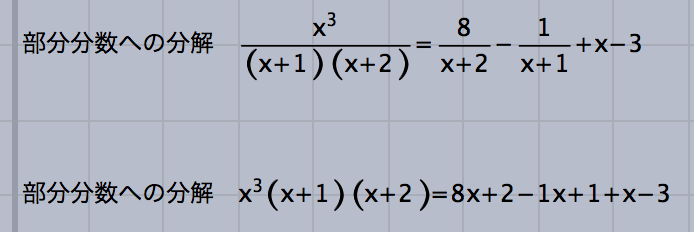
\includegraphics[bb=0 0 694 232 , width=8cm]{Fig/mxtex01.png}\\
 \\
出力したTeX挿入図では次のようになる。\\
 \\
  %%% fig.tex 2016-4-25 8:55
%%% fig.sce 2016-4-25 8:55
{\unitlength=8mm%
\begin{picture}%
(  10.22000,   3.87000)(  -0.61000,   2.03000)%
\special{pn 8}%
%
\settowidth{\Width}{部分分数への分解 $\frac{x^3}{\left(x+1\right)\,\left(x+2\right)}=\frac{8}{x+2}-\frac{1}{x+1}+x-3$}\setlength{\Width}{0\Width}%
\settoheight{\Height}{部分分数への分解 $\frac{x^3}{\left(x+1\right)\,\left(x+2\right)}=\frac{8}{x+2}-\frac{1}{x+1}+x-3$}\settodepth{\Depth}{部分分数への分解 $\frac{x^3}{\left(x+1\right)\,\left(x+2\right)}=\frac{8}{x+2}-\frac{1}{x+1}+x-3$}\setlength{\Height}{-0.5\Height}\setlength{\Depth}{0.5\Depth}\addtolength{\Height}{\Depth}%
\put(0.0500,5.0000){\hspace*{\Width}\raisebox{\Height}{部分分数への分解 $\frac{x^3}{\left(x+1\right)\,\left(x+2\right)}=\frac{8}{x+2}-\frac{1}{x+1}+x-3$}}%
%
%
\settowidth{\Width}{部分分数への分解 $\dfrac{x^3}{\left(x+1\right)\,\left(x+2\right)}=\dfrac{8}{x+2}-\dfrac{1}{x+1}+x-3$}\setlength{\Width}{0\Width}%
\settoheight{\Height}{部分分数への分解 $\dfrac{x^3}{\left(x+1\right)\,\left(x+2\right)}=\dfrac{8}{x+2}-\dfrac{1}{x+1}+x-3$}\settodepth{\Depth}{部分分数への分解 $\dfrac{x^3}{\left(x+1\right)\,\left(x+2\right)}=\dfrac{8}{x+2}-\dfrac{1}{x+1}+x-3$}\setlength{\Height}{-0.5\Height}\setlength{\Depth}{0.5\Depth}\addtolength{\Height}{\Depth}%
\put(0.0500,3.0000){\hspace*{\Width}\raisebox{\Height}{部分分数への分解 $\dfrac{x^3}{\left(x+1\right)\,\left(x+2\right)}=\dfrac{8}{x+2}-\dfrac{1}{x+1}+x-3$}}%
%
%
\end{picture}}%\\
 \\
なお,文字列を置換するのに,\verb|Assign(form,["frac","dfrac"])| ではなく,\\
Cindyscriptの文字列の関数 replace を用いて,\\
   \verb|dform=replace(form,"frac","dfrac");| \\
としてもよい。\\
 \\
例:2次関数のグラフを表示し,$x$軸との交点の$x$座標を表示する。
\begin{verbatim}
  fx="x^2-x-3";
  cmdL=[
    "ans:solve",[fx,"x"],
    "ans",[]
  ];
  CalcbyM("ans",cmdL);
  p1=indexof(ans,"[");
  p2=indexof(ans,",");
  p3=indexof(ans,"]");
  s1=substring(ans,p1,p2-1);
  s2=substring(ans,p2,p3-1);
  s1=replace(s1,"x =","");
  s2=replace(s2,"x =","");
  Mxtex("1",s1);
  Mxtex("2",s2);
  Plotdata("1",fx,"x");
  Expr([-2,-0.5],"e",tx1);
  Expr([2,-0.5],"e",tx2);
\end{verbatim}
 \\
       %%% fig.tex 2016-4-25 11:28
%%% fig.sce 2016-4-25 11:28
{\unitlength=8mm%
\begin{picture}%
(   7.07000,   5.60000)(  -3.07000,  -3.60000)%
\special{pn 8}%
%
\special{pa -564 -630}\special{pa -522 -440}\special{pa -477 -255}\special{pa -433 -82}%
\special{pa -388 79}\special{pa -343 227}\special{pa -299 362}\special{pa -254 485}%
\special{pa -210 595}\special{pa -165 693}\special{pa -121 778}\special{pa -76 850}%
\special{pa -32 910}\special{pa 13 957}\special{pa 57 992}\special{pa 102 1014}\special{pa 146 1023}%
\special{pa 191 1020}\special{pa 236 1004}\special{pa 280 976}\special{pa 325 935}%
\special{pa 369 881}\special{pa 414 815}\special{pa 458 736}\special{pa 503 645}\special{pa 547 541}%
\special{pa 592 425}\special{pa 636 296}\special{pa 681 154}\special{pa 725 0}\special{pa 770 -167}%
\special{pa 814 -347}\special{pa 859 -539}\special{pa 879 -630}%
\special{fp}%
\settowidth{\Width}{$\frac{1-\sqrt{13}}{2}$}\setlength{\Width}{0\Width}%
\settoheight{\Height}{$\frac{1-\sqrt{13}}{2}$}\settodepth{\Depth}{$\frac{1-\sqrt{13}}{2}$}\setlength{\Height}{-0.5\Height}\setlength{\Depth}{0.5\Depth}\addtolength{\Height}{\Depth}%
\put(-1.9500,-0.5000){\hspace*{\Width}\raisebox{\Height}{$\frac{1-\sqrt{13}}{2}$}}%
%
%
\settowidth{\Width}{$\frac{\sqrt{13}+1}{2}$}\setlength{\Width}{0\Width}%
\settoheight{\Height}{$\frac{\sqrt{13}+1}{2}$}\settodepth{\Depth}{$\frac{\sqrt{13}+1}{2}$}\setlength{\Height}{-0.5\Height}\setlength{\Depth}{0.5\Depth}\addtolength{\Height}{\Depth}%
\put(2.0500,-0.5000){\hspace*{\Width}\raisebox{\Height}{$\frac{\sqrt{13}+1}{2}$}}%
%
%
\special{pn 8}%
\special{pa -967 0}\special{pa 1228 0}%
\special{fp}%
\special{pn 8}%
\special{pa 1185 24}\special{pa 1260 0}\special{pa 1185 -24}\special{pa 1185 0}\special{pa 1185 24}%
\special{sh 1}\special{ip}%
\special{pn 1}%
\special{pa 1185 24}\special{pa 1260 0}\special{pa 1185 -24}\special{pa 1185 0}\special{pa 1185 24}%
\special{pa 1260 0}%
\special{fp}%
\special{pn 8}%
\special{pn 8}%
\special{pa 0 1134}\special{pa 0 -598}%
\special{fp}%
\special{pn 8}%
\special{pa 24 -555}\special{pa 0 -630}\special{pa -24 -555}\special{pa 0 -555}\special{pa 24 -555}%
\special{sh 1}\special{ip}%
\special{pn 1}%
\special{pa 24 -555}\special{pa 0 -630}\special{pa -24 -555}\special{pa 0 -555}\special{pa 24 -555}%
\special{pa 0 -630}%
\special{fp}%
\special{pn 8}%
\settowidth{\Width}{$x$}\setlength{\Width}{0\Width}%
\settoheight{\Height}{$x$}\settodepth{\Depth}{$x$}\setlength{\Height}{-0.5\Height}\setlength{\Depth}{0.5\Depth}\addtolength{\Height}{\Depth}%
\put(4.0500,0.0000){\hspace*{\Width}\raisebox{\Height}{$x$}}%
%
%
\settowidth{\Width}{$y$}\setlength{\Width}{-0.5\Width}%
\settoheight{\Height}{$y$}\settodepth{\Depth}{$y$}\setlength{\Height}{\Depth}%
\put(0.0000,2.0500){\hspace*{\Width}\raisebox{\Height}{$y$}}%
%
%
\settowidth{\Width}{O}\setlength{\Width}{-1\Width}%
\settoheight{\Height}{O}\settodepth{\Depth}{O}\setlength{\Height}{-\Height}%
\put(-0.0500,-0.0500){\hspace*{\Width}\raisebox{\Height}{O}}%
%
%
\end{picture}}%\\
 \\
 ここで,\verb|CalcbyM("ans",cmdL);| で得られるansは,次のような文字列である。\\
    \verb|"[x = -(sqrt(13)-1)/2,x = (sqrt(13)+1)/2] "|\\
そこで,ここから2つの式だけを抽出する作業を行ったのち,Mxtex() でTeXの式を得ている。\\
 さらに応用として,点AをCinderellaの作図ツールで作図し,
\begin{verbatim}
  if(A.y<0,
    fx="(x-"+text(A.x)+")^2"+guess(A.y),
    fx="(x-"+text(A.x)+")^2+"+guess(A.y);
  );
\end{verbatim}
とすると,点Aを頂点とする放物線と軸との交点の座標が描かれる。Maximaとのデータのやり取りをするためのタイムラグがあるが,インタラクティブに放物線の位置を変えることができる。\\
 \\
<参考>\\
 2次関数のような簡単な関数であれば,Cindyscriptの roots() 関数を用いて2次方程式が解けるので,次のスクリプトでほぼ同じ動作をするものを作ることができる。「ほぼ」というのは点Aの位置によっては,guess()で解釈しきれないことがあるためである。Maximaを使えば数式処理で解を求めるので,Aがどこにあってもきれいに表示できる。
\begin{verbatim}
  fx="x^2-2*A.x*x+A.x^2+A.y";
  cf=[A.x^2+A.y,-2*A.x,1];
  sol=roots(cf);
  s1=guess(sol_2);
  s2=guess(sol_1);
  Mxtex("1",s1);
  Mxtex("2",s2);
  Plotdata("1",fx,"x");
  Expr([-2,-0.5],"e",tx1);
  Expr([2,-0.5],"e",tx2);
\end{verbatim}

\end{description}

\begin{flushright} \hyperlink{functionlist}{$\Rightarrow$関数一覧}\end{flushright}
\newpage


% Scilabとの連携 ==================================
\subsection{Scilabとの連携}
 KeTCindyは,もともと Scilab と連携して,Cinderellaからの出力をTeXのテキストとするシステムである。しかし,それだけでなく,Maximaなどとの連携と同様,Scilab の関数を実行して,データをやりとりすることができる。\\
 KeTCindyでは,kc.bat/shによってコマンドをScilabに渡し,結果をテキストファイルで受け取る。このとき,Scilabとのやりとりで,次のようなファイルが作業ディレクトリに作成される。\\
拡張子 sci :Scilab用のファイル\\
拡張子 txt:データファイル\\
このデータのやり取りに関する次のオプションがある。\\
 オプションなしまたは,”” のとき\\
  i) データファイルがなければ,新しく作る\\
  ii) データファイルが既にあればそれを読み込む\\
 "m"  のとき,強制的にデータファイルを作り直す。\\
 "r" のとき,すでにあるデータファイルを読み込む。\\ 
 このとき,ファイルの読み書きで不具合があると,数秒の後「==$>$ file.txt not generated (5 s ) 」のようなエラーメッセージがコンソールに表示される。このような場合は作業ディレクトリの設定などを確認していただきたい。この待ち時間については,Waitオプションで設定することもできる。\\

\begin{description}

\hypertarget{calcbyS}{}
\item[関数] CalcbyS(name,コマンド,option)
\item[機能] Scilabのコマンドスクリプトを実行する
\item[説明] 第2引数はScilabで実行するコマンドのリスト。\\
 \\
\hypertarget{plotdataS}{}
\item[関数] PlotdataS(name,関数,変数)
\item[機能] Plotdataと同様の書式で,Scilabの関数を実行する
\item[説明] Cindyscriptの組込関数にない関数のグラフを描くことができる。\\
 \\
例:ベッセル関数のグラフを描く
\begin{verbatim}
  PlotdataS("1","besselj(1,x)","x");
\end{verbatim}

\end{description}
\begin{flushright} \hyperlink{functionlist}{$\Rightarrow$関数一覧}\end{flushright}
\newpage
% Risa/Asirとの連携 ==================================
\subsection{Risa/Asirとの連携}

\begin{description}

\hypertarget{calcbyA}{}
\item[関数] CalcbyA(name,コマンド,option)
\item[機能] Risa/Asirのスクリプトを実行する
\item[説明] 第2引数はRisa/Asirで実行するコマンド。\\
 コマンドと引数リストの繰り返しからなるリスト(例えばcmdL)を作って,一度に実行する。\\
 戻り値はない。(未定義値) 結果は,コマンドリストの最後に記述した変数(引数は空リスト)の値がname で指定された変数に代入される。複数の結果を戻すときは,:: で区切って記述するとリストにして代入される。\\

\hypertarget{asirfun}{}
\item[関数] Asirfun(name,式,リスト,option)
\item[機能] Risa/Asirの関数を実行する
\item[説明] 第2引数の「式」はRisa/Asirの関数名。第3引数のリストは関数に渡す引数のリスト。\\
 戻り値は,第1引数の式に1つでも文字があると文字列となる。すべて数字(+,-, . を含む)の場合は
16桁以下であれば数,それ以上の場合は文字列となる。また,戻り値は,変数 asname にも代入される。\\
オプションに "Disp=no" をつけると,結果をコンソールに表示しない。\\

\end{description}
\begin{flushright} \hyperlink{functionlist}{$\Rightarrow$関数一覧}\end{flushright}
\newpage
% FriCASとの連携 ==================================
\subsection{FriCAS(Axiom)との連携}

\begin{description}

\hypertarget{calcbyF}{}
\item[関数] CalcbyF(name,コマンド,option)
\item[機能] FriCASのスクリプトを実行する
\item[説明] 第2引数はFriCASで実行するコマンド。\\
 コマンドと引数リストの繰り返しからなるリスト(例えばcmdL)を作って,一度に実行する。\\
 戻り値はない。(未定義値) 結果は,コマンドリストの最後に記述した変数(引数は空リスト)の値がname で指定された変数に代入される。複数の結果を戻すときは,:: で区切って記述するとリストにして代入される。\\

\hypertarget{frfun}{}
\item[関数] Frfun(name,式,リスト,option)
\item[機能] FriCASの関数を実行する
\item[説明] 第2引数の「式」はFriCASの関数名。第3引数のリストは関数に渡す引数のリスト。\\
 戻り値は,第1引数の式に1つでも文字があると文字列となる。すべて数字(+,-, . を含む)の場合は
16桁以下であれば数,それ以上の場合は文字列となる。また,戻り値は,変数 friname にも代入される。\\
オプションに "Disp=no" をつけると,結果をコンソールに表示しない。\\

\end{description}
\begin{flushright} \hyperlink{functionlist}{$\Rightarrow$関数一覧}\end{flushright}

\newpage
% 表計算ソフトとの連携 ==================================
\subsection{表計算ソフトとの連携}
 表計算ソフトでは,複数のセルを選択してコピー(Windowsでは Crtl+ C ,Macでは Command+C)すると,セルの内容はtab区切りのテキストデータとしてクリップボードにコピーされる。これをCindyscriptエディタにペーストすることで表計算ソフトのデータをKeTCindyで利用できる。逆に,Cindyscriptのコンソールへの出力を表計算ソフトのシートにコピーすることもできる。

\begin{description}
\hypertarget{tab2list}{}
\item[関数] Tab2list(str,option)
\item[機能] str の内容をリストに変換する
\item[説明] tab区切りになっている文字列 str をリストに変換する。\\
 optionは,NULLのセルの置き換え。リストで表す。デフォルトは[0]。\\
次のような手順で表計算ソフトからデータをKeTCindyに写すことができる。\\
 \\
(1) 表計算ソフトで,適当な範囲を指定しクリップボードにコピーする。\\
 Windowsなら Ctrl+C,Macなら Command+C\\
 \\
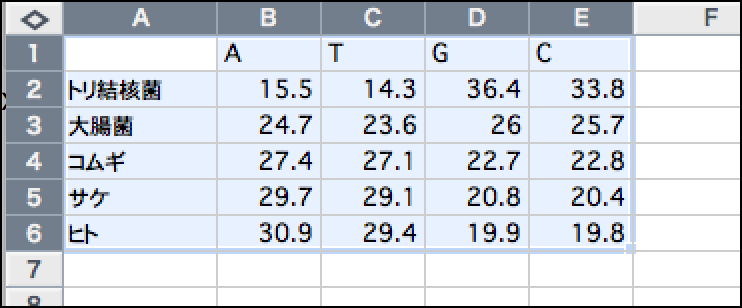
\includegraphics[bb=0 0 742 308 , width=8cm]{Fig/tab2list01.png}\\
 \\
(2) Cindyscriptエディタで,適当な文字変数を用意する。\\
 たとえば,data="";\\
 \\
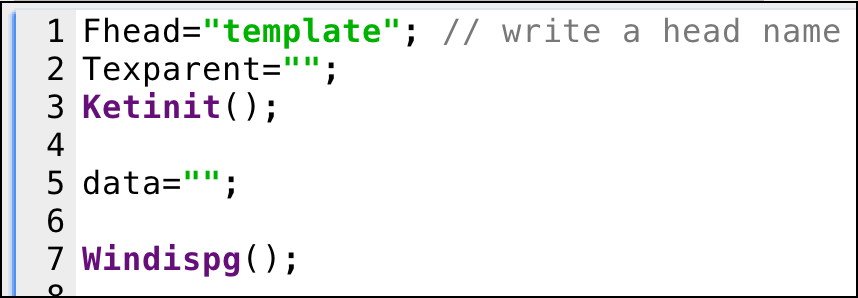
\includegraphics[bb=0 0 858 298 , width=10cm]{Fig/tab2list02.png}\\
 \\
(3) ここにペーストすると,文字列にコピーされる。\\
 もし,右のようになったら(表計算ソフトによります)左のように,最後の "" の前で改行しておく。\\
 \\
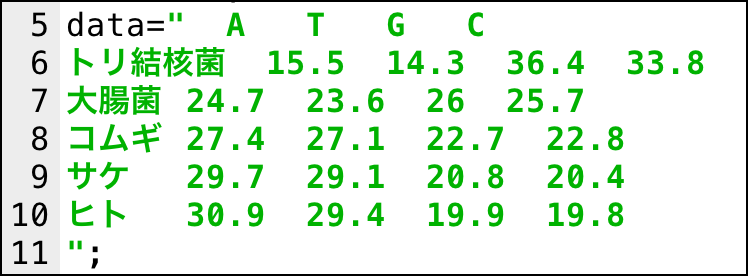
\includegraphics[bb=0 0 748 276 , width=6cm]{Fig/tab2list001.png} 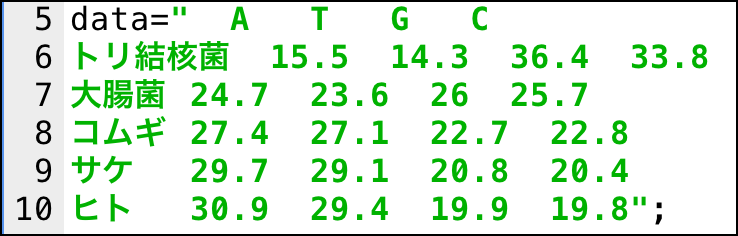
\includegraphics[bb=0 0 738 236 , width=6cm]{Fig/tab2list00.png}\\

 \\
(4) この文字変数 data に対し,Tab2list(data) を実行すると,行列を表すリストが返される。\\
 これを適当な変数に代入し,作表コマンドで表にするなど,目的に応じて利用する。\\
 数値だけなら行列として計算もできる。\\
 \\
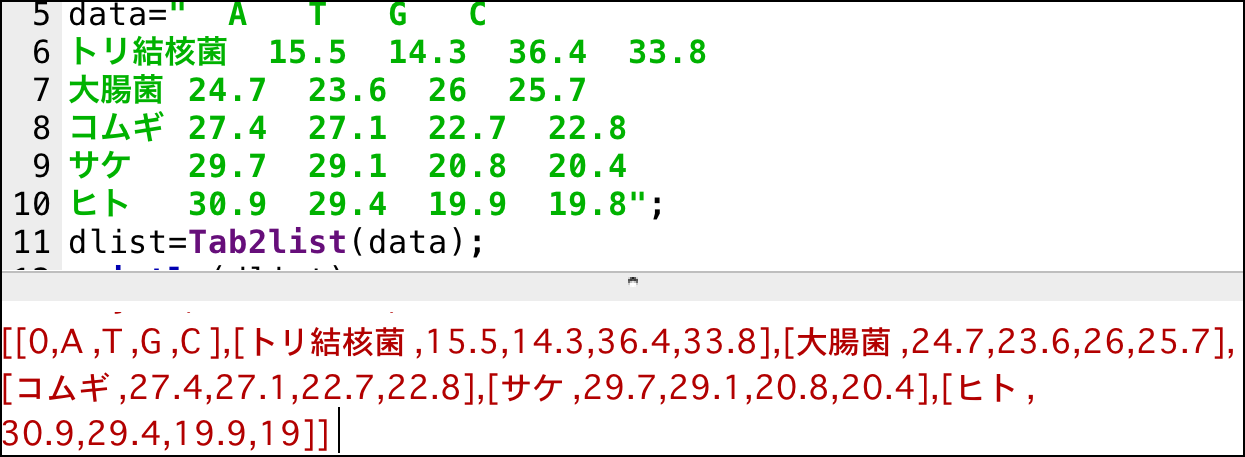
\includegraphics[bb=0 0 1245 457 , width=10cm]{Fig/tab2list03.png}

\hypertarget{dispmat}{}
\item[関数] Dispmat(list)
\item[機能] リストを行列の形でtab区切りにしてコンソールに表示する。
\item[説明] 行列を表すリスト (たとえば dlist) を引数としてDispmat(dlist) を実行すると,コンソールに行列型で内容が表示される。\\
 実際にはTAB区切りの文字列。(println としなくても直接コンソールに表示される)\\
 これを表計算ソフトのシートにコピーする。\\
 \\
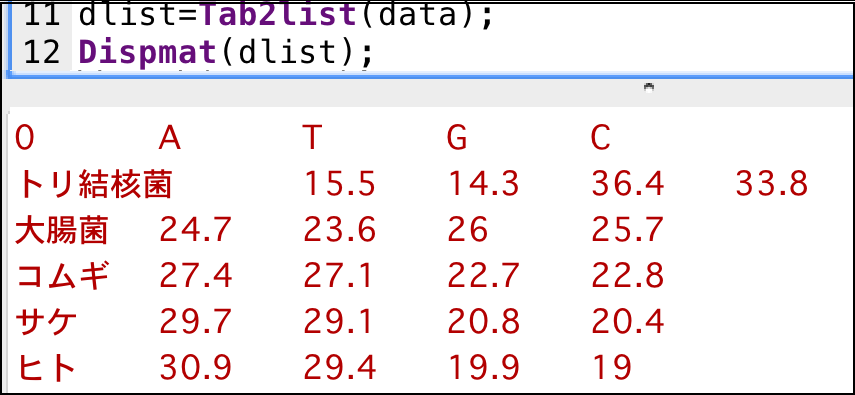
\includegraphics[bb=0 0 855 395 , width=8cm]{Fig/tab2list04.png}\

\end{description}
\newpage
% MeshLabとの連携 ==================================
%\subsection{MeshLabとの連携}

% アニメーション ==================================
\section{アニメーションPDF:KeTCindymv}
\subsection{概要}
アニメーションのできるPDFを作る。

Cinderellaの作図機能とCindyscriptを用いてアニメーションができるが,PDFにすることでCinderellaがなくてもPDFビュアーがあればアニメーションを実行できるので,プレゼンテーションや教材の受け渡しなどに便利である。

KeTCindymvの画面は次のようになっている。(templatemv.cdy)\\
 \\
  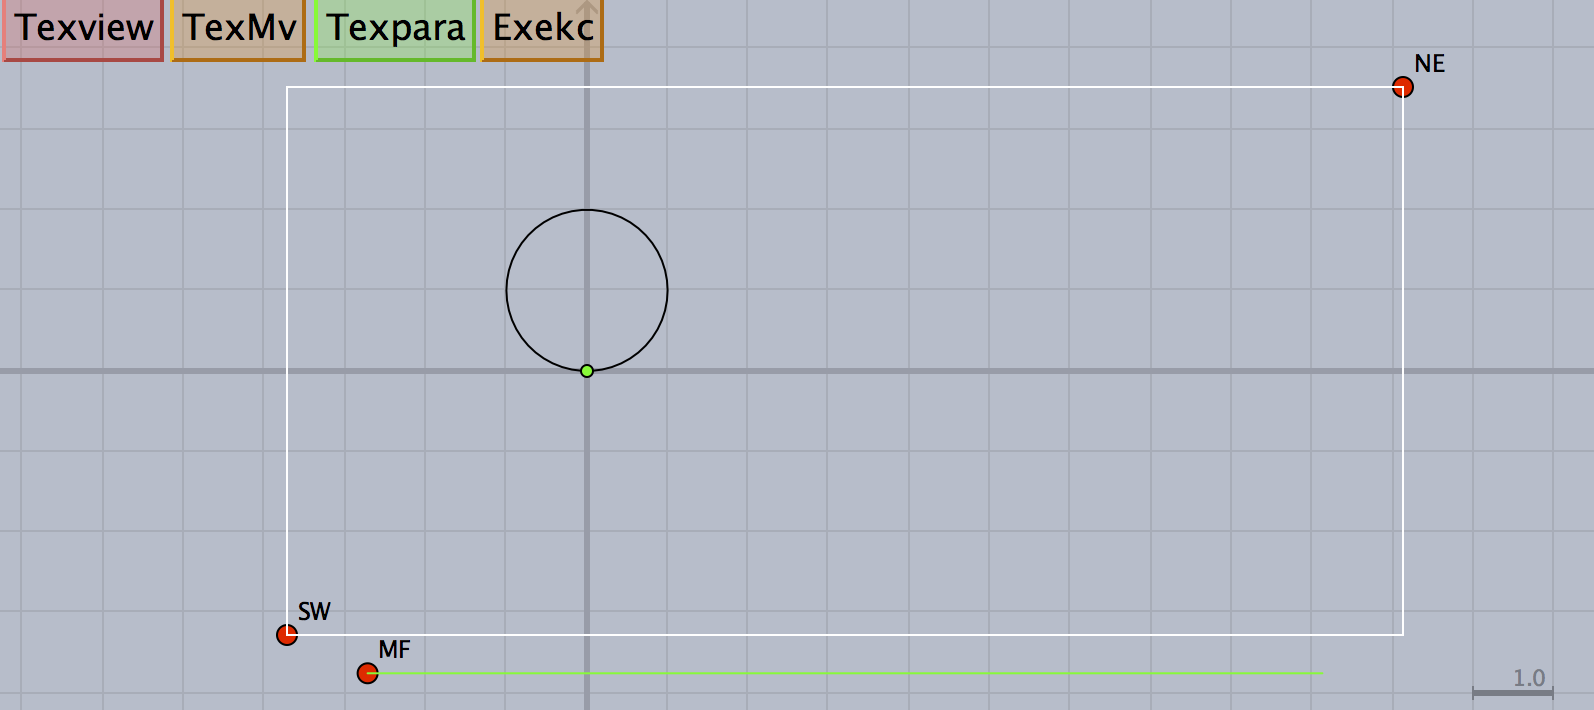
\includegraphics[bb=0 0 1594 710 , width=12cm]{Figmv/mvgaiyou01.png}

画面上方のボタンには,次のようなスクリプトが割り当てられているので,ボタンを自作することもできる。

\begin{tabbing}
 12345678978\=1234567897890123\=\kill
 Texview  \>: Viewtex(); \>現在の画面のPDFデータを作る\\
 TexMv  \>: Texmovie(); \>アニメーションPDFデータを作る\\
 Texpara \>: Texpara(); \>フレームに分割したPDFデータを作る\\
 Exekc  \>: kc(); \>バッチファイルを実行する
\end{tabbing}

アニメーションの作成は,フレームを定義する関数を作成し,Moviedata() 関数を実行する。実行後,TexMv,Exekc のボタンを順に押すことで,Fhead+"moviefigs.tex" と Fhead+"moviemain.tex",Fhead+"moviemain.pdf" が生成されて表示される。たとえば,Fhead が "abc" の場合,TeX の文書には\\
     \verb|\input{abcmoviefigs.tex}|\\
で動画を挿入することができる。

ただし,動画のできるPDFを作成するには,ドキュメントクラスと使用パッケージについて注意が必要である。

ドキュメントクラスは,article または jarticle とする。jsarticle は使えない。

パッケージは animate に dvipdfmx オプションをつける。\\
      \verb|\usepackage[dvipdfmx]{animate}|

また,アニメーションPDFでアニメーションを行うにはAdobe Acrobat Reader など,アニメーションに対応したPDFリーダーが必要である。WindowsのSumatraPDF,Macの プレビューでは動かない。\\

次に,Texpara,Exekc のボタンを順に押すことで,フレームに分割した Fhead+"parafigs.tex" と Fhead+"paramain.tex" ,Fhead+"paramain.pdf" が生成されて表示される。この図を利用するにはパッケージの指定がやや面倒である。 Fhead+"mvparamain.tex" を参照されたい。 \\

画面下方のスライダによりアニメーションの途中図を描くことができる。Texview と Exekc ボタンによりその図のファイルが作成される。


\subsection{設定}
KeTCindymvでは,KeTCindyと若干異なる設定が必要である。

まず,Initialization スロットでは,KeTCindy で\\
  \verb|Shellfile="";|\\
になっているのを\\
  \verb| Shellfile="mv";|\\
とする。

次に,Draw スロットでは,次のように \verb|Ketinit();| に加え,\verb|Ketinitmv();| が必要である。また,画面表示のために,\verb|Windispg();| のかわりに \verb|Mvdispg();| を用いる。
\begin{verbatim}
 Fhead="templatemv";
 Texparent="";
 Ketinit();
 Ketinitmv();

  ここにスクリプトを書く

 Mvdispg();
\end{verbatim}
なお,ひながたの templatemv.cdy ではこの設定がすでにしてある。

\newpage
\subsection{描画}
\begin{description}

\hypertarget{moviedata}{}
\item[関数] Moviedata(str1,str2,options)
\item[機能] アニメーションデータを作る
\item[説明] str1 はアニメーションを定義する関数名を文字列とする。str2 は定義域。\\
 optionsは,Cut と Div \\
 Cut : 1秒のフレーム数。初期値は20。\\
 Civ : 全体のフレーム数。初期値は80。\\
 したがって,初期値では4秒間のアニメーションとなる。\\
 \\
【例】定円上を動く点Pと,定点Aを結ぶ線分の中点をQとして動きを見る。\\
まず,定円を,原点中心、半径2として描いておく。\\
アニメーションを定義する関数は,時間を $t$ とすれば,時刻 $t$ における図(動くものだけ)を定義する。時刻は単なる媒介変数であるので,$t$ でなく $s$ などでもよい。
\begin{verbatim}
 Mf(t):=(
   pt=2*[cos(t),sin(t)];
   Listplot("2",[[4,0],pt]);
   Pointdata("2",mid(pt,[4,0]));
   Letter([[4,0],"s","A",pt,"en","P",mid(pt,[4,0]),"ne","Q"]);
 );
\end{verbatim}
ここで,\verb|Mf(t)| の中で使っているユーザー定義関数\verb|mid()| は,端点を引数として線分の中点を返すもので,\\
  \verb|mid(p1,p2):=(p1+p2)/2;|\\
として定義しておく。\\
また,点の大きさを適宜設定しておく。\\
以上の準備の後,\\
  \verb|Moviedata("Mf(t)","t=[0,2*pi]");|\\
を実行する。\\
ここでは,角度を媒介変数としているので,時間の$t$ でなく$s$ として\\
  \verb|Moviedata("Mf(s)","s=[0,2*pi]");|\\
としてもよい。\\
次のようにオプションを指定すると,5秒間のアニメーションとなる。\\
  \verb|Moviedata("Mf(s)","s=[0,2*pi]",["Div=50","Cut=10"]);|\\
\verb|["Div=150","Cut=30"]|とすると,やはり5秒間のアニメーションとなるが,1秒間のフレーム数が多いためなめらかな動きとなる。ビデオのフレームレートである。ただし,ファイルサイズは約3倍となる。\\
Cinderellaの画面は次のようになる。\\
 \\
  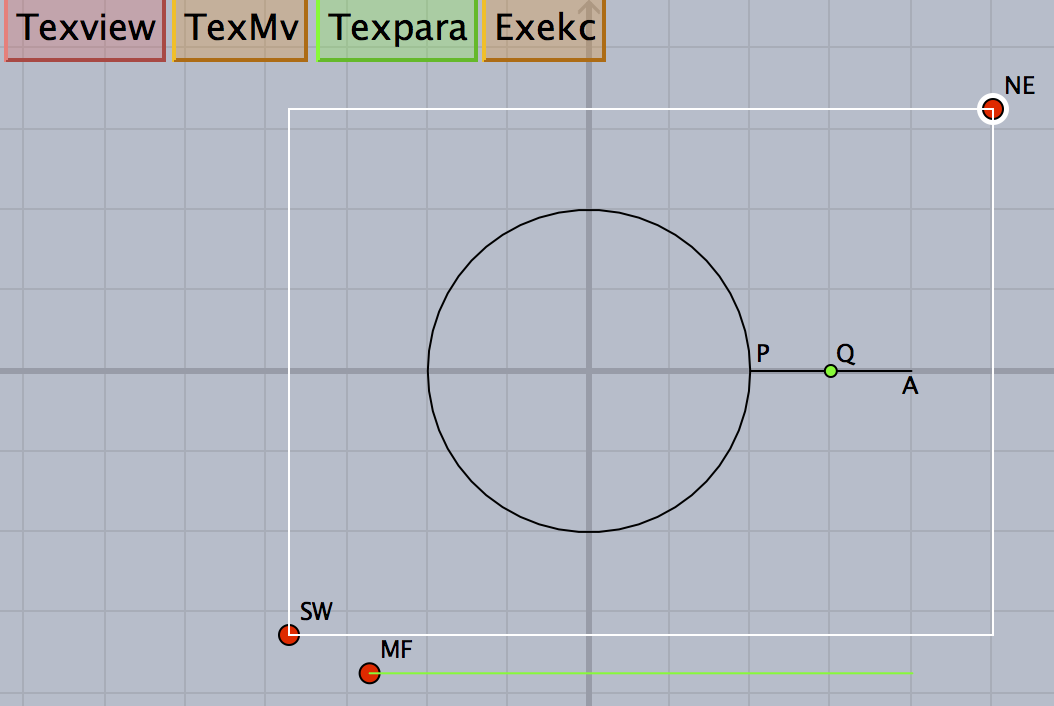
\includegraphics[bb=0 0 1054 706 , width=8cm]{Figmv/moviedata01.png}\\
 \\
TexMvボタン または TexParaボタンを押すと画面上でもアニメーションが実行される。その後 Exekc ボタンを押すとファイルが作成される。

この図では,点が明示されるのは Q だけである。A,Pとも点を明示する場合のスクリプトの全体を示しておく。
\begin{verbatim}
 Fhead="mid";
 Texparent="";
 Ketinit();
 Ketinitmv();
 mid(p1,p2):=(p1+p2)/2;
 Circledata("1",[[0,0],[2,0]]);
 Ptsize(4);
 Pointdata("1",[4,0]);
 Mf(t):=(
   pt=2*[cos(t),sin(t)];
   Listplot("2",[[4,0],pt]);
   Pointdata("2",pt);
   Pointdata("3",mid(pt,[4,0]));
   Letter([[4,0],"s","A",pt,"en","P",mid(pt,[4,0]),"ne","Q"]);  
 );
 Moviedata("Mf(s)","s=[0,2*pi]",["Div=30","Cut=10"]);
 Mvdispg();
\end{verbatim}
\begin{flushright} \hyperlink{functionlist3d}{$\Rightarrow$関数一覧}\end{flushright}

\end{description}

\newpage


%== 3D ===============
\section{\ketcindy 3D}
\subsection{概要}
\ketcindy 3Dの画面は次のように構成される。

Cinderellaの描画面に,白の矩形で囲んだ領域が2つできる。NE,SWを対角とする左側の領域を主画面,右側の領域を副画面という。\\

      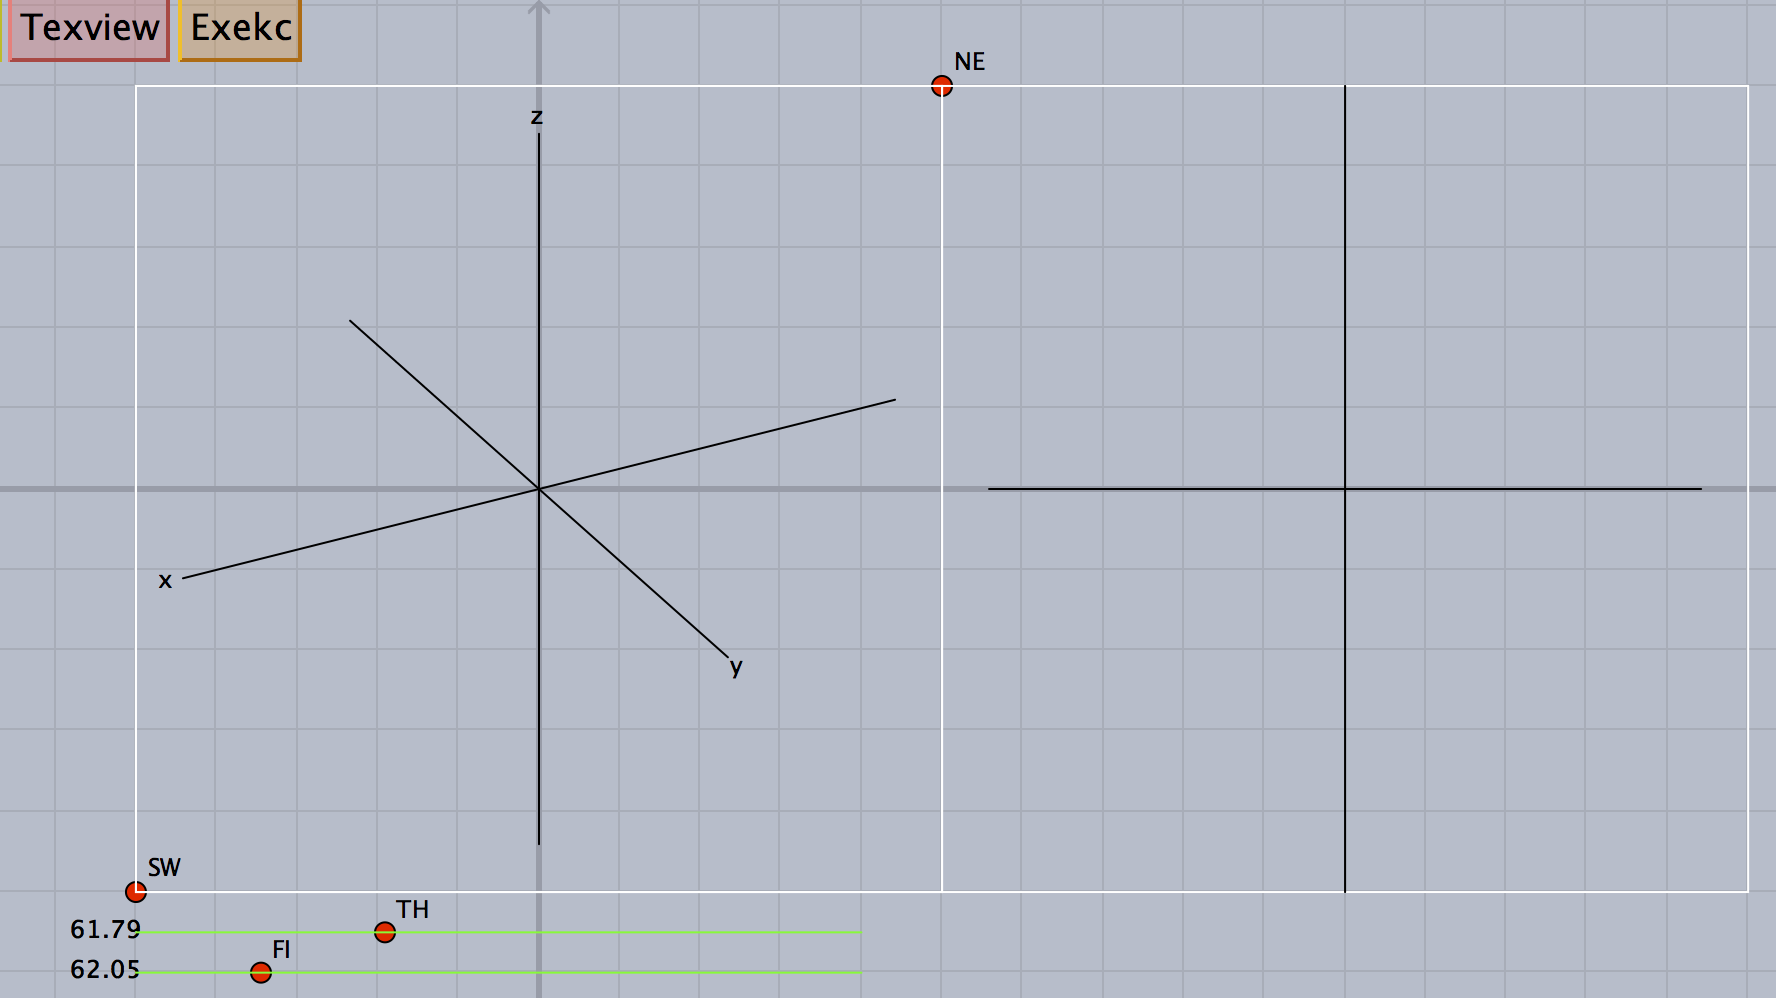
\includegraphics[bb=0 0 1776 998 , width=8cm]{Fig3d/3dstart.png}\\

主画面は平面の場合と同様,TeXに出力される範囲を示し,NE,SWの2点をドラッグすることにより変更できる。

副画面は,Start3d() 関数により作成される。座標軸は,Xyzax3data() 関数によって描くことができる。主画面の下方のスライダで視点が移動でき,主画面上では軸が回転する。副画面は,xy平面上に視点を置いたものと考えればよい。

主画面上にCinderellaの作図ツールで点や線分を作図すると,Start3d() 関数により副画面に対応する点が作図される。主画面上の点をドラッグするとx,y座標を変更でき,副画面上の点をドラッグするとz座標を変更できる。空間内の点は,Putpoint3d()関数によって座標を指定して作成することもできる。次のような図はCinderellaの作図ツールだけでも作ることができるし,Putpoint3d()関数を用いても作ることができる。\\

  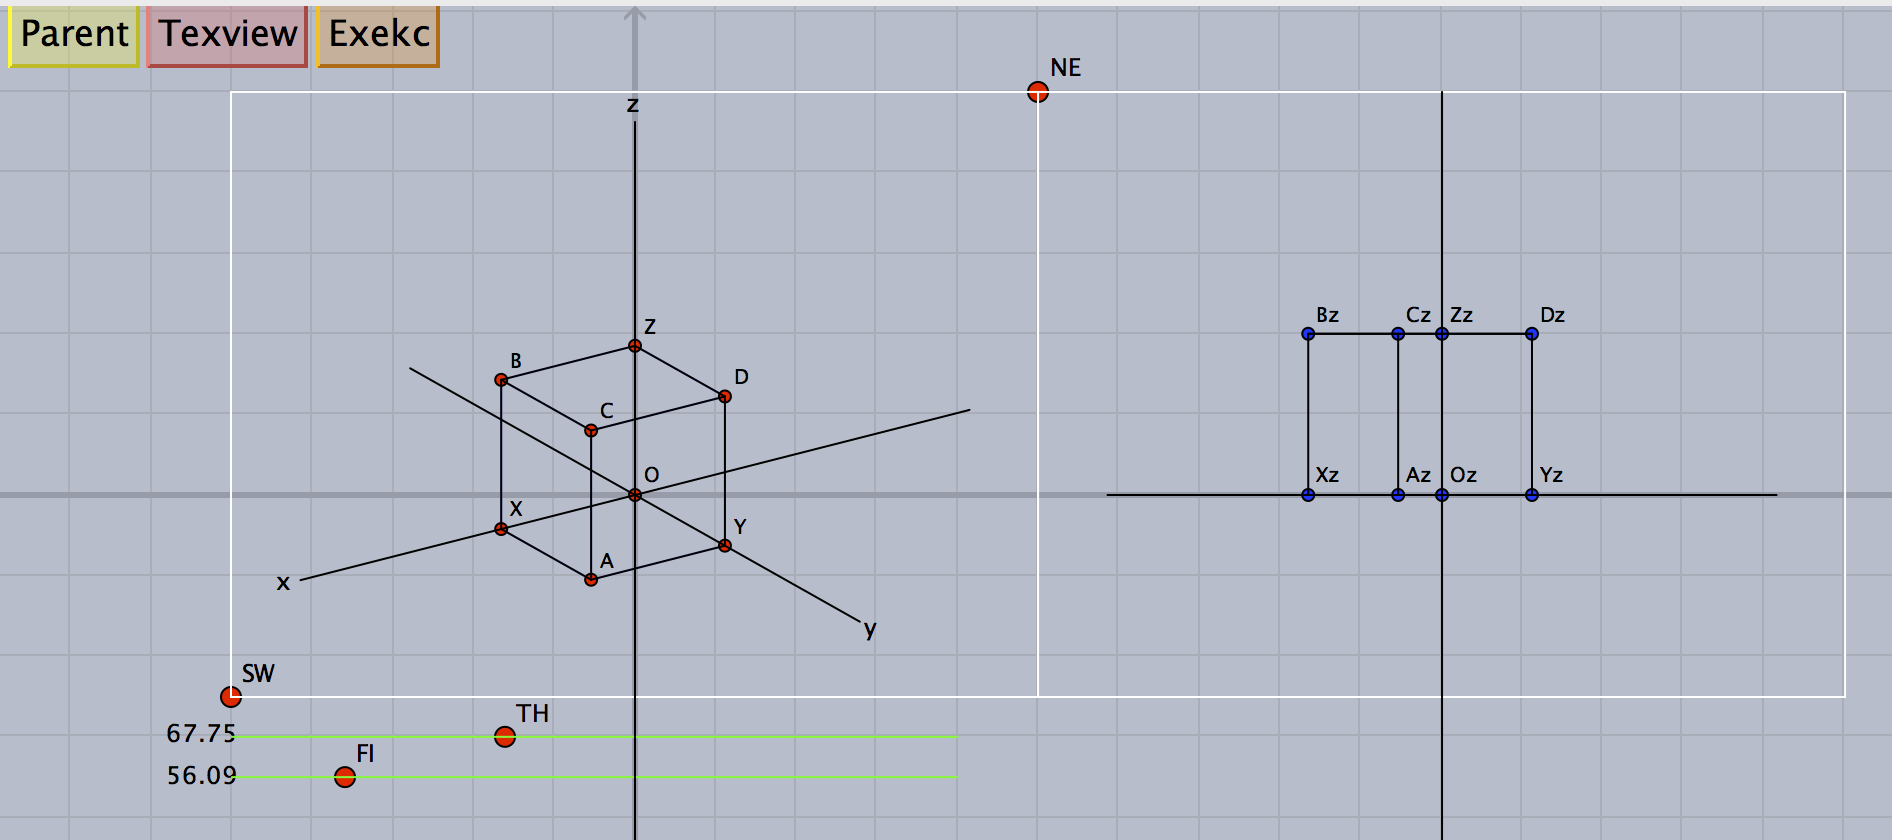
\includegraphics[bb=0 0 1892 840 , width=10cm]{Fig3d/3dscreen.png}\\

主画面と副画面の対応する点をドラッグすることにより,インタラクティブに図形を描くことができるが、実際には描画関数を用いて図形を描き,スライダで視点を変えて見やすい図をTeXに出力することになるだろう。

KeTCindy3Dでは,点・直線・曲線・面の描画を描画関数を用いて行うことができる。線や面については陰線処理を行い,立体的な図を作成することができる。しかし,陰線処理は処理にかなりの時間がかかるので,CindyscriptではなくScilabで行っているが,それでも相当時間がかかることを覚悟しなければならない。Scilabでの計算は,バッチファイル/シェルファイルで行っているが,Cindyscriptではその計算結果が出るのを待つため一時的に反応がなくなる。したがって,反応がなくなってもハングアップではないので,Cinderellaを強制終了しないように。

一例を示すと,球面をメッシュ入りで座標軸とともに陰線処理して描いた場合,次のような図が画面に表示されるまでの時間は,MacBookPro13' (Late 2013) Core i7 2.8GHz 8GB (OSX 10.11.6) の場合で約124秒であった。スクリプトは \hyperlink{wireparadata}{Wireparadata() } の例を参照されたい。\\
            %%% /Users/Hannya/ketcindy/ketwork/template.tex 2016-8-22 22:0
%%% template.sce 2016-8-22 22:0
{\unitlength=8mm%
\begin{picture}%
(   7.17000,   6.03000)(  -3.65000,  -2.44000)%
\special{pn 8}%
%
\settowidth{\Width}{$x$}\setlength{\Width}{-0.5\Width}%
\settoheight{\Height}{$x$}\settodepth{\Depth}{$x$}\setlength{\Height}{-0.5\Height}\setlength{\Depth}{0.5\Depth}\addtolength{\Height}{\Depth}%
\put(-3.2384,-1.6002){\hspace*{\Width}\raisebox{\Height}{$x$}}%
%
%
\settowidth{\Width}{$y$}\setlength{\Width}{-0.5\Width}%
\settoheight{\Height}{$y$}\settodepth{\Depth}{$y$}\setlength{\Height}{-0.5\Height}\setlength{\Depth}{0.5\Depth}\addtolength{\Height}{\Depth}%
\put(3.3633,-2.3750){\hspace*{\Width}\raisebox{\Height}{$y$}}%
%
%
\settowidth{\Width}{$z$}\setlength{\Width}{-0.5\Width}%
\settoheight{\Height}{$z$}\settodepth{\Depth}{$z$}\setlength{\Height}{-0.5\Height}\setlength{\Depth}{0.5\Depth}\addtolength{\Height}{\Depth}%
\put(0.0000,2.6107){\hspace*{\Width}\raisebox{\Height}{$z$}}%
%
%
\special{pa -363 515}\special{pa -348 525}\special{pa -302 553}\special{pa -286 561}%
\special{pa -243 581}\special{pa -207 595}\special{pa -189 601}\special{pa -137 615}%
\special{pa -87 624}\special{pa -70 626}\special{pa -39 629}\special{pa 9 630}\special{pa 57 627}%
\special{pa 70 626}\special{pa 105 621}\special{pa 156 610}\special{pa 208 594}\special{pa 264 572}%
\special{pa 286 561}\special{pa 324 540}\special{pa 348 525}\special{pa 386 498}\special{pa 400 487}%
\special{pa 444 447}\special{pa 451 439}\special{pa 482 405}\special{pa 515 362}\special{pa 545 316}%
\special{pa 569 270}\special{pa 589 222}\special{pa 605 174}\special{pa 613 143}\special{pa 617 125}%
\special{pa 625 75}\special{pa 629 25}\special{pa 630 9}\special{pa 629 -25}\special{pa 625 -75}%
\special{pa 617 -125}\special{pa 605 -174}\special{pa 589 -222}\special{pa 579 -248}%
\special{pa 569 -270}\special{pa 545 -316}\special{pa 524 -350}\special{pa 516 -361}%
\special{pa 483 -405}\special{pa 460 -430}\special{pa 444 -447}\special{pa 400 -487}%
\special{pa 348 -525}\special{pa 332 -535}\special{pa 286 -561}\special{pa 272 -568}%
\special{pa 216 -592}\special{pa 208 -595}\special{pa 163 -609}\special{pa 112 -620}%
\special{pa 71 -626}\special{pa 63 -627}\special{pa 15 -630}\special{pa -33 -629}%
\special{pa -71 -626}\special{pa -81 -625}\special{pa -130 -616}\special{pa -182 -603}%
\special{pa -207 -595}\special{pa -236 -584}\special{pa -287 -561}\special{pa -294 -557}%
\special{pa -348 -525}\special{pa -355 -521}\special{pa -399 -487}\special{pa -419 -471}%
\special{pa -444 -447}\special{pa -483 -405}\special{pa -516 -361}\special{pa -545 -316}%
\special{pa -569 -270}\special{pa -589 -222}\special{pa -595 -206}\special{pa -605 -174}%
\special{pa -617 -125}\special{pa -625 -77}\special{pa -629 -25}\special{pa -629 25}%
\special{pa -627 59}\special{pa -625 75}\special{pa -617 125}\special{pa -605 174}%
\special{pa -601 189}\special{pa -589 222}\special{pa -569 270}\special{pa -553 302}%
\special{pa -545 316}\special{pa -516 361}\special{pa -492 393}\special{pa -483 405}%
\special{pa -444 447}\special{pa -427 463}\special{pa -399 487}\special{pa -363 515}%
\special{fp}%
\special{pa 0 -508}\special{pa -30 -492}\special{pa -61 -474}\special{pa -91 -455}%
\special{pa -120 -433}\special{pa -149 -410}\special{pa -178 -385}\special{pa -206 -358}%
\special{pa -233 -330}\special{pa -259 -301}\special{pa -284 -271}\special{pa -308 -239}%
\special{pa -331 -207}\special{pa -352 -174}\special{pa -372 -140}\special{pa -391 -106}%
\special{pa -408 -71}\special{pa -423 -36}\special{pa -437 0}\special{pa -449 35}%
\special{pa -460 70}\special{pa -468 105}\special{pa -475 139}\special{pa -479 173}%
\special{pa -482 206}\special{pa -483 239}\special{pa -482 270}\special{pa -479 301}%
\special{pa -475 330}\special{pa -468 358}\special{pa -460 384}\special{pa -449 409}%
\special{pa -437 432}\special{pa -423 454}\special{pa -408 474}\special{pa -391 492}%
\special{pa -372 508}\special{pa -352 522}\special{pa -331 534}\special{pa -308 544}%
\special{fp}%
\special{pa -116 -436}\special{pa -103 -428}\special{pa -88 -421}\special{pa -72 -415}%
\special{pa -55 -411}\special{pa -37 -407}\special{pa -18 -405}\special{pa 1 -404}%
\special{pa 20 -405}\special{pa 38 -407}\special{pa 56 -411}\special{pa 73 -416}\special{pa 89 -422}%
\special{pa 104 -429}\special{pa 117 -437}\special{pa 128 -446}\special{pa 137 -456}%
\special{pa 144 -466}\special{pa 148 -477}\special{pa 150 -488}\special{pa 150 -500}%
\special{pa 148 -511}\special{pa 143 -521}\special{pa 136 -532}\special{pa 127 -542}%
\special{pa 116 -551}\special{pa 103 -559}\special{pa 88 -566}\special{pa 72 -572}%
\special{pa 55 -576}\special{pa 37 -580}\special{pa 18 -582}\special{pa -1 -583}\special{pa -20 -582}%
\special{pa -38 -580}\special{pa -56 -576}\special{pa -73 -571}\special{pa -89 -565}%
\special{pa -104 -558}\special{pa -117 -550}\special{pa -128 -541}\special{pa -137 -531}%
\special{pa -144 -521}\special{pa -148 -510}\special{pa -150 -499}\special{pa -150 -487}%
\special{pa -148 -476}\special{pa -143 -466}\special{pa -136 -455}\special{pa -127 -445}%
\special{pa -116 -436}%
\special{fp}%
\special{pa -225 -339}\special{pa -199 -323}\special{pa -171 -310}\special{pa -140 -298}%
\special{pa -106 -289}\special{pa -71 -282}\special{pa -35 -278}\special{pa 2 -277}%
\special{pa 38 -279}\special{pa 74 -283}\special{pa 109 -290}\special{pa 142 -299}%
\special{pa 173 -311}\special{pa 202 -325}\special{pa 227 -341}\special{pa 248 -358}%
\special{pa 266 -377}\special{pa 279 -398}\special{pa 288 -419}\special{pa 292 -440}%
\special{pa 292 -462}\special{pa 287 -483}\special{pa 278 -504}\special{pa 264 -525}%
\special{pa 246 -544}\special{pa 225 -561}\special{pa 199 -577}\special{pa 171 -591}%
\special{pa 140 -602}\special{pa 106 -611}\special{pa 71 -618}\special{pa 35 -622}%
\special{pa -2 -623}\special{pa -38 -621}\special{pa -74 -617}\special{pa -109 -610}%
\special{pa -142 -601}\special{pa -173 -589}\special{pa -202 -575}\special{pa -227 -560}%
\special{pa -248 -542}\special{pa -266 -523}\special{pa -279 -503}\special{pa -288 -482}%
\special{pa -292 -460}\special{pa -292 -438}\special{pa -287 -417}\special{pa -278 -396}%
\special{pa -264 -376}\special{pa -246 -357}\special{pa -225 -339}%
\special{fp}%
\special{pa -320 -222}\special{pa -284 -200}\special{pa -244 -180}\special{pa -199 -164}%
\special{pa -152 -151}\special{pa -102 -141}\special{pa -50 -135}\special{pa 2 -134}%
\special{pa 55 -136}\special{pa 106 -142}\special{pa 156 -152}\special{pa 203 -165}%
\special{pa 247 -182}\special{pa 288 -202}\special{pa 323 -224}\special{pa 354 -249}%
\special{pa 379 -277}\special{pa 398 -305}\special{pa 411 -336}\special{pa 417 -366}%
\special{pa 417 -397}\special{pa 410 -428}\special{pa 397 -458}\special{pa 377 -487}%
\special{pa 351 -514}\special{pa 320 -539}\special{pa 284 -561}\special{pa 244 -581}%
\special{pa 199 -597}\special{pa 152 -610}\special{pa 102 -620}\special{pa 50 -625}%
\special{pa -2 -627}\special{pa -55 -625}\special{pa -106 -619}\special{pa -156 -609}%
\special{pa -203 -596}\special{pa -247 -579}\special{pa -288 -559}\special{pa -323 -537}%
\special{pa -354 -512}\special{pa -379 -484}\special{pa -398 -455}\special{pa -411 -425}%
\special{pa -417 -395}\special{pa -417 -364}\special{pa -410 -333}\special{pa -397 -303}%
\special{pa -377 -274}\special{pa -351 -247}\special{pa -320 -222}%
\special{fp}%
\special{pa -398 -92}\special{pa -353 -64}\special{pa -302 -40}\special{pa -247 -20}%
\special{pa -188 -3}\special{pa -126 8}\special{pa -62 15}\special{pa 3 17}\special{pa 68 15}%
\special{pa 132 7}\special{pa 193 -5}\special{pa 252 -21}\special{pa 307 -42}\special{pa 357 -67}%
\special{pa 401 -95}\special{pa 439 -126}\special{pa 470 -160}\special{pa 494 -196}%
\special{pa 510 -233}\special{pa 518 -271}\special{pa 517 -310}\special{pa 509 -348}%
\special{pa 492 -385}\special{pa 468 -421}\special{pa 436 -454}\special{pa 398 -485}%
\special{pa 353 -513}\special{pa 327 -526}%
\special{fp}%
\special{pa -344 -517}\special{pa -357 -511}\special{pa -401 -483}\special{pa -439 -451}%
\special{pa -470 -418}\special{pa -494 -382}\special{pa -510 -344}\special{pa -518 -306}%
\special{pa -517 -268}\special{pa -509 -230}\special{pa -492 -193}\special{pa -468 -157}%
\special{pa -436 -123}\special{pa -398 -92}%
\special{fp}%
\special{pa -452 43}\special{pa -401 75}\special{pa -344 102}\special{pa -281 126}%
\special{pa -214 144}\special{pa -143 157}\special{pa -71 165}\special{pa 3 168}\special{pa 77 165}%
\special{pa 150 156}\special{pa 220 143}\special{pa 287 124}\special{pa 349 100}\special{pa 406 72}%
\special{pa 456 40}\special{pa 499 5}\special{pa 534 -34}\special{pa 561 -75}\special{pa 579 -117}%
\special{pa 588 -160}\special{pa 588 -204}\special{pa 578 -247}\special{pa 559 -290}%
\special{pa 532 -330}\special{pa 518 -345}%
\special{fp}%
\special{pa -509 -355}\special{pa -534 -327}\special{pa -561 -286}\special{pa -579 -244}%
\special{pa -588 -200}\special{pa -588 -157}\special{pa -578 -113}\special{pa -559 -71}%
\special{pa -532 -30}\special{pa -496 8}\special{pa -452 43}%
\special{fp}%
\special{pa -480 176}\special{pa -426 209}\special{pa -365 239}\special{pa -298 263}%
\special{pa -227 283}\special{pa -152 297}\special{pa -75 305}\special{pa 3 308}\special{pa 82 305}%
\special{pa 159 296}\special{pa 233 281}\special{pa 304 261}\special{pa 370 236}\special{pa 431 207}%
\special{pa 484 173}\special{pa 530 135}\special{pa 567 94}\special{pa 596 51}\special{pa 615 6}%
\special{pa 624 -40}\special{pa 624 -86}\special{pa 615 -124}%
\special{fp}%
\special{pa -615 -129}\special{pa -624 -82}\special{pa -624 -36}\special{pa -614 10}%
\special{pa -594 55}\special{pa -564 98}\special{pa -526 138}\special{pa -480 176}%
\special{fp}%
\special{pa -480 298}\special{pa -426 332}\special{pa -365 361}\special{pa -298 386}%
\special{pa -227 405}\special{pa -152 420}\special{pa -75 428}\special{pa 3 431}\special{pa 82 427}%
\special{pa 159 419}\special{pa 233 404}\special{pa 304 384}\special{pa 370 359}\special{pa 431 329}%
\special{pa 484 295}\special{pa 530 257}\special{pa 567 217}\special{pa 596 173}%
\special{fp}%
\special{pa 609 141}\special{pa 615 129}\special{pa 624 84}%
\special{fp}%
\special{pa -624 75}\special{pa -624 86}\special{pa -614 132}\special{pa -594 177}%
\special{pa -564 220}\special{pa -526 261}\special{pa -480 298}%
\special{fp}%
\special{pa -452 403}\special{pa -401 435}\special{pa -344 463}\special{pa -281 486}%
\special{pa -214 504}\special{pa -143 518}\special{pa -71 526}\special{pa 3 528}\special{pa 77 525}%
\special{pa 150 517}\special{pa 220 503}\special{pa 287 484}\special{pa 349 461}\special{pa 406 433}%
\special{pa 456 401}\special{pa 499 365}\special{pa 534 327}\special{pa 561 286}\special{pa 579 244}%
\special{pa 584 221}%
\special{fp}%
\special{pa -578 247}\special{pa -559 290}\special{pa -532 330}\special{pa -496 368}%
\special{pa -452 403}%
\special{fp}%
\special{pa -398 485}\special{pa -353 513}\special{pa -302 537}\special{pa -247 558}%
\special{pa -188 574}\special{pa -126 586}\special{pa -62 593}\special{pa 3 595}\special{pa 68 592}%
\special{pa 132 585}\special{pa 193 573}\special{pa 252 556}\special{pa 307 535}\special{pa 357 511}%
\special{pa 401 483}\special{pa 439 451}\special{pa 470 418}\special{pa 480 403}%
\special{fp}%
\special{pa -492 385}\special{pa -468 421}\special{pa -436 454}\special{pa -398 485}%
\special{fp}%
\special{pa -320 539}\special{pa -284 561}\special{pa -244 581}\special{pa -199 597}%
\special{pa -152 610}\special{pa -102 620}\special{pa -50 625}\special{pa 2 627}\special{pa 55 625}%
\special{pa 106 619}\special{pa 156 609}\special{pa 203 596}\special{pa 247 579}\special{pa 288 559}%
\special{pa 323 537}\special{pa 344 520}%
\special{fp}%
\special{pa -351 514}\special{pa -320 539}%
\special{fp}%
\special{pa -35 622}\special{pa 2 623}%
\special{fp}%
\special{pa 0 -508}\special{pa -15 -486}\special{pa -30 -461}\special{pa -45 -435}%
\special{pa -60 -407}\special{pa -74 -377}\special{pa -88 -346}\special{pa -102 -313}%
\special{pa -116 -280}\special{pa -129 -245}\special{pa -141 -209}\special{pa -153 -172}%
\special{pa -164 -135}\special{pa -175 -97}\special{pa -185 -59}\special{pa -194 -20}%
\special{pa -203 18}\special{pa -210 57}\special{pa -217 95}\special{pa -223 133}%
\special{pa -228 170}\special{pa -232 207}\special{pa -236 243}\special{pa -238 278}%
\special{pa -240 311}\special{pa -240 344}\special{pa -240 375}\special{pa -238 405}%
\special{pa -236 433}\special{pa -232 460}\special{pa -228 484}\special{pa -223 507}%
\special{pa -217 528}\special{pa -210 546}\special{pa -203 563}\special{pa -194 577}%
\special{pa -185 589}\special{pa -175 599}\special{pa -164 606}\special{pa -153 611}%
\special{pa -141 613}\special{pa -137 613}%
\special{fp}%
\special{pa 0 -508}\special{pa 4 -484}\special{pa 7 -458}\special{pa 11 -430}\special{pa 14 -400}%
\special{pa 18 -369}\special{pa 21 -336}\special{pa 25 -302}\special{pa 28 -267}\special{pa 31 -231}%
\special{pa 34 -193}\special{pa 37 -155}\special{pa 40 -117}\special{pa 42 -78}\special{pa 45 -39}%
\special{pa 47 1}\special{pa 49 40}\special{pa 51 80}\special{pa 53 119}\special{pa 54 157}%
\special{pa 55 195}\special{pa 56 232}\special{pa 57 269}\special{pa 58 304}\special{pa 58 338}%
\special{pa 58 370}\special{pa 58 402}\special{pa 58 431}\special{pa 57 459}\special{pa 56 485}%
\special{pa 55 509}\special{pa 54 532}\special{pa 53 552}\special{pa 51 570}\special{pa 49 585}%
\special{pa 47 598}\special{pa 45 609}\special{pa 42 618}\special{pa 37 628}%
\special{fp}%
\special{pa 0 -508}\special{pa 22 -488}\special{pa 43 -465}\special{pa 64 -441}\special{pa 85 -415}%
\special{pa 106 -387}\special{pa 126 -358}\special{pa 146 -327}\special{pa 165 -295}%
\special{pa 184 -262}\special{pa 202 -228}\special{pa 219 -193}\special{pa 235 -157}%
\special{pa 250 -120}\special{pa 264 -84}\special{pa 277 -46}\special{pa 290 -9}\special{pa 301 29}%
\special{pa 310 66}\special{pa 319 103}\special{pa 326 140}\special{pa 332 176}\special{pa 337 211}%
\special{pa 340 246}\special{pa 342 280}\special{pa 343 312}\special{pa 342 343}\special{pa 340 373}%
\special{pa 337 402}\special{pa 332 429}\special{pa 326 454}\special{pa 319 477}\special{pa 310 499}%
\special{pa 301 518}\special{pa 290 536}\special{pa 277 551}\special{pa 264 564}\special{pa 250 575}%
\special{pa 235 584}\special{pa 219 591}\special{pa 217 591}%
\special{fp}%
\special{pa 0 -508}\special{pa 34 -496}\special{pa 69 -481}\special{pa 103 -465}\special{pa 137 -447}%
\special{pa 170 -427}\special{pa 202 -406}\special{pa 234 -382}\special{pa 265 -358}%
\special{pa 294 -332}\special{pa 323 -304}\special{pa 350 -275}\special{pa 376 -246}%
\special{pa 400 -215}\special{pa 423 -184}\special{pa 444 -151}\special{pa 464 -119}%
\special{pa 481 -85}\special{pa 497 -52}\special{pa 511 -18}\special{pa 522 16}\special{pa 532 50}%
\special{pa 540 84}\special{pa 545 117}\special{pa 548 150}\special{pa 549 182}\special{pa 548 214}%
\special{pa 545 244}\special{pa 540 274}\special{pa 532 303}\special{pa 522 330}\special{pa 511 357}%
\special{pa 497 381}\special{pa 481 405}\special{pa 464 426}\special{pa 444 446}\special{pa 423 464}%
\special{pa 400 481}%
\special{fp}%
\special{pa 0 -508}\special{pa 40 -507}\special{pa 79 -503}\special{pa 118 -497}\special{pa 157 -490}%
\special{pa 195 -480}\special{pa 232 -469}\special{pa 268 -455}\special{pa 303 -440}%
\special{pa 337 -423}\special{pa 370 -405}\special{pa 401 -385}\special{pa 431 -363}%
\special{pa 459 -340}\special{pa 485 -316}\special{pa 509 -290}\special{pa 532 -263}%
\special{pa 552 -236}\special{pa 570 -207}\special{pa 585 -177}\special{pa 599 -147}%
\special{pa 610 -116}\special{pa 619 -85}\special{pa 625 -53}\special{pa 628 -21}%
\special{pa 630 11}\special{pa 628 42}\special{pa 625 74}%
\special{fp}%
\special{pa 0 -508}\special{pa 36 -518}\special{pa 71 -525}\special{pa 106 -530}\special{pa 141 -533}%
\special{pa 175 -534}\special{pa 208 -533}\special{pa 241 -530}\special{pa 273 -524}%
\special{pa 303 -517}\special{pa 333 -507}\special{pa 361 -496}\special{pa 387 -482}%
\special{pa 412 -467}\special{pa 436 -450}\special{pa 458 -431}\special{pa 478 -410}%
\special{pa 496 -388}\special{pa 512 -364}\special{pa 521 -349}%
\special{fp}%
\special{pa 0 -508}\special{pa 23 -526}\special{pa 47 -542}\special{pa 70 -556}\special{pa 93 -567}%
\special{pa 115 -576}\special{pa 137 -583}\special{pa 159 -588}\special{pa 179 -590}%
\special{pa 200 -590}\special{pa 219 -588}\special{pa 237 -583}\special{pa 255 -576}%
\special{pa 259 -573}%
\special{fp}%
\special{pa 0 -508}\special{pa 6 -530}\special{pa 12 -550}\special{pa 18 -568}\special{pa 23 -584}%
\special{pa 29 -597}\special{pa 34 -608}\special{pa 40 -617}\special{pa 45 -623}\special{pa 55 -627}%
\special{pa 60 -626}%
\special{fp}%
\special{pa 0 -508}\special{pa -13 -529}\special{pa -26 -548}\special{pa -39 -565}%
\special{pa -51 -580}\special{pa -64 -592}\special{pa -76 -602}\special{pa -88 -610}%
\special{pa -100 -615}\special{pa -111 -618}\special{pa -121 -618}%
\special{fp}%
\special{pa 0 -508}\special{pa -29 -523}\special{pa -58 -536}\special{pa -86 -547}%
\special{pa -114 -556}\special{pa -142 -562}\special{pa -169 -566}\special{pa -196 -568}%
\special{pa -221 -568}\special{pa -246 -566}\special{pa -270 -561}\special{pa -293 -554}%
\special{pa -315 -545}\special{pa -335 -533}\special{pa -354 -520}\special{pa -354 -520}%
\special{fp}%
\special{pa 0 -508}\special{pa -38 -514}\special{pa -76 -517}\special{pa -114 -518}%
\special{pa -151 -517}\special{pa -188 -514}\special{pa -223 -509}\special{pa -258 -502}%
\special{pa -292 -493}\special{pa -325 -482}\special{pa -357 -470}\special{pa -387 -455}%
\special{pa -416 -438}\special{pa -443 -420}\special{pa -468 -400}\special{pa -491 -379}%
\special{pa -513 -356}\special{pa -532 -332}\special{pa -549 -306}\special{pa -564 -279}%
\special{pa -577 -251}\special{pa -588 -223}%
\special{fp}%
\special{pa 0 -508}\special{pa -39 -502}\special{pa -77 -494}\special{pa -115 -485}%
\special{pa -153 -473}\special{pa -190 -459}\special{pa -227 -444}\special{pa -262 -426}%
\special{pa -297 -407}\special{pa -330 -387}\special{pa -362 -365}\special{pa -392 -341}%
\special{pa -421 -317}\special{pa -449 -291}\special{pa -474 -263}\special{pa -498 -235}%
\special{pa -520 -206}\special{pa -539 -176}\special{pa -557 -145}\special{pa -572 -114}%
\special{pa -586 -82}\special{pa -596 -50}\special{pa -605 -18}\special{pa -611 14}%
\special{pa -614 47}\special{pa -616 79}\special{pa -614 111}\special{pa -611 142}%
\special{pa -605 173}\special{pa -596 203}\special{pa -586 232}\special{pa -572 260}%
\special{pa -557 288}\special{pa -540 313}%
\special{fp}%
\special{pa 1109 -548}\special{pa 565 -279}%
\special{fp}%
\special{pa -483 239}\special{pa -966 477}%
\special{fp}%
\special{pa -1010 -714}\special{pa -515 -363}%
\special{fp}%
\special{pa 404 285}\special{pa 1010 714}%
\special{fp}%
\special{pa 0 769}\special{pa 0 630}%
\special{fp}%
\special{pa 0 -508}\special{pa 0 -762}%
\special{fp}%
\special{pn 8}%
\special{pa 568 -281}\special{pa 561 -277}\special{fp}\special{pa 533 -264}\special{pa 526 -260}\special{fp}%
\special{pa 498 -246}\special{pa 491 -243}\special{fp}\special{pa 463 -229}\special{pa 456 -225}\special{fp}%
\special{pa 429 -212}\special{pa 421 -208}\special{fp}\special{pa 394 -195}\special{pa 386 -191}\special{fp}%
\special{pa 359 -177}\special{pa 352 -174}\special{fp}\special{pa 324 -160}\special{pa 317 -156}\special{fp}%
\special{pa 289 -143}\special{pa 282 -139}\special{fp}\special{pa 254 -125}\special{pa 247 -122}\special{fp}%
\special{pa 219 -108}\special{pa 212 -105}\special{fp}\special{pa 184 -91}\special{pa 177 -87}\special{fp}%
\special{pa 149 -74}\special{pa 142 -70}\special{fp}\special{pa 114 -56}\special{pa 107 -53}\special{fp}%
\special{pa 79 -39}\special{pa 72 -36}\special{fp}\special{pa 44 -22}\special{pa 37 -18}\special{fp}%
\special{pa 9 -5}\special{pa 2 -1}\special{fp}\special{pa -26 13}\special{pa -33 16}\special{fp}%
\special{pa -60 30}\special{pa -68 33}\special{fp}\special{pa -95 47}\special{pa -103 51}\special{fp}%
\special{pa -130 64}\special{pa -137 68}\special{fp}\special{pa -165 82}\special{pa -172 85}\special{fp}%
\special{pa -200 99}\special{pa -207 102}\special{fp}\special{pa -235 116}\special{pa -242 120}\special{fp}%
\special{pa -270 133}\special{pa -277 137}\special{fp}\special{pa -305 151}\special{pa -312 154}\special{fp}%
\special{pa -340 168}\special{pa -347 171}\special{fp}\special{pa -375 185}\special{pa -382 189}\special{fp}%
\special{pa -410 202}\special{pa -417 206}\special{fp}\special{pa -445 220}\special{pa -452 223}\special{fp}%
\special{pa -480 237}\special{pa -487 241}\special{fp}\special{pn 8}%
\special{pa -518 -366}\special{pa -511 -361}\special{fp}\special{pa -486 -343}\special{pa -480 -339}\special{fp}%
\special{pa -454 -321}\special{pa -448 -316}\special{fp}\special{pa -423 -299}\special{pa -416 -294}\special{fp}%
\special{pa -391 -276}\special{pa -385 -272}\special{fp}\special{pa -359 -254}\special{pa -353 -249}\special{fp}%
\special{pa -328 -231}\special{pa -321 -227}\special{fp}\special{pa -296 -209}\special{pa -290 -204}\special{fp}%
\special{pa -264 -187}\special{pa -258 -182}\special{fp}\special{pa -233 -164}\special{pa -226 -160}\special{fp}%
\special{pa -201 -142}\special{pa -195 -137}\special{fp}\special{pa -169 -120}\special{pa -163 -115}\special{fp}%
\special{pa -138 -97}\special{pa -131 -93}\special{fp}\special{pa -106 -75}\special{pa -100 -70}\special{fp}%
\special{pa -74 -53}\special{pa -68 -48}\special{fp}\special{pa -43 -30}\special{pa -36 -26}\special{fp}%
\special{pa -11 -8}\special{pa -5 -3}\special{fp}\special{pa 21 15}\special{pa 27 19}\special{fp}%
\special{pa 52 37}\special{pa 59 42}\special{fp}\special{pa 84 59}\special{pa 91 64}\special{fp}%
\special{pa 116 82}\special{pa 122 86}\special{fp}\special{pa 147 104}\special{pa 154 109}\special{fp}%
\special{pa 179 126}\special{pa 186 131}\special{fp}\special{pa 211 149}\special{pa 217 153}\special{fp}%
\special{pa 242 171}\special{pa 249 176}\special{fp}\special{pa 274 193}\special{pa 281 198}\special{fp}%
\special{pa 306 216}\special{pa 312 220}\special{fp}\special{pa 337 238}\special{pa 344 243}\special{fp}%
\special{pa 369 261}\special{pa 376 265}\special{fp}\special{pa 401 283}\special{pa 407 288}\special{fp}%
\special{pn 8}%
\special{pa 0 634}\special{pa 0 626}\special{fp}\special{pa 0 595}\special{pa 0 587}\special{fp}%
\special{pa 0 555}\special{pa 0 547}\special{fp}\special{pa 0 516}\special{pa 0 508}\special{fp}%
\special{pa 0 477}\special{pa 0 469}\special{fp}\special{pa 0 438}\special{pa 0 430}\special{fp}%
\special{pa 0 398}\special{pa 0 390}\special{fp}\special{pa 0 359}\special{pa 0 351}\special{fp}%
\special{pa 0 320}\special{pa 0 312}\special{fp}\special{pa 0 281}\special{pa 0 273}\special{fp}%
\special{pa 0 241}\special{pa 0 233}\special{fp}\special{pa 0 202}\special{pa 0 194}\special{fp}%
\special{pa 0 163}\special{pa 0 155}\special{fp}\special{pa 0 124}\special{pa 0 116}\special{fp}%
\special{pa 0 84}\special{pa 0 76}\special{fp}\special{pa 0 45}\special{pa 0 37}\special{fp}%
\special{pa 0 6}\special{pa 0 -2}\special{fp}\special{pa 0 -33}\special{pa 0 -41}\special{fp}%
\special{pa 0 -73}\special{pa 0 -81}\special{fp}\special{pa 0 -112}\special{pa 0 -120}\special{fp}%
\special{pa 0 -151}\special{pa 0 -159}\special{fp}\special{pa 0 -190}\special{pa 0 -198}\special{fp}%
\special{pa 0 -230}\special{pa 0 -238}\special{fp}\special{pa 0 -269}\special{pa 0 -277}\special{fp}%
\special{pa 0 -308}\special{pa 0 -316}\special{fp}\special{pa 0 -347}\special{pa 0 -355}\special{fp}%
\special{pa 0 -387}\special{pa 0 -395}\special{fp}\special{pa 0 -426}\special{pa 0 -434}\special{fp}%
\special{pa 0 -465}\special{pa 0 -473}\special{fp}\special{pa 0 -504}\special{pa 0 -512}\special{fp}%
\special{pn 8}%
\end{picture}}% 

\newpage
\subsection{設定・定義}

\begin{description}

\hypertarget{ketinit3d}{}
\item[関数] Ketinit3d()
\item[機能] KeTCindy3Dの使用宣言
\item[説明] Cinderellaの画面を3Dモードにする。\\
 Cinderellaの描画面に,視点移動のための2つのスライダを作る。スライダは初期位置が左端になる。\\
 KeTCindyの使用宣言 Ketinit() とともに用いるが,この関数は一度だけ実行すればよいので,通常は Initialization スロットに置く。Ketinit() も,平面の場合と異なり Initialization スロットに置けばよい。ただし,平面の関数を多用する場合は,Ketinit() は Drawスロットに書いておく。場合によって変数の初期化などが必要なためである。KeTCindy3Dにおける変数の初期化などは,Start3d()で行われる。\\
 \\

\hypertarget{start3d}{}
\item[関数] Start3d()
\item[機能] 3Dの画面設定と空間点の認識
\item[説明] 副画面を作り,幾何点を3Dの点として認識する。この関数は必須で,Drawスロットのはじめの方に置く。\\
 Cinderellaの作図ツールで,点・線分を作図すると,内部関数の Ptseg3data() によってそれらを空間の点として認識し,副画面上に対応する点をとる。ただし,始めはz座標を0とする。点の名前がAであれば,副画面上の点はAzとなる。点をポイントして選択すると副画面の上に座標が表示される。\\
 作図した点の名称をインスペクタで変更した場合,新しい名称に対応する点を副画面上に作成するが,以前の点は消えないので要注意。たとえば,点Aを作図した後,主画面上の点Aをインスペクタで点Dに変えた場合,副画面上に新たにDzができるが,以前のAzも残る。残ったAzは,選択しておいて作図ツールの消去ボタン \includegraphics[bb=0 0 27 21 , width=0.6cm]{Cindytool/delete.png}で消すことができる。\\
\begin{flushright} \hyperlink{functionlist3d}{$\Rightarrow$関数一覧}\end{flushright}

\end{description}
\newpage
\subsection{描画}
\begin{description}

\hypertarget{bezier3d}{}
\item[関数] Bezier3d(name,リスト1,リスト2)
\item[機能] 空間ベジェ曲線を描く
\item[説明] 引数はリスト1が端点リスト,リスト2が制御点リスト\\
 1組の端点につき,2つの制御点を使う。\\
 \\
【例】いくつかの点をベジェ曲線で結ぶ\\
 端点A,Bに対し,制御点をD,Eとする。\\
  \verb|Bezier3d("1",["A","B"],["D","E"]);|  \\
 端点A,Bに対し,制御点をD,Eとし,端点BCに対し制御点をE,Fとする。\\
  \verb|Bezier3d("1",["A","B","C"],["D","E","E","F"]);|\\
 端点A,Bに対し,制御点をD,Eとし,端点BCに対し制御点をF,Gとする。(図)\\
  \verb|Bezier3d("1",["A","B","C"],["D","E","F","G"]);|\\
  %%% /Users/Hannya/ketcindy/ketwork/template.tex 2016-8-14 11:12
%%% template.sce 2016-8-14 11:12
{\unitlength=8mm%
\begin{picture}%
(   9.74000,   5.94000)(  -4.74000,  -1.94000)%
\special{pn 8}%
%
\settowidth{\Width}{$x$}\setlength{\Width}{-0.5\Width}%
\settoheight{\Height}{$x$}\settodepth{\Depth}{$x$}\setlength{\Height}{-0.5\Height}\setlength{\Depth}{0.5\Depth}\addtolength{\Height}{\Depth}%
\put(-3.2520,-1.0065){\hspace*{\Width}\raisebox{\Height}{$x$}}%
%
%
\settowidth{\Width}{$y$}\setlength{\Width}{-0.5\Width}%
\settoheight{\Height}{$y$}\settodepth{\Depth}{$y$}\setlength{\Height}{-0.5\Height}\setlength{\Depth}{0.5\Depth}\addtolength{\Height}{\Depth}%
\put(3.3782,-1.4998){\hspace*{\Width}\raisebox{\Height}{$y$}}%
%
%
\settowidth{\Width}{$z$}\setlength{\Width}{-0.5\Width}%
\settoheight{\Height}{$z$}\settodepth{\Depth}{$z$}\setlength{\Height}{-0.5\Height}\setlength{\Depth}{0.5\Depth}\addtolength{\Height}{\Depth}%
\put(0.0000,3.9050){\hspace*{\Width}\raisebox{\Height}{$z$}}%
%
%
\special{pa 1209 -374}\special{pa -967 299}%
\special{fp}%
\special{pa -1009 -448}\special{pa 1009 448}%
\special{fp}%
\special{pa 0 611}\special{pa 0 -1170}%
\special{fp}%
\special{pa -903 254}\special{pa -967 299}\special{pa -888 300}\special{pa -896 277}%
\special{pa -903 254}\special{sh 1}\special{ip}%
\special{pn 1}%
\special{pa -903 254}\special{pa -967 299}\special{pa -888 300}\special{pa -896 277}%
\special{pa -903 254}\special{pa -967 299}%
\special{fp}%
\special{pn 8}%
\special{pa 931 440}\special{pa 1009 448}\special{pa 951 395}\special{pa 941 418}%
\special{pa 931 440}\special{sh 1}\special{ip}%
\special{pn 1}%
\special{pa 931 440}\special{pa 1009 448}\special{pa 951 395}\special{pa 941 418}%
\special{pa 931 440}\special{pa 1009 448}%
\special{fp}%
\special{pn 8}%
\special{pa 24 -1095}\special{pa 0 -1170}\special{pa -24 -1095}\special{pa 0 -1095}%
\special{pa 24 -1095}\special{sh 1}\special{ip}%
\special{pn 1}%
\special{pa 24 -1095}\special{pa 0 -1170}\special{pa -24 -1095}\special{pa 0 -1095}%
\special{pa 24 -1095}\special{pa 0 -1170}%
\special{fp}%
\special{pn 8}%
\settowidth{\Width}{O}\setlength{\Width}{0\Width}%
\settoheight{\Height}{O}\settodepth{\Depth}{O}\setlength{\Height}{\Depth}%
\put(0.1500,0.1500){\hspace*{\Width}\raisebox{\Height}{O}}%
%
%
\special{pa -484 150}\special{pa -437 81}\special{pa -387 31}\special{pa -335 -1}%
\special{pa -282 -19}\special{pa -227 -23}\special{pa -171 -16}\special{pa -115 0}%
\special{pa -60 23}\special{pa -5 52}\special{pa 49 84}\special{pa 101 116}\special{pa 151 148}%
\special{pa 199 177}\special{pa 243 201}\special{pa 284 219}\special{pa 321 227}\special{pa 354 225}%
\special{pa 382 209}\special{pa 404 179}\special{pa 423 90}\special{pa 433 13}\special{pa 435 -52}%
\special{pa 429 -108}\special{pa 417 -154}\special{pa 399 -193}\special{pa 376 -226}%
\special{pa 349 -253}\special{pa 319 -277}\special{pa 286 -298}\special{pa 251 -319}%
\special{pa 215 -339}\special{pa 178 -360}\special{pa 143 -384}\special{pa 108 -411}%
\special{pa 76 -444}\special{pa 47 -483}\special{pa 21 -530}\special{pa 0 -585}%
\special{fp}%
\special{pn 1}%
\special{pa -475 141}\special{pa -482 138}\special{pa -489 139}\special{pa -494 144}%
\special{pa -495 152}\special{pa -492 158}\special{pa -485 161}\special{pa -478 160}%
\special{pa -473 155}\special{pa -472 148}\special{pa -475 141}\special{sh 1}\special{fp}%
\special{pa 412 171}\special{pa 406 168}\special{pa 398 169}\special{pa 393 174}\special{pa 392 181}%
\special{pa 395 188}\special{pa 402 191}\special{pa 409 190}\special{pa 414 185}\special{pa 415 177}%
\special{pa 412 171}\special{sh 1}\special{fp}%
\special{pa 8 -593}\special{pa 2 -597}\special{pa -5 -596}\special{pa -11 -590}\special{pa -12 -583}%
\special{pa -8 -577}\special{pa -2 -573}\special{pa 5 -575}\special{pa 11 -580}\special{pa 12 -587}%
\special{pa 8 -593}\special{sh 1}\special{fp}%
\special{pa -187 -360}\special{pa -194 -363}\special{pa -201 -362}\special{pa -206 -357}%
\special{pa -207 -350}\special{pa -204 -343}\special{pa -197 -340}\special{pa -190 -341}%
\special{pa -185 -346}\special{pa -184 -354}\special{pa -187 -360}\special{sh 1}\special{fp}%
\special{pa 290 414}\special{pa 283 410}\special{pa 276 411}\special{pa 271 417}\special{pa 270 424}%
\special{pa 273 430}\special{pa 279 434}\special{pa 287 433}\special{pa 292 427}\special{pa 293 420}%
\special{pa 290 414}\special{sh 1}\special{fp}%
\special{pa 563 -438}\special{pa 557 -441}\special{pa 549 -440}\special{pa 544 -435}%
\special{pa 543 -428}\special{pa 546 -421}\special{pa 553 -418}\special{pa 560 -419}%
\special{pa 565 -424}\special{pa 567 -432}\special{pa 563 -438}\special{sh 1}\special{fp}%
\special{pa 126 -212}\special{pa 119 -215}\special{pa 112 -214}\special{pa 107 -209}%
\special{pa 106 -201}\special{pa 109 -195}\special{pa 115 -192}\special{pa 123 -193}%
\special{pa 128 -198}\special{pa 129 -205}\special{pa 126 -212}\special{sh 1}\special{fp}%
\special{pn 8}%
\settowidth{\Width}{A}\setlength{\Width}{-0.5\Width}%
\settoheight{\Height}{A}\settodepth{\Depth}{A}\setlength{\Height}{-\Height}%
\put(-1.5352,-0.5252){\hspace*{\Width}\raisebox{\Height}{A}}%
%
%
\settowidth{\Width}{B}\setlength{\Width}{0\Width}%
\settoheight{\Height}{B}\settodepth{\Depth}{B}\setlength{\Height}{\Depth}%
\put(1.3318,-0.5191){\hspace*{\Width}\raisebox{\Height}{B}}%
%
%
\settowidth{\Width}{C}\setlength{\Width}{0\Width}%
\settoheight{\Height}{C}\settodepth{\Depth}{C}\setlength{\Height}{\Depth}%
\put(0.0500,1.9075){\hspace*{\Width}\raisebox{\Height}{C}}%
%
%
\settowidth{\Width}{D}\setlength{\Width}{0\Width}%
\settoheight{\Height}{D}\settodepth{\Depth}{D}\setlength{\Height}{\Depth}%
\put(-0.5703,1.1665){\hspace*{\Width}\raisebox{\Height}{D}}%
%
%
\settowidth{\Width}{E}\setlength{\Width}{0\Width}%
\settoheight{\Height}{E}\settodepth{\Depth}{E}\setlength{\Height}{-\Height}%
\put(0.9432,-1.3898){\hspace*{\Width}\raisebox{\Height}{E}}%
%
%
\settowidth{\Width}{F}\setlength{\Width}{0\Width}%
\settoheight{\Height}{F}\settodepth{\Depth}{F}\setlength{\Height}{\Depth}%
\put(1.8116,1.4146){\hspace*{\Width}\raisebox{\Height}{F}}%
%
%
\settowidth{\Width}{G}\setlength{\Width}{0\Width}%
\settoheight{\Height}{G}\settodepth{\Depth}{G}\setlength{\Height}{\Depth}%
\put(0.4222,0.6951){\hspace*{\Width}\raisebox{\Height}{G}}%
%
%
\end{picture}}%

\begin{flushright} \hyperlink{functionlist3d}{$\Rightarrow$関数一覧}\end{flushright}

\hypertarget{changstyle3d}{}
\item[関数] Changstyle3d(リスト,リスト)
\item[機能] 3Dプロットデータの属性を変更
\item[説明] 第1引数のプロットデータの属性を,第2引数に変更する。\\
たとえば,補助線など,画面には描いてもTeXに書き出さない線を描画するときは,optionに["notex"] をつけるが,これをあとから付加したい場合に利用する。プロットデータはリストにできるので,複数のプロットデータの属性をまとめて変更することができて便利である。\\
 \\
【例】4つの点で四面体の辺を描き,まとめて notex にする。点A,B,C,Dはとってあるものとする。
\begin{verbatim}
 Spaceline("1",[A,B]);
 Spaceline("2",[A,C]);
 Spaceline("3",[B,C]);
 Spaceline("4",[A,D]);
 Spaceline("5",[B,D]);
 Spaceline("6",[C,D]);
 edges=apply(1..6,"sl3d"+text(#));
 Changestyle3d(edges,["notex"]);
\end{verbatim}

\hypertarget{concatobj}{}  
\item[関数] Concatobj(リスト,option)
\item[機能] いくつかのobjデータを結合する
\item[説明] 多面体の各面の頂点リストから面データ(頂点リストと面リスト)を作る。\\
 \\
【例】4点A,B,C,Dを頂点とする四面体を描く。\\
 四面体は4つの面からなっている。頂点をA,B,C,Dとすると,4つの面は\\
       △ABC,△ABD,△ACD,△BCD\\
 である。\\
    %%% /Users/Hannya/ketcindy/ketwork/template.tex 2016-8-24 20:24
%%% template.sce 2016-8-24 20:24
{\unitlength=8mm%
\begin{picture}%
(   5.00000,   5.00000)(  -3.00000,  -1.00000)%
\special{pn 8}%
%
\special{pa 483 -179}\special{pa 185 -147}%
\special{fp}%
\special{pa 137 -141}\special{pa -712 -48}%
\special{fp}%
\special{pa -712 -48}\special{pa 229 228}%
\special{fp}%
\special{pa 483 -179}\special{pa 229 228}%
\special{fp}%
\special{pa -712 -48}\special{pa 0 -1030}%
\special{fp}%
\special{pa 483 -179}\special{pa 0 -1030}%
\special{fp}%
\special{pa 229 228}\special{pa 0 -1030}%
\special{fp}%
\settowidth{\Width}{A}\setlength{\Width}{-1\Width}%
\settoheight{\Height}{A}\settodepth{\Depth}{A}\setlength{\Height}{\Depth}%
\put(-0.0500,3.3201){\hspace*{\Width}\raisebox{\Height}{A}}%
%
%
\settowidth{\Width}{B}\setlength{\Width}{-1\Width}%
\settoheight{\Height}{B}\settodepth{\Depth}{B}\setlength{\Height}{-0.5\Height}\setlength{\Depth}{0.5\Depth}\addtolength{\Height}{\Depth}%
\put(-2.4118,0.1538){\hspace*{\Width}\raisebox{\Height}{B}}%
%
%
\settowidth{\Width}{C}\setlength{\Width}{0\Width}%
\settoheight{\Height}{C}\settodepth{\Depth}{C}\setlength{\Height}{-\Height}%
\put(0.7771,-0.7732){\hspace*{\Width}\raisebox{\Height}{C}}%
%
%
\settowidth{\Width}{D}\setlength{\Width}{0\Width}%
\settoheight{\Height}{D}\settodepth{\Depth}{D}\setlength{\Height}{\Depth}%
\put(1.5848,0.6193){\hspace*{\Width}\raisebox{\Height}{D}}%
%
%
\end{picture}}%\\
 そこで\\
  \verb|Concatobj([[A,B,C],[A,B,D],[A,C,D],[B,C,D]]);|\\
 とすると,面データ [[A,B,C,D],[[1,2,3],[1,2,4],[1,3,4],[2,3,4]]]  が返される。\\
 この面データを使って四面体を描くことができる。コード例は,\hyperlink{vertexedgeface}{VertexEdgeFace()} を参照のこと。

\begin{flushright} \hyperlink{functionlist3d}{$\Rightarrow$関数一覧}\end{flushright}

\hypertarget{crvsfparadata}{}
\item[関数] Crvsfparadata(name,PD1,PD2,式,options1,options2)
\item[機能] 曲線の曲面による陰線処理
\item[説明] 曲線PD1を表示するにあたり,曲面PD2によって隠れる部分を非表示にする。\\
通常は曲面PD2も表示するので,Sfbdparadata() も同時に用いることになる。曲面を表示しなければ,曲線だけが陰線処理された状態で表示される。\\
第4引数の式は,PD2を描くための式。\\
options1 には"r","m", "Wait=n" が指定できる。Wait の初期値は20\\
 "r","m"に関しては,オプションなしまたは,”” のとき\\
  i) データファイルがなければ,新しく作る\\
  ii) データファイルが既にあればそれを読み込む\\
 "m"  のとき,強制的にデータファイルを作り直す。\\
 "r" のとき,すでにあるデータファイルを読み込む。\\ 
options2 には 軸の陰線の表示について "nodisp" または線種が指定できる。デフォルトは "nodisp"。\\
options2だけを指定したい場合は,options1 を空リスト [ ] にする。\\
 \\
【例】回転放物面と座標軸,線分を描く。\\
デフォルトでは陰線は非表示である。(下図左)
\begin{verbatim}
 Xyzax3data("","x=[-5,5]","y=[-5,5]","z=[-5,5]");
 Putpoint3d(["A",[0,-3,0],"B",[0,3,3]],"fix");
 Spaceline([A,B]);
 fd=["z=4-(x^2+y^2)","x=R*cos(T)","y=R*sin(T)","R=[0,2]","T=[0,2*pi]","e"];
 Sfbdparadata("1",fd);
 Crvsfparadata("1","AB3d","sfbd3d1",fd);
 Crvsfparadata("2","ax3d","sfbd3d1",fd);
\end{verbatim}
options2に線種指定 ["do"] をつけると,陰線は点線で表示される。(下図右)
\begin{verbatim}
Sfbdparadata("1",fd,[],["do"]);
Crvsfparadata("1","AB3d","sfbd3d1",fd,[],["do"]);
Crvsfparadata("2","ax3d","sfbd3d1",fd,[],["do"]);
\end{verbatim}

    %%% /Users/Hannya/ketcindy/ketwork/template.tex 2016-8-24 21:8
%%% template.sce 2016-8-24 21:8
{\unitlength=6mm%
\begin{picture}%
(   6.81000,   6.95000)(  -3.50000,  -2.00000)%
\special{pn 8}%
%
\settowidth{\Width}{$x$}\setlength{\Width}{-0.5\Width}%
\settoheight{\Height}{$x$}\settodepth{\Depth}{$x$}\setlength{\Height}{-0.5\Height}\setlength{\Depth}{0.5\Depth}\addtolength{\Height}{\Depth}%
\put(-2.7936,-1.0660){\hspace*{\Width}\raisebox{\Height}{$x$}}%
%
%
\settowidth{\Width}{$y$}\setlength{\Width}{-0.5\Width}%
\settoheight{\Height}{$y$}\settodepth{\Depth}{$y$}\setlength{\Height}{-0.5\Height}\setlength{\Depth}{0.5\Depth}\addtolength{\Height}{\Depth}%
\put(3.9651,-1.1310){\hspace*{\Width}\raisebox{\Height}{$y$}}%
%
%
\settowidth{\Width}{$z$}\setlength{\Width}{-0.5\Width}%
\settoheight{\Height}{$z$}\settodepth{\Depth}{$z$}\setlength{\Height}{-0.5\Height}\setlength{\Depth}{0.5\Depth}\addtolength{\Height}{\Depth}%
\put(0.0000,4.4380){\hspace*{\Width}\raisebox{\Height}{$z$}}%
%
%
\special{pa 471 -14}\special{pa 461 -50}\special{pa 451 -85}\special{pa 442 -120}%
\special{pa 432 -153}\special{pa 422 -186}\special{pa 413 -219}\special{pa 403 -250}%
\special{pa 393 -281}\special{pa 383 -311}\special{pa 374 -341}\special{pa 364 -369}%
\special{pa 354 -397}\special{pa 345 -424}\special{pa 335 -451}\special{pa 325 -476}%
\special{pa 315 -501}\special{pa 306 -525}\special{pa 296 -549}\special{pa 286 -571}%
\special{pa 277 -593}\special{pa 268 -611}\special{pa 257 -635}\special{pa 247 -654}%
\special{pa 237 -673}\special{pa 228 -692}\special{pa 218 -709}\special{pa 208 -726}%
\special{pa 198 -742}\special{pa 188 -757}\special{pa 178 -772}\special{pa 169 -785}%
\special{pa 159 -798}\special{pa 149 -810}\special{pa 143 -817}\special{pa 139 -822}%
\special{pa 129 -833}\special{pa 118 -843}\special{pa 108 -852}\special{pa 98 -861}%
\special{pa 87 -868}\special{pa 76 -876}\special{pa 69 -880}\special{pa 53 -887}\special{pa 41 -892}%
\special{pa 31 -895}\special{pa 25 -896}\special{pa 17 -898}\special{pa 6 -899}\special{pa -5 -899}%
\special{pa -16 -898}\special{pa -23 -897}\special{pa -30 -895}\special{pa -39 -893}%
\special{pa -51 -888}\special{pa -65 -882}\special{pa -76 -876}\special{pa -87 -868}%
\special{pa -98 -861}\special{pa -108 -852}\special{pa -118 -843}\special{pa -129 -833}%
\special{pa -135 -826}\special{pa -149 -810}\special{pa -159 -798}\special{pa -169 -785}%
\special{pa -178 -772}\special{pa -188 -757}\special{pa -198 -742}\special{pa -208 -726}%
\special{pa -218 -709}\special{pa -228 -692}\special{pa -237 -673}\special{pa -243 -662}%
\special{pa -247 -654}\special{pa -257 -635}\special{pa -267 -614}\special{pa -277 -593}%
\special{pa -286 -571}\special{pa -296 -549}\special{pa -306 -525}\special{pa -315 -501}%
\special{pa -325 -476}\special{pa -335 -451}\special{pa -345 -424}\special{pa -354 -397}%
\special{pa -364 -369}\special{pa -374 -341}\special{pa -383 -311}\special{pa -393 -281}%
\special{pa -403 -250}\special{pa -413 -219}\special{pa -422 -186}\special{pa -432 -153}%
\special{pa -442 -120}\special{pa -451 -85}\special{pa -461 -50}\special{pa -471 -14}%
\special{fp}%
\special{pa -309 118}\special{pa -262 130}\special{pa -210 140}\special{pa -156 147}%
\special{pa -99 152}\special{pa -40 155}\special{pa 19 156}\special{pa 78 154}\special{pa 136 149}%
\special{pa 192 142}\special{pa 244 133}\special{pa 293 122}\special{pa 337 109}\special{pa 376 94}%
\special{pa 409 78}\special{pa 435 61}\special{pa 455 42}\special{pa 467 23}\special{pa 472 3}%
\special{pa 470 -16}\special{pa 460 -35}%
\special{fp}%
\special{pa -467 -23}\special{pa -472 -3}\special{pa -470 16}\special{pa -460 35}%
\special{pa -443 54}\special{pa -419 72}\special{pa -388 89}\special{pa -351 104}%
\special{pa -309 118}%
\special{fp}%
\special{pa -536 -153}\special{pa -424 -191}%
\special{fp}%
\special{pa 241 -416}\special{pa 536 -516}%
\special{fp}%
\special{pa 772 -295}\special{pa 429 -164}%
\special{fp}%
\special{pa -309 118}\special{pa -618 236}%
\special{fp}%
\special{pa -827 -236}\special{pa -440 -125}%
\special{fp}%
\special{pa 357 102}\special{pa 782 223}%
\special{fp}%
\special{pa 0 472}\special{pa 0 156}%
\special{fp}%
\special{pa 0 -899}\special{pa 0 -1003}%
\special{fp}%
\end{picture}}%   %%% /Users/Hannya/ketcindy/ketwork/template.tex 2016-8-24 21:3
%%% template.sce 2016-8-24 21:3
{\unitlength=6mm%
\begin{picture}%
(   6.81000,   6.95000)(  -3.50000,  -2.00000)%
\special{pn 8}%
%
\settowidth{\Width}{$x$}\setlength{\Width}{-0.5\Width}%
\settoheight{\Height}{$x$}\settodepth{\Depth}{$x$}\setlength{\Height}{-0.5\Height}\setlength{\Depth}{0.5\Depth}\addtolength{\Height}{\Depth}%
\put(-2.7936,-1.0660){\hspace*{\Width}\raisebox{\Height}{$x$}}%
%
%
\settowidth{\Width}{$y$}\setlength{\Width}{-0.5\Width}%
\settoheight{\Height}{$y$}\settodepth{\Depth}{$y$}\setlength{\Height}{-0.5\Height}\setlength{\Depth}{0.5\Depth}\addtolength{\Height}{\Depth}%
\put(3.9651,-1.1310){\hspace*{\Width}\raisebox{\Height}{$y$}}%
%
%
\settowidth{\Width}{$z$}\setlength{\Width}{-0.5\Width}%
\settoheight{\Height}{$z$}\settodepth{\Depth}{$z$}\setlength{\Height}{-0.5\Height}\setlength{\Depth}{0.5\Depth}\addtolength{\Height}{\Depth}%
\put(0.0000,4.4380){\hspace*{\Width}\raisebox{\Height}{$z$}}%
%
%
\special{pa 471 -14}\special{pa 461 -50}\special{pa 451 -85}\special{pa 442 -120}%
\special{pa 432 -153}\special{pa 422 -186}\special{pa 413 -219}\special{pa 403 -250}%
\special{pa 393 -281}\special{pa 383 -311}\special{pa 374 -341}\special{pa 364 -369}%
\special{pa 354 -397}\special{pa 345 -424}\special{pa 335 -451}\special{pa 325 -476}%
\special{pa 315 -501}\special{pa 306 -525}\special{pa 296 -549}\special{pa 286 -571}%
\special{pa 277 -593}\special{pa 268 -611}\special{pa 257 -635}\special{pa 247 -654}%
\special{pa 237 -673}\special{pa 228 -692}\special{pa 218 -709}\special{pa 208 -726}%
\special{pa 198 -742}\special{pa 188 -757}\special{pa 178 -772}\special{pa 169 -785}%
\special{pa 159 -798}\special{pa 149 -810}\special{pa 143 -817}\special{pa 139 -822}%
\special{pa 129 -833}\special{pa 118 -843}\special{pa 108 -852}\special{pa 98 -861}%
\special{pa 87 -868}\special{pa 76 -876}\special{pa 69 -880}\special{pa 53 -887}\special{pa 41 -892}%
\special{pa 31 -895}\special{pa 25 -896}\special{pa 17 -898}\special{pa 6 -899}\special{pa -5 -899}%
\special{pa -16 -898}\special{pa -23 -897}\special{pa -30 -895}\special{pa -39 -893}%
\special{pa -51 -888}\special{pa -65 -882}\special{pa -76 -876}\special{pa -87 -868}%
\special{pa -98 -861}\special{pa -108 -852}\special{pa -118 -843}\special{pa -129 -833}%
\special{pa -135 -826}\special{pa -149 -810}\special{pa -159 -798}\special{pa -169 -785}%
\special{pa -178 -772}\special{pa -188 -757}\special{pa -198 -742}\special{pa -208 -726}%
\special{pa -218 -709}\special{pa -228 -692}\special{pa -237 -673}\special{pa -243 -662}%
\special{pa -247 -654}\special{pa -257 -635}\special{pa -267 -614}\special{pa -277 -593}%
\special{pa -286 -571}\special{pa -296 -549}\special{pa -306 -525}\special{pa -315 -501}%
\special{pa -325 -476}\special{pa -335 -451}\special{pa -345 -424}\special{pa -354 -397}%
\special{pa -364 -369}\special{pa -374 -341}\special{pa -383 -311}\special{pa -393 -281}%
\special{pa -403 -250}\special{pa -413 -219}\special{pa -422 -186}\special{pa -432 -153}%
\special{pa -442 -120}\special{pa -451 -85}\special{pa -461 -50}\special{pa -471 -14}%
\special{fp}%
\special{pa -309 118}\special{pa -262 130}\special{pa -210 140}\special{pa -156 147}%
\special{pa -99 152}\special{pa -40 155}\special{pa 19 156}\special{pa 78 154}\special{pa 136 149}%
\special{pa 192 142}\special{pa 244 133}\special{pa 293 122}\special{pa 337 109}\special{pa 376 94}%
\special{pa 409 78}\special{pa 435 61}\special{pa 455 42}\special{pa 467 23}\special{pa 472 3}%
\special{pa 470 -16}\special{pa 460 -35}%
\special{fp}%
\special{pa -467 -23}\special{pa -472 -3}\special{pa -470 16}\special{pa -460 35}%
\special{pa -443 54}\special{pa -419 72}\special{pa -388 89}\special{pa -351 104}%
\special{pa -309 118}%
\special{fp}%
\special{pn 8}%
\special{pa 463 -33}\special{pa 457 -38}\special{fp}\special{pa 435 -60}\special{pa 428 -65}\special{fp}%
\special{pa 402 -82}\special{pa 395 -85}\special{fp}\special{pa 366 -98}\special{pa 358 -101}\special{fp}%
\special{pa 329 -112}\special{pa 321 -114}\special{fp}\special{pa 291 -122}\special{pa 283 -124}\special{fp}%
\special{pa 252 -132}\special{pa 244 -133}\special{fp}\special{pa 213 -139}\special{pa 205 -140}\special{fp}%
\special{pa 174 -145}\special{pa 166 -146}\special{fp}\special{pa 135 -149}\special{pa 127 -150}\special{fp}%
\special{pa 96 -153}\special{pa 88 -153}\special{fp}\special{pa 56 -155}\special{pa 48 -155}\special{fp}%
\special{pa 17 -155}\special{pa 9 -156}\special{fp}\special{pa -23 -156}\special{pa -31 -155}\special{fp}%
\special{pa -63 -154}\special{pa -71 -154}\special{fp}\special{pa -102 -152}\special{pa -110 -151}\special{fp}%
\special{pa -141 -149}\special{pa -149 -148}\special{fp}\special{pa -181 -144}\special{pa -189 -143}\special{fp}%
\special{pa -220 -138}\special{pa -228 -136}\special{fp}\special{pa -258 -130}\special{pa -266 -128}\special{fp}%
\special{pa -297 -121}\special{pa -305 -119}\special{fp}\special{pa -335 -110}\special{pa -342 -107}\special{fp}%
\special{pa -372 -96}\special{pa -379 -93}\special{fp}\special{pa -407 -79}\special{pa -414 -75}\special{fp}%
\special{pa -440 -56}\special{pa -446 -51}\special{fp}\special{pa -465 -26}\special{pa -470 -20}\special{fp}%
\special{pn 8}%
\special{pa -536 -153}\special{pa -424 -191}%
\special{fp}%
\special{pa 241 -416}\special{pa 536 -516}%
\special{fp}%
\special{pn 8}%
\special{pa -428 -190}\special{pa -420 -192}\special{fp}\special{pa -391 -202}\special{pa -383 -205}\special{fp}%
\special{pa -354 -215}\special{pa -346 -217}\special{fp}\special{pa -317 -227}\special{pa -309 -230}\special{fp}%
\special{pa -280 -240}\special{pa -272 -242}\special{fp}\special{pa -243 -252}\special{pa -235 -255}\special{fp}%
\special{pa -206 -265}\special{pa -198 -267}\special{fp}\special{pa -169 -277}\special{pa -161 -280}\special{fp}%
\special{pa -132 -290}\special{pa -124 -292}\special{fp}\special{pa -95 -302}\special{pa -87 -305}\special{fp}%
\special{pa -58 -315}\special{pa -50 -317}\special{fp}\special{pa -21 -327}\special{pa -14 -330}\special{fp}%
\special{pa 16 -340}\special{pa 23 -342}\special{fp}\special{pa 53 -352}\special{pa 60 -355}\special{fp}%
\special{pa 90 -365}\special{pa 97 -367}\special{fp}\special{pa 127 -377}\special{pa 134 -380}\special{fp}%
\special{pa 164 -390}\special{pa 171 -392}\special{fp}\special{pa 201 -402}\special{pa 208 -405}\special{fp}%
\special{pa 238 -415}\special{pa 245 -418}\special{fp}\special{pn 8}%
\special{pa 772 -295}\special{pa 429 -164}%
\special{fp}%
\special{pa -309 118}\special{pa -618 236}%
\special{fp}%
\special{pa -827 -236}\special{pa -440 -125}%
\special{fp}%
\special{pa 357 102}\special{pa 782 223}%
\special{fp}%
\special{pa 0 472}\special{pa 0 156}%
\special{fp}%
\special{pa 0 -899}\special{pa 0 -1003}%
\special{fp}%
\special{pn 8}%
\special{pa 433 -165}\special{pa 425 -162}\special{fp}\special{pa 396 -151}\special{pa 388 -148}\special{fp}%
\special{pa 359 -137}\special{pa 351 -134}\special{fp}\special{pa 322 -123}\special{pa 314 -120}\special{fp}%
\special{pa 285 -109}\special{pa 278 -106}\special{fp}\special{pa 248 -95}\special{pa 241 -92}\special{fp}%
\special{pa 211 -81}\special{pa 204 -78}\special{fp}\special{pa 174 -67}\special{pa 167 -64}\special{fp}%
\special{pa 137 -52}\special{pa 130 -50}\special{fp}\special{pa 101 -38}\special{pa 93 -36}\special{fp}%
\special{pa 64 -24}\special{pa 56 -21}\special{fp}\special{pa 27 -10}\special{pa 19 -7}\special{fp}%
\special{pa -10 4}\special{pa -18 7}\special{fp}\special{pa -47 18}\special{pa -54 21}\special{fp}%
\special{pa -84 32}\special{pa -91 35}\special{fp}\special{pa -121 46}\special{pa -128 49}\special{fp}%
\special{pa -158 60}\special{pa -165 63}\special{fp}\special{pa -195 74}\special{pa -202 77}\special{fp}%
\special{pa -231 88}\special{pa -239 91}\special{fp}\special{pa -268 102}\special{pa -276 105}\special{fp}%
\special{pa -305 116}\special{pa -313 119}\special{fp}\special{pn 8}%
\special{pa -444 -127}\special{pa -436 -124}\special{fp}\special{pa -406 -116}\special{pa -398 -114}\special{fp}%
\special{pa -368 -105}\special{pa -360 -103}\special{fp}\special{pa -330 -94}\special{pa -322 -92}\special{fp}%
\special{pa -292 -83}\special{pa -284 -81}\special{fp}\special{pa -254 -72}\special{pa -246 -70}\special{fp}%
\special{pa -216 -62}\special{pa -208 -59}\special{fp}\special{pa -178 -51}\special{pa -171 -49}\special{fp}%
\special{pa -140 -40}\special{pa -133 -38}\special{fp}\special{pa -102 -29}\special{pa -95 -27}\special{fp}%
\special{pa -64 -18}\special{pa -57 -16}\special{fp}\special{pa -26 -8}\special{pa -19 -5}\special{fp}%
\special{pa 11 3}\special{pa 19 5}\special{fp}\special{pa 49 14}\special{pa 57 16}\special{fp}%
\special{pa 87 25}\special{pa 95 27}\special{fp}\special{pa 125 36}\special{pa 133 38}\special{fp}%
\special{pa 163 47}\special{pa 171 49}\special{fp}\special{pa 201 57}\special{pa 209 60}\special{fp}%
\special{pa 239 68}\special{pa 247 70}\special{fp}\special{pa 277 79}\special{pa 285 81}\special{fp}%
\special{pa 315 90}\special{pa 323 92}\special{fp}\special{pa 353 101}\special{pa 361 103}\special{fp}%
\special{pn 8}%
\special{pa 0 160}\special{pa 0 152}\special{fp}\special{pa 0 121}\special{pa 0 113}\special{fp}%
\special{pa 0 82}\special{pa 0 74}\special{fp}\special{pa 0 42}\special{pa 0 34}\special{fp}%
\special{pa 0 3}\special{pa 0 -5}\special{fp}\special{pa 0 -36}\special{pa 0 -44}\special{fp}%
\special{pa 0 -75}\special{pa 0 -83}\special{fp}\special{pa 0 -114}\special{pa 0 -122}\special{fp}%
\special{pa 0 -153}\special{pa 0 -161}\special{fp}\special{pa 0 -192}\special{pa 0 -200}\special{fp}%
\special{pa 0 -231}\special{pa 0 -239}\special{fp}\special{pa 0 -270}\special{pa 0 -278}\special{fp}%
\special{pa 0 -309}\special{pa 0 -317}\special{fp}\special{pa 0 -348}\special{pa 0 -356}\special{fp}%
\special{pa 0 -387}\special{pa 0 -395}\special{fp}\special{pa 0 -426}\special{pa 0 -434}\special{fp}%
\special{pa 0 -465}\special{pa 0 -473}\special{fp}\special{pa 0 -504}\special{pa 0 -512}\special{fp}%
\special{pa 0 -543}\special{pa 0 -551}\special{fp}\special{pa 0 -582}\special{pa 0 -590}\special{fp}%
\special{pa 0 -621}\special{pa 0 -629}\special{fp}\special{pa 0 -660}\special{pa 0 -668}\special{fp}%
\special{pa 0 -699}\special{pa 0 -707}\special{fp}\special{pa 0 -738}\special{pa 0 -746}\special{fp}%
\special{pa 0 -778}\special{pa 0 -786}\special{fp}\special{pa 0 -817}\special{pa 0 -825}\special{fp}%
\special{pa 0 -856}\special{pa 0 -864}\special{fp}\special{pa 0 -895}\special{pa 0 -903}\special{fp}%
\special{pn 8}%
\end{picture}}%
 \\
\begin{flushright} \hyperlink{functionlist3d}{$\Rightarrow$関数一覧}\end{flushright}

\hypertarget{datalist}{}  
\item[関数] Datalist2d()
\item[機能] 画面上のプロットデータのリストを取得する
\item[説明] 画面に描かれているすべてのプロットデータのリストを返す。\\
空間図形は,Cinderellaの画面上に射影し表示する。そのため,KeTCindy3Dは,空間におけるプロットデータと,画面上に表示するプロットデータの2つを作っている。Datalist2d()では,画面上に表示するプロットデータのリストを返す。\\
 \\
【例】
\begin{verbatim}
 Xyzax3data("","x=[-5,5]","y=[-5,5]","z=[-5,5]");
 Putpoint3d(["A",[0,-3,0],"B",[0,3,3]],"fix");
 Spaceline([A,B]);
 println("PD="+Datalist2d());
\end{verbatim}
とすると,コンソールに PD=[ax2d,AB2d]  と表示される。ax2dは座標軸のプロットデータ ax3d に,AB2d は線分ABのプロットデータ AB3d に対応している。\\
 \\

\hypertarget{datalist}{}
\item[関数] Datalist3d()
\item[機能] 空間のプロットデータのリストを取得する
\item[説明] 空間に描かれているすべてのプロットデータのリストを返す\\
 \\
【例】
\begin{verbatim}
 Xyzax3data("","x=[-5,5]","y=[-5,5]","z=[-5,5]");
 Putpoint3d(["A",[0,-3,0],"B",[0,3,3]],"fix");
 Spaceline([A,B]);
 println("PD="+Datalist3d());
\end{verbatim}
とすると,コンソールに PD=[ax3d,AB3d]  と表示される。\\

\begin{flushright} \hyperlink{functionlist3d}{$\Rightarrow$関数一覧}\end{flushright}

\hypertarget{dist3d}{}
\item[関数] Dist3d(a1,a2)
\item[機能] 空間の2点間の距離を返す
\item[説明] 引数a1,a2 は作図点の名称,空間点の名称のいずれでもよい。\\
次の3通りの記法は同じ結果を返す。混在も可
\begin{verbatim}
 Dist3d("A","B");
 Dist3d(A,B);
 Dist3d(A3d,B3d);
\end{verbatim}
 \\

\hypertarget{drawpoint3d}{}
\item[関数] Drawpoint3d(座標)
\item[機能] 空間点を描く
\item[説明] 引数で与えた空間座標の点を描く。この点は幾何点ではない。また,TeX にも出力されない。幾何点にするには \hyperlink{putpoint3d}{Putpoint3d()} と用いる。TeXに点を出力するには,\hyperlink{pointdata}{Pointdata()} または \hyperlink{drwpt}{Drawpoint()} を用いる。\\
引数は,座標のリストにすることもできる。\\
 \\
【例】
\begin{verbatim}
 Drawpoint3d([1,1,1]);
 Drawpoint3d([[1,1,1],[0,1,0]]);
\end{verbatim}
 \\

\hypertarget{embed}{}
\item[関数] Embed(name,PDリスト,式,変数リスト)
\item[機能] 2D図形の空間内平面へ埋め込む
\item[説明] 第2引数は2Dの図形のプロットデータのリスト,式と変数は平面を記述する式と変数。平面は原点$vo$と2つの基本ベクトル $\overrightarrow{vx},\overrightarrow{vy}$を用いて,$vo+x \cdot \overrightarrow{vx}+y \cdot \overrightarrow{vy}$ の形で表すことができる。変数(基本ベクトルの係数)は$x,y$ でなく,$s,t$ でもよい。式,変数リストともに文字列にする。また,基本ベクトルは直交していなくてもよいし,長さが異なってもよいが,縦横同じスケールの直交座標系にするのがわかりやすいだろう。\\
 \\
【例】正三角形と外接円を空間内の平面に埋め込む
\begin{verbatim}
 Xyzax3data("","x=[-5,4]","y=[-10,4]","z=[-5,5]",["a","O"]);
 Spaceline("1",[[3,0,0],[3,6,0],[3,6,6],[3,0,6],[3,0,0]]);
 Defvar("vo=[3,3,3]");
 Defvar("vx=[0,1,0]");
 Defvar("vy=[0,0,1]");
 Putpoint3d(["A",[3,3,3]],"fix");
 Circledata("1",[[0,0],[2,0]],["nodisp"]);
 Listplot("1",[[0,2],[-sqrt(3),-1],[sqrt(3),-1],[0,2]],["nodisp"]);
 Embed("1",["cr1","sg1"],"vo+x*vx+y*vy","[x,y]");
 Ptsize(3);
 Drawpoint(A);
\end{verbatim}
     %%% /Users/Hannya/ketcindy/ketwork/template.tex 2016-8-18 19:51
%%% template.sce 2016-8-18 19:51
{\unitlength=8mm%
\begin{picture}%
(   7.09000,   7.64000)(  -4.39000,  -1.91000)%
\special{pn 8}%
%
\settowidth{\Width}{$x$}\setlength{\Width}{-0.5\Width}%
\settoheight{\Height}{$x$}\settodepth{\Depth}{$x$}\setlength{\Height}{-0.5\Height}\setlength{\Depth}{0.5\Depth}\addtolength{\Height}{\Depth}%
\put(-3.9477,-0.3675){\hspace*{\Width}\raisebox{\Height}{$x$}}%
%
%
\settowidth{\Width}{$y$}\setlength{\Width}{-0.5\Width}%
\settoheight{\Height}{$y$}\settodepth{\Depth}{$y$}\setlength{\Height}{-0.5\Height}\setlength{\Depth}{0.5\Depth}\addtolength{\Height}{\Depth}%
\put(1.5243,-1.0700){\hspace*{\Width}\raisebox{\Height}{$y$}}%
%
%
\settowidth{\Width}{$z$}\setlength{\Width}{-0.5\Width}%
\settoheight{\Height}{$z$}\settodepth{\Depth}{$z$}\setlength{\Height}{-0.5\Height}\setlength{\Depth}{0.5\Depth}\addtolength{\Height}{\Depth}%
\put(0.0000,5.0239){\hspace*{\Width}\raisebox{\Height}{$z$}}%
%
%
\special{pa 850 -79}\special{pa -1184 110}%
\special{fp}%
\special{pa -1078 -757}\special{pa 431 303}%
\special{fp}%
\special{pa 0 602}\special{pa 0 -1522}%
\special{fp}%
\special{pa -1111 79}\special{pa -1184 110}\special{pa -1107 127}\special{pa -1109 103}%
\special{pa -1111 79}\special{sh 1}\special{ip}%
\special{pn 1}%
\special{pa -1111 79}\special{pa -1184 110}\special{pa -1107 127}\special{pa -1109 103}%
\special{pa -1111 79}\special{pa -1184 110}%
\special{fp}%
\special{pn 8}%
\special{pa 356 280}\special{pa 431 303}\special{pa 384 240}\special{pa 370 260}\special{pa 356 280}%
\special{sh 1}\special{ip}%
\special{pn 1}%
\special{pa 356 280}\special{pa 431 303}\special{pa 384 240}\special{pa 370 260}\special{pa 356 280}%
\special{pa 431 303}%
\special{fp}%
\special{pn 8}%
\special{pa 24 -1448}\special{pa 0 -1522}\special{pa -24 -1448}\special{pa 0 -1448}%
\special{pa 24 -1448}\special{sh 1}\special{ip}%
\special{pn 1}%
\special{pa 24 -1448}\special{pa 0 -1522}\special{pa -24 -1448}\special{pa 0 -1448}%
\special{pa 24 -1448}\special{pa 0 -1522}%
\special{fp}%
\special{pn 8}%
\settowidth{\Width}{O}\setlength{\Width}{-1\Width}%
\settoheight{\Height}{O}\settodepth{\Depth}{O}\setlength{\Height}{-\Height}%
\put(-0.0500,-0.0500){\hspace*{\Width}\raisebox{\Height}{O}}%
%
%
\special{pa -888 83}\special{pa -241 537}\special{pa -241 -1290}\special{pa -888 -1744}%
\special{pa -888 83}%
\special{fp}%
\special{pa -349 -453}\special{pa -351 -530}\special{pa -356 -609}\special{pa -364 -687}%
\special{pa -376 -765}\special{pa -390 -839}\special{pa -407 -910}\special{pa -427 -977}%
\special{pa -449 -1037}\special{pa -473 -1090}\special{pa -498 -1136}\special{pa -524 -1174}%
\special{pa -551 -1202}\special{pa -578 -1221}\special{pa -605 -1230}\special{pa -631 -1230}%
\special{pa -656 -1219}\special{pa -680 -1199}\special{pa -702 -1170}\special{pa -722 -1131}%
\special{pa -739 -1084}\special{pa -753 -1030}\special{pa -765 -969}\special{pa -773 -902}%
\special{pa -778 -830}\special{pa -780 -755}\special{pa -778 -678}\special{pa -773 -599}%
\special{pa -765 -520}\special{pa -753 -443}\special{pa -739 -368}\special{pa -722 -297}%
\special{pa -702 -231}\special{pa -680 -171}\special{pa -656 -117}\special{pa -631 -71}%
\special{pa -605 -34}\special{pa -578 -6}\special{pa -551 13}\special{pa -524 23}%
\special{pa -498 22}\special{pa -473 12}\special{pa -449 -9}\special{pa -427 -38}%
\special{pa -407 -77}\special{pa -390 -124}\special{pa -376 -178}\special{pa -364 -239}%
\special{pa -356 -306}\special{pa -351 -377}\special{pa -349 -453}%
\special{fp}%
\special{pa -565 -1213}\special{pa -751 -430}\special{pa -378 -168}\special{pa -565 -1213}%
\special{fp}%
\special{pn 3}%
\special{pa -556 -612}\special{pa -563 -616}\special{pa -570 -614}\special{pa -575 -609}%
\special{pa -576 -602}\special{pa -573 -596}\special{pa -566 -592}\special{pa -559 -593}%
\special{pa -554 -599}\special{pa -553 -606}\special{pa -556 -612}\special{sh 1}\special{fp}%
\special{pn 8}%
\end{picture}}%

 ここで,Embed()で引き渡す vo,vx,vy については,Scilabでの変数定義が必要なので(KeTCindyでは行わない)Defvar() によって定義をしている。
原点,基本ベクトルを,点を作図して次のようにすることもできる。この場合は Defvar() は不要。
\begin{verbatim}
 Putpoint3d(["A",[3,3,3],"B",[0,1,0],"C",[0,0,1]],"fix");
 Embed("1",["cr1","sg1"],"A3d+x*B3d+y*C3d","[x,y]");
\end{verbatim}
        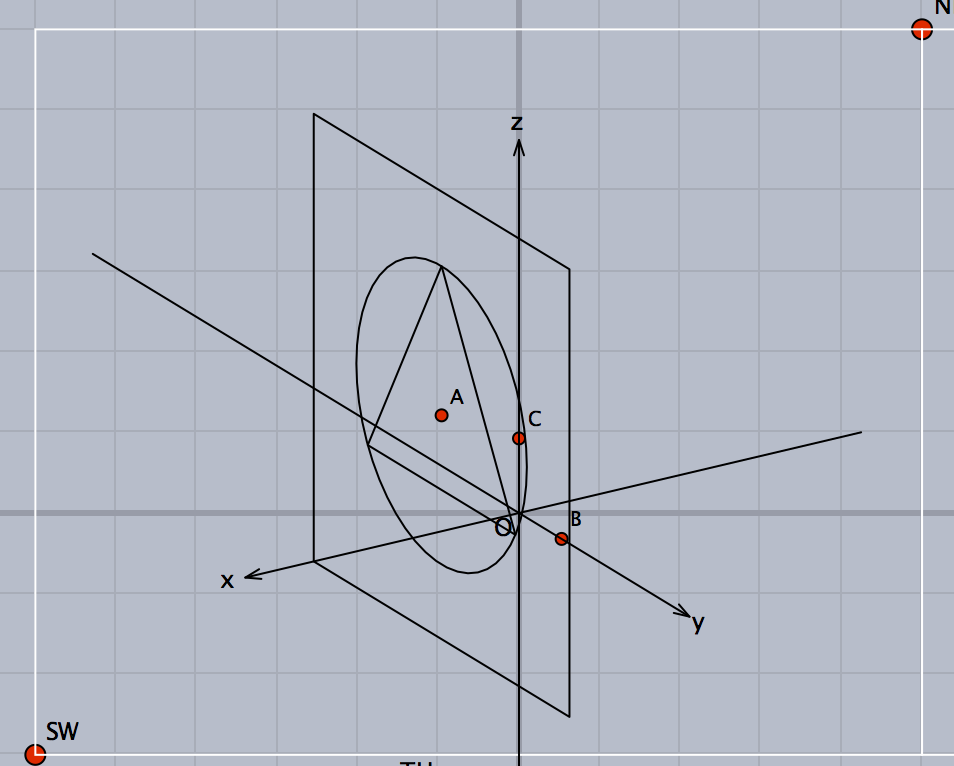
\includegraphics[bb=0 0 954 766 , width=6cm]{Fig3d/embed03.png}\\

この場合,点B,Cの座標がそのまま基本ベクトルとなっているが,原点Aに対して描画平面上にはB,Cがないので図がわかりにくい。図をわかりやすくするならば次のようにする。
\begin{verbatim}
 Putpoint3d(["A",[3,3,3],"B",[3,4,3],"C",[3,3,4]],"fix");
 Embed("1",["cr1","sg1"],"A3d+x*(B3d-A3d)+y*(C3d-A3d)","[x,y]");
\end{verbatim}

 また,平面を記述するのに,平面の原点と法線ベクトルを用いて Perpplane() を用いると,基本ベクトルが生成されるので、これを利用することができる。次のスクリプトでは,Skeletonparadata() を用いて陰線処理もしている。
\begin{verbatim}
 Xyzax3data("","x=[-5,5]","y=[-8,5]","z=[-5,5]");
 Putpoint3d(["O",[0,0,0],"P",[1,1,2]],"fix");
 Perpplane("E-F","P",P3d-O3d,"put");
 vec1=3*(E3d-P3d);
 vec2=3*(F3d-P3d);
 Putpoint3d(["A",P3d+vec1+vec2],"fix");
 Putpoint3d(["B",P3d+vec1-vec2],"fix");
 Putpoint3d(["C",P3d-vec1-vec2],"fix");
 Putpoint3d(["D",P3d-vec1+vec2],"fix");
 Spaceline([A,B,C,D,A]);
 Circledata("1",[[0,0],[2,0]],["nodisp"]);
 Listplot("1",[[0,2],[-sqrt(3),-1],[sqrt(3),-1],[0,2]],["nodisp"]);
 Embed("1",["cr1","sg1"],"P3d+x*(E3d-P3d)+y*(F3d-P3d)","[x,y]");
 Ptsize(3);
 Drawpoint(P);
 Skeletonparadata("1");
\end{verbatim}
     %%% /Users/Hannya/ketcindy/ketwork/template.tex 2016-8-18 21:20
%%% template.sce 2016-8-18 21:20
{\unitlength=8mm%
\begin{picture}%
(   9.18000,   7.71000)(  -4.79000,  -2.03000)%
\special{pn 8}%
%
\settowidth{\Width}{$x$}\setlength{\Width}{-0.5\Width}%
\settoheight{\Height}{$x$}\settodepth{\Depth}{$x$}\setlength{\Height}{-0.5\Height}\setlength{\Depth}{0.5\Depth}\addtolength{\Height}{\Depth}%
\put(-4.4289,-1.0449){\hspace*{\Width}\raisebox{\Height}{$x$}}%
%
%
\settowidth{\Width}{$y$}\setlength{\Width}{-0.5\Width}%
\settoheight{\Height}{$y$}\settodepth{\Depth}{$y$}\setlength{\Height}{-0.5\Height}\setlength{\Depth}{0.5\Depth}\addtolength{\Height}{\Depth}%
\put(2.8060,-1.7060){\hspace*{\Width}\raisebox{\Height}{$y$}}%
%
%
\settowidth{\Width}{$z$}\setlength{\Width}{-0.5\Width}%
\settoheight{\Height}{$z$}\settodepth{\Depth}{$z$}\setlength{\Height}{-0.5\Height}\setlength{\Depth}{0.5\Depth}\addtolength{\Height}{\Depth}%
\put(0.0000,4.8175){\hspace*{\Width}\raisebox{\Height}{$z$}}%
%
%
\special{pn 3}%
\special{pa -92 -427}\special{pa -99 -430}\special{pa -106 -429}\special{pa -111 -424}%
\special{pa -112 -417}\special{pa -109 -410}\special{pa -103 -407}\special{pa -95 -408}%
\special{pa -90 -413}\special{pa -89 -421}\special{pa -92 -427}\special{sh 1}\special{fp}%
\special{pn 8}%
\special{pa 1337 -315}\special{pa 811 -191}%
\special{fp}%
\special{pa 758 -179}\special{pa 380 -90}%
\special{fp}%
\special{pa 305 -72}\special{pa -311 73}%
\special{fp}%
\special{pa -385 91}\special{pa -1166 275}%
\special{fp}%
\special{pa -1219 288}\special{pa -1337 315}%
\special{fp}%
\special{pa -1332 -810}\special{pa -1019 -619}%
\special{fp}%
\special{pa -976 -593}\special{pa -742 -451}%
\special{fp}%
\special{pa -697 -424}\special{pa -581 -353}%
\special{fp}%
\special{pa -538 -327}\special{pa -306 -186}%
\special{fp}%
\special{pa -238 -144}\special{pa 78 47}%
\special{fp}%
\special{pa 130 79}\special{pa 635 386}%
\special{fp}%
\special{pa 677 412}\special{pa 833 506}%
\special{fp}%
\special{pa 0 639}\special{pa 0 418}%
\special{fp}%
\special{pa 0 369}\special{pa 0 119}%
\special{fp}%
\special{pa 0 68}\special{pa 0 -117}%
\special{fp}%
\special{pa 0 -166}\special{pa 0 -1458}%
\special{fp}%
\special{pa 993 -1126}\special{pa 645 451}\special{pa -1195 289}\special{pa -846 -1288}%
\special{pa -24 -1216}%
\special{fp}%
\special{pa 24 -1212}\special{pa 993 -1126}%
\special{fp}%
\special{pa 513 -365}\special{pa 523 -431}\special{pa 522 -497}\special{pa 513 -562}%
\special{pa 493 -625}\special{pa 464 -684}\special{pa 426 -740}\special{pa 380 -790}%
\special{pa 326 -834}\special{pa 266 -872}\special{pa 199 -903}\special{pa 129 -926}%
\special{pa 54 -941}\special{pa 24 -943}%
\special{fp}%
\special{pa -24 -947}\special{pa -101 -946}\special{pa -180 -936}\special{pa -257 -918}%
\special{pa -331 -892}\special{pa -402 -859}\special{pa -468 -818}\special{pa -529 -772}%
\special{pa -582 -720}\special{pa -628 -663}\special{pa -666 -602}\special{pa -695 -538}%
\special{pa -714 -473}\special{pa -724 -406}\special{pa -724 -340}\special{pa -714 -275}%
\special{pa -695 -212}\special{pa -666 -153}\special{pa -628 -98}\special{pa -582 -48}%
\special{pa -528 -3}\special{pa -467 35}\special{pa -401 65}\special{pa -330 88}\special{pa -255 103}%
\special{pa -178 110}\special{pa -100 108}\special{pa -22 99}\special{pa 55 81}\special{pa 130 55}%
\special{pa 201 21}\special{pa 267 -19}\special{pa 327 -66}\special{pa 381 -118}\special{pa 427 -175}%
\special{pa 465 -235}\special{pa 493 -299}\special{pa 513 -365}%
\special{fp}%
\special{pa -22 -905}\special{pa -690 -202}\special{pa 372 -109}\special{pa 16 -945}%
\special{fp}%
\end{picture}}%

\begin{flushright} \hyperlink{functionlist3d}{$\Rightarrow$関数一覧}\end{flushright}


\hypertarget{intersectcrvsf}{}
\item[関数] Intersectcrvsf(name,PD,式)
\item[機能] 曲線と曲面の交点の座標を求める
\item[説明] PDは曲線のプロットデータ。式は曲面の式。\\
 \\
【例】回転放物面と線分の交点の座標を表示する。曲面は表示されていなくてもよい。
\begin{verbatim}
Putpoint3d(["A",[0,-3,0],"B",[0,3,2]],"fix");
Spaceline([A,B]);
fd=["z=4-(x^2+y^2)","x=R*cos(T)","y=R*sin(T)","R=[0,2]","T=[0,2*pi]","e"];
println("Intersect="+Intersectcrvsf("1","AB3d",fd));
\end{verbatim}
実行すると,コンソールに\\
  \verb|Intersect=[[0,-1.91,0.36,1.18],[0,1.57,1.52,1.76]] |
と表示される。\\

\hypertarget{intersectsgpL}{}
\item[関数] IntersectsgpL(点名,線分,面,描画方法)
\item[機能] 空間の線分と平面の交点を作図する
\item[説明] 引数の線分は線分の端点を "A-B" の形もしくは座標のリスト形で与える。\\
 引数の面は,面内の3点を "C-D-E" の形もしくは座標のリストで与える。\\
 描画方法は,"put" または "draw" で,描画方法を指定しない場合は "draw" と同じ。"draw"では交点が緑の点で表示されるだけで,幾何点はできない。"put" では幾何点を作る。\\
 \\
【例】座標のリストで与える記述例\\
 \verb|IntersectsgpL("P",[p1,p2],[p3,p4,p5],"draw");| \\
 \\
【例】立方体を平面で切った図を描く。\\
  いろいろな手順が考えられるが,ここでは次の手順で描く。\\
 (1) 立方体の頂点をとる。1辺の長さをHnとする。\\
  ここでは軸上の点はPutaxes3d()でとる。\\
(2) 切断面を決める点E,F,Gを辺上の自由点としてPutonseg3d()でとる。\\
(3) E,F,Gを通る平面と,辺AC,DYとの交点をとり,M,Nとする。\\
(4) 全体を多面体として面データを作って描画する。
\begin{verbatim}
 Hn=3;
 Putaxes3d(Hn);
 Putpoint3d("A",[Hn,Hn,0],"fix");
 Putpoint3d("B",[Hn,0,Hn],"fix");
 Putpoint3d("C",[Hn,Hn,Hn],"fix");
 Putpoint3d("D",[0,Hn,Hn],"fix");
 Putonseg3d("E",X,B); 
 Putonseg3d("F",Z,B); 
 Putonseg3d("G",Z,D); 
 IntersectsgpL("M","A-C","E-F-G","put"); 
 IntersectsgpL("N","D-Y","E-F-G","put"); 
 phd=Concatobj([[O,X,A,Y],[X,A,M,E],[A,Y,N,M],[Y,N,G,Z,O],
   [O,Z,F,E,X],[Z,F,G],[E,M,N,G,F]]);
 VertexEdgeFace("1",phd,["Edg=nogeo"]);
 Nohiddenbyfaces("1","phf3d1"); 
\end{verbatim}
Cinderellaの描画面はつぎのようになる。点E,F,Gをドラッグして,適当な位置の断面にできる。ただし,M,Nは辺上にあることが条件である。
\\
 \\
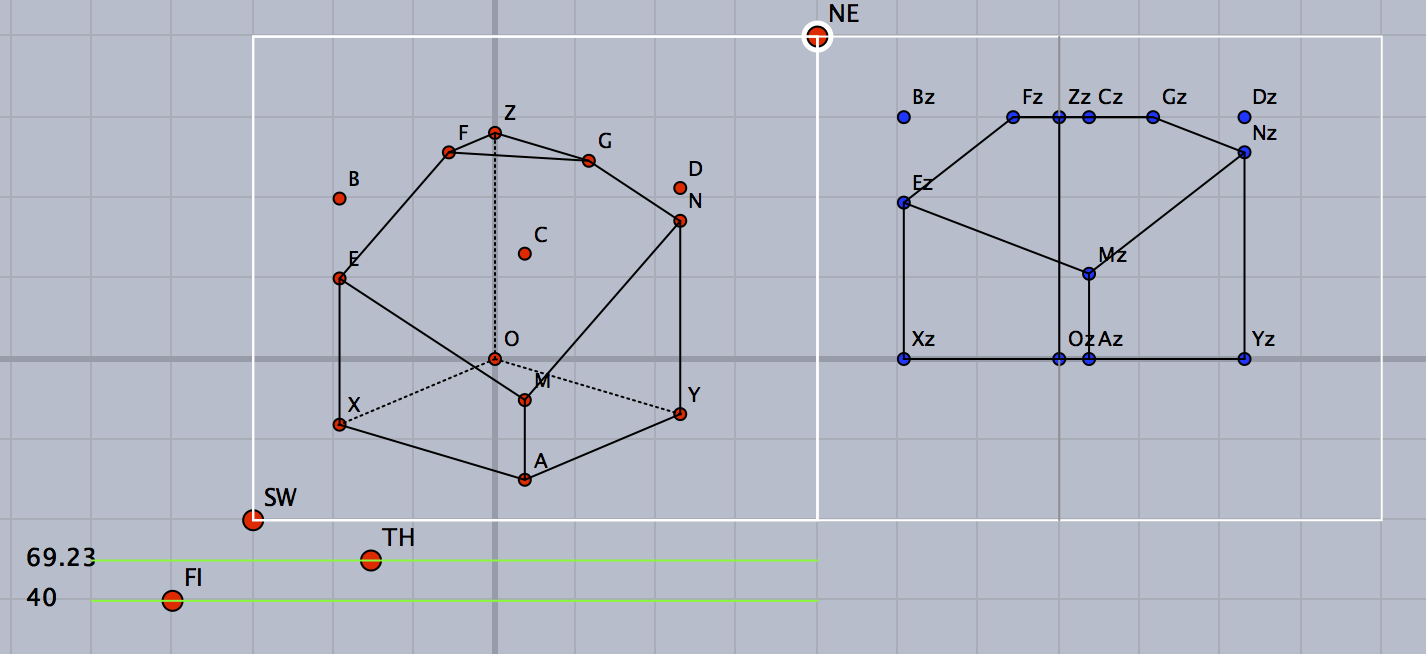
\includegraphics[bb=0 0 1426 654 , width=12cm]{Fig3d/IntersectsgpL0.png}\\

できた図は下図左。これに,次のスクリプトを追加すれば,断面上方の立方体の各辺も点線で描かれる。(下図右)
\begin{verbatim}
 Spaceline([E,B,F],["do"]);
 Spaceline([B,C,M],["do"]);
 Spaceline([C,D,N],["do"]);
 Spaceline([D,G],["do"]);
\end{verbatim}
%%% /Users/Hannya/ketcindy/ketwork/template.tex 2016-8-9 13:39
%%% template.sce 2016-8-9 13:39
{\unitlength=8mm%
\begin{picture}%
(   7.00000,   6.00000)(  -3.00000,  -2.00000)%
\special{pn 8}%
%
\special{pn 8}%
\special{pa 4 -2}\special{pa -4 2}\special{fp}\special{pa -32 14}\special{pa -39 17}\special{fp}%
\special{pa -68 29}\special{pa -75 32}\special{fp}\special{pa -103 44}\special{pa -111 47}\special{fp}%
\special{pa -139 59}\special{pa -147 62}\special{fp}\special{pa -175 74}\special{pa -182 77}\special{fp}%
\special{pa -211 89}\special{pa -218 92}\special{fp}\special{pa -246 104}\special{pa -254 107}\special{fp}%
\special{pa -282 119}\special{pa -290 122}\special{fp}\special{pa -318 134}\special{pa -325 137}\special{fp}%
\special{pa -354 149}\special{pa -361 153}\special{fp}\special{pa -389 164}\special{pa -397 168}\special{fp}%
\special{pa -425 180}\special{pa -432 183}\special{fp}\special{pa -461 195}\special{pa -468 198}\special{fp}%
\special{pa -496 210}\special{pa -504 213}\special{fp}\special{pa -532 225}\special{pa -540 228}\special{fp}%
\special{pa -568 240}\special{pa -575 243}\special{fp}\special{pa -604 255}\special{pa -611 258}\special{fp}%
\special{pn 8}%
\special{pa -607 257}\special{pa 116 472}%
\special{fp}%
\special{pa 116 472}\special{pa 724 215}%
\special{fp}%
\special{pn 8}%
\special{pa -4 -1}\special{pa 4 1}\special{fp}\special{pa 34 10}\special{pa 42 12}\special{fp}%
\special{pa 72 22}\special{pa 80 24}\special{fp}\special{pa 110 33}\special{pa 118 35}\special{fp}%
\special{pa 149 44}\special{pa 156 46}\special{fp}\special{pa 187 56}\special{pa 194 58}\special{fp}%
\special{pa 225 67}\special{pa 232 69}\special{fp}\special{pa 263 78}\special{pa 271 80}\special{fp}%
\special{pa 301 90}\special{pa 309 92}\special{fp}\special{pa 339 101}\special{pa 347 103}\special{fp}%
\special{pa 377 112}\special{pa 385 114}\special{fp}\special{pa 415 124}\special{pa 423 126}\special{fp}%
\special{pa 453 135}\special{pa 461 137}\special{fp}\special{pa 491 146}\special{pa 499 148}\special{fp}%
\special{pa 530 158}\special{pa 537 160}\special{fp}\special{pa 568 169}\special{pa 575 171}\special{fp}%
\special{pa 606 180}\special{pa 613 182}\special{fp}\special{pa 644 192}\special{pa 651 194}\special{fp}%
\special{pa 682 203}\special{pa 690 205}\special{fp}\special{pa 720 214}\special{pa 728 216}\special{fp}%
\special{pn 8}%
\special{pa 116 472}\special{pa 116 160}%
\special{fp}%
\special{pa 116 160}\special{pa -607 -315}%
\special{fp}%
\special{pa -607 257}\special{pa -607 -315}%
\special{fp}%
\special{pa 724 215}\special{pa 724 -539}%
\special{fp}%
\special{pa 116 160}\special{pa 724 -539}%
\special{fp}%
\special{pa 724 -539}\special{pa 367 -774}%
\special{fp}%
\special{pa 367 -774}\special{pa 0 -883}%
\special{fp}%
\special{pn 8}%
\special{pa 0 4}\special{pa 0 -4}\special{fp}\special{pa 0 -36}\special{pa 0 -44}\special{fp}%
\special{pa 0 -76}\special{pa 0 -84}\special{fp}\special{pa 0 -116}\special{pa 0 -124}\special{fp}%
\special{pa 0 -157}\special{pa 0 -165}\special{fp}\special{pa 0 -197}\special{pa 0 -205}\special{fp}%
\special{pa 0 -237}\special{pa 0 -245}\special{fp}\special{pa 0 -277}\special{pa 0 -285}\special{fp}%
\special{pa 0 -317}\special{pa 0 -325}\special{fp}\special{pa 0 -357}\special{pa 0 -365}\special{fp}%
\special{pa 0 -398}\special{pa 0 -406}\special{fp}\special{pa 0 -438}\special{pa 0 -446}\special{fp}%
\special{pa 0 -478}\special{pa 0 -486}\special{fp}\special{pa 0 -518}\special{pa 0 -526}\special{fp}%
\special{pa 0 -558}\special{pa 0 -566}\special{fp}\special{pa 0 -598}\special{pa 0 -606}\special{fp}%
\special{pa 0 -639}\special{pa 0 -647}\special{fp}\special{pa 0 -679}\special{pa 0 -687}\special{fp}%
\special{pa 0 -719}\special{pa 0 -727}\special{fp}\special{pa 0 -759}\special{pa 0 -767}\special{fp}%
\special{pa 0 -799}\special{pa 0 -807}\special{fp}\special{pa 0 -839}\special{pa 0 -847}\special{fp}%
\special{pa 0 -879}\special{pa 0 -887}\special{fp}\special{pn 8}%
\special{pa 0 -883}\special{pa -180 -807}%
\special{fp}%
\special{pa -607 -315}\special{pa -180 -807}%
\special{fp}%
\special{pa 367 -774}\special{pa -180 -807}%
\special{fp}%
\end{picture}}%   %%% /Users/Hannya/ketcindy/ketwork/template.tex 2016-8-9 13:37
%%% template.sce 2016-8-9 13:37
{\unitlength=8mm%
\begin{picture}%
(   7.00000,   6.00000)(  -3.00000,  -2.00000)%
\special{pn 8}%
%
\special{pn 8}%
\special{pa 4 -2}\special{pa -4 2}\special{fp}\special{pa -32 14}\special{pa -39 17}\special{fp}%
\special{pa -68 29}\special{pa -75 32}\special{fp}\special{pa -103 44}\special{pa -111 47}\special{fp}%
\special{pa -139 59}\special{pa -147 62}\special{fp}\special{pa -175 74}\special{pa -182 77}\special{fp}%
\special{pa -211 89}\special{pa -218 92}\special{fp}\special{pa -246 104}\special{pa -254 107}\special{fp}%
\special{pa -282 119}\special{pa -290 122}\special{fp}\special{pa -318 134}\special{pa -325 137}\special{fp}%
\special{pa -354 149}\special{pa -361 153}\special{fp}\special{pa -389 164}\special{pa -397 168}\special{fp}%
\special{pa -425 180}\special{pa -432 183}\special{fp}\special{pa -461 195}\special{pa -468 198}\special{fp}%
\special{pa -496 210}\special{pa -504 213}\special{fp}\special{pa -532 225}\special{pa -540 228}\special{fp}%
\special{pa -568 240}\special{pa -575 243}\special{fp}\special{pa -604 255}\special{pa -611 258}\special{fp}%
\special{pn 8}%
\special{pa -607 257}\special{pa 116 472}%
\special{fp}%
\special{pa 116 472}\special{pa 724 215}%
\special{fp}%
\special{pn 8}%
\special{pa -4 -1}\special{pa 4 1}\special{fp}\special{pa 34 10}\special{pa 42 12}\special{fp}%
\special{pa 72 22}\special{pa 80 24}\special{fp}\special{pa 110 33}\special{pa 118 35}\special{fp}%
\special{pa 149 44}\special{pa 156 46}\special{fp}\special{pa 187 56}\special{pa 194 58}\special{fp}%
\special{pa 225 67}\special{pa 232 69}\special{fp}\special{pa 263 78}\special{pa 271 80}\special{fp}%
\special{pa 301 90}\special{pa 309 92}\special{fp}\special{pa 339 101}\special{pa 347 103}\special{fp}%
\special{pa 377 112}\special{pa 385 114}\special{fp}\special{pa 415 124}\special{pa 423 126}\special{fp}%
\special{pa 453 135}\special{pa 461 137}\special{fp}\special{pa 491 146}\special{pa 499 148}\special{fp}%
\special{pa 530 158}\special{pa 537 160}\special{fp}\special{pa 568 169}\special{pa 575 171}\special{fp}%
\special{pa 606 180}\special{pa 613 182}\special{fp}\special{pa 644 192}\special{pa 651 194}\special{fp}%
\special{pa 682 203}\special{pa 690 205}\special{fp}\special{pa 720 214}\special{pa 728 216}\special{fp}%
\special{pn 8}%
\special{pa 116 472}\special{pa 116 160}%
\special{fp}%
\special{pa 116 160}\special{pa -607 -315}%
\special{fp}%
\special{pa -607 257}\special{pa -607 -315}%
\special{fp}%
\special{pa 724 215}\special{pa 724 -539}%
\special{fp}%
\special{pa 116 160}\special{pa 724 -539}%
\special{fp}%
\special{pa 724 -539}\special{pa 367 -774}%
\special{fp}%
\special{pa 367 -774}\special{pa 0 -883}%
\special{fp}%
\special{pn 8}%
\special{pa 0 4}\special{pa 0 -4}\special{fp}\special{pa 0 -36}\special{pa 0 -44}\special{fp}%
\special{pa 0 -76}\special{pa 0 -84}\special{fp}\special{pa 0 -116}\special{pa 0 -124}\special{fp}%
\special{pa 0 -157}\special{pa 0 -165}\special{fp}\special{pa 0 -197}\special{pa 0 -205}\special{fp}%
\special{pa 0 -237}\special{pa 0 -245}\special{fp}\special{pa 0 -277}\special{pa 0 -285}\special{fp}%
\special{pa 0 -317}\special{pa 0 -325}\special{fp}\special{pa 0 -357}\special{pa 0 -365}\special{fp}%
\special{pa 0 -398}\special{pa 0 -406}\special{fp}\special{pa 0 -438}\special{pa 0 -446}\special{fp}%
\special{pa 0 -478}\special{pa 0 -486}\special{fp}\special{pa 0 -518}\special{pa 0 -526}\special{fp}%
\special{pa 0 -558}\special{pa 0 -566}\special{fp}\special{pa 0 -598}\special{pa 0 -606}\special{fp}%
\special{pa 0 -639}\special{pa 0 -647}\special{fp}\special{pa 0 -679}\special{pa 0 -687}\special{fp}%
\special{pa 0 -719}\special{pa 0 -727}\special{fp}\special{pa 0 -759}\special{pa 0 -767}\special{fp}%
\special{pa 0 -799}\special{pa 0 -807}\special{fp}\special{pa 0 -839}\special{pa 0 -847}\special{fp}%
\special{pa 0 -879}\special{pa 0 -887}\special{fp}\special{pn 8}%
\special{pa 0 -883}\special{pa -180 -807}%
\special{fp}%
\special{pa -607 -315}\special{pa -180 -807}%
\special{fp}%
\special{pa 367 -774}\special{pa -180 -807}%
\special{fp}%
\special{pn 8}%
\special{pa -607 -311}\special{pa -607 -319}\special{fp}\special{pa -607 -349}\special{pa -607 -357}\special{fp}%
\special{pa -607 -388}\special{pa -607 -396}\special{fp}\special{pa -607 -427}\special{pa -607 -435}\special{fp}%
\special{pa -607 -466}\special{pa -607 -474}\special{fp}\special{pa -607 -505}\special{pa -607 -513}\special{fp}%
\special{pa -607 -543}\special{pa -607 -551}\special{fp}\special{pa -607 -582}\special{pa -607 -590}\special{fp}%
\special{pa -609 -622}\special{pa -605 -628}\special{fp}\special{pa -577 -640}\special{pa -570 -643}\special{fp}%
\special{pa -541 -655}\special{pa -534 -658}\special{fp}\special{pa -505 -670}\special{pa -498 -673}\special{fp}%
\special{pa -470 -685}\special{pa -462 -688}\special{fp}\special{pa -434 -700}\special{pa -427 -703}\special{fp}%
\special{pa -398 -715}\special{pa -391 -718}\special{fp}\special{pa -363 -730}\special{pa -355 -733}\special{fp}%
\special{pa -327 -745}\special{pa -319 -749}\special{fp}\special{pa -291 -761}\special{pa -284 -764}\special{fp}%
\special{pa -255 -776}\special{pa -248 -779}\special{fp}\special{pa -220 -791}\special{pa -212 -794}\special{fp}%
\special{pa -184 -806}\special{pa -176 -809}\special{fp}\special{pn 8}%
\special{pn 8}%
\special{pa -611 -628}\special{pa -604 -626}\special{fp}\special{pa -574 -617}\special{pa -566 -615}\special{fp}%
\special{pa -536 -606}\special{pa -529 -603}\special{fp}\special{pa -499 -595}\special{pa -491 -592}\special{fp}%
\special{pa -462 -584}\special{pa -454 -581}\special{fp}\special{pa -424 -572}\special{pa -417 -570}\special{fp}%
\special{pa -387 -561}\special{pa -379 -559}\special{fp}\special{pa -349 -550}\special{pa -342 -548}\special{fp}%
\special{pa -312 -539}\special{pa -304 -537}\special{fp}\special{pa -275 -528}\special{pa -267 -526}\special{fp}%
\special{pa -237 -517}\special{pa -230 -514}\special{fp}\special{pa -200 -506}\special{pa -192 -503}\special{fp}%
\special{pa -162 -495}\special{pa -155 -492}\special{fp}\special{pa -125 -483}\special{pa -117 -481}\special{fp}%
\special{pa -88 -472}\special{pa -80 -470}\special{fp}\special{pa -50 -461}\special{pa -43 -459}\special{fp}%
\special{pa -13 -450}\special{pa -5 -448}\special{fp}\special{pa 25 -439}\special{pa 32 -437}\special{fp}%
\special{pa 62 -428}\special{pa 70 -425}\special{fp}\special{pa 100 -418}\special{pa 106 -413}\special{fp}%
\special{pa 116 -390}\special{pa 117 -382}\special{fp}\special{pa 116 -351}\special{pa 116 -343}\special{fp}%
\special{pa 116 -312}\special{pa 116 -304}\special{fp}\special{pa 116 -273}\special{pa 116 -265}\special{fp}%
\special{pa 116 -234}\special{pa 116 -226}\special{fp}\special{pa 116 -195}\special{pa 116 -187}\special{fp}%
\special{pa 116 -156}\special{pa 116 -148}\special{fp}\special{pa 116 -117}\special{pa 116 -109}\special{fp}%
\special{pa 116 -78}\special{pa 116 -70}\special{fp}\special{pa 116 -39}\special{pa 116 -31}\special{fp}%
\special{pa 116 0}\special{pa 116 8}\special{fp}\special{pa 116 39}\special{pa 116 47}\special{fp}%
\special{pa 116 78}\special{pa 116 86}\special{fp}\special{pa 116 117}\special{pa 116 125}\special{fp}%
\special{pa 116 156}\special{pa 116 164}\special{fp}\special{pn 8}%
\special{pn 8}%
\special{pa 113 -410}\special{pa 120 -413}\special{fp}\special{pa 149 -425}\special{pa 156 -428}\special{fp}%
\special{pa 185 -441}\special{pa 193 -444}\special{fp}\special{pa 222 -456}\special{pa 229 -459}\special{fp}%
\special{pa 258 -471}\special{pa 265 -474}\special{fp}\special{pa 294 -487}\special{pa 302 -490}\special{fp}%
\special{pa 331 -502}\special{pa 338 -505}\special{fp}\special{pa 367 -517}\special{pa 374 -521}\special{fp}%
\special{pa 403 -533}\special{pa 411 -536}\special{fp}\special{pa 440 -548}\special{pa 447 -551}\special{fp}%
\special{pa 476 -564}\special{pa 484 -567}\special{fp}\special{pa 512 -579}\special{pa 520 -582}\special{fp}%
\special{pa 549 -594}\special{pa 556 -597}\special{fp}\special{pa 585 -610}\special{pa 593 -613}\special{fp}%
\special{pa 621 -625}\special{pa 629 -628}\special{fp}\special{pa 658 -640}\special{pa 665 -643}\special{fp}%
\special{pa 694 -656}\special{pa 702 -658}\special{fp}\special{pa 721 -660}\special{pa 727 -654}\special{fp}%
\special{pa 724 -621}\special{pa 724 -613}\special{fp}\special{pa 724 -582}\special{pa 724 -574}\special{fp}%
\special{pa 724 -543}\special{pa 724 -535}\special{fp}\special{pn 8}%
\special{pn 8}%
\special{pa 728 -667}\special{pa 720 -669}\special{fp}\special{pa 688 -679}\special{pa 680 -681}\special{fp}%
\special{pa 648 -691}\special{pa 641 -693}\special{fp}\special{pa 609 -702}\special{pa 601 -705}\special{fp}%
\special{pa 569 -714}\special{pa 561 -717}\special{fp}\special{pa 529 -726}\special{pa 522 -728}\special{fp}%
\special{pa 490 -738}\special{pa 482 -740}\special{fp}\special{pa 450 -750}\special{pa 442 -752}\special{fp}%
\special{pa 410 -761}\special{pa 403 -764}\special{fp}\special{pa 371 -773}\special{pa 363 -776}\special{fp}%
\special{pn 8}%
\end{picture}}%

\begin{flushright} \hyperlink{functionlist3d}{$\Rightarrow$関数一覧}\end{flushright}

\hypertarget{invparapt}{}
\item[関数] Invparapt(座標,PD)
\item[機能] 描画面上の座標に対応する曲線上の点の座標を返す
\item[説明] Cinderellaの描画面上の座標を与えて,それに対応する曲線上の3次元座標を返す。
\\
空間内の曲線を作図すると,曲線の空間内のプロットデータとともに,描画面上に描くためのプロットデータも作られる。これを利用すると,描画面上の位置から曲線上の座標を求めることができる。\\
 \\
【例】螺旋と線分を描いたとき,描画面上での交点(空間内の交点ではない)に対応する螺旋上の点の座標を求め部分曲線を描く。\\
\begin{verbatim}
 Spaceline("1",[[-1,-1,-1],[1,2,3]]);
 Spacecurve("1","[2*cos(t),2*sin(t),0.2*t]","t=[0,4*pi]",["do"]);
 tmp=Intersectcrvs("sl2d1","sc2d1");
 p1=Invparapt(tmp_1,"sc3d1");
 p2=Invparapt(tmp_2,"sc3d1");
 Partcrv3d("1",p1,p2,"sc3d1"); 
\end{verbatim}
        %%% /Users/Hannya/ketcindy/ketwork/template.tex 2016-8-23 9:12
%%% template.sce 2016-8-23 9:12
{\unitlength=8mm%
\begin{picture}%
(   7.55000,   6.27000)(  -3.75000,  -1.85000)%
\special{pn 8}%
%
\settowidth{\Width}{$x$}\setlength{\Width}{-0.5\Width}%
\settoheight{\Height}{$x$}\settodepth{\Depth}{$x$}\setlength{\Height}{-0.5\Height}\setlength{\Depth}{0.5\Depth}\addtolength{\Height}{\Depth}%
\put(-3.1557,-0.9707){\hspace*{\Width}\raisebox{\Height}{$x$}}%
%
%
\settowidth{\Width}{$y$}\setlength{\Width}{-0.5\Width}%
\settoheight{\Height}{$y$}\settodepth{\Depth}{$y$}\setlength{\Height}{-0.5\Height}\setlength{\Depth}{0.5\Depth}\addtolength{\Height}{\Depth}%
\put(3.5211,-1.3391){\hspace*{\Width}\raisebox{\Height}{$y$}}%
%
%
\settowidth{\Width}{$z$}\setlength{\Width}{-0.5\Width}%
\settoheight{\Height}{$z$}\settodepth{\Depth}{$z$}\setlength{\Height}{-0.5\Height}\setlength{\Depth}{0.5\Depth}\addtolength{\Height}{\Depth}%
\put(0.0000,3.9488){\hspace*{\Width}\raisebox{\Height}{$z$}}%
%
%
\special{pa 1171 -360}\special{pa -937 288}%
\special{fp}%
\special{pa -1053 -400}\special{pa 1053 400}%
\special{fp}%
\special{pa 0 583}\special{pa 0 -1184}%
\special{fp}%
\special{pa 24 144}\special{pa 187 -656}%
\special{fp}%
\special{pn 8}%
\special{pa -472 143}\special{pa -464 145}\special{fp}\special{pa -434 150}\special{pa -426 151}\special{fp}%
\special{pa -395 157}\special{pa -387 158}\special{fp}\special{pa -356 163}\special{pa -348 164}\special{fp}%
\special{pa -317 167}\special{pa -309 167}\special{fp}\special{pa -278 169}\special{pa -270 170}\special{fp}%
\special{pa -239 172}\special{pa -231 172}\special{fp}\special{pa -199 173}\special{pa -191 173}\special{fp}%
\special{pa -160 173}\special{pa -152 172}\special{fp}\special{pa -121 172}\special{pa -113 171}\special{fp}%
\special{pa -82 171}\special{pa -74 170}\special{fp}\special{pa -42 169}\special{pa -34 168}\special{fp}%
\special{pa -3 165}\special{pa 5 164}\special{fp}\special{pa 36 160}\special{pa 44 160}\special{fp}%
\special{pa 75 156}\special{pa 83 155}\special{fp}\special{pa 114 151}\special{pa 122 150}\special{fp}%
\special{pa 152 143}\special{pa 160 142}\special{fp}\special{pa 191 136}\special{pa 199 134}\special{fp}%
\special{pa 229 128}\special{pa 237 126}\special{fp}\special{pa 267 119}\special{pa 275 117}\special{fp}%
\special{pa 305 107}\special{pa 312 105}\special{fp}\special{pa 342 95}\special{pa 350 93}\special{fp}%
\special{pa 380 83}\special{pa 387 81}\special{fp}\special{pa 416 68}\special{pa 423 64}\special{fp}%
\special{pa 451 51}\special{pa 458 47}\special{fp}\special{pa 487 34}\special{pa 493 30}\special{fp}%
\special{pa 519 12}\special{pa 526 8}\special{fp}\special{pa 550 -12}\special{pa 556 -17}\special{fp}%
\special{pa 581 -36}\special{pa 586 -42}\special{fp}\special{pa 602 -69}\special{pa 606 -76}\special{fp}%
\special{pa 622 -103}\special{pa 624 -110}\special{fp}\special{pa 625 -142}\special{pa 625 -150}\special{fp}%
\special{pa 621 -179}\special{pa 619 -187}\special{fp}\special{pa 604 -215}\special{pa 599 -221}\special{fp}%
\special{pa 581 -246}\special{pa 576 -252}\special{fp}\special{pa 552 -272}\special{pa 546 -277}\special{fp}%
\special{pa 522 -298}\special{pa 516 -302}\special{fp}\special{pa 488 -317}\special{pa 481 -321}\special{fp}%
\special{pa 453 -335}\special{pa 446 -339}\special{fp}\special{pa 418 -353}\special{pa 411 -357}\special{fp}%
\special{pa 381 -367}\special{pa 374 -369}\special{fp}\special{pa 344 -379}\special{pa 337 -382}\special{fp}%
\special{pa 307 -392}\special{pa 300 -395}\special{fp}\special{pa 270 -403}\special{pa 262 -405}\special{fp}%
\special{pa 231 -412}\special{pa 223 -414}\special{fp}\special{pa 193 -420}\special{pa 185 -422}\special{fp}%
\special{pa 155 -429}\special{pa 147 -430}\special{fp}\special{pa 116 -436}\special{pa 108 -437}\special{fp}%
\special{pa 77 -441}\special{pa 69 -442}\special{fp}\special{pa 38 -445}\special{pa 30 -446}\special{fp}%
\special{pa -1 -450}\special{pa -9 -451}\special{fp}\special{pa -40 -454}\special{pa -48 -454}\special{fp}%
\special{pa -79 -455}\special{pa -87 -456}\special{fp}\special{pa -119 -457}\special{pa -127 -457}\special{fp}%
\special{pa -158 -458}\special{pa -166 -459}\special{fp}\special{pa -197 -458}\special{pa -205 -458}\special{fp}%
\special{pa -236 -457}\special{pa -244 -456}\special{fp}\special{pa -276 -455}\special{pa -284 -454}\special{fp}%
\special{pa -315 -453}\special{pa -323 -452}\special{fp}\special{pa -354 -448}\special{pa -362 -447}\special{fp}%
\special{pa -393 -442}\special{pa -401 -441}\special{fp}\special{pa -432 -436}\special{pa -439 -435}\special{fp}%
\special{pa -470 -428}\special{pa -477 -425}\special{fp}\special{pa -507 -417}\special{pa -515 -414}\special{fp}%
\special{pa -545 -405}\special{pa -552 -402}\special{fp}\special{pa -579 -386}\special{pa -586 -382}\special{fp}%
\special{pa -610 -364}\special{pa -615 -357}\special{fp}\special{pa -627 -330}\special{pa -627 -322}\special{fp}%
\special{pa -613 -294}\special{pa -608 -288}\special{fp}\special{pa -581 -272}\special{pa -574 -268}\special{fp}%
\special{pa -547 -254}\special{pa -539 -251}\special{fp}\special{pa -509 -241}\special{pa -502 -239}\special{fp}%
\special{pa -472 -229}\special{pa -464 -227}\special{fp}\special{pa -434 -222}\special{pa -426 -221}\special{fp}%
\special{pa -395 -215}\special{pa -387 -214}\special{fp}\special{pa -356 -208}\special{pa -348 -208}\special{fp}%
\special{pa -317 -205}\special{pa -309 -205}\special{fp}\special{pa -278 -203}\special{pa -270 -202}\special{fp}%
\special{pa -239 -200}\special{pa -231 -200}\special{fp}\special{pa -199 -199}\special{pa -191 -199}\special{fp}%
\special{pa -160 -199}\special{pa -152 -200}\special{fp}\special{pa -121 -200}\special{pa -113 -200}\special{fp}%
\special{pa -82 -201}\special{pa -74 -201}\special{fp}\special{pa -42 -203}\special{pa -34 -204}\special{fp}%
\special{pa -3 -207}\special{pa 5 -208}\special{fp}\special{pa 36 -211}\special{pa 44 -212}\special{fp}%
\special{pa 75 -216}\special{pa 83 -217}\special{fp}\special{pa 114 -221}\special{pa 122 -222}\special{fp}%
\special{pa 152 -229}\special{pa 160 -230}\special{fp}\special{pa 191 -236}\special{pa 199 -238}\special{fp}%
\special{pa 229 -244}\special{pa 237 -246}\special{fp}\special{pa 267 -253}\special{pa 275 -255}\special{fp}%
\special{pa 305 -265}\special{pa 312 -267}\special{fp}\special{pa 342 -277}\special{pa 350 -279}\special{fp}%
\special{pa 380 -288}\special{pa 387 -291}\special{fp}\special{pa 416 -304}\special{pa 423 -308}\special{fp}%
\special{pa 451 -321}\special{pa 458 -325}\special{fp}\special{pa 487 -338}\special{pa 493 -342}\special{fp}%
\special{pa 519 -360}\special{pa 526 -364}\special{fp}\special{pa 550 -384}\special{pa 556 -389}\special{fp}%
\special{pa 581 -408}\special{pa 586 -414}\special{fp}\special{pa 602 -441}\special{pa 606 -448}\special{fp}%
\special{pa 622 -474}\special{pa 624 -482}\special{fp}\special{pa 625 -514}\special{pa 625 -522}\special{fp}%
\special{pa 621 -551}\special{pa 619 -559}\special{fp}\special{pa 604 -586}\special{pa 599 -593}\special{fp}%
\special{pa 581 -618}\special{pa 576 -624}\special{fp}\special{pa 552 -644}\special{pa 546 -649}\special{fp}%
\special{pa 522 -670}\special{pa 516 -674}\special{fp}\special{pa 488 -689}\special{pa 481 -692}\special{fp}%
\special{pa 453 -707}\special{pa 446 -711}\special{fp}\special{pa 418 -725}\special{pa 411 -728}\special{fp}%
\special{pa 381 -739}\special{pa 374 -741}\special{fp}\special{pa 344 -751}\special{pa 337 -754}\special{fp}%
\special{pa 307 -764}\special{pa 300 -767}\special{fp}\special{pa 270 -775}\special{pa 262 -777}\special{fp}%
\special{pa 231 -784}\special{pa 223 -786}\special{fp}\special{pa 193 -792}\special{pa 185 -794}\special{fp}%
\special{pa 155 -801}\special{pa 147 -802}\special{fp}\special{pa 116 -808}\special{pa 108 -809}\special{fp}%
\special{pa 77 -813}\special{pa 69 -813}\special{fp}\special{pa 38 -817}\special{pa 30 -818}\special{fp}%
\special{pa -1 -822}\special{pa -9 -823}\special{fp}\special{pa -40 -826}\special{pa -48 -826}\special{fp}%
\special{pa -79 -827}\special{pa -87 -828}\special{fp}\special{pa -119 -829}\special{pa -127 -829}\special{fp}%
\special{pa -158 -830}\special{pa -166 -830}\special{fp}\special{pa -197 -830}\special{pa -205 -830}\special{fp}%
\special{pa -236 -828}\special{pa -244 -828}\special{fp}\special{pa -276 -827}\special{pa -284 -826}\special{fp}%
\special{pa -315 -825}\special{pa -323 -824}\special{fp}\special{pa -354 -820}\special{pa -362 -819}\special{fp}%
\special{pa -393 -814}\special{pa -401 -813}\special{fp}\special{pa -432 -808}\special{pa -439 -807}\special{fp}%
\special{pa -470 -799}\special{pa -477 -797}\special{fp}\special{pa -507 -789}\special{pa -515 -786}\special{fp}%
\special{pa -545 -777}\special{pa -552 -774}\special{fp}\special{pa -579 -758}\special{pa -586 -754}\special{fp}%
\special{pa -610 -735}\special{pa -615 -729}\special{fp}\special{pa -627 -702}\special{pa -627 -694}\special{fp}%
\special{pa -613 -666}\special{pa -608 -660}\special{fp}\special{pa -581 -644}\special{pa -574 -640}\special{fp}%
\special{pa -547 -626}\special{pa -539 -623}\special{fp}\special{pa -509 -613}\special{pa -502 -611}\special{fp}%
\special{pa -472 -601}\special{pa -465 -599}\special{fp}\special{pn 8}%
\special{pa 140 -432}\special{pa 131 -433}\special{pa -27 -452}\special{pa -182 -458}%
\special{pa -326 -450}\special{pa -452 -435}\special{pa -545 -406}\special{pa -607 -372}%
\special{pa -630 -333}\special{pa -612 -294}\special{pa -560 -258}\special{pa -468 -229}%
\special{pa -349 -208}\special{pa -208 -200}\special{pa -53 -202}\special{pa 96 -220}%
\special{fp}%
\end{picture}}%\\
ここで,sl2d1,sc2d1 は線分と螺旋の描画面上での(平面の)プロットデータである。Intersectcrvs() で平面上の交点の座標(複数あるのでリストが返る)を求め,Invparapt() で対応する螺旋上の点の座標を求めて部分曲線を描いている。実際に交わる点での部分曲線ではないことに注意。\\
 \\

\hypertarget{mkbezierptcrv3d}{}
\item[関数] Mkbezierptcrv3d(点リスト)
\item[機能] 制御点を自動的にとる空間ベジェ曲線
\item[説明] リストで与えた点に対し,制御点を自動的に生成してベジェ曲線を描く。\\
 制御点は,2つの点に対して,その点を端点とする線分上に2つ作られる。これを適宜移動して任意の曲線にすることができる。\hyperlink{bezier3d}{空間ベジェ曲線 Bezier3d()} を参照のこと。\\
 \\
【例】\verb|Mkbezierptcrv3d(["A","B","C","D"]);|\\
  線分AB上に2点a1p,a2p,線分BC上に2点a2p,a2q,線分CD上に2点a3p,a3qができる。\\

\begin{flushright} \hyperlink{functionlist3d}{$\Rightarrow$関数一覧}\end{flushright}

\hypertarget{nohiddenbyfaces}{}
\item[関数] Nohiddenbyfaces(name,PD1,PD2,option1,option2)
\item[機能] 面に対し曲線を陰線処理する
\item[説明] PD2で与えられた面に対し,曲線PD1の面に隠れている部分を陰線処理する。\\
引数PD1を省略するとすべての曲線が対象となる。陰線処理された線は初期設定では点線で表される。この線種はoption2で変更できる。たとえば,["da"] とすると破線になる。option1は曲線全体のoptionであるので,option2 だけを指定する場合は,option1 として空リスト[ ] が必要である。\\
 \\
【例】座標平面上に正四面体を描き,各軸と正四面体の辺を陰線処理する。(下図左)
\begin{verbatim}
Xyzax3data("","x=[-5,5]","y=[-5,5]","z=[-5,4]");
Putpoint3d("A",2*[-1,-1/sqrt(3),0],"fix");
Putpoint3d("B",2*[1,-1/sqrt(3),0],"fix");
Putpoint3d("C",2*[0,sqrt(3)-1/sqrt(3),0],"fix");
Putpoint3d("D",2*[0,0,sqrt(3)],"fix");
phd=Concatobj([[A,B,C],[A,B,D],[A,C,D],[B,C,D]]);
VertexEdgeFace("1",phd,["Edg=nogeo"]);
Nohiddenbyfaces("1","phf3d1"); 
\end{verbatim}

 \verb|VertexEdgeFace("1",phd,["Edg=nogeo"]);| によって,辺,頂点,面のプロットデータが作られる。\verb|phf3d1| は,面のプロットデータである。\\
 ここで,\verb|Nohiddenbyfaces("1","phe3d1","phf3d1",["dr,2"],["da"]); | とすると,座標軸は陰線処理されず,正四面体の辺(\verb|phe3d1|)だけが陰線処理されて破線で描かれる。四面体は太く描かれる。(下図右)\\
 \\
 %%% /Users/Hannya/ketcindy/ketwork/template.tex 2016-8-9 10:45
%%% template.sce 2016-8-9 10:45
{\unitlength=6mm%
\begin{picture}%
(   9.37000,   7.04000)(  -5.00000,  -2.00000)%
\special{pn 8}%
%
\settowidth{\Width}{$x$}\setlength{\Width}{-0.5\Width}%
\settoheight{\Height}{$x$}\settodepth{\Depth}{$x$}\setlength{\Height}{-0.5\Height}\setlength{\Depth}{0.5\Depth}\addtolength{\Height}{\Depth}%
\put(-3.3890,-1.4320){\hspace*{\Width}\raisebox{\Height}{$x$}}%
%
%
\settowidth{\Width}{$y$}\setlength{\Width}{-0.5\Width}%
\settoheight{\Height}{$y$}\settodepth{\Depth}{$y$}\setlength{\Height}{-0.5\Height}\setlength{\Depth}{0.5\Depth}\addtolength{\Height}{\Depth}%
\put(4.0123,-1.1937){\hspace*{\Width}\raisebox{\Height}{$y$}}%
%
%
\settowidth{\Width}{$z$}\setlength{\Width}{-0.5\Width}%
\settoheight{\Height}{$z$}\settodepth{\Depth}{$z$}\setlength{\Height}{-0.5\Height}\setlength{\Depth}{0.5\Depth}\addtolength{\Height}{\Depth}%
\put(0.0000,4.8652){\hspace*{\Width}\raisebox{\Height}{$z$}}%
%
%
\special{pa 759 -321}\special{pa 301 -127}%
\special{fp}%
\special{pa -202 85}\special{pa -759 321}%
\special{fp}%
\special{pn 8}%
\special{pa 304 -129}\special{pa 297 -125}\special{fp}\special{pa 268 -113}\special{pa 261 -110}\special{fp}%
\special{pa 233 -98}\special{pa 225 -95}\special{fp}\special{pa 197 -83}\special{pa 189 -80}\special{fp}%
\special{pa 161 -68}\special{pa 153 -65}\special{fp}\special{pa 125 -53}\special{pa 117 -50}\special{fp}%
\special{pa 89 -38}\special{pa 82 -34}\special{fp}\special{pa 53 -22}\special{pa 46 -19}\special{fp}%
\special{pa 17 -7}\special{pa 10 -4}\special{fp}\special{pa -19 8}\special{pa -26 11}\special{fp}%
\special{pa -55 23}\special{pa -62 26}\special{fp}\special{pa -91 38}\special{pa -98 41}\special{fp}%
\special{pa -126 53}\special{pa -134 57}\special{fp}\special{pa -162 69}\special{pa -170 72}\special{fp}%
\special{pa -198 84}\special{pa -206 87}\special{fp}\special{pn 8}%
\special{pa -905 -269}\special{pa -398 -118}%
\special{fp}%
\special{pa 418 124}\special{pa 905 269}%
\special{fp}%
\special{pn 8}%
\special{pa -402 -120}\special{pa -394 -117}\special{fp}\special{pa -365 -109}\special{pa -357 -106}\special{fp}%
\special{pa -328 -98}\special{pa -320 -95}\special{fp}\special{pa -291 -86}\special{pa -283 -84}\special{fp}%
\special{pa -254 -75}\special{pa -246 -73}\special{fp}\special{pa -216 -64}\special{pa -209 -62}\special{fp}%
\special{pa -179 -53}\special{pa -172 -51}\special{fp}\special{pa -142 -42}\special{pa -135 -40}\special{fp}%
\special{pa -105 -31}\special{pa -98 -29}\special{fp}\special{pa -68 -20}\special{pa -60 -18}\special{fp}%
\special{pa -31 -9}\special{pa -23 -7}\special{fp}\special{pa 6 2}\special{pa 14 4}\special{fp}%
\special{pa 43 13}\special{pa 51 15}\special{fp}\special{pa 80 24}\special{pa 88 26}\special{fp}%
\special{pa 117 35}\special{pa 125 37}\special{fp}\special{pa 155 46}\special{pa 162 48}\special{fp}%
\special{pa 192 57}\special{pa 199 59}\special{fp}\special{pa 229 68}\special{pa 236 70}\special{fp}%
\special{pa 266 79}\special{pa 273 81}\special{fp}\special{pa 303 90}\special{pa 311 92}\special{fp}%
\special{pa 340 101}\special{pa 348 103}\special{fp}\special{pa 377 112}\special{pa 385 114}\special{fp}%
\special{pa 414 123}\special{pa 422 125}\special{fp}\special{pn 8}%
\special{pa 0 472}\special{pa 0 97}%
\special{fp}%
\special{pa 0 -764}\special{pa 0 -1104}%
\special{fp}%
\special{pn 8}%
\special{pa 0 101}\special{pa 0 93}\special{fp}\special{pa 0 62}\special{pa 0 54}\special{fp}%
\special{pa 0 23}\special{pa 0 15}\special{fp}\special{pa 0 -16}\special{pa 0 -24}\special{fp}%
\special{pa 0 -55}\special{pa 0 -63}\special{fp}\special{pa 0 -95}\special{pa 0 -103}\special{fp}%
\special{pa 0 -134}\special{pa 0 -142}\special{fp}\special{pa 0 -173}\special{pa 0 -181}\special{fp}%
\special{pa 0 -212}\special{pa 0 -220}\special{fp}\special{pa 0 -251}\special{pa 0 -259}\special{fp}%
\special{pa 0 -290}\special{pa 0 -298}\special{fp}\special{pa 0 -330}\special{pa 0 -338}\special{fp}%
\special{pa 0 -369}\special{pa 0 -377}\special{fp}\special{pa 0 -408}\special{pa 0 -416}\special{fp}%
\special{pa 0 -447}\special{pa 0 -455}\special{fp}\special{pa 0 -486}\special{pa 0 -494}\special{fp}%
\special{pa 0 -525}\special{pa 0 -533}\special{fp}\special{pa 0 -564}\special{pa 0 -572}\special{fp}%
\special{pa 0 -604}\special{pa 0 -612}\special{fp}\special{pa 0 -643}\special{pa 0 -651}\special{fp}%
\special{pa 0 -682}\special{pa 0 -690}\special{fp}\special{pa 0 -721}\special{pa 0 -729}\special{fp}%
\special{pa 0 -760}\special{pa 0 -768}\special{fp}\special{pn 8}%
\special{pn 8}%
\special{pa 99 -192}\special{pa 92 -189}\special{fp}\special{pa 64 -177}\special{pa 56 -174}\special{fp}%
\special{pa 28 -162}\special{pa 20 -158}\special{fp}\special{pa -8 -146}\special{pa -15 -143}\special{fp}%
\special{pa -44 -131}\special{pa -51 -128}\special{fp}\special{pa -79 -116}\special{pa -87 -113}\special{fp}%
\special{pa -115 -101}\special{pa -122 -98}\special{fp}\special{pa -151 -86}\special{pa -158 -83}\special{fp}%
\special{pa -187 -71}\special{pa -194 -68}\special{fp}\special{pa -222 -56}\special{pa -230 -53}\special{fp}%
\special{pa -258 -41}\special{pa -265 -38}\special{fp}\special{pa -294 -26}\special{pa -301 -23}\special{fp}%
\special{pa -329 -11}\special{pa -337 -8}\special{fp}\special{pa -365 4}\special{pa -373 8}\special{fp}%
\special{pa -401 20}\special{pa -408 23}\special{fp}\special{pa -437 35}\special{pa -444 38}\special{fp}%
\special{pa -472 50}\special{pa -480 53}\special{fp}\special{pa -508 65}\special{pa -515 68}\special{fp}%
\special{pn 8}%
\special{pa -512 66}\special{pa 418 124}%
\special{fp}%
\special{pn 8}%
\special{pa 93 -193}\special{pa 98 -187}\special{fp}\special{pa 122 -164}\special{pa 128 -159}\special{fp}%
\special{pa 151 -136}\special{pa 157 -130}\special{fp}\special{pa 181 -107}\special{pa 186 -102}\special{fp}%
\special{pa 210 -79}\special{pa 216 -73}\special{fp}\special{pa 239 -50}\special{pa 245 -44}\special{fp}%
\special{pa 269 -21}\special{pa 274 -16}\special{fp}\special{pa 298 7}\special{pa 304 13}\special{fp}%
\special{pa 327 36}\special{pa 333 41}\special{fp}\special{pa 357 64}\special{pa 362 70}\special{fp}%
\special{pa 386 93}\special{pa 392 99}\special{fp}\special{pa 415 122}\special{pa 421 127}\special{fp}%
\special{pn 8}%
\special{pa -512 66}\special{pa 0 -764}%
\special{fp}%
\special{pn 8}%
\special{pa 96 -186}\special{pa 95 -194}\special{fp}\special{pa 90 -225}\special{pa 89 -232}\special{fp}%
\special{pa 83 -263}\special{pa 82 -271}\special{fp}\special{pa 77 -301}\special{pa 76 -309}\special{fp}%
\special{pa 71 -339}\special{pa 69 -347}\special{fp}\special{pa 64 -378}\special{pa 63 -386}\special{fp}%
\special{pa 58 -416}\special{pa 57 -424}\special{fp}\special{pa 52 -454}\special{pa 50 -462}\special{fp}%
\special{pa 45 -492}\special{pa 44 -500}\special{fp}\special{pa 39 -531}\special{pa 38 -539}\special{fp}%
\special{pa 33 -569}\special{pa 31 -577}\special{fp}\special{pa 26 -607}\special{pa 25 -615}\special{fp}%
\special{pa 20 -645}\special{pa 18 -653}\special{fp}\special{pa 13 -684}\special{pa 12 -692}\special{fp}%
\special{pa 7 -722}\special{pa 6 -730}\special{fp}\special{pa 1 -760}\special{pa -1 -768}\special{fp}%
\special{pn 8}%
\special{pa 418 124}\special{pa 0 -764}%
\special{fp}%
\end{picture}}%   %%% /Users/Hannya/ketcindy/ketwork/template.tex 2016-8-11 15:59
%%% template.sce 2016-8-11 15:59
{\unitlength=6mm%
\begin{picture}%
(   8.39000,   6.29000)(  -4.00000,  -2.00000)%
\special{pn 8}%
%
\settowidth{\Width}{$x$}\setlength{\Width}{-0.5\Width}%
\settoheight{\Height}{$x$}\settodepth{\Depth}{$x$}\setlength{\Height}{-0.5\Height}\setlength{\Depth}{0.5\Depth}\addtolength{\Height}{\Depth}%
\put(-3.3919,-1.2682){\hspace*{\Width}\raisebox{\Height}{$x$}}%
%
%
\settowidth{\Width}{$y$}\setlength{\Width}{-0.5\Width}%
\settoheight{\Height}{$y$}\settodepth{\Depth}{$y$}\setlength{\Height}{-0.5\Height}\setlength{\Depth}{0.5\Depth}\addtolength{\Height}{\Depth}%
\put(4.0140,-1.0567){\hspace*{\Width}\raisebox{\Height}{$y$}}%
%
%
\settowidth{\Width}{$z$}\setlength{\Width}{-0.5\Width}%
\settoheight{\Height}{$z$}\settodepth{\Depth}{$z$}\setlength{\Height}{-0.5\Height}\setlength{\Depth}{0.5\Depth}\addtolength{\Height}{\Depth}%
\put(0.0000,3.9880){\hspace*{\Width}\raisebox{\Height}{$z$}}%
%
%
\special{pa 759 -284}\special{pa -759 284}%
\special{fp}%
\special{pa -905 -238}\special{pa 905 238}%
\special{fp}%
\special{pa 0 472}\special{pa 0 -897}%
\special{fp}%
\special{pa 96 -168}\special{pa 60 -155}\special{fp}\special{pa 24 -142}\special{pa -12 -128}\special{fp}%
\special{pa -47 -115}\special{pa -83 -102}\special{fp}\special{pa -119 -88}\special{pa -155 -75}\special{fp}%
\special{pa -190 -61}\special{pa -226 -48}\special{fp}\special{pa -262 -35}\special{pa -297 -21}\special{fp}%
\special{pa -333 -8}\special{pa -369 5}\special{fp}\special{pa -405 19}\special{pa -440 32}\special{fp}%
\special{pa -476 45}\special{pa -512 59}\special{fp}%
%
\special{pn 16}%
\special{pa -512 59}\special{pa 418 110}%
\special{fp}%
\special{pn 8}%
\special{pa 96 -168}\special{pa 125 -143}\special{fp}\special{pa 154 -118}\special{pa 184 -92}\special{fp}%
\special{pa 213 -67}\special{pa 242 -42}\special{fp}\special{pa 271 -16}\special{pa 301 9}\special{fp}%
\special{pa 330 34}\special{pa 359 59}\special{fp}\special{pa 389 85}\special{pa 418 110}\special{fp}%
%
%
\special{pn 16}%
\special{pa -512 59}\special{pa 0 -776}%
\special{fp}%
\special{pn 8}%
\special{pa 96 -168}\special{pa 90 -204}\special{fp}\special{pa 84 -240}\special{pa 79 -276}\special{fp}%
\special{pa 73 -311}\special{pa 67 -347}\special{fp}\special{pa 62 -383}\special{pa 56 -419}\special{fp}%
\special{pa 51 -454}\special{pa 45 -490}\special{fp}\special{pa 39 -526}\special{pa 34 -562}\special{fp}%
\special{pa 28 -597}\special{pa 22 -633}\special{fp}\special{pa 17 -669}\special{pa 11 -705}\special{fp}%
\special{pa 6 -740}\special{pa 0 -776}\special{fp}%
%
\special{pn 16}%
\special{pa 418 110}\special{pa 0 -776}%
\special{fp}%
\special{pn 8}%
\end{picture}}%\\
同様に,\\
 \verb|Nohiddenbyfaces("1","ax3d","phf3d1",[],["da"]);|\\
とすれば,座標軸だけが陰線処理されて破線で描かれる。\\
\begin{flushright} \hyperlink{functionlist3d}{$\Rightarrow$関数一覧}\end{flushright}

\hypertarget{parapt}{}
\item[関数] Parapt(座標)
\item[機能] 点の投影面での座標
\item[説明] 引数の空間座標に対応するCinderellaの描画面の座標を返す。\\
 \\
【例】\verb|Parapt([2,1,5]);| により,点(2,1,5) が表示されている描画面の座標,たとえば [-0.52,3.27]  が返される。\\
\begin{flushright} \hyperlink{functionlist3d}{$\Rightarrow$関数一覧}\end{flushright}

\hypertarget{perpplane}{}
\item[関数] Perpplane(点名,点,ベクトル,option)
\item[機能] 点を通り線分に垂直な平面上に基準点を2つとる
\item[説明] 引数の点名は,作成する2点で "A-B" の形\\
 第2引数は通る点の名称または座標\\
 第3引数は法線ベクトル\\
 optionは "put"  で,2つの幾何点を作図する。optionがない場合は幾何点は作らず,無名の点のみを表示する。put以外の文字列を書いたときは無効な命令とし,何も作成されない。\\
 記述例を示すと\\
  \verb|Perpplane("A-B","P",[1,1,1],"put");|\\
    点Pを通り,法線ベクトル(1,1,1)に垂直な平面上に点A,Bをとる。\\
  \verb|Perpplane("A-B","P",P3d-O3d);|\\
    点Pを通り,線分OPに垂直な平面上に点A,Bをとる。\\
 これらにおいて,PAとPBは垂直で,PA=PB=1 となる。\\
 \\
【例】ベクトル $\vec{p}=(1,1,1)$ に垂直で点$(1,1,1)$を通る平面を描く。
\begin{verbatim}
 Putaxes3d(2);
 Putpoint3d(["P",[1,1,1]],"fix");
 Ptseg3data();
 Perpplane("E-F","P",P3d-O3d,"put");
 vec1=2*(E3d-P3d);
 vec2=2*(F3d-P3d);
 Putpoint3d(["A",P3d+vec1+vec2],"fix");
 Putpoint3d(["B",P3d+vec1-vec2],"fix");
 Putpoint3d(["C",P3d-vec1-vec2],"fix");
 Putpoint3d(["D",P3d-vec1+vec2],"fix");
 Spaceline([A,B,C,D,A]);
 Letter([P,"w","P",A,"ne","A",B,"e","B",C,"ws","C",D,"nw","D",]);
 Skeletonparadata("1");
\end{verbatim}
          %%% /Users/Hannya/ketcindy/ketwork/template.tex 2016-8-8 16:15
%%% template.sce 2016-8-8 16:15
{\unitlength=6mm%
\begin{picture}%
(  10.06000,   7.68000)(  -5.06000,  -2.68000)%
\special{pn 8}%
%
\settowidth{\Width}{$x$}\setlength{\Width}{-0.5\Width}%
\settoheight{\Height}{$x$}\settodepth{\Depth}{$x$}\setlength{\Height}{-0.5\Height}\setlength{\Depth}{0.5\Depth}\addtolength{\Height}{\Depth}%
\put(-4.9153,-0.6687){\hspace*{\Width}\raisebox{\Height}{$x$}}%
%
%
\settowidth{\Width}{$y$}\setlength{\Width}{-0.5\Width}%
\settoheight{\Height}{$y$}\settodepth{\Depth}{$y$}\setlength{\Height}{-0.5\Height}\setlength{\Depth}{0.5\Depth}\addtolength{\Height}{\Depth}%
\put(1.7543,-2.0089){\hspace*{\Width}\raisebox{\Height}{$y$}}%
%
%
\settowidth{\Width}{$z$}\setlength{\Width}{-0.5\Width}%
\settoheight{\Height}{$z$}\settodepth{\Depth}{$z$}\setlength{\Height}{-0.5\Height}\setlength{\Depth}{0.5\Depth}\addtolength{\Height}{\Depth}%
\put(0.0000,4.7841){\hspace*{\Width}\raisebox{\Height}{$z$}}%
%
%
\settowidth{\Width}{P}\setlength{\Width}{-1\Width}%
\settoheight{\Height}{P}\settodepth{\Depth}{P}\setlength{\Height}{-0.5\Height}\setlength{\Depth}{0.5\Depth}\addtolength{\Height}{\Depth}%
\put(-0.6695,0.4170){\hspace*{\Width}\raisebox{\Height}{P}}%
%
%
\settowidth{\Width}{A}\setlength{\Width}{0\Width}%
\settoheight{\Height}{A}\settodepth{\Depth}{A}\setlength{\Height}{\Depth}%
\put(1.7342,2.0313){\hspace*{\Width}\raisebox{\Height}{A}}%
%
%
\settowidth{\Width}{B}\setlength{\Width}{0\Width}%
\settoheight{\Height}{B}\settodepth{\Depth}{B}\setlength{\Height}{-0.5\Height}\setlength{\Depth}{0.5\Depth}\addtolength{\Height}{\Depth}%
\put(0.7225,-1.8389){\hspace*{\Width}\raisebox{\Height}{B}}%
%
%
\settowidth{\Width}{C}\setlength{\Width}{-1\Width}%
\settoheight{\Height}{C}\settodepth{\Depth}{C}\setlength{\Height}{-\Height}%
\put(-2.9733,-1.1973){\hspace*{\Width}\raisebox{\Height}{C}}%
%
%
\settowidth{\Width}{D}\setlength{\Width}{-1\Width}%
\settoheight{\Height}{D}\settodepth{\Depth}{D}\setlength{\Height}{\Depth}%
\put(-1.9616,2.7230){\hspace*{\Width}\raisebox{\Height}{D}}%
%
%
\special{pa 1117 -152}\special{pa 304 -41}%
\special{fp}%
\special{pa 265 -36}\special{pa -622 85}%
\special{fp}%
\special{pa -661 90}\special{pa -1117 152}%
\special{fp}%
\special{pa -385 -441}\special{pa 196 225}%
\special{fp}%
\special{pa 224 257}\special{pa 385 441}%
\special{fp}%
\special{pa 0 633}\special{pa 0 422}%
\special{fp}%
\special{pa 0 384}\special{pa 0 -525}%
\special{fp}%
\special{pa 0 -562}\special{pa 0 -1085}%
\special{fp}%
\special{pa -146 -99}\special{pa 0 0}%
\special{fp}%
\special{pa 398 -467}\special{pa 159 434}\special{pa -691 270}\special{pa -452 -631}%
\special{pa 398 -467}%
\special{fp}%
\end{picture}}%
\begin{flushright} \hyperlink{functionlist3d}{$\Rightarrow$関数一覧}\end{flushright}
 \\

\hypertarget{perppt}{}
\item[関数] Perppt(点名,点,点リスト,option)
\item[機能] 平面に下ろした垂線の足を求める
\item[説明] 第2引数の点から,第3引数の点リストで決まる平面に下した垂線の足を,第1引数の名前の点とする。\\
オプションは次の通り。デフォルトは "draw"\\
 draw:点を打つ。幾何点は作らない\\
 put :幾何点を作る\\
 none:計算だけ行い,点は作図しない。\\
 \\
【例】原点から点ABCを通る平面に下した垂線の足Hの座標を求める。\\
  \verb|Perppt("H","O","A-B-C","none");| 表示はされない。\\
  \verb|Perppt("N","O","A-B-C");| Hの位置に緑色の点が表示される。\\
  \verb|Perppt("N","O","A-B-C","put");| 幾何点Hが作図される。\\
 いずれの場合も,Hの座標は変数H3d に代入される\\
 \\
作図例
\begin{verbatim}
 Xyzax3data("","x=[-5,5]","y=[-5,5]","z=[-5,4]");
 Putpoint3d("O",[0,0,0],"fix");
 Putpoint3d("A",[3,0,0],"fix");
 Putpoint3d("B",[0,3,0],"fix");
 Putpoint3d("C",[0,0,3],"fix");
 Perppt("H","O","A-B-C","put");
 Spaceline([A,B,C,A]);
 Spaceline([O,H]);
 Letter([A,"nw","A",B,"ne","B",C,"ne","C",O,"nw","O",H,"ne","H"]);
\end{verbatim}
 \\
     %%% /Users/Hannya/ketcindy/ketwork/template.tex 2016-8-11 21:22
%%% template.sce 2016-8-11 21:22
{\unitlength=8mm%
\begin{picture}%
(   8.04000,   6.29000)(  -3.00000,  -2.00000)%
\special{pn 8}%
%
\settowidth{\Width}{$x$}\setlength{\Width}{-0.5\Width}%
\settoheight{\Height}{$x$}\settodepth{\Depth}{$x$}\setlength{\Height}{-0.5\Height}\setlength{\Depth}{0.5\Depth}\addtolength{\Height}{\Depth}%
\put(-1.9908,-1.0008){\hspace*{\Width}\raisebox{\Height}{$x$}}%
%
%
\settowidth{\Width}{$y$}\setlength{\Width}{-0.5\Width}%
\settoheight{\Height}{$y$}\settodepth{\Depth}{$y$}\setlength{\Height}{-0.5\Height}\setlength{\Depth}{0.5\Depth}\addtolength{\Height}{\Depth}%
\put(4.8460,-0.3726){\hspace*{\Width}\raisebox{\Height}{$y$}}%
%
%
\settowidth{\Width}{$z$}\setlength{\Width}{-0.5\Width}%
\settoheight{\Height}{$z$}\settodepth{\Depth}{$z$}\setlength{\Height}{-0.5\Height}\setlength{\Depth}{0.5\Depth}\addtolength{\Height}{\Depth}%
\put(0.0000,4.1119){\hspace*{\Width}\raisebox{\Height}{$z$}}%
%
%
\special{pa 574 -288}\special{pa -574 288}%
\special{fp}%
\special{pa -945 -73}\special{pa 1467 113}%
\special{fp}%
\special{pa 0 630}\special{pa 0 -1235}%
\special{fp}%
\special{pa -344 173}\special{pa 880 68}\special{pa 0 -926}\special{pa -344 173}%
\special{fp}%
\special{pa 0 0}\special{pa 179 -229}%
\special{fp}%
\settowidth{\Width}{A}\setlength{\Width}{-1\Width}%
\settoheight{\Height}{A}\settodepth{\Depth}{A}\setlength{\Height}{\Depth}%
\put(-1.1426,-0.4993){\hspace*{\Width}\raisebox{\Height}{A}}%
%
%
\settowidth{\Width}{B}\setlength{\Width}{0\Width}%
\settoheight{\Height}{B}\settodepth{\Depth}{B}\setlength{\Height}{\Depth}%
\put(2.8439,-0.1648){\hspace*{\Width}\raisebox{\Height}{B}}%
%
%
\settowidth{\Width}{C}\setlength{\Width}{0\Width}%
\settoheight{\Height}{C}\settodepth{\Depth}{C}\setlength{\Height}{\Depth}%
\put(0.0500,2.9915){\hspace*{\Width}\raisebox{\Height}{C}}%
%
%
\settowidth{\Width}{O}\setlength{\Width}{-1\Width}%
\settoheight{\Height}{O}\settodepth{\Depth}{O}\setlength{\Height}{\Depth}%
\put(-0.0500,0.0500){\hspace*{\Width}\raisebox{\Height}{O}}%
%
%
\settowidth{\Width}{H}\setlength{\Width}{0\Width}%
\settoheight{\Height}{H}\settodepth{\Depth}{H}\setlength{\Height}{\Depth}%
\put(0.6171,0.7758){\hspace*{\Width}\raisebox{\Height}{H}}%
%
%
\end{picture}}%
 \\

\hypertarget{partcrv3d}{}
\item[関数] Partcrv3d(name,始点,終点,PD)
\item[機能] 部分曲線のプロットデータを作成する
\item[説明] 曲線PDにおいて,始点から終点までのプロットデータを作成する。\\
始点と終点は,プロットデータの番号もしくは曲線上にとった点の識別名で示す。\\

【例】螺旋を描き,CからDまでの部分を太くする。PutonCurve3d() で螺旋上に点C,Dをとり,ドラッグして適当な位置に移動する。
\begin{verbatim}
 Xyzax3data("","x=[-5,5]","y=[-5,5]","z=[-5,4]");
 Spacecurve("1","[2*cos(t),2*sin(t),0.2*t]","t=[0,4*pi]",["Num=100"]);
 PutonCurve3d("C","sc3d1");
 PutonCurve3d("D","sc3d1");
 Partcrv3d("1",C,D,"sc3d1",["dr,3"]);
 Letter([C,"n2","C",D,"n2","D"]);
\end{verbatim}
 ここで,\verb|"sc3d1"| は,螺旋のプロットデータ,\verb|"part3d1"| は,部分曲線のプロットデータである。\\
       %%% /Users/Hannya/ketcindy/ketwork/template.tex 2016-8-11 15:44
%%% template.sce 2016-8-11 15:44
{\unitlength=8mm%
\begin{picture}%
(   8.39000,   6.29000)(  -4.00000,  -2.00000)%
\special{pn 8}%
%
\settowidth{\Width}{$x$}\setlength{\Width}{-0.5\Width}%
\settoheight{\Height}{$x$}\settodepth{\Depth}{$x$}\setlength{\Height}{-0.5\Height}\setlength{\Depth}{0.5\Depth}\addtolength{\Height}{\Depth}%
\put(-3.3919,-1.2682){\hspace*{\Width}\raisebox{\Height}{$x$}}%
%
%
\settowidth{\Width}{$y$}\setlength{\Width}{-0.5\Width}%
\settoheight{\Height}{$y$}\settodepth{\Depth}{$y$}\setlength{\Height}{-0.5\Height}\setlength{\Depth}{0.5\Depth}\addtolength{\Height}{\Depth}%
\put(4.0140,-1.0567){\hspace*{\Width}\raisebox{\Height}{$y$}}%
%
%
\settowidth{\Width}{$z$}\setlength{\Width}{-0.5\Width}%
\settoheight{\Height}{$z$}\settodepth{\Depth}{$z$}\setlength{\Height}{-0.5\Height}\setlength{\Depth}{0.5\Depth}\addtolength{\Height}{\Depth}%
\put(0.0000,3.9880){\hspace*{\Width}\raisebox{\Height}{$z$}}%
%
%
\special{pa 1012 -378}\special{pa -1012 378}%
\special{fp}%
\special{pa -1206 -318}\special{pa 1206 318}%
\special{fp}%
\special{pa 0 630}\special{pa 0 -1196}%
\special{fp}%
\special{pa -405 151}\special{pa -341 159}\special{pa -271 163}\special{pa -197 165}%
\special{pa -119 164}\special{pa -40 159}\special{pa 40 152}\special{pa 119 141}\special{pa 197 127}%
\special{pa 271 110}\special{pa 341 90}\special{pa 405 68}\special{pa 463 43}\special{pa 513 16}%
\special{pa 555 -13}\special{pa 588 -43}\special{pa 612 -75}\special{pa 626 -107}%
\special{pa 630 -140}\special{pa 624 -172}\special{pa 607 -205}\special{pa 581 -236}%
\special{pa 546 -266}\special{pa 501 -294}\special{pa 449 -321}\special{pa 389 -345}%
\special{pa 324 -367}\special{pa 253 -386}\special{pa 177 -402}\special{pa 100 -415}%
\special{pa 20 -425}\special{pa -60 -432}\special{pa -139 -436}\special{pa -215 -436}%
\special{pa -289 -434}\special{pa -357 -429}\special{pa -420 -421}\special{pa -476 -410}%
\special{pa -524 -398}\special{pa -564 -384}\special{pa -595 -368}\special{pa -617 -352}%
\special{pa -628 -335}\special{pa -629 -317}\special{pa -620 -300}\special{pa -602 -283}%
\special{pa -573 -267}\special{pa -535 -253}\special{pa -489 -240}\special{pa -435 -229}%
\special{pa -373 -220}\special{pa -306 -214}\special{pa -234 -211}\special{pa -158 -211}%
\special{pa -80 -214}\special{pa 0 -220}\special{pa 80 -229}\special{pa 158 -241}%
\special{pa 234 -257}\special{pa 306 -275}\special{pa 373 -296}\special{pa 435 -320}%
\special{pa 489 -346}\special{pa 535 -374}\special{pa 573 -404}\special{pa 602 -435}%
\special{pa 620 -467}\special{pa 629 -499}\special{pa 628 -532}\special{pa 617 -564}%
\special{pa 595 -596}\special{pa 564 -627}\special{pa 524 -656}\special{pa 476 -684}%
\special{pa 420 -709}\special{pa 357 -732}\special{pa 289 -753}\special{pa 215 -770}%
\special{pa 139 -785}\special{pa 60 -797}\special{pa -20 -805}\special{pa -100 -810}%
\special{pa -177 -812}\special{pa -253 -811}\special{pa -324 -807}\special{pa -389 -801}%
\special{pa -449 -792}\special{pa -501 -780}\special{pa -546 -767}\special{pa -581 -752}%
\special{pa -607 -736}\special{pa -624 -719}\special{pa -630 -702}\special{pa -626 -684}%
\special{pa -612 -667}\special{pa -588 -651}\special{pa -555 -636}\special{pa -513 -622}%
\special{pa -463 -610}\special{pa -405 -600}%
\special{fp}%
\special{pn 24}%
\special{pa -265 -436}\special{pa -333 -431}\special{pa -398 -422}\special{pa -456 -415}%
\special{pa -509 -404}\special{pa -548 -390}\special{pa -584 -376}\special{pa -609 -359}%
\special{pa -624 -343}\special{pa -629 -325}\special{pa -626 -308}\special{pa -613 -290}%
\special{pa -586 -275}\special{pa -555 -259}\special{pa -513 -247}\special{pa -461 -234}%
\special{pa -405 -225}\special{pa -341 -217}\special{pa -272 -213}\special{pa -198 -210}%
\special{pa -123 -213}\special{pa -43 -215}\special{pa 35 -224}\special{pa 114 -234}%
\special{pa 191 -248}\special{pa 265 -263}\special{pa 333 -284}\special{pa 398 -305}%
\special{pa 456 -330}\special{pa 509 -355}\special{pa 548 -385}\special{pa 584 -414}%
\special{pa 609 -446}\special{pa 624 -476}\special{pa 629 -510}\special{pa 626 -541}%
\special{pa 613 -574}\special{pa 586 -604}\special{pa 572 -621}%
\special{fp}%
\special{pn 8}%
\settowidth{\Width}{C}\setlength{\Width}{-0.5\Width}%
\settoheight{\Height}{C}\settodepth{\Depth}{C}\setlength{\Height}{\Depth}%
\put(-0.8436,1.5307){\hspace*{\Width}\raisebox{\Height}{C}}%
%
%
\settowidth{\Width}{D}\setlength{\Width}{-0.5\Width}%
\settoheight{\Height}{D}\settodepth{\Depth}{D}\setlength{\Height}{\Depth}%
\put(1.8112,2.1196){\hspace*{\Width}\raisebox{\Height}{D}}%
%
%
\end{picture}}%\\
 \\
【例】稲妻状の螺旋を点線で描き,その一部を実線にする。位置はプロットデータの番号で示す。小数にすると曲線を分割している線分の途中の位置になる。
\begin{verbatim}
Spacecurve("1","[2*cos(t),2*sin(t),0.2*t]","t=[0,4*pi]",["Num=10","do"]);
Partcrv3d("1",3.3,8.5,"sc3d1");
\end{verbatim}
       %%% /Users/Hannya/ketcindy/ketwork/template.tex 2016-8-20 11:2
%%% template.sce 2016-8-20 11:2
{\unitlength=8mm%
\begin{picture}%
(   7.89000,   5.95000)(  -3.99000,  -1.66000)%
\special{pn 8}%
%
\settowidth{\Width}{$x$}\setlength{\Width}{-0.5\Width}%
\settoheight{\Height}{$x$}\settodepth{\Depth}{$x$}\setlength{\Height}{-0.5\Height}\setlength{\Depth}{0.5\Depth}\addtolength{\Height}{\Depth}%
\put(-2.7443,-1.2386){\hspace*{\Width}\raisebox{\Height}{$x$}}%
%
%
\settowidth{\Width}{$y$}\setlength{\Width}{-0.5\Width}%
\settoheight{\Height}{$y$}\settodepth{\Depth}{$y$}\setlength{\Height}{-0.5\Height}\setlength{\Depth}{0.5\Depth}\addtolength{\Height}{\Depth}%
\put(3.2452,-1.0313){\hspace*{\Width}\raisebox{\Height}{$y$}}%
%
%
\settowidth{\Width}{$z$}\setlength{\Width}{-0.5\Width}%
\settoheight{\Height}{$z$}\settodepth{\Depth}{$z$}\setlength{\Height}{-0.5\Height}\setlength{\Depth}{0.5\Depth}\addtolength{\Height}{\Depth}%
\put(0.0000,3.8920){\hspace*{\Width}\raisebox{\Height}{$z$}}%
%
%
\special{pa 1012 -457}\special{pa -810 366}%
\special{fp}%
\special{pa -1257 -399}\special{pa 965 307}%
\special{fp}%
\special{pa 0 523}\special{pa 0 -1166}%
\special{fp}%
\special{pa -752 313}\special{pa -810 366}\special{pa -732 357}\special{pa -742 335}%
\special{pa -752 313}\special{sh 1}\special{ip}%
\special{pn 1}%
\special{pa -752 313}\special{pa -810 366}\special{pa -732 357}\special{pa -742 335}%
\special{pa -752 313}\special{pa -810 366}%
\special{fp}%
\special{pn 8}%
\special{pa 886 307}\special{pa 965 307}\special{pa 901 261}\special{pa 894 284}\special{pa 886 307}%
\special{sh 1}\special{ip}%
\special{pn 1}%
\special{pa 886 307}\special{pa 965 307}\special{pa 901 261}\special{pa 894 284}\special{pa 886 307}%
\special{pa 965 307}%
\special{fp}%
\special{pn 8}%
\special{pa 24 -1091}\special{pa 0 -1166}\special{pa -24 -1091}\special{pa 0 -1091}%
\special{pa 24 -1091}\special{sh 1}\special{ip}%
\special{pn 1}%
\special{pa 24 -1091}\special{pa 0 -1166}\special{pa -24 -1091}\special{pa 0 -1091}%
\special{pa 24 -1091}\special{pa 0 -1166}%
\special{fp}%
\special{pn 8}%
\settowidth{\Width}{O}\setlength{\Width}{-1\Width}%
\settoheight{\Height}{O}\settodepth{\Depth}{O}\setlength{\Height}{-\Height}%
\put(-0.0500,-0.0500){\hspace*{\Width}\raisebox{\Height}{O}}%
%
%
\special{pn 8}%
\special{pa -409 183}\special{pa -401 182}\special{fp}\special{pa -370 180}\special{pa -362 180}\special{fp}%
\special{pa -330 177}\special{pa -322 177}\special{fp}\special{pa -291 174}\special{pa -283 174}\special{fp}%
\special{pa -252 172}\special{pa -244 171}\special{fp}\special{pa -213 169}\special{pa -205 168}\special{fp}%
\special{pa -173 166}\special{pa -165 165}\special{fp}\special{pa -134 163}\special{pa -126 162}\special{fp}%
\special{pa -95 160}\special{pa -87 160}\special{fp}\special{pa -56 157}\special{pa -48 157}\special{fp}%
\special{pa -16 155}\special{pa -8 154}\special{fp}\special{pa 23 152}\special{pa 31 151}\special{fp}%
\special{pa 62 149}\special{pa 70 148}\special{fp}\special{pa 101 146}\special{pa 109 145}\special{fp}%
\special{pa 141 143}\special{pa 149 143}\special{fp}\special{pa 180 140}\special{pa 188 140}\special{fp}%
\special{pa 219 137}\special{pa 227 137}\special{fp}\special{pa 258 135}\special{pa 266 134}\special{fp}%
\special{pa 298 132}\special{pa 306 131}\special{fp}\special{pa 335 126}\special{pa 342 122}\special{fp}%
\special{pa 361 96}\special{pa 366 90}\special{fp}\special{pa 386 66}\special{pa 391 60}\special{fp}%
\special{pa 411 36}\special{pa 416 30}\special{fp}\special{pa 436 6}\special{pa 442 0}\special{fp}%
\special{pa 462 -25}\special{pa 467 -31}\special{fp}\special{pa 487 -55}\special{pa 492 -61}\special{fp}%
\special{pa 512 -85}\special{pa 517 -91}\special{fp}\special{pa 537 -115}\special{pa 542 -121}\special{fp}%
\special{pa 562 -146}\special{pa 567 -152}\special{fp}\special{pa 588 -176}\special{pa 592 -182}\special{fp}%
\special{pa 607 -203}\special{pa 604 -211}\special{fp}\special{pa 573 -221}\special{pa 566 -225}\special{fp}%
\special{pa 537 -237}\special{pa 530 -241}\special{fp}\special{pa 501 -253}\special{pa 494 -257}\special{fp}%
\special{pa 465 -269}\special{pa 458 -273}\special{fp}\special{pa 429 -285}\special{pa 422 -289}\special{fp}%
\special{pa 393 -302}\special{pa 386 -305}\special{fp}\special{pa 358 -318}\special{pa 350 -321}\special{fp}%
\special{pa 322 -334}\special{pa 314 -337}\special{fp}\special{pa 286 -350}\special{pa 278 -353}\special{fp}%
\special{pa 250 -366}\special{pa 242 -369}\special{fp}\special{pa 214 -382}\special{pa 207 -385}\special{fp}%
\special{pa 178 -398}\special{pa 171 -401}\special{fp}\special{pa 142 -414}\special{pa 135 -417}\special{fp}%
\special{pa 106 -430}\special{pa 99 -433}\special{fp}\special{pa 70 -446}\special{pa 63 -449}\special{fp}%
\special{pa 33 -456}\special{pa 25 -456}\special{fp}\special{pa -6 -452}\special{pa -14 -451}\special{fp}%
\special{pa -45 -447}\special{pa -53 -446}\special{fp}\special{pa -84 -442}\special{pa -92 -441}\special{fp}%
\special{pa -123 -438}\special{pa -131 -437}\special{fp}\special{pa -162 -433}\special{pa -170 -432}\special{fp}%
\special{pa -201 -428}\special{pa -209 -427}\special{fp}\special{pa -240 -424}\special{pa -248 -423}\special{fp}%
\special{pa -279 -419}\special{pa -287 -418}\special{fp}\special{pa -318 -414}\special{pa -326 -413}\special{fp}%
\special{pa -357 -410}\special{pa -365 -409}\special{fp}\special{pa -396 -405}\special{pa -404 -404}\special{fp}%
\special{pa -436 -400}\special{pa -443 -399}\special{fp}\special{pa -475 -396}\special{pa -483 -395}\special{fp}%
\special{pa -514 -391}\special{pa -522 -390}\special{fp}\special{pa -553 -387}\special{pa -561 -384}\special{fp}%
\special{pa -576 -378}\special{pa -577 -370}\special{fp}\special{pa -552 -347}\special{pa -547 -341}\special{fp}%
\special{pa -526 -318}\special{pa -521 -312}\special{fp}\special{pa -500 -289}\special{pa -494 -283}\special{fp}%
\special{pa -473 -260}\special{pa -468 -254}\special{fp}\special{pa -447 -230}\special{pa -442 -224}\special{fp}%
\special{pa -421 -200}\special{pa -415 -196}\special{fp}\special{pa -389 -186}\special{pa -381 -184}\special{fp}%
\special{pa -350 -188}\special{pa -342 -188}\special{fp}\special{pa -311 -190}\special{pa -303 -191}\special{fp}%
\special{pa -272 -193}\special{pa -264 -194}\special{fp}\special{pa -232 -196}\special{pa -224 -197}\special{fp}%
\special{pa -193 -199}\special{pa -185 -200}\special{fp}\special{pa -154 -202}\special{pa -146 -202}\special{fp}%
\special{pa -115 -205}\special{pa -107 -205}\special{fp}\special{pa -75 -208}\special{pa -67 -208}\special{fp}%
\special{pa -36 -210}\special{pa -28 -211}\special{fp}\special{pa 3 -213}\special{pa 11 -214}\special{fp}%
\special{pa 42 -216}\special{pa 50 -217}\special{fp}\special{pa 82 -219}\special{pa 90 -220}\special{fp}%
\special{pa 121 -222}\special{pa 129 -222}\special{fp}\special{pa 160 -225}\special{pa 168 -225}\special{fp}%
\special{pa 199 -227}\special{pa 207 -228}\special{fp}\special{pa 239 -230}\special{pa 247 -231}\special{fp}%
\special{pa 278 -233}\special{pa 286 -234}\special{fp}\special{pa 317 -235}\special{pa 325 -238}\special{fp}%
\special{pa 348 -255}\special{pa 354 -261}\special{fp}\special{pa 374 -285}\special{pa 379 -291}\special{fp}%
\special{pa 399 -315}\special{pa 404 -321}\special{fp}\special{pa 424 -345}\special{pa 429 -352}\special{fp}%
\special{pa 449 -376}\special{pa 454 -382}\special{fp}\special{pa 474 -406}\special{pa 479 -412}\special{fp}%
\special{pa 499 -436}\special{pa 505 -442}\special{fp}\special{pa 525 -466}\special{pa 530 -473}\special{fp}%
\special{pa 550 -497}\special{pa 555 -503}\special{fp}\special{pa 575 -527}\special{pa 580 -533}\special{fp}%
\special{pa 603 -556}\special{pa 603 -564}\special{fp}\special{pa 591 -579}\special{pa 584 -584}\special{fp}%
\special{pa 555 -596}\special{pa 548 -599}\special{fp}\special{pa 519 -612}\special{pa 512 -615}\special{fp}%
\special{pa 483 -628}\special{pa 476 -631}\special{fp}\special{pa 447 -644}\special{pa 440 -647}\special{fp}%
\special{pa 411 -660}\special{pa 404 -663}\special{fp}\special{pa 376 -676}\special{pa 368 -679}\special{fp}%
\special{pa 340 -692}\special{pa 332 -695}\special{fp}\special{pa 304 -708}\special{pa 296 -711}\special{fp}%
\special{pa 268 -724}\special{pa 260 -727}\special{fp}\special{pa 232 -740}\special{pa 225 -743}\special{fp}%
\special{pa 196 -756}\special{pa 189 -759}\special{fp}\special{pa 160 -772}\special{pa 153 -775}\special{fp}%
\special{pa 124 -788}\special{pa 117 -792}\special{fp}\special{pa 88 -804}\special{pa 81 -808}\special{fp}%
\special{pa 52 -821}\special{pa 45 -823}\special{fp}\special{pa 14 -820}\special{pa 6 -820}\special{fp}%
\special{pa -25 -816}\special{pa -33 -815}\special{fp}\special{pa -64 -811}\special{pa -72 -810}\special{fp}%
\special{pa -103 -806}\special{pa -111 -805}\special{fp}\special{pa -142 -802}\special{pa -150 -801}\special{fp}%
\special{pa -182 -797}\special{pa -190 -796}\special{fp}\special{pa -221 -792}\special{pa -229 -791}\special{fp}%
\special{pa -260 -788}\special{pa -268 -787}\special{fp}\special{pa -299 -783}\special{pa -307 -782}\special{fp}%
\special{pa -338 -778}\special{pa -346 -777}\special{fp}\special{pa -377 -774}\special{pa -385 -773}\special{fp}%
\special{pa -416 -769}\special{pa -424 -768}\special{fp}\special{pa -455 -764}\special{pa -463 -763}\special{fp}%
\special{pa -494 -760}\special{pa -502 -759}\special{fp}\special{pa -533 -755}\special{pa -541 -754}\special{fp}%
\special{pa -574 -753}\special{pa -578 -746}\special{fp}\special{pa -565 -729}\special{pa -561 -722}\special{fp}%
\special{pa -539 -699}\special{pa -534 -693}\special{fp}\special{pa -513 -670}\special{pa -508 -664}\special{fp}%
\special{pa -487 -641}\special{pa -481 -635}\special{fp}\special{pa -460 -611}\special{pa -455 -605}\special{fp}%
\special{pa -434 -582}\special{pa -429 -576}\special{fp}\special{pa -408 -553}\special{pa -402 -547}\special{fp}%
\special{pn 8}%
\special{pa 441 -281}\special{pa 43 -457}\special{pa -584 -383}\special{pa -405 -185}%
\special{pa 333 -238}\special{pa 613 -571}\special{pa 328 -696}%
\special{fp}%
\end{picture}}%\\

\hypertarget{phparadata}{}
\item[関数] Phparadata(name,name2,options)
\item[機能] 多面体を陰線処理して描く
\item[説明] 多面体を陰線処理して描く。多面体は面データ(頂点リストと面リスト)を与えて,VertexEdgeFace() でプロットデータを作る。このプロットデータに対し,隠れている面(辺)を非表示にして表示する。第1引数は通常のname,第2引数のname2は,VertexEdgeFace() で与えたnameと同じものとする。\\
 optionsは,全体の線種("dr,2"など)と,陰線の線種を"Hidden=線種" で指定できる。デフォルトでは陰線は表示しない。\\
 \\
【例】小林・鈴木・三谷による多面体データ  polyhedrons obj  から,s06の切頂二十面体(サッカーボール型)を描く。
\begin{verbatim}
 Setdirectory( Dirhead+"/data/polyhedrons_obj");
 phd=Readobj("s06.obj",["size=3"]);
 Setdirectory(Dirwork);
 VertexEdgeFace("s06",phd,["Edg=nogeo"]);
 Phparadata("1","s06");
\end{verbatim}
 VertexEdgeFace() の name は通常の "1" でもよい。その場合は,\verb|Phparadata("1","1");| とするが,わかりにくいので上のようにした。\\
 実行すると,Cinderellaの描画面は次のように頂点だけが描かれる。\\
 \\
 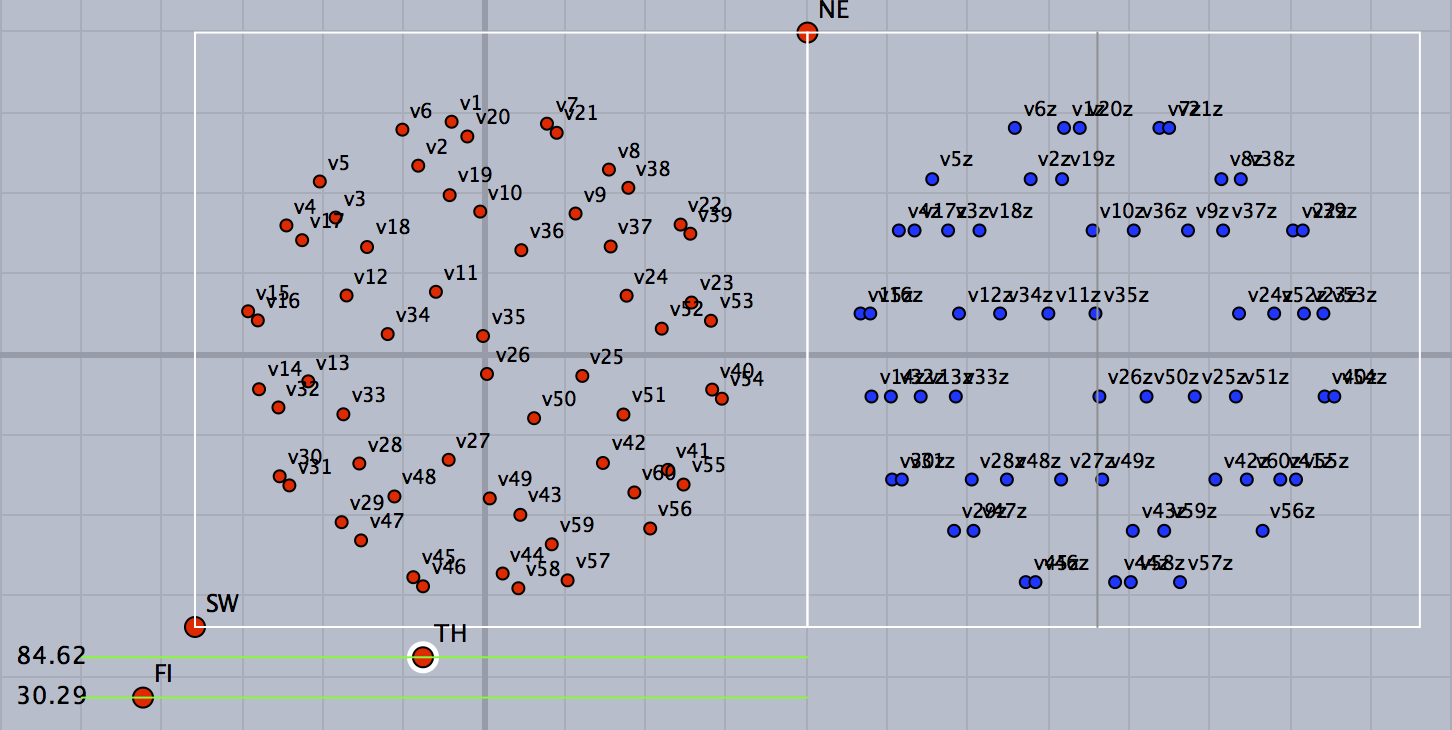
\includegraphics[bb=0 0 1452 730 , width=12cm]{Fig3d/phparadata01.png}\\
 \\
「Texview」「Exekc」ボタンを押すと陰線処理したデータがFhead.txt に書き出され,これを用いてFhead.texが作成される。そのため,Exekcボタンを押してから処理が完了するまでにかなり時間がかかる。(下図左)\\
 なお,もう一度実行すると,こんどは,Fhead.txt ができているために,これを読み込んでCinderellaの画面でも陰線処理された図が描かれる。\\
 全体の線種と,陰線の線種を\\
  \verb|Phparadata("1","s05",["dr,2","Hidden=do"]);|\\
で指定したのが下図右である。\\

  %%% /Users/Hannya/ketcindy/ketwork/template.tex 2016-8-11 22:26
%%% template.sce 2016-8-11 22:26
{\unitlength=6mm%
\begin{picture}%
(   7.60000,   7.37000)(  -3.60000,  -3.37000)%
\special{pn 8}%
%
\special{pa -98 -684}\special{pa -242 -660}%
\special{fp}%
\special{pa -242 -660}\special{pa -52 -640}%
\special{fp}%
\special{pa -52 -640}\special{pa 210 -651}%
\special{fp}%
\special{pa 210 -651}\special{pa 182 -678}%
\special{fp}%
\special{pa 182 -678}\special{pa -98 -684}%
\special{fp}%
\special{pa 182 -678}\special{pa 363 -543}%
\special{fp}%
\special{pa -582 -380}\special{pa -484 -508}%
\special{fp}%
\special{pa -484 -508}\special{pa -242 -660}%
\special{fp}%
\special{pa -662 100}\special{pa -694 -128}%
\special{fp}%
\special{pa -694 -128}\special{pa -582 -380}%
\special{fp}%
\special{pa -694 -128}\special{pa -666 -101}%
\special{fp}%
\special{pa -666 -101}\special{pa -536 -336}%
\special{fp}%
\special{pa -536 -336}\special{pa -484 -508}%
\special{fp}%
\special{pa -536 -336}\special{pa -346 -316}%
\special{fp}%
\special{pa -346 -316}\special{pa -104 -468}%
\special{fp}%
\special{pa -104 -468}\special{pa -52 -640}%
\special{fp}%
\special{pa 210 -651}\special{pa 420 -490}%
\special{fp}%
\special{pa 420 -490}\special{pa 602 -355}%
\special{fp}%
\special{pa 602 -355}\special{pa 573 -382}%
\special{fp}%
\special{pa 573 -382}\special{pa 363 -543}%
\special{fp}%
\special{pa -602 355}\special{pa -662 100}%
\special{fp}%
\special{pa -602 355}\special{pa -573 382}%
\special{fp}%
\special{pa -573 382}\special{pa -605 154}%
\special{fp}%
\special{pa -605 154}\special{pa -666 -101}%
\special{fp}%
\special{pa -605 154}\special{pa -415 174}%
\special{fp}%
\special{pa -415 174}\special{pa -285 -61}%
\special{fp}%
\special{pa -285 -61}\special{pa -346 -316}%
\special{fp}%
\special{pa -285 -61}\special{pa -6 -56}%
\special{fp}%
\special{pa -6 -56}\special{pa 106 -307}%
\special{fp}%
\special{pa 106 -307}\special{pa -104 -468}%
\special{fp}%
\special{pa 106 -307}\special{pa 368 -318}%
\special{fp}%
\special{pa 368 -318}\special{pa 420 -490}%
\special{fp}%
\special{pa 602 -355}\special{pa 662 -100}%
\special{fp}%
\special{pa 662 -100}\special{pa 694 128}%
\special{fp}%
\special{pa -182 678}\special{pa -363 543}%
\special{fp}%
\special{pa -363 543}\special{pa -573 382}%
\special{fp}%
\special{pa -363 543}\special{pa -265 415}%
\special{fp}%
\special{pa -265 415}\special{pa -415 174}%
\special{fp}%
\special{pa -265 415}\special{pa 14 420}%
\special{fp}%
\special{pa 14 420}\special{pa 144 185}%
\special{fp}%
\special{pa 144 185}\special{pa -6 -56}%
\special{fp}%
\special{pa 144 185}\special{pa 406 174}%
\special{fp}%
\special{pa 406 174}\special{pa 518 -77}%
\special{fp}%
\special{pa 518 -77}\special{pa 368 -318}%
\special{fp}%
\special{pa 518 -77}\special{pa 662 -100}%
\special{fp}%
\special{pa 694 128}\special{pa 582 380}%
\special{fp}%
\special{pa 582 380}\special{pa 484 508}%
\special{fp}%
\special{pa 484 508}\special{pa 242 660}%
\special{fp}%
\special{pa 242 660}\special{pa 98 684}%
\special{fp}%
\special{pa 98 684}\special{pa -182 678}%
\special{fp}%
\special{pa 98 684}\special{pa 196 555}%
\special{fp}%
\special{pa 196 555}\special{pa 14 420}%
\special{fp}%
\special{pa 196 555}\special{pa 438 403}%
\special{fp}%
\special{pa 438 403}\special{pa 406 174}%
\special{fp}%
\special{pa 438 403}\special{pa 582 380}%
\special{fp}%
\end{picture}}%    %%% /Users/Hannya/ketcindy/ketwork/template.tex 2016-8-11 22:33
%%% template.sce 2016-8-11 22:33
{\unitlength=6mm%
\begin{picture}%
(   7.60000,   7.37000)(  -3.60000,  -3.37000)%
\special{pn 8}%
%
\special{pn 16}%
\special{pa -98 -684}\special{pa -242 -660}%
\special{fp}%
\special{pa -242 -660}\special{pa -52 -640}%
\special{fp}%
\special{pa -52 -640}\special{pa 210 -651}%
\special{fp}%
\special{pa 210 -651}\special{pa 182 -678}%
\special{fp}%
\special{pa 182 -678}\special{pa -98 -684}%
\special{fp}%
\special{pa 182 -678}\special{pa 363 -543}%
\special{fp}%
\special{pa -582 -380}\special{pa -484 -508}%
\special{fp}%
\special{pa -484 -508}\special{pa -242 -660}%
\special{fp}%
\special{pa -662 100}\special{pa -694 -128}%
\special{fp}%
\special{pa -694 -128}\special{pa -582 -380}%
\special{fp}%
\special{pa -694 -128}\special{pa -666 -101}%
\special{fp}%
\special{pa -666 -101}\special{pa -536 -336}%
\special{fp}%
\special{pa -536 -336}\special{pa -484 -508}%
\special{fp}%
\special{pa -536 -336}\special{pa -346 -316}%
\special{fp}%
\special{pa -346 -316}\special{pa -104 -468}%
\special{fp}%
\special{pa -104 -468}\special{pa -52 -640}%
\special{fp}%
\special{pa 210 -651}\special{pa 420 -490}%
\special{fp}%
\special{pa 420 -490}\special{pa 602 -355}%
\special{fp}%
\special{pa 602 -355}\special{pa 573 -382}%
\special{fp}%
\special{pa 573 -382}\special{pa 363 -543}%
\special{fp}%
\special{pa -602 355}\special{pa -662 100}%
\special{fp}%
\special{pa -602 355}\special{pa -573 382}%
\special{fp}%
\special{pa -573 382}\special{pa -605 154}%
\special{fp}%
\special{pa -605 154}\special{pa -666 -101}%
\special{fp}%
\special{pa -605 154}\special{pa -415 174}%
\special{fp}%
\special{pa -415 174}\special{pa -285 -61}%
\special{fp}%
\special{pa -285 -61}\special{pa -346 -316}%
\special{fp}%
\special{pa -285 -61}\special{pa -6 -56}%
\special{fp}%
\special{pa -6 -56}\special{pa 106 -307}%
\special{fp}%
\special{pa 106 -307}\special{pa -104 -468}%
\special{fp}%
\special{pa 106 -307}\special{pa 368 -318}%
\special{fp}%
\special{pa 368 -318}\special{pa 420 -490}%
\special{fp}%
\special{pa 602 -355}\special{pa 662 -100}%
\special{fp}%
\special{pa 662 -100}\special{pa 694 128}%
\special{fp}%
\special{pa -182 678}\special{pa -363 543}%
\special{fp}%
\special{pa -363 543}\special{pa -573 382}%
\special{fp}%
\special{pa -363 543}\special{pa -265 415}%
\special{fp}%
\special{pa -265 415}\special{pa -415 174}%
\special{fp}%
\special{pa -265 415}\special{pa 14 420}%
\special{fp}%
\special{pa 14 420}\special{pa 144 185}%
\special{fp}%
\special{pa 144 185}\special{pa -6 -56}%
\special{fp}%
\special{pa 144 185}\special{pa 406 174}%
\special{fp}%
\special{pa 406 174}\special{pa 518 -77}%
\special{fp}%
\special{pa 518 -77}\special{pa 368 -318}%
\special{fp}%
\special{pa 518 -77}\special{pa 662 -100}%
\special{fp}%
\special{pa 694 128}\special{pa 582 380}%
\special{fp}%
\special{pa 582 380}\special{pa 484 508}%
\special{fp}%
\special{pa 484 508}\special{pa 242 660}%
\special{fp}%
\special{pa 242 660}\special{pa 98 684}%
\special{fp}%
\special{pa 98 684}\special{pa -182 678}%
\special{fp}%
\special{pa 98 684}\special{pa 196 555}%
\special{fp}%
\special{pa 196 555}\special{pa 14 420}%
\special{fp}%
\special{pa 196 555}\special{pa 438 403}%
\special{fp}%
\special{pa 438 403}\special{pa 406 174}%
\special{fp}%
\special{pa 438 403}\special{pa 582 380}%
\special{fp}%
\special{pn 8}%
\special{pn 8}%
\special{pa -95 -687}\special{pa -100 -680}\special{fp}\special{pa -120 -655}\special{pa -125 -648}\special{fp}%
\special{pa -144 -622}\special{pa -149 -616}\special{fp}\special{pa -169 -590}\special{pa -174 -584}\special{fp}%
\special{pa -193 -558}\special{pa -198 -552}\special{fp}\special{pn 8}%
\special{pa -192 -557}\special{pa -199 -553}\special{fp}\special{pa -227 -535}\special{pa -234 -531}\special{fp}%
\special{pa -261 -513}\special{pa -268 -509}\special{fp}\special{pa -296 -492}\special{pa -303 -488}\special{fp}%
\special{pa -331 -470}\special{pa -337 -466}\special{fp}\special{pa -365 -448}\special{pa -372 -444}\special{fp}%
\special{pa -400 -427}\special{pa -407 -422}\special{fp}\special{pa -434 -405}\special{pa -441 -401}\special{fp}%
\special{pn 8}%
\special{pa -586 -379}\special{pa -578 -380}\special{fp}\special{pa -550 -385}\special{pa -542 -386}\special{fp}%
\special{pa -514 -391}\special{pa -506 -392}\special{fp}\special{pa -478 -396}\special{pa -470 -398}\special{fp}%
\special{pa -442 -402}\special{pa -434 -403}\special{fp}\special{pn 8}%
\special{pa -438 -407}\special{pa -437 -399}\special{fp}\special{pa -433 -369}\special{pa -432 -361}\special{fp}%
\special{pa -428 -331}\special{pa -426 -323}\special{fp}\special{pa -422 -293}\special{pa -421 -285}\special{fp}%
\special{pa -417 -254}\special{pa -416 -247}\special{fp}\special{pa -412 -216}\special{pa -410 -209}\special{fp}%
\special{pa -406 -178}\special{pa -405 -170}\special{fp}\special{pn 8}%
\special{pa -404 -178}\special{pa -407 -171}\special{fp}\special{pa -420 -142}\special{pa -423 -135}\special{fp}%
\special{pa -436 -106}\special{pa -439 -99}\special{fp}\special{pa -452 -70}\special{pa -455 -63}\special{fp}%
\special{pa -468 -34}\special{pa -471 -27}\special{fp}\special{pa -484 2}\special{pa -487 9}\special{fp}%
\special{pa -500 38}\special{pa -504 45}\special{fp}\special{pa -516 74}\special{pa -520 81}\special{fp}%
\special{pn 8}%
\special{pa -666 101}\special{pa -658 100}\special{fp}\special{pa -630 95}\special{pa -622 94}\special{fp}%
\special{pa -594 89}\special{pa -586 88}\special{fp}\special{pa -558 84}\special{pa -550 82}\special{fp}%
\special{pa -522 78}\special{pa -514 77}\special{fp}\special{pn 8}%
\special{pa -410 -174}\special{pa -402 -175}\special{fp}\special{pa -372 -176}\special{pa -364 -176}\special{fp}%
\special{pa -335 -177}\special{pa -327 -178}\special{fp}\special{pa -297 -179}\special{pa -289 -179}\special{fp}%
\special{pa -260 -180}\special{pa -252 -181}\special{fp}\special{pa -223 -182}\special{pa -215 -182}\special{fp}%
\special{pa -185 -183}\special{pa -177 -184}\special{fp}\special{pa -148 -185}\special{pa -140 -185}\special{fp}%
\special{pn 8}%
\special{pa 366 -547}\special{pa 361 -540}\special{fp}\special{pa 341 -514}\special{pa 336 -508}\special{fp}%
\special{pa 317 -482}\special{pa 312 -476}\special{fp}\special{pa 292 -450}\special{pa 287 -444}\special{fp}%
\special{pa 268 -418}\special{pa 263 -411}\special{fp}\special{pn 8}%
\special{pa 269 -414}\special{pa 261 -415}\special{fp}\special{pa 229 -415}\special{pa 221 -415}\special{fp}%
\special{pa 190 -416}\special{pa 182 -416}\special{fp}\special{pa 150 -417}\special{pa 142 -417}\special{fp}%
\special{pa 110 -418}\special{pa 102 -418}\special{fp}\special{pa 70 -419}\special{pa 62 -419}\special{fp}%
\special{pa 30 -419}\special{pa 22 -420}\special{fp}\special{pa -10 -420}\special{pa -18 -420}\special{fp}%
\special{pn 8}%
\special{pa -199 -557}\special{pa -192 -552}\special{fp}\special{pa -169 -535}\special{pa -162 -530}\special{fp}%
\special{pa -138 -512}\special{pa -132 -508}\special{fp}\special{pa -108 -490}\special{pa -102 -485}\special{fp}%
\special{pa -78 -467}\special{pa -71 -463}\special{fp}\special{pa -48 -445}\special{pa -41 -440}\special{fp}%
\special{pa -17 -423}\special{pa -11 -418}\special{fp}\special{pn 8}%
\special{pa -146 -182}\special{pa -142 -189}\special{fp}\special{pa -127 -215}\special{pa -123 -222}\special{fp}%
\special{pa -109 -249}\special{pa -105 -256}\special{fp}\special{pa -90 -282}\special{pa -86 -289}\special{fp}%
\special{pa -72 -316}\special{pa -68 -323}\special{fp}\special{pa -53 -350}\special{pa -49 -357}\special{fp}%
\special{pa -35 -383}\special{pa -31 -390}\special{fp}\special{pa -16 -417}\special{pa -12 -424}\special{fp}%
\special{pn 8}%
\special{pa -520 74}\special{pa -516 81}\special{fp}\special{pa -499 108}\special{pa -494 115}\special{fp}%
\special{pa -477 143}\special{pa -473 149}\special{fp}\special{pa -456 177}\special{pa -452 184}\special{fp}%
\special{pa -435 211}\special{pa -430 218}\special{fp}\special{pa -413 246}\special{pa -409 253}\special{fp}%
\special{pa -392 280}\special{pa -388 287}\special{fp}\special{pa -370 315}\special{pa -366 321}\special{fp}%
\special{pn 8}%
\special{pa -367 314}\special{pa -369 322}\special{fp}\special{pa -378 349}\special{pa -380 356}\special{fp}%
\special{pa -388 383}\special{pa -390 391}\special{fp}\special{pa -398 417}\special{pa -401 425}\special{fp}%
\special{pa -409 452}\special{pa -411 459}\special{fp}\special{pa -419 486}\special{pa -421 494}\special{fp}%
\special{pn 8}%
\special{pa -605 353}\special{pa -599 358}\special{fp}\special{pa -575 375}\special{pa -568 380}\special{fp}%
\special{pa -544 398}\special{pa -538 403}\special{fp}\special{pa -514 420}\special{pa -508 425}\special{fp}%
\special{pa -484 443}\special{pa -477 447}\special{fp}\special{pa -454 465}\special{pa -447 470}\special{fp}%
\special{pa -423 488}\special{pa -417 492}\special{fp}\special{pn 8}%
\special{pa -146 -189}\special{pa -142 -182}\special{fp}\special{pa -125 -154}\special{pa -120 -147}\special{fp}%
\special{pa -103 -120}\special{pa -99 -113}\special{fp}\special{pa -82 -85}\special{pa -78 -79}\special{fp}%
\special{pa -60 -51}\special{pa -56 -44}\special{fp}\special{pa -39 -17}\special{pa -35 -10}\special{fp}%
\special{pa -18 18}\special{pa -13 25}\special{fp}\special{pa 4 52}\special{pa 8 59}\special{fp}%
\special{pn 8}%
\special{pa 7 52}\special{pa 4 59}\special{fp}\special{pa -9 88}\special{pa -12 95}\special{fp}%
\special{pa -25 124}\special{pa -28 131}\special{fp}\special{pa -41 160}\special{pa -44 167}\special{fp}%
\special{pa -57 196}\special{pa -60 203}\special{fp}\special{pa -73 232}\special{pa -76 239}\special{fp}%
\special{pa -89 268}\special{pa -92 275}\special{fp}\special{pa -105 304}\special{pa -108 311}\special{fp}%
\special{pn 8}%
\special{pa -372 318}\special{pa -364 318}\special{fp}\special{pa -335 317}\special{pa -327 316}\special{fp}%
\special{pa -298 315}\special{pa -290 315}\special{fp}\special{pa -260 314}\special{pa -252 313}\special{fp}%
\special{pa -223 312}\special{pa -215 312}\special{fp}\special{pa -185 310}\special{pa -177 310}\special{fp}%
\special{pa -148 309}\special{pa -140 309}\special{fp}\special{pa -110 307}\special{pa -102 307}\special{fp}%
\special{pn 8}%
\special{pa 263 -418}\special{pa 268 -411}\special{fp}\special{pa 285 -384}\special{pa 289 -377}\special{fp}%
\special{pa 306 -349}\special{pa 310 -342}\special{fp}\special{pa 327 -315}\special{pa 332 -308}\special{fp}%
\special{pa 349 -280}\special{pa 353 -274}\special{fp}\special{pa 370 -246}\special{pa 374 -239}\special{fp}%
\special{pa 392 -212}\special{pa 396 -205}\special{fp}\special{pa 413 -177}\special{pa 417 -170}\special{fp}%
\special{pn 8}%
\special{pa 417 -177}\special{pa 413 -170}\special{fp}\special{pa 398 -144}\special{pa 395 -137}\special{fp}%
\special{pa 380 -110}\special{pa 376 -103}\special{fp}\special{pa 361 -77}\special{pa 357 -70}\special{fp}%
\special{pa 343 -43}\special{pa 339 -36}\special{fp}\special{pa 324 -9}\special{pa 320 -2}\special{fp}%
\special{pa 306 24}\special{pa 302 31}\special{fp}\special{pa 287 58}\special{pa 283 65}\special{fp}%
\special{pn 8}%
\special{pa 2 56}\special{pa 10 56}\special{fp}\special{pa 42 56}\special{pa 50 57}\special{fp}%
\special{pa 82 57}\special{pa 90 57}\special{fp}\special{pa 122 58}\special{pa 130 58}\special{fp}%
\special{pa 161 59}\special{pa 169 59}\special{fp}\special{pa 201 60}\special{pa 209 60}\special{fp}%
\special{pa 241 60}\special{pa 249 61}\special{fp}\special{pa 281 61}\special{pa 289 61}\special{fp}%
\special{pn 8}%
\special{pa 573 -386}\special{pa 574 -378}\special{fp}\special{pa 578 -348}\special{pa 579 -340}\special{fp}%
\special{pa 583 -310}\special{pa 585 -302}\special{fp}\special{pa 589 -272}\special{pa 590 -264}\special{fp}%
\special{pa 594 -234}\special{pa 595 -226}\special{fp}\special{pa 599 -196}\special{pa 601 -188}\special{fp}%
\special{pa 605 -158}\special{pa 606 -150}\special{fp}\special{pn 8}%
\special{pa 411 -174}\special{pa 419 -173}\special{fp}\special{pa 449 -170}\special{pa 457 -169}\special{fp}%
\special{pa 487 -166}\special{pa 495 -165}\special{fp}\special{pa 525 -162}\special{pa 533 -161}\special{fp}%
\special{pa 563 -158}\special{pa 571 -157}\special{fp}\special{pa 601 -154}\special{pa 609 -153}\special{fp}%
\special{pn 8}%
\special{pa 56 640}\special{pa 48 641}\special{fp}\special{pa 18 642}\special{pa 10 642}\special{fp}%
\special{pa -19 643}\special{pa -27 644}\special{fp}\special{pa -56 645}\special{pa -64 645}\special{fp}%
\special{pa -94 646}\special{pa -102 647}\special{fp}\special{pa -131 648}\special{pa -139 648}\special{fp}%
\special{pa -169 649}\special{pa -177 650}\special{fp}\special{pa -206 651}\special{pa -214 651}\special{fp}%
\special{pn 8}%
\special{pa -423 488}\special{pa -417 492}\special{fp}\special{pa -393 511}\special{pa -387 515}\special{fp}%
\special{pa -363 534}\special{pa -357 538}\special{fp}\special{pa -333 557}\special{pa -327 561}\special{fp}%
\special{pa -303 580}\special{pa -297 584}\special{fp}\special{pa -273 603}\special{pa -267 608}\special{fp}%
\special{pa -243 626}\special{pa -237 631}\special{fp}\special{pa -213 649}\special{pa -207 654}\special{fp}%
\special{pn 8}%
\special{pa -213 648}\special{pa -207 654}\special{fp}\special{pa -185 675}\special{pa -179 681}\special{fp}%
\special{pn 8}%
\special{pa 284 57}\special{pa 286 65}\special{fp}\special{pa 293 94}\special{pa 295 102}\special{fp}%
\special{pa 302 130}\special{pa 303 138}\special{fp}\special{pa 310 167}\special{pa 312 175}\special{fp}%
\special{pa 319 203}\special{pa 321 211}\special{fp}\special{pa 327 240}\special{pa 329 247}\special{fp}%
\special{pa 336 276}\special{pa 338 284}\special{fp}\special{pa 345 313}\special{pa 347 320}\special{fp}%
\special{pn 8}%
\special{pa 349 314}\special{pa 342 319}\special{fp}\special{pa 314 336}\special{pa 308 340}\special{fp}%
\special{pa 280 358}\special{pa 273 362}\special{fp}\special{pa 245 379}\special{pa 239 384}\special{fp}%
\special{pa 211 401}\special{pa 204 405}\special{fp}\special{pa 176 423}\special{pa 169 427}\special{fp}%
\special{pa 142 445}\special{pa 135 449}\special{fp}\special{pa 107 466}\special{pa 100 471}\special{fp}%
\special{pn 8}%
\special{pa -110 305}\special{pa -103 310}\special{fp}\special{pa -80 328}\special{pa -73 333}\special{fp}%
\special{pa -50 351}\special{pa -43 356}\special{fp}\special{pa -20 374}\special{pa -13 379}\special{fp}%
\special{pa 10 397}\special{pa 17 402}\special{fp}\special{pa 40 420}\special{pa 47 425}\special{fp}%
\special{pa 70 443}\special{pa 77 448}\special{fp}\special{pa 100 466}\special{pa 107 471}\special{fp}%
\special{pn 8}%
\special{pa 51 644}\special{pa 53 637}\special{fp}\special{pa 61 610}\special{pa 63 602}\special{fp}%
\special{pa 71 575}\special{pa 74 568}\special{fp}\special{pa 82 541}\special{pa 84 533}\special{fp}%
\special{pa 92 507}\special{pa 94 499}\special{fp}\special{pa 102 472}\special{pa 105 465}\special{fp}%
\special{pn 8}%
\special{pa 697 131}\special{pa 691 125}\special{fp}\special{pa 669 104}\special{pa 663 99}\special{fp}%
\special{pn 8}%
\special{pa 604 -158}\special{pa 606 -150}\special{fp}\special{pa 613 -121}\special{pa 615 -113}\special{fp}%
\special{pa 622 -85}\special{pa 623 -77}\special{fp}\special{pa 630 -48}\special{pa 632 -41}\special{fp}%
\special{pa 639 -12}\special{pa 641 -4}\special{fp}\special{pa 648 25}\special{pa 649 32}\special{fp}%
\special{pa 656 61}\special{pa 658 69}\special{fp}\special{pa 665 97}\special{pa 667 105}\special{fp}%
\special{pn 8}%
\special{pa 668 98}\special{pa 664 105}\special{fp}\special{pa 649 131}\special{pa 645 138}\special{fp}%
\special{pa 631 165}\special{pa 627 172}\special{fp}\special{pa 612 199}\special{pa 608 206}\special{fp}%
\special{pa 593 232}\special{pa 590 239}\special{fp}\special{pa 575 266}\special{pa 571 273}\special{fp}%
\special{pa 556 299}\special{pa 553 306}\special{fp}\special{pa 538 333}\special{pa 534 340}\special{fp}%
\special{pn 8}%
\special{pa 342 316}\special{pa 350 317}\special{fp}\special{pa 380 320}\special{pa 388 321}\special{fp}%
\special{pa 418 324}\special{pa 426 325}\special{fp}\special{pa 456 328}\special{pa 464 329}\special{fp}%
\special{pa 494 332}\special{pa 502 333}\special{fp}\special{pa 532 336}\special{pa 540 337}\special{fp}%
\special{pn 8}%
\special{pa 537 333}\special{pa 535 340}\special{fp}\special{pa 527 367}\special{pa 524 375}\special{fp}%
\special{pa 516 401}\special{pa 514 409}\special{fp}\special{pa 506 436}\special{pa 504 443}\special{fp}%
\special{pa 496 470}\special{pa 493 478}\special{fp}\special{pa 485 505}\special{pa 483 512}\special{fp}%
\special{pn 8}%
\special{pa 48 640}\special{pa 56 641}\special{fp}\special{pa 86 644}\special{pa 94 645}\special{fp}%
\special{pa 124 648}\special{pa 132 649}\special{fp}\special{pa 162 652}\special{pa 170 653}\special{fp}%
\special{pa 200 656}\special{pa 208 657}\special{fp}\special{pa 238 660}\special{pa 246 661}\special{fp}%
\special{pn 8}%
\end{picture}}%\\

【注意】\\
 polyhedrons obj のデータを使って,続けて異なる多面体を描きたい場合は注意が必要である。Readobj()だけを変更して別のデータを読めばよさそうであるが,VertexEdgeFace() のname も(したがって,Phparadata()の第2引数も)書き換えないと,前のデータが残っていてうまくいかない。たとえば,上のコードで切頂十二面体を描いた後,正八面体(r02)を描こうとするならば,
\begin{verbatim}
 Setdirectory( Dirhead+"/data/polyhedrons_obj");
 phd=Readobj("r02.obj",["size=3"]);
 Setdirectory(Dirwork);
 VertexEdgeFace("2",phd,["Edg=nogeo"]);
 Phparadata("1","2");
\end{verbatim}
 のようにする。\\

\begin{flushright} \hyperlink{functionlist3d}{$\Rightarrow$関数一覧}\end{flushright}

\hypertarget{projcoordpara}{}
\item[関数] Projcoordpara(座標)
\item[機能] 投影座標を求める
\item[説明] 空間座標を投影した座標を求める。\\
 戻り値の第1,第2要素はCinderellaの描画面のx,y座標。第3要素はxy平面に垂直なzの座標で.投影面からの(符号付)距離を表す。\\
 \\
【例】\verb|Projcoordpara([3,1,2]);|\\
  戻り値は [-0.65,1.7,3.27]  となる。\\


\hypertarget{putaxes3d}{}
\item[関数] Putaxes3d([x,y,z])
\item[機能] 軸上に幾何点を作る。
\item[説明] 引数のリスト [x,y,z] に対し,点X(x,0,0) ,Y(0,y,0) , Z(0,0,z) および 原点Oを主画面上にとり,副画面上に対応する点Xz,Yz,Zz,Oz を作る。すでに同じ名称の点がある場合は,指定された位置に移動する。\\
 引数は,実数にすることもでき,Putaxes3d(a) は,Putaxes3d([a,a,a]) と同じになる。\\
【例】Putaxes3d(5); 原点と,$x(5,0,0),y(0,5,0),z(0,0,5)$ を作る。\\
  Putaxes3d([1,2,3]); 原点と,$x(1,0,0),y(0,2,0),z(0,0,3)$ を作る。\\

\begin{flushright} \hyperlink{functionlist3d}{$\Rightarrow$関数一覧}\end{flushright}

\hypertarget{putonCurve3d}{}
\item[関数] PutonCurve3d(点名,PD)
\item[機能] 空間曲線上に点をとる
\item[説明] プロットデータPDの曲線上に,点名の点をとる。\\
 とった点は固定点ではなく,曲線上にインシデントとなる。したがって,ドラッグして曲線上を動かすことができる。例は \hyperlink{partcrv3d}{Partcrv3d()} を参照のこと。\\
 \\

\hypertarget{putonseg3d}{}
\item[関数] Putonseg3d(点名,点1,点2)
\item[機能] 線分上に点を取る
\item[説明] 点1と点2の中点に,指定された名前の点を取る。点1と点2が線分として結ばれていなくてもよい。とった点は線分にインシデントとなる(線分が描かれていなくても)。点1と点2はリストにすることもできる。\\
 \\
【例】AとBの中点に点Cをとる。つぎのいずれでもよい。\\
  \verb|Putonseg3d("C",A,B);|\\
  \verb|Putonseg3d("C",[A,B]);|\\
 \\

\hypertarget{putpoint3d}{}
\item[関数] Putpoint3d(リスト,option)
\item[機能] 空間に幾何点を作図する
\item[説明] 点の名称と座標を与えて点を作図する。複数の点を一度に作図できる。\\
 optionは,"fix" または "free" (デフォルト)。\\
 "fix" をつけると,固定点(ドラッグで移動できない点)とする。同じ名称の点がすでに存在する場合は,指定した位置に移動して固定点とする。\\
 "free" をつけると,自由点(ドラッグで移動できる)とする。同じ名称の点がすでに存在する場合はなにもしない。\\
 \\
【例】いくつか記述例を示す。\\
  \verb|Putpoint3d(["A",[2,1,3]]);|\\
  \verb|Putpoint3d(["A",[1,1,1],"C",[1,0,1]],"fix");|\\
  \verb|Putpoint3d(["A",[2,1,3]],"free");|\\
 \\
 なお,この関数は幾何点を作るものであり,TeXには出力されない。TeXに点を出力するには,\hyperlink{pointdata}{Pointdata()} または \hyperlink{drwpt}{Drawpoint()}を併用する。\\
 空間における点の座標は,点名に"3d"を付加した名前の変数に代入される。たとえば,点Aの座標はA3dである。これにより,点の座標を取得できる。

\begin{flushright} \hyperlink{functionlist3d}{$\Rightarrow$関数一覧}\end{flushright}

\hypertarget{readobj}{}
\item[関数] Readobj(ファイル名)
\item[機能] objファイルを読み込む.
\item[説明] 小林・鈴木・三谷による多面体データ polyhedrons\_obj  を読み込む。\\
オプションは ["size=n"]  で,n倍したデータにする。負の数にすると上下が反転される。\\
データはKeTCindyのdataフォルダの中にある。したがって,次のようなスクリプトを書く。読み込むのは一度だけなので, Draw スロットではなくInitialization スロットに置けばよいが,コードの可読性を高めるには Draw スロットでもよい。
\begin{verbatim}
 Setdirectory( Dirhead+"/data/polyhedrons_obj");
 polydt=Readobj("r02.obj");
 Setdirectory(Dirwork);
\end{verbatim}
これで,r02.obj データが,変数 polydt に代入される。\\
この多面体データは,頂点リストと面リストからなっているが,頂点リストは座標のリストなので,読み込んで表示するときには,点の名称を v1,v2,・・・ とする。\\
読み込んだあとの使い方を含めて例を示す。\\

【例】正八面体を描く
\begin{verbatim}
 Setdirectory( Dirhead+"/data/polyhedrons_obj");
 polydt=Readobj("r02.obj",["size=2"]);
 Setdirectory(Dirwork);
 VertexEdgeFace("1",polydt,["Edg=nogeo"]);
 Nohiddenbyfaces("1","phf3d1");
\end{verbatim}
   %%% /Users/Hannya/ketcindy/ketwork/template.tex 2016-8-9 20:2
%%% template.sce 2016-8-9 20:2
{\unitlength=8mm%
\begin{picture}%
(   6.00000,   5.00000)(  -3.00000,  -2.00000)%
\special{pn 8}%
%
\special{pn 8}%
\special{pa -59 -253}\special{pa -51 -251}\special{fp}\special{pa -21 -240}\special{pa -13 -238}\special{fp}%
\special{pa 17 -228}\special{pa 25 -225}\special{fp}\special{pa 55 -215}\special{pa 62 -212}\special{fp}%
\special{pa 93 -202}\special{pa 100 -200}\special{fp}\special{pa 130 -189}\special{pa 138 -187}\special{fp}%
\special{pa 168 -177}\special{pa 176 -174}\special{fp}\special{pa 206 -164}\special{pa 214 -161}\special{fp}%
\special{pa 244 -151}\special{pa 251 -148}\special{fp}\special{pa 282 -138}\special{pa 289 -136}\special{fp}%
\special{pa 319 -125}\special{pa 327 -123}\special{fp}\special{pa 357 -113}\special{pa 365 -110}\special{fp}%
\special{pa 395 -100}\special{pa 403 -97}\special{fp}\special{pa 433 -87}\special{pa 440 -85}\special{fp}%
\special{pa 471 -74}\special{pa 478 -72}\special{fp}\special{pa 508 -62}\special{pa 516 -59}\special{fp}%
\special{pa 546 -49}\special{pa 554 -46}\special{fp}\special{pa 584 -36}\special{pa 592 -34}\special{fp}%
\special{pa 622 -23}\special{pa 629 -21}\special{fp}\special{pn 8}%
\special{pa 626 -22}\special{pa 0 577}%
\special{fp}%
\special{pn 8}%
\special{pa -55 -256}\special{pa -54 -248}\special{fp}\special{pa -52 -216}\special{pa -52 -208}\special{fp}%
\special{pa -50 -177}\special{pa -49 -169}\special{fp}\special{pa -47 -138}\special{pa -47 -130}\special{fp}%
\special{pa -45 -98}\special{pa -44 -90}\special{fp}\special{pa -42 -59}\special{pa -41 -51}\special{fp}%
\special{pa -39 -19}\special{pa -39 -11}\special{fp}\special{pa -37 20}\special{pa -36 28}\special{fp}%
\special{pa -34 60}\special{pa -34 68}\special{fp}\special{pa -32 99}\special{pa -31 107}\special{fp}%
\special{pa -29 139}\special{pa -28 147}\special{fp}\special{pa -26 178}\special{pa -26 186}\special{fp}%
\special{pa -24 218}\special{pa -23 226}\special{fp}\special{pa -21 257}\special{pa -21 265}\special{fp}%
\special{pa -19 296}\special{pa -18 304}\special{fp}\special{pa -16 336}\special{pa -15 344}\special{fp}%
\special{pa -13 375}\special{pa -13 383}\special{fp}\special{pa -11 415}\special{pa -10 423}\special{fp}%
\special{pa -8 454}\special{pa -8 462}\special{fp}\special{pa -5 494}\special{pa -5 502}\special{fp}%
\special{pa -3 533}\special{pa -2 541}\special{fp}\special{pa 0 573}\special{pa 0 581}\special{fp}%
\special{pn 8}%
\special{pa -626 22}\special{pa 0 577}%
\special{fp}%
\special{pn 8}%
\special{pa -51 -254}\special{pa -58 -250}\special{fp}\special{pa -87 -237}\special{pa -94 -233}\special{fp}%
\special{pa -122 -219}\special{pa -130 -216}\special{fp}\special{pa -158 -202}\special{pa -165 -199}\special{fp}%
\special{pa -194 -185}\special{pa -201 -182}\special{fp}\special{pa -230 -168}\special{pa -237 -165}\special{fp}%
\special{pa -265 -151}\special{pa -272 -147}\special{fp}\special{pa -301 -134}\special{pa -308 -130}\special{fp}%
\special{pa -337 -117}\special{pa -344 -113}\special{fp}\special{pa -372 -100}\special{pa -379 -96}\special{fp}%
\special{pa -408 -82}\special{pa -415 -79}\special{fp}\special{pa -444 -65}\special{pa -451 -62}\special{fp}%
\special{pa -479 -48}\special{pa -487 -45}\special{fp}\special{pa -515 -31}\special{pa -522 -28}\special{fp}%
\special{pa -551 -14}\special{pa -558 -10}\special{fp}\special{pa -586 3}\special{pa -594 7}\special{fp}%
\special{pa -622 20}\special{pa -629 24}\special{fp}\special{pn 8}%
\special{pa -626 22}\special{pa 0 -577}%
\special{fp}%
\special{pn 8}%
\special{pa -55 -248}\special{pa -54 -256}\special{fp}\special{pa -49 -289}\special{pa -47 -296}\special{fp}%
\special{pa -42 -329}\special{pa -40 -337}\special{fp}\special{pa -35 -370}\special{pa -34 -378}\special{fp}%
\special{pa -28 -410}\special{pa -27 -418}\special{fp}\special{pa -21 -451}\special{pa -20 -459}\special{fp}%
\special{pa -14 -491}\special{pa -13 -499}\special{fp}\special{pa -8 -532}\special{pa -6 -540}\special{fp}%
\special{pa -1 -573}\special{pa 1 -581}\special{fp}\special{pn 8}%
\special{pa 626 -22}\special{pa 0 -577}%
\special{fp}%
\special{pa 626 -22}\special{pa 55 252}%
\special{fp}%
\special{pa 55 252}\special{pa 0 577}%
\special{fp}%
\special{pa 55 252}\special{pa 0 -577}%
\special{fp}%
\special{pa 55 252}\special{pa -626 22}%
\special{fp}%
\end{picture}}%

\begin{flushright} \hyperlink{functionlist3d}{$\Rightarrow$関数一覧}\end{flushright}

\hypertarget{reflectpoint3d}{}
\item[関数] Reflectpoint3d(座標,リスト)
\item[機能] 点の鏡映点を求める
\item[説明] 第2引数のタイプにより,点に関する鏡映,直線に関する鏡映,面に関する鏡映のそれぞれの点の座標を返す。\\
 \\
【例】点A,B,C,Dを空間にとり,点Aの鏡映点の座標を求める。\\
  点Bに関する鏡映点   \verb|Reflectpoint3d(A3d,[B3d]);|\\
  直線BCに関する鏡映点 \verb|Reflectpoint3d(A3d,[B3d,C3d]);|\\
  平面BCDに関する鏡映点 \verb|Reflectpoint3d(A3d,[B3d,C3d,D3d]);|\\

\hypertarget{rotate3pt}{}
\item[関数] Rotate3pt(座標,vec,角度,中心点)
\item[機能] 点を回転する
\item[説明] 第1引数の座標の点を回転する。vecは回転軸の方向ベクトル。中心点は方向ベクトルの始点。第4引数を省略した場合は原点とする。\\
 \\
【例】点Aを(0,-1,0) に置いたときの記述例と結果(戻り値)\\
  \verb|Rotate3pt(A3d,[0,0,1],pi/2)|;     戻り値は [1,0,0]\\
  \verb|Rotate3pt(A3d,[0,0,1],pi/2,[1,1,1]);| 戻り値は[3,0,0]\\
 \\

\hypertarget{rotatedata3d}{}
\item[関数] Rotatedata3d(name,PDリスト,vec,角度,options)
\item[機能] プロットデータを回転
\item[説明] プロットデータを,原点を始点とするベクトルvec 周りに回転する。複数のプロットデータをまとめて回転することができる。\\
options として,中心点(vecの始点),線種を指定することができる。\\
 \\
【例】コード例と結果を示す。
\begin{verbatim}
 Xyzax3data("","x=[-5,4]","y=[-5,5]","z=[-5,4]",["a","O"]);
 Putpoint3d(["A",[0,-2,0],"B",[2,-2,0],"C",[1,-2,2],"D",[1,-2,3]],"fix");
 Spaceline("1",[A,B,C,A]);
 Spaceline([C,D]);
 Rotatedata3d("1",["sl3d1","CD3d"],[0,0,1],pi/2,["dr,2"]);
 Letter([A,"s","A",B,"w","B",C,"ne","C",D,"ne","D"]);
\end{verbatim}
これを\\
 \verb|Rotatedata3d("1",["sl3d1","CD3d"],[0,0,1],pi/2,[[1,0,0],"dr,2"]);|\\
とした場合が右図である。\\

 %%% /Users/Hannya/ketcindy/ketwork/template.tex 2016-8-15 20:33
%%% template.sce 2016-8-15 20:33
{\unitlength=8mm%
\begin{picture}%
(   7.77000,   5.78000)(  -4.42000,  -1.51000)%
\special{pn 8}%
%
\settowidth{\Width}{$x$}\setlength{\Width}{-0.5\Width}%
\settoheight{\Height}{$x$}\settodepth{\Depth}{$x$}\setlength{\Height}{-0.5\Height}\setlength{\Depth}{0.5\Depth}\addtolength{\Height}{\Depth}%
\put(-3.5455,-0.5866){\hspace*{\Width}\raisebox{\Height}{$x$}}%
%
%
\settowidth{\Width}{$y$}\setlength{\Width}{-0.5\Width}%
\settoheight{\Height}{$y$}\settodepth{\Depth}{$y$}\setlength{\Height}{-0.5\Height}\setlength{\Depth}{0.5\Depth}\addtolength{\Height}{\Depth}%
\put(2.8935,-1.1428){\hspace*{\Width}\raisebox{\Height}{$y$}}%
%
%
\settowidth{\Width}{$z$}\setlength{\Width}{-0.5\Width}%
\settoheight{\Height}{$z$}\settodepth{\Depth}{$z$}\setlength{\Height}{-0.5\Height}\setlength{\Depth}{0.5\Depth}\addtolength{\Height}{\Depth}%
\put(0.0000,4.0571){\hspace*{\Width}\raisebox{\Height}{$z$}}%
%
%
\special{pa 1055 -175}\special{pa -1058 175}%
\special{fp}%
\special{pa -856 -338}\special{pa 856 338}%
\special{fp}%
\special{pa 0 476}\special{pa 0 -1218}%
\special{fp}%
\special{pa -988 139}\special{pa -1058 175}\special{pa -980 187}\special{pa -984 163}%
\special{pa -988 139}\special{sh 1}\special{ip}%
\special{pn 1}%
\special{pa -988 139}\special{pa -1058 175}\special{pa -980 187}\special{pa -984 163}%
\special{pa -988 139}\special{pa -1058 175}%
\special{fp}%
\special{pn 8}%
\special{pa 777 333}\special{pa 856 338}\special{pa 795 288}\special{pa 786 310}\special{pa 777 333}%
\special{sh 1}\special{ip}%
\special{pn 1}%
\special{pa 777 333}\special{pa 856 338}\special{pa 795 288}\special{pa 786 310}\special{pa 777 333}%
\special{pa 856 338}%
\special{fp}%
\special{pn 8}%
\special{pa 24 -1143}\special{pa 0 -1218}\special{pa -24 -1143}\special{pa 0 -1143}%
\special{pa 24 -1143}\special{sh 1}\special{ip}%
\special{pn 1}%
\special{pa 24 -1143}\special{pa 0 -1218}\special{pa -24 -1143}\special{pa 0 -1143}%
\special{pa 24 -1143}\special{pa 0 -1218}%
\special{fp}%
\special{pn 8}%
\settowidth{\Width}{O}\setlength{\Width}{-1\Width}%
\settoheight{\Height}{O}\settodepth{\Depth}{O}\setlength{\Height}{-\Height}%
\put(-0.0500,-0.0500){\hspace*{\Width}\raisebox{\Height}{O}}%
%
%
\special{pa -342 -135}\special{pa -871 -48}\special{pa -607 -700}\special{pa -342 -135}%
\special{fp}%
\special{pa -607 -700}\special{pa -607 -1005}%
\special{fp}%
\special{pn 16}%
\special{pa -529 87}\special{pa -187 223}\special{pa -358 -454}\special{pa -529 87}%
\special{fp}%
\special{pa -358 -454}\special{pa -358 -758}%
\special{fp}%
\special{pn 8}%
\settowidth{\Width}{A}\setlength{\Width}{-0.5\Width}%
\settoheight{\Height}{A}\settodepth{\Depth}{A}\setlength{\Height}{-\Height}%
\put(-1.0867,0.3792){\hspace*{\Width}\raisebox{\Height}{A}}%
%
%
\settowidth{\Width}{B}\setlength{\Width}{-1\Width}%
\settoheight{\Height}{B}\settodepth{\Depth}{B}\setlength{\Height}{-0.5\Height}\setlength{\Depth}{0.5\Depth}\addtolength{\Height}{\Depth}%
\put(-2.8157,0.1514){\hspace*{\Width}\raisebox{\Height}{B}}%
%
%
\settowidth{\Width}{C}\setlength{\Width}{0\Width}%
\settoheight{\Height}{C}\settodepth{\Depth}{C}\setlength{\Height}{\Depth}%
\put(-1.8762,2.2739){\hspace*{\Width}\raisebox{\Height}{C}}%
%
%
\settowidth{\Width}{D}\setlength{\Width}{0\Width}%
\settoheight{\Height}{D}\settodepth{\Depth}{D}\setlength{\Height}{\Depth}%
\put(-1.8762,3.2406){\hspace*{\Width}\raisebox{\Height}{D}}%
%
%
\end{picture}}% %%% /Users/Hannya/ketcindy/ketwork/template.tex 2016-8-15 20:32
%%% template.sce 2016-8-15 20:32
{\unitlength=8mm%
\begin{picture}%
(   7.77000,   5.78000)(  -4.42000,  -1.51000)%
\special{pn 8}%
%
\settowidth{\Width}{$x$}\setlength{\Width}{-0.5\Width}%
\settoheight{\Height}{$x$}\settodepth{\Depth}{$x$}\setlength{\Height}{-0.5\Height}\setlength{\Depth}{0.5\Depth}\addtolength{\Height}{\Depth}%
\put(-3.5455,-0.5866){\hspace*{\Width}\raisebox{\Height}{$x$}}%
%
%
\settowidth{\Width}{$y$}\setlength{\Width}{-0.5\Width}%
\settoheight{\Height}{$y$}\settodepth{\Depth}{$y$}\setlength{\Height}{-0.5\Height}\setlength{\Depth}{0.5\Depth}\addtolength{\Height}{\Depth}%
\put(2.8935,-1.1428){\hspace*{\Width}\raisebox{\Height}{$y$}}%
%
%
\settowidth{\Width}{$z$}\setlength{\Width}{-0.5\Width}%
\settoheight{\Height}{$z$}\settodepth{\Depth}{$z$}\setlength{\Height}{-0.5\Height}\setlength{\Depth}{0.5\Depth}\addtolength{\Height}{\Depth}%
\put(0.0000,4.0571){\hspace*{\Width}\raisebox{\Height}{$z$}}%
%
%
\special{pa 1055 -175}\special{pa -1058 175}%
\special{fp}%
\special{pa -856 -338}\special{pa 856 338}%
\special{fp}%
\special{pa 0 476}\special{pa 0 -1218}%
\special{fp}%
\special{pa -988 139}\special{pa -1058 175}\special{pa -980 187}\special{pa -984 163}%
\special{pa -988 139}\special{sh 1}\special{ip}%
\special{pn 1}%
\special{pa -988 139}\special{pa -1058 175}\special{pa -980 187}\special{pa -984 163}%
\special{pa -988 139}\special{pa -1058 175}%
\special{fp}%
\special{pn 8}%
\special{pa 777 333}\special{pa 856 338}\special{pa 795 288}\special{pa 786 310}\special{pa 777 333}%
\special{sh 1}\special{ip}%
\special{pn 1}%
\special{pa 777 333}\special{pa 856 338}\special{pa 795 288}\special{pa 786 310}\special{pa 777 333}%
\special{pa 856 338}%
\special{fp}%
\special{pn 8}%
\special{pa 24 -1143}\special{pa 0 -1218}\special{pa -24 -1143}\special{pa 0 -1143}%
\special{pa 24 -1143}\special{sh 1}\special{ip}%
\special{pn 1}%
\special{pa 24 -1143}\special{pa 0 -1218}\special{pa -24 -1143}\special{pa 0 -1143}%
\special{pa 24 -1143}\special{pa 0 -1218}%
\special{fp}%
\special{pn 8}%
\settowidth{\Width}{O}\setlength{\Width}{-1\Width}%
\settoheight{\Height}{O}\settodepth{\Depth}{O}\setlength{\Height}{-\Height}%
\put(-0.0500,-0.0500){\hspace*{\Width}\raisebox{\Height}{O}}%
%
%
\special{pa -342 -135}\special{pa -871 -48}\special{pa -607 -700}\special{pa -342 -135}%
\special{fp}%
\special{pa -607 -700}\special{pa -607 -1005}%
\special{fp}%
\special{pn 16}%
\special{pa -964 64}\special{pa -622 199}\special{pa -793 -478}\special{pa -964 64}%
\special{fp}%
\special{pa -793 -478}\special{pa -793 -782}%
\special{fp}%
\special{pn 8}%
\settowidth{\Width}{A}\setlength{\Width}{-0.5\Width}%
\settoheight{\Height}{A}\settodepth{\Depth}{A}\setlength{\Height}{-\Height}%
\put(-1.0867,0.3792){\hspace*{\Width}\raisebox{\Height}{A}}%
%
%
\settowidth{\Width}{B}\setlength{\Width}{-1\Width}%
\settoheight{\Height}{B}\settodepth{\Depth}{B}\setlength{\Height}{-0.5\Height}\setlength{\Depth}{0.5\Depth}\addtolength{\Height}{\Depth}%
\put(-2.8157,0.1514){\hspace*{\Width}\raisebox{\Height}{B}}%
%
%
\settowidth{\Width}{C}\setlength{\Width}{0\Width}%
\settoheight{\Height}{C}\settodepth{\Depth}{C}\setlength{\Height}{\Depth}%
\put(-1.8762,2.2739){\hspace*{\Width}\raisebox{\Height}{C}}%
%
%
\settowidth{\Width}{D}\setlength{\Width}{0\Width}%
\settoheight{\Height}{D}\settodepth{\Depth}{D}\setlength{\Height}{\Depth}%
\put(-1.8762,3.2406){\hspace*{\Width}\raisebox{\Height}{D}}%
%
%
\end{picture}}%\\

\hypertarget{sf3data}{}
\item[関数] Sf3data(name,リスト,options)
\item[機能] 陰線処理なしの曲面をワイヤーフレームモデルで描く
\item[説明] リストは,関数式と定義域,境界指定をそれぞれ文字列にしたもののリスト。\\
optionsは,解像度(各変数に対応する分割数)とメッシュの密度(縦横)。\\
解像度は,"Num=[a,b]" で指定。初期値はa,bとも25\\
メッシュ密度は,"Wire=[a,b]" で指定。初期値はa,bとも20\\
境界の指定は"ewsn"で行う。\\
関数式のパターンはつぎの3通り。\\
 \\
(1) $z=f(x,y)$\\
 【例】:$z=x^2-y^2$を定義域$x=[-2,2],y=[-2,2]$ で描画する。\\
   \verb|Sf3data("1",["z=x^2-y^2","x=[-2,2]","y=[-2,2]"])|;\\
       %%% /Users/Hannya/ketcindy/ketwork/template.tex 2016-8-7 16:45
%%% template.sce 2016-8-7 16:45
{\unitlength=4mm%
\begin{picture}%
(  10.00000,  10.00000)(  -5.00000,  -5.00000)%
\special{pn 8}%
%
\settowidth{\Width}{$x$}\setlength{\Width}{-0.5\Width}%
\settoheight{\Height}{$x$}\settodepth{\Depth}{$x$}\setlength{\Height}{-0.5\Height}\setlength{\Depth}{0.5\Depth}\addtolength{\Height}{\Depth}%
\put(-4.6011,-1.1540){\hspace*{\Width}\raisebox{\Height}{$x$}}%
%
%
\settowidth{\Width}{$y$}\setlength{\Width}{-0.5\Width}%
\settoheight{\Height}{$y$}\settodepth{\Depth}{$y$}\setlength{\Height}{-0.5\Height}\setlength{\Depth}{0.5\Depth}\addtolength{\Height}{\Depth}%
\put(2.4854,-2.2142){\hspace*{\Width}\raisebox{\Height}{$y$}}%
%
%
\settowidth{\Width}{$z$}\setlength{\Width}{-0.5\Width}%
\settoheight{\Height}{$z$}\settodepth{\Depth}{$z$}\setlength{\Height}{-0.5\Height}\setlength{\Depth}{0.5\Depth}\addtolength{\Height}{\Depth}%
\put(0.0000,4.5961){\hspace*{\Width}\raisebox{\Height}{$z$}}%
%
%
\special{pa 696 -174}\special{pa -696 174}%
\special{fp}%
\special{pa -369 -329}\special{pa 369 329}%
\special{fp}%
\special{pa 0 694}\special{pa 0 -694}%
\special{fp}%
\special{pa 131 -201}\special{pa 107 -107}\special{pa 84 -20}\special{pa 61 59}\special{pa 38 130}%
\special{pa 15 194}\special{pa -9 250}\special{pa -32 298}\special{pa -55 339}\special{pa -78 371}%
\special{pa -101 397}\special{pa -124 414}\special{pa -148 424}\special{pa -171 426}%
\special{pa -194 420}\special{pa -217 406}\special{pa -240 385}\special{pa -264 356}%
\special{pa -287 320}\special{pa -310 275}\special{pa -333 223}\special{pa -356 164}%
\special{pa -379 96}\special{pa -403 21}\special{pa -426 -62}%
\special{fp}%
\special{pa 145 -294}\special{pa 122 -199}\special{pa 99 -112}\special{pa 76 -33}%
\special{pa 53 38}\special{pa 29 102}\special{pa 6 158}\special{pa -17 206}\special{pa -40 246}%
\special{pa -63 279}\special{pa -86 304}\special{pa -110 322}\special{pa -133 331}%
\special{pa -156 333}\special{pa -179 327}\special{pa -202 314}\special{pa -226 293}%
\special{pa -249 264}\special{pa -272 227}\special{pa -295 183}\special{pa -318 131}%
\special{pa -342 71}\special{pa -365 4}\special{pa -388 -71}\special{pa -411 -154}%
\special{fp}%
\special{pa 160 -375}\special{pa 137 -280}\special{pa 114 -194}\special{pa 91 -115}%
\special{pa 67 -43}\special{pa 44 20}\special{pa 21 76}\special{pa -2 125}\special{pa -25 165}%
\special{pa -49 198}\special{pa -72 223}\special{pa -95 240}\special{pa -118 250}%
\special{pa -141 252}\special{pa -164 246}\special{pa -188 233}\special{pa -211 212}%
\special{pa -234 183}\special{pa -257 146}\special{pa -280 102}\special{pa -304 50}%
\special{pa -327 -10}\special{pa -350 -77}\special{pa -373 -152}\special{pa -396 -235}%
\special{fp}%
\special{pa 175 -445}\special{pa 152 -350}\special{pa 129 -264}\special{pa 105 -185}%
\special{pa 82 -113}\special{pa 59 -50}\special{pa 36 6}\special{pa 13 54}\special{pa -11 95}%
\special{pa -34 128}\special{pa -57 153}\special{pa -80 170}\special{pa -103 180}%
\special{pa -127 182}\special{pa -150 176}\special{pa -173 163}\special{pa -196 142}%
\special{pa -219 113}\special{pa -242 76}\special{pa -266 32}\special{pa -289 -20}%
\special{pa -312 -80}\special{pa -335 -147}\special{pa -358 -223}\special{pa -382 -305}%
\special{fp}%
\special{pa 190 -504}\special{pa 166 -409}\special{pa 143 -323}\special{pa 120 -244}%
\special{pa 97 -172}\special{pa 74 -109}\special{pa 51 -53}\special{pa 27 -5}\special{pa 4 36}%
\special{pa -19 69}\special{pa -42 94}\special{pa -65 111}\special{pa -89 121}\special{pa -112 123}%
\special{pa -135 117}\special{pa -158 104}\special{pa -181 83}\special{pa -205 54}%
\special{pa -228 17}\special{pa -251 -27}\special{pa -274 -79}\special{pa -297 -139}%
\special{pa -320 -206}\special{pa -344 -282}\special{pa -367 -364}%
\special{fp}%
\special{pa 204 -552}\special{pa 181 -457}\special{pa 158 -371}\special{pa 135 -292}%
\special{pa 112 -220}\special{pa 88 -157}\special{pa 65 -101}\special{pa 42 -52}\special{pa 19 -12}%
\special{pa -4 21}\special{pa -27 46}\special{pa -51 63}\special{pa -74 73}\special{pa -97 75}%
\special{pa -120 69}\special{pa -143 56}\special{pa -167 35}\special{pa -190 6}\special{pa -213 -31}%
\special{pa -236 -75}\special{pa -259 -127}\special{pa -282 -187}\special{pa -306 -254}%
\special{pa -329 -329}\special{pa -352 -412}%
\special{fp}%
\special{pa 219 -589}\special{pa 196 -494}\special{pa 173 -407}\special{pa 150 -328}%
\special{pa 126 -257}\special{pa 103 -193}\special{pa 80 -137}\special{pa 57 -89}%
\special{pa 34 -49}\special{pa 11 -16}\special{pa -13 9}\special{pa -36 27}\special{pa -59 36}%
\special{pa -82 38}\special{pa -105 32}\special{pa -129 19}\special{pa -152 -2}\special{pa -175 -31}%
\special{pa -198 -68}\special{pa -221 -112}\special{pa -245 -164}\special{pa -268 -224}%
\special{pa -291 -291}\special{pa -314 -366}\special{pa -337 -449}%
\special{fp}%
\special{pa 234 -614}\special{pa 211 -520}\special{pa 188 -433}\special{pa 164 -354}%
\special{pa 141 -283}\special{pa 118 -219}\special{pa 95 -163}\special{pa 72 -115}%
\special{pa 48 -74}\special{pa 25 -42}\special{pa 2 -17}\special{pa -21 1}\special{pa -44 11}%
\special{pa -67 12}\special{pa -91 7}\special{pa -114 -7}\special{pa -137 -28}\special{pa -160 -57}%
\special{pa -183 -93}\special{pa -207 -138}\special{pa -230 -190}\special{pa -253 -249}%
\special{pa -276 -317}\special{pa -299 -392}\special{pa -323 -475}%
\special{fp}%
\special{pa 249 -629}\special{pa 226 -535}\special{pa 202 -448}\special{pa 179 -369}%
\special{pa 156 -297}\special{pa 133 -234}\special{pa 110 -178}\special{pa 86 -130}%
\special{pa 63 -89}\special{pa 40 -56}\special{pa 17 -31}\special{pa -6 -14}\special{pa -30 -4}%
\special{pa -53 -2}\special{pa -76 -8}\special{pa -99 -21}\special{pa -122 -43}\special{pa -145 -71}%
\special{pa -169 -108}\special{pa -192 -152}\special{pa -215 -204}\special{pa -238 -264}%
\special{pa -261 -331}\special{pa -285 -407}\special{pa -308 -489}%
\special{fp}%
\special{pa 263 -632}\special{pa 240 -538}\special{pa 217 -451}\special{pa 194 -372}%
\special{pa 171 -301}\special{pa 148 -237}\special{pa 124 -181}\special{pa 101 -133}%
\special{pa 78 -93}\special{pa 55 -60}\special{pa 32 -35}\special{pa 8 -17}\special{pa -15 -8}%
\special{pa -38 -6}\special{pa -61 -11}\special{pa -84 -25}\special{pa -108 -46}\special{pa -131 -75}%
\special{pa -154 -111}\special{pa -177 -156}\special{pa -200 -208}\special{pa -223 -268}%
\special{pa -247 -335}\special{pa -270 -410}\special{pa -293 -493}%
\special{fp}%
\special{pa 278 -625}\special{pa 255 -530}\special{pa 232 -444}\special{pa 209 -365}%
\special{pa 185 -293}\special{pa 162 -230}\special{pa 139 -174}\special{pa 116 -125}%
\special{pa 93 -85}\special{pa 70 -52}\special{pa 46 -27}\special{pa 23 -10}\special{pa 0 0}%
\special{pa -23 2}\special{pa -46 -4}\special{pa -70 -17}\special{pa -93 -38}\special{pa -116 -67}%
\special{pa -139 -104}\special{pa -162 -148}\special{pa -185 -200}\special{pa -209 -260}%
\special{pa -232 -327}\special{pa -255 -402}\special{pa -278 -485}%
\special{fp}%
\special{pa 293 -606}\special{pa 270 -512}\special{pa 247 -425}\special{pa 223 -346}%
\special{pa 200 -275}\special{pa 177 -211}\special{pa 154 -155}\special{pa 131 -107}%
\special{pa 108 -66}\special{pa 84 -33}\special{pa 61 -8}\special{pa 38 9}\special{pa 15 19}%
\special{pa -8 21}\special{pa -32 15}\special{pa -55 1}\special{pa -78 -20}\special{pa -101 -49}%
\special{pa -124 -85}\special{pa -148 -129}\special{pa -171 -181}\special{pa -194 -241}%
\special{pa -217 -309}\special{pa -240 -384}\special{pa -263 -467}%
\special{fp}%
\special{pa 308 -576}\special{pa 285 -482}\special{pa 261 -395}\special{pa 238 -316}%
\special{pa 215 -245}\special{pa 192 -181}\special{pa 169 -125}\special{pa 145 -77}%
\special{pa 122 -36}\special{pa 99 -4}\special{pa 76 21}\special{pa 53 39}\special{pa 30 49}%
\special{pa 6 50}\special{pa -17 45}\special{pa -40 31}\special{pa -63 10}\special{pa -86 -19}%
\special{pa -110 -55}\special{pa -133 -100}\special{pa -156 -152}\special{pa -179 -211}%
\special{pa -202 -279}\special{pa -226 -354}\special{pa -249 -437}%
\special{fp}%
\special{pa 323 -535}\special{pa 299 -441}\special{pa 276 -354}\special{pa 253 -275}%
\special{pa 230 -204}\special{pa 207 -140}\special{pa 183 -84}\special{pa 160 -36}%
\special{pa 137 4}\special{pa 114 37}\special{pa 91 62}\special{pa 67 80}\special{pa 44 89}%
\special{pa 21 91}\special{pa -2 86}\special{pa -25 72}\special{pa -48 51}\special{pa -72 22}%
\special{pa -95 -14}\special{pa -118 -59}\special{pa -141 -111}\special{pa -164 -170}%
\special{pa -188 -238}\special{pa -211 -313}\special{pa -234 -396}%
\special{fp}%
\special{pa 337 -483}\special{pa 314 -389}\special{pa 291 -302}\special{pa 268 -223}%
\special{pa 245 -152}\special{pa 221 -88}\special{pa 198 -32}\special{pa 175 16}\special{pa 152 56}%
\special{pa 129 89}\special{pa 105 114}\special{pa 82 132}\special{pa 59 141}\special{pa 36 143}%
\special{pa 13 138}\special{pa -11 124}\special{pa -34 103}\special{pa -57 74}\special{pa -80 38}%
\special{pa -103 -7}\special{pa -126 -59}\special{pa -150 -118}\special{pa -173 -186}%
\special{pa -196 -261}\special{pa -219 -344}%
\special{fp}%
\special{pa 352 -420}\special{pa 329 -326}\special{pa 306 -239}\special{pa 282 -160}%
\special{pa 259 -89}\special{pa 236 -25}\special{pa 213 31}\special{pa 190 79}\special{pa 167 120}%
\special{pa 143 152}\special{pa 120 177}\special{pa 97 195}\special{pa 74 205}\special{pa 51 206}%
\special{pa 27 201}\special{pa 4 187}\special{pa -19 166}\special{pa -42 137}\special{pa -65 101}%
\special{pa -88 56}\special{pa -112 4}\special{pa -135 -55}\special{pa -158 -123}%
\special{pa -181 -198}\special{pa -204 -281}%
\special{fp}%
\special{pa 367 -346}\special{pa 344 -252}\special{pa 320 -165}\special{pa 297 -86}%
\special{pa 274 -14}\special{pa 251 49}\special{pa 228 105}\special{pa 205 153}\special{pa 181 194}%
\special{pa 158 227}\special{pa 135 252}\special{pa 112 269}\special{pa 89 279}\special{pa 65 281}%
\special{pa 42 275}\special{pa 19 261}\special{pa -4 240}\special{pa -27 211}\special{pa -51 175}%
\special{pa -74 131}\special{pa -97 79}\special{pa -120 19}\special{pa -143 -49}\special{pa -166 -124}%
\special{pa -190 -207}%
\special{fp}%
\special{pa 382 -261}\special{pa 358 -166}\special{pa 335 -80}\special{pa 312 -1}%
\special{pa 289 71}\special{pa 266 134}\special{pa 242 190}\special{pa 219 239}\special{pa 196 279}%
\special{pa 173 312}\special{pa 150 337}\special{pa 127 354}\special{pa 103 364}\special{pa 80 366}%
\special{pa 57 360}\special{pa 34 347}\special{pa 11 326}\special{pa -13 297}\special{pa -36 260}%
\special{pa -59 216}\special{pa -82 164}\special{pa -105 104}\special{pa -129 37}%
\special{pa -152 -38}\special{pa -175 -121}%
\special{fp}%
\special{pa 396 -164}\special{pa 373 -70}\special{pa 350 17}\special{pa 327 96}\special{pa 304 167}%
\special{pa 280 231}\special{pa 257 287}\special{pa 234 335}\special{pa 211 376}\special{pa 188 408}%
\special{pa 164 433}\special{pa 141 451}\special{pa 118 460}\special{pa 95 462}\special{pa 72 457}%
\special{pa 49 443}\special{pa 25 422}\special{pa 2 393}\special{pa -21 357}\special{pa -44 312}%
\special{pa -67 260}\special{pa -91 201}\special{pa -114 133}\special{pa -137 58}%
\special{pa -160 -25}%
\special{fp}%
\special{pa 411 -57}\special{pa 388 38}\special{pa 365 124}\special{pa 342 203}\special{pa 318 275}%
\special{pa 295 338}\special{pa 272 394}\special{pa 249 443}\special{pa 226 483}\special{pa 202 516}%
\special{pa 179 541}\special{pa 156 558}\special{pa 133 568}\special{pa 110 570}\special{pa 86 564}%
\special{pa 63 551}\special{pa 40 530}\special{pa 17 501}\special{pa -6 464}\special{pa -29 420}%
\special{pa -53 368}\special{pa -76 308}\special{pa -99 241}\special{pa -122 166}%
\special{pa -145 83}%
\special{fp}%
\special{pa 426 62}\special{pa 403 156}\special{pa 379 243}\special{pa 356 322}\special{pa 333 393}%
\special{pa 310 457}\special{pa 287 513}\special{pa 264 561}\special{pa 240 602}\special{pa 217 634}%
\special{pa 194 660}\special{pa 171 677}\special{pa 148 687}\special{pa 124 689}\special{pa 101 683}%
\special{pa 78 669}\special{pa 55 648}\special{pa 32 619}\special{pa 9 583}\special{pa -15 538}%
\special{pa -38 486}\special{pa -61 427}\special{pa -84 359}\special{pa -107 284}%
\special{pa -131 201}%
\special{fp}%
\special{pa 131 -201}\special{pa 143 -279}\special{pa 155 -349}\special{pa 168 -411}%
\special{pa 180 -466}\special{pa 192 -513}\special{pa 204 -552}\special{pa 217 -583}%
\special{pa 229 -607}\special{pa 241 -623}\special{pa 254 -631}\special{pa 266 -632}%
\special{pa 278 -625}\special{pa 291 -610}\special{pa 303 -588}\special{pa 315 -557}%
\special{pa 327 -519}\special{pa 340 -474}\special{pa 352 -420}\special{pa 364 -359}%
\special{pa 377 -290}\special{pa 389 -214}\special{pa 401 -130}\special{pa 414 -38}%
\special{pa 426 62}%
\special{fp}%
\special{pa 103 -89}\special{pa 115 -167}\special{pa 127 -237}\special{pa 140 -299}%
\special{pa 152 -353}\special{pa 164 -400}\special{pa 177 -439}\special{pa 189 -471}%
\special{pa 201 -495}\special{pa 213 -511}\special{pa 226 -519}\special{pa 238 -520}%
\special{pa 250 -512}\special{pa 263 -498}\special{pa 275 -475}\special{pa 287 -445}%
\special{pa 300 -407}\special{pa 312 -361}\special{pa 324 -308}\special{pa 337 -247}%
\special{pa 349 -178}\special{pa 361 -102}\special{pa 373 -17}\special{pa 386 75}%
\special{pa 398 174}%
\special{fp}%
\special{pa 75 12}\special{pa 87 -65}\special{pa 100 -135}\special{pa 112 -197}\special{pa 124 -252}%
\special{pa 136 -299}\special{pa 149 -338}\special{pa 161 -370}\special{pa 173 -393}%
\special{pa 186 -409}\special{pa 198 -418}\special{pa 210 -418}\special{pa 223 -411}%
\special{pa 235 -396}\special{pa 247 -374}\special{pa 259 -344}\special{pa 272 -306}%
\special{pa 284 -260}\special{pa 296 -207}\special{pa 309 -145}\special{pa 321 -77}%
\special{pa 333 0}\special{pa 346 84}\special{pa 358 176}\special{pa 370 276}%
\special{fp}%
\special{pa 47 103}\special{pa 59 25}\special{pa 72 -45}\special{pa 84 -107}\special{pa 96 -162}%
\special{pa 109 -209}\special{pa 121 -248}\special{pa 133 -279}\special{pa 146 -303}%
\special{pa 158 -319}\special{pa 170 -327}\special{pa 182 -328}\special{pa 195 -321}%
\special{pa 207 -306}\special{pa 219 -284}\special{pa 232 -253}\special{pa 244 -215}%
\special{pa 256 -170}\special{pa 269 -116}\special{pa 281 -55}\special{pa 293 14}%
\special{pa 305 90}\special{pa 318 174}\special{pa 330 266}\special{pa 342 366}%
\special{fp}%
\special{pa 19 182}\special{pa 32 104}\special{pa 44 34}\special{pa 56 -28}\special{pa 69 -83}%
\special{pa 81 -130}\special{pa 93 -169}\special{pa 105 -200}\special{pa 118 -224}%
\special{pa 130 -240}\special{pa 142 -248}\special{pa 155 -249}\special{pa 167 -242}%
\special{pa 179 -227}\special{pa 192 -204}\special{pa 204 -174}\special{pa 216 -136}%
\special{pa 228 -91}\special{pa 241 -37}\special{pa 253 24}\special{pa 265 93}\special{pa 278 169}%
\special{pa 290 253}\special{pa 302 345}\special{pa 315 445}%
\special{fp}%
\special{pa -9 250}\special{pa 4 172}\special{pa 16 102}\special{pa 28 40}\special{pa 41 -15}%
\special{pa 53 -61}\special{pa 65 -101}\special{pa 78 -132}\special{pa 90 -156}\special{pa 102 -172}%
\special{pa 115 -180}\special{pa 127 -181}\special{pa 139 -174}\special{pa 151 -159}%
\special{pa 164 -136}\special{pa 176 -106}\special{pa 188 -68}\special{pa 201 -22}%
\special{pa 213 31}\special{pa 225 92}\special{pa 238 161}\special{pa 250 237}\special{pa 262 321}%
\special{pa 274 413}\special{pa 287 513}%
\special{fp}%
\special{pa -36 307}\special{pa -24 229}\special{pa -12 159}\special{pa 1 97}\special{pa 13 42}%
\special{pa 25 -5}\special{pa 37 -44}\special{pa 50 -75}\special{pa 62 -99}\special{pa 74 -115}%
\special{pa 87 -123}\special{pa 99 -124}\special{pa 111 -117}\special{pa 124 -102}%
\special{pa 136 -79}\special{pa 148 -49}\special{pa 160 -11}\special{pa 173 34}\special{pa 185 88}%
\special{pa 197 149}\special{pa 210 218}\special{pa 222 294}\special{pa 234 378}\special{pa 247 470}%
\special{pa 259 570}%
\special{fp}%
\special{pa -64 353}\special{pa -52 275}\special{pa -40 205}\special{pa -27 143}\special{pa -15 88}%
\special{pa -3 41}\special{pa 10 2}\special{pa 22 -29}\special{pa 34 -53}\special{pa 47 -69}%
\special{pa 59 -77}\special{pa 71 -78}\special{pa 83 -71}\special{pa 96 -56}\special{pa 108 -34}%
\special{pa 120 -3}\special{pa 133 35}\special{pa 145 80}\special{pa 157 134}\special{pa 170 195}%
\special{pa 182 263}\special{pa 194 340}\special{pa 206 424}\special{pa 219 516}\special{pa 231 616}%
\special{fp}%
\special{pa -92 387}\special{pa -80 310}\special{pa -67 240}\special{pa -55 177}\special{pa -43 123}%
\special{pa -30 76}\special{pa -18 37}\special{pa -6 5}\special{pa 6 -18}\special{pa 19 -34}%
\special{pa 31 -43}\special{pa 43 -43}\special{pa 56 -36}\special{pa 68 -21}\special{pa 80 1}%
\special{pa 93 31}\special{pa 105 69}\special{pa 117 115}\special{pa 129 168}\special{pa 142 229}%
\special{pa 154 298}\special{pa 166 375}\special{pa 179 459}\special{pa 191 551}\special{pa 203 650}%
\special{fp}%
\special{pa -120 411}\special{pa -108 333}\special{pa -95 263}\special{pa -83 201}%
\special{pa -71 147}\special{pa -58 100}\special{pa -46 60}\special{pa -34 29}\special{pa -21 5}%
\special{pa -9 -11}\special{pa 3 -19}\special{pa 16 -20}\special{pa 28 -13}\special{pa 40 2}%
\special{pa 52 25}\special{pa 65 55}\special{pa 77 93}\special{pa 89 139}\special{pa 102 192}%
\special{pa 114 253}\special{pa 126 322}\special{pa 139 398}\special{pa 151 483}\special{pa 163 574}%
\special{pa 175 674}%
\special{fp}%
\special{pa -148 424}\special{pa -135 346}\special{pa -123 276}\special{pa -111 214}%
\special{pa -98 159}\special{pa -86 112}\special{pa -74 73}\special{pa -62 42}\special{pa -49 18}%
\special{pa -37 2}\special{pa -25 -6}\special{pa -12 -7}\special{pa 0 0}\special{pa 12 15}%
\special{pa 25 37}\special{pa 37 68}\special{pa 49 106}\special{pa 62 151}\special{pa 74 205}%
\special{pa 86 266}\special{pa 98 334}\special{pa 111 411}\special{pa 123 495}\special{pa 135 587}%
\special{pa 148 687}%
\special{fp}%
\special{pa -175 425}\special{pa -163 347}\special{pa -151 277}\special{pa -139 215}%
\special{pa -126 160}\special{pa -114 114}\special{pa -102 74}\special{pa -89 43}%
\special{pa -77 19}\special{pa -65 3}\special{pa -52 -5}\special{pa -40 -6}\special{pa -28 1}%
\special{pa -16 16}\special{pa -3 39}\special{pa 9 69}\special{pa 21 107}\special{pa 34 153}%
\special{pa 46 206}\special{pa 58 267}\special{pa 71 336}\special{pa 83 412}\special{pa 95 497}%
\special{pa 108 588}\special{pa 120 688}%
\special{fp}%
\special{pa -203 415}\special{pa -191 338}\special{pa -179 268}\special{pa -166 205}%
\special{pa -154 151}\special{pa -142 104}\special{pa -129 65}\special{pa -117 33}%
\special{pa -105 10}\special{pa -93 -6}\special{pa -80 -15}\special{pa -68 -15}\special{pa -56 -8}%
\special{pa -43 7}\special{pa -31 29}\special{pa -19 59}\special{pa -6 97}\special{pa 6 143}%
\special{pa 18 196}\special{pa 30 257}\special{pa 43 326}\special{pa 55 403}\special{pa 67 487}%
\special{pa 80 579}\special{pa 92 678}%
\special{fp}%
\special{pa -231 395}\special{pa -219 317}\special{pa -206 247}\special{pa -194 185}%
\special{pa -182 130}\special{pa -170 83}\special{pa -157 44}\special{pa -145 13}%
\special{pa -133 -11}\special{pa -120 -27}\special{pa -108 -36}\special{pa -96 -36}%
\special{pa -83 -29}\special{pa -71 -14}\special{pa -59 8}\special{pa -47 39}\special{pa -34 76}%
\special{pa -22 122}\special{pa -10 176}\special{pa 3 237}\special{pa 15 305}\special{pa 27 382}%
\special{pa 40 466}\special{pa 52 558}\special{pa 64 658}%
\special{fp}%
\special{pa -259 363}\special{pa -247 285}\special{pa -234 215}\special{pa -222 153}%
\special{pa -210 98}\special{pa -197 51}\special{pa -185 12}\special{pa -173 -19}%
\special{pa -160 -43}\special{pa -148 -59}\special{pa -136 -67}\special{pa -124 -68}%
\special{pa -111 -61}\special{pa -99 -46}\special{pa -87 -24}\special{pa -74 7}\special{pa -62 45}%
\special{pa -50 90}\special{pa -37 144}\special{pa -25 205}\special{pa -13 273}\special{pa -1 350}%
\special{pa 12 434}\special{pa 24 526}\special{pa 36 626}%
\special{fp}%
\special{pa -287 320}\special{pa -274 242}\special{pa -262 172}\special{pa -250 110}%
\special{pa -238 55}\special{pa -225 8}\special{pa -213 -31}\special{pa -201 -62}%
\special{pa -188 -86}\special{pa -176 -102}\special{pa -164 -110}\special{pa -151 -111}%
\special{pa -139 -104}\special{pa -127 -89}\special{pa -115 -67}\special{pa -102 -36}%
\special{pa -90 2}\special{pa -78 47}\special{pa -65 101}\special{pa -53 162}\special{pa -41 231}%
\special{pa -28 307}\special{pa -16 391}\special{pa -4 483}\special{pa 9 583}%
\special{fp}%
\special{pa -315 266}\special{pa -302 188}\special{pa -290 118}\special{pa -278 56}%
\special{pa -265 1}\special{pa -253 -46}\special{pa -241 -85}\special{pa -228 -116}%
\special{pa -216 -140}\special{pa -204 -156}\special{pa -192 -164}\special{pa -179 -165}%
\special{pa -167 -158}\special{pa -155 -143}\special{pa -142 -121}\special{pa -130 -90}%
\special{pa -118 -52}\special{pa -105 -7}\special{pa -93 47}\special{pa -81 108}\special{pa -69 176}%
\special{pa -56 253}\special{pa -44 337}\special{pa -32 429}\special{pa -19 529}%
\special{fp}%
\special{pa -342 200}\special{pa -330 123}\special{pa -318 53}\special{pa -305 -10}%
\special{pa -293 -64}\special{pa -281 -111}\special{pa -269 -150}\special{pa -256 -182}%
\special{pa -244 -205}\special{pa -232 -221}\special{pa -219 -230}\special{pa -207 -230}%
\special{pa -195 -223}\special{pa -182 -208}\special{pa -170 -186}\special{pa -158 -156}%
\special{pa -146 -118}\special{pa -133 -72}\special{pa -121 -19}\special{pa -109 42}%
\special{pa -96 111}\special{pa -84 188}\special{pa -72 272}\special{pa -59 364}\special{pa -47 463}%
\special{fp}%
\special{pa -370 124}\special{pa -358 46}\special{pa -346 -24}\special{pa -333 -86}%
\special{pa -321 -140}\special{pa -309 -187}\special{pa -296 -226}\special{pa -284 -258}%
\special{pa -272 -282}\special{pa -259 -298}\special{pa -247 -306}\special{pa -235 -307}%
\special{pa -223 -299}\special{pa -210 -285}\special{pa -198 -262}\special{pa -186 -232}%
\special{pa -173 -194}\special{pa -161 -148}\special{pa -149 -95}\special{pa -136 -34}%
\special{pa -124 35}\special{pa -112 111}\special{pa -100 196}\special{pa -87 288}%
\special{pa -75 387}%
\special{fp}%
\special{pa -398 37}\special{pa -386 -41}\special{pa -373 -111}\special{pa -361 -173}%
\special{pa -349 -228}\special{pa -337 -275}\special{pa -324 -314}\special{pa -312 -345}%
\special{pa -300 -369}\special{pa -287 -385}\special{pa -275 -393}\special{pa -263 -394}%
\special{pa -250 -387}\special{pa -238 -372}\special{pa -226 -349}\special{pa -213 -319}%
\special{pa -201 -281}\special{pa -189 -236}\special{pa -177 -182}\special{pa -164 -121}%
\special{pa -152 -52}\special{pa -140 24}\special{pa -127 108}\special{pa -115 200}%
\special{pa -103 300}%
\special{fp}%
\special{pa -426 -62}\special{pa -414 -139}\special{pa -401 -209}\special{pa -389 -272}%
\special{pa -377 -326}\special{pa -364 -373}\special{pa -352 -412}\special{pa -340 -444}%
\special{pa -327 -467}\special{pa -315 -484}\special{pa -303 -492}\special{pa -291 -492}%
\special{pa -278 -485}\special{pa -266 -471}\special{pa -254 -448}\special{pa -241 -418}%
\special{pa -229 -380}\special{pa -217 -334}\special{pa -204 -281}\special{pa -192 -220}%
\special{pa -180 -151}\special{pa -168 -74}\special{pa -155 10}\special{pa -143 102}%
\special{pa -131 201}%
\special{fp}%
\end{picture}}%\\
 【例】:同じく,解像度をx,yとも10,メッシュの数を縦横とも10にする。\\
   解像度,メッシュ密度とも下げるので粗い描画となる。\\
   \verb|Sf3data("1",["z=x^2-y^2","x=[-2,2]","y=[-2,2]"],|\\
      \verb|["Num=[10,10]","Wire=[10,10]"]);|\\
 \\
(2) $z=f(x,y),x=g(R,T),y=h(R,T)$\\
  x,y の媒介変数 r,t は大文字にする。\\
 【例】:次図左\\
   \verb|fd=["z=4-(x^2+y^2)","x=R*cos(T)","y=R*sin(T)","R=[0,2]","T=[0,2*pi]"];|\\
   \verb|Sf3data("1",fd);|\\
 【例】:次図右\\
   \verb|fd=["z=sin(sqrt(abs(x^2+y^2)))","x=r*cos(t)","y=r*sin(t)",|\\
         \verb|"r=[0,3]","t=[0,2*pi]"];|\\
   \verb|Sf3data("1",fd);|\\
\\
 %%% /Users/Hannya/ketcindy/ketwork/template.tex 2016-8-7 19:8
%%% template.sce 2016-8-7 19:8
{\unitlength=6mm%
\begin{picture}%
(  10.01000,   7.51000)(  -5.01000,  -2.51000)%
\special{pn 8}%
%
\settowidth{\Width}{$x$}\setlength{\Width}{-0.5\Width}%
\settoheight{\Height}{$x$}\settodepth{\Depth}{$x$}\setlength{\Height}{-0.5\Height}\setlength{\Depth}{0.5\Depth}\addtolength{\Height}{\Depth}%
\put(-4.6011,-1.1540){\hspace*{\Width}\raisebox{\Height}{$x$}}%
%
%
\settowidth{\Width}{$y$}\setlength{\Width}{-0.5\Width}%
\settoheight{\Height}{$y$}\settodepth{\Depth}{$y$}\setlength{\Height}{-0.5\Height}\setlength{\Depth}{0.5\Depth}\addtolength{\Height}{\Depth}%
\put(2.4854,-2.2142){\hspace*{\Width}\raisebox{\Height}{$y$}}%
%
%
\settowidth{\Width}{$z$}\setlength{\Width}{-0.5\Width}%
\settoheight{\Height}{$z$}\settodepth{\Depth}{$z$}\setlength{\Height}{-0.5\Height}\setlength{\Depth}{0.5\Depth}\addtolength{\Height}{\Depth}%
\put(0.0000,4.5961){\hspace*{\Width}\raisebox{\Height}{$z$}}%
%
%
\special{pa 1043 -262}\special{pa -1043 262}%
\special{fp}%
\special{pa -554 -493}\special{pa 554 493}%
\special{fp}%
\special{pa 0 593}\special{pa 0 -1041}%
\special{fp}%
\special{pa 0 -833}\special{pa -17 -827}\special{pa -35 -818}\special{pa -52 -807}%
\special{pa -70 -792}\special{pa -87 -775}\special{pa -104 -754}\special{pa -122 -731}%
\special{pa -139 -705}\special{pa -156 -676}\special{pa -174 -644}\special{pa -191 -610}%
\special{pa -209 -572}\special{pa -226 -532}\special{pa -243 -488}\special{pa -261 -442}%
\special{pa -278 -393}\special{pa -296 -341}\special{pa -313 -286}\special{pa -330 -228}%
\special{pa -348 -167}\special{pa -365 -104}\special{pa -383 -37}\special{pa -400 32}%
\special{pa -417 105}%
\special{fp}%
\special{pa 0 -833}\special{pa -14 -825}\special{pa -27 -813}\special{pa -41 -800}%
\special{pa -55 -783}\special{pa -68 -763}\special{pa -82 -740}\special{pa -96 -715}%
\special{pa -109 -687}\special{pa -123 -655}\special{pa -137 -621}\special{pa -151 -584}%
\special{pa -164 -544}\special{pa -178 -501}\special{pa -192 -456}\special{pa -205 -407}%
\special{pa -219 -356}\special{pa -233 -301}\special{pa -246 -244}\special{pa -260 -184}%
\special{pa -274 -121}\special{pa -287 -55}\special{pa -301 14}\special{pa -315 86}%
\special{pa -328 161}%
\special{fp}%
\special{pa 0 -833}\special{pa -9 -823}\special{pa -17 -810}\special{pa -26 -795}%
\special{pa -35 -776}\special{pa -43 -755}\special{pa -52 -730}\special{pa -61 -703}%
\special{pa -69 -673}\special{pa -78 -640}\special{pa -86 -605}\special{pa -95 -566}%
\special{pa -104 -524}\special{pa -112 -480}\special{pa -121 -432}\special{pa -130 -382}%
\special{pa -138 -329}\special{pa -147 -273}\special{pa -156 -214}\special{pa -164 -152}%
\special{pa -173 -87}\special{pa -182 -20}\special{pa -190 51}\special{pa -199 124}%
\special{pa -207 201}%
\special{fp}%
\special{pa 0 -833}\special{pa -3 -822}\special{pa -6 -808}\special{pa -8 -792}\special{pa -11 -773}%
\special{pa -14 -750}\special{pa -17 -725}\special{pa -19 -697}\special{pa -22 -666}%
\special{pa -25 -633}\special{pa -28 -596}\special{pa -30 -556}\special{pa -33 -514}%
\special{pa -36 -469}\special{pa -39 -420}\special{pa -41 -369}\special{pa -44 -315}%
\special{pa -47 -258}\special{pa -50 -198}\special{pa -52 -136}\special{pa -55 -70}%
\special{pa -58 -2}\special{pa -61 70}\special{pa -63 144}\special{pa -66 221}%
\special{fp}%
\special{pa 0 -833}\special{pa 3 -822}\special{pa 7 -809}\special{pa 10 -792}\special{pa 14 -773}%
\special{pa 17 -751}\special{pa 20 -726}\special{pa 24 -698}\special{pa 27 -667}\special{pa 31 -633}%
\special{pa 34 -596}\special{pa 37 -557}\special{pa 41 -515}\special{pa 44 -469}\special{pa 48 -421}%
\special{pa 51 -370}\special{pa 54 -316}\special{pa 58 -259}\special{pa 61 -199}\special{pa 65 -137}%
\special{pa 68 -71}\special{pa 71 -3}\special{pa 75 69}\special{pa 78 143}\special{pa 82 220}%
\special{fp}%
\special{pa 0 -833}\special{pa 9 -823}\special{pa 18 -810}\special{pa 28 -795}\special{pa 37 -777}%
\special{pa 46 -755}\special{pa 55 -731}\special{pa 65 -704}\special{pa 74 -674}\special{pa 83 -642}%
\special{pa 92 -606}\special{pa 101 -567}\special{pa 111 -526}\special{pa 120 -481}%
\special{pa 129 -434}\special{pa 138 -384}\special{pa 148 -331}\special{pa 157 -275}%
\special{pa 166 -216}\special{pa 175 -155}\special{pa 185 -90}\special{pa 194 -23}%
\special{pa 203 48}\special{pa 212 121}\special{pa 221 197}%
\special{fp}%
\special{pa 0 -833}\special{pa 14 -825}\special{pa 28 -814}\special{pa 42 -800}\special{pa 57 -784}%
\special{pa 71 -764}\special{pa 85 -742}\special{pa 99 -717}\special{pa 113 -688}%
\special{pa 127 -657}\special{pa 141 -623}\special{pa 156 -587}\special{pa 170 -547}%
\special{pa 184 -504}\special{pa 198 -459}\special{pa 212 -410}\special{pa 226 -359}%
\special{pa 241 -305}\special{pa 255 -248}\special{pa 269 -188}\special{pa 283 -125}%
\special{pa 297 -59}\special{pa 311 9}\special{pa 325 81}\special{pa 340 155}%
\special{fp}%
\special{pa 0 -833}\special{pa 18 -827}\special{pa 35 -819}\special{pa 53 -807}\special{pa 71 -793}%
\special{pa 88 -776}\special{pa 106 -756}\special{pa 124 -733}\special{pa 141 -707}%
\special{pa 159 -679}\special{pa 177 -647}\special{pa 195 -613}\special{pa 212 -575}%
\special{pa 230 -535}\special{pa 248 -492}\special{pa 265 -446}\special{pa 283 -397}%
\special{pa 301 -345}\special{pa 318 -291}\special{pa 336 -233}\special{pa 354 -173}%
\special{pa 371 -109}\special{pa 389 -43}\special{pa 407 26}\special{pa 424 98}%
\special{fp}%
\special{pa 0 -833}\special{pa 19 -830}\special{pa 39 -824}\special{pa 58 -816}\special{pa 78 -804}%
\special{pa 97 -790}\special{pa 117 -773}\special{pa 136 -753}\special{pa 156 -730}%
\special{pa 175 -704}\special{pa 195 -675}\special{pa 214 -643}\special{pa 234 -609}%
\special{pa 253 -571}\special{pa 273 -531}\special{pa 292 -488}\special{pa 312 -442}%
\special{pa 331 -393}\special{pa 351 -341}\special{pa 370 -286}\special{pa 390 -228}%
\special{pa 409 -168}\special{pa 429 -104}\special{pa 448 -38}\special{pa 468 31}%
\special{fp}%
\special{pa 0 -833}\special{pa 19 -833}\special{pa 39 -830}\special{pa 58 -824}\special{pa 78 -816}%
\special{pa 97 -805}\special{pa 116 -790}\special{pa 136 -773}\special{pa 155 -753}%
\special{pa 175 -730}\special{pa 194 -704}\special{pa 213 -675}\special{pa 233 -644}%
\special{pa 252 -609}\special{pa 271 -572}\special{pa 291 -532}\special{pa 310 -488}%
\special{pa 330 -442}\special{pa 349 -393}\special{pa 368 -341}\special{pa 388 -287}%
\special{pa 407 -229}\special{pa 427 -168}\special{pa 446 -105}\special{pa 465 -39}%
\special{fp}%
\special{pa 0 -833}\special{pa 17 -836}\special{pa 35 -836}\special{pa 52 -833}\special{pa 70 -827}%
\special{pa 87 -818}\special{pa 104 -807}\special{pa 122 -792}\special{pa 139 -775}%
\special{pa 156 -755}\special{pa 174 -732}\special{pa 191 -706}\special{pa 209 -677}%
\special{pa 226 -645}\special{pa 243 -610}\special{pa 261 -573}\special{pa 278 -532}%
\special{pa 296 -489}\special{pa 313 -443}\special{pa 330 -394}\special{pa 348 -342}%
\special{pa 365 -287}\special{pa 383 -229}\special{pa 400 -168}\special{pa 417 -105}%
\special{fp}%
\special{pa 0 -833}\special{pa 14 -838}\special{pa 27 -840}\special{pa 41 -840}\special{pa 55 -836}%
\special{pa 68 -830}\special{pa 82 -821}\special{pa 96 -809}\special{pa 109 -794}%
\special{pa 123 -776}\special{pa 137 -755}\special{pa 151 -731}\special{pa 164 -705}%
\special{pa 178 -675}\special{pa 192 -643}\special{pa 205 -608}\special{pa 219 -570}%
\special{pa 233 -529}\special{pa 246 -485}\special{pa 260 -438}\special{pa 274 -388}%
\special{pa 287 -336}\special{pa 301 -280}\special{pa 315 -222}\special{pa 328 -161}%
\special{fp}%
\special{pa 0 -833}\special{pa 9 -840}\special{pa 17 -844}\special{pa 26 -845}\special{pa 35 -843}%
\special{pa 43 -838}\special{pa 52 -831}\special{pa 61 -820}\special{pa 69 -807}\special{pa 78 -791}%
\special{pa 86 -772}\special{pa 95 -750}\special{pa 104 -725}\special{pa 112 -697}%
\special{pa 121 -666}\special{pa 130 -633}\special{pa 138 -596}\special{pa 147 -557}%
\special{pa 156 -515}\special{pa 164 -470}\special{pa 173 -422}\special{pa 182 -371}%
\special{pa 190 -317}\special{pa 199 -260}\special{pa 207 -201}%
\special{fp}%
\special{pa 0 -833}\special{pa 3 -840}\special{pa 6 -845}\special{pa 8 -847}\special{pa 11 -846}%
\special{pa 14 -843}\special{pa 17 -836}\special{pa 19 -826}\special{pa 22 -814}\special{pa 25 -798}%
\special{pa 28 -780}\special{pa 30 -759}\special{pa 33 -735}\special{pa 36 -708}\special{pa 39 -678}%
\special{pa 41 -646}\special{pa 44 -610}\special{pa 47 -572}\special{pa 50 -530}\special{pa 52 -486}%
\special{pa 55 -439}\special{pa 58 -389}\special{pa 61 -336}\special{pa 63 -280}\special{pa 66 -221}%
\special{fp}%
\special{pa 0 -833}\special{pa -3 -840}\special{pa -7 -845}\special{pa -10 -847}\special{pa -14 -846}%
\special{pa -17 -842}\special{pa -20 -836}\special{pa -24 -826}\special{pa -27 -813}%
\special{pa -31 -798}\special{pa -34 -780}\special{pa -37 -759}\special{pa -41 -734}%
\special{pa -44 -707}\special{pa -48 -678}\special{pa -51 -645}\special{pa -54 -609}%
\special{pa -58 -571}\special{pa -61 -529}\special{pa -65 -485}\special{pa -68 -438}%
\special{pa -71 -388}\special{pa -75 -335}\special{pa -78 -279}\special{pa -82 -220}%
\special{fp}%
\special{pa 0 -833}\special{pa -9 -839}\special{pa -18 -843}\special{pa -28 -844}%
\special{pa -37 -842}\special{pa -46 -838}\special{pa -55 -830}\special{pa -65 -819}%
\special{pa -74 -806}\special{pa -83 -790}\special{pa -92 -770}\special{pa -101 -748}%
\special{pa -111 -723}\special{pa -120 -695}\special{pa -129 -664}\special{pa -138 -631}%
\special{pa -148 -594}\special{pa -157 -555}\special{pa -166 -512}\special{pa -175 -467}%
\special{pa -185 -419}\special{pa -194 -368}\special{pa -203 -314}\special{pa -212 -257}%
\special{pa -221 -197}%
\special{fp}%
\special{pa 0 -833}\special{pa -14 -838}\special{pa -28 -840}\special{pa -42 -839}%
\special{pa -57 -835}\special{pa -71 -829}\special{pa -85 -819}\special{pa -99 -807}%
\special{pa -113 -792}\special{pa -127 -774}\special{pa -141 -753}\special{pa -156 -729}%
\special{pa -170 -702}\special{pa -184 -672}\special{pa -198 -640}\special{pa -212 -604}%
\special{pa -226 -566}\special{pa -241 -525}\special{pa -255 -481}\special{pa -269 -434}%
\special{pa -283 -384}\special{pa -297 -331}\special{pa -311 -275}\special{pa -325 -217}%
\special{pa -340 -155}%
\special{fp}%
\special{pa 0 -833}\special{pa -18 -835}\special{pa -35 -835}\special{pa -53 -832}%
\special{pa -71 -826}\special{pa -88 -817}\special{pa -106 -805}\special{pa -124 -790}%
\special{pa -141 -773}\special{pa -159 -752}\special{pa -177 -729}\special{pa -195 -703}%
\special{pa -212 -674}\special{pa -230 -641}\special{pa -248 -607}\special{pa -265 -569}%
\special{pa -283 -528}\special{pa -301 -484}\special{pa -318 -438}\special{pa -336 -388}%
\special{pa -354 -336}\special{pa -371 -281}\special{pa -389 -223}\special{pa -407 -162}%
\special{pa -424 -98}%
\special{fp}%
\special{pa 0 -833}\special{pa -19 -833}\special{pa -39 -829}\special{pa -58 -824}%
\special{pa -78 -815}\special{pa -97 -803}\special{pa -117 -788}\special{pa -136 -771}%
\special{pa -156 -751}\special{pa -175 -727}\special{pa -195 -701}\special{pa -214 -672}%
\special{pa -234 -640}\special{pa -253 -605}\special{pa -273 -568}\special{pa -292 -527}%
\special{pa -312 -483}\special{pa -331 -437}\special{pa -351 -388}\special{pa -370 -336}%
\special{pa -390 -280}\special{pa -409 -223}\special{pa -429 -162}\special{pa -448 -98}%
\special{pa -468 -31}%
\special{fp}%
\special{pa 0 -833}\special{pa -19 -830}\special{pa -39 -824}\special{pa -58 -815}%
\special{pa -78 -803}\special{pa -97 -788}\special{pa -116 -771}\special{pa -136 -751}%
\special{pa -155 -727}\special{pa -175 -701}\special{pa -194 -672}\special{pa -213 -640}%
\special{pa -233 -605}\special{pa -252 -567}\special{pa -271 -527}\special{pa -291 -483}%
\special{pa -310 -437}\special{pa -330 -388}\special{pa -349 -335}\special{pa -368 -280}%
\special{pa -388 -222}\special{pa -407 -161}\special{pa -427 -98}\special{pa -446 -31}%
\special{pa -465 39}%
\special{fp}%
\special{pa 0 -833}\special{pa -17 -827}\special{pa -35 -818}\special{pa -52 -807}%
\special{pa -70 -792}\special{pa -87 -775}\special{pa -104 -754}\special{pa -122 -731}%
\special{pa -139 -705}\special{pa -156 -676}\special{pa -174 -644}\special{pa -191 -610}%
\special{pa -209 -572}\special{pa -226 -532}\special{pa -243 -488}\special{pa -261 -442}%
\special{pa -278 -393}\special{pa -296 -341}\special{pa -313 -286}\special{pa -330 -228}%
\special{pa -348 -167}\special{pa -365 -104}\special{pa -383 -37}\special{pa -400 32}%
\special{pa -417 105}%
\special{fp}%
\special{pa 3 -835}\special{pa -3 -835}\special{pa -3 -830}\special{pa 3 -830}\special{pa 3 -835}%
\special{sh 1}\special{fp}%
\special{pa -21 -825}\special{pa -17 -823}\special{pa -13 -821}\special{pa -7 -820}%
\special{pa -1 -819}\special{pa 5 -820}\special{pa 11 -821}\special{pa 16 -822}\special{pa 20 -825}%
\special{pa 23 -827}\special{pa 24 -830}\special{pa 23 -833}\special{pa 21 -836}\special{pa 17 -838}%
\special{pa 13 -840}\special{pa 7 -841}\special{pa 1 -842}\special{pa -5 -841}\special{pa -11 -840}%
\special{pa -16 -839}\special{pa -20 -836}\special{pa -23 -834}\special{pa -24 -831}%
\special{pa -23 -828}\special{pa -21 -825}%
\special{fp}%
\special{pa -42 -814}\special{pa -35 -809}\special{pa -25 -805}\special{pa -14 -803}%
\special{pa -2 -802}\special{pa 11 -803}\special{pa 22 -805}\special{pa 32 -808}\special{pa 40 -812}%
\special{pa 45 -818}\special{pa 47 -824}\special{pa 46 -829}\special{pa 42 -835}\special{pa 35 -840}%
\special{pa 25 -843}\special{pa 14 -846}\special{pa 2 -847}\special{pa -11 -846}\special{pa -22 -844}%
\special{pa -32 -841}\special{pa -40 -836}\special{pa -45 -831}\special{pa -47 -825}%
\special{pa -46 -819}\special{pa -42 -814}%
\special{fp}%
\special{pa -63 -798}\special{pa -52 -791}\special{pa -38 -786}\special{pa -21 -782}%
\special{pa -3 -780}\special{pa 16 -781}\special{pa 33 -784}\special{pa 48 -789}\special{pa 60 -796}%
\special{pa 68 -804}\special{pa 71 -813}\special{pa 69 -821}\special{pa 63 -830}\special{pa 52 -837}%
\special{pa 38 -842}\special{pa 21 -846}\special{pa 3 -847}\special{pa -16 -847}\special{pa -33 -844}%
\special{pa -48 -838}\special{pa -60 -832}\special{pa -68 -824}\special{pa -71 -815}%
\special{pa -69 -806}\special{pa -63 -798}%
\special{fp}%
\special{pa -83 -778}\special{pa -69 -769}\special{pa -50 -761}\special{pa -28 -757}%
\special{pa -3 -755}\special{pa 21 -756}\special{pa 44 -760}\special{pa 64 -767}\special{pa 80 -776}%
\special{pa 90 -786}\special{pa 94 -798}\special{pa 92 -809}\special{pa 83 -820}\special{pa 69 -830}%
\special{pa 50 -837}\special{pa 28 -842}\special{pa 3 -844}\special{pa -21 -843}\special{pa -44 -839}%
\special{pa -64 -832}\special{pa -80 -823}\special{pa -90 -812}\special{pa -94 -801}%
\special{pa -92 -789}\special{pa -83 -778}%
\special{fp}%
\special{pa -104 -754}\special{pa -86 -743}\special{pa -63 -733}\special{pa -35 -727}%
\special{pa -4 -725}\special{pa 26 -726}\special{pa 55 -731}\special{pa 80 -740}\special{pa 100 -751}%
\special{pa 113 -764}\special{pa 118 -779}\special{pa 115 -793}\special{pa 104 -807}%
\special{pa 86 -819}\special{pa 63 -828}\special{pa 35 -834}\special{pa 4 -836}\special{pa -26 -835}%
\special{pa -55 -830}\special{pa -80 -821}\special{pa -100 -810}\special{pa -113 -797}%
\special{pa -118 -783}\special{pa -115 -768}\special{pa -104 -754}%
\special{fp}%
\special{pa -125 -726}\special{pa -104 -712}\special{pa -75 -701}\special{pa -42 -694}%
\special{pa -5 -691}\special{pa 32 -692}\special{pa 66 -699}\special{pa 97 -709}\special{pa 120 -722}%
\special{pa 136 -738}\special{pa 142 -755}\special{pa 138 -773}\special{pa 125 -789}%
\special{pa 104 -803}\special{pa 75 -815}\special{pa 42 -822}\special{pa 5 -825}\special{pa -32 -823}%
\special{pa -66 -817}\special{pa -97 -807}\special{pa -120 -793}\special{pa -136 -777}%
\special{pa -142 -760}\special{pa -138 -743}\special{pa -125 -726}%
\special{fp}%
\special{pa -146 -694}\special{pa -121 -677}\special{pa -88 -664}\special{pa -48 -656}%
\special{pa -6 -653}\special{pa 37 -654}\special{pa 78 -662}\special{pa 113 -673}%
\special{pa 140 -689}\special{pa 158 -708}\special{pa 165 -728}\special{pa 161 -748}%
\special{pa 146 -767}\special{pa 121 -784}\special{pa 88 -797}\special{pa 48 -805}%
\special{pa 6 -809}\special{pa -37 -807}\special{pa -78 -800}\special{pa -113 -788}%
\special{pa -140 -772}\special{pa -158 -754}\special{pa -165 -733}\special{pa -161 -713}%
\special{pa -146 -694}%
\special{fp}%
\special{pa -167 -658}\special{pa -138 -639}\special{pa -100 -624}\special{pa -55 -614}%
\special{pa -7 -610}\special{pa 42 -612}\special{pa 89 -621}\special{pa 129 -634}%
\special{pa 160 -652}\special{pa 181 -673}\special{pa 189 -696}\special{pa 184 -719}%
\special{pa 167 -741}\special{pa 138 -760}\special{pa 100 -775}\special{pa 55 -785}%
\special{pa 7 -789}\special{pa -42 -786}\special{pa -89 -778}\special{pa -129 -765}%
\special{pa -160 -747}\special{pa -181 -726}\special{pa -189 -703}\special{pa -184 -679}%
\special{pa -167 -658}%
\special{fp}%
\special{pa -188 -617}\special{pa -156 -596}\special{pa -113 -579}\special{pa -62 -568}%
\special{pa -8 -564}\special{pa 48 -566}\special{pa 100 -575}\special{pa 145 -590}%
\special{pa 180 -611}\special{pa 203 -635}\special{pa 212 -660}\special{pa 207 -687}%
\special{pa 188 -711}\special{pa 156 -733}\special{pa 113 -749}\special{pa 62 -760}%
\special{pa 8 -764}\special{pa -48 -762}\special{pa -100 -753}\special{pa -145 -738}%
\special{pa -180 -717}\special{pa -203 -694}\special{pa -212 -668}\special{pa -207 -642}%
\special{pa -188 -617}%
\special{fp}%
\special{pa -209 -572}\special{pa -173 -548}\special{pa -125 -530}\special{pa -69 -518}%
\special{pa -8 -513}\special{pa 53 -516}\special{pa 111 -526}\special{pa 161 -543}%
\special{pa 200 -565}\special{pa 226 -592}\special{pa 236 -620}\special{pa 230 -650}%
\special{pa 209 -677}\special{pa 173 -701}\special{pa 125 -719}\special{pa 69 -731}%
\special{pa 8 -736}\special{pa -53 -733}\special{pa -111 -723}\special{pa -161 -706}%
\special{pa -200 -684}\special{pa -226 -657}\special{pa -236 -628}\special{pa -230 -599}%
\special{pa -209 -572}%
\special{fp}%
\special{pa -230 -523}\special{pa -190 -497}\special{pa -138 -477}\special{pa -76 -463}%
\special{pa -9 -458}\special{pa 58 -461}\special{pa 122 -472}\special{pa 177 -491}%
\special{pa 220 -516}\special{pa 248 -545}\special{pa 260 -576}\special{pa 253 -608}%
\special{pa 230 -638}\special{pa 190 -664}\special{pa 138 -685}\special{pa 76 -698}%
\special{pa 9 -704}\special{pa -58 -700}\special{pa -122 -689}\special{pa -177 -671}%
\special{pa -220 -646}\special{pa -248 -617}\special{pa -260 -585}\special{pa -253 -553}%
\special{pa -230 -523}%
\special{fp}%
\special{pa -250 -470}\special{pa -207 -442}\special{pa -150 -419}\special{pa -83 -405}%
\special{pa -10 -399}\special{pa 64 -402}\special{pa 133 -415}\special{pa 193 -435}%
\special{pa 240 -462}\special{pa 271 -494}\special{pa 283 -528}\special{pa 276 -563}%
\special{pa 250 -596}\special{pa 207 -624}\special{pa 150 -646}\special{pa 83 -661}%
\special{pa 10 -667}\special{pa -64 -663}\special{pa -133 -651}\special{pa -193 -631}%
\special{pa -240 -604}\special{pa -271 -572}\special{pa -283 -538}\special{pa -276 -503}%
\special{pa -250 -470}%
\special{fp}%
\special{pa -271 -413}\special{pa -225 -382}\special{pa -163 -358}\special{pa -90 -342}%
\special{pa -11 -336}\special{pa 69 -339}\special{pa 144 -353}\special{pa 209 -375}%
\special{pa 260 -404}\special{pa 294 -438}\special{pa 307 -476}\special{pa 299 -513}%
\special{pa 271 -549}\special{pa 225 -580}\special{pa 163 -604}\special{pa 90 -620}%
\special{pa 11 -626}\special{pa -69 -622}\special{pa -144 -609}\special{pa -209 -587}%
\special{pa -260 -558}\special{pa -294 -523}\special{pa -307 -486}\special{pa -299 -448}%
\special{pa -271 -413}%
\special{fp}%
\special{pa -292 -351}\special{pa -242 -318}\special{pa -175 -292}\special{pa -97 -275}%
\special{pa -12 -268}\special{pa 74 -272}\special{pa 155 -287}\special{pa 225 -310}%
\special{pa 280 -342}\special{pa 316 -379}\special{pa 330 -419}\special{pa 322 -460}%
\special{pa 292 -498}\special{pa 242 -531}\special{pa 175 -557}\special{pa 97 -574}%
\special{pa 12 -581}\special{pa -74 -577}\special{pa -155 -563}\special{pa -225 -539}%
\special{pa -280 -508}\special{pa -316 -470}\special{pa -330 -430}\special{pa -322 -390}%
\special{pa -292 -351}%
\special{fp}%
\special{pa -313 -286}\special{pa -259 -250}\special{pa -188 -222}\special{pa -104 -204}%
\special{pa -13 -197}\special{pa 79 -201}\special{pa 166 -216}\special{pa 241 -242}%
\special{pa 300 -275}\special{pa 339 -315}\special{pa 354 -358}\special{pa 345 -402}%
\special{pa 313 -443}\special{pa 259 -478}\special{pa 188 -506}\special{pa 104 -524}%
\special{pa 13 -532}\special{pa -79 -528}\special{pa -166 -512}\special{pa -241 -487}%
\special{pa -300 -453}\special{pa -339 -413}\special{pa -354 -370}\special{pa -345 -327}%
\special{pa -313 -286}%
\special{fp}%
\special{pa -334 -216}\special{pa -277 -178}\special{pa -201 -148}\special{pa -111 -129}%
\special{pa -14 -121}\special{pa 85 -126}\special{pa 177 -142}\special{pa 258 -169}%
\special{pa 320 -205}\special{pa 361 -247}\special{pa 378 -293}\special{pa 368 -340}%
\special{pa 334 -383}\special{pa 277 -421}\special{pa 201 -451}\special{pa 111 -471}%
\special{pa 14 -478}\special{pa -85 -474}\special{pa -177 -458}\special{pa -258 -431}%
\special{pa -320 -395}\special{pa -361 -352}\special{pa -378 -306}\special{pa -368 -260}%
\special{pa -334 -216}%
\special{fp}%
\special{pa -355 -142}\special{pa -294 -102}\special{pa -213 -70}\special{pa -118 -50}%
\special{pa -14 -41}\special{pa 90 -46}\special{pa 188 -63}\special{pa 274 -92}\special{pa 340 -130}%
\special{pa 384 -175}\special{pa 401 -224}\special{pa 391 -274}\special{pa 355 -320}%
\special{pa 294 -360}\special{pa 213 -392}\special{pa 118 -413}\special{pa 14 -421}%
\special{pa -90 -416}\special{pa -188 -399}\special{pa -274 -370}\special{pa -340 -332}%
\special{pa -384 -287}\special{pa -401 -238}\special{pa -391 -189}\special{pa -355 -142}%
\special{fp}%
\special{pa -376 -64}\special{pa -311 -21}\special{pa -226 12}\special{pa -125 34}%
\special{pa -15 43}\special{pa 95 38}\special{pa 199 19}\special{pa 290 -11}\special{pa 360 -52}%
\special{pa 407 -99}\special{pa 425 -151}\special{pa 414 -203}\special{pa 376 -252}%
\special{pa 311 -295}\special{pa 226 -329}\special{pa 125 -350}\special{pa 15 -359}%
\special{pa -95 -354}\special{pa -199 -336}\special{pa -290 -305}\special{pa -360 -265}%
\special{pa -407 -217}\special{pa -425 -165}\special{pa -414 -113}\special{pa -376 -64}%
\special{fp}%
\special{pa -396 18}\special{pa -329 63}\special{pa -238 99}\special{pa -132 122}%
\special{pa -16 131}\special{pa 101 126}\special{pa 210 106}\special{pa 306 74}\special{pa 380 31}%
\special{pa 429 -19}\special{pa 449 -74}\special{pa 437 -129}\special{pa 396 -181}%
\special{pa 329 -226}\special{pa 238 -261}\special{pa 132 -284}\special{pa 16 -293}%
\special{pa -101 -288}\special{pa -210 -269}\special{pa -306 -236}\special{pa -380 -194}%
\special{pa -429 -143}\special{pa -449 -89}\special{pa -437 -34}\special{pa -396 18}%
\special{fp}%
\special{pa -417 105}\special{pa -346 152}\special{pa -251 189}\special{pa -139 214}%
\special{pa -17 223}\special{pa 106 218}\special{pa 221 197}\special{pa 322 163}\special{pa 400 119}%
\special{pa 452 65}\special{pa 472 8}\special{pa 460 -50}\special{pa 417 -105}\special{pa 346 -152}%
\special{pa 251 -189}\special{pa 139 -214}\special{pa 17 -223}\special{pa -106 -218}%
\special{pa -221 -197}\special{pa -322 -163}\special{pa -400 -119}\special{pa -452 -65}%
\special{pa -472 -8}\special{pa -460 50}\special{pa -417 105}%
\special{fp}%
\end{picture}}%  %%% /Users/Hannya/ketcindy/ketwork/template.tex 2016-8-7 19:12
%%% template.sce 2016-8-7 19:12
{\unitlength=6mm%
\begin{picture}%
(  10.01000,   7.51000)(  -5.01000,  -2.51000)%
\special{pn 8}%
%
\settowidth{\Width}{$x$}\setlength{\Width}{-0.5\Width}%
\settoheight{\Height}{$x$}\settodepth{\Depth}{$x$}\setlength{\Height}{-0.5\Height}\setlength{\Depth}{0.5\Depth}\addtolength{\Height}{\Depth}%
\put(-4.6011,-1.1540){\hspace*{\Width}\raisebox{\Height}{$x$}}%
%
%
\settowidth{\Width}{$y$}\setlength{\Width}{-0.5\Width}%
\settoheight{\Height}{$y$}\settodepth{\Depth}{$y$}\setlength{\Height}{-0.5\Height}\setlength{\Depth}{0.5\Depth}\addtolength{\Height}{\Depth}%
\put(2.4854,-2.2142){\hspace*{\Width}\raisebox{\Height}{$y$}}%
%
%
\settowidth{\Width}{$z$}\setlength{\Width}{-0.5\Width}%
\settoheight{\Height}{$z$}\settodepth{\Depth}{$z$}\setlength{\Height}{-0.5\Height}\setlength{\Depth}{0.5\Depth}\addtolength{\Height}{\Depth}%
\put(0.0000,4.5961){\hspace*{\Width}\raisebox{\Height}{$z$}}%
%
%
\special{pa 1043 -262}\special{pa -1043 262}%
\special{fp}%
\special{pa -554 -493}\special{pa 554 493}%
\special{fp}%
\special{pa 0 593}\special{pa 0 -1041}%
\special{fp}%
\special{pa 0 0}\special{pa -26 -19}\special{pa -52 -38}\special{pa -78 -57}\special{pa -104 -74}%
\special{pa -130 -89}\special{pa -156 -103}\special{pa -183 -114}\special{pa -209 -123}%
\special{pa -235 -129}\special{pa -261 -132}\special{pa -287 -132}\special{pa -313 -129}%
\special{pa -339 -123}\special{pa -365 -113}\special{pa -391 -100}\special{pa -417 -85}%
\special{pa -443 -66}\special{pa -469 -44}\special{pa -496 -20}\special{pa -522 6}%
\special{pa -548 35}\special{pa -574 64}\special{pa -600 96}\special{pa -626 128}%
\special{fp}%
\special{pa 0 0}\special{pa -21 -16}\special{pa -41 -31}\special{pa -62 -46}\special{pa -82 -60}%
\special{pa -103 -72}\special{pa -123 -82}\special{pa -144 -90}\special{pa -164 -95}%
\special{pa -185 -98}\special{pa -205 -97}\special{pa -226 -94}\special{pa -246 -87}%
\special{pa -267 -77}\special{pa -287 -64}\special{pa -308 -48}\special{pa -328 -29}%
\special{pa -349 -6}\special{pa -370 19}\special{pa -390 46}\special{pa -411 76}\special{pa -431 108}%
\special{pa -452 141}\special{pa -472 176}\special{pa -493 211}%
\special{fp}%
\special{pa 0 0}\special{pa -13 -13}\special{pa -26 -26}\special{pa -39 -39}\special{pa -52 -50}%
\special{pa -65 -59}\special{pa -78 -67}\special{pa -91 -72}\special{pa -104 -75}%
\special{pa -117 -75}\special{pa -130 -72}\special{pa -143 -66}\special{pa -156 -57}%
\special{pa -169 -45}\special{pa -182 -29}\special{pa -195 -11}\special{pa -207 11}%
\special{pa -220 36}\special{pa -233 64}\special{pa -246 94}\special{pa -259 126}%
\special{pa -272 161}\special{pa -285 196}\special{pa -298 234}\special{pa -311 272}%
\special{fp}%
\special{pa 0 0}\special{pa -4 -12}\special{pa -8 -24}\special{pa -12 -35}\special{pa -17 -45}%
\special{pa -21 -53}\special{pa -25 -59}\special{pa -29 -63}\special{pa -33 -65}\special{pa -37 -63}%
\special{pa -41 -59}\special{pa -45 -52}\special{pa -50 -42}\special{pa -54 -28}\special{pa -58 -11}%
\special{pa -62 9}\special{pa -66 32}\special{pa -70 58}\special{pa -74 87}\special{pa -79 118}%
\special{pa -83 152}\special{pa -87 187}\special{pa -91 225}\special{pa -95 263}\special{pa -99 302}%
\special{fp}%
\special{pa 0 0}\special{pa 5 -12}\special{pa 10 -24}\special{pa 15 -35}\special{pa 20 -45}%
\special{pa 26 -53}\special{pa 31 -59}\special{pa 36 -64}\special{pa 41 -65}\special{pa 46 -64}%
\special{pa 51 -60}\special{pa 56 -53}\special{pa 61 -43}\special{pa 66 -29}\special{pa 71 -12}%
\special{pa 77 8}\special{pa 82 31}\special{pa 87 57}\special{pa 92 85}\special{pa 97 117}%
\special{pa 102 150}\special{pa 107 186}\special{pa 112 223}\special{pa 117 261}\special{pa 122 301}%
\special{fp}%
\special{pa 0 0}\special{pa 14 -14}\special{pa 28 -27}\special{pa 42 -39}\special{pa 55 -50}%
\special{pa 69 -60}\special{pa 83 -68}\special{pa 97 -73}\special{pa 111 -77}\special{pa 125 -77}%
\special{pa 138 -74}\special{pa 152 -69}\special{pa 166 -60}\special{pa 180 -48}\special{pa 194 -32}%
\special{pa 208 -14}\special{pa 221 8}\special{pa 235 33}\special{pa 249 60}\special{pa 263 90}%
\special{pa 277 122}\special{pa 291 156}\special{pa 304 192}\special{pa 318 229}\special{pa 332 267}%
\special{fp}%
\special{pa 0 0}\special{pa 21 -16}\special{pa 42 -32}\special{pa 64 -47}\special{pa 85 -61}%
\special{pa 106 -73}\special{pa 127 -84}\special{pa 149 -92}\special{pa 170 -98}\special{pa 191 -100}%
\special{pa 212 -101}\special{pa 233 -97}\special{pa 255 -91}\special{pa 276 -82}%
\special{pa 297 -69}\special{pa 318 -53}\special{pa 340 -34}\special{pa 361 -12}\special{pa 382 13}%
\special{pa 403 40}\special{pa 424 70}\special{pa 446 101}\special{pa 467 134}\special{pa 488 168}%
\special{pa 509 204}%
\special{fp}%
\special{pa 0 0}\special{pa 27 -20}\special{pa 53 -39}\special{pa 80 -58}\special{pa 106 -75}%
\special{pa 133 -91}\special{pa 159 -105}\special{pa 186 -117}\special{pa 212 -126}%
\special{pa 239 -133}\special{pa 265 -136}\special{pa 292 -137}\special{pa 318 -134}%
\special{pa 345 -128}\special{pa 371 -119}\special{pa 398 -107}\special{pa 424 -91}%
\special{pa 451 -73}\special{pa 478 -52}\special{pa 504 -28}\special{pa 531 -2}\special{pa 557 26}%
\special{pa 584 55}\special{pa 610 86}\special{pa 637 118}%
\special{fp}%
\special{pa 0 0}\special{pa 29 -24}\special{pa 58 -48}\special{pa 88 -70}\special{pa 117 -92}%
\special{pa 146 -112}\special{pa 175 -130}\special{pa 205 -146}\special{pa 234 -160}%
\special{pa 263 -170}\special{pa 292 -178}\special{pa 322 -183}\special{pa 351 -184}%
\special{pa 380 -182}\special{pa 409 -177}\special{pa 439 -169}\special{pa 468 -158}%
\special{pa 497 -144}\special{pa 526 -127}\special{pa 555 -107}\special{pa 585 -85}%
\special{pa 614 -62}\special{pa 643 -36}\special{pa 672 -10}\special{pa 702 18}%
\special{fp}%
\special{pa 0 0}\special{pa 29 -28}\special{pa 58 -56}\special{pa 87 -83}\special{pa 116 -109}%
\special{pa 145 -134}\special{pa 175 -156}\special{pa 204 -177}\special{pa 233 -194}%
\special{pa 262 -210}\special{pa 291 -222}\special{pa 320 -231}\special{pa 349 -237}%
\special{pa 378 -239}\special{pa 407 -239}\special{pa 436 -235}\special{pa 465 -228}%
\special{pa 494 -218}\special{pa 524 -205}\special{pa 553 -190}\special{pa 582 -173}%
\special{pa 611 -153}\special{pa 640 -133}\special{pa 669 -110}\special{pa 698 -87}%
\special{fp}%
\special{pa 0 0}\special{pa 26 -32}\special{pa 52 -65}\special{pa 78 -96}\special{pa 104 -126}%
\special{pa 130 -155}\special{pa 156 -181}\special{pa 183 -206}\special{pa 209 -227}%
\special{pa 235 -247}\special{pa 261 -263}\special{pa 287 -276}\special{pa 313 -286}%
\special{pa 339 -293}\special{pa 365 -296}\special{pa 391 -297}\special{pa 417 -294}%
\special{pa 443 -288}\special{pa 469 -280}\special{pa 496 -269}\special{pa 522 -255}%
\special{pa 548 -240}\special{pa 574 -223}\special{pa 600 -205}\special{pa 626 -186}%
\special{fp}%
\special{pa 0 0}\special{pa 21 -36}\special{pa 41 -72}\special{pa 62 -106}\special{pa 82 -140}%
\special{pa 103 -172}\special{pa 123 -202}\special{pa 144 -230}\special{pa 164 -255}%
\special{pa 185 -278}\special{pa 205 -298}\special{pa 226 -315}\special{pa 246 -328}%
\special{pa 267 -338}\special{pa 287 -345}\special{pa 308 -349}\special{pa 328 -350}%
\special{pa 349 -348}\special{pa 370 -343}\special{pa 390 -335}\special{pa 411 -325}%
\special{pa 431 -313}\special{pa 452 -300}\special{pa 472 -286}\special{pa 493 -270}%
\special{fp}%
\special{pa 0 0}\special{pa 13 -38}\special{pa 26 -77}\special{pa 39 -114}\special{pa 52 -150}%
\special{pa 65 -184}\special{pa 78 -217}\special{pa 91 -248}\special{pa 104 -275}%
\special{pa 117 -301}\special{pa 130 -323}\special{pa 143 -342}\special{pa 156 -358}%
\special{pa 169 -371}\special{pa 182 -380}\special{pa 195 -387}\special{pa 207 -390}%
\special{pa 220 -390}\special{pa 233 -388}\special{pa 246 -383}\special{pa 259 -375}%
\special{pa 272 -366}\special{pa 285 -355}\special{pa 298 -343}\special{pa 311 -330}%
\special{fp}%
\special{pa 0 0}\special{pa 4 -40}\special{pa 8 -79}\special{pa 12 -118}\special{pa 17 -155}%
\special{pa 21 -191}\special{pa 25 -225}\special{pa 29 -257}\special{pa 33 -286}\special{pa 37 -312}%
\special{pa 41 -336}\special{pa 45 -356}\special{pa 50 -373}\special{pa 54 -388}\special{pa 58 -398}%
\special{pa 62 -406}\special{pa 66 -410}\special{pa 70 -412}\special{pa 74 -411}\special{pa 79 -407}%
\special{pa 83 -401}\special{pa 87 -393}\special{pa 91 -383}\special{pa 95 -373}\special{pa 99 -361}%
\special{fp}%
\special{pa 0 0}\special{pa -5 -40}\special{pa -10 -79}\special{pa -15 -117}\special{pa -20 -155}%
\special{pa -26 -191}\special{pa -31 -224}\special{pa -36 -256}\special{pa -41 -285}%
\special{pa -46 -312}\special{pa -51 -335}\special{pa -56 -355}\special{pa -61 -373}%
\special{pa -66 -387}\special{pa -71 -397}\special{pa -77 -405}\special{pa -82 -409}%
\special{pa -87 -411}\special{pa -92 -409}\special{pa -97 -406}\special{pa -102 -400}%
\special{pa -107 -392}\special{pa -112 -382}\special{pa -117 -371}\special{pa -122 -359}%
\special{fp}%
\special{pa 0 0}\special{pa -14 -38}\special{pa -28 -76}\special{pa -42 -113}\special{pa -55 -149}%
\special{pa -69 -183}\special{pa -83 -216}\special{pa -97 -246}\special{pa -111 -274}%
\special{pa -125 -299}\special{pa -138 -321}\special{pa -152 -340}\special{pa -166 -356}%
\special{pa -180 -368}\special{pa -194 -377}\special{pa -208 -384}\special{pa -221 -387}%
\special{pa -235 -387}\special{pa -249 -384}\special{pa -263 -379}\special{pa -277 -371}%
\special{pa -291 -362}\special{pa -304 -351}\special{pa -318 -338}\special{pa -332 -325}%
\special{fp}%
\special{pa 0 0}\special{pa -21 -36}\special{pa -42 -71}\special{pa -64 -105}\special{pa -85 -139}%
\special{pa -106 -170}\special{pa -127 -200}\special{pa -149 -228}\special{pa -170 -253}%
\special{pa -191 -275}\special{pa -212 -295}\special{pa -233 -311}\special{pa -255 -324}%
\special{pa -276 -334}\special{pa -297 -341}\special{pa -318 -344}\special{pa -340 -345}%
\special{pa -361 -342}\special{pa -382 -337}\special{pa -403 -329}\special{pa -424 -319}%
\special{pa -446 -307}\special{pa -467 -293}\special{pa -488 -278}\special{pa -509 -262}%
\special{fp}%
\special{pa 0 0}\special{pa -27 -32}\special{pa -53 -64}\special{pa -80 -95}\special{pa -106 -124}%
\special{pa -133 -152}\special{pa -159 -179}\special{pa -186 -203}\special{pa -212 -224}%
\special{pa -239 -243}\special{pa -265 -259}\special{pa -292 -272}\special{pa -318 -281}%
\special{pa -345 -288}\special{pa -371 -291}\special{pa -398 -291}\special{pa -424 -287}%
\special{pa -451 -281}\special{pa -478 -272}\special{pa -504 -261}\special{pa -531 -247}%
\special{pa -557 -232}\special{pa -584 -214}\special{pa -610 -196}\special{pa -637 -176}%
\special{fp}%
\special{pa 0 0}\special{pa -29 -28}\special{pa -58 -55}\special{pa -88 -82}\special{pa -117 -108}%
\special{pa -146 -132}\special{pa -175 -154}\special{pa -205 -173}\special{pa -234 -191}%
\special{pa -263 -205}\special{pa -292 -217}\special{pa -322 -226}\special{pa -351 -231}%
\special{pa -380 -233}\special{pa -409 -232}\special{pa -439 -228}\special{pa -468 -221}%
\special{pa -497 -210}\special{pa -526 -197}\special{pa -555 -182}\special{pa -585 -164}%
\special{pa -614 -144}\special{pa -643 -122}\special{pa -672 -100}\special{pa -702 -76}%
\special{fp}%
\special{pa 0 0}\special{pa -29 -24}\special{pa -58 -47}\special{pa -87 -69}\special{pa -116 -90}%
\special{pa -145 -110}\special{pa -175 -127}\special{pa -204 -143}\special{pa -233 -156}%
\special{pa -262 -166}\special{pa -291 -173}\special{pa -320 -178}\special{pa -349 -179}%
\special{pa -378 -177}\special{pa -407 -171}\special{pa -436 -162}\special{pa -465 -151}%
\special{pa -494 -136}\special{pa -524 -119}\special{pa -553 -99}\special{pa -582 -76}%
\special{pa -611 -52}\special{pa -640 -26}\special{pa -669 1}\special{pa -698 29}%
\special{fp}%
\special{pa 0 0}\special{pa -26 -19}\special{pa -52 -38}\special{pa -78 -57}\special{pa -104 -74}%
\special{pa -130 -89}\special{pa -156 -103}\special{pa -183 -114}\special{pa -209 -123}%
\special{pa -235 -129}\special{pa -261 -132}\special{pa -287 -132}\special{pa -313 -129}%
\special{pa -339 -123}\special{pa -365 -113}\special{pa -391 -100}\special{pa -417 -85}%
\special{pa -443 -66}\special{pa -469 -44}\special{pa -496 -20}\special{pa -522 6}%
\special{pa -548 35}\special{pa -574 64}\special{pa -600 96}\special{pa -626 128}%
\special{fp}%
\special{pa 3 -3}\special{pa -3 -3}\special{pa -3 3}\special{pa 3 3}\special{pa 3 -3}%
\special{sh 1}\special{fp}%
\special{pa -31 -23}\special{pa -26 -20}\special{pa -19 -17}\special{pa -10 -15}\special{pa -1 -14}%
\special{pa 8 -15}\special{pa 17 -16}\special{pa 24 -19}\special{pa 30 -22}\special{pa 34 -26}%
\special{pa 35 -31}\special{pa 35 -35}\special{pa 31 -39}\special{pa 26 -43}\special{pa 19 -45}%
\special{pa 10 -47}\special{pa 1 -48}\special{pa -8 -47}\special{pa -17 -46}\special{pa -24 -43}%
\special{pa -30 -40}\special{pa -34 -36}\special{pa -35 -32}\special{pa -35 -27}\special{pa -31 -23}%
\special{fp}%
\special{pa -63 -46}\special{pa -52 -39}\special{pa -38 -33}\special{pa -21 -29}\special{pa -3 -28}%
\special{pa 16 -29}\special{pa 33 -32}\special{pa 48 -37}\special{pa 60 -44}\special{pa 68 -52}%
\special{pa 71 -60}\special{pa 69 -69}\special{pa 63 -77}\special{pa 52 -84}\special{pa 38 -90}%
\special{pa 21 -94}\special{pa 3 -95}\special{pa -16 -94}\special{pa -33 -91}\special{pa -48 -86}%
\special{pa -60 -79}\special{pa -68 -71}\special{pa -71 -63}\special{pa -69 -54}\special{pa -63 -46}%
\special{fp}%
\special{pa -94 -67}\special{pa -78 -56}\special{pa -56 -48}\special{pa -31 -43}\special{pa -4 -40}%
\special{pa 24 -42}\special{pa 50 -46}\special{pa 72 -54}\special{pa 90 -64}\special{pa 102 -76}%
\special{pa 106 -89}\special{pa 104 -102}\special{pa 94 -114}\special{pa 78 -125}%
\special{pa 56 -133}\special{pa 31 -139}\special{pa 4 -141}\special{pa -24 -140}\special{pa -50 -135}%
\special{pa -72 -127}\special{pa -90 -117}\special{pa -102 -105}\special{pa -106 -92}%
\special{pa -104 -79}\special{pa -94 -67}%
\special{fp}%
\special{pa -125 -86}\special{pa -104 -72}\special{pa -75 -61}\special{pa -42 -53}%
\special{pa -5 -51}\special{pa 32 -52}\special{pa 66 -58}\special{pa 97 -69}\special{pa 120 -82}%
\special{pa 136 -98}\special{pa 142 -115}\special{pa 138 -133}\special{pa 125 -149}%
\special{pa 104 -163}\special{pa 75 -174}\special{pa 42 -182}\special{pa 5 -184}\special{pa -32 -183}%
\special{pa -66 -177}\special{pa -97 -167}\special{pa -120 -153}\special{pa -136 -137}%
\special{pa -142 -120}\special{pa -138 -103}\special{pa -125 -86}%
\special{fp}%
\special{pa -156 -103}\special{pa -130 -85}\special{pa -94 -71}\special{pa -52 -62}%
\special{pa -6 -58}\special{pa 40 -60}\special{pa 83 -68}\special{pa 121 -81}\special{pa 150 -97}%
\special{pa 169 -117}\special{pa 177 -139}\special{pa 173 -161}\special{pa 156 -181}%
\special{pa 130 -199}\special{pa 94 -213}\special{pa 52 -222}\special{pa 6 -226}\special{pa -40 -224}%
\special{pa -83 -216}\special{pa -121 -203}\special{pa -150 -186}\special{pa -169 -166}%
\special{pa -177 -145}\special{pa -173 -123}\special{pa -156 -103}%
\special{fp}%
\special{pa -188 -116}\special{pa -156 -95}\special{pa -113 -78}\special{pa -62 -67}%
\special{pa -8 -63}\special{pa 48 -65}\special{pa 100 -74}\special{pa 145 -90}\special{pa 180 -110}%
\special{pa 203 -134}\special{pa 212 -159}\special{pa 207 -186}\special{pa 188 -210}%
\special{pa 156 -232}\special{pa 113 -248}\special{pa 62 -259}\special{pa 8 -263}%
\special{pa -48 -261}\special{pa -100 -252}\special{pa -145 -237}\special{pa -180 -216}%
\special{pa -203 -193}\special{pa -212 -167}\special{pa -207 -141}\special{pa -188 -116}%
\special{fp}%
\special{pa -219 -126}\special{pa -182 -101}\special{pa -132 -81}\special{pa -73 -68}%
\special{pa -9 -63}\special{pa 56 -66}\special{pa 116 -77}\special{pa 169 -95}\special{pa 210 -118}%
\special{pa 237 -146}\special{pa 248 -176}\special{pa 242 -207}\special{pa 219 -236}%
\special{pa 182 -260}\special{pa 132 -280}\special{pa 73 -293}\special{pa 9 -298}%
\special{pa -56 -295}\special{pa -116 -284}\special{pa -169 -266}\special{pa -210 -243}%
\special{pa -237 -215}\special{pa -248 -185}\special{pa -242 -154}\special{pa -219 -126}%
\special{fp}%
\special{pa -250 -131}\special{pa -207 -103}\special{pa -150 -80}\special{pa -83 -66}%
\special{pa -10 -60}\special{pa 64 -63}\special{pa 133 -76}\special{pa 193 -96}\special{pa 240 -123}%
\special{pa 271 -155}\special{pa 283 -189}\special{pa 276 -224}\special{pa 250 -257}%
\special{pa 207 -285}\special{pa 150 -308}\special{pa 83 -322}\special{pa 10 -328}%
\special{pa -64 -325}\special{pa -133 -312}\special{pa -193 -292}\special{pa -240 -265}%
\special{pa -271 -233}\special{pa -283 -199}\special{pa -276 -164}\special{pa -250 -131}%
\special{fp}%
\special{pa -282 -132}\special{pa -233 -100}\special{pa -169 -75}\special{pa -94 -59}%
\special{pa -11 -52}\special{pa 71 -56}\special{pa 149 -70}\special{pa 217 -93}\special{pa 270 -123}%
\special{pa 305 -159}\special{pa 319 -198}\special{pa 311 -237}\special{pa 282 -274}%
\special{pa 233 -306}\special{pa 169 -331}\special{pa 94 -347}\special{pa 11 -354}%
\special{pa -71 -350}\special{pa -149 -336}\special{pa -217 -313}\special{pa -270 -283}%
\special{pa -305 -247}\special{pa -319 -209}\special{pa -311 -169}\special{pa -282 -132}%
\special{fp}%
\special{pa -313 -129}\special{pa -259 -94}\special{pa -188 -66}\special{pa -104 -48}%
\special{pa -13 -40}\special{pa 79 -44}\special{pa 166 -60}\special{pa 241 -85}\special{pa 300 -119}%
\special{pa 339 -159}\special{pa 354 -202}\special{pa 345 -245}\special{pa 313 -286}%
\special{pa 259 -322}\special{pa 188 -350}\special{pa 104 -368}\special{pa 13 -375}%
\special{pa -79 -371}\special{pa -166 -356}\special{pa -241 -330}\special{pa -300 -297}%
\special{pa -339 -257}\special{pa -354 -214}\special{pa -345 -170}\special{pa -313 -129}%
\special{fp}%
\special{pa -344 -121}\special{pa -285 -82}\special{pa -207 -51}\special{pa -114 -31}%
\special{pa -14 -23}\special{pa 87 -28}\special{pa 183 -45}\special{pa 266 -73}\special{pa 330 -110}%
\special{pa 373 -153}\special{pa 390 -201}\special{pa 380 -249}\special{pa 344 -294}%
\special{pa 285 -333}\special{pa 207 -364}\special{pa 114 -384}\special{pa 14 -392}%
\special{pa -87 -387}\special{pa -183 -370}\special{pa -266 -342}\special{pa -330 -305}%
\special{pa -373 -262}\special{pa -390 -214}\special{pa -380 -166}\special{pa -344 -121}%
\special{fp}%
\special{pa -376 -109}\special{pa -311 -66}\special{pa -226 -32}\special{pa -125 -11}%
\special{pa -15 -2}\special{pa 95 -7}\special{pa 199 -25}\special{pa 290 -56}\special{pa 360 -96}%
\special{pa 407 -144}\special{pa 425 -196}\special{pa 414 -248}\special{pa 376 -297}%
\special{pa 311 -340}\special{pa 226 -373}\special{pa 125 -395}\special{pa 15 -404}%
\special{pa -95 -399}\special{pa -199 -380}\special{pa -290 -350}\special{pa -360 -309}%
\special{pa -407 -262}\special{pa -425 -210}\special{pa -414 -158}\special{pa -376 -109}%
\special{fp}%
\special{pa -407 -91}\special{pa -337 -45}\special{pa -244 -9}\special{pa -135 15}%
\special{pa -16 24}\special{pa 103 19}\special{pa 216 -1}\special{pa 314 -34}\special{pa 390 -78}%
\special{pa 440 -130}\special{pa 460 -186}\special{pa 449 -242}\special{pa 407 -295}%
\special{pa 337 -342}\special{pa 244 -378}\special{pa 135 -402}\special{pa 16 -411}%
\special{pa -103 -406}\special{pa -216 -386}\special{pa -314 -353}\special{pa -390 -309}%
\special{pa -440 -257}\special{pa -460 -201}\special{pa -449 -145}\special{pa -407 -91}%
\special{fp}%
\special{pa -438 -70}\special{pa -363 -20}\special{pa -263 19}\special{pa -145 44}%
\special{pa -18 55}\special{pa 111 49}\special{pa 233 27}\special{pa 338 -8}\special{pa 420 -55}%
\special{pa 474 -111}\special{pa 496 -171}\special{pa 483 -232}\special{pa 438 -290}%
\special{pa 363 -339}\special{pa 263 -378}\special{pa 145 -404}\special{pa 18 -414}%
\special{pa -111 -408}\special{pa -233 -387}\special{pa -338 -351}\special{pa -420 -304}%
\special{pa -474 -248}\special{pa -496 -188}\special{pa -483 -127}\special{pa -438 -70}%
\special{fp}%
\special{pa -469 -44}\special{pa -389 9}\special{pa -282 51}\special{pa -156 78}\special{pa -19 89}%
\special{pa 119 83}\special{pa 249 60}\special{pa 362 22}\special{pa 450 -29}\special{pa 508 -88}%
\special{pa 531 -153}\special{pa 518 -218}\special{pa 469 -280}\special{pa 389 -333}%
\special{pa 282 -375}\special{pa 156 -402}\special{pa 19 -413}\special{pa -119 -407}%
\special{pa -249 -384}\special{pa -362 -346}\special{pa -450 -295}\special{pa -508 -236}%
\special{pa -531 -171}\special{pa -518 -106}\special{pa -469 -44}%
\special{fp}%
\special{pa -501 -15}\special{pa -415 42}\special{pa -301 87}\special{pa -166 116}%
\special{pa -20 127}\special{pa 127 121}\special{pa 266 96}\special{pa 386 56}\special{pa 481 2}%
\special{pa 542 -62}\special{pa 567 -131}\special{pa 553 -201}\special{pa 501 -266}%
\special{pa 415 -323}\special{pa 301 -368}\special{pa 166 -397}\special{pa 20 -408}%
\special{pa -127 -402}\special{pa -266 -377}\special{pa -386 -337}\special{pa -481 -283}%
\special{pa -542 -219}\special{pa -567 -150}\special{pa -553 -81}\special{pa -501 -15}%
\special{fp}%
\special{pa -532 17}\special{pa -441 78}\special{pa -320 125}\special{pa -177 156}%
\special{pa -22 168}\special{pa 135 161}\special{pa 282 135}\special{pa 410 92}\special{pa 511 35}%
\special{pa 576 -33}\special{pa 602 -106}\special{pa 587 -180}\special{pa 532 -250}%
\special{pa 441 -310}\special{pa 320 -357}\special{pa 177 -388}\special{pa 22 -401}%
\special{pa -135 -394}\special{pa -282 -368}\special{pa -410 -324}\special{pa -511 -267}%
\special{pa -576 -200}\special{pa -602 -126}\special{pa -587 -52}\special{pa -532 17}%
\special{fp}%
\special{pa -563 52}\special{pa -467 116}\special{pa -338 167}\special{pa -187 199}%
\special{pa -23 212}\special{pa 143 205}\special{pa 299 177}\special{pa 435 132}\special{pa 541 71}%
\special{pa 610 -1}\special{pa 637 -78}\special{pa 622 -157}\special{pa 563 -230}%
\special{pa 467 -294}\special{pa 338 -344}\special{pa 187 -377}\special{pa 23 -390}%
\special{pa -143 -383}\special{pa -299 -355}\special{pa -435 -310}\special{pa -541 -249}%
\special{pa -610 -177}\special{pa -637 -100}\special{pa -622 -21}\special{pa -563 52}%
\special{fp}%
\special{pa -595 89}\special{pa -493 157}\special{pa -357 210}\special{pa -197 244}%
\special{pa -24 258}\special{pa 151 250}\special{pa 316 221}\special{pa 459 173}\special{pa 571 109}%
\special{pa 644 33}\special{pa 673 -48}\special{pa 656 -131}\special{pa 595 -209}%
\special{pa 493 -277}\special{pa 357 -330}\special{pa 197 -364}\special{pa 24 -378}%
\special{pa -151 -370}\special{pa -316 -341}\special{pa -459 -293}\special{pa -571 -229}%
\special{pa -644 -153}\special{pa -673 -71}\special{pa -656 11}\special{pa -595 89}%
\special{fp}%
\special{pa -626 128}\special{pa -519 199}\special{pa -376 255}\special{pa -208 291}%
\special{pa -25 305}\special{pa 159 297}\special{pa 332 267}\special{pa 483 216}\special{pa 601 148}%
\special{pa 678 69}\special{pa 708 -17}\special{pa 691 -104}\special{pa 626 -186}%
\special{pa 519 -258}\special{pa 376 -313}\special{pa 208 -350}\special{pa 25 -364}%
\special{pa -159 -356}\special{pa -332 -325}\special{pa -483 -275}\special{pa -601 -207}%
\special{pa -678 -128}\special{pa -708 -41}\special{pa -691 46}\special{pa -626 128}%
\special{fp}%
\end{picture}}%\\
\\
(3) $x=f(u,v),y=g(u,v),z=h(u,v),$\\
 この場合,(2)と区別するために,"p" を先頭につけておく。\\
 【例】球面\\
  \verb|fd=["p","x=2*sin(u)*cos(v)","y=2*sin(u)*sin(v)","z=2*cos(u)",|\\
     \verb|"u=[0,pi]","v=[0,2*pi]"];|\\
  \verb|Sf3data("1",fd);|\\

      %%% /Users/Hannya/ketcindy/ketwork/template.tex 2016-8-13 20:36
%%% template.sce 2016-8-13 20:36
{\unitlength=6mm%
\begin{picture}%
(   9.80000,   7.34000)(  -4.79000,  -3.00000)%
\special{pn 8}%
%
\settowidth{\Width}{$x$}\setlength{\Width}{-0.5\Width}%
\settoheight{\Height}{$x$}\settodepth{\Depth}{$x$}\setlength{\Height}{-0.5\Height}\setlength{\Depth}{0.5\Depth}\addtolength{\Height}{\Depth}%
\put(-3.8116,-0.8391){\hspace*{\Width}\raisebox{\Height}{$x$}}%
%
%
\settowidth{\Width}{$y$}\setlength{\Width}{-0.5\Width}%
\settoheight{\Height}{$y$}\settodepth{\Depth}{$y$}\setlength{\Height}{-0.5\Height}\setlength{\Depth}{0.5\Depth}\addtolength{\Height}{\Depth}%
\put(2.2443,-2.2778){\hspace*{\Width}\raisebox{\Height}{$y$}}%
%
%
\settowidth{\Width}{$z$}\setlength{\Width}{-0.5\Width}%
\settoheight{\Height}{$z$}\settodepth{\Depth}{$z$}\setlength{\Height}{-0.5\Height}\setlength{\Depth}{0.5\Depth}\addtolength{\Height}{\Depth}%
\put(0.0000,3.7149){\hspace*{\Width}\raisebox{\Height}{$z$}}%
%
%
\special{pa 1071 -236}\special{pa -857 189}%
\special{fp}%
\special{pa -499 -506}\special{pa 499 506}%
\special{fp}%
\special{pa 0 709}\special{pa 0 -833}%
\special{fp}%
\special{pa 0 -416}\special{pa -56 -400}\special{pa -111 -378}\special{pa -164 -349}%
\special{pa -214 -313}\special{pa -261 -273}\special{pa -303 -228}\special{pa -340 -179}%
\special{pa -371 -127}\special{pa -396 -72}\special{pa -414 -17}\special{pa -425 39}%
\special{pa -428 94}\special{pa -425 148}\special{pa -414 199}\special{pa -396 246}%
\special{pa -371 290}\special{pa -340 328}\special{pa -303 361}\special{pa -261 388}%
\special{pa -214 408}\special{pa -164 421}\special{pa -111 427}\special{pa -56 425}%
\special{pa 0 416}%
\special{fp}%
\special{pa 0 -416}\special{pa -45 -393}\special{pa -89 -363}\special{pa -132 -326}%
\special{pa -173 -284}\special{pa -210 -238}\special{pa -244 -187}\special{pa -274 -133}%
\special{pa -299 -76}\special{pa -319 -19}\special{pa -334 39}\special{pa -343 97}%
\special{pa -346 152}\special{pa -343 205}\special{pa -334 255}\special{pa -319 300}%
\special{pa -299 340}\special{pa -274 374}\special{pa -244 402}\special{pa -210 423}%
\special{pa -173 437}\special{pa -132 443}\special{pa -89 442}\special{pa -45 433}%
\special{pa 0 416}%
\special{fp}%
\special{pa 0 -416}\special{pa -30 -387}\special{pa -59 -352}\special{pa -88 -310}%
\special{pa -115 -263}\special{pa -140 -211}\special{pa -162 -156}\special{pa -182 -99}%
\special{pa -199 -39}\special{pa -212 21}\special{pa -221 81}\special{pa -227 139}%
\special{pa -229 195}\special{pa -227 248}\special{pa -221 296}\special{pa -212 340}%
\special{pa -199 377}\special{pa -182 408}\special{pa -162 432}\special{pa -140 449}%
\special{pa -115 458}\special{pa -88 459}\special{pa -59 453}\special{pa -30 438}%
\special{pa 0 416}%
\special{fp}%
\special{pa 0 -416}\special{pa -12 -384}\special{pa -23 -345}\special{pa -35 -301}%
\special{pa -45 -251}\special{pa -55 -197}\special{pa -64 -139}\special{pa -72 -80}%
\special{pa -78 -18}\special{pa -83 43}\special{pa -87 104}\special{pa -90 163}\special{pa -90 219}%
\special{pa -90 272}\special{pa -87 319}\special{pa -83 362}\special{pa -78 398}\special{pa -72 427}%
\special{pa -64 449}\special{pa -55 464}\special{pa -45 470}\special{pa -35 469}\special{pa -23 459}%
\special{pa -12 441}\special{pa 0 416}%
\special{fp}%
\special{pa 0 -416}\special{pa 7 -384}\special{pa 15 -345}\special{pa 22 -300}\special{pa 29 -250}%
\special{pa 35 -195}\special{pa 41 -138}\special{pa 46 -78}\special{pa 50 -16}\special{pa 53 45}%
\special{pa 55 106}\special{pa 57 165}\special{pa 57 222}\special{pa 57 274}\special{pa 55 322}%
\special{pa 53 364}\special{pa 50 400}\special{pa 46 429}\special{pa 41 451}\special{pa 35 465}%
\special{pa 29 471}\special{pa 22 469}\special{pa 15 460}\special{pa 7 442}\special{pa 0 416}%
\special{fp}%
\special{pa 0 -416}\special{pa 26 -386}\special{pa 52 -350}\special{pa 76 -307}\special{pa 100 -259}%
\special{pa 121 -207}\special{pa 141 -151}\special{pa 158 -93}\special{pa 173 -33}%
\special{pa 184 28}\special{pa 193 88}\special{pa 198 146}\special{pa 199 202}\special{pa 198 255}%
\special{pa 193 303}\special{pa 184 346}\special{pa 173 383}\special{pa 158 414}\special{pa 141 438}%
\special{pa 121 454}\special{pa 100 462}\special{pa 76 462}\special{pa 52 455}\special{pa 26 439}%
\special{pa 0 416}%
\special{fp}%
\special{pa 0 -416}\special{pa 42 -391}\special{pa 83 -360}\special{pa 123 -322}\special{pa 161 -279}%
\special{pa 196 -231}\special{pa 228 -179}\special{pa 255 -124}\special{pa 279 -67}%
\special{pa 298 -8}\special{pa 311 50}\special{pa 319 108}\special{pa 322 163}\special{pa 319 216}%
\special{pa 311 266}\special{pa 298 310}\special{pa 279 350}\special{pa 255 383}\special{pa 228 410}%
\special{pa 196 430}\special{pa 161 442}\special{pa 123 447}\special{pa 83 444}\special{pa 42 434}%
\special{pa 0 416}%
\special{fp}%
\special{pa 0 -416}\special{pa 54 -399}\special{pa 107 -374}\special{pa 158 -343}%
\special{pa 207 -306}\special{pa 251 -264}\special{pa 292 -218}\special{pa 328 -167}%
\special{pa 358 -114}\special{pa 382 -59}\special{pa 399 -3}\special{pa 410 53}\special{pa 413 108}%
\special{pa 410 162}\special{pa 399 212}\special{pa 382 259}\special{pa 358 302}\special{pa 328 339}%
\special{pa 292 371}\special{pa 251 396}\special{pa 207 415}\special{pa 158 426}\special{pa 107 430}%
\special{pa 54 427}\special{pa 0 416}%
\special{fp}%
\special{pa 0 -416}\special{pa 61 -407}\special{pa 120 -391}\special{pa 177 -368}%
\special{pa 232 -339}\special{pa 282 -304}\special{pa 328 -264}\special{pa 368 -220}%
\special{pa 402 -171}\special{pa 428 -120}\special{pa 448 -66}\special{pa 460 -12}%
\special{pa 464 43}\special{pa 460 97}\special{pa 448 149}\special{pa 428 199}\special{pa 402 245}%
\special{pa 368 287}\special{pa 328 325}\special{pa 282 356}\special{pa 232 382}\special{pa 177 401}%
\special{pa 120 413}\special{pa 61 418}\special{pa 0 416}%
\special{fp}%
\special{pa 0 -416}\special{pa 61 -416}\special{pa 121 -409}\special{pa 179 -395}%
\special{pa 234 -374}\special{pa 285 -347}\special{pa 332 -314}\special{pa 372 -275}%
\special{pa 406 -232}\special{pa 433 -184}\special{pa 453 -134}\special{pa 465 -81}%
\special{pa 469 -27}\special{pa 465 27}\special{pa 453 82}\special{pa 433 134}\special{pa 406 185}%
\special{pa 372 232}\special{pa 332 275}\special{pa 285 314}\special{pa 234 347}\special{pa 179 374}%
\special{pa 121 395}\special{pa 61 409}\special{pa 0 416}%
\special{fp}%
\special{pa 0 -416}\special{pa 56 -425}\special{pa 111 -427}\special{pa 164 -421}%
\special{pa 214 -408}\special{pa 261 -388}\special{pa 303 -361}\special{pa 340 -328}%
\special{pa 371 -290}\special{pa 396 -246}\special{pa 414 -199}\special{pa 425 -148}%
\special{pa 428 -94}\special{pa 425 -39}\special{pa 414 17}\special{pa 396 72}\special{pa 371 127}%
\special{pa 340 179}\special{pa 303 228}\special{pa 261 273}\special{pa 214 313}\special{pa 164 349}%
\special{pa 111 378}\special{pa 56 400}\special{pa 0 416}%
\special{fp}%
\special{pa 0 -416}\special{pa 45 -433}\special{pa 89 -442}\special{pa 132 -443}\special{pa 173 -437}%
\special{pa 210 -423}\special{pa 244 -402}\special{pa 274 -374}\special{pa 299 -340}%
\special{pa 319 -300}\special{pa 334 -255}\special{pa 343 -205}\special{pa 346 -152}%
\special{pa 343 -97}\special{pa 334 -39}\special{pa 319 19}\special{pa 299 76}\special{pa 274 133}%
\special{pa 244 187}\special{pa 210 238}\special{pa 173 284}\special{pa 132 326}\special{pa 89 363}%
\special{pa 45 393}\special{pa 0 416}%
\special{fp}%
\special{pa 0 -416}\special{pa 30 -438}\special{pa 59 -453}\special{pa 88 -459}\special{pa 115 -458}%
\special{pa 140 -449}\special{pa 162 -432}\special{pa 182 -408}\special{pa 199 -377}%
\special{pa 212 -340}\special{pa 221 -296}\special{pa 227 -248}\special{pa 229 -195}%
\special{pa 227 -139}\special{pa 221 -81}\special{pa 212 -21}\special{pa 199 39}\special{pa 182 99}%
\special{pa 162 156}\special{pa 140 211}\special{pa 115 263}\special{pa 88 310}\special{pa 59 352}%
\special{pa 30 387}\special{pa 0 416}%
\special{fp}%
\special{pa 0 -416}\special{pa 12 -441}\special{pa 23 -459}\special{pa 35 -469}\special{pa 45 -470}%
\special{pa 55 -464}\special{pa 64 -449}\special{pa 72 -427}\special{pa 78 -398}\special{pa 83 -362}%
\special{pa 87 -319}\special{pa 90 -272}\special{pa 90 -219}\special{pa 90 -163}\special{pa 87 -104}%
\special{pa 83 -43}\special{pa 78 18}\special{pa 72 80}\special{pa 64 139}\special{pa 55 197}%
\special{pa 45 251}\special{pa 35 301}\special{pa 23 345}\special{pa 12 384}\special{pa 0 416}%
\special{fp}%
\special{pa 0 -416}\special{pa -7 -442}\special{pa -15 -460}\special{pa -22 -469}%
\special{pa -29 -471}\special{pa -35 -465}\special{pa -41 -451}\special{pa -46 -429}%
\special{pa -50 -400}\special{pa -53 -364}\special{pa -55 -322}\special{pa -57 -274}%
\special{pa -57 -222}\special{pa -57 -165}\special{pa -55 -106}\special{pa -53 -45}%
\special{pa -50 16}\special{pa -46 78}\special{pa -41 138}\special{pa -35 195}\special{pa -29 250}%
\special{pa -22 300}\special{pa -15 345}\special{pa -7 384}\special{pa 0 416}%
\special{fp}%
\special{pa 0 -416}\special{pa -26 -439}\special{pa -52 -455}\special{pa -76 -462}%
\special{pa -100 -462}\special{pa -121 -454}\special{pa -141 -438}\special{pa -158 -414}%
\special{pa -173 -383}\special{pa -184 -346}\special{pa -193 -303}\special{pa -198 -255}%
\special{pa -199 -202}\special{pa -198 -146}\special{pa -193 -88}\special{pa -184 -28}%
\special{pa -173 33}\special{pa -158 93}\special{pa -141 151}\special{pa -121 207}%
\special{pa -100 259}\special{pa -76 307}\special{pa -52 350}\special{pa -26 386}%
\special{pa 0 416}%
\special{fp}%
\special{pa 0 -416}\special{pa -42 -434}\special{pa -83 -444}\special{pa -123 -447}%
\special{pa -161 -442}\special{pa -196 -430}\special{pa -228 -410}\special{pa -255 -383}%
\special{pa -279 -350}\special{pa -298 -310}\special{pa -311 -266}\special{pa -319 -216}%
\special{pa -322 -163}\special{pa -319 -108}\special{pa -311 -50}\special{pa -298 8}%
\special{pa -279 67}\special{pa -255 124}\special{pa -228 179}\special{pa -196 231}%
\special{pa -161 279}\special{pa -123 322}\special{pa -83 360}\special{pa -42 391}%
\special{pa 0 416}%
\special{fp}%
\special{pa 0 -416}\special{pa -54 -427}\special{pa -107 -430}\special{pa -158 -426}%
\special{pa -207 -415}\special{pa -251 -396}\special{pa -292 -371}\special{pa -328 -339}%
\special{pa -358 -302}\special{pa -382 -259}\special{pa -399 -212}\special{pa -410 -162}%
\special{pa -413 -108}\special{pa -410 -53}\special{pa -399 3}\special{pa -382 59}%
\special{pa -358 114}\special{pa -328 167}\special{pa -292 218}\special{pa -251 264}%
\special{pa -207 306}\special{pa -158 343}\special{pa -107 374}\special{pa -54 399}%
\special{pa 0 416}%
\special{fp}%
\special{pa 0 -416}\special{pa -61 -418}\special{pa -120 -413}\special{pa -177 -401}%
\special{pa -232 -382}\special{pa -282 -356}\special{pa -328 -325}\special{pa -368 -287}%
\special{pa -402 -245}\special{pa -428 -199}\special{pa -448 -149}\special{pa -460 -97}%
\special{pa -464 -43}\special{pa -460 12}\special{pa -448 66}\special{pa -428 120}%
\special{pa -402 171}\special{pa -368 220}\special{pa -328 264}\special{pa -282 304}%
\special{pa -232 339}\special{pa -177 368}\special{pa -120 391}\special{pa -61 407}%
\special{pa 0 416}%
\special{fp}%
\special{pa 0 -416}\special{pa -61 -409}\special{pa -121 -395}\special{pa -179 -374}%
\special{pa -234 -347}\special{pa -285 -314}\special{pa -332 -275}\special{pa -372 -232}%
\special{pa -406 -185}\special{pa -433 -134}\special{pa -453 -82}\special{pa -465 -27}%
\special{pa -469 27}\special{pa -465 81}\special{pa -453 134}\special{pa -433 184}%
\special{pa -406 232}\special{pa -372 275}\special{pa -332 314}\special{pa -285 347}%
\special{pa -234 374}\special{pa -179 395}\special{pa -121 409}\special{pa -61 416}%
\special{pa 0 416}%
\special{fp}%
\special{pa 0 -416}\special{pa -56 -400}\special{pa -111 -378}\special{pa -164 -349}%
\special{pa -214 -313}\special{pa -261 -273}\special{pa -303 -228}\special{pa -340 -179}%
\special{pa -371 -127}\special{pa -396 -72}\special{pa -414 -17}\special{pa -425 39}%
\special{pa -428 94}\special{pa -425 148}\special{pa -414 199}\special{pa -396 246}%
\special{pa -371 290}\special{pa -340 328}\special{pa -303 361}\special{pa -261 388}%
\special{pa -214 408}\special{pa -164 421}\special{pa -111 427}\special{pa -56 425}%
\special{pa 0 416}%
\special{fp}%
\special{pa 3 -419}\special{pa -3 -419}\special{pa -3 -414}\special{pa 3 -414}\special{pa 3 -419}%
\special{sh 1}\special{fp}%
\special{pa -67 -396}\special{pa -57 -389}\special{pa -42 -383}\special{pa -25 -378}%
\special{pa -6 -376}\special{pa 13 -377}\special{pa 31 -380}\special{pa 47 -384}\special{pa 61 -391}%
\special{pa 69 -399}\special{pa 74 -408}\special{pa 73 -417}\special{pa 67 -426}\special{pa 57 -434}%
\special{pa 42 -440}\special{pa 25 -444}\special{pa 6 -446}\special{pa -13 -446}\special{pa -31 -443}%
\special{pa -47 -438}\special{pa -61 -431}\special{pa -69 -423}\special{pa -74 -414}%
\special{pa -73 -405}\special{pa -67 -396}%
\special{fp}%
\special{pa -132 -367}\special{pa -112 -352}\special{pa -84 -339}\special{pa -50 -331}%
\special{pa -13 -327}\special{pa 25 -328}\special{pa 62 -333}\special{pa 94 -343}%
\special{pa 120 -356}\special{pa 137 -372}\special{pa 145 -390}\special{pa 144 -408}%
\special{pa 132 -425}\special{pa 112 -440}\special{pa 84 -452}\special{pa 50 -461}%
\special{pa 13 -465}\special{pa -25 -464}\special{pa -62 -459}\special{pa -94 -449}%
\special{pa -120 -436}\special{pa -137 -420}\special{pa -145 -402}\special{pa -144 -384}%
\special{pa -132 -367}%
\special{fp}%
\special{pa -194 -328}\special{pa -164 -306}\special{pa -123 -288}\special{pa -73 -276}%
\special{pa -19 -270}\special{pa 37 -271}\special{pa 91 -279}\special{pa 138 -293}%
\special{pa 176 -313}\special{pa 202 -336}\special{pa 214 -362}\special{pa 211 -389}%
\special{pa 194 -414}\special{pa 164 -436}\special{pa 123 -454}\special{pa 73 -466}%
\special{pa 19 -472}\special{pa -37 -471}\special{pa -91 -463}\special{pa -138 -449}%
\special{pa -176 -429}\special{pa -202 -406}\special{pa -214 -380}\special{pa -211 -353}%
\special{pa -194 -328}%
\special{fp}%
\special{pa -252 -281}\special{pa -213 -252}\special{pa -159 -229}\special{pa -95 -213}%
\special{pa -24 -206}\special{pa 48 -208}\special{pa 117 -218}\special{pa 178 -236}%
\special{pa 227 -261}\special{pa 261 -292}\special{pa 277 -325}\special{pa 273 -360}%
\special{pa 252 -392}\special{pa 213 -421}\special{pa 159 -444}\special{pa 95 -460}%
\special{pa 24 -468}\special{pa -48 -466}\special{pa -117 -456}\special{pa -178 -437}%
\special{pa -227 -412}\special{pa -261 -382}\special{pa -277 -348}\special{pa -273 -314}%
\special{pa -252 -281}%
\special{fp}%
\special{pa -303 -228}\special{pa -256 -193}\special{pa -192 -165}\special{pa -114 -146}%
\special{pa -29 -137}\special{pa 58 -139}\special{pa 141 -151}\special{pa 215 -173}%
\special{pa 274 -204}\special{pa 314 -240}\special{pa 333 -281}\special{pa 329 -322}%
\special{pa 303 -361}\special{pa 256 -396}\special{pa 192 -424}\special{pa 114 -443}%
\special{pa 29 -452}\special{pa -58 -450}\special{pa -141 -438}\special{pa -215 -415}%
\special{pa -274 -385}\special{pa -314 -348}\special{pa -333 -308}\special{pa -329 -267}%
\special{pa -303 -228}%
\special{fp}%
\special{pa -346 -168}\special{pa -293 -129}\special{pa -219 -97}\special{pa -131 -75}%
\special{pa -33 -65}\special{pa 66 -67}\special{pa 161 -81}\special{pa 246 -106}\special{pa 313 -141}%
\special{pa 359 -183}\special{pa 381 -229}\special{pa 376 -276}\special{pa 346 -321}%
\special{pa 293 -361}\special{pa 219 -393}\special{pa 131 -414}\special{pa 33 -425}%
\special{pa -66 -423}\special{pa -161 -408}\special{pa -246 -383}\special{pa -313 -348}%
\special{pa -359 -307}\special{pa -381 -261}\special{pa -376 -213}\special{pa -346 -168}%
\special{fp}%
\special{pa -382 -105}\special{pa -323 -61}\special{pa -242 -26}\special{pa -144 -2}%
\special{pa -37 9}\special{pa 73 7}\special{pa 178 -9}\special{pa 270 -37}\special{pa 345 -75}%
\special{pa 395 -121}\special{pa 419 -172}\special{pa 415 -223}\special{pa 382 -273}%
\special{pa 323 -317}\special{pa 242 -352}\special{pa 144 -376}\special{pa 37 -387}%
\special{pa -73 -385}\special{pa -178 -369}\special{pa -270 -341}\special{pa -345 -303}%
\special{pa -395 -257}\special{pa -419 -206}\special{pa -415 -155}\special{pa -382 -105}%
\special{fp}%
\special{pa -407 -39}\special{pa -344 8}\special{pa -258 45}\special{pa -154 71}\special{pa -39 83}%
\special{pa 78 81}\special{pa 190 64}\special{pa 289 34}\special{pa 368 -7}\special{pa 422 -56}%
\special{pa 448 -110}\special{pa 443 -165}\special{pa 407 -218}\special{pa 344 -265}%
\special{pa 258 -303}\special{pa 154 -328}\special{pa 39 -340}\special{pa -78 -338}%
\special{pa -190 -321}\special{pa -289 -291}\special{pa -368 -251}\special{pa -422 -201}%
\special{pa -448 -147}\special{pa -443 -92}\special{pa -407 -39}%
\special{fp}%
\special{pa -423 28}\special{pa -358 77}\special{pa -268 115}\special{pa -160 142}%
\special{pa -41 155}\special{pa 81 152}\special{pa 197 135}\special{pa 300 104}\special{pa 382 61}%
\special{pa 438 10}\special{pa 465 -46}\special{pa 460 -103}\special{pa 423 -158}%
\special{pa 358 -207}\special{pa 268 -246}\special{pa 160 -272}\special{pa 41 -285}%
\special{pa -81 -282}\special{pa -197 -265}\special{pa -300 -234}\special{pa -382 -192}%
\special{pa -438 -141}\special{pa -465 -84}\special{pa -460 -27}\special{pa -423 28}%
\special{fp}%
\special{pa -428 94}\special{pa -362 143}\special{pa -271 183}\special{pa -162 210}%
\special{pa -41 222}\special{pa 82 220}\special{pa 199 202}\special{pa 304 171}\special{pa 387 128}%
\special{pa 444 76}\special{pa 471 20}\special{pa 465 -39}\special{pa 428 -94}\special{pa 362 -143}%
\special{pa 271 -183}\special{pa 162 -210}\special{pa 41 -222}\special{pa -82 -220}%
\special{pa -199 -202}\special{pa -304 -171}\special{pa -387 -128}\special{pa -444 -76}%
\special{pa -471 -20}\special{pa -465 39}\special{pa -428 94}%
\special{fp}%
\special{pa -423 158}\special{pa -358 207}\special{pa -268 246}\special{pa -160 272}%
\special{pa -41 285}\special{pa 81 282}\special{pa 197 265}\special{pa 300 234}\special{pa 382 192}%
\special{pa 438 141}\special{pa 465 84}\special{pa 460 27}\special{pa 423 -28}\special{pa 358 -77}%
\special{pa 268 -115}\special{pa 160 -142}\special{pa 41 -155}\special{pa -81 -152}%
\special{pa -197 -135}\special{pa -300 -104}\special{pa -382 -61}\special{pa -438 -10}%
\special{pa -465 46}\special{pa -460 103}\special{pa -423 158}%
\special{fp}%
\special{pa -407 218}\special{pa -344 265}\special{pa -258 303}\special{pa -154 328}%
\special{pa -39 340}\special{pa 78 338}\special{pa 190 321}\special{pa 289 291}\special{pa 368 251}%
\special{pa 422 201}\special{pa 448 147}\special{pa 443 92}\special{pa 407 39}\special{pa 344 -8}%
\special{pa 258 -45}\special{pa 154 -71}\special{pa 39 -83}\special{pa -78 -81}\special{pa -190 -64}%
\special{pa -289 -34}\special{pa -368 7}\special{pa -422 56}\special{pa -448 110}%
\special{pa -443 165}\special{pa -407 218}%
\special{fp}%
\special{pa -382 273}\special{pa -323 317}\special{pa -242 352}\special{pa -144 376}%
\special{pa -37 387}\special{pa 73 385}\special{pa 178 369}\special{pa 270 341}\special{pa 345 303}%
\special{pa 395 257}\special{pa 419 206}\special{pa 415 155}\special{pa 382 105}\special{pa 323 61}%
\special{pa 242 26}\special{pa 144 2}\special{pa 37 -9}\special{pa -73 -7}\special{pa -178 9}%
\special{pa -270 37}\special{pa -345 75}\special{pa -395 121}\special{pa -419 172}%
\special{pa -415 223}\special{pa -382 273}%
\special{fp}%
\special{pa -346 321}\special{pa -293 361}\special{pa -219 393}\special{pa -131 414}%
\special{pa -33 425}\special{pa 66 423}\special{pa 161 408}\special{pa 246 383}\special{pa 313 348}%
\special{pa 359 307}\special{pa 381 261}\special{pa 376 213}\special{pa 346 168}\special{pa 293 129}%
\special{pa 219 97}\special{pa 131 75}\special{pa 33 65}\special{pa -66 67}\special{pa -161 81}%
\special{pa -246 106}\special{pa -313 141}\special{pa -359 183}\special{pa -381 229}%
\special{pa -376 276}\special{pa -346 321}%
\special{fp}%
\special{pa -303 361}\special{pa -256 396}\special{pa -192 424}\special{pa -114 443}%
\special{pa -29 452}\special{pa 58 450}\special{pa 141 438}\special{pa 215 415}\special{pa 274 385}%
\special{pa 314 348}\special{pa 333 308}\special{pa 329 267}\special{pa 303 228}\special{pa 256 193}%
\special{pa 192 165}\special{pa 114 146}\special{pa 29 137}\special{pa -58 139}\special{pa -141 151}%
\special{pa -215 173}\special{pa -274 204}\special{pa -314 240}\special{pa -333 281}%
\special{pa -329 322}\special{pa -303 361}%
\special{fp}%
\special{pa -252 392}\special{pa -213 421}\special{pa -159 444}\special{pa -95 460}%
\special{pa -24 468}\special{pa 48 466}\special{pa 117 456}\special{pa 178 437}\special{pa 227 412}%
\special{pa 261 382}\special{pa 277 348}\special{pa 273 314}\special{pa 252 281}\special{pa 213 252}%
\special{pa 159 229}\special{pa 95 213}\special{pa 24 206}\special{pa -48 208}\special{pa -117 218}%
\special{pa -178 236}\special{pa -227 261}\special{pa -261 292}\special{pa -277 325}%
\special{pa -273 360}\special{pa -252 392}%
\special{fp}%
\special{pa -194 414}\special{pa -164 436}\special{pa -123 454}\special{pa -73 466}%
\special{pa -19 472}\special{pa 37 471}\special{pa 91 463}\special{pa 138 449}\special{pa 176 429}%
\special{pa 202 406}\special{pa 214 380}\special{pa 211 353}\special{pa 194 328}\special{pa 164 306}%
\special{pa 123 288}\special{pa 73 276}\special{pa 19 270}\special{pa -37 271}\special{pa -91 279}%
\special{pa -138 293}\special{pa -176 313}\special{pa -202 336}\special{pa -214 362}%
\special{pa -211 389}\special{pa -194 414}%
\special{fp}%
\special{pa -132 425}\special{pa -112 440}\special{pa -84 452}\special{pa -50 461}%
\special{pa -13 465}\special{pa 25 464}\special{pa 62 459}\special{pa 94 449}\special{pa 120 436}%
\special{pa 137 420}\special{pa 145 402}\special{pa 144 384}\special{pa 132 367}\special{pa 112 352}%
\special{pa 84 339}\special{pa 50 331}\special{pa 13 327}\special{pa -25 328}\special{pa -62 333}%
\special{pa -94 343}\special{pa -120 356}\special{pa -137 372}\special{pa -145 390}%
\special{pa -144 408}\special{pa -132 425}%
\special{fp}%
\special{pa -67 426}\special{pa -57 434}\special{pa -42 440}\special{pa -25 444}\special{pa -6 446}%
\special{pa 13 446}\special{pa 31 443}\special{pa 47 438}\special{pa 61 431}\special{pa 69 423}%
\special{pa 74 414}\special{pa 73 405}\special{pa 67 396}\special{pa 57 389}\special{pa 42 383}%
\special{pa 25 378}\special{pa 6 376}\special{pa -13 377}\special{pa -31 380}\special{pa -47 384}%
\special{pa -61 391}\special{pa -69 399}\special{pa -74 408}\special{pa -73 417}\special{pa -67 426}%
\special{fp}%
\special{pa 0 416}\special{pa 0 416}\special{pa 0 416}\special{pa 0 416}\special{pa 0 416}%
\special{pa 0 416}\special{pa 0 416}\special{pa 0 416}\special{pa 0 416}\special{pa 0 416}%
\special{pa 0 416}\special{pa 0 416}\special{pa 0 416}\special{pa 0 416}\special{pa 0 416}%
\special{pa 0 416}\special{pa 0 416}\special{pa 0 416}\special{pa 0 416}%
\special{fp}%
\end{picture}}%\\

\begin{flushright} \hyperlink{functionlist3d}{$\Rightarrow$関数一覧}\end{flushright}

\hypertarget{sfbdparadata}{}
\item[関数] Sfbdparadata(name,式,options1,options2)
\item[機能] 空間曲面の陰線処理
\item[説明] 曲面について陰線処理を行う。
 曲面の式はSf3data()の場合と同じ。ただし,(2) と(3)のパターンでは式の最後に境界の指定 ewns を明示する必要がある。(3)では境界の指定を" "(中は半角スペース)とする。省略すると不要な境界線が表示されることがある。\\
options1は,"Wait=n","r","m",線種。Wait の初期値は30。\\
 "r","m"に関しては,オプションなしまたは,”” のとき\\
  i) データファイルがなければ,新しく作る\\
  ii) データファイルが既にあればそれを読み込む\\
 "m"  のとき,強制的にデータファイルを作り直す。\\
 "r" のとき,すでにあるデータファイルを読み込む。\\ 
options2は,陰線に関するoptionで,"nodisp" または 線種。"nodisp" にすると陰線は消去されるため,輪郭線だけが描かれることになる(デフォルト)。options2 だけを指定する場合は,options1 を空リストにしてつける必要がある。\\

 \textcolor{red}{【注意】} この処理はScilabで行うが,非常に時間がかかるため,この関数を実行した状態で画面上のスライダを動かしたりしないこと。何か操作を行う場合は,いったん行頭に//を書いてコメント化してから行う。\\
 
【例】サドル面\\
陰線を消去して表示(デフォルト)(下図左)
\begin{verbatim}
 fd=["x=x^2-y^2","x=[-2,2]","y=[-2,2]"];
 Sfbdparadata("1",fd);
\end{verbatim}
全体を実線で太めにして,陰線を点線で表示(下図右)
\begin{verbatim}
 fd=["x=x^2-y^2","x=[-2,2]","y=[-2,2]"];
 Sfbdparadata("1",fd,["dr,2"],["do"]);
\end{verbatim}
   %%% /Users/Hannya/ketcindy/ketwork/template.tex 2016-8-22 17:52
%%% template.sce 2016-8-22 17:52
{\unitlength=5mm%
\begin{picture}%
(   7.04000,   9.33000)(  -3.57000,  -4.74000)%
\special{pn 8}%
%
\special{pa -260 -469}\special{pa -253 -441}\special{pa -250 -430}\special{pa -240 -393}%
\special{pa -235 -374}\special{pa -231 -357}\special{pa -221 -323}\special{pa -218 -312}%
\special{pa -211 -291}\special{pa -201 -261}\special{pa -191 -232}\special{pa -182 -206}%
\special{pa -172 -179}\special{pa -165 -161}\special{pa -162 -156}\special{pa -152 -134}%
\special{pa -147 -122}\special{pa -143 -114}\special{pa -133 -95}\special{pa -129 -89}%
\special{pa -123 -78}\special{pa -113 -63}\special{pa -104 -50}\special{pa -94 -38}%
\special{pa -84 -28}\special{pa -76 -21}\special{pa -65 -13}\special{pa -59 -10}\special{pa -45 -5}%
\special{pa -35 -4}\special{pa -26 -4}\special{pa -16 -6}\special{pa -6 -9}\special{pa 4 -15}%
\special{pa 12 -20}\special{pa 23 -30}\special{pa 30 -37}\special{pa 33 -41}\special{pa 43 -53}%
\special{pa 47 -59}\special{pa 53 -67}\special{pa 62 -82}\special{pa 65 -87}\special{pa 72 -100}%
\special{pa 82 -119}\special{pa 92 -139}\special{pa 100 -159}\special{pa 111 -186}%
\special{pa 118 -203}\special{pa 121 -211}\special{pa 131 -239}\special{pa 136 -253}%
\special{pa 140 -268}\special{pa 150 -299}\special{pa 153 -309}\special{pa 160 -331}%
\special{pa 170 -366}\special{pa 179 -402}\special{pa 188 -436}\special{pa 199 -479}%
\special{pa 206 -509}\special{pa 209 -520}\special{pa 219 -563}%
\special{fp}%
\special{pa -535 -55}\special{pa -527 -107}\special{pa -520 -158}\special{pa -512 -206}%
\special{pa -505 -252}\special{pa -497 -295}\special{pa -489 -336}\special{pa -482 -375}%
\special{pa -474 -411}\special{pa -466 -445}\special{pa -459 -477}\special{pa -451 -506}%
\special{pa -444 -533}\special{pa -436 -558}\special{pa -428 -580}\special{pa -421 -600}%
\special{pa -413 -617}\special{pa -405 -632}\special{pa -398 -645}\special{pa -390 -656}%
\special{pa -383 -664}\special{pa -375 -669}\special{pa -367 -673}\special{pa -360 -674}%
\special{pa -352 -672}\special{pa -345 -669}\special{pa -337 -663}\special{pa -329 -654}%
\special{pa -322 -643}\special{pa -314 -630}\special{pa -306 -615}\special{pa -299 -597}%
\special{pa -291 -577}\special{pa -284 -554}\special{pa -276 -529}\special{pa -268 -502}%
\special{pa -261 -472}\special{pa -253 -440}\special{pa -245 -406}\special{pa -238 -369}%
\special{pa -230 -330}\special{pa -223 -289}\special{pa -215 -245}\special{pa -207 -199}%
\special{pa -200 -151}\special{pa -192 -100}\special{pa -184 -47}\special{pa -177 9}%
\special{pa -169 67}\special{pa -162 127}\special{pa -154 190}%
\special{fp}%
\special{pa 535 55}\special{pa 521 115}\special{pa 508 173}\special{pa 494 229}\special{pa 480 282}%
\special{pa 466 333}\special{pa 452 382}\special{pa 439 428}\special{pa 425 472}\special{pa 411 514}%
\special{pa 397 553}\special{pa 383 590}\special{pa 370 624}\special{pa 356 656}\special{pa 342 686}%
\special{pa 328 714}\special{pa 315 739}\special{pa 301 761}\special{pa 287 782}\special{pa 273 800}%
\special{pa 259 815}\special{pa 246 829}\special{pa 232 840}\special{pa 218 848}\special{pa 204 855}%
\special{pa 191 858}\special{pa 177 860}\special{pa 163 859}\special{pa 149 856}\special{pa 135 850}%
\special{pa 122 842}\special{pa 108 832}\special{pa 94 820}\special{pa 80 805}\special{pa 66 787}%
\special{pa 53 768}\special{pa 39 746}\special{pa 25 721}\special{pa 11 694}\special{pa -2 665}%
\special{pa -16 634}\special{pa -30 600}\special{pa -44 564}\special{pa -58 525}\special{pa -71 484}%
\special{pa -85 441}\special{pa -99 396}\special{pa -113 348}\special{pa -126 297}%
\special{pa -140 245}\special{pa -154 190}%
\special{fp}%
\special{pa 219 -563}\special{pa 223 -580}\special{pa 230 -612}\special{pa 238 -641}%
\special{pa 245 -668}\special{pa 253 -693}\special{pa 261 -715}\special{pa 268 -735}%
\special{pa 276 -752}\special{pa 284 -768}\special{pa 291 -780}\special{pa 299 -791}%
\special{pa 306 -799}\special{pa 314 -804}\special{pa 322 -808}\special{pa 329 -809}%
\special{pa 337 -808}\special{pa 345 -804}\special{pa 352 -798}\special{pa 360 -789}%
\special{pa 367 -779}\special{pa 375 -765}\special{pa 383 -750}\special{pa 390 -732}%
\special{pa 398 -712}\special{pa 405 -689}\special{pa 413 -664}\special{pa 421 -637}%
\special{pa 428 -608}\special{pa 436 -576}\special{pa 444 -541}\special{pa 451 -505}%
\special{pa 459 -465}\special{pa 466 -424}\special{pa 474 -380}\special{pa 482 -334}%
\special{pa 489 -286}\special{pa 497 -235}\special{pa 505 -182}\special{pa 512 -126}%
\special{pa 520 -68}\special{pa 527 -8}\special{pa 535 55}%
\special{fp}%
\special{pa -66 494}\special{pa -80 517}\special{pa -94 537}\special{pa -108 555}%
\special{pa -122 571}\special{pa -135 584}\special{pa -149 595}\special{pa -163 604}%
\special{pa -177 610}\special{pa -191 614}\special{pa -204 616}\special{pa -218 615}%
\special{pa -232 612}\special{pa -246 606}\special{pa -259 598}\special{pa -273 588}%
\special{pa -287 575}\special{pa -301 560}\special{pa -315 543}\special{pa -328 523}%
\special{pa -342 501}\special{pa -356 477}\special{pa -370 450}\special{pa -383 421}%
\special{pa -397 390}\special{pa -411 356}\special{pa -425 320}\special{pa -439 281}%
\special{pa -452 240}\special{pa -466 197}\special{pa -480 151}\special{pa -494 103}%
\special{pa -508 53}\special{pa -521 0}\special{pa -535 -55}%
\special{fp}%
\end{picture}}%  %%% /Users/Hannya/ketcindy/ketwork/template.tex 2016-8-22 17:51
%%% template.sce 2016-8-22 17:51
{\unitlength=5mm%
\begin{picture}%
(   7.04000,   9.33000)(  -3.57000,  -4.74000)%
\special{pn 8}%
%
\special{pn 16}%
\special{pa -260 -469}\special{pa -253 -441}\special{pa -250 -430}\special{pa -240 -393}%
\special{pa -235 -374}\special{pa -231 -357}\special{pa -221 -323}\special{pa -218 -312}%
\special{pa -211 -291}\special{pa -201 -261}\special{pa -191 -232}\special{pa -182 -206}%
\special{pa -172 -179}\special{pa -165 -161}\special{pa -162 -156}\special{pa -152 -134}%
\special{pa -147 -122}\special{pa -143 -114}\special{pa -133 -95}\special{pa -129 -89}%
\special{pa -123 -78}\special{pa -113 -63}\special{pa -104 -50}\special{pa -94 -38}%
\special{pa -84 -28}\special{pa -76 -21}\special{pa -65 -13}\special{pa -59 -10}\special{pa -45 -5}%
\special{pa -35 -4}\special{pa -26 -4}\special{pa -16 -6}\special{pa -6 -9}\special{pa 4 -15}%
\special{pa 12 -20}\special{pa 23 -30}\special{pa 30 -37}\special{pa 33 -41}\special{pa 43 -53}%
\special{pa 47 -59}\special{pa 53 -67}\special{pa 62 -82}\special{pa 65 -87}\special{pa 72 -100}%
\special{pa 82 -119}\special{pa 92 -139}\special{pa 100 -159}\special{pa 111 -186}%
\special{pa 118 -203}\special{pa 121 -211}\special{pa 131 -239}\special{pa 136 -253}%
\special{pa 140 -268}\special{pa 150 -299}\special{pa 153 -309}\special{pa 160 -331}%
\special{pa 170 -366}\special{pa 179 -402}\special{pa 188 -436}\special{pa 199 -479}%
\special{pa 206 -509}\special{pa 209 -520}\special{pa 219 -563}%
\special{fp}%
\special{pa -535 -55}\special{pa -527 -107}\special{pa -520 -158}\special{pa -512 -206}%
\special{pa -505 -252}\special{pa -497 -295}\special{pa -489 -336}\special{pa -482 -375}%
\special{pa -474 -411}\special{pa -466 -445}\special{pa -459 -477}\special{pa -451 -506}%
\special{pa -444 -533}\special{pa -436 -558}\special{pa -428 -580}\special{pa -421 -600}%
\special{pa -413 -617}\special{pa -405 -632}\special{pa -398 -645}\special{pa -390 -656}%
\special{pa -383 -664}\special{pa -375 -669}\special{pa -367 -673}\special{pa -360 -674}%
\special{pa -352 -672}\special{pa -345 -669}\special{pa -337 -663}\special{pa -329 -654}%
\special{pa -322 -643}\special{pa -314 -630}\special{pa -306 -615}\special{pa -299 -597}%
\special{pa -291 -577}\special{pa -284 -554}\special{pa -276 -529}\special{pa -268 -502}%
\special{pa -261 -472}\special{pa -253 -440}\special{pa -245 -406}\special{pa -238 -369}%
\special{pa -230 -330}\special{pa -223 -289}\special{pa -215 -245}\special{pa -207 -199}%
\special{pa -200 -151}\special{pa -192 -100}\special{pa -184 -47}\special{pa -177 9}%
\special{pa -169 67}\special{pa -162 127}\special{pa -154 190}%
\special{fp}%
\special{pa 535 55}\special{pa 521 115}\special{pa 508 173}\special{pa 494 229}\special{pa 480 282}%
\special{pa 466 333}\special{pa 452 382}\special{pa 439 428}\special{pa 425 472}\special{pa 411 514}%
\special{pa 397 553}\special{pa 383 590}\special{pa 370 624}\special{pa 356 656}\special{pa 342 686}%
\special{pa 328 714}\special{pa 315 739}\special{pa 301 761}\special{pa 287 782}\special{pa 273 800}%
\special{pa 259 815}\special{pa 246 829}\special{pa 232 840}\special{pa 218 848}\special{pa 204 855}%
\special{pa 191 858}\special{pa 177 860}\special{pa 163 859}\special{pa 149 856}\special{pa 135 850}%
\special{pa 122 842}\special{pa 108 832}\special{pa 94 820}\special{pa 80 805}\special{pa 66 787}%
\special{pa 53 768}\special{pa 39 746}\special{pa 25 721}\special{pa 11 694}\special{pa -2 665}%
\special{pa -16 634}\special{pa -30 600}\special{pa -44 564}\special{pa -58 525}\special{pa -71 484}%
\special{pa -85 441}\special{pa -99 396}\special{pa -113 348}\special{pa -126 297}%
\special{pa -140 245}\special{pa -154 190}%
\special{fp}%
\special{pa 219 -563}\special{pa 223 -580}\special{pa 230 -612}\special{pa 238 -641}%
\special{pa 245 -668}\special{pa 253 -693}\special{pa 261 -715}\special{pa 268 -735}%
\special{pa 276 -752}\special{pa 284 -768}\special{pa 291 -780}\special{pa 299 -791}%
\special{pa 306 -799}\special{pa 314 -804}\special{pa 322 -808}\special{pa 329 -809}%
\special{pa 337 -808}\special{pa 345 -804}\special{pa 352 -798}\special{pa 360 -789}%
\special{pa 367 -779}\special{pa 375 -765}\special{pa 383 -750}\special{pa 390 -732}%
\special{pa 398 -712}\special{pa 405 -689}\special{pa 413 -664}\special{pa 421 -637}%
\special{pa 428 -608}\special{pa 436 -576}\special{pa 444 -541}\special{pa 451 -505}%
\special{pa 459 -465}\special{pa 466 -424}\special{pa 474 -380}\special{pa 482 -334}%
\special{pa 489 -286}\special{pa 497 -235}\special{pa 505 -182}\special{pa 512 -126}%
\special{pa 520 -68}\special{pa 527 -8}\special{pa 535 55}%
\special{fp}%
\special{pa -66 494}\special{pa -80 517}\special{pa -94 537}\special{pa -108 555}%
\special{pa -122 571}\special{pa -135 584}\special{pa -149 595}\special{pa -163 604}%
\special{pa -177 610}\special{pa -191 614}\special{pa -204 616}\special{pa -218 615}%
\special{pa -232 612}\special{pa -246 606}\special{pa -259 598}\special{pa -273 588}%
\special{pa -287 575}\special{pa -301 560}\special{pa -315 543}\special{pa -328 523}%
\special{pa -342 501}\special{pa -356 477}\special{pa -370 450}\special{pa -383 421}%
\special{pa -397 390}\special{pa -411 356}\special{pa -425 320}\special{pa -439 281}%
\special{pa -452 240}\special{pa -466 197}\special{pa -480 151}\special{pa -494 103}%
\special{pa -508 53}\special{pa -521 0}\special{pa -535 -55}%
\special{fp}%
\special{pn 8}%
\special{pn 8}%
\special{pa 153 -186}\special{pa 155 -194}\special{fp}\special{pa 159 -223}\special{pa 160 -231}\special{fp}%
\special{pa 164 -261}\special{pa 166 -269}\special{fp}\special{pa 170 -298}\special{pa 171 -306}\special{fp}%
\special{pa 176 -335}\special{pa 177 -343}\special{fp}\special{pa 182 -373}\special{pa 183 -381}\special{fp}%
\special{pa 189 -410}\special{pa 190 -418}\special{fp}\special{pa 195 -447}\special{pa 197 -455}\special{fp}%
\special{pa 202 -485}\special{pa 204 -492}\special{fp}\special{pa 210 -522}\special{pa 211 -529}\special{fp}%
\special{pa 218 -559}\special{pa 219 -566}\special{fp}\special{pn 8}%
\special{pa 155 -194}\special{pa 153 -186}\special{fp}\special{pa 146 -155}\special{pa 144 -147}\special{fp}%
\special{pa 137 -116}\special{pa 135 -108}\special{fp}\special{pa 128 -77}\special{pa 126 -69}\special{fp}%
\special{pa 118 -38}\special{pa 116 -30}\special{fp}\special{pa 108 1}\special{pa 106 9}\special{fp}%
\special{pa 98 40}\special{pa 96 48}\special{fp}\special{pa 88 79}\special{pa 86 86}\special{fp}%
\special{pa 77 117}\special{pa 75 125}\special{fp}\special{pa 66 156}\special{pa 64 163}\special{fp}%
\special{pa 54 194}\special{pa 52 202}\special{fp}\special{pa 42 232}\special{pa 40 240}\special{fp}%
\special{pa 30 270}\special{pa 27 278}\special{fp}\special{pa 16 308}\special{pa 14 315}\special{fp}%
\special{pa 2 345}\special{pa -1 353}\special{fp}\special{pa -13 383}\special{pa -16 390}\special{fp}%
\special{pa -29 419}\special{pa -32 427}\special{fp}\special{pa -46 455}\special{pa -49 463}\special{fp}%
\special{pa -65 491}\special{pa -68 498}\special{fp}\special{pn 8}%
\end{picture}}%

【例】放物面\\
デフォルト(下図左)
\begin{verbatim}
 fd=["z=4-(x^2+y^2)","x=R*cos(T)","y=R*sin(T)","R=[0,2]","T=[0,2*pi]","e"];
 Sfbdparadata("1",fd);
\end{verbatim}
陰線を破線で表示(下図右)
\begin{verbatim}
 fd=["z=4-(x^2+y^2)","x=R*cos(T)","y=R*sin(T)","R=[0,2]","T=[0,2*pi]","e"];
 Sfbdparadata("1",fd,[],["da"]);
\end{verbatim}
   %%% /Users/Hannya/ketcindy/ketwork/template.tex 2016-8-22 17:46
%%% template.sce 2016-8-22 17:46
{\unitlength=6mm%
\begin{picture}%
(   6.00000,   6.59000)(  -3.00000,  -2.00000)%
\special{pn 8}%
%
\special{pa 470 -16}\special{pa 461 -52}\special{pa 451 -87}\special{pa 441 -121}%
\special{pa 432 -154}\special{pa 422 -187}\special{pa 412 -219}\special{pa 402 -250}%
\special{pa 393 -281}\special{pa 383 -311}\special{pa 373 -340}\special{pa 364 -368}%
\special{pa 354 -396}\special{pa 344 -423}\special{pa 334 -449}\special{pa 325 -474}%
\special{pa 315 -499}\special{pa 305 -523}\special{pa 296 -546}\special{pa 286 -568}%
\special{pa 276 -590}\special{pa 266 -611}\special{pa 256 -631}\special{pa 247 -651}%
\special{pa 240 -664}\special{pa 237 -669}\special{pa 227 -687}\special{pa 217 -705}%
\special{pa 207 -721}\special{pa 197 -737}\special{pa 188 -752}\special{pa 178 -767}%
\special{pa 168 -780}\special{pa 158 -793}\special{pa 148 -805}\special{pa 138 -816}%
\special{pa 127 -827}\special{pa 117 -837}\special{pa 107 -846}\special{pa 96 -855}%
\special{pa 85 -863}\special{pa 74 -870}\special{pa 63 -876}\special{pa 53 -880}\special{pa 41 -885}%
\special{pa 32 -888}\special{pa 24 -889}\special{pa 18 -890}\special{pa 10 -891}\special{pa -1 -891}%
\special{pa -13 -891}\special{pa -19 -890}\special{pa -26 -889}\special{pa -35 -887}%
\special{pa -45 -883}\special{pa -59 -878}\special{pa -74 -870}\special{pa -85 -863}%
\special{pa -96 -855}\special{pa -107 -846}\special{pa -117 -837}\special{pa -127 -827}%
\special{pa -137 -817}\special{pa -148 -805}\special{pa -158 -793}\special{pa -165 -783}%
\special{pa -178 -767}\special{pa -188 -752}\special{pa -197 -737}\special{pa -207 -721}%
\special{pa -217 -705}\special{pa -227 -687}\special{pa -237 -669}\special{pa -247 -651}%
\special{pa -256 -631}\special{pa -266 -611}\special{pa -276 -590}\special{pa -286 -568}%
\special{pa -296 -546}\special{pa -305 -523}\special{pa -315 -499}\special{pa -325 -474}%
\special{pa -327 -468}\special{pa -334 -449}\special{pa -344 -422}\special{pa -354 -396}%
\special{pa -364 -368}\special{pa -373 -340}\special{pa -383 -311}\special{pa -393 -281}%
\special{pa -402 -250}\special{pa -412 -219}\special{pa -422 -187}\special{pa -432 -154}%
\special{pa -441 -121}\special{pa -451 -87}\special{pa -461 -52}\special{pa -470 -16}%
\special{fp}%
\special{pa -413 81}\special{pa -382 99}\special{pa -344 115}\special{pa -300 129}%
\special{pa -252 142}\special{pa -200 152}\special{pa -145 159}\special{pa -87 165}%
\special{pa -28 167}\special{pa 31 167}\special{pa 90 164}\special{pa 147 159}\special{pa 202 151}%
\special{pa 254 141}\special{pa 302 129}\special{pa 345 114}\special{pa 383 98}\special{pa 415 80}%
\special{pa 440 61}\special{pa 458 41}\special{pa 469 21}\special{pa 472 0}\special{pa 470 -16}%
\special{fp}%
\special{pa -469 -21}\special{pa -472 0}\special{pa -469 21}\special{pa -457 42}\special{pa -439 62}%
\special{pa -413 81}%
\special{fp}%
\end{picture}}%  %%% /Users/Hannya/ketcindy/ketwork/template.tex 2016-8-22 17:48
%%% template.sce 2016-8-22 17:48
{\unitlength=6mm%
\begin{picture}%
(   6.00000,   6.59000)(  -3.00000,  -2.00000)%
\special{pn 8}%
%
\special{pa 470 -16}\special{pa 461 -52}\special{pa 451 -87}\special{pa 441 -121}%
\special{pa 432 -154}\special{pa 422 -187}\special{pa 412 -219}\special{pa 402 -250}%
\special{pa 393 -281}\special{pa 383 -311}\special{pa 373 -340}\special{pa 364 -368}%
\special{pa 354 -396}\special{pa 344 -423}\special{pa 334 -449}\special{pa 325 -474}%
\special{pa 315 -499}\special{pa 305 -523}\special{pa 296 -546}\special{pa 286 -568}%
\special{pa 276 -590}\special{pa 266 -611}\special{pa 256 -631}\special{pa 247 -651}%
\special{pa 240 -664}\special{pa 237 -669}\special{pa 227 -687}\special{pa 217 -705}%
\special{pa 207 -721}\special{pa 197 -737}\special{pa 188 -752}\special{pa 178 -767}%
\special{pa 168 -780}\special{pa 158 -793}\special{pa 148 -805}\special{pa 138 -816}%
\special{pa 127 -827}\special{pa 117 -837}\special{pa 107 -846}\special{pa 96 -855}%
\special{pa 85 -863}\special{pa 74 -870}\special{pa 63 -876}\special{pa 53 -880}\special{pa 41 -885}%
\special{pa 32 -888}\special{pa 24 -889}\special{pa 18 -890}\special{pa 10 -891}\special{pa -1 -891}%
\special{pa -13 -891}\special{pa -19 -890}\special{pa -26 -889}\special{pa -35 -887}%
\special{pa -45 -883}\special{pa -59 -878}\special{pa -74 -870}\special{pa -85 -863}%
\special{pa -96 -855}\special{pa -107 -846}\special{pa -117 -837}\special{pa -127 -827}%
\special{pa -137 -817}\special{pa -148 -805}\special{pa -158 -793}\special{pa -165 -783}%
\special{pa -178 -767}\special{pa -188 -752}\special{pa -197 -737}\special{pa -207 -721}%
\special{pa -217 -705}\special{pa -227 -687}\special{pa -237 -669}\special{pa -247 -651}%
\special{pa -256 -631}\special{pa -266 -611}\special{pa -276 -590}\special{pa -286 -568}%
\special{pa -296 -546}\special{pa -305 -523}\special{pa -315 -499}\special{pa -325 -474}%
\special{pa -327 -468}\special{pa -334 -449}\special{pa -344 -422}\special{pa -354 -396}%
\special{pa -364 -368}\special{pa -373 -340}\special{pa -383 -311}\special{pa -393 -281}%
\special{pa -402 -250}\special{pa -412 -219}\special{pa -422 -187}\special{pa -432 -154}%
\special{pa -441 -121}\special{pa -451 -87}\special{pa -461 -52}\special{pa -470 -16}%
\special{fp}%
\special{pa -413 81}\special{pa -382 99}\special{pa -344 115}\special{pa -300 129}%
\special{pa -252 142}\special{pa -200 152}\special{pa -145 159}\special{pa -87 165}%
\special{pa -28 167}\special{pa 31 167}\special{pa 90 164}\special{pa 147 159}\special{pa 202 151}%
\special{pa 254 141}\special{pa 302 129}\special{pa 345 114}\special{pa 383 98}\special{pa 415 80}%
\special{pa 440 61}\special{pa 458 41}\special{pa 469 21}\special{pa 472 0}\special{pa 470 -16}%
\special{fp}%
\special{pa -469 -21}\special{pa -472 0}\special{pa -469 21}\special{pa -457 42}\special{pa -439 62}%
\special{pa -413 81}%
\special{fp}%
\special{pa 470 -16}\special{pa 469 -21}\special{pa 457 -42}\special{pa 451 -48}\special{fp}%
\special{pa 423 -74}\special{pa 413 -81}\special{pa 391 -94}\special{fp}\special{pa 356 -109}\special{pa 344 -115}\special{pa 321 -123}\special{fp}%
\special{pa 284 -133}\special{pa 252 -142}\special{pa 248 -143}\special{fp}\special{pa 210 -150}\special{pa 200 -152}\special{pa 173 -156}\special{fp}%
\special{pa 135 -160}\special{pa 97 -164}\special{fp}\special{pa 59 -166}\special{pa 28 -167}\special{pa 21 -167}\special{fp}%
\special{pa -17 -167}\special{pa -31 -167}\special{pa -55 -166}\special{fp}\special{pa -92 -164}\special{pa -130 -161}\special{fp}%
\special{pa -168 -156}\special{pa -202 -151}\special{pa -206 -151}\special{fp}\special{pa -243 -143}\special{pa -254 -141}\special{pa -280 -135}\special{fp}%
\special{pa -316 -124}\special{pa -345 -114}\special{pa -352 -111}\special{fp}\special{pa -387 -96}\special{pa -415 -80}\special{pa -419 -77}\special{fp}%
\special{pa -448 -52}\special{pa -458 -41}\special{pa -469 -21}\special{fp}%
%
\end{picture}}%

\begin{flushright} \hyperlink{functionlist3d}{$\Rightarrow$関数一覧}\end{flushright}

\hypertarget{skeletonparadata}{}
\item[関数] Skeletonparadata(name,PDリスト,PDリスト,option)
\item[機能] 陰線処理(スケルトン処理)をおこなう
\item[説明] 描画されている線と軸について陰線処理をおこなう。\\
第2引数の線(プロットデータ)が,第3引数の線(プロットデータ)によって隠される部分を消去する。第2,第3引数を省略した場合は,すべての線について,互いの陰線処理をおこなう。optionで消去する部分の長さを指定できる。\\
 \\
【例】螺旋と線分,座標軸の陰線処理\\
次のように螺旋と線分,座標軸を描いておく。
\begin{verbatim}
 Xyzax3data("","x=[-5,5]","y=[-5,4]","z=[-5,3]");
 Putpoint3d(["A",[0,-2,-2]],"fix");
 Putpoint3d(["B",[-1,1,3]],"fix");
 Spaceline([A,B]);
 Spacecurve("1","[2*cos(t),2*sin(t),0.2*t]","t=[0,4*pi]",["Num=100"]);
\end{verbatim}
座標軸のプロットデータは ax3d,線分は AB3d,螺旋は sc3d1 である。これに対し,\\
 \verb|Skeletonparadata("1");|\\
   描画されている線と軸について陰線処理をおこなう。(図左)\\
 \verb|Skeletonparadata("1",[2]);|\\
   重なった部分の空きを2にする。(図中央)\\
 \verb|Skeletonparadata("1",["AB3d","ax3d"],["sc3d1"]);|\\
   螺旋によって隠れる部分だけ消去する。(図右)\\

%%% /Users/Hannya/ketcindy/ketwork/template.tex 2016-8-17 20:38
%%% template.sce 2016-8-17 20:38
{\unitlength=6mm%
\begin{picture}%
(   5.73000,   5.88000)(  -2.98000,  -1.69000)%
\special{pn 8}%
%
\settowidth{\Width}{$x$}\setlength{\Width}{-0.5\Width}%
\settoheight{\Height}{$x$}\settodepth{\Depth}{$x$}\setlength{\Height}{-0.5\Height}\setlength{\Depth}{0.5\Depth}\addtolength{\Height}{\Depth}%
\put(-2.7060,-0.4477){\hspace*{\Width}\raisebox{\Height}{$x$}}%
%
%
\settowidth{\Width}{$y$}\setlength{\Width}{-0.5\Width}%
\settoheight{\Height}{$y$}\settodepth{\Depth}{$y$}\setlength{\Height}{-0.5\Height}\setlength{\Depth}{0.5\Depth}\addtolength{\Height}{\Depth}%
\put(2.3501,-0.9282){\hspace*{\Width}\raisebox{\Height}{$y$}}%
%
%
\settowidth{\Width}{$z$}\setlength{\Width}{-0.5\Width}%
\settoheight{\Height}{$z$}\settodepth{\Depth}{$z$}\setlength{\Height}{-0.5\Height}\setlength{\Depth}{0.5\Depth}\addtolength{\Height}{\Depth}%
\put(0.0000,4.0571){\hspace*{\Width}\raisebox{\Height}{$z$}}%
%
%
\special{pa 650 -107}\special{pa 479 -79}%
\special{fp}%
\special{pa 434 -72}\special{pa -595 98}%
\special{fp}%
\special{pa -642 -253}\special{pa 115 45}%
\special{fp}%
\special{pa 167 66}\special{pa 513 203}%
\special{fp}%
\special{pa 0 399}\special{pa 0 94}%
\special{fp}%
\special{pa 0 57}\special{pa 0 -193}%
\special{fp}%
\special{pa 0 -230}\special{pa 0 -913}%
\special{fp}%
\special{pa -257 355}\special{pa -111 100}%
\special{fp}%
\special{pa -90 64}\special{pa -71 29}%
\special{fp}%
\special{pa -35 -33}\special{pa -14 -70}%
\special{fp}%
\special{pa 14 -120}\special{pa 61 -201}%
\special{fp}%
\special{pa 83 -240}\special{pa 327 -667}%
\special{fp}%
\special{pa -397 66}\special{pa -361 72}\special{pa -319 77}\special{pa -273 81}\special{pa -222 83}%
\special{pa -167 84}\special{pa -110 83}\special{pa -51 79}\special{pa 9 74}\special{pa 69 67}%
\special{pa 127 58}\special{pa 184 47}\special{pa 238 35}\special{pa 287 21}\special{pa 332 5}%
\special{pa 372 -13}\special{pa 406 -31}\special{pa 433 -51}\special{pa 454 -71}\special{pa 467 -91}%
\special{pa 472 -113}\special{pa 470 -134}\special{pa 460 -155}\special{pa 443 -175}%
\special{pa 419 -195}\special{pa 388 -214}\special{pa 351 -232}\special{pa 308 -248}%
\special{pa 293 -253}%
\special{fp}%
\special{pa 242 -268}\special{pa 208 -277}\special{pa 153 -288}\special{pa 133 -292}%
\special{fp}%
\special{pa 96 -298}\special{pa 95 -298}\special{pa 36 -306}\special{pa 18 -308}%
\special{fp}%
\special{pa -18 -311}\special{pa -24 -312}\special{pa -84 -316}\special{pa -142 -318}%
\special{pa -198 -318}\special{pa -250 -317}\special{pa -299 -314}\special{pa -343 -309}%
\special{pa -381 -303}\special{pa -414 -296}\special{pa -439 -288}\special{pa -458 -279}%
\special{pa -469 -270}\special{pa -472 -261}\special{pa -468 -251}\special{pa -457 -242}%
\special{pa -438 -233}\special{pa -412 -225}\special{pa -380 -218}\special{pa -341 -212}%
\special{pa -297 -207}\special{pa -248 -204}\special{pa -195 -203}\special{pa -139 -203}%
\special{pa -81 -206}\special{pa -21 -210}\special{pa 39 -216}\special{pa 98 -224}%
\special{pa 156 -234}\special{pa 211 -246}\special{pa 263 -259}\special{pa 311 -274}%
\special{pa 353 -291}\special{pa 390 -309}\special{pa 421 -328}\special{pa 444 -348}%
\special{pa 461 -368}\special{pa 470 -389}\special{pa 472 -410}\special{pa 466 -431}%
\special{pa 453 -452}\special{pa 432 -472}\special{pa 405 -491}\special{pa 370 -510}%
\special{pa 330 -527}\special{pa 285 -543}\special{pa 277 -545}%
\special{fp}%
\special{pa 242 -555}\special{pa 235 -557}\special{pa 181 -570}\special{pa 124 -580}%
\special{pa 66 -589}\special{pa 18 -595}%
\special{fp}%
\special{pa -18 -598}\special{pa -54 -601}\special{pa -113 -604}\special{pa -170 -605}%
\special{pa -224 -605}\special{pa -275 -603}\special{pa -322 -599}\special{pa -363 -593}%
\special{pa -398 -587}\special{pa -427 -579}\special{pa -449 -571}\special{pa -464 -562}%
\special{pa -472 -552}\special{pa -471 -543}\special{pa -464 -533}\special{pa -448 -524}%
\special{pa -426 -516}\special{pa -397 -508}%
\special{fp}%
\end{picture}}%  %%% /Users/Hannya/ketcindy/ketwork/template.tex 2016-8-17 20:38
%%% template.sce 2016-8-17 20:38
{\unitlength=6mm%
\begin{picture}%
(   5.73000,   5.88000)(  -2.98000,  -1.69000)%
\special{pn 8}%
%
\settowidth{\Width}{$x$}\setlength{\Width}{-0.5\Width}%
\settoheight{\Height}{$x$}\settodepth{\Depth}{$x$}\setlength{\Height}{-0.5\Height}\setlength{\Depth}{0.5\Depth}\addtolength{\Height}{\Depth}%
\put(-2.7060,-0.4477){\hspace*{\Width}\raisebox{\Height}{$x$}}%
%
%
\settowidth{\Width}{$y$}\setlength{\Width}{-0.5\Width}%
\settoheight{\Height}{$y$}\settodepth{\Depth}{$y$}\setlength{\Height}{-0.5\Height}\setlength{\Depth}{0.5\Depth}\addtolength{\Height}{\Depth}%
\put(2.3501,-0.9282){\hspace*{\Width}\raisebox{\Height}{$y$}}%
%
%
\settowidth{\Width}{$z$}\setlength{\Width}{-0.5\Width}%
\settoheight{\Height}{$z$}\settodepth{\Depth}{$z$}\setlength{\Height}{-0.5\Height}\setlength{\Depth}{0.5\Depth}\addtolength{\Height}{\Depth}%
\put(0.0000,4.0571){\hspace*{\Width}\raisebox{\Height}{$z$}}%
%
%
\special{pa 650 -107}\special{pa 502 -83}%
\special{fp}%
\special{pa 412 -68}\special{pa -595 98}%
\special{fp}%
\special{pa -642 -253}\special{pa 90 35}%
\special{fp}%
\special{pa 192 76}\special{pa 513 203}%
\special{fp}%
\special{pa 0 399}\special{pa 0 112}%
\special{fp}%
\special{pa 0 39}\special{pa 0 -176}%
\special{fp}%
\special{pa 0 -248}\special{pa 0 -913}%
\special{fp}%
\special{pa -257 355}\special{pa -122 118}%
\special{fp}%
\special{pa 28 -144}\special{pa 50 -182}%
\special{fp}%
\special{pa 93 -258}\special{pa 327 -667}%
\special{fp}%
\special{pa -397 66}\special{pa -361 72}\special{pa -319 77}\special{pa -273 81}\special{pa -222 83}%
\special{pa -167 84}\special{pa -110 83}\special{pa -51 79}\special{pa 9 74}\special{pa 69 67}%
\special{pa 127 58}\special{pa 184 47}\special{pa 238 35}\special{pa 287 21}\special{pa 332 5}%
\special{pa 372 -13}\special{pa 406 -31}\special{pa 433 -51}\special{pa 454 -71}\special{pa 467 -91}%
\special{pa 472 -113}\special{pa 470 -134}\special{pa 460 -155}\special{pa 443 -175}%
\special{pa 419 -195}\special{pa 388 -214}\special{pa 351 -232}\special{pa 319 -244}%
\special{fp}%
\special{pa 216 -274}\special{pa 208 -277}\special{pa 153 -288}\special{pa 151 -288}%
\special{fp}%
\special{pa 77 -300}\special{pa 36 -306}\special{pa 35 -306}%
\special{fp}%
\special{pa -36 -313}\special{pa -84 -316}\special{pa -142 -318}\special{pa -198 -318}%
\special{pa -250 -317}\special{pa -299 -314}\special{pa -343 -309}\special{pa -381 -303}%
\special{pa -414 -296}\special{pa -439 -288}\special{pa -458 -279}\special{pa -469 -270}%
\special{pa -472 -261}\special{pa -468 -251}\special{pa -457 -242}\special{pa -438 -233}%
\special{pa -412 -225}\special{pa -380 -218}\special{pa -341 -212}\special{pa -297 -207}%
\special{pa -248 -204}\special{pa -195 -203}\special{pa -139 -203}\special{pa -81 -206}%
\special{pa -21 -210}\special{pa 39 -216}\special{pa 98 -224}\special{pa 156 -234}%
\special{pa 211 -246}\special{pa 263 -259}\special{pa 311 -274}\special{pa 353 -291}%
\special{pa 390 -309}\special{pa 421 -328}\special{pa 444 -348}\special{pa 461 -368}%
\special{pa 470 -389}\special{pa 472 -410}\special{pa 466 -431}\special{pa 453 -452}%
\special{pa 432 -472}\special{pa 405 -491}\special{pa 370 -510}\special{pa 330 -527}%
\special{pa 295 -539}%
\special{fp}%
\special{pa 225 -559}\special{pa 181 -570}\special{pa 124 -580}\special{pa 66 -589}%
\special{pa 35 -593}%
\special{fp}%
\special{pa -35 -600}\special{pa -54 -601}\special{pa -113 -604}\special{pa -170 -605}%
\special{pa -224 -605}\special{pa -275 -603}\special{pa -322 -599}\special{pa -363 -593}%
\special{pa -398 -587}\special{pa -427 -579}\special{pa -449 -571}\special{pa -464 -562}%
\special{pa -472 -552}\special{pa -471 -543}\special{pa -464 -533}\special{pa -448 -524}%
\special{pa -426 -516}\special{pa -397 -508}%
\special{fp}%
\end{picture}}%
  %%% /Users/Hannya/ketcindy/ketwork/template.tex 2016-8-17 20:36
%%% template.sce 2016-8-17 20:36
{\unitlength=6mm%
\begin{picture}%
(   5.73000,   5.88000)(  -2.98000,  -1.69000)%
\special{pn 8}%
%
\settowidth{\Width}{$x$}\setlength{\Width}{-0.5\Width}%
\settoheight{\Height}{$x$}\settodepth{\Depth}{$x$}\setlength{\Height}{-0.5\Height}\setlength{\Depth}{0.5\Depth}\addtolength{\Height}{\Depth}%
\put(-2.7060,-0.4477){\hspace*{\Width}\raisebox{\Height}{$x$}}%
%
%
\settowidth{\Width}{$y$}\setlength{\Width}{-0.5\Width}%
\settoheight{\Height}{$y$}\settodepth{\Depth}{$y$}\setlength{\Height}{-0.5\Height}\setlength{\Depth}{0.5\Depth}\addtolength{\Height}{\Depth}%
\put(2.3501,-0.9282){\hspace*{\Width}\raisebox{\Height}{$y$}}%
%
%
\settowidth{\Width}{$z$}\setlength{\Width}{-0.5\Width}%
\settoheight{\Height}{$z$}\settodepth{\Depth}{$z$}\setlength{\Height}{-0.5\Height}\setlength{\Depth}{0.5\Depth}\addtolength{\Height}{\Depth}%
\put(0.0000,4.0571){\hspace*{\Width}\raisebox{\Height}{$z$}}%
%
%
\special{pa -397 66}\special{pa -361 72}\special{pa -319 77}\special{pa -273 81}\special{pa -222 83}%
\special{pa -167 84}\special{pa -110 83}\special{pa -51 79}\special{pa 9 74}\special{pa 69 67}%
\special{pa 127 58}\special{pa 184 47}\special{pa 238 35}\special{pa 287 21}\special{pa 332 5}%
\special{pa 372 -13}\special{pa 406 -31}\special{pa 433 -50}\special{pa 454 -71}\special{pa 467 -91}%
\special{pa 472 -113}\special{pa 470 -134}\special{pa 460 -155}\special{pa 443 -175}%
\special{pa 419 -195}\special{pa 388 -214}\special{pa 351 -232}\special{pa 308 -248}%
\special{pa 260 -263}\special{pa 208 -277}\special{pa 153 -288}\special{pa 95 -298}%
\special{pa 36 -306}\special{pa -24 -312}\special{pa -84 -316}\special{pa -142 -318}%
\special{pa -198 -318}\special{pa -250 -317}\special{pa -299 -314}\special{pa -343 -309}%
\special{pa -381 -303}\special{pa -414 -296}\special{pa -439 -288}\special{pa -458 -279}%
\special{pa -469 -270}\special{pa -472 -261}\special{pa -468 -251}\special{pa -457 -242}%
\special{pa -438 -233}\special{pa -412 -225}\special{pa -380 -218}\special{pa -341 -212}%
\special{pa -297 -207}\special{pa -248 -204}\special{pa -195 -203}\special{pa -139 -203}%
\special{pa -81 -206}\special{pa -21 -210}\special{pa 39 -216}\special{pa 98 -224}%
\special{pa 156 -234}\special{pa 211 -246}\special{pa 263 -259}\special{pa 311 -274}%
\special{pa 353 -291}\special{pa 390 -309}\special{pa 421 -328}\special{pa 444 -347}%
\special{pa 461 -368}\special{pa 470 -389}\special{pa 472 -410}\special{pa 466 -431}%
\special{pa 453 -452}\special{pa 432 -472}\special{pa 405 -491}\special{pa 370 -510}%
\special{pa 330 -527}\special{pa 285 -543}\special{pa 235 -557}\special{pa 181 -570}%
\special{pa 124 -580}\special{pa 66 -589}\special{pa 6 -596}\special{pa -54 -601}%
\special{pa -113 -604}\special{pa -170 -605}\special{pa -224 -605}\special{pa -275 -603}%
\special{pa -322 -599}\special{pa -363 -593}\special{pa -398 -587}\special{pa -427 -579}%
\special{pa -449 -571}\special{pa -464 -562}\special{pa -472 -552}\special{pa -471 -543}%
\special{pa -464 -533}\special{pa -448 -524}\special{pa -426 -516}\special{pa -397 -508}%
\special{fp}%
\special{pa -257 355}\special{pa -111 100}%
\special{fp}%
\special{pa -90 64}\special{pa 61 -201}%
\special{fp}%
\special{pa 83 -240}\special{pa 327 -667}%
\special{fp}%
\special{pa 650 -107}\special{pa 479 -79}%
\special{fp}%
\special{pa 434 -72}\special{pa -595 98}%
\special{fp}%
\special{pa -642 -253}\special{pa 115 45}%
\special{fp}%
\special{pa 167 66}\special{pa 513 203}%
\special{fp}%
\special{pa 0 399}\special{pa 0 94}%
\special{fp}%
\special{pa 0 57}\special{pa 0 -193}%
\special{fp}%
\special{pa 0 -230}\special{pa 0 -913}%
\special{fp}%
\end{picture}}%

このほか,\\
 \verb|Skeletonparadata("1",["AB3d","ax3d"],["sc3d1"],[2]);|\\
 \verb|Skeletonparadata("1",["AB3d"],["ax3d","sc3d1"]);|\\
も可能である。

\begin{flushright} \hyperlink{functionlist3d}{$\Rightarrow$関数一覧}\end{flushright}

\hypertarget{spacecurve}{}
\item[関数] Spacecurve(name,式,定義域,options)
\item[機能] 空間曲線を描く
\item[説明] 媒介変数で表された曲線を描く。optionは解像度 Num\\
 \\
【例】螺旋を描く\\
  \verb|Spacecurve("1","[2*cos(t),2*sin(t),0.2*t]","t=[0,4*pi]",["Num=100"]);|\\
 \\
     %%% /Users/Hannya/ketcindy/ketwork/template.tex 2016-8-8 19:50
%%% template.sce 2016-8-8 19:50
{\unitlength=6mm%
\begin{picture}%
(  10.06000,   7.68000)(  -5.06000,  -2.68000)%
\special{pn 8}%
%
\settowidth{\Width}{$x$}\setlength{\Width}{-0.5\Width}%
\settoheight{\Height}{$x$}\settodepth{\Depth}{$x$}\setlength{\Height}{-0.5\Height}\setlength{\Depth}{0.5\Depth}\addtolength{\Height}{\Depth}%
\put(-4.7562,-0.7329){\hspace*{\Width}\raisebox{\Height}{$x$}}%
%
%
\settowidth{\Width}{$y$}\setlength{\Width}{-0.5\Width}%
\settoheight{\Height}{$y$}\settodepth{\Depth}{$y$}\setlength{\Height}{-0.5\Height}\setlength{\Depth}{0.5\Depth}\addtolength{\Height}{\Depth}%
\put(2.1820,-1.6994){\hspace*{\Width}\raisebox{\Height}{$y$}}%
%
%
\settowidth{\Width}{$z$}\setlength{\Width}{-0.5\Width}%
\settoheight{\Height}{$z$}\settodepth{\Depth}{$z$}\setlength{\Height}{-0.5\Height}\setlength{\Depth}{0.5\Depth}\addtolength{\Height}{\Depth}%
\put(0.0000,4.8804){\hspace*{\Width}\raisebox{\Height}{$z$}}%
%
%
\special{pa 1079 -166}\special{pa -1079 166}%
\special{fp}%
\special{pa -480 -374}\special{pa 480 374}%
\special{fp}%
\special{pa 0 633}\special{pa 0 -1108}%
\special{fp}%
\special{pa -432 67}\special{pa -404 79}\special{pa -370 91}\special{pa -329 100}%
\special{pa -284 108}\special{pa -234 114}\special{pa -180 118}\special{pa -123 119}%
\special{pa -64 117}\special{pa -5 113}\special{pa 55 106}\special{pa 114 97}\special{pa 171 85}%
\special{pa 226 71}\special{pa 276 54}\special{pa 323 35}\special{pa 364 14}\special{pa 399 -8}%
\special{pa 428 -32}\special{pa 450 -57}\special{pa 464 -82}\special{pa 472 -109}%
\special{pa 471 -135}\special{pa 463 -161}\special{pa 448 -187}\special{pa 425 -212}%
\special{pa 396 -236}\special{pa 360 -258}\special{pa 318 -278}\special{pa 272 -297}%
\special{pa 221 -313}\special{pa 166 -328}\special{pa 109 -339}\special{pa 50 -348}%
\special{pa -10 -355}\special{pa -70 -359}\special{pa -129 -360}\special{pa -185 -359}%
\special{pa -239 -355}\special{pa -288 -349}\special{pa -333 -341}\special{pa -373 -331}%
\special{pa -407 -319}\special{pa -434 -307}\special{pa -454 -293}\special{pa -467 -278}%
\special{pa -472 -263}\special{pa -470 -248}\special{pa -460 -233}\special{pa -443 -219}%
\special{pa -419 -205}\special{pa -388 -193}\special{pa -350 -183}\special{pa -307 -174}%
\special{pa -259 -167}\special{pa -207 -162}\special{pa -152 -160}\special{pa -94 -160}%
\special{pa -35 -163}\special{pa 25 -168}\special{pa 85 -177}\special{pa 143 -187}%
\special{pa 199 -200}\special{pa 251 -216}\special{pa 300 -234}\special{pa 344 -253}%
\special{pa 382 -275}\special{pa 414 -298}\special{pa 440 -323}\special{pa 458 -348}%
\special{pa 469 -374}\special{pa 472 -400}\special{pa 468 -427}\special{pa 457 -453}%
\special{pa 438 -478}\special{pa 411 -502}\special{pa 379 -525}\special{pa 340 -547}%
\special{pa 296 -566}\special{pa 247 -584}\special{pa 194 -599}\special{pa 138 -612}%
\special{pa 79 -623}\special{pa 20 -630}\special{pa -40 -636}\special{pa -100 -638}%
\special{pa -157 -638}\special{pa -212 -636}\special{pa -264 -631}\special{pa -312 -624}%
\special{pa -354 -615}\special{pa -391 -604}\special{pa -421 -592}\special{pa -445 -578}%
\special{pa -461 -564}\special{pa -471 -549}\special{pa -472 -534}\special{pa -466 -519}%
\special{pa -452 -504}\special{pa -432 -490}%
\special{fp}%
\end{picture}}%\\

\hypertarget{spaceline}{}
\item[関数] Spaceline(リスト)
\item[機能] 折れ線を描く
\item[説明] 点の名称または座標のリストを与えて折れ線を描く。平面での Listplot() にあたる。\\
【例】Spaceline("1",[[2,5,1],[4,2,3]]);  指定された2点を結んだ線分を描く。\\
  Spaceline([A,B,C,A]); 作図されている2点A,B,Cを結んだ三角形を描く。\\
  options は線種(dr,da,do)\\
 \\

\hypertarget{translatedata3d}{}
\item[関数] Translatedata3d(name,PD,平行移動量)
\item[機能] 空間プロットデータを平行移動
\item[説明] PDで表される図形を,平行移動する。\\
 \\
【例】曲線 sc3d1 をy軸方向に2だけ平行移動する。\\
  \verb|Translatedata3d("1",["sc3d1"],[0,2,0]);|\\
  結果として,もとの曲線と平行移動した曲線の2つが描かれる。\\
 \\
【例】多面体の平行移動\\
 VertexEdgeFace() で描いた多角形はこの関数では平行移動できないので,面データを直接操作して平行移動を行う。\\
 たとえば,小林・鈴木・三谷による多面体データ  polyhedrons obj  を用いて正八面体を描く場合,次のようにする。$y$軸方向に2だけ平行移動する場合である。\\
\begin{verbatim}
 Setdirectory( Dirhead+"/data/polyhedrons_obj");
 phd=Readobj("r02.obj",["size=2"]);
 Setdirectory(Dirwork);
 dn=length(phd_1);
 repeat(dn,s,phd_1_s=phd_1_s+[0,2,0]);
 VertexEdgeFace("1",phd,["Edg=nogeo"]);
\end{verbatim}
   %%% /Users/Hannya/ketcindy/ketwork/template.tex 2016-8-12 20:47
%%% template.sce 2016-8-12 20:47
{\unitlength=8mm%
\begin{picture}%
(   7.59000,   6.02000)(  -3.60000,  -2.65000)%
\special{pn 8}%
%
\settowidth{\Width}{$x$}\setlength{\Width}{-0.5\Width}%
\settoheight{\Height}{$x$}\settodepth{\Depth}{$x$}\setlength{\Height}{-0.5\Height}\setlength{\Depth}{0.5\Depth}\addtolength{\Height}{\Depth}%
\put(-2.7342,-0.4211){\hspace*{\Width}\raisebox{\Height}{$x$}}%
%
%
\settowidth{\Width}{$y$}\setlength{\Width}{-0.5\Width}%
\settoheight{\Height}{$y$}\settodepth{\Depth}{$y$}\setlength{\Height}{-0.5\Height}\setlength{\Depth}{0.5\Depth}\addtolength{\Height}{\Depth}%
\put(3.3490,-1.3293){\hspace*{\Width}\raisebox{\Height}{$y$}}%
%
%
\settowidth{\Width}{$z$}\setlength{\Width}{-0.5\Width}%
\settoheight{\Height}{$z$}\settodepth{\Depth}{$z$}\setlength{\Height}{-0.5\Height}\setlength{\Depth}{0.5\Depth}\addtolength{\Height}{\Depth}%
\put(0.0000,3.0968){\hspace*{\Width}\raisebox{\Height}{$z$}}%
%
%
\special{pa 1257 -194}\special{pa -802 124}%
\special{fp}%
\special{pa -833 -330}\special{pa 999 397}%
\special{fp}%
\special{pa 0 835}\special{pa 0 -916}%
\special{fp}%
\special{pa 476 -20}\special{pa 947 167}%
\special{fp}%
\special{pa 947 167}\special{pa 333 743}%
\special{fp}%
\special{pa 476 -20}\special{pa 333 743}%
\special{fp}%
\special{pa -281 97}\special{pa 333 743}%
\special{fp}%
\special{pa 476 -20}\special{pa -281 97}%
\special{fp}%
\special{pa -281 97}\special{pa 333 -478}%
\special{fp}%
\special{pa 476 -20}\special{pa 333 -478}%
\special{fp}%
\special{pa 947 167}\special{pa 333 -478}%
\special{fp}%
\special{pa 947 167}\special{pa 191 284}%
\special{fp}%
\special{pa 191 284}\special{pa 333 743}%
\special{fp}%
\special{pa 191 284}\special{pa 333 -478}%
\special{fp}%
\special{pa 191 284}\special{pa -281 97}%
\special{fp}%
\end{picture}}%

\begin{flushright} \hyperlink{functionlist3d}{$\Rightarrow$関数一覧}\end{flushright}

\hypertarget{translatept3d}{}
\item[関数] Translatept3d(座標,平行移動量)
\item[機能] 空間点を平行移動
\item[説明] 点を平行移動する。\\
 \\
【例】点A(1,0,0) を(-1,1,1)だけ平行移動した点をBとする。点Aの空間座標は A3d で表される。 
\begin{verbatim}
 Putpoint3d(["A",[1,0,0]],"fix");
 pt=Translatept3d(A3d,[-1,1,1]);
 Putpoint3d(["B",pt],"fix");
\end{verbatim}
 \\
\begin{flushright} \hyperlink{functionlist3d}{$\Rightarrow$関数一覧}\end{flushright}

\hypertarget{vertexedgeface}{}
\item[関数] VertexEdgeFace(面データ,options)
\item[機能] 多面体の面データを用いて多面体を描く
\item[説明] 面データは,頂点リストと,面リストからなる。面リストは,各面を構成する頂点を,外側から見て反時計回り(左回り)に並べたリストである。\\
たとえば,四面体ABCDの面データは,[[A,B,C,D],[[1,2,3],[1,2,4],[1,3,4],[2,3,4]]] となる。\\
4点A,B,C,Dをとっておき,このリストを引数に与えると,四面体の辺が描かれる。\\
このとき,option がなければ,Cinderellaの幾何要素として辺が描かれるが,それだけではTeXには書き出されないので注意が必要である。(変数未定義のエラーになる) TeXに書き出すには,optionとして ["Edg=nogeo"] をつける。このときは各辺は幾何要素にならない。\\
また,"Pt=free" optionをつけると,頂点は自由点となり,マウスドラッグで動かすことができる。\\
生成されるプロットデータは,\\
phv3d:頂点のリスト\\
phe3d:辺のリスト\\
phf3d:面リスト\\
なお,それぞれ末尾にnameが付加される。\\
 \\
【例】:正四面体を描く
\begin{verbatim}
 Putpoint3d("A",2*[-1,-1/sqrt(3),0],"fix");
 Putpoint3d("B",2*[1,-1/sqrt(3),0],"fix");
 Putpoint3d("C",2*[0,sqrt(3)-1/sqrt(3),0],"fix");
 Putpoint3d("D",2*[0,0,sqrt(3)],"fix");
 phd=Concatobj([[A,B,C],[A,B,D],[A,C,D],[B,C,D]]);
 VertexEdgeFace("1",phd,["Edg=nogeo"]);
\end{verbatim}
    %%% /Users/Hannya/ketcindy/ketwork/template.tex 2016-8-9 9:51
%%% template.sce 2016-8-9 9:51
{\unitlength=8mm%
\begin{picture}%
(   6.32000,   5.44000)(  -3.32000,  -1.44000)%
\special{pn 8}%
%
\special{pa 375 -221}\special{pa -727 -5}%
\special{fp}%
\special{pa -727 -5}\special{pa 352 226}%
\special{fp}%
\special{pa 375 -221}\special{pa 352 226}%
\special{fp}%
\special{pa -727 -5}\special{pa 0 -1020}%
\special{fp}%
\special{pa 375 -221}\special{pa 0 -1020}%
\special{fp}%
\special{pa 352 226}\special{pa 0 -1020}%
\special{fp}%
\end{picture}}%

\begin{flushright} \hyperlink{functionlist3d}{$\Rightarrow$関数一覧}\end{flushright}

\hypertarget{wireparadata}{}
\item[関数] Wireparadata(name,PD,式,整数,整数,optons1,options2)
\item[機能] 曲面のワイヤフレームを陰線処理して描く
\item[説明] PDは,第3引数の式で描いたワイヤフレームモデルのプロットデータ名。第4,第5引数は分割線の数。\\
options1 には "r","m","Wait=n" が指定できる。Wait の初期値は30。\\
 "r","m"に関しては,オプションなしまたは,”” のとき\\
  i) データファイルがなければ,新しく作る\\
  ii) データファイルが既にあればそれを読み込む\\
 "m"  のとき,強制的にデータファイルを作り直す。\\
 "r" のとき,すでにあるデータファイルを読み込む。\\ 
optons2 には陰線の表示方法について "nodisp" または線種 がある。デフォルトは"nodisp" 。何も指定しないときは,[""] (空文字)を書いておく。\\
曲面の陰線処理を行うので,Sfbdparadata() とペアで使う。\\
 \\
 \textcolor{red}{【注意】} \\
 この処理はScilabで行うが,Sfbdparadata() とペアで使うために非常に時間がかかる。コンピュータの性能にもよるが2分以上かかこともある。したがって,この関数を実行した状態で画面上のスライダを動かしたりしないこと。何か操作を行う場合は,いったん行頭に//を書いてコメント化してから行う。球面やトーラスのタイプでは,Texview や Exekc ボタンの反応も鈍くなる。Exekc が動作しない(タイムアウト)場合は,kc.sh(Mac) / kc.bat(Windows)を直接起動すれば TeX の図ができる。\\
 \\ 
【例】式のタイプ別に例を示す。\\
 \\
サドル面:下図左
\begin{verbatim}
 fd=["z=x^2-y^2","x=[-2,2]","y=[-2,2]"];
 Sfbdparadata("1",fd);
 Wireparadata("1","sfbd3d1",fd,4,5,[""]);
\end{verbatim}
 \\
回転放物面:下図中央
\begin{verbatim}
 fd=["z=4-(x^2+y^2)","x=r*cos(t)","y=r*sin(t)","r=[0,2]","t=[0,2*pi]","e"];
 Sfbdparadata("1",fd);
 Wireparadata("1","sfbd3d1",fd,5,7,[""]);
\end{verbatim}
 \\
球面:下図右\\
 このタイプでは,媒介変数形式の識別のため,先頭に "p" をつけておくとよい。
\begin{verbatim}
 fd=["p","x=2*sin(u)*cos(v)","y=2*sin(u)*sin(v)","z=2*cos(u)","u=[0,pi]",
   "v=[0,2*pi]","s"];
 Sfbdparadata("1",fd);
  Wireparadata("1","sfbd3d1",fd,12,12,[""]); 
\end{verbatim}
 \\
%%% /Users/Hannya/ketcindy/ketwork/template.tex 2016-8-13 19:41
%%% template.sce 2016-8-13 19:41
{\unitlength=4mm%
\begin{picture}%
(  10.01000,   9.42000)(  -5.01000,  -4.42000)%
\special{pn 8}%
%
\settowidth{\Width}{$x$}\setlength{\Width}{-0.5\Width}%
\settoheight{\Height}{$x$}\settodepth{\Depth}{$x$}\setlength{\Height}{-0.5\Height}\setlength{\Depth}{0.5\Depth}\addtolength{\Height}{\Depth}%
\put(-4.4262,-1.3033){\hspace*{\Width}\raisebox{\Height}{$x$}}%
%
%
\settowidth{\Width}{$y$}\setlength{\Width}{-0.5\Width}%
\settoheight{\Height}{$y$}\settodepth{\Depth}{$y$}\setlength{\Height}{-0.5\Height}\setlength{\Depth}{0.5\Depth}\addtolength{\Height}{\Depth}%
\put(2.7950,-2.1209){\hspace*{\Width}\raisebox{\Height}{$y$}}%
%
%
\settowidth{\Width}{$z$}\setlength{\Width}{-0.5\Width}%
\settoheight{\Height}{$z$}\settodepth{\Depth}{$z$}\setlength{\Height}{-0.5\Height}\setlength{\Depth}{0.5\Depth}\addtolength{\Height}{\Depth}%
\put(0.0000,4.5961){\hspace*{\Width}\raisebox{\Height}{$z$}}%
%
%
\special{pa 668 -197}\special{pa -668 197}%
\special{fp}%
\special{pa -416 -316}\special{pa 416 316}%
\special{fp}%
\special{pa 0 694}\special{pa 0 -694}%
\special{fp}%
\special{pa -190 -298}\special{pa -183 -272}\special{pa -180 -262}\special{pa -177 -248}%
\special{pa -170 -225}\special{pa -163 -204}\special{pa -159 -190}\special{pa -157 -183}%
\special{pa -150 -163}\special{pa -148 -159}\special{pa -143 -145}\special{pa -137 -130}%
\special{pa -130 -112}\special{pa -127 -105}\special{pa -123 -97}\special{pa -116 -83}%
\special{pa -110 -70}\special{pa -105 -62}\special{pa -103 -58}\special{pa -96 -48}%
\special{pa -90 -39}\special{pa -84 -31}\special{pa -76 -23}\special{pa -73 -20}\special{pa -70 -17}%
\special{pa -63 -12}\special{pa -56 -9}\special{pa -52 -7}\special{pa -43 -5}\special{pa -36 -4}%
\special{pa -30 -5}\special{pa -23 -7}\special{pa -16 -10}\special{pa -10 -15}\special{pa -3 -20}%
\special{pa 2 -24}\special{pa 10 -34}\special{pa 17 -43}\special{pa 23 -52}\special{pa 30 -64}%
\special{pa 34 -70}\special{pa 37 -76}\special{pa 44 -89}\special{pa 50 -104}\special{pa 55 -115}%
\special{pa 57 -119}\special{pa 64 -136}\special{pa 66 -142}\special{pa 71 -154}\special{pa 77 -172}%
\special{pa 84 -193}\special{pa 88 -204}\special{pa 91 -214}\special{pa 97 -236}\special{pa 98 -240}%
\special{pa 104 -260}\special{pa 109 -279}\special{pa 111 -284}\special{pa 117 -310}%
\special{pa 120 -320}\special{pa 124 -337}\special{pa 131 -364}\special{pa 137 -394}%
\special{fp}%
\special{pa -434 -48}\special{pa -427 -87}\special{pa -420 -124}\special{pa -413 -160}%
\special{pa -407 -193}\special{pa -400 -225}\special{pa -393 -255}\special{pa -386 -283}%
\special{pa -379 -310}\special{pa -373 -334}\special{pa -366 -357}\special{pa -359 -377}%
\special{pa -352 -396}\special{pa -345 -413}\special{pa -339 -429}\special{pa -332 -442}%
\special{pa -325 -453}\special{pa -318 -463}\special{pa -312 -471}\special{pa -305 -477}%
\special{pa -298 -481}\special{pa -291 -483}\special{pa -284 -483}\special{pa -278 -482}%
\special{pa -271 -479}\special{pa -264 -474}\special{pa -257 -467}\special{pa -250 -458}%
\special{pa -244 -447}\special{pa -237 -434}\special{pa -230 -420}\special{pa -223 -404}%
\special{pa -216 -386}\special{pa -210 -366}\special{pa -203 -344}\special{pa -196 -320}%
\special{pa -189 -295}\special{pa -182 -267}\special{pa -176 -238}\special{pa -169 -207}%
\special{pa -162 -174}\special{pa -155 -140}\special{pa -148 -103}\special{pa -142 -64}%
\special{pa -135 -24}\special{pa -128 18}\special{pa -121 62}\special{pa -114 108}%
\special{pa -108 156}\special{pa -101 205}%
\special{fp}%
\special{pa 434 48}\special{pa 423 95}\special{pa 412 141}\special{pa 401 185}\special{pa 390 227}%
\special{pa 379 267}\special{pa 368 306}\special{pa 357 342}\special{pa 347 377}\special{pa 336 409}%
\special{pa 325 440}\special{pa 314 470}\special{pa 303 497}\special{pa 292 522}\special{pa 281 546}%
\special{pa 270 567}\special{pa 259 587}\special{pa 248 605}\special{pa 237 622}\special{pa 227 636}%
\special{pa 216 648}\special{pa 205 659}\special{pa 194 668}\special{pa 183 675}\special{pa 172 680}%
\special{pa 161 683}\special{pa 150 684}\special{pa 139 684}\special{pa 128 681}\special{pa 117 677}%
\special{pa 107 671}\special{pa 96 663}\special{pa 85 654}\special{pa 74 642}\special{pa 63 629}%
\special{pa 52 613}\special{pa 41 596}\special{pa 30 577}\special{pa 19 556}\special{pa 8 534}%
\special{pa -3 509}\special{pa -14 483}\special{pa -24 454}\special{pa -35 424}\special{pa -46 392}%
\special{pa -57 359}\special{pa -68 323}\special{pa -79 286}\special{pa -90 246}\special{pa -101 205}%
\special{fp}%
\special{pa 137 -394}\special{pa 142 -413}\special{pa 148 -441}\special{pa 155 -467}%
\special{pa 162 -492}\special{pa 169 -514}\special{pa 176 -535}\special{pa 182 -554}%
\special{pa 189 -571}\special{pa 196 -586}\special{pa 203 -599}\special{pa 210 -611}%
\special{pa 216 -620}\special{pa 223 -628}\special{pa 230 -634}\special{pa 237 -638}%
\special{pa 244 -641}\special{pa 250 -641}\special{pa 257 -639}\special{pa 264 -636}%
\special{pa 271 -631}\special{pa 278 -624}\special{pa 284 -615}\special{pa 291 -604}%
\special{pa 298 -592}\special{pa 305 -577}\special{pa 312 -561}\special{pa 318 -543}%
\special{pa 325 -523}\special{pa 332 -501}\special{pa 339 -478}\special{pa 345 -452}%
\special{pa 352 -425}\special{pa 359 -396}\special{pa 366 -365}\special{pa 373 -332}%
\special{pa 379 -297}\special{pa 386 -260}\special{pa 393 -222}\special{pa 400 -182}%
\special{pa 407 -139}\special{pa 413 -95}\special{pa 420 -50}\special{pa 427 -2}\special{pa 434 48}%
\special{fp}%
\special{pa -68 324}\special{pa -74 335}\special{pa -85 353}\special{pa -96 369}\special{pa -107 383}%
\special{pa -117 396}\special{pa -128 406}\special{pa -139 415}\special{pa -150 422}%
\special{pa -161 427}\special{pa -172 430}\special{pa -183 431}\special{pa -194 431}%
\special{pa -205 429}\special{pa -216 424}\special{pa -227 418}\special{pa -237 411}%
\special{pa -248 401}\special{pa -259 389}\special{pa -270 376}\special{pa -281 361}%
\special{pa -292 343}\special{pa -303 324}\special{pa -314 304}\special{pa -325 281}%
\special{pa -336 256}\special{pa -347 230}\special{pa -357 202}\special{pa -368 172}%
\special{pa -379 140}\special{pa -390 106}\special{pa -401 70}\special{pa -412 33}%
\special{pa -423 -6}\special{pa -434 -48}%
\special{fp}%
\special{pa 67 -135}\special{pa 72 -153}\special{pa 78 -175}\special{pa 85 -196}\special{pa 92 -215}%
\special{pa 98 -232}\special{pa 105 -247}\special{pa 112 -261}\special{pa 118 -273}%
\special{pa 125 -283}\special{pa 132 -291}\special{pa 138 -298}\special{pa 145 -302}%
\special{pa 152 -305}\special{pa 158 -306}\special{pa 165 -306}\special{pa 172 -303}%
\special{pa 178 -299}\special{pa 185 -293}\special{pa 192 -286}\special{pa 198 -276}%
\special{pa 205 -265}\special{pa 212 -252}\special{pa 218 -237}\special{pa 225 -220}%
\special{pa 232 -202}\special{pa 238 -182}\special{pa 245 -160}\special{pa 251 -136}%
\special{pa 258 -111}\special{pa 265 -83}\special{pa 271 -54}\special{pa 278 -24}%
\special{pa 285 9}\special{pa 291 43}\special{pa 298 80}\special{pa 305 117}\special{pa 311 157}%
\special{pa 318 199}\special{pa 325 242}\special{pa 331 287}\special{pa 338 334}\special{pa 345 382}%
\special{fp}%
\special{pa -77 341}\special{pa -72 310}%
\special{fp}%
\special{pa 19 -42}\special{pa 23 -50}\special{pa 29 -61}\special{pa 36 -72}\special{pa 42 -80}%
\special{pa 49 -86}\special{pa 56 -91}\special{pa 62 -94}\special{pa 69 -95}\special{pa 76 -94}%
\special{pa 82 -92}\special{pa 89 -88}\special{pa 96 -82}\special{pa 102 -74}\special{pa 109 -65}%
\special{pa 116 -53}\special{pa 122 -40}\special{pa 129 -26}\special{pa 136 -9}\special{pa 142 9}%
\special{pa 149 30}\special{pa 156 51}\special{pa 162 75}\special{pa 169 101}\special{pa 176 128}%
\special{pa 182 157}\special{pa 189 188}\special{pa 196 220}\special{pa 202 255}\special{pa 209 291}%
\special{pa 216 329}\special{pa 222 368}\special{pa 229 410}\special{pa 236 453}\special{pa 242 498}%
\special{pa 249 545}\special{pa 256 594}%
\special{fp}%
\special{pa -167 429}\special{pa -160 390}\special{pa -153 354}\special{pa -147 319}%
\special{pa -140 286}\special{pa -133 254}\special{pa -127 225}\special{pa -120 197}%
\special{pa -113 171}\special{pa -109 155}%
\special{fp}%
\special{pa -30 -5}\special{pa -27 -6}\special{pa -20 -7}\special{pa -13 -7}\special{pa -7 -4}%
\special{pa 0 0}\special{pa 7 6}\special{pa 13 14}\special{pa 20 23}\special{pa 27 34}%
\special{pa 33 47}\special{pa 40 62}\special{pa 47 79}\special{pa 53 97}\special{pa 60 117}%
\special{pa 67 139}\special{pa 73 163}\special{pa 80 189}\special{pa 87 216}\special{pa 93 245}%
\special{pa 100 276}\special{pa 107 308}\special{pa 113 343}\special{pa 120 379}\special{pa 127 417}%
\special{pa 133 456}\special{pa 140 498}\special{pa 147 541}\special{pa 153 586}\special{pa 160 633}%
\special{pa 167 681}%
\special{fp}%
\special{pa -256 393}\special{pa -249 355}\special{pa -242 318}\special{pa -236 283}%
\special{pa -229 250}\special{pa -222 219}\special{pa -216 189}\special{pa -209 161}%
\special{pa -202 135}\special{pa -196 111}\special{pa -189 89}\special{pa -182 68}%
\special{pa -176 49}\special{pa -169 32}\special{pa -162 16}\special{pa -156 3}\special{pa -149 -9}%
\special{pa -142 -19}\special{pa -136 -27}%
\special{fp}%
\special{pa -84 -31}\special{pa -82 -29}\special{pa -76 -22}\special{pa -69 -12}\special{pa -62 -1}%
\special{pa -56 12}\special{pa -49 27}\special{pa -42 43}\special{pa -36 62}\special{pa -29 82}%
\special{pa -23 104}\special{pa -16 128}\special{pa -9 153}\special{pa -3 180}\special{pa 4 209}%
\special{pa 11 240}\special{pa 17 273}\special{pa 24 307}\special{pa 31 343}\special{pa 37 381}%
\special{pa 44 421}\special{pa 51 462}\special{pa 57 506}\special{pa 64 551}\special{pa 71 597}%
\special{pa 77 646}%
\special{fp}%
\special{pa -345 235}\special{pa -338 196}\special{pa -331 159}\special{pa -325 124}%
\special{pa -318 91}\special{pa -311 60}\special{pa -305 30}\special{pa -298 3}\special{pa -291 -23}%
\special{pa -285 -48}\special{pa -278 -70}\special{pa -271 -91}\special{pa -265 -110}%
\special{pa -258 -127}\special{pa -251 -142}\special{pa -245 -156}\special{pa -238 -168}%
\special{pa -232 -178}\special{pa -225 -186}\special{pa -218 -193}\special{pa -212 -197}%
\special{pa -205 -200}\special{pa -198 -201}\special{pa -192 -201}\special{pa -185 -198}%
\special{pa -178 -194}\special{pa -172 -188}\special{pa -165 -181}\special{pa -163 -177}%
\special{fp}%
\special{pa -152 -160}\special{pa -145 -147}\special{pa -138 -132}\special{pa -132 -115}%
\special{pa -125 -97}\special{pa -118 -77}\special{pa -112 -55}\special{pa -105 -31}%
\special{pa -98 -6}\special{pa -92 22}\special{pa -85 51}\special{pa -78 81}\special{pa -72 114}%
\special{pa -65 148}\special{pa -58 185}\special{pa -52 222}\special{pa -45 262}\special{pa -38 304}%
\special{pa -32 347}\special{pa -25 392}\special{pa -18 439}\special{pa -12 487}%
\special{fp}%
\special{pa 167 -510}\special{pa 157 -463}\special{pa 146 -418}\special{pa 135 -375}%
\special{pa 125 -334}\special{pa 114 -294}\special{pa 103 -256}\special{pa 93 -220}%
\special{pa 82 -186}\special{pa 71 -154}\special{pa 60 -123}\special{pa 50 -94}\special{pa 47 -88}%
\special{fp}%
\special{pa -111 126}\special{pa -121 127}\special{pa -132 125}\special{pa -143 122}%
\special{pa -153 118}\special{pa -164 111}\special{pa -175 103}\special{pa -185 92}%
\special{pa -196 80}\special{pa -207 67}\special{pa -218 51}\special{pa -228 34}\special{pa -239 15}%
\special{pa -250 -6}\special{pa -260 -29}\special{pa -271 -53}\special{pa -282 -79}%
\special{pa -292 -107}\special{pa -303 -137}\special{pa -314 -168}\special{pa -324 -202}%
\special{pa -335 -237}\special{pa -346 -273}\special{pa -357 -312}\special{pa -367 -352}%
\special{fp}%
\special{pa 234 -637}\special{pa 223 -590}\special{pa 213 -545}\special{pa 202 -502}%
\special{pa 191 -461}\special{pa 181 -421}\special{pa 170 -384}\special{pa 159 -348}%
\special{pa 148 -313}\special{pa 138 -281}\special{pa 127 -250}\special{pa 116 -221}%
\special{pa 106 -194}\special{pa 95 -169}\special{pa 84 -145}\special{pa 74 -123}%
\special{pa 63 -103}\special{pa 52 -85}\special{pa 42 -69}\special{pa 31 -54}\special{pa 20 -41}%
\special{pa 9 -30}\special{pa -1 -21}\special{pa -12 -13}\special{pa -23 -7}\special{pa -30 -4}%
\special{fp}%
\special{pa -140 -60}\special{pa -151 -76}\special{pa -162 -93}\special{pa -172 -112}%
\special{pa -183 -133}\special{pa -194 -156}\special{pa -204 -180}\special{pa -215 -206}%
\special{pa -226 -234}\special{pa -236 -264}\special{pa -247 -295}\special{pa -258 -329}%
\special{pa -269 -364}\special{pa -279 -400}\special{pa -290 -439}\special{pa -301 -479}%
\special{fp}%
\special{pa 301 -586}\special{pa 290 -540}\special{pa 279 -495}\special{pa 269 -452}%
\special{pa 258 -410}\special{pa 247 -371}\special{pa 236 -333}\special{pa 226 -297}%
\special{pa 215 -263}\special{pa 204 -230}\special{pa 194 -200}\special{pa 183 -171}%
\special{pa 172 -144}\special{pa 162 -118}\special{pa 151 -95}\special{pa 140 -73}%
\special{pa 130 -53}\special{pa 119 -35}\special{pa 108 -18}\special{pa 97 -3}\special{pa 87 10}%
\special{pa 76 21}\special{pa 65 30}\special{pa 55 38}\special{pa 44 43}\special{pa 33 47}%
\special{pa 23 50}\special{pa 12 50}\special{pa 1 49}\special{pa -9 46}\special{pa -20 41}%
\special{pa -31 34}\special{pa -42 26}\special{pa -52 16}\special{pa -63 4}\special{pa -74 -10}%
\special{pa -84 -25}\special{pa -95 -43}\special{pa -106 -62}\special{pa -116 -83}%
\special{pa -127 -105}\special{pa -138 -130}\special{pa -148 -156}\special{pa -159 -184}%
\special{pa -161 -189}%
\special{fp}%
\special{pa -170 -213}\special{pa -181 -245}\special{pa -191 -278}\special{pa -202 -313}%
\special{pa -213 -350}\special{pa -223 -389}\special{pa -234 -429}%
\special{fp}%
\special{pa 367 -358}\special{pa 357 -311}\special{pa 346 -267}\special{pa 335 -223}%
\special{pa 324 -182}\special{pa 314 -143}\special{pa 303 -105}\special{pa 292 -69}%
\special{pa 282 -35}\special{pa 271 -2}\special{pa 260 29}\special{pa 250 57}\special{pa 239 85}%
\special{pa 228 110}\special{pa 218 134}\special{pa 207 155}\special{pa 196 175}\special{pa 185 194}%
\special{pa 175 210}\special{pa 164 225}\special{pa 153 238}\special{pa 143 249}\special{pa 132 258}%
\special{pa 121 266}\special{pa 111 272}\special{pa 100 276}\special{pa 89 278}\special{pa 79 278}%
\special{pa 68 277}\special{pa 57 274}\special{pa 46 269}\special{pa 36 263}\special{pa 25 254}%
\special{pa 14 244}\special{pa 4 232}\special{pa -7 218}\special{pa -18 203}\special{pa -28 186}%
\special{pa -39 166}\special{pa -50 146}\special{pa -60 123}\special{pa -71 99}\special{pa -82 73}%
\special{pa -93 45}\special{pa -103 15}\special{pa -114 -17}\special{pa -125 -50}%
\special{pa -135 -85}\special{pa -146 -122}\special{pa -157 -160}\special{pa -167 -201}%
\special{fp}%
\end{picture}}% %%% /Users/Hannya/ketcindy/ketwork/template.tex 2016-8-13 20:26
%%% template.sce 2016-8-13 20:26
{\unitlength=4mm%
\begin{picture}%
(  10.01000,   9.42000)(  -5.01000,  -4.42000)%
\special{pn 8}%
%
\settowidth{\Width}{$x$}\setlength{\Width}{-0.5\Width}%
\settoheight{\Height}{$x$}\settodepth{\Depth}{$x$}\setlength{\Height}{-0.5\Height}\setlength{\Depth}{0.5\Depth}\addtolength{\Height}{\Depth}%
\put(-4.7181,-1.0387){\hspace*{\Width}\raisebox{\Height}{$x$}}%
%
%
\settowidth{\Width}{$y$}\setlength{\Width}{-0.5\Width}%
\settoheight{\Height}{$y$}\settodepth{\Depth}{$y$}\setlength{\Height}{-0.5\Height}\setlength{\Depth}{0.5\Depth}\addtolength{\Height}{\Depth}%
\put(2.2443,-2.2778){\hspace*{\Width}\raisebox{\Height}{$y$}}%
%
%
\settowidth{\Width}{$z$}\setlength{\Width}{-0.5\Width}%
\settoheight{\Height}{$z$}\settodepth{\Depth}{$z$}\setlength{\Height}{-0.5\Height}\setlength{\Depth}{0.5\Depth}\addtolength{\Height}{\Depth}%
\put(0.0000,4.5961){\hspace*{\Width}\raisebox{\Height}{$z$}}%
%
%
\special{pa 714 -157}\special{pa -714 157}%
\special{fp}%
\special{pa -332 -337}\special{pa 332 337}%
\special{fp}%
\special{pa 0 694}\special{pa 0 -694}%
\special{fp}%
\special{pa 312 -20}\special{pa 306 -42}\special{pa 299 -64}\special{pa 293 -86}\special{pa 286 -107}%
\special{pa 280 -128}\special{pa 273 -148}\special{pa 267 -167}\special{pa 260 -186}%
\special{pa 254 -205}\special{pa 247 -223}\special{pa 241 -241}\special{pa 234 -259}%
\special{pa 227 -275}\special{pa 221 -292}\special{pa 214 -308}\special{pa 208 -323}%
\special{pa 201 -338}\special{pa 195 -353}\special{pa 188 -367}\special{pa 182 -381}%
\special{pa 175 -394}\special{pa 170 -403}\special{pa 162 -419}\special{pa 155 -431}%
\special{pa 148 -442}\special{pa 142 -453}\special{pa 135 -463}\special{pa 128 -473}%
\special{pa 121 -483}\special{pa 115 -492}\special{pa 108 -499}\special{pa 101 -508}%
\special{pa 94 -516}\special{pa 87 -523}\special{pa 79 -530}\special{pa 72 -536}\special{pa 64 -542}%
\special{pa 58 -546}\special{pa 48 -552}\special{pa 45 -554}\special{pa 39 -556}\special{pa 34 -558}%
\special{pa 29 -560}\special{pa 19 -563}\special{pa 15 -564}\special{pa 7 -565}\special{pa 2 -565}%
\special{pa -3 -565}\special{pa -9 -565}\special{pa -15 -564}\special{pa -21 -563}%
\special{pa -29 -561}\special{pa -37 -557}\special{pa -48 -552}\special{pa -57 -547}%
\special{pa -63 -543}\special{pa -72 -536}\special{pa -79 -530}\special{pa -85 -525}%
\special{pa -94 -516}\special{pa -101 -508}\special{pa -108 -500}\special{pa -115 -492}%
\special{pa -121 -483}\special{pa -128 -473}\special{pa -135 -463}\special{pa -142 -453}%
\special{pa -148 -442}\special{pa -155 -431}\special{pa -162 -419}\special{pa -168 -407}%
\special{pa -175 -394}\special{pa -182 -381}\special{pa -188 -367}\special{pa -195 -353}%
\special{pa -201 -338}\special{pa -208 -323}\special{pa -214 -308}\special{pa -221 -292}%
\special{pa -228 -275}\special{pa -234 -259}\special{pa -241 -241}\special{pa -247 -223}%
\special{pa -254 -205}\special{pa -260 -186}\special{pa -267 -167}\special{pa -273 -148}%
\special{pa -280 -128}\special{pa -286 -107}\special{pa -293 -86}\special{pa -299 -64}%
\special{pa -306 -42}\special{pa -312 -20}%
\special{fp}%
\special{pa -286 63}\special{pa -266 80}\special{pa -242 95}\special{pa -215 109}%
\special{pa -184 121}\special{pa -149 131}\special{pa -113 139}\special{pa -74 145}%
\special{pa -34 148}\special{pa 6 149}\special{pa 46 147}\special{pa 86 143}\special{pa 124 137}%
\special{pa 160 128}\special{pa 193 118}\special{pa 223 105}\special{pa 250 91}\special{pa 272 75}%
\special{pa 290 58}\special{pa 304 40}\special{pa 312 21}\special{pa 315 2}\special{pa 313 -17}%
\special{pa 306 -36}%
\special{fp}%
\special{pa -308 -30}\special{pa -314 -11}\special{pa -315 8}\special{pa -310 27}%
\special{pa -300 45}\special{pa -286 63}%
\special{fp}%
\special{pa -48 -529}\special{pa -44 -526}\special{pa -41 -524}\special{pa -36 -522}%
\special{pa -31 -520}\special{pa -25 -518}\special{pa -20 -517}\special{pa -13 -516}%
\special{pa -7 -515}\special{pa 0 -515}\special{pa 6 -515}\special{pa 13 -516}\special{pa 19 -517}%
\special{pa 25 -518}\special{pa 31 -520}\special{pa 36 -522}\special{pa 40 -524}\special{pa 44 -526}%
\special{pa 47 -529}\special{pa 52 -535}\special{pa 52 -541}\special{pa 50 -547}\special{pa 44 -553}%
\special{pa 41 -555}\special{pa 36 -558}\special{pa 31 -560}\special{pa 25 -561}\special{pa 20 -563}%
\special{pa 13 -564}\special{pa 7 -564}\special{pa 0 -565}\special{pa -6 -564}\special{pa -13 -564}%
\special{pa -19 -563}\special{pa -25 -561}\special{pa -31 -560}\special{pa -36 -558}%
\special{pa -40 -556}\special{pa -44 -553}\special{pa -47 -550}\special{pa -52 -544}%
\special{pa -52 -538}\special{pa -50 -532}\special{pa -48 -529}%
\special{fp}%
\special{pa -95 -472}\special{pa -89 -467}\special{pa -81 -462}\special{pa -72 -457}%
\special{pa -62 -453}\special{pa -51 -450}\special{pa -39 -447}\special{pa -27 -445}%
\special{pa -14 -444}\special{pa 0 -444}\special{pa 13 -444}\special{pa 26 -445}\special{pa 38 -447}%
\special{pa 50 -450}\special{pa 61 -453}\special{pa 72 -457}\special{pa 81 -462}\special{pa 88 -467}%
\special{pa 95 -472}\special{pa 100 -478}\special{pa 103 -484}\special{pa 105 -490}%
\special{pa 105 -496}\special{pa 103 -503}\special{pa 100 -509}\special{pa 95 -514}%
\special{pa 89 -520}\special{pa 86 -522}%
\special{fp}%
\special{pa -94 -516}\special{pa -95 -515}\special{pa -100 -509}\special{pa -103 -503}%
\special{pa -105 -497}\special{pa -105 -491}\special{pa -103 -484}\special{pa -100 -478}%
\special{pa -95 -472}%
\special{fp}%
\special{pa -143 -385}\special{pa -133 -377}\special{pa -122 -369}\special{pa -108 -362}%
\special{pa -93 -356}\special{pa -76 -351}\special{pa -59 -347}\special{pa -40 -344}%
\special{pa -20 -343}\special{pa -1 -342}\special{pa 19 -342}\special{pa 39 -344}%
\special{pa 57 -347}\special{pa 75 -351}\special{pa 92 -356}\special{pa 107 -362}%
\special{pa 121 -369}\special{pa 133 -376}\special{pa 142 -384}\special{pa 150 -393}%
\special{pa 155 -402}\special{pa 157 -411}\special{pa 157 -421}\special{pa 155 -430}%
\special{pa 150 -439}%
\special{fp}%
\special{pa -148 -442}\special{pa -150 -440}\special{pa -155 -431}\special{pa -157 -421}%
\special{pa -157 -412}\special{pa -155 -403}\special{pa -150 -394}\special{pa -143 -385}%
\special{fp}%
\special{pa -190 -266}\special{pa -178 -256}\special{pa -162 -245}\special{pa -144 -236}%
\special{pa -124 -228}\special{pa -102 -222}\special{pa -78 -216}\special{pa -53 -212}%
\special{pa -27 -210}\special{pa -1 -209}\special{pa 25 -210}\special{pa 51 -212}%
\special{pa 77 -216}\special{pa 100 -221}\special{pa 123 -228}\special{pa 143 -236}%
\special{pa 161 -245}\special{pa 177 -255}\special{pa 190 -266}\special{pa 199 -277}%
\special{pa 206 -289}\special{pa 210 -302}\special{pa 210 -314}\special{pa 206 -327}%
\special{pa 200 -338}%
\special{fp}%
\special{pa -199 -339}\special{pa -206 -327}\special{pa -210 -315}\special{pa -210 -303}%
\special{pa -206 -290}\special{pa -200 -278}\special{pa -190 -266}%
\special{fp}%
\special{pa -238 -117}\special{pa -222 -104}\special{pa -203 -91}\special{pa -180 -80}%
\special{pa -155 -70}\special{pa -127 -61}\special{pa -98 -54}\special{pa -66 -50}%
\special{pa -34 -47}\special{pa -1 -46}\special{pa 32 -46}\special{pa 64 -49}\special{pa 96 -54}%
\special{pa 126 -61}\special{pa 153 -69}\special{pa 179 -79}\special{pa 202 -90}\special{pa 221 -103}%
\special{pa 237 -116}\special{pa 249 -131}\special{pa 258 -146}\special{pa 262 -161}%
\special{pa 262 -177}\special{pa 258 -192}\special{pa 252 -204}%
\special{fp}%
\special{pa -252 -204}\special{pa -258 -193}\special{pa -262 -178}\special{pa -262 -162}%
\special{pa -258 -147}\special{pa -250 -132}\special{pa -238 -117}%
\special{fp}%
\special{pa 0 -555}\special{pa -4 -549}\special{pa -6 -545}\special{pa -9 -540}\special{pa -11 -536}%
\special{pa -13 -530}\special{pa -15 -525}\special{pa -17 -519}\special{pa -19 -512}%
\special{pa -22 -505}\special{pa -24 -497}\special{pa -26 -490}\special{pa -28 -481}%
\special{pa -30 -472}\special{pa -32 -463}\special{pa -35 -453}\special{pa -37 -443}%
\special{pa -39 -433}\special{pa -41 -422}\special{pa -43 -410}\special{pa -45 -398}%
\special{pa -47 -386}\special{pa -50 -373}\special{pa -52 -360}\special{pa -54 -346}%
\special{pa -56 -332}\special{pa -58 -318}\special{pa -60 -303}\special{pa -63 -287}%
\special{pa -65 -271}\special{pa -67 -255}\special{pa -69 -238}\special{pa -71 -221}%
\special{pa -73 -203}\special{pa -76 -185}\special{pa -78 -167}\special{pa -80 -148}%
\special{pa -82 -128}\special{pa -84 -108}\special{pa -86 -88}\special{pa -88 -67}%
\special{pa -91 -46}\special{pa -93 -24}\special{pa -95 -2}\special{pa -97 20}\special{pa -99 43}%
\special{pa -101 67}\special{pa -104 91}\special{pa -106 115}\special{pa -108 140}%
\special{fp}%
\special{pa 0 -555}\special{pa 3 -552}\special{pa 5 -549}\special{pa 8 -545}\special{pa 11 -541}%
\special{pa 13 -536}\special{pa 16 -531}\special{pa 19 -525}\special{pa 21 -519}\special{pa 24 -513}%
\special{pa 27 -506}\special{pa 29 -499}\special{pa 32 -491}\special{pa 35 -482}\special{pa 37 -474}%
\special{pa 40 -465}\special{pa 43 -455}\special{pa 45 -445}\special{pa 48 -435}\special{pa 51 -424}%
\special{pa 53 -412}\special{pa 56 -401}\special{pa 59 -388}\special{pa 61 -376}\special{pa 64 -362}%
\special{pa 66 -349}\special{pa 69 -335}\special{pa 72 -320}\special{pa 74 -305}\special{pa 77 -290}%
\special{pa 80 -274}\special{pa 82 -258}\special{pa 85 -241}\special{pa 88 -224}\special{pa 90 -207}%
\special{pa 93 -189}\special{pa 96 -170}\special{pa 98 -151}\special{pa 101 -132}%
\special{pa 104 -112}\special{pa 106 -92}\special{pa 109 -71}\special{pa 112 -50}%
\special{pa 114 -28}\special{pa 117 -6}\special{pa 120 16}\special{pa 122 39}\special{pa 125 62}%
\special{pa 128 86}\special{pa 130 110}\special{pa 133 135}%
\special{fp}%
\special{pa 0 -555}\special{pa 6 -554}\special{pa 12 -552}\special{pa 18 -550}\special{pa 24 -547}%
\special{pa 30 -544}\special{pa 36 -541}\special{pa 41 -537}\special{pa 47 -533}\special{pa 53 -528}%
\special{pa 59 -523}\special{pa 65 -517}\special{pa 71 -511}\special{pa 77 -504}\special{pa 83 -497}%
\special{pa 89 -490}\special{pa 95 -482}\special{pa 101 -474}\special{pa 107 -465}%
\special{pa 112 -456}\special{pa 118 -446}\special{pa 124 -436}\special{pa 130 -425}%
\special{pa 136 -414}\special{pa 142 -403}\special{pa 148 -391}\special{pa 154 -378}%
\special{pa 160 -366}\special{pa 166 -352}\special{pa 172 -339}\special{pa 178 -325}%
\special{pa 183 -310}\special{pa 189 -295}\special{pa 195 -280}\special{pa 201 -264}%
\special{pa 207 -247}\special{pa 213 -231}\special{pa 219 -213}\special{pa 225 -196}%
\special{pa 231 -178}\special{pa 237 -159}\special{pa 243 -140}\special{pa 249 -121}%
\special{pa 254 -101}\special{pa 260 -80}\special{pa 266 -60}\special{pa 272 -38}%
\special{pa 278 -17}\special{pa 284 5}\special{pa 290 28}\special{pa 296 51}%
\special{fp}%
\special{pa 0 -555}\special{pa 6 -556}\special{pa 11 -557}\special{pa 17 -557}\special{pa 23 -557}%
\special{pa 29 -556}\special{pa 34 -555}\special{pa 40 -553}\special{pa 46 -551}\special{pa 51 -548}%
\special{pa 57 -545}\special{pa 63 -542}\special{pa 69 -538}\special{pa 74 -534}\special{pa 80 -529}%
\special{pa 86 -524}\special{pa 91 -518}\special{pa 97 -512}\special{pa 103 -506}%
\special{pa 108 -499}\special{pa 114 -491}\special{pa 120 -484}\special{pa 126 -475}%
\special{pa 131 -467}\special{pa 137 -457}\special{pa 143 -448}\special{pa 148 -438}%
\special{pa 153 -429}%
\special{fp}%
\special{pa 0 -555}\special{pa 4 -560}\special{pa 9 -563}\special{pa 13 -564}%
\special{fp}%
\special{pa 0 -555}\special{pa -5 -560}\special{pa -11 -562}\special{pa -15 -563}%
\special{fp}%
\special{pa 0 -555}\special{pa -6 -556}\special{pa -12 -556}\special{pa -18 -556}%
\special{pa -24 -556}\special{pa -30 -555}\special{pa -36 -553}\special{pa -41 -551}%
\special{pa -47 -549}\special{pa -53 -546}\special{pa -59 -543}\special{pa -65 -539}%
\special{pa -71 -535}\special{pa -77 -531}\special{pa -83 -526}\special{pa -89 -520}%
\special{pa -95 -515}\special{pa -101 -508}\special{pa -107 -502}\special{pa -112 -494}%
\special{pa -118 -487}\special{pa -124 -479}\special{pa -130 -470}\special{pa -136 -461}%
\special{pa -142 -452}\special{pa -148 -442}\special{pa -154 -432}\special{pa -160 -421}%
\special{pa -166 -410}\special{pa -172 -398}\special{pa -178 -386}\special{pa -183 -373}%
\special{pa -189 -360}\special{pa -195 -347}\special{pa -201 -333}\special{pa -207 -319}%
\special{pa -213 -304}\special{pa -218 -291}%
\special{fp}%
\end{picture}}% %%% /Users/Hannya/ketcindy/ketwork/template.tex 2016-8-22 21:51
%%% template.sce 2016-8-22 21:51
{\unitlength=6mm%
\begin{picture}%
(   7.17000,   6.03000)(  -3.65000,  -2.44000)%
\special{pn 8}%
%
\settowidth{\Width}{$x$}\setlength{\Width}{-0.5\Width}%
\settoheight{\Height}{$x$}\settodepth{\Depth}{$x$}\setlength{\Height}{-0.5\Height}\setlength{\Depth}{0.5\Depth}\addtolength{\Height}{\Depth}%
\put(-3.2384,-1.6002){\hspace*{\Width}\raisebox{\Height}{$x$}}%
%
%
\settowidth{\Width}{$y$}\setlength{\Width}{-0.5\Width}%
\settoheight{\Height}{$y$}\settodepth{\Depth}{$y$}\setlength{\Height}{-0.5\Height}\setlength{\Depth}{0.5\Depth}\addtolength{\Height}{\Depth}%
\put(3.3633,-2.3750){\hspace*{\Width}\raisebox{\Height}{$y$}}%
%
%
\settowidth{\Width}{$z$}\setlength{\Width}{-0.5\Width}%
\settoheight{\Height}{$z$}\settodepth{\Depth}{$z$}\setlength{\Height}{-0.5\Height}\setlength{\Depth}{0.5\Depth}\addtolength{\Height}{\Depth}%
\put(0.0000,2.6107){\hspace*{\Width}\raisebox{\Height}{$z$}}%
%
%
\special{pa 831 -411}\special{pa -725 358}%
\special{fp}%
\special{pa -758 -535}\special{pa 758 535}%
\special{fp}%
\special{pa 0 576}\special{pa 0 -572}%
\special{fp}%
\special{pa -272 386}\special{pa -261 394}\special{pa -226 415}\special{pa -215 421}%
\special{pa -183 436}\special{pa -156 446}\special{pa -142 451}\special{pa -103 461}%
\special{pa -66 468}\special{pa -52 470}\special{pa -29 472}\special{pa 7 472}\special{pa 42 471}%
\special{pa 53 470}\special{pa 79 466}\special{pa 117 458}\special{pa 156 446}\special{pa 198 429}%
\special{pa 215 421}\special{pa 243 405}\special{pa 261 394}\special{pa 290 373}\special{pa 300 365}%
\special{pa 333 335}\special{pa 339 330}\special{pa 362 304}\special{pa 387 272}\special{pa 409 237}%
\special{pa 427 202}\special{pa 442 167}\special{pa 454 130}\special{pa 460 107}\special{pa 463 93}%
\special{pa 469 56}\special{pa 472 19}\special{pa 472 7}\special{pa 472 -19}\special{pa 469 -56}%
\special{pa 463 -93}\special{pa 454 -130}\special{pa 442 -167}\special{pa 434 -186}%
\special{pa 427 -202}\special{pa 409 -237}\special{pa 393 -263}\special{pa 387 -271}%
\special{pa 362 -304}\special{pa 345 -323}\special{pa 333 -335}\special{pa 300 -365}%
\special{pa 261 -394}\special{pa 249 -402}\special{pa 215 -421}\special{pa 204 -426}%
\special{pa 162 -444}\special{pa 156 -446}\special{pa 122 -456}\special{pa 84 -465}%
\special{pa 53 -469}\special{pa 47 -470}\special{pa 11 -472}\special{pa -24 -472}%
\special{pa -53 -469}\special{pa -61 -469}\special{pa -98 -462}\special{pa -136 -452}%
\special{pa -155 -446}\special{pa -177 -438}\special{pa -215 -421}\special{pa -220 -418}%
\special{pa -261 -394}\special{pa -266 -390}\special{pa -300 -365}\special{pa -314 -353}%
\special{pa -333 -335}\special{pa -362 -304}\special{pa -387 -271}\special{pa -409 -237}%
\special{pa -427 -202}\special{pa -442 -167}\special{pa -447 -154}\special{pa -454 -130}%
\special{pa -463 -94}\special{pa -469 -58}\special{pa -472 -19}\special{pa -472 19}%
\special{pa -470 44}\special{pa -469 56}\special{pa -463 94}\special{pa -454 130}%
\special{pa -451 142}\special{pa -442 167}\special{pa -427 202}\special{pa -415 226}%
\special{pa -409 237}\special{pa -387 271}\special{pa -369 295}\special{pa -362 304}%
\special{pa -333 335}\special{pa -321 347}\special{pa -300 365}\special{pa -272 386}%
\special{fp}%
\special{pa 0 -381}\special{pa -23 -369}\special{pa -45 -356}\special{pa -68 -341}%
\special{pa -90 -325}\special{pa -112 -307}\special{pa -133 -289}\special{pa -154 -269}%
\special{pa -175 -248}\special{pa -194 -226}\special{pa -213 -203}\special{pa -231 -180}%
\special{pa -248 -155}\special{pa -264 -130}\special{pa -279 -105}\special{pa -293 -79}%
\special{pa -306 -53}\special{pa -318 -27}\special{pa -328 0}\special{pa -337 26}%
\special{pa -345 52}\special{pa -351 79}\special{pa -356 104}\special{pa -360 130}%
\special{pa -362 155}\special{pa -362 179}\special{pa -362 203}\special{pa -360 225}%
\special{pa -356 247}\special{pa -351 268}\special{pa -345 288}\special{pa -337 307}%
\special{pa -328 324}\special{pa -318 341}\special{pa -306 355}\special{pa -293 369}%
\special{pa -279 381}\special{pa -264 391}\special{pa -248 400}\special{pa -231 408}%
\special{fp}%
\special{pa -87 -327}\special{pa -77 -321}\special{pa -66 -316}\special{pa -54 -311}%
\special{pa -41 -308}\special{pa -28 -305}\special{pa -14 -304}\special{pa 1 -303}%
\special{pa 15 -304}\special{pa 29 -306}\special{pa 42 -308}\special{pa 55 -312}\special{pa 67 -316}%
\special{pa 78 -322}\special{pa 88 -328}\special{pa 96 -335}\special{pa 103 -342}%
\special{pa 108 -350}\special{pa 111 -358}\special{pa 113 -366}\special{pa 113 -375}%
\special{pa 111 -383}\special{pa 107 -391}\special{pa 102 -399}\special{pa 95 -406}%
\special{pa 87 -413}\special{pa 77 -419}\special{pa 66 -424}\special{pa 54 -429}\special{pa 41 -432}%
\special{pa 28 -435}\special{pa 14 -436}\special{pa -1 -437}\special{pa -15 -436}%
\special{pa -29 -435}\special{pa -42 -432}\special{pa -55 -428}\special{pa -67 -424}%
\special{pa -78 -419}\special{pa -88 -412}\special{pa -96 -406}\special{pa -103 -398}%
\special{pa -108 -390}\special{pa -111 -382}\special{pa -113 -374}\special{pa -113 -366}%
\special{pa -111 -357}\special{pa -107 -349}\special{pa -102 -341}\special{pa -95 -334}%
\special{pa -87 -327}%
\special{fp}%
\special{pa -168 -254}\special{pa -149 -243}\special{pa -128 -232}\special{pa -105 -224}%
\special{pa -80 -217}\special{pa -53 -212}\special{pa -26 -209}\special{pa 1 -208}%
\special{pa 29 -209}\special{pa 56 -212}\special{pa 82 -217}\special{pa 107 -224}%
\special{pa 130 -233}\special{pa 151 -243}\special{pa 170 -255}\special{pa 186 -269}%
\special{pa 199 -283}\special{pa 209 -298}\special{pa 216 -314}\special{pa 219 -330}%
\special{pa 219 -346}\special{pa 215 -363}\special{pa 208 -378}\special{pa 198 -393}%
\special{pa 185 -408}\special{pa 168 -421}\special{pa 149 -433}\special{pa 128 -443}%
\special{pa 105 -452}\special{pa 80 -458}\special{pa 53 -463}\special{pa 26 -466}%
\special{pa -1 -467}\special{pa -29 -466}\special{pa -56 -463}\special{pa -82 -458}%
\special{pa -107 -451}\special{pa -130 -442}\special{pa -151 -432}\special{pa -170 -420}%
\special{pa -186 -406}\special{pa -199 -392}\special{pa -209 -377}\special{pa -216 -361}%
\special{pa -219 -345}\special{pa -219 -329}\special{pa -215 -313}\special{pa -208 -297}%
\special{pa -198 -282}\special{pa -185 -267}\special{pa -168 -254}%
\special{fp}%
\special{pa -240 -167}\special{pa -213 -150}\special{pa -183 -135}\special{pa -149 -123}%
\special{pa -114 -113}\special{pa -76 -106}\special{pa -38 -102}\special{pa 2 -100}%
\special{pa 41 -102}\special{pa 80 -106}\special{pa 117 -114}\special{pa 152 -124}%
\special{pa 186 -136}\special{pa 216 -151}\special{pa 242 -168}\special{pa 265 -187}%
\special{pa 284 -207}\special{pa 298 -229}\special{pa 308 -252}\special{pa 313 -275}%
\special{pa 313 -298}\special{pa 307 -321}\special{pa 297 -343}\special{pa 283 -365}%
\special{pa 264 -385}\special{pa 240 -404}\special{pa 213 -421}\special{pa 183 -436}%
\special{pa 149 -448}\special{pa 114 -458}\special{pa 76 -465}\special{pa 38 -469}%
\special{pa -2 -470}\special{pa -41 -469}\special{pa -80 -464}\special{pa -117 -457}%
\special{pa -152 -447}\special{pa -186 -434}\special{pa -216 -420}\special{pa -242 -403}%
\special{pa -265 -384}\special{pa -284 -363}\special{pa -298 -342}\special{pa -308 -319}%
\special{pa -313 -296}\special{pa -313 -273}\special{pa -307 -250}\special{pa -297 -227}%
\special{pa -283 -206}\special{pa -264 -185}\special{pa -240 -167}%
\special{fp}%
\special{pa -298 -69}\special{pa -265 -48}\special{pa -227 -30}\special{pa -185 -15}%
\special{pa -141 -3}\special{pa -95 6}\special{pa -47 11}\special{pa 2 13}\special{pa 51 11}%
\special{pa 99 6}\special{pa 145 -3}\special{pa 189 -16}\special{pa 230 -31}\special{pa 268 -50}%
\special{pa 301 -71}\special{pa 329 -95}\special{pa 353 -120}\special{pa 370 -147}%
\special{pa 382 -175}\special{pa 388 -203}\special{pa 388 -232}\special{pa 382 -261}%
\special{pa 369 -289}\special{pa 351 -315}\special{pa 327 -341}\special{pa 298 -364}%
\special{pa 265 -385}\special{pa 245 -394}%
\special{fp}%
\special{pa -258 -388}\special{pa -268 -383}\special{pa -301 -362}\special{pa -329 -339}%
\special{pa -353 -313}\special{pa -370 -286}\special{pa -382 -258}\special{pa -388 -230}%
\special{pa -388 -201}\special{pa -382 -172}\special{pa -369 -144}\special{pa -351 -118}%
\special{pa -327 -92}\special{pa -298 -69}%
\special{fp}%
\special{pa -339 32}\special{pa -301 56}\special{pa -258 77}\special{pa -211 94}\special{pa -160 108}%
\special{pa -108 118}\special{pa -53 124}\special{pa 2 126}\special{pa 58 124}\special{pa 112 117}%
\special{pa 165 107}\special{pa 215 93}\special{pa 262 75}\special{pa 304 54}\special{pa 342 30}%
\special{pa 374 3}\special{pa 401 -25}\special{pa 421 -56}\special{pa 434 -88}\special{pa 441 -120}%
\special{pa 441 -153}\special{pa 433 -185}\special{pa 419 -217}\special{pa 399 -248}%
\special{pa 388 -259}%
\special{fp}%
\special{pa -381 -266}\special{pa -401 -245}\special{pa -421 -214}\special{pa -434 -183}%
\special{pa -441 -150}\special{pa -441 -117}\special{pa -433 -85}\special{pa -419 -53}%
\special{pa -399 -23}\special{pa -372 6}\special{pa -339 32}%
\special{fp}%
\special{pa -360 132}\special{pa -319 157}\special{pa -274 179}\special{pa -224 198}%
\special{pa -170 212}\special{pa -114 223}\special{pa -56 229}\special{pa 3 231}\special{pa 61 229}%
\special{pa 119 222}\special{pa 175 211}\special{pa 228 196}\special{pa 278 177}\special{pa 323 155}%
\special{pa 363 129}\special{pa 397 101}\special{pa 425 71}\special{pa 447 38}\special{pa 461 4}%
\special{pa 468 -30}\special{pa 468 -65}\special{pa 462 -93}%
\special{fp}%
\special{pa -461 -96}\special{pa -468 -62}\special{pa -468 -27}\special{pa -460 7}%
\special{pa -445 41}\special{pa -423 73}\special{pa -395 104}\special{pa -360 132}%
\special{fp}%
\special{pa -360 224}\special{pa -319 249}\special{pa -274 271}\special{pa -224 289}%
\special{pa -170 304}\special{pa -114 315}\special{pa -56 321}\special{pa 3 323}\special{pa 61 321}%
\special{pa 119 314}\special{pa 175 303}\special{pa 228 288}\special{pa 278 269}\special{pa 323 247}%
\special{pa 363 221}\special{pa 397 193}\special{pa 425 163}\special{pa 447 130}%
\special{fp}%
\special{pa 457 106}\special{pa 461 96}\special{pa 468 63}%
\special{fp}%
\special{pa -468 56}\special{pa -468 65}\special{pa -460 99}\special{pa -445 133}%
\special{pa -423 165}\special{pa -395 196}\special{pa -360 224}%
\special{fp}%
\special{pa -339 303}\special{pa -301 326}\special{pa -258 347}\special{pa -211 365}%
\special{pa -160 378}\special{pa -108 388}\special{pa -53 394}\special{pa 2 396}\special{pa 58 394}%
\special{pa 112 388}\special{pa 165 377}\special{pa 215 363}\special{pa 262 345}\special{pa 304 324}%
\special{pa 342 300}\special{pa 374 274}\special{pa 401 245}\special{pa 421 214}\special{pa 434 183}%
\special{pa 438 166}%
\special{fp}%
\special{pa -433 185}\special{pa -419 217}\special{pa -399 248}\special{pa -372 276}%
\special{pa -339 303}%
\special{fp}%
\special{pa -298 364}\special{pa -265 385}\special{pa -227 403}\special{pa -185 418}%
\special{pa -141 431}\special{pa -95 439}\special{pa -47 445}\special{pa 2 446}\special{pa 51 444}%
\special{pa 99 439}\special{pa 145 430}\special{pa 189 417}\special{pa 230 402}\special{pa 268 383}%
\special{pa 301 362}\special{pa 329 339}\special{pa 353 313}\special{pa 360 302}%
\special{fp}%
\special{pa -369 289}\special{pa -351 315}\special{pa -327 341}\special{pa -298 364}%
\special{fp}%
\special{pa -240 404}\special{pa -213 421}\special{pa -183 436}\special{pa -149 448}%
\special{pa -114 458}\special{pa -76 465}\special{pa -38 469}\special{pa 2 470}\special{pa 41 469}%
\special{pa 80 464}\special{pa 117 457}\special{pa 152 447}\special{pa 186 434}\special{pa 216 420}%
\special{pa 242 403}\special{pa 258 390}%
\special{fp}%
\special{pa -264 385}\special{pa -240 404}%
\special{fp}%
\special{pa -26 466}\special{pa 1 467}%
\special{fp}%
\special{pa 0 -381}\special{pa -11 -364}\special{pa -23 -346}\special{pa -34 -326}%
\special{pa -45 -305}\special{pa -56 -283}\special{pa -66 -259}\special{pa -77 -235}%
\special{pa -87 -210}\special{pa -96 -184}\special{pa -106 -157}\special{pa -115 -129}%
\special{pa -123 -101}\special{pa -131 -73}\special{pa -139 -44}\special{pa -146 -15}%
\special{pa -152 14}\special{pa -158 42}\special{pa -163 71}\special{pa -167 100}%
\special{pa -171 128}\special{pa -174 155}\special{pa -177 182}\special{pa -179 208}%
\special{pa -180 234}\special{pa -180 258}\special{pa -180 281}\special{pa -179 304}%
\special{pa -177 325}\special{pa -174 345}\special{pa -171 363}\special{pa -167 380}%
\special{pa -163 396}\special{pa -158 410}\special{pa -152 422}\special{pa -146 433}%
\special{pa -139 442}\special{pa -131 449}\special{pa -123 455}\special{pa -115 458}%
\special{pa -106 460}\special{pa -103 460}%
\special{fp}%
\special{pa 0 -381}\special{pa 3 -363}\special{pa 5 -343}\special{pa 8 -322}\special{pa 11 -300}%
\special{pa 13 -277}\special{pa 16 -252}\special{pa 19 -227}\special{pa 21 -200}\special{pa 23 -173}%
\special{pa 26 -145}\special{pa 28 -117}\special{pa 30 -88}\special{pa 32 -58}\special{pa 34 -29}%
\special{pa 35 1}\special{pa 37 30}\special{pa 38 60}\special{pa 39 89}\special{pa 41 118}%
\special{pa 41 146}\special{pa 42 174}\special{pa 43 202}\special{pa 43 228}\special{pa 44 253}%
\special{pa 44 278}\special{pa 44 301}\special{pa 43 323}\special{pa 43 344}\special{pa 42 364}%
\special{pa 41 382}\special{pa 41 399}\special{pa 39 414}\special{pa 38 427}\special{pa 37 439}%
\special{pa 35 449}\special{pa 34 457}\special{pa 32 464}\special{pa 28 471}%
\special{fp}%
\special{pa 0 -381}\special{pa 16 -366}\special{pa 32 -349}\special{pa 48 -331}\special{pa 64 -311}%
\special{pa 79 -290}\special{pa 95 -268}\special{pa 110 -245}\special{pa 124 -221}%
\special{pa 138 -196}\special{pa 151 -171}\special{pa 164 -145}\special{pa 176 -118}%
\special{pa 188 -90}\special{pa 198 -63}\special{pa 208 -35}\special{pa 217 -7}\special{pa 225 21}%
\special{pa 233 49}\special{pa 239 77}\special{pa 245 105}\special{pa 249 132}\special{pa 253 159}%
\special{pa 255 184}\special{pa 257 210}\special{pa 257 234}\special{pa 257 258}\special{pa 255 280}%
\special{pa 253 301}\special{pa 249 322}\special{pa 245 340}\special{pa 239 358}\special{pa 233 374}%
\special{pa 225 389}\special{pa 217 402}\special{pa 208 413}\special{pa 198 423}\special{pa 188 432}%
\special{pa 176 438}\special{pa 164 443}\special{pa 163 443}%
\special{fp}%
\special{pa 0 -381}\special{pa 26 -372}\special{pa 52 -361}\special{pa 77 -349}\special{pa 102 -335}%
\special{pa 127 -320}\special{pa 152 -304}\special{pa 175 -287}\special{pa 198 -268}%
\special{pa 221 -249}\special{pa 242 -228}\special{pa 263 -207}\special{pa 282 -184}%
\special{pa 300 -161}\special{pa 317 -138}\special{pa 333 -114}\special{pa 348 -89}%
\special{pa 361 -64}\special{pa 373 -39}\special{pa 383 -13}\special{pa 392 12}\special{pa 399 38}%
\special{pa 405 63}\special{pa 409 88}\special{pa 411 112}\special{pa 412 137}\special{pa 411 160}%
\special{pa 409 183}\special{pa 405 206}\special{pa 399 227}\special{pa 392 248}\special{pa 383 267}%
\special{pa 373 286}\special{pa 361 303}\special{pa 348 320}\special{pa 333 335}\special{pa 317 348}%
\special{pa 300 361}%
\special{fp}%
\special{pa 0 -381}\special{pa 30 -380}\special{pa 59 -377}\special{pa 88 -373}\special{pa 117 -367}%
\special{pa 146 -360}\special{pa 174 -352}\special{pa 201 -342}\special{pa 228 -330}%
\special{pa 253 -318}\special{pa 278 -304}\special{pa 301 -289}\special{pa 323 -272}%
\special{pa 344 -255}\special{pa 364 -237}\special{pa 382 -218}\special{pa 399 -198}%
\special{pa 414 -177}\special{pa 427 -155}\special{pa 439 -133}\special{pa 449 -110}%
\special{pa 457 -87}\special{pa 464 -64}\special{pa 469 -40}\special{pa 471 -16}\special{pa 472 8}%
\special{pa 471 32}\special{pa 469 56}%
\special{fp}%
\special{pa 0 -381}\special{pa 27 -388}\special{pa 53 -394}\special{pa 80 -397}\special{pa 106 -400}%
\special{pa 131 -400}\special{pa 156 -400}\special{pa 181 -397}\special{pa 204 -393}%
\special{pa 227 -388}\special{pa 249 -380}\special{pa 271 -372}\special{pa 291 -362}%
\special{pa 309 -350}\special{pa 327 -337}\special{pa 343 -323}\special{pa 358 -308}%
\special{pa 372 -291}\special{pa 384 -273}\special{pa 391 -261}%
\special{fp}%
\special{pa 0 -381}\special{pa 18 -395}\special{pa 35 -406}\special{pa 52 -417}\special{pa 69 -425}%
\special{pa 86 -432}\special{pa 103 -437}\special{pa 119 -441}\special{pa 135 -442}%
\special{pa 150 -442}\special{pa 164 -441}\special{pa 178 -437}\special{pa 191 -432}%
\special{pa 195 -430}%
\special{fp}%
\special{pa 0 -381}\special{pa 4 -398}\special{pa 9 -413}\special{pa 13 -426}\special{pa 17 -438}%
\special{pa 22 -448}\special{pa 26 -456}\special{pa 30 -462}\special{pa 34 -467}\special{pa 41 -471}%
\special{pa 45 -470}%
\special{fp}%
\special{pa 0 -381}\special{pa -10 -397}\special{pa -19 -411}\special{pa -29 -424}%
\special{pa -39 -435}\special{pa -48 -444}\special{pa -57 -451}\special{pa -66 -457}%
\special{pa -75 -461}\special{pa -83 -463}\special{pa -91 -463}%
\special{fp}%
\special{pa 0 -381}\special{pa -22 -392}\special{pa -43 -402}\special{pa -65 -410}%
\special{pa -86 -417}\special{pa -106 -422}\special{pa -127 -425}\special{pa -147 -426}%
\special{pa -166 -426}\special{pa -185 -424}\special{pa -203 -421}\special{pa -220 -415}%
\special{pa -236 -409}\special{pa -251 -400}\special{pa -266 -390}\special{pa -266 -390}%
\special{fp}%
\special{pa 0 -381}\special{pa -29 -385}\special{pa -57 -388}\special{pa -85 -388}%
\special{pa -113 -388}\special{pa -141 -386}\special{pa -168 -382}\special{pa -194 -377}%
\special{pa -219 -370}\special{pa -244 -362}\special{pa -268 -352}\special{pa -290 -341}%
\special{pa -312 -329}\special{pa -332 -315}\special{pa -351 -300}\special{pa -368 -284}%
\special{pa -384 -267}\special{pa -399 -249}\special{pa -412 -230}\special{pa -423 -210}%
\special{pa -433 -189}\special{pa -441 -167}%
\special{fp}%
\special{pa 0 -381}\special{pa -29 -377}\special{pa -58 -371}\special{pa -87 -363}%
\special{pa -115 -355}\special{pa -143 -344}\special{pa -170 -333}\special{pa -197 -320}%
\special{pa -222 -306}\special{pa -247 -290}\special{pa -271 -274}\special{pa -294 -256}%
\special{pa -316 -237}\special{pa -337 -218}\special{pa -356 -197}\special{pa -374 -176}%
\special{pa -390 -154}\special{pa -405 -132}\special{pa -418 -109}\special{pa -429 -85}%
\special{pa -439 -62}\special{pa -447 -38}\special{pa -454 -13}\special{pa -458 11}%
\special{pa -461 35}\special{pa -462 59}\special{pa -461 83}\special{pa -458 106}%
\special{pa -454 129}\special{pa -447 152}\special{pa -439 174}\special{pa -429 195}%
\special{pa -418 216}\special{pa -405 235}%
\special{fp}%
\end{picture}}%\\
 \\
【例】球面で座標軸を陰線処理して点線で表す。(次図左)
\begin{verbatim}
 fd=["p","x=2*sin(u)*cos(v)","y=2*sin(u)*sin(v)","z=2*cos(u)","u=[0,pi]",
   "v=[0,2*pi]","s"];
 Sfbdparadata("1",fd);
 Wireparadata("1","sfbd3d1",fd,12,12,[""]); 
 Crvsfparadata("1","ax3d","sfbd3d1",fd,[],["do"]);
\end{verbatim}
【例】トーラスを描く(次図右)
\begin{verbatim}
 fd=["p","x=(2+cos(u))*cos(v)","y=(2+cos(u))*sin(v)","z=sin(u)",
   "u=[0,2*pi]","v=[0,2*pi]","s"];
 Sfbdparadata("1",fd);
 Wireparadata("1","sfbd3d1",fd,12,12,[""]); 
\end{verbatim}
 \\
  %%% /Users/Hannya/ketcindy/ketwork/template.tex 2016-8-22 22:0
%%% template.sce 2016-8-22 22:0
{\unitlength=8mm%
\begin{picture}%
(   7.17000,   6.03000)(  -3.65000,  -2.44000)%
\special{pn 8}%
%
\settowidth{\Width}{$x$}\setlength{\Width}{-0.5\Width}%
\settoheight{\Height}{$x$}\settodepth{\Depth}{$x$}\setlength{\Height}{-0.5\Height}\setlength{\Depth}{0.5\Depth}\addtolength{\Height}{\Depth}%
\put(-3.2384,-1.6002){\hspace*{\Width}\raisebox{\Height}{$x$}}%
%
%
\settowidth{\Width}{$y$}\setlength{\Width}{-0.5\Width}%
\settoheight{\Height}{$y$}\settodepth{\Depth}{$y$}\setlength{\Height}{-0.5\Height}\setlength{\Depth}{0.5\Depth}\addtolength{\Height}{\Depth}%
\put(3.3633,-2.3750){\hspace*{\Width}\raisebox{\Height}{$y$}}%
%
%
\settowidth{\Width}{$z$}\setlength{\Width}{-0.5\Width}%
\settoheight{\Height}{$z$}\settodepth{\Depth}{$z$}\setlength{\Height}{-0.5\Height}\setlength{\Depth}{0.5\Depth}\addtolength{\Height}{\Depth}%
\put(0.0000,2.6107){\hspace*{\Width}\raisebox{\Height}{$z$}}%
%
%
\special{pa -363 515}\special{pa -348 525}\special{pa -302 553}\special{pa -286 561}%
\special{pa -243 581}\special{pa -207 595}\special{pa -189 601}\special{pa -137 615}%
\special{pa -87 624}\special{pa -70 626}\special{pa -39 629}\special{pa 9 630}\special{pa 57 627}%
\special{pa 70 626}\special{pa 105 621}\special{pa 156 610}\special{pa 208 594}\special{pa 264 572}%
\special{pa 286 561}\special{pa 324 540}\special{pa 348 525}\special{pa 386 498}\special{pa 400 487}%
\special{pa 444 447}\special{pa 451 439}\special{pa 482 405}\special{pa 515 362}\special{pa 545 316}%
\special{pa 569 270}\special{pa 589 222}\special{pa 605 174}\special{pa 613 143}\special{pa 617 125}%
\special{pa 625 75}\special{pa 629 25}\special{pa 630 9}\special{pa 629 -25}\special{pa 625 -75}%
\special{pa 617 -125}\special{pa 605 -174}\special{pa 589 -222}\special{pa 579 -248}%
\special{pa 569 -270}\special{pa 545 -316}\special{pa 524 -350}\special{pa 516 -361}%
\special{pa 483 -405}\special{pa 460 -430}\special{pa 444 -447}\special{pa 400 -487}%
\special{pa 348 -525}\special{pa 332 -535}\special{pa 286 -561}\special{pa 272 -568}%
\special{pa 216 -592}\special{pa 208 -595}\special{pa 163 -609}\special{pa 112 -620}%
\special{pa 71 -626}\special{pa 63 -627}\special{pa 15 -630}\special{pa -33 -629}%
\special{pa -71 -626}\special{pa -81 -625}\special{pa -130 -616}\special{pa -182 -603}%
\special{pa -207 -595}\special{pa -236 -584}\special{pa -287 -561}\special{pa -294 -557}%
\special{pa -348 -525}\special{pa -355 -521}\special{pa -399 -487}\special{pa -419 -471}%
\special{pa -444 -447}\special{pa -483 -405}\special{pa -516 -361}\special{pa -545 -316}%
\special{pa -569 -270}\special{pa -589 -222}\special{pa -595 -206}\special{pa -605 -174}%
\special{pa -617 -125}\special{pa -625 -77}\special{pa -629 -25}\special{pa -629 25}%
\special{pa -627 59}\special{pa -625 75}\special{pa -617 125}\special{pa -605 174}%
\special{pa -601 189}\special{pa -589 222}\special{pa -569 270}\special{pa -553 302}%
\special{pa -545 316}\special{pa -516 361}\special{pa -492 393}\special{pa -483 405}%
\special{pa -444 447}\special{pa -427 463}\special{pa -399 487}\special{pa -363 515}%
\special{fp}%
\special{pa 0 -508}\special{pa -30 -492}\special{pa -61 -474}\special{pa -91 -455}%
\special{pa -120 -433}\special{pa -149 -410}\special{pa -178 -385}\special{pa -206 -358}%
\special{pa -233 -330}\special{pa -259 -301}\special{pa -284 -271}\special{pa -308 -239}%
\special{pa -331 -207}\special{pa -352 -174}\special{pa -372 -140}\special{pa -391 -106}%
\special{pa -408 -71}\special{pa -423 -36}\special{pa -437 0}\special{pa -449 35}%
\special{pa -460 70}\special{pa -468 105}\special{pa -475 139}\special{pa -479 173}%
\special{pa -482 206}\special{pa -483 239}\special{pa -482 270}\special{pa -479 301}%
\special{pa -475 330}\special{pa -468 358}\special{pa -460 384}\special{pa -449 409}%
\special{pa -437 432}\special{pa -423 454}\special{pa -408 474}\special{pa -391 492}%
\special{pa -372 508}\special{pa -352 522}\special{pa -331 534}\special{pa -308 544}%
\special{fp}%
\special{pa -116 -436}\special{pa -103 -428}\special{pa -88 -421}\special{pa -72 -415}%
\special{pa -55 -411}\special{pa -37 -407}\special{pa -18 -405}\special{pa 1 -404}%
\special{pa 20 -405}\special{pa 38 -407}\special{pa 56 -411}\special{pa 73 -416}\special{pa 89 -422}%
\special{pa 104 -429}\special{pa 117 -437}\special{pa 128 -446}\special{pa 137 -456}%
\special{pa 144 -466}\special{pa 148 -477}\special{pa 150 -488}\special{pa 150 -500}%
\special{pa 148 -511}\special{pa 143 -521}\special{pa 136 -532}\special{pa 127 -542}%
\special{pa 116 -551}\special{pa 103 -559}\special{pa 88 -566}\special{pa 72 -572}%
\special{pa 55 -576}\special{pa 37 -580}\special{pa 18 -582}\special{pa -1 -583}\special{pa -20 -582}%
\special{pa -38 -580}\special{pa -56 -576}\special{pa -73 -571}\special{pa -89 -565}%
\special{pa -104 -558}\special{pa -117 -550}\special{pa -128 -541}\special{pa -137 -531}%
\special{pa -144 -521}\special{pa -148 -510}\special{pa -150 -499}\special{pa -150 -487}%
\special{pa -148 -476}\special{pa -143 -466}\special{pa -136 -455}\special{pa -127 -445}%
\special{pa -116 -436}%
\special{fp}%
\special{pa -225 -339}\special{pa -199 -323}\special{pa -171 -310}\special{pa -140 -298}%
\special{pa -106 -289}\special{pa -71 -282}\special{pa -35 -278}\special{pa 2 -277}%
\special{pa 38 -279}\special{pa 74 -283}\special{pa 109 -290}\special{pa 142 -299}%
\special{pa 173 -311}\special{pa 202 -325}\special{pa 227 -341}\special{pa 248 -358}%
\special{pa 266 -377}\special{pa 279 -398}\special{pa 288 -419}\special{pa 292 -440}%
\special{pa 292 -462}\special{pa 287 -483}\special{pa 278 -504}\special{pa 264 -525}%
\special{pa 246 -544}\special{pa 225 -561}\special{pa 199 -577}\special{pa 171 -591}%
\special{pa 140 -602}\special{pa 106 -611}\special{pa 71 -618}\special{pa 35 -622}%
\special{pa -2 -623}\special{pa -38 -621}\special{pa -74 -617}\special{pa -109 -610}%
\special{pa -142 -601}\special{pa -173 -589}\special{pa -202 -575}\special{pa -227 -560}%
\special{pa -248 -542}\special{pa -266 -523}\special{pa -279 -503}\special{pa -288 -482}%
\special{pa -292 -460}\special{pa -292 -438}\special{pa -287 -417}\special{pa -278 -396}%
\special{pa -264 -376}\special{pa -246 -357}\special{pa -225 -339}%
\special{fp}%
\special{pa -320 -222}\special{pa -284 -200}\special{pa -244 -180}\special{pa -199 -164}%
\special{pa -152 -151}\special{pa -102 -141}\special{pa -50 -135}\special{pa 2 -134}%
\special{pa 55 -136}\special{pa 106 -142}\special{pa 156 -152}\special{pa 203 -165}%
\special{pa 247 -182}\special{pa 288 -202}\special{pa 323 -224}\special{pa 354 -249}%
\special{pa 379 -277}\special{pa 398 -305}\special{pa 411 -336}\special{pa 417 -366}%
\special{pa 417 -397}\special{pa 410 -428}\special{pa 397 -458}\special{pa 377 -487}%
\special{pa 351 -514}\special{pa 320 -539}\special{pa 284 -561}\special{pa 244 -581}%
\special{pa 199 -597}\special{pa 152 -610}\special{pa 102 -620}\special{pa 50 -625}%
\special{pa -2 -627}\special{pa -55 -625}\special{pa -106 -619}\special{pa -156 -609}%
\special{pa -203 -596}\special{pa -247 -579}\special{pa -288 -559}\special{pa -323 -537}%
\special{pa -354 -512}\special{pa -379 -484}\special{pa -398 -455}\special{pa -411 -425}%
\special{pa -417 -395}\special{pa -417 -364}\special{pa -410 -333}\special{pa -397 -303}%
\special{pa -377 -274}\special{pa -351 -247}\special{pa -320 -222}%
\special{fp}%
\special{pa -398 -92}\special{pa -353 -64}\special{pa -302 -40}\special{pa -247 -20}%
\special{pa -188 -3}\special{pa -126 8}\special{pa -62 15}\special{pa 3 17}\special{pa 68 15}%
\special{pa 132 7}\special{pa 193 -5}\special{pa 252 -21}\special{pa 307 -42}\special{pa 357 -67}%
\special{pa 401 -95}\special{pa 439 -126}\special{pa 470 -160}\special{pa 494 -196}%
\special{pa 510 -233}\special{pa 518 -271}\special{pa 517 -310}\special{pa 509 -348}%
\special{pa 492 -385}\special{pa 468 -421}\special{pa 436 -454}\special{pa 398 -485}%
\special{pa 353 -513}\special{pa 327 -526}%
\special{fp}%
\special{pa -344 -517}\special{pa -357 -511}\special{pa -401 -483}\special{pa -439 -451}%
\special{pa -470 -418}\special{pa -494 -382}\special{pa -510 -344}\special{pa -518 -306}%
\special{pa -517 -268}\special{pa -509 -230}\special{pa -492 -193}\special{pa -468 -157}%
\special{pa -436 -123}\special{pa -398 -92}%
\special{fp}%
\special{pa -452 43}\special{pa -401 75}\special{pa -344 102}\special{pa -281 126}%
\special{pa -214 144}\special{pa -143 157}\special{pa -71 165}\special{pa 3 168}\special{pa 77 165}%
\special{pa 150 156}\special{pa 220 143}\special{pa 287 124}\special{pa 349 100}\special{pa 406 72}%
\special{pa 456 40}\special{pa 499 5}\special{pa 534 -34}\special{pa 561 -75}\special{pa 579 -117}%
\special{pa 588 -160}\special{pa 588 -204}\special{pa 578 -247}\special{pa 559 -290}%
\special{pa 532 -330}\special{pa 518 -345}%
\special{fp}%
\special{pa -509 -355}\special{pa -534 -327}\special{pa -561 -286}\special{pa -579 -244}%
\special{pa -588 -200}\special{pa -588 -157}\special{pa -578 -113}\special{pa -559 -71}%
\special{pa -532 -30}\special{pa -496 8}\special{pa -452 43}%
\special{fp}%
\special{pa -480 176}\special{pa -426 209}\special{pa -365 239}\special{pa -298 263}%
\special{pa -227 283}\special{pa -152 297}\special{pa -75 305}\special{pa 3 308}\special{pa 82 305}%
\special{pa 159 296}\special{pa 233 281}\special{pa 304 261}\special{pa 370 236}\special{pa 431 207}%
\special{pa 484 173}\special{pa 530 135}\special{pa 567 94}\special{pa 596 51}\special{pa 615 6}%
\special{pa 624 -40}\special{pa 624 -86}\special{pa 615 -124}%
\special{fp}%
\special{pa -615 -129}\special{pa -624 -82}\special{pa -624 -36}\special{pa -614 10}%
\special{pa -594 55}\special{pa -564 98}\special{pa -526 138}\special{pa -480 176}%
\special{fp}%
\special{pa -480 298}\special{pa -426 332}\special{pa -365 361}\special{pa -298 386}%
\special{pa -227 405}\special{pa -152 420}\special{pa -75 428}\special{pa 3 431}\special{pa 82 427}%
\special{pa 159 419}\special{pa 233 404}\special{pa 304 384}\special{pa 370 359}\special{pa 431 329}%
\special{pa 484 295}\special{pa 530 257}\special{pa 567 217}\special{pa 596 173}%
\special{fp}%
\special{pa 609 141}\special{pa 615 129}\special{pa 624 84}%
\special{fp}%
\special{pa -624 75}\special{pa -624 86}\special{pa -614 132}\special{pa -594 177}%
\special{pa -564 220}\special{pa -526 261}\special{pa -480 298}%
\special{fp}%
\special{pa -452 403}\special{pa -401 435}\special{pa -344 463}\special{pa -281 486}%
\special{pa -214 504}\special{pa -143 518}\special{pa -71 526}\special{pa 3 528}\special{pa 77 525}%
\special{pa 150 517}\special{pa 220 503}\special{pa 287 484}\special{pa 349 461}\special{pa 406 433}%
\special{pa 456 401}\special{pa 499 365}\special{pa 534 327}\special{pa 561 286}\special{pa 579 244}%
\special{pa 584 221}%
\special{fp}%
\special{pa -578 247}\special{pa -559 290}\special{pa -532 330}\special{pa -496 368}%
\special{pa -452 403}%
\special{fp}%
\special{pa -398 485}\special{pa -353 513}\special{pa -302 537}\special{pa -247 558}%
\special{pa -188 574}\special{pa -126 586}\special{pa -62 593}\special{pa 3 595}\special{pa 68 592}%
\special{pa 132 585}\special{pa 193 573}\special{pa 252 556}\special{pa 307 535}\special{pa 357 511}%
\special{pa 401 483}\special{pa 439 451}\special{pa 470 418}\special{pa 480 403}%
\special{fp}%
\special{pa -492 385}\special{pa -468 421}\special{pa -436 454}\special{pa -398 485}%
\special{fp}%
\special{pa -320 539}\special{pa -284 561}\special{pa -244 581}\special{pa -199 597}%
\special{pa -152 610}\special{pa -102 620}\special{pa -50 625}\special{pa 2 627}\special{pa 55 625}%
\special{pa 106 619}\special{pa 156 609}\special{pa 203 596}\special{pa 247 579}\special{pa 288 559}%
\special{pa 323 537}\special{pa 344 520}%
\special{fp}%
\special{pa -351 514}\special{pa -320 539}%
\special{fp}%
\special{pa -35 622}\special{pa 2 623}%
\special{fp}%
\special{pa 0 -508}\special{pa -15 -486}\special{pa -30 -461}\special{pa -45 -435}%
\special{pa -60 -407}\special{pa -74 -377}\special{pa -88 -346}\special{pa -102 -313}%
\special{pa -116 -280}\special{pa -129 -245}\special{pa -141 -209}\special{pa -153 -172}%
\special{pa -164 -135}\special{pa -175 -97}\special{pa -185 -59}\special{pa -194 -20}%
\special{pa -203 18}\special{pa -210 57}\special{pa -217 95}\special{pa -223 133}%
\special{pa -228 170}\special{pa -232 207}\special{pa -236 243}\special{pa -238 278}%
\special{pa -240 311}\special{pa -240 344}\special{pa -240 375}\special{pa -238 405}%
\special{pa -236 433}\special{pa -232 460}\special{pa -228 484}\special{pa -223 507}%
\special{pa -217 528}\special{pa -210 546}\special{pa -203 563}\special{pa -194 577}%
\special{pa -185 589}\special{pa -175 599}\special{pa -164 606}\special{pa -153 611}%
\special{pa -141 613}\special{pa -137 613}%
\special{fp}%
\special{pa 0 -508}\special{pa 4 -484}\special{pa 7 -458}\special{pa 11 -430}\special{pa 14 -400}%
\special{pa 18 -369}\special{pa 21 -336}\special{pa 25 -302}\special{pa 28 -267}\special{pa 31 -231}%
\special{pa 34 -193}\special{pa 37 -155}\special{pa 40 -117}\special{pa 42 -78}\special{pa 45 -39}%
\special{pa 47 1}\special{pa 49 40}\special{pa 51 80}\special{pa 53 119}\special{pa 54 157}%
\special{pa 55 195}\special{pa 56 232}\special{pa 57 269}\special{pa 58 304}\special{pa 58 338}%
\special{pa 58 370}\special{pa 58 402}\special{pa 58 431}\special{pa 57 459}\special{pa 56 485}%
\special{pa 55 509}\special{pa 54 532}\special{pa 53 552}\special{pa 51 570}\special{pa 49 585}%
\special{pa 47 598}\special{pa 45 609}\special{pa 42 618}\special{pa 37 628}%
\special{fp}%
\special{pa 0 -508}\special{pa 22 -488}\special{pa 43 -465}\special{pa 64 -441}\special{pa 85 -415}%
\special{pa 106 -387}\special{pa 126 -358}\special{pa 146 -327}\special{pa 165 -295}%
\special{pa 184 -262}\special{pa 202 -228}\special{pa 219 -193}\special{pa 235 -157}%
\special{pa 250 -120}\special{pa 264 -84}\special{pa 277 -46}\special{pa 290 -9}\special{pa 301 29}%
\special{pa 310 66}\special{pa 319 103}\special{pa 326 140}\special{pa 332 176}\special{pa 337 211}%
\special{pa 340 246}\special{pa 342 280}\special{pa 343 312}\special{pa 342 343}\special{pa 340 373}%
\special{pa 337 402}\special{pa 332 429}\special{pa 326 454}\special{pa 319 477}\special{pa 310 499}%
\special{pa 301 518}\special{pa 290 536}\special{pa 277 551}\special{pa 264 564}\special{pa 250 575}%
\special{pa 235 584}\special{pa 219 591}\special{pa 217 591}%
\special{fp}%
\special{pa 0 -508}\special{pa 34 -496}\special{pa 69 -481}\special{pa 103 -465}\special{pa 137 -447}%
\special{pa 170 -427}\special{pa 202 -406}\special{pa 234 -382}\special{pa 265 -358}%
\special{pa 294 -332}\special{pa 323 -304}\special{pa 350 -275}\special{pa 376 -246}%
\special{pa 400 -215}\special{pa 423 -184}\special{pa 444 -151}\special{pa 464 -119}%
\special{pa 481 -85}\special{pa 497 -52}\special{pa 511 -18}\special{pa 522 16}\special{pa 532 50}%
\special{pa 540 84}\special{pa 545 117}\special{pa 548 150}\special{pa 549 182}\special{pa 548 214}%
\special{pa 545 244}\special{pa 540 274}\special{pa 532 303}\special{pa 522 330}\special{pa 511 357}%
\special{pa 497 381}\special{pa 481 405}\special{pa 464 426}\special{pa 444 446}\special{pa 423 464}%
\special{pa 400 481}%
\special{fp}%
\special{pa 0 -508}\special{pa 40 -507}\special{pa 79 -503}\special{pa 118 -497}\special{pa 157 -490}%
\special{pa 195 -480}\special{pa 232 -469}\special{pa 268 -455}\special{pa 303 -440}%
\special{pa 337 -423}\special{pa 370 -405}\special{pa 401 -385}\special{pa 431 -363}%
\special{pa 459 -340}\special{pa 485 -316}\special{pa 509 -290}\special{pa 532 -263}%
\special{pa 552 -236}\special{pa 570 -207}\special{pa 585 -177}\special{pa 599 -147}%
\special{pa 610 -116}\special{pa 619 -85}\special{pa 625 -53}\special{pa 628 -21}%
\special{pa 630 11}\special{pa 628 42}\special{pa 625 74}%
\special{fp}%
\special{pa 0 -508}\special{pa 36 -518}\special{pa 71 -525}\special{pa 106 -530}\special{pa 141 -533}%
\special{pa 175 -534}\special{pa 208 -533}\special{pa 241 -530}\special{pa 273 -524}%
\special{pa 303 -517}\special{pa 333 -507}\special{pa 361 -496}\special{pa 387 -482}%
\special{pa 412 -467}\special{pa 436 -450}\special{pa 458 -431}\special{pa 478 -410}%
\special{pa 496 -388}\special{pa 512 -364}\special{pa 521 -349}%
\special{fp}%
\special{pa 0 -508}\special{pa 23 -526}\special{pa 47 -542}\special{pa 70 -556}\special{pa 93 -567}%
\special{pa 115 -576}\special{pa 137 -583}\special{pa 159 -588}\special{pa 179 -590}%
\special{pa 200 -590}\special{pa 219 -588}\special{pa 237 -583}\special{pa 255 -576}%
\special{pa 259 -573}%
\special{fp}%
\special{pa 0 -508}\special{pa 6 -530}\special{pa 12 -550}\special{pa 18 -568}\special{pa 23 -584}%
\special{pa 29 -597}\special{pa 34 -608}\special{pa 40 -617}\special{pa 45 -623}\special{pa 55 -627}%
\special{pa 60 -626}%
\special{fp}%
\special{pa 0 -508}\special{pa -13 -529}\special{pa -26 -548}\special{pa -39 -565}%
\special{pa -51 -580}\special{pa -64 -592}\special{pa -76 -602}\special{pa -88 -610}%
\special{pa -100 -615}\special{pa -111 -618}\special{pa -121 -618}%
\special{fp}%
\special{pa 0 -508}\special{pa -29 -523}\special{pa -58 -536}\special{pa -86 -547}%
\special{pa -114 -556}\special{pa -142 -562}\special{pa -169 -566}\special{pa -196 -568}%
\special{pa -221 -568}\special{pa -246 -566}\special{pa -270 -561}\special{pa -293 -554}%
\special{pa -315 -545}\special{pa -335 -533}\special{pa -354 -520}\special{pa -354 -520}%
\special{fp}%
\special{pa 0 -508}\special{pa -38 -514}\special{pa -76 -517}\special{pa -114 -518}%
\special{pa -151 -517}\special{pa -188 -514}\special{pa -223 -509}\special{pa -258 -502}%
\special{pa -292 -493}\special{pa -325 -482}\special{pa -357 -470}\special{pa -387 -455}%
\special{pa -416 -438}\special{pa -443 -420}\special{pa -468 -400}\special{pa -491 -379}%
\special{pa -513 -356}\special{pa -532 -332}\special{pa -549 -306}\special{pa -564 -279}%
\special{pa -577 -251}\special{pa -588 -223}%
\special{fp}%
\special{pa 0 -508}\special{pa -39 -502}\special{pa -77 -494}\special{pa -115 -485}%
\special{pa -153 -473}\special{pa -190 -459}\special{pa -227 -444}\special{pa -262 -426}%
\special{pa -297 -407}\special{pa -330 -387}\special{pa -362 -365}\special{pa -392 -341}%
\special{pa -421 -317}\special{pa -449 -291}\special{pa -474 -263}\special{pa -498 -235}%
\special{pa -520 -206}\special{pa -539 -176}\special{pa -557 -145}\special{pa -572 -114}%
\special{pa -586 -82}\special{pa -596 -50}\special{pa -605 -18}\special{pa -611 14}%
\special{pa -614 47}\special{pa -616 79}\special{pa -614 111}\special{pa -611 142}%
\special{pa -605 173}\special{pa -596 203}\special{pa -586 232}\special{pa -572 260}%
\special{pa -557 288}\special{pa -540 313}%
\special{fp}%
\special{pa 1109 -548}\special{pa 565 -279}%
\special{fp}%
\special{pa -483 239}\special{pa -966 477}%
\special{fp}%
\special{pa -1010 -714}\special{pa -515 -363}%
\special{fp}%
\special{pa 404 285}\special{pa 1010 714}%
\special{fp}%
\special{pa 0 769}\special{pa 0 630}%
\special{fp}%
\special{pa 0 -508}\special{pa 0 -762}%
\special{fp}%
\special{pn 8}%
\special{pa 568 -281}\special{pa 561 -277}\special{fp}\special{pa 533 -264}\special{pa 526 -260}\special{fp}%
\special{pa 498 -246}\special{pa 491 -243}\special{fp}\special{pa 463 -229}\special{pa 456 -225}\special{fp}%
\special{pa 429 -212}\special{pa 421 -208}\special{fp}\special{pa 394 -195}\special{pa 386 -191}\special{fp}%
\special{pa 359 -177}\special{pa 352 -174}\special{fp}\special{pa 324 -160}\special{pa 317 -156}\special{fp}%
\special{pa 289 -143}\special{pa 282 -139}\special{fp}\special{pa 254 -125}\special{pa 247 -122}\special{fp}%
\special{pa 219 -108}\special{pa 212 -105}\special{fp}\special{pa 184 -91}\special{pa 177 -87}\special{fp}%
\special{pa 149 -74}\special{pa 142 -70}\special{fp}\special{pa 114 -56}\special{pa 107 -53}\special{fp}%
\special{pa 79 -39}\special{pa 72 -36}\special{fp}\special{pa 44 -22}\special{pa 37 -18}\special{fp}%
\special{pa 9 -5}\special{pa 2 -1}\special{fp}\special{pa -26 13}\special{pa -33 16}\special{fp}%
\special{pa -60 30}\special{pa -68 33}\special{fp}\special{pa -95 47}\special{pa -103 51}\special{fp}%
\special{pa -130 64}\special{pa -137 68}\special{fp}\special{pa -165 82}\special{pa -172 85}\special{fp}%
\special{pa -200 99}\special{pa -207 102}\special{fp}\special{pa -235 116}\special{pa -242 120}\special{fp}%
\special{pa -270 133}\special{pa -277 137}\special{fp}\special{pa -305 151}\special{pa -312 154}\special{fp}%
\special{pa -340 168}\special{pa -347 171}\special{fp}\special{pa -375 185}\special{pa -382 189}\special{fp}%
\special{pa -410 202}\special{pa -417 206}\special{fp}\special{pa -445 220}\special{pa -452 223}\special{fp}%
\special{pa -480 237}\special{pa -487 241}\special{fp}\special{pn 8}%
\special{pa -518 -366}\special{pa -511 -361}\special{fp}\special{pa -486 -343}\special{pa -480 -339}\special{fp}%
\special{pa -454 -321}\special{pa -448 -316}\special{fp}\special{pa -423 -299}\special{pa -416 -294}\special{fp}%
\special{pa -391 -276}\special{pa -385 -272}\special{fp}\special{pa -359 -254}\special{pa -353 -249}\special{fp}%
\special{pa -328 -231}\special{pa -321 -227}\special{fp}\special{pa -296 -209}\special{pa -290 -204}\special{fp}%
\special{pa -264 -187}\special{pa -258 -182}\special{fp}\special{pa -233 -164}\special{pa -226 -160}\special{fp}%
\special{pa -201 -142}\special{pa -195 -137}\special{fp}\special{pa -169 -120}\special{pa -163 -115}\special{fp}%
\special{pa -138 -97}\special{pa -131 -93}\special{fp}\special{pa -106 -75}\special{pa -100 -70}\special{fp}%
\special{pa -74 -53}\special{pa -68 -48}\special{fp}\special{pa -43 -30}\special{pa -36 -26}\special{fp}%
\special{pa -11 -8}\special{pa -5 -3}\special{fp}\special{pa 21 15}\special{pa 27 19}\special{fp}%
\special{pa 52 37}\special{pa 59 42}\special{fp}\special{pa 84 59}\special{pa 91 64}\special{fp}%
\special{pa 116 82}\special{pa 122 86}\special{fp}\special{pa 147 104}\special{pa 154 109}\special{fp}%
\special{pa 179 126}\special{pa 186 131}\special{fp}\special{pa 211 149}\special{pa 217 153}\special{fp}%
\special{pa 242 171}\special{pa 249 176}\special{fp}\special{pa 274 193}\special{pa 281 198}\special{fp}%
\special{pa 306 216}\special{pa 312 220}\special{fp}\special{pa 337 238}\special{pa 344 243}\special{fp}%
\special{pa 369 261}\special{pa 376 265}\special{fp}\special{pa 401 283}\special{pa 407 288}\special{fp}%
\special{pn 8}%
\special{pa 0 634}\special{pa 0 626}\special{fp}\special{pa 0 595}\special{pa 0 587}\special{fp}%
\special{pa 0 555}\special{pa 0 547}\special{fp}\special{pa 0 516}\special{pa 0 508}\special{fp}%
\special{pa 0 477}\special{pa 0 469}\special{fp}\special{pa 0 438}\special{pa 0 430}\special{fp}%
\special{pa 0 398}\special{pa 0 390}\special{fp}\special{pa 0 359}\special{pa 0 351}\special{fp}%
\special{pa 0 320}\special{pa 0 312}\special{fp}\special{pa 0 281}\special{pa 0 273}\special{fp}%
\special{pa 0 241}\special{pa 0 233}\special{fp}\special{pa 0 202}\special{pa 0 194}\special{fp}%
\special{pa 0 163}\special{pa 0 155}\special{fp}\special{pa 0 124}\special{pa 0 116}\special{fp}%
\special{pa 0 84}\special{pa 0 76}\special{fp}\special{pa 0 45}\special{pa 0 37}\special{fp}%
\special{pa 0 6}\special{pa 0 -2}\special{fp}\special{pa 0 -33}\special{pa 0 -41}\special{fp}%
\special{pa 0 -73}\special{pa 0 -81}\special{fp}\special{pa 0 -112}\special{pa 0 -120}\special{fp}%
\special{pa 0 -151}\special{pa 0 -159}\special{fp}\special{pa 0 -190}\special{pa 0 -198}\special{fp}%
\special{pa 0 -230}\special{pa 0 -238}\special{fp}\special{pa 0 -269}\special{pa 0 -277}\special{fp}%
\special{pa 0 -308}\special{pa 0 -316}\special{fp}\special{pa 0 -347}\special{pa 0 -355}\special{fp}%
\special{pa 0 -387}\special{pa 0 -395}\special{fp}\special{pa 0 -426}\special{pa 0 -434}\special{fp}%
\special{pa 0 -465}\special{pa 0 -473}\special{fp}\special{pa 0 -504}\special{pa 0 -512}\special{fp}%
\special{pn 8}%
\end{picture}}%  %%% /Users/Hannya/ketcindy/ketwork/template.tex 2016-8-23 7:29
%%% template.sce 2016-8-23 7:29
{\unitlength=8mm%
\begin{picture}%
(   7.17000,   6.03000)(  -3.65000,  -2.44000)%
\special{pn 8}%
%
\special{pa 270 0}\special{pa 261 -5}\special{pa 247 -11}\special{pa 223 -21}\special{pa 178 -35}%
\special{pa 128 -46}\special{pa 74 -53}\special{pa 18 -57}\special{pa -39 -56}\special{pa -94 -51}%
\special{pa -147 -42}\special{pa -195 -30}\special{pa -238 -15}\special{pa -247 -11}%
\special{pa -270 0}%
\special{fp}%
\special{pa -324 -38}\special{pa -317 -31}\special{pa -305 -21}\special{pa -276 -3}%
\special{pa -247 11}\special{pa -201 28}\special{pa -154 41}\special{pa -102 50}\special{pa -46 56}%
\special{pa 10 57}\special{pa 67 54}\special{pa 121 47}\special{pa 172 36}\special{pa 217 23}%
\special{pa 247 11}\special{pa 256 7}\special{pa 286 -9}\special{pa 305 -21}\special{pa 320 -34}%
\special{pa 324 -38}%
\special{fp}%
\special{pa -665 496}\special{pa -603 536}\special{pa -578 550}\special{pa -487 594}%
\special{pa -391 629}\special{pa -325 648}\special{pa -291 655}\special{pa -189 674}%
\special{pa -85 684}\special{pa 19 687}\special{pa 123 682}\special{pa 227 668}\special{pa 328 647}%
\special{pa 426 617}\special{pa 521 579}\special{pa 603 536}\special{pa 611 531}\special{pa 695 474}%
\special{pa 738 437}\special{pa 772 405}\special{pa 824 345}\special{pa 839 324}\special{pa 880 257}%
\special{pa 894 229}\special{pa 917 171}\special{pa 931 122}\special{pa 938 85}\special{pa 945 8}%
\special{pa 945 0}%
\special{fp}%
\special{pa -945 0}\special{pa -941 -66}\special{pa -938 -85}\special{pa -917 -170}%
\special{pa -880 -257}\special{pa -869 -278}\special{pa -824 -345}\special{pa -807 -366}%
\special{pa -739 -437}\special{pa -653 -504}\special{pa -603 -536}\special{pa -566 -556}%
\special{pa -474 -599}\special{pa -377 -633}\special{pa -324 -648}\special{pa -278 -658}%
\special{pa -175 -676}\special{pa -71 -685}\special{pa 33 -687}\special{pa 137 -680}%
\special{pa 240 -666}\special{pa 326 -647}\special{pa 341 -643}\special{pa 439 -612}%
\special{pa 533 -573}\special{pa 603 -536}\special{pa 622 -524}\special{pa 706 -465}%
\special{pa 738 -437}\special{pa 782 -395}\special{pa 824 -345}\special{pa 848 -312}%
\special{pa 880 -257}\special{pa 900 -215}\special{pa 917 -171}\special{pa 934 -107}%
\special{pa 938 -85}\special{pa 945 0}%
\special{fp}%
\special{pa -945 0}\special{pa -943 50}\special{pa -938 85}\special{pa -920 162}\special{pa -917 171}%
\special{pa -880 257}\special{pa -876 265}\special{pa -824 345}\special{pa -816 355}%
\special{pa -745 432}\special{pa -739 437}\special{pa -679 485}%
\special{fp}%
\special{pa -725 358}\special{pa -723 325}\special{pa -717 291}\special{pa -708 256}%
\special{pa -695 221}\special{pa -679 186}\special{pa -659 152}\special{pa -637 119}%
\special{pa -613 88}\special{pa -586 60}\special{pa -558 34}\special{pa -528 11}\special{pa -498 -7}%
\special{pa -468 -22}\special{pa -438 -33}\special{pa -409 -40}\special{pa -380 -42}%
\special{pa -354 -40}\special{pa -329 -33}\special{pa -307 -22}\special{pa -288 -7}%
\special{fp}%
\special{pa -613 517}\special{pa -637 511}\special{pa -659 500}\special{pa -679 485}%
\special{pa -695 466}\special{pa -708 443}\special{pa -717 418}\special{pa -723 389}%
\special{pa -725 358}%
\special{fp}%
\special{pa -697 226}\special{pa -618 275}\special{pa -530 318}\special{pa -433 354}%
\special{pa -330 382}\special{pa -221 403}\special{pa -109 415}\special{pa 5 419}%
\special{pa 119 414}\special{pa 231 401}\special{pa 339 380}\special{pa 442 351}\special{pa 538 314}%
\special{pa 626 271}\special{pa 703 222}\special{pa 770 167}\special{pa 824 108}\special{pa 866 45}%
\special{pa 894 -20}\special{pa 907 -87}\special{pa 907 -155}\special{pa 892 -222}%
\special{pa 863 -287}\special{pa 820 -349}\special{pa 765 -408}\special{pa 701 -459}%
\special{fp}%
\special{pa -647 -494}\special{pa -703 -458}\special{pa -770 -403}\special{pa -824 -344}%
\special{pa -866 -281}\special{pa -894 -216}\special{pa -907 -149}\special{pa -907 -81}%
\special{pa -892 -15}\special{pa -863 51}\special{pa -820 113}\special{pa -765 172}%
\special{pa -697 226}%
\special{fp}%
\special{pa -620 97}\special{pa -550 141}\special{pa -472 179}\special{pa -386 211}%
\special{pa -294 236}\special{pa -197 254}\special{pa -97 265}\special{pa 4 269}\special{pa 106 265}%
\special{pa 205 253}\special{pa 302 234}\special{pa 394 208}\special{pa 479 176}\special{pa 557 137}%
\special{pa 626 93}\special{pa 685 45}\special{pa 734 -8}\special{pa 771 -64}\special{pa 795 -122}%
\special{pa 807 -182}\special{pa 807 -242}\special{pa 794 -301}\special{pa 768 -359}%
\special{pa 730 -415}\special{pa 681 -467}\special{pa 620 -516}\special{pa 550 -559}%
\special{pa 472 -597}\special{pa 386 -629}\special{pa 294 -654}\special{pa 197 -673}%
\special{pa 97 -683}\special{pa -4 -687}\special{pa -106 -683}\special{pa -205 -671}%
\special{pa -302 -652}\special{pa -394 -627}\special{pa -479 -594}\special{pa -557 -556}%
\special{pa -626 -512}\special{pa -685 -463}\special{pa -734 -410}\special{pa -771 -354}%
\special{pa -795 -296}\special{pa -807 -237}\special{pa -807 -177}\special{pa -794 -117}%
\special{pa -768 -59}\special{pa -730 -3}\special{pa -681 49}\special{pa -620 97}%
\special{fp}%
\special{pa -512 1}\special{pa -455 37}\special{pa -390 68}\special{pa -319 94}\special{pa -242 115}%
\special{pa -163 130}\special{pa -80 139}\special{pa 4 142}\special{pa 87 139}\special{pa 170 129}%
\special{pa 249 114}\special{pa 325 92}\special{pa 396 66}\special{pa 460 34}\special{pa 517 -2}%
\special{pa 566 -43}\special{pa 606 -86}\special{pa 636 -132}\special{pa 657 -180}%
\special{pa 667 -230}\special{pa 666 -279}\special{pa 655 -328}\special{pa 634 -376}%
\special{pa 603 -422}\special{pa 562 -466}\special{pa 512 -505}\special{pa 455 -541}%
\special{pa 390 -573}\special{pa 319 -599}\special{pa 242 -620}\special{pa 163 -635}%
\special{pa 80 -644}\special{pa -4 -647}\special{pa -87 -643}\special{pa -170 -634}%
\special{pa -249 -618}\special{pa -325 -597}\special{pa -396 -570}\special{pa -460 -538}%
\special{pa -517 -502}\special{pa -566 -462}\special{pa -606 -418}\special{pa -636 -372}%
\special{pa -657 -324}\special{pa -667 -275}\special{pa -666 -225}\special{pa -655 -176}%
\special{pa -634 -128}\special{pa -603 -82}\special{pa -562 -39}\special{pa -512 1}%
\special{fp}%
\special{pa -397 -41}\special{pa -353 -13}\special{pa -302 11}\special{pa -247 31}%
\special{pa -188 48}\special{pa -126 59}\special{pa -62 66}\special{pa 3 68}\special{pa 68 66}%
\special{pa 132 58}\special{pa 193 46}\special{pa 252 30}\special{pa 307 9}\special{pa 357 -16}%
\special{pa 401 -44}\special{pa 439 -75}\special{pa 470 -109}\special{pa 494 -145}%
\special{pa 510 -182}\special{pa 517 -220}\special{pa 517 -259}\special{pa 509 -297}%
\special{pa 492 -334}\special{pa 468 -369}\special{pa 436 -403}\special{pa 397 -434}%
\special{pa 353 -462}\special{pa 302 -486}\special{pa 247 -507}\special{pa 188 -523}%
\special{pa 126 -535}\special{pa 62 -542}\special{pa -3 -544}\special{pa -68 -541}%
\special{pa -132 -534}\special{pa -193 -522}\special{pa -252 -505}\special{pa -307 -484}%
\special{pa -357 -460}\special{pa -401 -431}\special{pa -439 -400}\special{pa -470 -366}%
\special{pa -494 -331}\special{pa -510 -293}\special{pa -517 -255}\special{pa -517 -217}%
\special{pa -509 -179}\special{pa -492 -141}\special{pa -468 -106}\special{pa -436 -72}%
\special{pa -397 -41}%
\special{fp}%
\special{pa -302 -19}\special{pa -268 2}\special{pa -230 21}\special{pa -188 36}\special{pa -143 48}%
\special{pa -96 57}\special{pa -47 63}\special{pa 2 64}\special{pa 52 62}\special{pa 100 57}%
\special{pa 147 47}\special{pa 192 35}\special{pa 233 19}\special{pa 271 0}\special{pa 305 -21}%
\special{pa 334 -45}\special{pa 358 -71}\special{pa 376 -98}\special{pa 388 -126}%
\special{pa 394 -155}\special{pa 393 -184}\special{pa 387 -213}\special{pa 374 -242}%
\special{pa 356 -269}\special{pa 332 -294}\special{pa 302 -318}\special{pa 268 -339}%
\special{pa 230 -358}\special{pa 188 -373}\special{pa 143 -385}\special{pa 96 -394}%
\special{pa 47 -400}\special{pa -2 -401}\special{pa -52 -399}\special{pa -100 -394}%
\special{pa -147 -385}\special{pa -192 -372}\special{pa -233 -356}\special{pa -271 -337}%
\special{pa -305 -316}\special{pa -334 -292}\special{pa -358 -267}\special{pa -376 -239}%
\special{pa -388 -211}\special{pa -394 -182}\special{pa -393 -153}\special{pa -387 -124}%
\special{pa -374 -95}\special{pa -356 -68}\special{pa -332 -43}\special{pa -302 -19}%
\special{fp}%
\special{pa 320 -34}\special{pa 324 -50}\special{pa 323 -74}\special{pa 318 -98}\special{pa 308 -121}%
\special{pa 293 -143}\special{pa 273 -164}\special{pa 249 -184}\special{pa 221 -201}%
\special{pa 189 -216}\special{pa 155 -229}\special{pa 118 -239}\special{pa 79 -247}%
\special{pa 39 -251}\special{pa -2 -252}\special{pa -42 -251}\special{pa -82 -246}%
\special{pa -121 -238}\special{pa -158 -228}\special{pa -192 -215}\special{pa -223 -200}%
\special{pa -251 -182}\special{pa -275 -163}\special{pa -294 -141}\special{pa -309 -119}%
\special{pa -319 -96}\special{pa -324 -72}\special{pa -323 -48}\special{pa -320 -34}%
\special{fp}%
\special{pa 297 -16}\special{pa 293 -22}\special{pa 273 -43}\special{pa 249 -62}\special{pa 221 -79}%
\special{pa 189 -95}\special{pa 155 -107}\special{pa 118 -118}\special{pa 79 -125}%
\special{pa 39 -129}\special{pa -2 -131}\special{pa -42 -129}\special{pa -82 -124}%
\special{pa -121 -117}\special{pa -158 -106}\special{pa -192 -93}\special{pa -223 -78}%
\special{pa -251 -60}\special{pa -275 -41}\special{pa -294 -20}%
\special{fp}%
\special{pa 271 -1}\special{pa 268 -2}\special{pa 230 -21}\special{pa 188 -36}\special{pa 143 -48}%
\special{pa 96 -57}\special{pa 47 -63}\special{pa -2 -64}\special{pa -52 -62}\special{pa -100 -57}%
\special{pa -147 -47}\special{pa -192 -35}\special{pa -233 -19}\special{pa -271 -1}%
\special{fp}%
\special{pa 75 -65}\special{pa 62 -66}\special{pa -3 -68}\special{pa -39 -67}%
\special{fp}%
\special{pa -620 516}\special{pa -550 559}\special{pa -472 597}\special{pa -386 629}%
\special{pa -294 654}\special{pa -197 673}\special{pa -97 683}\special{pa 4 687}\special{pa 106 683}%
\special{pa 205 671}\special{pa 302 652}\special{pa 394 627}\special{pa 479 594}\special{pa 557 556}%
\special{pa 599 529}%
\special{fp}%
\special{pa -633 506}\special{pa -620 516}%
\special{fp}%
\special{pa -697 463}\special{pa -618 511}\special{pa -530 554}\special{pa -433 590}%
\special{pa -330 618}\special{pa -221 639}\special{pa -109 651}\special{pa 5 655}%
\special{pa 119 650}\special{pa 231 637}\special{pa 339 616}\special{pa 442 587}\special{pa 538 551}%
\special{pa 626 507}\special{pa 703 458}\special{pa 770 403}\special{pa 824 344}\special{pa 866 281}%
\special{pa 889 227}%
\special{fp}%
\special{pa -877 255}\special{pa -863 287}\special{pa -820 349}\special{pa -765 408}%
\special{pa -697 463}%
\special{fp}%
\special{pa -360 516}\special{pa -359 483}\special{pa -356 447}\special{pa -352 410}%
\special{pa -345 372}\special{pa -337 334}\special{pa -327 295}\special{pa -316 258}%
\special{pa -304 222}\special{pa -291 187}\special{pa -277 155}\special{pa -262 127}%
\special{pa -248 101}\special{pa -232 80}\special{pa -218 62}\special{pa -203 49}%
\special{pa -189 41}\special{pa -176 37}\special{pa -163 39}%
\special{fp}%
\special{pa -316 650}\special{pa -316 649}\special{pa -327 643}\special{pa -337 633}%
\special{pa -345 617}\special{pa -352 598}\special{pa -356 574}\special{pa -359 547}%
\special{pa -360 516}%
\special{fp}%
\special{pa 74 684}\special{pa 82 670}\special{pa 84 655}\special{pa 85 636}\special{pa 86 613}%
\special{pa 87 586}\special{pa 87 556}\special{pa 87 522}\special{pa 86 487}\special{pa 85 449}%
\special{pa 84 410}\special{pa 82 371}\special{pa 79 332}\special{pa 77 293}\special{pa 74 255}%
\special{pa 71 219}\special{pa 67 186}\special{pa 64 156}\special{pa 60 129}\special{pa 56 105}%
\special{pa 53 86}\special{pa 49 72}\special{pa 46 62}\special{pa 43 57}%
\special{fp}%
\special{pa 514 468}\special{pa 513 435}\special{pa 509 400}\special{pa 502 364}\special{pa 493 326}%
\special{pa 482 289}\special{pa 468 252}\special{pa 452 216}\special{pa 435 181}\special{pa 416 149}%
\special{pa 396 119}\special{pa 375 92}\special{pa 354 68}\special{pa 332 49}\special{pa 311 33}%
\special{pa 290 22}\special{pa 270 16}\special{pa 251 14}\special{pa 234 17}\special{pa 218 24}%
\special{fp}%
\special{pa 448 608}\special{pa 452 607}\special{pa 468 600}\special{pa 482 588}\special{pa 493 571}%
\special{pa 502 551}\special{pa 509 526}\special{pa 513 499}\special{pa 514 468}%
\special{fp}%
\special{pa 824 273}\special{pa 822 241}\special{pa 815 207}\special{pa 805 173}\special{pa 790 140}%
\special{pa 771 107}\special{pa 749 75}\special{pa 724 44}\special{pa 696 16}\special{pa 666 -9}%
\special{pa 634 -31}\special{pa 601 -50}\special{pa 566 -66}\special{pa 532 -77}\special{pa 498 -85}%
\special{pa 464 -88}\special{pa 432 -87}\special{pa 402 -81}\special{pa 374 -72}\special{pa 349 -58}%
\special{pa 327 -41}\special{pa 309 -20}%
\special{fp}%
\special{pa 771 405}\special{pa 790 384}\special{pa 805 360}\special{pa 815 334}\special{pa 822 304}%
\special{pa 824 273}%
\special{fp}%
\special{pa 945 16}\special{pa 942 -16}\special{pa 935 -48}\special{pa 922 -78}\special{pa 906 -107}%
\special{pa 884 -135}\special{pa 859 -160}\special{pa 830 -182}\special{pa 798 -201}%
\special{pa 764 -217}\special{pa 727 -230}\special{pa 689 -238}\special{pa 649 -243}%
\special{pa 610 -243}\special{pa 571 -240}\special{pa 532 -233}\special{pa 496 -222}%
\special{pa 461 -207}\special{pa 429 -189}\special{pa 400 -167}\special{pa 375 -143}%
\special{pa 354 -117}\special{pa 337 -88}\special{pa 325 -58}\special{pa 319 -34}%
\special{fp}%
\special{pa 941 52}\special{pa 942 48}\special{pa 945 16}%
\special{fp}%
\special{pa 822 -344}\special{pa 814 -358}\special{pa 795 -379}\special{pa 772 -397}%
\special{pa 746 -411}\special{pa 717 -422}\special{pa 686 -428}\special{pa 653 -430}%
\special{pa 619 -428}\special{pa 584 -422}\special{pa 548 -412}\special{pa 513 -398}%
\special{pa 478 -380}\special{pa 445 -359}\special{pa 414 -334}\special{pa 386 -307}%
\special{pa 360 -278}\special{pa 337 -247}\special{pa 318 -214}\special{pa 303 -181}%
\special{pa 292 -148}\special{pa 285 -114}\special{pa 283 -82}\special{pa 285 -51}%
\special{pa 292 -21}\special{pa 295 -14}%
\special{fp}%
\special{pa 508 -583}\special{pa 508 -583}\special{pa 491 -592}\special{pa 472 -595}%
\special{pa 452 -594}\special{pa 430 -588}\special{pa 407 -578}\special{pa 384 -563}%
\special{pa 361 -544}\special{pa 338 -522}\special{pa 315 -495}\special{pa 293 -466}%
\special{pa 273 -434}\special{pa 254 -400}\special{pa 237 -365}\special{pa 222 -328}%
\special{pa 209 -291}\special{pa 199 -254}\special{pa 192 -218}\special{pa 188 -183}%
\special{pa 186 -150}\special{pa 188 -119}\special{pa 192 -92}\special{pa 199 -67}%
\special{pa 209 -46}\special{pa 222 -29}\special{pa 237 -17}\special{pa 254 -9}\special{pa 273 -5}%
\special{pa 280 -6}%
\special{fp}%
\special{pa 123 -681}\special{pa 114 -676}\special{pa 108 -667}\special{pa 102 -652}%
\special{pa 97 -633}\special{pa 91 -610}\special{pa 85 -583}\special{pa 79 -553}\special{pa 74 -520}%
\special{pa 69 -484}\special{pa 64 -446}\special{pa 59 -408}\special{pa 56 -369}\special{pa 53 -329}%
\special{pa 50 -290}\special{pa 48 -253}\special{pa 47 -217}\special{pa 47 -184}\special{pa 47 -154}%
\special{pa 48 -127}\special{pa 50 -103}\special{pa 53 -84}\special{pa 56 -70}\special{pa 59 -60}%
\special{pa 64 -55}%
\special{fp}%
\special{pa -277 -657}\special{pa -272 -659}\special{pa -262 -660}\special{pa -251 -656}%
\special{pa -238 -648}\special{pa -226 -634}\special{pa -213 -616}\special{pa -200 -594}%
\special{pa -187 -568}\special{pa -175 -539}\special{pa -163 -507}\special{pa -151 -472}%
\special{pa -141 -435}\special{pa -131 -397}\special{pa -123 -359}\special{pa -116 -320}%
\special{pa -111 -282}\special{pa -107 -244}\special{pa -104 -209}\special{pa -103 -176}%
\special{pa -104 -145}\special{pa -107 -118}\special{pa -111 -95}\special{pa -116 -75}%
\special{pa -123 -60}\special{pa -131 -49}\special{pa -141 -44}%
\special{fp}%
\special{pa -650 -501}\special{pa -645 -507}\special{pa -627 -521}\special{pa -606 -531}%
\special{pa -583 -537}\special{pa -557 -539}\special{pa -530 -536}\special{pa -503 -528}%
\special{pa -474 -516}\special{pa -445 -500}\special{pa -416 -480}\special{pa -388 -457}%
\special{pa -362 -430}\special{pa -336 -401}\special{pa -313 -369}\special{pa -292 -336}%
\special{pa -274 -301}\special{pa -258 -265}\special{pa -246 -230}\special{pa -237 -194}%
\special{pa -232 -160}\special{pa -230 -127}\special{pa -232 -96}\special{pa -237 -68}%
\special{pa -246 -43}\special{pa -258 -21}\special{pa -273 -3}%
\special{fp}%
\special{pa -902 -205}\special{pa -901 -211}\special{pa -889 -239}\special{pa -873 -265}%
\special{pa -853 -289}\special{pa -828 -309}\special{pa -801 -327}\special{pa -770 -340}%
\special{pa -736 -350}\special{pa -701 -356}\special{pa -664 -358}\special{pa -626 -356}%
\special{pa -588 -350}\special{pa -550 -340}\special{pa -513 -326}\special{pa -478 -308}%
\special{pa -444 -287}\special{pa -414 -263}\special{pa -386 -237}\special{pa -362 -208}%
\special{pa -341 -178}\special{pa -325 -147}\special{pa -313 -114}\special{pa -306 -82}%
\special{pa -304 -50}\special{pa -306 -22}%
\special{fp}%
\special{pa -923 118}\special{pa -921 86}\special{pa -914 54}\special{pa -902 22}%
\special{pa -885 -9}\special{pa -865 -39}\special{pa -840 -66}\special{pa -812 -92}%
\special{pa -781 -115}\special{pa -747 -134}\special{pa -711 -151}\special{pa -673 -163}%
\special{pa -635 -172}\special{pa -596 -177}\special{pa -558 -178}\special{pa -521 -175}%
\special{pa -485 -168}\special{pa -451 -157}\special{pa -419 -142}\special{pa -391 -124}%
\special{pa -367 -102}\special{pa -346 -78}\special{pa -329 -51}\special{pa -317 -23}%
\special{fp}%
\special{pa -898 214}\special{pa -902 209}\special{pa -914 180}\special{pa -921 150}%
\special{pa -923 118}%
\special{fp}%
\end{picture}}%\\

\begin{flushright} \hyperlink{functionlist3d}{$\Rightarrow$関数一覧}\end{flushright}
 \\
\hypertarget{xyzax3data}{}
\item[関数] Xyzax3data(name,xの範囲,yの範囲,zの範囲,options)
\item[機能] 座標軸を描く
\item[説明] 描画面に座標軸を描く。nameは空文字列でよい。プロットデータ ax3d  が作成される。option は次の2つ。\\
矢じり:"an":nは数字で矢じりの大きさ。nはなくてもよい。\\
原点O:"Onesw":neswは微小位置。数字も付けられる。neswをつけない場合の初期値はsw。\\
【例】デフォルトの座標軸\\
    \verb|Xyzax3data("","x=[-5,5]","y=[-5,5]","z=[-5,5]");|\\
   矢じりをつける\\
    \verb|Xyzax3data("","x=[-5,5]","y=[-5,5]","z=[-5,5]","a");|\\
   矢じりを大きくする\\
    \verb|Xyzax3data("","x=[-5,5]","y=[-5,5]","z=[-5,5]",["a2"]);|\\
   原点のOを表示する。\\
    \verb|Xyzax3data("","x=[-5,5]","y=[-5,5]","z=[-5,5]",["O"]);|\\
   原点のOの位置を調整して右上に表示する。やじりもつける。\\
    \verb|Xyzax3data("","x=[-5,5]","y=[-5,5]","z=[-5,5]",["a","Oe2n2"]);|\\

【注意】Putaxes3d() で点を取ると原点に点Oが作成される。この点名Oと表示が重複するのが煩わしい場合は,作図後にこのoptionをつけてから出力するとよい。\\


\hypertarget{xyzcoord}{}
\item[関数] Xyzcoord(P.x,P.y,Pz.y)
\item[機能] 主副画面で決まる点の座標
\item[説明] Cinderellaの描画面上の点が表す空間座標を求める\\
 点Pについて,主画面の点Pに対応するのが副画面のPzである。点Pの2次元座標はP.x,P.yで,Pzのy座標はPz.yで表される。これを引数として与えると,点Pの空間座標が返される。\\
 \\
【例】点Aをドラッグして動かしたとき,Aの座標を求める。\\
 \verb|println(Xyzcoord(A.x,A.y,Az.y));|\\
 により,コンソールに座標が表示される。\\

\end{description}
\newpage
% 逆引辞典 ==================================
\section{逆引辞典}

幾何の作図は,補助線などはCinderellaの作図ツールかCindyscriptを用いて描き,TeXに出力する線をKeTCindyで描くと,効率のよい作図ができる。

関数のグラフも,Cindyscriptで描くものと,TeXに出力するKeTCindyで描くものを使い分けるとよい。

以下で,【Cinderella】は,Cinderellaの作図ツールを用いた描画,【Cindyscript】はCindyscriptの関数,【KeTCindy】および【KeTCindy3D】はKeTCindyの関数を示す。\\

\subsection{点の作図}
\subsubsection{点をとる}

\begin{tabbing}
12\=34567890123456789\=\kill\\

\>【Cinderella】 \>「点を加える」ツール \includegraphics[bb=0 0 27 21 , width=0.6cm]{Cindytool/single-add.png} を用いる\\ 
 \>【KeTCindy】  \>Drwpt(点),Drawpoint(点),Pointdata(name,リスト),Putpoint(name,座標),\\
 \>【KeTCindy3D】\>Drawpoint3d(座標),Putpoint3d(リスト),\\
\end{tabbing}

点をとる関数はいくつかある。Cinderellaの描画面上に単に点を表示するもの,幾何点を作るもの,TeXに出力するためのもの,と用途が異なる。
Putpoint(),Putpoint3d()は座標を与えて幾何点を作るが,作図ツールの「点を加える」で作図しておいてスクリプトで座標を指定してもよい。

 \\
【例】座標(1,1) に点Aをとる。\\
  (方法1) 磁石ツール \includegraphics[bb=0 0 27 21 , width=0.6cm]{Cindytool/snap.png} でスナップモードにしておき,作図ツールで点をとる。\\
  (方法2)KeTCindyの関数で \verb|Putpoint("A,[1,1])| とする。

(方法1)では,この点は自由点となる。固定点にするには,インスペクタで「ピンで留める」にする。また,点名はCinderellaが自動的につけるので,変更するには,点を選択しておき,インスペクタを開いて「要素の情報」で変更する。

[1,1] のような格子点でない場合は,作図ツールで適当な位置に点をとったのち,Cindyscriptで \verb|A.xy=[2,sqrt(3)]| のようにして座標を指定する。

(方法2)では,この点は固定点となる。自由点とするには \verb|Putpoint("A",[1,1],[A.x,A.y])| とする必要がある。

これらの方法で点を取ったとき,画面上には点が表示されるがTeXの図には出力されない。TeXの図に出力するには,KeTCindyのDrwpt()または,Drawpoint()を用いる必要がある。\\

 以下は,それぞれの関数についての比較表である。「描画」は緑色の点で描画するが幾何点は作らない。\\
 \\
     %%% /Users/Hannya/ketcindy/ketwork/fig.tex 2016-8-16 11:35
%%% fig.sce 2016-8-16 11:35
{\unitlength=10mm%
\begin{picture}%
(   8.00000,   4.80000)(  -0.00000,  -0.00000)%
\special{pn 8}%
%
\small%
\special{pa 0 -1890}\special{pa 0 0}%
\special{fp}%
\special{pa 1181 -1890}\special{pa 1181 0}%
\special{fp}%
\special{pa 1772 -1890}\special{pa 1772 0}%
\special{fp}%
\special{pa 2362 -1890}\special{pa 2362 0}%
\special{fp}%
\special{pa 3150 -1890}\special{pa 3150 0}%
\special{fp}%
\special{pa 0 -1890}\special{pa 3150 -1890}%
\special{fp}%
\special{pa 0 -1575}\special{pa 3150 -1575}%
\special{fp}%
\special{pa 0 -1260}\special{pa 3150 -1260}%
\special{fp}%
\special{pa 0 -945}\special{pa 3150 -945}%
\special{fp}%
\special{pa 0 -630}\special{pa 3150 -630}%
\special{fp}%
\special{pa 0 -315}\special{pa 3150 -315}%
\special{fp}%
\special{pa 0 0}\special{pa 3150 0}%
\special{fp}%
\settowidth{\Width}{関数}\setlength{\Width}{-0.5\Width}%
\settoheight{\Height}{関数}\settodepth{\Depth}{関数}\setlength{\Height}{-0.5\Height}\setlength{\Depth}{0.5\Depth}\addtolength{\Height}{\Depth}%
\put(1.5000,4.4000){\hspace*{\Width}\raisebox{\Height}{関数}}%
%
%
\settowidth{\Width}{描画}\setlength{\Width}{-0.5\Width}%
\settoheight{\Height}{描画}\settodepth{\Depth}{描画}\setlength{\Height}{-0.5\Height}\setlength{\Depth}{0.5\Depth}\addtolength{\Height}{\Depth}%
\put(3.7500,4.4000){\hspace*{\Width}\raisebox{\Height}{描画}}%
%
%
\settowidth{\Width}{幾何点}\setlength{\Width}{-0.5\Width}%
\settoheight{\Height}{幾何点}\settodepth{\Depth}{幾何点}\setlength{\Height}{-0.5\Height}\setlength{\Depth}{0.5\Depth}\addtolength{\Height}{\Depth}%
\put(5.2500,4.4000){\hspace*{\Width}\raisebox{\Height}{幾何点}}%
%
%
\settowidth{\Width}{TeX出力}\setlength{\Width}{-0.5\Width}%
\settoheight{\Height}{TeX出力}\settodepth{\Depth}{TeX出力}\setlength{\Height}{-0.5\Height}\setlength{\Depth}{0.5\Depth}\addtolength{\Height}{\Depth}%
\put(7.0000,4.4000){\hspace*{\Width}\raisebox{\Height}{TeX出力}}%
%
%
\settowidth{\Width}{Drawpoint}\setlength{\Width}{-0.5\Width}%
\settoheight{\Height}{Drawpoint}\settodepth{\Depth}{Drawpoint}\setlength{\Height}{-0.5\Height}\setlength{\Depth}{0.5\Depth}\addtolength{\Height}{\Depth}%
\put(1.5000,3.6000){\hspace*{\Width}\raisebox{\Height}{Drawpoint}}%
%
%
\settowidth{\Width}{-}\setlength{\Width}{-0.5\Width}%
\settoheight{\Height}{-}\settodepth{\Depth}{-}\setlength{\Height}{-0.5\Height}\setlength{\Depth}{0.5\Depth}\addtolength{\Height}{\Depth}%
\put(3.7500,3.6000){\hspace*{\Width}\raisebox{\Height}{-}}%
%
%
\settowidth{\Width}{-}\setlength{\Width}{-0.5\Width}%
\settoheight{\Height}{-}\settodepth{\Depth}{-}\setlength{\Height}{-0.5\Height}\setlength{\Depth}{0.5\Depth}\addtolength{\Height}{\Depth}%
\put(5.2500,3.6000){\hspace*{\Width}\raisebox{\Height}{-}}%
%
%
\settowidth{\Width}{○}\setlength{\Width}{-0.5\Width}%
\settoheight{\Height}{○}\settodepth{\Depth}{○}\setlength{\Height}{-0.5\Height}\setlength{\Depth}{0.5\Depth}\addtolength{\Height}{\Depth}%
\put(7.0000,3.6000){\hspace*{\Width}\raisebox{\Height}{○}}%
%
%
\settowidth{\Width}{Pointdata}\setlength{\Width}{-0.5\Width}%
\settoheight{\Height}{Pointdata}\settodepth{\Depth}{Pointdata}\setlength{\Height}{-0.5\Height}\setlength{\Depth}{0.5\Depth}\addtolength{\Height}{\Depth}%
\put(1.5000,2.8000){\hspace*{\Width}\raisebox{\Height}{Pointdata}}%
%
%
\settowidth{\Width}{○}\setlength{\Width}{-0.5\Width}%
\settoheight{\Height}{○}\settodepth{\Depth}{○}\setlength{\Height}{-0.5\Height}\setlength{\Depth}{0.5\Depth}\addtolength{\Height}{\Depth}%
\put(3.7500,2.8000){\hspace*{\Width}\raisebox{\Height}{○}}%
%
%
\settowidth{\Width}{-}\setlength{\Width}{-0.5\Width}%
\settoheight{\Height}{-}\settodepth{\Depth}{-}\setlength{\Height}{-0.5\Height}\setlength{\Depth}{0.5\Depth}\addtolength{\Height}{\Depth}%
\put(5.2500,2.8000){\hspace*{\Width}\raisebox{\Height}{-}}%
%
%
\settowidth{\Width}{○}\setlength{\Width}{-0.5\Width}%
\settoheight{\Height}{○}\settodepth{\Depth}{○}\setlength{\Height}{-0.5\Height}\setlength{\Depth}{0.5\Depth}\addtolength{\Height}{\Depth}%
\put(7.0000,2.8000){\hspace*{\Width}\raisebox{\Height}{○}}%
%
%
\settowidth{\Width}{Putpoint}\setlength{\Width}{-0.5\Width}%
\settoheight{\Height}{Putpoint}\settodepth{\Depth}{Putpoint}\setlength{\Height}{-0.5\Height}\setlength{\Depth}{0.5\Depth}\addtolength{\Height}{\Depth}%
\put(1.5000,2.0000){\hspace*{\Width}\raisebox{\Height}{Putpoint}}%
%
%
\settowidth{\Width}{-}\setlength{\Width}{-0.5\Width}%
\settoheight{\Height}{-}\settodepth{\Depth}{-}\setlength{\Height}{-0.5\Height}\setlength{\Depth}{0.5\Depth}\addtolength{\Height}{\Depth}%
\put(3.7500,2.0000){\hspace*{\Width}\raisebox{\Height}{-}}%
%
%
\settowidth{\Width}{○}\setlength{\Width}{-0.5\Width}%
\settoheight{\Height}{○}\settodepth{\Depth}{○}\setlength{\Height}{-0.5\Height}\setlength{\Depth}{0.5\Depth}\addtolength{\Height}{\Depth}%
\put(5.2500,2.0000){\hspace*{\Width}\raisebox{\Height}{○}}%
%
%
\settowidth{\Width}{-}\setlength{\Width}{-0.5\Width}%
\settoheight{\Height}{-}\settodepth{\Depth}{-}\setlength{\Height}{-0.5\Height}\setlength{\Depth}{0.5\Depth}\addtolength{\Height}{\Depth}%
\put(7.0000,2.0000){\hspace*{\Width}\raisebox{\Height}{-}}%
%
%
\settowidth{\Width}{Drawpoint3d}\setlength{\Width}{-0.5\Width}%
\settoheight{\Height}{Drawpoint3d}\settodepth{\Depth}{Drawpoint3d}\setlength{\Height}{-0.5\Height}\setlength{\Depth}{0.5\Depth}\addtolength{\Height}{\Depth}%
\put(1.5000,1.2000){\hspace*{\Width}\raisebox{\Height}{Drawpoint3d}}%
%
%
\settowidth{\Width}{○}\setlength{\Width}{-0.5\Width}%
\settoheight{\Height}{○}\settodepth{\Depth}{○}\setlength{\Height}{-0.5\Height}\setlength{\Depth}{0.5\Depth}\addtolength{\Height}{\Depth}%
\put(3.7500,1.2000){\hspace*{\Width}\raisebox{\Height}{○}}%
%
%
\settowidth{\Width}{-}\setlength{\Width}{-0.5\Width}%
\settoheight{\Height}{-}\settodepth{\Depth}{-}\setlength{\Height}{-0.5\Height}\setlength{\Depth}{0.5\Depth}\addtolength{\Height}{\Depth}%
\put(5.2500,1.2000){\hspace*{\Width}\raisebox{\Height}{-}}%
%
%
\settowidth{\Width}{-}\setlength{\Width}{-0.5\Width}%
\settoheight{\Height}{-}\settodepth{\Depth}{-}\setlength{\Height}{-0.5\Height}\setlength{\Depth}{0.5\Depth}\addtolength{\Height}{\Depth}%
\put(7.0000,1.2000){\hspace*{\Width}\raisebox{\Height}{-}}%
%
%
\settowidth{\Width}{Putpoint3d}\setlength{\Width}{-0.5\Width}%
\settoheight{\Height}{Putpoint3d}\settodepth{\Depth}{Putpoint3d}\setlength{\Height}{-0.5\Height}\setlength{\Depth}{0.5\Depth}\addtolength{\Height}{\Depth}%
\put(1.5000,0.4000){\hspace*{\Width}\raisebox{\Height}{Putpoint3d}}%
%
%
\settowidth{\Width}{-}\setlength{\Width}{-0.5\Width}%
\settoheight{\Height}{-}\settodepth{\Depth}{-}\setlength{\Height}{-0.5\Height}\setlength{\Depth}{0.5\Depth}\addtolength{\Height}{\Depth}%
\put(3.7500,0.4000){\hspace*{\Width}\raisebox{\Height}{-}}%
%
%
\settowidth{\Width}{○}\setlength{\Width}{-0.5\Width}%
\settoheight{\Height}{○}\settodepth{\Depth}{○}\setlength{\Height}{-0.5\Height}\setlength{\Depth}{0.5\Depth}\addtolength{\Height}{\Depth}%
\put(5.2500,0.4000){\hspace*{\Width}\raisebox{\Height}{○}}%
%
%
\settowidth{\Width}{-}\setlength{\Width}{-0.5\Width}%
\settoheight{\Height}{-}\settodepth{\Depth}{-}\setlength{\Height}{-0.5\Height}\setlength{\Depth}{0.5\Depth}\addtolength{\Height}{\Depth}%
\put(7.0000,0.4000){\hspace*{\Width}\raisebox{\Height}{-}}%
%
%
\end{picture}}%
\begin{flushright} \hyperlink{functionlist3d}{$\Rightarrow$関数一覧}\end{flushright}

\subsubsection{点の大きさを変える}

\begin{tabbing}
12\=34567890123456\=\kill\\

\>【Cinderella】 \>インスペクタの「表示方法」を使う\\ 
\>【Cindyscript】 \>A.size=n\\
 \>【KeTCindy】 \>Ptsize(n),Setpt(n)\\
\end{tabbing}

インスペクタ,Cindyscriptによる点の大きさの設定は画面上には反映されるが,TeXには書き出されない。逆に,KeTCindyで設定した点の大きさは,Cinderellaの画面上には反映されない。そのことを考慮の上,適宜使い分ける必要がある。画面上の点の大きさと,TeXの図の点の大きさは連動しないので注意が必要である。

KeTCindyの描画関数を使って点をとるときは,["size=n"]オプションをつけて大きさを設定することもできる。

KeTCindyでは,Drwpt() または Drawpoint() に0オプションをつけることで白抜きの点を描くことができる。ただし,この場合,これよりあとに書かれた線は白で抜いたあとに書かれてしまうので,記述の順番を考慮する必要がある。\\
\begin{flushright} \hyperlink{functionlist3d}{$\Rightarrow$関数一覧}\end{flushright}

\subsubsection{曲線上に点をとる}

\begin{tabbing}
12\=34567890123456789\=\kill\\

\>【Cinderella】 \>「点を加える」ツールを用いる\\ 
\>【KeTCindy】  \>PutonCurve(name,PD,初期値)\\
\>【KeTCindy3d】 \>PutonCurve3d(点名,PD)\\
\end{tabbing}

Cinderellaの作図ツールで描いた曲線上には,「点を加える」ツールで点をとることで,その点は曲線上だけを動かすことができるようになる(インシデント)。作図ツールで描いた曲線でなければこの方法では曲線上に点は取れない。

Cindyscriptで描いた曲線の場合,たとえば,関数$f(x)$のグラフ上に点を置くには,A.y=[A.x,f(A.x)] のようにすればよい。(あらかじめ点を作図しておく)

KeTCindyのPutonCurve()を使うと,プロットデータを用いて曲線上に点をとることができる。また,
KeTCindyで直線,線分上に取りたい場合は,PutonLine( ),PutonSeg( )を用いることもできる。\\
\begin{flushright} \hyperlink{functionlist3d}{$\Rightarrow$関数一覧}\end{flushright}
 
\subsubsection{交点をとる}
\begin{tabbing}
12\=34567890123456789\=\kill\\

\>【Cinderella】 \>「2つの曲線の交点を求める」ツール \includegraphics[bb=0 0 27 21 , width=0.6cm]{Cindytool/intersection.png} を用いる\\ 
 \>【KeTCindy】  \>Intersectcrvs(PD,PD), Crosspoint(name,PD,PD,リスト),\\
  \>        \> Putintersect(点名,PD,PD)\\
 \>【KeTCindy3D】  \>Intersectcrvsf(name,PD,式), IntersectsgpL(点名,線分,面,方法)\\
\end{tabbing}

Cinderellaの作図機能で作図した幾何要素の交点はCinderellaの「2つの曲線の交点を求める」ツールを用いるのが簡便であるが,関数のグラフや方程式による曲線の場合は,Cinderellaの作図機能は使えないので,KeTCindyの関数を使うことになる。

KeTCindyの関数は3通りあるが,intersectcrvs() は2曲線の交点のリストを取得する関数なので,既存の点を交点に持ってきたい場合は
\begin{verbatim}
   tmp=Intersectcrvs(gr1, crAB);
   P.xy=tmp_1;
\end{verbatim}
のようにすればよい。

Crosspoint(),Putintersect()では交点に新たな幾何点を作ることができる。

Intersectcrvsf() は曲線と曲面の交点, IntersectsgpL() は直線と平面の交点を求める。

\begin{flushright} \hyperlink{functionlist3d}{$\Rightarrow$関数一覧}\end{flushright}

\subsection{線の作図}
\subsubsection{線分を引く}

\begin{tabbing}
12\=34567890123456789\=\kill\\

\>【Cinderella】 \>「線分を加える」ツール \includegraphics[bb=0 0 27 21 , width=0.6cm]{Cindytool/segment.png} を用いる \\ 
\>【Cindyscript】 \>draw([A,B]) \\
 \>【KeTCindy】  \>Listplot([A,B]) \\
 \>【KeTCindy3D】 \>Spaceline([A,B]) \\
\end{tabbing}
 Cinderellaの描画ツールを使うと,描かれた線分は幾何要素となり,インスペクタでその属性(色・太さなど)を変えることができる。また,点を線分上にインシデントさせることができる。Scilabに出力しない線分を描くときはこれで十分で,スクリプトも簡素になる。\\
 Cindyscript のdraw関数とKeTCindyのListplot関数では,線の色,太さ,線種を指定できる。また,点の識別名ではなく座標を引数にすることもできる。\\
 推奨するのは,補助線などはCinderellaの描画ツールで描き,最終的に必要な線だけListplot()で出力する方法。\\
\begin{flushright} \hyperlink{functionlist3d}{$\Rightarrow$関数一覧}\end{flushright}


\subsubsection{折れ線を描く}

\begin{tabbing}
12\=34567890123456789\=\kill\\

\>【Cindyscript】 \>connect(点のリスト)\\
\>【KeTCindy】  \>Listplot(点のリスト)\\
\>【KeTCindy3D】  \>Spaceline(点のリスト)\\
\end{tabbing}

Cinderellaの描画ツールで折れ線を描くのはインタラクティブではあるが本数が多くなると現実的ではない。ただ,描かれた線分は幾何要素となり,インスペクタでその属性(色・太さなど)を変えることができる。折れ線全体の属性を変えるには,すべての折れ線を同時に選択する。(Shift+クリック)

Cindyscript のconnect() と KeTCindyの Listplot() ,Spaceline()では,引数に点のリストを与えれば折れ線が描ける。

節点を明示した折れ線を描くには,Listplot()とDrawpoint()を組み合わせることが考えられるが,あらかじめ点のリストを作っておくのが簡便である。
\begin{verbatim}
 Ptsize(3);
 pd=[[1,2],[3,4],[6,2]];
 Pointdata("1",pd);
 Listplot("1",pd);
\end{verbatim}

KeTCindy3Dの場合は空間座標で点をTeXに書き出すことができないので,次のように点を作って書き出す。
\begin{verbatim}
 Putpoint3d(["A",[2,0,0],"B",[2,0,2],"C",[2,2,2]],"fix");
 Spaceline([A,B,C]);
 Ptsize(3);
 Drawpoint([A,B,C]);
\end{verbatim}
節点が多い場合は,空間の点のリストと,投影した点のリストを作って描画する。
\begin{verbatim}
 pt=[[2,0,0],[2,0,2],[2,2,2],[0,2,2],[0,4,2],[0,4,4]];
 pt2d=apply(pt,[Projcoordpara(#)_1,Projcoordpara(#)_2]);
 Spaceline("1",pt);
 Ptsize(4);
 Drawpoint(pt2d);
\end{verbatim}
       %%% /Users/Hannya/ketcindy/ketwork/template.tex 2016-8-16 19:45
%%% template.sce 2016-8-16 19:45
{\unitlength=8mm%
\begin{picture}%
(   7.77000,   5.78000)(  -4.42000,  -1.51000)%
\special{pn 8}%
%
\settowidth{\Width}{$x$}\setlength{\Width}{-0.5\Width}%
\settoheight{\Height}{$x$}\settodepth{\Depth}{$x$}\setlength{\Height}{-0.5\Height}\setlength{\Depth}{0.5\Depth}\addtolength{\Height}{\Depth}%
\put(-3.5455,-0.5866){\hspace*{\Width}\raisebox{\Height}{$x$}}%
%
%
\settowidth{\Width}{$y$}\setlength{\Width}{-0.5\Width}%
\settoheight{\Height}{$y$}\settodepth{\Depth}{$y$}\setlength{\Height}{-0.5\Height}\setlength{\Depth}{0.5\Depth}\addtolength{\Height}{\Depth}%
\put(2.8935,-1.1428){\hspace*{\Width}\raisebox{\Height}{$y$}}%
%
%
\settowidth{\Width}{$z$}\setlength{\Width}{-0.5\Width}%
\settoheight{\Height}{$z$}\settodepth{\Depth}{$z$}\setlength{\Height}{-0.5\Height}\setlength{\Depth}{0.5\Depth}\addtolength{\Height}{\Depth}%
\put(0.0000,4.0571){\hspace*{\Width}\raisebox{\Height}{$z$}}%
%
%
\special{pa 1055 -175}\special{pa -1058 175}%
\special{fp}%
\special{pa -856 -338}\special{pa 856 338}%
\special{fp}%
\special{pa 0 476}\special{pa 0 -1218}%
\special{fp}%
\special{pa -988 139}\special{pa -1058 175}\special{pa -980 187}\special{pa -984 163}%
\special{pa -988 139}\special{sh 1}\special{ip}%
\special{pn 1}%
\special{pa -988 139}\special{pa -1058 175}\special{pa -980 187}\special{pa -984 163}%
\special{pa -988 139}\special{pa -1058 175}%
\special{fp}%
\special{pn 8}%
\special{pa 777 333}\special{pa 856 338}\special{pa 795 288}\special{pa 786 310}\special{pa 777 333}%
\special{sh 1}\special{ip}%
\special{pn 1}%
\special{pa 777 333}\special{pa 856 338}\special{pa 795 288}\special{pa 786 310}\special{pa 777 333}%
\special{pa 856 338}%
\special{fp}%
\special{pn 8}%
\special{pa 24 -1143}\special{pa 0 -1218}\special{pa -24 -1143}\special{pa 0 -1143}%
\special{pa 24 -1143}\special{sh 1}\special{ip}%
\special{pn 1}%
\special{pa 24 -1143}\special{pa 0 -1218}\special{pa -24 -1143}\special{pa 0 -1143}%
\special{pa 24 -1143}\special{pa 0 -1218}%
\special{fp}%
\special{pn 8}%
\settowidth{\Width}{O}\setlength{\Width}{-1\Width}%
\settoheight{\Height}{O}\settodepth{\Depth}{O}\setlength{\Height}{-\Height}%
\put(-0.0500,-0.0500){\hspace*{\Width}\raisebox{\Height}{O}}%
%
%
\special{pa -529 87}\special{pa -529 -521}\special{pa -187 -386}\special{pa 342 -474}%
\special{pa 685 -339}\special{pa 685 -948}%
\special{fp}%
\special{pn 4}%
\special{pa -518 76}\special{pa -525 72}\special{pa -533 72}\special{pa -540 76}\special{pa -544 83}%
\special{pa -544 92}\special{pa -540 99}\special{pa -533 103}\special{pa -525 103}%
\special{pa -518 99}\special{pa -514 92}\special{pa -514 83}\special{pa -518 76}\special{sh 1}\special{fp}%
\special{pa -518 -533}\special{pa -525 -537}\special{pa -533 -537}\special{pa -540 -533}%
\special{pa -544 -526}\special{pa -544 -517}\special{pa -540 -510}\special{pa -533 -506}%
\special{pa -525 -506}\special{pa -518 -510}\special{pa -514 -517}\special{pa -514 -526}%
\special{pa -518 -533}\special{sh 1}\special{fp}%
\special{pa -175 -397}\special{pa -182 -402}\special{pa -191 -402}\special{pa -198 -397}%
\special{pa -202 -390}\special{pa -202 -382}\special{pa -198 -375}\special{pa -191 -371}%
\special{pa -182 -371}\special{pa -175 -375}\special{pa -171 -382}\special{pa -171 -390}%
\special{pa -175 -397}\special{sh 1}\special{fp}%
\special{pa 353 -485}\special{pa 346 -489}\special{pa 338 -489}\special{pa 331 -485}%
\special{pa 327 -478}\special{pa 327 -470}\special{pa 331 -463}\special{pa 338 -459}%
\special{pa 346 -459}\special{pa 353 -463}\special{pa 357 -470}\special{pa 357 -478}%
\special{pa 353 -485}\special{sh 1}\special{fp}%
\special{pa 696 -350}\special{pa 689 -354}\special{pa 680 -354}\special{pa 673 -350}%
\special{pa 669 -343}\special{pa 669 -335}\special{pa 673 -327}\special{pa 680 -323}%
\special{pa 689 -323}\special{pa 696 -327}\special{pa 700 -335}\special{pa 700 -343}%
\special{pa 696 -350}\special{sh 1}\special{fp}%
\special{pa 696 -959}\special{pa 689 -963}\special{pa 680 -963}\special{pa 673 -959}%
\special{pa 669 -952}\special{pa 669 -944}\special{pa 673 -936}\special{pa 680 -932}%
\special{pa 689 -932}\special{pa 696 -936}\special{pa 700 -944}\special{pa 700 -952}%
\special{pa 696 -959}\special{sh 1}\special{fp}%
\special{pn 8}%
\end{picture}}%\\

点の名前が必要であれば\\
  \verb|pname=apply(1..6,"P"+text(#));|\\
のようにして,名前リストを作る。\\ 
\begin{flushright} \hyperlink{functionlist3d}{$\Rightarrow$関数一覧}\end{flushright}


\subsubsection{直線を引く}

\begin{tabbing}
12\=34567890123456789\=\kill\\
 \\
\>【Cinderella】 \>「直線を加える」ツール \includegraphics[bb=0 0 27 21 , width=0.6cm]{Cindytool/multi-add-line.png} を用いる \\ 
\>【Cindyscript】 \>draw(join([1,2],[2,-1]))\\
 \>【KeTCindy】  \>Lineplot([A,B]) \\
\end{tabbing}
 Cinderellaの描画ツールを使うと,描かれた線分は幾何要素となり,インスペクタでその属性(色・太さ・線種など)を変えることができる。また,点を直線上にインシデントさせることができる。Scilabに出力しない直線を描くときはこれで十分で,スクリプトも簡素になる。半直線にしたい場合は,線分を描いて一方の端点を描画領域(SW,NE)の外に出して見かけ上半直線にすればよい。

Cindyscript のdraw関数とKeTCindyのLineplot関数では,線の色,太さ,線種を指定することができる。点の識別名ではなく座標を引数にすることもできる。

TeXへの出力は,Lineplot()に "+" オプションをつけると半直線になる。

KeTCindy3Dには直線を描く関数はないが,線分の外分点を適当にとって線分として描けば,ほとんど直線として扱うことができる。
\begin{flushright} \hyperlink{functionlist3d}{$\Rightarrow$関数一覧}\end{flushright}



\subsubsection{点線や破線を描く}

\begin{tabbing}
12\=34567890123456789\=\kill\\

\>【Cinderella】 \>インスペクタの「特別な表示方法」で線種を変える \\ 
\>【Cindyscript】 \>修飾子 dashtype を使う \\
 \>【KeTCindy】  \>do ,da オプションをつける\\
 \>【KeTCindy3D】 \>do ,da オプションをつける\\
\end{tabbing}
 Cinderellaの描画ツールで引いた線分・直線の線種は,その要素を選んで「Ctrl+i」(Macは ⌘+i) で表示されるインスペクタを用いて,「特別な表示方法」で変えることができる。点線,破線だけでなく,一点鎖線もある。\\
 Cindyscriptの draw() で引いた線分・半直線は,修飾子を用いて, draw([A,B],dashtype-$>$2) のようにして描く。\\
 KeTCindyでは,オプションに,["do"] (点線:dotline) ["da"](破線:dashline)をつける。
\begin{flushright} \hyperlink{functionlist3d}{$\Rightarrow$関数一覧}\end{flushright}



\subsubsection{線の太さを変える}
\begin{tabbing}
12\=34567890123456\=\kill\\

\>【Cinderella】 \>インスペクタの「表示方法」を使う\\ 
\>【Cindyscript】 \>size オプションをつける\\
 \>【KeTCindy】  \>Setpen(n) \\
\end{tabbing}
 インスペクタ,Cindyscriptによる点の大きさの設定は画面上には反映されるが,TeXには書き出されない。逆に,KeTCindyで設定した点の大きさは,Cinderellaの画面上には反映されない。そのことを考慮の上,適宜使い分ける必要がある。画面上の点の大きさと,TeXの図の点の大きさは連動しないので注意が必要である。\\
 KeTCindynの描画関数を使うときは,"size=n" オプションをつけて大きさを設定できるものもある。
\begin{flushright} \hyperlink{functionlist3d}{$\Rightarrow$関数一覧}\end{flushright}


\subsubsection{垂線を引く}

\begin{tabbing}
12\=34567890123456789\=\kill\\

\>【Cinderella】 \>「垂線を加える」ツール \includegraphics[bb=0 0 27 21 , width=0.6cm]{Cindytool/multi-add-perp.png} を用いる \\ 
\>【Cindyscript】 \>perpendicular(A,a)\\
 \>【KeTCindy】  \>作図後,Listplot()で線分を引く\\
 \>【KeTCindy3D】 \>Perppt()で垂線の足を求めて線分を引く\\

\end{tabbing}
 Cinderellaの「垂線を描く」ツールを用いて作図するのが簡便だが,何か条件を与えて垂線を引くような場合はCindyscriptを使うことになる。ただし,点と直線(線分)が幾何要素になっていないと垂線は引けない。perpendicular(A,a) で,Aは点の識別子,aは直線(線分)の識別子。TeXには,適当な図が描けたところでLineplot()もしくはListplot()で出力すればよい。

対象が幾何要素でない場合は,Cindyscriptで方程式を求めて引くことになる。

KeTCindy3D の Perppt() 関数は,ある点から平面に下した垂線の足を求める。Perppt() の項にある例を参照のこと。
\begin{flushright} \hyperlink{functionlist3d}{$\Rightarrow$関数一覧}\end{flushright}


\subsubsection{平行線を引く}

\begin{tabbing}
12\=34567890123456\=\kill\\

\>【Cinderella】 \>「平行線を加える」ツール \includegraphics[bb=0 0 27 21 , width=0.6cm]{Cindytool/multi-add-parallel.png} を用いる \\ 
\>【Cindyscript】 \>parallel(B,a)\\
 \>【KeTCindy】  \>作図後,Listplot()で線分を引く\\
\end{tabbing}
 Cinderellaの「平行線を描く」ツールを用いて作図するのが簡便だが,なにか条件を与えて平行線を引くような場合はCindyscriptを使うことになる。ただし,点と直線(線分)が幾何要素になっていないと平行線は引けない。parallel(B,a) で,Bは点の識別子,aは直線(線分)の識別子。

TeXには,適当な図が描けたところでLineplot()もしくはListplot() で出力すればよい。

対象が幾何要素でない場合は,Cindyscriptで方程式を求めて引くことになる。
\begin{flushright} \hyperlink{functionlist3d}{$\Rightarrow$関数一覧}\end{flushright}

\subsection{多角形を描く}

\subsubsection{頂点を与えて多角形を描く}

\begin{tabbing}
12\=34567890123456789\=\kill\\

 \>【Cinderella】 \>多角形ツール \includegraphics[bb=0 0 27 21 , width=0.6cm]{Cindytool/polygon.png} を用いる \\ 
 \>【Cindyscript】 \>drawpoly(点リスト)\\
 \>【KeTCindy】  \>Listplot(点リスト)\\
 \>【KeTCindy3D】 \>Spaceline(点リスト)\\
\end{tabbing}

 Cinderellaの描画ツールの多角形ツールは,既存の点を結んで多角形を作り色塗りをするもの。色塗りをしないのであれば,単に線分でつないでいく。

 Cindyscriptのdrawpoly() ,およびKeTCindyのListplot(),Spaceline() での点リストは,既存の幾何点でなく座標でもよい。Listplot() ,Spaceline() の点リストが必ず閉じたリスト([A,B,C,D,A])でなければならないのに対し,Cindyscriptのdrawplory()では閉じている必要はない。drawpoly([A,B,C,D])でよい。
\begin{flushright} \hyperlink{functionlist3d}{$\Rightarrow$関数一覧}\end{flushright}


\subsubsection{1辺を与えて正多角形を描く}
 \\
 平面上で,与えられた線分ABを1辺とする正多角形を描く。

線分ABは,Cinderellaの作図ツールなどで描かれているものとする。ただし,線分でなく,両端の点が与えられているだけでもよい。点A,Bが複素平面上にあるものとして,多角形の頂点の位置を計算すればよい。

CindyscriptのDrawスロットに,次のスクリプトを書く。(n=5で正五角形を描く)
\begin{verbatim}
 n=5;
 pti=[complex(A),complex(B)];
 th=2*pi/n;
 repeat(n-2,s,
  z1=pti_s;
  z2=pti_(s+1);
  z=z2+(z2-z1)*(cos(th)+i*sin(th));
  pti=append(pti,z);
 );
 pt=apply(pti,gauss(#));
 pt=append(pt,A.xy);
 Listplot("1",pt);
\end{verbatim}
ptiは,各頂点に対応する複素数のリスト,ptが各頂点の座標のリストである。
\begin{flushright} \hyperlink{functionlist3d}{$\Rightarrow$関数一覧}\end{flushright}


\subsubsection{接線を引く}
 \\
曲線上の点における接線を引く
\begin{tabbing}
12\=34567890123456789\=\kill\\

\>【Cinderella】 \>幾何要素の2次曲線の場合,「点の極線を加える」ツール \includegraphics[bb=0 0 27 21 , width=0.6cm]{Cindytool/polar-of-point.png}   を用いる\\ 
\>【Cindyscript】 \>微分して接線の方程式を求めて直線を引く\\
 \>【KeTCindy】  \>同上 \\
\end{tabbing}
 Cinderellaの作図ツールで描いた2次曲線の場合は,曲線上の点において「点の極線を加える」ツールで接線が引ける。このツールは,初期状態では画面に出ていないので,モードメニューの「直線」から選ぶ。また,「設定」メニューの「上のツールバーをカスタマイズする」で,すべてのツールを表示すれば画面上に出る。

 Cinderellaの作図ツールで描けない曲線の場合は方程式を求めて直線を引くことになる。微分をする関数は,Cindyscriptでは d(関数,変数),KeTCindyではDerivative(関数, 変数,値) を用いる。\\

例:3次関数 $f(x)=x^3-4x$ 上の点$(1,-3)$における接線を引くCindyscriptとKeTCindyの組み合わせ\\
  f(x):=x\verb|^| 3-4*x;\\
  g(x0,x):=d(f(\#),x0)*(x-x0)+f(x0);\\
  p1=[1,-3];\\
  p2=[2,g(1,2)];\\
  plotdata("1","x\verb|^| 3-4*x","x");\\
  Lineplot("1",[p1,p2]);\\
 \\
 このスクリプトでは,g(x0,x)を点$(x_0,f(x_0))$における接線の方程式としている。\\
 また,接点をインタラクティブに決めるには,2点A,Bを作図しておき\\
 \\
  Deffun("f(x)",["regional(y)","y=x\verb|^|3-4*x","y"]);\\
  coef=Derivative("f(x)","x",A.x);\\
  A.y=f(A.x);\\
  B.y=coef*(B.x-A.x)+A.y;\\
  Plotdata("1","f(x)","x");\\
  Lineplot([A,B]);\\

 として,接点Aをドラッグして位置決めをすることができる。\\ 
 \\
 <注>\\
    Deffun("f(x)",["regional(y)","y=x\verb|^|3-4*x","y"]);\\
  は\\
    f(x):=x\verb|^| 3-4*x;\\
  でもよい。\\
\begin{flushright} \hyperlink{functionlist3d}{$\Rightarrow$関数一覧}\end{flushright}
\subsection{円の作図}
\subsubsection{円を描く}

\begin{tabbing}
12\=34567890123456789\=\kill\\

\>【Cinderella】 \>「円を加える」ツール \includegraphics[bb=0 0 27 21 , width=0.6cm]{Cindytool/multi-add-circle.png} を用いる\\ 
\>【Cindyscript】 \>drawcircle([a,b],r)\\
 \>【KeTCindy】  \>Circledata([A,B]),Circledata(name,[[a,b],[c,d]])\\
\end{tabbing}
 Cinderellaの円を描くツールは3種類あるが,あとでTeXに書き出すならば「円を加える」ツールがよい。中心からドラッグすると円周上に点ができる。この2点を使ってCircledata([A,B]) で書き出すことができる。TeXに書き出す必要がない補助円などであれば,「半径付き円を加える」 \includegraphics[bb=0 0 27 21 , width=0.6cm]{Cindytool/circle-by-radius.png} が簡便。半径を一定にする(円周ドラッグで大きさが変わらないようにする)のであれば,「固定した半径の円を描く」ツールを用いる。Cinderellaの円を描くツールで描いた円は,インスペクタの「特別な表示方法」で線種を設定できる。

Cindyscript では,中心と半径を指定して円を描く。drawcircle([a,b],r) は [a,b] が中心の座標,r が半径(実数)。中心は,Cinderellaの作図ツールでとった点Aを中心とする場合は,drawcircle(A,r)。

KeTCindyのCircledata([A,B])は,中心Aで点Bを通る円を描く。A,Bを座標にする場合は,nameが必要。中心Aで半径rの円を描くのであれば,座標指定になるので,Circledata("1",[A,A+[3,0]]) または Circledata("1",[A.xy,A.xy+[3,0]]) とする。
\begin{flushright} \hyperlink{functionlist3d}{$\Rightarrow$関数一覧}\end{flushright}

\subsection{領域を塗る}
\subsubsection{円の内部を塗る}
\begin{tabbing}
12\=34567890123456789\=\kill\\

\>【Cinderella】 \>「円を加える」ツールを用いたのち,インスペクタで設定\\ 
\>【Cindyscript】 \>fillcircle(A,r) \\
 \>【KeTCindy】  \>Shade(PD)\\
\end{tabbing}
 画面上で色を塗るだけならインスペクタの「表示方法」で色塗りをするのが簡便。透明度も設定できる。TeXの図版でも領域を塗るのであれば,Circledata()で円を描いた(プロットデータを作成)のち,Shade()で色を塗る。ここで色指定をすれば画面にも反映される。\\
\begin{flushright} \hyperlink{functionlist3d}{$\Rightarrow$関数一覧}\end{flushright}


\subsubsection{多角形の内部を塗る}

\begin{tabbing}
12\=34567890123456789\=\kill\\

\>【Cinderella】 \>「多角形を加える」ツール \includegraphics[bb=0 0 27 21 , width=0.6cm]{Cindytool/polygon.png} を用いる \\ 
\>【Cindyscript】 \>fillpoly(点リスト)\\
 \>【KeTCindy】  \>Shade(PD)\\
\end{tabbing}
 Cinderellaの描画ツールの多角形ツールは,既存の点を結んで多角形を作り色塗りをする。

Cindyscriptでの点リストは,既存の幾何点でなく座標でもよい。点リストは,始点と終点を結ぶので閉じている必要はない。([A,B,C,D])

 TeXに書き出すのであれば Shade()を用いる。\\
\begin{flushright} \hyperlink{functionlist3d}{$\Rightarrow$関数一覧}\end{flushright}


\subsubsection{曲線で囲まれた領域を塗る}
\begin{tabbing}
12\=34567890123456789\=\kill\\

 \>【KeTCindy】  \>Shade(PD)\\
\end{tabbing}
  Shade()を用いて領域を塗る。Cinderellaの画面にも反映される。\\
\begin{flushright} \hyperlink{functionlist3d}{$\Rightarrow$関数一覧}\end{flushright}


\subsubsection{領域を斜線で示す}

\begin{tabbing}
12\=34567890123456\=\kill\\
 \>【KeTCindy】  \>Hatchdata(name,方向,PD)\\
\end{tabbing}
  領域を斜線で塗る。Cinderellaの画面にも反映される。Scilabとデータをやり取りしてハッチデータを作るので,バッチファイル(シェルファイル)が裏で実行される。\\\begin{flushright} \hyperlink{functionlist3d}{$\Rightarrow$関数一覧}\end{flushright}


\subsubsection{領域を細かい点で埋める}

\begin{tabbing}
12\=34567890123456\=\kill\\

 \>【KeTCindy】  \>Dotfilldata(name,方向,PD)\\
\end{tabbing}
 曲線で囲まれた領域を斜線で塗るかわりに細かい点で埋める。 使い方はHatchdata() と同様。\\
\begin{flushright} \hyperlink{functionlist3d}{$\Rightarrow$関数一覧}\end{flushright}


\subsection{関数のグラフ・曲線}

\subsubsection{関数のグラフを描く}
\begin{tabbing}
12\=34567890123456789\=\kill\\

\>【Cindyscript】 \>関数を定義して,plot()で表示する \\
 \>【KeTCindy】  \>(関数を定義して)Plotdata()で表示する \\
\end{tabbing}

 Cindyscriptでは,f(x):=式 の書式で関数を定義し,plot(fx)) でグラフを描くことができる。関数は,if関数による場合分けも可能。また,この関数概念は数学関数ではなく, プログラミングにおける関数なので,一連の操作を関数として定義して実行することもできる。\\
 KeTCindyでは,Deffun() で関数を定義して,Plotdata()でグラフを描く。Deffunでは,if文による条件分岐も可能だが,ifのネストはできない。\\
 三角関数などの組み込み関数については,定義は不要で,そのまま plot() もしくは Plotdata()でグラフを描くことができる。ただし,CindyscriptにあってもKeTCindyにはない逆三角関数(arctanなど)はCindyscriptで画面には表示できるがTeXにはできない。\\

\begin{flushright} \hyperlink{functionlist3d}{$\Rightarrow$関数一覧}\end{flushright}

\subsubsection{媒介変数表示の曲線を描く}

\begin{tabbing}
12\=34567890123456789\=\kill\\

\>【Cindyscript】 \>plot([f(t),g(t)])\\
 \>【KeTCindy】  \>Paramplot(name,式,定義域) \\
 \>【KeTCindy3D】  \>Spacecurve(name,式,定義域) \\
\end{tabbing}
 いずれもoptionで線種などの指定ができる。\\
 平面における曲線で,Timer Tickスロットに書いてアニメーションを行う場合は,Cindyscriptの plot()の方を勧める。シンプルな分,実行速度において有利である。\\
\begin{flushright} \hyperlink{functionlist3d}{$\Rightarrow$関数一覧}\end{flushright}


\subsubsection{2次曲線を描く}
 放物線,楕円,双曲線を描く。
\begin{tabbing}
12\=34567890123456789\=\kill\\

\>【Cinderella】 \>焦点などを作図してそれぞれの作図ツールを用いる\\ 
\>【Cindyscript】 \>関数もしくは媒介変数で表してplot()で描く\\
 \>【KeTCindy】  \>Plotdata() もしくは Paramplot() ,Parabolaplot() などで描く\\
\end{tabbing}
 これらの曲線を描く方法は何通りかある。全体ではなく一部分を描く場合はCinderellaの作図ツールではできないのでplot()または Paramplot()で描く。

 これらの曲線上に点をとり,接線を引いてインタラクティブに動かすような場合は,Cinderellaの作図ツールで描くとよい。点をインシデントにするのが容易であり,接線も簡単に引け,さらにその接線も幾何要素となるので都合がよい。

KeTCindyでは,Plotdata() で媒介変数表示の式を与えるか,Parabolaplot(),Ellipsplot(),Hyperbolaplot() で焦点などを与えて描く。

\begin{flushright} \hyperlink{functionlist3d}{$\Rightarrow$関数一覧}\end{flushright}


\subsubsection{陰関数のグラフを描く}

\begin{tabbing}
12\=34567890123456\=\kill\\

 \>【KeTCindy】  \>Implicitplot()\\
\end{tabbing}
 陰関数で与えられた曲線を描く方法はCinderella,Cindyscriptにはない。
\begin{flushright} \hyperlink{functionlist3d}{$\Rightarrow$関数一覧}\end{flushright}


\subsubsection{プロットデータを自作して表示する}
 \\
 組み込み関数にない関数などを使ってプロットデータを自作して表示するには,Cindyscriptで作成したプロットデータをListplot() または AddGraph()に渡して描画する。それぞれの項の例を参照のこと。

\begin{flushright} \hyperlink{functionlist3d}{$\Rightarrow$関数一覧}\end{flushright}

\subsection{その他}

\subsubsection{幾何要素を非表示にする}
描いた点や線を非表示にする。
\begin{tabbing}
12\=34567890123456\=\kill\\

\>【Cinderella】 \>インスペクタの「表示方法」で「表示する」のチェックを切る \\ 
\>【Cindyscript】 \>幾何要素のvisibleプロパティをfalseにする \\
 \>【KeTCindy】  \>"notex" または "nodisp" オプションをつける  \\
\end{tabbing}
 インスペクタの表示方法」で「表示する」のチェックを切った場合,「表示」に戻すには,「表示」メニューの「式による表示」を開いて,該当の幾何要素を選択し,インスペクタで「表示する」のチェックをつける。\\
 幾何要素をCindyscriptで非表示/表示にするには,A.visible=false / true とする。幾何要素ではない関数のグラフなどはインスペクタでは非表示にできない。\\
 KeTCindy の "notex" オプションはTeXに出力しない。"nodisp"オプションでは,画面にも表示されない。プロットデータを作成するために使う。\\
\begin{flushright} \hyperlink{functionlist3d}{$\Rightarrow$関数一覧}\end{flushright}


\subsubsection{角に印をつける}
角に弧または平行四辺形の角の印をつける。
\begin{tabbing}
12\=34567890123456\=\kill\\

\>【Cinderella】 \>「角に印をつける」ツール \includegraphics[bb=0 0 27 21 , width=0.6cm]{Cindytool/angle-mark.png} を用いる(弧の形状のみ)\\ 
\>【Cindyscript】 \>なし\\
 \>【KeTCindy】  \>Anglemark() , Paramark() を用いる \\
\end{tabbing}
 TeXに出力しないのであれば,「角に印をつける」ツールを用いるのが簡便。ただし,平行四辺形の印はつけられない。\\
 角に向きを示す矢印を付加する場合は,Anglemark()で描いておき,Arrowhead()で矢じりをつける。\\
\begin{flushright} \hyperlink{functionlist3d}{$\Rightarrow$関数一覧}\end{flushright}


\subsection{値の取得・変換}
\subsubsection{角度を測る}

\begin{tabbing}
12\=34567890123456789\=\kill\\

\>【Cinderella】 \>「角度を測る」ツール \includegraphics[bb=0 0 27 21 , width=0.6cm]{Cindytool/angle.png}を用いる。\\ 
\>【Cindyscript】 \>arctan2(ベクトル)を用いる\\
\end{tabbing}
 Cinderellaの「角度を測る」ツールでは,画面上に角度が表示される。この値をスクリプトで利用するためには,その識別名を用いる。識別名は,表示メニューから「式による表示」で出る幾何要素の一覧表で判断する。識別名がα0であれば,変数α0に角の値が入っていると考えてよい。αは日本語入力モードで「あるふぁ」で入力する。たとえば,drawtext([1,1],α0) とすれば,(1,1) の位置に角度が表示される。このときの角は一般角であり,点をドラッグすると360°以上の角や負の角で表示される。また,表示は度数法で行われるが,処理によっては弧度法での表示となる。\\
 Cindyscriptで角度を取得するには,arctan2()を用いるのがよい。引数はベクトルで,x軸の正の方向とのなす角を −π 〜 π の範囲で弧度法で返す。角ABCの場合,th=arctan2(C.xy-B.xy)-arctan2(A.xy-B.xy) で取得できる。\\
\begin{flushright} \hyperlink{functionlist3d}{$\Rightarrow$関数一覧}\end{flushright}

\subsubsection{2点間の距離を測る}

\begin{tabbing}
12\=34567890123456\=\kill\\

\>【Cindyscript】 \>dist(A,B) または $|$A,B$|$ \\
 \>【KeTCindy3D】 \>dist3d(点,点)\\
\end{tabbing}
\begin{flushright} \hyperlink{functionlist3d}{$\Rightarrow$関数一覧}\end{flushright}

\subsubsection{数値を文字に変換する}
関数の引数に文字列として与えるために数値を文字列に変換したい場合がある。このような場合は,text() 関数を用いる。引数は実数・複素数いずれでも可。\\

subsubsection{小数点の桁数を指定して表示}
\begin{tabbing}
12\=34567890123456\=\kill\\

\>【Cinderella】 \>なし \\ 
\>【Cindyscript】 \>format()関数を用いる \\
 \>【KeTCindy】  \>Textformat() 関数を用いる\\
\end{tabbing}
 Cinderellaでは,小数点以下の桁数は第5位を四捨五入して表示するのがデフォルトである。小数点以下の桁数を指定するには,Cindyscriptでは format()関数,KeTCindydでは Textformat()関数を用いる。Textformat()関数は,リストで与えた数でも処理できる。\\
\begin{flushright} \hyperlink{functionlist3d}{$\Rightarrow$関数一覧}\end{flushright}

\subsection{スライダを作る}
\subsubsection{線分スライダを作る}
変数の値をインタラクティブに決めるスライダを作る。

まず,Cinderellaの作図ツールで,適当な線分(または直線)と,その上の点をとる。このとき,点が線分上にインシデントになるように,点を線分上にドラッグして線分がハイライトしたときにマウスボタンを離す。

線分をAB,AB上の点をCとして,AとCの距離 $|$A,C$|$ を用いて変数の値を決めればよい。

  例:x=$|$A,C$|$-5;

整数を取得したい場合は,天井関数ceil()または,床関数 floor()を用いて整数化する。

  例:n=ceil($|$A,C$|$)

点Cを端点までドラッグした後,さらに点Cをドラッグしようとすると端点も同時に動いてしまうことがある。そこで,端点を選択してインスペクタで「ピンで留める」にチェックを入れておくとよい。
\begin{flushright} \hyperlink{functionlist3d}{$\Rightarrow$関数一覧}\end{flushright}

\subsubsection{円形スライダを作る}
角の値をインタラクティブに決めるスライダを作る。

まず,Cinderellaの作図ツールで,適当な円を描き,その上に点をとる。このとき,点が円周上にインシデントになるように,点を円周上にドラッグして円周がハイライトしたときにマウスボタンを離す。

円の中心をA,円周上の点をBとしたとき,B.angleで角度を取得できる。ただし,戻り値は$0^\circ 〜 360^\circ$ 

arctan2(B.xy-A.xy) で角を取得することもできる。この場合の戻り値は,$-180^\circ 〜 180^\circ$\\
\begin{flushright} \hyperlink{functionlist3d}{$\Rightarrow$関数一覧}\end{flushright}



% 関数一覧 ==================================
\hypertarget{functionlist}{}
\section{関数一覧}
\begin{tabbing}
12345678901234567890123456789012345678\=\kill
【設定・定義】\\
\hyperlink{addax}{Addax(0/1)} \>座標軸を描くかどうかを定める\\
\hyperlink{addcolor}{Addcolor(com,color)} \>描画色を設定する\\
\hyperlink{colorcode}{Colorcode(文字1,文字2,color)} \>カラーコードの変換\\
\hyperlink{deffun}{Deffun(関数名 , 定義リスト )} \>関数を定義する\\
\hyperlink{definecolor}{Definecolor(色名 , 定義リスト )} \>ユーザー定義色の設定\\
\hyperlink{defvar}{Defvar(文字列)}  \>変数を定義する\\
\hyperlink{drwxy}{Drwxy()}   \>座標軸を先に描く\\
\hyperlink{fontsize}{Fontsize(記号)}   \>フォントサイズを設定する\\
\hyperlink{ketint}{Ketinit(options)}   \>\ketcindy を初期化する\\
\hyperlink{ptsie}{Ptsize(数)}     \>表示する点の大きさを設定する\\
\hyperlink{setax}{Setax(リスト)}  \>座標軸の書式を設定する\\
\hyperlink{setcolor}{Setcolor(color,options)}  \>Windispgでの描画色を設定する\\
\hyperlink{setmarklen}{Setmarklen(数)} \>軸の目盛の長さを設定する\\
\hyperlink{setorigin}{Setorigin(座標)} \>表示する座標軸の原点の位置を設定する\\
\hyperlink{setpen}{Setpen(数)}    \>線の太さを設定する\\
\hyperlink{setpt}{Setpt(数)}       \>表示する点の大きさを設定する\\
\hyperlink{setscaling}{Setscaling(数)}  \>縦方向の倍率を設定する\\
\hyperlink{setunitlen}{Setunitlen(数)}  \>単位長を設定する\\
\hyperlink{setwindow}{Setwindow()} \>描画領域を設定する\\
\\
【描画】\\
\hyperlink{anglemark}{Anglemark(点リスト, options)} \>角の印を入れる\\
\hyperlink{addgraph}{AddGraph(name ,プロットデータ)} \>ユーザー定義のプロットデータを描画する\\
\hyperlink{arrowdata}{Arrowdata(始点,終点,options)} \>2点間を結ぶ矢線を描く\\
\hyperlink{arrowhead}{Arrowhead(点,方向,options)} \>点に矢じりだけを描く\\
\hyperlink{bezier}{Bezier(name, リスト,リスト,options )} \>単独のベジェ曲線を描く\\
\hyperlink{beziersmooth}{Beziersmooth(name , リスト,options )} \>なめらかなベジェ曲線を描く。その1\\
\hyperlink{beziersym}{Beziersym(name , リスト,options )} \>なめらかなベジェ曲線を描く。その2\\
\hyperlink{bowdata}{Bowdata(点リスト,options)} \>弓形を描く\\
\hyperlink{bspline}{Bspline(name,リスト,options )}   \>2次 Bスプライン曲線を描く\\
\hyperlink{changestyle}{Changestyle(PD リスト, options)} \>描画オプションを変更する\\
\hyperlink{circledata}{Circledata(name,点リスト,options)} \>円または多角形を描く\\
\hyperlink{crosspoint}{Crosspoint(name,PD,PD,範囲リスト)} \>2曲線の交点を作る\\
\hyperlink{cspline}{CRspline(name,リスト,options )} \>単独のCatmull-Rom スプライン曲線を描く\\
\hyperlink{deqplot}{Deqplot(name,式,変数名,初期値,options])} \>微分方程式の解曲線を描く\\
\hyperlink{dotfilldata}{Dotfilldata(name , 方向, PD , optionss)}  \>領域に点を敷き詰める\\
\hyperlink{drawsegmark}{Drawsegmark(name,リスト,options)} \>線分に印をつける\\
\hyperlink{drawsegmark}{Segmark(name,リスト,options)} \>線分に印をつける\\
\hyperlink{drwpt}{Drawpoint([点,options])} \>点を表示する\\
\hyperlink{drwpt}{Drwpt([点,options])}   \>点を表示する\\
\hyperlink{ellipseplot}{Ellipseplot(name,list,str,options)} \>楕円を描く\\
\hyperlink{enclosing}{Enclosing(name , [位置,方向,数式])} \>複数の曲線から閉曲線を描く\\
\hyperlink{expr}{Expr(文字列)}    \>\TeX 数式を書く\\
\hyperlink{exprrot}{Exprrot(位置,向き,文字列)}    \>傾いた\TeX 数式を書く\\
\hyperlink{framedata}{Framedata(name , リスト)} \>矩形を描く\\
\hyperlink{framedata}{Framedata2(name , リスト)} \>矩形を描く\\
\hyperlink{hatchdata}{Hatchdata(name , 方向, PD , optionss)}  \>領域に斜線を引く\\
\hyperlink{htickmark}{Htickmark([横座標 , 方向 , 文字])}  \>横軸に目盛りを描く\\
\hyperlink{hyperbolaplot}{Hyperbolaplot(name,list,str,options)} \>双曲線を描く\\
\hyperlink{implicitplot}{Implicitplot(name,str,,str,str,options)} \>陰関数のグラフを描く\\
\hyperlink{joincrvs}{Joincrvs(name, PDリスト, options)} \>2つのプロットデータをつなげたデータを作る\\
\hyperlink{letter}{Letter(「座標,位置,文字列]のリスト」)}   \>文字列を表示する\\
\hyperlink{letterrot}{Letterrot(「座標,方向,移動量,文字列])}   \>文字列を回転して表示する\\
\hyperlink{lineplot}{Lineplot(name,2点のリスト,options)}  \>2点を結ぶ直線を描く\\
\hyperlink{listplot}{Listplot(name,点のリスト,options)}  \>点を線分で結ぶ\\
\hyperlink{mkbeziercrv}{Mkbeziercrv(name,リスト,options)}  \>作図した点を使ってベジエ曲線を描く\\
\hyperlink{mkbezierptcrv}{Mkbezierptcrv(リスト,options ) } \>制御点を自動配置してベジエ曲線を描く\\
\hyperlink{mkcircle}{Mkcircle()}  \>幾何円のすべてのPD を作成する\\
\hyperlink{mksegments}{Mksegments()} \> 幾何線分のすべてのPD を作成する\\
\hyperlink{ovaldata}{Ovaldata(name, 点リスト,optionss)}    \>角を丸くした矩形を描く\\
\hyperlink{parabolaplot}{Parabolaplot(name,list,str,options)} \>放物線を描く\\
\hyperlink{parabolaplot}{Parabolaplot(name,点リスト,options)} \>楕円を描く\\
\hyperlink{paramark}{Paramark(点リスト,options)} \>角の印を入れる\\
\hyperlink{paramplot}{Paramplot(name,式,変数と定義域,options)} \>媒介変数で表された曲線を表示する\\
\hyperlink{partcrv}{Partcrv(name,点1,点2,PD)}  \>部分曲線を描く\\
\hyperlink{plotdata}{Plotdata(name,式,変数と定義域,options)}  \>関数のグラフを描く\\
\hyperlink{pointdata}{Pointdata(name,点リスト,optionss)} \>点データを作る\\
\hyperlink{polygonplot}{Polygonplot(name,点リスト,整数,options)} \>正多角形を描く\\
\hyperlink{putintersect}{Putintersect(点名,PD1,PD2)} \>2曲線の交点を作る\\
\hyperlink{putline}{PutonLine(点名,座標1,座標2)}   \>直線上に点を作る\\
\hyperlink{putoncurve}{PutonCurve(name,PD,初期値)} \>曲線上に点を作る\\
\hyperlink{putpoint}{Putpoint(点名,座標1,座標2)}   \>点を作る\\
\hyperlink{putseg}{PutonSeg(点名,座標1,座標2)}   \>線分上に点を作る\\
\hyperlink{reflectdata}{Reflectdata(name,PD,点リスト,options)} \>プロットデータの鏡映を作成\\
\hyperlink{reflectpoint}{Reflectpoint(点,対称点/対称軸)} \>点の鏡映を作成\\
\hyperlink{rotatedata}{Rotatedate(name,PD,角度,中心,options)} \>プロットデータを回転する\\
\hyperlink{rotatepoint}{Rotatepoint(点,角度,中心)} \>点の位置を回転する\\
\hyperlink{rulerscale}{Rulerscale(点,リスト,リスト)} \>目盛を打つ\\
\hyperlink{scaldedata}{Scaledata(name,PD,x,y,中心,options)}  \>点を拡大・縮小する\\
\hyperlink{scalepoint}{Scalepoint(点,比率ベクトル,中心)}  \>点の位置を拡大・縮小する\\
\hyperlink{shade}{Shade(PDリスト , 数)}   \>閉曲線の内部にシェードをかける\\
\hyperlink{translatedata}{Translatedata(name,PD,ベクトル,options)} \>プロットデータを平行移動する\\
\hyperlink{translatepoint}{Translatepoint(点,ベクトル)} \>点を平行移動する\\
\hyperlink{vtickmark}{Vtickmark([横座標 , 方向 , 文字])}  \>縦軸に目盛りを描く\\

 \\
【微積分など】\\
\hyperlink{derivative}{Derivative(関数式,変数,値)} \>関数の微分係数を求める\\
\hyperlink{integrate}{Integrate(関数式,変数,範囲,options)}  \>関数の定積分値を求める\\
\hyperlink{inversefun}{Inversefun(関数式,範囲,値)} \>逆関数値を求める\\
 \\
【作表】\\
\hyperlink{tabledata}{Tabledata("" , 縦横 ,除外 , options)} \>表の枠を作成する\\
\hyperlink{tabledatalight}{Tabledatalight("" , 縦横 ,除外 , options)} \>幾何点を持たない表の枠を作成する\\
\hyperlink{tableseg}{Tableseg( 罫線リスト, 線種) }  \>罫線の線種を指定する\\
\hyperlink{changetablestyle}{ChangeTablestyle(罫線リスト, options)} \>Table の罫線の描画オプションを変更する。\\
\hyperlink{findcell}{Findcell(列番号, 行番号)}  \>セルの情報listを返す\\
\hyperlink{putcell}{Putcell (列番号, 行番号, 位置, 文字)}   \>セルに文字列を入れる\\
\hyperlink{putcol}{PutcoL (列番号, 位置,文字列リスト)}   \>1列に順に文字を書き入れる\\
\hyperlink{putcolexpr}{PutcoLexpr (列番号, 位置,文字列リスト)}  \>1列に順に\TeX 書式の文字を書き入れる\\
\hyperlink{putrow}{Putrow (行番号, 位置,文字列リスト)}   \>1行に順に文字を書き入れる\\
\hyperlink{putrowexpr}{Putrowexpr (行番号, 位置,文字列リスト)} \>1行に順に\TeX 書式の文字を書き入れる\\
\hyperlink{settable}{Settable((左上) , 右下)} \>表データを書き出す\\
\hyperlink{tgrid}{Tgird(セルラベル} \>セル(格子点)の座標を返す\\
\hyperlink{tlistplot}{Tlistplot(セルラベル1,セルラベル2)} \>セルに斜線を引く\\
 \\
【値の取得と入出力】\\
\hyperlink{crossprod}{Crossprod(リスト,リスト)} \>ベクトルの外積を計算する\\
\hyperlink{dotprod}{Dotoprod(リスト,リスト)} \>ベクトルの内積を計算する\\
\hyperlink{findarea}{Findarea(PD)} \>プロットデータで囲まれる部分の面積を求める\\
\hyperlink{findlength}{Findlength(PD)} \>プロットデータで描く曲線の長さを求める\\
\hyperlink{intersectcrvs}{Intersectcrvs(PD1,PD2,options)}  \>プロットデータを交点のリストを返す\\
\hyperlink{invert}{Invert(PD)}    \>プロットデータの点を逆順にする(reverseと同じ)\\
\hyperlink{meetcurve}{MeetCurve(PD,x,y)} \>曲線上の点を取得する\\
\hyperlink{lcrd}{Lcrd()}   \>幾何点,リスト点の論理座標を取得する\\
\hyperlink{pcrd}{Pcrd()}   \>幾何点,リスト点の物理(表示)座標を取得する\\
\hyperlink{nearestpt}{Nearestpt(PD,PD)} \>2曲線間の最も近い点を取得する\\
\hyperlink{nearestptcrv}{Nearestptcrv(点,PD)} \>点に一番近い曲線上の点を取得する\\
\hyperlink{numptcrv}{Numptcrv(PD)}  \>曲線PD の節点データの個数を取得する\\
\hyperlink{paramoncurve}{ParamonCurve(PD,n,PtL)} \>PD上にある点P のデータを取得する\\
\hyperlink{pointoncrv}{Pointoncrv(数,PD)} \>パラメータ値をもつプロットデータ上の点\\
\hyperlink{ptcrv}{Ptcrv(n,PD)} \>曲線PD のn 番目の節点を取得する\\
\hyperlink{ptstart}{Ptstart(PD)}   \>プロットデータの始点を取得する\\
\hyperlink{ptstart}{Ptend(PD)}   \>プロットデータの終点を取得する\\
\hyperlink{readoutdata}{ReadOutData(ファイル名)} \>外部データを読み込む\\
\hyperlink{sprintf}{Sprintf(実数,長さ)} \>小数点以下の長さを固定した文字列に変換\\
\hyperlink{writetosci}{WritetoSci(ファイル名,options)}     \>すべてのソースを Scilab 用に書き出す\\
\hyperlink{writetosci}{WritetoScibody(ファイル名)}  \>ボディのソースを Scilab 用に書き出す\\
\hyperlink{makeshell}{Makeshell(ファイル名)}  \>Macのシェルスクリプトを書き出す\\
\hyperlink{makeshell}{Makebat(ファイル名)}   \>Windowsのバッチファイルを書き出す\\
\hyperlink{textformat}{Textformat(数,桁数)}   \>小数点以下の桁数を指定して数値を文字列化する\\
\hyperlink{viewtex}{Viewtex()} \>\TeX のソースファイルを書き出す。引数なし\\
 \hyperlink{workprocess}{Workprocess()} \>作図の経過を取得する\\
 \\
【その他】\\
\hyperlink{assign}{Assign(文字列)}  \>文字列中のある文字を値で置き換える\\
\hyperlink{bbdata}{BBdata(ファイル名)}  \>画像のサイズを求める\\
\hyperlink{changework}{Changework(パス)}  \>作業ディレクトリを変更する\\
\hyperlink{com0th}{Com0th(コマンド)}  \>ScilabのOpenfileの前に置くコマンドを定義する\\
\hyperlink{com1st}{Com1st(コマンド)}  \>ScilabのOpenfileの前に置くコマンドを定義する\\
\hyperlink{com2nd}{Com2nd(コマンド)} \>ScilabのOpenfileのあとに置くコマンドを定義する\\
\hyperlink{com2ndpre}{Com2ndpre(コマンド)} \>ScilabのOpenfileのあとに置くコマンドを定義する\\
\hyperlink{dashline}{Dashline(PD名)}  \>プロットデータを破線で描く\\
\hyperlink{dottedline}{Dottedline(PD名)} \>プロットデータを点線で描く\\
\hyperlink{drwline}{Drwline(PD名)}  \>プロットデータを実線で描く\\
\hyperlink{figpdf}{Figpdf(option)} \>出力枠サイズのPDFを作る\\
\hyperlink{helplist}{Helplist()}  \>ヘルプデータを作る\\
\hyperlink{help}{Help(str)}  \>コマンドヘルプを表示する\\
\hyperlink{helpkey}{Helpkey(str)}  \>キーワードで関数を検索する\\
\hyperlink{help}{Ketcindylogo()}  \>\ketcindy のロゴを書き出す\\
\hyperlink{indexall}{Indexofall(str1,str2)} \>文字列 str1 から str2 を検索しその位置をすべて返す\\
\hyperlink{op}{Op(n,list)}  \> リストまたは文字列から要素を抜き出す\\
\hyperlink{texcom}{Texcom(コード)} \>\TeX のコードを書き出す\\
\hyperlink{windispg}{Windispg()} \>定義されたプロットデータを描画面に描く\\
 \\
【Rとの連携】\\
\hyperlink{boxplot}{Boxplot(名前,データ,位置,高さ,option)} \>箱ひげ図を描く\\
\hyperlink{calcbyr}{CalcbyR(変数名,コマンド列,option)}  \>Rのコマンドを実行して結果を返す\\
\hyperlink{histplot}{Histplot(name,data)}  \>ヒストグラムを描く\\
\hyperlink{plotdatar}{PlotdataR(name,式,変数)}  \>Rの関数のグラフを描く\\
\hyperlink{plotdiscr}{PlotdiscR(name,式,変数)}  \>離散型のグラフを描く\\
\hyperlink{readcsv}{Readcsv(name,filename,option)}  \>csvファイルを読む\\
\hyperlink{scatterplot}{Scatterplot(name,filename,option)}  \>2次元データを読み込み,散布図を描く\\
 \\
【Maximaとの連携】\\
\hyperlink{calcbyM}{CalcbyM(name,リスト,option)} \>Maximaのスクリプトを実行する\\
\hyperlink{example}{Example("Mxfun",文字)} \>Mxfunの使用例を表示\\
\hyperlink{mxbatch}{Mxbatch(リスト)} \>Maximaの外部スクリプト用コマンドを作る\\
\hyperlink{mxfun}{Mxfun(name,式,リスト,option)} \>Maximaの関数を実行する\\
\hyperlink{mxtex}{Mxtex(num,式)}  \>式をTeX書式にする\\
 \\
【Risa/Asirとの連携】\\
\hyperlink{calcbyA}{CalcbyA(name,リスト,option)} \>Risa/Asirのスクリプトを実行する\\
\hyperlink{asirfun}{Asirfun(name,式,リスト,option)} \>Risa/Asirの関数を実行する\\
 \\
【FriCASとの連携】\\
\hyperlink{calcbyF}{CalcbyF(name,リスト,option)} \>FriCASのスクリプトを実行する\\
\hyperlink{frfun}{Frfun(name,式,リスト,option)} \>FriCASの関数を実行する\\
 \\
【表計算ソフトとの連携】
\hyperlink{tab2list}{Tab2list(str,option)}  \>str の内容をリストに変換する\\
\hyperlink{Dispmat}{Dispmat(lsit)}  \>リストの内容を行列型にコンソールに表示する\\

\hypertarget{functionlist3d}{}

【KeTCindy3D 設定・定義】\\
\hyperlink{ketinit3d}{Ketinit3d()} \>KeTCindy3Dの使用宣言\\
\hyperlink{start3d}{Start3d()} \>3Dの開始\\
 \\
【KeTCindy3D 描画】\\
\hyperlink{bezier3d}{Bezier3d(name, リスト, リスト)} \>空間ベジェ曲線を描く\\
\hyperlink{changstyle3d}{Changstyle3d(リスト, リスト)} \>3dプロットデータの属性を変更\\
\hyperlink{concatobj}{Concatob(リスト,option)} \>いくつかのobjデータを結合\\
\hyperlink{crvsfparadata}{Crvsfparadata(name,PD,PD2,式,opt,opt)} \>曲線の曲面による陰線処理\\
\hyperlink{datalist}{Datalist2d()} \>画面に描かれているすべてのプロットデータ\\
\hyperlink{datalist}{Datalist3d()} \>画面に描かれているすべてのプロットデータ\\
\hyperlink{dist3d}{Dist3d(点名,点名)} \>空間の2点の距離\\
\hyperlink{drawpoint3d}{Drawpoint3d(座標)} \>空間点を描く\\
\hyperlink{embed}{Embed(name,PD,式)} \>埋め込みデータ作成\\
\hyperlink{intersectcrvsf}{Intersectcrvsf(name,PD,式)} \>曲線と曲面の交点を求める\\
\hyperlink{intersectsgpL}{IntersectsgpL(点名,線分,面,描画方法)} \>空間の直線と平面の交点\\
\hyperlink{invparapt}{Invparapt(座標,PD)} \>描画面座標に対応する曲線上の座標\\
\hyperlink{mkbezierptcrv3d}{Mkbezierptcrv3d(点リスト)} \>制御点を自動的にとる空間ベジェ曲線\\
\hyperlink{nohiddenbyfaces}{Nohiddenbyfaces(name,PD,PD,opt1,opt2)} \>多面体と空間曲線を陰線処理\\
\hyperlink{parapt}{Parapt(座標)} \>点の投影面での座標\\
\hyperlink{partcrv3d}{Partcrv3d(name,始点,終点,PD)} \>曲線PDの部分曲線を作る\\
\hyperlink{perpplane}{Perpplane(点名, 点, ベクトル,option)} \>点を通り垂直な平面上の基準点\\
\hyperlink{perppt}{Perppt(点名,点,点リスト,option)} \>平面に下ろした垂線の足\\
\hyperlink{phparadata}{Phparadata(name,name2,options)} \>多面体を陰線処理して描く\\
\hyperlink{projcoordpara}{Projcoordpara()} \>投影座標を求める\\
\hyperlink{putaxes3d}{Putaxes3d([x,y,z])} \>軸上に幾何点をとる\\
\hyperlink{putonCurve3d}{PutonCurve3d(点名,PD)} \>空間曲線上に点をとる\\
\hyperlink{putonseg3d}{Putonseg3d(点名,点1,点2)} \>線分上に点をとる\\
\hyperlink{putpoint3d}{Putpoint3d(リスト,option)} \>空間点をとる\\
\hyperlink{readobj}{Readobj(ファイル名)} \>objファイルを読み込む\\
\hyperlink{reflectpoint3d}{Reflectpoint3d(点,リスト)} \>点を鏡映\\
\hyperlink{rotate3pt}{Rotate3pt( 点,vec,角度,点)} \>空間点を回転\\
\hyperlink{rotatedata3d}{Rotatedatat3d(name,PD,vec,角度,点)} \>プロットデータを回転\\
\hyperlink{sf3data}{Sf3data(name, リスト,options)} \>陰線処理なしの空間曲面を描く\\
\hyperlink{sfbdparadata}{Sfbdparadata(name, 式,options)} \>曲面を陰線処理して描く\\
\hyperlink{skeletonparadata}{Skeletonparadata(name,options)} \>スケルトン処理のデータ作成\\
\hyperlink{spacecurve}{Spacecurve(name, 式, 定義域,options)} \>空間曲線のデータ作成\\
\hyperlink{spaceline}{Spaceline(リスト)} \>空間の折線データ作成\\
\hyperlink{translatedata3d}{Translatedata3d(name,PD, 平行移動量)} \>空間プロットデータを平行移動\\
\hyperlink{translatept3d}{Translatept3d(座標,平行移動量)} \>空間点を平行移動\\
\hyperlink{vertexedgeface}{VertexEdgeFace(面データ,option)} \>頂点と面から辺を求め,辺を描く\\
\hyperlink{wireparadata}{Wireparadata(name,PD,式,int,int,opt,opt)} \>曲面のワイヤフレームを陰線処理\\
\hyperlink{xyzax3data}{Xyzax3data(name,文字,文字,文字,options)} \>座標軸の表示\\
\hyperlink{xyzcoord}{Xyzcoord(P.x,P.y,Pz.y)} \>主副画面で決まる点の座標\\
 \\
【KeTCindymv】\\
\hyperlink{moviedata}{Moviedata(str1,str2,options)} \>動画データの作成\\
\end{tabbing}


%3D第3節
\end{document}